\documentclass[twoside]{book}

% Packages required by doxygen
\usepackage{calc}
\usepackage{doxygen}
\usepackage{graphicx}
\usepackage[utf8]{inputenc}
\usepackage{makeidx}
\usepackage{multicol}
\usepackage{multirow}
\usepackage{textcomp}
\usepackage[table]{xcolor}

% Font selection
\usepackage[T1]{fontenc}
\usepackage{mathptmx}
\usepackage[scaled=.90]{helvet}
\usepackage{courier}
\usepackage{amssymb}
\usepackage{sectsty}
\renewcommand{\familydefault}{\sfdefault}
\allsectionsfont{%
  \fontseries{bc}\selectfont%
  \color{darkgray}%
}
\renewcommand{\DoxyLabelFont}{%
  \fontseries{bc}\selectfont%
  \color{darkgray}%
}

% Page & text layout
\usepackage{geometry}
\geometry{%
  a4paper,%
  top=2.5cm,%
  bottom=2.5cm,%
  left=2.5cm,%
  right=2.5cm%
}
\tolerance=750
\hfuzz=15pt
\hbadness=750
\setlength{\emergencystretch}{15pt}
\setlength{\parindent}{0cm}
\setlength{\parskip}{0.2cm}
\makeatletter
\renewcommand{\paragraph}{%
  \@startsection{paragraph}{4}{0ex}{-1.0ex}{1.0ex}{%
    \normalfont\normalsize\bfseries\SS@parafont%
  }%
}
\renewcommand{\subparagraph}{%
  \@startsection{subparagraph}{5}{0ex}{-1.0ex}{1.0ex}{%
    \normalfont\normalsize\bfseries\SS@subparafont%
  }%
}
\makeatother

% Headers & footers
\usepackage{fancyhdr}
\pagestyle{fancyplain}
\fancyhead[LE]{\fancyplain{}{\bfseries\thepage}}
\fancyhead[CE]{\fancyplain{}{}}
\fancyhead[RE]{\fancyplain{}{\bfseries\leftmark}}
\fancyhead[LO]{\fancyplain{}{\bfseries\rightmark}}
\fancyhead[CO]{\fancyplain{}{}}
\fancyhead[RO]{\fancyplain{}{\bfseries\thepage}}
\fancyfoot[LE]{\fancyplain{}{}}
\fancyfoot[CE]{\fancyplain{}{}}
\fancyfoot[RE]{\fancyplain{}{\bfseries\scriptsize Generated on Sun Jun 23 2019 17\-:08\-:52 for Deflated\-\_\-\-Continuation by Doxygen }}
\fancyfoot[LO]{\fancyplain{}{\bfseries\scriptsize Generated on Sun Jun 23 2019 17\-:08\-:52 for Deflated\-\_\-\-Continuation by Doxygen }}
\fancyfoot[CO]{\fancyplain{}{}}
\fancyfoot[RO]{\fancyplain{}{}}
\renewcommand{\footrulewidth}{0.4pt}
\renewcommand{\chaptermark}[1]{%
  \markboth{#1}{}%
}
\renewcommand{\sectionmark}[1]{%
  \markright{\thesection\ #1}%
}

% Indices & bibliography
\usepackage{natbib}
\usepackage[titles]{tocloft}
\setcounter{tocdepth}{3}
\setcounter{secnumdepth}{5}
\makeindex

% Hyperlinks (required, but should be loaded last)
\usepackage{ifpdf}
\ifpdf
  \usepackage[pdftex,pagebackref=true]{hyperref}
\else
  \usepackage[ps2pdf,pagebackref=true]{hyperref}
\fi
\hypersetup{%
  colorlinks=true,%
  linkcolor=blue,%
  citecolor=blue,%
  unicode%
}

% Custom commands
\newcommand{\clearemptydoublepage}{%
  \newpage{\pagestyle{empty}\cleardoublepage}%
}


%===== C O N T E N T S =====

\begin{document}

% Titlepage & ToC
\hypersetup{pageanchor=false}
\pagenumbering{roman}
\begin{titlepage}
\vspace*{7cm}
\begin{center}%
{\Large Deflated\-\_\-\-Continuation }\\
\vspace*{1cm}
{\large Generated by Doxygen 1.8.6}\\
\vspace*{0.5cm}
{\small Sun Jun 23 2019 17:08:52}\\
\end{center}
\end{titlepage}
\clearemptydoublepage
\tableofcontents
\clearemptydoublepage
\pagenumbering{arabic}
\hypersetup{pageanchor=true}

%--- Begin generated contents ---
\chapter{Namespace Index}
\section{Namespace List}
Here is a list of all namespaces with brief descriptions\-:\begin{DoxyCompactList}
\item\contentsline{section}{\hyperlink{namespaceboost}{boost} }{\pageref{namespaceboost}}{}
\item\contentsline{section}{\hyperlink{namespaceboost_1_1property__tree}{boost\-::property\-\_\-tree} }{\pageref{namespaceboost_1_1property__tree}}{}
\item\contentsline{section}{\hyperlink{namespacecontinuation}{continuation} }{\pageref{namespacecontinuation}}{}
\item\contentsline{section}{\hyperlink{namespacecontinuation_1_1newton__method__extended}{continuation\-::newton\-\_\-method\-\_\-extended} }{\pageref{namespacecontinuation_1_1newton__method__extended}}{}
\item\contentsline{section}{\hyperlink{namespacecublas__complex__types}{cublas\-\_\-complex\-\_\-types} }{\pageref{namespacecublas__complex__types}}{}
\item\contentsline{section}{\hyperlink{namespacecublas__real__types}{cublas\-\_\-real\-\_\-types} }{\pageref{namespacecublas__real__types}}{}
\item\contentsline{section}{\hyperlink{namespacedeflation}{deflation} }{\pageref{namespacedeflation}}{}
\item\contentsline{section}{\hyperlink{namespacedeflation_1_1newton__method__extended}{deflation\-::newton\-\_\-method\-\_\-extended} }{\pageref{namespacedeflation_1_1newton__method__extended}}{}
\item\contentsline{section}{\hyperlink{namespacefile__operations}{file\-\_\-operations} }{\pageref{namespacefile__operations}}{}
\item\contentsline{section}{\hyperlink{namespacegpu__file__operations}{gpu\-\_\-file\-\_\-operations} }{\pageref{namespacegpu__file__operations}}{}
\item\contentsline{section}{\hyperlink{namespacegpu__vector__operations__type}{gpu\-\_\-vector\-\_\-operations\-\_\-type} }{\pageref{namespacegpu__vector__operations__type}}{}
\item\contentsline{section}{\hyperlink{namespacenonlinear__operators}{nonlinear\-\_\-operators} }{\pageref{namespacenonlinear__operators}}{}
\item\contentsline{section}{\hyperlink{namespacenonlinear__operators_1_1newton__method}{nonlinear\-\_\-operators\-::newton\-\_\-method} }{\pageref{namespacenonlinear__operators_1_1newton__method}}{}
\item\contentsline{section}{\hyperlink{namespacenumerical__algos}{numerical\-\_\-algos} }{\pageref{namespacenumerical__algos}}{}
\item\contentsline{section}{\hyperlink{namespacenumerical__algos_1_1detail}{numerical\-\_\-algos\-::detail} }{\pageref{namespacenumerical__algos_1_1detail}}{}
\item\contentsline{section}{\hyperlink{namespacenumerical__algos_1_1lin__solvers}{numerical\-\_\-algos\-::lin\-\_\-solvers} }{\pageref{namespacenumerical__algos_1_1lin__solvers}}{}
\item\contentsline{section}{\hyperlink{namespacenumerical__algos_1_1lin__solvers_1_1detail}{numerical\-\_\-algos\-::lin\-\_\-solvers\-::detail} }{\pageref{namespacenumerical__algos_1_1lin__solvers_1_1detail}}{}
\item\contentsline{section}{\hyperlink{namespacenumerical__algos_1_1newton__method}{numerical\-\_\-algos\-::newton\-\_\-method} }{\pageref{namespacenumerical__algos_1_1newton__method}}{}
\item\contentsline{section}{\hyperlink{namespacenumerical__algos_1_1newton__method__extended}{numerical\-\_\-algos\-::newton\-\_\-method\-\_\-extended} }{\pageref{namespacenumerical__algos_1_1newton__method__extended}}{}
\item\contentsline{section}{\hyperlink{namespacenumerical__algos_1_1sherman__morrison__linear__system}{numerical\-\_\-algos\-::sherman\-\_\-morrison\-\_\-linear\-\_\-system} }{\pageref{namespacenumerical__algos_1_1sherman__morrison__linear__system}}{}
\item\contentsline{section}{\hyperlink{namespacetest__class}{test\-\_\-class} }{\pageref{namespacetest__class}}{}
\item\contentsline{section}{\hyperlink{namespaceutils}{utils} }{\pageref{namespaceutils}}{}
\end{DoxyCompactList}

\chapter{Hierarchical Index}
\section{Class Hierarchy}
This inheritance list is sorted roughly, but not completely, alphabetically\-:\begin{DoxyCompactList}
\item \contentsline{section}{continuation\-:\-:advance\-\_\-solution$<$ Vector\-Operations, Loggin, Newton\-Method, Nonlinear\-Operator, System\-Operator, Predictoror $>$}{\pageref{classcontinuation_1_1advance__solution}}{}
\item \contentsline{section}{boost\-:\-:property\-\_\-tree\-:\-:basic\-\_\-ptree$<$ Key, Data, Key\-Compare $>$}{\pageref{classboost_1_1property__tree_1_1basic__ptree}}{}
\item \contentsline{section}{test\-\_\-class\-:\-:class\-\_\-file$<$ T, B\-L\-O\-C\-K\-\_\-\-S\-I\-Z\-E $>$}{\pageref{classtest__class_1_1class__file}}{}
\item \contentsline{section}{complex\-\_\-div\-\_\-test$<$ vector\-\_\-operations\-\_\-\-R, vector\-\_\-operations\-\_\-\-C $>$}{\pageref{classcomplex__div__test}}{}
\item \contentsline{section}{complex\-\_\-type\-\_\-hlp$<$ T $>$}{\pageref{structcomplex__type__hlp}}{}
\item \contentsline{section}{complex\-\_\-type\-\_\-hlp$<$ double $>$}{\pageref{structcomplex__type__hlp_3_01double_01_4}}{}
\item \contentsline{section}{complex\-\_\-type\-\_\-hlp$<$ float $>$}{\pageref{structcomplex__type__hlp_3_01float_01_4}}{}
\item \contentsline{section}{continuation\-:\-:newton\-\_\-method\-\_\-extended\-:\-:convergence\-\_\-strategy$<$ vector\-\_\-operations, nonlinear\-\_\-operator, logging $>$}{\pageref{classcontinuation_1_1newton__method__extended_1_1convergence__strategy}}{}
\item \contentsline{section}{deflation\-:\-:newton\-\_\-method\-\_\-extended\-:\-:convergence\-\_\-strategy$<$ Vector\-Operations, Nonlinear\-Operator, Logging $>$}{\pageref{classdeflation_1_1newton__method__extended_1_1convergence__strategy}}{}
\item \contentsline{section}{nonlinear\-\_\-operators\-:\-:newton\-\_\-method\-:\-:convergence\-\_\-strategy$<$ vector\-\_\-operations, nonlinear\-\_\-operator, logging $>$}{\pageref{classnonlinear__operators_1_1newton__method_1_1convergence__strategy}}{}
\item \contentsline{section}{cpu\-\_\-vector\-\_\-operations$<$ T $>$}{\pageref{structcpu__vector__operations}}{}
\begin{DoxyCompactList}
\item \contentsline{section}{prec\-\_\-operator}{\pageref{structprec__operator}}{}
\item \contentsline{section}{prec\-\_\-operator}{\pageref{structprec__operator}}{}
\item \contentsline{section}{system\-\_\-operator}{\pageref{structsystem__operator}}{}
\item \contentsline{section}{system\-\_\-operator}{\pageref{structsystem__operator}}{}
\end{DoxyCompactList}
\item \contentsline{section}{cublas\-\_\-complex\-\_\-types\-:\-:cublas\-\_\-cu\-Complex\-\_\-type\-\_\-hlp$<$ T $>$}{\pageref{structcublas__complex__types_1_1cublas__cuComplex__type__hlp}}{}
\item \contentsline{section}{cublas\-\_\-complex\-\_\-types\-:\-:cublas\-\_\-cu\-Complex\-\_\-type\-\_\-hlp$<$ double $>$}{\pageref{structcublas__complex__types_1_1cublas__cuComplex__type__hlp_3_01double_01_4}}{}
\item \contentsline{section}{cublas\-\_\-complex\-\_\-types\-:\-:cublas\-\_\-cu\-Complex\-\_\-type\-\_\-hlp$<$ float $>$}{\pageref{structcublas__complex__types_1_1cublas__cuComplex__type__hlp_3_01float_01_4}}{}
\item \contentsline{section}{cublas\-\_\-real\-\_\-types\-:\-:cublas\-\_\-real\-\_\-type\-\_\-hlp$<$ T $>$}{\pageref{structcublas__real__types_1_1cublas__real__type__hlp}}{}
\item \contentsline{section}{cublas\-\_\-real\-\_\-types\-:\-:cublas\-\_\-real\-\_\-type\-\_\-hlp$<$ cu\-Complex $>$}{\pageref{structcublas__real__types_1_1cublas__real__type__hlp_3_01cuComplex_01_4}}{}
\item \contentsline{section}{cublas\-\_\-real\-\_\-types\-:\-:cublas\-\_\-real\-\_\-type\-\_\-hlp$<$ cu\-Double\-Complex $>$}{\pageref{structcublas__real__types_1_1cublas__real__type__hlp_3_01cuDoubleComplex_01_4}}{}
\item \contentsline{section}{cublas\-\_\-real\-\_\-types\-:\-:cublas\-\_\-real\-\_\-type\-\_\-hlp$<$ double $>$}{\pageref{structcublas__real__types_1_1cublas__real__type__hlp_3_01double_01_4}}{}
\item \contentsline{section}{cublas\-\_\-real\-\_\-types\-:\-:cublas\-\_\-real\-\_\-type\-\_\-hlp$<$ float $>$}{\pageref{structcublas__real__types_1_1cublas__real__type__hlp_3_01float_01_4}}{}
\item \contentsline{section}{cublas\-\_\-real\-\_\-types\-:\-:cublas\-\_\-real\-\_\-type\-\_\-hlp$<$ thrust\-:\-:complex$<$ double $>$ $>$}{\pageref{structcublas__real__types_1_1cublas__real__type__hlp_3_01thrust_1_1complex_3_01double_01_4_01_4}}{}
\item \contentsline{section}{cublas\-\_\-real\-\_\-types\-:\-:cublas\-\_\-real\-\_\-type\-\_\-hlp$<$ thrust\-:\-:complex$<$ float $>$ $>$}{\pageref{structcublas__real__types_1_1cublas__real__type__hlp_3_01thrust_1_1complex_3_01float_01_4_01_4}}{}
\item \contentsline{section}{cublas\-\_\-wrap}{\pageref{classcublas__wrap}}{}
\item \contentsline{section}{cufft\-\_\-wrap\-\_\-\-C2\-C$<$ T $>$}{\pageref{classcufft__wrap__C2C}}{}
\item \contentsline{section}{cufft\-\_\-wrap\-\_\-\-C2\-C$<$ double $>$}{\pageref{classcufft__wrap__C2C_3_01double_01_4}}{}
\item \contentsline{section}{cufft\-\_\-wrap\-\_\-\-C2\-C$<$ float $>$}{\pageref{classcufft__wrap__C2C_3_01float_01_4}}{}
\item \contentsline{section}{cufft\-\_\-wrap\-\_\-\-R2\-C$<$ T $>$}{\pageref{classcufft__wrap__R2C}}{}
\item \contentsline{section}{cufft\-\_\-wrap\-\_\-\-R2\-C$<$ double $>$}{\pageref{classcufft__wrap__R2C_3_01double_01_4}}{}
\item \contentsline{section}{cufft\-\_\-wrap\-\_\-\-R2\-C$<$ float $>$}{\pageref{classcufft__wrap__R2C_3_01float_01_4}}{}
\item \contentsline{section}{deflation\-:\-:deflation\-\_\-operator$<$ Vector\-Operations, Newton\-Method, Nonlinear\-Operator, Solution\-Storage, Logging $>$}{\pageref{classdeflation_1_1deflation__operator}}{}
\item \contentsline{section}{gpu\-\_\-vector\-\_\-operations$<$ T, B\-L\-O\-C\-K\-\_\-\-S\-I\-Z\-E $>$}{\pageref{structgpu__vector__operations}}{}
\item \contentsline{section}{continuation\-:\-:initial\-\_\-tangent$<$ Vector\-Operations, Nonlinear\-Operator, Linear\-Operator, Linear\-System\-Solver $>$}{\pageref{classcontinuation_1_1initial__tangent}}{}
\item \contentsline{section}{nonlinear\-\_\-operators\-:\-:Kuramoto\-\_\-\-Sivashinskiy\-\_\-2\-D$<$ F\-F\-T\-\_\-type, Vector\-Operations\-\_\-\-R, Vector\-Operations\-\_\-\-C, Vector\-Operations\-\_\-\-R\-C\-\_\-reduced, B\-L\-O\-C\-K\-\_\-\-S\-I\-Z\-E\-\_\-x, B\-L\-O\-C\-K\-\_\-\-S\-I\-Z\-E\-\_\-y $>$}{\pageref{classnonlinear__operators_1_1Kuramoto__Sivashinskiy__2D}}{}
\item \contentsline{section}{nonlinear\-\_\-operators\-:\-:linear\-\_\-operator\-\_\-\-K\-S\-\_\-2\-D$<$ vector\-\_\-operations, nonlinear\-\_\-operator$>$}{\pageref{classnonlinear__operators_1_1linear__operator__KS__2D}}{}
\item \contentsline{section}{utils\-:\-:log}{\pageref{classutils_1_1log}}{}
\begin{DoxyCompactList}
\item \contentsline{section}{utils\-:\-:log\-\_\-mpi}{\pageref{classutils_1_1log__mpi}}{}
\item \contentsline{section}{utils\-:\-:log\-\_\-std}{\pageref{classutils_1_1log__std}}{}
\end{DoxyCompactList}
\item \contentsline{section}{utils\-:\-:logged\-\_\-obj\-\_\-base$<$ Log $>$}{\pageref{classutils_1_1logged__obj__base}}{}
\begin{DoxyCompactList}
\item \contentsline{section}{logged\-\_\-obj\-\_\-template$<$ Log $>$}{\pageref{classlogged__obj__template}}{}
\item \contentsline{section}{numerical\-\_\-algos\-:\-:lin\-\_\-solvers\-:\-:default\-\_\-monitor$<$ Vector\-Operations, Log $>$}{\pageref{classnumerical__algos_1_1lin__solvers_1_1default__monitor}}{}
\item \contentsline{section}{numerical\-\_\-algos\-:\-:lin\-\_\-solvers\-:\-:iter\-\_\-solver\-\_\-base$<$ Linear\-Operator, Preconditioner, Vector\-Operations, Monitor, Log $>$}{\pageref{classnumerical__algos_1_1lin__solvers_1_1iter__solver__base}}{}
\begin{DoxyCompactList}
\item \contentsline{section}{numerical\-\_\-algos\-:\-:lin\-\_\-solvers\-:\-:bicgstab$<$ Linear\-Operator, Preconditioner, Vector\-Operations, Monitor, Log $>$}{\pageref{classnumerical__algos_1_1lin__solvers_1_1bicgstab}}{}
\item \contentsline{section}{numerical\-\_\-algos\-:\-:lin\-\_\-solvers\-:\-:bicgstab$<$ Linear\-Operator, Preconditioner, Vector\-Operations, Monitor, Log $>$}{\pageref{classnumerical__algos_1_1lin__solvers_1_1bicgstab}}{}
\item \contentsline{section}{numerical\-\_\-algos\-:\-:lin\-\_\-solvers\-:\-:bicgstabl$<$ Linear\-Operator, Preconditioner, Vector\-Operations, Monitor, Log $>$}{\pageref{classnumerical__algos_1_1lin__solvers_1_1bicgstabl}}{}
\item \contentsline{section}{numerical\-\_\-algos\-:\-:lin\-\_\-solvers\-:\-:bicgstabl$<$ Linear\-Operator, Preconditioner, Vector\-Operations, Monitor, Log $>$}{\pageref{classnumerical__algos_1_1lin__solvers_1_1bicgstabl}}{}
\item \contentsline{section}{numerical\-\_\-algos\-:\-:lin\-\_\-solvers\-:\-:cgs$<$ Linear\-Operator, Preconditioner, Vector\-Operations, Monitor, Log $>$}{\pageref{classnumerical__algos_1_1lin__solvers_1_1cgs}}{}
\item \contentsline{section}{numerical\-\_\-algos\-:\-:lin\-\_\-solvers\-:\-:jacobi$<$ Linear\-Operator, Preconditioner, Vector\-Operations, Monitor, Log $>$}{\pageref{classnumerical__algos_1_1lin__solvers_1_1jacobi}}{}
\end{DoxyCompactList}
\item \contentsline{section}{numerical\-\_\-algos\-:\-:lin\-\_\-solvers\-:\-:lu\-\_\-sgs$<$ Linear\-Operator, Vector\-Operations, Log $>$}{\pageref{classnumerical__algos_1_1lin__solvers_1_1lu__sgs}}{}
\end{DoxyCompactList}
\item \contentsline{section}{utils\-:\-:logged\-\_\-obj\-\_\-base$<$ log\-\_\-std $>$}{\pageref{classutils_1_1logged__obj__base}}{}
\begin{DoxyCompactList}
\item \contentsline{section}{logged\-\_\-obj}{\pageref{classlogged__obj}}{}
\end{DoxyCompactList}
\item \contentsline{section}{numerical\-\_\-algos\-:\-:lin\-\_\-solvers\-:\-:detail\-:\-:monitor\-\_\-call\-\_\-wrap$<$ Vector\-Operations, Monitor $>$}{\pageref{structnumerical__algos_1_1lin__solvers_1_1detail_1_1monitor__call__wrap}}{}
\item \contentsline{section}{test\-\_\-class\-:\-:class\-\_\-file$<$ T, B\-L\-O\-C\-K\-\_\-\-S\-I\-Z\-E $>$\-:\-:nested\-\_\-class}{\pageref{classtest__class_1_1class__file_1_1nested__class}}{}
\item \contentsline{section}{numerical\-\_\-algos\-:\-:newton\-\_\-method\-:\-:newton\-\_\-solver$<$ vector\-\_\-operations, nonlinear\-\_\-operator, system\-\_\-operator, convergence\-\_\-strategy $>$}{\pageref{classnumerical__algos_1_1newton__method_1_1newton__solver}}{}
\item \contentsline{section}{numerical\-\_\-algos\-:\-:newton\-\_\-method\-\_\-extended\-:\-:newton\-\_\-solver\-\_\-extended$<$ vector\-\_\-operations, nonlinear\-\_\-operator, system\-\_\-operator, convergence\-\_\-strategy, solution\-\_\-point $>$}{\pageref{classnumerical__algos_1_1newton__method__extended_1_1newton__solver__extended}}{}
\item \contentsline{section}{op\-\_\-t}{\pageref{classop__t}}{}
\item \contentsline{section}{prec\-\_\-t}{\pageref{classprec__t}}{}
\item \contentsline{section}{nonlinear\-\_\-operators\-:\-:preconditioner\-\_\-\-K\-S\-\_\-2\-D$<$ vector\-\_\-operations, nonlinear\-\_\-operator, linear\-\_\-operator$>$}{\pageref{classnonlinear__operators_1_1preconditioner__KS__2D}}{}
\item \contentsline{section}{continuation\-:\-:predictor\-\_\-adaptive$<$ Vector\-Operations, Logging $>$}{\pageref{classcontinuation_1_1predictor__adaptive}}{}
\item \contentsline{section}{scalar\-\_\-traits$<$ T $>$}{\pageref{structscalar__traits}}{}
\item \contentsline{section}{scalar\-\_\-traits$<$ double $>$}{\pageref{structscalar__traits_3_01double_01_4}}{}
\item \contentsline{section}{scalar\-\_\-traits$<$ float $>$}{\pageref{structscalar__traits_3_01float_01_4}}{}
\item \contentsline{section}{scalar\-\_\-traits\-\_\-err$<$ T $>$}{\pageref{structscalar__traits__err}}{}
\item \contentsline{section}{numerical\-\_\-algos\-:\-:sherman\-\_\-morrison\-\_\-linear\-\_\-system\-:\-:sherman\-\_\-morrison\-\_\-linear\-\_\-system\-\_\-solve$<$ Linear\-Operator, Preconditioner, Vector\-Operations, Monitor, Log, Linear\-Solver $>$}{\pageref{classnumerical__algos_1_1sherman__morrison__linear__system_1_1sherman__morrison__linear__system__solve}}{}
\item \contentsline{section}{continuation\-:\-:solution\-\_\-point$<$ Vector\-Operations $>$}{\pageref{classcontinuation_1_1solution__point}}{}
\item \contentsline{section}{solution\-\_\-storage$<$ vector\-\_\-operations $>$}{\pageref{classsolution__storage}}{}
\item \contentsline{section}{deflation\-:\-:solution\-\_\-storage$<$ vector\-\_\-operations $>$}{\pageref{classdeflation_1_1solution__storage}}{}
\item \contentsline{section}{solutions\-\_\-storage\-\_\-table}{\pageref{classsolutions__storage__table}}{}
\item \contentsline{section}{nonlinear\-\_\-operators\-:\-:system\-\_\-operator$<$ vector\-\_\-operations, nonlinear\-\_\-operator, linear\-\_\-operator, linear\-\_\-solver $>$}{\pageref{classnonlinear__operators_1_1system__operator}}{}
\item \contentsline{section}{continuation\-:\-:system\-\_\-operator\-\_\-continuation$<$ Vector\-Operations, Nonlinear\-Operator, Linear\-Operator, Linear\-System\-Solver $>$}{\pageref{classcontinuation_1_1system__operator__continuation}}{}
\item \contentsline{section}{deflation\-:\-:system\-\_\-operator\-\_\-deflation$<$ vector\-\_\-operations, nonlinear\-\_\-operator, linear\-\_\-operator, sherman\-\_\-morrison\-\_\-linear\-\_\-system\-\_\-solver, solution\-\_\-storage $>$}{\pageref{classdeflation_1_1system__operator__deflation}}{}
\item \contentsline{section}{t\-\_\-test}{\pageref{structt__test}}{}
\item \contentsline{section}{utils\-:\-:timer\-\_\-event}{\pageref{structutils_1_1timer__event}}{}
\begin{DoxyCompactList}
\item \contentsline{section}{utils\-:\-:cuda\-\_\-timer\-\_\-event}{\pageref{structutils_1_1cuda__timer__event}}{}
\item \contentsline{section}{utils\-:\-:mpi\-\_\-timer\-\_\-event}{\pageref{structutils_1_1mpi__timer__event}}{}
\item \contentsline{section}{utils\-:\-:system\-\_\-timer\-\_\-event}{\pageref{structutils_1_1system__timer__event}}{}
\end{DoxyCompactList}
\item \contentsline{section}{utils\-:\-:vals\-\_\-table\-\_\-1d$<$ T, max\-\_\-vals\-\_\-n $>$}{\pageref{structutils_1_1vals__table__1d}}{}
\item \contentsline{section}{utils\-:\-:vals\-\_\-table\-\_\-2d$<$ T, max\-\_\-vals\-\_\-n1, max\-\_\-vals\-\_\-n2 $>$}{\pageref{structutils_1_1vals__table__2d}}{}
\item \contentsline{section}{utils\-:\-:vals\-\_\-table\-\_\-3d$<$ T, max\-\_\-vals\-\_\-n1, max\-\_\-vals\-\_\-n2, max\-\_\-vals\-\_\-n3 $>$}{\pageref{structutils_1_1vals__table__3d}}{}
\item \contentsline{section}{utils\-:\-:vals\-\_\-table\-\_\-4d$<$ T, max\-\_\-vals\-\_\-n1, max\-\_\-vals\-\_\-n2, max\-\_\-vals\-\_\-n3, max\-\_\-vals\-\_\-n4 $>$}{\pageref{structutils_1_1vals__table__4d}}{}
\item \contentsline{section}{vec}{\pageref{classvec}}{}
\item \contentsline{section}{gpu\-\_\-vector\-\_\-operations\-\_\-type\-:\-:vec\-\_\-ops\-\_\-cu\-Complex\-\_\-type\-\_\-hlp$<$ T $>$}{\pageref{structgpu__vector__operations__type_1_1vec__ops__cuComplex__type__hlp}}{}
\item \contentsline{section}{gpu\-\_\-vector\-\_\-operations\-\_\-type\-:\-:vec\-\_\-ops\-\_\-cu\-Complex\-\_\-type\-\_\-hlp$<$ cu\-Complex $>$}{\pageref{structgpu__vector__operations__type_1_1vec__ops__cuComplex__type__hlp_3_01cuComplex_01_4}}{}
\item \contentsline{section}{gpu\-\_\-vector\-\_\-operations\-\_\-type\-:\-:vec\-\_\-ops\-\_\-cu\-Complex\-\_\-type\-\_\-hlp$<$ cu\-Double\-Complex $>$}{\pageref{structgpu__vector__operations__type_1_1vec__ops__cuComplex__type__hlp_3_01cuDoubleComplex_01_4}}{}
\item \contentsline{section}{gpu\-\_\-vector\-\_\-operations\-\_\-type\-:\-:vec\-\_\-ops\-\_\-cu\-Complex\-\_\-type\-\_\-hlp$<$ double $>$}{\pageref{structgpu__vector__operations__type_1_1vec__ops__cuComplex__type__hlp_3_01double_01_4}}{}
\item \contentsline{section}{gpu\-\_\-vector\-\_\-operations\-\_\-type\-:\-:vec\-\_\-ops\-\_\-cu\-Complex\-\_\-type\-\_\-hlp$<$ float $>$}{\pageref{structgpu__vector__operations__type_1_1vec__ops__cuComplex__type__hlp_3_01float_01_4}}{}
\item \contentsline{section}{gpu\-\_\-vector\-\_\-operations\-\_\-type\-:\-:vec\-\_\-ops\-\_\-cu\-Complex\-\_\-type\-\_\-hlp$<$ thrust\-:\-:complex$<$ double $>$ $>$}{\pageref{structgpu__vector__operations__type_1_1vec__ops__cuComplex__type__hlp_3_01thrust_1_1complex_3_01double_01_4_01_4}}{}
\item \contentsline{section}{gpu\-\_\-vector\-\_\-operations\-\_\-type\-:\-:vec\-\_\-ops\-\_\-cu\-Complex\-\_\-type\-\_\-hlp$<$ thrust\-:\-:complex$<$ float $>$ $>$}{\pageref{structgpu__vector__operations__type_1_1vec__ops__cuComplex__type__hlp_3_01thrust_1_1complex_3_01float_01_4_01_4}}{}
\item \contentsline{section}{vec\-\_\-ops\-\_\-t}{\pageref{classvec__ops__t}}{}
\item \contentsline{section}{numerical\-\_\-algos\-:\-:detail\-:\-:vector\-\_\-wrap$<$ Vector\-Operations $>$}{\pageref{structnumerical__algos_1_1detail_1_1vector__wrap}}{}
\item \contentsline{section}{numerical\-\_\-algos\-:\-:detail\-:\-:vectors\-\_\-arr\-\_\-wrap\-\_\-static$<$ Vector\-Operations, Sz $>$\-:\-:vectors\-\_\-arr\-\_\-use\-\_\-wrap\-\_\-type}{\pageref{structnumerical__algos_1_1detail_1_1vectors__arr__wrap__static_1_1vectors__arr__use__wrap__type}}{}
\item \contentsline{section}{numerical\-\_\-algos\-:\-:detail\-:\-:vectors\-\_\-arr\-\_\-wrap\-\_\-static$<$ Vector\-Operations, Sz $>$}{\pageref{structnumerical__algos_1_1detail_1_1vectors__arr__wrap__static}}{}
\item \contentsline{section}{numerical\-\_\-algos\-:\-:detail\-:\-:vectors\-\_\-arr\-\_\-wrap\-\_\-static$<$ Vector\-Operations, 1 $>$}{\pageref{structnumerical__algos_1_1detail_1_1vectors__arr__wrap__static}}{}
\item \contentsline{section}{numerical\-\_\-algos\-:\-:detail\-:\-:vectors\-\_\-arr\-\_\-wrap\-\_\-static$<$ Vector\-Operations, 6 $>$}{\pageref{structnumerical__algos_1_1detail_1_1vectors__arr__wrap__static}}{}
\item \contentsline{section}{numerical\-\_\-algos\-:\-:detail\-:\-:vectors\-\_\-arr\-\_\-wrap\-\_\-static$<$ Vector\-Operations, 7 $>$}{\pageref{structnumerical__algos_1_1detail_1_1vectors__arr__wrap__static}}{}
\item \contentsline{section}{numerical\-\_\-algos\-:\-:detail\-:\-:vectors\-\_\-arr\-\_\-wrap\-\_\-static$<$ Vector\-Operations, max\-\_\-basis\-\_\-sz\-\_\-+1 $>$}{\pageref{structnumerical__algos_1_1detail_1_1vectors__arr__wrap__static}}{}
\item \contentsline{section}{int}{\pageref{classint}}{}
\end{DoxyCompactList}

\chapter{Class Index}
\section{Class List}
Here are the classes, structs, unions and interfaces with brief descriptions\-:\begin{DoxyCompactList}
\item\contentsline{section}{\hyperlink{classcontinuation_1_1advance__solution}{continuation\-::advance\-\_\-solution$<$ Vector\-Operations, Loggin, Newton\-Method, Nonlinear\-Operator, System\-Operator, Predictoror $>$} }{\pageref{classcontinuation_1_1advance__solution}}{}
\item\contentsline{section}{\hyperlink{classboost_1_1property__tree_1_1basic__ptree}{boost\-::property\-\_\-tree\-::basic\-\_\-ptree$<$ Key, Data, Key\-Compare $>$} }{\pageref{classboost_1_1property__tree_1_1basic__ptree}}{}
\item\contentsline{section}{\hyperlink{classnumerical__algos_1_1lin__solvers_1_1bicgstab}{numerical\-\_\-algos\-::lin\-\_\-solvers\-::bicgstab$<$ Linear\-Operator, Preconditioner, Vector\-Operations, Monitor, Log $>$} }{\pageref{classnumerical__algos_1_1lin__solvers_1_1bicgstab}}{}
\item\contentsline{section}{\hyperlink{classnumerical__algos_1_1lin__solvers_1_1bicgstabl}{numerical\-\_\-algos\-::lin\-\_\-solvers\-::bicgstabl$<$ Linear\-Operator, Preconditioner, Vector\-Operations, Monitor, Log $>$} }{\pageref{classnumerical__algos_1_1lin__solvers_1_1bicgstabl}}{}
\item\contentsline{section}{\hyperlink{classnumerical__algos_1_1lin__solvers_1_1cgs}{numerical\-\_\-algos\-::lin\-\_\-solvers\-::cgs$<$ Linear\-Operator, Preconditioner, Vector\-Operations, Monitor, Log $>$} }{\pageref{classnumerical__algos_1_1lin__solvers_1_1cgs}}{}
\item\contentsline{section}{\hyperlink{classtest__class_1_1class__file}{test\-\_\-class\-::class\-\_\-file$<$ T, B\-L\-O\-C\-K\-\_\-\-S\-I\-Z\-E $>$} }{\pageref{classtest__class_1_1class__file}}{}
\item\contentsline{section}{\hyperlink{classcomplex__div__test}{complex\-\_\-div\-\_\-test$<$ vector\-\_\-operations\-\_\-\-R, vector\-\_\-operations\-\_\-\-C $>$} }{\pageref{classcomplex__div__test}}{}
\item\contentsline{section}{\hyperlink{structcomplex__type__hlp}{complex\-\_\-type\-\_\-hlp$<$ T $>$} }{\pageref{structcomplex__type__hlp}}{}
\item\contentsline{section}{\hyperlink{structcomplex__type__hlp_3_01double_01_4}{complex\-\_\-type\-\_\-hlp$<$ double $>$} }{\pageref{structcomplex__type__hlp_3_01double_01_4}}{}
\item\contentsline{section}{\hyperlink{structcomplex__type__hlp_3_01float_01_4}{complex\-\_\-type\-\_\-hlp$<$ float $>$} }{\pageref{structcomplex__type__hlp_3_01float_01_4}}{}
\item\contentsline{section}{\hyperlink{classcontinuation_1_1newton__method__extended_1_1convergence__strategy}{continuation\-::newton\-\_\-method\-\_\-extended\-::convergence\-\_\-strategy$<$ vector\-\_\-operations, nonlinear\-\_\-operator, logging $>$} }{\pageref{classcontinuation_1_1newton__method__extended_1_1convergence__strategy}}{}
\item\contentsline{section}{\hyperlink{classdeflation_1_1newton__method__extended_1_1convergence__strategy}{deflation\-::newton\-\_\-method\-\_\-extended\-::convergence\-\_\-strategy$<$ Vector\-Operations, Nonlinear\-Operator, Logging $>$} }{\pageref{classdeflation_1_1newton__method__extended_1_1convergence__strategy}}{}
\item\contentsline{section}{\hyperlink{classnonlinear__operators_1_1newton__method_1_1convergence__strategy}{nonlinear\-\_\-operators\-::newton\-\_\-method\-::convergence\-\_\-strategy$<$ vector\-\_\-operations, nonlinear\-\_\-operator, logging $>$} }{\pageref{classnonlinear__operators_1_1newton__method_1_1convergence__strategy}}{}
\item\contentsline{section}{\hyperlink{structcpu__vector__operations}{cpu\-\_\-vector\-\_\-operations$<$ T $>$} }{\pageref{structcpu__vector__operations}}{}
\item\contentsline{section}{\hyperlink{structcublas__complex__types_1_1cublas__cuComplex__type__hlp}{cublas\-\_\-complex\-\_\-types\-::cublas\-\_\-cu\-Complex\-\_\-type\-\_\-hlp$<$ T $>$} }{\pageref{structcublas__complex__types_1_1cublas__cuComplex__type__hlp}}{}
\item\contentsline{section}{\hyperlink{structcublas__complex__types_1_1cublas__cuComplex__type__hlp_3_01double_01_4}{cublas\-\_\-complex\-\_\-types\-::cublas\-\_\-cu\-Complex\-\_\-type\-\_\-hlp$<$ double $>$} }{\pageref{structcublas__complex__types_1_1cublas__cuComplex__type__hlp_3_01double_01_4}}{}
\item\contentsline{section}{\hyperlink{structcublas__complex__types_1_1cublas__cuComplex__type__hlp_3_01float_01_4}{cublas\-\_\-complex\-\_\-types\-::cublas\-\_\-cu\-Complex\-\_\-type\-\_\-hlp$<$ float $>$} }{\pageref{structcublas__complex__types_1_1cublas__cuComplex__type__hlp_3_01float_01_4}}{}
\item\contentsline{section}{\hyperlink{structcublas__real__types_1_1cublas__real__type__hlp}{cublas\-\_\-real\-\_\-types\-::cublas\-\_\-real\-\_\-type\-\_\-hlp$<$ T $>$} }{\pageref{structcublas__real__types_1_1cublas__real__type__hlp}}{}
\item\contentsline{section}{\hyperlink{structcublas__real__types_1_1cublas__real__type__hlp_3_01cuComplex_01_4}{cublas\-\_\-real\-\_\-types\-::cublas\-\_\-real\-\_\-type\-\_\-hlp$<$ cu\-Complex $>$} }{\pageref{structcublas__real__types_1_1cublas__real__type__hlp_3_01cuComplex_01_4}}{}
\item\contentsline{section}{\hyperlink{structcublas__real__types_1_1cublas__real__type__hlp_3_01cuDoubleComplex_01_4}{cublas\-\_\-real\-\_\-types\-::cublas\-\_\-real\-\_\-type\-\_\-hlp$<$ cu\-Double\-Complex $>$} }{\pageref{structcublas__real__types_1_1cublas__real__type__hlp_3_01cuDoubleComplex_01_4}}{}
\item\contentsline{section}{\hyperlink{structcublas__real__types_1_1cublas__real__type__hlp_3_01double_01_4}{cublas\-\_\-real\-\_\-types\-::cublas\-\_\-real\-\_\-type\-\_\-hlp$<$ double $>$} }{\pageref{structcublas__real__types_1_1cublas__real__type__hlp_3_01double_01_4}}{}
\item\contentsline{section}{\hyperlink{structcublas__real__types_1_1cublas__real__type__hlp_3_01float_01_4}{cublas\-\_\-real\-\_\-types\-::cublas\-\_\-real\-\_\-type\-\_\-hlp$<$ float $>$} }{\pageref{structcublas__real__types_1_1cublas__real__type__hlp_3_01float_01_4}}{}
\item\contentsline{section}{\hyperlink{structcublas__real__types_1_1cublas__real__type__hlp_3_01thrust_1_1complex_3_01double_01_4_01_4}{cublas\-\_\-real\-\_\-types\-::cublas\-\_\-real\-\_\-type\-\_\-hlp$<$ thrust\-::complex$<$ double $>$ $>$} }{\pageref{structcublas__real__types_1_1cublas__real__type__hlp_3_01thrust_1_1complex_3_01double_01_4_01_4}}{}
\item\contentsline{section}{\hyperlink{structcublas__real__types_1_1cublas__real__type__hlp_3_01thrust_1_1complex_3_01float_01_4_01_4}{cublas\-\_\-real\-\_\-types\-::cublas\-\_\-real\-\_\-type\-\_\-hlp$<$ thrust\-::complex$<$ float $>$ $>$} }{\pageref{structcublas__real__types_1_1cublas__real__type__hlp_3_01thrust_1_1complex_3_01float_01_4_01_4}}{}
\item\contentsline{section}{\hyperlink{classcublas__wrap}{cublas\-\_\-wrap} }{\pageref{classcublas__wrap}}{}
\item\contentsline{section}{\hyperlink{structutils_1_1cuda__timer__event}{utils\-::cuda\-\_\-timer\-\_\-event} }{\pageref{structutils_1_1cuda__timer__event}}{}
\item\contentsline{section}{\hyperlink{classcufft__wrap__C2C}{cufft\-\_\-wrap\-\_\-\-C2\-C$<$ T $>$} }{\pageref{classcufft__wrap__C2C}}{}
\item\contentsline{section}{\hyperlink{classcufft__wrap__C2C_3_01double_01_4}{cufft\-\_\-wrap\-\_\-\-C2\-C$<$ double $>$} }{\pageref{classcufft__wrap__C2C_3_01double_01_4}}{}
\item\contentsline{section}{\hyperlink{classcufft__wrap__C2C_3_01float_01_4}{cufft\-\_\-wrap\-\_\-\-C2\-C$<$ float $>$} }{\pageref{classcufft__wrap__C2C_3_01float_01_4}}{}
\item\contentsline{section}{\hyperlink{classcufft__wrap__R2C}{cufft\-\_\-wrap\-\_\-\-R2\-C$<$ T $>$} }{\pageref{classcufft__wrap__R2C}}{}
\item\contentsline{section}{\hyperlink{classcufft__wrap__R2C_3_01double_01_4}{cufft\-\_\-wrap\-\_\-\-R2\-C$<$ double $>$} }{\pageref{classcufft__wrap__R2C_3_01double_01_4}}{}
\item\contentsline{section}{\hyperlink{classcufft__wrap__R2C_3_01float_01_4}{cufft\-\_\-wrap\-\_\-\-R2\-C$<$ float $>$} }{\pageref{classcufft__wrap__R2C_3_01float_01_4}}{}
\item\contentsline{section}{\hyperlink{classnumerical__algos_1_1lin__solvers_1_1default__monitor}{numerical\-\_\-algos\-::lin\-\_\-solvers\-::default\-\_\-monitor$<$ Vector\-Operations, Log $>$} }{\pageref{classnumerical__algos_1_1lin__solvers_1_1default__monitor}}{}
\item\contentsline{section}{\hyperlink{classdeflation_1_1deflation__operator}{deflation\-::deflation\-\_\-operator$<$ Vector\-Operations, Newton\-Method, Nonlinear\-Operator, Solution\-Storage, Logging $>$} }{\pageref{classdeflation_1_1deflation__operator}}{}
\item\contentsline{section}{\hyperlink{structgpu__vector__operations}{gpu\-\_\-vector\-\_\-operations$<$ T, B\-L\-O\-C\-K\-\_\-\-S\-I\-Z\-E $>$} }{\pageref{structgpu__vector__operations}}{}
\item\contentsline{section}{\hyperlink{classcontinuation_1_1initial__tangent}{continuation\-::initial\-\_\-tangent$<$ Vector\-Operations, Nonlinear\-Operator, Linear\-Operator, Linear\-System\-Solver $>$} }{\pageref{classcontinuation_1_1initial__tangent}}{}
\item\contentsline{section}{\hyperlink{classnumerical__algos_1_1lin__solvers_1_1iter__solver__base}{numerical\-\_\-algos\-::lin\-\_\-solvers\-::iter\-\_\-solver\-\_\-base$<$ Linear\-Operator, Preconditioner, Vector\-Operations, Monitor, Log $>$} }{\pageref{classnumerical__algos_1_1lin__solvers_1_1iter__solver__base}}{}
\item\contentsline{section}{\hyperlink{classnumerical__algos_1_1lin__solvers_1_1jacobi}{numerical\-\_\-algos\-::lin\-\_\-solvers\-::jacobi$<$ Linear\-Operator, Preconditioner, Vector\-Operations, Monitor, Log $>$} }{\pageref{classnumerical__algos_1_1lin__solvers_1_1jacobi}}{}
\item\contentsline{section}{\hyperlink{classnonlinear__operators_1_1Kuramoto__Sivashinskiy__2D}{nonlinear\-\_\-operators\-::\-Kuramoto\-\_\-\-Sivashinskiy\-\_\-2\-D$<$ F\-F\-T\-\_\-type, Vector\-Operations\-\_\-\-R, Vector\-Operations\-\_\-\-C, Vector\-Operations\-\_\-\-R\-C\-\_\-reduced, B\-L\-O\-C\-K\-\_\-\-S\-I\-Z\-E\-\_\-x, B\-L\-O\-C\-K\-\_\-\-S\-I\-Z\-E\-\_\-y $>$} }{\pageref{classnonlinear__operators_1_1Kuramoto__Sivashinskiy__2D}}{}
\item\contentsline{section}{\hyperlink{classnonlinear__operators_1_1linear__operator__KS__2D}{nonlinear\-\_\-operators\-::linear\-\_\-operator\-\_\-\-K\-S\-\_\-2\-D$<$ vector\-\_\-operations, nonlinear\-\_\-operator$>$} }{\pageref{classnonlinear__operators_1_1linear__operator__KS__2D}}{}
\item\contentsline{section}{\hyperlink{classutils_1_1log}{utils\-::log} }{\pageref{classutils_1_1log}}{}
\item\contentsline{section}{\hyperlink{classutils_1_1log__mpi}{utils\-::log\-\_\-mpi} }{\pageref{classutils_1_1log__mpi}}{}
\item\contentsline{section}{\hyperlink{classutils_1_1log__std}{utils\-::log\-\_\-std} }{\pageref{classutils_1_1log__std}}{}
\item\contentsline{section}{\hyperlink{classlogged__obj}{logged\-\_\-obj} }{\pageref{classlogged__obj}}{}
\item\contentsline{section}{\hyperlink{classutils_1_1logged__obj__base}{utils\-::logged\-\_\-obj\-\_\-base$<$ Log $>$} }{\pageref{classutils_1_1logged__obj__base}}{}
\item\contentsline{section}{\hyperlink{classlogged__obj__template}{logged\-\_\-obj\-\_\-template$<$ Log $>$} }{\pageref{classlogged__obj__template}}{}
\item\contentsline{section}{\hyperlink{classnumerical__algos_1_1lin__solvers_1_1lu__sgs}{numerical\-\_\-algos\-::lin\-\_\-solvers\-::lu\-\_\-sgs$<$ Linear\-Operator, Vector\-Operations, Log $>$} }{\pageref{classnumerical__algos_1_1lin__solvers_1_1lu__sgs}}{}
\item\contentsline{section}{\hyperlink{structnumerical__algos_1_1lin__solvers_1_1detail_1_1monitor__call__wrap}{numerical\-\_\-algos\-::lin\-\_\-solvers\-::detail\-::monitor\-\_\-call\-\_\-wrap$<$ Vector\-Operations, Monitor $>$} }{\pageref{structnumerical__algos_1_1lin__solvers_1_1detail_1_1monitor__call__wrap}}{}
\item\contentsline{section}{\hyperlink{structutils_1_1mpi__timer__event}{utils\-::mpi\-\_\-timer\-\_\-event} }{\pageref{structutils_1_1mpi__timer__event}}{}
\item\contentsline{section}{\hyperlink{classtest__class_1_1class__file_1_1nested__class}{test\-\_\-class\-::class\-\_\-file$<$ T, B\-L\-O\-C\-K\-\_\-\-S\-I\-Z\-E $>$\-::nested\-\_\-class} }{\pageref{classtest__class_1_1class__file_1_1nested__class}}{}
\item\contentsline{section}{\hyperlink{classnumerical__algos_1_1newton__method_1_1newton__solver}{numerical\-\_\-algos\-::newton\-\_\-method\-::newton\-\_\-solver$<$ vector\-\_\-operations, nonlinear\-\_\-operator, system\-\_\-operator, convergence\-\_\-strategy $>$} }{\pageref{classnumerical__algos_1_1newton__method_1_1newton__solver}}{}
\item\contentsline{section}{\hyperlink{classnumerical__algos_1_1newton__method__extended_1_1newton__solver__extended}{numerical\-\_\-algos\-::newton\-\_\-method\-\_\-extended\-::newton\-\_\-solver\-\_\-extended$<$ vector\-\_\-operations, nonlinear\-\_\-operator, system\-\_\-operator, convergence\-\_\-strategy, solution\-\_\-point $>$} }{\pageref{classnumerical__algos_1_1newton__method__extended_1_1newton__solver__extended}}{}
\item\contentsline{section}{\hyperlink{classop__t}{op\-\_\-t} }{\pageref{classop__t}}{}
\item\contentsline{section}{\hyperlink{structprec__operator}{prec\-\_\-operator} }{\pageref{structprec__operator}}{}
\item\contentsline{section}{\hyperlink{classprec__t}{prec\-\_\-t} }{\pageref{classprec__t}}{}
\item\contentsline{section}{\hyperlink{classnonlinear__operators_1_1preconditioner__KS__2D}{nonlinear\-\_\-operators\-::preconditioner\-\_\-\-K\-S\-\_\-2\-D$<$ vector\-\_\-operations, nonlinear\-\_\-operator, linear\-\_\-operator$>$} }{\pageref{classnonlinear__operators_1_1preconditioner__KS__2D}}{}
\item\contentsline{section}{\hyperlink{classcontinuation_1_1predictor__adaptive}{continuation\-::predictor\-\_\-adaptive$<$ Vector\-Operations, Logging $>$} }{\pageref{classcontinuation_1_1predictor__adaptive}}{}
\item\contentsline{section}{\hyperlink{structscalar__traits}{scalar\-\_\-traits$<$ T $>$} }{\pageref{structscalar__traits}}{}
\item\contentsline{section}{\hyperlink{structscalar__traits_3_01double_01_4}{scalar\-\_\-traits$<$ double $>$} }{\pageref{structscalar__traits_3_01double_01_4}}{}
\item\contentsline{section}{\hyperlink{structscalar__traits_3_01float_01_4}{scalar\-\_\-traits$<$ float $>$} }{\pageref{structscalar__traits_3_01float_01_4}}{}
\item\contentsline{section}{\hyperlink{structscalar__traits__err}{scalar\-\_\-traits\-\_\-err$<$ T $>$} }{\pageref{structscalar__traits__err}}{}
\item\contentsline{section}{\hyperlink{classnumerical__algos_1_1sherman__morrison__linear__system_1_1sherman__morrison__linear__system__solve}{numerical\-\_\-algos\-::sherman\-\_\-morrison\-\_\-linear\-\_\-system\-::sherman\-\_\-morrison\-\_\-linear\-\_\-system\-\_\-solve$<$ Linear\-Operator, Preconditioner, Vector\-Operations, Monitor, Log, Linear\-Solver $>$} }{\pageref{classnumerical__algos_1_1sherman__morrison__linear__system_1_1sherman__morrison__linear__system__solve}}{}
\item\contentsline{section}{\hyperlink{classcontinuation_1_1solution__point}{continuation\-::solution\-\_\-point$<$ Vector\-Operations $>$} }{\pageref{classcontinuation_1_1solution__point}}{}
\item\contentsline{section}{\hyperlink{classsolution__storage}{solution\-\_\-storage$<$ vector\-\_\-operations $>$} }{\pageref{classsolution__storage}}{}
\item\contentsline{section}{\hyperlink{classdeflation_1_1solution__storage}{deflation\-::solution\-\_\-storage$<$ vector\-\_\-operations $>$} }{\pageref{classdeflation_1_1solution__storage}}{}
\item\contentsline{section}{\hyperlink{classsolutions__storage__table}{solutions\-\_\-storage\-\_\-table} }{\pageref{classsolutions__storage__table}}{}
\item\contentsline{section}{\hyperlink{structsystem__operator}{system\-\_\-operator} }{\pageref{structsystem__operator}}{}
\item\contentsline{section}{\hyperlink{classnonlinear__operators_1_1system__operator}{nonlinear\-\_\-operators\-::system\-\_\-operator$<$ vector\-\_\-operations, nonlinear\-\_\-operator, linear\-\_\-operator, linear\-\_\-solver $>$} }{\pageref{classnonlinear__operators_1_1system__operator}}{}
\item\contentsline{section}{\hyperlink{classcontinuation_1_1system__operator__continuation}{continuation\-::system\-\_\-operator\-\_\-continuation$<$ Vector\-Operations, Nonlinear\-Operator, Linear\-Operator, Linear\-System\-Solver $>$} }{\pageref{classcontinuation_1_1system__operator__continuation}}{}
\item\contentsline{section}{\hyperlink{classdeflation_1_1system__operator__deflation}{deflation\-::system\-\_\-operator\-\_\-deflation$<$ vector\-\_\-operations, nonlinear\-\_\-operator, linear\-\_\-operator, sherman\-\_\-morrison\-\_\-linear\-\_\-system\-\_\-solver, solution\-\_\-storage $>$} }{\pageref{classdeflation_1_1system__operator__deflation}}{}
\item\contentsline{section}{\hyperlink{structutils_1_1system__timer__event}{utils\-::system\-\_\-timer\-\_\-event} }{\pageref{structutils_1_1system__timer__event}}{}
\item\contentsline{section}{\hyperlink{structt__test}{t\-\_\-test} }{\pageref{structt__test}}{}
\item\contentsline{section}{\hyperlink{structutils_1_1timer__event}{utils\-::timer\-\_\-event} }{\pageref{structutils_1_1timer__event}}{}
\item\contentsline{section}{\hyperlink{structutils_1_1vals__table__1d}{utils\-::vals\-\_\-table\-\_\-1d$<$ T, max\-\_\-vals\-\_\-n $>$} }{\pageref{structutils_1_1vals__table__1d}}{}
\item\contentsline{section}{\hyperlink{structutils_1_1vals__table__2d}{utils\-::vals\-\_\-table\-\_\-2d$<$ T, max\-\_\-vals\-\_\-n1, max\-\_\-vals\-\_\-n2 $>$} }{\pageref{structutils_1_1vals__table__2d}}{}
\item\contentsline{section}{\hyperlink{structutils_1_1vals__table__3d}{utils\-::vals\-\_\-table\-\_\-3d$<$ T, max\-\_\-vals\-\_\-n1, max\-\_\-vals\-\_\-n2, max\-\_\-vals\-\_\-n3 $>$} }{\pageref{structutils_1_1vals__table__3d}}{}
\item\contentsline{section}{\hyperlink{structutils_1_1vals__table__4d}{utils\-::vals\-\_\-table\-\_\-4d$<$ T, max\-\_\-vals\-\_\-n1, max\-\_\-vals\-\_\-n2, max\-\_\-vals\-\_\-n3, max\-\_\-vals\-\_\-n4 $>$} }{\pageref{structutils_1_1vals__table__4d}}{}
\item\contentsline{section}{\hyperlink{classvec}{vec} }{\pageref{classvec}}{}
\item\contentsline{section}{\hyperlink{structgpu__vector__operations__type_1_1vec__ops__cuComplex__type__hlp}{gpu\-\_\-vector\-\_\-operations\-\_\-type\-::vec\-\_\-ops\-\_\-cu\-Complex\-\_\-type\-\_\-hlp$<$ T $>$} }{\pageref{structgpu__vector__operations__type_1_1vec__ops__cuComplex__type__hlp}}{}
\item\contentsline{section}{\hyperlink{structgpu__vector__operations__type_1_1vec__ops__cuComplex__type__hlp_3_01cuComplex_01_4}{gpu\-\_\-vector\-\_\-operations\-\_\-type\-::vec\-\_\-ops\-\_\-cu\-Complex\-\_\-type\-\_\-hlp$<$ cu\-Complex $>$} }{\pageref{structgpu__vector__operations__type_1_1vec__ops__cuComplex__type__hlp_3_01cuComplex_01_4}}{}
\item\contentsline{section}{\hyperlink{structgpu__vector__operations__type_1_1vec__ops__cuComplex__type__hlp_3_01cuDoubleComplex_01_4}{gpu\-\_\-vector\-\_\-operations\-\_\-type\-::vec\-\_\-ops\-\_\-cu\-Complex\-\_\-type\-\_\-hlp$<$ cu\-Double\-Complex $>$} }{\pageref{structgpu__vector__operations__type_1_1vec__ops__cuComplex__type__hlp_3_01cuDoubleComplex_01_4}}{}
\item\contentsline{section}{\hyperlink{structgpu__vector__operations__type_1_1vec__ops__cuComplex__type__hlp_3_01double_01_4}{gpu\-\_\-vector\-\_\-operations\-\_\-type\-::vec\-\_\-ops\-\_\-cu\-Complex\-\_\-type\-\_\-hlp$<$ double $>$} }{\pageref{structgpu__vector__operations__type_1_1vec__ops__cuComplex__type__hlp_3_01double_01_4}}{}
\item\contentsline{section}{\hyperlink{structgpu__vector__operations__type_1_1vec__ops__cuComplex__type__hlp_3_01float_01_4}{gpu\-\_\-vector\-\_\-operations\-\_\-type\-::vec\-\_\-ops\-\_\-cu\-Complex\-\_\-type\-\_\-hlp$<$ float $>$} }{\pageref{structgpu__vector__operations__type_1_1vec__ops__cuComplex__type__hlp_3_01float_01_4}}{}
\item\contentsline{section}{\hyperlink{structgpu__vector__operations__type_1_1vec__ops__cuComplex__type__hlp_3_01thrust_1_1complex_3_01double_01_4_01_4}{gpu\-\_\-vector\-\_\-operations\-\_\-type\-::vec\-\_\-ops\-\_\-cu\-Complex\-\_\-type\-\_\-hlp$<$ thrust\-::complex$<$ double $>$ $>$} }{\pageref{structgpu__vector__operations__type_1_1vec__ops__cuComplex__type__hlp_3_01thrust_1_1complex_3_01double_01_4_01_4}}{}
\item\contentsline{section}{\hyperlink{structgpu__vector__operations__type_1_1vec__ops__cuComplex__type__hlp_3_01thrust_1_1complex_3_01float_01_4_01_4}{gpu\-\_\-vector\-\_\-operations\-\_\-type\-::vec\-\_\-ops\-\_\-cu\-Complex\-\_\-type\-\_\-hlp$<$ thrust\-::complex$<$ float $>$ $>$} }{\pageref{structgpu__vector__operations__type_1_1vec__ops__cuComplex__type__hlp_3_01thrust_1_1complex_3_01float_01_4_01_4}}{}
\item\contentsline{section}{\hyperlink{classvec__ops__t}{vec\-\_\-ops\-\_\-t} }{\pageref{classvec__ops__t}}{}
\item\contentsline{section}{\hyperlink{structnumerical__algos_1_1detail_1_1vector__wrap}{numerical\-\_\-algos\-::detail\-::vector\-\_\-wrap$<$ Vector\-Operations $>$} }{\pageref{structnumerical__algos_1_1detail_1_1vector__wrap}}{}
\item\contentsline{section}{\hyperlink{structnumerical__algos_1_1detail_1_1vectors__arr__wrap__static_1_1vectors__arr__use__wrap__type}{numerical\-\_\-algos\-::detail\-::vectors\-\_\-arr\-\_\-wrap\-\_\-static$<$ Vector\-Operations, Sz $>$\-::vectors\-\_\-arr\-\_\-use\-\_\-wrap\-\_\-type} }{\pageref{structnumerical__algos_1_1detail_1_1vectors__arr__wrap__static_1_1vectors__arr__use__wrap__type}}{}
\item\contentsline{section}{\hyperlink{structnumerical__algos_1_1detail_1_1vectors__arr__wrap__static}{numerical\-\_\-algos\-::detail\-::vectors\-\_\-arr\-\_\-wrap\-\_\-static$<$ Vector\-Operations, Sz $>$} }{\pageref{structnumerical__algos_1_1detail_1_1vectors__arr__wrap__static}}{}
\end{DoxyCompactList}

\chapter{File Index}
\section{File List}
Here is a list of all files with brief descriptions\-:\begin{DoxyCompactList}
\item\contentsline{section}{source/\hyperlink{cpu__vector__operations_8h}{cpu\-\_\-vector\-\_\-operations.\-h} }{\pageref{cpu__vector__operations_8h}}{}
\item\contentsline{section}{source/\hyperlink{cufft__test_8cpp}{cufft\-\_\-test.\-cpp} }{\pageref{cufft__test_8cpp}}{}
\item\contentsline{section}{source/\hyperlink{cufft__test__2D_8cpp}{cufft\-\_\-test\-\_\-2\-D.\-cpp} }{\pageref{cufft__test__2D_8cpp}}{}
\item\contentsline{section}{source/\hyperlink{cufft__test__2D__1_8cpp}{cufft\-\_\-test\-\_\-2\-D\-\_\-1.\-cpp} }{\pageref{cufft__test__2D__1_8cpp}}{}
\item\contentsline{section}{source/\hyperlink{cufft__test__kernels_8h}{cufft\-\_\-test\-\_\-kernels.\-h} }{\pageref{cufft__test__kernels_8h}}{}
\item\contentsline{section}{source/\hyperlink{file__operations_8h}{file\-\_\-operations.\-h} }{\pageref{file__operations_8h}}{}
\item\contentsline{section}{source/\hyperlink{gpu__file__operations_8h}{gpu\-\_\-file\-\_\-operations.\-h} }{\pageref{gpu__file__operations_8h}}{}
\item\contentsline{section}{source/\hyperlink{gpu__vector__operations_8h}{gpu\-\_\-vector\-\_\-operations.\-h} }{\pageref{gpu__vector__operations_8h}}{}
\item\contentsline{section}{source/\hyperlink{linear__solvers__test_8cpp}{linear\-\_\-solvers\-\_\-test.\-cpp} }{\pageref{linear__solvers__test_8cpp}}{}
\item\contentsline{section}{source/\hyperlink{macros_8h}{macros.\-h} }{\pageref{macros_8h}}{}
\item\contentsline{section}{source/\hyperlink{SM__test_8cpp}{S\-M\-\_\-test.\-cpp} }{\pageref{SM__test_8cpp}}{}
\item\contentsline{section}{source/\hyperlink{test__deflation_8cpp}{test\-\_\-deflation.\-cpp} }{\pageref{test__deflation_8cpp}}{}
\item\contentsline{section}{source/\hyperlink{test__deflation__continuation_8cpp}{test\-\_\-deflation\-\_\-continuation.\-cpp} }{\pageref{test__deflation__continuation_8cpp}}{}
\item\contentsline{section}{source/\hyperlink{test__deflation__continuation__typedefs_8h}{test\-\_\-deflation\-\_\-continuation\-\_\-typedefs.\-h} }{\pageref{test__deflation__continuation__typedefs_8h}}{}
\item\contentsline{section}{source/\hyperlink{test__deflation__typedefs_8h}{test\-\_\-deflation\-\_\-typedefs.\-h} }{\pageref{test__deflation__typedefs_8h}}{}
\item\contentsline{section}{source/\hyperlink{test__Kuramoto__Sivashinskiy__2D__RHS_8cpp}{test\-\_\-\-Kuramoto\-\_\-\-Sivashinskiy\-\_\-2\-D\-\_\-\-R\-H\-S.\-cpp} }{\pageref{test__Kuramoto__Sivashinskiy__2D__RHS_8cpp}}{}
\item\contentsline{section}{source/\hyperlink{test__Kuramoto__Sivashinskiy__2D__RHS__C_8cpp}{test\-\_\-\-Kuramoto\-\_\-\-Sivashinskiy\-\_\-2\-D\-\_\-\-R\-H\-S\-\_\-\-C.\-cpp} }{\pageref{test__Kuramoto__Sivashinskiy__2D__RHS__C_8cpp}}{}
\item\contentsline{section}{source/\hyperlink{test__vector__operations_8cpp}{test\-\_\-vector\-\_\-operations.\-cpp} }{\pageref{test__vector__operations_8cpp}}{}
\item\contentsline{section}{source/continuation/\hyperlink{advance__solution_8h}{advance\-\_\-solution.\-h} }{\pageref{advance__solution_8h}}{}
\item\contentsline{section}{source/continuation/\hyperlink{continuation_2convergence__strategy_8h}{convergence\-\_\-strategy.\-h} }{\pageref{continuation_2convergence__strategy_8h}}{}
\item\contentsline{section}{source/continuation/\hyperlink{initial__tangent_8h}{initial\-\_\-tangent.\-h} }{\pageref{initial__tangent_8h}}{}
\item\contentsline{section}{source/continuation/\hyperlink{predictor__adaptive_8h}{predictor\-\_\-adaptive.\-h} }{\pageref{predictor__adaptive_8h}}{}
\item\contentsline{section}{source/continuation/\hyperlink{solution__point_8h}{solution\-\_\-point.\-h} }{\pageref{solution__point_8h}}{}
\item\contentsline{section}{source/continuation/\hyperlink{solutions__storage__table_8h}{solutions\-\_\-storage\-\_\-table.\-h} }{\pageref{solutions__storage__table_8h}}{}
\item\contentsline{section}{source/continuation/\hyperlink{system__operator__continuation_8h}{system\-\_\-operator\-\_\-continuation.\-h} }{\pageref{system__operator__continuation_8h}}{}
\item\contentsline{section}{source/deflation/\hyperlink{deflation_2convergence__strategy_8h}{convergence\-\_\-strategy.\-h} }{\pageref{deflation_2convergence__strategy_8h}}{}
\item\contentsline{section}{source/deflation/\hyperlink{deflation__operator_8h}{deflation\-\_\-operator.\-h} }{\pageref{deflation__operator_8h}}{}
\item\contentsline{section}{source/deflation/\hyperlink{solution__storage_8h}{solution\-\_\-storage.\-h} }{\pageref{solution__storage_8h}}{}
\item\contentsline{section}{source/deflation/\hyperlink{system__operator__deflation_8h}{system\-\_\-operator\-\_\-deflation.\-h} }{\pageref{system__operator__deflation_8h}}{}
\item\contentsline{section}{source/external\-\_\-libraries/\hyperlink{cublas__wrap_8h}{cublas\-\_\-wrap.\-h} }{\pageref{cublas__wrap_8h}}{}
\item\contentsline{section}{source/external\-\_\-libraries/\hyperlink{cufft__wrap_8h}{cufft\-\_\-wrap.\-h} }{\pageref{cufft__wrap_8h}}{}
\item\contentsline{section}{source/external\-\_\-libraries/\hyperlink{curand__wrap_8h}{curand\-\_\-wrap.\-h} }{\pageref{curand__wrap_8h}}{}
\item\contentsline{section}{source/nonlinear\-\_\-operators/\hyperlink{nonlinear__operators_2convergence__strategy_8h}{convergence\-\_\-strategy.\-h} }{\pageref{nonlinear__operators_2convergence__strategy_8h}}{}
\item\contentsline{section}{source/nonlinear\-\_\-operators/\hyperlink{Kuramoto__Sivashinskiy__2D_8h}{Kuramoto\-\_\-\-Sivashinskiy\-\_\-2\-D.\-h} }{\pageref{Kuramoto__Sivashinskiy__2D_8h}}{}
\item\contentsline{section}{source/nonlinear\-\_\-operators/\hyperlink{Kuramoto__Sivashinskiy__2D__ker_8h}{Kuramoto\-\_\-\-Sivashinskiy\-\_\-2\-D\-\_\-ker.\-h} }{\pageref{Kuramoto__Sivashinskiy__2D__ker_8h}}{}
\item\contentsline{section}{source/nonlinear\-\_\-operators/\hyperlink{linear__operator__KS__2D_8h}{linear\-\_\-operator\-\_\-\-K\-S\-\_\-2\-D.\-h} }{\pageref{linear__operator__KS__2D_8h}}{}
\item\contentsline{section}{source/nonlinear\-\_\-operators/\hyperlink{preconditioner__KS__2D_8h}{preconditioner\-\_\-\-K\-S\-\_\-2\-D.\-h} }{\pageref{preconditioner__KS__2D_8h}}{}
\item\contentsline{section}{source/nonlinear\-\_\-operators/\hyperlink{system__operator_8h}{system\-\_\-operator.\-h} }{\pageref{system__operator_8h}}{}
\item\contentsline{section}{source/numerical\-\_\-algos/detail/\hyperlink{vector__wrap_8h}{vector\-\_\-wrap.\-h} }{\pageref{vector__wrap_8h}}{}
\item\contentsline{section}{source/numerical\-\_\-algos/detail/\hyperlink{vectors__arr__wrap__static_8h}{vectors\-\_\-arr\-\_\-wrap\-\_\-static.\-h} }{\pageref{vectors__arr__wrap__static_8h}}{}
\item\contentsline{section}{source/numerical\-\_\-algos/lin\-\_\-solvers/\hyperlink{bicgstab_8h}{bicgstab.\-h} }{\pageref{bicgstab_8h}}{}
\item\contentsline{section}{source/numerical\-\_\-algos/lin\-\_\-solvers/\hyperlink{bicgstab__real__resid_8h}{bicgstab\-\_\-real\-\_\-resid.\-h} }{\pageref{bicgstab__real__resid_8h}}{}
\item\contentsline{section}{source/numerical\-\_\-algos/lin\-\_\-solvers/\hyperlink{bicgstabl_8h}{bicgstabl.\-h} }{\pageref{bicgstabl_8h}}{}
\item\contentsline{section}{source/numerical\-\_\-algos/lin\-\_\-solvers/\hyperlink{bicgstabl__real__resid_8h}{bicgstabl\-\_\-real\-\_\-resid.\-h} }{\pageref{bicgstabl__real__resid_8h}}{}
\item\contentsline{section}{source/numerical\-\_\-algos/lin\-\_\-solvers/\hyperlink{cgs_8h}{cgs.\-h} }{\pageref{cgs_8h}}{}
\item\contentsline{section}{source/numerical\-\_\-algos/lin\-\_\-solvers/\hyperlink{create__monitor_8h}{create\-\_\-monitor.\-h} }{\pageref{create__monitor_8h}}{}
\item\contentsline{section}{source/numerical\-\_\-algos/lin\-\_\-solvers/\hyperlink{create__solver_8h}{create\-\_\-solver.\-h} }{\pageref{create__solver_8h}}{}
\item\contentsline{section}{source/numerical\-\_\-algos/lin\-\_\-solvers/\hyperlink{default__monitor_8h}{default\-\_\-monitor.\-h} }{\pageref{default__monitor_8h}}{}
\item\contentsline{section}{source/numerical\-\_\-algos/lin\-\_\-solvers/\hyperlink{iter__solver__base_8h}{iter\-\_\-solver\-\_\-base.\-h} }{\pageref{iter__solver__base_8h}}{}
\item\contentsline{section}{source/numerical\-\_\-algos/lin\-\_\-solvers/\hyperlink{jacobi_8h}{jacobi.\-h} }{\pageref{jacobi_8h}}{}
\item\contentsline{section}{source/numerical\-\_\-algos/lin\-\_\-solvers/\hyperlink{sherman__morrison__linear__system__solve_8h}{sherman\-\_\-morrison\-\_\-linear\-\_\-system\-\_\-solve.\-h} }{\pageref{sherman__morrison__linear__system__solve_8h}}{}
\item\contentsline{section}{source/numerical\-\_\-algos/lin\-\_\-solvers/detail/\hyperlink{monitor__call__wrap_8h}{monitor\-\_\-call\-\_\-wrap.\-h} }{\pageref{monitor__call__wrap_8h}}{}
\item\contentsline{section}{source/numerical\-\_\-algos/lin\-\_\-solvers/preconditioners/\hyperlink{lu__sgs_8h}{lu\-\_\-sgs.\-h} }{\pageref{lu__sgs_8h}}{}
\item\contentsline{section}{source/numerical\-\_\-algos/lin\-\_\-solvers/tests/\hyperlink{cpu__1st__call__alloc__test_8cpp}{cpu\-\_\-1st\-\_\-call\-\_\-alloc\-\_\-test.\-cpp} }{\pageref{cpu__1st__call__alloc__test_8cpp}}{}
\item\contentsline{section}{source/numerical\-\_\-algos/lin\-\_\-solvers/tests/\hyperlink{cpu__1st__call__alloc__test__real__resid_8cpp}{cpu\-\_\-1st\-\_\-call\-\_\-alloc\-\_\-test\-\_\-real\-\_\-resid.\-cpp} }{\pageref{cpu__1st__call__alloc__test__real__resid_8cpp}}{}
\item\contentsline{section}{source/numerical\-\_\-algos/lin\-\_\-solvers/tests/\hyperlink{cpu__static__test_8cpp}{cpu\-\_\-static\-\_\-test.\-cpp} }{\pageref{cpu__static__test_8cpp}}{}
\item\contentsline{section}{source/numerical\-\_\-algos/newton\-\_\-solvers/\hyperlink{newton__solver_8h}{newton\-\_\-solver.\-h} }{\pageref{newton__solver_8h}}{}
\item\contentsline{section}{source/numerical\-\_\-algos/newton\-\_\-solvers/\hyperlink{newton__solver__extended_8h}{newton\-\_\-solver\-\_\-extended.\-h} }{\pageref{newton__solver__extended_8h}}{}
\item\contentsline{section}{source/test\-\_\-inst/complex\-\_\-div\-\_\-test/\hyperlink{complex__div__test_8h}{complex\-\_\-div\-\_\-test.\-h} }{\pageref{complex__div__test_8h}}{}
\item\contentsline{section}{source/test\-\_\-inst/complex\-\_\-div\-\_\-test/\hyperlink{complex__div__test_2run_8cpp}{run.\-cpp} }{\pageref{complex__div__test_2run_8cpp}}{}
\item\contentsline{section}{source/test\-\_\-inst/kernel\-\_\-class\-\_\-impl/\hyperlink{kernel__class__impl_2class__file_8h}{class\-\_\-file.\-h} }{\pageref{kernel__class__impl_2class__file_8h}}{}
\item\contentsline{section}{source/test\-\_\-inst/kernel\-\_\-class\-\_\-impl/\hyperlink{kernel__class__impl_2run_8cpp}{run.\-cpp} }{\pageref{kernel__class__impl_2run_8cpp}}{}
\item\contentsline{section}{source/test\-\_\-inst/nested\-\_\-classes/\hyperlink{nested__classes_2class__file_8h}{class\-\_\-file.\-h} }{\pageref{nested__classes_2class__file_8h}}{}
\item\contentsline{section}{source/test\-\_\-inst/nested\-\_\-classes/\hyperlink{nested__classes_2run_8cpp}{run.\-cpp} }{\pageref{nested__classes_2run_8cpp}}{}
\item\contentsline{section}{source/test\-\_\-inst/solutions\-\_\-container/\hyperlink{container__test_8cpp}{container\-\_\-test.\-cpp} }{\pageref{container__test_8cpp}}{}
\item\contentsline{section}{source/test\-\_\-inst/solutions\-\_\-container/\hyperlink{solutions__container_8h}{solutions\-\_\-container.\-h} }{\pageref{solutions__container_8h}}{}
\item\contentsline{section}{source/utils/\hyperlink{boost__property__tree__fwd_8h}{boost\-\_\-property\-\_\-tree\-\_\-fwd.\-h} }{\pageref{boost__property__tree__fwd_8h}}{}
\item\contentsline{section}{source/utils/\hyperlink{constant__data_8h}{constant\-\_\-data.\-h} }{\pageref{constant__data_8h}}{}
\item\contentsline{section}{source/utils/\hyperlink{cublas__safe__call_8h}{cublas\-\_\-safe\-\_\-call.\-h} }{\pageref{cublas__safe__call_8h}}{}
\item\contentsline{section}{source/utils/\hyperlink{cuda__ownutils_8h}{cuda\-\_\-ownutils.\-h} }{\pageref{cuda__ownutils_8h}}{}
\item\contentsline{section}{source/utils/\hyperlink{cuda__safe__call_8h}{cuda\-\_\-safe\-\_\-call.\-h} }{\pageref{cuda__safe__call_8h}}{}
\item\contentsline{section}{source/utils/\hyperlink{cuda__support_8h}{cuda\-\_\-support.\-h} }{\pageref{cuda__support_8h}}{}
\item\contentsline{section}{source/utils/\hyperlink{cuda__timer__event_8h}{cuda\-\_\-timer\-\_\-event.\-h} }{\pageref{cuda__timer__event_8h}}{}
\item\contentsline{section}{source/utils/\hyperlink{cufft__safe__call_8h}{cufft\-\_\-safe\-\_\-call.\-h} }{\pageref{cufft__safe__call_8h}}{}
\item\contentsline{section}{source/utils/\hyperlink{curand__safe__call_8h}{curand\-\_\-safe\-\_\-call.\-h} }{\pageref{curand__safe__call_8h}}{}
\item\contentsline{section}{source/utils/\hyperlink{cusparse__safe__call_8h}{cusparse\-\_\-safe\-\_\-call.\-h} }{\pageref{cusparse__safe__call_8h}}{}
\item\contentsline{section}{source/utils/\hyperlink{device__tag_8h}{device\-\_\-tag.\-h} }{\pageref{device__tag_8h}}{}
\item\contentsline{section}{source/utils/\hyperlink{init__cuda_8h}{init\-\_\-cuda.\-h} }{\pageref{init__cuda_8h}}{}
\item\contentsline{section}{source/utils/\hyperlink{log_8h}{log.\-h} }{\pageref{log_8h}}{}
\item\contentsline{section}{source/utils/\hyperlink{log__mpi_8h}{log\-\_\-mpi.\-h} }{\pageref{log__mpi_8h}}{}
\item\contentsline{section}{source/utils/\hyperlink{logged__obj__base_8h}{logged\-\_\-obj\-\_\-base.\-h} }{\pageref{logged__obj__base_8h}}{}
\item\contentsline{section}{source/utils/\hyperlink{main__try__catch__macro_8h}{main\-\_\-try\-\_\-catch\-\_\-macro.\-h} }{\pageref{main__try__catch__macro_8h}}{}
\item\contentsline{section}{source/utils/\hyperlink{mpi__timer__event_8h}{mpi\-\_\-timer\-\_\-event.\-h} }{\pageref{mpi__timer__event_8h}}{}
\item\contentsline{section}{source/utils/\hyperlink{scalar__traits_8h}{scalar\-\_\-traits.\-h} }{\pageref{scalar__traits_8h}}{}
\item\contentsline{section}{source/utils/\hyperlink{static__assert_8h}{static\-\_\-assert.\-h} }{\pageref{static__assert_8h}}{}
\item\contentsline{section}{source/utils/\hyperlink{system__timer__event_8h}{system\-\_\-timer\-\_\-event.\-h} }{\pageref{system__timer__event_8h}}{}
\item\contentsline{section}{source/utils/\hyperlink{timer__event_8h}{timer\-\_\-event.\-h} }{\pageref{timer__event_8h}}{}
\item\contentsline{section}{source/utils/\hyperlink{touch__file_8h}{touch\-\_\-file.\-h} }{\pageref{touch__file_8h}}{}
\item\contentsline{section}{source/utils/\hyperlink{vals__table_8h}{vals\-\_\-table.\-h} }{\pageref{vals__table_8h}}{}
\item\contentsline{section}{source/utils/tests/\hyperlink{logged__obj_8cpp}{logged\-\_\-obj.\-cpp} }{\pageref{logged__obj_8cpp}}{}
\item\contentsline{section}{source/utils/tests/\hyperlink{main__try__catch_8cpp}{main\-\_\-try\-\_\-catch.\-cpp} }{\pageref{main__try__catch_8cpp}}{}
\item\contentsline{section}{source/utils/tests/\hyperlink{test__constant__data_8cpp}{test\-\_\-constant\-\_\-data.\-cpp} }{\pageref{test__constant__data_8cpp}}{}
\end{DoxyCompactList}

\chapter{Namespace Documentation}
\hypertarget{namespaceboost}{\section{boost Namespace Reference}
\label{namespaceboost}\index{boost@{boost}}
}
\subsection*{Namespaces}
\begin{DoxyCompactItemize}
\item 
\hyperlink{namespaceboost_1_1property__tree}{property\-\_\-tree}
\end{DoxyCompactItemize}

\hypertarget{namespaceboost_1_1property__tree}{\section{boost\-:\-:property\-\_\-tree Namespace Reference}
\label{namespaceboost_1_1property__tree}\index{boost\-::property\-\_\-tree@{boost\-::property\-\_\-tree}}
}
\subsection*{Classes}
\begin{DoxyCompactItemize}
\item 
class \hyperlink{classboost_1_1property__tree_1_1basic__ptree}{basic\-\_\-ptree}
\end{DoxyCompactItemize}
\subsection*{Typedefs}
\begin{DoxyCompactItemize}
\item 
typedef \hyperlink{classboost_1_1property__tree_1_1basic__ptree}{basic\-\_\-ptree}\\*
$<$ std\-::string, std\-::string, \\*
std\-::less$<$ std\-::string $>$ $>$ \hyperlink{namespaceboost_1_1property__tree_aed170f35c6e34bdf310d34c11915b136}{ptree}
\end{DoxyCompactItemize}


\subsection{Typedef Documentation}
\hypertarget{namespaceboost_1_1property__tree_aed170f35c6e34bdf310d34c11915b136}{\index{boost\-::property\-\_\-tree@{boost\-::property\-\_\-tree}!ptree@{ptree}}
\index{ptree@{ptree}!boost::property_tree@{boost\-::property\-\_\-tree}}
\subsubsection[{ptree}]{\setlength{\rightskip}{0pt plus 5cm}typedef {\bf basic\-\_\-ptree}$<$std\-::string, std\-::string, std\-::less$<$std\-::string$>$ $>$ {\bf boost\-::property\-\_\-tree\-::ptree}}}\label{namespaceboost_1_1property__tree_aed170f35c6e34bdf310d34c11915b136}

\hypertarget{namespacecontinuation}{\section{continuation Namespace Reference}
\label{namespacecontinuation}\index{continuation@{continuation}}
}
\subsection*{Namespaces}
\begin{DoxyCompactItemize}
\item 
\hyperlink{namespacecontinuation_1_1newton__method__extended}{newton\-\_\-method\-\_\-extended}
\end{DoxyCompactItemize}
\subsection*{Classes}
\begin{DoxyCompactItemize}
\item 
class \hyperlink{classcontinuation_1_1advance__solution}{advance\-\_\-solution}
\item 
class \hyperlink{classcontinuation_1_1initial__tangent}{initial\-\_\-tangent}
\item 
class \hyperlink{classcontinuation_1_1predictor__adaptive}{predictor\-\_\-adaptive}
\item 
class \hyperlink{classcontinuation_1_1solution__point}{solution\-\_\-point}
\item 
class \hyperlink{classcontinuation_1_1system__operator__continuation}{system\-\_\-operator\-\_\-continuation}
\end{DoxyCompactItemize}

\hypertarget{namespacecontinuation_1_1newton__method__extended}{\section{continuation\-:\-:newton\-\_\-method\-\_\-extended Namespace Reference}
\label{namespacecontinuation_1_1newton__method__extended}\index{continuation\-::newton\-\_\-method\-\_\-extended@{continuation\-::newton\-\_\-method\-\_\-extended}}
}
\subsection*{Classes}
\begin{DoxyCompactItemize}
\item 
class \hyperlink{classcontinuation_1_1newton__method__extended_1_1convergence__strategy}{convergence\-\_\-strategy}
\end{DoxyCompactItemize}

\hypertarget{namespacecublas__complex__types}{\section{cublas\-\_\-complex\-\_\-types Namespace Reference}
\label{namespacecublas__complex__types}\index{cublas\-\_\-complex\-\_\-types@{cublas\-\_\-complex\-\_\-types}}
}
\subsection*{Classes}
\begin{DoxyCompactItemize}
\item 
struct \hyperlink{structcublas__complex__types_1_1cublas__cuComplex__type__hlp}{cublas\-\_\-cu\-Complex\-\_\-type\-\_\-hlp}
\item 
struct \hyperlink{structcublas__complex__types_1_1cublas__cuComplex__type__hlp_3_01float_01_4}{cublas\-\_\-cu\-Complex\-\_\-type\-\_\-hlp$<$ float $>$}
\item 
struct \hyperlink{structcublas__complex__types_1_1cublas__cuComplex__type__hlp_3_01double_01_4}{cublas\-\_\-cu\-Complex\-\_\-type\-\_\-hlp$<$ double $>$}
\end{DoxyCompactItemize}

\hypertarget{namespacecublas__real__types}{\section{cublas\-\_\-real\-\_\-types Namespace Reference}
\label{namespacecublas__real__types}\index{cublas\-\_\-real\-\_\-types@{cublas\-\_\-real\-\_\-types}}
}
\subsection*{Classes}
\begin{DoxyCompactItemize}
\item 
struct \hyperlink{structcublas__real__types_1_1cublas__real__type__hlp}{cublas\-\_\-real\-\_\-type\-\_\-hlp}
\item 
struct \hyperlink{structcublas__real__types_1_1cublas__real__type__hlp_3_01float_01_4}{cublas\-\_\-real\-\_\-type\-\_\-hlp$<$ float $>$}
\item 
struct \hyperlink{structcublas__real__types_1_1cublas__real__type__hlp_3_01double_01_4}{cublas\-\_\-real\-\_\-type\-\_\-hlp$<$ double $>$}
\item 
struct \hyperlink{structcublas__real__types_1_1cublas__real__type__hlp_3_01cuComplex_01_4}{cublas\-\_\-real\-\_\-type\-\_\-hlp$<$ cu\-Complex $>$}
\item 
struct \hyperlink{structcublas__real__types_1_1cublas__real__type__hlp_3_01cuDoubleComplex_01_4}{cublas\-\_\-real\-\_\-type\-\_\-hlp$<$ cu\-Double\-Complex $>$}
\item 
struct \hyperlink{structcublas__real__types_1_1cublas__real__type__hlp_3_01thrust_1_1complex_3_01float_01_4_01_4}{cublas\-\_\-real\-\_\-type\-\_\-hlp$<$ thrust\-::complex$<$ float $>$ $>$}
\item 
struct \hyperlink{structcublas__real__types_1_1cublas__real__type__hlp_3_01thrust_1_1complex_3_01double_01_4_01_4}{cublas\-\_\-real\-\_\-type\-\_\-hlp$<$ thrust\-::complex$<$ double $>$ $>$}
\end{DoxyCompactItemize}

\hypertarget{namespacedeflation}{\section{deflation Namespace Reference}
\label{namespacedeflation}\index{deflation@{deflation}}
}
\subsection*{Namespaces}
\begin{DoxyCompactItemize}
\item 
\hyperlink{namespacedeflation_1_1newton__method__extended}{newton\-\_\-method\-\_\-extended}
\end{DoxyCompactItemize}
\subsection*{Classes}
\begin{DoxyCompactItemize}
\item 
class \hyperlink{classdeflation_1_1deflation__operator}{deflation\-\_\-operator}
\item 
class \hyperlink{classdeflation_1_1solution__storage}{solution\-\_\-storage}
\item 
class \hyperlink{classdeflation_1_1system__operator__deflation}{system\-\_\-operator\-\_\-deflation}
\end{DoxyCompactItemize}

\hypertarget{namespacedeflation_1_1newton__method__extended}{\section{deflation\-:\-:newton\-\_\-method\-\_\-extended Namespace Reference}
\label{namespacedeflation_1_1newton__method__extended}\index{deflation\-::newton\-\_\-method\-\_\-extended@{deflation\-::newton\-\_\-method\-\_\-extended}}
}
\subsection*{Classes}
\begin{DoxyCompactItemize}
\item 
class \hyperlink{classdeflation_1_1newton__method__extended_1_1convergence__strategy}{convergence\-\_\-strategy}
\end{DoxyCompactItemize}

\hypertarget{namespacefile__operations}{\section{file\-\_\-operations Namespace Reference}
\label{namespacefile__operations}\index{file\-\_\-operations@{file\-\_\-operations}}
}
\subsection*{Functions}
\begin{DoxyCompactItemize}
\item 
{\footnotesize template$<$class T $>$ }\\void \hyperlink{namespacefile__operations_ad47b52441906a522136b4747fb171c98}{write\-\_\-vector} (const std\-::string \&f\-\_\-name, size\-\_\-t N, T $\ast$\hyperlink{classvec}{vec}, unsigned \hyperlink{classint}{int} prec=17)
\item 
{\footnotesize template$<$class T $>$ }\\void \hyperlink{namespacefile__operations_a97599bb490f136dfc7a7acada893e864}{write\-\_\-matrix} (const std\-::string \&f\-\_\-name, size\-\_\-t Row, size\-\_\-t Col, T $\ast$matrix, unsigned \hyperlink{classint}{int} prec=17)
\item 
\hyperlink{classint}{int} \hyperlink{namespacefile__operations_aaf70668c562b4de63d013559c973421b}{read\-\_\-matrix\-\_\-size} (const std\-::string \&f\-\_\-name)
\item 
{\footnotesize template$<$class T $>$ }\\void \hyperlink{namespacefile__operations_ab172154a56e387286e268908708af0b5}{read\-\_\-matrix} (const std\-::string \&f\-\_\-name, size\-\_\-t Row, size\-\_\-t Col, T $\ast$matrix)
\item 
{\footnotesize template$<$class T $>$ }\\\hyperlink{classint}{int} \hyperlink{namespacefile__operations_a51aa2a1be8873c4f64256b06bf1ac578}{read\-\_\-vector} (const std\-::string \&f\-\_\-name, size\-\_\-t N, T $\ast$\hyperlink{classvec}{vec})
\end{DoxyCompactItemize}


\subsection{Function Documentation}
\hypertarget{namespacefile__operations_ab172154a56e387286e268908708af0b5}{\index{file\-\_\-operations@{file\-\_\-operations}!read\-\_\-matrix@{read\-\_\-matrix}}
\index{read\-\_\-matrix@{read\-\_\-matrix}!file_operations@{file\-\_\-operations}}
\subsubsection[{read\-\_\-matrix}]{\setlength{\rightskip}{0pt plus 5cm}template$<$class T $>$ void file\-\_\-operations\-::read\-\_\-matrix (
\begin{DoxyParamCaption}
\item[{const std\-::string \&}]{f\-\_\-name, }
\item[{size\-\_\-t}]{Row, }
\item[{size\-\_\-t}]{Col, }
\item[{T $\ast$}]{matrix}
\end{DoxyParamCaption}
)}}\label{namespacefile__operations_ab172154a56e387286e268908708af0b5}
\hypertarget{namespacefile__operations_aaf70668c562b4de63d013559c973421b}{\index{file\-\_\-operations@{file\-\_\-operations}!read\-\_\-matrix\-\_\-size@{read\-\_\-matrix\-\_\-size}}
\index{read\-\_\-matrix\-\_\-size@{read\-\_\-matrix\-\_\-size}!file_operations@{file\-\_\-operations}}
\subsubsection[{read\-\_\-matrix\-\_\-size}]{\setlength{\rightskip}{0pt plus 5cm}{\bf int} file\-\_\-operations\-::read\-\_\-matrix\-\_\-size (
\begin{DoxyParamCaption}
\item[{const std\-::string \&}]{f\-\_\-name}
\end{DoxyParamCaption}
)}}\label{namespacefile__operations_aaf70668c562b4de63d013559c973421b}


Here is the caller graph for this function\-:\nopagebreak
\begin{figure}[H]
\begin{center}
\leavevmode
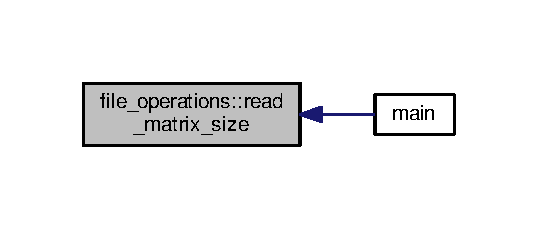
\includegraphics[width=258pt]{namespacefile__operations_aaf70668c562b4de63d013559c973421b_icgraph}
\end{center}
\end{figure}


\hypertarget{namespacefile__operations_a51aa2a1be8873c4f64256b06bf1ac578}{\index{file\-\_\-operations@{file\-\_\-operations}!read\-\_\-vector@{read\-\_\-vector}}
\index{read\-\_\-vector@{read\-\_\-vector}!file_operations@{file\-\_\-operations}}
\subsubsection[{read\-\_\-vector}]{\setlength{\rightskip}{0pt plus 5cm}template$<$class T $>$ {\bf int} file\-\_\-operations\-::read\-\_\-vector (
\begin{DoxyParamCaption}
\item[{const std\-::string \&}]{f\-\_\-name, }
\item[{size\-\_\-t}]{N, }
\item[{T $\ast$}]{vec}
\end{DoxyParamCaption}
)}}\label{namespacefile__operations_a51aa2a1be8873c4f64256b06bf1ac578}
\hypertarget{namespacefile__operations_a97599bb490f136dfc7a7acada893e864}{\index{file\-\_\-operations@{file\-\_\-operations}!write\-\_\-matrix@{write\-\_\-matrix}}
\index{write\-\_\-matrix@{write\-\_\-matrix}!file_operations@{file\-\_\-operations}}
\subsubsection[{write\-\_\-matrix}]{\setlength{\rightskip}{0pt plus 5cm}template$<$class T $>$ void file\-\_\-operations\-::write\-\_\-matrix (
\begin{DoxyParamCaption}
\item[{const std\-::string \&}]{f\-\_\-name, }
\item[{size\-\_\-t}]{Row, }
\item[{size\-\_\-t}]{Col, }
\item[{T $\ast$}]{matrix, }
\item[{unsigned {\bf int}}]{prec = {\ttfamily 17}}
\end{DoxyParamCaption}
)}}\label{namespacefile__operations_a97599bb490f136dfc7a7acada893e864}
\hypertarget{namespacefile__operations_ad47b52441906a522136b4747fb171c98}{\index{file\-\_\-operations@{file\-\_\-operations}!write\-\_\-vector@{write\-\_\-vector}}
\index{write\-\_\-vector@{write\-\_\-vector}!file_operations@{file\-\_\-operations}}
\subsubsection[{write\-\_\-vector}]{\setlength{\rightskip}{0pt plus 5cm}template$<$class T $>$ void file\-\_\-operations\-::write\-\_\-vector (
\begin{DoxyParamCaption}
\item[{const std\-::string \&}]{f\-\_\-name, }
\item[{size\-\_\-t}]{N, }
\item[{T $\ast$}]{vec, }
\item[{unsigned {\bf int}}]{prec = {\ttfamily 17}}
\end{DoxyParamCaption}
)}}\label{namespacefile__operations_ad47b52441906a522136b4747fb171c98}

\hypertarget{namespacegpu__file__operations}{\section{gpu\-\_\-file\-\_\-operations Namespace Reference}
\label{namespacegpu__file__operations}\index{gpu\-\_\-file\-\_\-operations@{gpu\-\_\-file\-\_\-operations}}
}
\subsection*{Functions}
\begin{DoxyCompactItemize}
\item 
{\footnotesize template$<$class T $>$ }\\void \hyperlink{namespacegpu__file__operations_a3e5610bf3b72d66b663fc115c6676465}{write\-\_\-vector} (const std\-::string \&f\-\_\-name, size\-\_\-t N, T $\ast$\&vec\-\_\-gpu, unsigned \hyperlink{classint}{int} prec=16)
\item 
{\footnotesize template$<$class T $>$ }\\void \hyperlink{namespacegpu__file__operations_a85070560034c559d72559d45b8b8e656}{write\-\_\-matrix} (const std\-::string \&f\-\_\-name, size\-\_\-t Row, size\-\_\-t Col, T $\ast$\&matrix\-\_\-gpu, unsigned \hyperlink{classint}{int} prec=16)
\item 
{\footnotesize template$<$class T $>$ }\\void \hyperlink{namespacegpu__file__operations_ac6be3f64ab5568f85a6bff5497f6fb77}{read\-\_\-matrix} (const std\-::string \&f\-\_\-name, size\-\_\-t Row, size\-\_\-t Col, T $\ast$\&matrix\-\_\-gpu)
\end{DoxyCompactItemize}


\subsection{Function Documentation}
\hypertarget{namespacegpu__file__operations_ac6be3f64ab5568f85a6bff5497f6fb77}{\index{gpu\-\_\-file\-\_\-operations@{gpu\-\_\-file\-\_\-operations}!read\-\_\-matrix@{read\-\_\-matrix}}
\index{read\-\_\-matrix@{read\-\_\-matrix}!gpu_file_operations@{gpu\-\_\-file\-\_\-operations}}
\subsubsection[{read\-\_\-matrix}]{\setlength{\rightskip}{0pt plus 5cm}template$<$class T $>$ void gpu\-\_\-file\-\_\-operations\-::read\-\_\-matrix (
\begin{DoxyParamCaption}
\item[{const std\-::string \&}]{f\-\_\-name, }
\item[{size\-\_\-t}]{Row, }
\item[{size\-\_\-t}]{Col, }
\item[{T $\ast$\&}]{matrix\-\_\-gpu}
\end{DoxyParamCaption}
)}}\label{namespacegpu__file__operations_ac6be3f64ab5568f85a6bff5497f6fb77}


Here is the call graph for this function\-:\nopagebreak
\begin{figure}[H]
\begin{center}
\leavevmode
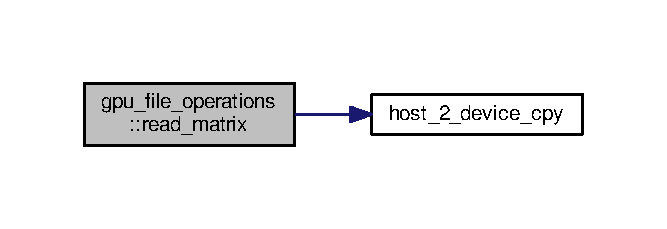
\includegraphics[width=320pt]{namespacegpu__file__operations_ac6be3f64ab5568f85a6bff5497f6fb77_cgraph}
\end{center}
\end{figure}


\hypertarget{namespacegpu__file__operations_a85070560034c559d72559d45b8b8e656}{\index{gpu\-\_\-file\-\_\-operations@{gpu\-\_\-file\-\_\-operations}!write\-\_\-matrix@{write\-\_\-matrix}}
\index{write\-\_\-matrix@{write\-\_\-matrix}!gpu_file_operations@{gpu\-\_\-file\-\_\-operations}}
\subsubsection[{write\-\_\-matrix}]{\setlength{\rightskip}{0pt plus 5cm}template$<$class T $>$ void gpu\-\_\-file\-\_\-operations\-::write\-\_\-matrix (
\begin{DoxyParamCaption}
\item[{const std\-::string \&}]{f\-\_\-name, }
\item[{size\-\_\-t}]{Row, }
\item[{size\-\_\-t}]{Col, }
\item[{T $\ast$\&}]{matrix\-\_\-gpu, }
\item[{unsigned {\bf int}}]{prec = {\ttfamily 16}}
\end{DoxyParamCaption}
)}}\label{namespacegpu__file__operations_a85070560034c559d72559d45b8b8e656}


Here is the call graph for this function\-:\nopagebreak
\begin{figure}[H]
\begin{center}
\leavevmode
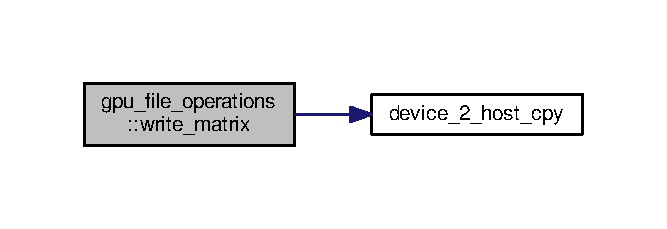
\includegraphics[width=320pt]{namespacegpu__file__operations_a85070560034c559d72559d45b8b8e656_cgraph}
\end{center}
\end{figure}


\hypertarget{namespacegpu__file__operations_a3e5610bf3b72d66b663fc115c6676465}{\index{gpu\-\_\-file\-\_\-operations@{gpu\-\_\-file\-\_\-operations}!write\-\_\-vector@{write\-\_\-vector}}
\index{write\-\_\-vector@{write\-\_\-vector}!gpu_file_operations@{gpu\-\_\-file\-\_\-operations}}
\subsubsection[{write\-\_\-vector}]{\setlength{\rightskip}{0pt plus 5cm}template$<$class T $>$ void gpu\-\_\-file\-\_\-operations\-::write\-\_\-vector (
\begin{DoxyParamCaption}
\item[{const std\-::string \&}]{f\-\_\-name, }
\item[{size\-\_\-t}]{N, }
\item[{T $\ast$\&}]{vec\-\_\-gpu, }
\item[{unsigned {\bf int}}]{prec = {\ttfamily 16}}
\end{DoxyParamCaption}
)}}\label{namespacegpu__file__operations_a3e5610bf3b72d66b663fc115c6676465}


Here is the call graph for this function\-:\nopagebreak
\begin{figure}[H]
\begin{center}
\leavevmode
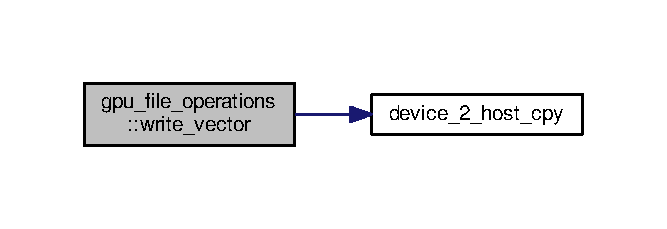
\includegraphics[width=320pt]{namespacegpu__file__operations_a3e5610bf3b72d66b663fc115c6676465_cgraph}
\end{center}
\end{figure}



\hypertarget{namespacegpu__vector__operations__type}{\section{gpu\-\_\-vector\-\_\-operations\-\_\-type Namespace Reference}
\label{namespacegpu__vector__operations__type}\index{gpu\-\_\-vector\-\_\-operations\-\_\-type@{gpu\-\_\-vector\-\_\-operations\-\_\-type}}
}
\subsection*{Classes}
\begin{DoxyCompactItemize}
\item 
struct \hyperlink{structgpu__vector__operations__type_1_1vec__ops__cuComplex__type__hlp}{vec\-\_\-ops\-\_\-cu\-Complex\-\_\-type\-\_\-hlp}
\item 
struct \hyperlink{structgpu__vector__operations__type_1_1vec__ops__cuComplex__type__hlp_3_01float_01_4}{vec\-\_\-ops\-\_\-cu\-Complex\-\_\-type\-\_\-hlp$<$ float $>$}
\item 
struct \hyperlink{structgpu__vector__operations__type_1_1vec__ops__cuComplex__type__hlp_3_01double_01_4}{vec\-\_\-ops\-\_\-cu\-Complex\-\_\-type\-\_\-hlp$<$ double $>$}
\item 
struct \hyperlink{structgpu__vector__operations__type_1_1vec__ops__cuComplex__type__hlp_3_01cuComplex_01_4}{vec\-\_\-ops\-\_\-cu\-Complex\-\_\-type\-\_\-hlp$<$ cu\-Complex $>$}
\item 
struct \hyperlink{structgpu__vector__operations__type_1_1vec__ops__cuComplex__type__hlp_3_01cuDoubleComplex_01_4}{vec\-\_\-ops\-\_\-cu\-Complex\-\_\-type\-\_\-hlp$<$ cu\-Double\-Complex $>$}
\item 
struct \hyperlink{structgpu__vector__operations__type_1_1vec__ops__cuComplex__type__hlp_3_01thrust_1_1complex_3_01float_01_4_01_4}{vec\-\_\-ops\-\_\-cu\-Complex\-\_\-type\-\_\-hlp$<$ thrust\-::complex$<$ float $>$ $>$}
\item 
struct \hyperlink{structgpu__vector__operations__type_1_1vec__ops__cuComplex__type__hlp_3_01thrust_1_1complex_3_01double_01_4_01_4}{vec\-\_\-ops\-\_\-cu\-Complex\-\_\-type\-\_\-hlp$<$ thrust\-::complex$<$ double $>$ $>$}
\end{DoxyCompactItemize}

\hypertarget{namespacenonlinear__operators}{\section{nonlinear\-\_\-operators Namespace Reference}
\label{namespacenonlinear__operators}\index{nonlinear\-\_\-operators@{nonlinear\-\_\-operators}}
}
\subsection*{Namespaces}
\begin{DoxyCompactItemize}
\item 
\hyperlink{namespacenonlinear__operators_1_1newton__method}{newton\-\_\-method}
\end{DoxyCompactItemize}
\subsection*{Classes}
\begin{DoxyCompactItemize}
\item 
class \hyperlink{classnonlinear__operators_1_1Kuramoto__Sivashinskiy__2D}{Kuramoto\-\_\-\-Sivashinskiy\-\_\-2\-D}
\item 
class \hyperlink{classnonlinear__operators_1_1linear__operator__KS__2D}{linear\-\_\-operator\-\_\-\-K\-S\-\_\-2\-D}
\item 
class \hyperlink{classnonlinear__operators_1_1preconditioner__KS__2D}{preconditioner\-\_\-\-K\-S\-\_\-2\-D}
\item 
class \hyperlink{classnonlinear__operators_1_1system__operator}{system\-\_\-operator}
\end{DoxyCompactItemize}

\hypertarget{namespacenonlinear__operators_1_1newton__method}{\section{nonlinear\-\_\-operators\-:\-:newton\-\_\-method Namespace Reference}
\label{namespacenonlinear__operators_1_1newton__method}\index{nonlinear\-\_\-operators\-::newton\-\_\-method@{nonlinear\-\_\-operators\-::newton\-\_\-method}}
}
\subsection*{Classes}
\begin{DoxyCompactItemize}
\item 
class \hyperlink{classnonlinear__operators_1_1newton__method_1_1convergence__strategy}{convergence\-\_\-strategy}
\end{DoxyCompactItemize}

\hypertarget{namespacenumerical__algos}{\section{numerical\-\_\-algos Namespace Reference}
\label{namespacenumerical__algos}\index{numerical\-\_\-algos@{numerical\-\_\-algos}}
}
\subsection*{Namespaces}
\begin{DoxyCompactItemize}
\item 
\hyperlink{namespacenumerical__algos_1_1detail}{detail}
\item 
\hyperlink{namespacenumerical__algos_1_1lin__solvers}{lin\-\_\-solvers}
\item 
\hyperlink{namespacenumerical__algos_1_1newton__method}{newton\-\_\-method}
\item 
\hyperlink{namespacenumerical__algos_1_1newton__method__extended}{newton\-\_\-method\-\_\-extended}
\item 
\hyperlink{namespacenumerical__algos_1_1sherman__morrison__linear__system}{sherman\-\_\-morrison\-\_\-linear\-\_\-system}
\end{DoxyCompactItemize}

\hypertarget{namespacenumerical__algos_1_1detail}{\section{numerical\-\_\-algos\-:\-:detail Namespace Reference}
\label{namespacenumerical__algos_1_1detail}\index{numerical\-\_\-algos\-::detail@{numerical\-\_\-algos\-::detail}}
}
\subsection*{Classes}
\begin{DoxyCompactItemize}
\item 
struct \hyperlink{structnumerical__algos_1_1detail_1_1vector__wrap}{vector\-\_\-wrap}
\item 
struct \hyperlink{structnumerical__algos_1_1detail_1_1vectors__arr__wrap__static}{vectors\-\_\-arr\-\_\-wrap\-\_\-static}
\end{DoxyCompactItemize}

\hypertarget{namespacenumerical__algos_1_1lin__solvers}{\section{numerical\-\_\-algos\-:\-:lin\-\_\-solvers Namespace Reference}
\label{namespacenumerical__algos_1_1lin__solvers}\index{numerical\-\_\-algos\-::lin\-\_\-solvers@{numerical\-\_\-algos\-::lin\-\_\-solvers}}
}
\subsection*{Namespaces}
\begin{DoxyCompactItemize}
\item 
\hyperlink{namespacenumerical__algos_1_1lin__solvers_1_1detail}{detail}
\end{DoxyCompactItemize}
\subsection*{Classes}
\begin{DoxyCompactItemize}
\item 
class \hyperlink{classnumerical__algos_1_1lin__solvers_1_1bicgstab}{bicgstab}
\item 
class \hyperlink{classnumerical__algos_1_1lin__solvers_1_1bicgstabl}{bicgstabl}
\item 
class \hyperlink{classnumerical__algos_1_1lin__solvers_1_1cgs}{cgs}
\item 
class \hyperlink{classnumerical__algos_1_1lin__solvers_1_1default__monitor}{default\-\_\-monitor}
\item 
class \hyperlink{classnumerical__algos_1_1lin__solvers_1_1iter__solver__base}{iter\-\_\-solver\-\_\-base}
\item 
class \hyperlink{classnumerical__algos_1_1lin__solvers_1_1jacobi}{jacobi}
\item 
class \hyperlink{classnumerical__algos_1_1lin__solvers_1_1lu__sgs}{lu\-\_\-sgs}
\end{DoxyCompactItemize}
\subsection*{Functions}
\begin{DoxyCompactItemize}
\item 
{\footnotesize template$<$class Vector\-Operations , class Log $>$ }\\\hyperlink{classnumerical__algos_1_1lin__solvers_1_1default__monitor}{default\-\_\-monitor}\\*
$<$ Vector\-Operations, Log $>$ $\ast$ \hyperlink{namespacenumerical__algos_1_1lin__solvers_a2a4b822ee82c023f108f2040a25b8163}{create\-\_\-monitor} (const \hyperlink{namespaceboost_1_1property__tree_aed170f35c6e34bdf310d34c11915b136}{boost\-::property\-\_\-tree\-::ptree} \&cfg, Log $\ast$log=N\-U\-L\-L, \hyperlink{classint}{int} obj\-\_\-log\-\_\-lev=0)
\item 
{\footnotesize template$<$class Linear\-Operator , class Preconditioner , class Vector\-Operations , bool Manual\-Verify\-Size, class Log $>$ }\\solver\-\_\-base$<$ Linear\-Operator, \\*
Preconditioner, \\*
Vector\-Operations, \\*
Manual\-Verify\-Size, \\*
\hyperlink{classnumerical__algos_1_1lin__solvers_1_1default__monitor}{default\-\_\-monitor}, Log $>$ $\ast$ \hyperlink{namespacenumerical__algos_1_1lin__solvers_a711dd4431c7634ce1823a19873764ffd}{create\-\_\-solver} (const \hyperlink{namespaceboost_1_1property__tree_aed170f35c6e34bdf310d34c11915b136}{boost\-::property\-\_\-tree\-::ptree} \&cfg, Log $\ast$log=N\-U\-L\-L, \hyperlink{classint}{int} obj\-\_\-log\-\_\-lev=0)
\end{DoxyCompactItemize}


\subsection{Function Documentation}
\hypertarget{namespacenumerical__algos_1_1lin__solvers_a2a4b822ee82c023f108f2040a25b8163}{\index{numerical\-\_\-algos\-::lin\-\_\-solvers@{numerical\-\_\-algos\-::lin\-\_\-solvers}!create\-\_\-monitor@{create\-\_\-monitor}}
\index{create\-\_\-monitor@{create\-\_\-monitor}!numerical_algos::lin_solvers@{numerical\-\_\-algos\-::lin\-\_\-solvers}}
\subsubsection[{create\-\_\-monitor}]{\setlength{\rightskip}{0pt plus 5cm}template$<$class Vector\-Operations , class Log $>$ {\bf default\-\_\-monitor}$<$Vector\-Operations,Log$>$$\ast$ numerical\-\_\-algos\-::lin\-\_\-solvers\-::create\-\_\-monitor (
\begin{DoxyParamCaption}
\item[{const {\bf boost\-::property\-\_\-tree\-::ptree} \&}]{cfg, }
\item[{Log $\ast$}]{log = {\ttfamily NULL}, }
\item[{{\bf int}}]{obj\-\_\-log\-\_\-lev = {\ttfamily 0}}
\end{DoxyParamCaption}
)}}\label{namespacenumerical__algos_1_1lin__solvers_a2a4b822ee82c023f108f2040a25b8163}


Here is the caller graph for this function\-:\nopagebreak
\begin{figure}[H]
\begin{center}
\leavevmode
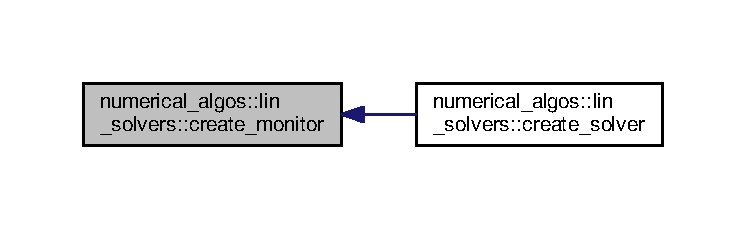
\includegraphics[width=350pt]{namespacenumerical__algos_1_1lin__solvers_a2a4b822ee82c023f108f2040a25b8163_icgraph}
\end{center}
\end{figure}


\hypertarget{namespacenumerical__algos_1_1lin__solvers_a711dd4431c7634ce1823a19873764ffd}{\index{numerical\-\_\-algos\-::lin\-\_\-solvers@{numerical\-\_\-algos\-::lin\-\_\-solvers}!create\-\_\-solver@{create\-\_\-solver}}
\index{create\-\_\-solver@{create\-\_\-solver}!numerical_algos::lin_solvers@{numerical\-\_\-algos\-::lin\-\_\-solvers}}
\subsubsection[{create\-\_\-solver}]{\setlength{\rightskip}{0pt plus 5cm}template$<$class Linear\-Operator , class Preconditioner , class Vector\-Operations , bool Manual\-Verify\-Size, class Log $>$ solver\-\_\-base$<$Linear\-Operator,Preconditioner,Vector\-Operations,Manual\-Verify\-Size,{\bf default\-\_\-monitor},Log$>$$\ast$ numerical\-\_\-algos\-::lin\-\_\-solvers\-::create\-\_\-solver (
\begin{DoxyParamCaption}
\item[{const {\bf boost\-::property\-\_\-tree\-::ptree} \&}]{cfg, }
\item[{Log $\ast$}]{log = {\ttfamily NULL}, }
\item[{{\bf int}}]{obj\-\_\-log\-\_\-lev = {\ttfamily 0}}
\end{DoxyParamCaption}
)}}\label{namespacenumerical__algos_1_1lin__solvers_a711dd4431c7634ce1823a19873764ffd}


Here is the call graph for this function\-:\nopagebreak
\begin{figure}[H]
\begin{center}
\leavevmode
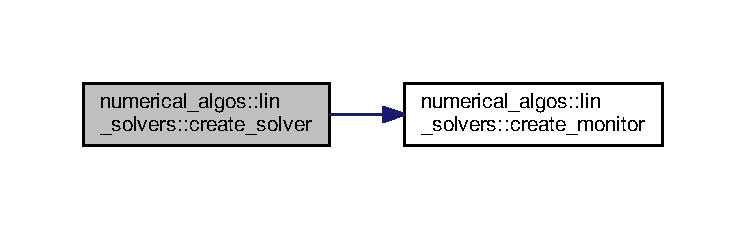
\includegraphics[width=350pt]{namespacenumerical__algos_1_1lin__solvers_a711dd4431c7634ce1823a19873764ffd_cgraph}
\end{center}
\end{figure}



\hypertarget{namespacenumerical__algos_1_1lin__solvers_1_1detail}{\section{numerical\-\_\-algos\-:\-:lin\-\_\-solvers\-:\-:detail Namespace Reference}
\label{namespacenumerical__algos_1_1lin__solvers_1_1detail}\index{numerical\-\_\-algos\-::lin\-\_\-solvers\-::detail@{numerical\-\_\-algos\-::lin\-\_\-solvers\-::detail}}
}
\subsection*{Classes}
\begin{DoxyCompactItemize}
\item 
struct \hyperlink{structnumerical__algos_1_1lin__solvers_1_1detail_1_1monitor__call__wrap}{monitor\-\_\-call\-\_\-wrap}
\end{DoxyCompactItemize}

\hypertarget{namespacenumerical__algos_1_1newton__method}{\section{numerical\-\_\-algos\-:\-:newton\-\_\-method Namespace Reference}
\label{namespacenumerical__algos_1_1newton__method}\index{numerical\-\_\-algos\-::newton\-\_\-method@{numerical\-\_\-algos\-::newton\-\_\-method}}
}
\subsection*{Classes}
\begin{DoxyCompactItemize}
\item 
class \hyperlink{classnumerical__algos_1_1newton__method_1_1newton__solver}{newton\-\_\-solver}
\end{DoxyCompactItemize}

\hypertarget{namespacenumerical__algos_1_1newton__method__extended}{\section{numerical\-\_\-algos\-:\-:newton\-\_\-method\-\_\-extended Namespace Reference}
\label{namespacenumerical__algos_1_1newton__method__extended}\index{numerical\-\_\-algos\-::newton\-\_\-method\-\_\-extended@{numerical\-\_\-algos\-::newton\-\_\-method\-\_\-extended}}
}
\subsection*{Classes}
\begin{DoxyCompactItemize}
\item 
class \hyperlink{classnumerical__algos_1_1newton__method__extended_1_1newton__solver__extended}{newton\-\_\-solver\-\_\-extended}
\end{DoxyCompactItemize}

\hypertarget{namespacenumerical__algos_1_1sherman__morrison__linear__system}{\section{numerical\-\_\-algos\-:\-:sherman\-\_\-morrison\-\_\-linear\-\_\-system Namespace Reference}
\label{namespacenumerical__algos_1_1sherman__morrison__linear__system}\index{numerical\-\_\-algos\-::sherman\-\_\-morrison\-\_\-linear\-\_\-system@{numerical\-\_\-algos\-::sherman\-\_\-morrison\-\_\-linear\-\_\-system}}
}
\subsection*{Classes}
\begin{DoxyCompactItemize}
\item 
class \hyperlink{classnumerical__algos_1_1sherman__morrison__linear__system_1_1sherman__morrison__linear__system__solve}{sherman\-\_\-morrison\-\_\-linear\-\_\-system\-\_\-solve}
\end{DoxyCompactItemize}

\hypertarget{namespacetest__class}{\section{test\-\_\-class Namespace Reference}
\label{namespacetest__class}\index{test\-\_\-class@{test\-\_\-class}}
}
\subsection*{Classes}
\begin{DoxyCompactItemize}
\item 
class \hyperlink{classtest__class_1_1class__file}{class\-\_\-file}
\end{DoxyCompactItemize}

\hypertarget{namespaceutils}{\section{utils Namespace Reference}
\label{namespaceutils}\index{utils@{utils}}
}
\subsection*{Classes}
\begin{DoxyCompactItemize}
\item 
struct \hyperlink{structutils_1_1cuda__timer__event}{cuda\-\_\-timer\-\_\-event}
\item 
class \hyperlink{classutils_1_1log}{log}
\item 
class \hyperlink{classutils_1_1log__std}{log\-\_\-std}
\item 
class \hyperlink{classutils_1_1log__mpi}{log\-\_\-mpi}
\item 
class \hyperlink{classutils_1_1logged__obj__base}{logged\-\_\-obj\-\_\-base}
\item 
struct \hyperlink{structutils_1_1mpi__timer__event}{mpi\-\_\-timer\-\_\-event}
\item 
struct \hyperlink{structutils_1_1system__timer__event}{system\-\_\-timer\-\_\-event}
\item 
struct \hyperlink{structutils_1_1timer__event}{timer\-\_\-event}
\item 
struct \hyperlink{structutils_1_1vals__table__1d}{vals\-\_\-table\-\_\-1d}
\item 
struct \hyperlink{structutils_1_1vals__table__2d}{vals\-\_\-table\-\_\-2d}
\item 
struct \hyperlink{structutils_1_1vals__table__3d}{vals\-\_\-table\-\_\-3d}
\item 
struct \hyperlink{structutils_1_1vals__table__4d}{vals\-\_\-table\-\_\-4d}
\end{DoxyCompactItemize}
\subsection*{Functions}
\begin{DoxyCompactItemize}
\item 
bool \hyperlink{namespaceutils_acd1c75c1806c282769faabc87cfa93dc}{init\-\_\-cuda} (\hyperlink{classint}{int} user\-\_\-prefered\-\_\-i=-\/1)
\end{DoxyCompactItemize}


\subsection{Function Documentation}
\hypertarget{namespaceutils_acd1c75c1806c282769faabc87cfa93dc}{\index{utils@{utils}!init\-\_\-cuda@{init\-\_\-cuda}}
\index{init\-\_\-cuda@{init\-\_\-cuda}!utils@{utils}}
\subsubsection[{init\-\_\-cuda}]{\setlength{\rightskip}{0pt plus 5cm}bool utils\-::init\-\_\-cuda (
\begin{DoxyParamCaption}
\item[{{\bf int}}]{user\-\_\-prefered\-\_\-i = {\ttfamily -\/1}}
\end{DoxyParamCaption}
)\hspace{0.3cm}{\ttfamily [inline]}}}\label{namespaceutils_acd1c75c1806c282769faabc87cfa93dc}

\chapter{Class Documentation}
\hypertarget{classcontinuation_1_1advance__solution}{\section{continuation\-:\-:advance\-\_\-solution$<$ Vector\-Operations, Loggin, Newton\-Method, Nonlinear\-Operator, System\-Operator, Predictoror $>$ Class Template Reference}
\label{classcontinuation_1_1advance__solution}\index{continuation\-::advance\-\_\-solution$<$ Vector\-Operations, Loggin, Newton\-Method, Nonlinear\-Operator, System\-Operator, Predictoror $>$@{continuation\-::advance\-\_\-solution$<$ Vector\-Operations, Loggin, Newton\-Method, Nonlinear\-Operator, System\-Operator, Predictoror $>$}}
}


{\ttfamily \#include $<$advance\-\_\-solution.\-h$>$}



Collaboration diagram for continuation\-:\-:advance\-\_\-solution$<$ Vector\-Operations, Loggin, Newton\-Method, Nonlinear\-Operator, System\-Operator, Predictoror $>$\-:
\nopagebreak
\begin{figure}[H]
\begin{center}
\leavevmode
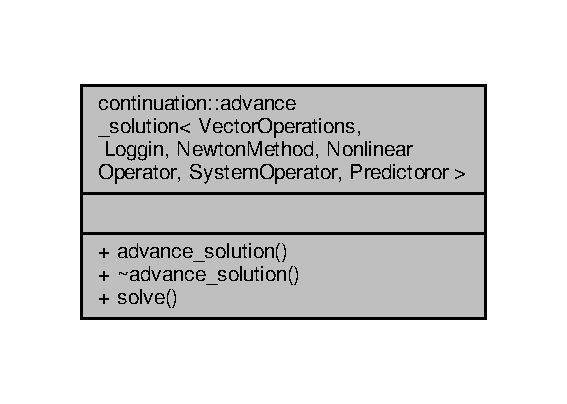
\includegraphics[width=272pt]{classcontinuation_1_1advance__solution__coll__graph}
\end{center}
\end{figure}
\subsection*{Public Types}
\begin{DoxyCompactItemize}
\item 
typedef \\*
Vector\-Operations\-::scalar\-\_\-type \hyperlink{classcontinuation_1_1advance__solution_a525792bcc16846c5ba10f15400d53fed}{T}
\item 
typedef \\*
Vector\-Operations\-::vector\-\_\-type \hyperlink{classcontinuation_1_1advance__solution_a2c54f76f6415c6d28af4c97f7d6fe605}{T\-\_\-vec}
\end{DoxyCompactItemize}
\subsection*{Public Member Functions}
\begin{DoxyCompactItemize}
\item 
\hyperlink{classcontinuation_1_1advance__solution_a431534d391d29365c19fd7e67bd23459}{advance\-\_\-solution} (Vector\-Operations $\ast$vec\-\_\-ops\-\_\-, Loggin $\ast$log\-\_\-, System\-Operator $\ast$sys\-\_\-op\-\_\-, Newton\-Method $\ast$newton\-\_\-, Predictoror $\ast$predictor\-\_\-)
\item 
\hyperlink{classcontinuation_1_1advance__solution_a81ccd4bfac143b8d6c6a648ba8917f96}{$\sim$advance\-\_\-solution} ()
\item 
bool \hyperlink{classcontinuation_1_1advance__solution_aad61441232f6e12769db1c16214d61cf}{solve} (Nonlinear\-Operator $\ast$nonlin\-\_\-op, const \hyperlink{classcontinuation_1_1advance__solution_a2c54f76f6415c6d28af4c97f7d6fe605}{T\-\_\-vec} \&x0, const \hyperlink{classcontinuation_1_1advance__solution_a525792bcc16846c5ba10f15400d53fed}{T} \&lambda0, const \hyperlink{classcontinuation_1_1advance__solution_a2c54f76f6415c6d28af4c97f7d6fe605}{T\-\_\-vec} \&x0\-\_\-s, const \hyperlink{classcontinuation_1_1advance__solution_a525792bcc16846c5ba10f15400d53fed}{T} \&lambda0\-\_\-s, \hyperlink{classcontinuation_1_1advance__solution_a2c54f76f6415c6d28af4c97f7d6fe605}{T\-\_\-vec} \&x1, \hyperlink{classcontinuation_1_1advance__solution_a525792bcc16846c5ba10f15400d53fed}{T} \&lambda1, \hyperlink{classcontinuation_1_1advance__solution_a2c54f76f6415c6d28af4c97f7d6fe605}{T\-\_\-vec} \&x1\-\_\-s, \hyperlink{classcontinuation_1_1advance__solution_a525792bcc16846c5ba10f15400d53fed}{T} \&lambda1\-\_\-s)
\end{DoxyCompactItemize}


\subsection{Member Typedef Documentation}
\hypertarget{classcontinuation_1_1advance__solution_a525792bcc16846c5ba10f15400d53fed}{\index{continuation\-::advance\-\_\-solution@{continuation\-::advance\-\_\-solution}!T@{T}}
\index{T@{T}!continuation::advance_solution@{continuation\-::advance\-\_\-solution}}
\subsubsection[{T}]{\setlength{\rightskip}{0pt plus 5cm}template$<$class Vector\-Operations , class Loggin , class Newton\-Method , class Nonlinear\-Operator , class System\-Operator , class Predictoror $>$ typedef Vector\-Operations\-::scalar\-\_\-type {\bf continuation\-::advance\-\_\-solution}$<$ Vector\-Operations, Loggin, Newton\-Method, Nonlinear\-Operator, System\-Operator, Predictoror $>$\-::{\bf T}}}\label{classcontinuation_1_1advance__solution_a525792bcc16846c5ba10f15400d53fed}
\hypertarget{classcontinuation_1_1advance__solution_a2c54f76f6415c6d28af4c97f7d6fe605}{\index{continuation\-::advance\-\_\-solution@{continuation\-::advance\-\_\-solution}!T\-\_\-vec@{T\-\_\-vec}}
\index{T\-\_\-vec@{T\-\_\-vec}!continuation::advance_solution@{continuation\-::advance\-\_\-solution}}
\subsubsection[{T\-\_\-vec}]{\setlength{\rightskip}{0pt plus 5cm}template$<$class Vector\-Operations , class Loggin , class Newton\-Method , class Nonlinear\-Operator , class System\-Operator , class Predictoror $>$ typedef Vector\-Operations\-::vector\-\_\-type {\bf continuation\-::advance\-\_\-solution}$<$ Vector\-Operations, Loggin, Newton\-Method, Nonlinear\-Operator, System\-Operator, Predictoror $>$\-::{\bf T\-\_\-vec}}}\label{classcontinuation_1_1advance__solution_a2c54f76f6415c6d28af4c97f7d6fe605}


\subsection{Constructor \& Destructor Documentation}
\hypertarget{classcontinuation_1_1advance__solution_a431534d391d29365c19fd7e67bd23459}{\index{continuation\-::advance\-\_\-solution@{continuation\-::advance\-\_\-solution}!advance\-\_\-solution@{advance\-\_\-solution}}
\index{advance\-\_\-solution@{advance\-\_\-solution}!continuation::advance_solution@{continuation\-::advance\-\_\-solution}}
\subsubsection[{advance\-\_\-solution}]{\setlength{\rightskip}{0pt plus 5cm}template$<$class Vector\-Operations , class Loggin , class Newton\-Method , class Nonlinear\-Operator , class System\-Operator , class Predictoror $>$ {\bf continuation\-::advance\-\_\-solution}$<$ Vector\-Operations, Loggin, Newton\-Method, Nonlinear\-Operator, System\-Operator, Predictoror $>$\-::{\bf advance\-\_\-solution} (
\begin{DoxyParamCaption}
\item[{Vector\-Operations $\ast$}]{vec\-\_\-ops\-\_\-, }
\item[{Loggin $\ast$}]{log\-\_\-, }
\item[{System\-Operator $\ast$}]{sys\-\_\-op\-\_\-, }
\item[{Newton\-Method $\ast$}]{newton\-\_\-, }
\item[{Predictoror $\ast$}]{predictor\-\_\-}
\end{DoxyParamCaption}
)\hspace{0.3cm}{\ttfamily [inline]}}}\label{classcontinuation_1_1advance__solution_a431534d391d29365c19fd7e67bd23459}
\hypertarget{classcontinuation_1_1advance__solution_a81ccd4bfac143b8d6c6a648ba8917f96}{\index{continuation\-::advance\-\_\-solution@{continuation\-::advance\-\_\-solution}!$\sim$advance\-\_\-solution@{$\sim$advance\-\_\-solution}}
\index{$\sim$advance\-\_\-solution@{$\sim$advance\-\_\-solution}!continuation::advance_solution@{continuation\-::advance\-\_\-solution}}
\subsubsection[{$\sim$advance\-\_\-solution}]{\setlength{\rightskip}{0pt plus 5cm}template$<$class Vector\-Operations , class Loggin , class Newton\-Method , class Nonlinear\-Operator , class System\-Operator , class Predictoror $>$ {\bf continuation\-::advance\-\_\-solution}$<$ Vector\-Operations, Loggin, Newton\-Method, Nonlinear\-Operator, System\-Operator, Predictoror $>$\-::$\sim${\bf advance\-\_\-solution} (
\begin{DoxyParamCaption}
{}
\end{DoxyParamCaption}
)\hspace{0.3cm}{\ttfamily [inline]}}}\label{classcontinuation_1_1advance__solution_a81ccd4bfac143b8d6c6a648ba8917f96}


\subsection{Member Function Documentation}
\hypertarget{classcontinuation_1_1advance__solution_aad61441232f6e12769db1c16214d61cf}{\index{continuation\-::advance\-\_\-solution@{continuation\-::advance\-\_\-solution}!solve@{solve}}
\index{solve@{solve}!continuation::advance_solution@{continuation\-::advance\-\_\-solution}}
\subsubsection[{solve}]{\setlength{\rightskip}{0pt plus 5cm}template$<$class Vector\-Operations , class Loggin , class Newton\-Method , class Nonlinear\-Operator , class System\-Operator , class Predictoror $>$ bool {\bf continuation\-::advance\-\_\-solution}$<$ Vector\-Operations, Loggin, Newton\-Method, Nonlinear\-Operator, System\-Operator, Predictoror $>$\-::solve (
\begin{DoxyParamCaption}
\item[{Nonlinear\-Operator $\ast$}]{nonlin\-\_\-op, }
\item[{const {\bf T\-\_\-vec} \&}]{x0, }
\item[{const {\bf T} \&}]{lambda0, }
\item[{const {\bf T\-\_\-vec} \&}]{x0\-\_\-s, }
\item[{const {\bf T} \&}]{lambda0\-\_\-s, }
\item[{{\bf T\-\_\-vec} \&}]{x1, }
\item[{{\bf T} \&}]{lambda1, }
\item[{{\bf T\-\_\-vec} \&}]{x1\-\_\-s, }
\item[{{\bf T} \&}]{lambda1\-\_\-s}
\end{DoxyParamCaption}
)\hspace{0.3cm}{\ttfamily [inline]}}}\label{classcontinuation_1_1advance__solution_aad61441232f6e12769db1c16214d61cf}


Here is the caller graph for this function\-:
\nopagebreak
\begin{figure}[H]
\begin{center}
\leavevmode
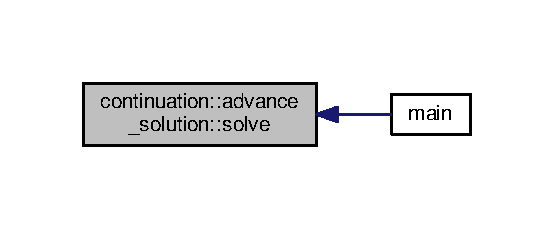
\includegraphics[width=266pt]{classcontinuation_1_1advance__solution_aad61441232f6e12769db1c16214d61cf_icgraph}
\end{center}
\end{figure}




The documentation for this class was generated from the following file\-:\begin{DoxyCompactItemize}
\item 
source/continuation/\hyperlink{advance__solution_8h}{advance\-\_\-solution.\-h}\end{DoxyCompactItemize}

\hypertarget{classboost_1_1property__tree_1_1basic__ptree}{\section{boost\-:\-:property\-\_\-tree\-:\-:basic\-\_\-ptree$<$ Key, Data, Key\-Compare $>$ Class Template Reference}
\label{classboost_1_1property__tree_1_1basic__ptree}\index{boost\-::property\-\_\-tree\-::basic\-\_\-ptree$<$ Key, Data, Key\-Compare $>$@{boost\-::property\-\_\-tree\-::basic\-\_\-ptree$<$ Key, Data, Key\-Compare $>$}}
}


{\ttfamily \#include $<$boost\-\_\-property\-\_\-tree\-\_\-fwd.\-h$>$}



Collaboration diagram for boost\-:\-:property\-\_\-tree\-:\-:basic\-\_\-ptree$<$ Key, Data, Key\-Compare $>$\-:\nopagebreak
\begin{figure}[H]
\begin{center}
\leavevmode
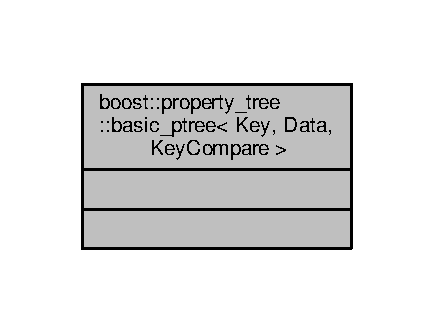
\includegraphics[width=208pt]{classboost_1_1property__tree_1_1basic__ptree__coll__graph}
\end{center}
\end{figure}


The documentation for this class was generated from the following file\-:\begin{DoxyCompactItemize}
\item 
source/utils/\hyperlink{boost__property__tree__fwd_8h}{boost\-\_\-property\-\_\-tree\-\_\-fwd.\-h}\end{DoxyCompactItemize}

\hypertarget{classnumerical__algos_1_1lin__solvers_1_1bicgstab}{\section{numerical\-\_\-algos\-:\-:lin\-\_\-solvers\-:\-:bicgstab$<$ Linear\-Operator, Preconditioner, Vector\-Operations, Monitor, Log $>$ Class Template Reference}
\label{classnumerical__algos_1_1lin__solvers_1_1bicgstab}\index{numerical\-\_\-algos\-::lin\-\_\-solvers\-::bicgstab$<$ Linear\-Operator, Preconditioner, Vector\-Operations, Monitor, Log $>$@{numerical\-\_\-algos\-::lin\-\_\-solvers\-::bicgstab$<$ Linear\-Operator, Preconditioner, Vector\-Operations, Monitor, Log $>$}}
}


{\ttfamily \#include $<$bicgstab.\-h$>$}



Inheritance diagram for numerical\-\_\-algos\-:\-:lin\-\_\-solvers\-:\-:bicgstab$<$ Linear\-Operator, Preconditioner, Vector\-Operations, Monitor, Log $>$\-:
\nopagebreak
\begin{figure}[H]
\begin{center}
\leavevmode
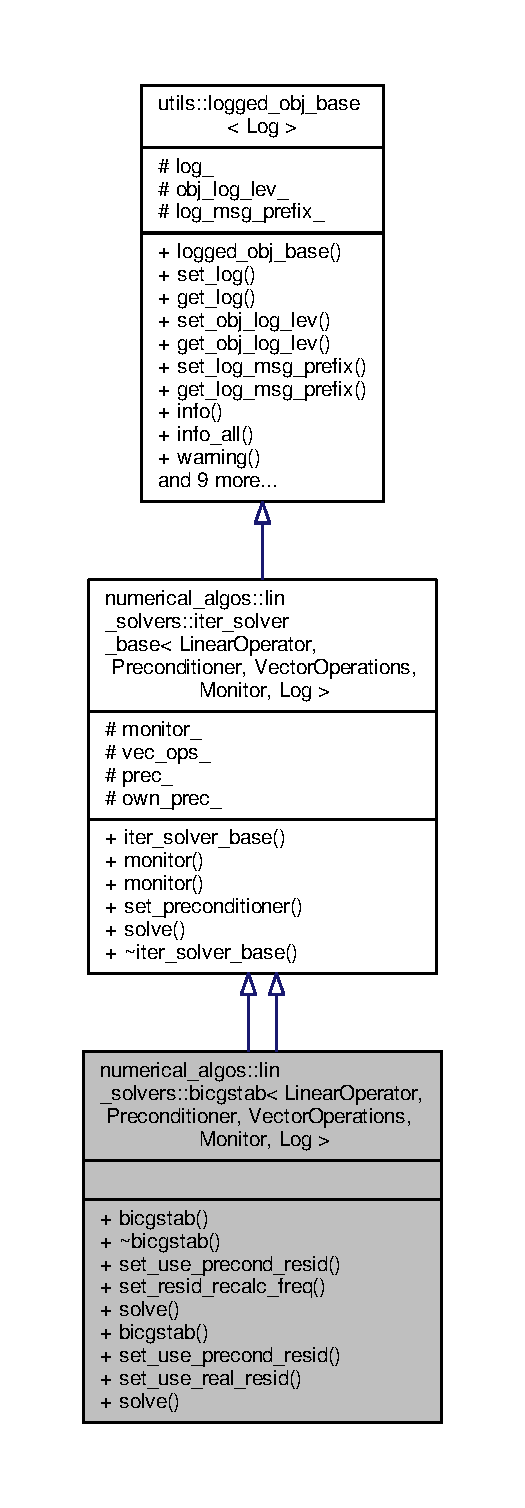
\includegraphics[height=550pt]{classnumerical__algos_1_1lin__solvers_1_1bicgstab__inherit__graph}
\end{center}
\end{figure}


Collaboration diagram for numerical\-\_\-algos\-:\-:lin\-\_\-solvers\-:\-:bicgstab$<$ Linear\-Operator, Preconditioner, Vector\-Operations, Monitor, Log $>$\-:
\nopagebreak
\begin{figure}[H]
\begin{center}
\leavevmode
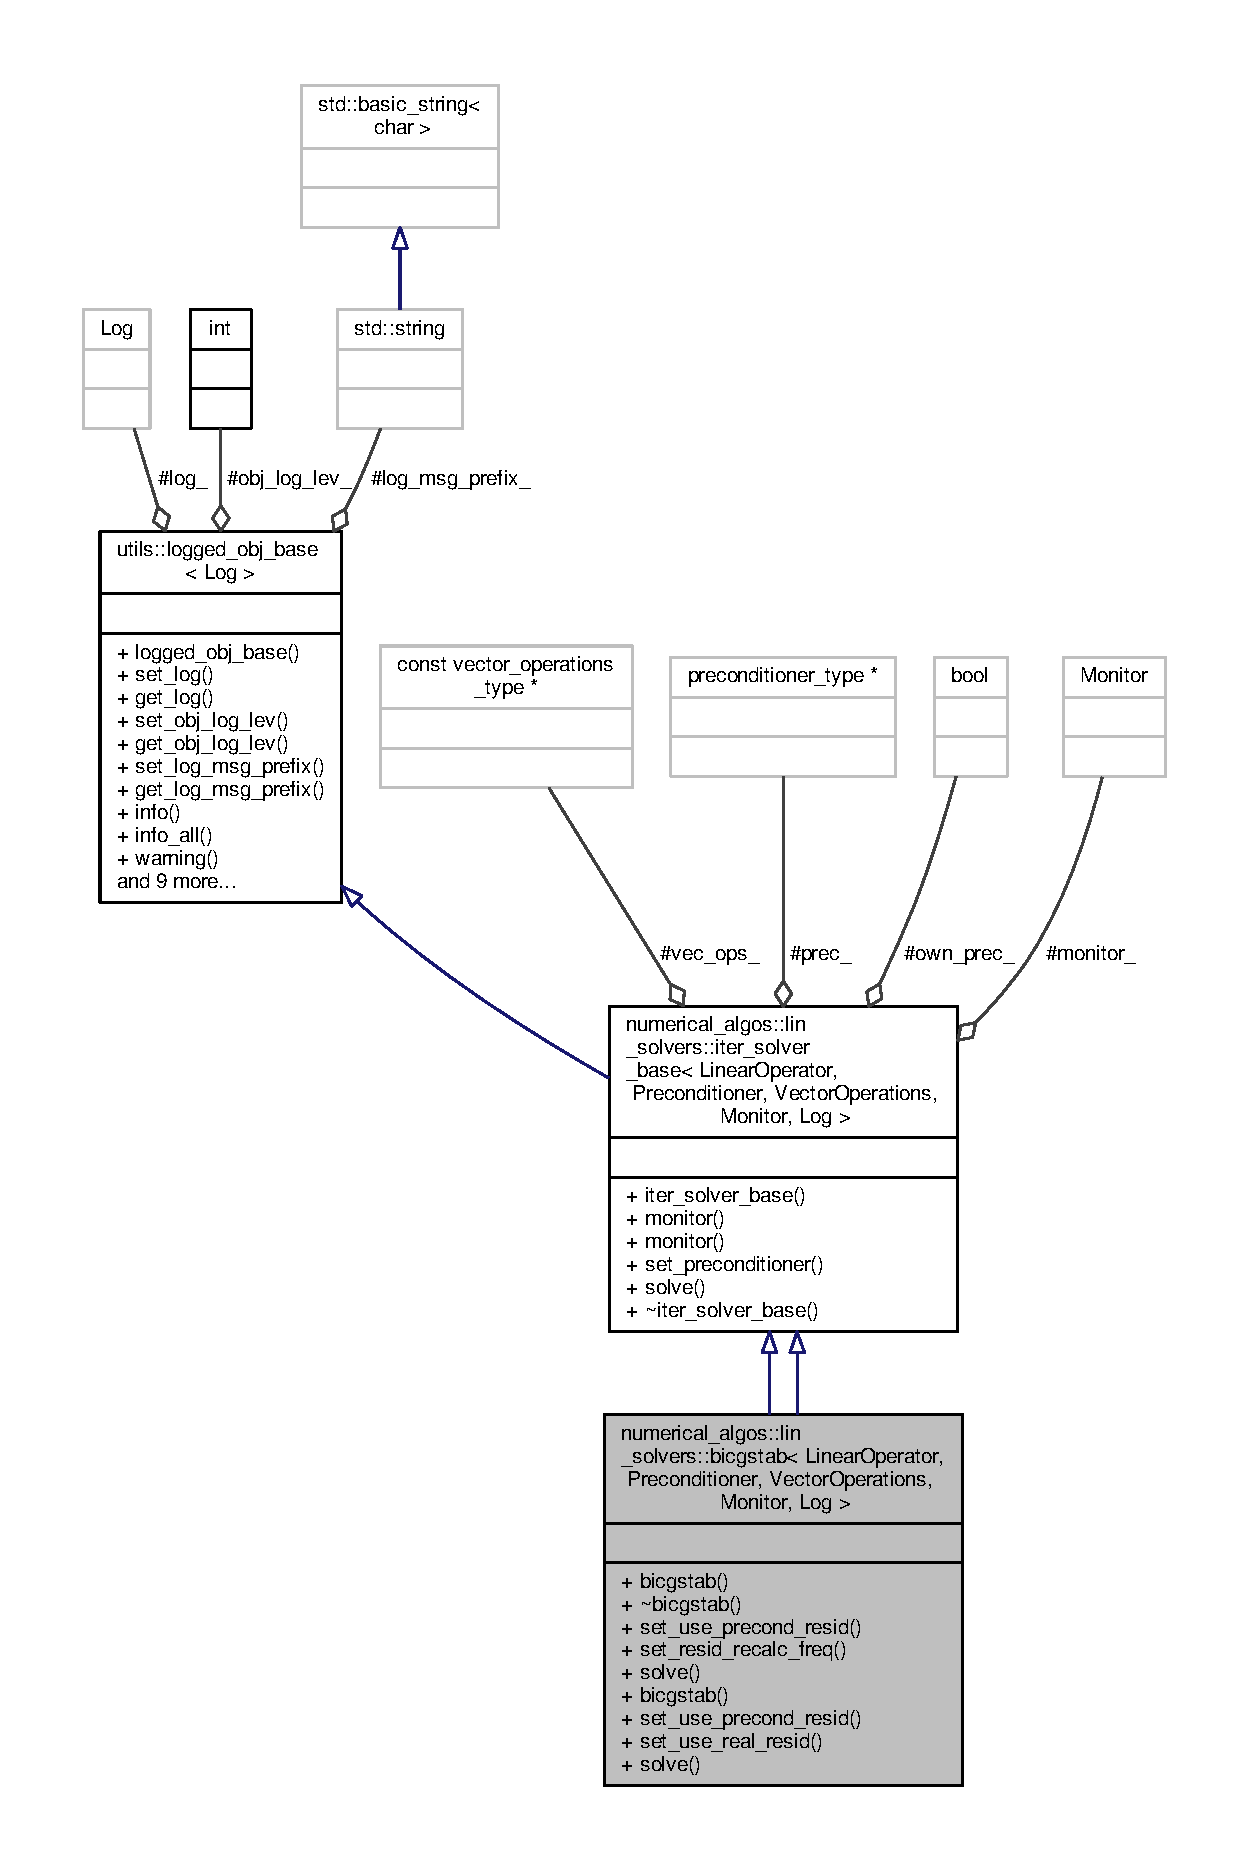
\includegraphics[width=350pt]{classnumerical__algos_1_1lin__solvers_1_1bicgstab__coll__graph}
\end{center}
\end{figure}
\subsection*{Public Types}
\begin{DoxyCompactItemize}
\item 
typedef \\*
Vector\-Operations\-::scalar\-\_\-type \hyperlink{classnumerical__algos_1_1lin__solvers_1_1bicgstab_a051c0387d2b7f9c86883a0e612291876}{scalar\-\_\-type}
\item 
typedef \\*
Vector\-Operations\-::vector\-\_\-type \hyperlink{classnumerical__algos_1_1lin__solvers_1_1bicgstab_a3525de8fe1598864ceac98c83bd0d477}{vector\-\_\-type}
\item 
typedef Linear\-Operator \hyperlink{classnumerical__algos_1_1lin__solvers_1_1bicgstab_a77f7bc99b7f22986f73ce7d2b4ebd669}{linear\-\_\-operator\-\_\-type}
\item 
typedef Preconditioner \hyperlink{classnumerical__algos_1_1lin__solvers_1_1bicgstab_a70df69cdff2a33dea49471b873ca91af}{preconditioner\-\_\-type}
\item 
typedef Vector\-Operations \hyperlink{classnumerical__algos_1_1lin__solvers_1_1bicgstab_a6ff5c085063b744de8b72fd42bd45f33}{vector\-\_\-operations\-\_\-type}
\item 
typedef Monitor \hyperlink{classnumerical__algos_1_1lin__solvers_1_1bicgstab_a5837507942b23f73613452c79032b795}{monitor\-\_\-type}
\item 
typedef Log \hyperlink{classnumerical__algos_1_1lin__solvers_1_1bicgstab_a89196ef8d314663bd606395a4c8a6cc1}{log\-\_\-type}
\item 
typedef \\*
Vector\-Operations\-::scalar\-\_\-type \hyperlink{classnumerical__algos_1_1lin__solvers_1_1bicgstab_a051c0387d2b7f9c86883a0e612291876}{scalar\-\_\-type}
\item 
typedef \\*
Vector\-Operations\-::vector\-\_\-type \hyperlink{classnumerical__algos_1_1lin__solvers_1_1bicgstab_a3525de8fe1598864ceac98c83bd0d477}{vector\-\_\-type}
\item 
typedef Linear\-Operator \hyperlink{classnumerical__algos_1_1lin__solvers_1_1bicgstab_a77f7bc99b7f22986f73ce7d2b4ebd669}{linear\-\_\-operator\-\_\-type}
\item 
typedef Preconditioner \hyperlink{classnumerical__algos_1_1lin__solvers_1_1bicgstab_a70df69cdff2a33dea49471b873ca91af}{preconditioner\-\_\-type}
\item 
typedef Vector\-Operations \hyperlink{classnumerical__algos_1_1lin__solvers_1_1bicgstab_a6ff5c085063b744de8b72fd42bd45f33}{vector\-\_\-operations\-\_\-type}
\item 
typedef Monitor \hyperlink{classnumerical__algos_1_1lin__solvers_1_1bicgstab_a5837507942b23f73613452c79032b795}{monitor\-\_\-type}
\item 
typedef Log \hyperlink{classnumerical__algos_1_1lin__solvers_1_1bicgstab_a89196ef8d314663bd606395a4c8a6cc1}{log\-\_\-type}
\end{DoxyCompactItemize}
\subsection*{Public Member Functions}
\begin{DoxyCompactItemize}
\item 
\hyperlink{classnumerical__algos_1_1lin__solvers_1_1bicgstab_a2ef7808628f564b8cdc9aed0f108ebda}{bicgstab} (const \hyperlink{classnumerical__algos_1_1lin__solvers_1_1bicgstab_a6ff5c085063b744de8b72fd42bd45f33}{vector\-\_\-operations\-\_\-type} $\ast$vec\-\_\-ops, Log $\ast$log=N\-U\-L\-L, \hyperlink{classint}{int} obj\-\_\-log\-\_\-lev=0)
\item 
\hyperlink{classnumerical__algos_1_1lin__solvers_1_1bicgstab_ae84e9e1ede472200f7f2ca5eacbb4389}{$\sim$bicgstab} ()
\item 
void \hyperlink{classnumerical__algos_1_1lin__solvers_1_1bicgstab_a61ef325066d9edb6529fb1fca673d6c1}{set\-\_\-use\-\_\-precond\-\_\-resid} (bool use\-\_\-precond\-\_\-resid)
\item 
void \hyperlink{classnumerical__algos_1_1lin__solvers_1_1bicgstab_a9f90b0901edd43e3c67d900688e436d3}{set\-\_\-resid\-\_\-recalc\-\_\-freq} (\hyperlink{classint}{int} resid\-\_\-recalc\-\_\-freq)
\item 
virtual bool \hyperlink{classnumerical__algos_1_1lin__solvers_1_1bicgstab_ac3df95058825e4a8a1ed6bf838f10669}{solve} (const \hyperlink{classnumerical__algos_1_1lin__solvers_1_1bicgstab_a77f7bc99b7f22986f73ce7d2b4ebd669}{linear\-\_\-operator\-\_\-type} \&A, const \hyperlink{classnumerical__algos_1_1lin__solvers_1_1bicgstab_a3525de8fe1598864ceac98c83bd0d477}{vector\-\_\-type} \&b, \hyperlink{classnumerical__algos_1_1lin__solvers_1_1bicgstab_a3525de8fe1598864ceac98c83bd0d477}{vector\-\_\-type} \&x) const 
\item 
\hyperlink{classnumerical__algos_1_1lin__solvers_1_1bicgstab_a2ef7808628f564b8cdc9aed0f108ebda}{bicgstab} (const \hyperlink{classnumerical__algos_1_1lin__solvers_1_1bicgstab_a6ff5c085063b744de8b72fd42bd45f33}{vector\-\_\-operations\-\_\-type} $\ast$vec\-\_\-ops, Log $\ast$log=N\-U\-L\-L, \hyperlink{classint}{int} obj\-\_\-log\-\_\-lev=0)
\item 
void \hyperlink{classnumerical__algos_1_1lin__solvers_1_1bicgstab_a61ef325066d9edb6529fb1fca673d6c1}{set\-\_\-use\-\_\-precond\-\_\-resid} (bool use\-\_\-precond\-\_\-resid)
\item 
void \hyperlink{classnumerical__algos_1_1lin__solvers_1_1bicgstab_ae69b7e9da24cba334a330781d0f00c98}{set\-\_\-use\-\_\-real\-\_\-resid} (bool use\-\_\-real\-\_\-resid)
\item 
virtual bool \hyperlink{classnumerical__algos_1_1lin__solvers_1_1bicgstab_ac3df95058825e4a8a1ed6bf838f10669}{solve} (const \hyperlink{classnumerical__algos_1_1lin__solvers_1_1bicgstab_a77f7bc99b7f22986f73ce7d2b4ebd669}{linear\-\_\-operator\-\_\-type} \&A, const \hyperlink{classnumerical__algos_1_1lin__solvers_1_1bicgstab_a3525de8fe1598864ceac98c83bd0d477}{vector\-\_\-type} \&b, \hyperlink{classnumerical__algos_1_1lin__solvers_1_1bicgstab_a3525de8fe1598864ceac98c83bd0d477}{vector\-\_\-type} \&x) const 
\end{DoxyCompactItemize}
\subsection*{Additional Inherited Members}


\subsection{Member Typedef Documentation}
\hypertarget{classnumerical__algos_1_1lin__solvers_1_1bicgstab_a77f7bc99b7f22986f73ce7d2b4ebd669}{\index{numerical\-\_\-algos\-::lin\-\_\-solvers\-::bicgstab@{numerical\-\_\-algos\-::lin\-\_\-solvers\-::bicgstab}!linear\-\_\-operator\-\_\-type@{linear\-\_\-operator\-\_\-type}}
\index{linear\-\_\-operator\-\_\-type@{linear\-\_\-operator\-\_\-type}!numerical_algos::lin_solvers::bicgstab@{numerical\-\_\-algos\-::lin\-\_\-solvers\-::bicgstab}}
\subsubsection[{linear\-\_\-operator\-\_\-type}]{\setlength{\rightskip}{0pt plus 5cm}template$<$class Linear\-Operator , class Preconditioner , class Vector\-Operations , class Monitor , class Log $>$ typedef Linear\-Operator {\bf numerical\-\_\-algos\-::lin\-\_\-solvers\-::bicgstab}$<$ Linear\-Operator, Preconditioner, Vector\-Operations, Monitor, Log $>$\-::{\bf linear\-\_\-operator\-\_\-type}}}\label{classnumerical__algos_1_1lin__solvers_1_1bicgstab_a77f7bc99b7f22986f73ce7d2b4ebd669}
\hypertarget{classnumerical__algos_1_1lin__solvers_1_1bicgstab_a77f7bc99b7f22986f73ce7d2b4ebd669}{\index{numerical\-\_\-algos\-::lin\-\_\-solvers\-::bicgstab@{numerical\-\_\-algos\-::lin\-\_\-solvers\-::bicgstab}!linear\-\_\-operator\-\_\-type@{linear\-\_\-operator\-\_\-type}}
\index{linear\-\_\-operator\-\_\-type@{linear\-\_\-operator\-\_\-type}!numerical_algos::lin_solvers::bicgstab@{numerical\-\_\-algos\-::lin\-\_\-solvers\-::bicgstab}}
\subsubsection[{linear\-\_\-operator\-\_\-type}]{\setlength{\rightskip}{0pt plus 5cm}template$<$class Linear\-Operator , class Preconditioner , class Vector\-Operations , class Monitor , class Log $>$ typedef Linear\-Operator {\bf numerical\-\_\-algos\-::lin\-\_\-solvers\-::bicgstab}$<$ Linear\-Operator, Preconditioner, Vector\-Operations, Monitor, Log $>$\-::{\bf linear\-\_\-operator\-\_\-type}}}\label{classnumerical__algos_1_1lin__solvers_1_1bicgstab_a77f7bc99b7f22986f73ce7d2b4ebd669}
\hypertarget{classnumerical__algos_1_1lin__solvers_1_1bicgstab_a89196ef8d314663bd606395a4c8a6cc1}{\index{numerical\-\_\-algos\-::lin\-\_\-solvers\-::bicgstab@{numerical\-\_\-algos\-::lin\-\_\-solvers\-::bicgstab}!log\-\_\-type@{log\-\_\-type}}
\index{log\-\_\-type@{log\-\_\-type}!numerical_algos::lin_solvers::bicgstab@{numerical\-\_\-algos\-::lin\-\_\-solvers\-::bicgstab}}
\subsubsection[{log\-\_\-type}]{\setlength{\rightskip}{0pt plus 5cm}template$<$class Linear\-Operator , class Preconditioner , class Vector\-Operations , class Monitor , class Log $>$ typedef Log {\bf numerical\-\_\-algos\-::lin\-\_\-solvers\-::bicgstab}$<$ Linear\-Operator, Preconditioner, Vector\-Operations, Monitor, Log $>$\-::{\bf log\-\_\-type}}}\label{classnumerical__algos_1_1lin__solvers_1_1bicgstab_a89196ef8d314663bd606395a4c8a6cc1}
\hypertarget{classnumerical__algos_1_1lin__solvers_1_1bicgstab_a89196ef8d314663bd606395a4c8a6cc1}{\index{numerical\-\_\-algos\-::lin\-\_\-solvers\-::bicgstab@{numerical\-\_\-algos\-::lin\-\_\-solvers\-::bicgstab}!log\-\_\-type@{log\-\_\-type}}
\index{log\-\_\-type@{log\-\_\-type}!numerical_algos::lin_solvers::bicgstab@{numerical\-\_\-algos\-::lin\-\_\-solvers\-::bicgstab}}
\subsubsection[{log\-\_\-type}]{\setlength{\rightskip}{0pt plus 5cm}template$<$class Linear\-Operator , class Preconditioner , class Vector\-Operations , class Monitor , class Log $>$ typedef Log {\bf numerical\-\_\-algos\-::lin\-\_\-solvers\-::bicgstab}$<$ Linear\-Operator, Preconditioner, Vector\-Operations, Monitor, Log $>$\-::{\bf log\-\_\-type}}}\label{classnumerical__algos_1_1lin__solvers_1_1bicgstab_a89196ef8d314663bd606395a4c8a6cc1}
\hypertarget{classnumerical__algos_1_1lin__solvers_1_1bicgstab_a5837507942b23f73613452c79032b795}{\index{numerical\-\_\-algos\-::lin\-\_\-solvers\-::bicgstab@{numerical\-\_\-algos\-::lin\-\_\-solvers\-::bicgstab}!monitor\-\_\-type@{monitor\-\_\-type}}
\index{monitor\-\_\-type@{monitor\-\_\-type}!numerical_algos::lin_solvers::bicgstab@{numerical\-\_\-algos\-::lin\-\_\-solvers\-::bicgstab}}
\subsubsection[{monitor\-\_\-type}]{\setlength{\rightskip}{0pt plus 5cm}template$<$class Linear\-Operator , class Preconditioner , class Vector\-Operations , class Monitor , class Log $>$ typedef Monitor {\bf numerical\-\_\-algos\-::lin\-\_\-solvers\-::bicgstab}$<$ Linear\-Operator, Preconditioner, Vector\-Operations, Monitor, Log $>$\-::{\bf monitor\-\_\-type}}}\label{classnumerical__algos_1_1lin__solvers_1_1bicgstab_a5837507942b23f73613452c79032b795}
\hypertarget{classnumerical__algos_1_1lin__solvers_1_1bicgstab_a5837507942b23f73613452c79032b795}{\index{numerical\-\_\-algos\-::lin\-\_\-solvers\-::bicgstab@{numerical\-\_\-algos\-::lin\-\_\-solvers\-::bicgstab}!monitor\-\_\-type@{monitor\-\_\-type}}
\index{monitor\-\_\-type@{monitor\-\_\-type}!numerical_algos::lin_solvers::bicgstab@{numerical\-\_\-algos\-::lin\-\_\-solvers\-::bicgstab}}
\subsubsection[{monitor\-\_\-type}]{\setlength{\rightskip}{0pt plus 5cm}template$<$class Linear\-Operator , class Preconditioner , class Vector\-Operations , class Monitor , class Log $>$ typedef Monitor {\bf numerical\-\_\-algos\-::lin\-\_\-solvers\-::bicgstab}$<$ Linear\-Operator, Preconditioner, Vector\-Operations, Monitor, Log $>$\-::{\bf monitor\-\_\-type}}}\label{classnumerical__algos_1_1lin__solvers_1_1bicgstab_a5837507942b23f73613452c79032b795}
\hypertarget{classnumerical__algos_1_1lin__solvers_1_1bicgstab_a70df69cdff2a33dea49471b873ca91af}{\index{numerical\-\_\-algos\-::lin\-\_\-solvers\-::bicgstab@{numerical\-\_\-algos\-::lin\-\_\-solvers\-::bicgstab}!preconditioner\-\_\-type@{preconditioner\-\_\-type}}
\index{preconditioner\-\_\-type@{preconditioner\-\_\-type}!numerical_algos::lin_solvers::bicgstab@{numerical\-\_\-algos\-::lin\-\_\-solvers\-::bicgstab}}
\subsubsection[{preconditioner\-\_\-type}]{\setlength{\rightskip}{0pt plus 5cm}template$<$class Linear\-Operator , class Preconditioner , class Vector\-Operations , class Monitor , class Log $>$ typedef Preconditioner {\bf numerical\-\_\-algos\-::lin\-\_\-solvers\-::bicgstab}$<$ Linear\-Operator, Preconditioner, Vector\-Operations, Monitor, Log $>$\-::{\bf preconditioner\-\_\-type}}}\label{classnumerical__algos_1_1lin__solvers_1_1bicgstab_a70df69cdff2a33dea49471b873ca91af}
\hypertarget{classnumerical__algos_1_1lin__solvers_1_1bicgstab_a70df69cdff2a33dea49471b873ca91af}{\index{numerical\-\_\-algos\-::lin\-\_\-solvers\-::bicgstab@{numerical\-\_\-algos\-::lin\-\_\-solvers\-::bicgstab}!preconditioner\-\_\-type@{preconditioner\-\_\-type}}
\index{preconditioner\-\_\-type@{preconditioner\-\_\-type}!numerical_algos::lin_solvers::bicgstab@{numerical\-\_\-algos\-::lin\-\_\-solvers\-::bicgstab}}
\subsubsection[{preconditioner\-\_\-type}]{\setlength{\rightskip}{0pt plus 5cm}template$<$class Linear\-Operator , class Preconditioner , class Vector\-Operations , class Monitor , class Log $>$ typedef Preconditioner {\bf numerical\-\_\-algos\-::lin\-\_\-solvers\-::bicgstab}$<$ Linear\-Operator, Preconditioner, Vector\-Operations, Monitor, Log $>$\-::{\bf preconditioner\-\_\-type}}}\label{classnumerical__algos_1_1lin__solvers_1_1bicgstab_a70df69cdff2a33dea49471b873ca91af}
\hypertarget{classnumerical__algos_1_1lin__solvers_1_1bicgstab_a051c0387d2b7f9c86883a0e612291876}{\index{numerical\-\_\-algos\-::lin\-\_\-solvers\-::bicgstab@{numerical\-\_\-algos\-::lin\-\_\-solvers\-::bicgstab}!scalar\-\_\-type@{scalar\-\_\-type}}
\index{scalar\-\_\-type@{scalar\-\_\-type}!numerical_algos::lin_solvers::bicgstab@{numerical\-\_\-algos\-::lin\-\_\-solvers\-::bicgstab}}
\subsubsection[{scalar\-\_\-type}]{\setlength{\rightskip}{0pt plus 5cm}template$<$class Linear\-Operator , class Preconditioner , class Vector\-Operations , class Monitor , class Log $>$ typedef Vector\-Operations\-::scalar\-\_\-type {\bf numerical\-\_\-algos\-::lin\-\_\-solvers\-::bicgstab}$<$ Linear\-Operator, Preconditioner, Vector\-Operations, Monitor, Log $>$\-::{\bf scalar\-\_\-type}}}\label{classnumerical__algos_1_1lin__solvers_1_1bicgstab_a051c0387d2b7f9c86883a0e612291876}
\hypertarget{classnumerical__algos_1_1lin__solvers_1_1bicgstab_a051c0387d2b7f9c86883a0e612291876}{\index{numerical\-\_\-algos\-::lin\-\_\-solvers\-::bicgstab@{numerical\-\_\-algos\-::lin\-\_\-solvers\-::bicgstab}!scalar\-\_\-type@{scalar\-\_\-type}}
\index{scalar\-\_\-type@{scalar\-\_\-type}!numerical_algos::lin_solvers::bicgstab@{numerical\-\_\-algos\-::lin\-\_\-solvers\-::bicgstab}}
\subsubsection[{scalar\-\_\-type}]{\setlength{\rightskip}{0pt plus 5cm}template$<$class Linear\-Operator , class Preconditioner , class Vector\-Operations , class Monitor , class Log $>$ typedef Vector\-Operations\-::scalar\-\_\-type {\bf numerical\-\_\-algos\-::lin\-\_\-solvers\-::bicgstab}$<$ Linear\-Operator, Preconditioner, Vector\-Operations, Monitor, Log $>$\-::{\bf scalar\-\_\-type}}}\label{classnumerical__algos_1_1lin__solvers_1_1bicgstab_a051c0387d2b7f9c86883a0e612291876}
\hypertarget{classnumerical__algos_1_1lin__solvers_1_1bicgstab_a6ff5c085063b744de8b72fd42bd45f33}{\index{numerical\-\_\-algos\-::lin\-\_\-solvers\-::bicgstab@{numerical\-\_\-algos\-::lin\-\_\-solvers\-::bicgstab}!vector\-\_\-operations\-\_\-type@{vector\-\_\-operations\-\_\-type}}
\index{vector\-\_\-operations\-\_\-type@{vector\-\_\-operations\-\_\-type}!numerical_algos::lin_solvers::bicgstab@{numerical\-\_\-algos\-::lin\-\_\-solvers\-::bicgstab}}
\subsubsection[{vector\-\_\-operations\-\_\-type}]{\setlength{\rightskip}{0pt plus 5cm}template$<$class Linear\-Operator , class Preconditioner , class Vector\-Operations , class Monitor , class Log $>$ typedef Vector\-Operations {\bf numerical\-\_\-algos\-::lin\-\_\-solvers\-::bicgstab}$<$ Linear\-Operator, Preconditioner, Vector\-Operations, Monitor, Log $>$\-::{\bf vector\-\_\-operations\-\_\-type}}}\label{classnumerical__algos_1_1lin__solvers_1_1bicgstab_a6ff5c085063b744de8b72fd42bd45f33}
\hypertarget{classnumerical__algos_1_1lin__solvers_1_1bicgstab_a6ff5c085063b744de8b72fd42bd45f33}{\index{numerical\-\_\-algos\-::lin\-\_\-solvers\-::bicgstab@{numerical\-\_\-algos\-::lin\-\_\-solvers\-::bicgstab}!vector\-\_\-operations\-\_\-type@{vector\-\_\-operations\-\_\-type}}
\index{vector\-\_\-operations\-\_\-type@{vector\-\_\-operations\-\_\-type}!numerical_algos::lin_solvers::bicgstab@{numerical\-\_\-algos\-::lin\-\_\-solvers\-::bicgstab}}
\subsubsection[{vector\-\_\-operations\-\_\-type}]{\setlength{\rightskip}{0pt plus 5cm}template$<$class Linear\-Operator , class Preconditioner , class Vector\-Operations , class Monitor , class Log $>$ typedef Vector\-Operations {\bf numerical\-\_\-algos\-::lin\-\_\-solvers\-::bicgstab}$<$ Linear\-Operator, Preconditioner, Vector\-Operations, Monitor, Log $>$\-::{\bf vector\-\_\-operations\-\_\-type}}}\label{classnumerical__algos_1_1lin__solvers_1_1bicgstab_a6ff5c085063b744de8b72fd42bd45f33}
\hypertarget{classnumerical__algos_1_1lin__solvers_1_1bicgstab_a3525de8fe1598864ceac98c83bd0d477}{\index{numerical\-\_\-algos\-::lin\-\_\-solvers\-::bicgstab@{numerical\-\_\-algos\-::lin\-\_\-solvers\-::bicgstab}!vector\-\_\-type@{vector\-\_\-type}}
\index{vector\-\_\-type@{vector\-\_\-type}!numerical_algos::lin_solvers::bicgstab@{numerical\-\_\-algos\-::lin\-\_\-solvers\-::bicgstab}}
\subsubsection[{vector\-\_\-type}]{\setlength{\rightskip}{0pt plus 5cm}template$<$class Linear\-Operator , class Preconditioner , class Vector\-Operations , class Monitor , class Log $>$ typedef Vector\-Operations\-::vector\-\_\-type {\bf numerical\-\_\-algos\-::lin\-\_\-solvers\-::bicgstab}$<$ Linear\-Operator, Preconditioner, Vector\-Operations, Monitor, Log $>$\-::{\bf vector\-\_\-type}}}\label{classnumerical__algos_1_1lin__solvers_1_1bicgstab_a3525de8fe1598864ceac98c83bd0d477}
\hypertarget{classnumerical__algos_1_1lin__solvers_1_1bicgstab_a3525de8fe1598864ceac98c83bd0d477}{\index{numerical\-\_\-algos\-::lin\-\_\-solvers\-::bicgstab@{numerical\-\_\-algos\-::lin\-\_\-solvers\-::bicgstab}!vector\-\_\-type@{vector\-\_\-type}}
\index{vector\-\_\-type@{vector\-\_\-type}!numerical_algos::lin_solvers::bicgstab@{numerical\-\_\-algos\-::lin\-\_\-solvers\-::bicgstab}}
\subsubsection[{vector\-\_\-type}]{\setlength{\rightskip}{0pt plus 5cm}template$<$class Linear\-Operator , class Preconditioner , class Vector\-Operations , class Monitor , class Log $>$ typedef Vector\-Operations\-::vector\-\_\-type {\bf numerical\-\_\-algos\-::lin\-\_\-solvers\-::bicgstab}$<$ Linear\-Operator, Preconditioner, Vector\-Operations, Monitor, Log $>$\-::{\bf vector\-\_\-type}}}\label{classnumerical__algos_1_1lin__solvers_1_1bicgstab_a3525de8fe1598864ceac98c83bd0d477}


\subsection{Constructor \& Destructor Documentation}
\hypertarget{classnumerical__algos_1_1lin__solvers_1_1bicgstab_a2ef7808628f564b8cdc9aed0f108ebda}{\index{numerical\-\_\-algos\-::lin\-\_\-solvers\-::bicgstab@{numerical\-\_\-algos\-::lin\-\_\-solvers\-::bicgstab}!bicgstab@{bicgstab}}
\index{bicgstab@{bicgstab}!numerical_algos::lin_solvers::bicgstab@{numerical\-\_\-algos\-::lin\-\_\-solvers\-::bicgstab}}
\subsubsection[{bicgstab}]{\setlength{\rightskip}{0pt plus 5cm}template$<$class Linear\-Operator , class Preconditioner , class Vector\-Operations , class Monitor , class Log $>$ {\bf numerical\-\_\-algos\-::lin\-\_\-solvers\-::bicgstab}$<$ Linear\-Operator, Preconditioner, Vector\-Operations, Monitor, Log $>$\-::{\bf bicgstab} (
\begin{DoxyParamCaption}
\item[{const {\bf vector\-\_\-operations\-\_\-type} $\ast$}]{vec\-\_\-ops, }
\item[{Log $\ast$}]{log = {\ttfamily NULL}, }
\item[{{\bf int}}]{obj\-\_\-log\-\_\-lev = {\ttfamily 0}}
\end{DoxyParamCaption}
)\hspace{0.3cm}{\ttfamily [inline]}}}\label{classnumerical__algos_1_1lin__solvers_1_1bicgstab_a2ef7808628f564b8cdc9aed0f108ebda}


Here is the call graph for this function\-:
\nopagebreak
\begin{figure}[H]
\begin{center}
\leavevmode
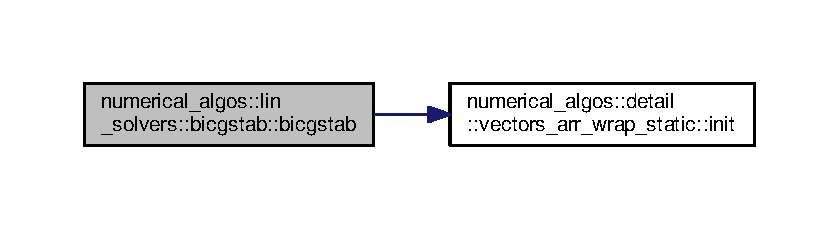
\includegraphics[width=350pt]{classnumerical__algos_1_1lin__solvers_1_1bicgstab_a2ef7808628f564b8cdc9aed0f108ebda_cgraph}
\end{center}
\end{figure}


\hypertarget{classnumerical__algos_1_1lin__solvers_1_1bicgstab_ae84e9e1ede472200f7f2ca5eacbb4389}{\index{numerical\-\_\-algos\-::lin\-\_\-solvers\-::bicgstab@{numerical\-\_\-algos\-::lin\-\_\-solvers\-::bicgstab}!$\sim$bicgstab@{$\sim$bicgstab}}
\index{$\sim$bicgstab@{$\sim$bicgstab}!numerical_algos::lin_solvers::bicgstab@{numerical\-\_\-algos\-::lin\-\_\-solvers\-::bicgstab}}
\subsubsection[{$\sim$bicgstab}]{\setlength{\rightskip}{0pt plus 5cm}template$<$class Linear\-Operator , class Preconditioner , class Vector\-Operations , class Monitor , class Log $>$ {\bf numerical\-\_\-algos\-::lin\-\_\-solvers\-::bicgstab}$<$ Linear\-Operator, Preconditioner, Vector\-Operations, Monitor, Log $>$\-::$\sim${\bf bicgstab} (
\begin{DoxyParamCaption}
{}
\end{DoxyParamCaption}
)\hspace{0.3cm}{\ttfamily [inline]}}}\label{classnumerical__algos_1_1lin__solvers_1_1bicgstab_ae84e9e1ede472200f7f2ca5eacbb4389}
\hypertarget{classnumerical__algos_1_1lin__solvers_1_1bicgstab_a2ef7808628f564b8cdc9aed0f108ebda}{\index{numerical\-\_\-algos\-::lin\-\_\-solvers\-::bicgstab@{numerical\-\_\-algos\-::lin\-\_\-solvers\-::bicgstab}!bicgstab@{bicgstab}}
\index{bicgstab@{bicgstab}!numerical_algos::lin_solvers::bicgstab@{numerical\-\_\-algos\-::lin\-\_\-solvers\-::bicgstab}}
\subsubsection[{bicgstab}]{\setlength{\rightskip}{0pt plus 5cm}template$<$class Linear\-Operator , class Preconditioner , class Vector\-Operations , class Monitor , class Log $>$ {\bf numerical\-\_\-algos\-::lin\-\_\-solvers\-::bicgstab}$<$ Linear\-Operator, Preconditioner, Vector\-Operations, Monitor, Log $>$\-::{\bf bicgstab} (
\begin{DoxyParamCaption}
\item[{const {\bf vector\-\_\-operations\-\_\-type} $\ast$}]{vec\-\_\-ops, }
\item[{Log $\ast$}]{log = {\ttfamily NULL}, }
\item[{{\bf int}}]{obj\-\_\-log\-\_\-lev = {\ttfamily 0}}
\end{DoxyParamCaption}
)\hspace{0.3cm}{\ttfamily [inline]}}}\label{classnumerical__algos_1_1lin__solvers_1_1bicgstab_a2ef7808628f564b8cdc9aed0f108ebda}


Here is the call graph for this function\-:
\nopagebreak
\begin{figure}[H]
\begin{center}
\leavevmode
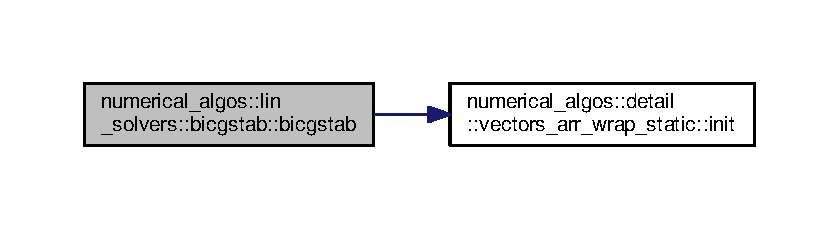
\includegraphics[width=350pt]{classnumerical__algos_1_1lin__solvers_1_1bicgstab_a2ef7808628f564b8cdc9aed0f108ebda_cgraph}
\end{center}
\end{figure}




\subsection{Member Function Documentation}
\hypertarget{classnumerical__algos_1_1lin__solvers_1_1bicgstab_a9f90b0901edd43e3c67d900688e436d3}{\index{numerical\-\_\-algos\-::lin\-\_\-solvers\-::bicgstab@{numerical\-\_\-algos\-::lin\-\_\-solvers\-::bicgstab}!set\-\_\-resid\-\_\-recalc\-\_\-freq@{set\-\_\-resid\-\_\-recalc\-\_\-freq}}
\index{set\-\_\-resid\-\_\-recalc\-\_\-freq@{set\-\_\-resid\-\_\-recalc\-\_\-freq}!numerical_algos::lin_solvers::bicgstab@{numerical\-\_\-algos\-::lin\-\_\-solvers\-::bicgstab}}
\subsubsection[{set\-\_\-resid\-\_\-recalc\-\_\-freq}]{\setlength{\rightskip}{0pt plus 5cm}template$<$class Linear\-Operator , class Preconditioner , class Vector\-Operations , class Monitor , class Log $>$ void {\bf numerical\-\_\-algos\-::lin\-\_\-solvers\-::bicgstab}$<$ Linear\-Operator, Preconditioner, Vector\-Operations, Monitor, Log $>$\-::set\-\_\-resid\-\_\-recalc\-\_\-freq (
\begin{DoxyParamCaption}
\item[{{\bf int}}]{resid\-\_\-recalc\-\_\-freq}
\end{DoxyParamCaption}
)\hspace{0.3cm}{\ttfamily [inline]}}}\label{classnumerical__algos_1_1lin__solvers_1_1bicgstab_a9f90b0901edd43e3c67d900688e436d3}


Here is the caller graph for this function\-:
\nopagebreak
\begin{figure}[H]
\begin{center}
\leavevmode
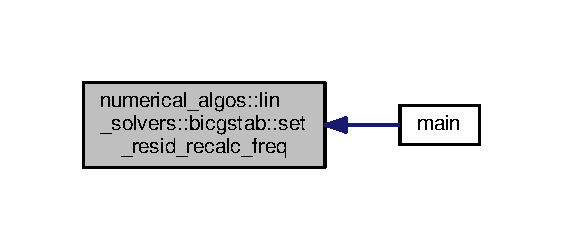
\includegraphics[width=270pt]{classnumerical__algos_1_1lin__solvers_1_1bicgstab_a9f90b0901edd43e3c67d900688e436d3_icgraph}
\end{center}
\end{figure}


\hypertarget{classnumerical__algos_1_1lin__solvers_1_1bicgstab_a61ef325066d9edb6529fb1fca673d6c1}{\index{numerical\-\_\-algos\-::lin\-\_\-solvers\-::bicgstab@{numerical\-\_\-algos\-::lin\-\_\-solvers\-::bicgstab}!set\-\_\-use\-\_\-precond\-\_\-resid@{set\-\_\-use\-\_\-precond\-\_\-resid}}
\index{set\-\_\-use\-\_\-precond\-\_\-resid@{set\-\_\-use\-\_\-precond\-\_\-resid}!numerical_algos::lin_solvers::bicgstab@{numerical\-\_\-algos\-::lin\-\_\-solvers\-::bicgstab}}
\subsubsection[{set\-\_\-use\-\_\-precond\-\_\-resid}]{\setlength{\rightskip}{0pt plus 5cm}template$<$class Linear\-Operator , class Preconditioner , class Vector\-Operations , class Monitor , class Log $>$ void {\bf numerical\-\_\-algos\-::lin\-\_\-solvers\-::bicgstab}$<$ Linear\-Operator, Preconditioner, Vector\-Operations, Monitor, Log $>$\-::set\-\_\-use\-\_\-precond\-\_\-resid (
\begin{DoxyParamCaption}
\item[{bool}]{use\-\_\-precond\-\_\-resid}
\end{DoxyParamCaption}
)\hspace{0.3cm}{\ttfamily [inline]}}}\label{classnumerical__algos_1_1lin__solvers_1_1bicgstab_a61ef325066d9edb6529fb1fca673d6c1}
\hypertarget{classnumerical__algos_1_1lin__solvers_1_1bicgstab_a61ef325066d9edb6529fb1fca673d6c1}{\index{numerical\-\_\-algos\-::lin\-\_\-solvers\-::bicgstab@{numerical\-\_\-algos\-::lin\-\_\-solvers\-::bicgstab}!set\-\_\-use\-\_\-precond\-\_\-resid@{set\-\_\-use\-\_\-precond\-\_\-resid}}
\index{set\-\_\-use\-\_\-precond\-\_\-resid@{set\-\_\-use\-\_\-precond\-\_\-resid}!numerical_algos::lin_solvers::bicgstab@{numerical\-\_\-algos\-::lin\-\_\-solvers\-::bicgstab}}
\subsubsection[{set\-\_\-use\-\_\-precond\-\_\-resid}]{\setlength{\rightskip}{0pt plus 5cm}template$<$class Linear\-Operator , class Preconditioner , class Vector\-Operations , class Monitor , class Log $>$ void {\bf numerical\-\_\-algos\-::lin\-\_\-solvers\-::bicgstab}$<$ Linear\-Operator, Preconditioner, Vector\-Operations, Monitor, Log $>$\-::set\-\_\-use\-\_\-precond\-\_\-resid (
\begin{DoxyParamCaption}
\item[{bool}]{use\-\_\-precond\-\_\-resid}
\end{DoxyParamCaption}
)\hspace{0.3cm}{\ttfamily [inline]}}}\label{classnumerical__algos_1_1lin__solvers_1_1bicgstab_a61ef325066d9edb6529fb1fca673d6c1}


Here is the caller graph for this function\-:
\nopagebreak
\begin{figure}[H]
\begin{center}
\leavevmode
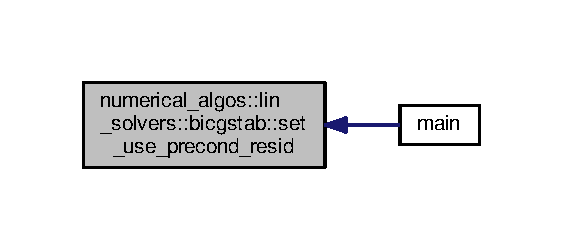
\includegraphics[width=270pt]{classnumerical__algos_1_1lin__solvers_1_1bicgstab_a61ef325066d9edb6529fb1fca673d6c1_icgraph}
\end{center}
\end{figure}


\hypertarget{classnumerical__algos_1_1lin__solvers_1_1bicgstab_ae69b7e9da24cba334a330781d0f00c98}{\index{numerical\-\_\-algos\-::lin\-\_\-solvers\-::bicgstab@{numerical\-\_\-algos\-::lin\-\_\-solvers\-::bicgstab}!set\-\_\-use\-\_\-real\-\_\-resid@{set\-\_\-use\-\_\-real\-\_\-resid}}
\index{set\-\_\-use\-\_\-real\-\_\-resid@{set\-\_\-use\-\_\-real\-\_\-resid}!numerical_algos::lin_solvers::bicgstab@{numerical\-\_\-algos\-::lin\-\_\-solvers\-::bicgstab}}
\subsubsection[{set\-\_\-use\-\_\-real\-\_\-resid}]{\setlength{\rightskip}{0pt plus 5cm}template$<$class Linear\-Operator , class Preconditioner , class Vector\-Operations , class Monitor , class Log $>$ void {\bf numerical\-\_\-algos\-::lin\-\_\-solvers\-::bicgstab}$<$ Linear\-Operator, Preconditioner, Vector\-Operations, Monitor, Log $>$\-::set\-\_\-use\-\_\-real\-\_\-resid (
\begin{DoxyParamCaption}
\item[{bool}]{use\-\_\-real\-\_\-resid}
\end{DoxyParamCaption}
)\hspace{0.3cm}{\ttfamily [inline]}}}\label{classnumerical__algos_1_1lin__solvers_1_1bicgstab_ae69b7e9da24cba334a330781d0f00c98}


Here is the caller graph for this function\-:
\nopagebreak
\begin{figure}[H]
\begin{center}
\leavevmode
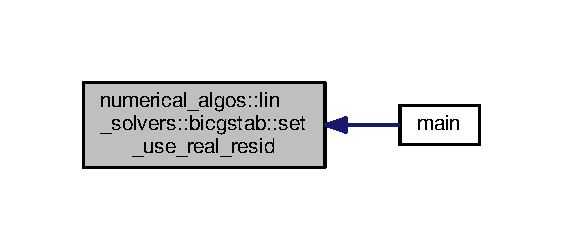
\includegraphics[width=270pt]{classnumerical__algos_1_1lin__solvers_1_1bicgstab_ae69b7e9da24cba334a330781d0f00c98_icgraph}
\end{center}
\end{figure}


\hypertarget{classnumerical__algos_1_1lin__solvers_1_1bicgstab_ac3df95058825e4a8a1ed6bf838f10669}{\index{numerical\-\_\-algos\-::lin\-\_\-solvers\-::bicgstab@{numerical\-\_\-algos\-::lin\-\_\-solvers\-::bicgstab}!solve@{solve}}
\index{solve@{solve}!numerical_algos::lin_solvers::bicgstab@{numerical\-\_\-algos\-::lin\-\_\-solvers\-::bicgstab}}
\subsubsection[{solve}]{\setlength{\rightskip}{0pt plus 5cm}template$<$class Linear\-Operator , class Preconditioner , class Vector\-Operations , class Monitor , class Log $>$ virtual bool {\bf numerical\-\_\-algos\-::lin\-\_\-solvers\-::bicgstab}$<$ Linear\-Operator, Preconditioner, Vector\-Operations, Monitor, Log $>$\-::solve (
\begin{DoxyParamCaption}
\item[{const {\bf linear\-\_\-operator\-\_\-type} \&}]{A, }
\item[{const {\bf vector\-\_\-type} \&}]{b, }
\item[{{\bf vector\-\_\-type} \&}]{x}
\end{DoxyParamCaption}
) const\hspace{0.3cm}{\ttfamily [inline]}, {\ttfamily [virtual]}}}\label{classnumerical__algos_1_1lin__solvers_1_1bicgstab_ac3df95058825e4a8a1ed6bf838f10669}


Implements \hyperlink{classnumerical__algos_1_1lin__solvers_1_1iter__solver__base_ac21be1f601f4937a97c0d3df3182a2af}{numerical\-\_\-algos\-::lin\-\_\-solvers\-::iter\-\_\-solver\-\_\-base$<$ Linear\-Operator, Preconditioner, Vector\-Operations, Monitor, Log $>$}.



Here is the call graph for this function\-:
\nopagebreak
\begin{figure}[H]
\begin{center}
\leavevmode
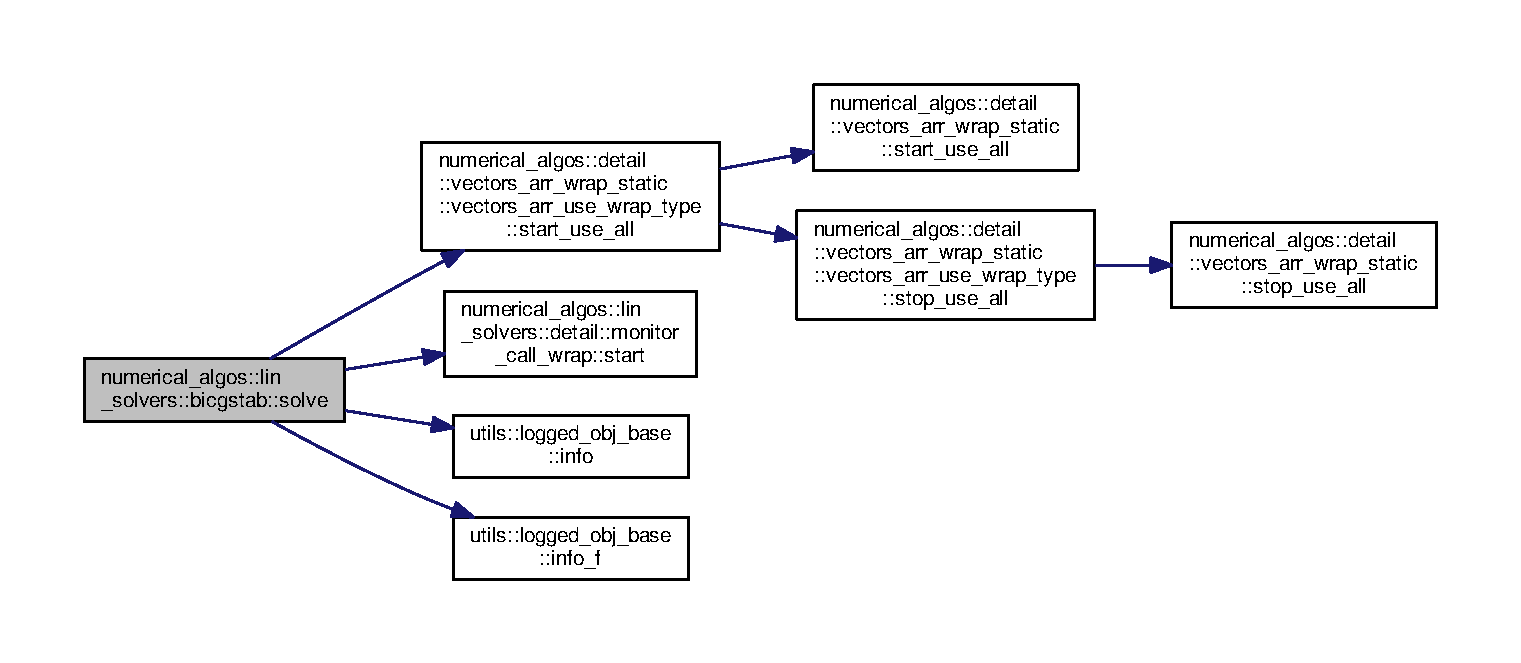
\includegraphics[width=350pt]{classnumerical__algos_1_1lin__solvers_1_1bicgstab_ac3df95058825e4a8a1ed6bf838f10669_cgraph}
\end{center}
\end{figure}


\hypertarget{classnumerical__algos_1_1lin__solvers_1_1bicgstab_ac3df95058825e4a8a1ed6bf838f10669}{\index{numerical\-\_\-algos\-::lin\-\_\-solvers\-::bicgstab@{numerical\-\_\-algos\-::lin\-\_\-solvers\-::bicgstab}!solve@{solve}}
\index{solve@{solve}!numerical_algos::lin_solvers::bicgstab@{numerical\-\_\-algos\-::lin\-\_\-solvers\-::bicgstab}}
\subsubsection[{solve}]{\setlength{\rightskip}{0pt plus 5cm}template$<$class Linear\-Operator , class Preconditioner , class Vector\-Operations , class Monitor , class Log $>$ virtual bool {\bf numerical\-\_\-algos\-::lin\-\_\-solvers\-::bicgstab}$<$ Linear\-Operator, Preconditioner, Vector\-Operations, Monitor, Log $>$\-::solve (
\begin{DoxyParamCaption}
\item[{const {\bf linear\-\_\-operator\-\_\-type} \&}]{A, }
\item[{const {\bf vector\-\_\-type} \&}]{b, }
\item[{{\bf vector\-\_\-type} \&}]{x}
\end{DoxyParamCaption}
) const\hspace{0.3cm}{\ttfamily [inline]}, {\ttfamily [virtual]}}}\label{classnumerical__algos_1_1lin__solvers_1_1bicgstab_ac3df95058825e4a8a1ed6bf838f10669}


Implements \hyperlink{classnumerical__algos_1_1lin__solvers_1_1iter__solver__base_ac21be1f601f4937a97c0d3df3182a2af}{numerical\-\_\-algos\-::lin\-\_\-solvers\-::iter\-\_\-solver\-\_\-base$<$ Linear\-Operator, Preconditioner, Vector\-Operations, Monitor, Log $>$}.



Here is the call graph for this function\-:
\nopagebreak
\begin{figure}[H]
\begin{center}
\leavevmode
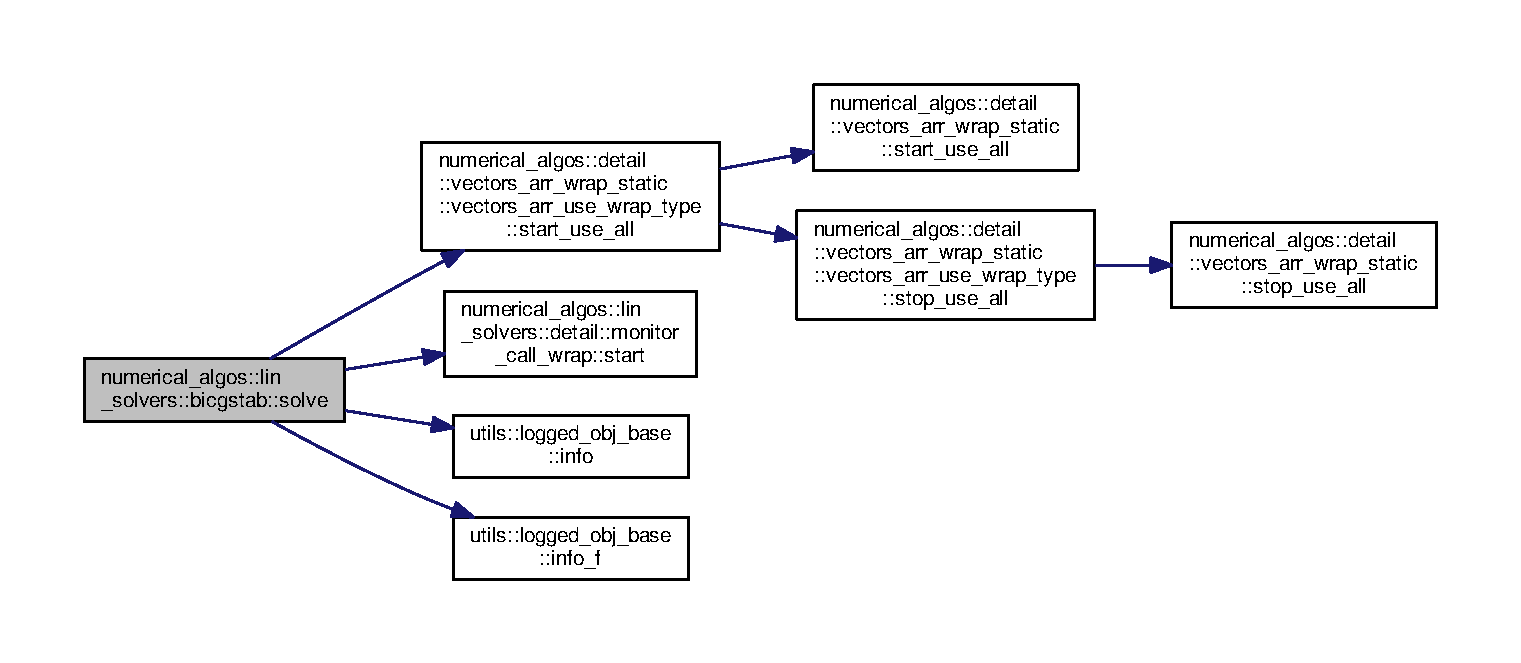
\includegraphics[width=350pt]{classnumerical__algos_1_1lin__solvers_1_1bicgstab_ac3df95058825e4a8a1ed6bf838f10669_cgraph}
\end{center}
\end{figure}




Here is the caller graph for this function\-:
\nopagebreak
\begin{figure}[H]
\begin{center}
\leavevmode
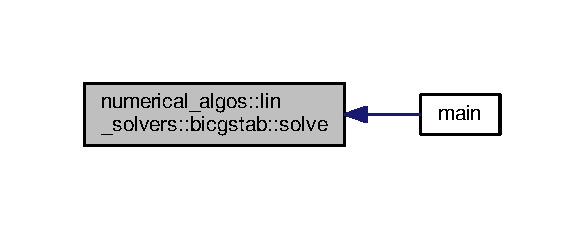
\includegraphics[width=280pt]{classnumerical__algos_1_1lin__solvers_1_1bicgstab_ac3df95058825e4a8a1ed6bf838f10669_icgraph}
\end{center}
\end{figure}




The documentation for this class was generated from the following files\-:\begin{DoxyCompactItemize}
\item 
source/numerical\-\_\-algos/lin\-\_\-solvers/\hyperlink{bicgstab_8h}{bicgstab.\-h}\item 
source/numerical\-\_\-algos/lin\-\_\-solvers/\hyperlink{bicgstab__real__resid_8h}{bicgstab\-\_\-real\-\_\-resid.\-h}\end{DoxyCompactItemize}

\hypertarget{classnumerical__algos_1_1lin__solvers_1_1bicgstabl}{\section{numerical\-\_\-algos\-:\-:lin\-\_\-solvers\-:\-:bicgstabl$<$ Linear\-Operator, Preconditioner, Vector\-Operations, Monitor, Log $>$ Class Template Reference}
\label{classnumerical__algos_1_1lin__solvers_1_1bicgstabl}\index{numerical\-\_\-algos\-::lin\-\_\-solvers\-::bicgstabl$<$ Linear\-Operator, Preconditioner, Vector\-Operations, Monitor, Log $>$@{numerical\-\_\-algos\-::lin\-\_\-solvers\-::bicgstabl$<$ Linear\-Operator, Preconditioner, Vector\-Operations, Monitor, Log $>$}}
}


{\ttfamily \#include $<$bicgstabl.\-h$>$}



Inheritance diagram for numerical\-\_\-algos\-:\-:lin\-\_\-solvers\-:\-:bicgstabl$<$ Linear\-Operator, Preconditioner, Vector\-Operations, Monitor, Log $>$\-:
\nopagebreak
\begin{figure}[H]
\begin{center}
\leavevmode
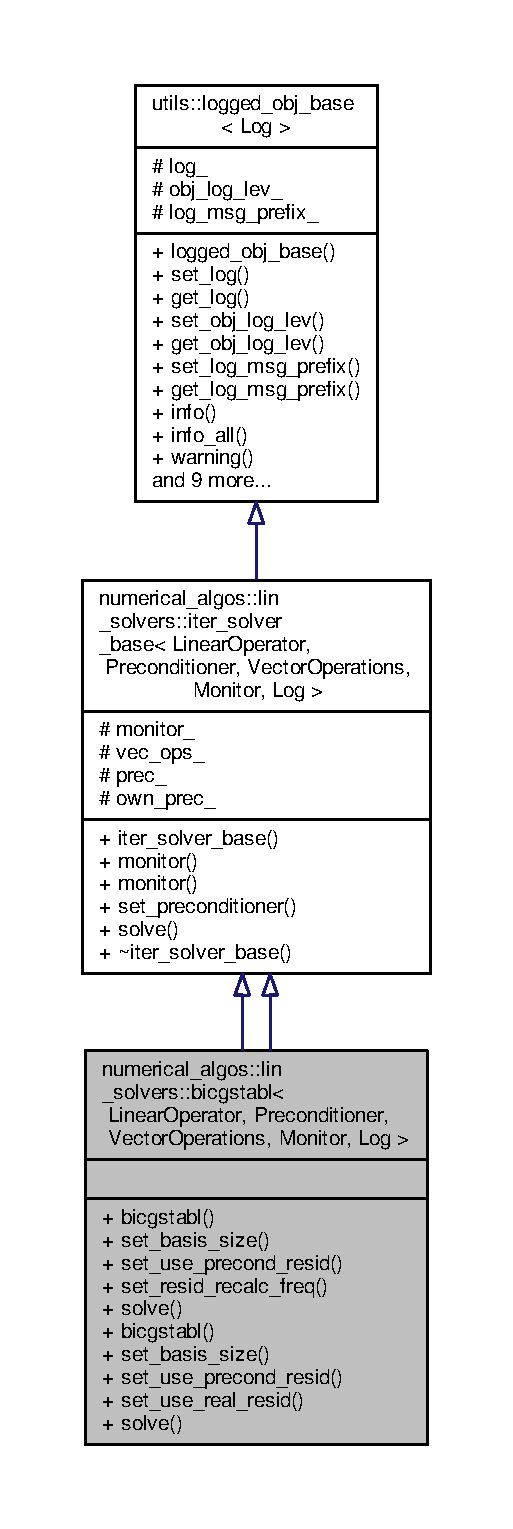
\includegraphics[height=550pt]{classnumerical__algos_1_1lin__solvers_1_1bicgstabl__inherit__graph}
\end{center}
\end{figure}


Collaboration diagram for numerical\-\_\-algos\-:\-:lin\-\_\-solvers\-:\-:bicgstabl$<$ Linear\-Operator, Preconditioner, Vector\-Operations, Monitor, Log $>$\-:
\nopagebreak
\begin{figure}[H]
\begin{center}
\leavevmode
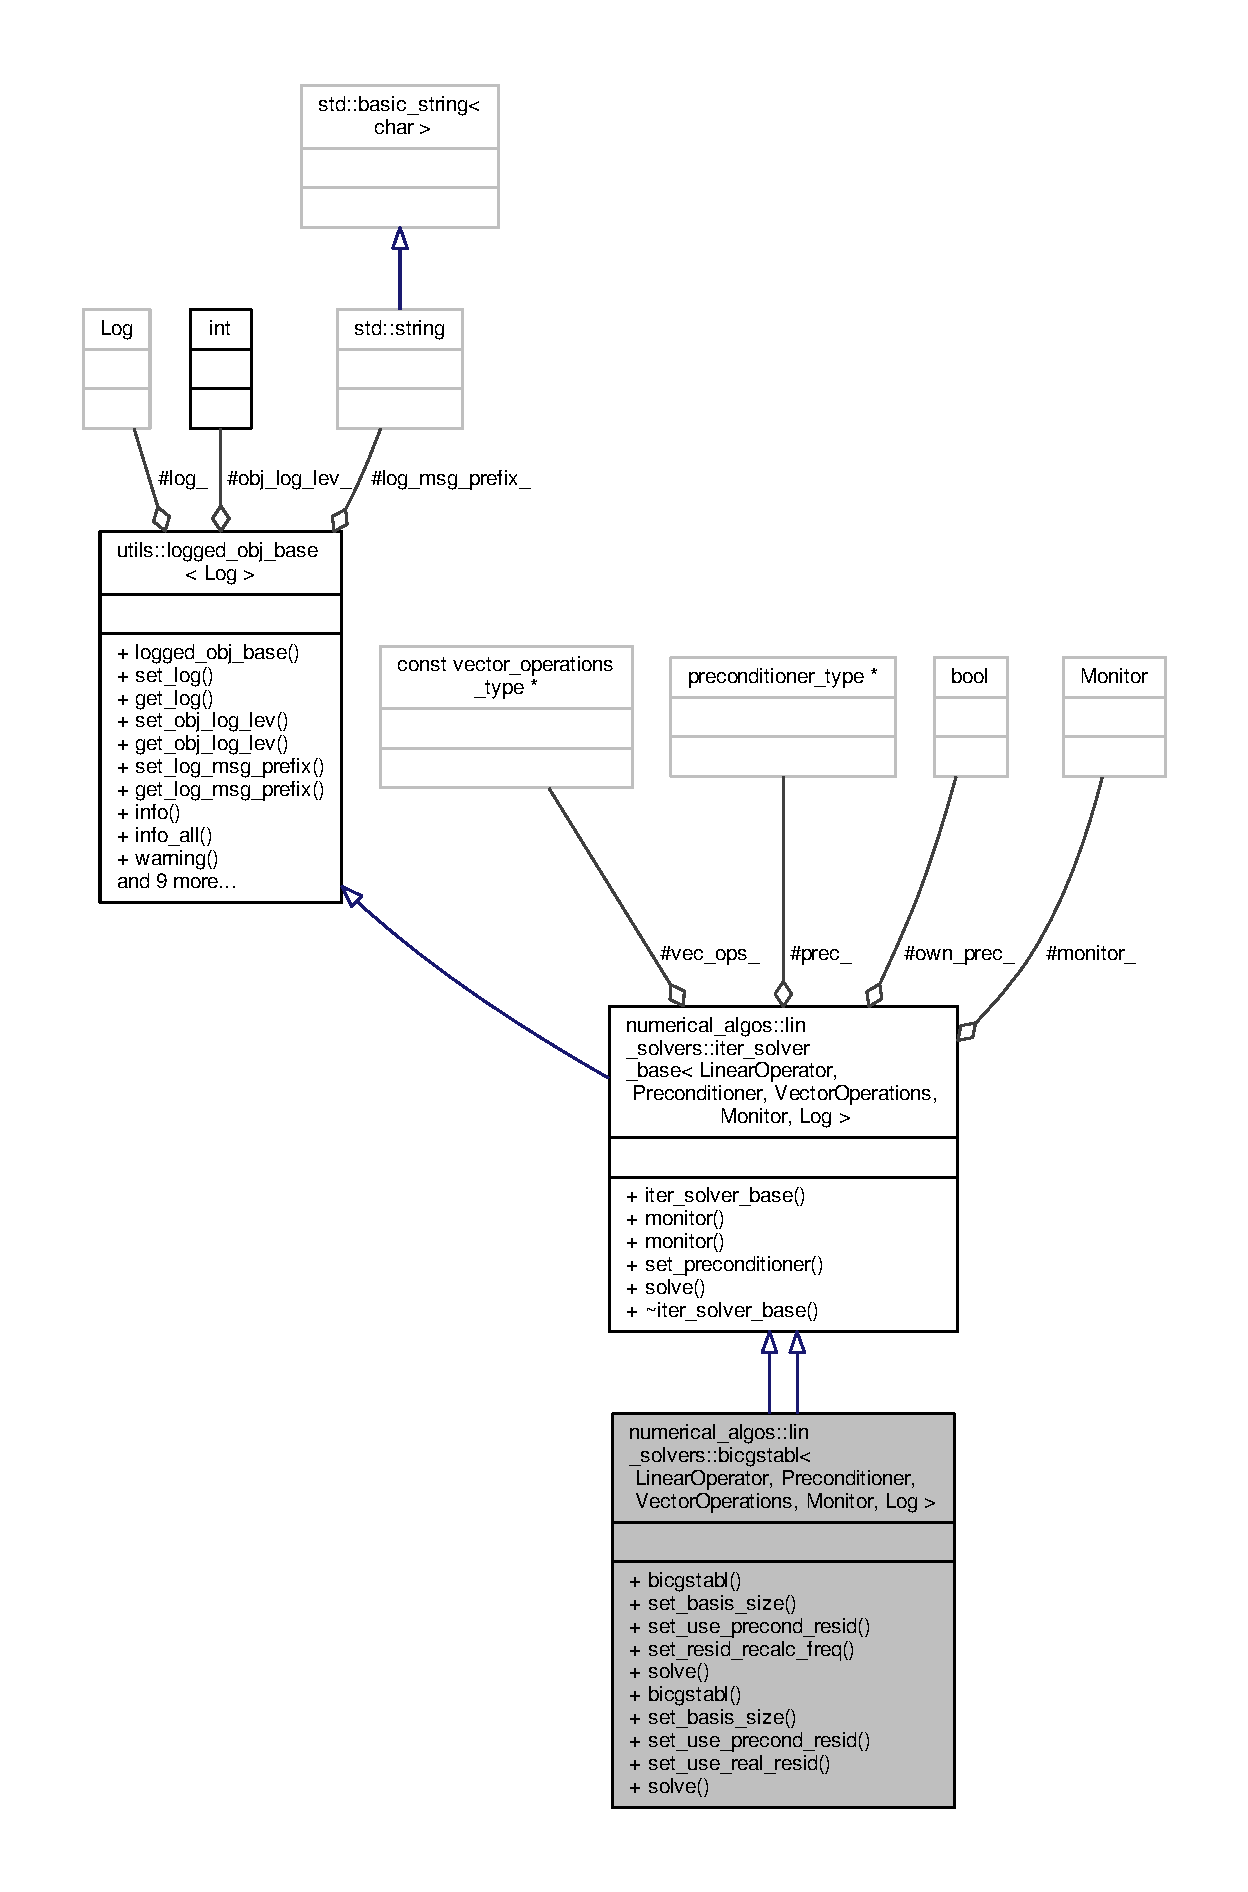
\includegraphics[width=350pt]{classnumerical__algos_1_1lin__solvers_1_1bicgstabl__coll__graph}
\end{center}
\end{figure}
\subsection*{Public Types}
\begin{DoxyCompactItemize}
\item 
typedef \\*
Vector\-Operations\-::scalar\-\_\-type \hyperlink{classnumerical__algos_1_1lin__solvers_1_1bicgstabl_a2756ac0272be9f905269641d9f74bb8e}{scalar\-\_\-type}
\item 
typedef \\*
Vector\-Operations\-::vector\-\_\-type \hyperlink{classnumerical__algos_1_1lin__solvers_1_1bicgstabl_add3b80f2998237878d4cbe24478bcf53}{vector\-\_\-type}
\item 
typedef Linear\-Operator \hyperlink{classnumerical__algos_1_1lin__solvers_1_1bicgstabl_a01e654bee784fc6e5fae7b02dd408523}{linear\-\_\-operator\-\_\-type}
\item 
typedef Preconditioner \hyperlink{classnumerical__algos_1_1lin__solvers_1_1bicgstabl_ae6594eb67e1314591b179bcf6426cd42}{preconditioner\-\_\-type}
\item 
typedef Vector\-Operations \hyperlink{classnumerical__algos_1_1lin__solvers_1_1bicgstabl_a10544b2c65e7fcf5ff71a3049c19734c}{vector\-\_\-operations\-\_\-type}
\item 
typedef Monitor \hyperlink{classnumerical__algos_1_1lin__solvers_1_1bicgstabl_a220cc0b13fdb1f9cbd9dcbfc6aaaccd8}{monitor\-\_\-type}
\item 
typedef Log \hyperlink{classnumerical__algos_1_1lin__solvers_1_1bicgstabl_af655ab52679d5d959cccf86e56a33d63}{log\-\_\-type}
\item 
typedef \\*
Vector\-Operations\-::scalar\-\_\-type \hyperlink{classnumerical__algos_1_1lin__solvers_1_1bicgstabl_a2756ac0272be9f905269641d9f74bb8e}{scalar\-\_\-type}
\item 
typedef \\*
Vector\-Operations\-::vector\-\_\-type \hyperlink{classnumerical__algos_1_1lin__solvers_1_1bicgstabl_add3b80f2998237878d4cbe24478bcf53}{vector\-\_\-type}
\item 
typedef Linear\-Operator \hyperlink{classnumerical__algos_1_1lin__solvers_1_1bicgstabl_a01e654bee784fc6e5fae7b02dd408523}{linear\-\_\-operator\-\_\-type}
\item 
typedef Preconditioner \hyperlink{classnumerical__algos_1_1lin__solvers_1_1bicgstabl_ae6594eb67e1314591b179bcf6426cd42}{preconditioner\-\_\-type}
\item 
typedef Vector\-Operations \hyperlink{classnumerical__algos_1_1lin__solvers_1_1bicgstabl_a10544b2c65e7fcf5ff71a3049c19734c}{vector\-\_\-operations\-\_\-type}
\item 
typedef Monitor \hyperlink{classnumerical__algos_1_1lin__solvers_1_1bicgstabl_a220cc0b13fdb1f9cbd9dcbfc6aaaccd8}{monitor\-\_\-type}
\item 
typedef Log \hyperlink{classnumerical__algos_1_1lin__solvers_1_1bicgstabl_af655ab52679d5d959cccf86e56a33d63}{log\-\_\-type}
\end{DoxyCompactItemize}
\subsection*{Public Member Functions}
\begin{DoxyCompactItemize}
\item 
\hyperlink{classnumerical__algos_1_1lin__solvers_1_1bicgstabl_ab11c8e6fd2099e7b2c7906b8423572b0}{bicgstabl} (const \hyperlink{classnumerical__algos_1_1lin__solvers_1_1bicgstabl_a10544b2c65e7fcf5ff71a3049c19734c}{vector\-\_\-operations\-\_\-type} $\ast$vec\-\_\-ops, Log $\ast$log=N\-U\-L\-L, \hyperlink{classint}{int} obj\-\_\-log\-\_\-lev=0)
\item 
void \hyperlink{classnumerical__algos_1_1lin__solvers_1_1bicgstabl_a358188c0202233c9330fe6a0ec6a8440}{set\-\_\-basis\-\_\-size} (\hyperlink{classint}{int} basis\-\_\-sz)
\item 
void \hyperlink{classnumerical__algos_1_1lin__solvers_1_1bicgstabl_ab420850c21b5e6a86cd41491e309cb56}{set\-\_\-use\-\_\-precond\-\_\-resid} (bool use\-\_\-precond\-\_\-resid)
\item 
void \hyperlink{classnumerical__algos_1_1lin__solvers_1_1bicgstabl_a447c4cc465306db85a804c0e6b2773f4}{set\-\_\-resid\-\_\-recalc\-\_\-freq} (\hyperlink{classint}{int} resid\-\_\-recalc\-\_\-freq)
\item 
virtual bool \hyperlink{classnumerical__algos_1_1lin__solvers_1_1bicgstabl_a2dd4f6cdd207b1a77aa94831fbdf9839}{solve} (const \hyperlink{classnumerical__algos_1_1lin__solvers_1_1bicgstabl_a01e654bee784fc6e5fae7b02dd408523}{linear\-\_\-operator\-\_\-type} \&A, const \hyperlink{classnumerical__algos_1_1lin__solvers_1_1bicgstabl_add3b80f2998237878d4cbe24478bcf53}{vector\-\_\-type} \&b, \hyperlink{classnumerical__algos_1_1lin__solvers_1_1bicgstabl_add3b80f2998237878d4cbe24478bcf53}{vector\-\_\-type} \&x) const 
\item 
\hyperlink{classnumerical__algos_1_1lin__solvers_1_1bicgstabl_ab11c8e6fd2099e7b2c7906b8423572b0}{bicgstabl} (const \hyperlink{classnumerical__algos_1_1lin__solvers_1_1bicgstabl_a10544b2c65e7fcf5ff71a3049c19734c}{vector\-\_\-operations\-\_\-type} $\ast$vec\-\_\-ops, Log $\ast$log=N\-U\-L\-L, \hyperlink{classint}{int} obj\-\_\-log\-\_\-lev=0)
\item 
void \hyperlink{classnumerical__algos_1_1lin__solvers_1_1bicgstabl_a358188c0202233c9330fe6a0ec6a8440}{set\-\_\-basis\-\_\-size} (\hyperlink{classint}{int} basis\-\_\-sz)
\item 
void \hyperlink{classnumerical__algos_1_1lin__solvers_1_1bicgstabl_ab420850c21b5e6a86cd41491e309cb56}{set\-\_\-use\-\_\-precond\-\_\-resid} (bool use\-\_\-precond\-\_\-resid)
\item 
void \hyperlink{classnumerical__algos_1_1lin__solvers_1_1bicgstabl_a384c0d158f1f920be404a0165672965f}{set\-\_\-use\-\_\-real\-\_\-resid} (bool use\-\_\-real\-\_\-resid)
\item 
virtual bool \hyperlink{classnumerical__algos_1_1lin__solvers_1_1bicgstabl_a2dd4f6cdd207b1a77aa94831fbdf9839}{solve} (const \hyperlink{classnumerical__algos_1_1lin__solvers_1_1bicgstabl_a01e654bee784fc6e5fae7b02dd408523}{linear\-\_\-operator\-\_\-type} \&A, const \hyperlink{classnumerical__algos_1_1lin__solvers_1_1bicgstabl_add3b80f2998237878d4cbe24478bcf53}{vector\-\_\-type} \&b, \hyperlink{classnumerical__algos_1_1lin__solvers_1_1bicgstabl_add3b80f2998237878d4cbe24478bcf53}{vector\-\_\-type} \&x) const 
\end{DoxyCompactItemize}
\subsection*{Additional Inherited Members}


\subsection{Member Typedef Documentation}
\hypertarget{classnumerical__algos_1_1lin__solvers_1_1bicgstabl_a01e654bee784fc6e5fae7b02dd408523}{\index{numerical\-\_\-algos\-::lin\-\_\-solvers\-::bicgstabl@{numerical\-\_\-algos\-::lin\-\_\-solvers\-::bicgstabl}!linear\-\_\-operator\-\_\-type@{linear\-\_\-operator\-\_\-type}}
\index{linear\-\_\-operator\-\_\-type@{linear\-\_\-operator\-\_\-type}!numerical_algos::lin_solvers::bicgstabl@{numerical\-\_\-algos\-::lin\-\_\-solvers\-::bicgstabl}}
\subsubsection[{linear\-\_\-operator\-\_\-type}]{\setlength{\rightskip}{0pt plus 5cm}template$<$class Linear\-Operator , class Preconditioner , class Vector\-Operations , class Monitor , class Log $>$ typedef Linear\-Operator {\bf numerical\-\_\-algos\-::lin\-\_\-solvers\-::bicgstabl}$<$ Linear\-Operator, Preconditioner, Vector\-Operations, Monitor, Log $>$\-::{\bf linear\-\_\-operator\-\_\-type}}}\label{classnumerical__algos_1_1lin__solvers_1_1bicgstabl_a01e654bee784fc6e5fae7b02dd408523}
\hypertarget{classnumerical__algos_1_1lin__solvers_1_1bicgstabl_a01e654bee784fc6e5fae7b02dd408523}{\index{numerical\-\_\-algos\-::lin\-\_\-solvers\-::bicgstabl@{numerical\-\_\-algos\-::lin\-\_\-solvers\-::bicgstabl}!linear\-\_\-operator\-\_\-type@{linear\-\_\-operator\-\_\-type}}
\index{linear\-\_\-operator\-\_\-type@{linear\-\_\-operator\-\_\-type}!numerical_algos::lin_solvers::bicgstabl@{numerical\-\_\-algos\-::lin\-\_\-solvers\-::bicgstabl}}
\subsubsection[{linear\-\_\-operator\-\_\-type}]{\setlength{\rightskip}{0pt plus 5cm}template$<$class Linear\-Operator , class Preconditioner , class Vector\-Operations , class Monitor , class Log $>$ typedef Linear\-Operator {\bf numerical\-\_\-algos\-::lin\-\_\-solvers\-::bicgstabl}$<$ Linear\-Operator, Preconditioner, Vector\-Operations, Monitor, Log $>$\-::{\bf linear\-\_\-operator\-\_\-type}}}\label{classnumerical__algos_1_1lin__solvers_1_1bicgstabl_a01e654bee784fc6e5fae7b02dd408523}
\hypertarget{classnumerical__algos_1_1lin__solvers_1_1bicgstabl_af655ab52679d5d959cccf86e56a33d63}{\index{numerical\-\_\-algos\-::lin\-\_\-solvers\-::bicgstabl@{numerical\-\_\-algos\-::lin\-\_\-solvers\-::bicgstabl}!log\-\_\-type@{log\-\_\-type}}
\index{log\-\_\-type@{log\-\_\-type}!numerical_algos::lin_solvers::bicgstabl@{numerical\-\_\-algos\-::lin\-\_\-solvers\-::bicgstabl}}
\subsubsection[{log\-\_\-type}]{\setlength{\rightskip}{0pt plus 5cm}template$<$class Linear\-Operator , class Preconditioner , class Vector\-Operations , class Monitor , class Log $>$ typedef Log {\bf numerical\-\_\-algos\-::lin\-\_\-solvers\-::bicgstabl}$<$ Linear\-Operator, Preconditioner, Vector\-Operations, Monitor, Log $>$\-::{\bf log\-\_\-type}}}\label{classnumerical__algos_1_1lin__solvers_1_1bicgstabl_af655ab52679d5d959cccf86e56a33d63}
\hypertarget{classnumerical__algos_1_1lin__solvers_1_1bicgstabl_af655ab52679d5d959cccf86e56a33d63}{\index{numerical\-\_\-algos\-::lin\-\_\-solvers\-::bicgstabl@{numerical\-\_\-algos\-::lin\-\_\-solvers\-::bicgstabl}!log\-\_\-type@{log\-\_\-type}}
\index{log\-\_\-type@{log\-\_\-type}!numerical_algos::lin_solvers::bicgstabl@{numerical\-\_\-algos\-::lin\-\_\-solvers\-::bicgstabl}}
\subsubsection[{log\-\_\-type}]{\setlength{\rightskip}{0pt plus 5cm}template$<$class Linear\-Operator , class Preconditioner , class Vector\-Operations , class Monitor , class Log $>$ typedef Log {\bf numerical\-\_\-algos\-::lin\-\_\-solvers\-::bicgstabl}$<$ Linear\-Operator, Preconditioner, Vector\-Operations, Monitor, Log $>$\-::{\bf log\-\_\-type}}}\label{classnumerical__algos_1_1lin__solvers_1_1bicgstabl_af655ab52679d5d959cccf86e56a33d63}
\hypertarget{classnumerical__algos_1_1lin__solvers_1_1bicgstabl_a220cc0b13fdb1f9cbd9dcbfc6aaaccd8}{\index{numerical\-\_\-algos\-::lin\-\_\-solvers\-::bicgstabl@{numerical\-\_\-algos\-::lin\-\_\-solvers\-::bicgstabl}!monitor\-\_\-type@{monitor\-\_\-type}}
\index{monitor\-\_\-type@{monitor\-\_\-type}!numerical_algos::lin_solvers::bicgstabl@{numerical\-\_\-algos\-::lin\-\_\-solvers\-::bicgstabl}}
\subsubsection[{monitor\-\_\-type}]{\setlength{\rightskip}{0pt plus 5cm}template$<$class Linear\-Operator , class Preconditioner , class Vector\-Operations , class Monitor , class Log $>$ typedef Monitor {\bf numerical\-\_\-algos\-::lin\-\_\-solvers\-::bicgstabl}$<$ Linear\-Operator, Preconditioner, Vector\-Operations, Monitor, Log $>$\-::{\bf monitor\-\_\-type}}}\label{classnumerical__algos_1_1lin__solvers_1_1bicgstabl_a220cc0b13fdb1f9cbd9dcbfc6aaaccd8}
\hypertarget{classnumerical__algos_1_1lin__solvers_1_1bicgstabl_a220cc0b13fdb1f9cbd9dcbfc6aaaccd8}{\index{numerical\-\_\-algos\-::lin\-\_\-solvers\-::bicgstabl@{numerical\-\_\-algos\-::lin\-\_\-solvers\-::bicgstabl}!monitor\-\_\-type@{monitor\-\_\-type}}
\index{monitor\-\_\-type@{monitor\-\_\-type}!numerical_algos::lin_solvers::bicgstabl@{numerical\-\_\-algos\-::lin\-\_\-solvers\-::bicgstabl}}
\subsubsection[{monitor\-\_\-type}]{\setlength{\rightskip}{0pt plus 5cm}template$<$class Linear\-Operator , class Preconditioner , class Vector\-Operations , class Monitor , class Log $>$ typedef Monitor {\bf numerical\-\_\-algos\-::lin\-\_\-solvers\-::bicgstabl}$<$ Linear\-Operator, Preconditioner, Vector\-Operations, Monitor, Log $>$\-::{\bf monitor\-\_\-type}}}\label{classnumerical__algos_1_1lin__solvers_1_1bicgstabl_a220cc0b13fdb1f9cbd9dcbfc6aaaccd8}
\hypertarget{classnumerical__algos_1_1lin__solvers_1_1bicgstabl_ae6594eb67e1314591b179bcf6426cd42}{\index{numerical\-\_\-algos\-::lin\-\_\-solvers\-::bicgstabl@{numerical\-\_\-algos\-::lin\-\_\-solvers\-::bicgstabl}!preconditioner\-\_\-type@{preconditioner\-\_\-type}}
\index{preconditioner\-\_\-type@{preconditioner\-\_\-type}!numerical_algos::lin_solvers::bicgstabl@{numerical\-\_\-algos\-::lin\-\_\-solvers\-::bicgstabl}}
\subsubsection[{preconditioner\-\_\-type}]{\setlength{\rightskip}{0pt plus 5cm}template$<$class Linear\-Operator , class Preconditioner , class Vector\-Operations , class Monitor , class Log $>$ typedef Preconditioner {\bf numerical\-\_\-algos\-::lin\-\_\-solvers\-::bicgstabl}$<$ Linear\-Operator, Preconditioner, Vector\-Operations, Monitor, Log $>$\-::{\bf preconditioner\-\_\-type}}}\label{classnumerical__algos_1_1lin__solvers_1_1bicgstabl_ae6594eb67e1314591b179bcf6426cd42}
\hypertarget{classnumerical__algos_1_1lin__solvers_1_1bicgstabl_ae6594eb67e1314591b179bcf6426cd42}{\index{numerical\-\_\-algos\-::lin\-\_\-solvers\-::bicgstabl@{numerical\-\_\-algos\-::lin\-\_\-solvers\-::bicgstabl}!preconditioner\-\_\-type@{preconditioner\-\_\-type}}
\index{preconditioner\-\_\-type@{preconditioner\-\_\-type}!numerical_algos::lin_solvers::bicgstabl@{numerical\-\_\-algos\-::lin\-\_\-solvers\-::bicgstabl}}
\subsubsection[{preconditioner\-\_\-type}]{\setlength{\rightskip}{0pt plus 5cm}template$<$class Linear\-Operator , class Preconditioner , class Vector\-Operations , class Monitor , class Log $>$ typedef Preconditioner {\bf numerical\-\_\-algos\-::lin\-\_\-solvers\-::bicgstabl}$<$ Linear\-Operator, Preconditioner, Vector\-Operations, Monitor, Log $>$\-::{\bf preconditioner\-\_\-type}}}\label{classnumerical__algos_1_1lin__solvers_1_1bicgstabl_ae6594eb67e1314591b179bcf6426cd42}
\hypertarget{classnumerical__algos_1_1lin__solvers_1_1bicgstabl_a2756ac0272be9f905269641d9f74bb8e}{\index{numerical\-\_\-algos\-::lin\-\_\-solvers\-::bicgstabl@{numerical\-\_\-algos\-::lin\-\_\-solvers\-::bicgstabl}!scalar\-\_\-type@{scalar\-\_\-type}}
\index{scalar\-\_\-type@{scalar\-\_\-type}!numerical_algos::lin_solvers::bicgstabl@{numerical\-\_\-algos\-::lin\-\_\-solvers\-::bicgstabl}}
\subsubsection[{scalar\-\_\-type}]{\setlength{\rightskip}{0pt plus 5cm}template$<$class Linear\-Operator , class Preconditioner , class Vector\-Operations , class Monitor , class Log $>$ typedef Vector\-Operations\-::scalar\-\_\-type {\bf numerical\-\_\-algos\-::lin\-\_\-solvers\-::bicgstabl}$<$ Linear\-Operator, Preconditioner, Vector\-Operations, Monitor, Log $>$\-::{\bf scalar\-\_\-type}}}\label{classnumerical__algos_1_1lin__solvers_1_1bicgstabl_a2756ac0272be9f905269641d9f74bb8e}
\hypertarget{classnumerical__algos_1_1lin__solvers_1_1bicgstabl_a2756ac0272be9f905269641d9f74bb8e}{\index{numerical\-\_\-algos\-::lin\-\_\-solvers\-::bicgstabl@{numerical\-\_\-algos\-::lin\-\_\-solvers\-::bicgstabl}!scalar\-\_\-type@{scalar\-\_\-type}}
\index{scalar\-\_\-type@{scalar\-\_\-type}!numerical_algos::lin_solvers::bicgstabl@{numerical\-\_\-algos\-::lin\-\_\-solvers\-::bicgstabl}}
\subsubsection[{scalar\-\_\-type}]{\setlength{\rightskip}{0pt plus 5cm}template$<$class Linear\-Operator , class Preconditioner , class Vector\-Operations , class Monitor , class Log $>$ typedef Vector\-Operations\-::scalar\-\_\-type {\bf numerical\-\_\-algos\-::lin\-\_\-solvers\-::bicgstabl}$<$ Linear\-Operator, Preconditioner, Vector\-Operations, Monitor, Log $>$\-::{\bf scalar\-\_\-type}}}\label{classnumerical__algos_1_1lin__solvers_1_1bicgstabl_a2756ac0272be9f905269641d9f74bb8e}
\hypertarget{classnumerical__algos_1_1lin__solvers_1_1bicgstabl_a10544b2c65e7fcf5ff71a3049c19734c}{\index{numerical\-\_\-algos\-::lin\-\_\-solvers\-::bicgstabl@{numerical\-\_\-algos\-::lin\-\_\-solvers\-::bicgstabl}!vector\-\_\-operations\-\_\-type@{vector\-\_\-operations\-\_\-type}}
\index{vector\-\_\-operations\-\_\-type@{vector\-\_\-operations\-\_\-type}!numerical_algos::lin_solvers::bicgstabl@{numerical\-\_\-algos\-::lin\-\_\-solvers\-::bicgstabl}}
\subsubsection[{vector\-\_\-operations\-\_\-type}]{\setlength{\rightskip}{0pt plus 5cm}template$<$class Linear\-Operator , class Preconditioner , class Vector\-Operations , class Monitor , class Log $>$ typedef Vector\-Operations {\bf numerical\-\_\-algos\-::lin\-\_\-solvers\-::bicgstabl}$<$ Linear\-Operator, Preconditioner, Vector\-Operations, Monitor, Log $>$\-::{\bf vector\-\_\-operations\-\_\-type}}}\label{classnumerical__algos_1_1lin__solvers_1_1bicgstabl_a10544b2c65e7fcf5ff71a3049c19734c}
\hypertarget{classnumerical__algos_1_1lin__solvers_1_1bicgstabl_a10544b2c65e7fcf5ff71a3049c19734c}{\index{numerical\-\_\-algos\-::lin\-\_\-solvers\-::bicgstabl@{numerical\-\_\-algos\-::lin\-\_\-solvers\-::bicgstabl}!vector\-\_\-operations\-\_\-type@{vector\-\_\-operations\-\_\-type}}
\index{vector\-\_\-operations\-\_\-type@{vector\-\_\-operations\-\_\-type}!numerical_algos::lin_solvers::bicgstabl@{numerical\-\_\-algos\-::lin\-\_\-solvers\-::bicgstabl}}
\subsubsection[{vector\-\_\-operations\-\_\-type}]{\setlength{\rightskip}{0pt plus 5cm}template$<$class Linear\-Operator , class Preconditioner , class Vector\-Operations , class Monitor , class Log $>$ typedef Vector\-Operations {\bf numerical\-\_\-algos\-::lin\-\_\-solvers\-::bicgstabl}$<$ Linear\-Operator, Preconditioner, Vector\-Operations, Monitor, Log $>$\-::{\bf vector\-\_\-operations\-\_\-type}}}\label{classnumerical__algos_1_1lin__solvers_1_1bicgstabl_a10544b2c65e7fcf5ff71a3049c19734c}
\hypertarget{classnumerical__algos_1_1lin__solvers_1_1bicgstabl_add3b80f2998237878d4cbe24478bcf53}{\index{numerical\-\_\-algos\-::lin\-\_\-solvers\-::bicgstabl@{numerical\-\_\-algos\-::lin\-\_\-solvers\-::bicgstabl}!vector\-\_\-type@{vector\-\_\-type}}
\index{vector\-\_\-type@{vector\-\_\-type}!numerical_algos::lin_solvers::bicgstabl@{numerical\-\_\-algos\-::lin\-\_\-solvers\-::bicgstabl}}
\subsubsection[{vector\-\_\-type}]{\setlength{\rightskip}{0pt plus 5cm}template$<$class Linear\-Operator , class Preconditioner , class Vector\-Operations , class Monitor , class Log $>$ typedef Vector\-Operations\-::vector\-\_\-type {\bf numerical\-\_\-algos\-::lin\-\_\-solvers\-::bicgstabl}$<$ Linear\-Operator, Preconditioner, Vector\-Operations, Monitor, Log $>$\-::{\bf vector\-\_\-type}}}\label{classnumerical__algos_1_1lin__solvers_1_1bicgstabl_add3b80f2998237878d4cbe24478bcf53}
\hypertarget{classnumerical__algos_1_1lin__solvers_1_1bicgstabl_add3b80f2998237878d4cbe24478bcf53}{\index{numerical\-\_\-algos\-::lin\-\_\-solvers\-::bicgstabl@{numerical\-\_\-algos\-::lin\-\_\-solvers\-::bicgstabl}!vector\-\_\-type@{vector\-\_\-type}}
\index{vector\-\_\-type@{vector\-\_\-type}!numerical_algos::lin_solvers::bicgstabl@{numerical\-\_\-algos\-::lin\-\_\-solvers\-::bicgstabl}}
\subsubsection[{vector\-\_\-type}]{\setlength{\rightskip}{0pt plus 5cm}template$<$class Linear\-Operator , class Preconditioner , class Vector\-Operations , class Monitor , class Log $>$ typedef Vector\-Operations\-::vector\-\_\-type {\bf numerical\-\_\-algos\-::lin\-\_\-solvers\-::bicgstabl}$<$ Linear\-Operator, Preconditioner, Vector\-Operations, Monitor, Log $>$\-::{\bf vector\-\_\-type}}}\label{classnumerical__algos_1_1lin__solvers_1_1bicgstabl_add3b80f2998237878d4cbe24478bcf53}


\subsection{Constructor \& Destructor Documentation}
\hypertarget{classnumerical__algos_1_1lin__solvers_1_1bicgstabl_ab11c8e6fd2099e7b2c7906b8423572b0}{\index{numerical\-\_\-algos\-::lin\-\_\-solvers\-::bicgstabl@{numerical\-\_\-algos\-::lin\-\_\-solvers\-::bicgstabl}!bicgstabl@{bicgstabl}}
\index{bicgstabl@{bicgstabl}!numerical_algos::lin_solvers::bicgstabl@{numerical\-\_\-algos\-::lin\-\_\-solvers\-::bicgstabl}}
\subsubsection[{bicgstabl}]{\setlength{\rightskip}{0pt plus 5cm}template$<$class Linear\-Operator , class Preconditioner , class Vector\-Operations , class Monitor , class Log $>$ {\bf numerical\-\_\-algos\-::lin\-\_\-solvers\-::bicgstabl}$<$ Linear\-Operator, Preconditioner, Vector\-Operations, Monitor, Log $>$\-::{\bf bicgstabl} (
\begin{DoxyParamCaption}
\item[{const {\bf vector\-\_\-operations\-\_\-type} $\ast$}]{vec\-\_\-ops, }
\item[{Log $\ast$}]{log = {\ttfamily NULL}, }
\item[{{\bf int}}]{obj\-\_\-log\-\_\-lev = {\ttfamily 0}}
\end{DoxyParamCaption}
)\hspace{0.3cm}{\ttfamily [inline]}}}\label{classnumerical__algos_1_1lin__solvers_1_1bicgstabl_ab11c8e6fd2099e7b2c7906b8423572b0}


Here is the call graph for this function\-:
\nopagebreak
\begin{figure}[H]
\begin{center}
\leavevmode
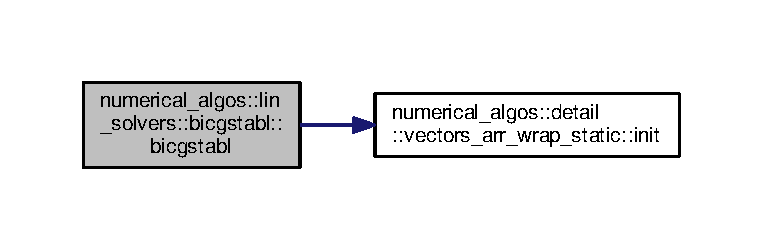
\includegraphics[width=350pt]{classnumerical__algos_1_1lin__solvers_1_1bicgstabl_ab11c8e6fd2099e7b2c7906b8423572b0_cgraph}
\end{center}
\end{figure}


\hypertarget{classnumerical__algos_1_1lin__solvers_1_1bicgstabl_ab11c8e6fd2099e7b2c7906b8423572b0}{\index{numerical\-\_\-algos\-::lin\-\_\-solvers\-::bicgstabl@{numerical\-\_\-algos\-::lin\-\_\-solvers\-::bicgstabl}!bicgstabl@{bicgstabl}}
\index{bicgstabl@{bicgstabl}!numerical_algos::lin_solvers::bicgstabl@{numerical\-\_\-algos\-::lin\-\_\-solvers\-::bicgstabl}}
\subsubsection[{bicgstabl}]{\setlength{\rightskip}{0pt plus 5cm}template$<$class Linear\-Operator , class Preconditioner , class Vector\-Operations , class Monitor , class Log $>$ {\bf numerical\-\_\-algos\-::lin\-\_\-solvers\-::bicgstabl}$<$ Linear\-Operator, Preconditioner, Vector\-Operations, Monitor, Log $>$\-::{\bf bicgstabl} (
\begin{DoxyParamCaption}
\item[{const {\bf vector\-\_\-operations\-\_\-type} $\ast$}]{vec\-\_\-ops, }
\item[{Log $\ast$}]{log = {\ttfamily NULL}, }
\item[{{\bf int}}]{obj\-\_\-log\-\_\-lev = {\ttfamily 0}}
\end{DoxyParamCaption}
)\hspace{0.3cm}{\ttfamily [inline]}}}\label{classnumerical__algos_1_1lin__solvers_1_1bicgstabl_ab11c8e6fd2099e7b2c7906b8423572b0}


Here is the call graph for this function\-:
\nopagebreak
\begin{figure}[H]
\begin{center}
\leavevmode
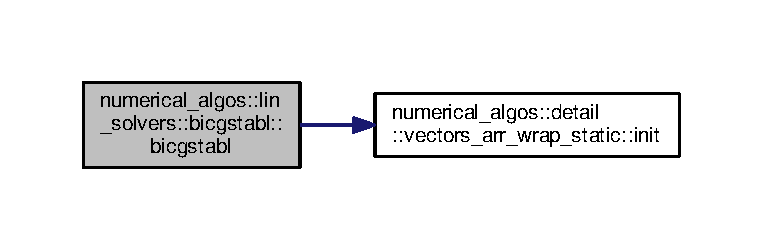
\includegraphics[width=350pt]{classnumerical__algos_1_1lin__solvers_1_1bicgstabl_ab11c8e6fd2099e7b2c7906b8423572b0_cgraph}
\end{center}
\end{figure}




\subsection{Member Function Documentation}
\hypertarget{classnumerical__algos_1_1lin__solvers_1_1bicgstabl_a358188c0202233c9330fe6a0ec6a8440}{\index{numerical\-\_\-algos\-::lin\-\_\-solvers\-::bicgstabl@{numerical\-\_\-algos\-::lin\-\_\-solvers\-::bicgstabl}!set\-\_\-basis\-\_\-size@{set\-\_\-basis\-\_\-size}}
\index{set\-\_\-basis\-\_\-size@{set\-\_\-basis\-\_\-size}!numerical_algos::lin_solvers::bicgstabl@{numerical\-\_\-algos\-::lin\-\_\-solvers\-::bicgstabl}}
\subsubsection[{set\-\_\-basis\-\_\-size}]{\setlength{\rightskip}{0pt plus 5cm}template$<$class Linear\-Operator , class Preconditioner , class Vector\-Operations , class Monitor , class Log $>$ void {\bf numerical\-\_\-algos\-::lin\-\_\-solvers\-::bicgstabl}$<$ Linear\-Operator, Preconditioner, Vector\-Operations, Monitor, Log $>$\-::set\-\_\-basis\-\_\-size (
\begin{DoxyParamCaption}
\item[{{\bf int}}]{basis\-\_\-sz}
\end{DoxyParamCaption}
)\hspace{0.3cm}{\ttfamily [inline]}}}\label{classnumerical__algos_1_1lin__solvers_1_1bicgstabl_a358188c0202233c9330fe6a0ec6a8440}
\hypertarget{classnumerical__algos_1_1lin__solvers_1_1bicgstabl_a358188c0202233c9330fe6a0ec6a8440}{\index{numerical\-\_\-algos\-::lin\-\_\-solvers\-::bicgstabl@{numerical\-\_\-algos\-::lin\-\_\-solvers\-::bicgstabl}!set\-\_\-basis\-\_\-size@{set\-\_\-basis\-\_\-size}}
\index{set\-\_\-basis\-\_\-size@{set\-\_\-basis\-\_\-size}!numerical_algos::lin_solvers::bicgstabl@{numerical\-\_\-algos\-::lin\-\_\-solvers\-::bicgstabl}}
\subsubsection[{set\-\_\-basis\-\_\-size}]{\setlength{\rightskip}{0pt plus 5cm}template$<$class Linear\-Operator , class Preconditioner , class Vector\-Operations , class Monitor , class Log $>$ void {\bf numerical\-\_\-algos\-::lin\-\_\-solvers\-::bicgstabl}$<$ Linear\-Operator, Preconditioner, Vector\-Operations, Monitor, Log $>$\-::set\-\_\-basis\-\_\-size (
\begin{DoxyParamCaption}
\item[{{\bf int}}]{basis\-\_\-sz}
\end{DoxyParamCaption}
)\hspace{0.3cm}{\ttfamily [inline]}}}\label{classnumerical__algos_1_1lin__solvers_1_1bicgstabl_a358188c0202233c9330fe6a0ec6a8440}


Here is the caller graph for this function\-:
\nopagebreak
\begin{figure}[H]
\begin{center}
\leavevmode
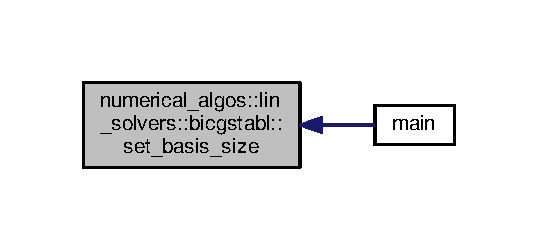
\includegraphics[width=258pt]{classnumerical__algos_1_1lin__solvers_1_1bicgstabl_a358188c0202233c9330fe6a0ec6a8440_icgraph}
\end{center}
\end{figure}


\hypertarget{classnumerical__algos_1_1lin__solvers_1_1bicgstabl_a447c4cc465306db85a804c0e6b2773f4}{\index{numerical\-\_\-algos\-::lin\-\_\-solvers\-::bicgstabl@{numerical\-\_\-algos\-::lin\-\_\-solvers\-::bicgstabl}!set\-\_\-resid\-\_\-recalc\-\_\-freq@{set\-\_\-resid\-\_\-recalc\-\_\-freq}}
\index{set\-\_\-resid\-\_\-recalc\-\_\-freq@{set\-\_\-resid\-\_\-recalc\-\_\-freq}!numerical_algos::lin_solvers::bicgstabl@{numerical\-\_\-algos\-::lin\-\_\-solvers\-::bicgstabl}}
\subsubsection[{set\-\_\-resid\-\_\-recalc\-\_\-freq}]{\setlength{\rightskip}{0pt plus 5cm}template$<$class Linear\-Operator , class Preconditioner , class Vector\-Operations , class Monitor , class Log $>$ void {\bf numerical\-\_\-algos\-::lin\-\_\-solvers\-::bicgstabl}$<$ Linear\-Operator, Preconditioner, Vector\-Operations, Monitor, Log $>$\-::set\-\_\-resid\-\_\-recalc\-\_\-freq (
\begin{DoxyParamCaption}
\item[{{\bf int}}]{resid\-\_\-recalc\-\_\-freq}
\end{DoxyParamCaption}
)\hspace{0.3cm}{\ttfamily [inline]}}}\label{classnumerical__algos_1_1lin__solvers_1_1bicgstabl_a447c4cc465306db85a804c0e6b2773f4}


Here is the caller graph for this function\-:
\nopagebreak
\begin{figure}[H]
\begin{center}
\leavevmode
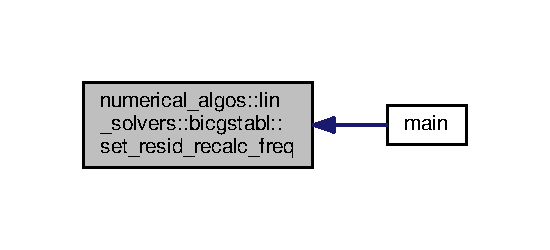
\includegraphics[width=264pt]{classnumerical__algos_1_1lin__solvers_1_1bicgstabl_a447c4cc465306db85a804c0e6b2773f4_icgraph}
\end{center}
\end{figure}


\hypertarget{classnumerical__algos_1_1lin__solvers_1_1bicgstabl_ab420850c21b5e6a86cd41491e309cb56}{\index{numerical\-\_\-algos\-::lin\-\_\-solvers\-::bicgstabl@{numerical\-\_\-algos\-::lin\-\_\-solvers\-::bicgstabl}!set\-\_\-use\-\_\-precond\-\_\-resid@{set\-\_\-use\-\_\-precond\-\_\-resid}}
\index{set\-\_\-use\-\_\-precond\-\_\-resid@{set\-\_\-use\-\_\-precond\-\_\-resid}!numerical_algos::lin_solvers::bicgstabl@{numerical\-\_\-algos\-::lin\-\_\-solvers\-::bicgstabl}}
\subsubsection[{set\-\_\-use\-\_\-precond\-\_\-resid}]{\setlength{\rightskip}{0pt plus 5cm}template$<$class Linear\-Operator , class Preconditioner , class Vector\-Operations , class Monitor , class Log $>$ void {\bf numerical\-\_\-algos\-::lin\-\_\-solvers\-::bicgstabl}$<$ Linear\-Operator, Preconditioner, Vector\-Operations, Monitor, Log $>$\-::set\-\_\-use\-\_\-precond\-\_\-resid (
\begin{DoxyParamCaption}
\item[{bool}]{use\-\_\-precond\-\_\-resid}
\end{DoxyParamCaption}
)\hspace{0.3cm}{\ttfamily [inline]}}}\label{classnumerical__algos_1_1lin__solvers_1_1bicgstabl_ab420850c21b5e6a86cd41491e309cb56}
\hypertarget{classnumerical__algos_1_1lin__solvers_1_1bicgstabl_ab420850c21b5e6a86cd41491e309cb56}{\index{numerical\-\_\-algos\-::lin\-\_\-solvers\-::bicgstabl@{numerical\-\_\-algos\-::lin\-\_\-solvers\-::bicgstabl}!set\-\_\-use\-\_\-precond\-\_\-resid@{set\-\_\-use\-\_\-precond\-\_\-resid}}
\index{set\-\_\-use\-\_\-precond\-\_\-resid@{set\-\_\-use\-\_\-precond\-\_\-resid}!numerical_algos::lin_solvers::bicgstabl@{numerical\-\_\-algos\-::lin\-\_\-solvers\-::bicgstabl}}
\subsubsection[{set\-\_\-use\-\_\-precond\-\_\-resid}]{\setlength{\rightskip}{0pt plus 5cm}template$<$class Linear\-Operator , class Preconditioner , class Vector\-Operations , class Monitor , class Log $>$ void {\bf numerical\-\_\-algos\-::lin\-\_\-solvers\-::bicgstabl}$<$ Linear\-Operator, Preconditioner, Vector\-Operations, Monitor, Log $>$\-::set\-\_\-use\-\_\-precond\-\_\-resid (
\begin{DoxyParamCaption}
\item[{bool}]{use\-\_\-precond\-\_\-resid}
\end{DoxyParamCaption}
)\hspace{0.3cm}{\ttfamily [inline]}}}\label{classnumerical__algos_1_1lin__solvers_1_1bicgstabl_ab420850c21b5e6a86cd41491e309cb56}


Here is the caller graph for this function\-:
\nopagebreak
\begin{figure}[H]
\begin{center}
\leavevmode
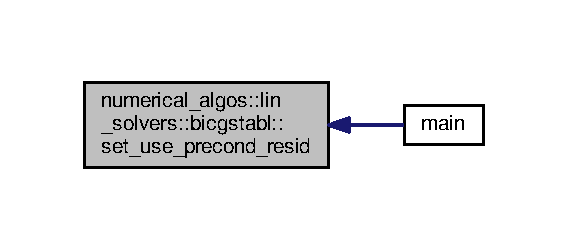
\includegraphics[width=272pt]{classnumerical__algos_1_1lin__solvers_1_1bicgstabl_ab420850c21b5e6a86cd41491e309cb56_icgraph}
\end{center}
\end{figure}


\hypertarget{classnumerical__algos_1_1lin__solvers_1_1bicgstabl_a384c0d158f1f920be404a0165672965f}{\index{numerical\-\_\-algos\-::lin\-\_\-solvers\-::bicgstabl@{numerical\-\_\-algos\-::lin\-\_\-solvers\-::bicgstabl}!set\-\_\-use\-\_\-real\-\_\-resid@{set\-\_\-use\-\_\-real\-\_\-resid}}
\index{set\-\_\-use\-\_\-real\-\_\-resid@{set\-\_\-use\-\_\-real\-\_\-resid}!numerical_algos::lin_solvers::bicgstabl@{numerical\-\_\-algos\-::lin\-\_\-solvers\-::bicgstabl}}
\subsubsection[{set\-\_\-use\-\_\-real\-\_\-resid}]{\setlength{\rightskip}{0pt plus 5cm}template$<$class Linear\-Operator , class Preconditioner , class Vector\-Operations , class Monitor , class Log $>$ void {\bf numerical\-\_\-algos\-::lin\-\_\-solvers\-::bicgstabl}$<$ Linear\-Operator, Preconditioner, Vector\-Operations, Monitor, Log $>$\-::set\-\_\-use\-\_\-real\-\_\-resid (
\begin{DoxyParamCaption}
\item[{bool}]{use\-\_\-real\-\_\-resid}
\end{DoxyParamCaption}
)\hspace{0.3cm}{\ttfamily [inline]}}}\label{classnumerical__algos_1_1lin__solvers_1_1bicgstabl_a384c0d158f1f920be404a0165672965f}


Here is the caller graph for this function\-:
\nopagebreak
\begin{figure}[H]
\begin{center}
\leavevmode
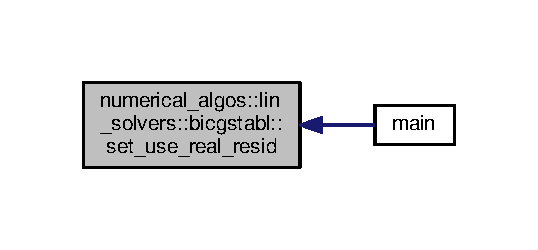
\includegraphics[width=258pt]{classnumerical__algos_1_1lin__solvers_1_1bicgstabl_a384c0d158f1f920be404a0165672965f_icgraph}
\end{center}
\end{figure}


\hypertarget{classnumerical__algos_1_1lin__solvers_1_1bicgstabl_a2dd4f6cdd207b1a77aa94831fbdf9839}{\index{numerical\-\_\-algos\-::lin\-\_\-solvers\-::bicgstabl@{numerical\-\_\-algos\-::lin\-\_\-solvers\-::bicgstabl}!solve@{solve}}
\index{solve@{solve}!numerical_algos::lin_solvers::bicgstabl@{numerical\-\_\-algos\-::lin\-\_\-solvers\-::bicgstabl}}
\subsubsection[{solve}]{\setlength{\rightskip}{0pt plus 5cm}template$<$class Linear\-Operator , class Preconditioner , class Vector\-Operations , class Monitor , class Log $>$ virtual bool {\bf numerical\-\_\-algos\-::lin\-\_\-solvers\-::bicgstabl}$<$ Linear\-Operator, Preconditioner, Vector\-Operations, Monitor, Log $>$\-::solve (
\begin{DoxyParamCaption}
\item[{const {\bf linear\-\_\-operator\-\_\-type} \&}]{A, }
\item[{const {\bf vector\-\_\-type} \&}]{b, }
\item[{{\bf vector\-\_\-type} \&}]{x}
\end{DoxyParamCaption}
) const\hspace{0.3cm}{\ttfamily [inline]}, {\ttfamily [virtual]}}}\label{classnumerical__algos_1_1lin__solvers_1_1bicgstabl_a2dd4f6cdd207b1a77aa94831fbdf9839}


Implements \hyperlink{classnumerical__algos_1_1lin__solvers_1_1iter__solver__base_ac21be1f601f4937a97c0d3df3182a2af}{numerical\-\_\-algos\-::lin\-\_\-solvers\-::iter\-\_\-solver\-\_\-base$<$ Linear\-Operator, Preconditioner, Vector\-Operations, Monitor, Log $>$}.



Here is the call graph for this function\-:
\nopagebreak
\begin{figure}[H]
\begin{center}
\leavevmode
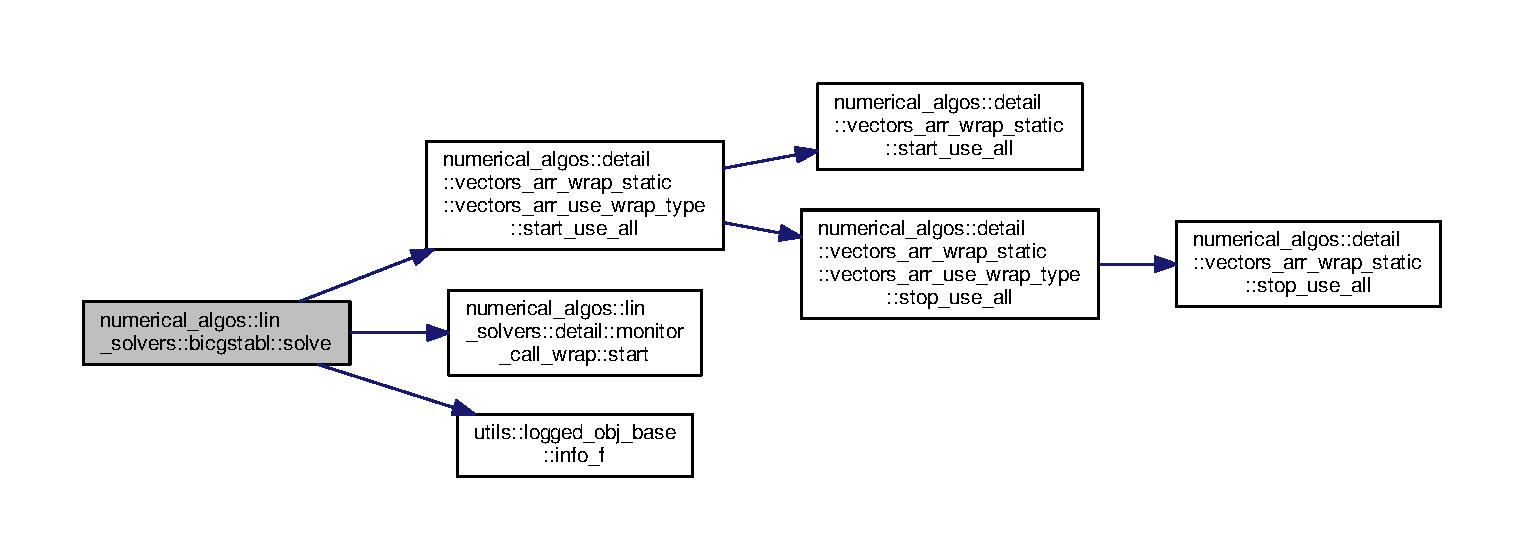
\includegraphics[width=350pt]{classnumerical__algos_1_1lin__solvers_1_1bicgstabl_a2dd4f6cdd207b1a77aa94831fbdf9839_cgraph}
\end{center}
\end{figure}


\hypertarget{classnumerical__algos_1_1lin__solvers_1_1bicgstabl_a2dd4f6cdd207b1a77aa94831fbdf9839}{\index{numerical\-\_\-algos\-::lin\-\_\-solvers\-::bicgstabl@{numerical\-\_\-algos\-::lin\-\_\-solvers\-::bicgstabl}!solve@{solve}}
\index{solve@{solve}!numerical_algos::lin_solvers::bicgstabl@{numerical\-\_\-algos\-::lin\-\_\-solvers\-::bicgstabl}}
\subsubsection[{solve}]{\setlength{\rightskip}{0pt plus 5cm}template$<$class Linear\-Operator , class Preconditioner , class Vector\-Operations , class Monitor , class Log $>$ virtual bool {\bf numerical\-\_\-algos\-::lin\-\_\-solvers\-::bicgstabl}$<$ Linear\-Operator, Preconditioner, Vector\-Operations, Monitor, Log $>$\-::solve (
\begin{DoxyParamCaption}
\item[{const {\bf linear\-\_\-operator\-\_\-type} \&}]{A, }
\item[{const {\bf vector\-\_\-type} \&}]{b, }
\item[{{\bf vector\-\_\-type} \&}]{x}
\end{DoxyParamCaption}
) const\hspace{0.3cm}{\ttfamily [inline]}, {\ttfamily [virtual]}}}\label{classnumerical__algos_1_1lin__solvers_1_1bicgstabl_a2dd4f6cdd207b1a77aa94831fbdf9839}


Implements \hyperlink{classnumerical__algos_1_1lin__solvers_1_1iter__solver__base_ac21be1f601f4937a97c0d3df3182a2af}{numerical\-\_\-algos\-::lin\-\_\-solvers\-::iter\-\_\-solver\-\_\-base$<$ Linear\-Operator, Preconditioner, Vector\-Operations, Monitor, Log $>$}.



Here is the call graph for this function\-:
\nopagebreak
\begin{figure}[H]
\begin{center}
\leavevmode
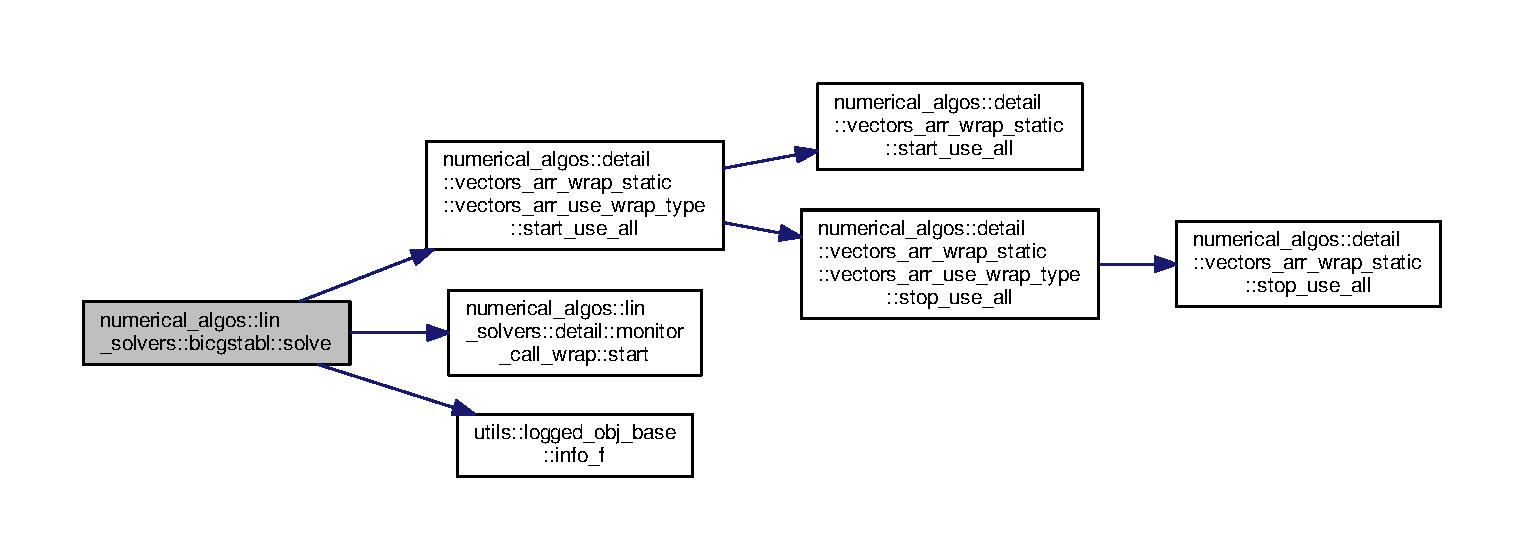
\includegraphics[width=350pt]{classnumerical__algos_1_1lin__solvers_1_1bicgstabl_a2dd4f6cdd207b1a77aa94831fbdf9839_cgraph}
\end{center}
\end{figure}




Here is the caller graph for this function\-:
\nopagebreak
\begin{figure}[H]
\begin{center}
\leavevmode
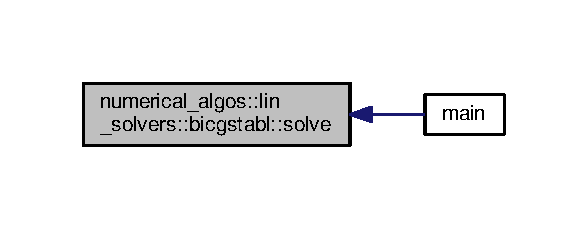
\includegraphics[width=282pt]{classnumerical__algos_1_1lin__solvers_1_1bicgstabl_a2dd4f6cdd207b1a77aa94831fbdf9839_icgraph}
\end{center}
\end{figure}




The documentation for this class was generated from the following files\-:\begin{DoxyCompactItemize}
\item 
source/numerical\-\_\-algos/lin\-\_\-solvers/\hyperlink{bicgstabl_8h}{bicgstabl.\-h}\item 
source/numerical\-\_\-algos/lin\-\_\-solvers/\hyperlink{bicgstabl__real__resid_8h}{bicgstabl\-\_\-real\-\_\-resid.\-h}\end{DoxyCompactItemize}

\hypertarget{classnumerical__algos_1_1lin__solvers_1_1cgs}{\section{numerical\-\_\-algos\-:\-:lin\-\_\-solvers\-:\-:cgs$<$ Linear\-Operator, Preconditioner, Vector\-Operations, Monitor, Log $>$ Class Template Reference}
\label{classnumerical__algos_1_1lin__solvers_1_1cgs}\index{numerical\-\_\-algos\-::lin\-\_\-solvers\-::cgs$<$ Linear\-Operator, Preconditioner, Vector\-Operations, Monitor, Log $>$@{numerical\-\_\-algos\-::lin\-\_\-solvers\-::cgs$<$ Linear\-Operator, Preconditioner, Vector\-Operations, Monitor, Log $>$}}
}


{\ttfamily \#include $<$cgs.\-h$>$}



Inheritance diagram for numerical\-\_\-algos\-:\-:lin\-\_\-solvers\-:\-:cgs$<$ Linear\-Operator, Preconditioner, Vector\-Operations, Monitor, Log $>$\-:\nopagebreak
\begin{figure}[H]
\begin{center}
\leavevmode
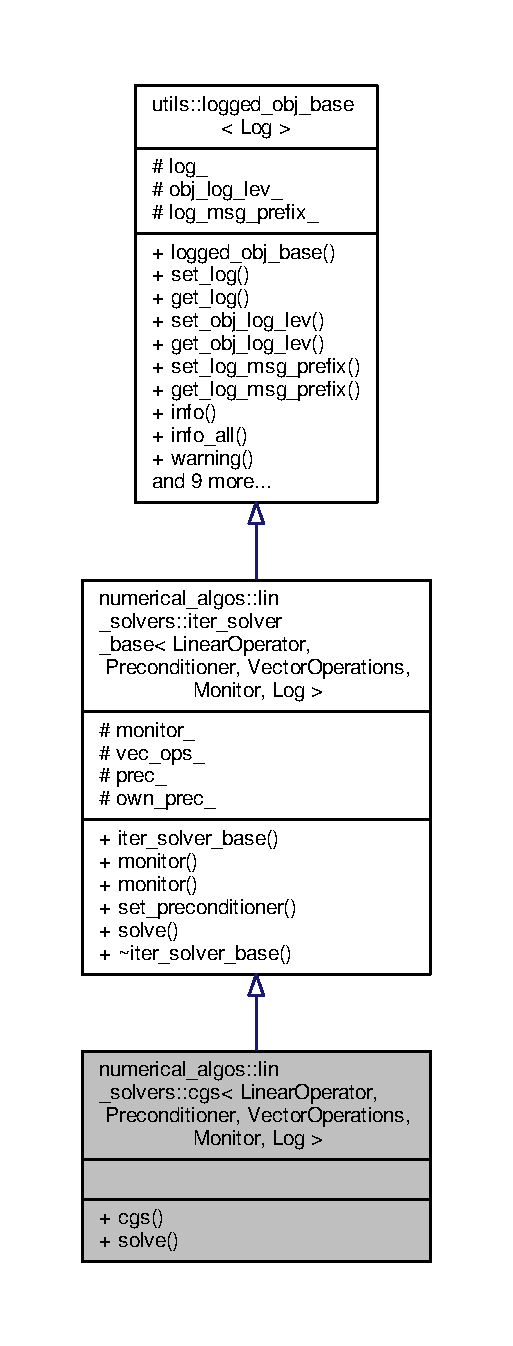
\includegraphics[height=550pt]{classnumerical__algos_1_1lin__solvers_1_1cgs__inherit__graph}
\end{center}
\end{figure}


Collaboration diagram for numerical\-\_\-algos\-:\-:lin\-\_\-solvers\-:\-:cgs$<$ Linear\-Operator, Preconditioner, Vector\-Operations, Monitor, Log $>$\-:\nopagebreak
\begin{figure}[H]
\begin{center}
\leavevmode
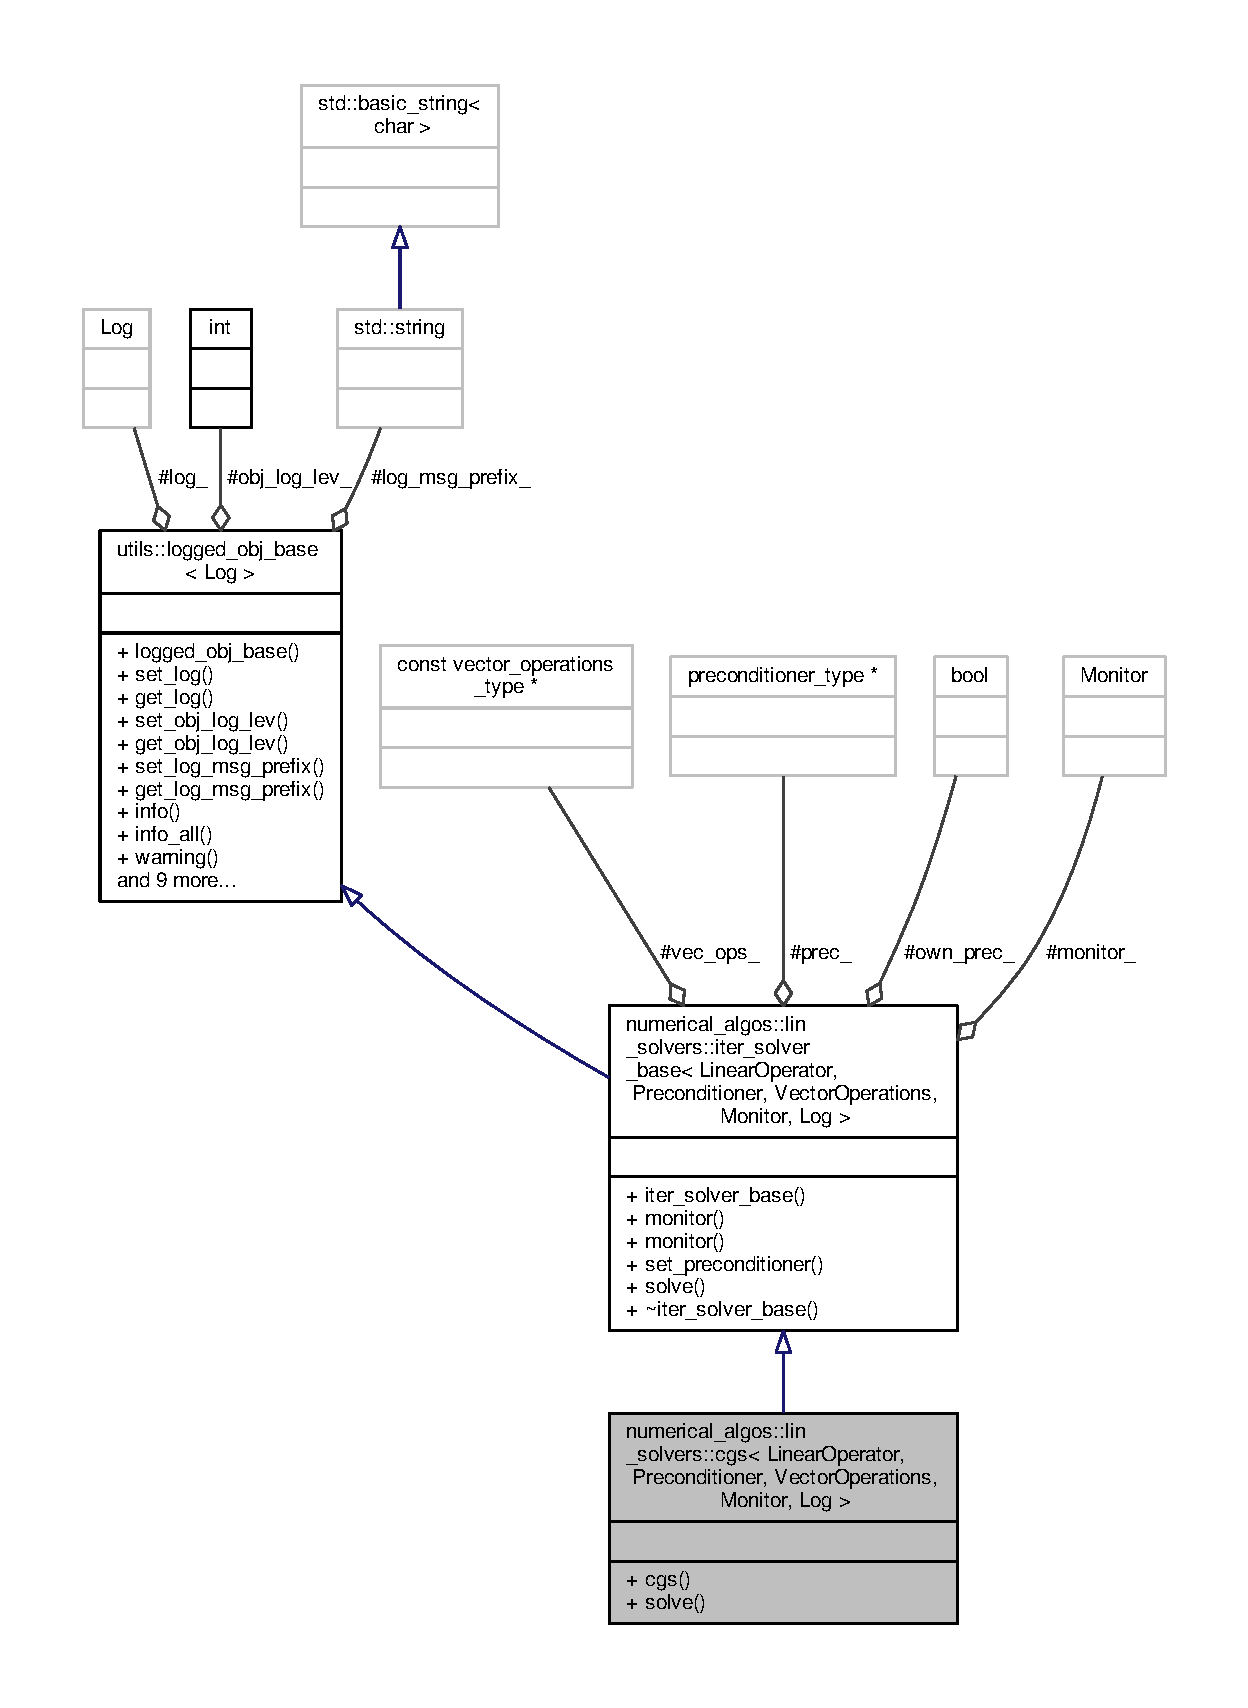
\includegraphics[width=350pt]{classnumerical__algos_1_1lin__solvers_1_1cgs__coll__graph}
\end{center}
\end{figure}
\subsection*{Public Types}
\begin{DoxyCompactItemize}
\item 
typedef \\*
Vector\-Operations\-::scalar\-\_\-type \hyperlink{classnumerical__algos_1_1lin__solvers_1_1cgs_a11a8155d321473c5940d28c23808154d}{scalar\-\_\-type}
\item 
typedef \\*
Vector\-Operations\-::vector\-\_\-type \hyperlink{classnumerical__algos_1_1lin__solvers_1_1cgs_aed6c8f0092b08fb3d0690c215cced5f9}{vector\-\_\-type}
\item 
typedef Linear\-Operator \hyperlink{classnumerical__algos_1_1lin__solvers_1_1cgs_a9aa9a945e8f133f9ef15f83a7a7880dc}{linear\-\_\-operator\-\_\-type}
\item 
typedef Preconditioner \hyperlink{classnumerical__algos_1_1lin__solvers_1_1cgs_ade373d56aec3d0a0c6414f773ca4f97f}{preconditioner\-\_\-type}
\item 
typedef Vector\-Operations \hyperlink{classnumerical__algos_1_1lin__solvers_1_1cgs_a249281fa342a90567f6344a57191fde9}{vector\-\_\-operations\-\_\-type}
\item 
typedef Monitor \hyperlink{classnumerical__algos_1_1lin__solvers_1_1cgs_af176eeddd3d6fc34241c1796ba381cf1}{monitor\-\_\-type}
\item 
typedef Log \hyperlink{classnumerical__algos_1_1lin__solvers_1_1cgs_af876166d874a6f33d2d626817605618f}{log\-\_\-type}
\end{DoxyCompactItemize}
\subsection*{Public Member Functions}
\begin{DoxyCompactItemize}
\item 
\hyperlink{classnumerical__algos_1_1lin__solvers_1_1cgs_af4672270c1d567b1d037e5b8c43f9944}{cgs} (const \hyperlink{classnumerical__algos_1_1lin__solvers_1_1cgs_a249281fa342a90567f6344a57191fde9}{vector\-\_\-operations\-\_\-type} $\ast$vec\-\_\-ops, Log $\ast$log=N\-U\-L\-L, \hyperlink{classint}{int} obj\-\_\-log\-\_\-lev=0)
\item 
virtual bool \hyperlink{classnumerical__algos_1_1lin__solvers_1_1cgs_a76503cf7b66739a4fa4571f034aa960e}{solve} (const \hyperlink{classnumerical__algos_1_1lin__solvers_1_1cgs_a9aa9a945e8f133f9ef15f83a7a7880dc}{linear\-\_\-operator\-\_\-type} \&A, const \hyperlink{classnumerical__algos_1_1lin__solvers_1_1cgs_aed6c8f0092b08fb3d0690c215cced5f9}{vector\-\_\-type} \&b, \hyperlink{classnumerical__algos_1_1lin__solvers_1_1cgs_aed6c8f0092b08fb3d0690c215cced5f9}{vector\-\_\-type} \&x) const 
\end{DoxyCompactItemize}
\subsection*{Additional Inherited Members}


\subsection{Member Typedef Documentation}
\hypertarget{classnumerical__algos_1_1lin__solvers_1_1cgs_a9aa9a945e8f133f9ef15f83a7a7880dc}{\index{numerical\-\_\-algos\-::lin\-\_\-solvers\-::cgs@{numerical\-\_\-algos\-::lin\-\_\-solvers\-::cgs}!linear\-\_\-operator\-\_\-type@{linear\-\_\-operator\-\_\-type}}
\index{linear\-\_\-operator\-\_\-type@{linear\-\_\-operator\-\_\-type}!numerical_algos::lin_solvers::cgs@{numerical\-\_\-algos\-::lin\-\_\-solvers\-::cgs}}
\subsubsection[{linear\-\_\-operator\-\_\-type}]{\setlength{\rightskip}{0pt plus 5cm}template$<$class Linear\-Operator , class Preconditioner , class Vector\-Operations , class Monitor , class Log $>$ typedef Linear\-Operator {\bf numerical\-\_\-algos\-::lin\-\_\-solvers\-::cgs}$<$ Linear\-Operator, Preconditioner, Vector\-Operations, Monitor, Log $>$\-::{\bf linear\-\_\-operator\-\_\-type}}}\label{classnumerical__algos_1_1lin__solvers_1_1cgs_a9aa9a945e8f133f9ef15f83a7a7880dc}
\hypertarget{classnumerical__algos_1_1lin__solvers_1_1cgs_af876166d874a6f33d2d626817605618f}{\index{numerical\-\_\-algos\-::lin\-\_\-solvers\-::cgs@{numerical\-\_\-algos\-::lin\-\_\-solvers\-::cgs}!log\-\_\-type@{log\-\_\-type}}
\index{log\-\_\-type@{log\-\_\-type}!numerical_algos::lin_solvers::cgs@{numerical\-\_\-algos\-::lin\-\_\-solvers\-::cgs}}
\subsubsection[{log\-\_\-type}]{\setlength{\rightskip}{0pt plus 5cm}template$<$class Linear\-Operator , class Preconditioner , class Vector\-Operations , class Monitor , class Log $>$ typedef Log {\bf numerical\-\_\-algos\-::lin\-\_\-solvers\-::cgs}$<$ Linear\-Operator, Preconditioner, Vector\-Operations, Monitor, Log $>$\-::{\bf log\-\_\-type}}}\label{classnumerical__algos_1_1lin__solvers_1_1cgs_af876166d874a6f33d2d626817605618f}
\hypertarget{classnumerical__algos_1_1lin__solvers_1_1cgs_af176eeddd3d6fc34241c1796ba381cf1}{\index{numerical\-\_\-algos\-::lin\-\_\-solvers\-::cgs@{numerical\-\_\-algos\-::lin\-\_\-solvers\-::cgs}!monitor\-\_\-type@{monitor\-\_\-type}}
\index{monitor\-\_\-type@{monitor\-\_\-type}!numerical_algos::lin_solvers::cgs@{numerical\-\_\-algos\-::lin\-\_\-solvers\-::cgs}}
\subsubsection[{monitor\-\_\-type}]{\setlength{\rightskip}{0pt plus 5cm}template$<$class Linear\-Operator , class Preconditioner , class Vector\-Operations , class Monitor , class Log $>$ typedef Monitor {\bf numerical\-\_\-algos\-::lin\-\_\-solvers\-::cgs}$<$ Linear\-Operator, Preconditioner, Vector\-Operations, Monitor, Log $>$\-::{\bf monitor\-\_\-type}}}\label{classnumerical__algos_1_1lin__solvers_1_1cgs_af176eeddd3d6fc34241c1796ba381cf1}
\hypertarget{classnumerical__algos_1_1lin__solvers_1_1cgs_ade373d56aec3d0a0c6414f773ca4f97f}{\index{numerical\-\_\-algos\-::lin\-\_\-solvers\-::cgs@{numerical\-\_\-algos\-::lin\-\_\-solvers\-::cgs}!preconditioner\-\_\-type@{preconditioner\-\_\-type}}
\index{preconditioner\-\_\-type@{preconditioner\-\_\-type}!numerical_algos::lin_solvers::cgs@{numerical\-\_\-algos\-::lin\-\_\-solvers\-::cgs}}
\subsubsection[{preconditioner\-\_\-type}]{\setlength{\rightskip}{0pt plus 5cm}template$<$class Linear\-Operator , class Preconditioner , class Vector\-Operations , class Monitor , class Log $>$ typedef Preconditioner {\bf numerical\-\_\-algos\-::lin\-\_\-solvers\-::cgs}$<$ Linear\-Operator, Preconditioner, Vector\-Operations, Monitor, Log $>$\-::{\bf preconditioner\-\_\-type}}}\label{classnumerical__algos_1_1lin__solvers_1_1cgs_ade373d56aec3d0a0c6414f773ca4f97f}
\hypertarget{classnumerical__algos_1_1lin__solvers_1_1cgs_a11a8155d321473c5940d28c23808154d}{\index{numerical\-\_\-algos\-::lin\-\_\-solvers\-::cgs@{numerical\-\_\-algos\-::lin\-\_\-solvers\-::cgs}!scalar\-\_\-type@{scalar\-\_\-type}}
\index{scalar\-\_\-type@{scalar\-\_\-type}!numerical_algos::lin_solvers::cgs@{numerical\-\_\-algos\-::lin\-\_\-solvers\-::cgs}}
\subsubsection[{scalar\-\_\-type}]{\setlength{\rightskip}{0pt plus 5cm}template$<$class Linear\-Operator , class Preconditioner , class Vector\-Operations , class Monitor , class Log $>$ typedef Vector\-Operations\-::scalar\-\_\-type {\bf numerical\-\_\-algos\-::lin\-\_\-solvers\-::cgs}$<$ Linear\-Operator, Preconditioner, Vector\-Operations, Monitor, Log $>$\-::{\bf scalar\-\_\-type}}}\label{classnumerical__algos_1_1lin__solvers_1_1cgs_a11a8155d321473c5940d28c23808154d}
\hypertarget{classnumerical__algos_1_1lin__solvers_1_1cgs_a249281fa342a90567f6344a57191fde9}{\index{numerical\-\_\-algos\-::lin\-\_\-solvers\-::cgs@{numerical\-\_\-algos\-::lin\-\_\-solvers\-::cgs}!vector\-\_\-operations\-\_\-type@{vector\-\_\-operations\-\_\-type}}
\index{vector\-\_\-operations\-\_\-type@{vector\-\_\-operations\-\_\-type}!numerical_algos::lin_solvers::cgs@{numerical\-\_\-algos\-::lin\-\_\-solvers\-::cgs}}
\subsubsection[{vector\-\_\-operations\-\_\-type}]{\setlength{\rightskip}{0pt plus 5cm}template$<$class Linear\-Operator , class Preconditioner , class Vector\-Operations , class Monitor , class Log $>$ typedef Vector\-Operations {\bf numerical\-\_\-algos\-::lin\-\_\-solvers\-::cgs}$<$ Linear\-Operator, Preconditioner, Vector\-Operations, Monitor, Log $>$\-::{\bf vector\-\_\-operations\-\_\-type}}}\label{classnumerical__algos_1_1lin__solvers_1_1cgs_a249281fa342a90567f6344a57191fde9}
\hypertarget{classnumerical__algos_1_1lin__solvers_1_1cgs_aed6c8f0092b08fb3d0690c215cced5f9}{\index{numerical\-\_\-algos\-::lin\-\_\-solvers\-::cgs@{numerical\-\_\-algos\-::lin\-\_\-solvers\-::cgs}!vector\-\_\-type@{vector\-\_\-type}}
\index{vector\-\_\-type@{vector\-\_\-type}!numerical_algos::lin_solvers::cgs@{numerical\-\_\-algos\-::lin\-\_\-solvers\-::cgs}}
\subsubsection[{vector\-\_\-type}]{\setlength{\rightskip}{0pt plus 5cm}template$<$class Linear\-Operator , class Preconditioner , class Vector\-Operations , class Monitor , class Log $>$ typedef Vector\-Operations\-::vector\-\_\-type {\bf numerical\-\_\-algos\-::lin\-\_\-solvers\-::cgs}$<$ Linear\-Operator, Preconditioner, Vector\-Operations, Monitor, Log $>$\-::{\bf vector\-\_\-type}}}\label{classnumerical__algos_1_1lin__solvers_1_1cgs_aed6c8f0092b08fb3d0690c215cced5f9}


\subsection{Constructor \& Destructor Documentation}
\hypertarget{classnumerical__algos_1_1lin__solvers_1_1cgs_af4672270c1d567b1d037e5b8c43f9944}{\index{numerical\-\_\-algos\-::lin\-\_\-solvers\-::cgs@{numerical\-\_\-algos\-::lin\-\_\-solvers\-::cgs}!cgs@{cgs}}
\index{cgs@{cgs}!numerical_algos::lin_solvers::cgs@{numerical\-\_\-algos\-::lin\-\_\-solvers\-::cgs}}
\subsubsection[{cgs}]{\setlength{\rightskip}{0pt plus 5cm}template$<$class Linear\-Operator , class Preconditioner , class Vector\-Operations , class Monitor , class Log $>$ {\bf numerical\-\_\-algos\-::lin\-\_\-solvers\-::cgs}$<$ Linear\-Operator, Preconditioner, Vector\-Operations, Monitor, Log $>$\-::{\bf cgs} (
\begin{DoxyParamCaption}
\item[{const {\bf vector\-\_\-operations\-\_\-type} $\ast$}]{vec\-\_\-ops, }
\item[{Log $\ast$}]{log = {\ttfamily NULL}, }
\item[{{\bf int}}]{obj\-\_\-log\-\_\-lev = {\ttfamily 0}}
\end{DoxyParamCaption}
)\hspace{0.3cm}{\ttfamily [inline]}}}\label{classnumerical__algos_1_1lin__solvers_1_1cgs_af4672270c1d567b1d037e5b8c43f9944}


Here is the call graph for this function\-:\nopagebreak
\begin{figure}[H]
\begin{center}
\leavevmode
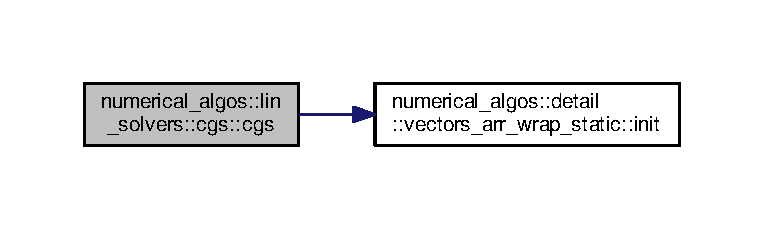
\includegraphics[width=350pt]{classnumerical__algos_1_1lin__solvers_1_1cgs_af4672270c1d567b1d037e5b8c43f9944_cgraph}
\end{center}
\end{figure}




\subsection{Member Function Documentation}
\hypertarget{classnumerical__algos_1_1lin__solvers_1_1cgs_a76503cf7b66739a4fa4571f034aa960e}{\index{numerical\-\_\-algos\-::lin\-\_\-solvers\-::cgs@{numerical\-\_\-algos\-::lin\-\_\-solvers\-::cgs}!solve@{solve}}
\index{solve@{solve}!numerical_algos::lin_solvers::cgs@{numerical\-\_\-algos\-::lin\-\_\-solvers\-::cgs}}
\subsubsection[{solve}]{\setlength{\rightskip}{0pt plus 5cm}template$<$class Linear\-Operator , class Preconditioner , class Vector\-Operations , class Monitor , class Log $>$ virtual bool {\bf numerical\-\_\-algos\-::lin\-\_\-solvers\-::cgs}$<$ Linear\-Operator, Preconditioner, Vector\-Operations, Monitor, Log $>$\-::solve (
\begin{DoxyParamCaption}
\item[{const {\bf linear\-\_\-operator\-\_\-type} \&}]{A, }
\item[{const {\bf vector\-\_\-type} \&}]{b, }
\item[{{\bf vector\-\_\-type} \&}]{x}
\end{DoxyParamCaption}
) const\hspace{0.3cm}{\ttfamily [inline]}, {\ttfamily [virtual]}}}\label{classnumerical__algos_1_1lin__solvers_1_1cgs_a76503cf7b66739a4fa4571f034aa960e}


Implements \hyperlink{classnumerical__algos_1_1lin__solvers_1_1iter__solver__base_ac21be1f601f4937a97c0d3df3182a2af}{numerical\-\_\-algos\-::lin\-\_\-solvers\-::iter\-\_\-solver\-\_\-base$<$ Linear\-Operator, Preconditioner, Vector\-Operations, Monitor, Log $>$}.



Here is the call graph for this function\-:\nopagebreak
\begin{figure}[H]
\begin{center}
\leavevmode
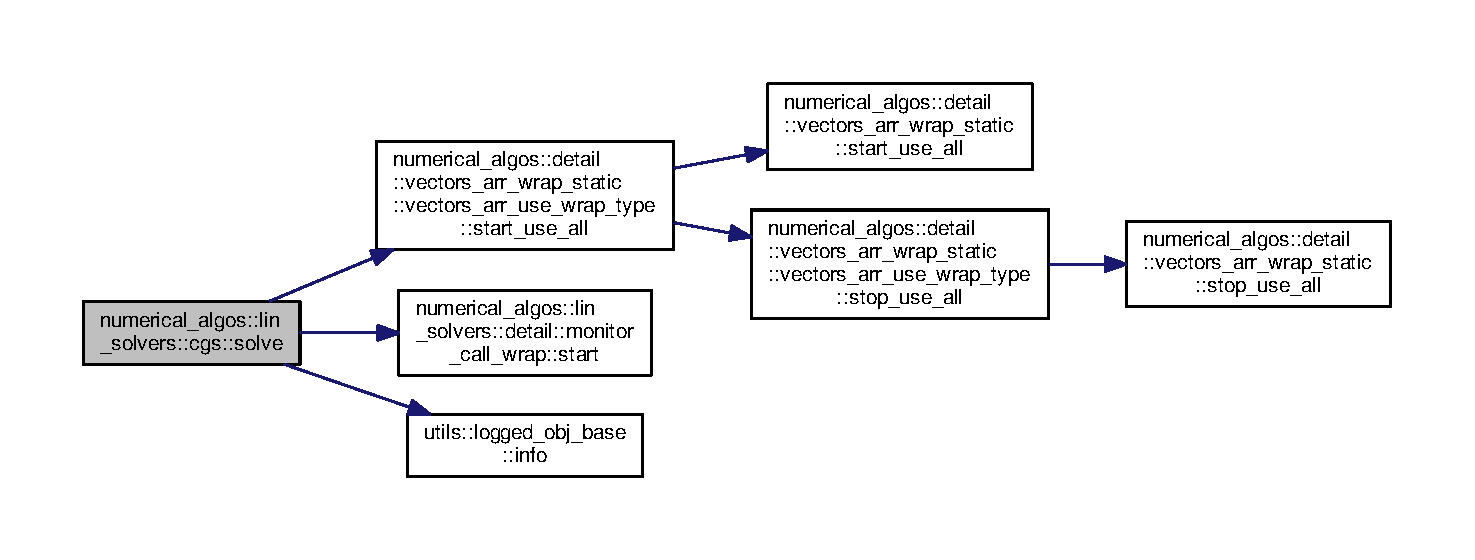
\includegraphics[width=350pt]{classnumerical__algos_1_1lin__solvers_1_1cgs_a76503cf7b66739a4fa4571f034aa960e_cgraph}
\end{center}
\end{figure}




Here is the caller graph for this function\-:\nopagebreak
\begin{figure}[H]
\begin{center}
\leavevmode
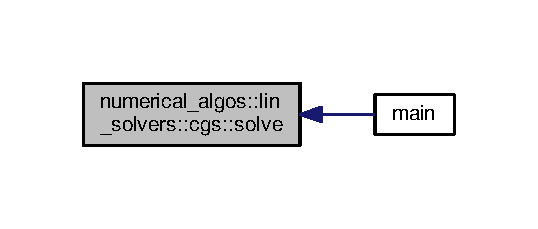
\includegraphics[width=258pt]{classnumerical__algos_1_1lin__solvers_1_1cgs_a76503cf7b66739a4fa4571f034aa960e_icgraph}
\end{center}
\end{figure}




The documentation for this class was generated from the following file\-:\begin{DoxyCompactItemize}
\item 
source/numerical\-\_\-algos/lin\-\_\-solvers/\hyperlink{cgs_8h}{cgs.\-h}\end{DoxyCompactItemize}

\hypertarget{classtest__class_1_1class__file}{\section{test\-\_\-class\-:\-:class\-\_\-file$<$ T, B\-L\-O\-C\-K\-\_\-\-S\-I\-Z\-E $>$ Class Template Reference}
\label{classtest__class_1_1class__file}\index{test\-\_\-class\-::class\-\_\-file$<$ T, B\-L\-O\-C\-K\-\_\-\-S\-I\-Z\-E $>$@{test\-\_\-class\-::class\-\_\-file$<$ T, B\-L\-O\-C\-K\-\_\-\-S\-I\-Z\-E $>$}}
}


{\ttfamily \#include $<$class\-\_\-file.\-h$>$}



Collaboration diagram for test\-\_\-class\-:\-:class\-\_\-file$<$ T, B\-L\-O\-C\-K\-\_\-\-S\-I\-Z\-E $>$\-:
\nopagebreak
\begin{figure}[H]
\begin{center}
\leavevmode
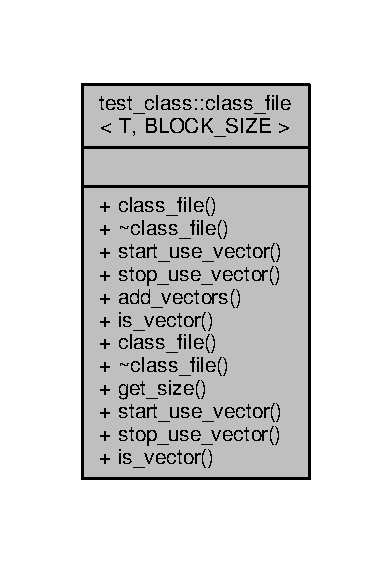
\includegraphics[width=188pt]{classtest__class_1_1class__file__coll__graph}
\end{center}
\end{figure}
\subsection*{Classes}
\begin{DoxyCompactItemize}
\item 
class \hyperlink{classtest__class_1_1class__file_1_1nested__class}{nested\-\_\-class}
\end{DoxyCompactItemize}
\subsection*{Public Types}
\begin{DoxyCompactItemize}
\item 
typedef T \hyperlink{classtest__class_1_1class__file_a4a1b0b0803393eef737a5af7de611879}{scalar\-\_\-type}
\item 
typedef T $\ast$ \hyperlink{classtest__class_1_1class__file_abe63b9f832b951bdde090c87f78a92a5}{vector\-\_\-type}
\item 
typedef T \hyperlink{classtest__class_1_1class__file_a4a1b0b0803393eef737a5af7de611879}{scalar\-\_\-type}
\item 
typedef T $\ast$ \hyperlink{classtest__class_1_1class__file_abe63b9f832b951bdde090c87f78a92a5}{vector\-\_\-type}
\end{DoxyCompactItemize}
\subsection*{Public Member Functions}
\begin{DoxyCompactItemize}
\item 
\hyperlink{classtest__class_1_1class__file_a892ae15bc27c844d0946bdaf02322aed}{class\-\_\-file} (size\-\_\-t sz\-\_\-)
\item 
\hyperlink{classtest__class_1_1class__file_af9024a9e3acf28dd5ac62c36a59fa48d}{$\sim$class\-\_\-file} ()
\item 
void \hyperlink{classtest__class_1_1class__file_ae0bbcb0c47c4332631581af9132a17c3}{start\-\_\-use\-\_\-vector} (T $\ast$\&x)
\item 
void \hyperlink{classtest__class_1_1class__file_a61c9997de3a72818b730b20812436e4f}{stop\-\_\-use\-\_\-vector} (T $\ast$\&x)
\item 
void \hyperlink{classtest__class_1_1class__file_aa92d0aaaa73a077fd8257ac4d2638a19}{add\-\_\-vectors} (const T $\ast$\&x, T $\ast$\&y)
\item 
bool \hyperlink{classtest__class_1_1class__file_a93c134c56388038d2ce68b5db3278044}{is\-\_\-vector} (const T $\ast$\&x) const 
\item 
\hyperlink{classtest__class_1_1class__file_a892ae15bc27c844d0946bdaf02322aed}{class\-\_\-file} (size\-\_\-t sz\-\_\-)
\item 
\hyperlink{classtest__class_1_1class__file_af9024a9e3acf28dd5ac62c36a59fa48d}{$\sim$class\-\_\-file} ()
\item 
size\-\_\-t \hyperlink{classtest__class_1_1class__file_a94a68418bcbcd7fd27dcf7832bd62f5b}{get\-\_\-size} ()
\item 
void \hyperlink{classtest__class_1_1class__file_ae0bbcb0c47c4332631581af9132a17c3}{start\-\_\-use\-\_\-vector} (T $\ast$\&x)
\item 
void \hyperlink{classtest__class_1_1class__file_a61c9997de3a72818b730b20812436e4f}{stop\-\_\-use\-\_\-vector} (T $\ast$\&x)
\item 
bool \hyperlink{classtest__class_1_1class__file_a93c134c56388038d2ce68b5db3278044}{is\-\_\-vector} (const T $\ast$\&x) const 
\end{DoxyCompactItemize}


\subsection{Member Typedef Documentation}
\hypertarget{classtest__class_1_1class__file_a4a1b0b0803393eef737a5af7de611879}{\index{test\-\_\-class\-::class\-\_\-file@{test\-\_\-class\-::class\-\_\-file}!scalar\-\_\-type@{scalar\-\_\-type}}
\index{scalar\-\_\-type@{scalar\-\_\-type}!test_class::class_file@{test\-\_\-class\-::class\-\_\-file}}
\subsubsection[{scalar\-\_\-type}]{\setlength{\rightskip}{0pt plus 5cm}template$<$typename T, int B\-L\-O\-C\-K\-\_\-\-S\-I\-Z\-E = 256$>$ typedef T {\bf test\-\_\-class\-::class\-\_\-file}$<$ T, B\-L\-O\-C\-K\-\_\-\-S\-I\-Z\-E $>$\-::{\bf scalar\-\_\-type}}}\label{classtest__class_1_1class__file_a4a1b0b0803393eef737a5af7de611879}
\hypertarget{classtest__class_1_1class__file_a4a1b0b0803393eef737a5af7de611879}{\index{test\-\_\-class\-::class\-\_\-file@{test\-\_\-class\-::class\-\_\-file}!scalar\-\_\-type@{scalar\-\_\-type}}
\index{scalar\-\_\-type@{scalar\-\_\-type}!test_class::class_file@{test\-\_\-class\-::class\-\_\-file}}
\subsubsection[{scalar\-\_\-type}]{\setlength{\rightskip}{0pt plus 5cm}template$<$typename T, int B\-L\-O\-C\-K\-\_\-\-S\-I\-Z\-E = 256$>$ typedef T {\bf test\-\_\-class\-::class\-\_\-file}$<$ T, B\-L\-O\-C\-K\-\_\-\-S\-I\-Z\-E $>$\-::{\bf scalar\-\_\-type}}}\label{classtest__class_1_1class__file_a4a1b0b0803393eef737a5af7de611879}
\hypertarget{classtest__class_1_1class__file_abe63b9f832b951bdde090c87f78a92a5}{\index{test\-\_\-class\-::class\-\_\-file@{test\-\_\-class\-::class\-\_\-file}!vector\-\_\-type@{vector\-\_\-type}}
\index{vector\-\_\-type@{vector\-\_\-type}!test_class::class_file@{test\-\_\-class\-::class\-\_\-file}}
\subsubsection[{vector\-\_\-type}]{\setlength{\rightskip}{0pt plus 5cm}template$<$typename T, int B\-L\-O\-C\-K\-\_\-\-S\-I\-Z\-E = 256$>$ typedef T$\ast$ {\bf test\-\_\-class\-::class\-\_\-file}$<$ T, B\-L\-O\-C\-K\-\_\-\-S\-I\-Z\-E $>$\-::{\bf vector\-\_\-type}}}\label{classtest__class_1_1class__file_abe63b9f832b951bdde090c87f78a92a5}
\hypertarget{classtest__class_1_1class__file_abe63b9f832b951bdde090c87f78a92a5}{\index{test\-\_\-class\-::class\-\_\-file@{test\-\_\-class\-::class\-\_\-file}!vector\-\_\-type@{vector\-\_\-type}}
\index{vector\-\_\-type@{vector\-\_\-type}!test_class::class_file@{test\-\_\-class\-::class\-\_\-file}}
\subsubsection[{vector\-\_\-type}]{\setlength{\rightskip}{0pt plus 5cm}template$<$typename T, int B\-L\-O\-C\-K\-\_\-\-S\-I\-Z\-E = 256$>$ typedef T$\ast$ {\bf test\-\_\-class\-::class\-\_\-file}$<$ T, B\-L\-O\-C\-K\-\_\-\-S\-I\-Z\-E $>$\-::{\bf vector\-\_\-type}}}\label{classtest__class_1_1class__file_abe63b9f832b951bdde090c87f78a92a5}


\subsection{Constructor \& Destructor Documentation}
\hypertarget{classtest__class_1_1class__file_a892ae15bc27c844d0946bdaf02322aed}{\index{test\-\_\-class\-::class\-\_\-file@{test\-\_\-class\-::class\-\_\-file}!class\-\_\-file@{class\-\_\-file}}
\index{class\-\_\-file@{class\-\_\-file}!test_class::class_file@{test\-\_\-class\-::class\-\_\-file}}
\subsubsection[{class\-\_\-file}]{\setlength{\rightskip}{0pt plus 5cm}template$<$typename T, int B\-L\-O\-C\-K\-\_\-\-S\-I\-Z\-E = 256$>$ {\bf test\-\_\-class\-::class\-\_\-file}$<$ T, B\-L\-O\-C\-K\-\_\-\-S\-I\-Z\-E $>$\-::{\bf class\-\_\-file} (
\begin{DoxyParamCaption}
\item[{size\-\_\-t}]{sz\-\_\-}
\end{DoxyParamCaption}
)\hspace{0.3cm}{\ttfamily [inline]}}}\label{classtest__class_1_1class__file_a892ae15bc27c844d0946bdaf02322aed}
\hypertarget{classtest__class_1_1class__file_af9024a9e3acf28dd5ac62c36a59fa48d}{\index{test\-\_\-class\-::class\-\_\-file@{test\-\_\-class\-::class\-\_\-file}!$\sim$class\-\_\-file@{$\sim$class\-\_\-file}}
\index{$\sim$class\-\_\-file@{$\sim$class\-\_\-file}!test_class::class_file@{test\-\_\-class\-::class\-\_\-file}}
\subsubsection[{$\sim$class\-\_\-file}]{\setlength{\rightskip}{0pt plus 5cm}template$<$typename T, int B\-L\-O\-C\-K\-\_\-\-S\-I\-Z\-E = 256$>$ {\bf test\-\_\-class\-::class\-\_\-file}$<$ T, B\-L\-O\-C\-K\-\_\-\-S\-I\-Z\-E $>$\-::$\sim${\bf class\-\_\-file} (
\begin{DoxyParamCaption}
{}
\end{DoxyParamCaption}
)\hspace{0.3cm}{\ttfamily [inline]}}}\label{classtest__class_1_1class__file_af9024a9e3acf28dd5ac62c36a59fa48d}
\hypertarget{classtest__class_1_1class__file_a892ae15bc27c844d0946bdaf02322aed}{\index{test\-\_\-class\-::class\-\_\-file@{test\-\_\-class\-::class\-\_\-file}!class\-\_\-file@{class\-\_\-file}}
\index{class\-\_\-file@{class\-\_\-file}!test_class::class_file@{test\-\_\-class\-::class\-\_\-file}}
\subsubsection[{class\-\_\-file}]{\setlength{\rightskip}{0pt plus 5cm}template$<$typename T, int B\-L\-O\-C\-K\-\_\-\-S\-I\-Z\-E = 256$>$ {\bf test\-\_\-class\-::class\-\_\-file}$<$ T, B\-L\-O\-C\-K\-\_\-\-S\-I\-Z\-E $>$\-::{\bf class\-\_\-file} (
\begin{DoxyParamCaption}
\item[{size\-\_\-t}]{sz\-\_\-}
\end{DoxyParamCaption}
)\hspace{0.3cm}{\ttfamily [inline]}}}\label{classtest__class_1_1class__file_a892ae15bc27c844d0946bdaf02322aed}
\hypertarget{classtest__class_1_1class__file_af9024a9e3acf28dd5ac62c36a59fa48d}{\index{test\-\_\-class\-::class\-\_\-file@{test\-\_\-class\-::class\-\_\-file}!$\sim$class\-\_\-file@{$\sim$class\-\_\-file}}
\index{$\sim$class\-\_\-file@{$\sim$class\-\_\-file}!test_class::class_file@{test\-\_\-class\-::class\-\_\-file}}
\subsubsection[{$\sim$class\-\_\-file}]{\setlength{\rightskip}{0pt plus 5cm}template$<$typename T, int B\-L\-O\-C\-K\-\_\-\-S\-I\-Z\-E = 256$>$ {\bf test\-\_\-class\-::class\-\_\-file}$<$ T, B\-L\-O\-C\-K\-\_\-\-S\-I\-Z\-E $>$\-::$\sim${\bf class\-\_\-file} (
\begin{DoxyParamCaption}
{}
\end{DoxyParamCaption}
)\hspace{0.3cm}{\ttfamily [inline]}}}\label{classtest__class_1_1class__file_af9024a9e3acf28dd5ac62c36a59fa48d}


\subsection{Member Function Documentation}
\hypertarget{classtest__class_1_1class__file_aa92d0aaaa73a077fd8257ac4d2638a19}{\index{test\-\_\-class\-::class\-\_\-file@{test\-\_\-class\-::class\-\_\-file}!add\-\_\-vectors@{add\-\_\-vectors}}
\index{add\-\_\-vectors@{add\-\_\-vectors}!test_class::class_file@{test\-\_\-class\-::class\-\_\-file}}
\subsubsection[{add\-\_\-vectors}]{\setlength{\rightskip}{0pt plus 5cm}template$<$typename T, int B\-L\-O\-C\-K\-\_\-\-S\-I\-Z\-E = 256$>$ void {\bf test\-\_\-class\-::class\-\_\-file}$<$ T, B\-L\-O\-C\-K\-\_\-\-S\-I\-Z\-E $>$\-::add\-\_\-vectors (
\begin{DoxyParamCaption}
\item[{const T $\ast$\&}]{x, }
\item[{T $\ast$\&}]{y}
\end{DoxyParamCaption}
)}}\label{classtest__class_1_1class__file_aa92d0aaaa73a077fd8257ac4d2638a19}


Here is the caller graph for this function\-:
\nopagebreak
\begin{figure}[H]
\begin{center}
\leavevmode
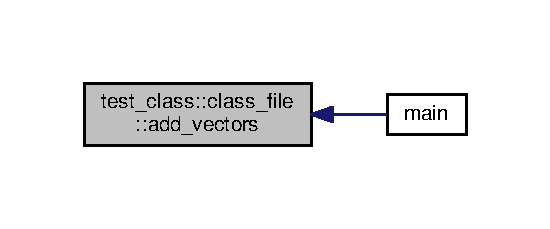
\includegraphics[width=264pt]{classtest__class_1_1class__file_aa92d0aaaa73a077fd8257ac4d2638a19_icgraph}
\end{center}
\end{figure}


\hypertarget{classtest__class_1_1class__file_a94a68418bcbcd7fd27dcf7832bd62f5b}{\index{test\-\_\-class\-::class\-\_\-file@{test\-\_\-class\-::class\-\_\-file}!get\-\_\-size@{get\-\_\-size}}
\index{get\-\_\-size@{get\-\_\-size}!test_class::class_file@{test\-\_\-class\-::class\-\_\-file}}
\subsubsection[{get\-\_\-size}]{\setlength{\rightskip}{0pt plus 5cm}template$<$typename T, int B\-L\-O\-C\-K\-\_\-\-S\-I\-Z\-E = 256$>$ size\-\_\-t {\bf test\-\_\-class\-::class\-\_\-file}$<$ T, B\-L\-O\-C\-K\-\_\-\-S\-I\-Z\-E $>$\-::get\-\_\-size (
\begin{DoxyParamCaption}
{}
\end{DoxyParamCaption}
)\hspace{0.3cm}{\ttfamily [inline]}}}\label{classtest__class_1_1class__file_a94a68418bcbcd7fd27dcf7832bd62f5b}
\hypertarget{classtest__class_1_1class__file_a93c134c56388038d2ce68b5db3278044}{\index{test\-\_\-class\-::class\-\_\-file@{test\-\_\-class\-::class\-\_\-file}!is\-\_\-vector@{is\-\_\-vector}}
\index{is\-\_\-vector@{is\-\_\-vector}!test_class::class_file@{test\-\_\-class\-::class\-\_\-file}}
\subsubsection[{is\-\_\-vector}]{\setlength{\rightskip}{0pt plus 5cm}template$<$typename T, int B\-L\-O\-C\-K\-\_\-\-S\-I\-Z\-E = 256$>$ bool {\bf test\-\_\-class\-::class\-\_\-file}$<$ T, B\-L\-O\-C\-K\-\_\-\-S\-I\-Z\-E $>$\-::is\-\_\-vector (
\begin{DoxyParamCaption}
\item[{const T $\ast$\&}]{x}
\end{DoxyParamCaption}
) const\hspace{0.3cm}{\ttfamily [inline]}}}\label{classtest__class_1_1class__file_a93c134c56388038d2ce68b5db3278044}
\hypertarget{classtest__class_1_1class__file_a93c134c56388038d2ce68b5db3278044}{\index{test\-\_\-class\-::class\-\_\-file@{test\-\_\-class\-::class\-\_\-file}!is\-\_\-vector@{is\-\_\-vector}}
\index{is\-\_\-vector@{is\-\_\-vector}!test_class::class_file@{test\-\_\-class\-::class\-\_\-file}}
\subsubsection[{is\-\_\-vector}]{\setlength{\rightskip}{0pt plus 5cm}template$<$typename T, int B\-L\-O\-C\-K\-\_\-\-S\-I\-Z\-E = 256$>$ bool {\bf test\-\_\-class\-::class\-\_\-file}$<$ T, B\-L\-O\-C\-K\-\_\-\-S\-I\-Z\-E $>$\-::is\-\_\-vector (
\begin{DoxyParamCaption}
\item[{const T $\ast$\&}]{x}
\end{DoxyParamCaption}
) const\hspace{0.3cm}{\ttfamily [inline]}}}\label{classtest__class_1_1class__file_a93c134c56388038d2ce68b5db3278044}
\hypertarget{classtest__class_1_1class__file_ae0bbcb0c47c4332631581af9132a17c3}{\index{test\-\_\-class\-::class\-\_\-file@{test\-\_\-class\-::class\-\_\-file}!start\-\_\-use\-\_\-vector@{start\-\_\-use\-\_\-vector}}
\index{start\-\_\-use\-\_\-vector@{start\-\_\-use\-\_\-vector}!test_class::class_file@{test\-\_\-class\-::class\-\_\-file}}
\subsubsection[{start\-\_\-use\-\_\-vector}]{\setlength{\rightskip}{0pt plus 5cm}template$<$typename T, int B\-L\-O\-C\-K\-\_\-\-S\-I\-Z\-E = 256$>$ void {\bf test\-\_\-class\-::class\-\_\-file}$<$ T, B\-L\-O\-C\-K\-\_\-\-S\-I\-Z\-E $>$\-::start\-\_\-use\-\_\-vector (
\begin{DoxyParamCaption}
\item[{T $\ast$\&}]{x}
\end{DoxyParamCaption}
)\hspace{0.3cm}{\ttfamily [inline]}}}\label{classtest__class_1_1class__file_ae0bbcb0c47c4332631581af9132a17c3}


Here is the caller graph for this function\-:
\nopagebreak
\begin{figure}[H]
\begin{center}
\leavevmode
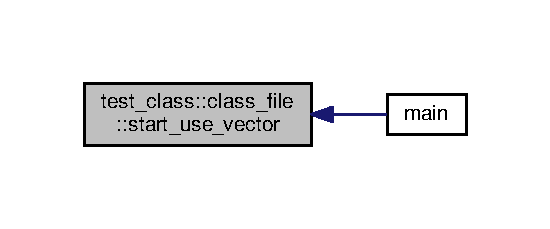
\includegraphics[width=264pt]{classtest__class_1_1class__file_ae0bbcb0c47c4332631581af9132a17c3_icgraph}
\end{center}
\end{figure}


\hypertarget{classtest__class_1_1class__file_ae0bbcb0c47c4332631581af9132a17c3}{\index{test\-\_\-class\-::class\-\_\-file@{test\-\_\-class\-::class\-\_\-file}!start\-\_\-use\-\_\-vector@{start\-\_\-use\-\_\-vector}}
\index{start\-\_\-use\-\_\-vector@{start\-\_\-use\-\_\-vector}!test_class::class_file@{test\-\_\-class\-::class\-\_\-file}}
\subsubsection[{start\-\_\-use\-\_\-vector}]{\setlength{\rightskip}{0pt plus 5cm}template$<$typename T, int B\-L\-O\-C\-K\-\_\-\-S\-I\-Z\-E = 256$>$ void {\bf test\-\_\-class\-::class\-\_\-file}$<$ T, B\-L\-O\-C\-K\-\_\-\-S\-I\-Z\-E $>$\-::start\-\_\-use\-\_\-vector (
\begin{DoxyParamCaption}
\item[{T $\ast$\&}]{x}
\end{DoxyParamCaption}
)\hspace{0.3cm}{\ttfamily [inline]}}}\label{classtest__class_1_1class__file_ae0bbcb0c47c4332631581af9132a17c3}


Here is the call graph for this function\-:
\nopagebreak
\begin{figure}[H]
\begin{center}
\leavevmode
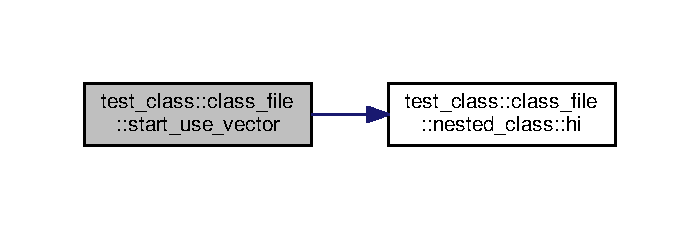
\includegraphics[width=336pt]{classtest__class_1_1class__file_ae0bbcb0c47c4332631581af9132a17c3_cgraph}
\end{center}
\end{figure}


\hypertarget{classtest__class_1_1class__file_a61c9997de3a72818b730b20812436e4f}{\index{test\-\_\-class\-::class\-\_\-file@{test\-\_\-class\-::class\-\_\-file}!stop\-\_\-use\-\_\-vector@{stop\-\_\-use\-\_\-vector}}
\index{stop\-\_\-use\-\_\-vector@{stop\-\_\-use\-\_\-vector}!test_class::class_file@{test\-\_\-class\-::class\-\_\-file}}
\subsubsection[{stop\-\_\-use\-\_\-vector}]{\setlength{\rightskip}{0pt plus 5cm}template$<$typename T, int B\-L\-O\-C\-K\-\_\-\-S\-I\-Z\-E = 256$>$ void {\bf test\-\_\-class\-::class\-\_\-file}$<$ T, B\-L\-O\-C\-K\-\_\-\-S\-I\-Z\-E $>$\-::stop\-\_\-use\-\_\-vector (
\begin{DoxyParamCaption}
\item[{T $\ast$\&}]{x}
\end{DoxyParamCaption}
)\hspace{0.3cm}{\ttfamily [inline]}}}\label{classtest__class_1_1class__file_a61c9997de3a72818b730b20812436e4f}


Here is the caller graph for this function\-:
\nopagebreak
\begin{figure}[H]
\begin{center}
\leavevmode
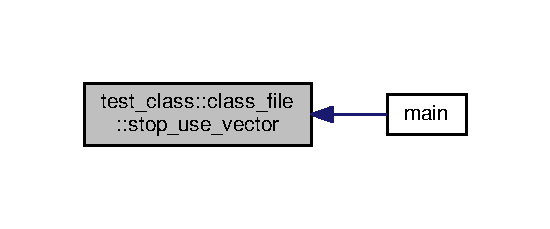
\includegraphics[width=264pt]{classtest__class_1_1class__file_a61c9997de3a72818b730b20812436e4f_icgraph}
\end{center}
\end{figure}


\hypertarget{classtest__class_1_1class__file_a61c9997de3a72818b730b20812436e4f}{\index{test\-\_\-class\-::class\-\_\-file@{test\-\_\-class\-::class\-\_\-file}!stop\-\_\-use\-\_\-vector@{stop\-\_\-use\-\_\-vector}}
\index{stop\-\_\-use\-\_\-vector@{stop\-\_\-use\-\_\-vector}!test_class::class_file@{test\-\_\-class\-::class\-\_\-file}}
\subsubsection[{stop\-\_\-use\-\_\-vector}]{\setlength{\rightskip}{0pt plus 5cm}template$<$typename T, int B\-L\-O\-C\-K\-\_\-\-S\-I\-Z\-E = 256$>$ void {\bf test\-\_\-class\-::class\-\_\-file}$<$ T, B\-L\-O\-C\-K\-\_\-\-S\-I\-Z\-E $>$\-::stop\-\_\-use\-\_\-vector (
\begin{DoxyParamCaption}
\item[{T $\ast$\&}]{x}
\end{DoxyParamCaption}
)\hspace{0.3cm}{\ttfamily [inline]}}}\label{classtest__class_1_1class__file_a61c9997de3a72818b730b20812436e4f}


The documentation for this class was generated from the following file\-:\begin{DoxyCompactItemize}
\item 
source/test\-\_\-inst/kernel\-\_\-class\-\_\-impl/\hyperlink{kernel__class__impl_2class__file_8h}{class\-\_\-file.\-h}\end{DoxyCompactItemize}

\hypertarget{classcomplex__div__test}{\section{complex\-\_\-div\-\_\-test$<$ vector\-\_\-operations\-\_\-\-R, vector\-\_\-operations\-\_\-\-C $>$ Class Template Reference}
\label{classcomplex__div__test}\index{complex\-\_\-div\-\_\-test$<$ vector\-\_\-operations\-\_\-\-R, vector\-\_\-operations\-\_\-\-C $>$@{complex\-\_\-div\-\_\-test$<$ vector\-\_\-operations\-\_\-\-R, vector\-\_\-operations\-\_\-\-C $>$}}
}


{\ttfamily \#include $<$complex\-\_\-div\-\_\-test.\-h$>$}



Collaboration diagram for complex\-\_\-div\-\_\-test$<$ vector\-\_\-operations\-\_\-\-R, vector\-\_\-operations\-\_\-\-C $>$\-:
\nopagebreak
\begin{figure}[H]
\begin{center}
\leavevmode
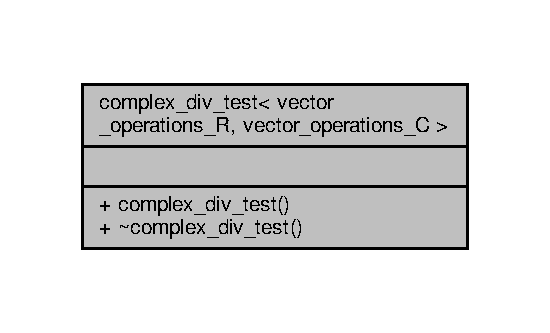
\includegraphics[width=264pt]{classcomplex__div__test__coll__graph}
\end{center}
\end{figure}
\subsection*{Public Member Functions}
\begin{DoxyCompactItemize}
\item 
\hyperlink{classcomplex__div__test_a3d35997bd401baeaaa5465d9b2501c04}{complex\-\_\-div\-\_\-test} ()
\item 
\hyperlink{classcomplex__div__test_a35749261def21774893118c1bdde22e8}{$\sim$complex\-\_\-div\-\_\-test} ()
\end{DoxyCompactItemize}


\subsection{Constructor \& Destructor Documentation}
\hypertarget{classcomplex__div__test_a3d35997bd401baeaaa5465d9b2501c04}{\index{complex\-\_\-div\-\_\-test@{complex\-\_\-div\-\_\-test}!complex\-\_\-div\-\_\-test@{complex\-\_\-div\-\_\-test}}
\index{complex\-\_\-div\-\_\-test@{complex\-\_\-div\-\_\-test}!complex_div_test@{complex\-\_\-div\-\_\-test}}
\subsubsection[{complex\-\_\-div\-\_\-test}]{\setlength{\rightskip}{0pt plus 5cm}template$<$class vector\-\_\-operations\-\_\-\-R , class vector\-\_\-operations\-\_\-\-C $>$ {\bf complex\-\_\-div\-\_\-test}$<$ vector\-\_\-operations\-\_\-\-R, vector\-\_\-operations\-\_\-\-C $>$\-::{\bf complex\-\_\-div\-\_\-test} (
\begin{DoxyParamCaption}
{}
\end{DoxyParamCaption}
)\hspace{0.3cm}{\ttfamily [inline]}}}\label{classcomplex__div__test_a3d35997bd401baeaaa5465d9b2501c04}
\hypertarget{classcomplex__div__test_a35749261def21774893118c1bdde22e8}{\index{complex\-\_\-div\-\_\-test@{complex\-\_\-div\-\_\-test}!$\sim$complex\-\_\-div\-\_\-test@{$\sim$complex\-\_\-div\-\_\-test}}
\index{$\sim$complex\-\_\-div\-\_\-test@{$\sim$complex\-\_\-div\-\_\-test}!complex_div_test@{complex\-\_\-div\-\_\-test}}
\subsubsection[{$\sim$complex\-\_\-div\-\_\-test}]{\setlength{\rightskip}{0pt plus 5cm}template$<$class vector\-\_\-operations\-\_\-\-R , class vector\-\_\-operations\-\_\-\-C $>$ {\bf complex\-\_\-div\-\_\-test}$<$ vector\-\_\-operations\-\_\-\-R, vector\-\_\-operations\-\_\-\-C $>$\-::$\sim${\bf complex\-\_\-div\-\_\-test} (
\begin{DoxyParamCaption}
{}
\end{DoxyParamCaption}
)\hspace{0.3cm}{\ttfamily [inline]}}}\label{classcomplex__div__test_a35749261def21774893118c1bdde22e8}


The documentation for this class was generated from the following file\-:\begin{DoxyCompactItemize}
\item 
source/test\-\_\-inst/complex\-\_\-div\-\_\-test/\hyperlink{complex__div__test_8h}{complex\-\_\-div\-\_\-test.\-h}\end{DoxyCompactItemize}

\hypertarget{structcomplex__type__hlp}{\section{complex\-\_\-type\-\_\-hlp$<$ T $>$ Struct Template Reference}
\label{structcomplex__type__hlp}\index{complex\-\_\-type\-\_\-hlp$<$ T $>$@{complex\-\_\-type\-\_\-hlp$<$ T $>$}}
}


{\ttfamily \#include $<$cufft\-\_\-wrap.\-h$>$}



Collaboration diagram for complex\-\_\-type\-\_\-hlp$<$ T $>$\-:\nopagebreak
\begin{figure}[H]
\begin{center}
\leavevmode
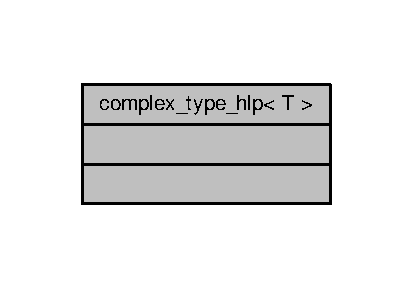
\includegraphics[width=198pt]{structcomplex__type__hlp__coll__graph}
\end{center}
\end{figure}


The documentation for this struct was generated from the following file\-:\begin{DoxyCompactItemize}
\item 
source/external\-\_\-libraries/\hyperlink{cufft__wrap_8h}{cufft\-\_\-wrap.\-h}\end{DoxyCompactItemize}

\hypertarget{structcomplex__type__hlp_3_01double_01_4}{\section{complex\-\_\-type\-\_\-hlp$<$ double $>$ Struct Template Reference}
\label{structcomplex__type__hlp_3_01double_01_4}\index{complex\-\_\-type\-\_\-hlp$<$ double $>$@{complex\-\_\-type\-\_\-hlp$<$ double $>$}}
}


{\ttfamily \#include $<$cufft\-\_\-wrap.\-h$>$}



Collaboration diagram for complex\-\_\-type\-\_\-hlp$<$ double $>$\-:\nopagebreak
\begin{figure}[H]
\begin{center}
\leavevmode
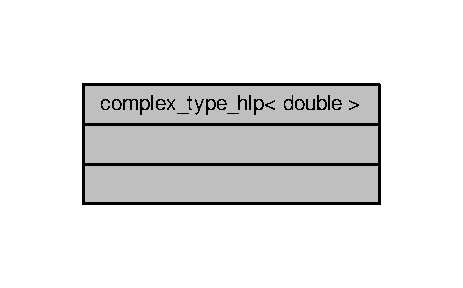
\includegraphics[width=222pt]{structcomplex__type__hlp_3_01double_01_4__coll__graph}
\end{center}
\end{figure}
\subsection*{Public Types}
\begin{DoxyCompactItemize}
\item 
typedef cufft\-Double\-Complex \hyperlink{structcomplex__type__hlp_3_01double_01_4_ab7bf6a2f6317b455665124fe54c356e2}{type}
\end{DoxyCompactItemize}


\subsection{Member Typedef Documentation}
\hypertarget{structcomplex__type__hlp_3_01double_01_4_ab7bf6a2f6317b455665124fe54c356e2}{\index{complex\-\_\-type\-\_\-hlp$<$ double $>$@{complex\-\_\-type\-\_\-hlp$<$ double $>$}!type@{type}}
\index{type@{type}!complex_type_hlp< double >@{complex\-\_\-type\-\_\-hlp$<$ double $>$}}
\subsubsection[{type}]{\setlength{\rightskip}{0pt plus 5cm}typedef cufft\-Double\-Complex {\bf complex\-\_\-type\-\_\-hlp}$<$ double $>$\-::{\bf type}}}\label{structcomplex__type__hlp_3_01double_01_4_ab7bf6a2f6317b455665124fe54c356e2}


The documentation for this struct was generated from the following file\-:\begin{DoxyCompactItemize}
\item 
source/external\-\_\-libraries/\hyperlink{cufft__wrap_8h}{cufft\-\_\-wrap.\-h}\end{DoxyCompactItemize}

\hypertarget{structcomplex__type__hlp_3_01float_01_4}{\section{complex\-\_\-type\-\_\-hlp$<$ float $>$ Struct Template Reference}
\label{structcomplex__type__hlp_3_01float_01_4}\index{complex\-\_\-type\-\_\-hlp$<$ float $>$@{complex\-\_\-type\-\_\-hlp$<$ float $>$}}
}


{\ttfamily \#include $<$cufft\-\_\-wrap.\-h$>$}



Collaboration diagram for complex\-\_\-type\-\_\-hlp$<$ float $>$\-:
\nopagebreak
\begin{figure}[H]
\begin{center}
\leavevmode
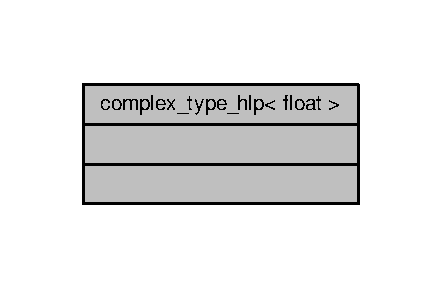
\includegraphics[width=212pt]{structcomplex__type__hlp_3_01float_01_4__coll__graph}
\end{center}
\end{figure}
\subsection*{Public Types}
\begin{DoxyCompactItemize}
\item 
typedef cufft\-Complex \hyperlink{structcomplex__type__hlp_3_01float_01_4_ae0cfcbdeb31ff876914355874c131ceb}{type}
\end{DoxyCompactItemize}


\subsection{Member Typedef Documentation}
\hypertarget{structcomplex__type__hlp_3_01float_01_4_ae0cfcbdeb31ff876914355874c131ceb}{\index{complex\-\_\-type\-\_\-hlp$<$ float $>$@{complex\-\_\-type\-\_\-hlp$<$ float $>$}!type@{type}}
\index{type@{type}!complex_type_hlp< float >@{complex\-\_\-type\-\_\-hlp$<$ float $>$}}
\subsubsection[{type}]{\setlength{\rightskip}{0pt plus 5cm}typedef cufft\-Complex {\bf complex\-\_\-type\-\_\-hlp}$<$ float $>$\-::{\bf type}}}\label{structcomplex__type__hlp_3_01float_01_4_ae0cfcbdeb31ff876914355874c131ceb}


The documentation for this struct was generated from the following file\-:\begin{DoxyCompactItemize}
\item 
source/external\-\_\-libraries/\hyperlink{cufft__wrap_8h}{cufft\-\_\-wrap.\-h}\end{DoxyCompactItemize}

\hypertarget{classcontinuation_1_1newton__method__extended_1_1convergence__strategy}{\section{continuation\-:\-:newton\-\_\-method\-\_\-extended\-:\-:convergence\-\_\-strategy$<$ vector\-\_\-operations, nonlinear\-\_\-operator, logging $>$ Class Template Reference}
\label{classcontinuation_1_1newton__method__extended_1_1convergence__strategy}\index{continuation\-::newton\-\_\-method\-\_\-extended\-::convergence\-\_\-strategy$<$ vector\-\_\-operations, nonlinear\-\_\-operator, logging $>$@{continuation\-::newton\-\_\-method\-\_\-extended\-::convergence\-\_\-strategy$<$ vector\-\_\-operations, nonlinear\-\_\-operator, logging $>$}}
}


{\ttfamily \#include $<$convergence\-\_\-strategy.\-h$>$}



Collaboration diagram for continuation\-:\-:newton\-\_\-method\-\_\-extended\-:\-:convergence\-\_\-strategy$<$ vector\-\_\-operations, nonlinear\-\_\-operator, logging $>$\-:
\nopagebreak
\begin{figure}[H]
\begin{center}
\leavevmode
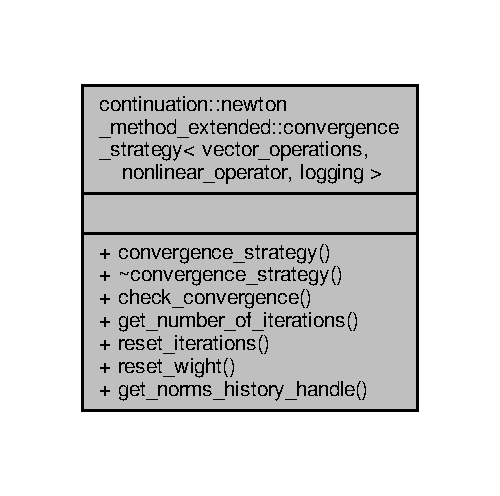
\includegraphics[width=240pt]{classcontinuation_1_1newton__method__extended_1_1convergence__strategy__coll__graph}
\end{center}
\end{figure}
\subsection*{Public Member Functions}
\begin{DoxyCompactItemize}
\item 
\hyperlink{classcontinuation_1_1newton__method__extended_1_1convergence__strategy_a445baea2c85ff055bd56cf759137b348}{convergence\-\_\-strategy} (\hyperlink{container__test_8cpp_aca3cc0310428d338f3a165c7823d6499}{vector\-\_\-operations} $\ast$\&vec\-\_\-ops\-\_\-, logging $\ast$\&log\-\_\-, T tolerance\-\_\-, unsigned \hyperlink{classint}{int} maximum\-\_\-iterations\-\_\-, T newton\-\_\-wight\-\_\-, bool store\-\_\-norms\-\_\-history\-\_\-=false, bool verbose\-\_\-=true)
\item 
\hyperlink{classcontinuation_1_1newton__method__extended_1_1convergence__strategy_aa825f21fb3d1a30084300840aae2597d}{$\sim$convergence\-\_\-strategy} ()
\item 
bool \hyperlink{classcontinuation_1_1newton__method__extended_1_1convergence__strategy_a054b5c56e77943cedf093b6e6513cb64}{check\-\_\-convergence} (nonlinear\-\_\-operator$\ast$nonlin\-\_\-op, T\-\_\-vec \&x, T \&lambda, T\-\_\-vec \&delta\-\_\-x, T \&delta\-\_\-lambda, \hyperlink{classint}{int} \&result\-\_\-status)
\item 
unsigned \hyperlink{classint}{int} \hyperlink{classcontinuation_1_1newton__method__extended_1_1convergence__strategy_a2df8e2aee0729595a75f05af99a4ad52}{get\-\_\-number\-\_\-of\-\_\-iterations} ()
\item 
void \hyperlink{classcontinuation_1_1newton__method__extended_1_1convergence__strategy_aac6e6e797796f2140672e5a9e5b548ca}{reset\-\_\-iterations} ()
\item 
void \hyperlink{classcontinuation_1_1newton__method__extended_1_1convergence__strategy_ac2970259c99acefb3ab55dbceaae94d2}{reset\-\_\-wight} ()
\item 
std\-::vector$<$ T $>$ $\ast$ \hyperlink{classcontinuation_1_1newton__method__extended_1_1convergence__strategy_ad3d8047988b42c57ad698321ea3eb065}{get\-\_\-norms\-\_\-history\-\_\-handle} ()
\end{DoxyCompactItemize}


\subsection{Constructor \& Destructor Documentation}
\hypertarget{classcontinuation_1_1newton__method__extended_1_1convergence__strategy_a445baea2c85ff055bd56cf759137b348}{\index{continuation\-::newton\-\_\-method\-\_\-extended\-::convergence\-\_\-strategy@{continuation\-::newton\-\_\-method\-\_\-extended\-::convergence\-\_\-strategy}!convergence\-\_\-strategy@{convergence\-\_\-strategy}}
\index{convergence\-\_\-strategy@{convergence\-\_\-strategy}!continuation::newton_method_extended::convergence_strategy@{continuation\-::newton\-\_\-method\-\_\-extended\-::convergence\-\_\-strategy}}
\subsubsection[{convergence\-\_\-strategy}]{\setlength{\rightskip}{0pt plus 5cm}template$<$class vector\-\_\-operations , class nonlinear\-\_\-operator , class logging $>$ {\bf continuation\-::newton\-\_\-method\-\_\-extended\-::convergence\-\_\-strategy}$<$ {\bf vector\-\_\-operations}, nonlinear\-\_\-operator, logging $>$\-::{\bf convergence\-\_\-strategy} (
\begin{DoxyParamCaption}
\item[{{\bf vector\-\_\-operations} $\ast$\&}]{vec\-\_\-ops\-\_\-, }
\item[{logging $\ast$\&}]{log\-\_\-, }
\item[{T}]{tolerance\-\_\-, }
\item[{unsigned {\bf int}}]{maximum\-\_\-iterations\-\_\-, }
\item[{T}]{newton\-\_\-wight\-\_\-, }
\item[{bool}]{store\-\_\-norms\-\_\-history\-\_\- = {\ttfamily false}, }
\item[{bool}]{verbose\-\_\- = {\ttfamily true}}
\end{DoxyParamCaption}
)\hspace{0.3cm}{\ttfamily [inline]}}}\label{classcontinuation_1_1newton__method__extended_1_1convergence__strategy_a445baea2c85ff055bd56cf759137b348}


Here is the call graph for this function\-:
\nopagebreak
\begin{figure}[H]
\begin{center}
\leavevmode
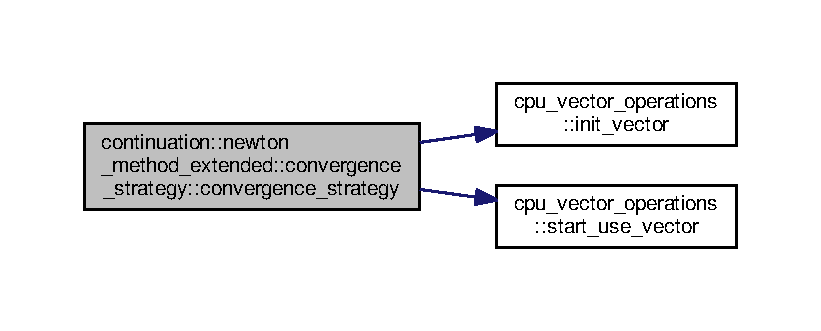
\includegraphics[width=350pt]{classcontinuation_1_1newton__method__extended_1_1convergence__strategy_a445baea2c85ff055bd56cf759137b348_cgraph}
\end{center}
\end{figure}


\hypertarget{classcontinuation_1_1newton__method__extended_1_1convergence__strategy_aa825f21fb3d1a30084300840aae2597d}{\index{continuation\-::newton\-\_\-method\-\_\-extended\-::convergence\-\_\-strategy@{continuation\-::newton\-\_\-method\-\_\-extended\-::convergence\-\_\-strategy}!$\sim$convergence\-\_\-strategy@{$\sim$convergence\-\_\-strategy}}
\index{$\sim$convergence\-\_\-strategy@{$\sim$convergence\-\_\-strategy}!continuation::newton_method_extended::convergence_strategy@{continuation\-::newton\-\_\-method\-\_\-extended\-::convergence\-\_\-strategy}}
\subsubsection[{$\sim$convergence\-\_\-strategy}]{\setlength{\rightskip}{0pt plus 5cm}template$<$class vector\-\_\-operations , class nonlinear\-\_\-operator , class logging $>$ {\bf continuation\-::newton\-\_\-method\-\_\-extended\-::convergence\-\_\-strategy}$<$ {\bf vector\-\_\-operations}, nonlinear\-\_\-operator, logging $>$\-::$\sim${\bf convergence\-\_\-strategy} (
\begin{DoxyParamCaption}
{}
\end{DoxyParamCaption}
)\hspace{0.3cm}{\ttfamily [inline]}}}\label{classcontinuation_1_1newton__method__extended_1_1convergence__strategy_aa825f21fb3d1a30084300840aae2597d}


Here is the call graph for this function\-:
\nopagebreak
\begin{figure}[H]
\begin{center}
\leavevmode
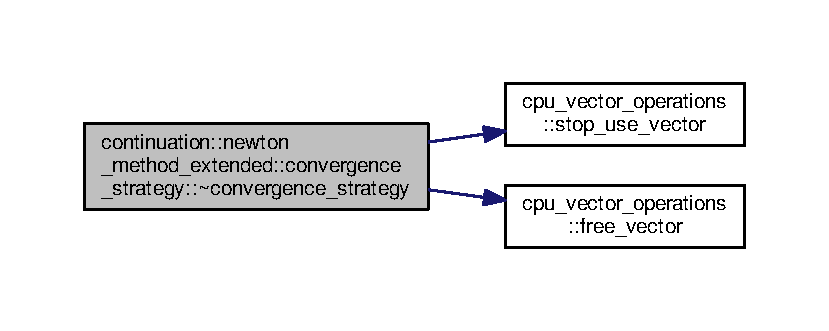
\includegraphics[width=350pt]{classcontinuation_1_1newton__method__extended_1_1convergence__strategy_aa825f21fb3d1a30084300840aae2597d_cgraph}
\end{center}
\end{figure}




\subsection{Member Function Documentation}
\hypertarget{classcontinuation_1_1newton__method__extended_1_1convergence__strategy_a054b5c56e77943cedf093b6e6513cb64}{\index{continuation\-::newton\-\_\-method\-\_\-extended\-::convergence\-\_\-strategy@{continuation\-::newton\-\_\-method\-\_\-extended\-::convergence\-\_\-strategy}!check\-\_\-convergence@{check\-\_\-convergence}}
\index{check\-\_\-convergence@{check\-\_\-convergence}!continuation::newton_method_extended::convergence_strategy@{continuation\-::newton\-\_\-method\-\_\-extended\-::convergence\-\_\-strategy}}
\subsubsection[{check\-\_\-convergence}]{\setlength{\rightskip}{0pt plus 5cm}template$<$class vector\-\_\-operations , class nonlinear\-\_\-operator , class logging $>$ bool {\bf continuation\-::newton\-\_\-method\-\_\-extended\-::convergence\-\_\-strategy}$<$ {\bf vector\-\_\-operations}, nonlinear\-\_\-operator, logging $>$\-::check\-\_\-convergence (
\begin{DoxyParamCaption}
\item[{nonlinear\-\_\-operator$\ast$}]{nonlin\-\_\-op, }
\item[{T\-\_\-vec \&}]{x, }
\item[{T \&}]{lambda, }
\item[{T\-\_\-vec \&}]{delta\-\_\-x, }
\item[{T \&}]{delta\-\_\-lambda, }
\item[{{\bf int} \&}]{result\-\_\-status}
\end{DoxyParamCaption}
)\hspace{0.3cm}{\ttfamily [inline]}}}\label{classcontinuation_1_1newton__method__extended_1_1convergence__strategy_a054b5c56e77943cedf093b6e6513cb64}


Here is the call graph for this function\-:
\nopagebreak
\begin{figure}[H]
\begin{center}
\leavevmode
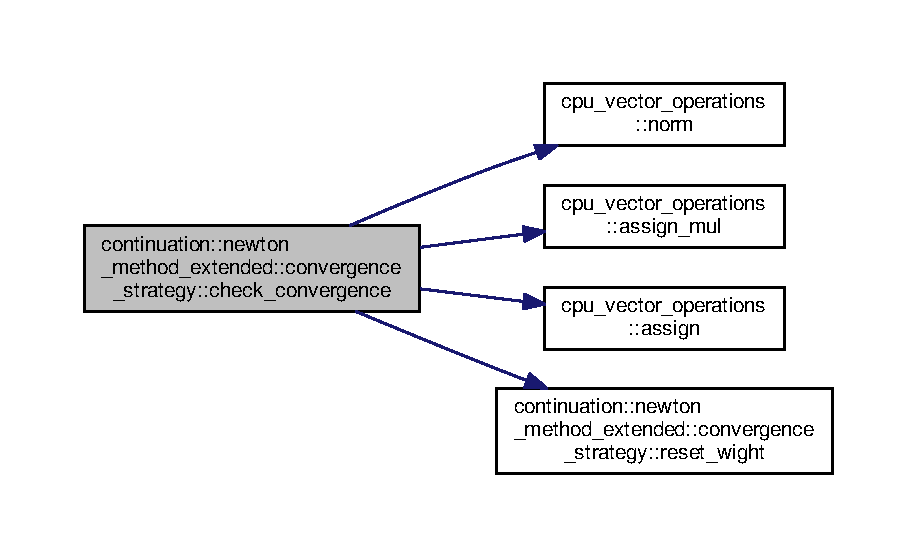
\includegraphics[width=350pt]{classcontinuation_1_1newton__method__extended_1_1convergence__strategy_a054b5c56e77943cedf093b6e6513cb64_cgraph}
\end{center}
\end{figure}


\hypertarget{classcontinuation_1_1newton__method__extended_1_1convergence__strategy_ad3d8047988b42c57ad698321ea3eb065}{\index{continuation\-::newton\-\_\-method\-\_\-extended\-::convergence\-\_\-strategy@{continuation\-::newton\-\_\-method\-\_\-extended\-::convergence\-\_\-strategy}!get\-\_\-norms\-\_\-history\-\_\-handle@{get\-\_\-norms\-\_\-history\-\_\-handle}}
\index{get\-\_\-norms\-\_\-history\-\_\-handle@{get\-\_\-norms\-\_\-history\-\_\-handle}!continuation::newton_method_extended::convergence_strategy@{continuation\-::newton\-\_\-method\-\_\-extended\-::convergence\-\_\-strategy}}
\subsubsection[{get\-\_\-norms\-\_\-history\-\_\-handle}]{\setlength{\rightskip}{0pt plus 5cm}template$<$class vector\-\_\-operations , class nonlinear\-\_\-operator , class logging $>$ std\-::vector$<$T$>$$\ast$ {\bf continuation\-::newton\-\_\-method\-\_\-extended\-::convergence\-\_\-strategy}$<$ {\bf vector\-\_\-operations}, nonlinear\-\_\-operator, logging $>$\-::get\-\_\-norms\-\_\-history\-\_\-handle (
\begin{DoxyParamCaption}
{}
\end{DoxyParamCaption}
)\hspace{0.3cm}{\ttfamily [inline]}}}\label{classcontinuation_1_1newton__method__extended_1_1convergence__strategy_ad3d8047988b42c57ad698321ea3eb065}
\hypertarget{classcontinuation_1_1newton__method__extended_1_1convergence__strategy_a2df8e2aee0729595a75f05af99a4ad52}{\index{continuation\-::newton\-\_\-method\-\_\-extended\-::convergence\-\_\-strategy@{continuation\-::newton\-\_\-method\-\_\-extended\-::convergence\-\_\-strategy}!get\-\_\-number\-\_\-of\-\_\-iterations@{get\-\_\-number\-\_\-of\-\_\-iterations}}
\index{get\-\_\-number\-\_\-of\-\_\-iterations@{get\-\_\-number\-\_\-of\-\_\-iterations}!continuation::newton_method_extended::convergence_strategy@{continuation\-::newton\-\_\-method\-\_\-extended\-::convergence\-\_\-strategy}}
\subsubsection[{get\-\_\-number\-\_\-of\-\_\-iterations}]{\setlength{\rightskip}{0pt plus 5cm}template$<$class vector\-\_\-operations , class nonlinear\-\_\-operator , class logging $>$ unsigned {\bf int} {\bf continuation\-::newton\-\_\-method\-\_\-extended\-::convergence\-\_\-strategy}$<$ {\bf vector\-\_\-operations}, nonlinear\-\_\-operator, logging $>$\-::get\-\_\-number\-\_\-of\-\_\-iterations (
\begin{DoxyParamCaption}
{}
\end{DoxyParamCaption}
)\hspace{0.3cm}{\ttfamily [inline]}}}\label{classcontinuation_1_1newton__method__extended_1_1convergence__strategy_a2df8e2aee0729595a75f05af99a4ad52}
\hypertarget{classcontinuation_1_1newton__method__extended_1_1convergence__strategy_aac6e6e797796f2140672e5a9e5b548ca}{\index{continuation\-::newton\-\_\-method\-\_\-extended\-::convergence\-\_\-strategy@{continuation\-::newton\-\_\-method\-\_\-extended\-::convergence\-\_\-strategy}!reset\-\_\-iterations@{reset\-\_\-iterations}}
\index{reset\-\_\-iterations@{reset\-\_\-iterations}!continuation::newton_method_extended::convergence_strategy@{continuation\-::newton\-\_\-method\-\_\-extended\-::convergence\-\_\-strategy}}
\subsubsection[{reset\-\_\-iterations}]{\setlength{\rightskip}{0pt plus 5cm}template$<$class vector\-\_\-operations , class nonlinear\-\_\-operator , class logging $>$ void {\bf continuation\-::newton\-\_\-method\-\_\-extended\-::convergence\-\_\-strategy}$<$ {\bf vector\-\_\-operations}, nonlinear\-\_\-operator, logging $>$\-::reset\-\_\-iterations (
\begin{DoxyParamCaption}
{}
\end{DoxyParamCaption}
)\hspace{0.3cm}{\ttfamily [inline]}}}\label{classcontinuation_1_1newton__method__extended_1_1convergence__strategy_aac6e6e797796f2140672e5a9e5b548ca}


Here is the call graph for this function\-:
\nopagebreak
\begin{figure}[H]
\begin{center}
\leavevmode
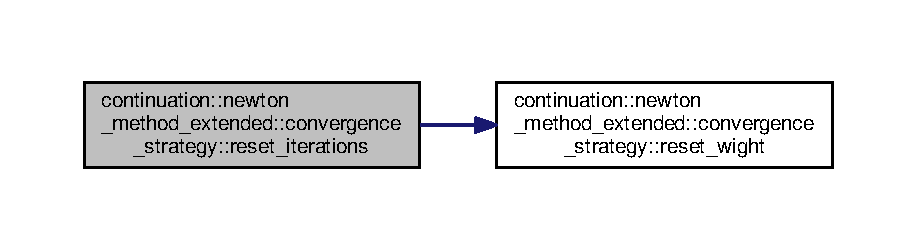
\includegraphics[width=350pt]{classcontinuation_1_1newton__method__extended_1_1convergence__strategy_aac6e6e797796f2140672e5a9e5b548ca_cgraph}
\end{center}
\end{figure}


\hypertarget{classcontinuation_1_1newton__method__extended_1_1convergence__strategy_ac2970259c99acefb3ab55dbceaae94d2}{\index{continuation\-::newton\-\_\-method\-\_\-extended\-::convergence\-\_\-strategy@{continuation\-::newton\-\_\-method\-\_\-extended\-::convergence\-\_\-strategy}!reset\-\_\-wight@{reset\-\_\-wight}}
\index{reset\-\_\-wight@{reset\-\_\-wight}!continuation::newton_method_extended::convergence_strategy@{continuation\-::newton\-\_\-method\-\_\-extended\-::convergence\-\_\-strategy}}
\subsubsection[{reset\-\_\-wight}]{\setlength{\rightskip}{0pt plus 5cm}template$<$class vector\-\_\-operations , class nonlinear\-\_\-operator , class logging $>$ void {\bf continuation\-::newton\-\_\-method\-\_\-extended\-::convergence\-\_\-strategy}$<$ {\bf vector\-\_\-operations}, nonlinear\-\_\-operator, logging $>$\-::reset\-\_\-wight (
\begin{DoxyParamCaption}
{}
\end{DoxyParamCaption}
)\hspace{0.3cm}{\ttfamily [inline]}}}\label{classcontinuation_1_1newton__method__extended_1_1convergence__strategy_ac2970259c99acefb3ab55dbceaae94d2}


Here is the caller graph for this function\-:
\nopagebreak
\begin{figure}[H]
\begin{center}
\leavevmode
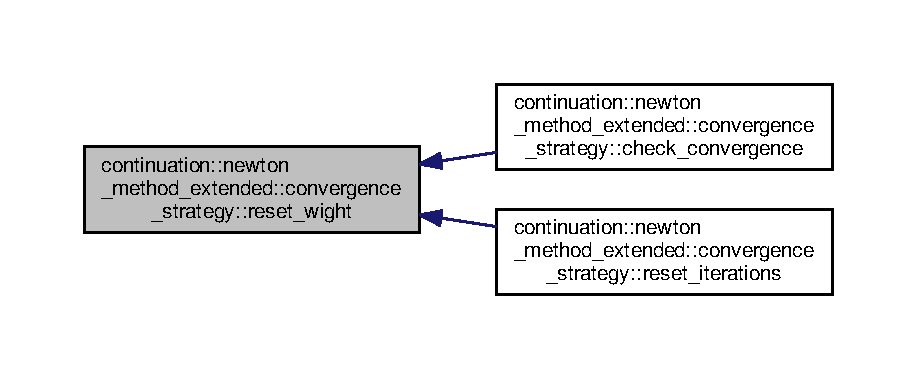
\includegraphics[width=350pt]{classcontinuation_1_1newton__method__extended_1_1convergence__strategy_ac2970259c99acefb3ab55dbceaae94d2_icgraph}
\end{center}
\end{figure}




The documentation for this class was generated from the following file\-:\begin{DoxyCompactItemize}
\item 
source/continuation/\hyperlink{continuation_2convergence__strategy_8h}{convergence\-\_\-strategy.\-h}\end{DoxyCompactItemize}

\hypertarget{classdeflation_1_1newton__method__extended_1_1convergence__strategy}{\section{deflation\-:\-:newton\-\_\-method\-\_\-extended\-:\-:convergence\-\_\-strategy$<$ Vector\-Operations, Nonlinear\-Operator, Logging $>$ Class Template Reference}
\label{classdeflation_1_1newton__method__extended_1_1convergence__strategy}\index{deflation\-::newton\-\_\-method\-\_\-extended\-::convergence\-\_\-strategy$<$ Vector\-Operations, Nonlinear\-Operator, Logging $>$@{deflation\-::newton\-\_\-method\-\_\-extended\-::convergence\-\_\-strategy$<$ Vector\-Operations, Nonlinear\-Operator, Logging $>$}}
}


{\ttfamily \#include $<$convergence\-\_\-strategy.\-h$>$}



Collaboration diagram for deflation\-:\-:newton\-\_\-method\-\_\-extended\-:\-:convergence\-\_\-strategy$<$ Vector\-Operations, Nonlinear\-Operator, Logging $>$\-:
\nopagebreak
\begin{figure}[H]
\begin{center}
\leavevmode
\includegraphics[width=226pt]{classdeflation_1_1newton__method__extended_1_1convergence__strategy__coll__graph}
\end{center}
\end{figure}
\subsection*{Public Member Functions}
\begin{DoxyCompactItemize}
\item 
\hyperlink{classdeflation_1_1newton__method__extended_1_1convergence__strategy_a9ca9cf9f688586ed07f00395bae6e668}{convergence\-\_\-strategy} (Vector\-Operations $\ast$\&vec\-\_\-ops\-\_\-, Logging $\ast$\&log\-\_\-, T tolerance\-\_\-, unsigned \hyperlink{classint}{int} maximum\-\_\-iterations\-\_\-, T newton\-\_\-wight\-\_\-, bool store\-\_\-norms\-\_\-history\-\_\-=false, bool verbose\-\_\-=true)
\item 
\hyperlink{classdeflation_1_1newton__method__extended_1_1convergence__strategy_a34c8b595e91495861191123ef90d0d4b}{$\sim$convergence\-\_\-strategy} ()
\item 
bool \hyperlink{classdeflation_1_1newton__method__extended_1_1convergence__strategy_a537bfe541b97eb6810d9f72a951d44cc}{check\-\_\-convergence} (Nonlinear\-Operator $\ast$nonlin\-\_\-op, T\-\_\-vec \&x, T \&lambda, T\-\_\-vec \&delta\-\_\-x, T \&delta\-\_\-lambda, \hyperlink{classint}{int} \&result\-\_\-status)
\item 
unsigned \hyperlink{classint}{int} \hyperlink{classdeflation_1_1newton__method__extended_1_1convergence__strategy_a9d9ce3025cff7f1aec33e44da85f1526}{get\-\_\-number\-\_\-of\-\_\-iterations} ()
\item 
void \hyperlink{classdeflation_1_1newton__method__extended_1_1convergence__strategy_ac7a2306183d029d7c865a49d55e01425}{reset\-\_\-iterations} ()
\item 
void \hyperlink{classdeflation_1_1newton__method__extended_1_1convergence__strategy_a7dc80cfafdb7057cc10b5f05bb1e287a}{reset\-\_\-wight} ()
\item 
std\-::vector$<$ T $>$ $\ast$ \hyperlink{classdeflation_1_1newton__method__extended_1_1convergence__strategy_a325a124ea85d1ae522d3d1fe24c28b9c}{get\-\_\-norms\-\_\-history\-\_\-handle} ()
\end{DoxyCompactItemize}


\subsection{Constructor \& Destructor Documentation}
\hypertarget{classdeflation_1_1newton__method__extended_1_1convergence__strategy_a9ca9cf9f688586ed07f00395bae6e668}{\index{deflation\-::newton\-\_\-method\-\_\-extended\-::convergence\-\_\-strategy@{deflation\-::newton\-\_\-method\-\_\-extended\-::convergence\-\_\-strategy}!convergence\-\_\-strategy@{convergence\-\_\-strategy}}
\index{convergence\-\_\-strategy@{convergence\-\_\-strategy}!deflation::newton_method_extended::convergence_strategy@{deflation\-::newton\-\_\-method\-\_\-extended\-::convergence\-\_\-strategy}}
\subsubsection[{convergence\-\_\-strategy}]{\setlength{\rightskip}{0pt plus 5cm}template$<$class Vector\-Operations , class Nonlinear\-Operator , class Logging $>$ {\bf deflation\-::newton\-\_\-method\-\_\-extended\-::convergence\-\_\-strategy}$<$ Vector\-Operations, Nonlinear\-Operator, Logging $>$\-::{\bf convergence\-\_\-strategy} (
\begin{DoxyParamCaption}
\item[{Vector\-Operations $\ast$\&}]{vec\-\_\-ops\-\_\-, }
\item[{Logging $\ast$\&}]{log\-\_\-, }
\item[{T}]{tolerance\-\_\-, }
\item[{unsigned {\bf int}}]{maximum\-\_\-iterations\-\_\-, }
\item[{T}]{newton\-\_\-wight\-\_\-, }
\item[{bool}]{store\-\_\-norms\-\_\-history\-\_\- = {\ttfamily false}, }
\item[{bool}]{verbose\-\_\- = {\ttfamily true}}
\end{DoxyParamCaption}
)\hspace{0.3cm}{\ttfamily [inline]}}}\label{classdeflation_1_1newton__method__extended_1_1convergence__strategy_a9ca9cf9f688586ed07f00395bae6e668}
\hypertarget{classdeflation_1_1newton__method__extended_1_1convergence__strategy_a34c8b595e91495861191123ef90d0d4b}{\index{deflation\-::newton\-\_\-method\-\_\-extended\-::convergence\-\_\-strategy@{deflation\-::newton\-\_\-method\-\_\-extended\-::convergence\-\_\-strategy}!$\sim$convergence\-\_\-strategy@{$\sim$convergence\-\_\-strategy}}
\index{$\sim$convergence\-\_\-strategy@{$\sim$convergence\-\_\-strategy}!deflation::newton_method_extended::convergence_strategy@{deflation\-::newton\-\_\-method\-\_\-extended\-::convergence\-\_\-strategy}}
\subsubsection[{$\sim$convergence\-\_\-strategy}]{\setlength{\rightskip}{0pt plus 5cm}template$<$class Vector\-Operations , class Nonlinear\-Operator , class Logging $>$ {\bf deflation\-::newton\-\_\-method\-\_\-extended\-::convergence\-\_\-strategy}$<$ Vector\-Operations, Nonlinear\-Operator, Logging $>$\-::$\sim${\bf convergence\-\_\-strategy} (
\begin{DoxyParamCaption}
{}
\end{DoxyParamCaption}
)\hspace{0.3cm}{\ttfamily [inline]}}}\label{classdeflation_1_1newton__method__extended_1_1convergence__strategy_a34c8b595e91495861191123ef90d0d4b}


\subsection{Member Function Documentation}
\hypertarget{classdeflation_1_1newton__method__extended_1_1convergence__strategy_a537bfe541b97eb6810d9f72a951d44cc}{\index{deflation\-::newton\-\_\-method\-\_\-extended\-::convergence\-\_\-strategy@{deflation\-::newton\-\_\-method\-\_\-extended\-::convergence\-\_\-strategy}!check\-\_\-convergence@{check\-\_\-convergence}}
\index{check\-\_\-convergence@{check\-\_\-convergence}!deflation::newton_method_extended::convergence_strategy@{deflation\-::newton\-\_\-method\-\_\-extended\-::convergence\-\_\-strategy}}
\subsubsection[{check\-\_\-convergence}]{\setlength{\rightskip}{0pt plus 5cm}template$<$class Vector\-Operations , class Nonlinear\-Operator , class Logging $>$ bool {\bf deflation\-::newton\-\_\-method\-\_\-extended\-::convergence\-\_\-strategy}$<$ Vector\-Operations, Nonlinear\-Operator, Logging $>$\-::check\-\_\-convergence (
\begin{DoxyParamCaption}
\item[{Nonlinear\-Operator $\ast$}]{nonlin\-\_\-op, }
\item[{T\-\_\-vec \&}]{x, }
\item[{T \&}]{lambda, }
\item[{T\-\_\-vec \&}]{delta\-\_\-x, }
\item[{T \&}]{delta\-\_\-lambda, }
\item[{{\bf int} \&}]{result\-\_\-status}
\end{DoxyParamCaption}
)\hspace{0.3cm}{\ttfamily [inline]}}}\label{classdeflation_1_1newton__method__extended_1_1convergence__strategy_a537bfe541b97eb6810d9f72a951d44cc}
\hypertarget{classdeflation_1_1newton__method__extended_1_1convergence__strategy_a325a124ea85d1ae522d3d1fe24c28b9c}{\index{deflation\-::newton\-\_\-method\-\_\-extended\-::convergence\-\_\-strategy@{deflation\-::newton\-\_\-method\-\_\-extended\-::convergence\-\_\-strategy}!get\-\_\-norms\-\_\-history\-\_\-handle@{get\-\_\-norms\-\_\-history\-\_\-handle}}
\index{get\-\_\-norms\-\_\-history\-\_\-handle@{get\-\_\-norms\-\_\-history\-\_\-handle}!deflation::newton_method_extended::convergence_strategy@{deflation\-::newton\-\_\-method\-\_\-extended\-::convergence\-\_\-strategy}}
\subsubsection[{get\-\_\-norms\-\_\-history\-\_\-handle}]{\setlength{\rightskip}{0pt plus 5cm}template$<$class Vector\-Operations , class Nonlinear\-Operator , class Logging $>$ std\-::vector$<$T$>$$\ast$ {\bf deflation\-::newton\-\_\-method\-\_\-extended\-::convergence\-\_\-strategy}$<$ Vector\-Operations, Nonlinear\-Operator, Logging $>$\-::get\-\_\-norms\-\_\-history\-\_\-handle (
\begin{DoxyParamCaption}
{}
\end{DoxyParamCaption}
)\hspace{0.3cm}{\ttfamily [inline]}}}\label{classdeflation_1_1newton__method__extended_1_1convergence__strategy_a325a124ea85d1ae522d3d1fe24c28b9c}
\hypertarget{classdeflation_1_1newton__method__extended_1_1convergence__strategy_a9d9ce3025cff7f1aec33e44da85f1526}{\index{deflation\-::newton\-\_\-method\-\_\-extended\-::convergence\-\_\-strategy@{deflation\-::newton\-\_\-method\-\_\-extended\-::convergence\-\_\-strategy}!get\-\_\-number\-\_\-of\-\_\-iterations@{get\-\_\-number\-\_\-of\-\_\-iterations}}
\index{get\-\_\-number\-\_\-of\-\_\-iterations@{get\-\_\-number\-\_\-of\-\_\-iterations}!deflation::newton_method_extended::convergence_strategy@{deflation\-::newton\-\_\-method\-\_\-extended\-::convergence\-\_\-strategy}}
\subsubsection[{get\-\_\-number\-\_\-of\-\_\-iterations}]{\setlength{\rightskip}{0pt plus 5cm}template$<$class Vector\-Operations , class Nonlinear\-Operator , class Logging $>$ unsigned {\bf int} {\bf deflation\-::newton\-\_\-method\-\_\-extended\-::convergence\-\_\-strategy}$<$ Vector\-Operations, Nonlinear\-Operator, Logging $>$\-::get\-\_\-number\-\_\-of\-\_\-iterations (
\begin{DoxyParamCaption}
{}
\end{DoxyParamCaption}
)\hspace{0.3cm}{\ttfamily [inline]}}}\label{classdeflation_1_1newton__method__extended_1_1convergence__strategy_a9d9ce3025cff7f1aec33e44da85f1526}
\hypertarget{classdeflation_1_1newton__method__extended_1_1convergence__strategy_ac7a2306183d029d7c865a49d55e01425}{\index{deflation\-::newton\-\_\-method\-\_\-extended\-::convergence\-\_\-strategy@{deflation\-::newton\-\_\-method\-\_\-extended\-::convergence\-\_\-strategy}!reset\-\_\-iterations@{reset\-\_\-iterations}}
\index{reset\-\_\-iterations@{reset\-\_\-iterations}!deflation::newton_method_extended::convergence_strategy@{deflation\-::newton\-\_\-method\-\_\-extended\-::convergence\-\_\-strategy}}
\subsubsection[{reset\-\_\-iterations}]{\setlength{\rightskip}{0pt plus 5cm}template$<$class Vector\-Operations , class Nonlinear\-Operator , class Logging $>$ void {\bf deflation\-::newton\-\_\-method\-\_\-extended\-::convergence\-\_\-strategy}$<$ Vector\-Operations, Nonlinear\-Operator, Logging $>$\-::reset\-\_\-iterations (
\begin{DoxyParamCaption}
{}
\end{DoxyParamCaption}
)\hspace{0.3cm}{\ttfamily [inline]}}}\label{classdeflation_1_1newton__method__extended_1_1convergence__strategy_ac7a2306183d029d7c865a49d55e01425}


Here is the call graph for this function\-:
\nopagebreak
\begin{figure}[H]
\begin{center}
\leavevmode
\includegraphics[width=350pt]{classdeflation_1_1newton__method__extended_1_1convergence__strategy_ac7a2306183d029d7c865a49d55e01425_cgraph}
\end{center}
\end{figure}


\hypertarget{classdeflation_1_1newton__method__extended_1_1convergence__strategy_a7dc80cfafdb7057cc10b5f05bb1e287a}{\index{deflation\-::newton\-\_\-method\-\_\-extended\-::convergence\-\_\-strategy@{deflation\-::newton\-\_\-method\-\_\-extended\-::convergence\-\_\-strategy}!reset\-\_\-wight@{reset\-\_\-wight}}
\index{reset\-\_\-wight@{reset\-\_\-wight}!deflation::newton_method_extended::convergence_strategy@{deflation\-::newton\-\_\-method\-\_\-extended\-::convergence\-\_\-strategy}}
\subsubsection[{reset\-\_\-wight}]{\setlength{\rightskip}{0pt plus 5cm}template$<$class Vector\-Operations , class Nonlinear\-Operator , class Logging $>$ void {\bf deflation\-::newton\-\_\-method\-\_\-extended\-::convergence\-\_\-strategy}$<$ Vector\-Operations, Nonlinear\-Operator, Logging $>$\-::reset\-\_\-wight (
\begin{DoxyParamCaption}
{}
\end{DoxyParamCaption}
)\hspace{0.3cm}{\ttfamily [inline]}}}\label{classdeflation_1_1newton__method__extended_1_1convergence__strategy_a7dc80cfafdb7057cc10b5f05bb1e287a}


Here is the caller graph for this function\-:
\nopagebreak
\begin{figure}[H]
\begin{center}
\leavevmode
\includegraphics[width=350pt]{classdeflation_1_1newton__method__extended_1_1convergence__strategy_a7dc80cfafdb7057cc10b5f05bb1e287a_icgraph}
\end{center}
\end{figure}




The documentation for this class was generated from the following file\-:\begin{DoxyCompactItemize}
\item 
source/deflation/\hyperlink{deflation_2convergence__strategy_8h}{convergence\-\_\-strategy.\-h}\end{DoxyCompactItemize}

\hypertarget{classnonlinear__operators_1_1newton__method_1_1convergence__strategy}{\section{nonlinear\-\_\-operators\-:\-:newton\-\_\-method\-:\-:convergence\-\_\-strategy$<$ vector\-\_\-operations, nonlinear\-\_\-operator, logging $>$ Class Template Reference}
\label{classnonlinear__operators_1_1newton__method_1_1convergence__strategy}\index{nonlinear\-\_\-operators\-::newton\-\_\-method\-::convergence\-\_\-strategy$<$ vector\-\_\-operations, nonlinear\-\_\-operator, logging $>$@{nonlinear\-\_\-operators\-::newton\-\_\-method\-::convergence\-\_\-strategy$<$ vector\-\_\-operations, nonlinear\-\_\-operator, logging $>$}}
}


{\ttfamily \#include $<$convergence\-\_\-strategy.\-h$>$}



Collaboration diagram for nonlinear\-\_\-operators\-:\-:newton\-\_\-method\-:\-:convergence\-\_\-strategy$<$ vector\-\_\-operations, nonlinear\-\_\-operator, logging $>$\-:\nopagebreak
\begin{figure}[H]
\begin{center}
\leavevmode
\includegraphics[width=232pt]{classnonlinear__operators_1_1newton__method_1_1convergence__strategy__coll__graph}
\end{center}
\end{figure}
\subsection*{Public Member Functions}
\begin{DoxyCompactItemize}
\item 
\hyperlink{classnonlinear__operators_1_1newton__method_1_1convergence__strategy_a00e18a10009c673718f85720cfd37f53}{convergence\-\_\-strategy} (\hyperlink{container__test_8cpp_aca3cc0310428d338f3a165c7823d6499}{vector\-\_\-operations} $\ast$\&vec\-\_\-ops\-\_\-, logging $\ast$\&log\-\_\-, T tolerance\-\_\-, unsigned \hyperlink{classint}{int} maximum\-\_\-iterations\-\_\-, T newton\-\_\-wight\-\_\-, bool store\-\_\-norms\-\_\-history\-\_\-=false, bool verbose\-\_\-=true)
\item 
\hyperlink{classnonlinear__operators_1_1newton__method_1_1convergence__strategy_a8c43cb374b68b7edaf5e9570beacde60}{$\sim$convergence\-\_\-strategy} ()
\item 
bool \hyperlink{classnonlinear__operators_1_1newton__method_1_1convergence__strategy_af14415fad7e86ef9c2bf3da72745f685}{check\-\_\-convergence} (nonlinear\-\_\-operator$\ast$nonlin\-\_\-op, T\-\_\-vec \&x, T lambda, T\-\_\-vec \&delta\-\_\-x, \hyperlink{classint}{int} \&result\-\_\-status)
\item 
unsigned \hyperlink{classint}{int} \hyperlink{classnonlinear__operators_1_1newton__method_1_1convergence__strategy_a4ffd50fbf3c7b4d624b217e854e51e3a}{get\-\_\-number\-\_\-of\-\_\-iterations} ()
\item 
void \hyperlink{classnonlinear__operators_1_1newton__method_1_1convergence__strategy_a5c24a88352363a49d2f93b74f41f5ba3}{reset\-\_\-iterations} ()
\item 
void \hyperlink{classnonlinear__operators_1_1newton__method_1_1convergence__strategy_a207705b48cf5c002f33f0bc6e4f2cdf2}{reset\-\_\-wight} ()
\item 
std\-::vector$<$ T $>$ $\ast$ \hyperlink{classnonlinear__operators_1_1newton__method_1_1convergence__strategy_a6e7c6939333bc5e34db93075f90f5944}{get\-\_\-norms\-\_\-history\-\_\-handle} ()
\end{DoxyCompactItemize}


\subsection{Constructor \& Destructor Documentation}
\hypertarget{classnonlinear__operators_1_1newton__method_1_1convergence__strategy_a00e18a10009c673718f85720cfd37f53}{\index{nonlinear\-\_\-operators\-::newton\-\_\-method\-::convergence\-\_\-strategy@{nonlinear\-\_\-operators\-::newton\-\_\-method\-::convergence\-\_\-strategy}!convergence\-\_\-strategy@{convergence\-\_\-strategy}}
\index{convergence\-\_\-strategy@{convergence\-\_\-strategy}!nonlinear_operators::newton_method::convergence_strategy@{nonlinear\-\_\-operators\-::newton\-\_\-method\-::convergence\-\_\-strategy}}
\subsubsection[{convergence\-\_\-strategy}]{\setlength{\rightskip}{0pt plus 5cm}template$<$class vector\-\_\-operations , class nonlinear\-\_\-operator , class logging $>$ {\bf nonlinear\-\_\-operators\-::newton\-\_\-method\-::convergence\-\_\-strategy}$<$ {\bf vector\-\_\-operations}, nonlinear\-\_\-operator, logging $>$\-::{\bf convergence\-\_\-strategy} (
\begin{DoxyParamCaption}
\item[{{\bf vector\-\_\-operations} $\ast$\&}]{vec\-\_\-ops\-\_\-, }
\item[{logging $\ast$\&}]{log\-\_\-, }
\item[{T}]{tolerance\-\_\-, }
\item[{unsigned {\bf int}}]{maximum\-\_\-iterations\-\_\-, }
\item[{T}]{newton\-\_\-wight\-\_\-, }
\item[{bool}]{store\-\_\-norms\-\_\-history\-\_\- = {\ttfamily false}, }
\item[{bool}]{verbose\-\_\- = {\ttfamily true}}
\end{DoxyParamCaption}
)\hspace{0.3cm}{\ttfamily [inline]}}}\label{classnonlinear__operators_1_1newton__method_1_1convergence__strategy_a00e18a10009c673718f85720cfd37f53}


Here is the call graph for this function\-:\nopagebreak
\begin{figure}[H]
\begin{center}
\leavevmode
\includegraphics[width=350pt]{classnonlinear__operators_1_1newton__method_1_1convergence__strategy_a00e18a10009c673718f85720cfd37f53_cgraph}
\end{center}
\end{figure}


\hypertarget{classnonlinear__operators_1_1newton__method_1_1convergence__strategy_a8c43cb374b68b7edaf5e9570beacde60}{\index{nonlinear\-\_\-operators\-::newton\-\_\-method\-::convergence\-\_\-strategy@{nonlinear\-\_\-operators\-::newton\-\_\-method\-::convergence\-\_\-strategy}!$\sim$convergence\-\_\-strategy@{$\sim$convergence\-\_\-strategy}}
\index{$\sim$convergence\-\_\-strategy@{$\sim$convergence\-\_\-strategy}!nonlinear_operators::newton_method::convergence_strategy@{nonlinear\-\_\-operators\-::newton\-\_\-method\-::convergence\-\_\-strategy}}
\subsubsection[{$\sim$convergence\-\_\-strategy}]{\setlength{\rightskip}{0pt plus 5cm}template$<$class vector\-\_\-operations , class nonlinear\-\_\-operator , class logging $>$ {\bf nonlinear\-\_\-operators\-::newton\-\_\-method\-::convergence\-\_\-strategy}$<$ {\bf vector\-\_\-operations}, nonlinear\-\_\-operator, logging $>$\-::$\sim${\bf convergence\-\_\-strategy} (
\begin{DoxyParamCaption}
{}
\end{DoxyParamCaption}
)\hspace{0.3cm}{\ttfamily [inline]}}}\label{classnonlinear__operators_1_1newton__method_1_1convergence__strategy_a8c43cb374b68b7edaf5e9570beacde60}


Here is the call graph for this function\-:\nopagebreak
\begin{figure}[H]
\begin{center}
\leavevmode
\includegraphics[width=350pt]{classnonlinear__operators_1_1newton__method_1_1convergence__strategy_a8c43cb374b68b7edaf5e9570beacde60_cgraph}
\end{center}
\end{figure}




\subsection{Member Function Documentation}
\hypertarget{classnonlinear__operators_1_1newton__method_1_1convergence__strategy_af14415fad7e86ef9c2bf3da72745f685}{\index{nonlinear\-\_\-operators\-::newton\-\_\-method\-::convergence\-\_\-strategy@{nonlinear\-\_\-operators\-::newton\-\_\-method\-::convergence\-\_\-strategy}!check\-\_\-convergence@{check\-\_\-convergence}}
\index{check\-\_\-convergence@{check\-\_\-convergence}!nonlinear_operators::newton_method::convergence_strategy@{nonlinear\-\_\-operators\-::newton\-\_\-method\-::convergence\-\_\-strategy}}
\subsubsection[{check\-\_\-convergence}]{\setlength{\rightskip}{0pt plus 5cm}template$<$class vector\-\_\-operations , class nonlinear\-\_\-operator , class logging $>$ bool {\bf nonlinear\-\_\-operators\-::newton\-\_\-method\-::convergence\-\_\-strategy}$<$ {\bf vector\-\_\-operations}, nonlinear\-\_\-operator, logging $>$\-::check\-\_\-convergence (
\begin{DoxyParamCaption}
\item[{nonlinear\-\_\-operator$\ast$}]{nonlin\-\_\-op, }
\item[{T\-\_\-vec \&}]{x, }
\item[{T}]{lambda, }
\item[{T\-\_\-vec \&}]{delta\-\_\-x, }
\item[{{\bf int} \&}]{result\-\_\-status}
\end{DoxyParamCaption}
)\hspace{0.3cm}{\ttfamily [inline]}}}\label{classnonlinear__operators_1_1newton__method_1_1convergence__strategy_af14415fad7e86ef9c2bf3da72745f685}


Here is the call graph for this function\-:\nopagebreak
\begin{figure}[H]
\begin{center}
\leavevmode
\includegraphics[width=350pt]{classnonlinear__operators_1_1newton__method_1_1convergence__strategy_af14415fad7e86ef9c2bf3da72745f685_cgraph}
\end{center}
\end{figure}


\hypertarget{classnonlinear__operators_1_1newton__method_1_1convergence__strategy_a6e7c6939333bc5e34db93075f90f5944}{\index{nonlinear\-\_\-operators\-::newton\-\_\-method\-::convergence\-\_\-strategy@{nonlinear\-\_\-operators\-::newton\-\_\-method\-::convergence\-\_\-strategy}!get\-\_\-norms\-\_\-history\-\_\-handle@{get\-\_\-norms\-\_\-history\-\_\-handle}}
\index{get\-\_\-norms\-\_\-history\-\_\-handle@{get\-\_\-norms\-\_\-history\-\_\-handle}!nonlinear_operators::newton_method::convergence_strategy@{nonlinear\-\_\-operators\-::newton\-\_\-method\-::convergence\-\_\-strategy}}
\subsubsection[{get\-\_\-norms\-\_\-history\-\_\-handle}]{\setlength{\rightskip}{0pt plus 5cm}template$<$class vector\-\_\-operations , class nonlinear\-\_\-operator , class logging $>$ std\-::vector$<$T$>$$\ast$ {\bf nonlinear\-\_\-operators\-::newton\-\_\-method\-::convergence\-\_\-strategy}$<$ {\bf vector\-\_\-operations}, nonlinear\-\_\-operator, logging $>$\-::get\-\_\-norms\-\_\-history\-\_\-handle (
\begin{DoxyParamCaption}
{}
\end{DoxyParamCaption}
)\hspace{0.3cm}{\ttfamily [inline]}}}\label{classnonlinear__operators_1_1newton__method_1_1convergence__strategy_a6e7c6939333bc5e34db93075f90f5944}
\hypertarget{classnonlinear__operators_1_1newton__method_1_1convergence__strategy_a4ffd50fbf3c7b4d624b217e854e51e3a}{\index{nonlinear\-\_\-operators\-::newton\-\_\-method\-::convergence\-\_\-strategy@{nonlinear\-\_\-operators\-::newton\-\_\-method\-::convergence\-\_\-strategy}!get\-\_\-number\-\_\-of\-\_\-iterations@{get\-\_\-number\-\_\-of\-\_\-iterations}}
\index{get\-\_\-number\-\_\-of\-\_\-iterations@{get\-\_\-number\-\_\-of\-\_\-iterations}!nonlinear_operators::newton_method::convergence_strategy@{nonlinear\-\_\-operators\-::newton\-\_\-method\-::convergence\-\_\-strategy}}
\subsubsection[{get\-\_\-number\-\_\-of\-\_\-iterations}]{\setlength{\rightskip}{0pt plus 5cm}template$<$class vector\-\_\-operations , class nonlinear\-\_\-operator , class logging $>$ unsigned {\bf int} {\bf nonlinear\-\_\-operators\-::newton\-\_\-method\-::convergence\-\_\-strategy}$<$ {\bf vector\-\_\-operations}, nonlinear\-\_\-operator, logging $>$\-::get\-\_\-number\-\_\-of\-\_\-iterations (
\begin{DoxyParamCaption}
{}
\end{DoxyParamCaption}
)\hspace{0.3cm}{\ttfamily [inline]}}}\label{classnonlinear__operators_1_1newton__method_1_1convergence__strategy_a4ffd50fbf3c7b4d624b217e854e51e3a}
\hypertarget{classnonlinear__operators_1_1newton__method_1_1convergence__strategy_a5c24a88352363a49d2f93b74f41f5ba3}{\index{nonlinear\-\_\-operators\-::newton\-\_\-method\-::convergence\-\_\-strategy@{nonlinear\-\_\-operators\-::newton\-\_\-method\-::convergence\-\_\-strategy}!reset\-\_\-iterations@{reset\-\_\-iterations}}
\index{reset\-\_\-iterations@{reset\-\_\-iterations}!nonlinear_operators::newton_method::convergence_strategy@{nonlinear\-\_\-operators\-::newton\-\_\-method\-::convergence\-\_\-strategy}}
\subsubsection[{reset\-\_\-iterations}]{\setlength{\rightskip}{0pt plus 5cm}template$<$class vector\-\_\-operations , class nonlinear\-\_\-operator , class logging $>$ void {\bf nonlinear\-\_\-operators\-::newton\-\_\-method\-::convergence\-\_\-strategy}$<$ {\bf vector\-\_\-operations}, nonlinear\-\_\-operator, logging $>$\-::reset\-\_\-iterations (
\begin{DoxyParamCaption}
{}
\end{DoxyParamCaption}
)\hspace{0.3cm}{\ttfamily [inline]}}}\label{classnonlinear__operators_1_1newton__method_1_1convergence__strategy_a5c24a88352363a49d2f93b74f41f5ba3}


Here is the call graph for this function\-:\nopagebreak
\begin{figure}[H]
\begin{center}
\leavevmode
\includegraphics[width=350pt]{classnonlinear__operators_1_1newton__method_1_1convergence__strategy_a5c24a88352363a49d2f93b74f41f5ba3_cgraph}
\end{center}
\end{figure}


\hypertarget{classnonlinear__operators_1_1newton__method_1_1convergence__strategy_a207705b48cf5c002f33f0bc6e4f2cdf2}{\index{nonlinear\-\_\-operators\-::newton\-\_\-method\-::convergence\-\_\-strategy@{nonlinear\-\_\-operators\-::newton\-\_\-method\-::convergence\-\_\-strategy}!reset\-\_\-wight@{reset\-\_\-wight}}
\index{reset\-\_\-wight@{reset\-\_\-wight}!nonlinear_operators::newton_method::convergence_strategy@{nonlinear\-\_\-operators\-::newton\-\_\-method\-::convergence\-\_\-strategy}}
\subsubsection[{reset\-\_\-wight}]{\setlength{\rightskip}{0pt plus 5cm}template$<$class vector\-\_\-operations , class nonlinear\-\_\-operator , class logging $>$ void {\bf nonlinear\-\_\-operators\-::newton\-\_\-method\-::convergence\-\_\-strategy}$<$ {\bf vector\-\_\-operations}, nonlinear\-\_\-operator, logging $>$\-::reset\-\_\-wight (
\begin{DoxyParamCaption}
{}
\end{DoxyParamCaption}
)\hspace{0.3cm}{\ttfamily [inline]}}}\label{classnonlinear__operators_1_1newton__method_1_1convergence__strategy_a207705b48cf5c002f33f0bc6e4f2cdf2}


Here is the caller graph for this function\-:\nopagebreak
\begin{figure}[H]
\begin{center}
\leavevmode
\includegraphics[width=350pt]{classnonlinear__operators_1_1newton__method_1_1convergence__strategy_a207705b48cf5c002f33f0bc6e4f2cdf2_icgraph}
\end{center}
\end{figure}




The documentation for this class was generated from the following file\-:\begin{DoxyCompactItemize}
\item 
source/nonlinear\-\_\-operators/\hyperlink{nonlinear__operators_2convergence__strategy_8h}{convergence\-\_\-strategy.\-h}\end{DoxyCompactItemize}

\hypertarget{structcpu__vector__operations}{\section{cpu\-\_\-vector\-\_\-operations$<$ T $>$ Struct Template Reference}
\label{structcpu__vector__operations}\index{cpu\-\_\-vector\-\_\-operations$<$ T $>$@{cpu\-\_\-vector\-\_\-operations$<$ T $>$}}
}


{\ttfamily \#include $<$cpu\-\_\-vector\-\_\-operations.\-h$>$}



Inheritance diagram for cpu\-\_\-vector\-\_\-operations$<$ T $>$\-:\nopagebreak
\begin{figure}[H]
\begin{center}
\leavevmode
\includegraphics[height=550pt]{structcpu__vector__operations__inherit__graph}
\end{center}
\end{figure}


Collaboration diagram for cpu\-\_\-vector\-\_\-operations$<$ T $>$\-:\nopagebreak
\begin{figure}[H]
\begin{center}
\leavevmode
\includegraphics[width=233pt]{structcpu__vector__operations__coll__graph}
\end{center}
\end{figure}
\subsection*{Public Types}
\begin{DoxyCompactItemize}
\item 
typedef T \hyperlink{structcpu__vector__operations_aca6b216aa1fb172df83d98350e94fd61}{scalar\-\_\-type}
\item 
typedef T $\ast$ \hyperlink{structcpu__vector__operations_a1962836df596ce262704d208e9a6d8f9}{vector\-\_\-type}
\item 
typedef \hyperlink{linear__solvers__test_8cpp_a16870095f424ead722dee97d866cc328}{real} \hyperlink{structcpu__vector__operations_ab4a2755f01dbbf6deb948a4cf614eb14}{scalar\-\_\-type}
\item 
typedef \hyperlink{linear__solvers__test_8cpp_a8d0acf9490f363fba134e7c88d751014}{vector\-\_\-t} \hyperlink{structcpu__vector__operations_a8abfbd321d471a507c010da28fd97178}{vector\-\_\-type}
\item 
typedef \hyperlink{linear__solvers__test_8cpp_a16870095f424ead722dee97d866cc328}{real} \hyperlink{structcpu__vector__operations_ab4a2755f01dbbf6deb948a4cf614eb14}{scalar\-\_\-type}
\item 
typedef \hyperlink{linear__solvers__test_8cpp_a8d0acf9490f363fba134e7c88d751014}{vector\-\_\-t} \hyperlink{structcpu__vector__operations_a8abfbd321d471a507c010da28fd97178}{vector\-\_\-type}
\end{DoxyCompactItemize}
\subsection*{Public Member Functions}
\begin{DoxyCompactItemize}
\item 
\hyperlink{structcpu__vector__operations_a7148d35e213ce857bd4317b9b7d13fc7}{cpu\-\_\-vector\-\_\-operations} (size\-\_\-t sz)
\item 
size\-\_\-t \hyperlink{structcpu__vector__operations_ab69afb698fb1beed0dc6cc33b7a556ba}{get\-\_\-vector\-\_\-size} ()
\item 
bool \hyperlink{structcpu__vector__operations_aa4a7a448ded0cac8ebc34881d9442912}{device\-\_\-location} ()
\item 
void \hyperlink{structcpu__vector__operations_a8e3da0067d3368df889f4559ca5df94c}{init\-\_\-vector} (\hyperlink{structcpu__vector__operations_a1962836df596ce262704d208e9a6d8f9}{vector\-\_\-type} \&x) const 
\item 
void \hyperlink{structcpu__vector__operations_ab611343789ba4dab20b9d162b4963789}{free\-\_\-vector} (\hyperlink{structcpu__vector__operations_a1962836df596ce262704d208e9a6d8f9}{vector\-\_\-type} \&x) const 
\item 
void \hyperlink{structcpu__vector__operations_a36ce15d54cfb2b08aeeb25d7e601e342}{start\-\_\-use\-\_\-vector} (\hyperlink{structcpu__vector__operations_a1962836df596ce262704d208e9a6d8f9}{vector\-\_\-type} \&x) const 
\item 
void \hyperlink{structcpu__vector__operations_ab79fb826fdea7cc2a301e9db9bdc705e}{stop\-\_\-use\-\_\-vector} (\hyperlink{structcpu__vector__operations_a1962836df596ce262704d208e9a6d8f9}{vector\-\_\-type} \&x) const 
\item 
bool \hyperlink{structcpu__vector__operations_a1a662c7c6f4dba1119c5dd63777ef2ab}{check\-\_\-is\-\_\-valid\-\_\-number} (const \hyperlink{structcpu__vector__operations_a1962836df596ce262704d208e9a6d8f9}{vector\-\_\-type} \&x) const 
\item 
\hyperlink{structcpu__vector__operations_aca6b216aa1fb172df83d98350e94fd61}{scalar\-\_\-type} \hyperlink{structcpu__vector__operations_abb4a0ddd5d65ef1ae8c979e71da96ba8}{norm} (const \hyperlink{structcpu__vector__operations_a1962836df596ce262704d208e9a6d8f9}{vector\-\_\-type} \&x) const 
\item 
\hyperlink{structcpu__vector__operations_aca6b216aa1fb172df83d98350e94fd61}{scalar\-\_\-type} \hyperlink{structcpu__vector__operations_a1b0b4340efbf9e5206aab386097584ca}{norm\-\_\-sq} (const \hyperlink{structcpu__vector__operations_a1962836df596ce262704d208e9a6d8f9}{vector\-\_\-type} \&x) const 
\item 
\hyperlink{structcpu__vector__operations_aca6b216aa1fb172df83d98350e94fd61}{scalar\-\_\-type} \hyperlink{structcpu__vector__operations_a4c4fcf653cf773cb4819add09dbd1e49}{scalar\-\_\-prod} (const \hyperlink{structcpu__vector__operations_a1962836df596ce262704d208e9a6d8f9}{vector\-\_\-type} \&x, const \hyperlink{structcpu__vector__operations_a1962836df596ce262704d208e9a6d8f9}{vector\-\_\-type} \&y) const 
\item 
void \hyperlink{structcpu__vector__operations_a2efc001178974db349c1ecbc6a60a98f}{assign\-\_\-scalar} (\hyperlink{structcpu__vector__operations_aca6b216aa1fb172df83d98350e94fd61}{scalar\-\_\-type} scalar, \hyperlink{structcpu__vector__operations_a1962836df596ce262704d208e9a6d8f9}{vector\-\_\-type} \&x) const 
\item 
void \hyperlink{structcpu__vector__operations_a2a20e02394094c974f96f4e9063fb649}{add\-\_\-mul\-\_\-scalar} (\hyperlink{structcpu__vector__operations_aca6b216aa1fb172df83d98350e94fd61}{scalar\-\_\-type} scalar, \hyperlink{structcpu__vector__operations_aca6b216aa1fb172df83d98350e94fd61}{scalar\-\_\-type} mul\-\_\-x, \hyperlink{structcpu__vector__operations_a1962836df596ce262704d208e9a6d8f9}{vector\-\_\-type} \&x) const 
\item 
void \hyperlink{structcpu__vector__operations_a5b482595642484b8c2d9311705645e1a}{scale} (\hyperlink{structcpu__vector__operations_aca6b216aa1fb172df83d98350e94fd61}{scalar\-\_\-type} scale, \hyperlink{structcpu__vector__operations_a1962836df596ce262704d208e9a6d8f9}{vector\-\_\-type} \&x) const 
\item 
void \hyperlink{structcpu__vector__operations_aee016bc7ac6cc3a7149d3444e5b0ac57}{assign} (const \hyperlink{structcpu__vector__operations_a1962836df596ce262704d208e9a6d8f9}{vector\-\_\-type} \&x, \hyperlink{structcpu__vector__operations_a1962836df596ce262704d208e9a6d8f9}{vector\-\_\-type} \&y) const 
\item 
void \hyperlink{structcpu__vector__operations_aa8a06e53a83c6b3b3e3efddcd75065da}{assign\-\_\-mul} (\hyperlink{structcpu__vector__operations_aca6b216aa1fb172df83d98350e94fd61}{scalar\-\_\-type} mul\-\_\-x, const \hyperlink{structcpu__vector__operations_a1962836df596ce262704d208e9a6d8f9}{vector\-\_\-type} \&x, \hyperlink{structcpu__vector__operations_a1962836df596ce262704d208e9a6d8f9}{vector\-\_\-type} \&y) const 
\item 
void \hyperlink{structcpu__vector__operations_a163796b0326ebdd18f2711469783f1a1}{assign\-\_\-mul} (\hyperlink{structcpu__vector__operations_aca6b216aa1fb172df83d98350e94fd61}{scalar\-\_\-type} mul\-\_\-x, const \hyperlink{structcpu__vector__operations_a1962836df596ce262704d208e9a6d8f9}{vector\-\_\-type} \&x, \hyperlink{structcpu__vector__operations_aca6b216aa1fb172df83d98350e94fd61}{scalar\-\_\-type} mul\-\_\-y, const \hyperlink{structcpu__vector__operations_a1962836df596ce262704d208e9a6d8f9}{vector\-\_\-type} \&y, \hyperlink{structcpu__vector__operations_a1962836df596ce262704d208e9a6d8f9}{vector\-\_\-type} \&z) const 
\item 
void \hyperlink{structcpu__vector__operations_a19a2b91881a13f4b4372164aecc3fb67}{add\-\_\-mul} (\hyperlink{structcpu__vector__operations_aca6b216aa1fb172df83d98350e94fd61}{scalar\-\_\-type} mul\-\_\-x, const \hyperlink{structcpu__vector__operations_a1962836df596ce262704d208e9a6d8f9}{vector\-\_\-type} \&x, \hyperlink{structcpu__vector__operations_aca6b216aa1fb172df83d98350e94fd61}{scalar\-\_\-type} mul\-\_\-y, \hyperlink{structcpu__vector__operations_a1962836df596ce262704d208e9a6d8f9}{vector\-\_\-type} \&y) const 
\item 
void \hyperlink{structcpu__vector__operations_a6fa2370a0e2623c5ecc75e149cfda4d7}{add\-\_\-mul} (\hyperlink{structcpu__vector__operations_aca6b216aa1fb172df83d98350e94fd61}{scalar\-\_\-type} mul\-\_\-x, const \hyperlink{structcpu__vector__operations_a1962836df596ce262704d208e9a6d8f9}{vector\-\_\-type} \&x, \hyperlink{structcpu__vector__operations_aca6b216aa1fb172df83d98350e94fd61}{scalar\-\_\-type} mul\-\_\-y, const \hyperlink{structcpu__vector__operations_a1962836df596ce262704d208e9a6d8f9}{vector\-\_\-type} \&y, \hyperlink{structcpu__vector__operations_aca6b216aa1fb172df83d98350e94fd61}{scalar\-\_\-type} mul\-\_\-z, \hyperlink{structcpu__vector__operations_a1962836df596ce262704d208e9a6d8f9}{vector\-\_\-type} \&z) const 
\item 
\hyperlink{structcpu__vector__operations_ac5f2995a40bfdf6cc126adfbb5e81f93}{cpu\-\_\-vector\-\_\-operations} (\hyperlink{classint}{int} sz)
\item 
void \hyperlink{structcpu__vector__operations_a8e3da0067d3368df889f4559ca5df94c}{init\-\_\-vector} (\hyperlink{structcpu__vector__operations_a1962836df596ce262704d208e9a6d8f9}{vector\-\_\-type} \&x) const 
\item 
void \hyperlink{structcpu__vector__operations_ab611343789ba4dab20b9d162b4963789}{free\-\_\-vector} (\hyperlink{structcpu__vector__operations_a1962836df596ce262704d208e9a6d8f9}{vector\-\_\-type} \&x) const 
\item 
void \hyperlink{structcpu__vector__operations_a36ce15d54cfb2b08aeeb25d7e601e342}{start\-\_\-use\-\_\-vector} (\hyperlink{structcpu__vector__operations_a1962836df596ce262704d208e9a6d8f9}{vector\-\_\-type} \&x) const 
\item 
void \hyperlink{structcpu__vector__operations_ab79fb826fdea7cc2a301e9db9bdc705e}{stop\-\_\-use\-\_\-vector} (\hyperlink{structcpu__vector__operations_a1962836df596ce262704d208e9a6d8f9}{vector\-\_\-type} \&x) const 
\item 
bool \hyperlink{structcpu__vector__operations_a1a662c7c6f4dba1119c5dd63777ef2ab}{check\-\_\-is\-\_\-valid\-\_\-number} (const \hyperlink{structcpu__vector__operations_a1962836df596ce262704d208e9a6d8f9}{vector\-\_\-type} \&x) const 
\item 
\hyperlink{structcpu__vector__operations_aca6b216aa1fb172df83d98350e94fd61}{scalar\-\_\-type} \hyperlink{structcpu__vector__operations_abb4a0ddd5d65ef1ae8c979e71da96ba8}{norm} (const \hyperlink{structcpu__vector__operations_a1962836df596ce262704d208e9a6d8f9}{vector\-\_\-type} \&x) const 
\item 
\hyperlink{structcpu__vector__operations_aca6b216aa1fb172df83d98350e94fd61}{scalar\-\_\-type} \hyperlink{structcpu__vector__operations_a4c4fcf653cf773cb4819add09dbd1e49}{scalar\-\_\-prod} (const \hyperlink{structcpu__vector__operations_a1962836df596ce262704d208e9a6d8f9}{vector\-\_\-type} \&x, const \hyperlink{structcpu__vector__operations_a1962836df596ce262704d208e9a6d8f9}{vector\-\_\-type} \&y) const 
\item 
void \hyperlink{structcpu__vector__operations_a2efc001178974db349c1ecbc6a60a98f}{assign\-\_\-scalar} (\hyperlink{structcpu__vector__operations_aca6b216aa1fb172df83d98350e94fd61}{scalar\-\_\-type} scalar, \hyperlink{structcpu__vector__operations_a1962836df596ce262704d208e9a6d8f9}{vector\-\_\-type} \&x) const 
\item 
void \hyperlink{structcpu__vector__operations_a2a20e02394094c974f96f4e9063fb649}{add\-\_\-mul\-\_\-scalar} (\hyperlink{structcpu__vector__operations_aca6b216aa1fb172df83d98350e94fd61}{scalar\-\_\-type} scalar, \hyperlink{structcpu__vector__operations_aca6b216aa1fb172df83d98350e94fd61}{scalar\-\_\-type} mul\-\_\-x, \hyperlink{structcpu__vector__operations_a1962836df596ce262704d208e9a6d8f9}{vector\-\_\-type} \&x) const 
\item 
void \hyperlink{structcpu__vector__operations_aee016bc7ac6cc3a7149d3444e5b0ac57}{assign} (const \hyperlink{structcpu__vector__operations_a1962836df596ce262704d208e9a6d8f9}{vector\-\_\-type} \&x, \hyperlink{structcpu__vector__operations_a1962836df596ce262704d208e9a6d8f9}{vector\-\_\-type} \&y) const 
\item 
void \hyperlink{structcpu__vector__operations_aa8a06e53a83c6b3b3e3efddcd75065da}{assign\-\_\-mul} (\hyperlink{structcpu__vector__operations_aca6b216aa1fb172df83d98350e94fd61}{scalar\-\_\-type} mul\-\_\-x, const \hyperlink{structcpu__vector__operations_a1962836df596ce262704d208e9a6d8f9}{vector\-\_\-type} \&x, \hyperlink{structcpu__vector__operations_a1962836df596ce262704d208e9a6d8f9}{vector\-\_\-type} \&y) const 
\item 
void \hyperlink{structcpu__vector__operations_a163796b0326ebdd18f2711469783f1a1}{assign\-\_\-mul} (\hyperlink{structcpu__vector__operations_aca6b216aa1fb172df83d98350e94fd61}{scalar\-\_\-type} mul\-\_\-x, const \hyperlink{structcpu__vector__operations_a1962836df596ce262704d208e9a6d8f9}{vector\-\_\-type} \&x, \hyperlink{structcpu__vector__operations_aca6b216aa1fb172df83d98350e94fd61}{scalar\-\_\-type} mul\-\_\-y, const \hyperlink{structcpu__vector__operations_a1962836df596ce262704d208e9a6d8f9}{vector\-\_\-type} \&y, \hyperlink{structcpu__vector__operations_a1962836df596ce262704d208e9a6d8f9}{vector\-\_\-type} \&z) const 
\item 
void \hyperlink{structcpu__vector__operations_a19a2b91881a13f4b4372164aecc3fb67}{add\-\_\-mul} (\hyperlink{structcpu__vector__operations_aca6b216aa1fb172df83d98350e94fd61}{scalar\-\_\-type} mul\-\_\-x, const \hyperlink{structcpu__vector__operations_a1962836df596ce262704d208e9a6d8f9}{vector\-\_\-type} \&x, \hyperlink{structcpu__vector__operations_aca6b216aa1fb172df83d98350e94fd61}{scalar\-\_\-type} mul\-\_\-y, \hyperlink{structcpu__vector__operations_a1962836df596ce262704d208e9a6d8f9}{vector\-\_\-type} \&y) const 
\item 
void \hyperlink{structcpu__vector__operations_a6fa2370a0e2623c5ecc75e149cfda4d7}{add\-\_\-mul} (\hyperlink{structcpu__vector__operations_aca6b216aa1fb172df83d98350e94fd61}{scalar\-\_\-type} mul\-\_\-x, const \hyperlink{structcpu__vector__operations_a1962836df596ce262704d208e9a6d8f9}{vector\-\_\-type} \&x, \hyperlink{structcpu__vector__operations_aca6b216aa1fb172df83d98350e94fd61}{scalar\-\_\-type} mul\-\_\-y, const \hyperlink{structcpu__vector__operations_a1962836df596ce262704d208e9a6d8f9}{vector\-\_\-type} \&y, \hyperlink{structcpu__vector__operations_aca6b216aa1fb172df83d98350e94fd61}{scalar\-\_\-type} mul\-\_\-z, \hyperlink{structcpu__vector__operations_a1962836df596ce262704d208e9a6d8f9}{vector\-\_\-type} \&z) const 
\item 
\hyperlink{structcpu__vector__operations_ac5f2995a40bfdf6cc126adfbb5e81f93}{cpu\-\_\-vector\-\_\-operations} (\hyperlink{classint}{int} sz)
\item 
void \hyperlink{structcpu__vector__operations_a8e3da0067d3368df889f4559ca5df94c}{init\-\_\-vector} (\hyperlink{structcpu__vector__operations_a1962836df596ce262704d208e9a6d8f9}{vector\-\_\-type} \&x) const 
\item 
void \hyperlink{structcpu__vector__operations_ab611343789ba4dab20b9d162b4963789}{free\-\_\-vector} (\hyperlink{structcpu__vector__operations_a1962836df596ce262704d208e9a6d8f9}{vector\-\_\-type} \&x) const 
\item 
void \hyperlink{structcpu__vector__operations_a36ce15d54cfb2b08aeeb25d7e601e342}{start\-\_\-use\-\_\-vector} (\hyperlink{structcpu__vector__operations_a1962836df596ce262704d208e9a6d8f9}{vector\-\_\-type} \&x) const 
\item 
void \hyperlink{structcpu__vector__operations_ab79fb826fdea7cc2a301e9db9bdc705e}{stop\-\_\-use\-\_\-vector} (\hyperlink{structcpu__vector__operations_a1962836df596ce262704d208e9a6d8f9}{vector\-\_\-type} \&x) const 
\item 
bool \hyperlink{structcpu__vector__operations_a1a662c7c6f4dba1119c5dd63777ef2ab}{check\-\_\-is\-\_\-valid\-\_\-number} (const \hyperlink{structcpu__vector__operations_a1962836df596ce262704d208e9a6d8f9}{vector\-\_\-type} \&x) const 
\item 
\hyperlink{structcpu__vector__operations_aca6b216aa1fb172df83d98350e94fd61}{scalar\-\_\-type} \hyperlink{structcpu__vector__operations_abb4a0ddd5d65ef1ae8c979e71da96ba8}{norm} (const \hyperlink{structcpu__vector__operations_a1962836df596ce262704d208e9a6d8f9}{vector\-\_\-type} \&x) const 
\item 
\hyperlink{structcpu__vector__operations_aca6b216aa1fb172df83d98350e94fd61}{scalar\-\_\-type} \hyperlink{structcpu__vector__operations_a4c4fcf653cf773cb4819add09dbd1e49}{scalar\-\_\-prod} (const \hyperlink{structcpu__vector__operations_a1962836df596ce262704d208e9a6d8f9}{vector\-\_\-type} \&x, const \hyperlink{structcpu__vector__operations_a1962836df596ce262704d208e9a6d8f9}{vector\-\_\-type} \&y) const 
\item 
void \hyperlink{structcpu__vector__operations_a2efc001178974db349c1ecbc6a60a98f}{assign\-\_\-scalar} (\hyperlink{structcpu__vector__operations_aca6b216aa1fb172df83d98350e94fd61}{scalar\-\_\-type} scalar, \hyperlink{structcpu__vector__operations_a1962836df596ce262704d208e9a6d8f9}{vector\-\_\-type} \&x) const 
\item 
void \hyperlink{structcpu__vector__operations_a2a20e02394094c974f96f4e9063fb649}{add\-\_\-mul\-\_\-scalar} (\hyperlink{structcpu__vector__operations_aca6b216aa1fb172df83d98350e94fd61}{scalar\-\_\-type} scalar, \hyperlink{structcpu__vector__operations_aca6b216aa1fb172df83d98350e94fd61}{scalar\-\_\-type} mul\-\_\-x, \hyperlink{structcpu__vector__operations_a1962836df596ce262704d208e9a6d8f9}{vector\-\_\-type} \&x) const 
\item 
void \hyperlink{structcpu__vector__operations_aee016bc7ac6cc3a7149d3444e5b0ac57}{assign} (const \hyperlink{structcpu__vector__operations_a1962836df596ce262704d208e9a6d8f9}{vector\-\_\-type} \&x, \hyperlink{structcpu__vector__operations_a1962836df596ce262704d208e9a6d8f9}{vector\-\_\-type} \&y) const 
\item 
void \hyperlink{structcpu__vector__operations_aa8a06e53a83c6b3b3e3efddcd75065da}{assign\-\_\-mul} (\hyperlink{structcpu__vector__operations_aca6b216aa1fb172df83d98350e94fd61}{scalar\-\_\-type} mul\-\_\-x, const \hyperlink{structcpu__vector__operations_a1962836df596ce262704d208e9a6d8f9}{vector\-\_\-type} \&x, \hyperlink{structcpu__vector__operations_a1962836df596ce262704d208e9a6d8f9}{vector\-\_\-type} \&y) const 
\item 
void \hyperlink{structcpu__vector__operations_a163796b0326ebdd18f2711469783f1a1}{assign\-\_\-mul} (\hyperlink{structcpu__vector__operations_aca6b216aa1fb172df83d98350e94fd61}{scalar\-\_\-type} mul\-\_\-x, const \hyperlink{structcpu__vector__operations_a1962836df596ce262704d208e9a6d8f9}{vector\-\_\-type} \&x, \hyperlink{structcpu__vector__operations_aca6b216aa1fb172df83d98350e94fd61}{scalar\-\_\-type} mul\-\_\-y, const \hyperlink{structcpu__vector__operations_a1962836df596ce262704d208e9a6d8f9}{vector\-\_\-type} \&y, \hyperlink{structcpu__vector__operations_a1962836df596ce262704d208e9a6d8f9}{vector\-\_\-type} \&z) const 
\item 
void \hyperlink{structcpu__vector__operations_a19a2b91881a13f4b4372164aecc3fb67}{add\-\_\-mul} (\hyperlink{structcpu__vector__operations_aca6b216aa1fb172df83d98350e94fd61}{scalar\-\_\-type} mul\-\_\-x, const \hyperlink{structcpu__vector__operations_a1962836df596ce262704d208e9a6d8f9}{vector\-\_\-type} \&x, \hyperlink{structcpu__vector__operations_aca6b216aa1fb172df83d98350e94fd61}{scalar\-\_\-type} mul\-\_\-y, \hyperlink{structcpu__vector__operations_a1962836df596ce262704d208e9a6d8f9}{vector\-\_\-type} \&y) const 
\item 
void \hyperlink{structcpu__vector__operations_a6fa2370a0e2623c5ecc75e149cfda4d7}{add\-\_\-mul} (\hyperlink{structcpu__vector__operations_aca6b216aa1fb172df83d98350e94fd61}{scalar\-\_\-type} mul\-\_\-x, const \hyperlink{structcpu__vector__operations_a1962836df596ce262704d208e9a6d8f9}{vector\-\_\-type} \&x, \hyperlink{structcpu__vector__operations_aca6b216aa1fb172df83d98350e94fd61}{scalar\-\_\-type} mul\-\_\-y, const \hyperlink{structcpu__vector__operations_a1962836df596ce262704d208e9a6d8f9}{vector\-\_\-type} \&y, \hyperlink{structcpu__vector__operations_aca6b216aa1fb172df83d98350e94fd61}{scalar\-\_\-type} mul\-\_\-z, \hyperlink{structcpu__vector__operations_a1962836df596ce262704d208e9a6d8f9}{vector\-\_\-type} \&z) const 
\end{DoxyCompactItemize}
\subsection*{Public Attributes}
\begin{DoxyCompactItemize}
\item 
bool \hyperlink{structcpu__vector__operations_aa9ffb9a3af966d244e00752d0fbf4954}{location}
\item 
size\-\_\-t \hyperlink{structcpu__vector__operations_a2a4bf62b86d243cb5fba381dda5c1e3d}{sz\-\_\-}
\item 
\hyperlink{classint}{int} \hyperlink{structcpu__vector__operations_a2a4bf62b86d243cb5fba381dda5c1e3d}{sz\-\_\-}
\end{DoxyCompactItemize}


\subsection{Member Typedef Documentation}
\hypertarget{structcpu__vector__operations_aca6b216aa1fb172df83d98350e94fd61}{\index{cpu\-\_\-vector\-\_\-operations@{cpu\-\_\-vector\-\_\-operations}!scalar\-\_\-type@{scalar\-\_\-type}}
\index{scalar\-\_\-type@{scalar\-\_\-type}!cpu_vector_operations@{cpu\-\_\-vector\-\_\-operations}}
\subsubsection[{scalar\-\_\-type}]{\setlength{\rightskip}{0pt plus 5cm}template$<$typename T $>$ typedef T {\bf cpu\-\_\-vector\-\_\-operations}$<$ T $>$\-::{\bf scalar\-\_\-type}}}\label{structcpu__vector__operations_aca6b216aa1fb172df83d98350e94fd61}
\hypertarget{structcpu__vector__operations_ab4a2755f01dbbf6deb948a4cf614eb14}{\index{cpu\-\_\-vector\-\_\-operations@{cpu\-\_\-vector\-\_\-operations}!scalar\-\_\-type@{scalar\-\_\-type}}
\index{scalar\-\_\-type@{scalar\-\_\-type}!cpu_vector_operations@{cpu\-\_\-vector\-\_\-operations}}
\subsubsection[{scalar\-\_\-type}]{\setlength{\rightskip}{0pt plus 5cm}template$<$typename T $>$ typedef {\bf real} {\bf cpu\-\_\-vector\-\_\-operations}$<$ T $>$\-::{\bf scalar\-\_\-type}}}\label{structcpu__vector__operations_ab4a2755f01dbbf6deb948a4cf614eb14}
\hypertarget{structcpu__vector__operations_ab4a2755f01dbbf6deb948a4cf614eb14}{\index{cpu\-\_\-vector\-\_\-operations@{cpu\-\_\-vector\-\_\-operations}!scalar\-\_\-type@{scalar\-\_\-type}}
\index{scalar\-\_\-type@{scalar\-\_\-type}!cpu_vector_operations@{cpu\-\_\-vector\-\_\-operations}}
\subsubsection[{scalar\-\_\-type}]{\setlength{\rightskip}{0pt plus 5cm}template$<$typename T $>$ typedef {\bf real} {\bf cpu\-\_\-vector\-\_\-operations}$<$ T $>$\-::{\bf scalar\-\_\-type}}}\label{structcpu__vector__operations_ab4a2755f01dbbf6deb948a4cf614eb14}
\hypertarget{structcpu__vector__operations_a1962836df596ce262704d208e9a6d8f9}{\index{cpu\-\_\-vector\-\_\-operations@{cpu\-\_\-vector\-\_\-operations}!vector\-\_\-type@{vector\-\_\-type}}
\index{vector\-\_\-type@{vector\-\_\-type}!cpu_vector_operations@{cpu\-\_\-vector\-\_\-operations}}
\subsubsection[{vector\-\_\-type}]{\setlength{\rightskip}{0pt plus 5cm}template$<$typename T $>$ typedef T$\ast$ {\bf cpu\-\_\-vector\-\_\-operations}$<$ T $>$\-::{\bf vector\-\_\-type}}}\label{structcpu__vector__operations_a1962836df596ce262704d208e9a6d8f9}
\hypertarget{structcpu__vector__operations_a8abfbd321d471a507c010da28fd97178}{\index{cpu\-\_\-vector\-\_\-operations@{cpu\-\_\-vector\-\_\-operations}!vector\-\_\-type@{vector\-\_\-type}}
\index{vector\-\_\-type@{vector\-\_\-type}!cpu_vector_operations@{cpu\-\_\-vector\-\_\-operations}}
\subsubsection[{vector\-\_\-type}]{\setlength{\rightskip}{0pt plus 5cm}template$<$typename T $>$ typedef {\bf vector\-\_\-t} {\bf cpu\-\_\-vector\-\_\-operations}$<$ T $>$\-::{\bf vector\-\_\-type}}}\label{structcpu__vector__operations_a8abfbd321d471a507c010da28fd97178}
\hypertarget{structcpu__vector__operations_a8abfbd321d471a507c010da28fd97178}{\index{cpu\-\_\-vector\-\_\-operations@{cpu\-\_\-vector\-\_\-operations}!vector\-\_\-type@{vector\-\_\-type}}
\index{vector\-\_\-type@{vector\-\_\-type}!cpu_vector_operations@{cpu\-\_\-vector\-\_\-operations}}
\subsubsection[{vector\-\_\-type}]{\setlength{\rightskip}{0pt plus 5cm}template$<$typename T $>$ typedef {\bf vector\-\_\-t} {\bf cpu\-\_\-vector\-\_\-operations}$<$ T $>$\-::{\bf vector\-\_\-type}}}\label{structcpu__vector__operations_a8abfbd321d471a507c010da28fd97178}


\subsection{Constructor \& Destructor Documentation}
\hypertarget{structcpu__vector__operations_a7148d35e213ce857bd4317b9b7d13fc7}{\index{cpu\-\_\-vector\-\_\-operations@{cpu\-\_\-vector\-\_\-operations}!cpu\-\_\-vector\-\_\-operations@{cpu\-\_\-vector\-\_\-operations}}
\index{cpu\-\_\-vector\-\_\-operations@{cpu\-\_\-vector\-\_\-operations}!cpu_vector_operations@{cpu\-\_\-vector\-\_\-operations}}
\subsubsection[{cpu\-\_\-vector\-\_\-operations}]{\setlength{\rightskip}{0pt plus 5cm}template$<$typename T $>$ {\bf cpu\-\_\-vector\-\_\-operations}$<$ T $>$\-::{\bf cpu\-\_\-vector\-\_\-operations} (
\begin{DoxyParamCaption}
\item[{size\-\_\-t}]{sz}
\end{DoxyParamCaption}
)\hspace{0.3cm}{\ttfamily [inline]}}}\label{structcpu__vector__operations_a7148d35e213ce857bd4317b9b7d13fc7}
\hypertarget{structcpu__vector__operations_ac5f2995a40bfdf6cc126adfbb5e81f93}{\index{cpu\-\_\-vector\-\_\-operations@{cpu\-\_\-vector\-\_\-operations}!cpu\-\_\-vector\-\_\-operations@{cpu\-\_\-vector\-\_\-operations}}
\index{cpu\-\_\-vector\-\_\-operations@{cpu\-\_\-vector\-\_\-operations}!cpu_vector_operations@{cpu\-\_\-vector\-\_\-operations}}
\subsubsection[{cpu\-\_\-vector\-\_\-operations}]{\setlength{\rightskip}{0pt plus 5cm}template$<$typename T $>$ {\bf cpu\-\_\-vector\-\_\-operations}$<$ T $>$\-::{\bf cpu\-\_\-vector\-\_\-operations} (
\begin{DoxyParamCaption}
\item[{{\bf int}}]{sz}
\end{DoxyParamCaption}
)\hspace{0.3cm}{\ttfamily [inline]}}}\label{structcpu__vector__operations_ac5f2995a40bfdf6cc126adfbb5e81f93}
\hypertarget{structcpu__vector__operations_ac5f2995a40bfdf6cc126adfbb5e81f93}{\index{cpu\-\_\-vector\-\_\-operations@{cpu\-\_\-vector\-\_\-operations}!cpu\-\_\-vector\-\_\-operations@{cpu\-\_\-vector\-\_\-operations}}
\index{cpu\-\_\-vector\-\_\-operations@{cpu\-\_\-vector\-\_\-operations}!cpu_vector_operations@{cpu\-\_\-vector\-\_\-operations}}
\subsubsection[{cpu\-\_\-vector\-\_\-operations}]{\setlength{\rightskip}{0pt plus 5cm}template$<$typename T $>$ {\bf cpu\-\_\-vector\-\_\-operations}$<$ T $>$\-::{\bf cpu\-\_\-vector\-\_\-operations} (
\begin{DoxyParamCaption}
\item[{{\bf int}}]{sz}
\end{DoxyParamCaption}
)\hspace{0.3cm}{\ttfamily [inline]}}}\label{structcpu__vector__operations_ac5f2995a40bfdf6cc126adfbb5e81f93}


\subsection{Member Function Documentation}
\hypertarget{structcpu__vector__operations_a19a2b91881a13f4b4372164aecc3fb67}{\index{cpu\-\_\-vector\-\_\-operations@{cpu\-\_\-vector\-\_\-operations}!add\-\_\-mul@{add\-\_\-mul}}
\index{add\-\_\-mul@{add\-\_\-mul}!cpu_vector_operations@{cpu\-\_\-vector\-\_\-operations}}
\subsubsection[{add\-\_\-mul}]{\setlength{\rightskip}{0pt plus 5cm}template$<$typename T $>$ void {\bf cpu\-\_\-vector\-\_\-operations}$<$ T $>$\-::add\-\_\-mul (
\begin{DoxyParamCaption}
\item[{{\bf scalar\-\_\-type}}]{mul\-\_\-x, }
\item[{const {\bf vector\-\_\-type} \&}]{x, }
\item[{{\bf scalar\-\_\-type}}]{mul\-\_\-y, }
\item[{{\bf vector\-\_\-type} \&}]{y}
\end{DoxyParamCaption}
) const\hspace{0.3cm}{\ttfamily [inline]}}}\label{structcpu__vector__operations_a19a2b91881a13f4b4372164aecc3fb67}
\hypertarget{structcpu__vector__operations_a19a2b91881a13f4b4372164aecc3fb67}{\index{cpu\-\_\-vector\-\_\-operations@{cpu\-\_\-vector\-\_\-operations}!add\-\_\-mul@{add\-\_\-mul}}
\index{add\-\_\-mul@{add\-\_\-mul}!cpu_vector_operations@{cpu\-\_\-vector\-\_\-operations}}
\subsubsection[{add\-\_\-mul}]{\setlength{\rightskip}{0pt plus 5cm}template$<$typename T $>$ void {\bf cpu\-\_\-vector\-\_\-operations}$<$ T $>$\-::add\-\_\-mul (
\begin{DoxyParamCaption}
\item[{{\bf scalar\-\_\-type}}]{mul\-\_\-x, }
\item[{const {\bf vector\-\_\-type} \&}]{x, }
\item[{{\bf scalar\-\_\-type}}]{mul\-\_\-y, }
\item[{{\bf vector\-\_\-type} \&}]{y}
\end{DoxyParamCaption}
) const\hspace{0.3cm}{\ttfamily [inline]}}}\label{structcpu__vector__operations_a19a2b91881a13f4b4372164aecc3fb67}
\hypertarget{structcpu__vector__operations_a6fa2370a0e2623c5ecc75e149cfda4d7}{\index{cpu\-\_\-vector\-\_\-operations@{cpu\-\_\-vector\-\_\-operations}!add\-\_\-mul@{add\-\_\-mul}}
\index{add\-\_\-mul@{add\-\_\-mul}!cpu_vector_operations@{cpu\-\_\-vector\-\_\-operations}}
\subsubsection[{add\-\_\-mul}]{\setlength{\rightskip}{0pt plus 5cm}template$<$typename T $>$ void {\bf cpu\-\_\-vector\-\_\-operations}$<$ T $>$\-::add\-\_\-mul (
\begin{DoxyParamCaption}
\item[{{\bf scalar\-\_\-type}}]{mul\-\_\-x, }
\item[{const {\bf vector\-\_\-type} \&}]{x, }
\item[{{\bf scalar\-\_\-type}}]{mul\-\_\-y, }
\item[{const {\bf vector\-\_\-type} \&}]{y, }
\item[{{\bf scalar\-\_\-type}}]{mul\-\_\-z, }
\item[{{\bf vector\-\_\-type} \&}]{z}
\end{DoxyParamCaption}
) const\hspace{0.3cm}{\ttfamily [inline]}}}\label{structcpu__vector__operations_a6fa2370a0e2623c5ecc75e149cfda4d7}
\hypertarget{structcpu__vector__operations_a6fa2370a0e2623c5ecc75e149cfda4d7}{\index{cpu\-\_\-vector\-\_\-operations@{cpu\-\_\-vector\-\_\-operations}!add\-\_\-mul@{add\-\_\-mul}}
\index{add\-\_\-mul@{add\-\_\-mul}!cpu_vector_operations@{cpu\-\_\-vector\-\_\-operations}}
\subsubsection[{add\-\_\-mul}]{\setlength{\rightskip}{0pt plus 5cm}template$<$typename T $>$ void {\bf cpu\-\_\-vector\-\_\-operations}$<$ T $>$\-::add\-\_\-mul (
\begin{DoxyParamCaption}
\item[{{\bf scalar\-\_\-type}}]{mul\-\_\-x, }
\item[{const {\bf vector\-\_\-type} \&}]{x, }
\item[{{\bf scalar\-\_\-type}}]{mul\-\_\-y, }
\item[{const {\bf vector\-\_\-type} \&}]{y, }
\item[{{\bf scalar\-\_\-type}}]{mul\-\_\-z, }
\item[{{\bf vector\-\_\-type} \&}]{z}
\end{DoxyParamCaption}
) const\hspace{0.3cm}{\ttfamily [inline]}}}\label{structcpu__vector__operations_a6fa2370a0e2623c5ecc75e149cfda4d7}
\hypertarget{structcpu__vector__operations_a19a2b91881a13f4b4372164aecc3fb67}{\index{cpu\-\_\-vector\-\_\-operations@{cpu\-\_\-vector\-\_\-operations}!add\-\_\-mul@{add\-\_\-mul}}
\index{add\-\_\-mul@{add\-\_\-mul}!cpu_vector_operations@{cpu\-\_\-vector\-\_\-operations}}
\subsubsection[{add\-\_\-mul}]{\setlength{\rightskip}{0pt plus 5cm}template$<$typename T $>$ void {\bf cpu\-\_\-vector\-\_\-operations}$<$ T $>$\-::add\-\_\-mul (
\begin{DoxyParamCaption}
\item[{{\bf scalar\-\_\-type}}]{mul\-\_\-x, }
\item[{const {\bf vector\-\_\-type} \&}]{x, }
\item[{{\bf scalar\-\_\-type}}]{mul\-\_\-y, }
\item[{{\bf vector\-\_\-type} \&}]{y}
\end{DoxyParamCaption}
) const\hspace{0.3cm}{\ttfamily [inline]}}}\label{structcpu__vector__operations_a19a2b91881a13f4b4372164aecc3fb67}
\hypertarget{structcpu__vector__operations_a6fa2370a0e2623c5ecc75e149cfda4d7}{\index{cpu\-\_\-vector\-\_\-operations@{cpu\-\_\-vector\-\_\-operations}!add\-\_\-mul@{add\-\_\-mul}}
\index{add\-\_\-mul@{add\-\_\-mul}!cpu_vector_operations@{cpu\-\_\-vector\-\_\-operations}}
\subsubsection[{add\-\_\-mul}]{\setlength{\rightskip}{0pt plus 5cm}template$<$typename T $>$ void {\bf cpu\-\_\-vector\-\_\-operations}$<$ T $>$\-::add\-\_\-mul (
\begin{DoxyParamCaption}
\item[{{\bf scalar\-\_\-type}}]{mul\-\_\-x, }
\item[{const {\bf vector\-\_\-type} \&}]{x, }
\item[{{\bf scalar\-\_\-type}}]{mul\-\_\-y, }
\item[{const {\bf vector\-\_\-type} \&}]{y, }
\item[{{\bf scalar\-\_\-type}}]{mul\-\_\-z, }
\item[{{\bf vector\-\_\-type} \&}]{z}
\end{DoxyParamCaption}
) const\hspace{0.3cm}{\ttfamily [inline]}}}\label{structcpu__vector__operations_a6fa2370a0e2623c5ecc75e149cfda4d7}
\hypertarget{structcpu__vector__operations_a2a20e02394094c974f96f4e9063fb649}{\index{cpu\-\_\-vector\-\_\-operations@{cpu\-\_\-vector\-\_\-operations}!add\-\_\-mul\-\_\-scalar@{add\-\_\-mul\-\_\-scalar}}
\index{add\-\_\-mul\-\_\-scalar@{add\-\_\-mul\-\_\-scalar}!cpu_vector_operations@{cpu\-\_\-vector\-\_\-operations}}
\subsubsection[{add\-\_\-mul\-\_\-scalar}]{\setlength{\rightskip}{0pt plus 5cm}template$<$typename T $>$ void {\bf cpu\-\_\-vector\-\_\-operations}$<$ T $>$\-::add\-\_\-mul\-\_\-scalar (
\begin{DoxyParamCaption}
\item[{{\bf scalar\-\_\-type}}]{scalar, }
\item[{{\bf scalar\-\_\-type}}]{mul\-\_\-x, }
\item[{{\bf vector\-\_\-type} \&}]{x}
\end{DoxyParamCaption}
) const\hspace{0.3cm}{\ttfamily [inline]}}}\label{structcpu__vector__operations_a2a20e02394094c974f96f4e9063fb649}
\hypertarget{structcpu__vector__operations_a2a20e02394094c974f96f4e9063fb649}{\index{cpu\-\_\-vector\-\_\-operations@{cpu\-\_\-vector\-\_\-operations}!add\-\_\-mul\-\_\-scalar@{add\-\_\-mul\-\_\-scalar}}
\index{add\-\_\-mul\-\_\-scalar@{add\-\_\-mul\-\_\-scalar}!cpu_vector_operations@{cpu\-\_\-vector\-\_\-operations}}
\subsubsection[{add\-\_\-mul\-\_\-scalar}]{\setlength{\rightskip}{0pt plus 5cm}template$<$typename T $>$ void {\bf cpu\-\_\-vector\-\_\-operations}$<$ T $>$\-::add\-\_\-mul\-\_\-scalar (
\begin{DoxyParamCaption}
\item[{{\bf scalar\-\_\-type}}]{scalar, }
\item[{{\bf scalar\-\_\-type}}]{mul\-\_\-x, }
\item[{{\bf vector\-\_\-type} \&}]{x}
\end{DoxyParamCaption}
) const\hspace{0.3cm}{\ttfamily [inline]}}}\label{structcpu__vector__operations_a2a20e02394094c974f96f4e9063fb649}
\hypertarget{structcpu__vector__operations_a2a20e02394094c974f96f4e9063fb649}{\index{cpu\-\_\-vector\-\_\-operations@{cpu\-\_\-vector\-\_\-operations}!add\-\_\-mul\-\_\-scalar@{add\-\_\-mul\-\_\-scalar}}
\index{add\-\_\-mul\-\_\-scalar@{add\-\_\-mul\-\_\-scalar}!cpu_vector_operations@{cpu\-\_\-vector\-\_\-operations}}
\subsubsection[{add\-\_\-mul\-\_\-scalar}]{\setlength{\rightskip}{0pt plus 5cm}template$<$typename T $>$ void {\bf cpu\-\_\-vector\-\_\-operations}$<$ T $>$\-::add\-\_\-mul\-\_\-scalar (
\begin{DoxyParamCaption}
\item[{{\bf scalar\-\_\-type}}]{scalar, }
\item[{{\bf scalar\-\_\-type}}]{mul\-\_\-x, }
\item[{{\bf vector\-\_\-type} \&}]{x}
\end{DoxyParamCaption}
) const\hspace{0.3cm}{\ttfamily [inline]}}}\label{structcpu__vector__operations_a2a20e02394094c974f96f4e9063fb649}


Here is the caller graph for this function\-:\nopagebreak
\begin{figure}[H]
\begin{center}
\leavevmode
\includegraphics[width=350pt]{structcpu__vector__operations_a2a20e02394094c974f96f4e9063fb649_icgraph}
\end{center}
\end{figure}


\hypertarget{structcpu__vector__operations_aee016bc7ac6cc3a7149d3444e5b0ac57}{\index{cpu\-\_\-vector\-\_\-operations@{cpu\-\_\-vector\-\_\-operations}!assign@{assign}}
\index{assign@{assign}!cpu_vector_operations@{cpu\-\_\-vector\-\_\-operations}}
\subsubsection[{assign}]{\setlength{\rightskip}{0pt plus 5cm}template$<$typename T $>$ void {\bf cpu\-\_\-vector\-\_\-operations}$<$ T $>$\-::assign (
\begin{DoxyParamCaption}
\item[{const {\bf vector\-\_\-type} \&}]{x, }
\item[{{\bf vector\-\_\-type} \&}]{y}
\end{DoxyParamCaption}
) const\hspace{0.3cm}{\ttfamily [inline]}}}\label{structcpu__vector__operations_aee016bc7ac6cc3a7149d3444e5b0ac57}
\hypertarget{structcpu__vector__operations_aee016bc7ac6cc3a7149d3444e5b0ac57}{\index{cpu\-\_\-vector\-\_\-operations@{cpu\-\_\-vector\-\_\-operations}!assign@{assign}}
\index{assign@{assign}!cpu_vector_operations@{cpu\-\_\-vector\-\_\-operations}}
\subsubsection[{assign}]{\setlength{\rightskip}{0pt plus 5cm}template$<$typename T $>$ void {\bf cpu\-\_\-vector\-\_\-operations}$<$ T $>$\-::assign (
\begin{DoxyParamCaption}
\item[{const {\bf vector\-\_\-type} \&}]{x, }
\item[{{\bf vector\-\_\-type} \&}]{y}
\end{DoxyParamCaption}
) const\hspace{0.3cm}{\ttfamily [inline]}}}\label{structcpu__vector__operations_aee016bc7ac6cc3a7149d3444e5b0ac57}
\hypertarget{structcpu__vector__operations_aee016bc7ac6cc3a7149d3444e5b0ac57}{\index{cpu\-\_\-vector\-\_\-operations@{cpu\-\_\-vector\-\_\-operations}!assign@{assign}}
\index{assign@{assign}!cpu_vector_operations@{cpu\-\_\-vector\-\_\-operations}}
\subsubsection[{assign}]{\setlength{\rightskip}{0pt plus 5cm}template$<$typename T $>$ void {\bf cpu\-\_\-vector\-\_\-operations}$<$ T $>$\-::assign (
\begin{DoxyParamCaption}
\item[{const {\bf vector\-\_\-type} \&}]{x, }
\item[{{\bf vector\-\_\-type} \&}]{y}
\end{DoxyParamCaption}
) const\hspace{0.3cm}{\ttfamily [inline]}}}\label{structcpu__vector__operations_aee016bc7ac6cc3a7149d3444e5b0ac57}


Here is the caller graph for this function\-:\nopagebreak
\begin{figure}[H]
\begin{center}
\leavevmode
\includegraphics[width=350pt]{structcpu__vector__operations_aee016bc7ac6cc3a7149d3444e5b0ac57_icgraph}
\end{center}
\end{figure}


\hypertarget{structcpu__vector__operations_aa8a06e53a83c6b3b3e3efddcd75065da}{\index{cpu\-\_\-vector\-\_\-operations@{cpu\-\_\-vector\-\_\-operations}!assign\-\_\-mul@{assign\-\_\-mul}}
\index{assign\-\_\-mul@{assign\-\_\-mul}!cpu_vector_operations@{cpu\-\_\-vector\-\_\-operations}}
\subsubsection[{assign\-\_\-mul}]{\setlength{\rightskip}{0pt plus 5cm}template$<$typename T $>$ void {\bf cpu\-\_\-vector\-\_\-operations}$<$ T $>$\-::assign\-\_\-mul (
\begin{DoxyParamCaption}
\item[{{\bf scalar\-\_\-type}}]{mul\-\_\-x, }
\item[{const {\bf vector\-\_\-type} \&}]{x, }
\item[{{\bf vector\-\_\-type} \&}]{y}
\end{DoxyParamCaption}
) const\hspace{0.3cm}{\ttfamily [inline]}}}\label{structcpu__vector__operations_aa8a06e53a83c6b3b3e3efddcd75065da}
\hypertarget{structcpu__vector__operations_aa8a06e53a83c6b3b3e3efddcd75065da}{\index{cpu\-\_\-vector\-\_\-operations@{cpu\-\_\-vector\-\_\-operations}!assign\-\_\-mul@{assign\-\_\-mul}}
\index{assign\-\_\-mul@{assign\-\_\-mul}!cpu_vector_operations@{cpu\-\_\-vector\-\_\-operations}}
\subsubsection[{assign\-\_\-mul}]{\setlength{\rightskip}{0pt plus 5cm}template$<$typename T $>$ void {\bf cpu\-\_\-vector\-\_\-operations}$<$ T $>$\-::assign\-\_\-mul (
\begin{DoxyParamCaption}
\item[{{\bf scalar\-\_\-type}}]{mul\-\_\-x, }
\item[{const {\bf vector\-\_\-type} \&}]{x, }
\item[{{\bf vector\-\_\-type} \&}]{y}
\end{DoxyParamCaption}
) const\hspace{0.3cm}{\ttfamily [inline]}}}\label{structcpu__vector__operations_aa8a06e53a83c6b3b3e3efddcd75065da}
\hypertarget{structcpu__vector__operations_a163796b0326ebdd18f2711469783f1a1}{\index{cpu\-\_\-vector\-\_\-operations@{cpu\-\_\-vector\-\_\-operations}!assign\-\_\-mul@{assign\-\_\-mul}}
\index{assign\-\_\-mul@{assign\-\_\-mul}!cpu_vector_operations@{cpu\-\_\-vector\-\_\-operations}}
\subsubsection[{assign\-\_\-mul}]{\setlength{\rightskip}{0pt plus 5cm}template$<$typename T $>$ void {\bf cpu\-\_\-vector\-\_\-operations}$<$ T $>$\-::assign\-\_\-mul (
\begin{DoxyParamCaption}
\item[{{\bf scalar\-\_\-type}}]{mul\-\_\-x, }
\item[{const {\bf vector\-\_\-type} \&}]{x, }
\item[{{\bf scalar\-\_\-type}}]{mul\-\_\-y, }
\item[{const {\bf vector\-\_\-type} \&}]{y, }
\item[{{\bf vector\-\_\-type} \&}]{z}
\end{DoxyParamCaption}
) const\hspace{0.3cm}{\ttfamily [inline]}}}\label{structcpu__vector__operations_a163796b0326ebdd18f2711469783f1a1}
\hypertarget{structcpu__vector__operations_a163796b0326ebdd18f2711469783f1a1}{\index{cpu\-\_\-vector\-\_\-operations@{cpu\-\_\-vector\-\_\-operations}!assign\-\_\-mul@{assign\-\_\-mul}}
\index{assign\-\_\-mul@{assign\-\_\-mul}!cpu_vector_operations@{cpu\-\_\-vector\-\_\-operations}}
\subsubsection[{assign\-\_\-mul}]{\setlength{\rightskip}{0pt plus 5cm}template$<$typename T $>$ void {\bf cpu\-\_\-vector\-\_\-operations}$<$ T $>$\-::assign\-\_\-mul (
\begin{DoxyParamCaption}
\item[{{\bf scalar\-\_\-type}}]{mul\-\_\-x, }
\item[{const {\bf vector\-\_\-type} \&}]{x, }
\item[{{\bf scalar\-\_\-type}}]{mul\-\_\-y, }
\item[{const {\bf vector\-\_\-type} \&}]{y, }
\item[{{\bf vector\-\_\-type} \&}]{z}
\end{DoxyParamCaption}
) const\hspace{0.3cm}{\ttfamily [inline]}}}\label{structcpu__vector__operations_a163796b0326ebdd18f2711469783f1a1}
\hypertarget{structcpu__vector__operations_aa8a06e53a83c6b3b3e3efddcd75065da}{\index{cpu\-\_\-vector\-\_\-operations@{cpu\-\_\-vector\-\_\-operations}!assign\-\_\-mul@{assign\-\_\-mul}}
\index{assign\-\_\-mul@{assign\-\_\-mul}!cpu_vector_operations@{cpu\-\_\-vector\-\_\-operations}}
\subsubsection[{assign\-\_\-mul}]{\setlength{\rightskip}{0pt plus 5cm}template$<$typename T $>$ void {\bf cpu\-\_\-vector\-\_\-operations}$<$ T $>$\-::assign\-\_\-mul (
\begin{DoxyParamCaption}
\item[{{\bf scalar\-\_\-type}}]{mul\-\_\-x, }
\item[{const {\bf vector\-\_\-type} \&}]{x, }
\item[{{\bf vector\-\_\-type} \&}]{y}
\end{DoxyParamCaption}
) const\hspace{0.3cm}{\ttfamily [inline]}}}\label{structcpu__vector__operations_aa8a06e53a83c6b3b3e3efddcd75065da}


Here is the caller graph for this function\-:\nopagebreak
\begin{figure}[H]
\begin{center}
\leavevmode
\includegraphics[width=350pt]{structcpu__vector__operations_aa8a06e53a83c6b3b3e3efddcd75065da_icgraph}
\end{center}
\end{figure}


\hypertarget{structcpu__vector__operations_a163796b0326ebdd18f2711469783f1a1}{\index{cpu\-\_\-vector\-\_\-operations@{cpu\-\_\-vector\-\_\-operations}!assign\-\_\-mul@{assign\-\_\-mul}}
\index{assign\-\_\-mul@{assign\-\_\-mul}!cpu_vector_operations@{cpu\-\_\-vector\-\_\-operations}}
\subsubsection[{assign\-\_\-mul}]{\setlength{\rightskip}{0pt plus 5cm}template$<$typename T $>$ void {\bf cpu\-\_\-vector\-\_\-operations}$<$ T $>$\-::assign\-\_\-mul (
\begin{DoxyParamCaption}
\item[{{\bf scalar\-\_\-type}}]{mul\-\_\-x, }
\item[{const {\bf vector\-\_\-type} \&}]{x, }
\item[{{\bf scalar\-\_\-type}}]{mul\-\_\-y, }
\item[{const {\bf vector\-\_\-type} \&}]{y, }
\item[{{\bf vector\-\_\-type} \&}]{z}
\end{DoxyParamCaption}
) const\hspace{0.3cm}{\ttfamily [inline]}}}\label{structcpu__vector__operations_a163796b0326ebdd18f2711469783f1a1}
\hypertarget{structcpu__vector__operations_a2efc001178974db349c1ecbc6a60a98f}{\index{cpu\-\_\-vector\-\_\-operations@{cpu\-\_\-vector\-\_\-operations}!assign\-\_\-scalar@{assign\-\_\-scalar}}
\index{assign\-\_\-scalar@{assign\-\_\-scalar}!cpu_vector_operations@{cpu\-\_\-vector\-\_\-operations}}
\subsubsection[{assign\-\_\-scalar}]{\setlength{\rightskip}{0pt plus 5cm}template$<$typename T $>$ void {\bf cpu\-\_\-vector\-\_\-operations}$<$ T $>$\-::assign\-\_\-scalar (
\begin{DoxyParamCaption}
\item[{{\bf scalar\-\_\-type}}]{scalar, }
\item[{{\bf vector\-\_\-type} \&}]{x}
\end{DoxyParamCaption}
) const\hspace{0.3cm}{\ttfamily [inline]}}}\label{structcpu__vector__operations_a2efc001178974db349c1ecbc6a60a98f}
\hypertarget{structcpu__vector__operations_a2efc001178974db349c1ecbc6a60a98f}{\index{cpu\-\_\-vector\-\_\-operations@{cpu\-\_\-vector\-\_\-operations}!assign\-\_\-scalar@{assign\-\_\-scalar}}
\index{assign\-\_\-scalar@{assign\-\_\-scalar}!cpu_vector_operations@{cpu\-\_\-vector\-\_\-operations}}
\subsubsection[{assign\-\_\-scalar}]{\setlength{\rightskip}{0pt plus 5cm}template$<$typename T $>$ void {\bf cpu\-\_\-vector\-\_\-operations}$<$ T $>$\-::assign\-\_\-scalar (
\begin{DoxyParamCaption}
\item[{{\bf scalar\-\_\-type}}]{scalar, }
\item[{{\bf vector\-\_\-type} \&}]{x}
\end{DoxyParamCaption}
) const\hspace{0.3cm}{\ttfamily [inline]}}}\label{structcpu__vector__operations_a2efc001178974db349c1ecbc6a60a98f}
\hypertarget{structcpu__vector__operations_a2efc001178974db349c1ecbc6a60a98f}{\index{cpu\-\_\-vector\-\_\-operations@{cpu\-\_\-vector\-\_\-operations}!assign\-\_\-scalar@{assign\-\_\-scalar}}
\index{assign\-\_\-scalar@{assign\-\_\-scalar}!cpu_vector_operations@{cpu\-\_\-vector\-\_\-operations}}
\subsubsection[{assign\-\_\-scalar}]{\setlength{\rightskip}{0pt plus 5cm}template$<$typename T $>$ void {\bf cpu\-\_\-vector\-\_\-operations}$<$ T $>$\-::assign\-\_\-scalar (
\begin{DoxyParamCaption}
\item[{{\bf scalar\-\_\-type}}]{scalar, }
\item[{{\bf vector\-\_\-type} \&}]{x}
\end{DoxyParamCaption}
) const\hspace{0.3cm}{\ttfamily [inline]}}}\label{structcpu__vector__operations_a2efc001178974db349c1ecbc6a60a98f}


Here is the caller graph for this function\-:\nopagebreak
\begin{figure}[H]
\begin{center}
\leavevmode
\includegraphics[width=350pt]{structcpu__vector__operations_a2efc001178974db349c1ecbc6a60a98f_icgraph}
\end{center}
\end{figure}


\hypertarget{structcpu__vector__operations_a1a662c7c6f4dba1119c5dd63777ef2ab}{\index{cpu\-\_\-vector\-\_\-operations@{cpu\-\_\-vector\-\_\-operations}!check\-\_\-is\-\_\-valid\-\_\-number@{check\-\_\-is\-\_\-valid\-\_\-number}}
\index{check\-\_\-is\-\_\-valid\-\_\-number@{check\-\_\-is\-\_\-valid\-\_\-number}!cpu_vector_operations@{cpu\-\_\-vector\-\_\-operations}}
\subsubsection[{check\-\_\-is\-\_\-valid\-\_\-number}]{\setlength{\rightskip}{0pt plus 5cm}template$<$typename T $>$ bool {\bf cpu\-\_\-vector\-\_\-operations}$<$ T $>$\-::check\-\_\-is\-\_\-valid\-\_\-number (
\begin{DoxyParamCaption}
\item[{const {\bf vector\-\_\-type} \&}]{x}
\end{DoxyParamCaption}
) const\hspace{0.3cm}{\ttfamily [inline]}}}\label{structcpu__vector__operations_a1a662c7c6f4dba1119c5dd63777ef2ab}
\hypertarget{structcpu__vector__operations_a1a662c7c6f4dba1119c5dd63777ef2ab}{\index{cpu\-\_\-vector\-\_\-operations@{cpu\-\_\-vector\-\_\-operations}!check\-\_\-is\-\_\-valid\-\_\-number@{check\-\_\-is\-\_\-valid\-\_\-number}}
\index{check\-\_\-is\-\_\-valid\-\_\-number@{check\-\_\-is\-\_\-valid\-\_\-number}!cpu_vector_operations@{cpu\-\_\-vector\-\_\-operations}}
\subsubsection[{check\-\_\-is\-\_\-valid\-\_\-number}]{\setlength{\rightskip}{0pt plus 5cm}template$<$typename T $>$ bool {\bf cpu\-\_\-vector\-\_\-operations}$<$ T $>$\-::check\-\_\-is\-\_\-valid\-\_\-number (
\begin{DoxyParamCaption}
\item[{const {\bf vector\-\_\-type} \&}]{x}
\end{DoxyParamCaption}
) const\hspace{0.3cm}{\ttfamily [inline]}}}\label{structcpu__vector__operations_a1a662c7c6f4dba1119c5dd63777ef2ab}
\hypertarget{structcpu__vector__operations_a1a662c7c6f4dba1119c5dd63777ef2ab}{\index{cpu\-\_\-vector\-\_\-operations@{cpu\-\_\-vector\-\_\-operations}!check\-\_\-is\-\_\-valid\-\_\-number@{check\-\_\-is\-\_\-valid\-\_\-number}}
\index{check\-\_\-is\-\_\-valid\-\_\-number@{check\-\_\-is\-\_\-valid\-\_\-number}!cpu_vector_operations@{cpu\-\_\-vector\-\_\-operations}}
\subsubsection[{check\-\_\-is\-\_\-valid\-\_\-number}]{\setlength{\rightskip}{0pt plus 5cm}template$<$typename T $>$ bool {\bf cpu\-\_\-vector\-\_\-operations}$<$ T $>$\-::check\-\_\-is\-\_\-valid\-\_\-number (
\begin{DoxyParamCaption}
\item[{const {\bf vector\-\_\-type} \&}]{x}
\end{DoxyParamCaption}
) const\hspace{0.3cm}{\ttfamily [inline]}}}\label{structcpu__vector__operations_a1a662c7c6f4dba1119c5dd63777ef2ab}
\hypertarget{structcpu__vector__operations_aa4a7a448ded0cac8ebc34881d9442912}{\index{cpu\-\_\-vector\-\_\-operations@{cpu\-\_\-vector\-\_\-operations}!device\-\_\-location@{device\-\_\-location}}
\index{device\-\_\-location@{device\-\_\-location}!cpu_vector_operations@{cpu\-\_\-vector\-\_\-operations}}
\subsubsection[{device\-\_\-location}]{\setlength{\rightskip}{0pt plus 5cm}template$<$typename T $>$ bool {\bf cpu\-\_\-vector\-\_\-operations}$<$ T $>$\-::device\-\_\-location (
\begin{DoxyParamCaption}
{}
\end{DoxyParamCaption}
)\hspace{0.3cm}{\ttfamily [inline]}}}\label{structcpu__vector__operations_aa4a7a448ded0cac8ebc34881d9442912}
\hypertarget{structcpu__vector__operations_ab611343789ba4dab20b9d162b4963789}{\index{cpu\-\_\-vector\-\_\-operations@{cpu\-\_\-vector\-\_\-operations}!free\-\_\-vector@{free\-\_\-vector}}
\index{free\-\_\-vector@{free\-\_\-vector}!cpu_vector_operations@{cpu\-\_\-vector\-\_\-operations}}
\subsubsection[{free\-\_\-vector}]{\setlength{\rightskip}{0pt plus 5cm}template$<$typename T $>$ void {\bf cpu\-\_\-vector\-\_\-operations}$<$ T $>$\-::free\-\_\-vector (
\begin{DoxyParamCaption}
\item[{{\bf vector\-\_\-type} \&}]{x}
\end{DoxyParamCaption}
) const\hspace{0.3cm}{\ttfamily [inline]}}}\label{structcpu__vector__operations_ab611343789ba4dab20b9d162b4963789}
\hypertarget{structcpu__vector__operations_ab611343789ba4dab20b9d162b4963789}{\index{cpu\-\_\-vector\-\_\-operations@{cpu\-\_\-vector\-\_\-operations}!free\-\_\-vector@{free\-\_\-vector}}
\index{free\-\_\-vector@{free\-\_\-vector}!cpu_vector_operations@{cpu\-\_\-vector\-\_\-operations}}
\subsubsection[{free\-\_\-vector}]{\setlength{\rightskip}{0pt plus 5cm}template$<$typename T $>$ void {\bf cpu\-\_\-vector\-\_\-operations}$<$ T $>$\-::free\-\_\-vector (
\begin{DoxyParamCaption}
\item[{{\bf vector\-\_\-type} \&}]{x}
\end{DoxyParamCaption}
) const\hspace{0.3cm}{\ttfamily [inline]}}}\label{structcpu__vector__operations_ab611343789ba4dab20b9d162b4963789}
\hypertarget{structcpu__vector__operations_ab611343789ba4dab20b9d162b4963789}{\index{cpu\-\_\-vector\-\_\-operations@{cpu\-\_\-vector\-\_\-operations}!free\-\_\-vector@{free\-\_\-vector}}
\index{free\-\_\-vector@{free\-\_\-vector}!cpu_vector_operations@{cpu\-\_\-vector\-\_\-operations}}
\subsubsection[{free\-\_\-vector}]{\setlength{\rightskip}{0pt plus 5cm}template$<$typename T $>$ void {\bf cpu\-\_\-vector\-\_\-operations}$<$ T $>$\-::free\-\_\-vector (
\begin{DoxyParamCaption}
\item[{{\bf vector\-\_\-type} \&}]{x}
\end{DoxyParamCaption}
) const\hspace{0.3cm}{\ttfamily [inline]}}}\label{structcpu__vector__operations_ab611343789ba4dab20b9d162b4963789}


Here is the caller graph for this function\-:\nopagebreak
\begin{figure}[H]
\begin{center}
\leavevmode
\includegraphics[width=350pt]{structcpu__vector__operations_ab611343789ba4dab20b9d162b4963789_icgraph}
\end{center}
\end{figure}


\hypertarget{structcpu__vector__operations_ab69afb698fb1beed0dc6cc33b7a556ba}{\index{cpu\-\_\-vector\-\_\-operations@{cpu\-\_\-vector\-\_\-operations}!get\-\_\-vector\-\_\-size@{get\-\_\-vector\-\_\-size}}
\index{get\-\_\-vector\-\_\-size@{get\-\_\-vector\-\_\-size}!cpu_vector_operations@{cpu\-\_\-vector\-\_\-operations}}
\subsubsection[{get\-\_\-vector\-\_\-size}]{\setlength{\rightskip}{0pt plus 5cm}template$<$typename T $>$ size\-\_\-t {\bf cpu\-\_\-vector\-\_\-operations}$<$ T $>$\-::get\-\_\-vector\-\_\-size (
\begin{DoxyParamCaption}
{}
\end{DoxyParamCaption}
)\hspace{0.3cm}{\ttfamily [inline]}}}\label{structcpu__vector__operations_ab69afb698fb1beed0dc6cc33b7a556ba}
\hypertarget{structcpu__vector__operations_a8e3da0067d3368df889f4559ca5df94c}{\index{cpu\-\_\-vector\-\_\-operations@{cpu\-\_\-vector\-\_\-operations}!init\-\_\-vector@{init\-\_\-vector}}
\index{init\-\_\-vector@{init\-\_\-vector}!cpu_vector_operations@{cpu\-\_\-vector\-\_\-operations}}
\subsubsection[{init\-\_\-vector}]{\setlength{\rightskip}{0pt plus 5cm}template$<$typename T $>$ void {\bf cpu\-\_\-vector\-\_\-operations}$<$ T $>$\-::init\-\_\-vector (
\begin{DoxyParamCaption}
\item[{{\bf vector\-\_\-type} \&}]{x}
\end{DoxyParamCaption}
) const\hspace{0.3cm}{\ttfamily [inline]}}}\label{structcpu__vector__operations_a8e3da0067d3368df889f4559ca5df94c}
\hypertarget{structcpu__vector__operations_a8e3da0067d3368df889f4559ca5df94c}{\index{cpu\-\_\-vector\-\_\-operations@{cpu\-\_\-vector\-\_\-operations}!init\-\_\-vector@{init\-\_\-vector}}
\index{init\-\_\-vector@{init\-\_\-vector}!cpu_vector_operations@{cpu\-\_\-vector\-\_\-operations}}
\subsubsection[{init\-\_\-vector}]{\setlength{\rightskip}{0pt plus 5cm}template$<$typename T $>$ void {\bf cpu\-\_\-vector\-\_\-operations}$<$ T $>$\-::init\-\_\-vector (
\begin{DoxyParamCaption}
\item[{{\bf vector\-\_\-type} \&}]{x}
\end{DoxyParamCaption}
) const\hspace{0.3cm}{\ttfamily [inline]}}}\label{structcpu__vector__operations_a8e3da0067d3368df889f4559ca5df94c}
\hypertarget{structcpu__vector__operations_a8e3da0067d3368df889f4559ca5df94c}{\index{cpu\-\_\-vector\-\_\-operations@{cpu\-\_\-vector\-\_\-operations}!init\-\_\-vector@{init\-\_\-vector}}
\index{init\-\_\-vector@{init\-\_\-vector}!cpu_vector_operations@{cpu\-\_\-vector\-\_\-operations}}
\subsubsection[{init\-\_\-vector}]{\setlength{\rightskip}{0pt plus 5cm}template$<$typename T $>$ void {\bf cpu\-\_\-vector\-\_\-operations}$<$ T $>$\-::init\-\_\-vector (
\begin{DoxyParamCaption}
\item[{{\bf vector\-\_\-type} \&}]{x}
\end{DoxyParamCaption}
) const\hspace{0.3cm}{\ttfamily [inline]}}}\label{structcpu__vector__operations_a8e3da0067d3368df889f4559ca5df94c}


Here is the caller graph for this function\-:\nopagebreak
\begin{figure}[H]
\begin{center}
\leavevmode
\includegraphics[width=350pt]{structcpu__vector__operations_a8e3da0067d3368df889f4559ca5df94c_icgraph}
\end{center}
\end{figure}


\hypertarget{structcpu__vector__operations_abb4a0ddd5d65ef1ae8c979e71da96ba8}{\index{cpu\-\_\-vector\-\_\-operations@{cpu\-\_\-vector\-\_\-operations}!norm@{norm}}
\index{norm@{norm}!cpu_vector_operations@{cpu\-\_\-vector\-\_\-operations}}
\subsubsection[{norm}]{\setlength{\rightskip}{0pt plus 5cm}template$<$typename T $>$ {\bf scalar\-\_\-type} {\bf cpu\-\_\-vector\-\_\-operations}$<$ T $>$\-::norm (
\begin{DoxyParamCaption}
\item[{const {\bf vector\-\_\-type} \&}]{x}
\end{DoxyParamCaption}
) const\hspace{0.3cm}{\ttfamily [inline]}}}\label{structcpu__vector__operations_abb4a0ddd5d65ef1ae8c979e71da96ba8}
\hypertarget{structcpu__vector__operations_abb4a0ddd5d65ef1ae8c979e71da96ba8}{\index{cpu\-\_\-vector\-\_\-operations@{cpu\-\_\-vector\-\_\-operations}!norm@{norm}}
\index{norm@{norm}!cpu_vector_operations@{cpu\-\_\-vector\-\_\-operations}}
\subsubsection[{norm}]{\setlength{\rightskip}{0pt plus 5cm}template$<$typename T $>$ {\bf scalar\-\_\-type} {\bf cpu\-\_\-vector\-\_\-operations}$<$ T $>$\-::norm (
\begin{DoxyParamCaption}
\item[{const {\bf vector\-\_\-type} \&}]{x}
\end{DoxyParamCaption}
) const\hspace{0.3cm}{\ttfamily [inline]}}}\label{structcpu__vector__operations_abb4a0ddd5d65ef1ae8c979e71da96ba8}
\hypertarget{structcpu__vector__operations_abb4a0ddd5d65ef1ae8c979e71da96ba8}{\index{cpu\-\_\-vector\-\_\-operations@{cpu\-\_\-vector\-\_\-operations}!norm@{norm}}
\index{norm@{norm}!cpu_vector_operations@{cpu\-\_\-vector\-\_\-operations}}
\subsubsection[{norm}]{\setlength{\rightskip}{0pt plus 5cm}template$<$typename T $>$ {\bf scalar\-\_\-type} {\bf cpu\-\_\-vector\-\_\-operations}$<$ T $>$\-::norm (
\begin{DoxyParamCaption}
\item[{const {\bf vector\-\_\-type} \&}]{x}
\end{DoxyParamCaption}
) const\hspace{0.3cm}{\ttfamily [inline]}}}\label{structcpu__vector__operations_abb4a0ddd5d65ef1ae8c979e71da96ba8}


Here is the caller graph for this function\-:\nopagebreak
\begin{figure}[H]
\begin{center}
\leavevmode
\includegraphics[width=350pt]{structcpu__vector__operations_abb4a0ddd5d65ef1ae8c979e71da96ba8_icgraph}
\end{center}
\end{figure}


\hypertarget{structcpu__vector__operations_a1b0b4340efbf9e5206aab386097584ca}{\index{cpu\-\_\-vector\-\_\-operations@{cpu\-\_\-vector\-\_\-operations}!norm\-\_\-sq@{norm\-\_\-sq}}
\index{norm\-\_\-sq@{norm\-\_\-sq}!cpu_vector_operations@{cpu\-\_\-vector\-\_\-operations}}
\subsubsection[{norm\-\_\-sq}]{\setlength{\rightskip}{0pt plus 5cm}template$<$typename T $>$ {\bf scalar\-\_\-type} {\bf cpu\-\_\-vector\-\_\-operations}$<$ T $>$\-::norm\-\_\-sq (
\begin{DoxyParamCaption}
\item[{const {\bf vector\-\_\-type} \&}]{x}
\end{DoxyParamCaption}
) const\hspace{0.3cm}{\ttfamily [inline]}}}\label{structcpu__vector__operations_a1b0b4340efbf9e5206aab386097584ca}
\hypertarget{structcpu__vector__operations_a4c4fcf653cf773cb4819add09dbd1e49}{\index{cpu\-\_\-vector\-\_\-operations@{cpu\-\_\-vector\-\_\-operations}!scalar\-\_\-prod@{scalar\-\_\-prod}}
\index{scalar\-\_\-prod@{scalar\-\_\-prod}!cpu_vector_operations@{cpu\-\_\-vector\-\_\-operations}}
\subsubsection[{scalar\-\_\-prod}]{\setlength{\rightskip}{0pt plus 5cm}template$<$typename T $>$ {\bf scalar\-\_\-type} {\bf cpu\-\_\-vector\-\_\-operations}$<$ T $>$\-::scalar\-\_\-prod (
\begin{DoxyParamCaption}
\item[{const {\bf vector\-\_\-type} \&}]{x, }
\item[{const {\bf vector\-\_\-type} \&}]{y}
\end{DoxyParamCaption}
) const\hspace{0.3cm}{\ttfamily [inline]}}}\label{structcpu__vector__operations_a4c4fcf653cf773cb4819add09dbd1e49}
\hypertarget{structcpu__vector__operations_a4c4fcf653cf773cb4819add09dbd1e49}{\index{cpu\-\_\-vector\-\_\-operations@{cpu\-\_\-vector\-\_\-operations}!scalar\-\_\-prod@{scalar\-\_\-prod}}
\index{scalar\-\_\-prod@{scalar\-\_\-prod}!cpu_vector_operations@{cpu\-\_\-vector\-\_\-operations}}
\subsubsection[{scalar\-\_\-prod}]{\setlength{\rightskip}{0pt plus 5cm}template$<$typename T $>$ {\bf scalar\-\_\-type} {\bf cpu\-\_\-vector\-\_\-operations}$<$ T $>$\-::scalar\-\_\-prod (
\begin{DoxyParamCaption}
\item[{const {\bf vector\-\_\-type} \&}]{x, }
\item[{const {\bf vector\-\_\-type} \&}]{y}
\end{DoxyParamCaption}
) const\hspace{0.3cm}{\ttfamily [inline]}}}\label{structcpu__vector__operations_a4c4fcf653cf773cb4819add09dbd1e49}
\hypertarget{structcpu__vector__operations_a4c4fcf653cf773cb4819add09dbd1e49}{\index{cpu\-\_\-vector\-\_\-operations@{cpu\-\_\-vector\-\_\-operations}!scalar\-\_\-prod@{scalar\-\_\-prod}}
\index{scalar\-\_\-prod@{scalar\-\_\-prod}!cpu_vector_operations@{cpu\-\_\-vector\-\_\-operations}}
\subsubsection[{scalar\-\_\-prod}]{\setlength{\rightskip}{0pt plus 5cm}template$<$typename T $>$ {\bf scalar\-\_\-type} {\bf cpu\-\_\-vector\-\_\-operations}$<$ T $>$\-::scalar\-\_\-prod (
\begin{DoxyParamCaption}
\item[{const {\bf vector\-\_\-type} \&}]{x, }
\item[{const {\bf vector\-\_\-type} \&}]{y}
\end{DoxyParamCaption}
) const\hspace{0.3cm}{\ttfamily [inline]}}}\label{structcpu__vector__operations_a4c4fcf653cf773cb4819add09dbd1e49}
\hypertarget{structcpu__vector__operations_a5b482595642484b8c2d9311705645e1a}{\index{cpu\-\_\-vector\-\_\-operations@{cpu\-\_\-vector\-\_\-operations}!scale@{scale}}
\index{scale@{scale}!cpu_vector_operations@{cpu\-\_\-vector\-\_\-operations}}
\subsubsection[{scale}]{\setlength{\rightskip}{0pt plus 5cm}template$<$typename T $>$ void {\bf cpu\-\_\-vector\-\_\-operations}$<$ T $>$\-::scale (
\begin{DoxyParamCaption}
\item[{{\bf scalar\-\_\-type}}]{scale, }
\item[{{\bf vector\-\_\-type} \&}]{x}
\end{DoxyParamCaption}
) const\hspace{0.3cm}{\ttfamily [inline]}}}\label{structcpu__vector__operations_a5b482595642484b8c2d9311705645e1a}


Here is the call graph for this function\-:\nopagebreak
\begin{figure}[H]
\begin{center}
\leavevmode
\includegraphics[width=348pt]{structcpu__vector__operations_a5b482595642484b8c2d9311705645e1a_cgraph}
\end{center}
\end{figure}


\hypertarget{structcpu__vector__operations_a36ce15d54cfb2b08aeeb25d7e601e342}{\index{cpu\-\_\-vector\-\_\-operations@{cpu\-\_\-vector\-\_\-operations}!start\-\_\-use\-\_\-vector@{start\-\_\-use\-\_\-vector}}
\index{start\-\_\-use\-\_\-vector@{start\-\_\-use\-\_\-vector}!cpu_vector_operations@{cpu\-\_\-vector\-\_\-operations}}
\subsubsection[{start\-\_\-use\-\_\-vector}]{\setlength{\rightskip}{0pt plus 5cm}template$<$typename T $>$ void {\bf cpu\-\_\-vector\-\_\-operations}$<$ T $>$\-::start\-\_\-use\-\_\-vector (
\begin{DoxyParamCaption}
\item[{{\bf vector\-\_\-type} \&}]{x}
\end{DoxyParamCaption}
) const\hspace{0.3cm}{\ttfamily [inline]}}}\label{structcpu__vector__operations_a36ce15d54cfb2b08aeeb25d7e601e342}
\hypertarget{structcpu__vector__operations_a36ce15d54cfb2b08aeeb25d7e601e342}{\index{cpu\-\_\-vector\-\_\-operations@{cpu\-\_\-vector\-\_\-operations}!start\-\_\-use\-\_\-vector@{start\-\_\-use\-\_\-vector}}
\index{start\-\_\-use\-\_\-vector@{start\-\_\-use\-\_\-vector}!cpu_vector_operations@{cpu\-\_\-vector\-\_\-operations}}
\subsubsection[{start\-\_\-use\-\_\-vector}]{\setlength{\rightskip}{0pt plus 5cm}template$<$typename T $>$ void {\bf cpu\-\_\-vector\-\_\-operations}$<$ T $>$\-::start\-\_\-use\-\_\-vector (
\begin{DoxyParamCaption}
\item[{{\bf vector\-\_\-type} \&}]{x}
\end{DoxyParamCaption}
) const\hspace{0.3cm}{\ttfamily [inline]}}}\label{structcpu__vector__operations_a36ce15d54cfb2b08aeeb25d7e601e342}
\hypertarget{structcpu__vector__operations_a36ce15d54cfb2b08aeeb25d7e601e342}{\index{cpu\-\_\-vector\-\_\-operations@{cpu\-\_\-vector\-\_\-operations}!start\-\_\-use\-\_\-vector@{start\-\_\-use\-\_\-vector}}
\index{start\-\_\-use\-\_\-vector@{start\-\_\-use\-\_\-vector}!cpu_vector_operations@{cpu\-\_\-vector\-\_\-operations}}
\subsubsection[{start\-\_\-use\-\_\-vector}]{\setlength{\rightskip}{0pt plus 5cm}template$<$typename T $>$ void {\bf cpu\-\_\-vector\-\_\-operations}$<$ T $>$\-::start\-\_\-use\-\_\-vector (
\begin{DoxyParamCaption}
\item[{{\bf vector\-\_\-type} \&}]{x}
\end{DoxyParamCaption}
) const\hspace{0.3cm}{\ttfamily [inline]}}}\label{structcpu__vector__operations_a36ce15d54cfb2b08aeeb25d7e601e342}


Here is the caller graph for this function\-:\nopagebreak
\begin{figure}[H]
\begin{center}
\leavevmode
\includegraphics[width=350pt]{structcpu__vector__operations_a36ce15d54cfb2b08aeeb25d7e601e342_icgraph}
\end{center}
\end{figure}


\hypertarget{structcpu__vector__operations_ab79fb826fdea7cc2a301e9db9bdc705e}{\index{cpu\-\_\-vector\-\_\-operations@{cpu\-\_\-vector\-\_\-operations}!stop\-\_\-use\-\_\-vector@{stop\-\_\-use\-\_\-vector}}
\index{stop\-\_\-use\-\_\-vector@{stop\-\_\-use\-\_\-vector}!cpu_vector_operations@{cpu\-\_\-vector\-\_\-operations}}
\subsubsection[{stop\-\_\-use\-\_\-vector}]{\setlength{\rightskip}{0pt plus 5cm}template$<$typename T $>$ void {\bf cpu\-\_\-vector\-\_\-operations}$<$ T $>$\-::stop\-\_\-use\-\_\-vector (
\begin{DoxyParamCaption}
\item[{{\bf vector\-\_\-type} \&}]{x}
\end{DoxyParamCaption}
) const\hspace{0.3cm}{\ttfamily [inline]}}}\label{structcpu__vector__operations_ab79fb826fdea7cc2a301e9db9bdc705e}
\hypertarget{structcpu__vector__operations_ab79fb826fdea7cc2a301e9db9bdc705e}{\index{cpu\-\_\-vector\-\_\-operations@{cpu\-\_\-vector\-\_\-operations}!stop\-\_\-use\-\_\-vector@{stop\-\_\-use\-\_\-vector}}
\index{stop\-\_\-use\-\_\-vector@{stop\-\_\-use\-\_\-vector}!cpu_vector_operations@{cpu\-\_\-vector\-\_\-operations}}
\subsubsection[{stop\-\_\-use\-\_\-vector}]{\setlength{\rightskip}{0pt plus 5cm}template$<$typename T $>$ void {\bf cpu\-\_\-vector\-\_\-operations}$<$ T $>$\-::stop\-\_\-use\-\_\-vector (
\begin{DoxyParamCaption}
\item[{{\bf vector\-\_\-type} \&}]{x}
\end{DoxyParamCaption}
) const\hspace{0.3cm}{\ttfamily [inline]}}}\label{structcpu__vector__operations_ab79fb826fdea7cc2a301e9db9bdc705e}
\hypertarget{structcpu__vector__operations_ab79fb826fdea7cc2a301e9db9bdc705e}{\index{cpu\-\_\-vector\-\_\-operations@{cpu\-\_\-vector\-\_\-operations}!stop\-\_\-use\-\_\-vector@{stop\-\_\-use\-\_\-vector}}
\index{stop\-\_\-use\-\_\-vector@{stop\-\_\-use\-\_\-vector}!cpu_vector_operations@{cpu\-\_\-vector\-\_\-operations}}
\subsubsection[{stop\-\_\-use\-\_\-vector}]{\setlength{\rightskip}{0pt plus 5cm}template$<$typename T $>$ void {\bf cpu\-\_\-vector\-\_\-operations}$<$ T $>$\-::stop\-\_\-use\-\_\-vector (
\begin{DoxyParamCaption}
\item[{{\bf vector\-\_\-type} \&}]{x}
\end{DoxyParamCaption}
) const\hspace{0.3cm}{\ttfamily [inline]}}}\label{structcpu__vector__operations_ab79fb826fdea7cc2a301e9db9bdc705e}


Here is the caller graph for this function\-:\nopagebreak
\begin{figure}[H]
\begin{center}
\leavevmode
\includegraphics[width=350pt]{structcpu__vector__operations_ab79fb826fdea7cc2a301e9db9bdc705e_icgraph}
\end{center}
\end{figure}




\subsection{Member Data Documentation}
\hypertarget{structcpu__vector__operations_aa9ffb9a3af966d244e00752d0fbf4954}{\index{cpu\-\_\-vector\-\_\-operations@{cpu\-\_\-vector\-\_\-operations}!location@{location}}
\index{location@{location}!cpu_vector_operations@{cpu\-\_\-vector\-\_\-operations}}
\subsubsection[{location}]{\setlength{\rightskip}{0pt plus 5cm}template$<$typename T $>$ bool {\bf cpu\-\_\-vector\-\_\-operations}$<$ T $>$\-::location}}\label{structcpu__vector__operations_aa9ffb9a3af966d244e00752d0fbf4954}
\hypertarget{structcpu__vector__operations_a2a4bf62b86d243cb5fba381dda5c1e3d}{\index{cpu\-\_\-vector\-\_\-operations@{cpu\-\_\-vector\-\_\-operations}!sz\-\_\-@{sz\-\_\-}}
\index{sz\-\_\-@{sz\-\_\-}!cpu_vector_operations@{cpu\-\_\-vector\-\_\-operations}}
\subsubsection[{sz\-\_\-}]{\setlength{\rightskip}{0pt plus 5cm}template$<$typename T $>$ {\bf int} {\bf cpu\-\_\-vector\-\_\-operations}$<$ T $>$\-::sz\-\_\-}}\label{structcpu__vector__operations_a2a4bf62b86d243cb5fba381dda5c1e3d}
\hypertarget{structcpu__vector__operations_a2a4bf62b86d243cb5fba381dda5c1e3d}{\index{cpu\-\_\-vector\-\_\-operations@{cpu\-\_\-vector\-\_\-operations}!sz\-\_\-@{sz\-\_\-}}
\index{sz\-\_\-@{sz\-\_\-}!cpu_vector_operations@{cpu\-\_\-vector\-\_\-operations}}
\subsubsection[{sz\-\_\-}]{\setlength{\rightskip}{0pt plus 5cm}template$<$typename T $>$ {\bf int} {\bf cpu\-\_\-vector\-\_\-operations}$<$ T $>$\-::sz\-\_\-}}\label{structcpu__vector__operations_a2a4bf62b86d243cb5fba381dda5c1e3d}


The documentation for this struct was generated from the following files\-:\begin{DoxyCompactItemize}
\item 
source/\hyperlink{cpu__vector__operations_8h}{cpu\-\_\-vector\-\_\-operations.\-h}\item 
source/numerical\-\_\-algos/lin\-\_\-solvers/tests/\hyperlink{cpu__1st__call__alloc__test_8cpp}{cpu\-\_\-1st\-\_\-call\-\_\-alloc\-\_\-test.\-cpp}\item 
source/numerical\-\_\-algos/lin\-\_\-solvers/tests/\hyperlink{cpu__1st__call__alloc__test__real__resid_8cpp}{cpu\-\_\-1st\-\_\-call\-\_\-alloc\-\_\-test\-\_\-real\-\_\-resid.\-cpp}\end{DoxyCompactItemize}

\hypertarget{structcublas__complex__types_1_1cublas__cuComplex__type__hlp}{\section{cublas\-\_\-complex\-\_\-types\-:\-:cublas\-\_\-cu\-Complex\-\_\-type\-\_\-hlp$<$ T $>$ Struct Template Reference}
\label{structcublas__complex__types_1_1cublas__cuComplex__type__hlp}\index{cublas\-\_\-complex\-\_\-types\-::cublas\-\_\-cu\-Complex\-\_\-type\-\_\-hlp$<$ T $>$@{cublas\-\_\-complex\-\_\-types\-::cublas\-\_\-cu\-Complex\-\_\-type\-\_\-hlp$<$ T $>$}}
}


{\ttfamily \#include $<$cublas\-\_\-wrap.\-h$>$}



Collaboration diagram for cublas\-\_\-complex\-\_\-types\-:\-:cublas\-\_\-cu\-Complex\-\_\-type\-\_\-hlp$<$ T $>$\-:
\nopagebreak
\begin{figure}[H]
\begin{center}
\leavevmode
\includegraphics[width=210pt]{structcublas__complex__types_1_1cublas__cuComplex__type__hlp__coll__graph}
\end{center}
\end{figure}


The documentation for this struct was generated from the following file\-:\begin{DoxyCompactItemize}
\item 
source/external\-\_\-libraries/\hyperlink{cublas__wrap_8h}{cublas\-\_\-wrap.\-h}\end{DoxyCompactItemize}

\hypertarget{structcublas__complex__types_1_1cublas__cuComplex__type__hlp_3_01double_01_4}{\section{cublas\-\_\-complex\-\_\-types\-:\-:cublas\-\_\-cu\-Complex\-\_\-type\-\_\-hlp$<$ double $>$ Struct Template Reference}
\label{structcublas__complex__types_1_1cublas__cuComplex__type__hlp_3_01double_01_4}\index{cublas\-\_\-complex\-\_\-types\-::cublas\-\_\-cu\-Complex\-\_\-type\-\_\-hlp$<$ double $>$@{cublas\-\_\-complex\-\_\-types\-::cublas\-\_\-cu\-Complex\-\_\-type\-\_\-hlp$<$ double $>$}}
}


{\ttfamily \#include $<$cublas\-\_\-wrap.\-h$>$}



Collaboration diagram for cublas\-\_\-complex\-\_\-types\-:\-:cublas\-\_\-cu\-Complex\-\_\-type\-\_\-hlp$<$ double $>$\-:\nopagebreak
\begin{figure}[H]
\begin{center}
\leavevmode
\includegraphics[width=210pt]{structcublas__complex__types_1_1cublas__cuComplex__type__hlp_3_01double_01_4__coll__graph}
\end{center}
\end{figure}
\subsection*{Public Types}
\begin{DoxyCompactItemize}
\item 
typedef cu\-Double\-Complex \hyperlink{structcublas__complex__types_1_1cublas__cuComplex__type__hlp_3_01double_01_4_a215753d4a8257c8998a5240596a8c2af}{type}
\end{DoxyCompactItemize}


\subsection{Member Typedef Documentation}
\hypertarget{structcublas__complex__types_1_1cublas__cuComplex__type__hlp_3_01double_01_4_a215753d4a8257c8998a5240596a8c2af}{\index{cublas\-\_\-complex\-\_\-types\-::cublas\-\_\-cu\-Complex\-\_\-type\-\_\-hlp$<$ double $>$@{cublas\-\_\-complex\-\_\-types\-::cublas\-\_\-cu\-Complex\-\_\-type\-\_\-hlp$<$ double $>$}!type@{type}}
\index{type@{type}!cublas_complex_types::cublas_cuComplex_type_hlp< double >@{cublas\-\_\-complex\-\_\-types\-::cublas\-\_\-cu\-Complex\-\_\-type\-\_\-hlp$<$ double $>$}}
\subsubsection[{type}]{\setlength{\rightskip}{0pt plus 5cm}typedef cu\-Double\-Complex {\bf cublas\-\_\-complex\-\_\-types\-::cublas\-\_\-cu\-Complex\-\_\-type\-\_\-hlp}$<$ double $>$\-::{\bf type}}}\label{structcublas__complex__types_1_1cublas__cuComplex__type__hlp_3_01double_01_4_a215753d4a8257c8998a5240596a8c2af}


The documentation for this struct was generated from the following file\-:\begin{DoxyCompactItemize}
\item 
source/external\-\_\-libraries/\hyperlink{cublas__wrap_8h}{cublas\-\_\-wrap.\-h}\end{DoxyCompactItemize}

\hypertarget{structcublas__complex__types_1_1cublas__cuComplex__type__hlp_3_01float_01_4}{\section{cublas\-\_\-complex\-\_\-types\-:\-:cublas\-\_\-cu\-Complex\-\_\-type\-\_\-hlp$<$ float $>$ Struct Template Reference}
\label{structcublas__complex__types_1_1cublas__cuComplex__type__hlp_3_01float_01_4}\index{cublas\-\_\-complex\-\_\-types\-::cublas\-\_\-cu\-Complex\-\_\-type\-\_\-hlp$<$ float $>$@{cublas\-\_\-complex\-\_\-types\-::cublas\-\_\-cu\-Complex\-\_\-type\-\_\-hlp$<$ float $>$}}
}


{\ttfamily \#include $<$cublas\-\_\-wrap.\-h$>$}



Collaboration diagram for cublas\-\_\-complex\-\_\-types\-:\-:cublas\-\_\-cu\-Complex\-\_\-type\-\_\-hlp$<$ float $>$\-:
\nopagebreak
\begin{figure}[H]
\begin{center}
\leavevmode
\includegraphics[width=210pt]{structcublas__complex__types_1_1cublas__cuComplex__type__hlp_3_01float_01_4__coll__graph}
\end{center}
\end{figure}
\subsection*{Public Types}
\begin{DoxyCompactItemize}
\item 
typedef cu\-Complex \hyperlink{structcublas__complex__types_1_1cublas__cuComplex__type__hlp_3_01float_01_4_add4b8ecc2b817f1dc6df9ba43ec67c03}{type}
\end{DoxyCompactItemize}


\subsection{Member Typedef Documentation}
\hypertarget{structcublas__complex__types_1_1cublas__cuComplex__type__hlp_3_01float_01_4_add4b8ecc2b817f1dc6df9ba43ec67c03}{\index{cublas\-\_\-complex\-\_\-types\-::cublas\-\_\-cu\-Complex\-\_\-type\-\_\-hlp$<$ float $>$@{cublas\-\_\-complex\-\_\-types\-::cublas\-\_\-cu\-Complex\-\_\-type\-\_\-hlp$<$ float $>$}!type@{type}}
\index{type@{type}!cublas_complex_types::cublas_cuComplex_type_hlp< float >@{cublas\-\_\-complex\-\_\-types\-::cublas\-\_\-cu\-Complex\-\_\-type\-\_\-hlp$<$ float $>$}}
\subsubsection[{type}]{\setlength{\rightskip}{0pt plus 5cm}typedef cu\-Complex {\bf cublas\-\_\-complex\-\_\-types\-::cublas\-\_\-cu\-Complex\-\_\-type\-\_\-hlp}$<$ float $>$\-::{\bf type}}}\label{structcublas__complex__types_1_1cublas__cuComplex__type__hlp_3_01float_01_4_add4b8ecc2b817f1dc6df9ba43ec67c03}


The documentation for this struct was generated from the following file\-:\begin{DoxyCompactItemize}
\item 
source/external\-\_\-libraries/\hyperlink{cublas__wrap_8h}{cublas\-\_\-wrap.\-h}\end{DoxyCompactItemize}

\hypertarget{structcublas__real__types_1_1cublas__real__type__hlp}{\section{cublas\-\_\-real\-\_\-types\-:\-:cublas\-\_\-real\-\_\-type\-\_\-hlp$<$ T $>$ Struct Template Reference}
\label{structcublas__real__types_1_1cublas__real__type__hlp}\index{cublas\-\_\-real\-\_\-types\-::cublas\-\_\-real\-\_\-type\-\_\-hlp$<$ T $>$@{cublas\-\_\-real\-\_\-types\-::cublas\-\_\-real\-\_\-type\-\_\-hlp$<$ T $>$}}
}


{\ttfamily \#include $<$cublas\-\_\-wrap.\-h$>$}



Collaboration diagram for cublas\-\_\-real\-\_\-types\-:\-:cublas\-\_\-real\-\_\-type\-\_\-hlp$<$ T $>$\-:\nopagebreak
\begin{figure}[H]
\begin{center}
\leavevmode
\includegraphics[width=212pt]{structcublas__real__types_1_1cublas__real__type__hlp__coll__graph}
\end{center}
\end{figure}


The documentation for this struct was generated from the following file\-:\begin{DoxyCompactItemize}
\item 
source/external\-\_\-libraries/\hyperlink{cublas__wrap_8h}{cublas\-\_\-wrap.\-h}\end{DoxyCompactItemize}

\hypertarget{structcublas__real__types_1_1cublas__real__type__hlp_3_01cuComplex_01_4}{\section{cublas\-\_\-real\-\_\-types\-:\-:cublas\-\_\-real\-\_\-type\-\_\-hlp$<$ cu\-Complex $>$ Struct Template Reference}
\label{structcublas__real__types_1_1cublas__real__type__hlp_3_01cuComplex_01_4}\index{cublas\-\_\-real\-\_\-types\-::cublas\-\_\-real\-\_\-type\-\_\-hlp$<$ cu\-Complex $>$@{cublas\-\_\-real\-\_\-types\-::cublas\-\_\-real\-\_\-type\-\_\-hlp$<$ cu\-Complex $>$}}
}


{\ttfamily \#include $<$cublas\-\_\-wrap.\-h$>$}



Collaboration diagram for cublas\-\_\-real\-\_\-types\-:\-:cublas\-\_\-real\-\_\-type\-\_\-hlp$<$ cu\-Complex $>$\-:
\nopagebreak
\begin{figure}[H]
\begin{center}
\leavevmode
\includegraphics[width=188pt]{structcublas__real__types_1_1cublas__real__type__hlp_3_01cuComplex_01_4__coll__graph}
\end{center}
\end{figure}
\subsection*{Public Types}
\begin{DoxyCompactItemize}
\item 
typedef float \hyperlink{structcublas__real__types_1_1cublas__real__type__hlp_3_01cuComplex_01_4_a0d3a1211ab64a0a4782bbb8f34e9a727}{type}
\end{DoxyCompactItemize}


\subsection{Member Typedef Documentation}
\hypertarget{structcublas__real__types_1_1cublas__real__type__hlp_3_01cuComplex_01_4_a0d3a1211ab64a0a4782bbb8f34e9a727}{\index{cublas\-\_\-real\-\_\-types\-::cublas\-\_\-real\-\_\-type\-\_\-hlp$<$ cu\-Complex $>$@{cublas\-\_\-real\-\_\-types\-::cublas\-\_\-real\-\_\-type\-\_\-hlp$<$ cu\-Complex $>$}!type@{type}}
\index{type@{type}!cublas_real_types::cublas_real_type_hlp< cuComplex >@{cublas\-\_\-real\-\_\-types\-::cublas\-\_\-real\-\_\-type\-\_\-hlp$<$ cu\-Complex $>$}}
\subsubsection[{type}]{\setlength{\rightskip}{0pt plus 5cm}typedef float {\bf cublas\-\_\-real\-\_\-types\-::cublas\-\_\-real\-\_\-type\-\_\-hlp}$<$ cu\-Complex $>$\-::{\bf type}}}\label{structcublas__real__types_1_1cublas__real__type__hlp_3_01cuComplex_01_4_a0d3a1211ab64a0a4782bbb8f34e9a727}


The documentation for this struct was generated from the following file\-:\begin{DoxyCompactItemize}
\item 
source/external\-\_\-libraries/\hyperlink{cublas__wrap_8h}{cublas\-\_\-wrap.\-h}\end{DoxyCompactItemize}

\hypertarget{structcublas__real__types_1_1cublas__real__type__hlp_3_01cuDoubleComplex_01_4}{\section{cublas\-\_\-real\-\_\-types\-:\-:cublas\-\_\-real\-\_\-type\-\_\-hlp$<$ cu\-Double\-Complex $>$ Struct Template Reference}
\label{structcublas__real__types_1_1cublas__real__type__hlp_3_01cuDoubleComplex_01_4}\index{cublas\-\_\-real\-\_\-types\-::cublas\-\_\-real\-\_\-type\-\_\-hlp$<$ cu\-Double\-Complex $>$@{cublas\-\_\-real\-\_\-types\-::cublas\-\_\-real\-\_\-type\-\_\-hlp$<$ cu\-Double\-Complex $>$}}
}


{\ttfamily \#include $<$cublas\-\_\-wrap.\-h$>$}



Collaboration diagram for cublas\-\_\-real\-\_\-types\-:\-:cublas\-\_\-real\-\_\-type\-\_\-hlp$<$ cu\-Double\-Complex $>$\-:
\nopagebreak
\begin{figure}[H]
\begin{center}
\leavevmode
\includegraphics[width=194pt]{structcublas__real__types_1_1cublas__real__type__hlp_3_01cuDoubleComplex_01_4__coll__graph}
\end{center}
\end{figure}
\subsection*{Public Types}
\begin{DoxyCompactItemize}
\item 
typedef double \hyperlink{structcublas__real__types_1_1cublas__real__type__hlp_3_01cuDoubleComplex_01_4_a551952c60dae7ba15565b979aa908d31}{type}
\end{DoxyCompactItemize}


\subsection{Member Typedef Documentation}
\hypertarget{structcublas__real__types_1_1cublas__real__type__hlp_3_01cuDoubleComplex_01_4_a551952c60dae7ba15565b979aa908d31}{\index{cublas\-\_\-real\-\_\-types\-::cublas\-\_\-real\-\_\-type\-\_\-hlp$<$ cu\-Double\-Complex $>$@{cublas\-\_\-real\-\_\-types\-::cublas\-\_\-real\-\_\-type\-\_\-hlp$<$ cu\-Double\-Complex $>$}!type@{type}}
\index{type@{type}!cublas_real_types::cublas_real_type_hlp< cuDoubleComplex >@{cublas\-\_\-real\-\_\-types\-::cublas\-\_\-real\-\_\-type\-\_\-hlp$<$ cu\-Double\-Complex $>$}}
\subsubsection[{type}]{\setlength{\rightskip}{0pt plus 5cm}typedef double {\bf cublas\-\_\-real\-\_\-types\-::cublas\-\_\-real\-\_\-type\-\_\-hlp}$<$ cu\-Double\-Complex $>$\-::{\bf type}}}\label{structcublas__real__types_1_1cublas__real__type__hlp_3_01cuDoubleComplex_01_4_a551952c60dae7ba15565b979aa908d31}


The documentation for this struct was generated from the following file\-:\begin{DoxyCompactItemize}
\item 
source/external\-\_\-libraries/\hyperlink{cublas__wrap_8h}{cublas\-\_\-wrap.\-h}\end{DoxyCompactItemize}

\hypertarget{structcublas__real__types_1_1cublas__real__type__hlp_3_01double_01_4}{\section{cublas\-\_\-real\-\_\-types\-:\-:cublas\-\_\-real\-\_\-type\-\_\-hlp$<$ double $>$ Struct Template Reference}
\label{structcublas__real__types_1_1cublas__real__type__hlp_3_01double_01_4}\index{cublas\-\_\-real\-\_\-types\-::cublas\-\_\-real\-\_\-type\-\_\-hlp$<$ double $>$@{cublas\-\_\-real\-\_\-types\-::cublas\-\_\-real\-\_\-type\-\_\-hlp$<$ double $>$}}
}


{\ttfamily \#include $<$cublas\-\_\-wrap.\-h$>$}



Collaboration diagram for cublas\-\_\-real\-\_\-types\-:\-:cublas\-\_\-real\-\_\-type\-\_\-hlp$<$ double $>$\-:
\nopagebreak
\begin{figure}[H]
\begin{center}
\leavevmode
\includegraphics[width=188pt]{structcublas__real__types_1_1cublas__real__type__hlp_3_01double_01_4__coll__graph}
\end{center}
\end{figure}
\subsection*{Public Types}
\begin{DoxyCompactItemize}
\item 
typedef double \hyperlink{structcublas__real__types_1_1cublas__real__type__hlp_3_01double_01_4_ac11479e7b81a80ff99ba21fad166d819}{type}
\end{DoxyCompactItemize}


\subsection{Member Typedef Documentation}
\hypertarget{structcublas__real__types_1_1cublas__real__type__hlp_3_01double_01_4_ac11479e7b81a80ff99ba21fad166d819}{\index{cublas\-\_\-real\-\_\-types\-::cublas\-\_\-real\-\_\-type\-\_\-hlp$<$ double $>$@{cublas\-\_\-real\-\_\-types\-::cublas\-\_\-real\-\_\-type\-\_\-hlp$<$ double $>$}!type@{type}}
\index{type@{type}!cublas_real_types::cublas_real_type_hlp< double >@{cublas\-\_\-real\-\_\-types\-::cublas\-\_\-real\-\_\-type\-\_\-hlp$<$ double $>$}}
\subsubsection[{type}]{\setlength{\rightskip}{0pt plus 5cm}typedef double {\bf cublas\-\_\-real\-\_\-types\-::cublas\-\_\-real\-\_\-type\-\_\-hlp}$<$ double $>$\-::{\bf type}}}\label{structcublas__real__types_1_1cublas__real__type__hlp_3_01double_01_4_ac11479e7b81a80ff99ba21fad166d819}


The documentation for this struct was generated from the following file\-:\begin{DoxyCompactItemize}
\item 
source/external\-\_\-libraries/\hyperlink{cublas__wrap_8h}{cublas\-\_\-wrap.\-h}\end{DoxyCompactItemize}

\hypertarget{structcublas__real__types_1_1cublas__real__type__hlp_3_01float_01_4}{\section{cublas\-\_\-real\-\_\-types\-:\-:cublas\-\_\-real\-\_\-type\-\_\-hlp$<$ float $>$ Struct Template Reference}
\label{structcublas__real__types_1_1cublas__real__type__hlp_3_01float_01_4}\index{cublas\-\_\-real\-\_\-types\-::cublas\-\_\-real\-\_\-type\-\_\-hlp$<$ float $>$@{cublas\-\_\-real\-\_\-types\-::cublas\-\_\-real\-\_\-type\-\_\-hlp$<$ float $>$}}
}


{\ttfamily \#include $<$cublas\-\_\-wrap.\-h$>$}



Collaboration diagram for cublas\-\_\-real\-\_\-types\-:\-:cublas\-\_\-real\-\_\-type\-\_\-hlp$<$ float $>$\-:
\nopagebreak
\begin{figure}[H]
\begin{center}
\leavevmode
\includegraphics[width=188pt]{structcublas__real__types_1_1cublas__real__type__hlp_3_01float_01_4__coll__graph}
\end{center}
\end{figure}
\subsection*{Public Types}
\begin{DoxyCompactItemize}
\item 
typedef float \hyperlink{structcublas__real__types_1_1cublas__real__type__hlp_3_01float_01_4_a533275b329463dc04ad57764131bda3e}{type}
\end{DoxyCompactItemize}


\subsection{Member Typedef Documentation}
\hypertarget{structcublas__real__types_1_1cublas__real__type__hlp_3_01float_01_4_a533275b329463dc04ad57764131bda3e}{\index{cublas\-\_\-real\-\_\-types\-::cublas\-\_\-real\-\_\-type\-\_\-hlp$<$ float $>$@{cublas\-\_\-real\-\_\-types\-::cublas\-\_\-real\-\_\-type\-\_\-hlp$<$ float $>$}!type@{type}}
\index{type@{type}!cublas_real_types::cublas_real_type_hlp< float >@{cublas\-\_\-real\-\_\-types\-::cublas\-\_\-real\-\_\-type\-\_\-hlp$<$ float $>$}}
\subsubsection[{type}]{\setlength{\rightskip}{0pt plus 5cm}typedef float {\bf cublas\-\_\-real\-\_\-types\-::cublas\-\_\-real\-\_\-type\-\_\-hlp}$<$ float $>$\-::{\bf type}}}\label{structcublas__real__types_1_1cublas__real__type__hlp_3_01float_01_4_a533275b329463dc04ad57764131bda3e}


The documentation for this struct was generated from the following file\-:\begin{DoxyCompactItemize}
\item 
source/external\-\_\-libraries/\hyperlink{cublas__wrap_8h}{cublas\-\_\-wrap.\-h}\end{DoxyCompactItemize}

\hypertarget{structcublas__real__types_1_1cublas__real__type__hlp_3_01thrust_1_1complex_3_01double_01_4_01_4}{\section{cublas\-\_\-real\-\_\-types\-:\-:cublas\-\_\-real\-\_\-type\-\_\-hlp$<$ thrust\-:\-:complex$<$ double $>$ $>$ Struct Template Reference}
\label{structcublas__real__types_1_1cublas__real__type__hlp_3_01thrust_1_1complex_3_01double_01_4_01_4}\index{cublas\-\_\-real\-\_\-types\-::cublas\-\_\-real\-\_\-type\-\_\-hlp$<$ thrust\-::complex$<$ double $>$ $>$@{cublas\-\_\-real\-\_\-types\-::cublas\-\_\-real\-\_\-type\-\_\-hlp$<$ thrust\-::complex$<$ double $>$ $>$}}
}


{\ttfamily \#include $<$cublas\-\_\-wrap.\-h$>$}



Collaboration diagram for cublas\-\_\-real\-\_\-types\-:\-:cublas\-\_\-real\-\_\-type\-\_\-hlp$<$ thrust\-:\-:complex$<$ double $>$ $>$\-:
\nopagebreak
\begin{figure}[H]
\begin{center}
\leavevmode
\includegraphics[width=228pt]{structcublas__real__types_1_1cublas__real__type__hlp_3_01thrust_1_1complex_3_01double_01_4_01_4__coll__graph}
\end{center}
\end{figure}
\subsection*{Public Types}
\begin{DoxyCompactItemize}
\item 
typedef double \hyperlink{structcublas__real__types_1_1cublas__real__type__hlp_3_01thrust_1_1complex_3_01double_01_4_01_4_a3c16a6086c808ba1aab003acb23ad9fb}{type}
\end{DoxyCompactItemize}


\subsection{Member Typedef Documentation}
\hypertarget{structcublas__real__types_1_1cublas__real__type__hlp_3_01thrust_1_1complex_3_01double_01_4_01_4_a3c16a6086c808ba1aab003acb23ad9fb}{\index{cublas\-\_\-real\-\_\-types\-::cublas\-\_\-real\-\_\-type\-\_\-hlp$<$ thrust\-::complex$<$ double $>$ $>$@{cublas\-\_\-real\-\_\-types\-::cublas\-\_\-real\-\_\-type\-\_\-hlp$<$ thrust\-::complex$<$ double $>$ $>$}!type@{type}}
\index{type@{type}!cublas_real_types::cublas_real_type_hlp< thrust::complex< double > >@{cublas\-\_\-real\-\_\-types\-::cublas\-\_\-real\-\_\-type\-\_\-hlp$<$ thrust\-::complex$<$ double $>$ $>$}}
\subsubsection[{type}]{\setlength{\rightskip}{0pt plus 5cm}typedef double {\bf cublas\-\_\-real\-\_\-types\-::cublas\-\_\-real\-\_\-type\-\_\-hlp}$<$ {\bf thrust\-::complex}$<$ double $>$ $>$\-::{\bf type}}}\label{structcublas__real__types_1_1cublas__real__type__hlp_3_01thrust_1_1complex_3_01double_01_4_01_4_a3c16a6086c808ba1aab003acb23ad9fb}


The documentation for this struct was generated from the following file\-:\begin{DoxyCompactItemize}
\item 
source/external\-\_\-libraries/\hyperlink{cublas__wrap_8h}{cublas\-\_\-wrap.\-h}\end{DoxyCompactItemize}

\hypertarget{structcublas__real__types_1_1cublas__real__type__hlp_3_01thrust_1_1complex_3_01float_01_4_01_4}{\section{cublas\-\_\-real\-\_\-types\-:\-:cublas\-\_\-real\-\_\-type\-\_\-hlp$<$ thrust\-:\-:complex$<$ float $>$ $>$ Struct Template Reference}
\label{structcublas__real__types_1_1cublas__real__type__hlp_3_01thrust_1_1complex_3_01float_01_4_01_4}\index{cublas\-\_\-real\-\_\-types\-::cublas\-\_\-real\-\_\-type\-\_\-hlp$<$ thrust\-::complex$<$ float $>$ $>$@{cublas\-\_\-real\-\_\-types\-::cublas\-\_\-real\-\_\-type\-\_\-hlp$<$ thrust\-::complex$<$ float $>$ $>$}}
}


{\ttfamily \#include $<$cublas\-\_\-wrap.\-h$>$}



Collaboration diagram for cublas\-\_\-real\-\_\-types\-:\-:cublas\-\_\-real\-\_\-type\-\_\-hlp$<$ thrust\-:\-:complex$<$ float $>$ $>$\-:
\nopagebreak
\begin{figure}[H]
\begin{center}
\leavevmode
\includegraphics[width=218pt]{structcublas__real__types_1_1cublas__real__type__hlp_3_01thrust_1_1complex_3_01float_01_4_01_4__coll__graph}
\end{center}
\end{figure}
\subsection*{Public Types}
\begin{DoxyCompactItemize}
\item 
typedef float \hyperlink{structcublas__real__types_1_1cublas__real__type__hlp_3_01thrust_1_1complex_3_01float_01_4_01_4_a4df7173816b8077f524b4eabfafdc50d}{type}
\end{DoxyCompactItemize}


\subsection{Member Typedef Documentation}
\hypertarget{structcublas__real__types_1_1cublas__real__type__hlp_3_01thrust_1_1complex_3_01float_01_4_01_4_a4df7173816b8077f524b4eabfafdc50d}{\index{cublas\-\_\-real\-\_\-types\-::cublas\-\_\-real\-\_\-type\-\_\-hlp$<$ thrust\-::complex$<$ float $>$ $>$@{cublas\-\_\-real\-\_\-types\-::cublas\-\_\-real\-\_\-type\-\_\-hlp$<$ thrust\-::complex$<$ float $>$ $>$}!type@{type}}
\index{type@{type}!cublas_real_types::cublas_real_type_hlp< thrust::complex< float > >@{cublas\-\_\-real\-\_\-types\-::cublas\-\_\-real\-\_\-type\-\_\-hlp$<$ thrust\-::complex$<$ float $>$ $>$}}
\subsubsection[{type}]{\setlength{\rightskip}{0pt plus 5cm}typedef float {\bf cublas\-\_\-real\-\_\-types\-::cublas\-\_\-real\-\_\-type\-\_\-hlp}$<$ {\bf thrust\-::complex}$<$ float $>$ $>$\-::{\bf type}}}\label{structcublas__real__types_1_1cublas__real__type__hlp_3_01thrust_1_1complex_3_01float_01_4_01_4_a4df7173816b8077f524b4eabfafdc50d}


The documentation for this struct was generated from the following file\-:\begin{DoxyCompactItemize}
\item 
source/external\-\_\-libraries/\hyperlink{cublas__wrap_8h}{cublas\-\_\-wrap.\-h}\end{DoxyCompactItemize}

\hypertarget{classcublas__wrap}{\section{cublas\-\_\-wrap Class Reference}
\label{classcublas__wrap}\index{cublas\-\_\-wrap@{cublas\-\_\-wrap}}
}


{\ttfamily \#include $<$cublas\-\_\-wrap.\-h$>$}



Collaboration diagram for cublas\-\_\-wrap\-:\nopagebreak
\begin{figure}[H]
\begin{center}
\leavevmode
\includegraphics[width=198pt]{classcublas__wrap__coll__graph}
\end{center}
\end{figure}
\subsection*{Public Member Functions}
\begin{DoxyCompactItemize}
\item 
\hyperlink{classcublas__wrap_a6d24706f3f3f340f026ba6bbd0f74a01}{cublas\-\_\-wrap} ()
\item 
\hyperlink{classcublas__wrap_a982b3683950489cc364896d784d4d294}{cublas\-\_\-wrap} (bool plot\-\_\-info)
\item 
\hyperlink{classcublas__wrap_a6a431978633abedb3711de08b0599147}{$\sim$cublas\-\_\-wrap} ()
\item 
cublas\-Handle\-\_\-t $\ast$ \hyperlink{classcublas__wrap_ad5f08814a54b95e88feac00c4901a6e7}{get\-\_\-handle} ()
\item 
void \hyperlink{classcublas__wrap_ab2d24387228174ca90b44a9370a480ae}{set\-\_\-stream} (cuda\-Stream\-\_\-t stream\-Id)
\item 
cuda\-Stream\-\_\-t \hyperlink{classcublas__wrap_aea837f42bfbff51efe8f87bcd012bc0f}{get\-\_\-stream} ()
\item 
cublas\-Pointer\-Mode\-\_\-t \hyperlink{classcublas__wrap_ac0817996d33b80092a321b83deabd4c3}{get\-\_\-pointer\-\_\-location} ()
\item 
void \hyperlink{classcublas__wrap_a392f7835ba5b213cafb49c27bf384dca}{set\-\_\-pointer\-\_\-location\-\_\-device} (bool store\-\_\-on\-\_\-device)
\item 
{\footnotesize template$<$typename T $>$ }\\void \hyperlink{classcublas__wrap_a2bcf4397be6d916f72f92a8cf17a10be}{set\-\_\-vector} (size\-\_\-t vector\-\_\-size, const T $\ast$vec\-\_\-host, T $\ast$vec\-\_\-device, \hyperlink{classint}{int} incx=1, \hyperlink{classint}{int} incy=1)
\item 
{\footnotesize template$<$typename T $>$ }\\void \hyperlink{classcublas__wrap_af59e9d210292f895e3f7f1c7ad54ba01}{get\-\_\-vector} (size\-\_\-t vector\-\_\-size, const T $\ast$vec\-\_\-device, T $\ast$vec\-\_\-host, \hyperlink{classint}{int} incx=1, \hyperlink{classint}{int} incy=1)
\item 
{\footnotesize template$<$typename T $>$ }\\void \hyperlink{classcublas__wrap_ab1f5cde8f79bb7e55c9f3ae18a45e1f0}{set\-\_\-matrix} (size\-\_\-t rows, size\-\_\-t cols, const T $\ast$mat\-\_\-host, \hyperlink{classint}{int} lda, T $\ast$mat\-\_\-device, \hyperlink{classint}{int} ldb)
\item 
{\footnotesize template$<$typename T $>$ }\\void \hyperlink{classcublas__wrap_ae15fd2da9109110f4fca623dc67ab3ca}{get\-\_\-matrix} (size\-\_\-t rows, size\-\_\-t cols, const T $\ast$mat\-\_\-device, \hyperlink{classint}{int} lda, T $\ast$mat\-\_\-host, \hyperlink{classint}{int} ldb)
\item 
{\footnotesize template$<$typename T $>$ }\\void \hyperlink{classcublas__wrap_a33d0eb829d98fe780a0c1dfd7f8b721b}{set\-\_\-vector\-\_\-async} (size\-\_\-t vector\-\_\-size, const T $\ast$vec\-\_\-host, T $\ast$vec\-\_\-device, cuda\-Stream\-\_\-t stream, \hyperlink{classint}{int} incx=1, \hyperlink{classint}{int} incy=1)
\item 
{\footnotesize template$<$typename T $>$ }\\void \hyperlink{classcublas__wrap_ade572357b830741af9f6043014f8fb47}{get\-\_\-vector\-\_\-async} (size\-\_\-t vector\-\_\-size, const T $\ast$vec\-\_\-device, T $\ast$vec\-\_\-host, cuda\-Stream\-\_\-t stream, \hyperlink{classint}{int} incx=1, \hyperlink{classint}{int} incy=1)
\item 
{\footnotesize template$<$typename T $>$ }\\void \hyperlink{classcublas__wrap_af90664e23d8c5fda89373e18cfcc6b5f}{set\-\_\-matrix\-\_\-async} (size\-\_\-t rows, size\-\_\-t cols, const T $\ast$mat\-\_\-host, T $\ast$mat\-\_\-device, cuda\-Stream\-\_\-t stream, \hyperlink{classint}{int} lda=1, \hyperlink{classint}{int} ldb=1)
\item 
{\footnotesize template$<$typename T $>$ }\\void \hyperlink{classcublas__wrap_a0278a33a13b3e864b0d0322aeb9784f9}{get\-\_\-matrix\-\_\-async} (size\-\_\-t rows, size\-\_\-t cols, const T $\ast$mat\-\_\-device, T $\ast$mat\-\_\-host, cuda\-Stream\-\_\-t stream, \hyperlink{classint}{int} lda=1, \hyperlink{classint}{int} ldb=1)
\item 
{\footnotesize template$<$typename T $>$ }\\void \hyperlink{classcublas__wrap_a26fc427ffd4c1cec9f055c3029590809}{sum\-\_\-abs\-\_\-elements} (size\-\_\-t vector\-\_\-size, const T $\ast$vector, typename \hyperlink{structcublas__real__types_1_1cublas__real__type__hlp}{cublas\-\_\-real\-\_\-types\-::cublas\-\_\-real\-\_\-type\-\_\-hlp}$<$ T $>$\-::type $\ast$result, \hyperlink{classint}{int} incx=1)
\item 
{\footnotesize template$<$typename T $>$ }\\void \hyperlink{classcublas__wrap_a14e412b80a132da9aa5a83457b94a266}{axpy} (size\-\_\-t vector\-\_\-sizes, const T alpha, const T $\ast$x, T $\ast$y, \hyperlink{classint}{int} incx=1, \hyperlink{classint}{int} incy=1)
\item 
{\footnotesize template$<$typename T $>$ }\\void \hyperlink{classcublas__wrap_ab82bf27dc11f1bcd2ab4f4093595dfda}{copy} (size\-\_\-t vector\-\_\-sizes, const T $\ast$x, T $\ast$y, \hyperlink{classint}{int} incx=1, \hyperlink{classint}{int} incy=1)
\item 
{\footnotesize template$<$typename T $>$ }\\void \hyperlink{classcublas__wrap_a247fc6b5ddd0a8a2026d8e8c67e2990b}{swap} (size\-\_\-t vector\-\_\-sizes, T $\ast$x, T $\ast$y, \hyperlink{classint}{int} incx=1, \hyperlink{classint}{int} incy=1)
\item 
{\footnotesize template$<$typename T $>$ }\\void \hyperlink{classcublas__wrap_afee6a53267fd93c91988744f930d3ec3}{dot} (size\-\_\-t vector\-\_\-size, const T $\ast$x, const T $\ast$y, T $\ast$result, \hyperlink{classint}{int} incx=1, \hyperlink{classint}{int} incy=1)
\item 
{\footnotesize template$<$typename T $>$ }\\void \hyperlink{classcublas__wrap_a810186a2de795b165d32da3145338584}{norm2} (size\-\_\-t vector\-\_\-size, const T $\ast$x, typename \hyperlink{structcublas__real__types_1_1cublas__real__type__hlp}{cublas\-\_\-real\-\_\-types\-::cublas\-\_\-real\-\_\-type\-\_\-hlp}$<$ T $>$\-::type $\ast$result, \hyperlink{classint}{int} incx=1)
\item 
{\footnotesize template$<$typename T $>$ }\\void \hyperlink{classcublas__wrap_af58e99250b1611fab4bf89b98a7925af}{scale} (size\-\_\-t vector\-\_\-size, const T alpha, T $\ast$x, \hyperlink{classint}{int} incx=1)
\item 
{\footnotesize template$<$typename T $>$ }\\void \hyperlink{classcublas__wrap_a334b4d6ffee20ee09a1fd91cf118b2c0}{scale} (size\-\_\-t vector\-\_\-size, const typename \hyperlink{structcublas__real__types_1_1cublas__real__type__hlp}{cublas\-\_\-real\-\_\-types\-::cublas\-\_\-real\-\_\-type\-\_\-hlp}$<$ T $>$\-::type alpha, T $\ast$x, \hyperlink{classint}{int} incx=1)
\item 
{\footnotesize template$<$typename T $>$ }\\void \hyperlink{classcublas__wrap_a6d4d2cd327b9c455e372046ea6a50e9d}{normalize} (size\-\_\-t vector\-\_\-size, T $\ast$x, T $\ast$norm, \hyperlink{classint}{int} incx=1)
\item 
{\footnotesize template$<$typename T $>$ }\\void \hyperlink{classcublas__wrap_a923aa32d33540e473c78b5cef73e7c5d}{normalize} (size\-\_\-t vector\-\_\-size, T $\ast$x, typename \hyperlink{structcublas__real__types_1_1cublas__real__type__hlp}{cublas\-\_\-real\-\_\-types\-::cublas\-\_\-real\-\_\-type\-\_\-hlp}$<$ T $>$\-::type $\ast$norm, \hyperlink{classint}{int} incx=1)
\item 
{\footnotesize template$<$$>$ }\\void \hyperlink{classcublas__wrap_ae2a87da0229b04440fee3af00db802b5}{sum\-\_\-abs\-\_\-elements} (size\-\_\-t vector\-\_\-size, const float $\ast$vector, float $\ast$result, \hyperlink{classint}{int} incx)
\item 
{\footnotesize template$<$$>$ }\\void \hyperlink{classcublas__wrap_ad4a48cd44489e582c654f9574287a951}{sum\-\_\-abs\-\_\-elements} (size\-\_\-t vector\-\_\-size, const double $\ast$vector, double $\ast$result, \hyperlink{classint}{int} incx)
\item 
{\footnotesize template$<$$>$ }\\void \hyperlink{classcublas__wrap_a650242d7ebff1d001ae04f309a22eecf}{sum\-\_\-abs\-\_\-elements} (size\-\_\-t vector\-\_\-size, const \hyperlink{test__deflation__typedefs_8h_a25cabcac5deb559feab415e2c445d8ba}{thrust\-::complex}$<$ float $>$ $\ast$vector, typename \hyperlink{structcublas__real__types_1_1cublas__real__type__hlp}{cublas\-\_\-real\-\_\-types\-::cublas\-\_\-real\-\_\-type\-\_\-hlp}$<$ \hyperlink{test__deflation__typedefs_8h_a25cabcac5deb559feab415e2c445d8ba}{thrust\-::complex}$<$ float $>$ $>$\-::type $\ast$result, \hyperlink{classint}{int} incx)
\item 
{\footnotesize template$<$$>$ }\\void \hyperlink{classcublas__wrap_aa4968f61d60c78223647bfc48d1f97fb}{sum\-\_\-abs\-\_\-elements} (size\-\_\-t vector\-\_\-size, const \hyperlink{test__deflation__typedefs_8h_a25cabcac5deb559feab415e2c445d8ba}{thrust\-::complex}$<$ double $>$ $\ast$vector, typename \hyperlink{structcublas__real__types_1_1cublas__real__type__hlp}{cublas\-\_\-real\-\_\-types\-::cublas\-\_\-real\-\_\-type\-\_\-hlp}$<$ \hyperlink{test__deflation__typedefs_8h_a25cabcac5deb559feab415e2c445d8ba}{thrust\-::complex}$<$ double $>$ $>$\-::type $\ast$result, \hyperlink{classint}{int} incx)
\item 
{\footnotesize template$<$$>$ }\\void \hyperlink{classcublas__wrap_a1d961eb3be73b986e45a9580d35ebf5b}{sum\-\_\-abs\-\_\-elements} (size\-\_\-t vector\-\_\-size, const cu\-Complex $\ast$vector, typename \hyperlink{structcublas__real__types_1_1cublas__real__type__hlp}{cublas\-\_\-real\-\_\-types\-::cublas\-\_\-real\-\_\-type\-\_\-hlp}$<$ cu\-Complex $>$\-::type $\ast$result, \hyperlink{classint}{int} incx)
\item 
{\footnotesize template$<$$>$ }\\void \hyperlink{classcublas__wrap_a3f8b9fa73f898b65aa0aa21aa5983f86}{sum\-\_\-abs\-\_\-elements} (size\-\_\-t vector\-\_\-size, const cu\-Double\-Complex $\ast$vector, typename \hyperlink{structcublas__real__types_1_1cublas__real__type__hlp}{cublas\-\_\-real\-\_\-types\-::cublas\-\_\-real\-\_\-type\-\_\-hlp}$<$ cu\-Double\-Complex $>$\-::type $\ast$result, \hyperlink{classint}{int} incx)
\item 
{\footnotesize template$<$$>$ }\\void \hyperlink{classcublas__wrap_a2cd3125ea77b7dd263e0c867229eed4f}{axpy} (size\-\_\-t vector\-\_\-sizes, const float alpha, const float $\ast$x, float $\ast$y, \hyperlink{classint}{int} incx, \hyperlink{classint}{int} incy)
\item 
{\footnotesize template$<$$>$ }\\void \hyperlink{classcublas__wrap_aa7c79d303f1ffe432291a7720b25365d}{axpy} (size\-\_\-t vector\-\_\-sizes, const double alpha, const double $\ast$x, double $\ast$y, \hyperlink{classint}{int} incx, \hyperlink{classint}{int} incy)
\item 
{\footnotesize template$<$$>$ }\\void \hyperlink{classcublas__wrap_aa589dd7eb85d96b0335216e6f0df2a8a}{axpy} (size\-\_\-t vector\-\_\-sizes, const cu\-Complex alpha, const cu\-Complex $\ast$x, cu\-Complex $\ast$y, \hyperlink{classint}{int} incx, \hyperlink{classint}{int} incy)
\item 
{\footnotesize template$<$$>$ }\\void \hyperlink{classcublas__wrap_a0d429b72eb11bf367daa0cbfdb5739f2}{axpy} (size\-\_\-t vector\-\_\-sizes, const cu\-Double\-Complex alpha, const cu\-Double\-Complex $\ast$x, cu\-Double\-Complex $\ast$y, \hyperlink{classint}{int} incx, \hyperlink{classint}{int} incy)
\item 
{\footnotesize template$<$$>$ }\\void \hyperlink{classcublas__wrap_ab92546ff42ea8853f94fe51c5147278b}{axpy} (size\-\_\-t vector\-\_\-sizes, const \hyperlink{test__deflation__typedefs_8h_a25cabcac5deb559feab415e2c445d8ba}{thrust\-::complex}$<$ float $>$ alpha, const \hyperlink{test__deflation__typedefs_8h_a25cabcac5deb559feab415e2c445d8ba}{thrust\-::complex}$<$ float $>$ $\ast$x, \hyperlink{test__deflation__typedefs_8h_a25cabcac5deb559feab415e2c445d8ba}{thrust\-::complex}$<$ float $>$ $\ast$y, \hyperlink{classint}{int} incx, \hyperlink{classint}{int} incy)
\item 
{\footnotesize template$<$$>$ }\\void \hyperlink{classcublas__wrap_aae25c40b9da485ee7a905f569e23cbc9}{axpy} (size\-\_\-t vector\-\_\-sizes, const \hyperlink{test__deflation__typedefs_8h_a25cabcac5deb559feab415e2c445d8ba}{thrust\-::complex}$<$ double $>$ alpha, const \hyperlink{test__deflation__typedefs_8h_a25cabcac5deb559feab415e2c445d8ba}{thrust\-::complex}$<$ double $>$ $\ast$x, \hyperlink{test__deflation__typedefs_8h_a25cabcac5deb559feab415e2c445d8ba}{thrust\-::complex}$<$ double $>$ $\ast$y, \hyperlink{classint}{int} incx, \hyperlink{classint}{int} incy)
\item 
{\footnotesize template$<$$>$ }\\void \hyperlink{classcublas__wrap_a675bf3fa91fd899d6a473c2d075ffdaf}{copy} (size\-\_\-t vector\-\_\-sizes, const float $\ast$x, float $\ast$y, \hyperlink{classint}{int} incx, \hyperlink{classint}{int} incy)
\item 
{\footnotesize template$<$$>$ }\\void \hyperlink{classcublas__wrap_a8c6cc3b08598ca526dc7b969dd2ff1a6}{copy} (size\-\_\-t vector\-\_\-sizes, const double $\ast$x, double $\ast$y, \hyperlink{classint}{int} incx, \hyperlink{classint}{int} incy)
\item 
{\footnotesize template$<$$>$ }\\void \hyperlink{classcublas__wrap_a5fc2a218e20405aa4d6a85ae09e10e2c}{copy} (size\-\_\-t vector\-\_\-sizes, const cu\-Complex $\ast$x, cu\-Complex $\ast$y, \hyperlink{classint}{int} incx, \hyperlink{classint}{int} incy)
\item 
{\footnotesize template$<$$>$ }\\void \hyperlink{classcublas__wrap_a894bf8386d2715a0ddf9748983ecbf7a}{copy} (size\-\_\-t vector\-\_\-sizes, const cu\-Double\-Complex $\ast$x, cu\-Double\-Complex $\ast$y, \hyperlink{classint}{int} incx, \hyperlink{classint}{int} incy)
\item 
{\footnotesize template$<$$>$ }\\void \hyperlink{classcublas__wrap_a9b3c81723ba51a3de7e27badea5d44e4}{copy} (size\-\_\-t vector\-\_\-sizes, const \hyperlink{test__deflation__typedefs_8h_a25cabcac5deb559feab415e2c445d8ba}{thrust\-::complex}$<$ float $>$ $\ast$x, \hyperlink{test__deflation__typedefs_8h_a25cabcac5deb559feab415e2c445d8ba}{thrust\-::complex}$<$ float $>$ $\ast$y, \hyperlink{classint}{int} incx, \hyperlink{classint}{int} incy)
\item 
{\footnotesize template$<$$>$ }\\void \hyperlink{classcublas__wrap_a9e5670e3761bce09b325f1d14a65f33f}{copy} (size\-\_\-t vector\-\_\-sizes, const \hyperlink{test__deflation__typedefs_8h_a25cabcac5deb559feab415e2c445d8ba}{thrust\-::complex}$<$ double $>$ $\ast$x, \hyperlink{test__deflation__typedefs_8h_a25cabcac5deb559feab415e2c445d8ba}{thrust\-::complex}$<$ double $>$ $\ast$y, \hyperlink{classint}{int} incx, \hyperlink{classint}{int} incy)
\item 
{\footnotesize template$<$$>$ }\\void \hyperlink{classcublas__wrap_aa29ea5c5e5353d0e1ccb30df7b42ebeb}{swap} (size\-\_\-t vector\-\_\-size, float $\ast$x, float $\ast$y, \hyperlink{classint}{int} incx, \hyperlink{classint}{int} incy)
\item 
{\footnotesize template$<$$>$ }\\void \hyperlink{classcublas__wrap_a615f7a98b7028b2ac88503f6001ecf9c}{swap} (size\-\_\-t vector\-\_\-size, double $\ast$x, double $\ast$y, \hyperlink{classint}{int} incx, \hyperlink{classint}{int} incy)
\item 
{\footnotesize template$<$$>$ }\\void \hyperlink{classcublas__wrap_a1a0be9e7d1bd191fba7d4d5068505831}{swap} (size\-\_\-t vector\-\_\-size, cu\-Complex $\ast$x, cu\-Complex $\ast$y, \hyperlink{classint}{int} incx, \hyperlink{classint}{int} incy)
\item 
{\footnotesize template$<$$>$ }\\void \hyperlink{classcublas__wrap_a48b7bb28308d3fe7294d1c49b8ecfac3}{swap} (size\-\_\-t vector\-\_\-size, cu\-Double\-Complex $\ast$x, cu\-Double\-Complex $\ast$y, \hyperlink{classint}{int} incx, \hyperlink{classint}{int} incy)
\item 
{\footnotesize template$<$$>$ }\\void \hyperlink{classcublas__wrap_a5ad1a368d93836e3fc06b3cdf2500f47}{swap} (size\-\_\-t vector\-\_\-size, \hyperlink{test__deflation__typedefs_8h_a25cabcac5deb559feab415e2c445d8ba}{thrust\-::complex}$<$ float $>$ $\ast$x, \hyperlink{test__deflation__typedefs_8h_a25cabcac5deb559feab415e2c445d8ba}{thrust\-::complex}$<$ float $>$ $\ast$y, \hyperlink{classint}{int} incx, \hyperlink{classint}{int} incy)
\item 
{\footnotesize template$<$$>$ }\\void \hyperlink{classcublas__wrap_a871eeeaa1f9d873f03623c30a7d97e15}{swap} (size\-\_\-t vector\-\_\-size, \hyperlink{test__deflation__typedefs_8h_a25cabcac5deb559feab415e2c445d8ba}{thrust\-::complex}$<$ double $>$ $\ast$x, \hyperlink{test__deflation__typedefs_8h_a25cabcac5deb559feab415e2c445d8ba}{thrust\-::complex}$<$ double $>$ $\ast$y, \hyperlink{classint}{int} incx, \hyperlink{classint}{int} incy)
\item 
{\footnotesize template$<$$>$ }\\void \hyperlink{classcublas__wrap_a00a66d39c3999d447a8bc6751683f3f0}{dot} (size\-\_\-t vector\-\_\-size, const float $\ast$x, const float $\ast$y, float $\ast$result, \hyperlink{classint}{int} incx, \hyperlink{classint}{int} incy)
\item 
{\footnotesize template$<$$>$ }\\void \hyperlink{classcublas__wrap_a5ea291ff8bfb9c186f5aa7e3c5231b80}{dot} (size\-\_\-t vector\-\_\-size, const double $\ast$x, const double $\ast$y, double $\ast$result, \hyperlink{classint}{int} incx, \hyperlink{classint}{int} incy)
\item 
{\footnotesize template$<$$>$ }\\void \hyperlink{classcublas__wrap_a5c142873bcb54c6b0f982d2be92b72a9}{dot} (size\-\_\-t vector\-\_\-size, const cu\-Complex $\ast$x, const cu\-Complex $\ast$y, cu\-Complex $\ast$result, \hyperlink{classint}{int} incx, \hyperlink{classint}{int} incy)
\item 
{\footnotesize template$<$$>$ }\\void \hyperlink{classcublas__wrap_ade0f42f801a98ee2a2bd516406f31480}{dot} (size\-\_\-t vector\-\_\-size, const cu\-Double\-Complex $\ast$x, const cu\-Double\-Complex $\ast$y, cu\-Double\-Complex $\ast$result, \hyperlink{classint}{int} incx, \hyperlink{classint}{int} incy)
\item 
{\footnotesize template$<$$>$ }\\void \hyperlink{classcublas__wrap_af4c2784bdb7dff8f729f6d6d8b16e2a8}{dot} (size\-\_\-t vector\-\_\-size, const \hyperlink{test__deflation__typedefs_8h_a25cabcac5deb559feab415e2c445d8ba}{thrust\-::complex}$<$ float $>$ $\ast$x, const \hyperlink{test__deflation__typedefs_8h_a25cabcac5deb559feab415e2c445d8ba}{thrust\-::complex}$<$ float $>$ $\ast$y, \hyperlink{test__deflation__typedefs_8h_a25cabcac5deb559feab415e2c445d8ba}{thrust\-::complex}$<$ float $>$ $\ast$result, \hyperlink{classint}{int} incx, \hyperlink{classint}{int} incy)
\item 
{\footnotesize template$<$$>$ }\\void \hyperlink{classcublas__wrap_a8c8a8ec5cd8300d09cd9f8b00ad43373}{dot} (size\-\_\-t vector\-\_\-size, const \hyperlink{test__deflation__typedefs_8h_a25cabcac5deb559feab415e2c445d8ba}{thrust\-::complex}$<$ double $>$ $\ast$x, const \hyperlink{test__deflation__typedefs_8h_a25cabcac5deb559feab415e2c445d8ba}{thrust\-::complex}$<$ double $>$ $\ast$y, \hyperlink{test__deflation__typedefs_8h_a25cabcac5deb559feab415e2c445d8ba}{thrust\-::complex}$<$ double $>$ $\ast$result, \hyperlink{classint}{int} incx, \hyperlink{classint}{int} incy)
\item 
{\footnotesize template$<$$>$ }\\void \hyperlink{classcublas__wrap_af1bdd4561ae527a8b6236b0b13c448d8}{norm2} (size\-\_\-t vector\-\_\-size, const float $\ast$x, float $\ast$result, \hyperlink{classint}{int} incx)
\item 
{\footnotesize template$<$$>$ }\\void \hyperlink{classcublas__wrap_aa8f8ab7440645617bb649df3eb86dac8}{norm2} (size\-\_\-t vector\-\_\-size, const double $\ast$x, double $\ast$result, \hyperlink{classint}{int} incx)
\item 
{\footnotesize template$<$$>$ }\\void \hyperlink{classcublas__wrap_a0b7c1d6bbd53b3b918b567e9c5ab1c21}{norm2} (size\-\_\-t vector\-\_\-size, const cu\-Complex $\ast$x, typename \hyperlink{structcublas__real__types_1_1cublas__real__type__hlp}{cublas\-\_\-real\-\_\-types\-::cublas\-\_\-real\-\_\-type\-\_\-hlp}$<$ cu\-Complex $>$\-::type $\ast$result, \hyperlink{classint}{int} incx)
\item 
{\footnotesize template$<$$>$ }\\void \hyperlink{classcublas__wrap_aa2460f80a7e67a8c6f3166afab5f0002}{norm2} (size\-\_\-t vector\-\_\-size, const cu\-Double\-Complex $\ast$x, typename \hyperlink{structcublas__real__types_1_1cublas__real__type__hlp}{cublas\-\_\-real\-\_\-types\-::cublas\-\_\-real\-\_\-type\-\_\-hlp}$<$ cu\-Double\-Complex $>$\-::type $\ast$result, \hyperlink{classint}{int} incx)
\item 
{\footnotesize template$<$$>$ }\\void \hyperlink{classcublas__wrap_aecdaa224fb755856bff23a622a797478}{norm2} (size\-\_\-t vector\-\_\-size, const \hyperlink{test__deflation__typedefs_8h_a25cabcac5deb559feab415e2c445d8ba}{thrust\-::complex}$<$ float $>$ $\ast$x, typename \hyperlink{structcublas__real__types_1_1cublas__real__type__hlp}{cublas\-\_\-real\-\_\-types\-::cublas\-\_\-real\-\_\-type\-\_\-hlp}$<$ \hyperlink{test__deflation__typedefs_8h_a25cabcac5deb559feab415e2c445d8ba}{thrust\-::complex}$<$ float $>$ $>$\-::type $\ast$result, \hyperlink{classint}{int} incx)
\item 
{\footnotesize template$<$$>$ }\\void \hyperlink{classcublas__wrap_a2832b5417990dbe651d4cfc2184b6b21}{norm2} (size\-\_\-t vector\-\_\-size, const \hyperlink{test__deflation__typedefs_8h_a25cabcac5deb559feab415e2c445d8ba}{thrust\-::complex}$<$ double $>$ $\ast$x, typename \hyperlink{structcublas__real__types_1_1cublas__real__type__hlp}{cublas\-\_\-real\-\_\-types\-::cublas\-\_\-real\-\_\-type\-\_\-hlp}$<$ \hyperlink{test__deflation__typedefs_8h_a25cabcac5deb559feab415e2c445d8ba}{thrust\-::complex}$<$ double $>$ $>$\-::type $\ast$result, \hyperlink{classint}{int} incx)
\item 
{\footnotesize template$<$$>$ }\\void \hyperlink{classcublas__wrap_ae4a4ec644bdd2cf0e113e1d4b55a5e19}{scale} (size\-\_\-t vector\-\_\-size, const float alpha, float $\ast$x, \hyperlink{classint}{int} incx)
\item 
{\footnotesize template$<$$>$ }\\void \hyperlink{classcublas__wrap_affc79465d81ad5fc5bb6989a1c9bf178}{scale} (size\-\_\-t vector\-\_\-size, const double alpha, double $\ast$x, \hyperlink{classint}{int} incx)
\item 
{\footnotesize template$<$$>$ }\\void \hyperlink{classcublas__wrap_a62992ff415c64fb371aaa9ed42666e64}{scale} (size\-\_\-t vector\-\_\-size, const cu\-Complex alpha, cu\-Complex $\ast$x, \hyperlink{classint}{int} incx)
\item 
{\footnotesize template$<$$>$ }\\void \hyperlink{classcublas__wrap_a240b78e1032ff27a07815bf138383e15}{scale} (size\-\_\-t vector\-\_\-size, const cu\-Double\-Complex alpha, cu\-Double\-Complex $\ast$x, \hyperlink{classint}{int} incx)
\item 
{\footnotesize template$<$$>$ }\\void \hyperlink{classcublas__wrap_a2f90549702df5b024c3b69ee7f16d179}{scale} (size\-\_\-t vector\-\_\-size, const \hyperlink{test__deflation__typedefs_8h_a25cabcac5deb559feab415e2c445d8ba}{thrust\-::complex}$<$ float $>$ alpha, \hyperlink{test__deflation__typedefs_8h_a25cabcac5deb559feab415e2c445d8ba}{thrust\-::complex}$<$ float $>$ $\ast$x, \hyperlink{classint}{int} incx)
\item 
{\footnotesize template$<$$>$ }\\void \hyperlink{classcublas__wrap_a5c5947b320701ce239ebd10a92eb3a7e}{scale} (size\-\_\-t vector\-\_\-size, const \hyperlink{test__deflation__typedefs_8h_a25cabcac5deb559feab415e2c445d8ba}{thrust\-::complex}$<$ double $>$ alpha, \hyperlink{test__deflation__typedefs_8h_a25cabcac5deb559feab415e2c445d8ba}{thrust\-::complex}$<$ double $>$ $\ast$x, \hyperlink{classint}{int} incx)
\item 
{\footnotesize template$<$$>$ }\\void \hyperlink{classcublas__wrap_a1807fd8e6dd5b2c82b7e2193f65fe223}{scale} (size\-\_\-t vector\-\_\-size, const float alpha, cu\-Complex $\ast$x, \hyperlink{classint}{int} incx)
\item 
{\footnotesize template$<$$>$ }\\void \hyperlink{classcublas__wrap_ae54836b3c3cc9a9270f1b964feae9aa5}{scale} (size\-\_\-t vector\-\_\-size, const double alpha, cu\-Double\-Complex $\ast$x, \hyperlink{classint}{int} incx)
\item 
{\footnotesize template$<$$>$ }\\void \hyperlink{classcublas__wrap_a614a1b5d2eb3671355c3ed0e3bcd16fd}{scale} (size\-\_\-t vector\-\_\-size, const float alpha, \hyperlink{test__deflation__typedefs_8h_a25cabcac5deb559feab415e2c445d8ba}{thrust\-::complex}$<$ float $>$ $\ast$x, \hyperlink{classint}{int} incx)
\item 
{\footnotesize template$<$$>$ }\\void \hyperlink{classcublas__wrap_a79cf675260b0936988097502a1bdcf99}{scale} (size\-\_\-t vector\-\_\-size, const double alpha, \hyperlink{test__deflation__typedefs_8h_a25cabcac5deb559feab415e2c445d8ba}{thrust\-::complex}$<$ double $>$ $\ast$x, \hyperlink{classint}{int} incx)
\item 
{\footnotesize template$<$$>$ }\\void \hyperlink{classcublas__wrap_a86f3dd4f6085aa743a23ba651265fc17}{normalize} (size\-\_\-t vector\-\_\-size, float $\ast$x, float $\ast$norm, \hyperlink{classint}{int} incx)
\item 
{\footnotesize template$<$$>$ }\\void \hyperlink{classcublas__wrap_a02a1228507b08efa6c382a7cf02cb586}{normalize} (size\-\_\-t vector\-\_\-size, double $\ast$x, double $\ast$norm, \hyperlink{classint}{int} incx)
\item 
{\footnotesize template$<$$>$ }\\void \hyperlink{classcublas__wrap_a6853d431cdcd95420ce8a317ccdff44e}{normalize} (size\-\_\-t vector\-\_\-size, cu\-Complex $\ast$x, typename \hyperlink{structcublas__real__types_1_1cublas__real__type__hlp}{cublas\-\_\-real\-\_\-types\-::cublas\-\_\-real\-\_\-type\-\_\-hlp}$<$ cu\-Complex $>$\-::type $\ast$norm, \hyperlink{classint}{int} incx)
\item 
{\footnotesize template$<$$>$ }\\void \hyperlink{classcublas__wrap_a8636fa09a8e165b6c9a0b58a389a9efc}{normalize} (size\-\_\-t vector\-\_\-size, cu\-Double\-Complex $\ast$x, typename \hyperlink{structcublas__real__types_1_1cublas__real__type__hlp}{cublas\-\_\-real\-\_\-types\-::cublas\-\_\-real\-\_\-type\-\_\-hlp}$<$ cu\-Double\-Complex $>$\-::type $\ast$norm, \hyperlink{classint}{int} incx)
\item 
{\footnotesize template$<$$>$ }\\void \hyperlink{classcublas__wrap_a3a40440b45f866e4e06ad147f0c6dbb4}{normalize} (size\-\_\-t vector\-\_\-size, \hyperlink{test__deflation__typedefs_8h_a25cabcac5deb559feab415e2c445d8ba}{thrust\-::complex}$<$ float $>$ $\ast$x, typename \hyperlink{structcublas__real__types_1_1cublas__real__type__hlp}{cublas\-\_\-real\-\_\-types\-::cublas\-\_\-real\-\_\-type\-\_\-hlp}$<$ \hyperlink{test__deflation__typedefs_8h_a25cabcac5deb559feab415e2c445d8ba}{thrust\-::complex}$<$ float $>$ $>$\-::type $\ast$norm, \hyperlink{classint}{int} incx)
\item 
{\footnotesize template$<$$>$ }\\void \hyperlink{classcublas__wrap_aeb087da44f8db856661fbba9e7a1581c}{normalize} (size\-\_\-t vector\-\_\-size, \hyperlink{test__deflation__typedefs_8h_a25cabcac5deb559feab415e2c445d8ba}{thrust\-::complex}$<$ double $>$ $\ast$x, typename \hyperlink{structcublas__real__types_1_1cublas__real__type__hlp}{cublas\-\_\-real\-\_\-types\-::cublas\-\_\-real\-\_\-type\-\_\-hlp}$<$ \hyperlink{test__deflation__typedefs_8h_a25cabcac5deb559feab415e2c445d8ba}{thrust\-::complex}$<$ double $>$ $>$\-::type $\ast$norm, \hyperlink{classint}{int} incx)
\end{DoxyCompactItemize}


\subsection{Constructor \& Destructor Documentation}
\hypertarget{classcublas__wrap_a6d24706f3f3f340f026ba6bbd0f74a01}{\index{cublas\-\_\-wrap@{cublas\-\_\-wrap}!cublas\-\_\-wrap@{cublas\-\_\-wrap}}
\index{cublas\-\_\-wrap@{cublas\-\_\-wrap}!cublas_wrap@{cublas\-\_\-wrap}}
\subsubsection[{cublas\-\_\-wrap}]{\setlength{\rightskip}{0pt plus 5cm}cublas\-\_\-wrap\-::cublas\-\_\-wrap (
\begin{DoxyParamCaption}
{}
\end{DoxyParamCaption}
)\hspace{0.3cm}{\ttfamily [inline]}}}\label{classcublas__wrap_a6d24706f3f3f340f026ba6bbd0f74a01}


Here is the call graph for this function\-:\nopagebreak
\begin{figure}[H]
\begin{center}
\leavevmode
\includegraphics[width=350pt]{classcublas__wrap_a6d24706f3f3f340f026ba6bbd0f74a01_cgraph}
\end{center}
\end{figure}


\hypertarget{classcublas__wrap_a982b3683950489cc364896d784d4d294}{\index{cublas\-\_\-wrap@{cublas\-\_\-wrap}!cublas\-\_\-wrap@{cublas\-\_\-wrap}}
\index{cublas\-\_\-wrap@{cublas\-\_\-wrap}!cublas_wrap@{cublas\-\_\-wrap}}
\subsubsection[{cublas\-\_\-wrap}]{\setlength{\rightskip}{0pt plus 5cm}cublas\-\_\-wrap\-::cublas\-\_\-wrap (
\begin{DoxyParamCaption}
\item[{bool}]{plot\-\_\-info}
\end{DoxyParamCaption}
)\hspace{0.3cm}{\ttfamily [inline]}}}\label{classcublas__wrap_a982b3683950489cc364896d784d4d294}


Here is the call graph for this function\-:\nopagebreak
\begin{figure}[H]
\begin{center}
\leavevmode
\includegraphics[width=350pt]{classcublas__wrap_a982b3683950489cc364896d784d4d294_cgraph}
\end{center}
\end{figure}


\hypertarget{classcublas__wrap_a6a431978633abedb3711de08b0599147}{\index{cublas\-\_\-wrap@{cublas\-\_\-wrap}!$\sim$cublas\-\_\-wrap@{$\sim$cublas\-\_\-wrap}}
\index{$\sim$cublas\-\_\-wrap@{$\sim$cublas\-\_\-wrap}!cublas_wrap@{cublas\-\_\-wrap}}
\subsubsection[{$\sim$cublas\-\_\-wrap}]{\setlength{\rightskip}{0pt plus 5cm}cublas\-\_\-wrap\-::$\sim$cublas\-\_\-wrap (
\begin{DoxyParamCaption}
{}
\end{DoxyParamCaption}
)\hspace{0.3cm}{\ttfamily [inline]}}}\label{classcublas__wrap_a6a431978633abedb3711de08b0599147}


\subsection{Member Function Documentation}
\hypertarget{classcublas__wrap_a14e412b80a132da9aa5a83457b94a266}{\index{cublas\-\_\-wrap@{cublas\-\_\-wrap}!axpy@{axpy}}
\index{axpy@{axpy}!cublas_wrap@{cublas\-\_\-wrap}}
\subsubsection[{axpy}]{\setlength{\rightskip}{0pt plus 5cm}template$<$typename T $>$ void cublas\-\_\-wrap\-::axpy (
\begin{DoxyParamCaption}
\item[{size\-\_\-t}]{vector\-\_\-sizes, }
\item[{const T}]{alpha, }
\item[{const T $\ast$}]{x, }
\item[{T $\ast$}]{y, }
\item[{{\bf int}}]{incx = {\ttfamily 1}, }
\item[{{\bf int}}]{incy = {\ttfamily 1}}
\end{DoxyParamCaption}
)}}\label{classcublas__wrap_a14e412b80a132da9aa5a83457b94a266}


Here is the caller graph for this function\-:\nopagebreak
\begin{figure}[H]
\begin{center}
\leavevmode
\includegraphics[width=330pt]{classcublas__wrap_a14e412b80a132da9aa5a83457b94a266_icgraph}
\end{center}
\end{figure}


\hypertarget{classcublas__wrap_a2cd3125ea77b7dd263e0c867229eed4f}{\index{cublas\-\_\-wrap@{cublas\-\_\-wrap}!axpy@{axpy}}
\index{axpy@{axpy}!cublas_wrap@{cublas\-\_\-wrap}}
\subsubsection[{axpy}]{\setlength{\rightskip}{0pt plus 5cm}template$<$$>$ void cublas\-\_\-wrap\-::axpy (
\begin{DoxyParamCaption}
\item[{size\-\_\-t}]{vector\-\_\-sizes, }
\item[{const float}]{alpha, }
\item[{const float $\ast$}]{x, }
\item[{float $\ast$}]{y, }
\item[{{\bf int}}]{incx, }
\item[{{\bf int}}]{incy}
\end{DoxyParamCaption}
)\hspace{0.3cm}{\ttfamily [inline]}}}\label{classcublas__wrap_a2cd3125ea77b7dd263e0c867229eed4f}
\hypertarget{classcublas__wrap_aa7c79d303f1ffe432291a7720b25365d}{\index{cublas\-\_\-wrap@{cublas\-\_\-wrap}!axpy@{axpy}}
\index{axpy@{axpy}!cublas_wrap@{cublas\-\_\-wrap}}
\subsubsection[{axpy}]{\setlength{\rightskip}{0pt plus 5cm}template$<$$>$ void cublas\-\_\-wrap\-::axpy (
\begin{DoxyParamCaption}
\item[{size\-\_\-t}]{vector\-\_\-sizes, }
\item[{const double}]{alpha, }
\item[{const double $\ast$}]{x, }
\item[{double $\ast$}]{y, }
\item[{{\bf int}}]{incx, }
\item[{{\bf int}}]{incy}
\end{DoxyParamCaption}
)\hspace{0.3cm}{\ttfamily [inline]}}}\label{classcublas__wrap_aa7c79d303f1ffe432291a7720b25365d}
\hypertarget{classcublas__wrap_aa589dd7eb85d96b0335216e6f0df2a8a}{\index{cublas\-\_\-wrap@{cublas\-\_\-wrap}!axpy@{axpy}}
\index{axpy@{axpy}!cublas_wrap@{cublas\-\_\-wrap}}
\subsubsection[{axpy}]{\setlength{\rightskip}{0pt plus 5cm}template$<$$>$ void cublas\-\_\-wrap\-::axpy (
\begin{DoxyParamCaption}
\item[{size\-\_\-t}]{vector\-\_\-sizes, }
\item[{const cu\-Complex}]{alpha, }
\item[{const cu\-Complex $\ast$}]{x, }
\item[{cu\-Complex $\ast$}]{y, }
\item[{{\bf int}}]{incx, }
\item[{{\bf int}}]{incy}
\end{DoxyParamCaption}
)\hspace{0.3cm}{\ttfamily [inline]}}}\label{classcublas__wrap_aa589dd7eb85d96b0335216e6f0df2a8a}
\hypertarget{classcublas__wrap_a0d429b72eb11bf367daa0cbfdb5739f2}{\index{cublas\-\_\-wrap@{cublas\-\_\-wrap}!axpy@{axpy}}
\index{axpy@{axpy}!cublas_wrap@{cublas\-\_\-wrap}}
\subsubsection[{axpy}]{\setlength{\rightskip}{0pt plus 5cm}template$<$$>$ void cublas\-\_\-wrap\-::axpy (
\begin{DoxyParamCaption}
\item[{size\-\_\-t}]{vector\-\_\-sizes, }
\item[{const cu\-Double\-Complex}]{alpha, }
\item[{const cu\-Double\-Complex $\ast$}]{x, }
\item[{cu\-Double\-Complex $\ast$}]{y, }
\item[{{\bf int}}]{incx, }
\item[{{\bf int}}]{incy}
\end{DoxyParamCaption}
)\hspace{0.3cm}{\ttfamily [inline]}}}\label{classcublas__wrap_a0d429b72eb11bf367daa0cbfdb5739f2}
\hypertarget{classcublas__wrap_ab92546ff42ea8853f94fe51c5147278b}{\index{cublas\-\_\-wrap@{cublas\-\_\-wrap}!axpy@{axpy}}
\index{axpy@{axpy}!cublas_wrap@{cublas\-\_\-wrap}}
\subsubsection[{axpy}]{\setlength{\rightskip}{0pt plus 5cm}template$<$$>$ void cublas\-\_\-wrap\-::axpy (
\begin{DoxyParamCaption}
\item[{size\-\_\-t}]{vector\-\_\-sizes, }
\item[{const {\bf thrust\-::complex}$<$ float $>$}]{alpha, }
\item[{const {\bf thrust\-::complex}$<$ float $>$ $\ast$}]{x, }
\item[{{\bf thrust\-::complex}$<$ float $>$ $\ast$}]{y, }
\item[{{\bf int}}]{incx, }
\item[{{\bf int}}]{incy}
\end{DoxyParamCaption}
)\hspace{0.3cm}{\ttfamily [inline]}}}\label{classcublas__wrap_ab92546ff42ea8853f94fe51c5147278b}
\hypertarget{classcublas__wrap_aae25c40b9da485ee7a905f569e23cbc9}{\index{cublas\-\_\-wrap@{cublas\-\_\-wrap}!axpy@{axpy}}
\index{axpy@{axpy}!cublas_wrap@{cublas\-\_\-wrap}}
\subsubsection[{axpy}]{\setlength{\rightskip}{0pt plus 5cm}template$<$$>$ void cublas\-\_\-wrap\-::axpy (
\begin{DoxyParamCaption}
\item[{size\-\_\-t}]{vector\-\_\-sizes, }
\item[{const {\bf thrust\-::complex}$<$ double $>$}]{alpha, }
\item[{const {\bf thrust\-::complex}$<$ double $>$ $\ast$}]{x, }
\item[{{\bf thrust\-::complex}$<$ double $>$ $\ast$}]{y, }
\item[{{\bf int}}]{incx, }
\item[{{\bf int}}]{incy}
\end{DoxyParamCaption}
)\hspace{0.3cm}{\ttfamily [inline]}}}\label{classcublas__wrap_aae25c40b9da485ee7a905f569e23cbc9}
\hypertarget{classcublas__wrap_ab82bf27dc11f1bcd2ab4f4093595dfda}{\index{cublas\-\_\-wrap@{cublas\-\_\-wrap}!copy@{copy}}
\index{copy@{copy}!cublas_wrap@{cublas\-\_\-wrap}}
\subsubsection[{copy}]{\setlength{\rightskip}{0pt plus 5cm}template$<$typename T $>$ void cublas\-\_\-wrap\-::copy (
\begin{DoxyParamCaption}
\item[{size\-\_\-t}]{vector\-\_\-sizes, }
\item[{const T $\ast$}]{x, }
\item[{T $\ast$}]{y, }
\item[{{\bf int}}]{incx = {\ttfamily 1}, }
\item[{{\bf int}}]{incy = {\ttfamily 1}}
\end{DoxyParamCaption}
)}}\label{classcublas__wrap_ab82bf27dc11f1bcd2ab4f4093595dfda}


Here is the caller graph for this function\-:\nopagebreak
\begin{figure}[H]
\begin{center}
\leavevmode
\includegraphics[width=350pt]{classcublas__wrap_ab82bf27dc11f1bcd2ab4f4093595dfda_icgraph}
\end{center}
\end{figure}


\hypertarget{classcublas__wrap_a675bf3fa91fd899d6a473c2d075ffdaf}{\index{cublas\-\_\-wrap@{cublas\-\_\-wrap}!copy@{copy}}
\index{copy@{copy}!cublas_wrap@{cublas\-\_\-wrap}}
\subsubsection[{copy}]{\setlength{\rightskip}{0pt plus 5cm}template$<$$>$ void cublas\-\_\-wrap\-::copy (
\begin{DoxyParamCaption}
\item[{size\-\_\-t}]{vector\-\_\-sizes, }
\item[{const float $\ast$}]{x, }
\item[{float $\ast$}]{y, }
\item[{{\bf int}}]{incx, }
\item[{{\bf int}}]{incy}
\end{DoxyParamCaption}
)\hspace{0.3cm}{\ttfamily [inline]}}}\label{classcublas__wrap_a675bf3fa91fd899d6a473c2d075ffdaf}
\hypertarget{classcublas__wrap_a8c6cc3b08598ca526dc7b969dd2ff1a6}{\index{cublas\-\_\-wrap@{cublas\-\_\-wrap}!copy@{copy}}
\index{copy@{copy}!cublas_wrap@{cublas\-\_\-wrap}}
\subsubsection[{copy}]{\setlength{\rightskip}{0pt plus 5cm}template$<$$>$ void cublas\-\_\-wrap\-::copy (
\begin{DoxyParamCaption}
\item[{size\-\_\-t}]{vector\-\_\-sizes, }
\item[{const double $\ast$}]{x, }
\item[{double $\ast$}]{y, }
\item[{{\bf int}}]{incx, }
\item[{{\bf int}}]{incy}
\end{DoxyParamCaption}
)\hspace{0.3cm}{\ttfamily [inline]}}}\label{classcublas__wrap_a8c6cc3b08598ca526dc7b969dd2ff1a6}
\hypertarget{classcublas__wrap_a5fc2a218e20405aa4d6a85ae09e10e2c}{\index{cublas\-\_\-wrap@{cublas\-\_\-wrap}!copy@{copy}}
\index{copy@{copy}!cublas_wrap@{cublas\-\_\-wrap}}
\subsubsection[{copy}]{\setlength{\rightskip}{0pt plus 5cm}template$<$$>$ void cublas\-\_\-wrap\-::copy (
\begin{DoxyParamCaption}
\item[{size\-\_\-t}]{vector\-\_\-sizes, }
\item[{const cu\-Complex $\ast$}]{x, }
\item[{cu\-Complex $\ast$}]{y, }
\item[{{\bf int}}]{incx, }
\item[{{\bf int}}]{incy}
\end{DoxyParamCaption}
)\hspace{0.3cm}{\ttfamily [inline]}}}\label{classcublas__wrap_a5fc2a218e20405aa4d6a85ae09e10e2c}
\hypertarget{classcublas__wrap_a894bf8386d2715a0ddf9748983ecbf7a}{\index{cublas\-\_\-wrap@{cublas\-\_\-wrap}!copy@{copy}}
\index{copy@{copy}!cublas_wrap@{cublas\-\_\-wrap}}
\subsubsection[{copy}]{\setlength{\rightskip}{0pt plus 5cm}template$<$$>$ void cublas\-\_\-wrap\-::copy (
\begin{DoxyParamCaption}
\item[{size\-\_\-t}]{vector\-\_\-sizes, }
\item[{const cu\-Double\-Complex $\ast$}]{x, }
\item[{cu\-Double\-Complex $\ast$}]{y, }
\item[{{\bf int}}]{incx, }
\item[{{\bf int}}]{incy}
\end{DoxyParamCaption}
)\hspace{0.3cm}{\ttfamily [inline]}}}\label{classcublas__wrap_a894bf8386d2715a0ddf9748983ecbf7a}
\hypertarget{classcublas__wrap_a9b3c81723ba51a3de7e27badea5d44e4}{\index{cublas\-\_\-wrap@{cublas\-\_\-wrap}!copy@{copy}}
\index{copy@{copy}!cublas_wrap@{cublas\-\_\-wrap}}
\subsubsection[{copy}]{\setlength{\rightskip}{0pt plus 5cm}template$<$$>$ void cublas\-\_\-wrap\-::copy (
\begin{DoxyParamCaption}
\item[{size\-\_\-t}]{vector\-\_\-sizes, }
\item[{const {\bf thrust\-::complex}$<$ float $>$ $\ast$}]{x, }
\item[{{\bf thrust\-::complex}$<$ float $>$ $\ast$}]{y, }
\item[{{\bf int}}]{incx, }
\item[{{\bf int}}]{incy}
\end{DoxyParamCaption}
)\hspace{0.3cm}{\ttfamily [inline]}}}\label{classcublas__wrap_a9b3c81723ba51a3de7e27badea5d44e4}
\hypertarget{classcublas__wrap_a9e5670e3761bce09b325f1d14a65f33f}{\index{cublas\-\_\-wrap@{cublas\-\_\-wrap}!copy@{copy}}
\index{copy@{copy}!cublas_wrap@{cublas\-\_\-wrap}}
\subsubsection[{copy}]{\setlength{\rightskip}{0pt plus 5cm}template$<$$>$ void cublas\-\_\-wrap\-::copy (
\begin{DoxyParamCaption}
\item[{size\-\_\-t}]{vector\-\_\-sizes, }
\item[{const {\bf thrust\-::complex}$<$ double $>$ $\ast$}]{x, }
\item[{{\bf thrust\-::complex}$<$ double $>$ $\ast$}]{y, }
\item[{{\bf int}}]{incx, }
\item[{{\bf int}}]{incy}
\end{DoxyParamCaption}
)\hspace{0.3cm}{\ttfamily [inline]}}}\label{classcublas__wrap_a9e5670e3761bce09b325f1d14a65f33f}
\hypertarget{classcublas__wrap_afee6a53267fd93c91988744f930d3ec3}{\index{cublas\-\_\-wrap@{cublas\-\_\-wrap}!dot@{dot}}
\index{dot@{dot}!cublas_wrap@{cublas\-\_\-wrap}}
\subsubsection[{dot}]{\setlength{\rightskip}{0pt plus 5cm}template$<$typename T $>$ void cublas\-\_\-wrap\-::dot (
\begin{DoxyParamCaption}
\item[{size\-\_\-t}]{vector\-\_\-size, }
\item[{const T $\ast$}]{x, }
\item[{const T $\ast$}]{y, }
\item[{T $\ast$}]{result, }
\item[{{\bf int}}]{incx = {\ttfamily 1}, }
\item[{{\bf int}}]{incy = {\ttfamily 1}}
\end{DoxyParamCaption}
)}}\label{classcublas__wrap_afee6a53267fd93c91988744f930d3ec3}


Here is the caller graph for this function\-:\nopagebreak
\begin{figure}[H]
\begin{center}
\leavevmode
\includegraphics[width=324pt]{classcublas__wrap_afee6a53267fd93c91988744f930d3ec3_icgraph}
\end{center}
\end{figure}


\hypertarget{classcublas__wrap_a00a66d39c3999d447a8bc6751683f3f0}{\index{cublas\-\_\-wrap@{cublas\-\_\-wrap}!dot@{dot}}
\index{dot@{dot}!cublas_wrap@{cublas\-\_\-wrap}}
\subsubsection[{dot}]{\setlength{\rightskip}{0pt plus 5cm}template$<$$>$ void cublas\-\_\-wrap\-::dot (
\begin{DoxyParamCaption}
\item[{size\-\_\-t}]{vector\-\_\-size, }
\item[{const float $\ast$}]{x, }
\item[{const float $\ast$}]{y, }
\item[{float $\ast$}]{result, }
\item[{{\bf int}}]{incx, }
\item[{{\bf int}}]{incy}
\end{DoxyParamCaption}
)\hspace{0.3cm}{\ttfamily [inline]}}}\label{classcublas__wrap_a00a66d39c3999d447a8bc6751683f3f0}
\hypertarget{classcublas__wrap_a5ea291ff8bfb9c186f5aa7e3c5231b80}{\index{cublas\-\_\-wrap@{cublas\-\_\-wrap}!dot@{dot}}
\index{dot@{dot}!cublas_wrap@{cublas\-\_\-wrap}}
\subsubsection[{dot}]{\setlength{\rightskip}{0pt plus 5cm}template$<$$>$ void cublas\-\_\-wrap\-::dot (
\begin{DoxyParamCaption}
\item[{size\-\_\-t}]{vector\-\_\-size, }
\item[{const double $\ast$}]{x, }
\item[{const double $\ast$}]{y, }
\item[{double $\ast$}]{result, }
\item[{{\bf int}}]{incx, }
\item[{{\bf int}}]{incy}
\end{DoxyParamCaption}
)\hspace{0.3cm}{\ttfamily [inline]}}}\label{classcublas__wrap_a5ea291ff8bfb9c186f5aa7e3c5231b80}
\hypertarget{classcublas__wrap_a5c142873bcb54c6b0f982d2be92b72a9}{\index{cublas\-\_\-wrap@{cublas\-\_\-wrap}!dot@{dot}}
\index{dot@{dot}!cublas_wrap@{cublas\-\_\-wrap}}
\subsubsection[{dot}]{\setlength{\rightskip}{0pt plus 5cm}template$<$$>$ void cublas\-\_\-wrap\-::dot (
\begin{DoxyParamCaption}
\item[{size\-\_\-t}]{vector\-\_\-size, }
\item[{const cu\-Complex $\ast$}]{x, }
\item[{const cu\-Complex $\ast$}]{y, }
\item[{cu\-Complex $\ast$}]{result, }
\item[{{\bf int}}]{incx, }
\item[{{\bf int}}]{incy}
\end{DoxyParamCaption}
)\hspace{0.3cm}{\ttfamily [inline]}}}\label{classcublas__wrap_a5c142873bcb54c6b0f982d2be92b72a9}
\hypertarget{classcublas__wrap_ade0f42f801a98ee2a2bd516406f31480}{\index{cublas\-\_\-wrap@{cublas\-\_\-wrap}!dot@{dot}}
\index{dot@{dot}!cublas_wrap@{cublas\-\_\-wrap}}
\subsubsection[{dot}]{\setlength{\rightskip}{0pt plus 5cm}template$<$$>$ void cublas\-\_\-wrap\-::dot (
\begin{DoxyParamCaption}
\item[{size\-\_\-t}]{vector\-\_\-size, }
\item[{const cu\-Double\-Complex $\ast$}]{x, }
\item[{const cu\-Double\-Complex $\ast$}]{y, }
\item[{cu\-Double\-Complex $\ast$}]{result, }
\item[{{\bf int}}]{incx, }
\item[{{\bf int}}]{incy}
\end{DoxyParamCaption}
)\hspace{0.3cm}{\ttfamily [inline]}}}\label{classcublas__wrap_ade0f42f801a98ee2a2bd516406f31480}
\hypertarget{classcublas__wrap_af4c2784bdb7dff8f729f6d6d8b16e2a8}{\index{cublas\-\_\-wrap@{cublas\-\_\-wrap}!dot@{dot}}
\index{dot@{dot}!cublas_wrap@{cublas\-\_\-wrap}}
\subsubsection[{dot}]{\setlength{\rightskip}{0pt plus 5cm}template$<$$>$ void cublas\-\_\-wrap\-::dot (
\begin{DoxyParamCaption}
\item[{size\-\_\-t}]{vector\-\_\-size, }
\item[{const {\bf thrust\-::complex}$<$ float $>$ $\ast$}]{x, }
\item[{const {\bf thrust\-::complex}$<$ float $>$ $\ast$}]{y, }
\item[{{\bf thrust\-::complex}$<$ float $>$ $\ast$}]{result, }
\item[{{\bf int}}]{incx, }
\item[{{\bf int}}]{incy}
\end{DoxyParamCaption}
)\hspace{0.3cm}{\ttfamily [inline]}}}\label{classcublas__wrap_af4c2784bdb7dff8f729f6d6d8b16e2a8}
\hypertarget{classcublas__wrap_a8c8a8ec5cd8300d09cd9f8b00ad43373}{\index{cublas\-\_\-wrap@{cublas\-\_\-wrap}!dot@{dot}}
\index{dot@{dot}!cublas_wrap@{cublas\-\_\-wrap}}
\subsubsection[{dot}]{\setlength{\rightskip}{0pt plus 5cm}template$<$$>$ void cublas\-\_\-wrap\-::dot (
\begin{DoxyParamCaption}
\item[{size\-\_\-t}]{vector\-\_\-size, }
\item[{const {\bf thrust\-::complex}$<$ double $>$ $\ast$}]{x, }
\item[{const {\bf thrust\-::complex}$<$ double $>$ $\ast$}]{y, }
\item[{{\bf thrust\-::complex}$<$ double $>$ $\ast$}]{result, }
\item[{{\bf int}}]{incx, }
\item[{{\bf int}}]{incy}
\end{DoxyParamCaption}
)\hspace{0.3cm}{\ttfamily [inline]}}}\label{classcublas__wrap_a8c8a8ec5cd8300d09cd9f8b00ad43373}
\hypertarget{classcublas__wrap_ad5f08814a54b95e88feac00c4901a6e7}{\index{cublas\-\_\-wrap@{cublas\-\_\-wrap}!get\-\_\-handle@{get\-\_\-handle}}
\index{get\-\_\-handle@{get\-\_\-handle}!cublas_wrap@{cublas\-\_\-wrap}}
\subsubsection[{get\-\_\-handle}]{\setlength{\rightskip}{0pt plus 5cm}cublas\-Handle\-\_\-t$\ast$ cublas\-\_\-wrap\-::get\-\_\-handle (
\begin{DoxyParamCaption}
{}
\end{DoxyParamCaption}
)\hspace{0.3cm}{\ttfamily [inline]}}}\label{classcublas__wrap_ad5f08814a54b95e88feac00c4901a6e7}
\hypertarget{classcublas__wrap_ae15fd2da9109110f4fca623dc67ab3ca}{\index{cublas\-\_\-wrap@{cublas\-\_\-wrap}!get\-\_\-matrix@{get\-\_\-matrix}}
\index{get\-\_\-matrix@{get\-\_\-matrix}!cublas_wrap@{cublas\-\_\-wrap}}
\subsubsection[{get\-\_\-matrix}]{\setlength{\rightskip}{0pt plus 5cm}template$<$typename T $>$ void cublas\-\_\-wrap\-::get\-\_\-matrix (
\begin{DoxyParamCaption}
\item[{size\-\_\-t}]{rows, }
\item[{size\-\_\-t}]{cols, }
\item[{const T $\ast$}]{mat\-\_\-device, }
\item[{{\bf int}}]{lda, }
\item[{T $\ast$}]{mat\-\_\-host, }
\item[{{\bf int}}]{ldb}
\end{DoxyParamCaption}
)\hspace{0.3cm}{\ttfamily [inline]}}}\label{classcublas__wrap_ae15fd2da9109110f4fca623dc67ab3ca}
\hypertarget{classcublas__wrap_a0278a33a13b3e864b0d0322aeb9784f9}{\index{cublas\-\_\-wrap@{cublas\-\_\-wrap}!get\-\_\-matrix\-\_\-async@{get\-\_\-matrix\-\_\-async}}
\index{get\-\_\-matrix\-\_\-async@{get\-\_\-matrix\-\_\-async}!cublas_wrap@{cublas\-\_\-wrap}}
\subsubsection[{get\-\_\-matrix\-\_\-async}]{\setlength{\rightskip}{0pt plus 5cm}template$<$typename T $>$ void cublas\-\_\-wrap\-::get\-\_\-matrix\-\_\-async (
\begin{DoxyParamCaption}
\item[{size\-\_\-t}]{rows, }
\item[{size\-\_\-t}]{cols, }
\item[{const T $\ast$}]{mat\-\_\-device, }
\item[{T $\ast$}]{mat\-\_\-host, }
\item[{cuda\-Stream\-\_\-t}]{stream, }
\item[{{\bf int}}]{lda = {\ttfamily 1}, }
\item[{{\bf int}}]{ldb = {\ttfamily 1}}
\end{DoxyParamCaption}
)\hspace{0.3cm}{\ttfamily [inline]}}}\label{classcublas__wrap_a0278a33a13b3e864b0d0322aeb9784f9}
\hypertarget{classcublas__wrap_ac0817996d33b80092a321b83deabd4c3}{\index{cublas\-\_\-wrap@{cublas\-\_\-wrap}!get\-\_\-pointer\-\_\-location@{get\-\_\-pointer\-\_\-location}}
\index{get\-\_\-pointer\-\_\-location@{get\-\_\-pointer\-\_\-location}!cublas_wrap@{cublas\-\_\-wrap}}
\subsubsection[{get\-\_\-pointer\-\_\-location}]{\setlength{\rightskip}{0pt plus 5cm}cublas\-Pointer\-Mode\-\_\-t cublas\-\_\-wrap\-::get\-\_\-pointer\-\_\-location (
\begin{DoxyParamCaption}
{}
\end{DoxyParamCaption}
)\hspace{0.3cm}{\ttfamily [inline]}}}\label{classcublas__wrap_ac0817996d33b80092a321b83deabd4c3}
\hypertarget{classcublas__wrap_aea837f42bfbff51efe8f87bcd012bc0f}{\index{cublas\-\_\-wrap@{cublas\-\_\-wrap}!get\-\_\-stream@{get\-\_\-stream}}
\index{get\-\_\-stream@{get\-\_\-stream}!cublas_wrap@{cublas\-\_\-wrap}}
\subsubsection[{get\-\_\-stream}]{\setlength{\rightskip}{0pt plus 5cm}cuda\-Stream\-\_\-t cublas\-\_\-wrap\-::get\-\_\-stream (
\begin{DoxyParamCaption}
{}
\end{DoxyParamCaption}
)\hspace{0.3cm}{\ttfamily [inline]}}}\label{classcublas__wrap_aea837f42bfbff51efe8f87bcd012bc0f}
\hypertarget{classcublas__wrap_af59e9d210292f895e3f7f1c7ad54ba01}{\index{cublas\-\_\-wrap@{cublas\-\_\-wrap}!get\-\_\-vector@{get\-\_\-vector}}
\index{get\-\_\-vector@{get\-\_\-vector}!cublas_wrap@{cublas\-\_\-wrap}}
\subsubsection[{get\-\_\-vector}]{\setlength{\rightskip}{0pt plus 5cm}template$<$typename T $>$ void cublas\-\_\-wrap\-::get\-\_\-vector (
\begin{DoxyParamCaption}
\item[{size\-\_\-t}]{vector\-\_\-size, }
\item[{const T $\ast$}]{vec\-\_\-device, }
\item[{T $\ast$}]{vec\-\_\-host, }
\item[{{\bf int}}]{incx = {\ttfamily 1}, }
\item[{{\bf int}}]{incy = {\ttfamily 1}}
\end{DoxyParamCaption}
)\hspace{0.3cm}{\ttfamily [inline]}}}\label{classcublas__wrap_af59e9d210292f895e3f7f1c7ad54ba01}
\hypertarget{classcublas__wrap_ade572357b830741af9f6043014f8fb47}{\index{cublas\-\_\-wrap@{cublas\-\_\-wrap}!get\-\_\-vector\-\_\-async@{get\-\_\-vector\-\_\-async}}
\index{get\-\_\-vector\-\_\-async@{get\-\_\-vector\-\_\-async}!cublas_wrap@{cublas\-\_\-wrap}}
\subsubsection[{get\-\_\-vector\-\_\-async}]{\setlength{\rightskip}{0pt plus 5cm}template$<$typename T $>$ void cublas\-\_\-wrap\-::get\-\_\-vector\-\_\-async (
\begin{DoxyParamCaption}
\item[{size\-\_\-t}]{vector\-\_\-size, }
\item[{const T $\ast$}]{vec\-\_\-device, }
\item[{T $\ast$}]{vec\-\_\-host, }
\item[{cuda\-Stream\-\_\-t}]{stream, }
\item[{{\bf int}}]{incx = {\ttfamily 1}, }
\item[{{\bf int}}]{incy = {\ttfamily 1}}
\end{DoxyParamCaption}
)\hspace{0.3cm}{\ttfamily [inline]}}}\label{classcublas__wrap_ade572357b830741af9f6043014f8fb47}
\hypertarget{classcublas__wrap_a810186a2de795b165d32da3145338584}{\index{cublas\-\_\-wrap@{cublas\-\_\-wrap}!norm2@{norm2}}
\index{norm2@{norm2}!cublas_wrap@{cublas\-\_\-wrap}}
\subsubsection[{norm2}]{\setlength{\rightskip}{0pt plus 5cm}template$<$typename T $>$ void cublas\-\_\-wrap\-::norm2 (
\begin{DoxyParamCaption}
\item[{size\-\_\-t}]{vector\-\_\-size, }
\item[{const T $\ast$}]{x, }
\item[{typename {\bf cublas\-\_\-real\-\_\-types\-::cublas\-\_\-real\-\_\-type\-\_\-hlp}$<$ T $>$\-::type $\ast$}]{result, }
\item[{{\bf int}}]{incx = {\ttfamily 1}}
\end{DoxyParamCaption}
)}}\label{classcublas__wrap_a810186a2de795b165d32da3145338584}


Here is the caller graph for this function\-:\nopagebreak
\begin{figure}[H]
\begin{center}
\leavevmode
\includegraphics[width=350pt]{classcublas__wrap_a810186a2de795b165d32da3145338584_icgraph}
\end{center}
\end{figure}


\hypertarget{classcublas__wrap_af1bdd4561ae527a8b6236b0b13c448d8}{\index{cublas\-\_\-wrap@{cublas\-\_\-wrap}!norm2@{norm2}}
\index{norm2@{norm2}!cublas_wrap@{cublas\-\_\-wrap}}
\subsubsection[{norm2}]{\setlength{\rightskip}{0pt plus 5cm}template$<$$>$ void cublas\-\_\-wrap\-::norm2 (
\begin{DoxyParamCaption}
\item[{size\-\_\-t}]{vector\-\_\-size, }
\item[{const float $\ast$}]{x, }
\item[{float $\ast$}]{result, }
\item[{{\bf int}}]{incx}
\end{DoxyParamCaption}
)\hspace{0.3cm}{\ttfamily [inline]}}}\label{classcublas__wrap_af1bdd4561ae527a8b6236b0b13c448d8}
\hypertarget{classcublas__wrap_aa8f8ab7440645617bb649df3eb86dac8}{\index{cublas\-\_\-wrap@{cublas\-\_\-wrap}!norm2@{norm2}}
\index{norm2@{norm2}!cublas_wrap@{cublas\-\_\-wrap}}
\subsubsection[{norm2}]{\setlength{\rightskip}{0pt plus 5cm}template$<$$>$ void cublas\-\_\-wrap\-::norm2 (
\begin{DoxyParamCaption}
\item[{size\-\_\-t}]{vector\-\_\-size, }
\item[{const double $\ast$}]{x, }
\item[{double $\ast$}]{result, }
\item[{{\bf int}}]{incx}
\end{DoxyParamCaption}
)\hspace{0.3cm}{\ttfamily [inline]}}}\label{classcublas__wrap_aa8f8ab7440645617bb649df3eb86dac8}
\hypertarget{classcublas__wrap_a0b7c1d6bbd53b3b918b567e9c5ab1c21}{\index{cublas\-\_\-wrap@{cublas\-\_\-wrap}!norm2@{norm2}}
\index{norm2@{norm2}!cublas_wrap@{cublas\-\_\-wrap}}
\subsubsection[{norm2}]{\setlength{\rightskip}{0pt plus 5cm}template$<$$>$ void cublas\-\_\-wrap\-::norm2 (
\begin{DoxyParamCaption}
\item[{size\-\_\-t}]{vector\-\_\-size, }
\item[{const cu\-Complex $\ast$}]{x, }
\item[{typename {\bf cublas\-\_\-real\-\_\-types\-::cublas\-\_\-real\-\_\-type\-\_\-hlp}$<$ cu\-Complex $>$\-::type $\ast$}]{result, }
\item[{{\bf int}}]{incx}
\end{DoxyParamCaption}
)\hspace{0.3cm}{\ttfamily [inline]}}}\label{classcublas__wrap_a0b7c1d6bbd53b3b918b567e9c5ab1c21}
\hypertarget{classcublas__wrap_aa2460f80a7e67a8c6f3166afab5f0002}{\index{cublas\-\_\-wrap@{cublas\-\_\-wrap}!norm2@{norm2}}
\index{norm2@{norm2}!cublas_wrap@{cublas\-\_\-wrap}}
\subsubsection[{norm2}]{\setlength{\rightskip}{0pt plus 5cm}template$<$$>$ void cublas\-\_\-wrap\-::norm2 (
\begin{DoxyParamCaption}
\item[{size\-\_\-t}]{vector\-\_\-size, }
\item[{const cu\-Double\-Complex $\ast$}]{x, }
\item[{typename {\bf cublas\-\_\-real\-\_\-types\-::cublas\-\_\-real\-\_\-type\-\_\-hlp}$<$ cu\-Double\-Complex $>$\-::type $\ast$}]{result, }
\item[{{\bf int}}]{incx}
\end{DoxyParamCaption}
)\hspace{0.3cm}{\ttfamily [inline]}}}\label{classcublas__wrap_aa2460f80a7e67a8c6f3166afab5f0002}
\hypertarget{classcublas__wrap_aecdaa224fb755856bff23a622a797478}{\index{cublas\-\_\-wrap@{cublas\-\_\-wrap}!norm2@{norm2}}
\index{norm2@{norm2}!cublas_wrap@{cublas\-\_\-wrap}}
\subsubsection[{norm2}]{\setlength{\rightskip}{0pt plus 5cm}template$<$$>$ void cublas\-\_\-wrap\-::norm2 (
\begin{DoxyParamCaption}
\item[{size\-\_\-t}]{vector\-\_\-size, }
\item[{const {\bf thrust\-::complex}$<$ float $>$ $\ast$}]{x, }
\item[{typename {\bf cublas\-\_\-real\-\_\-types\-::cublas\-\_\-real\-\_\-type\-\_\-hlp}$<$ {\bf thrust\-::complex}$<$ float $>$ $>$\-::type $\ast$}]{result, }
\item[{{\bf int}}]{incx}
\end{DoxyParamCaption}
)\hspace{0.3cm}{\ttfamily [inline]}}}\label{classcublas__wrap_aecdaa224fb755856bff23a622a797478}
\hypertarget{classcublas__wrap_a2832b5417990dbe651d4cfc2184b6b21}{\index{cublas\-\_\-wrap@{cublas\-\_\-wrap}!norm2@{norm2}}
\index{norm2@{norm2}!cublas_wrap@{cublas\-\_\-wrap}}
\subsubsection[{norm2}]{\setlength{\rightskip}{0pt plus 5cm}template$<$$>$ void cublas\-\_\-wrap\-::norm2 (
\begin{DoxyParamCaption}
\item[{size\-\_\-t}]{vector\-\_\-size, }
\item[{const {\bf thrust\-::complex}$<$ double $>$ $\ast$}]{x, }
\item[{typename {\bf cublas\-\_\-real\-\_\-types\-::cublas\-\_\-real\-\_\-type\-\_\-hlp}$<$ {\bf thrust\-::complex}$<$ double $>$ $>$\-::type $\ast$}]{result, }
\item[{{\bf int}}]{incx}
\end{DoxyParamCaption}
)\hspace{0.3cm}{\ttfamily [inline]}}}\label{classcublas__wrap_a2832b5417990dbe651d4cfc2184b6b21}
\hypertarget{classcublas__wrap_a6d4d2cd327b9c455e372046ea6a50e9d}{\index{cublas\-\_\-wrap@{cublas\-\_\-wrap}!normalize@{normalize}}
\index{normalize@{normalize}!cublas_wrap@{cublas\-\_\-wrap}}
\subsubsection[{normalize}]{\setlength{\rightskip}{0pt plus 5cm}template$<$typename T $>$ void cublas\-\_\-wrap\-::normalize (
\begin{DoxyParamCaption}
\item[{size\-\_\-t}]{vector\-\_\-size, }
\item[{T $\ast$}]{x, }
\item[{T $\ast$}]{norm, }
\item[{{\bf int}}]{incx = {\ttfamily 1}}
\end{DoxyParamCaption}
)}}\label{classcublas__wrap_a6d4d2cd327b9c455e372046ea6a50e9d}


Here is the caller graph for this function\-:\nopagebreak
\begin{figure}[H]
\begin{center}
\leavevmode
\includegraphics[width=350pt]{classcublas__wrap_a6d4d2cd327b9c455e372046ea6a50e9d_icgraph}
\end{center}
\end{figure}


\hypertarget{classcublas__wrap_a923aa32d33540e473c78b5cef73e7c5d}{\index{cublas\-\_\-wrap@{cublas\-\_\-wrap}!normalize@{normalize}}
\index{normalize@{normalize}!cublas_wrap@{cublas\-\_\-wrap}}
\subsubsection[{normalize}]{\setlength{\rightskip}{0pt plus 5cm}template$<$typename T $>$ void cublas\-\_\-wrap\-::normalize (
\begin{DoxyParamCaption}
\item[{size\-\_\-t}]{vector\-\_\-size, }
\item[{T $\ast$}]{x, }
\item[{typename {\bf cublas\-\_\-real\-\_\-types\-::cublas\-\_\-real\-\_\-type\-\_\-hlp}$<$ T $>$\-::type $\ast$}]{norm, }
\item[{{\bf int}}]{incx = {\ttfamily 1}}
\end{DoxyParamCaption}
)}}\label{classcublas__wrap_a923aa32d33540e473c78b5cef73e7c5d}
\hypertarget{classcublas__wrap_a86f3dd4f6085aa743a23ba651265fc17}{\index{cublas\-\_\-wrap@{cublas\-\_\-wrap}!normalize@{normalize}}
\index{normalize@{normalize}!cublas_wrap@{cublas\-\_\-wrap}}
\subsubsection[{normalize}]{\setlength{\rightskip}{0pt plus 5cm}template$<$$>$ void cublas\-\_\-wrap\-::normalize (
\begin{DoxyParamCaption}
\item[{size\-\_\-t}]{vector\-\_\-size, }
\item[{float $\ast$}]{x, }
\item[{float $\ast$}]{norm, }
\item[{{\bf int}}]{incx}
\end{DoxyParamCaption}
)\hspace{0.3cm}{\ttfamily [inline]}}}\label{classcublas__wrap_a86f3dd4f6085aa743a23ba651265fc17}
\hypertarget{classcublas__wrap_a02a1228507b08efa6c382a7cf02cb586}{\index{cublas\-\_\-wrap@{cublas\-\_\-wrap}!normalize@{normalize}}
\index{normalize@{normalize}!cublas_wrap@{cublas\-\_\-wrap}}
\subsubsection[{normalize}]{\setlength{\rightskip}{0pt plus 5cm}template$<$$>$ void cublas\-\_\-wrap\-::normalize (
\begin{DoxyParamCaption}
\item[{size\-\_\-t}]{vector\-\_\-size, }
\item[{double $\ast$}]{x, }
\item[{double $\ast$}]{norm, }
\item[{{\bf int}}]{incx}
\end{DoxyParamCaption}
)\hspace{0.3cm}{\ttfamily [inline]}}}\label{classcublas__wrap_a02a1228507b08efa6c382a7cf02cb586}
\hypertarget{classcublas__wrap_a6853d431cdcd95420ce8a317ccdff44e}{\index{cublas\-\_\-wrap@{cublas\-\_\-wrap}!normalize@{normalize}}
\index{normalize@{normalize}!cublas_wrap@{cublas\-\_\-wrap}}
\subsubsection[{normalize}]{\setlength{\rightskip}{0pt plus 5cm}template$<$$>$ void cublas\-\_\-wrap\-::normalize (
\begin{DoxyParamCaption}
\item[{size\-\_\-t}]{vector\-\_\-size, }
\item[{cu\-Complex $\ast$}]{x, }
\item[{typename {\bf cublas\-\_\-real\-\_\-types\-::cublas\-\_\-real\-\_\-type\-\_\-hlp}$<$ cu\-Complex $>$\-::type $\ast$}]{norm, }
\item[{{\bf int}}]{incx}
\end{DoxyParamCaption}
)\hspace{0.3cm}{\ttfamily [inline]}}}\label{classcublas__wrap_a6853d431cdcd95420ce8a317ccdff44e}
\hypertarget{classcublas__wrap_a8636fa09a8e165b6c9a0b58a389a9efc}{\index{cublas\-\_\-wrap@{cublas\-\_\-wrap}!normalize@{normalize}}
\index{normalize@{normalize}!cublas_wrap@{cublas\-\_\-wrap}}
\subsubsection[{normalize}]{\setlength{\rightskip}{0pt plus 5cm}template$<$$>$ void cublas\-\_\-wrap\-::normalize (
\begin{DoxyParamCaption}
\item[{size\-\_\-t}]{vector\-\_\-size, }
\item[{cu\-Double\-Complex $\ast$}]{x, }
\item[{typename {\bf cublas\-\_\-real\-\_\-types\-::cublas\-\_\-real\-\_\-type\-\_\-hlp}$<$ cu\-Double\-Complex $>$\-::type $\ast$}]{norm, }
\item[{{\bf int}}]{incx}
\end{DoxyParamCaption}
)\hspace{0.3cm}{\ttfamily [inline]}}}\label{classcublas__wrap_a8636fa09a8e165b6c9a0b58a389a9efc}
\hypertarget{classcublas__wrap_a3a40440b45f866e4e06ad147f0c6dbb4}{\index{cublas\-\_\-wrap@{cublas\-\_\-wrap}!normalize@{normalize}}
\index{normalize@{normalize}!cublas_wrap@{cublas\-\_\-wrap}}
\subsubsection[{normalize}]{\setlength{\rightskip}{0pt plus 5cm}template$<$$>$ void cublas\-\_\-wrap\-::normalize (
\begin{DoxyParamCaption}
\item[{size\-\_\-t}]{vector\-\_\-size, }
\item[{{\bf thrust\-::complex}$<$ float $>$ $\ast$}]{x, }
\item[{typename {\bf cublas\-\_\-real\-\_\-types\-::cublas\-\_\-real\-\_\-type\-\_\-hlp}$<$ {\bf thrust\-::complex}$<$ float $>$ $>$\-::type $\ast$}]{norm, }
\item[{{\bf int}}]{incx}
\end{DoxyParamCaption}
)\hspace{0.3cm}{\ttfamily [inline]}}}\label{classcublas__wrap_a3a40440b45f866e4e06ad147f0c6dbb4}
\hypertarget{classcublas__wrap_aeb087da44f8db856661fbba9e7a1581c}{\index{cublas\-\_\-wrap@{cublas\-\_\-wrap}!normalize@{normalize}}
\index{normalize@{normalize}!cublas_wrap@{cublas\-\_\-wrap}}
\subsubsection[{normalize}]{\setlength{\rightskip}{0pt plus 5cm}template$<$$>$ void cublas\-\_\-wrap\-::normalize (
\begin{DoxyParamCaption}
\item[{size\-\_\-t}]{vector\-\_\-size, }
\item[{{\bf thrust\-::complex}$<$ double $>$ $\ast$}]{x, }
\item[{typename {\bf cublas\-\_\-real\-\_\-types\-::cublas\-\_\-real\-\_\-type\-\_\-hlp}$<$ {\bf thrust\-::complex}$<$ double $>$ $>$\-::type $\ast$}]{norm, }
\item[{{\bf int}}]{incx}
\end{DoxyParamCaption}
)\hspace{0.3cm}{\ttfamily [inline]}}}\label{classcublas__wrap_aeb087da44f8db856661fbba9e7a1581c}
\hypertarget{classcublas__wrap_af58e99250b1611fab4bf89b98a7925af}{\index{cublas\-\_\-wrap@{cublas\-\_\-wrap}!scale@{scale}}
\index{scale@{scale}!cublas_wrap@{cublas\-\_\-wrap}}
\subsubsection[{scale}]{\setlength{\rightskip}{0pt plus 5cm}template$<$typename T $>$ void cublas\-\_\-wrap\-::scale (
\begin{DoxyParamCaption}
\item[{size\-\_\-t}]{vector\-\_\-size, }
\item[{const T}]{alpha, }
\item[{T $\ast$}]{x, }
\item[{{\bf int}}]{incx = {\ttfamily 1}}
\end{DoxyParamCaption}
)}}\label{classcublas__wrap_af58e99250b1611fab4bf89b98a7925af}


Here is the caller graph for this function\-:\nopagebreak
\begin{figure}[H]
\begin{center}
\leavevmode
\includegraphics[width=334pt]{classcublas__wrap_af58e99250b1611fab4bf89b98a7925af_icgraph}
\end{center}
\end{figure}


\hypertarget{classcublas__wrap_a334b4d6ffee20ee09a1fd91cf118b2c0}{\index{cublas\-\_\-wrap@{cublas\-\_\-wrap}!scale@{scale}}
\index{scale@{scale}!cublas_wrap@{cublas\-\_\-wrap}}
\subsubsection[{scale}]{\setlength{\rightskip}{0pt plus 5cm}template$<$typename T $>$ void cublas\-\_\-wrap\-::scale (
\begin{DoxyParamCaption}
\item[{size\-\_\-t}]{vector\-\_\-size, }
\item[{const typename {\bf cublas\-\_\-real\-\_\-types\-::cublas\-\_\-real\-\_\-type\-\_\-hlp}$<$ T $>$\-::type}]{alpha, }
\item[{T $\ast$}]{x, }
\item[{{\bf int}}]{incx = {\ttfamily 1}}
\end{DoxyParamCaption}
)}}\label{classcublas__wrap_a334b4d6ffee20ee09a1fd91cf118b2c0}
\hypertarget{classcublas__wrap_ae4a4ec644bdd2cf0e113e1d4b55a5e19}{\index{cublas\-\_\-wrap@{cublas\-\_\-wrap}!scale@{scale}}
\index{scale@{scale}!cublas_wrap@{cublas\-\_\-wrap}}
\subsubsection[{scale}]{\setlength{\rightskip}{0pt plus 5cm}template$<$$>$ void cublas\-\_\-wrap\-::scale (
\begin{DoxyParamCaption}
\item[{size\-\_\-t}]{vector\-\_\-size, }
\item[{const float}]{alpha, }
\item[{float $\ast$}]{x, }
\item[{{\bf int}}]{incx}
\end{DoxyParamCaption}
)\hspace{0.3cm}{\ttfamily [inline]}}}\label{classcublas__wrap_ae4a4ec644bdd2cf0e113e1d4b55a5e19}
\hypertarget{classcublas__wrap_affc79465d81ad5fc5bb6989a1c9bf178}{\index{cublas\-\_\-wrap@{cublas\-\_\-wrap}!scale@{scale}}
\index{scale@{scale}!cublas_wrap@{cublas\-\_\-wrap}}
\subsubsection[{scale}]{\setlength{\rightskip}{0pt plus 5cm}template$<$$>$ void cublas\-\_\-wrap\-::scale (
\begin{DoxyParamCaption}
\item[{size\-\_\-t}]{vector\-\_\-size, }
\item[{const double}]{alpha, }
\item[{double $\ast$}]{x, }
\item[{{\bf int}}]{incx}
\end{DoxyParamCaption}
)\hspace{0.3cm}{\ttfamily [inline]}}}\label{classcublas__wrap_affc79465d81ad5fc5bb6989a1c9bf178}
\hypertarget{classcublas__wrap_a62992ff415c64fb371aaa9ed42666e64}{\index{cublas\-\_\-wrap@{cublas\-\_\-wrap}!scale@{scale}}
\index{scale@{scale}!cublas_wrap@{cublas\-\_\-wrap}}
\subsubsection[{scale}]{\setlength{\rightskip}{0pt plus 5cm}template$<$$>$ void cublas\-\_\-wrap\-::scale (
\begin{DoxyParamCaption}
\item[{size\-\_\-t}]{vector\-\_\-size, }
\item[{const cu\-Complex}]{alpha, }
\item[{cu\-Complex $\ast$}]{x, }
\item[{{\bf int}}]{incx}
\end{DoxyParamCaption}
)\hspace{0.3cm}{\ttfamily [inline]}}}\label{classcublas__wrap_a62992ff415c64fb371aaa9ed42666e64}
\hypertarget{classcublas__wrap_a240b78e1032ff27a07815bf138383e15}{\index{cublas\-\_\-wrap@{cublas\-\_\-wrap}!scale@{scale}}
\index{scale@{scale}!cublas_wrap@{cublas\-\_\-wrap}}
\subsubsection[{scale}]{\setlength{\rightskip}{0pt plus 5cm}template$<$$>$ void cublas\-\_\-wrap\-::scale (
\begin{DoxyParamCaption}
\item[{size\-\_\-t}]{vector\-\_\-size, }
\item[{const cu\-Double\-Complex}]{alpha, }
\item[{cu\-Double\-Complex $\ast$}]{x, }
\item[{{\bf int}}]{incx}
\end{DoxyParamCaption}
)\hspace{0.3cm}{\ttfamily [inline]}}}\label{classcublas__wrap_a240b78e1032ff27a07815bf138383e15}
\hypertarget{classcublas__wrap_a2f90549702df5b024c3b69ee7f16d179}{\index{cublas\-\_\-wrap@{cublas\-\_\-wrap}!scale@{scale}}
\index{scale@{scale}!cublas_wrap@{cublas\-\_\-wrap}}
\subsubsection[{scale}]{\setlength{\rightskip}{0pt plus 5cm}template$<$$>$ void cublas\-\_\-wrap\-::scale (
\begin{DoxyParamCaption}
\item[{size\-\_\-t}]{vector\-\_\-size, }
\item[{const {\bf thrust\-::complex}$<$ float $>$}]{alpha, }
\item[{{\bf thrust\-::complex}$<$ float $>$ $\ast$}]{x, }
\item[{{\bf int}}]{incx}
\end{DoxyParamCaption}
)\hspace{0.3cm}{\ttfamily [inline]}}}\label{classcublas__wrap_a2f90549702df5b024c3b69ee7f16d179}
\hypertarget{classcublas__wrap_a5c5947b320701ce239ebd10a92eb3a7e}{\index{cublas\-\_\-wrap@{cublas\-\_\-wrap}!scale@{scale}}
\index{scale@{scale}!cublas_wrap@{cublas\-\_\-wrap}}
\subsubsection[{scale}]{\setlength{\rightskip}{0pt plus 5cm}template$<$$>$ void cublas\-\_\-wrap\-::scale (
\begin{DoxyParamCaption}
\item[{size\-\_\-t}]{vector\-\_\-size, }
\item[{const {\bf thrust\-::complex}$<$ double $>$}]{alpha, }
\item[{{\bf thrust\-::complex}$<$ double $>$ $\ast$}]{x, }
\item[{{\bf int}}]{incx}
\end{DoxyParamCaption}
)\hspace{0.3cm}{\ttfamily [inline]}}}\label{classcublas__wrap_a5c5947b320701ce239ebd10a92eb3a7e}
\hypertarget{classcublas__wrap_a1807fd8e6dd5b2c82b7e2193f65fe223}{\index{cublas\-\_\-wrap@{cublas\-\_\-wrap}!scale@{scale}}
\index{scale@{scale}!cublas_wrap@{cublas\-\_\-wrap}}
\subsubsection[{scale}]{\setlength{\rightskip}{0pt plus 5cm}template$<$$>$ void cublas\-\_\-wrap\-::scale (
\begin{DoxyParamCaption}
\item[{size\-\_\-t}]{vector\-\_\-size, }
\item[{const float}]{alpha, }
\item[{cu\-Complex $\ast$}]{x, }
\item[{{\bf int}}]{incx}
\end{DoxyParamCaption}
)\hspace{0.3cm}{\ttfamily [inline]}}}\label{classcublas__wrap_a1807fd8e6dd5b2c82b7e2193f65fe223}
\hypertarget{classcublas__wrap_ae54836b3c3cc9a9270f1b964feae9aa5}{\index{cublas\-\_\-wrap@{cublas\-\_\-wrap}!scale@{scale}}
\index{scale@{scale}!cublas_wrap@{cublas\-\_\-wrap}}
\subsubsection[{scale}]{\setlength{\rightskip}{0pt plus 5cm}template$<$$>$ void cublas\-\_\-wrap\-::scale (
\begin{DoxyParamCaption}
\item[{size\-\_\-t}]{vector\-\_\-size, }
\item[{const double}]{alpha, }
\item[{cu\-Double\-Complex $\ast$}]{x, }
\item[{{\bf int}}]{incx}
\end{DoxyParamCaption}
)\hspace{0.3cm}{\ttfamily [inline]}}}\label{classcublas__wrap_ae54836b3c3cc9a9270f1b964feae9aa5}
\hypertarget{classcublas__wrap_a614a1b5d2eb3671355c3ed0e3bcd16fd}{\index{cublas\-\_\-wrap@{cublas\-\_\-wrap}!scale@{scale}}
\index{scale@{scale}!cublas_wrap@{cublas\-\_\-wrap}}
\subsubsection[{scale}]{\setlength{\rightskip}{0pt plus 5cm}template$<$$>$ void cublas\-\_\-wrap\-::scale (
\begin{DoxyParamCaption}
\item[{size\-\_\-t}]{vector\-\_\-size, }
\item[{const float}]{alpha, }
\item[{{\bf thrust\-::complex}$<$ float $>$ $\ast$}]{x, }
\item[{{\bf int}}]{incx}
\end{DoxyParamCaption}
)\hspace{0.3cm}{\ttfamily [inline]}}}\label{classcublas__wrap_a614a1b5d2eb3671355c3ed0e3bcd16fd}
\hypertarget{classcublas__wrap_a79cf675260b0936988097502a1bdcf99}{\index{cublas\-\_\-wrap@{cublas\-\_\-wrap}!scale@{scale}}
\index{scale@{scale}!cublas_wrap@{cublas\-\_\-wrap}}
\subsubsection[{scale}]{\setlength{\rightskip}{0pt plus 5cm}template$<$$>$ void cublas\-\_\-wrap\-::scale (
\begin{DoxyParamCaption}
\item[{size\-\_\-t}]{vector\-\_\-size, }
\item[{const double}]{alpha, }
\item[{{\bf thrust\-::complex}$<$ double $>$ $\ast$}]{x, }
\item[{{\bf int}}]{incx}
\end{DoxyParamCaption}
)\hspace{0.3cm}{\ttfamily [inline]}}}\label{classcublas__wrap_a79cf675260b0936988097502a1bdcf99}
\hypertarget{classcublas__wrap_ab1f5cde8f79bb7e55c9f3ae18a45e1f0}{\index{cublas\-\_\-wrap@{cublas\-\_\-wrap}!set\-\_\-matrix@{set\-\_\-matrix}}
\index{set\-\_\-matrix@{set\-\_\-matrix}!cublas_wrap@{cublas\-\_\-wrap}}
\subsubsection[{set\-\_\-matrix}]{\setlength{\rightskip}{0pt plus 5cm}template$<$typename T $>$ void cublas\-\_\-wrap\-::set\-\_\-matrix (
\begin{DoxyParamCaption}
\item[{size\-\_\-t}]{rows, }
\item[{size\-\_\-t}]{cols, }
\item[{const T $\ast$}]{mat\-\_\-host, }
\item[{{\bf int}}]{lda, }
\item[{T $\ast$}]{mat\-\_\-device, }
\item[{{\bf int}}]{ldb}
\end{DoxyParamCaption}
)\hspace{0.3cm}{\ttfamily [inline]}}}\label{classcublas__wrap_ab1f5cde8f79bb7e55c9f3ae18a45e1f0}
\hypertarget{classcublas__wrap_af90664e23d8c5fda89373e18cfcc6b5f}{\index{cublas\-\_\-wrap@{cublas\-\_\-wrap}!set\-\_\-matrix\-\_\-async@{set\-\_\-matrix\-\_\-async}}
\index{set\-\_\-matrix\-\_\-async@{set\-\_\-matrix\-\_\-async}!cublas_wrap@{cublas\-\_\-wrap}}
\subsubsection[{set\-\_\-matrix\-\_\-async}]{\setlength{\rightskip}{0pt plus 5cm}template$<$typename T $>$ void cublas\-\_\-wrap\-::set\-\_\-matrix\-\_\-async (
\begin{DoxyParamCaption}
\item[{size\-\_\-t}]{rows, }
\item[{size\-\_\-t}]{cols, }
\item[{const T $\ast$}]{mat\-\_\-host, }
\item[{T $\ast$}]{mat\-\_\-device, }
\item[{cuda\-Stream\-\_\-t}]{stream, }
\item[{{\bf int}}]{lda = {\ttfamily 1}, }
\item[{{\bf int}}]{ldb = {\ttfamily 1}}
\end{DoxyParamCaption}
)\hspace{0.3cm}{\ttfamily [inline]}}}\label{classcublas__wrap_af90664e23d8c5fda89373e18cfcc6b5f}
\hypertarget{classcublas__wrap_a392f7835ba5b213cafb49c27bf384dca}{\index{cublas\-\_\-wrap@{cublas\-\_\-wrap}!set\-\_\-pointer\-\_\-location\-\_\-device@{set\-\_\-pointer\-\_\-location\-\_\-device}}
\index{set\-\_\-pointer\-\_\-location\-\_\-device@{set\-\_\-pointer\-\_\-location\-\_\-device}!cublas_wrap@{cublas\-\_\-wrap}}
\subsubsection[{set\-\_\-pointer\-\_\-location\-\_\-device}]{\setlength{\rightskip}{0pt plus 5cm}void cublas\-\_\-wrap\-::set\-\_\-pointer\-\_\-location\-\_\-device (
\begin{DoxyParamCaption}
\item[{bool}]{store\-\_\-on\-\_\-device}
\end{DoxyParamCaption}
)\hspace{0.3cm}{\ttfamily [inline]}}}\label{classcublas__wrap_a392f7835ba5b213cafb49c27bf384dca}


Here is the caller graph for this function\-:\nopagebreak
\begin{figure}[H]
\begin{center}
\leavevmode
\includegraphics[width=350pt]{classcublas__wrap_a392f7835ba5b213cafb49c27bf384dca_icgraph}
\end{center}
\end{figure}


\hypertarget{classcublas__wrap_ab2d24387228174ca90b44a9370a480ae}{\index{cublas\-\_\-wrap@{cublas\-\_\-wrap}!set\-\_\-stream@{set\-\_\-stream}}
\index{set\-\_\-stream@{set\-\_\-stream}!cublas_wrap@{cublas\-\_\-wrap}}
\subsubsection[{set\-\_\-stream}]{\setlength{\rightskip}{0pt plus 5cm}void cublas\-\_\-wrap\-::set\-\_\-stream (
\begin{DoxyParamCaption}
\item[{cuda\-Stream\-\_\-t}]{stream\-Id}
\end{DoxyParamCaption}
)\hspace{0.3cm}{\ttfamily [inline]}}}\label{classcublas__wrap_ab2d24387228174ca90b44a9370a480ae}
\hypertarget{classcublas__wrap_a2bcf4397be6d916f72f92a8cf17a10be}{\index{cublas\-\_\-wrap@{cublas\-\_\-wrap}!set\-\_\-vector@{set\-\_\-vector}}
\index{set\-\_\-vector@{set\-\_\-vector}!cublas_wrap@{cublas\-\_\-wrap}}
\subsubsection[{set\-\_\-vector}]{\setlength{\rightskip}{0pt plus 5cm}template$<$typename T $>$ void cublas\-\_\-wrap\-::set\-\_\-vector (
\begin{DoxyParamCaption}
\item[{size\-\_\-t}]{vector\-\_\-size, }
\item[{const T $\ast$}]{vec\-\_\-host, }
\item[{T $\ast$}]{vec\-\_\-device, }
\item[{{\bf int}}]{incx = {\ttfamily 1}, }
\item[{{\bf int}}]{incy = {\ttfamily 1}}
\end{DoxyParamCaption}
)\hspace{0.3cm}{\ttfamily [inline]}}}\label{classcublas__wrap_a2bcf4397be6d916f72f92a8cf17a10be}
\hypertarget{classcublas__wrap_a33d0eb829d98fe780a0c1dfd7f8b721b}{\index{cublas\-\_\-wrap@{cublas\-\_\-wrap}!set\-\_\-vector\-\_\-async@{set\-\_\-vector\-\_\-async}}
\index{set\-\_\-vector\-\_\-async@{set\-\_\-vector\-\_\-async}!cublas_wrap@{cublas\-\_\-wrap}}
\subsubsection[{set\-\_\-vector\-\_\-async}]{\setlength{\rightskip}{0pt plus 5cm}template$<$typename T $>$ void cublas\-\_\-wrap\-::set\-\_\-vector\-\_\-async (
\begin{DoxyParamCaption}
\item[{size\-\_\-t}]{vector\-\_\-size, }
\item[{const T $\ast$}]{vec\-\_\-host, }
\item[{T $\ast$}]{vec\-\_\-device, }
\item[{cuda\-Stream\-\_\-t}]{stream, }
\item[{{\bf int}}]{incx = {\ttfamily 1}, }
\item[{{\bf int}}]{incy = {\ttfamily 1}}
\end{DoxyParamCaption}
)\hspace{0.3cm}{\ttfamily [inline]}}}\label{classcublas__wrap_a33d0eb829d98fe780a0c1dfd7f8b721b}
\hypertarget{classcublas__wrap_a26fc427ffd4c1cec9f055c3029590809}{\index{cublas\-\_\-wrap@{cublas\-\_\-wrap}!sum\-\_\-abs\-\_\-elements@{sum\-\_\-abs\-\_\-elements}}
\index{sum\-\_\-abs\-\_\-elements@{sum\-\_\-abs\-\_\-elements}!cublas_wrap@{cublas\-\_\-wrap}}
\subsubsection[{sum\-\_\-abs\-\_\-elements}]{\setlength{\rightskip}{0pt plus 5cm}template$<$typename T $>$ void cublas\-\_\-wrap\-::sum\-\_\-abs\-\_\-elements (
\begin{DoxyParamCaption}
\item[{size\-\_\-t}]{vector\-\_\-size, }
\item[{const T $\ast$}]{vector, }
\item[{typename {\bf cublas\-\_\-real\-\_\-types\-::cublas\-\_\-real\-\_\-type\-\_\-hlp}$<$ T $>$\-::type $\ast$}]{result, }
\item[{{\bf int}}]{incx = {\ttfamily 1}}
\end{DoxyParamCaption}
)}}\label{classcublas__wrap_a26fc427ffd4c1cec9f055c3029590809}
\hypertarget{classcublas__wrap_ae2a87da0229b04440fee3af00db802b5}{\index{cublas\-\_\-wrap@{cublas\-\_\-wrap}!sum\-\_\-abs\-\_\-elements@{sum\-\_\-abs\-\_\-elements}}
\index{sum\-\_\-abs\-\_\-elements@{sum\-\_\-abs\-\_\-elements}!cublas_wrap@{cublas\-\_\-wrap}}
\subsubsection[{sum\-\_\-abs\-\_\-elements}]{\setlength{\rightskip}{0pt plus 5cm}template$<$$>$ void cublas\-\_\-wrap\-::sum\-\_\-abs\-\_\-elements (
\begin{DoxyParamCaption}
\item[{size\-\_\-t}]{vector\-\_\-size, }
\item[{const float $\ast$}]{vector, }
\item[{float $\ast$}]{result, }
\item[{{\bf int}}]{incx}
\end{DoxyParamCaption}
)\hspace{0.3cm}{\ttfamily [inline]}}}\label{classcublas__wrap_ae2a87da0229b04440fee3af00db802b5}
\hypertarget{classcublas__wrap_ad4a48cd44489e582c654f9574287a951}{\index{cublas\-\_\-wrap@{cublas\-\_\-wrap}!sum\-\_\-abs\-\_\-elements@{sum\-\_\-abs\-\_\-elements}}
\index{sum\-\_\-abs\-\_\-elements@{sum\-\_\-abs\-\_\-elements}!cublas_wrap@{cublas\-\_\-wrap}}
\subsubsection[{sum\-\_\-abs\-\_\-elements}]{\setlength{\rightskip}{0pt plus 5cm}template$<$$>$ void cublas\-\_\-wrap\-::sum\-\_\-abs\-\_\-elements (
\begin{DoxyParamCaption}
\item[{size\-\_\-t}]{vector\-\_\-size, }
\item[{const double $\ast$}]{vector, }
\item[{double $\ast$}]{result, }
\item[{{\bf int}}]{incx}
\end{DoxyParamCaption}
)\hspace{0.3cm}{\ttfamily [inline]}}}\label{classcublas__wrap_ad4a48cd44489e582c654f9574287a951}
\hypertarget{classcublas__wrap_a650242d7ebff1d001ae04f309a22eecf}{\index{cublas\-\_\-wrap@{cublas\-\_\-wrap}!sum\-\_\-abs\-\_\-elements@{sum\-\_\-abs\-\_\-elements}}
\index{sum\-\_\-abs\-\_\-elements@{sum\-\_\-abs\-\_\-elements}!cublas_wrap@{cublas\-\_\-wrap}}
\subsubsection[{sum\-\_\-abs\-\_\-elements}]{\setlength{\rightskip}{0pt plus 5cm}template$<$$>$ void cublas\-\_\-wrap\-::sum\-\_\-abs\-\_\-elements (
\begin{DoxyParamCaption}
\item[{size\-\_\-t}]{vector\-\_\-size, }
\item[{const {\bf thrust\-::complex}$<$ float $>$ $\ast$}]{vector, }
\item[{typename {\bf cublas\-\_\-real\-\_\-types\-::cublas\-\_\-real\-\_\-type\-\_\-hlp}$<$ {\bf thrust\-::complex}$<$ float $>$ $>$\-::type $\ast$}]{result, }
\item[{{\bf int}}]{incx}
\end{DoxyParamCaption}
)\hspace{0.3cm}{\ttfamily [inline]}}}\label{classcublas__wrap_a650242d7ebff1d001ae04f309a22eecf}
\hypertarget{classcublas__wrap_aa4968f61d60c78223647bfc48d1f97fb}{\index{cublas\-\_\-wrap@{cublas\-\_\-wrap}!sum\-\_\-abs\-\_\-elements@{sum\-\_\-abs\-\_\-elements}}
\index{sum\-\_\-abs\-\_\-elements@{sum\-\_\-abs\-\_\-elements}!cublas_wrap@{cublas\-\_\-wrap}}
\subsubsection[{sum\-\_\-abs\-\_\-elements}]{\setlength{\rightskip}{0pt plus 5cm}template$<$$>$ void cublas\-\_\-wrap\-::sum\-\_\-abs\-\_\-elements (
\begin{DoxyParamCaption}
\item[{size\-\_\-t}]{vector\-\_\-size, }
\item[{const {\bf thrust\-::complex}$<$ double $>$ $\ast$}]{vector, }
\item[{typename {\bf cublas\-\_\-real\-\_\-types\-::cublas\-\_\-real\-\_\-type\-\_\-hlp}$<$ {\bf thrust\-::complex}$<$ double $>$ $>$\-::type $\ast$}]{result, }
\item[{{\bf int}}]{incx}
\end{DoxyParamCaption}
)\hspace{0.3cm}{\ttfamily [inline]}}}\label{classcublas__wrap_aa4968f61d60c78223647bfc48d1f97fb}
\hypertarget{classcublas__wrap_a1d961eb3be73b986e45a9580d35ebf5b}{\index{cublas\-\_\-wrap@{cublas\-\_\-wrap}!sum\-\_\-abs\-\_\-elements@{sum\-\_\-abs\-\_\-elements}}
\index{sum\-\_\-abs\-\_\-elements@{sum\-\_\-abs\-\_\-elements}!cublas_wrap@{cublas\-\_\-wrap}}
\subsubsection[{sum\-\_\-abs\-\_\-elements}]{\setlength{\rightskip}{0pt plus 5cm}template$<$$>$ void cublas\-\_\-wrap\-::sum\-\_\-abs\-\_\-elements (
\begin{DoxyParamCaption}
\item[{size\-\_\-t}]{vector\-\_\-size, }
\item[{const cu\-Complex $\ast$}]{vector, }
\item[{typename {\bf cublas\-\_\-real\-\_\-types\-::cublas\-\_\-real\-\_\-type\-\_\-hlp}$<$ cu\-Complex $>$\-::type $\ast$}]{result, }
\item[{{\bf int}}]{incx}
\end{DoxyParamCaption}
)\hspace{0.3cm}{\ttfamily [inline]}}}\label{classcublas__wrap_a1d961eb3be73b986e45a9580d35ebf5b}
\hypertarget{classcublas__wrap_a3f8b9fa73f898b65aa0aa21aa5983f86}{\index{cublas\-\_\-wrap@{cublas\-\_\-wrap}!sum\-\_\-abs\-\_\-elements@{sum\-\_\-abs\-\_\-elements}}
\index{sum\-\_\-abs\-\_\-elements@{sum\-\_\-abs\-\_\-elements}!cublas_wrap@{cublas\-\_\-wrap}}
\subsubsection[{sum\-\_\-abs\-\_\-elements}]{\setlength{\rightskip}{0pt plus 5cm}template$<$$>$ void cublas\-\_\-wrap\-::sum\-\_\-abs\-\_\-elements (
\begin{DoxyParamCaption}
\item[{size\-\_\-t}]{vector\-\_\-size, }
\item[{const cu\-Double\-Complex $\ast$}]{vector, }
\item[{typename {\bf cublas\-\_\-real\-\_\-types\-::cublas\-\_\-real\-\_\-type\-\_\-hlp}$<$ cu\-Double\-Complex $>$\-::type $\ast$}]{result, }
\item[{{\bf int}}]{incx}
\end{DoxyParamCaption}
)\hspace{0.3cm}{\ttfamily [inline]}}}\label{classcublas__wrap_a3f8b9fa73f898b65aa0aa21aa5983f86}
\hypertarget{classcublas__wrap_a247fc6b5ddd0a8a2026d8e8c67e2990b}{\index{cublas\-\_\-wrap@{cublas\-\_\-wrap}!swap@{swap}}
\index{swap@{swap}!cublas_wrap@{cublas\-\_\-wrap}}
\subsubsection[{swap}]{\setlength{\rightskip}{0pt plus 5cm}template$<$typename T $>$ void cublas\-\_\-wrap\-::swap (
\begin{DoxyParamCaption}
\item[{size\-\_\-t}]{vector\-\_\-sizes, }
\item[{T $\ast$}]{x, }
\item[{T $\ast$}]{y, }
\item[{{\bf int}}]{incx = {\ttfamily 1}, }
\item[{{\bf int}}]{incy = {\ttfamily 1}}
\end{DoxyParamCaption}
)}}\label{classcublas__wrap_a247fc6b5ddd0a8a2026d8e8c67e2990b}


Here is the caller graph for this function\-:\nopagebreak
\begin{figure}[H]
\begin{center}
\leavevmode
\includegraphics[width=334pt]{classcublas__wrap_a247fc6b5ddd0a8a2026d8e8c67e2990b_icgraph}
\end{center}
\end{figure}


\hypertarget{classcublas__wrap_aa29ea5c5e5353d0e1ccb30df7b42ebeb}{\index{cublas\-\_\-wrap@{cublas\-\_\-wrap}!swap@{swap}}
\index{swap@{swap}!cublas_wrap@{cublas\-\_\-wrap}}
\subsubsection[{swap}]{\setlength{\rightskip}{0pt plus 5cm}template$<$$>$ void cublas\-\_\-wrap\-::swap (
\begin{DoxyParamCaption}
\item[{size\-\_\-t}]{vector\-\_\-size, }
\item[{float $\ast$}]{x, }
\item[{float $\ast$}]{y, }
\item[{{\bf int}}]{incx, }
\item[{{\bf int}}]{incy}
\end{DoxyParamCaption}
)\hspace{0.3cm}{\ttfamily [inline]}}}\label{classcublas__wrap_aa29ea5c5e5353d0e1ccb30df7b42ebeb}
\hypertarget{classcublas__wrap_a615f7a98b7028b2ac88503f6001ecf9c}{\index{cublas\-\_\-wrap@{cublas\-\_\-wrap}!swap@{swap}}
\index{swap@{swap}!cublas_wrap@{cublas\-\_\-wrap}}
\subsubsection[{swap}]{\setlength{\rightskip}{0pt plus 5cm}template$<$$>$ void cublas\-\_\-wrap\-::swap (
\begin{DoxyParamCaption}
\item[{size\-\_\-t}]{vector\-\_\-size, }
\item[{double $\ast$}]{x, }
\item[{double $\ast$}]{y, }
\item[{{\bf int}}]{incx, }
\item[{{\bf int}}]{incy}
\end{DoxyParamCaption}
)\hspace{0.3cm}{\ttfamily [inline]}}}\label{classcublas__wrap_a615f7a98b7028b2ac88503f6001ecf9c}
\hypertarget{classcublas__wrap_a1a0be9e7d1bd191fba7d4d5068505831}{\index{cublas\-\_\-wrap@{cublas\-\_\-wrap}!swap@{swap}}
\index{swap@{swap}!cublas_wrap@{cublas\-\_\-wrap}}
\subsubsection[{swap}]{\setlength{\rightskip}{0pt plus 5cm}template$<$$>$ void cublas\-\_\-wrap\-::swap (
\begin{DoxyParamCaption}
\item[{size\-\_\-t}]{vector\-\_\-size, }
\item[{cu\-Complex $\ast$}]{x, }
\item[{cu\-Complex $\ast$}]{y, }
\item[{{\bf int}}]{incx, }
\item[{{\bf int}}]{incy}
\end{DoxyParamCaption}
)\hspace{0.3cm}{\ttfamily [inline]}}}\label{classcublas__wrap_a1a0be9e7d1bd191fba7d4d5068505831}
\hypertarget{classcublas__wrap_a48b7bb28308d3fe7294d1c49b8ecfac3}{\index{cublas\-\_\-wrap@{cublas\-\_\-wrap}!swap@{swap}}
\index{swap@{swap}!cublas_wrap@{cublas\-\_\-wrap}}
\subsubsection[{swap}]{\setlength{\rightskip}{0pt plus 5cm}template$<$$>$ void cublas\-\_\-wrap\-::swap (
\begin{DoxyParamCaption}
\item[{size\-\_\-t}]{vector\-\_\-size, }
\item[{cu\-Double\-Complex $\ast$}]{x, }
\item[{cu\-Double\-Complex $\ast$}]{y, }
\item[{{\bf int}}]{incx, }
\item[{{\bf int}}]{incy}
\end{DoxyParamCaption}
)\hspace{0.3cm}{\ttfamily [inline]}}}\label{classcublas__wrap_a48b7bb28308d3fe7294d1c49b8ecfac3}
\hypertarget{classcublas__wrap_a5ad1a368d93836e3fc06b3cdf2500f47}{\index{cublas\-\_\-wrap@{cublas\-\_\-wrap}!swap@{swap}}
\index{swap@{swap}!cublas_wrap@{cublas\-\_\-wrap}}
\subsubsection[{swap}]{\setlength{\rightskip}{0pt plus 5cm}template$<$$>$ void cublas\-\_\-wrap\-::swap (
\begin{DoxyParamCaption}
\item[{size\-\_\-t}]{vector\-\_\-size, }
\item[{{\bf thrust\-::complex}$<$ float $>$ $\ast$}]{x, }
\item[{{\bf thrust\-::complex}$<$ float $>$ $\ast$}]{y, }
\item[{{\bf int}}]{incx, }
\item[{{\bf int}}]{incy}
\end{DoxyParamCaption}
)\hspace{0.3cm}{\ttfamily [inline]}}}\label{classcublas__wrap_a5ad1a368d93836e3fc06b3cdf2500f47}
\hypertarget{classcublas__wrap_a871eeeaa1f9d873f03623c30a7d97e15}{\index{cublas\-\_\-wrap@{cublas\-\_\-wrap}!swap@{swap}}
\index{swap@{swap}!cublas_wrap@{cublas\-\_\-wrap}}
\subsubsection[{swap}]{\setlength{\rightskip}{0pt plus 5cm}template$<$$>$ void cublas\-\_\-wrap\-::swap (
\begin{DoxyParamCaption}
\item[{size\-\_\-t}]{vector\-\_\-size, }
\item[{{\bf thrust\-::complex}$<$ double $>$ $\ast$}]{x, }
\item[{{\bf thrust\-::complex}$<$ double $>$ $\ast$}]{y, }
\item[{{\bf int}}]{incx, }
\item[{{\bf int}}]{incy}
\end{DoxyParamCaption}
)\hspace{0.3cm}{\ttfamily [inline]}}}\label{classcublas__wrap_a871eeeaa1f9d873f03623c30a7d97e15}


The documentation for this class was generated from the following file\-:\begin{DoxyCompactItemize}
\item 
source/external\-\_\-libraries/\hyperlink{cublas__wrap_8h}{cublas\-\_\-wrap.\-h}\end{DoxyCompactItemize}

\hypertarget{structutils_1_1cuda__timer__event}{\section{utils\-:\-:cuda\-\_\-timer\-\_\-event Struct Reference}
\label{structutils_1_1cuda__timer__event}\index{utils\-::cuda\-\_\-timer\-\_\-event@{utils\-::cuda\-\_\-timer\-\_\-event}}
}


{\ttfamily \#include $<$cuda\-\_\-timer\-\_\-event.\-h$>$}



Inheritance diagram for utils\-:\-:cuda\-\_\-timer\-\_\-event\-:\nopagebreak
\begin{figure}[H]
\begin{center}
\leavevmode
\includegraphics[width=198pt]{structutils_1_1cuda__timer__event__inherit__graph}
\end{center}
\end{figure}


Collaboration diagram for utils\-:\-:cuda\-\_\-timer\-\_\-event\-:\nopagebreak
\begin{figure}[H]
\begin{center}
\leavevmode
\includegraphics[width=261pt]{structutils_1_1cuda__timer__event__coll__graph}
\end{center}
\end{figure}
\subsection*{Public Member Functions}
\begin{DoxyCompactItemize}
\item 
\hyperlink{structutils_1_1cuda__timer__event_ac337469a341c5862d300a7d0463cda4b}{cuda\-\_\-timer\-\_\-event} ()
\item 
\hyperlink{structutils_1_1cuda__timer__event_abf0601e8e9d78d34e0303173fee3a227}{$\sim$cuda\-\_\-timer\-\_\-event} ()
\item 
virtual void \hyperlink{structutils_1_1cuda__timer__event_a206eb2f8719df4fa1edcfbfec1ea2c18}{init} ()
\item 
virtual void \hyperlink{structutils_1_1cuda__timer__event_ad7f15ec799ca3909ade273e981bfcc3b}{record} ()
\item 
virtual double \hyperlink{structutils_1_1cuda__timer__event_ae3159d8c207abe1cfbda76215d501a89}{elapsed\-\_\-time} (const \hyperlink{structutils_1_1timer__event}{timer\-\_\-event} \&e0) const 
\item 
virtual void \hyperlink{structutils_1_1cuda__timer__event_a2a2ec069b6be6608afe50f6762f26810}{release} ()
\end{DoxyCompactItemize}
\subsection*{Public Attributes}
\begin{DoxyCompactItemize}
\item 
cuda\-Event\-\_\-t \hyperlink{structutils_1_1cuda__timer__event_a780bbf67ab5397e89dc4363ea6634199}{e}
\end{DoxyCompactItemize}


\subsection{Constructor \& Destructor Documentation}
\hypertarget{structutils_1_1cuda__timer__event_ac337469a341c5862d300a7d0463cda4b}{\index{utils\-::cuda\-\_\-timer\-\_\-event@{utils\-::cuda\-\_\-timer\-\_\-event}!cuda\-\_\-timer\-\_\-event@{cuda\-\_\-timer\-\_\-event}}
\index{cuda\-\_\-timer\-\_\-event@{cuda\-\_\-timer\-\_\-event}!utils::cuda_timer_event@{utils\-::cuda\-\_\-timer\-\_\-event}}
\subsubsection[{cuda\-\_\-timer\-\_\-event}]{\setlength{\rightskip}{0pt plus 5cm}utils\-::cuda\-\_\-timer\-\_\-event\-::cuda\-\_\-timer\-\_\-event (
\begin{DoxyParamCaption}
{}
\end{DoxyParamCaption}
)\hspace{0.3cm}{\ttfamily [inline]}}}\label{structutils_1_1cuda__timer__event_ac337469a341c5862d300a7d0463cda4b}
\hypertarget{structutils_1_1cuda__timer__event_abf0601e8e9d78d34e0303173fee3a227}{\index{utils\-::cuda\-\_\-timer\-\_\-event@{utils\-::cuda\-\_\-timer\-\_\-event}!$\sim$cuda\-\_\-timer\-\_\-event@{$\sim$cuda\-\_\-timer\-\_\-event}}
\index{$\sim$cuda\-\_\-timer\-\_\-event@{$\sim$cuda\-\_\-timer\-\_\-event}!utils::cuda_timer_event@{utils\-::cuda\-\_\-timer\-\_\-event}}
\subsubsection[{$\sim$cuda\-\_\-timer\-\_\-event}]{\setlength{\rightskip}{0pt plus 5cm}utils\-::cuda\-\_\-timer\-\_\-event\-::$\sim$cuda\-\_\-timer\-\_\-event (
\begin{DoxyParamCaption}
{}
\end{DoxyParamCaption}
)\hspace{0.3cm}{\ttfamily [inline]}}}\label{structutils_1_1cuda__timer__event_abf0601e8e9d78d34e0303173fee3a227}


\subsection{Member Function Documentation}
\hypertarget{structutils_1_1cuda__timer__event_ae3159d8c207abe1cfbda76215d501a89}{\index{utils\-::cuda\-\_\-timer\-\_\-event@{utils\-::cuda\-\_\-timer\-\_\-event}!elapsed\-\_\-time@{elapsed\-\_\-time}}
\index{elapsed\-\_\-time@{elapsed\-\_\-time}!utils::cuda_timer_event@{utils\-::cuda\-\_\-timer\-\_\-event}}
\subsubsection[{elapsed\-\_\-time}]{\setlength{\rightskip}{0pt plus 5cm}virtual double utils\-::cuda\-\_\-timer\-\_\-event\-::elapsed\-\_\-time (
\begin{DoxyParamCaption}
\item[{const {\bf timer\-\_\-event} \&}]{e0}
\end{DoxyParamCaption}
) const\hspace{0.3cm}{\ttfamily [inline]}, {\ttfamily [virtual]}}}\label{structutils_1_1cuda__timer__event_ae3159d8c207abe1cfbda76215d501a89}


Implements \hyperlink{structutils_1_1timer__event_a1813ed4739d9cfe2bd9380d9312bcdeb}{utils\-::timer\-\_\-event}.

\hypertarget{structutils_1_1cuda__timer__event_a206eb2f8719df4fa1edcfbfec1ea2c18}{\index{utils\-::cuda\-\_\-timer\-\_\-event@{utils\-::cuda\-\_\-timer\-\_\-event}!init@{init}}
\index{init@{init}!utils::cuda_timer_event@{utils\-::cuda\-\_\-timer\-\_\-event}}
\subsubsection[{init}]{\setlength{\rightskip}{0pt plus 5cm}virtual void utils\-::cuda\-\_\-timer\-\_\-event\-::init (
\begin{DoxyParamCaption}
{}
\end{DoxyParamCaption}
)\hspace{0.3cm}{\ttfamily [inline]}, {\ttfamily [virtual]}}}\label{structutils_1_1cuda__timer__event_a206eb2f8719df4fa1edcfbfec1ea2c18}


Implements \hyperlink{structutils_1_1timer__event_a489800ce03481160be8fcd05f0f3713a}{utils\-::timer\-\_\-event}.

\hypertarget{structutils_1_1cuda__timer__event_ad7f15ec799ca3909ade273e981bfcc3b}{\index{utils\-::cuda\-\_\-timer\-\_\-event@{utils\-::cuda\-\_\-timer\-\_\-event}!record@{record}}
\index{record@{record}!utils::cuda_timer_event@{utils\-::cuda\-\_\-timer\-\_\-event}}
\subsubsection[{record}]{\setlength{\rightskip}{0pt plus 5cm}virtual void utils\-::cuda\-\_\-timer\-\_\-event\-::record (
\begin{DoxyParamCaption}
{}
\end{DoxyParamCaption}
)\hspace{0.3cm}{\ttfamily [inline]}, {\ttfamily [virtual]}}}\label{structutils_1_1cuda__timer__event_ad7f15ec799ca3909ade273e981bfcc3b}


Implements \hyperlink{structutils_1_1timer__event_a0f188e291c0336ae923d8f463e201810}{utils\-::timer\-\_\-event}.

\hypertarget{structutils_1_1cuda__timer__event_a2a2ec069b6be6608afe50f6762f26810}{\index{utils\-::cuda\-\_\-timer\-\_\-event@{utils\-::cuda\-\_\-timer\-\_\-event}!release@{release}}
\index{release@{release}!utils::cuda_timer_event@{utils\-::cuda\-\_\-timer\-\_\-event}}
\subsubsection[{release}]{\setlength{\rightskip}{0pt plus 5cm}virtual void utils\-::cuda\-\_\-timer\-\_\-event\-::release (
\begin{DoxyParamCaption}
{}
\end{DoxyParamCaption}
)\hspace{0.3cm}{\ttfamily [inline]}, {\ttfamily [virtual]}}}\label{structutils_1_1cuda__timer__event_a2a2ec069b6be6608afe50f6762f26810}


Implements \hyperlink{structutils_1_1timer__event_ac71c0a0a85f71afbf6774bf505526b21}{utils\-::timer\-\_\-event}.



\subsection{Member Data Documentation}
\hypertarget{structutils_1_1cuda__timer__event_a780bbf67ab5397e89dc4363ea6634199}{\index{utils\-::cuda\-\_\-timer\-\_\-event@{utils\-::cuda\-\_\-timer\-\_\-event}!e@{e}}
\index{e@{e}!utils::cuda_timer_event@{utils\-::cuda\-\_\-timer\-\_\-event}}
\subsubsection[{e}]{\setlength{\rightskip}{0pt plus 5cm}cuda\-Event\-\_\-t utils\-::cuda\-\_\-timer\-\_\-event\-::e}}\label{structutils_1_1cuda__timer__event_a780bbf67ab5397e89dc4363ea6634199}


The documentation for this struct was generated from the following file\-:\begin{DoxyCompactItemize}
\item 
source/utils/\hyperlink{cuda__timer__event_8h}{cuda\-\_\-timer\-\_\-event.\-h}\end{DoxyCompactItemize}

\hypertarget{classcufft__wrap__C2C}{\section{cufft\-\_\-wrap\-\_\-\-C2\-C$<$ T $>$ Class Template Reference}
\label{classcufft__wrap__C2C}\index{cufft\-\_\-wrap\-\_\-\-C2\-C$<$ T $>$@{cufft\-\_\-wrap\-\_\-\-C2\-C$<$ T $>$}}
}


{\ttfamily \#include $<$cufft\-\_\-wrap.\-h$>$}



Collaboration diagram for cufft\-\_\-wrap\-\_\-\-C2\-C$<$ T $>$\-:
\nopagebreak
\begin{figure}[H]
\begin{center}
\leavevmode
\includegraphics[width=190pt]{classcufft__wrap__C2C__coll__graph}
\end{center}
\end{figure}


The documentation for this class was generated from the following file\-:\begin{DoxyCompactItemize}
\item 
source/external\-\_\-libraries/\hyperlink{cufft__wrap_8h}{cufft\-\_\-wrap.\-h}\end{DoxyCompactItemize}

\hypertarget{classcufft__wrap__C2C_3_01double_01_4}{\section{cufft\-\_\-wrap\-\_\-\-C2\-C$<$ double $>$ Class Template Reference}
\label{classcufft__wrap__C2C_3_01double_01_4}\index{cufft\-\_\-wrap\-\_\-\-C2\-C$<$ double $>$@{cufft\-\_\-wrap\-\_\-\-C2\-C$<$ double $>$}}
}


{\ttfamily \#include $<$cufft\-\_\-wrap.\-h$>$}



Collaboration diagram for cufft\-\_\-wrap\-\_\-\-C2\-C$<$ double $>$\-:
\nopagebreak
\begin{figure}[H]
\begin{center}
\leavevmode
\includegraphics[width=214pt]{classcufft__wrap__C2C_3_01double_01_4__coll__graph}
\end{center}
\end{figure}
\subsection*{Public Types}
\begin{DoxyCompactItemize}
\item 
typedef \hyperlink{structcomplex__type__hlp}{complex\-\_\-type\-\_\-hlp}\\*
$<$ double $>$\-::type \hyperlink{classcufft__wrap__C2C_3_01double_01_4_a6813a47168c043bdbf7ca39cb44e16ca}{complex\-\_\-type}
\item 
typedef \hyperlink{test__deflation__typedefs_8h_a25cabcac5deb559feab415e2c445d8ba}{thrust\-::complex}$<$ double $>$ \hyperlink{classcufft__wrap__C2C_3_01double_01_4_a61adb083b7093ac3b77aea1e52f85107}{thrust\-\_\-complex\-\_\-type}
\end{DoxyCompactItemize}
\subsection*{Public Member Functions}
\begin{DoxyCompactItemize}
\item 
\hyperlink{classcufft__wrap__C2C_3_01double_01_4_afed914539a98a9f9be66a12d1164004a}{cufft\-\_\-wrap\-\_\-\-C2\-C} (size\-\_\-t size\-\_\-x)
\item 
\hyperlink{classcufft__wrap__C2C_3_01double_01_4_a164ced373f7db5b0c5780d5074aac1c7}{cufft\-\_\-wrap\-\_\-\-C2\-C} (size\-\_\-t size\-\_\-x, size\-\_\-t size\-\_\-y)
\item 
\hyperlink{classcufft__wrap__C2C_3_01double_01_4_a740395e645ee7e895af9d4c398b95dab}{cufft\-\_\-wrap\-\_\-\-C2\-C} (size\-\_\-t size\-\_\-x, size\-\_\-t size\-\_\-y, size\-\_\-t size\-\_\-z)
\item 
\hyperlink{classcufft__wrap__C2C_3_01double_01_4_aa12febcc3456df320d0a90bfa8a0b5ac}{$\sim$cufft\-\_\-wrap\-\_\-\-C2\-C} ()
\item 
void \hyperlink{classcufft__wrap__C2C_3_01double_01_4_a42a3a8069c280e2bdeaf48e95d5f6633}{fft} (\hyperlink{classcufft__wrap__C2C_3_01double_01_4_a6813a47168c043bdbf7ca39cb44e16ca}{complex\-\_\-type} $\ast$source, \hyperlink{classcufft__wrap__C2C_3_01double_01_4_a6813a47168c043bdbf7ca39cb44e16ca}{complex\-\_\-type} $\ast$destination)
\item 
void \hyperlink{classcufft__wrap__C2C_3_01double_01_4_ae78df5a6bd2691d1f989c172e6704c1f}{ifft} (\hyperlink{classcufft__wrap__C2C_3_01double_01_4_a6813a47168c043bdbf7ca39cb44e16ca}{complex\-\_\-type} $\ast$source, \hyperlink{classcufft__wrap__C2C_3_01double_01_4_a6813a47168c043bdbf7ca39cb44e16ca}{complex\-\_\-type} $\ast$destination)
\item 
void \hyperlink{classcufft__wrap__C2C_3_01double_01_4_ad1883462f3e8f5391a3b2448e51759d4}{fft} (\hyperlink{classcufft__wrap__C2C_3_01double_01_4_a61adb083b7093ac3b77aea1e52f85107}{thrust\-\_\-complex\-\_\-type} $\ast$source, \hyperlink{classcufft__wrap__C2C_3_01double_01_4_a61adb083b7093ac3b77aea1e52f85107}{thrust\-\_\-complex\-\_\-type} $\ast$destination)
\item 
void \hyperlink{classcufft__wrap__C2C_3_01double_01_4_a5ee7b7f4ab06c8767dc245fae9a1f2bf}{ifft} (\hyperlink{classcufft__wrap__C2C_3_01double_01_4_a61adb083b7093ac3b77aea1e52f85107}{thrust\-\_\-complex\-\_\-type} $\ast$source, \hyperlink{classcufft__wrap__C2C_3_01double_01_4_a61adb083b7093ac3b77aea1e52f85107}{thrust\-\_\-complex\-\_\-type} $\ast$destination)
\end{DoxyCompactItemize}


\subsection{Member Typedef Documentation}
\hypertarget{classcufft__wrap__C2C_3_01double_01_4_a6813a47168c043bdbf7ca39cb44e16ca}{\index{cufft\-\_\-wrap\-\_\-\-C2\-C$<$ double $>$@{cufft\-\_\-wrap\-\_\-\-C2\-C$<$ double $>$}!complex\-\_\-type@{complex\-\_\-type}}
\index{complex\-\_\-type@{complex\-\_\-type}!cufft_wrap_C2C< double >@{cufft\-\_\-wrap\-\_\-\-C2\-C$<$ double $>$}}
\subsubsection[{complex\-\_\-type}]{\setlength{\rightskip}{0pt plus 5cm}typedef {\bf complex\-\_\-type\-\_\-hlp}$<$double$>$\-::type {\bf cufft\-\_\-wrap\-\_\-\-C2\-C}$<$ double $>$\-::{\bf complex\-\_\-type}}}\label{classcufft__wrap__C2C_3_01double_01_4_a6813a47168c043bdbf7ca39cb44e16ca}
\hypertarget{classcufft__wrap__C2C_3_01double_01_4_a61adb083b7093ac3b77aea1e52f85107}{\index{cufft\-\_\-wrap\-\_\-\-C2\-C$<$ double $>$@{cufft\-\_\-wrap\-\_\-\-C2\-C$<$ double $>$}!thrust\-\_\-complex\-\_\-type@{thrust\-\_\-complex\-\_\-type}}
\index{thrust\-\_\-complex\-\_\-type@{thrust\-\_\-complex\-\_\-type}!cufft_wrap_C2C< double >@{cufft\-\_\-wrap\-\_\-\-C2\-C$<$ double $>$}}
\subsubsection[{thrust\-\_\-complex\-\_\-type}]{\setlength{\rightskip}{0pt plus 5cm}typedef {\bf thrust\-::complex}$<$double$>$ {\bf cufft\-\_\-wrap\-\_\-\-C2\-C}$<$ double $>$\-::{\bf thrust\-\_\-complex\-\_\-type}}}\label{classcufft__wrap__C2C_3_01double_01_4_a61adb083b7093ac3b77aea1e52f85107}


\subsection{Constructor \& Destructor Documentation}
\hypertarget{classcufft__wrap__C2C_3_01double_01_4_afed914539a98a9f9be66a12d1164004a}{\index{cufft\-\_\-wrap\-\_\-\-C2\-C$<$ double $>$@{cufft\-\_\-wrap\-\_\-\-C2\-C$<$ double $>$}!cufft\-\_\-wrap\-\_\-\-C2\-C@{cufft\-\_\-wrap\-\_\-\-C2\-C}}
\index{cufft\-\_\-wrap\-\_\-\-C2\-C@{cufft\-\_\-wrap\-\_\-\-C2\-C}!cufft_wrap_C2C< double >@{cufft\-\_\-wrap\-\_\-\-C2\-C$<$ double $>$}}
\subsubsection[{cufft\-\_\-wrap\-\_\-\-C2\-C}]{\setlength{\rightskip}{0pt plus 5cm}{\bf cufft\-\_\-wrap\-\_\-\-C2\-C}$<$ double $>$\-::{\bf cufft\-\_\-wrap\-\_\-\-C2\-C} (
\begin{DoxyParamCaption}
\item[{size\-\_\-t}]{size\-\_\-x}
\end{DoxyParamCaption}
)\hspace{0.3cm}{\ttfamily [inline]}}}\label{classcufft__wrap__C2C_3_01double_01_4_afed914539a98a9f9be66a12d1164004a}
\hypertarget{classcufft__wrap__C2C_3_01double_01_4_a164ced373f7db5b0c5780d5074aac1c7}{\index{cufft\-\_\-wrap\-\_\-\-C2\-C$<$ double $>$@{cufft\-\_\-wrap\-\_\-\-C2\-C$<$ double $>$}!cufft\-\_\-wrap\-\_\-\-C2\-C@{cufft\-\_\-wrap\-\_\-\-C2\-C}}
\index{cufft\-\_\-wrap\-\_\-\-C2\-C@{cufft\-\_\-wrap\-\_\-\-C2\-C}!cufft_wrap_C2C< double >@{cufft\-\_\-wrap\-\_\-\-C2\-C$<$ double $>$}}
\subsubsection[{cufft\-\_\-wrap\-\_\-\-C2\-C}]{\setlength{\rightskip}{0pt plus 5cm}{\bf cufft\-\_\-wrap\-\_\-\-C2\-C}$<$ double $>$\-::{\bf cufft\-\_\-wrap\-\_\-\-C2\-C} (
\begin{DoxyParamCaption}
\item[{size\-\_\-t}]{size\-\_\-x, }
\item[{size\-\_\-t}]{size\-\_\-y}
\end{DoxyParamCaption}
)\hspace{0.3cm}{\ttfamily [inline]}}}\label{classcufft__wrap__C2C_3_01double_01_4_a164ced373f7db5b0c5780d5074aac1c7}
\hypertarget{classcufft__wrap__C2C_3_01double_01_4_a740395e645ee7e895af9d4c398b95dab}{\index{cufft\-\_\-wrap\-\_\-\-C2\-C$<$ double $>$@{cufft\-\_\-wrap\-\_\-\-C2\-C$<$ double $>$}!cufft\-\_\-wrap\-\_\-\-C2\-C@{cufft\-\_\-wrap\-\_\-\-C2\-C}}
\index{cufft\-\_\-wrap\-\_\-\-C2\-C@{cufft\-\_\-wrap\-\_\-\-C2\-C}!cufft_wrap_C2C< double >@{cufft\-\_\-wrap\-\_\-\-C2\-C$<$ double $>$}}
\subsubsection[{cufft\-\_\-wrap\-\_\-\-C2\-C}]{\setlength{\rightskip}{0pt plus 5cm}{\bf cufft\-\_\-wrap\-\_\-\-C2\-C}$<$ double $>$\-::{\bf cufft\-\_\-wrap\-\_\-\-C2\-C} (
\begin{DoxyParamCaption}
\item[{size\-\_\-t}]{size\-\_\-x, }
\item[{size\-\_\-t}]{size\-\_\-y, }
\item[{size\-\_\-t}]{size\-\_\-z}
\end{DoxyParamCaption}
)\hspace{0.3cm}{\ttfamily [inline]}}}\label{classcufft__wrap__C2C_3_01double_01_4_a740395e645ee7e895af9d4c398b95dab}
\hypertarget{classcufft__wrap__C2C_3_01double_01_4_aa12febcc3456df320d0a90bfa8a0b5ac}{\index{cufft\-\_\-wrap\-\_\-\-C2\-C$<$ double $>$@{cufft\-\_\-wrap\-\_\-\-C2\-C$<$ double $>$}!$\sim$cufft\-\_\-wrap\-\_\-\-C2\-C@{$\sim$cufft\-\_\-wrap\-\_\-\-C2\-C}}
\index{$\sim$cufft\-\_\-wrap\-\_\-\-C2\-C@{$\sim$cufft\-\_\-wrap\-\_\-\-C2\-C}!cufft_wrap_C2C< double >@{cufft\-\_\-wrap\-\_\-\-C2\-C$<$ double $>$}}
\subsubsection[{$\sim$cufft\-\_\-wrap\-\_\-\-C2\-C}]{\setlength{\rightskip}{0pt plus 5cm}{\bf cufft\-\_\-wrap\-\_\-\-C2\-C}$<$ double $>$\-::$\sim${\bf cufft\-\_\-wrap\-\_\-\-C2\-C} (
\begin{DoxyParamCaption}
{}
\end{DoxyParamCaption}
)\hspace{0.3cm}{\ttfamily [inline]}}}\label{classcufft__wrap__C2C_3_01double_01_4_aa12febcc3456df320d0a90bfa8a0b5ac}


\subsection{Member Function Documentation}
\hypertarget{classcufft__wrap__C2C_3_01double_01_4_a42a3a8069c280e2bdeaf48e95d5f6633}{\index{cufft\-\_\-wrap\-\_\-\-C2\-C$<$ double $>$@{cufft\-\_\-wrap\-\_\-\-C2\-C$<$ double $>$}!fft@{fft}}
\index{fft@{fft}!cufft_wrap_C2C< double >@{cufft\-\_\-wrap\-\_\-\-C2\-C$<$ double $>$}}
\subsubsection[{fft}]{\setlength{\rightskip}{0pt plus 5cm}void {\bf cufft\-\_\-wrap\-\_\-\-C2\-C}$<$ double $>$\-::fft (
\begin{DoxyParamCaption}
\item[{{\bf complex\-\_\-type} $\ast$}]{source, }
\item[{{\bf complex\-\_\-type} $\ast$}]{destination}
\end{DoxyParamCaption}
)\hspace{0.3cm}{\ttfamily [inline]}}}\label{classcufft__wrap__C2C_3_01double_01_4_a42a3a8069c280e2bdeaf48e95d5f6633}
\hypertarget{classcufft__wrap__C2C_3_01double_01_4_ad1883462f3e8f5391a3b2448e51759d4}{\index{cufft\-\_\-wrap\-\_\-\-C2\-C$<$ double $>$@{cufft\-\_\-wrap\-\_\-\-C2\-C$<$ double $>$}!fft@{fft}}
\index{fft@{fft}!cufft_wrap_C2C< double >@{cufft\-\_\-wrap\-\_\-\-C2\-C$<$ double $>$}}
\subsubsection[{fft}]{\setlength{\rightskip}{0pt plus 5cm}void {\bf cufft\-\_\-wrap\-\_\-\-C2\-C}$<$ double $>$\-::fft (
\begin{DoxyParamCaption}
\item[{{\bf thrust\-\_\-complex\-\_\-type} $\ast$}]{source, }
\item[{{\bf thrust\-\_\-complex\-\_\-type} $\ast$}]{destination}
\end{DoxyParamCaption}
)\hspace{0.3cm}{\ttfamily [inline]}}}\label{classcufft__wrap__C2C_3_01double_01_4_ad1883462f3e8f5391a3b2448e51759d4}
\hypertarget{classcufft__wrap__C2C_3_01double_01_4_ae78df5a6bd2691d1f989c172e6704c1f}{\index{cufft\-\_\-wrap\-\_\-\-C2\-C$<$ double $>$@{cufft\-\_\-wrap\-\_\-\-C2\-C$<$ double $>$}!ifft@{ifft}}
\index{ifft@{ifft}!cufft_wrap_C2C< double >@{cufft\-\_\-wrap\-\_\-\-C2\-C$<$ double $>$}}
\subsubsection[{ifft}]{\setlength{\rightskip}{0pt plus 5cm}void {\bf cufft\-\_\-wrap\-\_\-\-C2\-C}$<$ double $>$\-::ifft (
\begin{DoxyParamCaption}
\item[{{\bf complex\-\_\-type} $\ast$}]{source, }
\item[{{\bf complex\-\_\-type} $\ast$}]{destination}
\end{DoxyParamCaption}
)\hspace{0.3cm}{\ttfamily [inline]}}}\label{classcufft__wrap__C2C_3_01double_01_4_ae78df5a6bd2691d1f989c172e6704c1f}
\hypertarget{classcufft__wrap__C2C_3_01double_01_4_a5ee7b7f4ab06c8767dc245fae9a1f2bf}{\index{cufft\-\_\-wrap\-\_\-\-C2\-C$<$ double $>$@{cufft\-\_\-wrap\-\_\-\-C2\-C$<$ double $>$}!ifft@{ifft}}
\index{ifft@{ifft}!cufft_wrap_C2C< double >@{cufft\-\_\-wrap\-\_\-\-C2\-C$<$ double $>$}}
\subsubsection[{ifft}]{\setlength{\rightskip}{0pt plus 5cm}void {\bf cufft\-\_\-wrap\-\_\-\-C2\-C}$<$ double $>$\-::ifft (
\begin{DoxyParamCaption}
\item[{{\bf thrust\-\_\-complex\-\_\-type} $\ast$}]{source, }
\item[{{\bf thrust\-\_\-complex\-\_\-type} $\ast$}]{destination}
\end{DoxyParamCaption}
)\hspace{0.3cm}{\ttfamily [inline]}}}\label{classcufft__wrap__C2C_3_01double_01_4_a5ee7b7f4ab06c8767dc245fae9a1f2bf}


The documentation for this class was generated from the following file\-:\begin{DoxyCompactItemize}
\item 
source/external\-\_\-libraries/\hyperlink{cufft__wrap_8h}{cufft\-\_\-wrap.\-h}\end{DoxyCompactItemize}

\hypertarget{classcufft__wrap__C2C_3_01float_01_4}{\section{cufft\-\_\-wrap\-\_\-\-C2\-C$<$ float $>$ Class Template Reference}
\label{classcufft__wrap__C2C_3_01float_01_4}\index{cufft\-\_\-wrap\-\_\-\-C2\-C$<$ float $>$@{cufft\-\_\-wrap\-\_\-\-C2\-C$<$ float $>$}}
}


{\ttfamily \#include $<$cufft\-\_\-wrap.\-h$>$}



Collaboration diagram for cufft\-\_\-wrap\-\_\-\-C2\-C$<$ float $>$\-:
\nopagebreak
\begin{figure}[H]
\begin{center}
\leavevmode
\includegraphics[width=204pt]{classcufft__wrap__C2C_3_01float_01_4__coll__graph}
\end{center}
\end{figure}
\subsection*{Public Types}
\begin{DoxyCompactItemize}
\item 
typedef \hyperlink{structcomplex__type__hlp}{complex\-\_\-type\-\_\-hlp}\\*
$<$ float $>$\-::type \hyperlink{classcufft__wrap__C2C_3_01float_01_4_a5774ab38d74ec0c5e5f7c8e9f077b9e9}{complex\-\_\-type}
\item 
typedef \hyperlink{test__deflation__typedefs_8h_a25cabcac5deb559feab415e2c445d8ba}{thrust\-::complex}$<$ float $>$ \hyperlink{classcufft__wrap__C2C_3_01float_01_4_a6a0bfa6274f9445666985b5aef65f6c3}{thrust\-\_\-complex\-\_\-type}
\end{DoxyCompactItemize}
\subsection*{Public Member Functions}
\begin{DoxyCompactItemize}
\item 
\hyperlink{classcufft__wrap__C2C_3_01float_01_4_a0a4ae85866ec3e7b326ba1e0227a3fff}{cufft\-\_\-wrap\-\_\-\-C2\-C} (size\-\_\-t size\-\_\-x)
\item 
\hyperlink{classcufft__wrap__C2C_3_01float_01_4_a38d27670786f01bf12237e70f5a19662}{cufft\-\_\-wrap\-\_\-\-C2\-C} (size\-\_\-t size\-\_\-x, size\-\_\-t size\-\_\-y)
\item 
\hyperlink{classcufft__wrap__C2C_3_01float_01_4_aaa3f112a7c67c63ef5192f02a377857b}{cufft\-\_\-wrap\-\_\-\-C2\-C} (size\-\_\-t size\-\_\-x, size\-\_\-t size\-\_\-y, size\-\_\-t size\-\_\-z)
\item 
\hyperlink{classcufft__wrap__C2C_3_01float_01_4_a00f885a4c643437f4604c0b5cff60677}{$\sim$cufft\-\_\-wrap\-\_\-\-C2\-C} ()
\item 
void \hyperlink{classcufft__wrap__C2C_3_01float_01_4_a298b36d3008aefb6a0d4fead633afbd6}{fft} (\hyperlink{classcufft__wrap__C2C_3_01float_01_4_a5774ab38d74ec0c5e5f7c8e9f077b9e9}{complex\-\_\-type} $\ast$source, \hyperlink{classcufft__wrap__C2C_3_01float_01_4_a5774ab38d74ec0c5e5f7c8e9f077b9e9}{complex\-\_\-type} $\ast$destination)
\item 
void \hyperlink{classcufft__wrap__C2C_3_01float_01_4_af7e7477ce720af0a19b2a1d454113299}{ifft} (\hyperlink{classcufft__wrap__C2C_3_01float_01_4_a5774ab38d74ec0c5e5f7c8e9f077b9e9}{complex\-\_\-type} $\ast$source, \hyperlink{classcufft__wrap__C2C_3_01float_01_4_a5774ab38d74ec0c5e5f7c8e9f077b9e9}{complex\-\_\-type} $\ast$destination)
\item 
void \hyperlink{classcufft__wrap__C2C_3_01float_01_4_a46f8bac602466f2d0c2bfa999c5075e0}{fft} (\hyperlink{classcufft__wrap__C2C_3_01float_01_4_a6a0bfa6274f9445666985b5aef65f6c3}{thrust\-\_\-complex\-\_\-type} $\ast$source, \hyperlink{classcufft__wrap__C2C_3_01float_01_4_a6a0bfa6274f9445666985b5aef65f6c3}{thrust\-\_\-complex\-\_\-type} $\ast$destination)
\item 
void \hyperlink{classcufft__wrap__C2C_3_01float_01_4_a304a95f6a44362da8300d143ceb1dffb}{ifft} (\hyperlink{classcufft__wrap__C2C_3_01float_01_4_a6a0bfa6274f9445666985b5aef65f6c3}{thrust\-\_\-complex\-\_\-type} $\ast$source, \hyperlink{classcufft__wrap__C2C_3_01float_01_4_a6a0bfa6274f9445666985b5aef65f6c3}{thrust\-\_\-complex\-\_\-type} $\ast$destination)
\end{DoxyCompactItemize}


\subsection{Member Typedef Documentation}
\hypertarget{classcufft__wrap__C2C_3_01float_01_4_a5774ab38d74ec0c5e5f7c8e9f077b9e9}{\index{cufft\-\_\-wrap\-\_\-\-C2\-C$<$ float $>$@{cufft\-\_\-wrap\-\_\-\-C2\-C$<$ float $>$}!complex\-\_\-type@{complex\-\_\-type}}
\index{complex\-\_\-type@{complex\-\_\-type}!cufft_wrap_C2C< float >@{cufft\-\_\-wrap\-\_\-\-C2\-C$<$ float $>$}}
\subsubsection[{complex\-\_\-type}]{\setlength{\rightskip}{0pt plus 5cm}typedef {\bf complex\-\_\-type\-\_\-hlp}$<$float$>$\-::type {\bf cufft\-\_\-wrap\-\_\-\-C2\-C}$<$ float $>$\-::{\bf complex\-\_\-type}}}\label{classcufft__wrap__C2C_3_01float_01_4_a5774ab38d74ec0c5e5f7c8e9f077b9e9}
\hypertarget{classcufft__wrap__C2C_3_01float_01_4_a6a0bfa6274f9445666985b5aef65f6c3}{\index{cufft\-\_\-wrap\-\_\-\-C2\-C$<$ float $>$@{cufft\-\_\-wrap\-\_\-\-C2\-C$<$ float $>$}!thrust\-\_\-complex\-\_\-type@{thrust\-\_\-complex\-\_\-type}}
\index{thrust\-\_\-complex\-\_\-type@{thrust\-\_\-complex\-\_\-type}!cufft_wrap_C2C< float >@{cufft\-\_\-wrap\-\_\-\-C2\-C$<$ float $>$}}
\subsubsection[{thrust\-\_\-complex\-\_\-type}]{\setlength{\rightskip}{0pt plus 5cm}typedef {\bf thrust\-::complex}$<$float$>$ {\bf cufft\-\_\-wrap\-\_\-\-C2\-C}$<$ float $>$\-::{\bf thrust\-\_\-complex\-\_\-type}}}\label{classcufft__wrap__C2C_3_01float_01_4_a6a0bfa6274f9445666985b5aef65f6c3}


\subsection{Constructor \& Destructor Documentation}
\hypertarget{classcufft__wrap__C2C_3_01float_01_4_a0a4ae85866ec3e7b326ba1e0227a3fff}{\index{cufft\-\_\-wrap\-\_\-\-C2\-C$<$ float $>$@{cufft\-\_\-wrap\-\_\-\-C2\-C$<$ float $>$}!cufft\-\_\-wrap\-\_\-\-C2\-C@{cufft\-\_\-wrap\-\_\-\-C2\-C}}
\index{cufft\-\_\-wrap\-\_\-\-C2\-C@{cufft\-\_\-wrap\-\_\-\-C2\-C}!cufft_wrap_C2C< float >@{cufft\-\_\-wrap\-\_\-\-C2\-C$<$ float $>$}}
\subsubsection[{cufft\-\_\-wrap\-\_\-\-C2\-C}]{\setlength{\rightskip}{0pt plus 5cm}{\bf cufft\-\_\-wrap\-\_\-\-C2\-C}$<$ float $>$\-::{\bf cufft\-\_\-wrap\-\_\-\-C2\-C} (
\begin{DoxyParamCaption}
\item[{size\-\_\-t}]{size\-\_\-x}
\end{DoxyParamCaption}
)\hspace{0.3cm}{\ttfamily [inline]}}}\label{classcufft__wrap__C2C_3_01float_01_4_a0a4ae85866ec3e7b326ba1e0227a3fff}
\hypertarget{classcufft__wrap__C2C_3_01float_01_4_a38d27670786f01bf12237e70f5a19662}{\index{cufft\-\_\-wrap\-\_\-\-C2\-C$<$ float $>$@{cufft\-\_\-wrap\-\_\-\-C2\-C$<$ float $>$}!cufft\-\_\-wrap\-\_\-\-C2\-C@{cufft\-\_\-wrap\-\_\-\-C2\-C}}
\index{cufft\-\_\-wrap\-\_\-\-C2\-C@{cufft\-\_\-wrap\-\_\-\-C2\-C}!cufft_wrap_C2C< float >@{cufft\-\_\-wrap\-\_\-\-C2\-C$<$ float $>$}}
\subsubsection[{cufft\-\_\-wrap\-\_\-\-C2\-C}]{\setlength{\rightskip}{0pt plus 5cm}{\bf cufft\-\_\-wrap\-\_\-\-C2\-C}$<$ float $>$\-::{\bf cufft\-\_\-wrap\-\_\-\-C2\-C} (
\begin{DoxyParamCaption}
\item[{size\-\_\-t}]{size\-\_\-x, }
\item[{size\-\_\-t}]{size\-\_\-y}
\end{DoxyParamCaption}
)\hspace{0.3cm}{\ttfamily [inline]}}}\label{classcufft__wrap__C2C_3_01float_01_4_a38d27670786f01bf12237e70f5a19662}
\hypertarget{classcufft__wrap__C2C_3_01float_01_4_aaa3f112a7c67c63ef5192f02a377857b}{\index{cufft\-\_\-wrap\-\_\-\-C2\-C$<$ float $>$@{cufft\-\_\-wrap\-\_\-\-C2\-C$<$ float $>$}!cufft\-\_\-wrap\-\_\-\-C2\-C@{cufft\-\_\-wrap\-\_\-\-C2\-C}}
\index{cufft\-\_\-wrap\-\_\-\-C2\-C@{cufft\-\_\-wrap\-\_\-\-C2\-C}!cufft_wrap_C2C< float >@{cufft\-\_\-wrap\-\_\-\-C2\-C$<$ float $>$}}
\subsubsection[{cufft\-\_\-wrap\-\_\-\-C2\-C}]{\setlength{\rightskip}{0pt plus 5cm}{\bf cufft\-\_\-wrap\-\_\-\-C2\-C}$<$ float $>$\-::{\bf cufft\-\_\-wrap\-\_\-\-C2\-C} (
\begin{DoxyParamCaption}
\item[{size\-\_\-t}]{size\-\_\-x, }
\item[{size\-\_\-t}]{size\-\_\-y, }
\item[{size\-\_\-t}]{size\-\_\-z}
\end{DoxyParamCaption}
)\hspace{0.3cm}{\ttfamily [inline]}}}\label{classcufft__wrap__C2C_3_01float_01_4_aaa3f112a7c67c63ef5192f02a377857b}
\hypertarget{classcufft__wrap__C2C_3_01float_01_4_a00f885a4c643437f4604c0b5cff60677}{\index{cufft\-\_\-wrap\-\_\-\-C2\-C$<$ float $>$@{cufft\-\_\-wrap\-\_\-\-C2\-C$<$ float $>$}!$\sim$cufft\-\_\-wrap\-\_\-\-C2\-C@{$\sim$cufft\-\_\-wrap\-\_\-\-C2\-C}}
\index{$\sim$cufft\-\_\-wrap\-\_\-\-C2\-C@{$\sim$cufft\-\_\-wrap\-\_\-\-C2\-C}!cufft_wrap_C2C< float >@{cufft\-\_\-wrap\-\_\-\-C2\-C$<$ float $>$}}
\subsubsection[{$\sim$cufft\-\_\-wrap\-\_\-\-C2\-C}]{\setlength{\rightskip}{0pt plus 5cm}{\bf cufft\-\_\-wrap\-\_\-\-C2\-C}$<$ float $>$\-::$\sim${\bf cufft\-\_\-wrap\-\_\-\-C2\-C} (
\begin{DoxyParamCaption}
{}
\end{DoxyParamCaption}
)\hspace{0.3cm}{\ttfamily [inline]}}}\label{classcufft__wrap__C2C_3_01float_01_4_a00f885a4c643437f4604c0b5cff60677}


\subsection{Member Function Documentation}
\hypertarget{classcufft__wrap__C2C_3_01float_01_4_a298b36d3008aefb6a0d4fead633afbd6}{\index{cufft\-\_\-wrap\-\_\-\-C2\-C$<$ float $>$@{cufft\-\_\-wrap\-\_\-\-C2\-C$<$ float $>$}!fft@{fft}}
\index{fft@{fft}!cufft_wrap_C2C< float >@{cufft\-\_\-wrap\-\_\-\-C2\-C$<$ float $>$}}
\subsubsection[{fft}]{\setlength{\rightskip}{0pt plus 5cm}void {\bf cufft\-\_\-wrap\-\_\-\-C2\-C}$<$ float $>$\-::fft (
\begin{DoxyParamCaption}
\item[{{\bf complex\-\_\-type} $\ast$}]{source, }
\item[{{\bf complex\-\_\-type} $\ast$}]{destination}
\end{DoxyParamCaption}
)\hspace{0.3cm}{\ttfamily [inline]}}}\label{classcufft__wrap__C2C_3_01float_01_4_a298b36d3008aefb6a0d4fead633afbd6}
\hypertarget{classcufft__wrap__C2C_3_01float_01_4_a46f8bac602466f2d0c2bfa999c5075e0}{\index{cufft\-\_\-wrap\-\_\-\-C2\-C$<$ float $>$@{cufft\-\_\-wrap\-\_\-\-C2\-C$<$ float $>$}!fft@{fft}}
\index{fft@{fft}!cufft_wrap_C2C< float >@{cufft\-\_\-wrap\-\_\-\-C2\-C$<$ float $>$}}
\subsubsection[{fft}]{\setlength{\rightskip}{0pt plus 5cm}void {\bf cufft\-\_\-wrap\-\_\-\-C2\-C}$<$ float $>$\-::fft (
\begin{DoxyParamCaption}
\item[{{\bf thrust\-\_\-complex\-\_\-type} $\ast$}]{source, }
\item[{{\bf thrust\-\_\-complex\-\_\-type} $\ast$}]{destination}
\end{DoxyParamCaption}
)\hspace{0.3cm}{\ttfamily [inline]}}}\label{classcufft__wrap__C2C_3_01float_01_4_a46f8bac602466f2d0c2bfa999c5075e0}
\hypertarget{classcufft__wrap__C2C_3_01float_01_4_af7e7477ce720af0a19b2a1d454113299}{\index{cufft\-\_\-wrap\-\_\-\-C2\-C$<$ float $>$@{cufft\-\_\-wrap\-\_\-\-C2\-C$<$ float $>$}!ifft@{ifft}}
\index{ifft@{ifft}!cufft_wrap_C2C< float >@{cufft\-\_\-wrap\-\_\-\-C2\-C$<$ float $>$}}
\subsubsection[{ifft}]{\setlength{\rightskip}{0pt plus 5cm}void {\bf cufft\-\_\-wrap\-\_\-\-C2\-C}$<$ float $>$\-::ifft (
\begin{DoxyParamCaption}
\item[{{\bf complex\-\_\-type} $\ast$}]{source, }
\item[{{\bf complex\-\_\-type} $\ast$}]{destination}
\end{DoxyParamCaption}
)\hspace{0.3cm}{\ttfamily [inline]}}}\label{classcufft__wrap__C2C_3_01float_01_4_af7e7477ce720af0a19b2a1d454113299}
\hypertarget{classcufft__wrap__C2C_3_01float_01_4_a304a95f6a44362da8300d143ceb1dffb}{\index{cufft\-\_\-wrap\-\_\-\-C2\-C$<$ float $>$@{cufft\-\_\-wrap\-\_\-\-C2\-C$<$ float $>$}!ifft@{ifft}}
\index{ifft@{ifft}!cufft_wrap_C2C< float >@{cufft\-\_\-wrap\-\_\-\-C2\-C$<$ float $>$}}
\subsubsection[{ifft}]{\setlength{\rightskip}{0pt plus 5cm}void {\bf cufft\-\_\-wrap\-\_\-\-C2\-C}$<$ float $>$\-::ifft (
\begin{DoxyParamCaption}
\item[{{\bf thrust\-\_\-complex\-\_\-type} $\ast$}]{source, }
\item[{{\bf thrust\-\_\-complex\-\_\-type} $\ast$}]{destination}
\end{DoxyParamCaption}
)\hspace{0.3cm}{\ttfamily [inline]}}}\label{classcufft__wrap__C2C_3_01float_01_4_a304a95f6a44362da8300d143ceb1dffb}


The documentation for this class was generated from the following file\-:\begin{DoxyCompactItemize}
\item 
source/external\-\_\-libraries/\hyperlink{cufft__wrap_8h}{cufft\-\_\-wrap.\-h}\end{DoxyCompactItemize}

\hypertarget{classcufft__wrap__R2C}{\section{cufft\-\_\-wrap\-\_\-\-R2\-C$<$ T $>$ Class Template Reference}
\label{classcufft__wrap__R2C}\index{cufft\-\_\-wrap\-\_\-\-R2\-C$<$ T $>$@{cufft\-\_\-wrap\-\_\-\-R2\-C$<$ T $>$}}
}


{\ttfamily \#include $<$cufft\-\_\-wrap.\-h$>$}



Collaboration diagram for cufft\-\_\-wrap\-\_\-\-R2\-C$<$ T $>$\-:\nopagebreak
\begin{figure}[H]
\begin{center}
\leavevmode
\includegraphics[width=190pt]{classcufft__wrap__R2C__coll__graph}
\end{center}
\end{figure}


The documentation for this class was generated from the following file\-:\begin{DoxyCompactItemize}
\item 
source/external\-\_\-libraries/\hyperlink{cufft__wrap_8h}{cufft\-\_\-wrap.\-h}\end{DoxyCompactItemize}

\hypertarget{classcufft__wrap__R2C_3_01double_01_4}{\section{cufft\-\_\-wrap\-\_\-\-R2\-C$<$ double $>$ Class Template Reference}
\label{classcufft__wrap__R2C_3_01double_01_4}\index{cufft\-\_\-wrap\-\_\-\-R2\-C$<$ double $>$@{cufft\-\_\-wrap\-\_\-\-R2\-C$<$ double $>$}}
}


{\ttfamily \#include $<$cufft\-\_\-wrap.\-h$>$}



Collaboration diagram for cufft\-\_\-wrap\-\_\-\-R2\-C$<$ double $>$\-:
\nopagebreak
\begin{figure}[H]
\begin{center}
\leavevmode
\includegraphics[width=214pt]{classcufft__wrap__R2C_3_01double_01_4__coll__graph}
\end{center}
\end{figure}
\subsection*{Public Types}
\begin{DoxyCompactItemize}
\item 
typedef \hyperlink{structcomplex__type__hlp}{complex\-\_\-type\-\_\-hlp}\\*
$<$ double $>$\-::type \hyperlink{classcufft__wrap__R2C_3_01double_01_4_ac8d996c3659f68d38626422f74945e06}{complex\-\_\-type}
\item 
typedef \hyperlink{test__deflation__typedefs_8h_a25cabcac5deb559feab415e2c445d8ba}{thrust\-::complex}$<$ double $>$ \hyperlink{classcufft__wrap__R2C_3_01double_01_4_abc41290148d975b62afbb5988527dc43}{thrust\-\_\-complex\-\_\-type}
\end{DoxyCompactItemize}
\subsection*{Public Member Functions}
\begin{DoxyCompactItemize}
\item 
\hyperlink{classcufft__wrap__R2C_3_01double_01_4_ab2bbe7b38c73a83443c9c48ea5ad774a}{cufft\-\_\-wrap\-\_\-\-R2\-C} (size\-\_\-t size\-\_\-x)
\item 
\hyperlink{classcufft__wrap__R2C_3_01double_01_4_ad1fa9b4db529786784ceeb632520b3d9}{cufft\-\_\-wrap\-\_\-\-R2\-C} (size\-\_\-t size\-\_\-x, size\-\_\-t size\-\_\-y)
\item 
\hyperlink{classcufft__wrap__R2C_3_01double_01_4_a1d844d9be45a431fdfa77f4036531438}{cufft\-\_\-wrap\-\_\-\-R2\-C} (size\-\_\-t size\-\_\-x, size\-\_\-t size\-\_\-y, size\-\_\-t size\-\_\-z)
\item 
\hyperlink{classcufft__wrap__R2C_3_01double_01_4_a683ede86c1b81f99bc1d79de9786afaa}{$\sim$cufft\-\_\-wrap\-\_\-\-R2\-C} ()
\item 
void \hyperlink{classcufft__wrap__R2C_3_01double_01_4_a2a27ac78ac91a878cc72c8eab1488124}{fft} (double $\ast$source, \hyperlink{classcufft__wrap__R2C_3_01double_01_4_ac8d996c3659f68d38626422f74945e06}{complex\-\_\-type} $\ast$destination)
\item 
void \hyperlink{classcufft__wrap__R2C_3_01double_01_4_a072d8945cc6146113bad5d4381098286}{ifft} (\hyperlink{classcufft__wrap__R2C_3_01double_01_4_ac8d996c3659f68d38626422f74945e06}{complex\-\_\-type} $\ast$source, double $\ast$destination)
\item 
void \hyperlink{classcufft__wrap__R2C_3_01double_01_4_adf2c10bbe56151ded60369d5f43a4a71}{fft} (double $\ast$source, \hyperlink{classcufft__wrap__R2C_3_01double_01_4_abc41290148d975b62afbb5988527dc43}{thrust\-\_\-complex\-\_\-type} $\ast$destination)
\item 
void \hyperlink{classcufft__wrap__R2C_3_01double_01_4_a9f93fce49874cb5ca3977e3171b3d3e0}{ifft} (\hyperlink{classcufft__wrap__R2C_3_01double_01_4_abc41290148d975b62afbb5988527dc43}{thrust\-\_\-complex\-\_\-type} $\ast$source, double $\ast$destination)
\item 
size\-\_\-t \hyperlink{classcufft__wrap__R2C_3_01double_01_4_a3534a5c164792fbe66c59f443caffe61}{get\-\_\-reduced\-\_\-size} ()
\end{DoxyCompactItemize}


\subsection{Member Typedef Documentation}
\hypertarget{classcufft__wrap__R2C_3_01double_01_4_ac8d996c3659f68d38626422f74945e06}{\index{cufft\-\_\-wrap\-\_\-\-R2\-C$<$ double $>$@{cufft\-\_\-wrap\-\_\-\-R2\-C$<$ double $>$}!complex\-\_\-type@{complex\-\_\-type}}
\index{complex\-\_\-type@{complex\-\_\-type}!cufft_wrap_R2C< double >@{cufft\-\_\-wrap\-\_\-\-R2\-C$<$ double $>$}}
\subsubsection[{complex\-\_\-type}]{\setlength{\rightskip}{0pt plus 5cm}typedef {\bf complex\-\_\-type\-\_\-hlp}$<$double$>$\-::type {\bf cufft\-\_\-wrap\-\_\-\-R2\-C}$<$ double $>$\-::{\bf complex\-\_\-type}}}\label{classcufft__wrap__R2C_3_01double_01_4_ac8d996c3659f68d38626422f74945e06}
\hypertarget{classcufft__wrap__R2C_3_01double_01_4_abc41290148d975b62afbb5988527dc43}{\index{cufft\-\_\-wrap\-\_\-\-R2\-C$<$ double $>$@{cufft\-\_\-wrap\-\_\-\-R2\-C$<$ double $>$}!thrust\-\_\-complex\-\_\-type@{thrust\-\_\-complex\-\_\-type}}
\index{thrust\-\_\-complex\-\_\-type@{thrust\-\_\-complex\-\_\-type}!cufft_wrap_R2C< double >@{cufft\-\_\-wrap\-\_\-\-R2\-C$<$ double $>$}}
\subsubsection[{thrust\-\_\-complex\-\_\-type}]{\setlength{\rightskip}{0pt plus 5cm}typedef {\bf thrust\-::complex}$<$double$>$ {\bf cufft\-\_\-wrap\-\_\-\-R2\-C}$<$ double $>$\-::{\bf thrust\-\_\-complex\-\_\-type}}}\label{classcufft__wrap__R2C_3_01double_01_4_abc41290148d975b62afbb5988527dc43}


\subsection{Constructor \& Destructor Documentation}
\hypertarget{classcufft__wrap__R2C_3_01double_01_4_ab2bbe7b38c73a83443c9c48ea5ad774a}{\index{cufft\-\_\-wrap\-\_\-\-R2\-C$<$ double $>$@{cufft\-\_\-wrap\-\_\-\-R2\-C$<$ double $>$}!cufft\-\_\-wrap\-\_\-\-R2\-C@{cufft\-\_\-wrap\-\_\-\-R2\-C}}
\index{cufft\-\_\-wrap\-\_\-\-R2\-C@{cufft\-\_\-wrap\-\_\-\-R2\-C}!cufft_wrap_R2C< double >@{cufft\-\_\-wrap\-\_\-\-R2\-C$<$ double $>$}}
\subsubsection[{cufft\-\_\-wrap\-\_\-\-R2\-C}]{\setlength{\rightskip}{0pt plus 5cm}{\bf cufft\-\_\-wrap\-\_\-\-R2\-C}$<$ double $>$\-::{\bf cufft\-\_\-wrap\-\_\-\-R2\-C} (
\begin{DoxyParamCaption}
\item[{size\-\_\-t}]{size\-\_\-x}
\end{DoxyParamCaption}
)\hspace{0.3cm}{\ttfamily [inline]}}}\label{classcufft__wrap__R2C_3_01double_01_4_ab2bbe7b38c73a83443c9c48ea5ad774a}
\hypertarget{classcufft__wrap__R2C_3_01double_01_4_ad1fa9b4db529786784ceeb632520b3d9}{\index{cufft\-\_\-wrap\-\_\-\-R2\-C$<$ double $>$@{cufft\-\_\-wrap\-\_\-\-R2\-C$<$ double $>$}!cufft\-\_\-wrap\-\_\-\-R2\-C@{cufft\-\_\-wrap\-\_\-\-R2\-C}}
\index{cufft\-\_\-wrap\-\_\-\-R2\-C@{cufft\-\_\-wrap\-\_\-\-R2\-C}!cufft_wrap_R2C< double >@{cufft\-\_\-wrap\-\_\-\-R2\-C$<$ double $>$}}
\subsubsection[{cufft\-\_\-wrap\-\_\-\-R2\-C}]{\setlength{\rightskip}{0pt plus 5cm}{\bf cufft\-\_\-wrap\-\_\-\-R2\-C}$<$ double $>$\-::{\bf cufft\-\_\-wrap\-\_\-\-R2\-C} (
\begin{DoxyParamCaption}
\item[{size\-\_\-t}]{size\-\_\-x, }
\item[{size\-\_\-t}]{size\-\_\-y}
\end{DoxyParamCaption}
)\hspace{0.3cm}{\ttfamily [inline]}}}\label{classcufft__wrap__R2C_3_01double_01_4_ad1fa9b4db529786784ceeb632520b3d9}
\hypertarget{classcufft__wrap__R2C_3_01double_01_4_a1d844d9be45a431fdfa77f4036531438}{\index{cufft\-\_\-wrap\-\_\-\-R2\-C$<$ double $>$@{cufft\-\_\-wrap\-\_\-\-R2\-C$<$ double $>$}!cufft\-\_\-wrap\-\_\-\-R2\-C@{cufft\-\_\-wrap\-\_\-\-R2\-C}}
\index{cufft\-\_\-wrap\-\_\-\-R2\-C@{cufft\-\_\-wrap\-\_\-\-R2\-C}!cufft_wrap_R2C< double >@{cufft\-\_\-wrap\-\_\-\-R2\-C$<$ double $>$}}
\subsubsection[{cufft\-\_\-wrap\-\_\-\-R2\-C}]{\setlength{\rightskip}{0pt plus 5cm}{\bf cufft\-\_\-wrap\-\_\-\-R2\-C}$<$ double $>$\-::{\bf cufft\-\_\-wrap\-\_\-\-R2\-C} (
\begin{DoxyParamCaption}
\item[{size\-\_\-t}]{size\-\_\-x, }
\item[{size\-\_\-t}]{size\-\_\-y, }
\item[{size\-\_\-t}]{size\-\_\-z}
\end{DoxyParamCaption}
)\hspace{0.3cm}{\ttfamily [inline]}}}\label{classcufft__wrap__R2C_3_01double_01_4_a1d844d9be45a431fdfa77f4036531438}
\hypertarget{classcufft__wrap__R2C_3_01double_01_4_a683ede86c1b81f99bc1d79de9786afaa}{\index{cufft\-\_\-wrap\-\_\-\-R2\-C$<$ double $>$@{cufft\-\_\-wrap\-\_\-\-R2\-C$<$ double $>$}!$\sim$cufft\-\_\-wrap\-\_\-\-R2\-C@{$\sim$cufft\-\_\-wrap\-\_\-\-R2\-C}}
\index{$\sim$cufft\-\_\-wrap\-\_\-\-R2\-C@{$\sim$cufft\-\_\-wrap\-\_\-\-R2\-C}!cufft_wrap_R2C< double >@{cufft\-\_\-wrap\-\_\-\-R2\-C$<$ double $>$}}
\subsubsection[{$\sim$cufft\-\_\-wrap\-\_\-\-R2\-C}]{\setlength{\rightskip}{0pt plus 5cm}{\bf cufft\-\_\-wrap\-\_\-\-R2\-C}$<$ double $>$\-::$\sim${\bf cufft\-\_\-wrap\-\_\-\-R2\-C} (
\begin{DoxyParamCaption}
{}
\end{DoxyParamCaption}
)\hspace{0.3cm}{\ttfamily [inline]}}}\label{classcufft__wrap__R2C_3_01double_01_4_a683ede86c1b81f99bc1d79de9786afaa}


\subsection{Member Function Documentation}
\hypertarget{classcufft__wrap__R2C_3_01double_01_4_a2a27ac78ac91a878cc72c8eab1488124}{\index{cufft\-\_\-wrap\-\_\-\-R2\-C$<$ double $>$@{cufft\-\_\-wrap\-\_\-\-R2\-C$<$ double $>$}!fft@{fft}}
\index{fft@{fft}!cufft_wrap_R2C< double >@{cufft\-\_\-wrap\-\_\-\-R2\-C$<$ double $>$}}
\subsubsection[{fft}]{\setlength{\rightskip}{0pt plus 5cm}void {\bf cufft\-\_\-wrap\-\_\-\-R2\-C}$<$ double $>$\-::fft (
\begin{DoxyParamCaption}
\item[{double $\ast$}]{source, }
\item[{{\bf complex\-\_\-type} $\ast$}]{destination}
\end{DoxyParamCaption}
)\hspace{0.3cm}{\ttfamily [inline]}}}\label{classcufft__wrap__R2C_3_01double_01_4_a2a27ac78ac91a878cc72c8eab1488124}
\hypertarget{classcufft__wrap__R2C_3_01double_01_4_adf2c10bbe56151ded60369d5f43a4a71}{\index{cufft\-\_\-wrap\-\_\-\-R2\-C$<$ double $>$@{cufft\-\_\-wrap\-\_\-\-R2\-C$<$ double $>$}!fft@{fft}}
\index{fft@{fft}!cufft_wrap_R2C< double >@{cufft\-\_\-wrap\-\_\-\-R2\-C$<$ double $>$}}
\subsubsection[{fft}]{\setlength{\rightskip}{0pt plus 5cm}void {\bf cufft\-\_\-wrap\-\_\-\-R2\-C}$<$ double $>$\-::fft (
\begin{DoxyParamCaption}
\item[{double $\ast$}]{source, }
\item[{{\bf thrust\-\_\-complex\-\_\-type} $\ast$}]{destination}
\end{DoxyParamCaption}
)\hspace{0.3cm}{\ttfamily [inline]}}}\label{classcufft__wrap__R2C_3_01double_01_4_adf2c10bbe56151ded60369d5f43a4a71}
\hypertarget{classcufft__wrap__R2C_3_01double_01_4_a3534a5c164792fbe66c59f443caffe61}{\index{cufft\-\_\-wrap\-\_\-\-R2\-C$<$ double $>$@{cufft\-\_\-wrap\-\_\-\-R2\-C$<$ double $>$}!get\-\_\-reduced\-\_\-size@{get\-\_\-reduced\-\_\-size}}
\index{get\-\_\-reduced\-\_\-size@{get\-\_\-reduced\-\_\-size}!cufft_wrap_R2C< double >@{cufft\-\_\-wrap\-\_\-\-R2\-C$<$ double $>$}}
\subsubsection[{get\-\_\-reduced\-\_\-size}]{\setlength{\rightskip}{0pt plus 5cm}size\-\_\-t {\bf cufft\-\_\-wrap\-\_\-\-R2\-C}$<$ double $>$\-::get\-\_\-reduced\-\_\-size (
\begin{DoxyParamCaption}
{}
\end{DoxyParamCaption}
)\hspace{0.3cm}{\ttfamily [inline]}}}\label{classcufft__wrap__R2C_3_01double_01_4_a3534a5c164792fbe66c59f443caffe61}
\hypertarget{classcufft__wrap__R2C_3_01double_01_4_a072d8945cc6146113bad5d4381098286}{\index{cufft\-\_\-wrap\-\_\-\-R2\-C$<$ double $>$@{cufft\-\_\-wrap\-\_\-\-R2\-C$<$ double $>$}!ifft@{ifft}}
\index{ifft@{ifft}!cufft_wrap_R2C< double >@{cufft\-\_\-wrap\-\_\-\-R2\-C$<$ double $>$}}
\subsubsection[{ifft}]{\setlength{\rightskip}{0pt plus 5cm}void {\bf cufft\-\_\-wrap\-\_\-\-R2\-C}$<$ double $>$\-::ifft (
\begin{DoxyParamCaption}
\item[{{\bf complex\-\_\-type} $\ast$}]{source, }
\item[{double $\ast$}]{destination}
\end{DoxyParamCaption}
)\hspace{0.3cm}{\ttfamily [inline]}}}\label{classcufft__wrap__R2C_3_01double_01_4_a072d8945cc6146113bad5d4381098286}
\hypertarget{classcufft__wrap__R2C_3_01double_01_4_a9f93fce49874cb5ca3977e3171b3d3e0}{\index{cufft\-\_\-wrap\-\_\-\-R2\-C$<$ double $>$@{cufft\-\_\-wrap\-\_\-\-R2\-C$<$ double $>$}!ifft@{ifft}}
\index{ifft@{ifft}!cufft_wrap_R2C< double >@{cufft\-\_\-wrap\-\_\-\-R2\-C$<$ double $>$}}
\subsubsection[{ifft}]{\setlength{\rightskip}{0pt plus 5cm}void {\bf cufft\-\_\-wrap\-\_\-\-R2\-C}$<$ double $>$\-::ifft (
\begin{DoxyParamCaption}
\item[{{\bf thrust\-\_\-complex\-\_\-type} $\ast$}]{source, }
\item[{double $\ast$}]{destination}
\end{DoxyParamCaption}
)\hspace{0.3cm}{\ttfamily [inline]}}}\label{classcufft__wrap__R2C_3_01double_01_4_a9f93fce49874cb5ca3977e3171b3d3e0}


The documentation for this class was generated from the following file\-:\begin{DoxyCompactItemize}
\item 
source/external\-\_\-libraries/\hyperlink{cufft__wrap_8h}{cufft\-\_\-wrap.\-h}\end{DoxyCompactItemize}

\hypertarget{classcufft__wrap__R2C_3_01float_01_4}{\section{cufft\-\_\-wrap\-\_\-\-R2\-C$<$ float $>$ Class Template Reference}
\label{classcufft__wrap__R2C_3_01float_01_4}\index{cufft\-\_\-wrap\-\_\-\-R2\-C$<$ float $>$@{cufft\-\_\-wrap\-\_\-\-R2\-C$<$ float $>$}}
}


{\ttfamily \#include $<$cufft\-\_\-wrap.\-h$>$}



Collaboration diagram for cufft\-\_\-wrap\-\_\-\-R2\-C$<$ float $>$\-:
\nopagebreak
\begin{figure}[H]
\begin{center}
\leavevmode
\includegraphics[width=204pt]{classcufft__wrap__R2C_3_01float_01_4__coll__graph}
\end{center}
\end{figure}
\subsection*{Public Types}
\begin{DoxyCompactItemize}
\item 
typedef \hyperlink{structcomplex__type__hlp}{complex\-\_\-type\-\_\-hlp}\\*
$<$ float $>$\-::type \hyperlink{classcufft__wrap__R2C_3_01float_01_4_a440b94a9e77e57995d6667008b1b4adc}{complex\-\_\-type}
\item 
typedef \hyperlink{test__deflation__typedefs_8h_a25cabcac5deb559feab415e2c445d8ba}{thrust\-::complex}$<$ float $>$ \hyperlink{classcufft__wrap__R2C_3_01float_01_4_a6b4db0bf9b878d0d81cfbe7b84d1c5d3}{thrust\-\_\-complex\-\_\-type}
\end{DoxyCompactItemize}
\subsection*{Public Member Functions}
\begin{DoxyCompactItemize}
\item 
\hyperlink{classcufft__wrap__R2C_3_01float_01_4_adda8432f06cf7e3bd1caba1e1fa9a32b}{cufft\-\_\-wrap\-\_\-\-R2\-C} (size\-\_\-t size\-\_\-x)
\item 
\hyperlink{classcufft__wrap__R2C_3_01float_01_4_a83b29d23660da663a3d7b388a5a1d387}{cufft\-\_\-wrap\-\_\-\-R2\-C} (size\-\_\-t size\-\_\-x, size\-\_\-t size\-\_\-y)
\item 
\hyperlink{classcufft__wrap__R2C_3_01float_01_4_ae930d8483f1d7b4a82654080623ea4d3}{cufft\-\_\-wrap\-\_\-\-R2\-C} (size\-\_\-t size\-\_\-x, size\-\_\-t size\-\_\-y, size\-\_\-t size\-\_\-z)
\item 
\hyperlink{classcufft__wrap__R2C_3_01float_01_4_a962025f8ee2a5aa3aae2b75e393a6687}{$\sim$cufft\-\_\-wrap\-\_\-\-R2\-C} ()
\item 
void \hyperlink{classcufft__wrap__R2C_3_01float_01_4_ad16ae820d1bfaaabe4487f9d66dd16d8}{fft} (float $\ast$source, \hyperlink{classcufft__wrap__R2C_3_01float_01_4_a440b94a9e77e57995d6667008b1b4adc}{complex\-\_\-type} $\ast$destination)
\item 
void \hyperlink{classcufft__wrap__R2C_3_01float_01_4_a41fc400f6fc649079432264820fefc6a}{ifft} (\hyperlink{classcufft__wrap__R2C_3_01float_01_4_a440b94a9e77e57995d6667008b1b4adc}{complex\-\_\-type} $\ast$source, float $\ast$destination)
\item 
void \hyperlink{classcufft__wrap__R2C_3_01float_01_4_a21db7ac4a7fdc2761def4728565cd3f3}{fft} (float $\ast$source, \hyperlink{classcufft__wrap__R2C_3_01float_01_4_a6b4db0bf9b878d0d81cfbe7b84d1c5d3}{thrust\-\_\-complex\-\_\-type} $\ast$destination)
\item 
void \hyperlink{classcufft__wrap__R2C_3_01float_01_4_a5e497ec32a9a5ad4f3fce384e6b6e3ae}{ifft} (\hyperlink{classcufft__wrap__R2C_3_01float_01_4_a6b4db0bf9b878d0d81cfbe7b84d1c5d3}{thrust\-\_\-complex\-\_\-type} $\ast$source, float $\ast$destination)
\item 
size\-\_\-t \hyperlink{classcufft__wrap__R2C_3_01float_01_4_a5715b0207ba8fa81fab49191d54e66df}{get\-\_\-reduced\-\_\-size} ()
\end{DoxyCompactItemize}


\subsection{Member Typedef Documentation}
\hypertarget{classcufft__wrap__R2C_3_01float_01_4_a440b94a9e77e57995d6667008b1b4adc}{\index{cufft\-\_\-wrap\-\_\-\-R2\-C$<$ float $>$@{cufft\-\_\-wrap\-\_\-\-R2\-C$<$ float $>$}!complex\-\_\-type@{complex\-\_\-type}}
\index{complex\-\_\-type@{complex\-\_\-type}!cufft_wrap_R2C< float >@{cufft\-\_\-wrap\-\_\-\-R2\-C$<$ float $>$}}
\subsubsection[{complex\-\_\-type}]{\setlength{\rightskip}{0pt plus 5cm}typedef {\bf complex\-\_\-type\-\_\-hlp}$<$float$>$\-::type {\bf cufft\-\_\-wrap\-\_\-\-R2\-C}$<$ float $>$\-::{\bf complex\-\_\-type}}}\label{classcufft__wrap__R2C_3_01float_01_4_a440b94a9e77e57995d6667008b1b4adc}
\hypertarget{classcufft__wrap__R2C_3_01float_01_4_a6b4db0bf9b878d0d81cfbe7b84d1c5d3}{\index{cufft\-\_\-wrap\-\_\-\-R2\-C$<$ float $>$@{cufft\-\_\-wrap\-\_\-\-R2\-C$<$ float $>$}!thrust\-\_\-complex\-\_\-type@{thrust\-\_\-complex\-\_\-type}}
\index{thrust\-\_\-complex\-\_\-type@{thrust\-\_\-complex\-\_\-type}!cufft_wrap_R2C< float >@{cufft\-\_\-wrap\-\_\-\-R2\-C$<$ float $>$}}
\subsubsection[{thrust\-\_\-complex\-\_\-type}]{\setlength{\rightskip}{0pt plus 5cm}typedef {\bf thrust\-::complex}$<$float$>$ {\bf cufft\-\_\-wrap\-\_\-\-R2\-C}$<$ float $>$\-::{\bf thrust\-\_\-complex\-\_\-type}}}\label{classcufft__wrap__R2C_3_01float_01_4_a6b4db0bf9b878d0d81cfbe7b84d1c5d3}


\subsection{Constructor \& Destructor Documentation}
\hypertarget{classcufft__wrap__R2C_3_01float_01_4_adda8432f06cf7e3bd1caba1e1fa9a32b}{\index{cufft\-\_\-wrap\-\_\-\-R2\-C$<$ float $>$@{cufft\-\_\-wrap\-\_\-\-R2\-C$<$ float $>$}!cufft\-\_\-wrap\-\_\-\-R2\-C@{cufft\-\_\-wrap\-\_\-\-R2\-C}}
\index{cufft\-\_\-wrap\-\_\-\-R2\-C@{cufft\-\_\-wrap\-\_\-\-R2\-C}!cufft_wrap_R2C< float >@{cufft\-\_\-wrap\-\_\-\-R2\-C$<$ float $>$}}
\subsubsection[{cufft\-\_\-wrap\-\_\-\-R2\-C}]{\setlength{\rightskip}{0pt plus 5cm}{\bf cufft\-\_\-wrap\-\_\-\-R2\-C}$<$ float $>$\-::{\bf cufft\-\_\-wrap\-\_\-\-R2\-C} (
\begin{DoxyParamCaption}
\item[{size\-\_\-t}]{size\-\_\-x}
\end{DoxyParamCaption}
)\hspace{0.3cm}{\ttfamily [inline]}}}\label{classcufft__wrap__R2C_3_01float_01_4_adda8432f06cf7e3bd1caba1e1fa9a32b}
\hypertarget{classcufft__wrap__R2C_3_01float_01_4_a83b29d23660da663a3d7b388a5a1d387}{\index{cufft\-\_\-wrap\-\_\-\-R2\-C$<$ float $>$@{cufft\-\_\-wrap\-\_\-\-R2\-C$<$ float $>$}!cufft\-\_\-wrap\-\_\-\-R2\-C@{cufft\-\_\-wrap\-\_\-\-R2\-C}}
\index{cufft\-\_\-wrap\-\_\-\-R2\-C@{cufft\-\_\-wrap\-\_\-\-R2\-C}!cufft_wrap_R2C< float >@{cufft\-\_\-wrap\-\_\-\-R2\-C$<$ float $>$}}
\subsubsection[{cufft\-\_\-wrap\-\_\-\-R2\-C}]{\setlength{\rightskip}{0pt plus 5cm}{\bf cufft\-\_\-wrap\-\_\-\-R2\-C}$<$ float $>$\-::{\bf cufft\-\_\-wrap\-\_\-\-R2\-C} (
\begin{DoxyParamCaption}
\item[{size\-\_\-t}]{size\-\_\-x, }
\item[{size\-\_\-t}]{size\-\_\-y}
\end{DoxyParamCaption}
)\hspace{0.3cm}{\ttfamily [inline]}}}\label{classcufft__wrap__R2C_3_01float_01_4_a83b29d23660da663a3d7b388a5a1d387}
\hypertarget{classcufft__wrap__R2C_3_01float_01_4_ae930d8483f1d7b4a82654080623ea4d3}{\index{cufft\-\_\-wrap\-\_\-\-R2\-C$<$ float $>$@{cufft\-\_\-wrap\-\_\-\-R2\-C$<$ float $>$}!cufft\-\_\-wrap\-\_\-\-R2\-C@{cufft\-\_\-wrap\-\_\-\-R2\-C}}
\index{cufft\-\_\-wrap\-\_\-\-R2\-C@{cufft\-\_\-wrap\-\_\-\-R2\-C}!cufft_wrap_R2C< float >@{cufft\-\_\-wrap\-\_\-\-R2\-C$<$ float $>$}}
\subsubsection[{cufft\-\_\-wrap\-\_\-\-R2\-C}]{\setlength{\rightskip}{0pt plus 5cm}{\bf cufft\-\_\-wrap\-\_\-\-R2\-C}$<$ float $>$\-::{\bf cufft\-\_\-wrap\-\_\-\-R2\-C} (
\begin{DoxyParamCaption}
\item[{size\-\_\-t}]{size\-\_\-x, }
\item[{size\-\_\-t}]{size\-\_\-y, }
\item[{size\-\_\-t}]{size\-\_\-z}
\end{DoxyParamCaption}
)\hspace{0.3cm}{\ttfamily [inline]}}}\label{classcufft__wrap__R2C_3_01float_01_4_ae930d8483f1d7b4a82654080623ea4d3}
\hypertarget{classcufft__wrap__R2C_3_01float_01_4_a962025f8ee2a5aa3aae2b75e393a6687}{\index{cufft\-\_\-wrap\-\_\-\-R2\-C$<$ float $>$@{cufft\-\_\-wrap\-\_\-\-R2\-C$<$ float $>$}!$\sim$cufft\-\_\-wrap\-\_\-\-R2\-C@{$\sim$cufft\-\_\-wrap\-\_\-\-R2\-C}}
\index{$\sim$cufft\-\_\-wrap\-\_\-\-R2\-C@{$\sim$cufft\-\_\-wrap\-\_\-\-R2\-C}!cufft_wrap_R2C< float >@{cufft\-\_\-wrap\-\_\-\-R2\-C$<$ float $>$}}
\subsubsection[{$\sim$cufft\-\_\-wrap\-\_\-\-R2\-C}]{\setlength{\rightskip}{0pt plus 5cm}{\bf cufft\-\_\-wrap\-\_\-\-R2\-C}$<$ float $>$\-::$\sim${\bf cufft\-\_\-wrap\-\_\-\-R2\-C} (
\begin{DoxyParamCaption}
{}
\end{DoxyParamCaption}
)\hspace{0.3cm}{\ttfamily [inline]}}}\label{classcufft__wrap__R2C_3_01float_01_4_a962025f8ee2a5aa3aae2b75e393a6687}


\subsection{Member Function Documentation}
\hypertarget{classcufft__wrap__R2C_3_01float_01_4_ad16ae820d1bfaaabe4487f9d66dd16d8}{\index{cufft\-\_\-wrap\-\_\-\-R2\-C$<$ float $>$@{cufft\-\_\-wrap\-\_\-\-R2\-C$<$ float $>$}!fft@{fft}}
\index{fft@{fft}!cufft_wrap_R2C< float >@{cufft\-\_\-wrap\-\_\-\-R2\-C$<$ float $>$}}
\subsubsection[{fft}]{\setlength{\rightskip}{0pt plus 5cm}void {\bf cufft\-\_\-wrap\-\_\-\-R2\-C}$<$ float $>$\-::fft (
\begin{DoxyParamCaption}
\item[{float $\ast$}]{source, }
\item[{{\bf complex\-\_\-type} $\ast$}]{destination}
\end{DoxyParamCaption}
)\hspace{0.3cm}{\ttfamily [inline]}}}\label{classcufft__wrap__R2C_3_01float_01_4_ad16ae820d1bfaaabe4487f9d66dd16d8}
\hypertarget{classcufft__wrap__R2C_3_01float_01_4_a21db7ac4a7fdc2761def4728565cd3f3}{\index{cufft\-\_\-wrap\-\_\-\-R2\-C$<$ float $>$@{cufft\-\_\-wrap\-\_\-\-R2\-C$<$ float $>$}!fft@{fft}}
\index{fft@{fft}!cufft_wrap_R2C< float >@{cufft\-\_\-wrap\-\_\-\-R2\-C$<$ float $>$}}
\subsubsection[{fft}]{\setlength{\rightskip}{0pt plus 5cm}void {\bf cufft\-\_\-wrap\-\_\-\-R2\-C}$<$ float $>$\-::fft (
\begin{DoxyParamCaption}
\item[{float $\ast$}]{source, }
\item[{{\bf thrust\-\_\-complex\-\_\-type} $\ast$}]{destination}
\end{DoxyParamCaption}
)\hspace{0.3cm}{\ttfamily [inline]}}}\label{classcufft__wrap__R2C_3_01float_01_4_a21db7ac4a7fdc2761def4728565cd3f3}
\hypertarget{classcufft__wrap__R2C_3_01float_01_4_a5715b0207ba8fa81fab49191d54e66df}{\index{cufft\-\_\-wrap\-\_\-\-R2\-C$<$ float $>$@{cufft\-\_\-wrap\-\_\-\-R2\-C$<$ float $>$}!get\-\_\-reduced\-\_\-size@{get\-\_\-reduced\-\_\-size}}
\index{get\-\_\-reduced\-\_\-size@{get\-\_\-reduced\-\_\-size}!cufft_wrap_R2C< float >@{cufft\-\_\-wrap\-\_\-\-R2\-C$<$ float $>$}}
\subsubsection[{get\-\_\-reduced\-\_\-size}]{\setlength{\rightskip}{0pt plus 5cm}size\-\_\-t {\bf cufft\-\_\-wrap\-\_\-\-R2\-C}$<$ float $>$\-::get\-\_\-reduced\-\_\-size (
\begin{DoxyParamCaption}
{}
\end{DoxyParamCaption}
)\hspace{0.3cm}{\ttfamily [inline]}}}\label{classcufft__wrap__R2C_3_01float_01_4_a5715b0207ba8fa81fab49191d54e66df}
\hypertarget{classcufft__wrap__R2C_3_01float_01_4_a41fc400f6fc649079432264820fefc6a}{\index{cufft\-\_\-wrap\-\_\-\-R2\-C$<$ float $>$@{cufft\-\_\-wrap\-\_\-\-R2\-C$<$ float $>$}!ifft@{ifft}}
\index{ifft@{ifft}!cufft_wrap_R2C< float >@{cufft\-\_\-wrap\-\_\-\-R2\-C$<$ float $>$}}
\subsubsection[{ifft}]{\setlength{\rightskip}{0pt plus 5cm}void {\bf cufft\-\_\-wrap\-\_\-\-R2\-C}$<$ float $>$\-::ifft (
\begin{DoxyParamCaption}
\item[{{\bf complex\-\_\-type} $\ast$}]{source, }
\item[{float $\ast$}]{destination}
\end{DoxyParamCaption}
)\hspace{0.3cm}{\ttfamily [inline]}}}\label{classcufft__wrap__R2C_3_01float_01_4_a41fc400f6fc649079432264820fefc6a}
\hypertarget{classcufft__wrap__R2C_3_01float_01_4_a5e497ec32a9a5ad4f3fce384e6b6e3ae}{\index{cufft\-\_\-wrap\-\_\-\-R2\-C$<$ float $>$@{cufft\-\_\-wrap\-\_\-\-R2\-C$<$ float $>$}!ifft@{ifft}}
\index{ifft@{ifft}!cufft_wrap_R2C< float >@{cufft\-\_\-wrap\-\_\-\-R2\-C$<$ float $>$}}
\subsubsection[{ifft}]{\setlength{\rightskip}{0pt plus 5cm}void {\bf cufft\-\_\-wrap\-\_\-\-R2\-C}$<$ float $>$\-::ifft (
\begin{DoxyParamCaption}
\item[{{\bf thrust\-\_\-complex\-\_\-type} $\ast$}]{source, }
\item[{float $\ast$}]{destination}
\end{DoxyParamCaption}
)\hspace{0.3cm}{\ttfamily [inline]}}}\label{classcufft__wrap__R2C_3_01float_01_4_a5e497ec32a9a5ad4f3fce384e6b6e3ae}


The documentation for this class was generated from the following file\-:\begin{DoxyCompactItemize}
\item 
source/external\-\_\-libraries/\hyperlink{cufft__wrap_8h}{cufft\-\_\-wrap.\-h}\end{DoxyCompactItemize}

\hypertarget{classnumerical__algos_1_1lin__solvers_1_1default__monitor}{\section{numerical\-\_\-algos\-:\-:lin\-\_\-solvers\-:\-:default\-\_\-monitor$<$ Vector\-Operations, Log $>$ Class Template Reference}
\label{classnumerical__algos_1_1lin__solvers_1_1default__monitor}\index{numerical\-\_\-algos\-::lin\-\_\-solvers\-::default\-\_\-monitor$<$ Vector\-Operations, Log $>$@{numerical\-\_\-algos\-::lin\-\_\-solvers\-::default\-\_\-monitor$<$ Vector\-Operations, Log $>$}}
}


{\ttfamily \#include $<$default\-\_\-monitor.\-h$>$}



Inheritance diagram for numerical\-\_\-algos\-:\-:lin\-\_\-solvers\-:\-:default\-\_\-monitor$<$ Vector\-Operations, Log $>$\-:
\nopagebreak
\begin{figure}[H]
\begin{center}
\leavevmode
\includegraphics[width=212pt]{classnumerical__algos_1_1lin__solvers_1_1default__monitor__inherit__graph}
\end{center}
\end{figure}


Collaboration diagram for numerical\-\_\-algos\-:\-:lin\-\_\-solvers\-:\-:default\-\_\-monitor$<$ Vector\-Operations, Log $>$\-:
\nopagebreak
\begin{figure}[H]
\begin{center}
\leavevmode
\includegraphics[height=550pt]{classnumerical__algos_1_1lin__solvers_1_1default__monitor__coll__graph}
\end{center}
\end{figure}
\subsection*{Public Types}
\begin{DoxyCompactItemize}
\item 
typedef \\*
Vector\-Operations\-::scalar\-\_\-type \hyperlink{classnumerical__algos_1_1lin__solvers_1_1default__monitor_a9c025ecb40da565f0f1584cbf2b10999}{scalar\-\_\-type}
\item 
typedef \\*
Vector\-Operations\-::vector\-\_\-type \hyperlink{classnumerical__algos_1_1lin__solvers_1_1default__monitor_afe4ad299b536cf5df8efbd2c08b619f5}{vector\-\_\-type}
\item 
typedef Vector\-Operations \hyperlink{classnumerical__algos_1_1lin__solvers_1_1default__monitor_a1353cb66ac3391ffaba236b3a860dc8e}{vector\-\_\-operations\-\_\-type}
\end{DoxyCompactItemize}
\subsection*{Public Member Functions}
\begin{DoxyCompactItemize}
\item 
\hyperlink{classnumerical__algos_1_1lin__solvers_1_1default__monitor_adff676b99030bc92c310106c5c9acadb}{default\-\_\-monitor} (const \hyperlink{classnumerical__algos_1_1lin__solvers_1_1default__monitor_a1353cb66ac3391ffaba236b3a860dc8e}{vector\-\_\-operations\-\_\-type} \&vec\-\_\-ops, Log $\ast$log=N\-U\-L\-L, \hyperlink{classint}{int} obj\-\_\-log\-\_\-lev=0)
\item 
void \hyperlink{classnumerical__algos_1_1lin__solvers_1_1default__monitor_a63f9d87378092ebb0877c099166b9c64}{init} (T \hyperlink{classnumerical__algos_1_1lin__solvers_1_1default__monitor_ada85d0e3f07a8a4ef176a8c6ca090329}{rel\-\_\-tol}, T \hyperlink{classnumerical__algos_1_1lin__solvers_1_1default__monitor_a28c4268cf6cc7058a351083a6b6272d1}{abs\-\_\-tol}=T(0.f), \hyperlink{classint}{int} \hyperlink{classnumerical__algos_1_1lin__solvers_1_1default__monitor_afcb878caf8bc1c3f816896df59689c78}{max\-\_\-iters\-\_\-num}=100, \hyperlink{classint}{int} \hyperlink{classnumerical__algos_1_1lin__solvers_1_1default__monitor_a4cbfc2ff13dde5cff2d65267bb86398f}{min\-\_\-iters\-\_\-num}=0, bool \hyperlink{classnumerical__algos_1_1lin__solvers_1_1default__monitor_a91011d0a20628ed3488009180dadd15c}{out\-\_\-min\-\_\-resid\-\_\-norm}=false, bool \hyperlink{classnumerical__algos_1_1lin__solvers_1_1default__monitor_a397c2b87b68d1f24c24645c06b2550c8}{save\-\_\-convergence\-\_\-history}=false, bool \hyperlink{classnumerical__algos_1_1lin__solvers_1_1default__monitor_a23c2f5d0d37b20c027dc6890ae649c2e}{divide\-\_\-out\-\_\-norms\-\_\-by\-\_\-rel\-\_\-base}=false)
\item 
void \hyperlink{classnumerical__algos_1_1lin__solvers_1_1default__monitor_a394d0837e6ac1e01413f5026646b3d7e}{set\-\_\-save\-\_\-convergence\-\_\-history} (bool \hyperlink{classnumerical__algos_1_1lin__solvers_1_1default__monitor_a397c2b87b68d1f24c24645c06b2550c8}{save\-\_\-convergence\-\_\-history})
\item 
void \hyperlink{classnumerical__algos_1_1lin__solvers_1_1default__monitor_af9ef0caa9961a54a7f12a6f9947faaf9}{set\-\_\-divide\-\_\-out\-\_\-norms\-\_\-by\-\_\-rel\-\_\-base} (bool \hyperlink{classnumerical__algos_1_1lin__solvers_1_1default__monitor_a23c2f5d0d37b20c027dc6890ae649c2e}{divide\-\_\-out\-\_\-norms\-\_\-by\-\_\-rel\-\_\-base})
\item 
void \hyperlink{classnumerical__algos_1_1lin__solvers_1_1default__monitor_ae1f0235658ea84218cfb29a312c6ffc0}{start} (const \hyperlink{classnumerical__algos_1_1lin__solvers_1_1default__monitor_afe4ad299b536cf5df8efbd2c08b619f5}{vector\-\_\-type} \&rhs)
\item 
void \hyperlink{classnumerical__algos_1_1lin__solvers_1_1default__monitor_a78ca19b3ecf48d67cb245af417fdb97a}{stop} ()
\item 
T \hyperlink{classnumerical__algos_1_1lin__solvers_1_1default__monitor_ada85d0e3f07a8a4ef176a8c6ca090329}{rel\-\_\-tol} () const 
\item 
T \hyperlink{classnumerical__algos_1_1lin__solvers_1_1default__monitor_a28c4268cf6cc7058a351083a6b6272d1}{abs\-\_\-tol} () const 
\item 
T \hyperlink{classnumerical__algos_1_1lin__solvers_1_1default__monitor_aef01dc1870d93ff92c604c6ff618b206}{rel\-\_\-tol\-\_\-base} () const 
\item 
T \hyperlink{classnumerical__algos_1_1lin__solvers_1_1default__monitor_aa554224a075325c4c537ade783a0e833}{tol} () const 
\item 
\hyperlink{classint}{int} \hyperlink{classnumerical__algos_1_1lin__solvers_1_1default__monitor_afcb878caf8bc1c3f816896df59689c78}{max\-\_\-iters\-\_\-num} () const 
\item 
\hyperlink{classint}{int} \hyperlink{classnumerical__algos_1_1lin__solvers_1_1default__monitor_a4cbfc2ff13dde5cff2d65267bb86398f}{min\-\_\-iters\-\_\-num} () const 
\item 
bool \hyperlink{classnumerical__algos_1_1lin__solvers_1_1default__monitor_a91011d0a20628ed3488009180dadd15c}{out\-\_\-min\-\_\-resid\-\_\-norm} () const 
\item 
bool \hyperlink{classnumerical__algos_1_1lin__solvers_1_1default__monitor_a397c2b87b68d1f24c24645c06b2550c8}{save\-\_\-convergence\-\_\-history} () const 
\item 
bool \hyperlink{classnumerical__algos_1_1lin__solvers_1_1default__monitor_a23c2f5d0d37b20c027dc6890ae649c2e}{divide\-\_\-out\-\_\-norms\-\_\-by\-\_\-rel\-\_\-base} () const 
\item 
\hyperlink{classint}{int} \hyperlink{classnumerical__algos_1_1lin__solvers_1_1default__monitor_aa6a060394887505a0490b03b36475483}{iters\-\_\-performed} () const 
\item 
bool \hyperlink{classnumerical__algos_1_1lin__solvers_1_1default__monitor_a94135959ebff236eef6e2b5d3e0fe29b}{is\-\_\-valid\-\_\-number} () const 
\item 
T \hyperlink{classnumerical__algos_1_1lin__solvers_1_1default__monitor_a4cf95e3009bbef39997466dc9d54fea7}{rhs\-\_\-norm} () const 
\item 
T \hyperlink{classnumerical__algos_1_1lin__solvers_1_1default__monitor_a247797a025a93a380a5df85d5e6eabc3}{resid\-\_\-norm} () const 
\item 
T \hyperlink{classnumerical__algos_1_1lin__solvers_1_1default__monitor_abda2cef74d67817ef555a54c4ced13de}{resid\-\_\-norm\-\_\-out} () const 
\item 
T \hyperlink{classnumerical__algos_1_1lin__solvers_1_1default__monitor_a9345483feeea9990d1fcb4433fa175cd}{tol\-\_\-out} () const 
\item 
const \hyperlink{classnumerical__algos_1_1lin__solvers_1_1default__monitor_afe4ad299b536cf5df8efbd2c08b619f5}{vector\-\_\-type} \& \hyperlink{classnumerical__algos_1_1lin__solvers_1_1default__monitor_a4578e1951c8ba1bc2728a94073bab85a}{min\-\_\-resid\-\_\-norm\-\_\-x} () const 
\item 
const std\-::vector$<$ std\-::pair\\*
$<$ \hyperlink{classint}{int}, T $>$ $>$ \& \hyperlink{classnumerical__algos_1_1lin__solvers_1_1default__monitor_a027b3789b9e082c400249ec35420b43a}{convergence\-\_\-history} () const 
\item 
\hyperlink{classnumerical__algos_1_1lin__solvers_1_1default__monitor}{default\-\_\-monitor} \& \hyperlink{classnumerical__algos_1_1lin__solvers_1_1default__monitor_a682eddef15a08a2b11c1e20891f3d0d9}{operator++} ()
\item 
\hyperlink{classnumerical__algos_1_1lin__solvers_1_1default__monitor}{default\-\_\-monitor} \& \hyperlink{classnumerical__algos_1_1lin__solvers_1_1default__monitor_ac795e6b86cff023fbe843b386a224743}{operator+=} (\hyperlink{classint}{int} n)
\item 
bool \hyperlink{classnumerical__algos_1_1lin__solvers_1_1default__monitor_a3fb05af4ef8ea15d1f78691f378fd3fa}{converged} () const 
\item 
bool \hyperlink{classnumerical__algos_1_1lin__solvers_1_1default__monitor_a334fb238ad97fdde376eee7c3715b80d}{check\-\_\-finished} (const \hyperlink{classnumerical__algos_1_1lin__solvers_1_1default__monitor_afe4ad299b536cf5df8efbd2c08b619f5}{vector\-\_\-type} \&x, const \hyperlink{classnumerical__algos_1_1lin__solvers_1_1default__monitor_afe4ad299b536cf5df8efbd2c08b619f5}{vector\-\_\-type} \&r)
\end{DoxyCompactItemize}
\subsection*{Additional Inherited Members}


\subsection{Member Typedef Documentation}
\hypertarget{classnumerical__algos_1_1lin__solvers_1_1default__monitor_a9c025ecb40da565f0f1584cbf2b10999}{\index{numerical\-\_\-algos\-::lin\-\_\-solvers\-::default\-\_\-monitor@{numerical\-\_\-algos\-::lin\-\_\-solvers\-::default\-\_\-monitor}!scalar\-\_\-type@{scalar\-\_\-type}}
\index{scalar\-\_\-type@{scalar\-\_\-type}!numerical_algos::lin_solvers::default_monitor@{numerical\-\_\-algos\-::lin\-\_\-solvers\-::default\-\_\-monitor}}
\subsubsection[{scalar\-\_\-type}]{\setlength{\rightskip}{0pt plus 5cm}template$<$class Vector\-Operations , class Log $>$ typedef Vector\-Operations\-::scalar\-\_\-type {\bf numerical\-\_\-algos\-::lin\-\_\-solvers\-::default\-\_\-monitor}$<$ Vector\-Operations, Log $>$\-::{\bf scalar\-\_\-type}}}\label{classnumerical__algos_1_1lin__solvers_1_1default__monitor_a9c025ecb40da565f0f1584cbf2b10999}
\hypertarget{classnumerical__algos_1_1lin__solvers_1_1default__monitor_a1353cb66ac3391ffaba236b3a860dc8e}{\index{numerical\-\_\-algos\-::lin\-\_\-solvers\-::default\-\_\-monitor@{numerical\-\_\-algos\-::lin\-\_\-solvers\-::default\-\_\-monitor}!vector\-\_\-operations\-\_\-type@{vector\-\_\-operations\-\_\-type}}
\index{vector\-\_\-operations\-\_\-type@{vector\-\_\-operations\-\_\-type}!numerical_algos::lin_solvers::default_monitor@{numerical\-\_\-algos\-::lin\-\_\-solvers\-::default\-\_\-monitor}}
\subsubsection[{vector\-\_\-operations\-\_\-type}]{\setlength{\rightskip}{0pt plus 5cm}template$<$class Vector\-Operations , class Log $>$ typedef Vector\-Operations {\bf numerical\-\_\-algos\-::lin\-\_\-solvers\-::default\-\_\-monitor}$<$ Vector\-Operations, Log $>$\-::{\bf vector\-\_\-operations\-\_\-type}}}\label{classnumerical__algos_1_1lin__solvers_1_1default__monitor_a1353cb66ac3391ffaba236b3a860dc8e}
\hypertarget{classnumerical__algos_1_1lin__solvers_1_1default__monitor_afe4ad299b536cf5df8efbd2c08b619f5}{\index{numerical\-\_\-algos\-::lin\-\_\-solvers\-::default\-\_\-monitor@{numerical\-\_\-algos\-::lin\-\_\-solvers\-::default\-\_\-monitor}!vector\-\_\-type@{vector\-\_\-type}}
\index{vector\-\_\-type@{vector\-\_\-type}!numerical_algos::lin_solvers::default_monitor@{numerical\-\_\-algos\-::lin\-\_\-solvers\-::default\-\_\-monitor}}
\subsubsection[{vector\-\_\-type}]{\setlength{\rightskip}{0pt plus 5cm}template$<$class Vector\-Operations , class Log $>$ typedef Vector\-Operations\-::vector\-\_\-type {\bf numerical\-\_\-algos\-::lin\-\_\-solvers\-::default\-\_\-monitor}$<$ Vector\-Operations, Log $>$\-::{\bf vector\-\_\-type}}}\label{classnumerical__algos_1_1lin__solvers_1_1default__monitor_afe4ad299b536cf5df8efbd2c08b619f5}


\subsection{Constructor \& Destructor Documentation}
\hypertarget{classnumerical__algos_1_1lin__solvers_1_1default__monitor_adff676b99030bc92c310106c5c9acadb}{\index{numerical\-\_\-algos\-::lin\-\_\-solvers\-::default\-\_\-monitor@{numerical\-\_\-algos\-::lin\-\_\-solvers\-::default\-\_\-monitor}!default\-\_\-monitor@{default\-\_\-monitor}}
\index{default\-\_\-monitor@{default\-\_\-monitor}!numerical_algos::lin_solvers::default_monitor@{numerical\-\_\-algos\-::lin\-\_\-solvers\-::default\-\_\-monitor}}
\subsubsection[{default\-\_\-monitor}]{\setlength{\rightskip}{0pt plus 5cm}template$<$class Vector\-Operations , class Log $>$ {\bf numerical\-\_\-algos\-::lin\-\_\-solvers\-::default\-\_\-monitor}$<$ Vector\-Operations, Log $>$\-::{\bf default\-\_\-monitor} (
\begin{DoxyParamCaption}
\item[{const {\bf vector\-\_\-operations\-\_\-type} \&}]{vec\-\_\-ops, }
\item[{Log $\ast$}]{log = {\ttfamily NULL}, }
\item[{{\bf int}}]{obj\-\_\-log\-\_\-lev = {\ttfamily 0}}
\end{DoxyParamCaption}
)\hspace{0.3cm}{\ttfamily [inline]}}}\label{classnumerical__algos_1_1lin__solvers_1_1default__monitor_adff676b99030bc92c310106c5c9acadb}


\subsection{Member Function Documentation}
\hypertarget{classnumerical__algos_1_1lin__solvers_1_1default__monitor_a28c4268cf6cc7058a351083a6b6272d1}{\index{numerical\-\_\-algos\-::lin\-\_\-solvers\-::default\-\_\-monitor@{numerical\-\_\-algos\-::lin\-\_\-solvers\-::default\-\_\-monitor}!abs\-\_\-tol@{abs\-\_\-tol}}
\index{abs\-\_\-tol@{abs\-\_\-tol}!numerical_algos::lin_solvers::default_monitor@{numerical\-\_\-algos\-::lin\-\_\-solvers\-::default\-\_\-monitor}}
\subsubsection[{abs\-\_\-tol}]{\setlength{\rightskip}{0pt plus 5cm}template$<$class Vector\-Operations , class Log $>$ T {\bf numerical\-\_\-algos\-::lin\-\_\-solvers\-::default\-\_\-monitor}$<$ Vector\-Operations, Log $>$\-::abs\-\_\-tol (
\begin{DoxyParamCaption}
{}
\end{DoxyParamCaption}
) const\hspace{0.3cm}{\ttfamily [inline]}}}\label{classnumerical__algos_1_1lin__solvers_1_1default__monitor_a28c4268cf6cc7058a351083a6b6272d1}


Here is the caller graph for this function\-:
\nopagebreak
\begin{figure}[H]
\begin{center}
\leavevmode
\includegraphics[width=350pt]{classnumerical__algos_1_1lin__solvers_1_1default__monitor_a28c4268cf6cc7058a351083a6b6272d1_icgraph}
\end{center}
\end{figure}


\hypertarget{classnumerical__algos_1_1lin__solvers_1_1default__monitor_a334fb238ad97fdde376eee7c3715b80d}{\index{numerical\-\_\-algos\-::lin\-\_\-solvers\-::default\-\_\-monitor@{numerical\-\_\-algos\-::lin\-\_\-solvers\-::default\-\_\-monitor}!check\-\_\-finished@{check\-\_\-finished}}
\index{check\-\_\-finished@{check\-\_\-finished}!numerical_algos::lin_solvers::default_monitor@{numerical\-\_\-algos\-::lin\-\_\-solvers\-::default\-\_\-monitor}}
\subsubsection[{check\-\_\-finished}]{\setlength{\rightskip}{0pt plus 5cm}template$<$class Vector\-Operations , class Log $>$ bool {\bf numerical\-\_\-algos\-::lin\-\_\-solvers\-::default\-\_\-monitor}$<$ Vector\-Operations, Log $>$\-::check\-\_\-finished (
\begin{DoxyParamCaption}
\item[{const {\bf vector\-\_\-type} \&}]{x, }
\item[{const {\bf vector\-\_\-type} \&}]{r}
\end{DoxyParamCaption}
)\hspace{0.3cm}{\ttfamily [inline]}}}\label{classnumerical__algos_1_1lin__solvers_1_1default__monitor_a334fb238ad97fdde376eee7c3715b80d}


Here is the call graph for this function\-:
\nopagebreak
\begin{figure}[H]
\begin{center}
\leavevmode
\includegraphics[width=350pt]{classnumerical__algos_1_1lin__solvers_1_1default__monitor_a334fb238ad97fdde376eee7c3715b80d_cgraph}
\end{center}
\end{figure}


\hypertarget{classnumerical__algos_1_1lin__solvers_1_1default__monitor_a3fb05af4ef8ea15d1f78691f378fd3fa}{\index{numerical\-\_\-algos\-::lin\-\_\-solvers\-::default\-\_\-monitor@{numerical\-\_\-algos\-::lin\-\_\-solvers\-::default\-\_\-monitor}!converged@{converged}}
\index{converged@{converged}!numerical_algos::lin_solvers::default_monitor@{numerical\-\_\-algos\-::lin\-\_\-solvers\-::default\-\_\-monitor}}
\subsubsection[{converged}]{\setlength{\rightskip}{0pt plus 5cm}template$<$class Vector\-Operations , class Log $>$ bool {\bf numerical\-\_\-algos\-::lin\-\_\-solvers\-::default\-\_\-monitor}$<$ Vector\-Operations, Log $>$\-::converged (
\begin{DoxyParamCaption}
{}
\end{DoxyParamCaption}
) const\hspace{0.3cm}{\ttfamily [inline]}}}\label{classnumerical__algos_1_1lin__solvers_1_1default__monitor_a3fb05af4ef8ea15d1f78691f378fd3fa}


Here is the call graph for this function\-:
\nopagebreak
\begin{figure}[H]
\begin{center}
\leavevmode
\includegraphics[width=350pt]{classnumerical__algos_1_1lin__solvers_1_1default__monitor_a3fb05af4ef8ea15d1f78691f378fd3fa_cgraph}
\end{center}
\end{figure}




Here is the caller graph for this function\-:
\nopagebreak
\begin{figure}[H]
\begin{center}
\leavevmode
\includegraphics[width=350pt]{classnumerical__algos_1_1lin__solvers_1_1default__monitor_a3fb05af4ef8ea15d1f78691f378fd3fa_icgraph}
\end{center}
\end{figure}


\hypertarget{classnumerical__algos_1_1lin__solvers_1_1default__monitor_a027b3789b9e082c400249ec35420b43a}{\index{numerical\-\_\-algos\-::lin\-\_\-solvers\-::default\-\_\-monitor@{numerical\-\_\-algos\-::lin\-\_\-solvers\-::default\-\_\-monitor}!convergence\-\_\-history@{convergence\-\_\-history}}
\index{convergence\-\_\-history@{convergence\-\_\-history}!numerical_algos::lin_solvers::default_monitor@{numerical\-\_\-algos\-::lin\-\_\-solvers\-::default\-\_\-monitor}}
\subsubsection[{convergence\-\_\-history}]{\setlength{\rightskip}{0pt plus 5cm}template$<$class Vector\-Operations , class Log $>$ const std\-::vector$<$std\-::pair$<${\bf int},T$>$ $>$\& {\bf numerical\-\_\-algos\-::lin\-\_\-solvers\-::default\-\_\-monitor}$<$ Vector\-Operations, Log $>$\-::convergence\-\_\-history (
\begin{DoxyParamCaption}
{}
\end{DoxyParamCaption}
) const\hspace{0.3cm}{\ttfamily [inline]}}}\label{classnumerical__algos_1_1lin__solvers_1_1default__monitor_a027b3789b9e082c400249ec35420b43a}


Here is the caller graph for this function\-:
\nopagebreak
\begin{figure}[H]
\begin{center}
\leavevmode
\includegraphics[width=280pt]{classnumerical__algos_1_1lin__solvers_1_1default__monitor_a027b3789b9e082c400249ec35420b43a_icgraph}
\end{center}
\end{figure}


\hypertarget{classnumerical__algos_1_1lin__solvers_1_1default__monitor_a23c2f5d0d37b20c027dc6890ae649c2e}{\index{numerical\-\_\-algos\-::lin\-\_\-solvers\-::default\-\_\-monitor@{numerical\-\_\-algos\-::lin\-\_\-solvers\-::default\-\_\-monitor}!divide\-\_\-out\-\_\-norms\-\_\-by\-\_\-rel\-\_\-base@{divide\-\_\-out\-\_\-norms\-\_\-by\-\_\-rel\-\_\-base}}
\index{divide\-\_\-out\-\_\-norms\-\_\-by\-\_\-rel\-\_\-base@{divide\-\_\-out\-\_\-norms\-\_\-by\-\_\-rel\-\_\-base}!numerical_algos::lin_solvers::default_monitor@{numerical\-\_\-algos\-::lin\-\_\-solvers\-::default\-\_\-monitor}}
\subsubsection[{divide\-\_\-out\-\_\-norms\-\_\-by\-\_\-rel\-\_\-base}]{\setlength{\rightskip}{0pt plus 5cm}template$<$class Vector\-Operations , class Log $>$ bool {\bf numerical\-\_\-algos\-::lin\-\_\-solvers\-::default\-\_\-monitor}$<$ Vector\-Operations, Log $>$\-::divide\-\_\-out\-\_\-norms\-\_\-by\-\_\-rel\-\_\-base (
\begin{DoxyParamCaption}
{}
\end{DoxyParamCaption}
) const\hspace{0.3cm}{\ttfamily [inline]}}}\label{classnumerical__algos_1_1lin__solvers_1_1default__monitor_a23c2f5d0d37b20c027dc6890ae649c2e}


Here is the caller graph for this function\-:
\nopagebreak
\begin{figure}[H]
\begin{center}
\leavevmode
\includegraphics[width=350pt]{classnumerical__algos_1_1lin__solvers_1_1default__monitor_a23c2f5d0d37b20c027dc6890ae649c2e_icgraph}
\end{center}
\end{figure}


\hypertarget{classnumerical__algos_1_1lin__solvers_1_1default__monitor_a63f9d87378092ebb0877c099166b9c64}{\index{numerical\-\_\-algos\-::lin\-\_\-solvers\-::default\-\_\-monitor@{numerical\-\_\-algos\-::lin\-\_\-solvers\-::default\-\_\-monitor}!init@{init}}
\index{init@{init}!numerical_algos::lin_solvers::default_monitor@{numerical\-\_\-algos\-::lin\-\_\-solvers\-::default\-\_\-monitor}}
\subsubsection[{init}]{\setlength{\rightskip}{0pt plus 5cm}template$<$class Vector\-Operations , class Log $>$ void {\bf numerical\-\_\-algos\-::lin\-\_\-solvers\-::default\-\_\-monitor}$<$ Vector\-Operations, Log $>$\-::init (
\begin{DoxyParamCaption}
\item[{T}]{rel\-\_\-tol, }
\item[{T}]{abs\-\_\-tol = {\ttfamily T(0.f)}, }
\item[{{\bf int}}]{max\-\_\-iters\-\_\-num = {\ttfamily 100}, }
\item[{{\bf int}}]{min\-\_\-iters\-\_\-num = {\ttfamily 0}, }
\item[{bool}]{out\-\_\-min\-\_\-resid\-\_\-norm = {\ttfamily false}, }
\item[{bool}]{save\-\_\-convergence\-\_\-history = {\ttfamily false}, }
\item[{bool}]{divide\-\_\-out\-\_\-norms\-\_\-by\-\_\-rel\-\_\-base = {\ttfamily false}}
\end{DoxyParamCaption}
)\hspace{0.3cm}{\ttfamily [inline]}}}\label{classnumerical__algos_1_1lin__solvers_1_1default__monitor_a63f9d87378092ebb0877c099166b9c64}


Here is the call graph for this function\-:
\nopagebreak
\begin{figure}[H]
\begin{center}
\leavevmode
\includegraphics[width=350pt]{classnumerical__algos_1_1lin__solvers_1_1default__monitor_a63f9d87378092ebb0877c099166b9c64_cgraph}
\end{center}
\end{figure}




Here is the caller graph for this function\-:
\nopagebreak
\begin{figure}[H]
\begin{center}
\leavevmode
\includegraphics[width=300pt]{classnumerical__algos_1_1lin__solvers_1_1default__monitor_a63f9d87378092ebb0877c099166b9c64_icgraph}
\end{center}
\end{figure}


\hypertarget{classnumerical__algos_1_1lin__solvers_1_1default__monitor_a94135959ebff236eef6e2b5d3e0fe29b}{\index{numerical\-\_\-algos\-::lin\-\_\-solvers\-::default\-\_\-monitor@{numerical\-\_\-algos\-::lin\-\_\-solvers\-::default\-\_\-monitor}!is\-\_\-valid\-\_\-number@{is\-\_\-valid\-\_\-number}}
\index{is\-\_\-valid\-\_\-number@{is\-\_\-valid\-\_\-number}!numerical_algos::lin_solvers::default_monitor@{numerical\-\_\-algos\-::lin\-\_\-solvers\-::default\-\_\-monitor}}
\subsubsection[{is\-\_\-valid\-\_\-number}]{\setlength{\rightskip}{0pt plus 5cm}template$<$class Vector\-Operations , class Log $>$ bool {\bf numerical\-\_\-algos\-::lin\-\_\-solvers\-::default\-\_\-monitor}$<$ Vector\-Operations, Log $>$\-::is\-\_\-valid\-\_\-number (
\begin{DoxyParamCaption}
{}
\end{DoxyParamCaption}
) const\hspace{0.3cm}{\ttfamily [inline]}}}\label{classnumerical__algos_1_1lin__solvers_1_1default__monitor_a94135959ebff236eef6e2b5d3e0fe29b}


Here is the caller graph for this function\-:
\nopagebreak
\begin{figure}[H]
\begin{center}
\leavevmode
\includegraphics[width=350pt]{classnumerical__algos_1_1lin__solvers_1_1default__monitor_a94135959ebff236eef6e2b5d3e0fe29b_icgraph}
\end{center}
\end{figure}


\hypertarget{classnumerical__algos_1_1lin__solvers_1_1default__monitor_aa6a060394887505a0490b03b36475483}{\index{numerical\-\_\-algos\-::lin\-\_\-solvers\-::default\-\_\-monitor@{numerical\-\_\-algos\-::lin\-\_\-solvers\-::default\-\_\-monitor}!iters\-\_\-performed@{iters\-\_\-performed}}
\index{iters\-\_\-performed@{iters\-\_\-performed}!numerical_algos::lin_solvers::default_monitor@{numerical\-\_\-algos\-::lin\-\_\-solvers\-::default\-\_\-monitor}}
\subsubsection[{iters\-\_\-performed}]{\setlength{\rightskip}{0pt plus 5cm}template$<$class Vector\-Operations , class Log $>$ {\bf int} {\bf numerical\-\_\-algos\-::lin\-\_\-solvers\-::default\-\_\-monitor}$<$ Vector\-Operations, Log $>$\-::iters\-\_\-performed (
\begin{DoxyParamCaption}
{}
\end{DoxyParamCaption}
) const\hspace{0.3cm}{\ttfamily [inline]}}}\label{classnumerical__algos_1_1lin__solvers_1_1default__monitor_aa6a060394887505a0490b03b36475483}


Here is the caller graph for this function\-:
\nopagebreak
\begin{figure}[H]
\begin{center}
\leavevmode
\includegraphics[width=350pt]{classnumerical__algos_1_1lin__solvers_1_1default__monitor_aa6a060394887505a0490b03b36475483_icgraph}
\end{center}
\end{figure}


\hypertarget{classnumerical__algos_1_1lin__solvers_1_1default__monitor_afcb878caf8bc1c3f816896df59689c78}{\index{numerical\-\_\-algos\-::lin\-\_\-solvers\-::default\-\_\-monitor@{numerical\-\_\-algos\-::lin\-\_\-solvers\-::default\-\_\-monitor}!max\-\_\-iters\-\_\-num@{max\-\_\-iters\-\_\-num}}
\index{max\-\_\-iters\-\_\-num@{max\-\_\-iters\-\_\-num}!numerical_algos::lin_solvers::default_monitor@{numerical\-\_\-algos\-::lin\-\_\-solvers\-::default\-\_\-monitor}}
\subsubsection[{max\-\_\-iters\-\_\-num}]{\setlength{\rightskip}{0pt plus 5cm}template$<$class Vector\-Operations , class Log $>$ {\bf int} {\bf numerical\-\_\-algos\-::lin\-\_\-solvers\-::default\-\_\-monitor}$<$ Vector\-Operations, Log $>$\-::max\-\_\-iters\-\_\-num (
\begin{DoxyParamCaption}
{}
\end{DoxyParamCaption}
) const\hspace{0.3cm}{\ttfamily [inline]}}}\label{classnumerical__algos_1_1lin__solvers_1_1default__monitor_afcb878caf8bc1c3f816896df59689c78}


Here is the caller graph for this function\-:
\nopagebreak
\begin{figure}[H]
\begin{center}
\leavevmode
\includegraphics[width=350pt]{classnumerical__algos_1_1lin__solvers_1_1default__monitor_afcb878caf8bc1c3f816896df59689c78_icgraph}
\end{center}
\end{figure}


\hypertarget{classnumerical__algos_1_1lin__solvers_1_1default__monitor_a4cbfc2ff13dde5cff2d65267bb86398f}{\index{numerical\-\_\-algos\-::lin\-\_\-solvers\-::default\-\_\-monitor@{numerical\-\_\-algos\-::lin\-\_\-solvers\-::default\-\_\-monitor}!min\-\_\-iters\-\_\-num@{min\-\_\-iters\-\_\-num}}
\index{min\-\_\-iters\-\_\-num@{min\-\_\-iters\-\_\-num}!numerical_algos::lin_solvers::default_monitor@{numerical\-\_\-algos\-::lin\-\_\-solvers\-::default\-\_\-monitor}}
\subsubsection[{min\-\_\-iters\-\_\-num}]{\setlength{\rightskip}{0pt plus 5cm}template$<$class Vector\-Operations , class Log $>$ {\bf int} {\bf numerical\-\_\-algos\-::lin\-\_\-solvers\-::default\-\_\-monitor}$<$ Vector\-Operations, Log $>$\-::min\-\_\-iters\-\_\-num (
\begin{DoxyParamCaption}
{}
\end{DoxyParamCaption}
) const\hspace{0.3cm}{\ttfamily [inline]}}}\label{classnumerical__algos_1_1lin__solvers_1_1default__monitor_a4cbfc2ff13dde5cff2d65267bb86398f}


Here is the caller graph for this function\-:
\nopagebreak
\begin{figure}[H]
\begin{center}
\leavevmode
\includegraphics[width=350pt]{classnumerical__algos_1_1lin__solvers_1_1default__monitor_a4cbfc2ff13dde5cff2d65267bb86398f_icgraph}
\end{center}
\end{figure}


\hypertarget{classnumerical__algos_1_1lin__solvers_1_1default__monitor_a4578e1951c8ba1bc2728a94073bab85a}{\index{numerical\-\_\-algos\-::lin\-\_\-solvers\-::default\-\_\-monitor@{numerical\-\_\-algos\-::lin\-\_\-solvers\-::default\-\_\-monitor}!min\-\_\-resid\-\_\-norm\-\_\-x@{min\-\_\-resid\-\_\-norm\-\_\-x}}
\index{min\-\_\-resid\-\_\-norm\-\_\-x@{min\-\_\-resid\-\_\-norm\-\_\-x}!numerical_algos::lin_solvers::default_monitor@{numerical\-\_\-algos\-::lin\-\_\-solvers\-::default\-\_\-monitor}}
\subsubsection[{min\-\_\-resid\-\_\-norm\-\_\-x}]{\setlength{\rightskip}{0pt plus 5cm}template$<$class Vector\-Operations , class Log $>$ const {\bf vector\-\_\-type}\& {\bf numerical\-\_\-algos\-::lin\-\_\-solvers\-::default\-\_\-monitor}$<$ Vector\-Operations, Log $>$\-::min\-\_\-resid\-\_\-norm\-\_\-x (
\begin{DoxyParamCaption}
{}
\end{DoxyParamCaption}
) const\hspace{0.3cm}{\ttfamily [inline]}}}\label{classnumerical__algos_1_1lin__solvers_1_1default__monitor_a4578e1951c8ba1bc2728a94073bab85a}
\hypertarget{classnumerical__algos_1_1lin__solvers_1_1default__monitor_a682eddef15a08a2b11c1e20891f3d0d9}{\index{numerical\-\_\-algos\-::lin\-\_\-solvers\-::default\-\_\-monitor@{numerical\-\_\-algos\-::lin\-\_\-solvers\-::default\-\_\-monitor}!operator++@{operator++}}
\index{operator++@{operator++}!numerical_algos::lin_solvers::default_monitor@{numerical\-\_\-algos\-::lin\-\_\-solvers\-::default\-\_\-monitor}}
\subsubsection[{operator++}]{\setlength{\rightskip}{0pt plus 5cm}template$<$class Vector\-Operations , class Log $>$ {\bf default\-\_\-monitor}\& {\bf numerical\-\_\-algos\-::lin\-\_\-solvers\-::default\-\_\-monitor}$<$ Vector\-Operations, Log $>$\-::operator++ (
\begin{DoxyParamCaption}
{}
\end{DoxyParamCaption}
)\hspace{0.3cm}{\ttfamily [inline]}}}\label{classnumerical__algos_1_1lin__solvers_1_1default__monitor_a682eddef15a08a2b11c1e20891f3d0d9}
\hypertarget{classnumerical__algos_1_1lin__solvers_1_1default__monitor_ac795e6b86cff023fbe843b386a224743}{\index{numerical\-\_\-algos\-::lin\-\_\-solvers\-::default\-\_\-monitor@{numerical\-\_\-algos\-::lin\-\_\-solvers\-::default\-\_\-monitor}!operator+=@{operator+=}}
\index{operator+=@{operator+=}!numerical_algos::lin_solvers::default_monitor@{numerical\-\_\-algos\-::lin\-\_\-solvers\-::default\-\_\-monitor}}
\subsubsection[{operator+=}]{\setlength{\rightskip}{0pt plus 5cm}template$<$class Vector\-Operations , class Log $>$ {\bf default\-\_\-monitor}\& {\bf numerical\-\_\-algos\-::lin\-\_\-solvers\-::default\-\_\-monitor}$<$ Vector\-Operations, Log $>$\-::operator+= (
\begin{DoxyParamCaption}
\item[{{\bf int}}]{n}
\end{DoxyParamCaption}
)\hspace{0.3cm}{\ttfamily [inline]}}}\label{classnumerical__algos_1_1lin__solvers_1_1default__monitor_ac795e6b86cff023fbe843b386a224743}
\hypertarget{classnumerical__algos_1_1lin__solvers_1_1default__monitor_a91011d0a20628ed3488009180dadd15c}{\index{numerical\-\_\-algos\-::lin\-\_\-solvers\-::default\-\_\-monitor@{numerical\-\_\-algos\-::lin\-\_\-solvers\-::default\-\_\-monitor}!out\-\_\-min\-\_\-resid\-\_\-norm@{out\-\_\-min\-\_\-resid\-\_\-norm}}
\index{out\-\_\-min\-\_\-resid\-\_\-norm@{out\-\_\-min\-\_\-resid\-\_\-norm}!numerical_algos::lin_solvers::default_monitor@{numerical\-\_\-algos\-::lin\-\_\-solvers\-::default\-\_\-monitor}}
\subsubsection[{out\-\_\-min\-\_\-resid\-\_\-norm}]{\setlength{\rightskip}{0pt plus 5cm}template$<$class Vector\-Operations , class Log $>$ bool {\bf numerical\-\_\-algos\-::lin\-\_\-solvers\-::default\-\_\-monitor}$<$ Vector\-Operations, Log $>$\-::out\-\_\-min\-\_\-resid\-\_\-norm (
\begin{DoxyParamCaption}
{}
\end{DoxyParamCaption}
) const\hspace{0.3cm}{\ttfamily [inline]}}}\label{classnumerical__algos_1_1lin__solvers_1_1default__monitor_a91011d0a20628ed3488009180dadd15c}


Here is the caller graph for this function\-:
\nopagebreak
\begin{figure}[H]
\begin{center}
\leavevmode
\includegraphics[width=350pt]{classnumerical__algos_1_1lin__solvers_1_1default__monitor_a91011d0a20628ed3488009180dadd15c_icgraph}
\end{center}
\end{figure}


\hypertarget{classnumerical__algos_1_1lin__solvers_1_1default__monitor_ada85d0e3f07a8a4ef176a8c6ca090329}{\index{numerical\-\_\-algos\-::lin\-\_\-solvers\-::default\-\_\-monitor@{numerical\-\_\-algos\-::lin\-\_\-solvers\-::default\-\_\-monitor}!rel\-\_\-tol@{rel\-\_\-tol}}
\index{rel\-\_\-tol@{rel\-\_\-tol}!numerical_algos::lin_solvers::default_monitor@{numerical\-\_\-algos\-::lin\-\_\-solvers\-::default\-\_\-monitor}}
\subsubsection[{rel\-\_\-tol}]{\setlength{\rightskip}{0pt plus 5cm}template$<$class Vector\-Operations , class Log $>$ T {\bf numerical\-\_\-algos\-::lin\-\_\-solvers\-::default\-\_\-monitor}$<$ Vector\-Operations, Log $>$\-::rel\-\_\-tol (
\begin{DoxyParamCaption}
{}
\end{DoxyParamCaption}
) const\hspace{0.3cm}{\ttfamily [inline]}}}\label{classnumerical__algos_1_1lin__solvers_1_1default__monitor_ada85d0e3f07a8a4ef176a8c6ca090329}


Here is the caller graph for this function\-:
\nopagebreak
\begin{figure}[H]
\begin{center}
\leavevmode
\includegraphics[width=350pt]{classnumerical__algos_1_1lin__solvers_1_1default__monitor_ada85d0e3f07a8a4ef176a8c6ca090329_icgraph}
\end{center}
\end{figure}


\hypertarget{classnumerical__algos_1_1lin__solvers_1_1default__monitor_aef01dc1870d93ff92c604c6ff618b206}{\index{numerical\-\_\-algos\-::lin\-\_\-solvers\-::default\-\_\-monitor@{numerical\-\_\-algos\-::lin\-\_\-solvers\-::default\-\_\-monitor}!rel\-\_\-tol\-\_\-base@{rel\-\_\-tol\-\_\-base}}
\index{rel\-\_\-tol\-\_\-base@{rel\-\_\-tol\-\_\-base}!numerical_algos::lin_solvers::default_monitor@{numerical\-\_\-algos\-::lin\-\_\-solvers\-::default\-\_\-monitor}}
\subsubsection[{rel\-\_\-tol\-\_\-base}]{\setlength{\rightskip}{0pt plus 5cm}template$<$class Vector\-Operations , class Log $>$ T {\bf numerical\-\_\-algos\-::lin\-\_\-solvers\-::default\-\_\-monitor}$<$ Vector\-Operations, Log $>$\-::rel\-\_\-tol\-\_\-base (
\begin{DoxyParamCaption}
{}
\end{DoxyParamCaption}
) const\hspace{0.3cm}{\ttfamily [inline]}}}\label{classnumerical__algos_1_1lin__solvers_1_1default__monitor_aef01dc1870d93ff92c604c6ff618b206}


Here is the call graph for this function\-:
\nopagebreak
\begin{figure}[H]
\begin{center}
\leavevmode
\includegraphics[width=350pt]{classnumerical__algos_1_1lin__solvers_1_1default__monitor_aef01dc1870d93ff92c604c6ff618b206_cgraph}
\end{center}
\end{figure}




Here is the caller graph for this function\-:
\nopagebreak
\begin{figure}[H]
\begin{center}
\leavevmode
\includegraphics[width=350pt]{classnumerical__algos_1_1lin__solvers_1_1default__monitor_aef01dc1870d93ff92c604c6ff618b206_icgraph}
\end{center}
\end{figure}


\hypertarget{classnumerical__algos_1_1lin__solvers_1_1default__monitor_a247797a025a93a380a5df85d5e6eabc3}{\index{numerical\-\_\-algos\-::lin\-\_\-solvers\-::default\-\_\-monitor@{numerical\-\_\-algos\-::lin\-\_\-solvers\-::default\-\_\-monitor}!resid\-\_\-norm@{resid\-\_\-norm}}
\index{resid\-\_\-norm@{resid\-\_\-norm}!numerical_algos::lin_solvers::default_monitor@{numerical\-\_\-algos\-::lin\-\_\-solvers\-::default\-\_\-monitor}}
\subsubsection[{resid\-\_\-norm}]{\setlength{\rightskip}{0pt plus 5cm}template$<$class Vector\-Operations , class Log $>$ T {\bf numerical\-\_\-algos\-::lin\-\_\-solvers\-::default\-\_\-monitor}$<$ Vector\-Operations, Log $>$\-::resid\-\_\-norm (
\begin{DoxyParamCaption}
{}
\end{DoxyParamCaption}
) const\hspace{0.3cm}{\ttfamily [inline]}}}\label{classnumerical__algos_1_1lin__solvers_1_1default__monitor_a247797a025a93a380a5df85d5e6eabc3}


Here is the caller graph for this function\-:
\nopagebreak
\begin{figure}[H]
\begin{center}
\leavevmode
\includegraphics[width=350pt]{classnumerical__algos_1_1lin__solvers_1_1default__monitor_a247797a025a93a380a5df85d5e6eabc3_icgraph}
\end{center}
\end{figure}


\hypertarget{classnumerical__algos_1_1lin__solvers_1_1default__monitor_abda2cef74d67817ef555a54c4ced13de}{\index{numerical\-\_\-algos\-::lin\-\_\-solvers\-::default\-\_\-monitor@{numerical\-\_\-algos\-::lin\-\_\-solvers\-::default\-\_\-monitor}!resid\-\_\-norm\-\_\-out@{resid\-\_\-norm\-\_\-out}}
\index{resid\-\_\-norm\-\_\-out@{resid\-\_\-norm\-\_\-out}!numerical_algos::lin_solvers::default_monitor@{numerical\-\_\-algos\-::lin\-\_\-solvers\-::default\-\_\-monitor}}
\subsubsection[{resid\-\_\-norm\-\_\-out}]{\setlength{\rightskip}{0pt plus 5cm}template$<$class Vector\-Operations , class Log $>$ T {\bf numerical\-\_\-algos\-::lin\-\_\-solvers\-::default\-\_\-monitor}$<$ Vector\-Operations, Log $>$\-::resid\-\_\-norm\-\_\-out (
\begin{DoxyParamCaption}
{}
\end{DoxyParamCaption}
) const\hspace{0.3cm}{\ttfamily [inline]}}}\label{classnumerical__algos_1_1lin__solvers_1_1default__monitor_abda2cef74d67817ef555a54c4ced13de}


Here is the call graph for this function\-:
\nopagebreak
\begin{figure}[H]
\begin{center}
\leavevmode
\includegraphics[width=350pt]{classnumerical__algos_1_1lin__solvers_1_1default__monitor_abda2cef74d67817ef555a54c4ced13de_cgraph}
\end{center}
\end{figure}




Here is the caller graph for this function\-:
\nopagebreak
\begin{figure}[H]
\begin{center}
\leavevmode
\includegraphics[width=350pt]{classnumerical__algos_1_1lin__solvers_1_1default__monitor_abda2cef74d67817ef555a54c4ced13de_icgraph}
\end{center}
\end{figure}


\hypertarget{classnumerical__algos_1_1lin__solvers_1_1default__monitor_a4cf95e3009bbef39997466dc9d54fea7}{\index{numerical\-\_\-algos\-::lin\-\_\-solvers\-::default\-\_\-monitor@{numerical\-\_\-algos\-::lin\-\_\-solvers\-::default\-\_\-monitor}!rhs\-\_\-norm@{rhs\-\_\-norm}}
\index{rhs\-\_\-norm@{rhs\-\_\-norm}!numerical_algos::lin_solvers::default_monitor@{numerical\-\_\-algos\-::lin\-\_\-solvers\-::default\-\_\-monitor}}
\subsubsection[{rhs\-\_\-norm}]{\setlength{\rightskip}{0pt plus 5cm}template$<$class Vector\-Operations , class Log $>$ T {\bf numerical\-\_\-algos\-::lin\-\_\-solvers\-::default\-\_\-monitor}$<$ Vector\-Operations, Log $>$\-::rhs\-\_\-norm (
\begin{DoxyParamCaption}
{}
\end{DoxyParamCaption}
) const\hspace{0.3cm}{\ttfamily [inline]}}}\label{classnumerical__algos_1_1lin__solvers_1_1default__monitor_a4cf95e3009bbef39997466dc9d54fea7}


Here is the caller graph for this function\-:
\nopagebreak
\begin{figure}[H]
\begin{center}
\leavevmode
\includegraphics[width=350pt]{classnumerical__algos_1_1lin__solvers_1_1default__monitor_a4cf95e3009bbef39997466dc9d54fea7_icgraph}
\end{center}
\end{figure}


\hypertarget{classnumerical__algos_1_1lin__solvers_1_1default__monitor_a397c2b87b68d1f24c24645c06b2550c8}{\index{numerical\-\_\-algos\-::lin\-\_\-solvers\-::default\-\_\-monitor@{numerical\-\_\-algos\-::lin\-\_\-solvers\-::default\-\_\-monitor}!save\-\_\-convergence\-\_\-history@{save\-\_\-convergence\-\_\-history}}
\index{save\-\_\-convergence\-\_\-history@{save\-\_\-convergence\-\_\-history}!numerical_algos::lin_solvers::default_monitor@{numerical\-\_\-algos\-::lin\-\_\-solvers\-::default\-\_\-monitor}}
\subsubsection[{save\-\_\-convergence\-\_\-history}]{\setlength{\rightskip}{0pt plus 5cm}template$<$class Vector\-Operations , class Log $>$ bool {\bf numerical\-\_\-algos\-::lin\-\_\-solvers\-::default\-\_\-monitor}$<$ Vector\-Operations, Log $>$\-::save\-\_\-convergence\-\_\-history (
\begin{DoxyParamCaption}
{}
\end{DoxyParamCaption}
) const\hspace{0.3cm}{\ttfamily [inline]}}}\label{classnumerical__algos_1_1lin__solvers_1_1default__monitor_a397c2b87b68d1f24c24645c06b2550c8}


Here is the caller graph for this function\-:
\nopagebreak
\begin{figure}[H]
\begin{center}
\leavevmode
\includegraphics[width=350pt]{classnumerical__algos_1_1lin__solvers_1_1default__monitor_a397c2b87b68d1f24c24645c06b2550c8_icgraph}
\end{center}
\end{figure}


\hypertarget{classnumerical__algos_1_1lin__solvers_1_1default__monitor_af9ef0caa9961a54a7f12a6f9947faaf9}{\index{numerical\-\_\-algos\-::lin\-\_\-solvers\-::default\-\_\-monitor@{numerical\-\_\-algos\-::lin\-\_\-solvers\-::default\-\_\-monitor}!set\-\_\-divide\-\_\-out\-\_\-norms\-\_\-by\-\_\-rel\-\_\-base@{set\-\_\-divide\-\_\-out\-\_\-norms\-\_\-by\-\_\-rel\-\_\-base}}
\index{set\-\_\-divide\-\_\-out\-\_\-norms\-\_\-by\-\_\-rel\-\_\-base@{set\-\_\-divide\-\_\-out\-\_\-norms\-\_\-by\-\_\-rel\-\_\-base}!numerical_algos::lin_solvers::default_monitor@{numerical\-\_\-algos\-::lin\-\_\-solvers\-::default\-\_\-monitor}}
\subsubsection[{set\-\_\-divide\-\_\-out\-\_\-norms\-\_\-by\-\_\-rel\-\_\-base}]{\setlength{\rightskip}{0pt plus 5cm}template$<$class Vector\-Operations , class Log $>$ void {\bf numerical\-\_\-algos\-::lin\-\_\-solvers\-::default\-\_\-monitor}$<$ Vector\-Operations, Log $>$\-::set\-\_\-divide\-\_\-out\-\_\-norms\-\_\-by\-\_\-rel\-\_\-base (
\begin{DoxyParamCaption}
\item[{bool}]{divide\-\_\-out\-\_\-norms\-\_\-by\-\_\-rel\-\_\-base}
\end{DoxyParamCaption}
)\hspace{0.3cm}{\ttfamily [inline]}}}\label{classnumerical__algos_1_1lin__solvers_1_1default__monitor_af9ef0caa9961a54a7f12a6f9947faaf9}


Here is the call graph for this function\-:
\nopagebreak
\begin{figure}[H]
\begin{center}
\leavevmode
\includegraphics[width=350pt]{classnumerical__algos_1_1lin__solvers_1_1default__monitor_af9ef0caa9961a54a7f12a6f9947faaf9_cgraph}
\end{center}
\end{figure}




Here is the caller graph for this function\-:
\nopagebreak
\begin{figure}[H]
\begin{center}
\leavevmode
\includegraphics[width=288pt]{classnumerical__algos_1_1lin__solvers_1_1default__monitor_af9ef0caa9961a54a7f12a6f9947faaf9_icgraph}
\end{center}
\end{figure}


\hypertarget{classnumerical__algos_1_1lin__solvers_1_1default__monitor_a394d0837e6ac1e01413f5026646b3d7e}{\index{numerical\-\_\-algos\-::lin\-\_\-solvers\-::default\-\_\-monitor@{numerical\-\_\-algos\-::lin\-\_\-solvers\-::default\-\_\-monitor}!set\-\_\-save\-\_\-convergence\-\_\-history@{set\-\_\-save\-\_\-convergence\-\_\-history}}
\index{set\-\_\-save\-\_\-convergence\-\_\-history@{set\-\_\-save\-\_\-convergence\-\_\-history}!numerical_algos::lin_solvers::default_monitor@{numerical\-\_\-algos\-::lin\-\_\-solvers\-::default\-\_\-monitor}}
\subsubsection[{set\-\_\-save\-\_\-convergence\-\_\-history}]{\setlength{\rightskip}{0pt plus 5cm}template$<$class Vector\-Operations , class Log $>$ void {\bf numerical\-\_\-algos\-::lin\-\_\-solvers\-::default\-\_\-monitor}$<$ Vector\-Operations, Log $>$\-::set\-\_\-save\-\_\-convergence\-\_\-history (
\begin{DoxyParamCaption}
\item[{bool}]{save\-\_\-convergence\-\_\-history}
\end{DoxyParamCaption}
)\hspace{0.3cm}{\ttfamily [inline]}}}\label{classnumerical__algos_1_1lin__solvers_1_1default__monitor_a394d0837e6ac1e01413f5026646b3d7e}


Here is the call graph for this function\-:
\nopagebreak
\begin{figure}[H]
\begin{center}
\leavevmode
\includegraphics[width=350pt]{classnumerical__algos_1_1lin__solvers_1_1default__monitor_a394d0837e6ac1e01413f5026646b3d7e_cgraph}
\end{center}
\end{figure}




Here is the caller graph for this function\-:
\nopagebreak
\begin{figure}[H]
\begin{center}
\leavevmode
\includegraphics[width=312pt]{classnumerical__algos_1_1lin__solvers_1_1default__monitor_a394d0837e6ac1e01413f5026646b3d7e_icgraph}
\end{center}
\end{figure}


\hypertarget{classnumerical__algos_1_1lin__solvers_1_1default__monitor_ae1f0235658ea84218cfb29a312c6ffc0}{\index{numerical\-\_\-algos\-::lin\-\_\-solvers\-::default\-\_\-monitor@{numerical\-\_\-algos\-::lin\-\_\-solvers\-::default\-\_\-monitor}!start@{start}}
\index{start@{start}!numerical_algos::lin_solvers::default_monitor@{numerical\-\_\-algos\-::lin\-\_\-solvers\-::default\-\_\-monitor}}
\subsubsection[{start}]{\setlength{\rightskip}{0pt plus 5cm}template$<$class Vector\-Operations , class Log $>$ void {\bf numerical\-\_\-algos\-::lin\-\_\-solvers\-::default\-\_\-monitor}$<$ Vector\-Operations, Log $>$\-::start (
\begin{DoxyParamCaption}
\item[{const {\bf vector\-\_\-type} \&}]{rhs}
\end{DoxyParamCaption}
)\hspace{0.3cm}{\ttfamily [inline]}}}\label{classnumerical__algos_1_1lin__solvers_1_1default__monitor_ae1f0235658ea84218cfb29a312c6ffc0}


Here is the call graph for this function\-:
\nopagebreak
\begin{figure}[H]
\begin{center}
\leavevmode
\includegraphics[width=350pt]{classnumerical__algos_1_1lin__solvers_1_1default__monitor_ae1f0235658ea84218cfb29a312c6ffc0_cgraph}
\end{center}
\end{figure}


\hypertarget{classnumerical__algos_1_1lin__solvers_1_1default__monitor_a78ca19b3ecf48d67cb245af417fdb97a}{\index{numerical\-\_\-algos\-::lin\-\_\-solvers\-::default\-\_\-monitor@{numerical\-\_\-algos\-::lin\-\_\-solvers\-::default\-\_\-monitor}!stop@{stop}}
\index{stop@{stop}!numerical_algos::lin_solvers::default_monitor@{numerical\-\_\-algos\-::lin\-\_\-solvers\-::default\-\_\-monitor}}
\subsubsection[{stop}]{\setlength{\rightskip}{0pt plus 5cm}template$<$class Vector\-Operations , class Log $>$ void {\bf numerical\-\_\-algos\-::lin\-\_\-solvers\-::default\-\_\-monitor}$<$ Vector\-Operations, Log $>$\-::stop (
\begin{DoxyParamCaption}
{}
\end{DoxyParamCaption}
)\hspace{0.3cm}{\ttfamily [inline]}}}\label{classnumerical__algos_1_1lin__solvers_1_1default__monitor_a78ca19b3ecf48d67cb245af417fdb97a}


Here is the call graph for this function\-:
\nopagebreak
\begin{figure}[H]
\begin{center}
\leavevmode
\includegraphics[width=350pt]{classnumerical__algos_1_1lin__solvers_1_1default__monitor_a78ca19b3ecf48d67cb245af417fdb97a_cgraph}
\end{center}
\end{figure}


\hypertarget{classnumerical__algos_1_1lin__solvers_1_1default__monitor_aa554224a075325c4c537ade783a0e833}{\index{numerical\-\_\-algos\-::lin\-\_\-solvers\-::default\-\_\-monitor@{numerical\-\_\-algos\-::lin\-\_\-solvers\-::default\-\_\-monitor}!tol@{tol}}
\index{tol@{tol}!numerical_algos::lin_solvers::default_monitor@{numerical\-\_\-algos\-::lin\-\_\-solvers\-::default\-\_\-monitor}}
\subsubsection[{tol}]{\setlength{\rightskip}{0pt plus 5cm}template$<$class Vector\-Operations , class Log $>$ T {\bf numerical\-\_\-algos\-::lin\-\_\-solvers\-::default\-\_\-monitor}$<$ Vector\-Operations, Log $>$\-::tol (
\begin{DoxyParamCaption}
{}
\end{DoxyParamCaption}
) const\hspace{0.3cm}{\ttfamily [inline]}}}\label{classnumerical__algos_1_1lin__solvers_1_1default__monitor_aa554224a075325c4c537ade783a0e833}


Here is the call graph for this function\-:
\nopagebreak
\begin{figure}[H]
\begin{center}
\leavevmode
\includegraphics[width=350pt]{classnumerical__algos_1_1lin__solvers_1_1default__monitor_aa554224a075325c4c537ade783a0e833_cgraph}
\end{center}
\end{figure}




Here is the caller graph for this function\-:
\nopagebreak
\begin{figure}[H]
\begin{center}
\leavevmode
\includegraphics[width=350pt]{classnumerical__algos_1_1lin__solvers_1_1default__monitor_aa554224a075325c4c537ade783a0e833_icgraph}
\end{center}
\end{figure}


\hypertarget{classnumerical__algos_1_1lin__solvers_1_1default__monitor_a9345483feeea9990d1fcb4433fa175cd}{\index{numerical\-\_\-algos\-::lin\-\_\-solvers\-::default\-\_\-monitor@{numerical\-\_\-algos\-::lin\-\_\-solvers\-::default\-\_\-monitor}!tol\-\_\-out@{tol\-\_\-out}}
\index{tol\-\_\-out@{tol\-\_\-out}!numerical_algos::lin_solvers::default_monitor@{numerical\-\_\-algos\-::lin\-\_\-solvers\-::default\-\_\-monitor}}
\subsubsection[{tol\-\_\-out}]{\setlength{\rightskip}{0pt plus 5cm}template$<$class Vector\-Operations , class Log $>$ T {\bf numerical\-\_\-algos\-::lin\-\_\-solvers\-::default\-\_\-monitor}$<$ Vector\-Operations, Log $>$\-::tol\-\_\-out (
\begin{DoxyParamCaption}
{}
\end{DoxyParamCaption}
) const\hspace{0.3cm}{\ttfamily [inline]}}}\label{classnumerical__algos_1_1lin__solvers_1_1default__monitor_a9345483feeea9990d1fcb4433fa175cd}


Here is the call graph for this function\-:
\nopagebreak
\begin{figure}[H]
\begin{center}
\leavevmode
\includegraphics[width=350pt]{classnumerical__algos_1_1lin__solvers_1_1default__monitor_a9345483feeea9990d1fcb4433fa175cd_cgraph}
\end{center}
\end{figure}




Here is the caller graph for this function\-:
\nopagebreak
\begin{figure}[H]
\begin{center}
\leavevmode
\includegraphics[width=350pt]{classnumerical__algos_1_1lin__solvers_1_1default__monitor_a9345483feeea9990d1fcb4433fa175cd_icgraph}
\end{center}
\end{figure}




The documentation for this class was generated from the following file\-:\begin{DoxyCompactItemize}
\item 
source/numerical\-\_\-algos/lin\-\_\-solvers/\hyperlink{default__monitor_8h}{default\-\_\-monitor.\-h}\end{DoxyCompactItemize}

\hypertarget{classdeflation_1_1deflation__operator}{\section{deflation\-:\-:deflation\-\_\-operator$<$ Vector\-Operations, Newton\-Method, Nonlinear\-Operator, Solution\-Storage, Logging $>$ Class Template Reference}
\label{classdeflation_1_1deflation__operator}\index{deflation\-::deflation\-\_\-operator$<$ Vector\-Operations, Newton\-Method, Nonlinear\-Operator, Solution\-Storage, Logging $>$@{deflation\-::deflation\-\_\-operator$<$ Vector\-Operations, Newton\-Method, Nonlinear\-Operator, Solution\-Storage, Logging $>$}}
}


{\ttfamily \#include $<$deflation\-\_\-operator.\-h$>$}



Collaboration diagram for deflation\-:\-:deflation\-\_\-operator$<$ Vector\-Operations, Newton\-Method, Nonlinear\-Operator, Solution\-Storage, Logging $>$\-:\nopagebreak
\begin{figure}[H]
\begin{center}
\leavevmode
\includegraphics[width=252pt]{classdeflation_1_1deflation__operator__coll__graph}
\end{center}
\end{figure}
\subsection*{Public Types}
\begin{DoxyCompactItemize}
\item 
typedef \\*
Vector\-Operations\-::scalar\-\_\-type \hyperlink{classdeflation_1_1deflation__operator_a16b4c1329afeb50d9477f1094df943b9}{T}
\item 
typedef \\*
Vector\-Operations\-::vector\-\_\-type \hyperlink{classdeflation_1_1deflation__operator_ac7800761f41ffb590968f434afd25985}{T\-\_\-vec}
\end{DoxyCompactItemize}
\subsection*{Public Member Functions}
\begin{DoxyCompactItemize}
\item 
\hyperlink{classdeflation_1_1deflation__operator_a5b2e753f49c15be40463b2e4d6e517cb}{deflation\-\_\-operator} (Vector\-Operations $\ast$vec\-\_\-ops\-\_\-, Logging $\ast$log\-\_\-, Newton\-Method $\ast$newton\-\_\-, unsigned \hyperlink{classint}{int} max\-\_\-retries\-\_\-)
\item 
\hyperlink{classdeflation_1_1deflation__operator_af5d9863c70c4b5fdef6076055ffa8693}{$\sim$deflation\-\_\-operator} ()
\item 
bool \hyperlink{classdeflation_1_1deflation__operator_abd4952c8eea335ff08790245e7bbde9d}{find\-\_\-solution} (\hyperlink{classdeflation_1_1deflation__operator_a16b4c1329afeb50d9477f1094df943b9}{T} lambda\-\_\-0, Nonlinear\-Operator $\ast$nonlin\-\_\-op, Solution\-Storage $\ast$sol\-\_\-storage)
\item 
void \hyperlink{classdeflation_1_1deflation__operator_a35208c148ef288abd8b2191ee5731581}{execute\-\_\-all} (\hyperlink{classdeflation_1_1deflation__operator_a16b4c1329afeb50d9477f1094df943b9}{T} lambda\-\_\-0, Nonlinear\-Operator $\ast$nonlin\-\_\-op, Solution\-Storage $\ast$sol\-\_\-storage)
\end{DoxyCompactItemize}


\subsection{Member Typedef Documentation}
\hypertarget{classdeflation_1_1deflation__operator_a16b4c1329afeb50d9477f1094df943b9}{\index{deflation\-::deflation\-\_\-operator@{deflation\-::deflation\-\_\-operator}!T@{T}}
\index{T@{T}!deflation::deflation_operator@{deflation\-::deflation\-\_\-operator}}
\subsubsection[{T}]{\setlength{\rightskip}{0pt plus 5cm}template$<$class Vector\-Operations , class Newton\-Method , class Nonlinear\-Operator , class Solution\-Storage , class Logging $>$ typedef Vector\-Operations\-::scalar\-\_\-type {\bf deflation\-::deflation\-\_\-operator}$<$ Vector\-Operations, Newton\-Method, Nonlinear\-Operator, Solution\-Storage, Logging $>$\-::{\bf T}}}\label{classdeflation_1_1deflation__operator_a16b4c1329afeb50d9477f1094df943b9}
\hypertarget{classdeflation_1_1deflation__operator_ac7800761f41ffb590968f434afd25985}{\index{deflation\-::deflation\-\_\-operator@{deflation\-::deflation\-\_\-operator}!T\-\_\-vec@{T\-\_\-vec}}
\index{T\-\_\-vec@{T\-\_\-vec}!deflation::deflation_operator@{deflation\-::deflation\-\_\-operator}}
\subsubsection[{T\-\_\-vec}]{\setlength{\rightskip}{0pt plus 5cm}template$<$class Vector\-Operations , class Newton\-Method , class Nonlinear\-Operator , class Solution\-Storage , class Logging $>$ typedef Vector\-Operations\-::vector\-\_\-type {\bf deflation\-::deflation\-\_\-operator}$<$ Vector\-Operations, Newton\-Method, Nonlinear\-Operator, Solution\-Storage, Logging $>$\-::{\bf T\-\_\-vec}}}\label{classdeflation_1_1deflation__operator_ac7800761f41ffb590968f434afd25985}


\subsection{Constructor \& Destructor Documentation}
\hypertarget{classdeflation_1_1deflation__operator_a5b2e753f49c15be40463b2e4d6e517cb}{\index{deflation\-::deflation\-\_\-operator@{deflation\-::deflation\-\_\-operator}!deflation\-\_\-operator@{deflation\-\_\-operator}}
\index{deflation\-\_\-operator@{deflation\-\_\-operator}!deflation::deflation_operator@{deflation\-::deflation\-\_\-operator}}
\subsubsection[{deflation\-\_\-operator}]{\setlength{\rightskip}{0pt plus 5cm}template$<$class Vector\-Operations , class Newton\-Method , class Nonlinear\-Operator , class Solution\-Storage , class Logging $>$ {\bf deflation\-::deflation\-\_\-operator}$<$ Vector\-Operations, Newton\-Method, Nonlinear\-Operator, Solution\-Storage, Logging $>$\-::{\bf deflation\-\_\-operator} (
\begin{DoxyParamCaption}
\item[{Vector\-Operations $\ast$}]{vec\-\_\-ops\-\_\-, }
\item[{Logging $\ast$}]{log\-\_\-, }
\item[{Newton\-Method $\ast$}]{newton\-\_\-, }
\item[{unsigned {\bf int}}]{max\-\_\-retries\-\_\-}
\end{DoxyParamCaption}
)\hspace{0.3cm}{\ttfamily [inline]}}}\label{classdeflation_1_1deflation__operator_a5b2e753f49c15be40463b2e4d6e517cb}


\subsection{Member Function Documentation}
\hypertarget{classdeflation_1_1deflation__operator_a35208c148ef288abd8b2191ee5731581}{\index{deflation\-::deflation\-\_\-operator@{deflation\-::deflation\-\_\-operator}!execute\-\_\-all@{execute\-\_\-all}}
\index{execute\-\_\-all@{execute\-\_\-all}!deflation::deflation_operator@{deflation\-::deflation\-\_\-operator}}
\subsubsection[{execute\-\_\-all}]{\setlength{\rightskip}{0pt plus 5cm}template$<$class Vector\-Operations , class Newton\-Method , class Nonlinear\-Operator , class Solution\-Storage , class Logging $>$ void {\bf deflation\-::deflation\-\_\-operator}$<$ Vector\-Operations, Newton\-Method, Nonlinear\-Operator, Solution\-Storage, Logging $>$\-::execute\-\_\-all (
\begin{DoxyParamCaption}
\item[{{\bf T}}]{lambda\-\_\-0, }
\item[{Nonlinear\-Operator $\ast$}]{nonlin\-\_\-op, }
\item[{Solution\-Storage $\ast$}]{sol\-\_\-storage}
\end{DoxyParamCaption}
)\hspace{0.3cm}{\ttfamily [inline]}}}\label{classdeflation_1_1deflation__operator_a35208c148ef288abd8b2191ee5731581}


Here is the call graph for this function\-:\nopagebreak
\begin{figure}[H]
\begin{center}
\leavevmode
\includegraphics[width=348pt]{classdeflation_1_1deflation__operator_a35208c148ef288abd8b2191ee5731581_cgraph}
\end{center}
\end{figure}


\hypertarget{classdeflation_1_1deflation__operator_abd4952c8eea335ff08790245e7bbde9d}{\index{deflation\-::deflation\-\_\-operator@{deflation\-::deflation\-\_\-operator}!find\-\_\-solution@{find\-\_\-solution}}
\index{find\-\_\-solution@{find\-\_\-solution}!deflation::deflation_operator@{deflation\-::deflation\-\_\-operator}}
\subsubsection[{find\-\_\-solution}]{\setlength{\rightskip}{0pt plus 5cm}template$<$class Vector\-Operations , class Newton\-Method , class Nonlinear\-Operator , class Solution\-Storage , class Logging $>$ bool {\bf deflation\-::deflation\-\_\-operator}$<$ Vector\-Operations, Newton\-Method, Nonlinear\-Operator, Solution\-Storage, Logging $>$\-::find\-\_\-solution (
\begin{DoxyParamCaption}
\item[{{\bf T}}]{lambda\-\_\-0, }
\item[{Nonlinear\-Operator $\ast$}]{nonlin\-\_\-op, }
\item[{Solution\-Storage $\ast$}]{sol\-\_\-storage}
\end{DoxyParamCaption}
)\hspace{0.3cm}{\ttfamily [inline]}}}\label{classdeflation_1_1deflation__operator_abd4952c8eea335ff08790245e7bbde9d}


Here is the caller graph for this function\-:\nopagebreak
\begin{figure}[H]
\begin{center}
\leavevmode
\includegraphics[width=348pt]{classdeflation_1_1deflation__operator_abd4952c8eea335ff08790245e7bbde9d_icgraph}
\end{center}
\end{figure}


\hypertarget{classdeflation_1_1deflation__operator_af5d9863c70c4b5fdef6076055ffa8693}{\index{deflation\-::deflation\-\_\-operator@{deflation\-::deflation\-\_\-operator}!$\sim$deflation\-\_\-operator@{$\sim$deflation\-\_\-operator}}
\index{$\sim$deflation\-\_\-operator@{$\sim$deflation\-\_\-operator}!deflation::deflation_operator@{deflation\-::deflation\-\_\-operator}}
\subsubsection[{$\sim$deflation\-\_\-operator}]{\setlength{\rightskip}{0pt plus 5cm}template$<$class Vector\-Operations , class Newton\-Method , class Nonlinear\-Operator , class Solution\-Storage , class Logging $>$ {\bf deflation\-::deflation\-\_\-operator}$<$ Vector\-Operations, Newton\-Method, Nonlinear\-Operator, Solution\-Storage, Logging $>$\-::$\sim${\bf deflation\-\_\-operator} (
\begin{DoxyParamCaption}
{}
\end{DoxyParamCaption}
)\hspace{0.3cm}{\ttfamily [inline]}}}\label{classdeflation_1_1deflation__operator_af5d9863c70c4b5fdef6076055ffa8693}


The documentation for this class was generated from the following file\-:\begin{DoxyCompactItemize}
\item 
source/deflation/\hyperlink{deflation__operator_8h}{deflation\-\_\-operator.\-h}\end{DoxyCompactItemize}

\hypertarget{structgpu__vector__operations}{\section{gpu\-\_\-vector\-\_\-operations$<$ T, B\-L\-O\-C\-K\-\_\-\-S\-I\-Z\-E $>$ Struct Template Reference}
\label{structgpu__vector__operations}\index{gpu\-\_\-vector\-\_\-operations$<$ T, B\-L\-O\-C\-K\-\_\-\-S\-I\-Z\-E $>$@{gpu\-\_\-vector\-\_\-operations$<$ T, B\-L\-O\-C\-K\-\_\-\-S\-I\-Z\-E $>$}}
}


{\ttfamily \#include $<$gpu\-\_\-vector\-\_\-operations.\-h$>$}



Collaboration diagram for gpu\-\_\-vector\-\_\-operations$<$ T, B\-L\-O\-C\-K\-\_\-\-S\-I\-Z\-E $>$\-:\nopagebreak
\begin{figure}[H]
\begin{center}
\leavevmode
\includegraphics[width=214pt]{structgpu__vector__operations__coll__graph}
\end{center}
\end{figure}
\subsection*{Public Types}
\begin{DoxyCompactItemize}
\item 
typedef T \hyperlink{structgpu__vector__operations_aaa9d1dc877967fabc2262c4a25e4796f}{scalar\-\_\-type}
\item 
typedef T $\ast$ \hyperlink{structgpu__vector__operations_adfa9fd444da5616e33af37604dc206ba}{vector\-\_\-type}
\item 
typedef \\*
\hyperlink{structgpu__vector__operations__type_1_1vec__ops__cuComplex__type__hlp}{gpu\-\_\-vector\-\_\-operations\-\_\-type\-::vec\-\_\-ops\-\_\-cu\-Complex\-\_\-type\-\_\-hlp}\\*
$<$ T $>$\-::norm\-\_\-type \hyperlink{structgpu__vector__operations_a1a029004898ae03eae1de4c8c8f4f824}{Tsc}
\end{DoxyCompactItemize}
\subsection*{Public Member Functions}
\begin{DoxyCompactItemize}
\item 
\hyperlink{structgpu__vector__operations_a785ac0a2796cb92fd68a67dd9375af84}{gpu\-\_\-vector\-\_\-operations} (size\-\_\-t sz\-\_\-, \hyperlink{classcublas__wrap}{cublas\-\_\-wrap} $\ast$cu\-B\-L\-A\-S\-\_\-)
\item 
\hyperlink{structgpu__vector__operations_a1df6cc804664fad7062af48752586dfa}{gpu\-\_\-vector\-\_\-operations} (size\-\_\-t sz\-\_\-, dim3 dim\-Block\-\_\-, dim3 dim\-Grid\-\_\-)
\item 
void \hyperlink{structgpu__vector__operations_a124097d448c6826c614a5268809fe62e}{init\-\_\-vector} (\hyperlink{structgpu__vector__operations_adfa9fd444da5616e33af37604dc206ba}{vector\-\_\-type} \&x) const 
\item 
void \hyperlink{structgpu__vector__operations_ad022242c625930deb1edbbc3feeaa7e2}{free\-\_\-vector} (\hyperlink{structgpu__vector__operations_adfa9fd444da5616e33af37604dc206ba}{vector\-\_\-type} \&x) const 
\item 
void \hyperlink{structgpu__vector__operations_a1652c1a3d2a100a360bd3900f710130a}{start\-\_\-use\-\_\-vector} (\hyperlink{structgpu__vector__operations_adfa9fd444da5616e33af37604dc206ba}{vector\-\_\-type} \&x) const 
\item 
void \hyperlink{structgpu__vector__operations_a55245a5e00684ba5e124ef498f1ea575}{stop\-\_\-use\-\_\-vector} (\hyperlink{structgpu__vector__operations_adfa9fd444da5616e33af37604dc206ba}{vector\-\_\-type} \&x) const 
\item 
size\-\_\-t \hyperlink{structgpu__vector__operations_a31910d81b38523c4a5c0d53bbcc0bcbb}{get\-\_\-vector\-\_\-size} ()
\item 
bool \hyperlink{structgpu__vector__operations_a1c88b3d127cf3e4a3cf0404b4207b411}{device\-\_\-location} ()
\item 
bool \hyperlink{structgpu__vector__operations_a5ec9caaaea80e77ad8f93c8434cdc506}{check\-\_\-is\-\_\-valid\-\_\-number} (const \hyperlink{structgpu__vector__operations_adfa9fd444da5616e33af37604dc206ba}{vector\-\_\-type} \&x) const 
\item 
\hyperlink{structgpu__vector__operations_aaa9d1dc877967fabc2262c4a25e4796f}{scalar\-\_\-type} \hyperlink{structgpu__vector__operations_a82b58908b36be4cf2e7ee49594ab3d77}{scalar\-\_\-prod} (const \hyperlink{structgpu__vector__operations_adfa9fd444da5616e33af37604dc206ba}{vector\-\_\-type} \&x, const \hyperlink{structgpu__vector__operations_adfa9fd444da5616e33af37604dc206ba}{vector\-\_\-type} \&y) const 
\item 
void \hyperlink{structgpu__vector__operations_a63fcf4f0c16421d1659d36c9b3c2885a}{scalar\-\_\-prod} (const \hyperlink{structgpu__vector__operations_adfa9fd444da5616e33af37604dc206ba}{vector\-\_\-type} \&x, const \hyperlink{structgpu__vector__operations_adfa9fd444da5616e33af37604dc206ba}{vector\-\_\-type} \&y, \hyperlink{structgpu__vector__operations_aaa9d1dc877967fabc2262c4a25e4796f}{scalar\-\_\-type} $\ast$result)
\item 
\hyperlink{structgpu__vector__operations_a1a029004898ae03eae1de4c8c8f4f824}{Tsc} \hyperlink{structgpu__vector__operations_a187c29c17f590d11a2d0ab6470b4d435}{norm} (const \hyperlink{structgpu__vector__operations_adfa9fd444da5616e33af37604dc206ba}{vector\-\_\-type} \&x) const 
\item 
void \hyperlink{structgpu__vector__operations_a1a50ed9cb4bc573f5425b83797471cc7}{norm} (const \hyperlink{structgpu__vector__operations_adfa9fd444da5616e33af37604dc206ba}{vector\-\_\-type} \&x, \hyperlink{structgpu__vector__operations_a1a029004898ae03eae1de4c8c8f4f824}{Tsc} $\ast$result)
\item 
void \hyperlink{structgpu__vector__operations_a1a2ea72c7a7d7fcd116a9dd1fcd17ba2}{assign\-\_\-scalar} (const \hyperlink{structgpu__vector__operations_aaa9d1dc877967fabc2262c4a25e4796f}{scalar\-\_\-type} scalar, \hyperlink{structgpu__vector__operations_adfa9fd444da5616e33af37604dc206ba}{vector\-\_\-type} \&x) const 
\item 
\hyperlink{structgpu__vector__operations_a1a029004898ae03eae1de4c8c8f4f824}{Tsc} \hyperlink{structgpu__vector__operations_a36d7b206953a416330293bb1085c9de5}{normalize} (\hyperlink{structgpu__vector__operations_adfa9fd444da5616e33af37604dc206ba}{vector\-\_\-type} \&x)
\item 
void \hyperlink{structgpu__vector__operations_a7727bb69249317db563120c706c5957b}{normalize} (\hyperlink{structgpu__vector__operations_adfa9fd444da5616e33af37604dc206ba}{vector\-\_\-type} \&x, \hyperlink{structgpu__vector__operations_a1a029004898ae03eae1de4c8c8f4f824}{Tsc} $\ast$\hyperlink{structgpu__vector__operations_a187c29c17f590d11a2d0ab6470b4d435}{norm})
\item 
void \hyperlink{structgpu__vector__operations_a28afad45b1278e62d77fa96b21a8defa}{scale} (const T alpha, \hyperlink{structgpu__vector__operations_adfa9fd444da5616e33af37604dc206ba}{vector\-\_\-type} \&x) const 
\item 
void \hyperlink{structgpu__vector__operations_aa5793a20d37aeab2a382c5d26b804e95}{add\-\_\-mul\-\_\-scalar} (const \hyperlink{structgpu__vector__operations_aaa9d1dc877967fabc2262c4a25e4796f}{scalar\-\_\-type} scalar, const \hyperlink{structgpu__vector__operations_aaa9d1dc877967fabc2262c4a25e4796f}{scalar\-\_\-type} mul\-\_\-x, \hyperlink{structgpu__vector__operations_adfa9fd444da5616e33af37604dc206ba}{vector\-\_\-type} \&x) const 
\item 
void \hyperlink{structgpu__vector__operations_a37c9942c9bf26e8e0fd787d0dded4965}{assign} (const \hyperlink{structgpu__vector__operations_adfa9fd444da5616e33af37604dc206ba}{vector\-\_\-type} \&x, \hyperlink{structgpu__vector__operations_adfa9fd444da5616e33af37604dc206ba}{vector\-\_\-type} \&y) const 
\item 
void \hyperlink{structgpu__vector__operations_a29768a8d4f6da7a9d3d4a49d4517bb23}{swap} (\hyperlink{structgpu__vector__operations_adfa9fd444da5616e33af37604dc206ba}{vector\-\_\-type} \&x, \hyperlink{structgpu__vector__operations_adfa9fd444da5616e33af37604dc206ba}{vector\-\_\-type} \&y) const 
\item 
void \hyperlink{structgpu__vector__operations_a8602a5684374073ed5a5145fc82653a3}{assign\-\_\-mul} (const \hyperlink{structgpu__vector__operations_aaa9d1dc877967fabc2262c4a25e4796f}{scalar\-\_\-type} mul\-\_\-x, const \hyperlink{structgpu__vector__operations_adfa9fd444da5616e33af37604dc206ba}{vector\-\_\-type} \&x, \hyperlink{structgpu__vector__operations_adfa9fd444da5616e33af37604dc206ba}{vector\-\_\-type} \&y) const 
\item 
void \hyperlink{structgpu__vector__operations_ab3817e5f0634737c1247bcc0dc494736}{add\-\_\-mul} (\hyperlink{structgpu__vector__operations_aaa9d1dc877967fabc2262c4a25e4796f}{scalar\-\_\-type} mul\-\_\-x, const \hyperlink{structgpu__vector__operations_adfa9fd444da5616e33af37604dc206ba}{vector\-\_\-type} \&x, \hyperlink{structgpu__vector__operations_adfa9fd444da5616e33af37604dc206ba}{vector\-\_\-type} \&y) const 
\item 
void \hyperlink{structgpu__vector__operations_ac0c594794e5dded6d436aff3f84a5471}{assign\-\_\-mul} (const \hyperlink{structgpu__vector__operations_aaa9d1dc877967fabc2262c4a25e4796f}{scalar\-\_\-type} mul\-\_\-x, const \hyperlink{structgpu__vector__operations_adfa9fd444da5616e33af37604dc206ba}{vector\-\_\-type} \&x, const \hyperlink{structgpu__vector__operations_aaa9d1dc877967fabc2262c4a25e4796f}{scalar\-\_\-type} mul\-\_\-y, const \hyperlink{structgpu__vector__operations_adfa9fd444da5616e33af37604dc206ba}{vector\-\_\-type} \&y, \hyperlink{structgpu__vector__operations_adfa9fd444da5616e33af37604dc206ba}{vector\-\_\-type} \&z) const 
\item 
void \hyperlink{structgpu__vector__operations_a8ec73b65db7e5eee1e7f965c79ae4311}{add\-\_\-mul} (const \hyperlink{structgpu__vector__operations_aaa9d1dc877967fabc2262c4a25e4796f}{scalar\-\_\-type} mul\-\_\-x, const \hyperlink{structgpu__vector__operations_adfa9fd444da5616e33af37604dc206ba}{vector\-\_\-type} \&x, const \hyperlink{structgpu__vector__operations_aaa9d1dc877967fabc2262c4a25e4796f}{scalar\-\_\-type} mul\-\_\-y, \hyperlink{structgpu__vector__operations_adfa9fd444da5616e33af37604dc206ba}{vector\-\_\-type} \&y) const 
\item 
void \hyperlink{structgpu__vector__operations_a9faa33daa0457045ffaccd1be474ff20}{add\-\_\-mul} (const \hyperlink{structgpu__vector__operations_aaa9d1dc877967fabc2262c4a25e4796f}{scalar\-\_\-type} mul\-\_\-x, const \hyperlink{structgpu__vector__operations_adfa9fd444da5616e33af37604dc206ba}{vector\-\_\-type} \&x, const \hyperlink{structgpu__vector__operations_aaa9d1dc877967fabc2262c4a25e4796f}{scalar\-\_\-type} mul\-\_\-y, const \hyperlink{structgpu__vector__operations_adfa9fd444da5616e33af37604dc206ba}{vector\-\_\-type} \&y, const \hyperlink{structgpu__vector__operations_aaa9d1dc877967fabc2262c4a25e4796f}{scalar\-\_\-type} mul\-\_\-z, \hyperlink{structgpu__vector__operations_adfa9fd444da5616e33af37604dc206ba}{vector\-\_\-type} \&z) const 
\item 
void \hyperlink{structgpu__vector__operations_a436f9721e97d5d77b3343d5c610966a6}{mul\-\_\-pointwise} (const \hyperlink{structgpu__vector__operations_aaa9d1dc877967fabc2262c4a25e4796f}{scalar\-\_\-type} mul\-\_\-x, const \hyperlink{structgpu__vector__operations_adfa9fd444da5616e33af37604dc206ba}{vector\-\_\-type} \&x, const \hyperlink{structgpu__vector__operations_aaa9d1dc877967fabc2262c4a25e4796f}{scalar\-\_\-type} mul\-\_\-y, const \hyperlink{structgpu__vector__operations_adfa9fd444da5616e33af37604dc206ba}{vector\-\_\-type} \&y, \hyperlink{structgpu__vector__operations_adfa9fd444da5616e33af37604dc206ba}{vector\-\_\-type} \&z) const 
\item 
void \hyperlink{structgpu__vector__operations_aad07eea204fc4f18bb7cb3dadda8e835}{mul\-\_\-pointwise} (\hyperlink{structgpu__vector__operations_adfa9fd444da5616e33af37604dc206ba}{vector\-\_\-type} \&x, const \hyperlink{structgpu__vector__operations_aaa9d1dc877967fabc2262c4a25e4796f}{scalar\-\_\-type} mul\-\_\-y, const \hyperlink{structgpu__vector__operations_adfa9fd444da5616e33af37604dc206ba}{vector\-\_\-type} \&y) const 
\item 
void \hyperlink{structgpu__vector__operations_aef07641bd1f3efc12ba9b2186955fc2b}{div\-\_\-pointwise} (const \hyperlink{structgpu__vector__operations_aaa9d1dc877967fabc2262c4a25e4796f}{scalar\-\_\-type} mul\-\_\-x, const \hyperlink{structgpu__vector__operations_adfa9fd444da5616e33af37604dc206ba}{vector\-\_\-type} \&x, const \hyperlink{structgpu__vector__operations_aaa9d1dc877967fabc2262c4a25e4796f}{scalar\-\_\-type} mul\-\_\-y, const \hyperlink{structgpu__vector__operations_adfa9fd444da5616e33af37604dc206ba}{vector\-\_\-type} \&y, \hyperlink{structgpu__vector__operations_adfa9fd444da5616e33af37604dc206ba}{vector\-\_\-type} \&z) const 
\item 
void \hyperlink{structgpu__vector__operations_a21ced17b7d90fe2dde38c58948f861f6}{div\-\_\-pointwise} (\hyperlink{structgpu__vector__operations_adfa9fd444da5616e33af37604dc206ba}{vector\-\_\-type} \&x, const \hyperlink{structgpu__vector__operations_aaa9d1dc877967fabc2262c4a25e4796f}{scalar\-\_\-type} mul\-\_\-y, const \hyperlink{structgpu__vector__operations_adfa9fd444da5616e33af37604dc206ba}{vector\-\_\-type} \&y) const 
\item 
void \hyperlink{structgpu__vector__operations_a974aaa30113942a8c034900341a1124e}{add\-\_\-mul} (const \hyperlink{structgpu__vector__operations_aaa9d1dc877967fabc2262c4a25e4796f}{scalar\-\_\-type} mul\-\_\-x, const \hyperlink{structgpu__vector__operations_adfa9fd444da5616e33af37604dc206ba}{vector\-\_\-type} \&x, const \hyperlink{structgpu__vector__operations_aaa9d1dc877967fabc2262c4a25e4796f}{scalar\-\_\-type} mul\-\_\-y, const \hyperlink{structgpu__vector__operations_adfa9fd444da5616e33af37604dc206ba}{vector\-\_\-type} \&y, const \hyperlink{structgpu__vector__operations_aaa9d1dc877967fabc2262c4a25e4796f}{scalar\-\_\-type} mul\-\_\-w, const \hyperlink{structgpu__vector__operations_adfa9fd444da5616e33af37604dc206ba}{vector\-\_\-type} \&w, const \hyperlink{structgpu__vector__operations_aaa9d1dc877967fabc2262c4a25e4796f}{scalar\-\_\-type} mul\-\_\-z, \hyperlink{structgpu__vector__operations_adfa9fd444da5616e33af37604dc206ba}{vector\-\_\-type} \&z) const 
\item 
void \hyperlink{structgpu__vector__operations_a53516f98267b6639fdf29f3aad0b579b}{assign\-\_\-mul} (\hyperlink{structgpu__vector__operations_aaa9d1dc877967fabc2262c4a25e4796f}{scalar\-\_\-type} mul\-\_\-x, const \hyperlink{structgpu__vector__operations_adfa9fd444da5616e33af37604dc206ba}{vector\-\_\-type} \&x, const \hyperlink{structgpu__vector__operations_aaa9d1dc877967fabc2262c4a25e4796f}{scalar\-\_\-type} mul\-\_\-y, const \hyperlink{structgpu__vector__operations_adfa9fd444da5616e33af37604dc206ba}{vector\-\_\-type} \&y, \hyperlink{structgpu__vector__operations_aaa9d1dc877967fabc2262c4a25e4796f}{scalar\-\_\-type} mul\-\_\-v, const \hyperlink{structgpu__vector__operations_adfa9fd444da5616e33af37604dc206ba}{vector\-\_\-type} \&v, const \hyperlink{structgpu__vector__operations_aaa9d1dc877967fabc2262c4a25e4796f}{scalar\-\_\-type} mul\-\_\-w, const \hyperlink{structgpu__vector__operations_adfa9fd444da5616e33af37604dc206ba}{vector\-\_\-type} \&w, \hyperlink{structgpu__vector__operations_adfa9fd444da5616e33af37604dc206ba}{vector\-\_\-type} \&z) const 
\item 
void \hyperlink{structgpu__vector__operations_a61abefb18f90b782a12f57ea09d03912}{set\-\_\-value\-\_\-at\-\_\-point} (\hyperlink{structgpu__vector__operations_aaa9d1dc877967fabc2262c4a25e4796f}{scalar\-\_\-type} val\-\_\-x, size\-\_\-t at, \hyperlink{structgpu__vector__operations_adfa9fd444da5616e33af37604dc206ba}{vector\-\_\-type} \&x)
\item 
void \hyperlink{structgpu__vector__operations_a79529c41457b206af173df25284ce534}{assign\-\_\-random} (\hyperlink{structgpu__vector__operations_adfa9fd444da5616e33af37604dc206ba}{vector\-\_\-type} \&\hyperlink{classvec}{vec})
\end{DoxyCompactItemize}
\subsection*{Public Attributes}
\begin{DoxyCompactItemize}
\item 
bool \hyperlink{structgpu__vector__operations_abff92b3240864d39244e5cdfe43ec048}{location}
\end{DoxyCompactItemize}


\subsection{Member Typedef Documentation}
\hypertarget{structgpu__vector__operations_aaa9d1dc877967fabc2262c4a25e4796f}{\index{gpu\-\_\-vector\-\_\-operations@{gpu\-\_\-vector\-\_\-operations}!scalar\-\_\-type@{scalar\-\_\-type}}
\index{scalar\-\_\-type@{scalar\-\_\-type}!gpu_vector_operations@{gpu\-\_\-vector\-\_\-operations}}
\subsubsection[{scalar\-\_\-type}]{\setlength{\rightskip}{0pt plus 5cm}template$<$typename T , int B\-L\-O\-C\-K\-\_\-\-S\-I\-Z\-E = 1024$>$ typedef T {\bf gpu\-\_\-vector\-\_\-operations}$<$ T, B\-L\-O\-C\-K\-\_\-\-S\-I\-Z\-E $>$\-::{\bf scalar\-\_\-type}}}\label{structgpu__vector__operations_aaa9d1dc877967fabc2262c4a25e4796f}
\hypertarget{structgpu__vector__operations_a1a029004898ae03eae1de4c8c8f4f824}{\index{gpu\-\_\-vector\-\_\-operations@{gpu\-\_\-vector\-\_\-operations}!Tsc@{Tsc}}
\index{Tsc@{Tsc}!gpu_vector_operations@{gpu\-\_\-vector\-\_\-operations}}
\subsubsection[{Tsc}]{\setlength{\rightskip}{0pt plus 5cm}template$<$typename T , int B\-L\-O\-C\-K\-\_\-\-S\-I\-Z\-E = 1024$>$ typedef {\bf gpu\-\_\-vector\-\_\-operations\-\_\-type\-::vec\-\_\-ops\-\_\-cu\-Complex\-\_\-type\-\_\-hlp}$<$T$>$\-::norm\-\_\-type {\bf gpu\-\_\-vector\-\_\-operations}$<$ T, B\-L\-O\-C\-K\-\_\-\-S\-I\-Z\-E $>$\-::{\bf Tsc}}}\label{structgpu__vector__operations_a1a029004898ae03eae1de4c8c8f4f824}
\hypertarget{structgpu__vector__operations_adfa9fd444da5616e33af37604dc206ba}{\index{gpu\-\_\-vector\-\_\-operations@{gpu\-\_\-vector\-\_\-operations}!vector\-\_\-type@{vector\-\_\-type}}
\index{vector\-\_\-type@{vector\-\_\-type}!gpu_vector_operations@{gpu\-\_\-vector\-\_\-operations}}
\subsubsection[{vector\-\_\-type}]{\setlength{\rightskip}{0pt plus 5cm}template$<$typename T , int B\-L\-O\-C\-K\-\_\-\-S\-I\-Z\-E = 1024$>$ typedef T$\ast$ {\bf gpu\-\_\-vector\-\_\-operations}$<$ T, B\-L\-O\-C\-K\-\_\-\-S\-I\-Z\-E $>$\-::{\bf vector\-\_\-type}}}\label{structgpu__vector__operations_adfa9fd444da5616e33af37604dc206ba}


\subsection{Constructor \& Destructor Documentation}
\hypertarget{structgpu__vector__operations_a785ac0a2796cb92fd68a67dd9375af84}{\index{gpu\-\_\-vector\-\_\-operations@{gpu\-\_\-vector\-\_\-operations}!gpu\-\_\-vector\-\_\-operations@{gpu\-\_\-vector\-\_\-operations}}
\index{gpu\-\_\-vector\-\_\-operations@{gpu\-\_\-vector\-\_\-operations}!gpu_vector_operations@{gpu\-\_\-vector\-\_\-operations}}
\subsubsection[{gpu\-\_\-vector\-\_\-operations}]{\setlength{\rightskip}{0pt plus 5cm}template$<$typename T , int B\-L\-O\-C\-K\-\_\-\-S\-I\-Z\-E = 1024$>$ {\bf gpu\-\_\-vector\-\_\-operations}$<$ T, B\-L\-O\-C\-K\-\_\-\-S\-I\-Z\-E $>$\-::{\bf gpu\-\_\-vector\-\_\-operations} (
\begin{DoxyParamCaption}
\item[{size\-\_\-t}]{sz\-\_\-, }
\item[{{\bf cublas\-\_\-wrap} $\ast$}]{cu\-B\-L\-A\-S\-\_\-}
\end{DoxyParamCaption}
)\hspace{0.3cm}{\ttfamily [inline]}}}\label{structgpu__vector__operations_a785ac0a2796cb92fd68a67dd9375af84}
\hypertarget{structgpu__vector__operations_a1df6cc804664fad7062af48752586dfa}{\index{gpu\-\_\-vector\-\_\-operations@{gpu\-\_\-vector\-\_\-operations}!gpu\-\_\-vector\-\_\-operations@{gpu\-\_\-vector\-\_\-operations}}
\index{gpu\-\_\-vector\-\_\-operations@{gpu\-\_\-vector\-\_\-operations}!gpu_vector_operations@{gpu\-\_\-vector\-\_\-operations}}
\subsubsection[{gpu\-\_\-vector\-\_\-operations}]{\setlength{\rightskip}{0pt plus 5cm}template$<$typename T , int B\-L\-O\-C\-K\-\_\-\-S\-I\-Z\-E = 1024$>$ {\bf gpu\-\_\-vector\-\_\-operations}$<$ T, B\-L\-O\-C\-K\-\_\-\-S\-I\-Z\-E $>$\-::{\bf gpu\-\_\-vector\-\_\-operations} (
\begin{DoxyParamCaption}
\item[{size\-\_\-t}]{sz\-\_\-, }
\item[{dim3}]{dim\-Block\-\_\-, }
\item[{dim3}]{dim\-Grid\-\_\-}
\end{DoxyParamCaption}
)\hspace{0.3cm}{\ttfamily [inline]}}}\label{structgpu__vector__operations_a1df6cc804664fad7062af48752586dfa}


\subsection{Member Function Documentation}
\hypertarget{structgpu__vector__operations_ab3817e5f0634737c1247bcc0dc494736}{\index{gpu\-\_\-vector\-\_\-operations@{gpu\-\_\-vector\-\_\-operations}!add\-\_\-mul@{add\-\_\-mul}}
\index{add\-\_\-mul@{add\-\_\-mul}!gpu_vector_operations@{gpu\-\_\-vector\-\_\-operations}}
\subsubsection[{add\-\_\-mul}]{\setlength{\rightskip}{0pt plus 5cm}template$<$typename T , int B\-L\-O\-C\-K\-\_\-\-S\-I\-Z\-E = 1024$>$ void {\bf gpu\-\_\-vector\-\_\-operations}$<$ T, B\-L\-O\-C\-K\-\_\-\-S\-I\-Z\-E $>$\-::add\-\_\-mul (
\begin{DoxyParamCaption}
\item[{{\bf scalar\-\_\-type}}]{mul\-\_\-x, }
\item[{const {\bf vector\-\_\-type} \&}]{x, }
\item[{{\bf vector\-\_\-type} \&}]{y}
\end{DoxyParamCaption}
) const\hspace{0.3cm}{\ttfamily [inline]}}}\label{structgpu__vector__operations_ab3817e5f0634737c1247bcc0dc494736}


Here is the call graph for this function\-:\nopagebreak
\begin{figure}[H]
\begin{center}
\leavevmode
\includegraphics[width=330pt]{structgpu__vector__operations_ab3817e5f0634737c1247bcc0dc494736_cgraph}
\end{center}
\end{figure}


\hypertarget{structgpu__vector__operations_a8ec73b65db7e5eee1e7f965c79ae4311}{\index{gpu\-\_\-vector\-\_\-operations@{gpu\-\_\-vector\-\_\-operations}!add\-\_\-mul@{add\-\_\-mul}}
\index{add\-\_\-mul@{add\-\_\-mul}!gpu_vector_operations@{gpu\-\_\-vector\-\_\-operations}}
\subsubsection[{add\-\_\-mul}]{\setlength{\rightskip}{0pt plus 5cm}template$<$typename T , int B\-L\-O\-C\-K\-\_\-\-S\-I\-Z\-E = 1024$>$ void {\bf gpu\-\_\-vector\-\_\-operations}$<$ T, B\-L\-O\-C\-K\-\_\-\-S\-I\-Z\-E $>$\-::add\-\_\-mul (
\begin{DoxyParamCaption}
\item[{const {\bf scalar\-\_\-type}}]{mul\-\_\-x, }
\item[{const {\bf vector\-\_\-type} \&}]{x, }
\item[{const {\bf scalar\-\_\-type}}]{mul\-\_\-y, }
\item[{{\bf vector\-\_\-type} \&}]{y}
\end{DoxyParamCaption}
) const}}\label{structgpu__vector__operations_a8ec73b65db7e5eee1e7f965c79ae4311}
\hypertarget{structgpu__vector__operations_a9faa33daa0457045ffaccd1be474ff20}{\index{gpu\-\_\-vector\-\_\-operations@{gpu\-\_\-vector\-\_\-operations}!add\-\_\-mul@{add\-\_\-mul}}
\index{add\-\_\-mul@{add\-\_\-mul}!gpu_vector_operations@{gpu\-\_\-vector\-\_\-operations}}
\subsubsection[{add\-\_\-mul}]{\setlength{\rightskip}{0pt plus 5cm}template$<$typename T , int B\-L\-O\-C\-K\-\_\-\-S\-I\-Z\-E = 1024$>$ void {\bf gpu\-\_\-vector\-\_\-operations}$<$ T, B\-L\-O\-C\-K\-\_\-\-S\-I\-Z\-E $>$\-::add\-\_\-mul (
\begin{DoxyParamCaption}
\item[{const {\bf scalar\-\_\-type}}]{mul\-\_\-x, }
\item[{const {\bf vector\-\_\-type} \&}]{x, }
\item[{const {\bf scalar\-\_\-type}}]{mul\-\_\-y, }
\item[{const {\bf vector\-\_\-type} \&}]{y, }
\item[{const {\bf scalar\-\_\-type}}]{mul\-\_\-z, }
\item[{{\bf vector\-\_\-type} \&}]{z}
\end{DoxyParamCaption}
) const}}\label{structgpu__vector__operations_a9faa33daa0457045ffaccd1be474ff20}
\hypertarget{structgpu__vector__operations_a974aaa30113942a8c034900341a1124e}{\index{gpu\-\_\-vector\-\_\-operations@{gpu\-\_\-vector\-\_\-operations}!add\-\_\-mul@{add\-\_\-mul}}
\index{add\-\_\-mul@{add\-\_\-mul}!gpu_vector_operations@{gpu\-\_\-vector\-\_\-operations}}
\subsubsection[{add\-\_\-mul}]{\setlength{\rightskip}{0pt plus 5cm}template$<$typename T , int B\-L\-O\-C\-K\-\_\-\-S\-I\-Z\-E = 1024$>$ void {\bf gpu\-\_\-vector\-\_\-operations}$<$ T, B\-L\-O\-C\-K\-\_\-\-S\-I\-Z\-E $>$\-::add\-\_\-mul (
\begin{DoxyParamCaption}
\item[{const {\bf scalar\-\_\-type}}]{mul\-\_\-x, }
\item[{const {\bf vector\-\_\-type} \&}]{x, }
\item[{const {\bf scalar\-\_\-type}}]{mul\-\_\-y, }
\item[{const {\bf vector\-\_\-type} \&}]{y, }
\item[{const {\bf scalar\-\_\-type}}]{mul\-\_\-w, }
\item[{const {\bf vector\-\_\-type} \&}]{w, }
\item[{const {\bf scalar\-\_\-type}}]{mul\-\_\-z, }
\item[{{\bf vector\-\_\-type} \&}]{z}
\end{DoxyParamCaption}
) const}}\label{structgpu__vector__operations_a974aaa30113942a8c034900341a1124e}
\hypertarget{structgpu__vector__operations_aa5793a20d37aeab2a382c5d26b804e95}{\index{gpu\-\_\-vector\-\_\-operations@{gpu\-\_\-vector\-\_\-operations}!add\-\_\-mul\-\_\-scalar@{add\-\_\-mul\-\_\-scalar}}
\index{add\-\_\-mul\-\_\-scalar@{add\-\_\-mul\-\_\-scalar}!gpu_vector_operations@{gpu\-\_\-vector\-\_\-operations}}
\subsubsection[{add\-\_\-mul\-\_\-scalar}]{\setlength{\rightskip}{0pt plus 5cm}template$<$typename T , int B\-L\-O\-C\-K\-\_\-\-S\-I\-Z\-E = 1024$>$ void {\bf gpu\-\_\-vector\-\_\-operations}$<$ T, B\-L\-O\-C\-K\-\_\-\-S\-I\-Z\-E $>$\-::add\-\_\-mul\-\_\-scalar (
\begin{DoxyParamCaption}
\item[{const {\bf scalar\-\_\-type}}]{scalar, }
\item[{const {\bf scalar\-\_\-type}}]{mul\-\_\-x, }
\item[{{\bf vector\-\_\-type} \&}]{x}
\end{DoxyParamCaption}
) const}}\label{structgpu__vector__operations_aa5793a20d37aeab2a382c5d26b804e95}
\hypertarget{structgpu__vector__operations_a37c9942c9bf26e8e0fd787d0dded4965}{\index{gpu\-\_\-vector\-\_\-operations@{gpu\-\_\-vector\-\_\-operations}!assign@{assign}}
\index{assign@{assign}!gpu_vector_operations@{gpu\-\_\-vector\-\_\-operations}}
\subsubsection[{assign}]{\setlength{\rightskip}{0pt plus 5cm}template$<$typename T , int B\-L\-O\-C\-K\-\_\-\-S\-I\-Z\-E = 1024$>$ void {\bf gpu\-\_\-vector\-\_\-operations}$<$ T, B\-L\-O\-C\-K\-\_\-\-S\-I\-Z\-E $>$\-::assign (
\begin{DoxyParamCaption}
\item[{const {\bf vector\-\_\-type} \&}]{x, }
\item[{{\bf vector\-\_\-type} \&}]{y}
\end{DoxyParamCaption}
) const\hspace{0.3cm}{\ttfamily [inline]}}}\label{structgpu__vector__operations_a37c9942c9bf26e8e0fd787d0dded4965}


Here is the call graph for this function\-:\nopagebreak
\begin{figure}[H]
\begin{center}
\leavevmode
\includegraphics[width=330pt]{structgpu__vector__operations_a37c9942c9bf26e8e0fd787d0dded4965_cgraph}
\end{center}
\end{figure}




Here is the caller graph for this function\-:\nopagebreak
\begin{figure}[H]
\begin{center}
\leavevmode
\includegraphics[width=270pt]{structgpu__vector__operations_a37c9942c9bf26e8e0fd787d0dded4965_icgraph}
\end{center}
\end{figure}


\hypertarget{structgpu__vector__operations_a8602a5684374073ed5a5145fc82653a3}{\index{gpu\-\_\-vector\-\_\-operations@{gpu\-\_\-vector\-\_\-operations}!assign\-\_\-mul@{assign\-\_\-mul}}
\index{assign\-\_\-mul@{assign\-\_\-mul}!gpu_vector_operations@{gpu\-\_\-vector\-\_\-operations}}
\subsubsection[{assign\-\_\-mul}]{\setlength{\rightskip}{0pt plus 5cm}template$<$typename T , int B\-L\-O\-C\-K\-\_\-\-S\-I\-Z\-E = 1024$>$ void {\bf gpu\-\_\-vector\-\_\-operations}$<$ T, B\-L\-O\-C\-K\-\_\-\-S\-I\-Z\-E $>$\-::assign\-\_\-mul (
\begin{DoxyParamCaption}
\item[{const {\bf scalar\-\_\-type}}]{mul\-\_\-x, }
\item[{const {\bf vector\-\_\-type} \&}]{x, }
\item[{{\bf vector\-\_\-type} \&}]{y}
\end{DoxyParamCaption}
) const}}\label{structgpu__vector__operations_a8602a5684374073ed5a5145fc82653a3}
\hypertarget{structgpu__vector__operations_ac0c594794e5dded6d436aff3f84a5471}{\index{gpu\-\_\-vector\-\_\-operations@{gpu\-\_\-vector\-\_\-operations}!assign\-\_\-mul@{assign\-\_\-mul}}
\index{assign\-\_\-mul@{assign\-\_\-mul}!gpu_vector_operations@{gpu\-\_\-vector\-\_\-operations}}
\subsubsection[{assign\-\_\-mul}]{\setlength{\rightskip}{0pt plus 5cm}template$<$typename T , int B\-L\-O\-C\-K\-\_\-\-S\-I\-Z\-E = 1024$>$ void {\bf gpu\-\_\-vector\-\_\-operations}$<$ T, B\-L\-O\-C\-K\-\_\-\-S\-I\-Z\-E $>$\-::assign\-\_\-mul (
\begin{DoxyParamCaption}
\item[{const {\bf scalar\-\_\-type}}]{mul\-\_\-x, }
\item[{const {\bf vector\-\_\-type} \&}]{x, }
\item[{const {\bf scalar\-\_\-type}}]{mul\-\_\-y, }
\item[{const {\bf vector\-\_\-type} \&}]{y, }
\item[{{\bf vector\-\_\-type} \&}]{z}
\end{DoxyParamCaption}
) const}}\label{structgpu__vector__operations_ac0c594794e5dded6d436aff3f84a5471}
\hypertarget{structgpu__vector__operations_a53516f98267b6639fdf29f3aad0b579b}{\index{gpu\-\_\-vector\-\_\-operations@{gpu\-\_\-vector\-\_\-operations}!assign\-\_\-mul@{assign\-\_\-mul}}
\index{assign\-\_\-mul@{assign\-\_\-mul}!gpu_vector_operations@{gpu\-\_\-vector\-\_\-operations}}
\subsubsection[{assign\-\_\-mul}]{\setlength{\rightskip}{0pt plus 5cm}template$<$typename T , int B\-L\-O\-C\-K\-\_\-\-S\-I\-Z\-E = 1024$>$ void {\bf gpu\-\_\-vector\-\_\-operations}$<$ T, B\-L\-O\-C\-K\-\_\-\-S\-I\-Z\-E $>$\-::assign\-\_\-mul (
\begin{DoxyParamCaption}
\item[{{\bf scalar\-\_\-type}}]{mul\-\_\-x, }
\item[{const {\bf vector\-\_\-type} \&}]{x, }
\item[{const {\bf scalar\-\_\-type}}]{mul\-\_\-y, }
\item[{const {\bf vector\-\_\-type} \&}]{y, }
\item[{{\bf scalar\-\_\-type}}]{mul\-\_\-v, }
\item[{const {\bf vector\-\_\-type} \&}]{v, }
\item[{const {\bf scalar\-\_\-type}}]{mul\-\_\-w, }
\item[{const {\bf vector\-\_\-type} \&}]{w, }
\item[{{\bf vector\-\_\-type} \&}]{z}
\end{DoxyParamCaption}
) const}}\label{structgpu__vector__operations_a53516f98267b6639fdf29f3aad0b579b}
\hypertarget{structgpu__vector__operations_a79529c41457b206af173df25284ce534}{\index{gpu\-\_\-vector\-\_\-operations@{gpu\-\_\-vector\-\_\-operations}!assign\-\_\-random@{assign\-\_\-random}}
\index{assign\-\_\-random@{assign\-\_\-random}!gpu_vector_operations@{gpu\-\_\-vector\-\_\-operations}}
\subsubsection[{assign\-\_\-random}]{\setlength{\rightskip}{0pt plus 5cm}template$<$typename T , int B\-L\-O\-C\-K\-\_\-\-S\-I\-Z\-E = 1024$>$ void {\bf gpu\-\_\-vector\-\_\-operations}$<$ T, B\-L\-O\-C\-K\-\_\-\-S\-I\-Z\-E $>$\-::assign\-\_\-random (
\begin{DoxyParamCaption}
\item[{{\bf vector\-\_\-type} \&}]{vec}
\end{DoxyParamCaption}
)\hspace{0.3cm}{\ttfamily [inline]}}}\label{structgpu__vector__operations_a79529c41457b206af173df25284ce534}
\hypertarget{structgpu__vector__operations_a1a2ea72c7a7d7fcd116a9dd1fcd17ba2}{\index{gpu\-\_\-vector\-\_\-operations@{gpu\-\_\-vector\-\_\-operations}!assign\-\_\-scalar@{assign\-\_\-scalar}}
\index{assign\-\_\-scalar@{assign\-\_\-scalar}!gpu_vector_operations@{gpu\-\_\-vector\-\_\-operations}}
\subsubsection[{assign\-\_\-scalar}]{\setlength{\rightskip}{0pt plus 5cm}template$<$typename T , int B\-L\-O\-C\-K\-\_\-\-S\-I\-Z\-E = 1024$>$ void {\bf gpu\-\_\-vector\-\_\-operations}$<$ T, B\-L\-O\-C\-K\-\_\-\-S\-I\-Z\-E $>$\-::assign\-\_\-scalar (
\begin{DoxyParamCaption}
\item[{const {\bf scalar\-\_\-type}}]{scalar, }
\item[{{\bf vector\-\_\-type} \&}]{x}
\end{DoxyParamCaption}
) const}}\label{structgpu__vector__operations_a1a2ea72c7a7d7fcd116a9dd1fcd17ba2}
\hypertarget{structgpu__vector__operations_a5ec9caaaea80e77ad8f93c8434cdc506}{\index{gpu\-\_\-vector\-\_\-operations@{gpu\-\_\-vector\-\_\-operations}!check\-\_\-is\-\_\-valid\-\_\-number@{check\-\_\-is\-\_\-valid\-\_\-number}}
\index{check\-\_\-is\-\_\-valid\-\_\-number@{check\-\_\-is\-\_\-valid\-\_\-number}!gpu_vector_operations@{gpu\-\_\-vector\-\_\-operations}}
\subsubsection[{check\-\_\-is\-\_\-valid\-\_\-number}]{\setlength{\rightskip}{0pt plus 5cm}template$<$typename T , int B\-L\-O\-C\-K\-\_\-\-S\-I\-Z\-E = 1024$>$ bool {\bf gpu\-\_\-vector\-\_\-operations}$<$ T, B\-L\-O\-C\-K\-\_\-\-S\-I\-Z\-E $>$\-::check\-\_\-is\-\_\-valid\-\_\-number (
\begin{DoxyParamCaption}
\item[{const {\bf vector\-\_\-type} \&}]{x}
\end{DoxyParamCaption}
) const}}\label{structgpu__vector__operations_a5ec9caaaea80e77ad8f93c8434cdc506}
\hypertarget{structgpu__vector__operations_a1c88b3d127cf3e4a3cf0404b4207b411}{\index{gpu\-\_\-vector\-\_\-operations@{gpu\-\_\-vector\-\_\-operations}!device\-\_\-location@{device\-\_\-location}}
\index{device\-\_\-location@{device\-\_\-location}!gpu_vector_operations@{gpu\-\_\-vector\-\_\-operations}}
\subsubsection[{device\-\_\-location}]{\setlength{\rightskip}{0pt plus 5cm}template$<$typename T , int B\-L\-O\-C\-K\-\_\-\-S\-I\-Z\-E = 1024$>$ bool {\bf gpu\-\_\-vector\-\_\-operations}$<$ T, B\-L\-O\-C\-K\-\_\-\-S\-I\-Z\-E $>$\-::device\-\_\-location (
\begin{DoxyParamCaption}
{}
\end{DoxyParamCaption}
)\hspace{0.3cm}{\ttfamily [inline]}}}\label{structgpu__vector__operations_a1c88b3d127cf3e4a3cf0404b4207b411}
\hypertarget{structgpu__vector__operations_aef07641bd1f3efc12ba9b2186955fc2b}{\index{gpu\-\_\-vector\-\_\-operations@{gpu\-\_\-vector\-\_\-operations}!div\-\_\-pointwise@{div\-\_\-pointwise}}
\index{div\-\_\-pointwise@{div\-\_\-pointwise}!gpu_vector_operations@{gpu\-\_\-vector\-\_\-operations}}
\subsubsection[{div\-\_\-pointwise}]{\setlength{\rightskip}{0pt plus 5cm}template$<$typename T , int B\-L\-O\-C\-K\-\_\-\-S\-I\-Z\-E = 1024$>$ void {\bf gpu\-\_\-vector\-\_\-operations}$<$ T, B\-L\-O\-C\-K\-\_\-\-S\-I\-Z\-E $>$\-::div\-\_\-pointwise (
\begin{DoxyParamCaption}
\item[{const {\bf scalar\-\_\-type}}]{mul\-\_\-x, }
\item[{const {\bf vector\-\_\-type} \&}]{x, }
\item[{const {\bf scalar\-\_\-type}}]{mul\-\_\-y, }
\item[{const {\bf vector\-\_\-type} \&}]{y, }
\item[{{\bf vector\-\_\-type} \&}]{z}
\end{DoxyParamCaption}
) const}}\label{structgpu__vector__operations_aef07641bd1f3efc12ba9b2186955fc2b}
\hypertarget{structgpu__vector__operations_a21ced17b7d90fe2dde38c58948f861f6}{\index{gpu\-\_\-vector\-\_\-operations@{gpu\-\_\-vector\-\_\-operations}!div\-\_\-pointwise@{div\-\_\-pointwise}}
\index{div\-\_\-pointwise@{div\-\_\-pointwise}!gpu_vector_operations@{gpu\-\_\-vector\-\_\-operations}}
\subsubsection[{div\-\_\-pointwise}]{\setlength{\rightskip}{0pt plus 5cm}template$<$typename T , int B\-L\-O\-C\-K\-\_\-\-S\-I\-Z\-E = 1024$>$ void {\bf gpu\-\_\-vector\-\_\-operations}$<$ T, B\-L\-O\-C\-K\-\_\-\-S\-I\-Z\-E $>$\-::div\-\_\-pointwise (
\begin{DoxyParamCaption}
\item[{{\bf vector\-\_\-type} \&}]{x, }
\item[{const {\bf scalar\-\_\-type}}]{mul\-\_\-y, }
\item[{const {\bf vector\-\_\-type} \&}]{y}
\end{DoxyParamCaption}
) const}}\label{structgpu__vector__operations_a21ced17b7d90fe2dde38c58948f861f6}
\hypertarget{structgpu__vector__operations_ad022242c625930deb1edbbc3feeaa7e2}{\index{gpu\-\_\-vector\-\_\-operations@{gpu\-\_\-vector\-\_\-operations}!free\-\_\-vector@{free\-\_\-vector}}
\index{free\-\_\-vector@{free\-\_\-vector}!gpu_vector_operations@{gpu\-\_\-vector\-\_\-operations}}
\subsubsection[{free\-\_\-vector}]{\setlength{\rightskip}{0pt plus 5cm}template$<$typename T , int B\-L\-O\-C\-K\-\_\-\-S\-I\-Z\-E = 1024$>$ void {\bf gpu\-\_\-vector\-\_\-operations}$<$ T, B\-L\-O\-C\-K\-\_\-\-S\-I\-Z\-E $>$\-::free\-\_\-vector (
\begin{DoxyParamCaption}
\item[{{\bf vector\-\_\-type} \&}]{x}
\end{DoxyParamCaption}
) const\hspace{0.3cm}{\ttfamily [inline]}}}\label{structgpu__vector__operations_ad022242c625930deb1edbbc3feeaa7e2}


Here is the caller graph for this function\-:\nopagebreak
\begin{figure}[H]
\begin{center}
\leavevmode
\includegraphics[width=270pt]{structgpu__vector__operations_ad022242c625930deb1edbbc3feeaa7e2_icgraph}
\end{center}
\end{figure}


\hypertarget{structgpu__vector__operations_a31910d81b38523c4a5c0d53bbcc0bcbb}{\index{gpu\-\_\-vector\-\_\-operations@{gpu\-\_\-vector\-\_\-operations}!get\-\_\-vector\-\_\-size@{get\-\_\-vector\-\_\-size}}
\index{get\-\_\-vector\-\_\-size@{get\-\_\-vector\-\_\-size}!gpu_vector_operations@{gpu\-\_\-vector\-\_\-operations}}
\subsubsection[{get\-\_\-vector\-\_\-size}]{\setlength{\rightskip}{0pt plus 5cm}template$<$typename T , int B\-L\-O\-C\-K\-\_\-\-S\-I\-Z\-E = 1024$>$ size\-\_\-t {\bf gpu\-\_\-vector\-\_\-operations}$<$ T, B\-L\-O\-C\-K\-\_\-\-S\-I\-Z\-E $>$\-::get\-\_\-vector\-\_\-size (
\begin{DoxyParamCaption}
{}
\end{DoxyParamCaption}
)\hspace{0.3cm}{\ttfamily [inline]}}}\label{structgpu__vector__operations_a31910d81b38523c4a5c0d53bbcc0bcbb}
\hypertarget{structgpu__vector__operations_a124097d448c6826c614a5268809fe62e}{\index{gpu\-\_\-vector\-\_\-operations@{gpu\-\_\-vector\-\_\-operations}!init\-\_\-vector@{init\-\_\-vector}}
\index{init\-\_\-vector@{init\-\_\-vector}!gpu_vector_operations@{gpu\-\_\-vector\-\_\-operations}}
\subsubsection[{init\-\_\-vector}]{\setlength{\rightskip}{0pt plus 5cm}template$<$typename T , int B\-L\-O\-C\-K\-\_\-\-S\-I\-Z\-E = 1024$>$ void {\bf gpu\-\_\-vector\-\_\-operations}$<$ T, B\-L\-O\-C\-K\-\_\-\-S\-I\-Z\-E $>$\-::init\-\_\-vector (
\begin{DoxyParamCaption}
\item[{{\bf vector\-\_\-type} \&}]{x}
\end{DoxyParamCaption}
) const\hspace{0.3cm}{\ttfamily [inline]}}}\label{structgpu__vector__operations_a124097d448c6826c614a5268809fe62e}


Here is the caller graph for this function\-:\nopagebreak
\begin{figure}[H]
\begin{center}
\leavevmode
\includegraphics[width=270pt]{structgpu__vector__operations_a124097d448c6826c614a5268809fe62e_icgraph}
\end{center}
\end{figure}


\hypertarget{structgpu__vector__operations_a436f9721e97d5d77b3343d5c610966a6}{\index{gpu\-\_\-vector\-\_\-operations@{gpu\-\_\-vector\-\_\-operations}!mul\-\_\-pointwise@{mul\-\_\-pointwise}}
\index{mul\-\_\-pointwise@{mul\-\_\-pointwise}!gpu_vector_operations@{gpu\-\_\-vector\-\_\-operations}}
\subsubsection[{mul\-\_\-pointwise}]{\setlength{\rightskip}{0pt plus 5cm}template$<$typename T , int B\-L\-O\-C\-K\-\_\-\-S\-I\-Z\-E = 1024$>$ void {\bf gpu\-\_\-vector\-\_\-operations}$<$ T, B\-L\-O\-C\-K\-\_\-\-S\-I\-Z\-E $>$\-::mul\-\_\-pointwise (
\begin{DoxyParamCaption}
\item[{const {\bf scalar\-\_\-type}}]{mul\-\_\-x, }
\item[{const {\bf vector\-\_\-type} \&}]{x, }
\item[{const {\bf scalar\-\_\-type}}]{mul\-\_\-y, }
\item[{const {\bf vector\-\_\-type} \&}]{y, }
\item[{{\bf vector\-\_\-type} \&}]{z}
\end{DoxyParamCaption}
) const}}\label{structgpu__vector__operations_a436f9721e97d5d77b3343d5c610966a6}
\hypertarget{structgpu__vector__operations_aad07eea204fc4f18bb7cb3dadda8e835}{\index{gpu\-\_\-vector\-\_\-operations@{gpu\-\_\-vector\-\_\-operations}!mul\-\_\-pointwise@{mul\-\_\-pointwise}}
\index{mul\-\_\-pointwise@{mul\-\_\-pointwise}!gpu_vector_operations@{gpu\-\_\-vector\-\_\-operations}}
\subsubsection[{mul\-\_\-pointwise}]{\setlength{\rightskip}{0pt plus 5cm}template$<$typename T , int B\-L\-O\-C\-K\-\_\-\-S\-I\-Z\-E = 1024$>$ void {\bf gpu\-\_\-vector\-\_\-operations}$<$ T, B\-L\-O\-C\-K\-\_\-\-S\-I\-Z\-E $>$\-::mul\-\_\-pointwise (
\begin{DoxyParamCaption}
\item[{{\bf vector\-\_\-type} \&}]{x, }
\item[{const {\bf scalar\-\_\-type}}]{mul\-\_\-y, }
\item[{const {\bf vector\-\_\-type} \&}]{y}
\end{DoxyParamCaption}
) const}}\label{structgpu__vector__operations_aad07eea204fc4f18bb7cb3dadda8e835}
\hypertarget{structgpu__vector__operations_a187c29c17f590d11a2d0ab6470b4d435}{\index{gpu\-\_\-vector\-\_\-operations@{gpu\-\_\-vector\-\_\-operations}!norm@{norm}}
\index{norm@{norm}!gpu_vector_operations@{gpu\-\_\-vector\-\_\-operations}}
\subsubsection[{norm}]{\setlength{\rightskip}{0pt plus 5cm}template$<$typename T , int B\-L\-O\-C\-K\-\_\-\-S\-I\-Z\-E = 1024$>$ {\bf Tsc} {\bf gpu\-\_\-vector\-\_\-operations}$<$ T, B\-L\-O\-C\-K\-\_\-\-S\-I\-Z\-E $>$\-::norm (
\begin{DoxyParamCaption}
\item[{const {\bf vector\-\_\-type} \&}]{x}
\end{DoxyParamCaption}
) const\hspace{0.3cm}{\ttfamily [inline]}}}\label{structgpu__vector__operations_a187c29c17f590d11a2d0ab6470b4d435}


Here is the call graph for this function\-:\nopagebreak
\begin{figure}[H]
\begin{center}
\leavevmode
\includegraphics[width=336pt]{structgpu__vector__operations_a187c29c17f590d11a2d0ab6470b4d435_cgraph}
\end{center}
\end{figure}




Here is the caller graph for this function\-:\nopagebreak
\begin{figure}[H]
\begin{center}
\leavevmode
\includegraphics[width=348pt]{structgpu__vector__operations_a187c29c17f590d11a2d0ab6470b4d435_icgraph}
\end{center}
\end{figure}


\hypertarget{structgpu__vector__operations_a1a50ed9cb4bc573f5425b83797471cc7}{\index{gpu\-\_\-vector\-\_\-operations@{gpu\-\_\-vector\-\_\-operations}!norm@{norm}}
\index{norm@{norm}!gpu_vector_operations@{gpu\-\_\-vector\-\_\-operations}}
\subsubsection[{norm}]{\setlength{\rightskip}{0pt plus 5cm}template$<$typename T , int B\-L\-O\-C\-K\-\_\-\-S\-I\-Z\-E = 1024$>$ void {\bf gpu\-\_\-vector\-\_\-operations}$<$ T, B\-L\-O\-C\-K\-\_\-\-S\-I\-Z\-E $>$\-::norm (
\begin{DoxyParamCaption}
\item[{const {\bf vector\-\_\-type} \&}]{x, }
\item[{{\bf Tsc} $\ast$}]{result}
\end{DoxyParamCaption}
)\hspace{0.3cm}{\ttfamily [inline]}}}\label{structgpu__vector__operations_a1a50ed9cb4bc573f5425b83797471cc7}


Here is the call graph for this function\-:\nopagebreak
\begin{figure}[H]
\begin{center}
\leavevmode
\includegraphics[width=336pt]{structgpu__vector__operations_a1a50ed9cb4bc573f5425b83797471cc7_cgraph}
\end{center}
\end{figure}


\hypertarget{structgpu__vector__operations_a36d7b206953a416330293bb1085c9de5}{\index{gpu\-\_\-vector\-\_\-operations@{gpu\-\_\-vector\-\_\-operations}!normalize@{normalize}}
\index{normalize@{normalize}!gpu_vector_operations@{gpu\-\_\-vector\-\_\-operations}}
\subsubsection[{normalize}]{\setlength{\rightskip}{0pt plus 5cm}template$<$typename T , int B\-L\-O\-C\-K\-\_\-\-S\-I\-Z\-E = 1024$>$ {\bf Tsc} {\bf gpu\-\_\-vector\-\_\-operations}$<$ T, B\-L\-O\-C\-K\-\_\-\-S\-I\-Z\-E $>$\-::normalize (
\begin{DoxyParamCaption}
\item[{{\bf vector\-\_\-type} \&}]{x}
\end{DoxyParamCaption}
)\hspace{0.3cm}{\ttfamily [inline]}}}\label{structgpu__vector__operations_a36d7b206953a416330293bb1085c9de5}


Here is the call graph for this function\-:\nopagebreak
\begin{figure}[H]
\begin{center}
\leavevmode
\includegraphics[width=350pt]{structgpu__vector__operations_a36d7b206953a416330293bb1085c9de5_cgraph}
\end{center}
\end{figure}


\hypertarget{structgpu__vector__operations_a7727bb69249317db563120c706c5957b}{\index{gpu\-\_\-vector\-\_\-operations@{gpu\-\_\-vector\-\_\-operations}!normalize@{normalize}}
\index{normalize@{normalize}!gpu_vector_operations@{gpu\-\_\-vector\-\_\-operations}}
\subsubsection[{normalize}]{\setlength{\rightskip}{0pt plus 5cm}template$<$typename T , int B\-L\-O\-C\-K\-\_\-\-S\-I\-Z\-E = 1024$>$ void {\bf gpu\-\_\-vector\-\_\-operations}$<$ T, B\-L\-O\-C\-K\-\_\-\-S\-I\-Z\-E $>$\-::normalize (
\begin{DoxyParamCaption}
\item[{{\bf vector\-\_\-type} \&}]{x, }
\item[{{\bf Tsc} $\ast$}]{norm}
\end{DoxyParamCaption}
)\hspace{0.3cm}{\ttfamily [inline]}}}\label{structgpu__vector__operations_a7727bb69249317db563120c706c5957b}


Here is the call graph for this function\-:\nopagebreak
\begin{figure}[H]
\begin{center}
\leavevmode
\includegraphics[width=350pt]{structgpu__vector__operations_a7727bb69249317db563120c706c5957b_cgraph}
\end{center}
\end{figure}


\hypertarget{structgpu__vector__operations_a82b58908b36be4cf2e7ee49594ab3d77}{\index{gpu\-\_\-vector\-\_\-operations@{gpu\-\_\-vector\-\_\-operations}!scalar\-\_\-prod@{scalar\-\_\-prod}}
\index{scalar\-\_\-prod@{scalar\-\_\-prod}!gpu_vector_operations@{gpu\-\_\-vector\-\_\-operations}}
\subsubsection[{scalar\-\_\-prod}]{\setlength{\rightskip}{0pt plus 5cm}template$<$typename T , int B\-L\-O\-C\-K\-\_\-\-S\-I\-Z\-E = 1024$>$ {\bf scalar\-\_\-type} {\bf gpu\-\_\-vector\-\_\-operations}$<$ T, B\-L\-O\-C\-K\-\_\-\-S\-I\-Z\-E $>$\-::scalar\-\_\-prod (
\begin{DoxyParamCaption}
\item[{const {\bf vector\-\_\-type} \&}]{x, }
\item[{const {\bf vector\-\_\-type} \&}]{y}
\end{DoxyParamCaption}
) const\hspace{0.3cm}{\ttfamily [inline]}}}\label{structgpu__vector__operations_a82b58908b36be4cf2e7ee49594ab3d77}


Here is the call graph for this function\-:\nopagebreak
\begin{figure}[H]
\begin{center}
\leavevmode
\includegraphics[width=324pt]{structgpu__vector__operations_a82b58908b36be4cf2e7ee49594ab3d77_cgraph}
\end{center}
\end{figure}


\hypertarget{structgpu__vector__operations_a63fcf4f0c16421d1659d36c9b3c2885a}{\index{gpu\-\_\-vector\-\_\-operations@{gpu\-\_\-vector\-\_\-operations}!scalar\-\_\-prod@{scalar\-\_\-prod}}
\index{scalar\-\_\-prod@{scalar\-\_\-prod}!gpu_vector_operations@{gpu\-\_\-vector\-\_\-operations}}
\subsubsection[{scalar\-\_\-prod}]{\setlength{\rightskip}{0pt plus 5cm}template$<$typename T , int B\-L\-O\-C\-K\-\_\-\-S\-I\-Z\-E = 1024$>$ void {\bf gpu\-\_\-vector\-\_\-operations}$<$ T, B\-L\-O\-C\-K\-\_\-\-S\-I\-Z\-E $>$\-::scalar\-\_\-prod (
\begin{DoxyParamCaption}
\item[{const {\bf vector\-\_\-type} \&}]{x, }
\item[{const {\bf vector\-\_\-type} \&}]{y, }
\item[{{\bf scalar\-\_\-type} $\ast$}]{result}
\end{DoxyParamCaption}
)\hspace{0.3cm}{\ttfamily [inline]}}}\label{structgpu__vector__operations_a63fcf4f0c16421d1659d36c9b3c2885a}


Here is the call graph for this function\-:\nopagebreak
\begin{figure}[H]
\begin{center}
\leavevmode
\includegraphics[width=324pt]{structgpu__vector__operations_a63fcf4f0c16421d1659d36c9b3c2885a_cgraph}
\end{center}
\end{figure}


\hypertarget{structgpu__vector__operations_a28afad45b1278e62d77fa96b21a8defa}{\index{gpu\-\_\-vector\-\_\-operations@{gpu\-\_\-vector\-\_\-operations}!scale@{scale}}
\index{scale@{scale}!gpu_vector_operations@{gpu\-\_\-vector\-\_\-operations}}
\subsubsection[{scale}]{\setlength{\rightskip}{0pt plus 5cm}template$<$typename T , int B\-L\-O\-C\-K\-\_\-\-S\-I\-Z\-E = 1024$>$ void {\bf gpu\-\_\-vector\-\_\-operations}$<$ T, B\-L\-O\-C\-K\-\_\-\-S\-I\-Z\-E $>$\-::scale (
\begin{DoxyParamCaption}
\item[{const T}]{alpha, }
\item[{{\bf vector\-\_\-type} \&}]{x}
\end{DoxyParamCaption}
) const\hspace{0.3cm}{\ttfamily [inline]}}}\label{structgpu__vector__operations_a28afad45b1278e62d77fa96b21a8defa}


Here is the call graph for this function\-:\nopagebreak
\begin{figure}[H]
\begin{center}
\leavevmode
\includegraphics[width=334pt]{structgpu__vector__operations_a28afad45b1278e62d77fa96b21a8defa_cgraph}
\end{center}
\end{figure}


\hypertarget{structgpu__vector__operations_a61abefb18f90b782a12f57ea09d03912}{\index{gpu\-\_\-vector\-\_\-operations@{gpu\-\_\-vector\-\_\-operations}!set\-\_\-value\-\_\-at\-\_\-point@{set\-\_\-value\-\_\-at\-\_\-point}}
\index{set\-\_\-value\-\_\-at\-\_\-point@{set\-\_\-value\-\_\-at\-\_\-point}!gpu_vector_operations@{gpu\-\_\-vector\-\_\-operations}}
\subsubsection[{set\-\_\-value\-\_\-at\-\_\-point}]{\setlength{\rightskip}{0pt plus 5cm}template$<$typename T , int B\-L\-O\-C\-K\-\_\-\-S\-I\-Z\-E = 1024$>$ void {\bf gpu\-\_\-vector\-\_\-operations}$<$ T, B\-L\-O\-C\-K\-\_\-\-S\-I\-Z\-E $>$\-::set\-\_\-value\-\_\-at\-\_\-point (
\begin{DoxyParamCaption}
\item[{{\bf scalar\-\_\-type}}]{val\-\_\-x, }
\item[{size\-\_\-t}]{at, }
\item[{{\bf vector\-\_\-type} \&}]{x}
\end{DoxyParamCaption}
)}}\label{structgpu__vector__operations_a61abefb18f90b782a12f57ea09d03912}
\hypertarget{structgpu__vector__operations_a1652c1a3d2a100a360bd3900f710130a}{\index{gpu\-\_\-vector\-\_\-operations@{gpu\-\_\-vector\-\_\-operations}!start\-\_\-use\-\_\-vector@{start\-\_\-use\-\_\-vector}}
\index{start\-\_\-use\-\_\-vector@{start\-\_\-use\-\_\-vector}!gpu_vector_operations@{gpu\-\_\-vector\-\_\-operations}}
\subsubsection[{start\-\_\-use\-\_\-vector}]{\setlength{\rightskip}{0pt plus 5cm}template$<$typename T , int B\-L\-O\-C\-K\-\_\-\-S\-I\-Z\-E = 1024$>$ void {\bf gpu\-\_\-vector\-\_\-operations}$<$ T, B\-L\-O\-C\-K\-\_\-\-S\-I\-Z\-E $>$\-::start\-\_\-use\-\_\-vector (
\begin{DoxyParamCaption}
\item[{{\bf vector\-\_\-type} \&}]{x}
\end{DoxyParamCaption}
) const\hspace{0.3cm}{\ttfamily [inline]}}}\label{structgpu__vector__operations_a1652c1a3d2a100a360bd3900f710130a}


Here is the caller graph for this function\-:\nopagebreak
\begin{figure}[H]
\begin{center}
\leavevmode
\includegraphics[width=270pt]{structgpu__vector__operations_a1652c1a3d2a100a360bd3900f710130a_icgraph}
\end{center}
\end{figure}


\hypertarget{structgpu__vector__operations_a55245a5e00684ba5e124ef498f1ea575}{\index{gpu\-\_\-vector\-\_\-operations@{gpu\-\_\-vector\-\_\-operations}!stop\-\_\-use\-\_\-vector@{stop\-\_\-use\-\_\-vector}}
\index{stop\-\_\-use\-\_\-vector@{stop\-\_\-use\-\_\-vector}!gpu_vector_operations@{gpu\-\_\-vector\-\_\-operations}}
\subsubsection[{stop\-\_\-use\-\_\-vector}]{\setlength{\rightskip}{0pt plus 5cm}template$<$typename T , int B\-L\-O\-C\-K\-\_\-\-S\-I\-Z\-E = 1024$>$ void {\bf gpu\-\_\-vector\-\_\-operations}$<$ T, B\-L\-O\-C\-K\-\_\-\-S\-I\-Z\-E $>$\-::stop\-\_\-use\-\_\-vector (
\begin{DoxyParamCaption}
\item[{{\bf vector\-\_\-type} \&}]{x}
\end{DoxyParamCaption}
) const\hspace{0.3cm}{\ttfamily [inline]}}}\label{structgpu__vector__operations_a55245a5e00684ba5e124ef498f1ea575}


Here is the caller graph for this function\-:\nopagebreak
\begin{figure}[H]
\begin{center}
\leavevmode
\includegraphics[width=270pt]{structgpu__vector__operations_a55245a5e00684ba5e124ef498f1ea575_icgraph}
\end{center}
\end{figure}


\hypertarget{structgpu__vector__operations_a29768a8d4f6da7a9d3d4a49d4517bb23}{\index{gpu\-\_\-vector\-\_\-operations@{gpu\-\_\-vector\-\_\-operations}!swap@{swap}}
\index{swap@{swap}!gpu_vector_operations@{gpu\-\_\-vector\-\_\-operations}}
\subsubsection[{swap}]{\setlength{\rightskip}{0pt plus 5cm}template$<$typename T , int B\-L\-O\-C\-K\-\_\-\-S\-I\-Z\-E = 1024$>$ void {\bf gpu\-\_\-vector\-\_\-operations}$<$ T, B\-L\-O\-C\-K\-\_\-\-S\-I\-Z\-E $>$\-::swap (
\begin{DoxyParamCaption}
\item[{{\bf vector\-\_\-type} \&}]{x, }
\item[{{\bf vector\-\_\-type} \&}]{y}
\end{DoxyParamCaption}
) const\hspace{0.3cm}{\ttfamily [inline]}}}\label{structgpu__vector__operations_a29768a8d4f6da7a9d3d4a49d4517bb23}


Here is the call graph for this function\-:\nopagebreak
\begin{figure}[H]
\begin{center}
\leavevmode
\includegraphics[width=334pt]{structgpu__vector__operations_a29768a8d4f6da7a9d3d4a49d4517bb23_cgraph}
\end{center}
\end{figure}




\subsection{Member Data Documentation}
\hypertarget{structgpu__vector__operations_abff92b3240864d39244e5cdfe43ec048}{\index{gpu\-\_\-vector\-\_\-operations@{gpu\-\_\-vector\-\_\-operations}!location@{location}}
\index{location@{location}!gpu_vector_operations@{gpu\-\_\-vector\-\_\-operations}}
\subsubsection[{location}]{\setlength{\rightskip}{0pt plus 5cm}template$<$typename T , int B\-L\-O\-C\-K\-\_\-\-S\-I\-Z\-E = 1024$>$ bool {\bf gpu\-\_\-vector\-\_\-operations}$<$ T, B\-L\-O\-C\-K\-\_\-\-S\-I\-Z\-E $>$\-::location}}\label{structgpu__vector__operations_abff92b3240864d39244e5cdfe43ec048}


The documentation for this struct was generated from the following file\-:\begin{DoxyCompactItemize}
\item 
source/\hyperlink{gpu__vector__operations_8h}{gpu\-\_\-vector\-\_\-operations.\-h}\end{DoxyCompactItemize}

\hypertarget{classcontinuation_1_1initial__tangent}{\section{continuation\-:\-:initial\-\_\-tangent$<$ Vector\-Operations, Nonlinear\-Operator, Linear\-Operator, Linear\-System\-Solver $>$ Class Template Reference}
\label{classcontinuation_1_1initial__tangent}\index{continuation\-::initial\-\_\-tangent$<$ Vector\-Operations, Nonlinear\-Operator, Linear\-Operator, Linear\-System\-Solver $>$@{continuation\-::initial\-\_\-tangent$<$ Vector\-Operations, Nonlinear\-Operator, Linear\-Operator, Linear\-System\-Solver $>$}}
}


{\ttfamily \#include $<$initial\-\_\-tangent.\-h$>$}



Collaboration diagram for continuation\-:\-:initial\-\_\-tangent$<$ Vector\-Operations, Nonlinear\-Operator, Linear\-Operator, Linear\-System\-Solver $>$\-:\nopagebreak
\begin{figure}[H]
\begin{center}
\leavevmode
\includegraphics[width=250pt]{classcontinuation_1_1initial__tangent__coll__graph}
\end{center}
\end{figure}
\subsection*{Public Types}
\begin{DoxyCompactItemize}
\item 
typedef \\*
Vector\-Operations\-::scalar\-\_\-type \hyperlink{classcontinuation_1_1initial__tangent_a39f8fc77c4f6d3de481cd8550bb3e768}{T}
\item 
typedef \\*
Vector\-Operations\-::vector\-\_\-type \hyperlink{classcontinuation_1_1initial__tangent_ad348e9e404ffd58ae936cfae5cddc928}{T\-\_\-vec}
\end{DoxyCompactItemize}
\subsection*{Public Member Functions}
\begin{DoxyCompactItemize}
\item 
\hyperlink{classcontinuation_1_1initial__tangent_a01a0a498b5240579756f64bd88ab7b6a}{initial\-\_\-tangent} (Vector\-Operations $\ast$vec\-\_\-ops\-\_\-, Linear\-Operator $\ast$lin\-\_\-op\-\_\-, Linear\-System\-Solver $\ast$lin\-\_\-solv\-\_\-, bool verbose\-\_\-=true)
\item 
\hyperlink{classcontinuation_1_1initial__tangent_a1ee52c77551530dd5379165b8b181dbf}{$\sim$initial\-\_\-tangent} ()
\item 
bool \hyperlink{classcontinuation_1_1initial__tangent_a5b6636a85799a215769ec5a047278f80}{execute} (Nonlinear\-Operator $\ast$nonlin\-\_\-op, const \hyperlink{classcontinuation_1_1initial__tangent_a39f8fc77c4f6d3de481cd8550bb3e768}{T} sign, const \hyperlink{classcontinuation_1_1initial__tangent_ad348e9e404ffd58ae936cfae5cddc928}{T\-\_\-vec} \&x, const \hyperlink{classcontinuation_1_1initial__tangent_a39f8fc77c4f6d3de481cd8550bb3e768}{T} \&lambda, \hyperlink{classcontinuation_1_1initial__tangent_ad348e9e404ffd58ae936cfae5cddc928}{T\-\_\-vec} \&x\-\_\-s, \hyperlink{classcontinuation_1_1initial__tangent_a39f8fc77c4f6d3de481cd8550bb3e768}{T} \&lambda\-\_\-s)
\end{DoxyCompactItemize}


\subsection{Member Typedef Documentation}
\hypertarget{classcontinuation_1_1initial__tangent_a39f8fc77c4f6d3de481cd8550bb3e768}{\index{continuation\-::initial\-\_\-tangent@{continuation\-::initial\-\_\-tangent}!T@{T}}
\index{T@{T}!continuation::initial_tangent@{continuation\-::initial\-\_\-tangent}}
\subsubsection[{T}]{\setlength{\rightskip}{0pt plus 5cm}template$<$class Vector\-Operations , class Nonlinear\-Operator , class Linear\-Operator , class Linear\-System\-Solver $>$ typedef Vector\-Operations\-::scalar\-\_\-type {\bf continuation\-::initial\-\_\-tangent}$<$ Vector\-Operations, Nonlinear\-Operator, Linear\-Operator, Linear\-System\-Solver $>$\-::{\bf T}}}\label{classcontinuation_1_1initial__tangent_a39f8fc77c4f6d3de481cd8550bb3e768}
\hypertarget{classcontinuation_1_1initial__tangent_ad348e9e404ffd58ae936cfae5cddc928}{\index{continuation\-::initial\-\_\-tangent@{continuation\-::initial\-\_\-tangent}!T\-\_\-vec@{T\-\_\-vec}}
\index{T\-\_\-vec@{T\-\_\-vec}!continuation::initial_tangent@{continuation\-::initial\-\_\-tangent}}
\subsubsection[{T\-\_\-vec}]{\setlength{\rightskip}{0pt plus 5cm}template$<$class Vector\-Operations , class Nonlinear\-Operator , class Linear\-Operator , class Linear\-System\-Solver $>$ typedef Vector\-Operations\-::vector\-\_\-type {\bf continuation\-::initial\-\_\-tangent}$<$ Vector\-Operations, Nonlinear\-Operator, Linear\-Operator, Linear\-System\-Solver $>$\-::{\bf T\-\_\-vec}}}\label{classcontinuation_1_1initial__tangent_ad348e9e404ffd58ae936cfae5cddc928}


\subsection{Constructor \& Destructor Documentation}
\hypertarget{classcontinuation_1_1initial__tangent_a01a0a498b5240579756f64bd88ab7b6a}{\index{continuation\-::initial\-\_\-tangent@{continuation\-::initial\-\_\-tangent}!initial\-\_\-tangent@{initial\-\_\-tangent}}
\index{initial\-\_\-tangent@{initial\-\_\-tangent}!continuation::initial_tangent@{continuation\-::initial\-\_\-tangent}}
\subsubsection[{initial\-\_\-tangent}]{\setlength{\rightskip}{0pt plus 5cm}template$<$class Vector\-Operations , class Nonlinear\-Operator , class Linear\-Operator , class Linear\-System\-Solver $>$ {\bf continuation\-::initial\-\_\-tangent}$<$ Vector\-Operations, Nonlinear\-Operator, Linear\-Operator, Linear\-System\-Solver $>$\-::{\bf initial\-\_\-tangent} (
\begin{DoxyParamCaption}
\item[{Vector\-Operations $\ast$}]{vec\-\_\-ops\-\_\-, }
\item[{Linear\-Operator $\ast$}]{lin\-\_\-op\-\_\-, }
\item[{Linear\-System\-Solver $\ast$}]{lin\-\_\-solv\-\_\-, }
\item[{bool}]{verbose\-\_\- = {\ttfamily true}}
\end{DoxyParamCaption}
)\hspace{0.3cm}{\ttfamily [inline]}}}\label{classcontinuation_1_1initial__tangent_a01a0a498b5240579756f64bd88ab7b6a}
\hypertarget{classcontinuation_1_1initial__tangent_a1ee52c77551530dd5379165b8b181dbf}{\index{continuation\-::initial\-\_\-tangent@{continuation\-::initial\-\_\-tangent}!$\sim$initial\-\_\-tangent@{$\sim$initial\-\_\-tangent}}
\index{$\sim$initial\-\_\-tangent@{$\sim$initial\-\_\-tangent}!continuation::initial_tangent@{continuation\-::initial\-\_\-tangent}}
\subsubsection[{$\sim$initial\-\_\-tangent}]{\setlength{\rightskip}{0pt plus 5cm}template$<$class Vector\-Operations , class Nonlinear\-Operator , class Linear\-Operator , class Linear\-System\-Solver $>$ {\bf continuation\-::initial\-\_\-tangent}$<$ Vector\-Operations, Nonlinear\-Operator, Linear\-Operator, Linear\-System\-Solver $>$\-::$\sim${\bf initial\-\_\-tangent} (
\begin{DoxyParamCaption}
{}
\end{DoxyParamCaption}
)\hspace{0.3cm}{\ttfamily [inline]}}}\label{classcontinuation_1_1initial__tangent_a1ee52c77551530dd5379165b8b181dbf}


\subsection{Member Function Documentation}
\hypertarget{classcontinuation_1_1initial__tangent_a5b6636a85799a215769ec5a047278f80}{\index{continuation\-::initial\-\_\-tangent@{continuation\-::initial\-\_\-tangent}!execute@{execute}}
\index{execute@{execute}!continuation::initial_tangent@{continuation\-::initial\-\_\-tangent}}
\subsubsection[{execute}]{\setlength{\rightskip}{0pt plus 5cm}template$<$class Vector\-Operations , class Nonlinear\-Operator , class Linear\-Operator , class Linear\-System\-Solver $>$ bool {\bf continuation\-::initial\-\_\-tangent}$<$ Vector\-Operations, Nonlinear\-Operator, Linear\-Operator, Linear\-System\-Solver $>$\-::execute (
\begin{DoxyParamCaption}
\item[{Nonlinear\-Operator $\ast$}]{nonlin\-\_\-op, }
\item[{const {\bf T}}]{sign, }
\item[{const {\bf T\-\_\-vec} \&}]{x, }
\item[{const {\bf T} \&}]{lambda, }
\item[{{\bf T\-\_\-vec} \&}]{x\-\_\-s, }
\item[{{\bf T} \&}]{lambda\-\_\-s}
\end{DoxyParamCaption}
)\hspace{0.3cm}{\ttfamily [inline]}}}\label{classcontinuation_1_1initial__tangent_a5b6636a85799a215769ec5a047278f80}


Here is the caller graph for this function\-:\nopagebreak
\begin{figure}[H]
\begin{center}
\leavevmode
\includegraphics[width=252pt]{classcontinuation_1_1initial__tangent_a5b6636a85799a215769ec5a047278f80_icgraph}
\end{center}
\end{figure}




The documentation for this class was generated from the following file\-:\begin{DoxyCompactItemize}
\item 
source/continuation/\hyperlink{initial__tangent_8h}{initial\-\_\-tangent.\-h}\end{DoxyCompactItemize}

\hypertarget{classnumerical__algos_1_1lin__solvers_1_1iter__solver__base}{\section{numerical\-\_\-algos\-:\-:lin\-\_\-solvers\-:\-:iter\-\_\-solver\-\_\-base$<$ Linear\-Operator, Preconditioner, Vector\-Operations, Monitor, Log $>$ Class Template Reference}
\label{classnumerical__algos_1_1lin__solvers_1_1iter__solver__base}\index{numerical\-\_\-algos\-::lin\-\_\-solvers\-::iter\-\_\-solver\-\_\-base$<$ Linear\-Operator, Preconditioner, Vector\-Operations, Monitor, Log $>$@{numerical\-\_\-algos\-::lin\-\_\-solvers\-::iter\-\_\-solver\-\_\-base$<$ Linear\-Operator, Preconditioner, Vector\-Operations, Monitor, Log $>$}}
}


{\ttfamily \#include $<$iter\-\_\-solver\-\_\-base.\-h$>$}



Inheritance diagram for numerical\-\_\-algos\-:\-:lin\-\_\-solvers\-:\-:iter\-\_\-solver\-\_\-base$<$ Linear\-Operator, Preconditioner, Vector\-Operations, Monitor, Log $>$\-:\nopagebreak
\begin{figure}[H]
\begin{center}
\leavevmode
\includegraphics[width=350pt]{classnumerical__algos_1_1lin__solvers_1_1iter__solver__base__inherit__graph}
\end{center}
\end{figure}


Collaboration diagram for numerical\-\_\-algos\-:\-:lin\-\_\-solvers\-:\-:iter\-\_\-solver\-\_\-base$<$ Linear\-Operator, Preconditioner, Vector\-Operations, Monitor, Log $>$\-:\nopagebreak
\begin{figure}[H]
\begin{center}
\leavevmode
\includegraphics[width=350pt]{classnumerical__algos_1_1lin__solvers_1_1iter__solver__base__coll__graph}
\end{center}
\end{figure}
\subsection*{Public Types}
\begin{DoxyCompactItemize}
\item 
typedef \\*
Vector\-Operations\-::scalar\-\_\-type \hyperlink{classnumerical__algos_1_1lin__solvers_1_1iter__solver__base_a64c84955e85f9cc556fa8628edc8f7c8}{scalar\-\_\-type}
\item 
typedef \\*
Vector\-Operations\-::vector\-\_\-type \hyperlink{classnumerical__algos_1_1lin__solvers_1_1iter__solver__base_a474414aa5d9e2b387f48a6bf182c47eb}{vector\-\_\-type}
\item 
typedef Linear\-Operator \hyperlink{classnumerical__algos_1_1lin__solvers_1_1iter__solver__base_a547488978437ea7057c7fb113261407d}{linear\-\_\-operator\-\_\-type}
\item 
typedef Preconditioner \hyperlink{classnumerical__algos_1_1lin__solvers_1_1iter__solver__base_a0746ff1186cb6e8e5648b16065c9cdd2}{preconditioner\-\_\-type}
\item 
typedef Vector\-Operations \hyperlink{classnumerical__algos_1_1lin__solvers_1_1iter__solver__base_a1c0c7f5af3b439d5a53ce2433d6acb79}{vector\-\_\-operations\-\_\-type}
\item 
typedef Monitor \hyperlink{classnumerical__algos_1_1lin__solvers_1_1iter__solver__base_a942121df2f8589f8c93aee94e0d23930}{monitor\-\_\-type}
\item 
typedef Log \hyperlink{classnumerical__algos_1_1lin__solvers_1_1iter__solver__base_ae5dde4a29dad1ba2bf67932b70d22b4c}{log\-\_\-type}
\end{DoxyCompactItemize}
\subsection*{Public Member Functions}
\begin{DoxyCompactItemize}
\item 
\hyperlink{classnumerical__algos_1_1lin__solvers_1_1iter__solver__base_a6121eb6bb270322bdb94ad7b164a1d26}{iter\-\_\-solver\-\_\-base} (const \hyperlink{classnumerical__algos_1_1lin__solvers_1_1iter__solver__base_a1c0c7f5af3b439d5a53ce2433d6acb79}{vector\-\_\-operations\-\_\-type} $\ast$vec\-\_\-ops, Log $\ast$log, \hyperlink{classint}{int} obj\-\_\-log\-\_\-lev, const std\-::string \&log\-\_\-msg\-\_\-prefix)
\item 
Monitor \& \hyperlink{classnumerical__algos_1_1lin__solvers_1_1iter__solver__base_ac9787d0c84372ae0caf668a9e15ad09d}{monitor} ()
\item 
const Monitor \& \hyperlink{classnumerical__algos_1_1lin__solvers_1_1iter__solver__base_aae9e818b6539192e92dd772da5de2519}{monitor} () const 
\item 
void \hyperlink{classnumerical__algos_1_1lin__solvers_1_1iter__solver__base_ab08c622103b3fcd60e698867f2a2bc38}{set\-\_\-preconditioner} (\hyperlink{classnumerical__algos_1_1lin__solvers_1_1iter__solver__base_a0746ff1186cb6e8e5648b16065c9cdd2}{preconditioner\-\_\-type} $\ast$prec, bool own\-\_\-prec=false)
\item 
virtual bool \hyperlink{classnumerical__algos_1_1lin__solvers_1_1iter__solver__base_ac21be1f601f4937a97c0d3df3182a2af}{solve} (const \hyperlink{classnumerical__algos_1_1lin__solvers_1_1iter__solver__base_a547488978437ea7057c7fb113261407d}{linear\-\_\-operator\-\_\-type} \&A, const \hyperlink{classnumerical__algos_1_1lin__solvers_1_1iter__solver__base_a474414aa5d9e2b387f48a6bf182c47eb}{vector\-\_\-type} \&b, \hyperlink{classnumerical__algos_1_1lin__solvers_1_1iter__solver__base_a474414aa5d9e2b387f48a6bf182c47eb}{vector\-\_\-type} \&x) const =0
\item 
virtual \hyperlink{classnumerical__algos_1_1lin__solvers_1_1iter__solver__base_a0935ffc2a6d2cbafac016adb334437b1}{$\sim$iter\-\_\-solver\-\_\-base} ()
\end{DoxyCompactItemize}
\subsection*{Protected Attributes}
\begin{DoxyCompactItemize}
\item 
\hyperlink{classnumerical__algos_1_1lin__solvers_1_1iter__solver__base_a942121df2f8589f8c93aee94e0d23930}{monitor\-\_\-type} \hyperlink{classnumerical__algos_1_1lin__solvers_1_1iter__solver__base_a8e3bc9cf6c62760a22ec74d2c671ab1d}{monitor\-\_\-}
\item 
const \hyperlink{classnumerical__algos_1_1lin__solvers_1_1iter__solver__base_a1c0c7f5af3b439d5a53ce2433d6acb79}{vector\-\_\-operations\-\_\-type} $\ast$ \hyperlink{classnumerical__algos_1_1lin__solvers_1_1iter__solver__base_a405ac817de5aecac284e0d80e0ecdd19}{vec\-\_\-ops\-\_\-}
\item 
\hyperlink{classnumerical__algos_1_1lin__solvers_1_1iter__solver__base_a0746ff1186cb6e8e5648b16065c9cdd2}{preconditioner\-\_\-type} $\ast$ \hyperlink{classnumerical__algos_1_1lin__solvers_1_1iter__solver__base_ab04244972dffaf21d2c6229f7d1255c6}{prec\-\_\-}
\item 
bool \hyperlink{classnumerical__algos_1_1lin__solvers_1_1iter__solver__base_a2632bf297a6c7e50eb7047bc3a1c744c}{own\-\_\-prec\-\_\-}
\end{DoxyCompactItemize}


\subsection{Member Typedef Documentation}
\hypertarget{classnumerical__algos_1_1lin__solvers_1_1iter__solver__base_a547488978437ea7057c7fb113261407d}{\index{numerical\-\_\-algos\-::lin\-\_\-solvers\-::iter\-\_\-solver\-\_\-base@{numerical\-\_\-algos\-::lin\-\_\-solvers\-::iter\-\_\-solver\-\_\-base}!linear\-\_\-operator\-\_\-type@{linear\-\_\-operator\-\_\-type}}
\index{linear\-\_\-operator\-\_\-type@{linear\-\_\-operator\-\_\-type}!numerical_algos::lin_solvers::iter_solver_base@{numerical\-\_\-algos\-::lin\-\_\-solvers\-::iter\-\_\-solver\-\_\-base}}
\subsubsection[{linear\-\_\-operator\-\_\-type}]{\setlength{\rightskip}{0pt plus 5cm}template$<$class Linear\-Operator , class Preconditioner , class Vector\-Operations , class Monitor , class Log $>$ typedef Linear\-Operator {\bf numerical\-\_\-algos\-::lin\-\_\-solvers\-::iter\-\_\-solver\-\_\-base}$<$ Linear\-Operator, Preconditioner, Vector\-Operations, Monitor, Log $>$\-::{\bf linear\-\_\-operator\-\_\-type}}}\label{classnumerical__algos_1_1lin__solvers_1_1iter__solver__base_a547488978437ea7057c7fb113261407d}
\hypertarget{classnumerical__algos_1_1lin__solvers_1_1iter__solver__base_ae5dde4a29dad1ba2bf67932b70d22b4c}{\index{numerical\-\_\-algos\-::lin\-\_\-solvers\-::iter\-\_\-solver\-\_\-base@{numerical\-\_\-algos\-::lin\-\_\-solvers\-::iter\-\_\-solver\-\_\-base}!log\-\_\-type@{log\-\_\-type}}
\index{log\-\_\-type@{log\-\_\-type}!numerical_algos::lin_solvers::iter_solver_base@{numerical\-\_\-algos\-::lin\-\_\-solvers\-::iter\-\_\-solver\-\_\-base}}
\subsubsection[{log\-\_\-type}]{\setlength{\rightskip}{0pt plus 5cm}template$<$class Linear\-Operator , class Preconditioner , class Vector\-Operations , class Monitor , class Log $>$ typedef Log {\bf numerical\-\_\-algos\-::lin\-\_\-solvers\-::iter\-\_\-solver\-\_\-base}$<$ Linear\-Operator, Preconditioner, Vector\-Operations, Monitor, Log $>$\-::{\bf log\-\_\-type}}}\label{classnumerical__algos_1_1lin__solvers_1_1iter__solver__base_ae5dde4a29dad1ba2bf67932b70d22b4c}
\hypertarget{classnumerical__algos_1_1lin__solvers_1_1iter__solver__base_a942121df2f8589f8c93aee94e0d23930}{\index{numerical\-\_\-algos\-::lin\-\_\-solvers\-::iter\-\_\-solver\-\_\-base@{numerical\-\_\-algos\-::lin\-\_\-solvers\-::iter\-\_\-solver\-\_\-base}!monitor\-\_\-type@{monitor\-\_\-type}}
\index{monitor\-\_\-type@{monitor\-\_\-type}!numerical_algos::lin_solvers::iter_solver_base@{numerical\-\_\-algos\-::lin\-\_\-solvers\-::iter\-\_\-solver\-\_\-base}}
\subsubsection[{monitor\-\_\-type}]{\setlength{\rightskip}{0pt plus 5cm}template$<$class Linear\-Operator , class Preconditioner , class Vector\-Operations , class Monitor , class Log $>$ typedef Monitor {\bf numerical\-\_\-algos\-::lin\-\_\-solvers\-::iter\-\_\-solver\-\_\-base}$<$ Linear\-Operator, Preconditioner, Vector\-Operations, Monitor, Log $>$\-::{\bf monitor\-\_\-type}}}\label{classnumerical__algos_1_1lin__solvers_1_1iter__solver__base_a942121df2f8589f8c93aee94e0d23930}
\hypertarget{classnumerical__algos_1_1lin__solvers_1_1iter__solver__base_a0746ff1186cb6e8e5648b16065c9cdd2}{\index{numerical\-\_\-algos\-::lin\-\_\-solvers\-::iter\-\_\-solver\-\_\-base@{numerical\-\_\-algos\-::lin\-\_\-solvers\-::iter\-\_\-solver\-\_\-base}!preconditioner\-\_\-type@{preconditioner\-\_\-type}}
\index{preconditioner\-\_\-type@{preconditioner\-\_\-type}!numerical_algos::lin_solvers::iter_solver_base@{numerical\-\_\-algos\-::lin\-\_\-solvers\-::iter\-\_\-solver\-\_\-base}}
\subsubsection[{preconditioner\-\_\-type}]{\setlength{\rightskip}{0pt plus 5cm}template$<$class Linear\-Operator , class Preconditioner , class Vector\-Operations , class Monitor , class Log $>$ typedef Preconditioner {\bf numerical\-\_\-algos\-::lin\-\_\-solvers\-::iter\-\_\-solver\-\_\-base}$<$ Linear\-Operator, Preconditioner, Vector\-Operations, Monitor, Log $>$\-::{\bf preconditioner\-\_\-type}}}\label{classnumerical__algos_1_1lin__solvers_1_1iter__solver__base_a0746ff1186cb6e8e5648b16065c9cdd2}
\hypertarget{classnumerical__algos_1_1lin__solvers_1_1iter__solver__base_a64c84955e85f9cc556fa8628edc8f7c8}{\index{numerical\-\_\-algos\-::lin\-\_\-solvers\-::iter\-\_\-solver\-\_\-base@{numerical\-\_\-algos\-::lin\-\_\-solvers\-::iter\-\_\-solver\-\_\-base}!scalar\-\_\-type@{scalar\-\_\-type}}
\index{scalar\-\_\-type@{scalar\-\_\-type}!numerical_algos::lin_solvers::iter_solver_base@{numerical\-\_\-algos\-::lin\-\_\-solvers\-::iter\-\_\-solver\-\_\-base}}
\subsubsection[{scalar\-\_\-type}]{\setlength{\rightskip}{0pt plus 5cm}template$<$class Linear\-Operator , class Preconditioner , class Vector\-Operations , class Monitor , class Log $>$ typedef Vector\-Operations\-::scalar\-\_\-type {\bf numerical\-\_\-algos\-::lin\-\_\-solvers\-::iter\-\_\-solver\-\_\-base}$<$ Linear\-Operator, Preconditioner, Vector\-Operations, Monitor, Log $>$\-::{\bf scalar\-\_\-type}}}\label{classnumerical__algos_1_1lin__solvers_1_1iter__solver__base_a64c84955e85f9cc556fa8628edc8f7c8}
\hypertarget{classnumerical__algos_1_1lin__solvers_1_1iter__solver__base_a1c0c7f5af3b439d5a53ce2433d6acb79}{\index{numerical\-\_\-algos\-::lin\-\_\-solvers\-::iter\-\_\-solver\-\_\-base@{numerical\-\_\-algos\-::lin\-\_\-solvers\-::iter\-\_\-solver\-\_\-base}!vector\-\_\-operations\-\_\-type@{vector\-\_\-operations\-\_\-type}}
\index{vector\-\_\-operations\-\_\-type@{vector\-\_\-operations\-\_\-type}!numerical_algos::lin_solvers::iter_solver_base@{numerical\-\_\-algos\-::lin\-\_\-solvers\-::iter\-\_\-solver\-\_\-base}}
\subsubsection[{vector\-\_\-operations\-\_\-type}]{\setlength{\rightskip}{0pt plus 5cm}template$<$class Linear\-Operator , class Preconditioner , class Vector\-Operations , class Monitor , class Log $>$ typedef Vector\-Operations {\bf numerical\-\_\-algos\-::lin\-\_\-solvers\-::iter\-\_\-solver\-\_\-base}$<$ Linear\-Operator, Preconditioner, Vector\-Operations, Monitor, Log $>$\-::{\bf vector\-\_\-operations\-\_\-type}}}\label{classnumerical__algos_1_1lin__solvers_1_1iter__solver__base_a1c0c7f5af3b439d5a53ce2433d6acb79}
\hypertarget{classnumerical__algos_1_1lin__solvers_1_1iter__solver__base_a474414aa5d9e2b387f48a6bf182c47eb}{\index{numerical\-\_\-algos\-::lin\-\_\-solvers\-::iter\-\_\-solver\-\_\-base@{numerical\-\_\-algos\-::lin\-\_\-solvers\-::iter\-\_\-solver\-\_\-base}!vector\-\_\-type@{vector\-\_\-type}}
\index{vector\-\_\-type@{vector\-\_\-type}!numerical_algos::lin_solvers::iter_solver_base@{numerical\-\_\-algos\-::lin\-\_\-solvers\-::iter\-\_\-solver\-\_\-base}}
\subsubsection[{vector\-\_\-type}]{\setlength{\rightskip}{0pt plus 5cm}template$<$class Linear\-Operator , class Preconditioner , class Vector\-Operations , class Monitor , class Log $>$ typedef Vector\-Operations\-::vector\-\_\-type {\bf numerical\-\_\-algos\-::lin\-\_\-solvers\-::iter\-\_\-solver\-\_\-base}$<$ Linear\-Operator, Preconditioner, Vector\-Operations, Monitor, Log $>$\-::{\bf vector\-\_\-type}}}\label{classnumerical__algos_1_1lin__solvers_1_1iter__solver__base_a474414aa5d9e2b387f48a6bf182c47eb}


\subsection{Constructor \& Destructor Documentation}
\hypertarget{classnumerical__algos_1_1lin__solvers_1_1iter__solver__base_a6121eb6bb270322bdb94ad7b164a1d26}{\index{numerical\-\_\-algos\-::lin\-\_\-solvers\-::iter\-\_\-solver\-\_\-base@{numerical\-\_\-algos\-::lin\-\_\-solvers\-::iter\-\_\-solver\-\_\-base}!iter\-\_\-solver\-\_\-base@{iter\-\_\-solver\-\_\-base}}
\index{iter\-\_\-solver\-\_\-base@{iter\-\_\-solver\-\_\-base}!numerical_algos::lin_solvers::iter_solver_base@{numerical\-\_\-algos\-::lin\-\_\-solvers\-::iter\-\_\-solver\-\_\-base}}
\subsubsection[{iter\-\_\-solver\-\_\-base}]{\setlength{\rightskip}{0pt plus 5cm}template$<$class Linear\-Operator , class Preconditioner , class Vector\-Operations , class Monitor , class Log $>$ {\bf numerical\-\_\-algos\-::lin\-\_\-solvers\-::iter\-\_\-solver\-\_\-base}$<$ Linear\-Operator, Preconditioner, Vector\-Operations, Monitor, Log $>$\-::{\bf iter\-\_\-solver\-\_\-base} (
\begin{DoxyParamCaption}
\item[{const {\bf vector\-\_\-operations\-\_\-type} $\ast$}]{vec\-\_\-ops, }
\item[{Log $\ast$}]{log, }
\item[{{\bf int}}]{obj\-\_\-log\-\_\-lev, }
\item[{const std\-::string \&}]{log\-\_\-msg\-\_\-prefix}
\end{DoxyParamCaption}
)\hspace{0.3cm}{\ttfamily [inline]}}}\label{classnumerical__algos_1_1lin__solvers_1_1iter__solver__base_a6121eb6bb270322bdb94ad7b164a1d26}
\hypertarget{classnumerical__algos_1_1lin__solvers_1_1iter__solver__base_a0935ffc2a6d2cbafac016adb334437b1}{\index{numerical\-\_\-algos\-::lin\-\_\-solvers\-::iter\-\_\-solver\-\_\-base@{numerical\-\_\-algos\-::lin\-\_\-solvers\-::iter\-\_\-solver\-\_\-base}!$\sim$iter\-\_\-solver\-\_\-base@{$\sim$iter\-\_\-solver\-\_\-base}}
\index{$\sim$iter\-\_\-solver\-\_\-base@{$\sim$iter\-\_\-solver\-\_\-base}!numerical_algos::lin_solvers::iter_solver_base@{numerical\-\_\-algos\-::lin\-\_\-solvers\-::iter\-\_\-solver\-\_\-base}}
\subsubsection[{$\sim$iter\-\_\-solver\-\_\-base}]{\setlength{\rightskip}{0pt plus 5cm}template$<$class Linear\-Operator , class Preconditioner , class Vector\-Operations , class Monitor , class Log $>$ virtual {\bf numerical\-\_\-algos\-::lin\-\_\-solvers\-::iter\-\_\-solver\-\_\-base}$<$ Linear\-Operator, Preconditioner, Vector\-Operations, Monitor, Log $>$\-::$\sim${\bf iter\-\_\-solver\-\_\-base} (
\begin{DoxyParamCaption}
{}
\end{DoxyParamCaption}
)\hspace{0.3cm}{\ttfamily [inline]}, {\ttfamily [virtual]}}}\label{classnumerical__algos_1_1lin__solvers_1_1iter__solver__base_a0935ffc2a6d2cbafac016adb334437b1}


\subsection{Member Function Documentation}
\hypertarget{classnumerical__algos_1_1lin__solvers_1_1iter__solver__base_ac9787d0c84372ae0caf668a9e15ad09d}{\index{numerical\-\_\-algos\-::lin\-\_\-solvers\-::iter\-\_\-solver\-\_\-base@{numerical\-\_\-algos\-::lin\-\_\-solvers\-::iter\-\_\-solver\-\_\-base}!monitor@{monitor}}
\index{monitor@{monitor}!numerical_algos::lin_solvers::iter_solver_base@{numerical\-\_\-algos\-::lin\-\_\-solvers\-::iter\-\_\-solver\-\_\-base}}
\subsubsection[{monitor}]{\setlength{\rightskip}{0pt plus 5cm}template$<$class Linear\-Operator , class Preconditioner , class Vector\-Operations , class Monitor , class Log $>$ Monitor\& {\bf numerical\-\_\-algos\-::lin\-\_\-solvers\-::iter\-\_\-solver\-\_\-base}$<$ Linear\-Operator, Preconditioner, Vector\-Operations, Monitor, Log $>$\-::monitor (
\begin{DoxyParamCaption}
{}
\end{DoxyParamCaption}
)\hspace{0.3cm}{\ttfamily [inline]}}}\label{classnumerical__algos_1_1lin__solvers_1_1iter__solver__base_ac9787d0c84372ae0caf668a9e15ad09d}


Here is the caller graph for this function\-:\nopagebreak
\begin{figure}[H]
\begin{center}
\leavevmode
\includegraphics[width=258pt]{classnumerical__algos_1_1lin__solvers_1_1iter__solver__base_ac9787d0c84372ae0caf668a9e15ad09d_icgraph}
\end{center}
\end{figure}


\hypertarget{classnumerical__algos_1_1lin__solvers_1_1iter__solver__base_aae9e818b6539192e92dd772da5de2519}{\index{numerical\-\_\-algos\-::lin\-\_\-solvers\-::iter\-\_\-solver\-\_\-base@{numerical\-\_\-algos\-::lin\-\_\-solvers\-::iter\-\_\-solver\-\_\-base}!monitor@{monitor}}
\index{monitor@{monitor}!numerical_algos::lin_solvers::iter_solver_base@{numerical\-\_\-algos\-::lin\-\_\-solvers\-::iter\-\_\-solver\-\_\-base}}
\subsubsection[{monitor}]{\setlength{\rightskip}{0pt plus 5cm}template$<$class Linear\-Operator , class Preconditioner , class Vector\-Operations , class Monitor , class Log $>$ const Monitor\& {\bf numerical\-\_\-algos\-::lin\-\_\-solvers\-::iter\-\_\-solver\-\_\-base}$<$ Linear\-Operator, Preconditioner, Vector\-Operations, Monitor, Log $>$\-::monitor (
\begin{DoxyParamCaption}
{}
\end{DoxyParamCaption}
) const\hspace{0.3cm}{\ttfamily [inline]}}}\label{classnumerical__algos_1_1lin__solvers_1_1iter__solver__base_aae9e818b6539192e92dd772da5de2519}
\hypertarget{classnumerical__algos_1_1lin__solvers_1_1iter__solver__base_ab08c622103b3fcd60e698867f2a2bc38}{\index{numerical\-\_\-algos\-::lin\-\_\-solvers\-::iter\-\_\-solver\-\_\-base@{numerical\-\_\-algos\-::lin\-\_\-solvers\-::iter\-\_\-solver\-\_\-base}!set\-\_\-preconditioner@{set\-\_\-preconditioner}}
\index{set\-\_\-preconditioner@{set\-\_\-preconditioner}!numerical_algos::lin_solvers::iter_solver_base@{numerical\-\_\-algos\-::lin\-\_\-solvers\-::iter\-\_\-solver\-\_\-base}}
\subsubsection[{set\-\_\-preconditioner}]{\setlength{\rightskip}{0pt plus 5cm}template$<$class Linear\-Operator , class Preconditioner , class Vector\-Operations , class Monitor , class Log $>$ void {\bf numerical\-\_\-algos\-::lin\-\_\-solvers\-::iter\-\_\-solver\-\_\-base}$<$ Linear\-Operator, Preconditioner, Vector\-Operations, Monitor, Log $>$\-::set\-\_\-preconditioner (
\begin{DoxyParamCaption}
\item[{{\bf preconditioner\-\_\-type} $\ast$}]{prec, }
\item[{bool}]{own\-\_\-prec = {\ttfamily false}}
\end{DoxyParamCaption}
)\hspace{0.3cm}{\ttfamily [inline]}}}\label{classnumerical__algos_1_1lin__solvers_1_1iter__solver__base_ab08c622103b3fcd60e698867f2a2bc38}


Here is the caller graph for this function\-:\nopagebreak
\begin{figure}[H]
\begin{center}
\leavevmode
\includegraphics[width=282pt]{classnumerical__algos_1_1lin__solvers_1_1iter__solver__base_ab08c622103b3fcd60e698867f2a2bc38_icgraph}
\end{center}
\end{figure}


\hypertarget{classnumerical__algos_1_1lin__solvers_1_1iter__solver__base_ac21be1f601f4937a97c0d3df3182a2af}{\index{numerical\-\_\-algos\-::lin\-\_\-solvers\-::iter\-\_\-solver\-\_\-base@{numerical\-\_\-algos\-::lin\-\_\-solvers\-::iter\-\_\-solver\-\_\-base}!solve@{solve}}
\index{solve@{solve}!numerical_algos::lin_solvers::iter_solver_base@{numerical\-\_\-algos\-::lin\-\_\-solvers\-::iter\-\_\-solver\-\_\-base}}
\subsubsection[{solve}]{\setlength{\rightskip}{0pt plus 5cm}template$<$class Linear\-Operator , class Preconditioner , class Vector\-Operations , class Monitor , class Log $>$ virtual bool {\bf numerical\-\_\-algos\-::lin\-\_\-solvers\-::iter\-\_\-solver\-\_\-base}$<$ Linear\-Operator, Preconditioner, Vector\-Operations, Monitor, Log $>$\-::solve (
\begin{DoxyParamCaption}
\item[{const {\bf linear\-\_\-operator\-\_\-type} \&}]{A, }
\item[{const {\bf vector\-\_\-type} \&}]{b, }
\item[{{\bf vector\-\_\-type} \&}]{x}
\end{DoxyParamCaption}
) const\hspace{0.3cm}{\ttfamily [pure virtual]}}}\label{classnumerical__algos_1_1lin__solvers_1_1iter__solver__base_ac21be1f601f4937a97c0d3df3182a2af}


Implemented in \hyperlink{classnumerical__algos_1_1lin__solvers_1_1bicgstabl_a2dd4f6cdd207b1a77aa94831fbdf9839}{numerical\-\_\-algos\-::lin\-\_\-solvers\-::bicgstabl$<$ Linear\-Operator, Preconditioner, Vector\-Operations, Monitor, Log $>$}, \hyperlink{classnumerical__algos_1_1lin__solvers_1_1bicgstabl_a2dd4f6cdd207b1a77aa94831fbdf9839}{numerical\-\_\-algos\-::lin\-\_\-solvers\-::bicgstabl$<$ Linear\-Operator, Preconditioner, Vector\-Operations, Monitor, Log $>$}, \hyperlink{classnumerical__algos_1_1lin__solvers_1_1bicgstab_ac3df95058825e4a8a1ed6bf838f10669}{numerical\-\_\-algos\-::lin\-\_\-solvers\-::bicgstab$<$ Linear\-Operator, Preconditioner, Vector\-Operations, Monitor, Log $>$}, \hyperlink{classnumerical__algos_1_1lin__solvers_1_1bicgstab_ac3df95058825e4a8a1ed6bf838f10669}{numerical\-\_\-algos\-::lin\-\_\-solvers\-::bicgstab$<$ Linear\-Operator, Preconditioner, Vector\-Operations, Monitor, Log $>$}, \hyperlink{classnumerical__algos_1_1lin__solvers_1_1cgs_a76503cf7b66739a4fa4571f034aa960e}{numerical\-\_\-algos\-::lin\-\_\-solvers\-::cgs$<$ Linear\-Operator, Preconditioner, Vector\-Operations, Monitor, Log $>$}, and \hyperlink{classnumerical__algos_1_1lin__solvers_1_1jacobi_aebc8f746eb9b5f412c6ea79a4149621f}{numerical\-\_\-algos\-::lin\-\_\-solvers\-::jacobi$<$ Linear\-Operator, Preconditioner, Vector\-Operations, Monitor, Log $>$}.



\subsection{Member Data Documentation}
\hypertarget{classnumerical__algos_1_1lin__solvers_1_1iter__solver__base_a8e3bc9cf6c62760a22ec74d2c671ab1d}{\index{numerical\-\_\-algos\-::lin\-\_\-solvers\-::iter\-\_\-solver\-\_\-base@{numerical\-\_\-algos\-::lin\-\_\-solvers\-::iter\-\_\-solver\-\_\-base}!monitor\-\_\-@{monitor\-\_\-}}
\index{monitor\-\_\-@{monitor\-\_\-}!numerical_algos::lin_solvers::iter_solver_base@{numerical\-\_\-algos\-::lin\-\_\-solvers\-::iter\-\_\-solver\-\_\-base}}
\subsubsection[{monitor\-\_\-}]{\setlength{\rightskip}{0pt plus 5cm}template$<$class Linear\-Operator , class Preconditioner , class Vector\-Operations , class Monitor , class Log $>$ {\bf monitor\-\_\-type} {\bf numerical\-\_\-algos\-::lin\-\_\-solvers\-::iter\-\_\-solver\-\_\-base}$<$ Linear\-Operator, Preconditioner, Vector\-Operations, Monitor, Log $>$\-::monitor\-\_\-\hspace{0.3cm}{\ttfamily [mutable]}, {\ttfamily [protected]}}}\label{classnumerical__algos_1_1lin__solvers_1_1iter__solver__base_a8e3bc9cf6c62760a22ec74d2c671ab1d}
\hypertarget{classnumerical__algos_1_1lin__solvers_1_1iter__solver__base_a2632bf297a6c7e50eb7047bc3a1c744c}{\index{numerical\-\_\-algos\-::lin\-\_\-solvers\-::iter\-\_\-solver\-\_\-base@{numerical\-\_\-algos\-::lin\-\_\-solvers\-::iter\-\_\-solver\-\_\-base}!own\-\_\-prec\-\_\-@{own\-\_\-prec\-\_\-}}
\index{own\-\_\-prec\-\_\-@{own\-\_\-prec\-\_\-}!numerical_algos::lin_solvers::iter_solver_base@{numerical\-\_\-algos\-::lin\-\_\-solvers\-::iter\-\_\-solver\-\_\-base}}
\subsubsection[{own\-\_\-prec\-\_\-}]{\setlength{\rightskip}{0pt plus 5cm}template$<$class Linear\-Operator , class Preconditioner , class Vector\-Operations , class Monitor , class Log $>$ bool {\bf numerical\-\_\-algos\-::lin\-\_\-solvers\-::iter\-\_\-solver\-\_\-base}$<$ Linear\-Operator, Preconditioner, Vector\-Operations, Monitor, Log $>$\-::own\-\_\-prec\-\_\-\hspace{0.3cm}{\ttfamily [protected]}}}\label{classnumerical__algos_1_1lin__solvers_1_1iter__solver__base_a2632bf297a6c7e50eb7047bc3a1c744c}
\hypertarget{classnumerical__algos_1_1lin__solvers_1_1iter__solver__base_ab04244972dffaf21d2c6229f7d1255c6}{\index{numerical\-\_\-algos\-::lin\-\_\-solvers\-::iter\-\_\-solver\-\_\-base@{numerical\-\_\-algos\-::lin\-\_\-solvers\-::iter\-\_\-solver\-\_\-base}!prec\-\_\-@{prec\-\_\-}}
\index{prec\-\_\-@{prec\-\_\-}!numerical_algos::lin_solvers::iter_solver_base@{numerical\-\_\-algos\-::lin\-\_\-solvers\-::iter\-\_\-solver\-\_\-base}}
\subsubsection[{prec\-\_\-}]{\setlength{\rightskip}{0pt plus 5cm}template$<$class Linear\-Operator , class Preconditioner , class Vector\-Operations , class Monitor , class Log $>$ {\bf preconditioner\-\_\-type}$\ast$ {\bf numerical\-\_\-algos\-::lin\-\_\-solvers\-::iter\-\_\-solver\-\_\-base}$<$ Linear\-Operator, Preconditioner, Vector\-Operations, Monitor, Log $>$\-::prec\-\_\-\hspace{0.3cm}{\ttfamily [protected]}}}\label{classnumerical__algos_1_1lin__solvers_1_1iter__solver__base_ab04244972dffaf21d2c6229f7d1255c6}
\hypertarget{classnumerical__algos_1_1lin__solvers_1_1iter__solver__base_a405ac817de5aecac284e0d80e0ecdd19}{\index{numerical\-\_\-algos\-::lin\-\_\-solvers\-::iter\-\_\-solver\-\_\-base@{numerical\-\_\-algos\-::lin\-\_\-solvers\-::iter\-\_\-solver\-\_\-base}!vec\-\_\-ops\-\_\-@{vec\-\_\-ops\-\_\-}}
\index{vec\-\_\-ops\-\_\-@{vec\-\_\-ops\-\_\-}!numerical_algos::lin_solvers::iter_solver_base@{numerical\-\_\-algos\-::lin\-\_\-solvers\-::iter\-\_\-solver\-\_\-base}}
\subsubsection[{vec\-\_\-ops\-\_\-}]{\setlength{\rightskip}{0pt plus 5cm}template$<$class Linear\-Operator , class Preconditioner , class Vector\-Operations , class Monitor , class Log $>$ const {\bf vector\-\_\-operations\-\_\-type}$\ast$ {\bf numerical\-\_\-algos\-::lin\-\_\-solvers\-::iter\-\_\-solver\-\_\-base}$<$ Linear\-Operator, Preconditioner, Vector\-Operations, Monitor, Log $>$\-::vec\-\_\-ops\-\_\-\hspace{0.3cm}{\ttfamily [protected]}}}\label{classnumerical__algos_1_1lin__solvers_1_1iter__solver__base_a405ac817de5aecac284e0d80e0ecdd19}


The documentation for this class was generated from the following file\-:\begin{DoxyCompactItemize}
\item 
source/numerical\-\_\-algos/lin\-\_\-solvers/\hyperlink{iter__solver__base_8h}{iter\-\_\-solver\-\_\-base.\-h}\end{DoxyCompactItemize}

\hypertarget{classnumerical__algos_1_1lin__solvers_1_1jacobi}{\section{numerical\-\_\-algos\-:\-:lin\-\_\-solvers\-:\-:jacobi$<$ Linear\-Operator, Preconditioner, Vector\-Operations, Monitor, Log $>$ Class Template Reference}
\label{classnumerical__algos_1_1lin__solvers_1_1jacobi}\index{numerical\-\_\-algos\-::lin\-\_\-solvers\-::jacobi$<$ Linear\-Operator, Preconditioner, Vector\-Operations, Monitor, Log $>$@{numerical\-\_\-algos\-::lin\-\_\-solvers\-::jacobi$<$ Linear\-Operator, Preconditioner, Vector\-Operations, Monitor, Log $>$}}
}


{\ttfamily \#include $<$jacobi.\-h$>$}



Inheritance diagram for numerical\-\_\-algos\-:\-:lin\-\_\-solvers\-:\-:jacobi$<$ Linear\-Operator, Preconditioner, Vector\-Operations, Monitor, Log $>$\-:\nopagebreak
\begin{figure}[H]
\begin{center}
\leavevmode
\includegraphics[height=550pt]{classnumerical__algos_1_1lin__solvers_1_1jacobi__inherit__graph}
\end{center}
\end{figure}


Collaboration diagram for numerical\-\_\-algos\-:\-:lin\-\_\-solvers\-:\-:jacobi$<$ Linear\-Operator, Preconditioner, Vector\-Operations, Monitor, Log $>$\-:\nopagebreak
\begin{figure}[H]
\begin{center}
\leavevmode
\includegraphics[width=350pt]{classnumerical__algos_1_1lin__solvers_1_1jacobi__coll__graph}
\end{center}
\end{figure}
\subsection*{Public Types}
\begin{DoxyCompactItemize}
\item 
typedef \\*
Vector\-Operations\-::scalar\-\_\-type \hyperlink{classnumerical__algos_1_1lin__solvers_1_1jacobi_aec612c61c39f98f8ed15c8c047d0ac6f}{scalar\-\_\-type}
\item 
typedef \\*
Vector\-Operations\-::vector\-\_\-type \hyperlink{classnumerical__algos_1_1lin__solvers_1_1jacobi_a4888a70950925266c654b6ec835dee85}{vector\-\_\-type}
\item 
typedef Linear\-Operator \hyperlink{classnumerical__algos_1_1lin__solvers_1_1jacobi_adb16ec28c8268884b3649fefc44c4b51}{linear\-\_\-operator\-\_\-type}
\item 
typedef Preconditioner \hyperlink{classnumerical__algos_1_1lin__solvers_1_1jacobi_acc0f0bdcc2f122409be20961a7144178}{preconditioner\-\_\-type}
\item 
typedef Vector\-Operations \hyperlink{classnumerical__algos_1_1lin__solvers_1_1jacobi_ab8b9ebf933c4357daf0f00205decc710}{vector\-\_\-operations\-\_\-type}
\item 
typedef Monitor \hyperlink{classnumerical__algos_1_1lin__solvers_1_1jacobi_a62ed1ba2b2ed62bbe1fc38911770d59a}{monitor\-\_\-type}
\item 
typedef Log \hyperlink{classnumerical__algos_1_1lin__solvers_1_1jacobi_ab93ff757d620bff642b65e8cc7e4b4e5}{log\-\_\-type}
\end{DoxyCompactItemize}
\subsection*{Public Member Functions}
\begin{DoxyCompactItemize}
\item 
\hyperlink{classnumerical__algos_1_1lin__solvers_1_1jacobi_a9b43a2c22a3920cc57f9fd03fe2051fc}{jacobi} (const \hyperlink{classnumerical__algos_1_1lin__solvers_1_1iter__solver__base_a1c0c7f5af3b439d5a53ce2433d6acb79}{vector\-\_\-operations\-\_\-type} $\ast$vec\-\_\-ops, Log $\ast$log=N\-U\-L\-L, \hyperlink{classint}{int} obj\-\_\-log\-\_\-lev=0)
\item 
virtual bool \hyperlink{classnumerical__algos_1_1lin__solvers_1_1jacobi_aebc8f746eb9b5f412c6ea79a4149621f}{solve} (const \hyperlink{classnumerical__algos_1_1lin__solvers_1_1iter__solver__base_a547488978437ea7057c7fb113261407d}{linear\-\_\-operator\-\_\-type} \&A, const \hyperlink{classnumerical__algos_1_1lin__solvers_1_1jacobi_a4888a70950925266c654b6ec835dee85}{vector\-\_\-type} \&b, \hyperlink{classnumerical__algos_1_1lin__solvers_1_1jacobi_a4888a70950925266c654b6ec835dee85}{vector\-\_\-type} \&x) const 
\end{DoxyCompactItemize}
\subsection*{Additional Inherited Members}


\subsection{Member Typedef Documentation}
\hypertarget{classnumerical__algos_1_1lin__solvers_1_1jacobi_adb16ec28c8268884b3649fefc44c4b51}{\index{numerical\-\_\-algos\-::lin\-\_\-solvers\-::jacobi@{numerical\-\_\-algos\-::lin\-\_\-solvers\-::jacobi}!linear\-\_\-operator\-\_\-type@{linear\-\_\-operator\-\_\-type}}
\index{linear\-\_\-operator\-\_\-type@{linear\-\_\-operator\-\_\-type}!numerical_algos::lin_solvers::jacobi@{numerical\-\_\-algos\-::lin\-\_\-solvers\-::jacobi}}
\subsubsection[{linear\-\_\-operator\-\_\-type}]{\setlength{\rightskip}{0pt plus 5cm}template$<$class Linear\-Operator , class Preconditioner , class Vector\-Operations , class Monitor , class Log $>$ typedef Linear\-Operator {\bf numerical\-\_\-algos\-::lin\-\_\-solvers\-::jacobi}$<$ Linear\-Operator, Preconditioner, Vector\-Operations, Monitor, Log $>$\-::{\bf linear\-\_\-operator\-\_\-type}}}\label{classnumerical__algos_1_1lin__solvers_1_1jacobi_adb16ec28c8268884b3649fefc44c4b51}
\hypertarget{classnumerical__algos_1_1lin__solvers_1_1jacobi_ab93ff757d620bff642b65e8cc7e4b4e5}{\index{numerical\-\_\-algos\-::lin\-\_\-solvers\-::jacobi@{numerical\-\_\-algos\-::lin\-\_\-solvers\-::jacobi}!log\-\_\-type@{log\-\_\-type}}
\index{log\-\_\-type@{log\-\_\-type}!numerical_algos::lin_solvers::jacobi@{numerical\-\_\-algos\-::lin\-\_\-solvers\-::jacobi}}
\subsubsection[{log\-\_\-type}]{\setlength{\rightskip}{0pt plus 5cm}template$<$class Linear\-Operator , class Preconditioner , class Vector\-Operations , class Monitor , class Log $>$ typedef Log {\bf numerical\-\_\-algos\-::lin\-\_\-solvers\-::jacobi}$<$ Linear\-Operator, Preconditioner, Vector\-Operations, Monitor, Log $>$\-::{\bf log\-\_\-type}}}\label{classnumerical__algos_1_1lin__solvers_1_1jacobi_ab93ff757d620bff642b65e8cc7e4b4e5}
\hypertarget{classnumerical__algos_1_1lin__solvers_1_1jacobi_a62ed1ba2b2ed62bbe1fc38911770d59a}{\index{numerical\-\_\-algos\-::lin\-\_\-solvers\-::jacobi@{numerical\-\_\-algos\-::lin\-\_\-solvers\-::jacobi}!monitor\-\_\-type@{monitor\-\_\-type}}
\index{monitor\-\_\-type@{monitor\-\_\-type}!numerical_algos::lin_solvers::jacobi@{numerical\-\_\-algos\-::lin\-\_\-solvers\-::jacobi}}
\subsubsection[{monitor\-\_\-type}]{\setlength{\rightskip}{0pt plus 5cm}template$<$class Linear\-Operator , class Preconditioner , class Vector\-Operations , class Monitor , class Log $>$ typedef Monitor {\bf numerical\-\_\-algos\-::lin\-\_\-solvers\-::jacobi}$<$ Linear\-Operator, Preconditioner, Vector\-Operations, Monitor, Log $>$\-::{\bf monitor\-\_\-type}}}\label{classnumerical__algos_1_1lin__solvers_1_1jacobi_a62ed1ba2b2ed62bbe1fc38911770d59a}
\hypertarget{classnumerical__algos_1_1lin__solvers_1_1jacobi_acc0f0bdcc2f122409be20961a7144178}{\index{numerical\-\_\-algos\-::lin\-\_\-solvers\-::jacobi@{numerical\-\_\-algos\-::lin\-\_\-solvers\-::jacobi}!preconditioner\-\_\-type@{preconditioner\-\_\-type}}
\index{preconditioner\-\_\-type@{preconditioner\-\_\-type}!numerical_algos::lin_solvers::jacobi@{numerical\-\_\-algos\-::lin\-\_\-solvers\-::jacobi}}
\subsubsection[{preconditioner\-\_\-type}]{\setlength{\rightskip}{0pt plus 5cm}template$<$class Linear\-Operator , class Preconditioner , class Vector\-Operations , class Monitor , class Log $>$ typedef Preconditioner {\bf numerical\-\_\-algos\-::lin\-\_\-solvers\-::jacobi}$<$ Linear\-Operator, Preconditioner, Vector\-Operations, Monitor, Log $>$\-::{\bf preconditioner\-\_\-type}}}\label{classnumerical__algos_1_1lin__solvers_1_1jacobi_acc0f0bdcc2f122409be20961a7144178}
\hypertarget{classnumerical__algos_1_1lin__solvers_1_1jacobi_aec612c61c39f98f8ed15c8c047d0ac6f}{\index{numerical\-\_\-algos\-::lin\-\_\-solvers\-::jacobi@{numerical\-\_\-algos\-::lin\-\_\-solvers\-::jacobi}!scalar\-\_\-type@{scalar\-\_\-type}}
\index{scalar\-\_\-type@{scalar\-\_\-type}!numerical_algos::lin_solvers::jacobi@{numerical\-\_\-algos\-::lin\-\_\-solvers\-::jacobi}}
\subsubsection[{scalar\-\_\-type}]{\setlength{\rightskip}{0pt plus 5cm}template$<$class Linear\-Operator , class Preconditioner , class Vector\-Operations , class Monitor , class Log $>$ typedef Vector\-Operations\-::scalar\-\_\-type {\bf numerical\-\_\-algos\-::lin\-\_\-solvers\-::jacobi}$<$ Linear\-Operator, Preconditioner, Vector\-Operations, Monitor, Log $>$\-::{\bf scalar\-\_\-type}}}\label{classnumerical__algos_1_1lin__solvers_1_1jacobi_aec612c61c39f98f8ed15c8c047d0ac6f}
\hypertarget{classnumerical__algos_1_1lin__solvers_1_1jacobi_ab8b9ebf933c4357daf0f00205decc710}{\index{numerical\-\_\-algos\-::lin\-\_\-solvers\-::jacobi@{numerical\-\_\-algos\-::lin\-\_\-solvers\-::jacobi}!vector\-\_\-operations\-\_\-type@{vector\-\_\-operations\-\_\-type}}
\index{vector\-\_\-operations\-\_\-type@{vector\-\_\-operations\-\_\-type}!numerical_algos::lin_solvers::jacobi@{numerical\-\_\-algos\-::lin\-\_\-solvers\-::jacobi}}
\subsubsection[{vector\-\_\-operations\-\_\-type}]{\setlength{\rightskip}{0pt plus 5cm}template$<$class Linear\-Operator , class Preconditioner , class Vector\-Operations , class Monitor , class Log $>$ typedef Vector\-Operations {\bf numerical\-\_\-algos\-::lin\-\_\-solvers\-::jacobi}$<$ Linear\-Operator, Preconditioner, Vector\-Operations, Monitor, Log $>$\-::{\bf vector\-\_\-operations\-\_\-type}}}\label{classnumerical__algos_1_1lin__solvers_1_1jacobi_ab8b9ebf933c4357daf0f00205decc710}
\hypertarget{classnumerical__algos_1_1lin__solvers_1_1jacobi_a4888a70950925266c654b6ec835dee85}{\index{numerical\-\_\-algos\-::lin\-\_\-solvers\-::jacobi@{numerical\-\_\-algos\-::lin\-\_\-solvers\-::jacobi}!vector\-\_\-type@{vector\-\_\-type}}
\index{vector\-\_\-type@{vector\-\_\-type}!numerical_algos::lin_solvers::jacobi@{numerical\-\_\-algos\-::lin\-\_\-solvers\-::jacobi}}
\subsubsection[{vector\-\_\-type}]{\setlength{\rightskip}{0pt plus 5cm}template$<$class Linear\-Operator , class Preconditioner , class Vector\-Operations , class Monitor , class Log $>$ typedef Vector\-Operations\-::vector\-\_\-type {\bf numerical\-\_\-algos\-::lin\-\_\-solvers\-::jacobi}$<$ Linear\-Operator, Preconditioner, Vector\-Operations, Monitor, Log $>$\-::{\bf vector\-\_\-type}}}\label{classnumerical__algos_1_1lin__solvers_1_1jacobi_a4888a70950925266c654b6ec835dee85}


\subsection{Constructor \& Destructor Documentation}
\hypertarget{classnumerical__algos_1_1lin__solvers_1_1jacobi_a9b43a2c22a3920cc57f9fd03fe2051fc}{\index{numerical\-\_\-algos\-::lin\-\_\-solvers\-::jacobi@{numerical\-\_\-algos\-::lin\-\_\-solvers\-::jacobi}!jacobi@{jacobi}}
\index{jacobi@{jacobi}!numerical_algos::lin_solvers::jacobi@{numerical\-\_\-algos\-::lin\-\_\-solvers\-::jacobi}}
\subsubsection[{jacobi}]{\setlength{\rightskip}{0pt plus 5cm}template$<$class Linear\-Operator , class Preconditioner , class Vector\-Operations , class Monitor , class Log $>$ {\bf numerical\-\_\-algos\-::lin\-\_\-solvers\-::jacobi}$<$ Linear\-Operator, Preconditioner, Vector\-Operations, Monitor, Log $>$\-::{\bf jacobi} (
\begin{DoxyParamCaption}
\item[{const {\bf vector\-\_\-operations\-\_\-type} $\ast$}]{vec\-\_\-ops, }
\item[{Log $\ast$}]{log = {\ttfamily NULL}, }
\item[{{\bf int}}]{obj\-\_\-log\-\_\-lev = {\ttfamily 0}}
\end{DoxyParamCaption}
)\hspace{0.3cm}{\ttfamily [inline]}}}\label{classnumerical__algos_1_1lin__solvers_1_1jacobi_a9b43a2c22a3920cc57f9fd03fe2051fc}


Here is the call graph for this function\-:\nopagebreak
\begin{figure}[H]
\begin{center}
\leavevmode
\includegraphics[width=350pt]{classnumerical__algos_1_1lin__solvers_1_1jacobi_a9b43a2c22a3920cc57f9fd03fe2051fc_cgraph}
\end{center}
\end{figure}




\subsection{Member Function Documentation}
\hypertarget{classnumerical__algos_1_1lin__solvers_1_1jacobi_aebc8f746eb9b5f412c6ea79a4149621f}{\index{numerical\-\_\-algos\-::lin\-\_\-solvers\-::jacobi@{numerical\-\_\-algos\-::lin\-\_\-solvers\-::jacobi}!solve@{solve}}
\index{solve@{solve}!numerical_algos::lin_solvers::jacobi@{numerical\-\_\-algos\-::lin\-\_\-solvers\-::jacobi}}
\subsubsection[{solve}]{\setlength{\rightskip}{0pt plus 5cm}template$<$class Linear\-Operator , class Preconditioner , class Vector\-Operations , class Monitor , class Log $>$ virtual bool {\bf numerical\-\_\-algos\-::lin\-\_\-solvers\-::jacobi}$<$ Linear\-Operator, Preconditioner, Vector\-Operations, Monitor, Log $>$\-::solve (
\begin{DoxyParamCaption}
\item[{const {\bf linear\-\_\-operator\-\_\-type} \&}]{A, }
\item[{const {\bf vector\-\_\-type} \&}]{b, }
\item[{{\bf vector\-\_\-type} \&}]{x}
\end{DoxyParamCaption}
) const\hspace{0.3cm}{\ttfamily [inline]}, {\ttfamily [virtual]}}}\label{classnumerical__algos_1_1lin__solvers_1_1jacobi_aebc8f746eb9b5f412c6ea79a4149621f}


Implements \hyperlink{classnumerical__algos_1_1lin__solvers_1_1iter__solver__base_ac21be1f601f4937a97c0d3df3182a2af}{numerical\-\_\-algos\-::lin\-\_\-solvers\-::iter\-\_\-solver\-\_\-base$<$ Linear\-Operator, Preconditioner, Vector\-Operations, Monitor, Log $>$}.



Here is the call graph for this function\-:\nopagebreak
\begin{figure}[H]
\begin{center}
\leavevmode
\includegraphics[width=350pt]{classnumerical__algos_1_1lin__solvers_1_1jacobi_aebc8f746eb9b5f412c6ea79a4149621f_cgraph}
\end{center}
\end{figure}




Here is the caller graph for this function\-:\nopagebreak
\begin{figure}[H]
\begin{center}
\leavevmode
\includegraphics[width=268pt]{classnumerical__algos_1_1lin__solvers_1_1jacobi_aebc8f746eb9b5f412c6ea79a4149621f_icgraph}
\end{center}
\end{figure}




The documentation for this class was generated from the following file\-:\begin{DoxyCompactItemize}
\item 
source/numerical\-\_\-algos/lin\-\_\-solvers/\hyperlink{jacobi_8h}{jacobi.\-h}\end{DoxyCompactItemize}

\hypertarget{classnonlinear__operators_1_1Kuramoto__Sivashinskiy__2D}{\section{nonlinear\-\_\-operators\-:\-:Kuramoto\-\_\-\-Sivashinskiy\-\_\-2\-D$<$ F\-F\-T\-\_\-type, Vector\-Operations\-\_\-\-R, Vector\-Operations\-\_\-\-C, Vector\-Operations\-\_\-\-R\-C\-\_\-reduced, B\-L\-O\-C\-K\-\_\-\-S\-I\-Z\-E\-\_\-x, B\-L\-O\-C\-K\-\_\-\-S\-I\-Z\-E\-\_\-y $>$ Class Template Reference}
\label{classnonlinear__operators_1_1Kuramoto__Sivashinskiy__2D}\index{nonlinear\-\_\-operators\-::\-Kuramoto\-\_\-\-Sivashinskiy\-\_\-2\-D$<$ F\-F\-T\-\_\-type, Vector\-Operations\-\_\-\-R, Vector\-Operations\-\_\-\-C, Vector\-Operations\-\_\-\-R\-C\-\_\-reduced, B\-L\-O\-C\-K\-\_\-\-S\-I\-Z\-E\-\_\-x, B\-L\-O\-C\-K\-\_\-\-S\-I\-Z\-E\-\_\-y $>$@{nonlinear\-\_\-operators\-::\-Kuramoto\-\_\-\-Sivashinskiy\-\_\-2\-D$<$ F\-F\-T\-\_\-type, Vector\-Operations\-\_\-\-R, Vector\-Operations\-\_\-\-C, Vector\-Operations\-\_\-\-R\-C\-\_\-reduced, B\-L\-O\-C\-K\-\_\-\-S\-I\-Z\-E\-\_\-x, B\-L\-O\-C\-K\-\_\-\-S\-I\-Z\-E\-\_\-y $>$}}
}


{\ttfamily \#include $<$Kuramoto\-\_\-\-Sivashinskiy\-\_\-2\-D.\-h$>$}



Collaboration diagram for nonlinear\-\_\-operators\-:\-:Kuramoto\-\_\-\-Sivashinskiy\-\_\-2\-D$<$ F\-F\-T\-\_\-type, Vector\-Operations\-\_\-\-R, Vector\-Operations\-\_\-\-C, Vector\-Operations\-\_\-\-R\-C\-\_\-reduced, B\-L\-O\-C\-K\-\_\-\-S\-I\-Z\-E\-\_\-x, B\-L\-O\-C\-K\-\_\-\-S\-I\-Z\-E\-\_\-y $>$\-:
\nopagebreak
\begin{figure}[H]
\begin{center}
\leavevmode
\includegraphics[width=320pt]{classnonlinear__operators_1_1Kuramoto__Sivashinskiy__2D__coll__graph}
\end{center}
\end{figure}
\subsection*{Public Types}
\begin{DoxyCompactItemize}
\item 
typedef Vector\-Operations\-\_\-\-R \hyperlink{classnonlinear__operators_1_1Kuramoto__Sivashinskiy__2D_aeb1b50af221ad1f1ae0e8e945de23572}{vector\-\_\-operations\-\_\-real}
\item 
typedef Vector\-Operations\-\_\-\-C \hyperlink{classnonlinear__operators_1_1Kuramoto__Sivashinskiy__2D_a4868b14c92e357e368f38f421bd36a08}{vector\-\_\-operations\-\_\-complex}
\item 
typedef Vector\-Operations\-\_\-\-R\-C\-\_\-reduced \hyperlink{classnonlinear__operators_1_1Kuramoto__Sivashinskiy__2D_a26d633d58985865afc2bc593fcac3f46}{vector\-\_\-operations\-\_\-real\-\_\-im}
\item 
typedef \\*
Vector\-Operations\-\_\-\-R\-::scalar\-\_\-type \hyperlink{classnonlinear__operators_1_1Kuramoto__Sivashinskiy__2D_a108220178ea58555cba481a0c8960404}{T}
\item 
typedef \\*
Vector\-Operations\-\_\-\-R\-::vector\-\_\-type \hyperlink{classnonlinear__operators_1_1Kuramoto__Sivashinskiy__2D_ab3ac2eb04396d928f24edd66d2b9f37d}{T\-\_\-vec}
\item 
typedef \\*
Vector\-Operations\-\_\-\-C\-::scalar\-\_\-type \hyperlink{classnonlinear__operators_1_1Kuramoto__Sivashinskiy__2D_a293631e4e9624989416db9d9e74242ad}{T\-C}
\item 
typedef \\*
Vector\-Operations\-\_\-\-C\-::vector\-\_\-type \hyperlink{classnonlinear__operators_1_1Kuramoto__Sivashinskiy__2D_aa13f36a5401128a6e8b17a1676edb919}{T\-C\-\_\-vec}
\item 
typedef \\*
Vector\-Operations\-\_\-\-R\-C\-\_\-reduced\-::scalar\-\_\-type \hyperlink{classnonlinear__operators_1_1Kuramoto__Sivashinskiy__2D_afa96a5432720d8e643e6bec9bc89cd1a}{T\-\_\-im}
\item 
typedef \\*
Vector\-Operations\-\_\-\-R\-C\-\_\-reduced\-::vector\-\_\-type \hyperlink{classnonlinear__operators_1_1Kuramoto__Sivashinskiy__2D_a77c514db154eff62f7fbc39f78426f4d}{T\-\_\-vec\-\_\-im}
\end{DoxyCompactItemize}
\subsection*{Public Member Functions}
\begin{DoxyCompactItemize}
\item 
\hyperlink{classnonlinear__operators_1_1Kuramoto__Sivashinskiy__2D_aaf3584292096247bff98efd0979c1287}{Kuramoto\-\_\-\-Sivashinskiy\-\_\-2\-D} (\hyperlink{classnonlinear__operators_1_1Kuramoto__Sivashinskiy__2D_a108220178ea58555cba481a0c8960404}{T} a\-\_\-val\-\_\-, \hyperlink{classnonlinear__operators_1_1Kuramoto__Sivashinskiy__2D_a108220178ea58555cba481a0c8960404}{T} b\-\_\-val\-\_\-, size\-\_\-t Nx\-\_\-, size\-\_\-t Ny\-\_\-, \hyperlink{classnonlinear__operators_1_1Kuramoto__Sivashinskiy__2D_aeb1b50af221ad1f1ae0e8e945de23572}{vector\-\_\-operations\-\_\-real} $\ast$vec\-\_\-ops\-\_\-\-R\-\_\-, \hyperlink{classnonlinear__operators_1_1Kuramoto__Sivashinskiy__2D_a4868b14c92e357e368f38f421bd36a08}{vector\-\_\-operations\-\_\-complex} $\ast$vec\-\_\-ops\-\_\-\-C\-\_\-, \hyperlink{classnonlinear__operators_1_1Kuramoto__Sivashinskiy__2D_aeb1b50af221ad1f1ae0e8e945de23572}{vector\-\_\-operations\-\_\-real} $\ast$vec\-\_\-ops\-\_\-\-R\-\_\-im\-\_\-, F\-F\-T\-\_\-type $\ast$F\-F\-T\-\_\-)
\item 
\hyperlink{classnonlinear__operators_1_1Kuramoto__Sivashinskiy__2D_a39df5ca99d9ef92ecb3cd60785527d1d}{Kuramoto\-\_\-\-Sivashinskiy\-\_\-2\-D} (\hyperlink{classnonlinear__operators_1_1Kuramoto__Sivashinskiy__2D_a108220178ea58555cba481a0c8960404}{T} a\-\_\-val\-\_\-, \hyperlink{classnonlinear__operators_1_1Kuramoto__Sivashinskiy__2D_a108220178ea58555cba481a0c8960404}{T} b\-\_\-val\-\_\-, size\-\_\-t Nx\-\_\-, size\-\_\-t Ny\-\_\-, dim3 dim\-Grid\-\_\-, dim3 dim\-Grid\-\_\-\-F\-\_\-, dim3 dim\-Block\-\_\-, \hyperlink{classnonlinear__operators_1_1Kuramoto__Sivashinskiy__2D_aeb1b50af221ad1f1ae0e8e945de23572}{vector\-\_\-operations\-\_\-real} $\ast$vec\-\_\-ops\-\_\-\-R\-\_\-, \hyperlink{classnonlinear__operators_1_1Kuramoto__Sivashinskiy__2D_a4868b14c92e357e368f38f421bd36a08}{vector\-\_\-operations\-\_\-complex} $\ast$vec\-\_\-ops\-\_\-\-C\-\_\-, \hyperlink{classnonlinear__operators_1_1Kuramoto__Sivashinskiy__2D_aeb1b50af221ad1f1ae0e8e945de23572}{vector\-\_\-operations\-\_\-real} $\ast$vec\-\_\-ops\-\_\-\-R\-\_\-im\-\_\-, F\-F\-T\-\_\-type \&F\-F\-T\-\_\-)
\item 
\hyperlink{classnonlinear__operators_1_1Kuramoto__Sivashinskiy__2D_a495a8fa56ed05edd7657445429204666}{$\sim$\-Kuramoto\-\_\-\-Sivashinskiy\-\_\-2\-D} ()
\item 
void \hyperlink{classnonlinear__operators_1_1Kuramoto__Sivashinskiy__2D_a1b7e7c7a7a2ef215733657c92164423e}{F} (const \hyperlink{classnonlinear__operators_1_1Kuramoto__Sivashinskiy__2D_aa13f36a5401128a6e8b17a1676edb919}{T\-C\-\_\-vec} \&u, const \hyperlink{classnonlinear__operators_1_1Kuramoto__Sivashinskiy__2D_a108220178ea58555cba481a0c8960404}{T} alpha, \hyperlink{classnonlinear__operators_1_1Kuramoto__Sivashinskiy__2D_aa13f36a5401128a6e8b17a1676edb919}{T\-C\-\_\-vec} \&v)
\item 
void \hyperlink{classnonlinear__operators_1_1Kuramoto__Sivashinskiy__2D_a48119eaea33031301348d7e0c68cead9}{F} (const \hyperlink{classnonlinear__operators_1_1Kuramoto__Sivashinskiy__2D_a77c514db154eff62f7fbc39f78426f4d}{T\-\_\-vec\-\_\-im} \&u, const \hyperlink{classnonlinear__operators_1_1Kuramoto__Sivashinskiy__2D_a108220178ea58555cba481a0c8960404}{T} alpha, \hyperlink{classnonlinear__operators_1_1Kuramoto__Sivashinskiy__2D_a77c514db154eff62f7fbc39f78426f4d}{T\-\_\-vec\-\_\-im} \&v)
\item 
void \hyperlink{classnonlinear__operators_1_1Kuramoto__Sivashinskiy__2D_a525eb083e4ec94d48bc999964c309de4}{set\-\_\-linearization\-\_\-point} (const \hyperlink{classnonlinear__operators_1_1Kuramoto__Sivashinskiy__2D_aa13f36a5401128a6e8b17a1676edb919}{T\-C\-\_\-vec} \&u\-\_\-0\-\_\-, const \hyperlink{classnonlinear__operators_1_1Kuramoto__Sivashinskiy__2D_a108220178ea58555cba481a0c8960404}{T} alpha\-\_\-0\-\_\-)
\item 
void \hyperlink{classnonlinear__operators_1_1Kuramoto__Sivashinskiy__2D_ad1928ff9e3ed5d64a37e8f7d3bec9042}{set\-\_\-linearization\-\_\-point} (const \hyperlink{classnonlinear__operators_1_1Kuramoto__Sivashinskiy__2D_a77c514db154eff62f7fbc39f78426f4d}{T\-\_\-vec\-\_\-im} \&u\-\_\-0\-\_\-, const \hyperlink{classnonlinear__operators_1_1Kuramoto__Sivashinskiy__2D_a108220178ea58555cba481a0c8960404}{T} alpha\-\_\-0\-\_\-)
\item 
void \hyperlink{classnonlinear__operators_1_1Kuramoto__Sivashinskiy__2D_a1f98ee89a8be1c43e2eef8686cf29c24}{jacobian\-\_\-u} (const \hyperlink{classnonlinear__operators_1_1Kuramoto__Sivashinskiy__2D_aa13f36a5401128a6e8b17a1676edb919}{T\-C\-\_\-vec} \&du, \hyperlink{classnonlinear__operators_1_1Kuramoto__Sivashinskiy__2D_aa13f36a5401128a6e8b17a1676edb919}{T\-C\-\_\-vec} \&dv)
\item 
void \hyperlink{classnonlinear__operators_1_1Kuramoto__Sivashinskiy__2D_a780a9558ac3cc32b69655eec7ae442d4}{jacobian\-\_\-u} (const \hyperlink{classnonlinear__operators_1_1Kuramoto__Sivashinskiy__2D_a77c514db154eff62f7fbc39f78426f4d}{T\-\_\-vec\-\_\-im} \&du, \hyperlink{classnonlinear__operators_1_1Kuramoto__Sivashinskiy__2D_a77c514db154eff62f7fbc39f78426f4d}{T\-\_\-vec\-\_\-im} \&dv)
\item 
void \hyperlink{classnonlinear__operators_1_1Kuramoto__Sivashinskiy__2D_aa4bc5ac30a9368f1640b5cf1a0f2cfdc}{jacobian\-\_\-alpha} (\hyperlink{classnonlinear__operators_1_1Kuramoto__Sivashinskiy__2D_aa13f36a5401128a6e8b17a1676edb919}{T\-C\-\_\-vec} \&dv)
\item 
void \hyperlink{classnonlinear__operators_1_1Kuramoto__Sivashinskiy__2D_a50d9a3f1592f94c83c9d5a06b34a7f84}{jacobian\-\_\-alpha} (const \hyperlink{classnonlinear__operators_1_1Kuramoto__Sivashinskiy__2D_aa13f36a5401128a6e8b17a1676edb919}{T\-C\-\_\-vec} \&x0, const \hyperlink{classnonlinear__operators_1_1Kuramoto__Sivashinskiy__2D_a108220178ea58555cba481a0c8960404}{T} \&alpha, \hyperlink{classnonlinear__operators_1_1Kuramoto__Sivashinskiy__2D_aa13f36a5401128a6e8b17a1676edb919}{T\-C\-\_\-vec} \&dv)
\item 
void \hyperlink{classnonlinear__operators_1_1Kuramoto__Sivashinskiy__2D_a85c0cfab8c61d9b4b47082d12c75d74a}{jacobian\-\_\-alpha} (\hyperlink{classnonlinear__operators_1_1Kuramoto__Sivashinskiy__2D_a77c514db154eff62f7fbc39f78426f4d}{T\-\_\-vec\-\_\-im} \&dv)
\item 
void \hyperlink{classnonlinear__operators_1_1Kuramoto__Sivashinskiy__2D_a6b1bb978f45c31fd8d7c28e60522e34f}{jacobian\-\_\-alpha} (const \hyperlink{classnonlinear__operators_1_1Kuramoto__Sivashinskiy__2D_a77c514db154eff62f7fbc39f78426f4d}{T\-\_\-vec\-\_\-im} \&x0, const \hyperlink{classnonlinear__operators_1_1Kuramoto__Sivashinskiy__2D_a108220178ea58555cba481a0c8960404}{T} \&alpha, \hyperlink{classnonlinear__operators_1_1Kuramoto__Sivashinskiy__2D_ab3ac2eb04396d928f24edd66d2b9f37d}{T\-\_\-vec} \&dv)
\item 
void \hyperlink{classnonlinear__operators_1_1Kuramoto__Sivashinskiy__2D_a53b61a52fb998a7b277af91361ac6890}{preconditioner\-\_\-jacobian\-\_\-u} (\hyperlink{classnonlinear__operators_1_1Kuramoto__Sivashinskiy__2D_aa13f36a5401128a6e8b17a1676edb919}{T\-C\-\_\-vec} \&dr)
\item 
void \hyperlink{classnonlinear__operators_1_1Kuramoto__Sivashinskiy__2D_aeb5410171a948911e6670b67145de52f}{preconditioner\-\_\-jacobian\-\_\-u} (\hyperlink{classnonlinear__operators_1_1Kuramoto__Sivashinskiy__2D_a77c514db154eff62f7fbc39f78426f4d}{T\-\_\-vec\-\_\-im} \&dr)
\item 
void \hyperlink{classnonlinear__operators_1_1Kuramoto__Sivashinskiy__2D_ad559935520eb0da587348db7c75f3c5a}{set\-\_\-cuda\-\_\-grid} (dim3 dim\-Grid\-\_\-, dim3 dim\-Grid\-\_\-\-F\-\_\-, dim3 dim\-Block\-\_\-)
\item 
void \hyperlink{classnonlinear__operators_1_1Kuramoto__Sivashinskiy__2D_a2143418f29115ca2c70306ac64d7d380}{get\-\_\-cuda\-\_\-grid} (dim3 \&dim\-Grid\-\_\-, dim3 \&dim\-Grid\-\_\-\-F\-\_\-, dim3 \&dim\-Block\-\_\-)
\item 
void \hyperlink{classnonlinear__operators_1_1Kuramoto__Sivashinskiy__2D_ac67ca6beba385ce161d60fa992b88597}{C2\-R} (const \hyperlink{classnonlinear__operators_1_1Kuramoto__Sivashinskiy__2D_aa13f36a5401128a6e8b17a1676edb919}{T\-C\-\_\-vec} \&vec\-\_\-\-C, \hyperlink{classnonlinear__operators_1_1Kuramoto__Sivashinskiy__2D_a77c514db154eff62f7fbc39f78426f4d}{T\-\_\-vec\-\_\-im} \&vec\-\_\-\-R)
\item 
void \hyperlink{classnonlinear__operators_1_1Kuramoto__Sivashinskiy__2D_a4b3446fbf965efe7ac119268064ca7c6}{R2\-C} (const \hyperlink{classnonlinear__operators_1_1Kuramoto__Sivashinskiy__2D_a77c514db154eff62f7fbc39f78426f4d}{T\-\_\-vec\-\_\-im} \&vec\-\_\-\-R, \hyperlink{classnonlinear__operators_1_1Kuramoto__Sivashinskiy__2D_aa13f36a5401128a6e8b17a1676edb919}{T\-C\-\_\-vec} \&vec\-\_\-\-C)
\item 
void \hyperlink{classnonlinear__operators_1_1Kuramoto__Sivashinskiy__2D_a2b793ade120d36f0c2225c0fa9e2207e}{physical\-\_\-solution} (\hyperlink{classnonlinear__operators_1_1Kuramoto__Sivashinskiy__2D_aa13f36a5401128a6e8b17a1676edb919}{T\-C\-\_\-vec} \&u\-\_\-in, \hyperlink{classnonlinear__operators_1_1Kuramoto__Sivashinskiy__2D_ab3ac2eb04396d928f24edd66d2b9f37d}{T\-\_\-vec} \&u\-\_\-out)
\item 
void \hyperlink{classnonlinear__operators_1_1Kuramoto__Sivashinskiy__2D_aeb1ff47eb06f8d533e1acfb5132514cd}{physical\-\_\-solution} (\hyperlink{classnonlinear__operators_1_1Kuramoto__Sivashinskiy__2D_a77c514db154eff62f7fbc39f78426f4d}{T\-\_\-vec\-\_\-im} \&u\-\_\-in, \hyperlink{classnonlinear__operators_1_1Kuramoto__Sivashinskiy__2D_ab3ac2eb04396d928f24edd66d2b9f37d}{T\-\_\-vec} \&u\-\_\-out)
\item 
void \hyperlink{classnonlinear__operators_1_1Kuramoto__Sivashinskiy__2D_ada9db416197720e4f323cd857d0e493d}{fourier\-\_\-solution} (\hyperlink{classnonlinear__operators_1_1Kuramoto__Sivashinskiy__2D_ab3ac2eb04396d928f24edd66d2b9f37d}{T\-\_\-vec} \&u\-\_\-in, \hyperlink{classnonlinear__operators_1_1Kuramoto__Sivashinskiy__2D_aa13f36a5401128a6e8b17a1676edb919}{T\-C\-\_\-vec} \&u\-\_\-out)
\item 
void \hyperlink{classnonlinear__operators_1_1Kuramoto__Sivashinskiy__2D_a0c859a8fee9c4f84bdbe91defde92cd7}{fourier\-\_\-solution} (\hyperlink{classnonlinear__operators_1_1Kuramoto__Sivashinskiy__2D_ab3ac2eb04396d928f24edd66d2b9f37d}{T\-\_\-vec} \&u\-\_\-in, \hyperlink{classnonlinear__operators_1_1Kuramoto__Sivashinskiy__2D_a77c514db154eff62f7fbc39f78426f4d}{T\-\_\-vec\-\_\-im} \&u\-\_\-out)
\item 
void \hyperlink{classnonlinear__operators_1_1Kuramoto__Sivashinskiy__2D_a38b41cd133e6f417d39b9e44f4f9117c}{randomize\-\_\-vector} (\hyperlink{classnonlinear__operators_1_1Kuramoto__Sivashinskiy__2D_a77c514db154eff62f7fbc39f78426f4d}{T\-\_\-vec\-\_\-im} \&u\-\_\-out)
\end{DoxyCompactItemize}


\subsection{Member Typedef Documentation}
\hypertarget{classnonlinear__operators_1_1Kuramoto__Sivashinskiy__2D_a108220178ea58555cba481a0c8960404}{\index{nonlinear\-\_\-operators\-::\-Kuramoto\-\_\-\-Sivashinskiy\-\_\-2\-D@{nonlinear\-\_\-operators\-::\-Kuramoto\-\_\-\-Sivashinskiy\-\_\-2\-D}!T@{T}}
\index{T@{T}!nonlinear_operators::Kuramoto_Sivashinskiy_2D@{nonlinear\-\_\-operators\-::\-Kuramoto\-\_\-\-Sivashinskiy\-\_\-2\-D}}
\subsubsection[{T}]{\setlength{\rightskip}{0pt plus 5cm}template$<$class F\-F\-T\-\_\-type , class Vector\-Operations\-\_\-\-R , class Vector\-Operations\-\_\-\-C , class Vector\-Operations\-\_\-\-R\-C\-\_\-reduced , unsigned int B\-L\-O\-C\-K\-\_\-\-S\-I\-Z\-E\-\_\-x = 64, unsigned int B\-L\-O\-C\-K\-\_\-\-S\-I\-Z\-E\-\_\-y = 16$>$ typedef Vector\-Operations\-\_\-\-R\-::scalar\-\_\-type {\bf nonlinear\-\_\-operators\-::\-Kuramoto\-\_\-\-Sivashinskiy\-\_\-2\-D}$<$ F\-F\-T\-\_\-type, Vector\-Operations\-\_\-\-R, Vector\-Operations\-\_\-\-C, Vector\-Operations\-\_\-\-R\-C\-\_\-reduced, B\-L\-O\-C\-K\-\_\-\-S\-I\-Z\-E\-\_\-x, B\-L\-O\-C\-K\-\_\-\-S\-I\-Z\-E\-\_\-y $>$\-::{\bf T}}}\label{classnonlinear__operators_1_1Kuramoto__Sivashinskiy__2D_a108220178ea58555cba481a0c8960404}
\hypertarget{classnonlinear__operators_1_1Kuramoto__Sivashinskiy__2D_afa96a5432720d8e643e6bec9bc89cd1a}{\index{nonlinear\-\_\-operators\-::\-Kuramoto\-\_\-\-Sivashinskiy\-\_\-2\-D@{nonlinear\-\_\-operators\-::\-Kuramoto\-\_\-\-Sivashinskiy\-\_\-2\-D}!T\-\_\-im@{T\-\_\-im}}
\index{T\-\_\-im@{T\-\_\-im}!nonlinear_operators::Kuramoto_Sivashinskiy_2D@{nonlinear\-\_\-operators\-::\-Kuramoto\-\_\-\-Sivashinskiy\-\_\-2\-D}}
\subsubsection[{T\-\_\-im}]{\setlength{\rightskip}{0pt plus 5cm}template$<$class F\-F\-T\-\_\-type , class Vector\-Operations\-\_\-\-R , class Vector\-Operations\-\_\-\-C , class Vector\-Operations\-\_\-\-R\-C\-\_\-reduced , unsigned int B\-L\-O\-C\-K\-\_\-\-S\-I\-Z\-E\-\_\-x = 64, unsigned int B\-L\-O\-C\-K\-\_\-\-S\-I\-Z\-E\-\_\-y = 16$>$ typedef Vector\-Operations\-\_\-\-R\-C\-\_\-reduced\-::scalar\-\_\-type {\bf nonlinear\-\_\-operators\-::\-Kuramoto\-\_\-\-Sivashinskiy\-\_\-2\-D}$<$ F\-F\-T\-\_\-type, Vector\-Operations\-\_\-\-R, Vector\-Operations\-\_\-\-C, Vector\-Operations\-\_\-\-R\-C\-\_\-reduced, B\-L\-O\-C\-K\-\_\-\-S\-I\-Z\-E\-\_\-x, B\-L\-O\-C\-K\-\_\-\-S\-I\-Z\-E\-\_\-y $>$\-::{\bf T\-\_\-im}}}\label{classnonlinear__operators_1_1Kuramoto__Sivashinskiy__2D_afa96a5432720d8e643e6bec9bc89cd1a}
\hypertarget{classnonlinear__operators_1_1Kuramoto__Sivashinskiy__2D_ab3ac2eb04396d928f24edd66d2b9f37d}{\index{nonlinear\-\_\-operators\-::\-Kuramoto\-\_\-\-Sivashinskiy\-\_\-2\-D@{nonlinear\-\_\-operators\-::\-Kuramoto\-\_\-\-Sivashinskiy\-\_\-2\-D}!T\-\_\-vec@{T\-\_\-vec}}
\index{T\-\_\-vec@{T\-\_\-vec}!nonlinear_operators::Kuramoto_Sivashinskiy_2D@{nonlinear\-\_\-operators\-::\-Kuramoto\-\_\-\-Sivashinskiy\-\_\-2\-D}}
\subsubsection[{T\-\_\-vec}]{\setlength{\rightskip}{0pt plus 5cm}template$<$class F\-F\-T\-\_\-type , class Vector\-Operations\-\_\-\-R , class Vector\-Operations\-\_\-\-C , class Vector\-Operations\-\_\-\-R\-C\-\_\-reduced , unsigned int B\-L\-O\-C\-K\-\_\-\-S\-I\-Z\-E\-\_\-x = 64, unsigned int B\-L\-O\-C\-K\-\_\-\-S\-I\-Z\-E\-\_\-y = 16$>$ typedef Vector\-Operations\-\_\-\-R\-::vector\-\_\-type {\bf nonlinear\-\_\-operators\-::\-Kuramoto\-\_\-\-Sivashinskiy\-\_\-2\-D}$<$ F\-F\-T\-\_\-type, Vector\-Operations\-\_\-\-R, Vector\-Operations\-\_\-\-C, Vector\-Operations\-\_\-\-R\-C\-\_\-reduced, B\-L\-O\-C\-K\-\_\-\-S\-I\-Z\-E\-\_\-x, B\-L\-O\-C\-K\-\_\-\-S\-I\-Z\-E\-\_\-y $>$\-::{\bf T\-\_\-vec}}}\label{classnonlinear__operators_1_1Kuramoto__Sivashinskiy__2D_ab3ac2eb04396d928f24edd66d2b9f37d}
\hypertarget{classnonlinear__operators_1_1Kuramoto__Sivashinskiy__2D_a77c514db154eff62f7fbc39f78426f4d}{\index{nonlinear\-\_\-operators\-::\-Kuramoto\-\_\-\-Sivashinskiy\-\_\-2\-D@{nonlinear\-\_\-operators\-::\-Kuramoto\-\_\-\-Sivashinskiy\-\_\-2\-D}!T\-\_\-vec\-\_\-im@{T\-\_\-vec\-\_\-im}}
\index{T\-\_\-vec\-\_\-im@{T\-\_\-vec\-\_\-im}!nonlinear_operators::Kuramoto_Sivashinskiy_2D@{nonlinear\-\_\-operators\-::\-Kuramoto\-\_\-\-Sivashinskiy\-\_\-2\-D}}
\subsubsection[{T\-\_\-vec\-\_\-im}]{\setlength{\rightskip}{0pt plus 5cm}template$<$class F\-F\-T\-\_\-type , class Vector\-Operations\-\_\-\-R , class Vector\-Operations\-\_\-\-C , class Vector\-Operations\-\_\-\-R\-C\-\_\-reduced , unsigned int B\-L\-O\-C\-K\-\_\-\-S\-I\-Z\-E\-\_\-x = 64, unsigned int B\-L\-O\-C\-K\-\_\-\-S\-I\-Z\-E\-\_\-y = 16$>$ typedef Vector\-Operations\-\_\-\-R\-C\-\_\-reduced\-::vector\-\_\-type {\bf nonlinear\-\_\-operators\-::\-Kuramoto\-\_\-\-Sivashinskiy\-\_\-2\-D}$<$ F\-F\-T\-\_\-type, Vector\-Operations\-\_\-\-R, Vector\-Operations\-\_\-\-C, Vector\-Operations\-\_\-\-R\-C\-\_\-reduced, B\-L\-O\-C\-K\-\_\-\-S\-I\-Z\-E\-\_\-x, B\-L\-O\-C\-K\-\_\-\-S\-I\-Z\-E\-\_\-y $>$\-::{\bf T\-\_\-vec\-\_\-im}}}\label{classnonlinear__operators_1_1Kuramoto__Sivashinskiy__2D_a77c514db154eff62f7fbc39f78426f4d}
\hypertarget{classnonlinear__operators_1_1Kuramoto__Sivashinskiy__2D_a293631e4e9624989416db9d9e74242ad}{\index{nonlinear\-\_\-operators\-::\-Kuramoto\-\_\-\-Sivashinskiy\-\_\-2\-D@{nonlinear\-\_\-operators\-::\-Kuramoto\-\_\-\-Sivashinskiy\-\_\-2\-D}!T\-C@{T\-C}}
\index{T\-C@{T\-C}!nonlinear_operators::Kuramoto_Sivashinskiy_2D@{nonlinear\-\_\-operators\-::\-Kuramoto\-\_\-\-Sivashinskiy\-\_\-2\-D}}
\subsubsection[{T\-C}]{\setlength{\rightskip}{0pt plus 5cm}template$<$class F\-F\-T\-\_\-type , class Vector\-Operations\-\_\-\-R , class Vector\-Operations\-\_\-\-C , class Vector\-Operations\-\_\-\-R\-C\-\_\-reduced , unsigned int B\-L\-O\-C\-K\-\_\-\-S\-I\-Z\-E\-\_\-x = 64, unsigned int B\-L\-O\-C\-K\-\_\-\-S\-I\-Z\-E\-\_\-y = 16$>$ typedef Vector\-Operations\-\_\-\-C\-::scalar\-\_\-type {\bf nonlinear\-\_\-operators\-::\-Kuramoto\-\_\-\-Sivashinskiy\-\_\-2\-D}$<$ F\-F\-T\-\_\-type, Vector\-Operations\-\_\-\-R, Vector\-Operations\-\_\-\-C, Vector\-Operations\-\_\-\-R\-C\-\_\-reduced, B\-L\-O\-C\-K\-\_\-\-S\-I\-Z\-E\-\_\-x, B\-L\-O\-C\-K\-\_\-\-S\-I\-Z\-E\-\_\-y $>$\-::{\bf T\-C}}}\label{classnonlinear__operators_1_1Kuramoto__Sivashinskiy__2D_a293631e4e9624989416db9d9e74242ad}
\hypertarget{classnonlinear__operators_1_1Kuramoto__Sivashinskiy__2D_aa13f36a5401128a6e8b17a1676edb919}{\index{nonlinear\-\_\-operators\-::\-Kuramoto\-\_\-\-Sivashinskiy\-\_\-2\-D@{nonlinear\-\_\-operators\-::\-Kuramoto\-\_\-\-Sivashinskiy\-\_\-2\-D}!T\-C\-\_\-vec@{T\-C\-\_\-vec}}
\index{T\-C\-\_\-vec@{T\-C\-\_\-vec}!nonlinear_operators::Kuramoto_Sivashinskiy_2D@{nonlinear\-\_\-operators\-::\-Kuramoto\-\_\-\-Sivashinskiy\-\_\-2\-D}}
\subsubsection[{T\-C\-\_\-vec}]{\setlength{\rightskip}{0pt plus 5cm}template$<$class F\-F\-T\-\_\-type , class Vector\-Operations\-\_\-\-R , class Vector\-Operations\-\_\-\-C , class Vector\-Operations\-\_\-\-R\-C\-\_\-reduced , unsigned int B\-L\-O\-C\-K\-\_\-\-S\-I\-Z\-E\-\_\-x = 64, unsigned int B\-L\-O\-C\-K\-\_\-\-S\-I\-Z\-E\-\_\-y = 16$>$ typedef Vector\-Operations\-\_\-\-C\-::vector\-\_\-type {\bf nonlinear\-\_\-operators\-::\-Kuramoto\-\_\-\-Sivashinskiy\-\_\-2\-D}$<$ F\-F\-T\-\_\-type, Vector\-Operations\-\_\-\-R, Vector\-Operations\-\_\-\-C, Vector\-Operations\-\_\-\-R\-C\-\_\-reduced, B\-L\-O\-C\-K\-\_\-\-S\-I\-Z\-E\-\_\-x, B\-L\-O\-C\-K\-\_\-\-S\-I\-Z\-E\-\_\-y $>$\-::{\bf T\-C\-\_\-vec}}}\label{classnonlinear__operators_1_1Kuramoto__Sivashinskiy__2D_aa13f36a5401128a6e8b17a1676edb919}
\hypertarget{classnonlinear__operators_1_1Kuramoto__Sivashinskiy__2D_a4868b14c92e357e368f38f421bd36a08}{\index{nonlinear\-\_\-operators\-::\-Kuramoto\-\_\-\-Sivashinskiy\-\_\-2\-D@{nonlinear\-\_\-operators\-::\-Kuramoto\-\_\-\-Sivashinskiy\-\_\-2\-D}!vector\-\_\-operations\-\_\-complex@{vector\-\_\-operations\-\_\-complex}}
\index{vector\-\_\-operations\-\_\-complex@{vector\-\_\-operations\-\_\-complex}!nonlinear_operators::Kuramoto_Sivashinskiy_2D@{nonlinear\-\_\-operators\-::\-Kuramoto\-\_\-\-Sivashinskiy\-\_\-2\-D}}
\subsubsection[{vector\-\_\-operations\-\_\-complex}]{\setlength{\rightskip}{0pt plus 5cm}template$<$class F\-F\-T\-\_\-type , class Vector\-Operations\-\_\-\-R , class Vector\-Operations\-\_\-\-C , class Vector\-Operations\-\_\-\-R\-C\-\_\-reduced , unsigned int B\-L\-O\-C\-K\-\_\-\-S\-I\-Z\-E\-\_\-x = 64, unsigned int B\-L\-O\-C\-K\-\_\-\-S\-I\-Z\-E\-\_\-y = 16$>$ typedef Vector\-Operations\-\_\-\-C {\bf nonlinear\-\_\-operators\-::\-Kuramoto\-\_\-\-Sivashinskiy\-\_\-2\-D}$<$ F\-F\-T\-\_\-type, Vector\-Operations\-\_\-\-R, Vector\-Operations\-\_\-\-C, Vector\-Operations\-\_\-\-R\-C\-\_\-reduced, B\-L\-O\-C\-K\-\_\-\-S\-I\-Z\-E\-\_\-x, B\-L\-O\-C\-K\-\_\-\-S\-I\-Z\-E\-\_\-y $>$\-::{\bf vector\-\_\-operations\-\_\-complex}}}\label{classnonlinear__operators_1_1Kuramoto__Sivashinskiy__2D_a4868b14c92e357e368f38f421bd36a08}
\hypertarget{classnonlinear__operators_1_1Kuramoto__Sivashinskiy__2D_aeb1b50af221ad1f1ae0e8e945de23572}{\index{nonlinear\-\_\-operators\-::\-Kuramoto\-\_\-\-Sivashinskiy\-\_\-2\-D@{nonlinear\-\_\-operators\-::\-Kuramoto\-\_\-\-Sivashinskiy\-\_\-2\-D}!vector\-\_\-operations\-\_\-real@{vector\-\_\-operations\-\_\-real}}
\index{vector\-\_\-operations\-\_\-real@{vector\-\_\-operations\-\_\-real}!nonlinear_operators::Kuramoto_Sivashinskiy_2D@{nonlinear\-\_\-operators\-::\-Kuramoto\-\_\-\-Sivashinskiy\-\_\-2\-D}}
\subsubsection[{vector\-\_\-operations\-\_\-real}]{\setlength{\rightskip}{0pt plus 5cm}template$<$class F\-F\-T\-\_\-type , class Vector\-Operations\-\_\-\-R , class Vector\-Operations\-\_\-\-C , class Vector\-Operations\-\_\-\-R\-C\-\_\-reduced , unsigned int B\-L\-O\-C\-K\-\_\-\-S\-I\-Z\-E\-\_\-x = 64, unsigned int B\-L\-O\-C\-K\-\_\-\-S\-I\-Z\-E\-\_\-y = 16$>$ typedef Vector\-Operations\-\_\-\-R {\bf nonlinear\-\_\-operators\-::\-Kuramoto\-\_\-\-Sivashinskiy\-\_\-2\-D}$<$ F\-F\-T\-\_\-type, Vector\-Operations\-\_\-\-R, Vector\-Operations\-\_\-\-C, Vector\-Operations\-\_\-\-R\-C\-\_\-reduced, B\-L\-O\-C\-K\-\_\-\-S\-I\-Z\-E\-\_\-x, B\-L\-O\-C\-K\-\_\-\-S\-I\-Z\-E\-\_\-y $>$\-::{\bf vector\-\_\-operations\-\_\-real}}}\label{classnonlinear__operators_1_1Kuramoto__Sivashinskiy__2D_aeb1b50af221ad1f1ae0e8e945de23572}
\hypertarget{classnonlinear__operators_1_1Kuramoto__Sivashinskiy__2D_a26d633d58985865afc2bc593fcac3f46}{\index{nonlinear\-\_\-operators\-::\-Kuramoto\-\_\-\-Sivashinskiy\-\_\-2\-D@{nonlinear\-\_\-operators\-::\-Kuramoto\-\_\-\-Sivashinskiy\-\_\-2\-D}!vector\-\_\-operations\-\_\-real\-\_\-im@{vector\-\_\-operations\-\_\-real\-\_\-im}}
\index{vector\-\_\-operations\-\_\-real\-\_\-im@{vector\-\_\-operations\-\_\-real\-\_\-im}!nonlinear_operators::Kuramoto_Sivashinskiy_2D@{nonlinear\-\_\-operators\-::\-Kuramoto\-\_\-\-Sivashinskiy\-\_\-2\-D}}
\subsubsection[{vector\-\_\-operations\-\_\-real\-\_\-im}]{\setlength{\rightskip}{0pt plus 5cm}template$<$class F\-F\-T\-\_\-type , class Vector\-Operations\-\_\-\-R , class Vector\-Operations\-\_\-\-C , class Vector\-Operations\-\_\-\-R\-C\-\_\-reduced , unsigned int B\-L\-O\-C\-K\-\_\-\-S\-I\-Z\-E\-\_\-x = 64, unsigned int B\-L\-O\-C\-K\-\_\-\-S\-I\-Z\-E\-\_\-y = 16$>$ typedef Vector\-Operations\-\_\-\-R\-C\-\_\-reduced {\bf nonlinear\-\_\-operators\-::\-Kuramoto\-\_\-\-Sivashinskiy\-\_\-2\-D}$<$ F\-F\-T\-\_\-type, Vector\-Operations\-\_\-\-R, Vector\-Operations\-\_\-\-C, Vector\-Operations\-\_\-\-R\-C\-\_\-reduced, B\-L\-O\-C\-K\-\_\-\-S\-I\-Z\-E\-\_\-x, B\-L\-O\-C\-K\-\_\-\-S\-I\-Z\-E\-\_\-y $>$\-::{\bf vector\-\_\-operations\-\_\-real\-\_\-im}}}\label{classnonlinear__operators_1_1Kuramoto__Sivashinskiy__2D_a26d633d58985865afc2bc593fcac3f46}


\subsection{Constructor \& Destructor Documentation}
\hypertarget{classnonlinear__operators_1_1Kuramoto__Sivashinskiy__2D_aaf3584292096247bff98efd0979c1287}{\index{nonlinear\-\_\-operators\-::\-Kuramoto\-\_\-\-Sivashinskiy\-\_\-2\-D@{nonlinear\-\_\-operators\-::\-Kuramoto\-\_\-\-Sivashinskiy\-\_\-2\-D}!Kuramoto\-\_\-\-Sivashinskiy\-\_\-2\-D@{Kuramoto\-\_\-\-Sivashinskiy\-\_\-2\-D}}
\index{Kuramoto\-\_\-\-Sivashinskiy\-\_\-2\-D@{Kuramoto\-\_\-\-Sivashinskiy\-\_\-2\-D}!nonlinear_operators::Kuramoto_Sivashinskiy_2D@{nonlinear\-\_\-operators\-::\-Kuramoto\-\_\-\-Sivashinskiy\-\_\-2\-D}}
\subsubsection[{Kuramoto\-\_\-\-Sivashinskiy\-\_\-2\-D}]{\setlength{\rightskip}{0pt plus 5cm}template$<$class F\-F\-T\-\_\-type , class Vector\-Operations\-\_\-\-R , class Vector\-Operations\-\_\-\-C , class Vector\-Operations\-\_\-\-R\-C\-\_\-reduced , unsigned int B\-L\-O\-C\-K\-\_\-\-S\-I\-Z\-E\-\_\-x = 64, unsigned int B\-L\-O\-C\-K\-\_\-\-S\-I\-Z\-E\-\_\-y = 16$>$ {\bf nonlinear\-\_\-operators\-::\-Kuramoto\-\_\-\-Sivashinskiy\-\_\-2\-D}$<$ F\-F\-T\-\_\-type, Vector\-Operations\-\_\-\-R, Vector\-Operations\-\_\-\-C, Vector\-Operations\-\_\-\-R\-C\-\_\-reduced, B\-L\-O\-C\-K\-\_\-\-S\-I\-Z\-E\-\_\-x, B\-L\-O\-C\-K\-\_\-\-S\-I\-Z\-E\-\_\-y $>$\-::{\bf Kuramoto\-\_\-\-Sivashinskiy\-\_\-2\-D} (
\begin{DoxyParamCaption}
\item[{{\bf T}}]{a\-\_\-val\-\_\-, }
\item[{{\bf T}}]{b\-\_\-val\-\_\-, }
\item[{size\-\_\-t}]{Nx\-\_\-, }
\item[{size\-\_\-t}]{Ny\-\_\-, }
\item[{{\bf vector\-\_\-operations\-\_\-real} $\ast$}]{vec\-\_\-ops\-\_\-\-R\-\_\-, }
\item[{{\bf vector\-\_\-operations\-\_\-complex} $\ast$}]{vec\-\_\-ops\-\_\-\-C\-\_\-, }
\item[{{\bf vector\-\_\-operations\-\_\-real} $\ast$}]{vec\-\_\-ops\-\_\-\-R\-\_\-im\-\_\-, }
\item[{F\-F\-T\-\_\-type $\ast$}]{F\-F\-T\-\_\-}
\end{DoxyParamCaption}
)\hspace{0.3cm}{\ttfamily [inline]}}}\label{classnonlinear__operators_1_1Kuramoto__Sivashinskiy__2D_aaf3584292096247bff98efd0979c1287}
\hypertarget{classnonlinear__operators_1_1Kuramoto__Sivashinskiy__2D_a39df5ca99d9ef92ecb3cd60785527d1d}{\index{nonlinear\-\_\-operators\-::\-Kuramoto\-\_\-\-Sivashinskiy\-\_\-2\-D@{nonlinear\-\_\-operators\-::\-Kuramoto\-\_\-\-Sivashinskiy\-\_\-2\-D}!Kuramoto\-\_\-\-Sivashinskiy\-\_\-2\-D@{Kuramoto\-\_\-\-Sivashinskiy\-\_\-2\-D}}
\index{Kuramoto\-\_\-\-Sivashinskiy\-\_\-2\-D@{Kuramoto\-\_\-\-Sivashinskiy\-\_\-2\-D}!nonlinear_operators::Kuramoto_Sivashinskiy_2D@{nonlinear\-\_\-operators\-::\-Kuramoto\-\_\-\-Sivashinskiy\-\_\-2\-D}}
\subsubsection[{Kuramoto\-\_\-\-Sivashinskiy\-\_\-2\-D}]{\setlength{\rightskip}{0pt plus 5cm}template$<$class F\-F\-T\-\_\-type , class Vector\-Operations\-\_\-\-R , class Vector\-Operations\-\_\-\-C , class Vector\-Operations\-\_\-\-R\-C\-\_\-reduced , unsigned int B\-L\-O\-C\-K\-\_\-\-S\-I\-Z\-E\-\_\-x = 64, unsigned int B\-L\-O\-C\-K\-\_\-\-S\-I\-Z\-E\-\_\-y = 16$>$ {\bf nonlinear\-\_\-operators\-::\-Kuramoto\-\_\-\-Sivashinskiy\-\_\-2\-D}$<$ F\-F\-T\-\_\-type, Vector\-Operations\-\_\-\-R, Vector\-Operations\-\_\-\-C, Vector\-Operations\-\_\-\-R\-C\-\_\-reduced, B\-L\-O\-C\-K\-\_\-\-S\-I\-Z\-E\-\_\-x, B\-L\-O\-C\-K\-\_\-\-S\-I\-Z\-E\-\_\-y $>$\-::{\bf Kuramoto\-\_\-\-Sivashinskiy\-\_\-2\-D} (
\begin{DoxyParamCaption}
\item[{{\bf T}}]{a\-\_\-val\-\_\-, }
\item[{{\bf T}}]{b\-\_\-val\-\_\-, }
\item[{size\-\_\-t}]{Nx\-\_\-, }
\item[{size\-\_\-t}]{Ny\-\_\-, }
\item[{dim3}]{dim\-Grid\-\_\-, }
\item[{dim3}]{dim\-Grid\-\_\-\-F\-\_\-, }
\item[{dim3}]{dim\-Block\-\_\-, }
\item[{{\bf vector\-\_\-operations\-\_\-real} $\ast$}]{vec\-\_\-ops\-\_\-\-R\-\_\-, }
\item[{{\bf vector\-\_\-operations\-\_\-complex} $\ast$}]{vec\-\_\-ops\-\_\-\-C\-\_\-, }
\item[{{\bf vector\-\_\-operations\-\_\-real} $\ast$}]{vec\-\_\-ops\-\_\-\-R\-\_\-im\-\_\-, }
\item[{F\-F\-T\-\_\-type \&}]{F\-F\-T\-\_\-}
\end{DoxyParamCaption}
)\hspace{0.3cm}{\ttfamily [inline]}}}\label{classnonlinear__operators_1_1Kuramoto__Sivashinskiy__2D_a39df5ca99d9ef92ecb3cd60785527d1d}
\hypertarget{classnonlinear__operators_1_1Kuramoto__Sivashinskiy__2D_a495a8fa56ed05edd7657445429204666}{\index{nonlinear\-\_\-operators\-::\-Kuramoto\-\_\-\-Sivashinskiy\-\_\-2\-D@{nonlinear\-\_\-operators\-::\-Kuramoto\-\_\-\-Sivashinskiy\-\_\-2\-D}!$\sim$\-Kuramoto\-\_\-\-Sivashinskiy\-\_\-2\-D@{$\sim$\-Kuramoto\-\_\-\-Sivashinskiy\-\_\-2\-D}}
\index{$\sim$\-Kuramoto\-\_\-\-Sivashinskiy\-\_\-2\-D@{$\sim$\-Kuramoto\-\_\-\-Sivashinskiy\-\_\-2\-D}!nonlinear_operators::Kuramoto_Sivashinskiy_2D@{nonlinear\-\_\-operators\-::\-Kuramoto\-\_\-\-Sivashinskiy\-\_\-2\-D}}
\subsubsection[{$\sim$\-Kuramoto\-\_\-\-Sivashinskiy\-\_\-2\-D}]{\setlength{\rightskip}{0pt plus 5cm}template$<$class F\-F\-T\-\_\-type , class Vector\-Operations\-\_\-\-R , class Vector\-Operations\-\_\-\-C , class Vector\-Operations\-\_\-\-R\-C\-\_\-reduced , unsigned int B\-L\-O\-C\-K\-\_\-\-S\-I\-Z\-E\-\_\-x = 64, unsigned int B\-L\-O\-C\-K\-\_\-\-S\-I\-Z\-E\-\_\-y = 16$>$ {\bf nonlinear\-\_\-operators\-::\-Kuramoto\-\_\-\-Sivashinskiy\-\_\-2\-D}$<$ F\-F\-T\-\_\-type, Vector\-Operations\-\_\-\-R, Vector\-Operations\-\_\-\-C, Vector\-Operations\-\_\-\-R\-C\-\_\-reduced, B\-L\-O\-C\-K\-\_\-\-S\-I\-Z\-E\-\_\-x, B\-L\-O\-C\-K\-\_\-\-S\-I\-Z\-E\-\_\-y $>$\-::$\sim${\bf Kuramoto\-\_\-\-Sivashinskiy\-\_\-2\-D} (
\begin{DoxyParamCaption}
{}
\end{DoxyParamCaption}
)\hspace{0.3cm}{\ttfamily [inline]}}}\label{classnonlinear__operators_1_1Kuramoto__Sivashinskiy__2D_a495a8fa56ed05edd7657445429204666}


\subsection{Member Function Documentation}
\hypertarget{classnonlinear__operators_1_1Kuramoto__Sivashinskiy__2D_ac67ca6beba385ce161d60fa992b88597}{\index{nonlinear\-\_\-operators\-::\-Kuramoto\-\_\-\-Sivashinskiy\-\_\-2\-D@{nonlinear\-\_\-operators\-::\-Kuramoto\-\_\-\-Sivashinskiy\-\_\-2\-D}!C2\-R@{C2\-R}}
\index{C2\-R@{C2\-R}!nonlinear_operators::Kuramoto_Sivashinskiy_2D@{nonlinear\-\_\-operators\-::\-Kuramoto\-\_\-\-Sivashinskiy\-\_\-2\-D}}
\subsubsection[{C2\-R}]{\setlength{\rightskip}{0pt plus 5cm}template$<$class F\-F\-T\-\_\-type , class Vector\-Operations\-\_\-\-R , class Vector\-Operations\-\_\-\-C , class Vector\-Operations\-\_\-\-R\-C\-\_\-reduced , unsigned int B\-L\-O\-C\-K\-\_\-\-S\-I\-Z\-E\-\_\-x = 64, unsigned int B\-L\-O\-C\-K\-\_\-\-S\-I\-Z\-E\-\_\-y = 16$>$ void {\bf nonlinear\-\_\-operators\-::\-Kuramoto\-\_\-\-Sivashinskiy\-\_\-2\-D}$<$ F\-F\-T\-\_\-type, Vector\-Operations\-\_\-\-R, Vector\-Operations\-\_\-\-C, Vector\-Operations\-\_\-\-R\-C\-\_\-reduced, B\-L\-O\-C\-K\-\_\-\-S\-I\-Z\-E\-\_\-x, B\-L\-O\-C\-K\-\_\-\-S\-I\-Z\-E\-\_\-y $>$\-::C2\-R (
\begin{DoxyParamCaption}
\item[{const {\bf T\-C\-\_\-vec} \&}]{vec\-\_\-\-C, }
\item[{{\bf T\-\_\-vec\-\_\-im} \&}]{vec\-\_\-\-R}
\end{DoxyParamCaption}
)\hspace{0.3cm}{\ttfamily [inline]}}}\label{classnonlinear__operators_1_1Kuramoto__Sivashinskiy__2D_ac67ca6beba385ce161d60fa992b88597}


Here is the caller graph for this function\-:
\nopagebreak
\begin{figure}[H]
\begin{center}
\leavevmode
\includegraphics[width=350pt]{classnonlinear__operators_1_1Kuramoto__Sivashinskiy__2D_ac67ca6beba385ce161d60fa992b88597_icgraph}
\end{center}
\end{figure}


\hypertarget{classnonlinear__operators_1_1Kuramoto__Sivashinskiy__2D_a1b7e7c7a7a2ef215733657c92164423e}{\index{nonlinear\-\_\-operators\-::\-Kuramoto\-\_\-\-Sivashinskiy\-\_\-2\-D@{nonlinear\-\_\-operators\-::\-Kuramoto\-\_\-\-Sivashinskiy\-\_\-2\-D}!F@{F}}
\index{F@{F}!nonlinear_operators::Kuramoto_Sivashinskiy_2D@{nonlinear\-\_\-operators\-::\-Kuramoto\-\_\-\-Sivashinskiy\-\_\-2\-D}}
\subsubsection[{F}]{\setlength{\rightskip}{0pt plus 5cm}template$<$class F\-F\-T\-\_\-type , class Vector\-Operations\-\_\-\-R , class Vector\-Operations\-\_\-\-C , class Vector\-Operations\-\_\-\-R\-C\-\_\-reduced , unsigned int B\-L\-O\-C\-K\-\_\-\-S\-I\-Z\-E\-\_\-x = 64, unsigned int B\-L\-O\-C\-K\-\_\-\-S\-I\-Z\-E\-\_\-y = 16$>$ void {\bf nonlinear\-\_\-operators\-::\-Kuramoto\-\_\-\-Sivashinskiy\-\_\-2\-D}$<$ F\-F\-T\-\_\-type, Vector\-Operations\-\_\-\-R, Vector\-Operations\-\_\-\-C, Vector\-Operations\-\_\-\-R\-C\-\_\-reduced, B\-L\-O\-C\-K\-\_\-\-S\-I\-Z\-E\-\_\-x, B\-L\-O\-C\-K\-\_\-\-S\-I\-Z\-E\-\_\-y $>$\-::F (
\begin{DoxyParamCaption}
\item[{const {\bf T\-C\-\_\-vec} \&}]{u, }
\item[{const {\bf T}}]{alpha, }
\item[{{\bf T\-C\-\_\-vec} \&}]{v}
\end{DoxyParamCaption}
)\hspace{0.3cm}{\ttfamily [inline]}}}\label{classnonlinear__operators_1_1Kuramoto__Sivashinskiy__2D_a1b7e7c7a7a2ef215733657c92164423e}


Here is the caller graph for this function\-:
\nopagebreak
\begin{figure}[H]
\begin{center}
\leavevmode
\includegraphics[width=350pt]{classnonlinear__operators_1_1Kuramoto__Sivashinskiy__2D_a1b7e7c7a7a2ef215733657c92164423e_icgraph}
\end{center}
\end{figure}


\hypertarget{classnonlinear__operators_1_1Kuramoto__Sivashinskiy__2D_a48119eaea33031301348d7e0c68cead9}{\index{nonlinear\-\_\-operators\-::\-Kuramoto\-\_\-\-Sivashinskiy\-\_\-2\-D@{nonlinear\-\_\-operators\-::\-Kuramoto\-\_\-\-Sivashinskiy\-\_\-2\-D}!F@{F}}
\index{F@{F}!nonlinear_operators::Kuramoto_Sivashinskiy_2D@{nonlinear\-\_\-operators\-::\-Kuramoto\-\_\-\-Sivashinskiy\-\_\-2\-D}}
\subsubsection[{F}]{\setlength{\rightskip}{0pt plus 5cm}template$<$class F\-F\-T\-\_\-type , class Vector\-Operations\-\_\-\-R , class Vector\-Operations\-\_\-\-C , class Vector\-Operations\-\_\-\-R\-C\-\_\-reduced , unsigned int B\-L\-O\-C\-K\-\_\-\-S\-I\-Z\-E\-\_\-x = 64, unsigned int B\-L\-O\-C\-K\-\_\-\-S\-I\-Z\-E\-\_\-y = 16$>$ void {\bf nonlinear\-\_\-operators\-::\-Kuramoto\-\_\-\-Sivashinskiy\-\_\-2\-D}$<$ F\-F\-T\-\_\-type, Vector\-Operations\-\_\-\-R, Vector\-Operations\-\_\-\-C, Vector\-Operations\-\_\-\-R\-C\-\_\-reduced, B\-L\-O\-C\-K\-\_\-\-S\-I\-Z\-E\-\_\-x, B\-L\-O\-C\-K\-\_\-\-S\-I\-Z\-E\-\_\-y $>$\-::F (
\begin{DoxyParamCaption}
\item[{const {\bf T\-\_\-vec\-\_\-im} \&}]{u, }
\item[{const {\bf T}}]{alpha, }
\item[{{\bf T\-\_\-vec\-\_\-im} \&}]{v}
\end{DoxyParamCaption}
)\hspace{0.3cm}{\ttfamily [inline]}}}\label{classnonlinear__operators_1_1Kuramoto__Sivashinskiy__2D_a48119eaea33031301348d7e0c68cead9}


Here is the call graph for this function\-:
\nopagebreak
\begin{figure}[H]
\begin{center}
\leavevmode
\includegraphics[width=350pt]{classnonlinear__operators_1_1Kuramoto__Sivashinskiy__2D_a48119eaea33031301348d7e0c68cead9_cgraph}
\end{center}
\end{figure}


\hypertarget{classnonlinear__operators_1_1Kuramoto__Sivashinskiy__2D_ada9db416197720e4f323cd857d0e493d}{\index{nonlinear\-\_\-operators\-::\-Kuramoto\-\_\-\-Sivashinskiy\-\_\-2\-D@{nonlinear\-\_\-operators\-::\-Kuramoto\-\_\-\-Sivashinskiy\-\_\-2\-D}!fourier\-\_\-solution@{fourier\-\_\-solution}}
\index{fourier\-\_\-solution@{fourier\-\_\-solution}!nonlinear_operators::Kuramoto_Sivashinskiy_2D@{nonlinear\-\_\-operators\-::\-Kuramoto\-\_\-\-Sivashinskiy\-\_\-2\-D}}
\subsubsection[{fourier\-\_\-solution}]{\setlength{\rightskip}{0pt plus 5cm}template$<$class F\-F\-T\-\_\-type , class Vector\-Operations\-\_\-\-R , class Vector\-Operations\-\_\-\-C , class Vector\-Operations\-\_\-\-R\-C\-\_\-reduced , unsigned int B\-L\-O\-C\-K\-\_\-\-S\-I\-Z\-E\-\_\-x = 64, unsigned int B\-L\-O\-C\-K\-\_\-\-S\-I\-Z\-E\-\_\-y = 16$>$ void {\bf nonlinear\-\_\-operators\-::\-Kuramoto\-\_\-\-Sivashinskiy\-\_\-2\-D}$<$ F\-F\-T\-\_\-type, Vector\-Operations\-\_\-\-R, Vector\-Operations\-\_\-\-C, Vector\-Operations\-\_\-\-R\-C\-\_\-reduced, B\-L\-O\-C\-K\-\_\-\-S\-I\-Z\-E\-\_\-x, B\-L\-O\-C\-K\-\_\-\-S\-I\-Z\-E\-\_\-y $>$\-::fourier\-\_\-solution (
\begin{DoxyParamCaption}
\item[{{\bf T\-\_\-vec} \&}]{u\-\_\-in, }
\item[{{\bf T\-C\-\_\-vec} \&}]{u\-\_\-out}
\end{DoxyParamCaption}
)\hspace{0.3cm}{\ttfamily [inline]}}}\label{classnonlinear__operators_1_1Kuramoto__Sivashinskiy__2D_ada9db416197720e4f323cd857d0e493d}


Here is the caller graph for this function\-:
\nopagebreak
\begin{figure}[H]
\begin{center}
\leavevmode
\includegraphics[width=350pt]{classnonlinear__operators_1_1Kuramoto__Sivashinskiy__2D_ada9db416197720e4f323cd857d0e493d_icgraph}
\end{center}
\end{figure}


\hypertarget{classnonlinear__operators_1_1Kuramoto__Sivashinskiy__2D_a0c859a8fee9c4f84bdbe91defde92cd7}{\index{nonlinear\-\_\-operators\-::\-Kuramoto\-\_\-\-Sivashinskiy\-\_\-2\-D@{nonlinear\-\_\-operators\-::\-Kuramoto\-\_\-\-Sivashinskiy\-\_\-2\-D}!fourier\-\_\-solution@{fourier\-\_\-solution}}
\index{fourier\-\_\-solution@{fourier\-\_\-solution}!nonlinear_operators::Kuramoto_Sivashinskiy_2D@{nonlinear\-\_\-operators\-::\-Kuramoto\-\_\-\-Sivashinskiy\-\_\-2\-D}}
\subsubsection[{fourier\-\_\-solution}]{\setlength{\rightskip}{0pt plus 5cm}template$<$class F\-F\-T\-\_\-type , class Vector\-Operations\-\_\-\-R , class Vector\-Operations\-\_\-\-C , class Vector\-Operations\-\_\-\-R\-C\-\_\-reduced , unsigned int B\-L\-O\-C\-K\-\_\-\-S\-I\-Z\-E\-\_\-x = 64, unsigned int B\-L\-O\-C\-K\-\_\-\-S\-I\-Z\-E\-\_\-y = 16$>$ void {\bf nonlinear\-\_\-operators\-::\-Kuramoto\-\_\-\-Sivashinskiy\-\_\-2\-D}$<$ F\-F\-T\-\_\-type, Vector\-Operations\-\_\-\-R, Vector\-Operations\-\_\-\-C, Vector\-Operations\-\_\-\-R\-C\-\_\-reduced, B\-L\-O\-C\-K\-\_\-\-S\-I\-Z\-E\-\_\-x, B\-L\-O\-C\-K\-\_\-\-S\-I\-Z\-E\-\_\-y $>$\-::fourier\-\_\-solution (
\begin{DoxyParamCaption}
\item[{{\bf T\-\_\-vec} \&}]{u\-\_\-in, }
\item[{{\bf T\-\_\-vec\-\_\-im} \&}]{u\-\_\-out}
\end{DoxyParamCaption}
)\hspace{0.3cm}{\ttfamily [inline]}}}\label{classnonlinear__operators_1_1Kuramoto__Sivashinskiy__2D_a0c859a8fee9c4f84bdbe91defde92cd7}


Here is the call graph for this function\-:
\nopagebreak
\begin{figure}[H]
\begin{center}
\leavevmode
\includegraphics[width=350pt]{classnonlinear__operators_1_1Kuramoto__Sivashinskiy__2D_a0c859a8fee9c4f84bdbe91defde92cd7_cgraph}
\end{center}
\end{figure}


\hypertarget{classnonlinear__operators_1_1Kuramoto__Sivashinskiy__2D_a2143418f29115ca2c70306ac64d7d380}{\index{nonlinear\-\_\-operators\-::\-Kuramoto\-\_\-\-Sivashinskiy\-\_\-2\-D@{nonlinear\-\_\-operators\-::\-Kuramoto\-\_\-\-Sivashinskiy\-\_\-2\-D}!get\-\_\-cuda\-\_\-grid@{get\-\_\-cuda\-\_\-grid}}
\index{get\-\_\-cuda\-\_\-grid@{get\-\_\-cuda\-\_\-grid}!nonlinear_operators::Kuramoto_Sivashinskiy_2D@{nonlinear\-\_\-operators\-::\-Kuramoto\-\_\-\-Sivashinskiy\-\_\-2\-D}}
\subsubsection[{get\-\_\-cuda\-\_\-grid}]{\setlength{\rightskip}{0pt plus 5cm}template$<$class F\-F\-T\-\_\-type , class Vector\-Operations\-\_\-\-R , class Vector\-Operations\-\_\-\-C , class Vector\-Operations\-\_\-\-R\-C\-\_\-reduced , unsigned int B\-L\-O\-C\-K\-\_\-\-S\-I\-Z\-E\-\_\-x = 64, unsigned int B\-L\-O\-C\-K\-\_\-\-S\-I\-Z\-E\-\_\-y = 16$>$ void {\bf nonlinear\-\_\-operators\-::\-Kuramoto\-\_\-\-Sivashinskiy\-\_\-2\-D}$<$ F\-F\-T\-\_\-type, Vector\-Operations\-\_\-\-R, Vector\-Operations\-\_\-\-C, Vector\-Operations\-\_\-\-R\-C\-\_\-reduced, B\-L\-O\-C\-K\-\_\-\-S\-I\-Z\-E\-\_\-x, B\-L\-O\-C\-K\-\_\-\-S\-I\-Z\-E\-\_\-y $>$\-::get\-\_\-cuda\-\_\-grid (
\begin{DoxyParamCaption}
\item[{dim3 \&}]{dim\-Grid\-\_\-, }
\item[{dim3 \&}]{dim\-Grid\-\_\-\-F\-\_\-, }
\item[{dim3 \&}]{dim\-Block\-\_\-}
\end{DoxyParamCaption}
)\hspace{0.3cm}{\ttfamily [inline]}}}\label{classnonlinear__operators_1_1Kuramoto__Sivashinskiy__2D_a2143418f29115ca2c70306ac64d7d380}


Here is the caller graph for this function\-:
\nopagebreak
\begin{figure}[H]
\begin{center}
\leavevmode
\includegraphics[width=280pt]{classnonlinear__operators_1_1Kuramoto__Sivashinskiy__2D_a2143418f29115ca2c70306ac64d7d380_icgraph}
\end{center}
\end{figure}


\hypertarget{classnonlinear__operators_1_1Kuramoto__Sivashinskiy__2D_aa4bc5ac30a9368f1640b5cf1a0f2cfdc}{\index{nonlinear\-\_\-operators\-::\-Kuramoto\-\_\-\-Sivashinskiy\-\_\-2\-D@{nonlinear\-\_\-operators\-::\-Kuramoto\-\_\-\-Sivashinskiy\-\_\-2\-D}!jacobian\-\_\-alpha@{jacobian\-\_\-alpha}}
\index{jacobian\-\_\-alpha@{jacobian\-\_\-alpha}!nonlinear_operators::Kuramoto_Sivashinskiy_2D@{nonlinear\-\_\-operators\-::\-Kuramoto\-\_\-\-Sivashinskiy\-\_\-2\-D}}
\subsubsection[{jacobian\-\_\-alpha}]{\setlength{\rightskip}{0pt plus 5cm}template$<$class F\-F\-T\-\_\-type , class Vector\-Operations\-\_\-\-R , class Vector\-Operations\-\_\-\-C , class Vector\-Operations\-\_\-\-R\-C\-\_\-reduced , unsigned int B\-L\-O\-C\-K\-\_\-\-S\-I\-Z\-E\-\_\-x = 64, unsigned int B\-L\-O\-C\-K\-\_\-\-S\-I\-Z\-E\-\_\-y = 16$>$ void {\bf nonlinear\-\_\-operators\-::\-Kuramoto\-\_\-\-Sivashinskiy\-\_\-2\-D}$<$ F\-F\-T\-\_\-type, Vector\-Operations\-\_\-\-R, Vector\-Operations\-\_\-\-C, Vector\-Operations\-\_\-\-R\-C\-\_\-reduced, B\-L\-O\-C\-K\-\_\-\-S\-I\-Z\-E\-\_\-x, B\-L\-O\-C\-K\-\_\-\-S\-I\-Z\-E\-\_\-y $>$\-::jacobian\-\_\-alpha (
\begin{DoxyParamCaption}
\item[{{\bf T\-C\-\_\-vec} \&}]{dv}
\end{DoxyParamCaption}
)\hspace{0.3cm}{\ttfamily [inline]}}}\label{classnonlinear__operators_1_1Kuramoto__Sivashinskiy__2D_aa4bc5ac30a9368f1640b5cf1a0f2cfdc}


Here is the caller graph for this function\-:
\nopagebreak
\begin{figure}[H]
\begin{center}
\leavevmode
\includegraphics[width=350pt]{classnonlinear__operators_1_1Kuramoto__Sivashinskiy__2D_aa4bc5ac30a9368f1640b5cf1a0f2cfdc_icgraph}
\end{center}
\end{figure}


\hypertarget{classnonlinear__operators_1_1Kuramoto__Sivashinskiy__2D_a50d9a3f1592f94c83c9d5a06b34a7f84}{\index{nonlinear\-\_\-operators\-::\-Kuramoto\-\_\-\-Sivashinskiy\-\_\-2\-D@{nonlinear\-\_\-operators\-::\-Kuramoto\-\_\-\-Sivashinskiy\-\_\-2\-D}!jacobian\-\_\-alpha@{jacobian\-\_\-alpha}}
\index{jacobian\-\_\-alpha@{jacobian\-\_\-alpha}!nonlinear_operators::Kuramoto_Sivashinskiy_2D@{nonlinear\-\_\-operators\-::\-Kuramoto\-\_\-\-Sivashinskiy\-\_\-2\-D}}
\subsubsection[{jacobian\-\_\-alpha}]{\setlength{\rightskip}{0pt plus 5cm}template$<$class F\-F\-T\-\_\-type , class Vector\-Operations\-\_\-\-R , class Vector\-Operations\-\_\-\-C , class Vector\-Operations\-\_\-\-R\-C\-\_\-reduced , unsigned int B\-L\-O\-C\-K\-\_\-\-S\-I\-Z\-E\-\_\-x = 64, unsigned int B\-L\-O\-C\-K\-\_\-\-S\-I\-Z\-E\-\_\-y = 16$>$ void {\bf nonlinear\-\_\-operators\-::\-Kuramoto\-\_\-\-Sivashinskiy\-\_\-2\-D}$<$ F\-F\-T\-\_\-type, Vector\-Operations\-\_\-\-R, Vector\-Operations\-\_\-\-C, Vector\-Operations\-\_\-\-R\-C\-\_\-reduced, B\-L\-O\-C\-K\-\_\-\-S\-I\-Z\-E\-\_\-x, B\-L\-O\-C\-K\-\_\-\-S\-I\-Z\-E\-\_\-y $>$\-::jacobian\-\_\-alpha (
\begin{DoxyParamCaption}
\item[{const {\bf T\-C\-\_\-vec} \&}]{x0, }
\item[{const {\bf T} \&}]{alpha, }
\item[{{\bf T\-C\-\_\-vec} \&}]{dv}
\end{DoxyParamCaption}
)\hspace{0.3cm}{\ttfamily [inline]}}}\label{classnonlinear__operators_1_1Kuramoto__Sivashinskiy__2D_a50d9a3f1592f94c83c9d5a06b34a7f84}
\hypertarget{classnonlinear__operators_1_1Kuramoto__Sivashinskiy__2D_a85c0cfab8c61d9b4b47082d12c75d74a}{\index{nonlinear\-\_\-operators\-::\-Kuramoto\-\_\-\-Sivashinskiy\-\_\-2\-D@{nonlinear\-\_\-operators\-::\-Kuramoto\-\_\-\-Sivashinskiy\-\_\-2\-D}!jacobian\-\_\-alpha@{jacobian\-\_\-alpha}}
\index{jacobian\-\_\-alpha@{jacobian\-\_\-alpha}!nonlinear_operators::Kuramoto_Sivashinskiy_2D@{nonlinear\-\_\-operators\-::\-Kuramoto\-\_\-\-Sivashinskiy\-\_\-2\-D}}
\subsubsection[{jacobian\-\_\-alpha}]{\setlength{\rightskip}{0pt plus 5cm}template$<$class F\-F\-T\-\_\-type , class Vector\-Operations\-\_\-\-R , class Vector\-Operations\-\_\-\-C , class Vector\-Operations\-\_\-\-R\-C\-\_\-reduced , unsigned int B\-L\-O\-C\-K\-\_\-\-S\-I\-Z\-E\-\_\-x = 64, unsigned int B\-L\-O\-C\-K\-\_\-\-S\-I\-Z\-E\-\_\-y = 16$>$ void {\bf nonlinear\-\_\-operators\-::\-Kuramoto\-\_\-\-Sivashinskiy\-\_\-2\-D}$<$ F\-F\-T\-\_\-type, Vector\-Operations\-\_\-\-R, Vector\-Operations\-\_\-\-C, Vector\-Operations\-\_\-\-R\-C\-\_\-reduced, B\-L\-O\-C\-K\-\_\-\-S\-I\-Z\-E\-\_\-x, B\-L\-O\-C\-K\-\_\-\-S\-I\-Z\-E\-\_\-y $>$\-::jacobian\-\_\-alpha (
\begin{DoxyParamCaption}
\item[{{\bf T\-\_\-vec\-\_\-im} \&}]{dv}
\end{DoxyParamCaption}
)\hspace{0.3cm}{\ttfamily [inline]}}}\label{classnonlinear__operators_1_1Kuramoto__Sivashinskiy__2D_a85c0cfab8c61d9b4b47082d12c75d74a}


Here is the call graph for this function\-:
\nopagebreak
\begin{figure}[H]
\begin{center}
\leavevmode
\includegraphics[width=350pt]{classnonlinear__operators_1_1Kuramoto__Sivashinskiy__2D_a85c0cfab8c61d9b4b47082d12c75d74a_cgraph}
\end{center}
\end{figure}


\hypertarget{classnonlinear__operators_1_1Kuramoto__Sivashinskiy__2D_a6b1bb978f45c31fd8d7c28e60522e34f}{\index{nonlinear\-\_\-operators\-::\-Kuramoto\-\_\-\-Sivashinskiy\-\_\-2\-D@{nonlinear\-\_\-operators\-::\-Kuramoto\-\_\-\-Sivashinskiy\-\_\-2\-D}!jacobian\-\_\-alpha@{jacobian\-\_\-alpha}}
\index{jacobian\-\_\-alpha@{jacobian\-\_\-alpha}!nonlinear_operators::Kuramoto_Sivashinskiy_2D@{nonlinear\-\_\-operators\-::\-Kuramoto\-\_\-\-Sivashinskiy\-\_\-2\-D}}
\subsubsection[{jacobian\-\_\-alpha}]{\setlength{\rightskip}{0pt plus 5cm}template$<$class F\-F\-T\-\_\-type , class Vector\-Operations\-\_\-\-R , class Vector\-Operations\-\_\-\-C , class Vector\-Operations\-\_\-\-R\-C\-\_\-reduced , unsigned int B\-L\-O\-C\-K\-\_\-\-S\-I\-Z\-E\-\_\-x = 64, unsigned int B\-L\-O\-C\-K\-\_\-\-S\-I\-Z\-E\-\_\-y = 16$>$ void {\bf nonlinear\-\_\-operators\-::\-Kuramoto\-\_\-\-Sivashinskiy\-\_\-2\-D}$<$ F\-F\-T\-\_\-type, Vector\-Operations\-\_\-\-R, Vector\-Operations\-\_\-\-C, Vector\-Operations\-\_\-\-R\-C\-\_\-reduced, B\-L\-O\-C\-K\-\_\-\-S\-I\-Z\-E\-\_\-x, B\-L\-O\-C\-K\-\_\-\-S\-I\-Z\-E\-\_\-y $>$\-::jacobian\-\_\-alpha (
\begin{DoxyParamCaption}
\item[{const {\bf T\-\_\-vec\-\_\-im} \&}]{x0, }
\item[{const {\bf T} \&}]{alpha, }
\item[{{\bf T\-\_\-vec} \&}]{dv}
\end{DoxyParamCaption}
)\hspace{0.3cm}{\ttfamily [inline]}}}\label{classnonlinear__operators_1_1Kuramoto__Sivashinskiy__2D_a6b1bb978f45c31fd8d7c28e60522e34f}


Here is the call graph for this function\-:
\nopagebreak
\begin{figure}[H]
\begin{center}
\leavevmode
\includegraphics[width=350pt]{classnonlinear__operators_1_1Kuramoto__Sivashinskiy__2D_a6b1bb978f45c31fd8d7c28e60522e34f_cgraph}
\end{center}
\end{figure}


\hypertarget{classnonlinear__operators_1_1Kuramoto__Sivashinskiy__2D_a1f98ee89a8be1c43e2eef8686cf29c24}{\index{nonlinear\-\_\-operators\-::\-Kuramoto\-\_\-\-Sivashinskiy\-\_\-2\-D@{nonlinear\-\_\-operators\-::\-Kuramoto\-\_\-\-Sivashinskiy\-\_\-2\-D}!jacobian\-\_\-u@{jacobian\-\_\-u}}
\index{jacobian\-\_\-u@{jacobian\-\_\-u}!nonlinear_operators::Kuramoto_Sivashinskiy_2D@{nonlinear\-\_\-operators\-::\-Kuramoto\-\_\-\-Sivashinskiy\-\_\-2\-D}}
\subsubsection[{jacobian\-\_\-u}]{\setlength{\rightskip}{0pt plus 5cm}template$<$class F\-F\-T\-\_\-type , class Vector\-Operations\-\_\-\-R , class Vector\-Operations\-\_\-\-C , class Vector\-Operations\-\_\-\-R\-C\-\_\-reduced , unsigned int B\-L\-O\-C\-K\-\_\-\-S\-I\-Z\-E\-\_\-x = 64, unsigned int B\-L\-O\-C\-K\-\_\-\-S\-I\-Z\-E\-\_\-y = 16$>$ void {\bf nonlinear\-\_\-operators\-::\-Kuramoto\-\_\-\-Sivashinskiy\-\_\-2\-D}$<$ F\-F\-T\-\_\-type, Vector\-Operations\-\_\-\-R, Vector\-Operations\-\_\-\-C, Vector\-Operations\-\_\-\-R\-C\-\_\-reduced, B\-L\-O\-C\-K\-\_\-\-S\-I\-Z\-E\-\_\-x, B\-L\-O\-C\-K\-\_\-\-S\-I\-Z\-E\-\_\-y $>$\-::jacobian\-\_\-u (
\begin{DoxyParamCaption}
\item[{const {\bf T\-C\-\_\-vec} \&}]{du, }
\item[{{\bf T\-C\-\_\-vec} \&}]{dv}
\end{DoxyParamCaption}
)\hspace{0.3cm}{\ttfamily [inline]}}}\label{classnonlinear__operators_1_1Kuramoto__Sivashinskiy__2D_a1f98ee89a8be1c43e2eef8686cf29c24}


Here is the caller graph for this function\-:
\nopagebreak
\begin{figure}[H]
\begin{center}
\leavevmode
\includegraphics[width=350pt]{classnonlinear__operators_1_1Kuramoto__Sivashinskiy__2D_a1f98ee89a8be1c43e2eef8686cf29c24_icgraph}
\end{center}
\end{figure}


\hypertarget{classnonlinear__operators_1_1Kuramoto__Sivashinskiy__2D_a780a9558ac3cc32b69655eec7ae442d4}{\index{nonlinear\-\_\-operators\-::\-Kuramoto\-\_\-\-Sivashinskiy\-\_\-2\-D@{nonlinear\-\_\-operators\-::\-Kuramoto\-\_\-\-Sivashinskiy\-\_\-2\-D}!jacobian\-\_\-u@{jacobian\-\_\-u}}
\index{jacobian\-\_\-u@{jacobian\-\_\-u}!nonlinear_operators::Kuramoto_Sivashinskiy_2D@{nonlinear\-\_\-operators\-::\-Kuramoto\-\_\-\-Sivashinskiy\-\_\-2\-D}}
\subsubsection[{jacobian\-\_\-u}]{\setlength{\rightskip}{0pt plus 5cm}template$<$class F\-F\-T\-\_\-type , class Vector\-Operations\-\_\-\-R , class Vector\-Operations\-\_\-\-C , class Vector\-Operations\-\_\-\-R\-C\-\_\-reduced , unsigned int B\-L\-O\-C\-K\-\_\-\-S\-I\-Z\-E\-\_\-x = 64, unsigned int B\-L\-O\-C\-K\-\_\-\-S\-I\-Z\-E\-\_\-y = 16$>$ void {\bf nonlinear\-\_\-operators\-::\-Kuramoto\-\_\-\-Sivashinskiy\-\_\-2\-D}$<$ F\-F\-T\-\_\-type, Vector\-Operations\-\_\-\-R, Vector\-Operations\-\_\-\-C, Vector\-Operations\-\_\-\-R\-C\-\_\-reduced, B\-L\-O\-C\-K\-\_\-\-S\-I\-Z\-E\-\_\-x, B\-L\-O\-C\-K\-\_\-\-S\-I\-Z\-E\-\_\-y $>$\-::jacobian\-\_\-u (
\begin{DoxyParamCaption}
\item[{const {\bf T\-\_\-vec\-\_\-im} \&}]{du, }
\item[{{\bf T\-\_\-vec\-\_\-im} \&}]{dv}
\end{DoxyParamCaption}
)\hspace{0.3cm}{\ttfamily [inline]}}}\label{classnonlinear__operators_1_1Kuramoto__Sivashinskiy__2D_a780a9558ac3cc32b69655eec7ae442d4}


Here is the call graph for this function\-:
\nopagebreak
\begin{figure}[H]
\begin{center}
\leavevmode
\includegraphics[width=350pt]{classnonlinear__operators_1_1Kuramoto__Sivashinskiy__2D_a780a9558ac3cc32b69655eec7ae442d4_cgraph}
\end{center}
\end{figure}


\hypertarget{classnonlinear__operators_1_1Kuramoto__Sivashinskiy__2D_a2b793ade120d36f0c2225c0fa9e2207e}{\index{nonlinear\-\_\-operators\-::\-Kuramoto\-\_\-\-Sivashinskiy\-\_\-2\-D@{nonlinear\-\_\-operators\-::\-Kuramoto\-\_\-\-Sivashinskiy\-\_\-2\-D}!physical\-\_\-solution@{physical\-\_\-solution}}
\index{physical\-\_\-solution@{physical\-\_\-solution}!nonlinear_operators::Kuramoto_Sivashinskiy_2D@{nonlinear\-\_\-operators\-::\-Kuramoto\-\_\-\-Sivashinskiy\-\_\-2\-D}}
\subsubsection[{physical\-\_\-solution}]{\setlength{\rightskip}{0pt plus 5cm}template$<$class F\-F\-T\-\_\-type , class Vector\-Operations\-\_\-\-R , class Vector\-Operations\-\_\-\-C , class Vector\-Operations\-\_\-\-R\-C\-\_\-reduced , unsigned int B\-L\-O\-C\-K\-\_\-\-S\-I\-Z\-E\-\_\-x = 64, unsigned int B\-L\-O\-C\-K\-\_\-\-S\-I\-Z\-E\-\_\-y = 16$>$ void {\bf nonlinear\-\_\-operators\-::\-Kuramoto\-\_\-\-Sivashinskiy\-\_\-2\-D}$<$ F\-F\-T\-\_\-type, Vector\-Operations\-\_\-\-R, Vector\-Operations\-\_\-\-C, Vector\-Operations\-\_\-\-R\-C\-\_\-reduced, B\-L\-O\-C\-K\-\_\-\-S\-I\-Z\-E\-\_\-x, B\-L\-O\-C\-K\-\_\-\-S\-I\-Z\-E\-\_\-y $>$\-::physical\-\_\-solution (
\begin{DoxyParamCaption}
\item[{{\bf T\-C\-\_\-vec} \&}]{u\-\_\-in, }
\item[{{\bf T\-\_\-vec} \&}]{u\-\_\-out}
\end{DoxyParamCaption}
)\hspace{0.3cm}{\ttfamily [inline]}}}\label{classnonlinear__operators_1_1Kuramoto__Sivashinskiy__2D_a2b793ade120d36f0c2225c0fa9e2207e}


Here is the caller graph for this function\-:
\nopagebreak
\begin{figure}[H]
\begin{center}
\leavevmode
\includegraphics[width=350pt]{classnonlinear__operators_1_1Kuramoto__Sivashinskiy__2D_a2b793ade120d36f0c2225c0fa9e2207e_icgraph}
\end{center}
\end{figure}


\hypertarget{classnonlinear__operators_1_1Kuramoto__Sivashinskiy__2D_aeb1ff47eb06f8d533e1acfb5132514cd}{\index{nonlinear\-\_\-operators\-::\-Kuramoto\-\_\-\-Sivashinskiy\-\_\-2\-D@{nonlinear\-\_\-operators\-::\-Kuramoto\-\_\-\-Sivashinskiy\-\_\-2\-D}!physical\-\_\-solution@{physical\-\_\-solution}}
\index{physical\-\_\-solution@{physical\-\_\-solution}!nonlinear_operators::Kuramoto_Sivashinskiy_2D@{nonlinear\-\_\-operators\-::\-Kuramoto\-\_\-\-Sivashinskiy\-\_\-2\-D}}
\subsubsection[{physical\-\_\-solution}]{\setlength{\rightskip}{0pt plus 5cm}template$<$class F\-F\-T\-\_\-type , class Vector\-Operations\-\_\-\-R , class Vector\-Operations\-\_\-\-C , class Vector\-Operations\-\_\-\-R\-C\-\_\-reduced , unsigned int B\-L\-O\-C\-K\-\_\-\-S\-I\-Z\-E\-\_\-x = 64, unsigned int B\-L\-O\-C\-K\-\_\-\-S\-I\-Z\-E\-\_\-y = 16$>$ void {\bf nonlinear\-\_\-operators\-::\-Kuramoto\-\_\-\-Sivashinskiy\-\_\-2\-D}$<$ F\-F\-T\-\_\-type, Vector\-Operations\-\_\-\-R, Vector\-Operations\-\_\-\-C, Vector\-Operations\-\_\-\-R\-C\-\_\-reduced, B\-L\-O\-C\-K\-\_\-\-S\-I\-Z\-E\-\_\-x, B\-L\-O\-C\-K\-\_\-\-S\-I\-Z\-E\-\_\-y $>$\-::physical\-\_\-solution (
\begin{DoxyParamCaption}
\item[{{\bf T\-\_\-vec\-\_\-im} \&}]{u\-\_\-in, }
\item[{{\bf T\-\_\-vec} \&}]{u\-\_\-out}
\end{DoxyParamCaption}
)\hspace{0.3cm}{\ttfamily [inline]}}}\label{classnonlinear__operators_1_1Kuramoto__Sivashinskiy__2D_aeb1ff47eb06f8d533e1acfb5132514cd}


Here is the call graph for this function\-:
\nopagebreak
\begin{figure}[H]
\begin{center}
\leavevmode
\includegraphics[width=350pt]{classnonlinear__operators_1_1Kuramoto__Sivashinskiy__2D_aeb1ff47eb06f8d533e1acfb5132514cd_cgraph}
\end{center}
\end{figure}


\hypertarget{classnonlinear__operators_1_1Kuramoto__Sivashinskiy__2D_a53b61a52fb998a7b277af91361ac6890}{\index{nonlinear\-\_\-operators\-::\-Kuramoto\-\_\-\-Sivashinskiy\-\_\-2\-D@{nonlinear\-\_\-operators\-::\-Kuramoto\-\_\-\-Sivashinskiy\-\_\-2\-D}!preconditioner\-\_\-jacobian\-\_\-u@{preconditioner\-\_\-jacobian\-\_\-u}}
\index{preconditioner\-\_\-jacobian\-\_\-u@{preconditioner\-\_\-jacobian\-\_\-u}!nonlinear_operators::Kuramoto_Sivashinskiy_2D@{nonlinear\-\_\-operators\-::\-Kuramoto\-\_\-\-Sivashinskiy\-\_\-2\-D}}
\subsubsection[{preconditioner\-\_\-jacobian\-\_\-u}]{\setlength{\rightskip}{0pt plus 5cm}template$<$class F\-F\-T\-\_\-type , class Vector\-Operations\-\_\-\-R , class Vector\-Operations\-\_\-\-C , class Vector\-Operations\-\_\-\-R\-C\-\_\-reduced , unsigned int B\-L\-O\-C\-K\-\_\-\-S\-I\-Z\-E\-\_\-x = 64, unsigned int B\-L\-O\-C\-K\-\_\-\-S\-I\-Z\-E\-\_\-y = 16$>$ void {\bf nonlinear\-\_\-operators\-::\-Kuramoto\-\_\-\-Sivashinskiy\-\_\-2\-D}$<$ F\-F\-T\-\_\-type, Vector\-Operations\-\_\-\-R, Vector\-Operations\-\_\-\-C, Vector\-Operations\-\_\-\-R\-C\-\_\-reduced, B\-L\-O\-C\-K\-\_\-\-S\-I\-Z\-E\-\_\-x, B\-L\-O\-C\-K\-\_\-\-S\-I\-Z\-E\-\_\-y $>$\-::preconditioner\-\_\-jacobian\-\_\-u (
\begin{DoxyParamCaption}
\item[{{\bf T\-C\-\_\-vec} \&}]{dr}
\end{DoxyParamCaption}
)\hspace{0.3cm}{\ttfamily [inline]}}}\label{classnonlinear__operators_1_1Kuramoto__Sivashinskiy__2D_a53b61a52fb998a7b277af91361ac6890}


Here is the caller graph for this function\-:
\nopagebreak
\begin{figure}[H]
\begin{center}
\leavevmode
\includegraphics[width=350pt]{classnonlinear__operators_1_1Kuramoto__Sivashinskiy__2D_a53b61a52fb998a7b277af91361ac6890_icgraph}
\end{center}
\end{figure}


\hypertarget{classnonlinear__operators_1_1Kuramoto__Sivashinskiy__2D_aeb5410171a948911e6670b67145de52f}{\index{nonlinear\-\_\-operators\-::\-Kuramoto\-\_\-\-Sivashinskiy\-\_\-2\-D@{nonlinear\-\_\-operators\-::\-Kuramoto\-\_\-\-Sivashinskiy\-\_\-2\-D}!preconditioner\-\_\-jacobian\-\_\-u@{preconditioner\-\_\-jacobian\-\_\-u}}
\index{preconditioner\-\_\-jacobian\-\_\-u@{preconditioner\-\_\-jacobian\-\_\-u}!nonlinear_operators::Kuramoto_Sivashinskiy_2D@{nonlinear\-\_\-operators\-::\-Kuramoto\-\_\-\-Sivashinskiy\-\_\-2\-D}}
\subsubsection[{preconditioner\-\_\-jacobian\-\_\-u}]{\setlength{\rightskip}{0pt plus 5cm}template$<$class F\-F\-T\-\_\-type , class Vector\-Operations\-\_\-\-R , class Vector\-Operations\-\_\-\-C , class Vector\-Operations\-\_\-\-R\-C\-\_\-reduced , unsigned int B\-L\-O\-C\-K\-\_\-\-S\-I\-Z\-E\-\_\-x = 64, unsigned int B\-L\-O\-C\-K\-\_\-\-S\-I\-Z\-E\-\_\-y = 16$>$ void {\bf nonlinear\-\_\-operators\-::\-Kuramoto\-\_\-\-Sivashinskiy\-\_\-2\-D}$<$ F\-F\-T\-\_\-type, Vector\-Operations\-\_\-\-R, Vector\-Operations\-\_\-\-C, Vector\-Operations\-\_\-\-R\-C\-\_\-reduced, B\-L\-O\-C\-K\-\_\-\-S\-I\-Z\-E\-\_\-x, B\-L\-O\-C\-K\-\_\-\-S\-I\-Z\-E\-\_\-y $>$\-::preconditioner\-\_\-jacobian\-\_\-u (
\begin{DoxyParamCaption}
\item[{{\bf T\-\_\-vec\-\_\-im} \&}]{dr}
\end{DoxyParamCaption}
)\hspace{0.3cm}{\ttfamily [inline]}}}\label{classnonlinear__operators_1_1Kuramoto__Sivashinskiy__2D_aeb5410171a948911e6670b67145de52f}


Here is the call graph for this function\-:
\nopagebreak
\begin{figure}[H]
\begin{center}
\leavevmode
\includegraphics[width=350pt]{classnonlinear__operators_1_1Kuramoto__Sivashinskiy__2D_aeb5410171a948911e6670b67145de52f_cgraph}
\end{center}
\end{figure}


\hypertarget{classnonlinear__operators_1_1Kuramoto__Sivashinskiy__2D_a4b3446fbf965efe7ac119268064ca7c6}{\index{nonlinear\-\_\-operators\-::\-Kuramoto\-\_\-\-Sivashinskiy\-\_\-2\-D@{nonlinear\-\_\-operators\-::\-Kuramoto\-\_\-\-Sivashinskiy\-\_\-2\-D}!R2\-C@{R2\-C}}
\index{R2\-C@{R2\-C}!nonlinear_operators::Kuramoto_Sivashinskiy_2D@{nonlinear\-\_\-operators\-::\-Kuramoto\-\_\-\-Sivashinskiy\-\_\-2\-D}}
\subsubsection[{R2\-C}]{\setlength{\rightskip}{0pt plus 5cm}template$<$class F\-F\-T\-\_\-type , class Vector\-Operations\-\_\-\-R , class Vector\-Operations\-\_\-\-C , class Vector\-Operations\-\_\-\-R\-C\-\_\-reduced , unsigned int B\-L\-O\-C\-K\-\_\-\-S\-I\-Z\-E\-\_\-x = 64, unsigned int B\-L\-O\-C\-K\-\_\-\-S\-I\-Z\-E\-\_\-y = 16$>$ void {\bf nonlinear\-\_\-operators\-::\-Kuramoto\-\_\-\-Sivashinskiy\-\_\-2\-D}$<$ F\-F\-T\-\_\-type, Vector\-Operations\-\_\-\-R, Vector\-Operations\-\_\-\-C, Vector\-Operations\-\_\-\-R\-C\-\_\-reduced, B\-L\-O\-C\-K\-\_\-\-S\-I\-Z\-E\-\_\-x, B\-L\-O\-C\-K\-\_\-\-S\-I\-Z\-E\-\_\-y $>$\-::R2\-C (
\begin{DoxyParamCaption}
\item[{const {\bf T\-\_\-vec\-\_\-im} \&}]{vec\-\_\-\-R, }
\item[{{\bf T\-C\-\_\-vec} \&}]{vec\-\_\-\-C}
\end{DoxyParamCaption}
)\hspace{0.3cm}{\ttfamily [inline]}}}\label{classnonlinear__operators_1_1Kuramoto__Sivashinskiy__2D_a4b3446fbf965efe7ac119268064ca7c6}


Here is the caller graph for this function\-:
\nopagebreak
\begin{figure}[H]
\begin{center}
\leavevmode
\includegraphics[width=350pt]{classnonlinear__operators_1_1Kuramoto__Sivashinskiy__2D_a4b3446fbf965efe7ac119268064ca7c6_icgraph}
\end{center}
\end{figure}


\hypertarget{classnonlinear__operators_1_1Kuramoto__Sivashinskiy__2D_a38b41cd133e6f417d39b9e44f4f9117c}{\index{nonlinear\-\_\-operators\-::\-Kuramoto\-\_\-\-Sivashinskiy\-\_\-2\-D@{nonlinear\-\_\-operators\-::\-Kuramoto\-\_\-\-Sivashinskiy\-\_\-2\-D}!randomize\-\_\-vector@{randomize\-\_\-vector}}
\index{randomize\-\_\-vector@{randomize\-\_\-vector}!nonlinear_operators::Kuramoto_Sivashinskiy_2D@{nonlinear\-\_\-operators\-::\-Kuramoto\-\_\-\-Sivashinskiy\-\_\-2\-D}}
\subsubsection[{randomize\-\_\-vector}]{\setlength{\rightskip}{0pt plus 5cm}template$<$class F\-F\-T\-\_\-type , class Vector\-Operations\-\_\-\-R , class Vector\-Operations\-\_\-\-C , class Vector\-Operations\-\_\-\-R\-C\-\_\-reduced , unsigned int B\-L\-O\-C\-K\-\_\-\-S\-I\-Z\-E\-\_\-x = 64, unsigned int B\-L\-O\-C\-K\-\_\-\-S\-I\-Z\-E\-\_\-y = 16$>$ void {\bf nonlinear\-\_\-operators\-::\-Kuramoto\-\_\-\-Sivashinskiy\-\_\-2\-D}$<$ F\-F\-T\-\_\-type, Vector\-Operations\-\_\-\-R, Vector\-Operations\-\_\-\-C, Vector\-Operations\-\_\-\-R\-C\-\_\-reduced, B\-L\-O\-C\-K\-\_\-\-S\-I\-Z\-E\-\_\-x, B\-L\-O\-C\-K\-\_\-\-S\-I\-Z\-E\-\_\-y $>$\-::randomize\-\_\-vector (
\begin{DoxyParamCaption}
\item[{{\bf T\-\_\-vec\-\_\-im} \&}]{u\-\_\-out}
\end{DoxyParamCaption}
)\hspace{0.3cm}{\ttfamily [inline]}}}\label{classnonlinear__operators_1_1Kuramoto__Sivashinskiy__2D_a38b41cd133e6f417d39b9e44f4f9117c}


Here is the call graph for this function\-:
\nopagebreak
\begin{figure}[H]
\begin{center}
\leavevmode
\includegraphics[width=350pt]{classnonlinear__operators_1_1Kuramoto__Sivashinskiy__2D_a38b41cd133e6f417d39b9e44f4f9117c_cgraph}
\end{center}
\end{figure}


\hypertarget{classnonlinear__operators_1_1Kuramoto__Sivashinskiy__2D_ad559935520eb0da587348db7c75f3c5a}{\index{nonlinear\-\_\-operators\-::\-Kuramoto\-\_\-\-Sivashinskiy\-\_\-2\-D@{nonlinear\-\_\-operators\-::\-Kuramoto\-\_\-\-Sivashinskiy\-\_\-2\-D}!set\-\_\-cuda\-\_\-grid@{set\-\_\-cuda\-\_\-grid}}
\index{set\-\_\-cuda\-\_\-grid@{set\-\_\-cuda\-\_\-grid}!nonlinear_operators::Kuramoto_Sivashinskiy_2D@{nonlinear\-\_\-operators\-::\-Kuramoto\-\_\-\-Sivashinskiy\-\_\-2\-D}}
\subsubsection[{set\-\_\-cuda\-\_\-grid}]{\setlength{\rightskip}{0pt plus 5cm}template$<$class F\-F\-T\-\_\-type , class Vector\-Operations\-\_\-\-R , class Vector\-Operations\-\_\-\-C , class Vector\-Operations\-\_\-\-R\-C\-\_\-reduced , unsigned int B\-L\-O\-C\-K\-\_\-\-S\-I\-Z\-E\-\_\-x = 64, unsigned int B\-L\-O\-C\-K\-\_\-\-S\-I\-Z\-E\-\_\-y = 16$>$ void {\bf nonlinear\-\_\-operators\-::\-Kuramoto\-\_\-\-Sivashinskiy\-\_\-2\-D}$<$ F\-F\-T\-\_\-type, Vector\-Operations\-\_\-\-R, Vector\-Operations\-\_\-\-C, Vector\-Operations\-\_\-\-R\-C\-\_\-reduced, B\-L\-O\-C\-K\-\_\-\-S\-I\-Z\-E\-\_\-x, B\-L\-O\-C\-K\-\_\-\-S\-I\-Z\-E\-\_\-y $>$\-::set\-\_\-cuda\-\_\-grid (
\begin{DoxyParamCaption}
\item[{dim3}]{dim\-Grid\-\_\-, }
\item[{dim3}]{dim\-Grid\-\_\-\-F\-\_\-, }
\item[{dim3}]{dim\-Block\-\_\-}
\end{DoxyParamCaption}
)\hspace{0.3cm}{\ttfamily [inline]}}}\label{classnonlinear__operators_1_1Kuramoto__Sivashinskiy__2D_ad559935520eb0da587348db7c75f3c5a}
\hypertarget{classnonlinear__operators_1_1Kuramoto__Sivashinskiy__2D_a525eb083e4ec94d48bc999964c309de4}{\index{nonlinear\-\_\-operators\-::\-Kuramoto\-\_\-\-Sivashinskiy\-\_\-2\-D@{nonlinear\-\_\-operators\-::\-Kuramoto\-\_\-\-Sivashinskiy\-\_\-2\-D}!set\-\_\-linearization\-\_\-point@{set\-\_\-linearization\-\_\-point}}
\index{set\-\_\-linearization\-\_\-point@{set\-\_\-linearization\-\_\-point}!nonlinear_operators::Kuramoto_Sivashinskiy_2D@{nonlinear\-\_\-operators\-::\-Kuramoto\-\_\-\-Sivashinskiy\-\_\-2\-D}}
\subsubsection[{set\-\_\-linearization\-\_\-point}]{\setlength{\rightskip}{0pt plus 5cm}template$<$class F\-F\-T\-\_\-type , class Vector\-Operations\-\_\-\-R , class Vector\-Operations\-\_\-\-C , class Vector\-Operations\-\_\-\-R\-C\-\_\-reduced , unsigned int B\-L\-O\-C\-K\-\_\-\-S\-I\-Z\-E\-\_\-x = 64, unsigned int B\-L\-O\-C\-K\-\_\-\-S\-I\-Z\-E\-\_\-y = 16$>$ void {\bf nonlinear\-\_\-operators\-::\-Kuramoto\-\_\-\-Sivashinskiy\-\_\-2\-D}$<$ F\-F\-T\-\_\-type, Vector\-Operations\-\_\-\-R, Vector\-Operations\-\_\-\-C, Vector\-Operations\-\_\-\-R\-C\-\_\-reduced, B\-L\-O\-C\-K\-\_\-\-S\-I\-Z\-E\-\_\-x, B\-L\-O\-C\-K\-\_\-\-S\-I\-Z\-E\-\_\-y $>$\-::set\-\_\-linearization\-\_\-point (
\begin{DoxyParamCaption}
\item[{const {\bf T\-C\-\_\-vec} \&}]{u\-\_\-0\-\_\-, }
\item[{const {\bf T}}]{alpha\-\_\-0\-\_\-}
\end{DoxyParamCaption}
)\hspace{0.3cm}{\ttfamily [inline]}}}\label{classnonlinear__operators_1_1Kuramoto__Sivashinskiy__2D_a525eb083e4ec94d48bc999964c309de4}


Here is the caller graph for this function\-:
\nopagebreak
\begin{figure}[H]
\begin{center}
\leavevmode
\includegraphics[width=350pt]{classnonlinear__operators_1_1Kuramoto__Sivashinskiy__2D_a525eb083e4ec94d48bc999964c309de4_icgraph}
\end{center}
\end{figure}


\hypertarget{classnonlinear__operators_1_1Kuramoto__Sivashinskiy__2D_ad1928ff9e3ed5d64a37e8f7d3bec9042}{\index{nonlinear\-\_\-operators\-::\-Kuramoto\-\_\-\-Sivashinskiy\-\_\-2\-D@{nonlinear\-\_\-operators\-::\-Kuramoto\-\_\-\-Sivashinskiy\-\_\-2\-D}!set\-\_\-linearization\-\_\-point@{set\-\_\-linearization\-\_\-point}}
\index{set\-\_\-linearization\-\_\-point@{set\-\_\-linearization\-\_\-point}!nonlinear_operators::Kuramoto_Sivashinskiy_2D@{nonlinear\-\_\-operators\-::\-Kuramoto\-\_\-\-Sivashinskiy\-\_\-2\-D}}
\subsubsection[{set\-\_\-linearization\-\_\-point}]{\setlength{\rightskip}{0pt plus 5cm}template$<$class F\-F\-T\-\_\-type , class Vector\-Operations\-\_\-\-R , class Vector\-Operations\-\_\-\-C , class Vector\-Operations\-\_\-\-R\-C\-\_\-reduced , unsigned int B\-L\-O\-C\-K\-\_\-\-S\-I\-Z\-E\-\_\-x = 64, unsigned int B\-L\-O\-C\-K\-\_\-\-S\-I\-Z\-E\-\_\-y = 16$>$ void {\bf nonlinear\-\_\-operators\-::\-Kuramoto\-\_\-\-Sivashinskiy\-\_\-2\-D}$<$ F\-F\-T\-\_\-type, Vector\-Operations\-\_\-\-R, Vector\-Operations\-\_\-\-C, Vector\-Operations\-\_\-\-R\-C\-\_\-reduced, B\-L\-O\-C\-K\-\_\-\-S\-I\-Z\-E\-\_\-x, B\-L\-O\-C\-K\-\_\-\-S\-I\-Z\-E\-\_\-y $>$\-::set\-\_\-linearization\-\_\-point (
\begin{DoxyParamCaption}
\item[{const {\bf T\-\_\-vec\-\_\-im} \&}]{u\-\_\-0\-\_\-, }
\item[{const {\bf T}}]{alpha\-\_\-0\-\_\-}
\end{DoxyParamCaption}
)\hspace{0.3cm}{\ttfamily [inline]}}}\label{classnonlinear__operators_1_1Kuramoto__Sivashinskiy__2D_ad1928ff9e3ed5d64a37e8f7d3bec9042}


Here is the call graph for this function\-:
\nopagebreak
\begin{figure}[H]
\begin{center}
\leavevmode
\includegraphics[width=350pt]{classnonlinear__operators_1_1Kuramoto__Sivashinskiy__2D_ad1928ff9e3ed5d64a37e8f7d3bec9042_cgraph}
\end{center}
\end{figure}




The documentation for this class was generated from the following file\-:\begin{DoxyCompactItemize}
\item 
source/nonlinear\-\_\-operators/\hyperlink{Kuramoto__Sivashinskiy__2D_8h}{Kuramoto\-\_\-\-Sivashinskiy\-\_\-2\-D.\-h}\end{DoxyCompactItemize}

\hypertarget{classnonlinear__operators_1_1linear__operator__KS__2D}{\section{nonlinear\-\_\-operators\-:\-:linear\-\_\-operator\-\_\-\-K\-S\-\_\-2\-D$<$ vector\-\_\-operations, nonlinear\-\_\-operator$>$ Class Template Reference}
\label{classnonlinear__operators_1_1linear__operator__KS__2D}\index{nonlinear\-\_\-operators\-::linear\-\_\-operator\-\_\-\-K\-S\-\_\-2\-D$<$ vector\-\_\-operations, nonlinear\-\_\-operator$>$@{nonlinear\-\_\-operators\-::linear\-\_\-operator\-\_\-\-K\-S\-\_\-2\-D$<$ vector\-\_\-operations, nonlinear\-\_\-operator$>$}}
}


{\ttfamily \#include $<$linear\-\_\-operator\-\_\-\-K\-S\-\_\-2\-D.\-h$>$}



Collaboration diagram for nonlinear\-\_\-operators\-:\-:linear\-\_\-operator\-\_\-\-K\-S\-\_\-2\-D$<$ vector\-\_\-operations, nonlinear\-\_\-operator$>$\-:\nopagebreak
\begin{figure}[H]
\begin{center}
\leavevmode
\includegraphics[width=218pt]{classnonlinear__operators_1_1linear__operator__KS__2D__coll__graph}
\end{center}
\end{figure}
\subsection*{Public Types}
\begin{DoxyCompactItemize}
\item 
typedef \\*
\hyperlink{structcpu__vector__operations_aca6b216aa1fb172df83d98350e94fd61}{vector\-\_\-operations\-::scalar\-\_\-type} \hyperlink{classnonlinear__operators_1_1linear__operator__KS__2D_ab5ed31d39991f15dc88ef56cd373c84d}{T}
\item 
typedef \\*
\hyperlink{structcpu__vector__operations_a1962836df596ce262704d208e9a6d8f9}{vector\-\_\-operations\-::vector\-\_\-type} \hyperlink{classnonlinear__operators_1_1linear__operator__KS__2D_af68ec3eba6ca7f10f49f64b20a7259a1}{T\-\_\-vec}
\end{DoxyCompactItemize}
\subsection*{Public Member Functions}
\begin{DoxyCompactItemize}
\item 
\hyperlink{classnonlinear__operators_1_1linear__operator__KS__2D_aa66facf77f299cf2b1cc46d981fcd798}{linear\-\_\-operator\-\_\-\-K\-S\-\_\-2\-D} (nonlinear\-\_\-operator$\ast$\&nonlin\-\_\-op\-\_\-)
\item 
\hyperlink{classnonlinear__operators_1_1linear__operator__KS__2D_a458965ab332e9beaec6b9651d484f62a}{$\sim$linear\-\_\-operator\-\_\-\-K\-S\-\_\-2\-D} ()
\item 
void \hyperlink{classnonlinear__operators_1_1linear__operator__KS__2D_a0590604314297c5c80922391e21ebdf0}{apply} (const \hyperlink{classnonlinear__operators_1_1linear__operator__KS__2D_af68ec3eba6ca7f10f49f64b20a7259a1}{T\-\_\-vec} \&x, \hyperlink{classnonlinear__operators_1_1linear__operator__KS__2D_af68ec3eba6ca7f10f49f64b20a7259a1}{T\-\_\-vec} \&f) const 
\end{DoxyCompactItemize}


\subsection{Member Typedef Documentation}
\hypertarget{classnonlinear__operators_1_1linear__operator__KS__2D_ab5ed31d39991f15dc88ef56cd373c84d}{\index{nonlinear\-\_\-operators\-::linear\-\_\-operator\-\_\-\-K\-S\-\_\-2\-D@{nonlinear\-\_\-operators\-::linear\-\_\-operator\-\_\-\-K\-S\-\_\-2\-D}!T@{T}}
\index{T@{T}!nonlinear_operators::linear_operator_KS_2D@{nonlinear\-\_\-operators\-::linear\-\_\-operator\-\_\-\-K\-S\-\_\-2\-D}}
\subsubsection[{T}]{\setlength{\rightskip}{0pt plus 5cm}template$<$class vector\-\_\-operations , class nonlinear\-\_\-operator $>$ typedef {\bf vector\-\_\-operations\-::scalar\-\_\-type} {\bf nonlinear\-\_\-operators\-::linear\-\_\-operator\-\_\-\-K\-S\-\_\-2\-D}$<$ {\bf vector\-\_\-operations}, nonlinear\-\_\-operator$>$\-::{\bf T}}}\label{classnonlinear__operators_1_1linear__operator__KS__2D_ab5ed31d39991f15dc88ef56cd373c84d}
\hypertarget{classnonlinear__operators_1_1linear__operator__KS__2D_af68ec3eba6ca7f10f49f64b20a7259a1}{\index{nonlinear\-\_\-operators\-::linear\-\_\-operator\-\_\-\-K\-S\-\_\-2\-D@{nonlinear\-\_\-operators\-::linear\-\_\-operator\-\_\-\-K\-S\-\_\-2\-D}!T\-\_\-vec@{T\-\_\-vec}}
\index{T\-\_\-vec@{T\-\_\-vec}!nonlinear_operators::linear_operator_KS_2D@{nonlinear\-\_\-operators\-::linear\-\_\-operator\-\_\-\-K\-S\-\_\-2\-D}}
\subsubsection[{T\-\_\-vec}]{\setlength{\rightskip}{0pt plus 5cm}template$<$class vector\-\_\-operations , class nonlinear\-\_\-operator $>$ typedef {\bf vector\-\_\-operations\-::vector\-\_\-type} {\bf nonlinear\-\_\-operators\-::linear\-\_\-operator\-\_\-\-K\-S\-\_\-2\-D}$<$ {\bf vector\-\_\-operations}, nonlinear\-\_\-operator$>$\-::{\bf T\-\_\-vec}}}\label{classnonlinear__operators_1_1linear__operator__KS__2D_af68ec3eba6ca7f10f49f64b20a7259a1}


\subsection{Constructor \& Destructor Documentation}
\hypertarget{classnonlinear__operators_1_1linear__operator__KS__2D_aa66facf77f299cf2b1cc46d981fcd798}{\index{nonlinear\-\_\-operators\-::linear\-\_\-operator\-\_\-\-K\-S\-\_\-2\-D@{nonlinear\-\_\-operators\-::linear\-\_\-operator\-\_\-\-K\-S\-\_\-2\-D}!linear\-\_\-operator\-\_\-\-K\-S\-\_\-2\-D@{linear\-\_\-operator\-\_\-\-K\-S\-\_\-2\-D}}
\index{linear\-\_\-operator\-\_\-\-K\-S\-\_\-2\-D@{linear\-\_\-operator\-\_\-\-K\-S\-\_\-2\-D}!nonlinear_operators::linear_operator_KS_2D@{nonlinear\-\_\-operators\-::linear\-\_\-operator\-\_\-\-K\-S\-\_\-2\-D}}
\subsubsection[{linear\-\_\-operator\-\_\-\-K\-S\-\_\-2\-D}]{\setlength{\rightskip}{0pt plus 5cm}template$<$class vector\-\_\-operations , class nonlinear\-\_\-operator $>$ {\bf nonlinear\-\_\-operators\-::linear\-\_\-operator\-\_\-\-K\-S\-\_\-2\-D}$<$ {\bf vector\-\_\-operations}, nonlinear\-\_\-operator$>$\-::{\bf linear\-\_\-operator\-\_\-\-K\-S\-\_\-2\-D} (
\begin{DoxyParamCaption}
\item[{nonlinear\-\_\-operator$\ast$\&}]{nonlin\-\_\-op\-\_\-}
\end{DoxyParamCaption}
)\hspace{0.3cm}{\ttfamily [inline]}}}\label{classnonlinear__operators_1_1linear__operator__KS__2D_aa66facf77f299cf2b1cc46d981fcd798}


\subsection{Member Function Documentation}
\hypertarget{classnonlinear__operators_1_1linear__operator__KS__2D_a0590604314297c5c80922391e21ebdf0}{\index{nonlinear\-\_\-operators\-::linear\-\_\-operator\-\_\-\-K\-S\-\_\-2\-D@{nonlinear\-\_\-operators\-::linear\-\_\-operator\-\_\-\-K\-S\-\_\-2\-D}!apply@{apply}}
\index{apply@{apply}!nonlinear_operators::linear_operator_KS_2D@{nonlinear\-\_\-operators\-::linear\-\_\-operator\-\_\-\-K\-S\-\_\-2\-D}}
\subsubsection[{apply}]{\setlength{\rightskip}{0pt plus 5cm}template$<$class vector\-\_\-operations , class nonlinear\-\_\-operator $>$ void {\bf nonlinear\-\_\-operators\-::linear\-\_\-operator\-\_\-\-K\-S\-\_\-2\-D}$<$ {\bf vector\-\_\-operations}, nonlinear\-\_\-operator$>$\-::apply (
\begin{DoxyParamCaption}
\item[{const {\bf T\-\_\-vec} \&}]{x, }
\item[{{\bf T\-\_\-vec} \&}]{f}
\end{DoxyParamCaption}
) const\hspace{0.3cm}{\ttfamily [inline]}}}\label{classnonlinear__operators_1_1linear__operator__KS__2D_a0590604314297c5c80922391e21ebdf0}
\hypertarget{classnonlinear__operators_1_1linear__operator__KS__2D_a458965ab332e9beaec6b9651d484f62a}{\index{nonlinear\-\_\-operators\-::linear\-\_\-operator\-\_\-\-K\-S\-\_\-2\-D@{nonlinear\-\_\-operators\-::linear\-\_\-operator\-\_\-\-K\-S\-\_\-2\-D}!$\sim$linear\-\_\-operator\-\_\-\-K\-S\-\_\-2\-D@{$\sim$linear\-\_\-operator\-\_\-\-K\-S\-\_\-2\-D}}
\index{$\sim$linear\-\_\-operator\-\_\-\-K\-S\-\_\-2\-D@{$\sim$linear\-\_\-operator\-\_\-\-K\-S\-\_\-2\-D}!nonlinear_operators::linear_operator_KS_2D@{nonlinear\-\_\-operators\-::linear\-\_\-operator\-\_\-\-K\-S\-\_\-2\-D}}
\subsubsection[{$\sim$linear\-\_\-operator\-\_\-\-K\-S\-\_\-2\-D}]{\setlength{\rightskip}{0pt plus 5cm}template$<$class vector\-\_\-operations , class nonlinear\-\_\-operator $>$ {\bf nonlinear\-\_\-operators\-::linear\-\_\-operator\-\_\-\-K\-S\-\_\-2\-D}$<$ {\bf vector\-\_\-operations}, nonlinear\-\_\-operator$>$\-::$\sim${\bf linear\-\_\-operator\-\_\-\-K\-S\-\_\-2\-D} (
\begin{DoxyParamCaption}
{}
\end{DoxyParamCaption}
)\hspace{0.3cm}{\ttfamily [inline]}}}\label{classnonlinear__operators_1_1linear__operator__KS__2D_a458965ab332e9beaec6b9651d484f62a}


The documentation for this class was generated from the following file\-:\begin{DoxyCompactItemize}
\item 
source/nonlinear\-\_\-operators/\hyperlink{linear__operator__KS__2D_8h}{linear\-\_\-operator\-\_\-\-K\-S\-\_\-2\-D.\-h}\end{DoxyCompactItemize}

\hypertarget{classutils_1_1log}{\section{utils\-:\-:log Class Reference}
\label{classutils_1_1log}\index{utils\-::log@{utils\-::log}}
}


{\ttfamily \#include $<$log.\-h$>$}



Inheritance diagram for utils\-:\-:log\-:
\nopagebreak
\begin{figure}[H]
\begin{center}
\leavevmode
\includegraphics[width=278pt]{classutils_1_1log__inherit__graph}
\end{center}
\end{figure}


Collaboration diagram for utils\-:\-:log\-:
\nopagebreak
\begin{figure}[H]
\begin{center}
\leavevmode
\includegraphics[width=162pt]{classutils_1_1log__coll__graph}
\end{center}
\end{figure}
\subsection*{Public Types}
\begin{DoxyCompactItemize}
\item 
enum \hyperlink{classutils_1_1log_a295e2ee43d4e5ade12dd5de546cb1983}{t\-\_\-msg\-\_\-type} \{ \hyperlink{classutils_1_1log_a295e2ee43d4e5ade12dd5de546cb1983a34a1a7830fae0bde90731e751a1ed9c0}{I\-N\-F\-O}, 
\hyperlink{classutils_1_1log_a295e2ee43d4e5ade12dd5de546cb1983a20deb43be52ea36f5d4e2840aaad0521}{I\-N\-F\-O\-\_\-\-A\-L\-L}, 
\hyperlink{classutils_1_1log_a295e2ee43d4e5ade12dd5de546cb1983ac21363ceebe4047f94229711d3cbd248}{W\-A\-R\-N\-I\-N\-G}, 
\hyperlink{classutils_1_1log_a295e2ee43d4e5ade12dd5de546cb1983a677ee9e2002b4189a6843ebe193d0de6}{E\-R\-R\-O\-R}
 \}
\end{DoxyCompactItemize}
\subsection*{Public Member Functions}
\begin{DoxyCompactItemize}
\item 
virtual void \hyperlink{classutils_1_1log_a29247cbe7898720893bf29947ff61c16}{msg} (const std\-::string \&s, \hyperlink{classutils_1_1log_a295e2ee43d4e5ade12dd5de546cb1983}{t\-\_\-msg\-\_\-type} mt=\hyperlink{classutils_1_1log_a295e2ee43d4e5ade12dd5de546cb1983a34a1a7830fae0bde90731e751a1ed9c0}{I\-N\-F\-O}, \hyperlink{classint}{int} \-\_\-log\-\_\-lev=1)=0
\item 
void \hyperlink{classutils_1_1log_a340f8d583ca25d4fa4aa8bbac4619779}{info} (const std\-::string \&s, \hyperlink{classint}{int} \-\_\-log\-\_\-lev=1)
\item 
void \hyperlink{classutils_1_1log_a619cda7c5f2a34f6760968307a9f1bf2}{info\-\_\-all} (const std\-::string \&s, \hyperlink{classint}{int} \-\_\-log\-\_\-lev=1)
\item 
void \hyperlink{classutils_1_1log_aabbb5fa0d3ead48cbb6fac3aff7249ca}{warning} (const std\-::string \&s, \hyperlink{classint}{int} \-\_\-log\-\_\-lev=1)
\item 
void \hyperlink{classutils_1_1log_ae74653936018ff3d4a226f66cbab10a3}{error} (const std\-::string \&s, \hyperlink{classint}{int} \-\_\-log\-\_\-lev=1)
\item 
void \hyperlink{classutils_1_1log_ac68c612eca6fd3723263ef226596da55}{v\-\_\-info\-\_\-f} (\hyperlink{classint}{int} \-\_\-log\-\_\-lev, const std\-::string \&s, va\-\_\-list arguments)
\item 
void \hyperlink{classutils_1_1log_a30221b6f6f69e9482c24b0c7a426aef0}{v\-\_\-info\-\_\-all\-\_\-f} (\hyperlink{classint}{int} \-\_\-log\-\_\-lev, const std\-::string \&s, va\-\_\-list arguments)
\item 
void \hyperlink{classutils_1_1log_ad762145ed51776aac2c492325e84fa63}{v\-\_\-warning\-\_\-f} (\hyperlink{classint}{int} \-\_\-log\-\_\-lev, const std\-::string \&s, va\-\_\-list arguments)
\item 
void \hyperlink{classutils_1_1log_ac4a667e66cb61462031fd700b3251112}{v\-\_\-error\-\_\-f} (\hyperlink{classint}{int} \-\_\-log\-\_\-lev, const std\-::string \&s, va\-\_\-list arguments)
\item 
void \hyperlink{classutils_1_1log_abdde95f78e1a816a591de7ba52b4f1ce}{v\-\_\-info\-\_\-f} (const std\-::string \&s, va\-\_\-list arguments)
\item 
void \hyperlink{classutils_1_1log_a908102971081fce062f52d1ebf8fb981}{v\-\_\-info\-\_\-all\-\_\-f} (const std\-::string \&s, va\-\_\-list arguments)
\item 
void \hyperlink{classutils_1_1log_abd427658297adae865c16adac9805e09}{v\-\_\-warning\-\_\-f} (const std\-::string \&s, va\-\_\-list arguments)
\item 
void \hyperlink{classutils_1_1log_aec43923f837343690dac8f19d8d6d283}{v\-\_\-error\-\_\-f} (const std\-::string \&s, va\-\_\-list arguments)
\item 
void \hyperlink{classutils_1_1log_a97344afe2171d9313e66fa3fd5126dbb}{info\-\_\-f} (\hyperlink{classint}{int} \-\_\-log\-\_\-lev, const std\-::string \&s,...)
\item 
void \hyperlink{classutils_1_1log_a6668474285440f7cb89cd013e7394aed}{info\-\_\-all\-\_\-f} (\hyperlink{classint}{int} \-\_\-log\-\_\-lev, const std\-::string \&s,...)
\item 
void \hyperlink{classutils_1_1log_a6f459ff550313048cae141dc07166a79}{warning\-\_\-f} (\hyperlink{classint}{int} \-\_\-log\-\_\-lev, const std\-::string \&s,...)
\item 
void \hyperlink{classutils_1_1log_ab0893a6983709de84a36c4531d91288f}{error\-\_\-f} (\hyperlink{classint}{int} \-\_\-log\-\_\-lev, const std\-::string \&s,...)
\item 
void \hyperlink{classutils_1_1log_aeeaf8a422c9774495e864f596ce6ce78}{info\-\_\-f} (const std\-::string \&s,...)
\item 
void \hyperlink{classutils_1_1log_af3bb68d31472695e6465236248c47079}{info\-\_\-all\-\_\-f} (const std\-::string \&s,...)
\item 
void \hyperlink{classutils_1_1log_ac07b5007d7071f1352246b62c5ac4aaf}{warning\-\_\-f} (const std\-::string \&s,...)
\item 
void \hyperlink{classutils_1_1log_ac2bc117516abba07b99cdd2c7ccb91f2}{error\-\_\-f} (const std\-::string \&s,...)
\item 
virtual void \hyperlink{classutils_1_1log_a3b35495ffd0a90f7be31bc54cb5c5f1e}{set\-\_\-verbosity} (\hyperlink{classint}{int} \-\_\-log\-\_\-lev=1)=0
\end{DoxyCompactItemize}


\subsection{Member Enumeration Documentation}
\hypertarget{classutils_1_1log_a295e2ee43d4e5ade12dd5de546cb1983}{\index{utils\-::log@{utils\-::log}!t\-\_\-msg\-\_\-type@{t\-\_\-msg\-\_\-type}}
\index{t\-\_\-msg\-\_\-type@{t\-\_\-msg\-\_\-type}!utils::log@{utils\-::log}}
\subsubsection[{t\-\_\-msg\-\_\-type}]{\setlength{\rightskip}{0pt plus 5cm}enum {\bf utils\-::log\-::t\-\_\-msg\-\_\-type}}}\label{classutils_1_1log_a295e2ee43d4e5ade12dd5de546cb1983}
\begin{Desc}
\item[Enumerator]\par
\begin{description}
\index{I\-N\-F\-O@{I\-N\-F\-O}!utils\-::log@{utils\-::log}}\index{utils\-::log@{utils\-::log}!I\-N\-F\-O@{I\-N\-F\-O}}\item[{\em 
\hypertarget{classutils_1_1log_a295e2ee43d4e5ade12dd5de546cb1983a34a1a7830fae0bde90731e751a1ed9c0}{I\-N\-F\-O}\label{classutils_1_1log_a295e2ee43d4e5ade12dd5de546cb1983a34a1a7830fae0bde90731e751a1ed9c0}
}]\index{I\-N\-F\-O\-\_\-\-A\-L\-L@{I\-N\-F\-O\-\_\-\-A\-L\-L}!utils\-::log@{utils\-::log}}\index{utils\-::log@{utils\-::log}!I\-N\-F\-O\-\_\-\-A\-L\-L@{I\-N\-F\-O\-\_\-\-A\-L\-L}}\item[{\em 
\hypertarget{classutils_1_1log_a295e2ee43d4e5ade12dd5de546cb1983a20deb43be52ea36f5d4e2840aaad0521}{I\-N\-F\-O\-\_\-\-A\-L\-L}\label{classutils_1_1log_a295e2ee43d4e5ade12dd5de546cb1983a20deb43be52ea36f5d4e2840aaad0521}
}]\index{W\-A\-R\-N\-I\-N\-G@{W\-A\-R\-N\-I\-N\-G}!utils\-::log@{utils\-::log}}\index{utils\-::log@{utils\-::log}!W\-A\-R\-N\-I\-N\-G@{W\-A\-R\-N\-I\-N\-G}}\item[{\em 
\hypertarget{classutils_1_1log_a295e2ee43d4e5ade12dd5de546cb1983ac21363ceebe4047f94229711d3cbd248}{W\-A\-R\-N\-I\-N\-G}\label{classutils_1_1log_a295e2ee43d4e5ade12dd5de546cb1983ac21363ceebe4047f94229711d3cbd248}
}]\index{E\-R\-R\-O\-R@{E\-R\-R\-O\-R}!utils\-::log@{utils\-::log}}\index{utils\-::log@{utils\-::log}!E\-R\-R\-O\-R@{E\-R\-R\-O\-R}}\item[{\em 
\hypertarget{classutils_1_1log_a295e2ee43d4e5ade12dd5de546cb1983a677ee9e2002b4189a6843ebe193d0de6}{E\-R\-R\-O\-R}\label{classutils_1_1log_a295e2ee43d4e5ade12dd5de546cb1983a677ee9e2002b4189a6843ebe193d0de6}
}]\end{description}
\end{Desc}


\subsection{Member Function Documentation}
\hypertarget{classutils_1_1log_ae74653936018ff3d4a226f66cbab10a3}{\index{utils\-::log@{utils\-::log}!error@{error}}
\index{error@{error}!utils::log@{utils\-::log}}
\subsubsection[{error}]{\setlength{\rightskip}{0pt plus 5cm}void utils\-::log\-::error (
\begin{DoxyParamCaption}
\item[{const std\-::string \&}]{s, }
\item[{{\bf int}}]{\-\_\-log\-\_\-lev = {\ttfamily 1}}
\end{DoxyParamCaption}
)\hspace{0.3cm}{\ttfamily [inline]}}}\label{classutils_1_1log_ae74653936018ff3d4a226f66cbab10a3}


Here is the call graph for this function\-:
\nopagebreak
\begin{figure}[H]
\begin{center}
\leavevmode
\includegraphics[width=274pt]{classutils_1_1log_ae74653936018ff3d4a226f66cbab10a3_cgraph}
\end{center}
\end{figure}




Here is the caller graph for this function\-:
\nopagebreak
\begin{figure}[H]
\begin{center}
\leavevmode
\includegraphics[width=294pt]{classutils_1_1log_ae74653936018ff3d4a226f66cbab10a3_icgraph}
\end{center}
\end{figure}


\hypertarget{classutils_1_1log_ab0893a6983709de84a36c4531d91288f}{\index{utils\-::log@{utils\-::log}!error\-\_\-f@{error\-\_\-f}}
\index{error\-\_\-f@{error\-\_\-f}!utils::log@{utils\-::log}}
\subsubsection[{error\-\_\-f}]{\setlength{\rightskip}{0pt plus 5cm}void utils\-::log\-::error\-\_\-f (
\begin{DoxyParamCaption}
\item[{{\bf int}}]{\-\_\-log\-\_\-lev, }
\item[{const std\-::string \&}]{s, }
\item[{}]{...}
\end{DoxyParamCaption}
)\hspace{0.3cm}{\ttfamily [inline]}}}\label{classutils_1_1log_ab0893a6983709de84a36c4531d91288f}


Here is the call graph for this function\-:
\nopagebreak
\begin{figure}[H]
\begin{center}
\leavevmode
\includegraphics[width=350pt]{classutils_1_1log_ab0893a6983709de84a36c4531d91288f_cgraph}
\end{center}
\end{figure}


\hypertarget{classutils_1_1log_ac2bc117516abba07b99cdd2c7ccb91f2}{\index{utils\-::log@{utils\-::log}!error\-\_\-f@{error\-\_\-f}}
\index{error\-\_\-f@{error\-\_\-f}!utils::log@{utils\-::log}}
\subsubsection[{error\-\_\-f}]{\setlength{\rightskip}{0pt plus 5cm}void utils\-::log\-::error\-\_\-f (
\begin{DoxyParamCaption}
\item[{const std\-::string \&}]{s, }
\item[{}]{...}
\end{DoxyParamCaption}
)\hspace{0.3cm}{\ttfamily [inline]}}}\label{classutils_1_1log_ac2bc117516abba07b99cdd2c7ccb91f2}


Here is the call graph for this function\-:
\nopagebreak
\begin{figure}[H]
\begin{center}
\leavevmode
\includegraphics[width=350pt]{classutils_1_1log_ac2bc117516abba07b99cdd2c7ccb91f2_cgraph}
\end{center}
\end{figure}


\hypertarget{classutils_1_1log_a340f8d583ca25d4fa4aa8bbac4619779}{\index{utils\-::log@{utils\-::log}!info@{info}}
\index{info@{info}!utils::log@{utils\-::log}}
\subsubsection[{info}]{\setlength{\rightskip}{0pt plus 5cm}void utils\-::log\-::info (
\begin{DoxyParamCaption}
\item[{const std\-::string \&}]{s, }
\item[{{\bf int}}]{\-\_\-log\-\_\-lev = {\ttfamily 1}}
\end{DoxyParamCaption}
)\hspace{0.3cm}{\ttfamily [inline]}}}\label{classutils_1_1log_a340f8d583ca25d4fa4aa8bbac4619779}


Here is the call graph for this function\-:
\nopagebreak
\begin{figure}[H]
\begin{center}
\leavevmode
\includegraphics[width=270pt]{classutils_1_1log_a340f8d583ca25d4fa4aa8bbac4619779_cgraph}
\end{center}
\end{figure}




Here is the caller graph for this function\-:
\nopagebreak
\begin{figure}[H]
\begin{center}
\leavevmode
\includegraphics[width=286pt]{classutils_1_1log_a340f8d583ca25d4fa4aa8bbac4619779_icgraph}
\end{center}
\end{figure}


\hypertarget{classutils_1_1log_a619cda7c5f2a34f6760968307a9f1bf2}{\index{utils\-::log@{utils\-::log}!info\-\_\-all@{info\-\_\-all}}
\index{info\-\_\-all@{info\-\_\-all}!utils::log@{utils\-::log}}
\subsubsection[{info\-\_\-all}]{\setlength{\rightskip}{0pt plus 5cm}void utils\-::log\-::info\-\_\-all (
\begin{DoxyParamCaption}
\item[{const std\-::string \&}]{s, }
\item[{{\bf int}}]{\-\_\-log\-\_\-lev = {\ttfamily 1}}
\end{DoxyParamCaption}
)\hspace{0.3cm}{\ttfamily [inline]}}}\label{classutils_1_1log_a619cda7c5f2a34f6760968307a9f1bf2}


Here is the call graph for this function\-:
\nopagebreak
\begin{figure}[H]
\begin{center}
\leavevmode
\includegraphics[width=284pt]{classutils_1_1log_a619cda7c5f2a34f6760968307a9f1bf2_cgraph}
\end{center}
\end{figure}




Here is the caller graph for this function\-:
\nopagebreak
\begin{figure}[H]
\begin{center}
\leavevmode
\includegraphics[width=304pt]{classutils_1_1log_a619cda7c5f2a34f6760968307a9f1bf2_icgraph}
\end{center}
\end{figure}


\hypertarget{classutils_1_1log_a6668474285440f7cb89cd013e7394aed}{\index{utils\-::log@{utils\-::log}!info\-\_\-all\-\_\-f@{info\-\_\-all\-\_\-f}}
\index{info\-\_\-all\-\_\-f@{info\-\_\-all\-\_\-f}!utils::log@{utils\-::log}}
\subsubsection[{info\-\_\-all\-\_\-f}]{\setlength{\rightskip}{0pt plus 5cm}void utils\-::log\-::info\-\_\-all\-\_\-f (
\begin{DoxyParamCaption}
\item[{{\bf int}}]{\-\_\-log\-\_\-lev, }
\item[{const std\-::string \&}]{s, }
\item[{}]{...}
\end{DoxyParamCaption}
)\hspace{0.3cm}{\ttfamily [inline]}}}\label{classutils_1_1log_a6668474285440f7cb89cd013e7394aed}


Here is the call graph for this function\-:
\nopagebreak
\begin{figure}[H]
\begin{center}
\leavevmode
\includegraphics[width=350pt]{classutils_1_1log_a6668474285440f7cb89cd013e7394aed_cgraph}
\end{center}
\end{figure}


\hypertarget{classutils_1_1log_af3bb68d31472695e6465236248c47079}{\index{utils\-::log@{utils\-::log}!info\-\_\-all\-\_\-f@{info\-\_\-all\-\_\-f}}
\index{info\-\_\-all\-\_\-f@{info\-\_\-all\-\_\-f}!utils::log@{utils\-::log}}
\subsubsection[{info\-\_\-all\-\_\-f}]{\setlength{\rightskip}{0pt plus 5cm}void utils\-::log\-::info\-\_\-all\-\_\-f (
\begin{DoxyParamCaption}
\item[{const std\-::string \&}]{s, }
\item[{}]{...}
\end{DoxyParamCaption}
)\hspace{0.3cm}{\ttfamily [inline]}}}\label{classutils_1_1log_af3bb68d31472695e6465236248c47079}


Here is the call graph for this function\-:
\nopagebreak
\begin{figure}[H]
\begin{center}
\leavevmode
\includegraphics[width=350pt]{classutils_1_1log_af3bb68d31472695e6465236248c47079_cgraph}
\end{center}
\end{figure}


\hypertarget{classutils_1_1log_a97344afe2171d9313e66fa3fd5126dbb}{\index{utils\-::log@{utils\-::log}!info\-\_\-f@{info\-\_\-f}}
\index{info\-\_\-f@{info\-\_\-f}!utils::log@{utils\-::log}}
\subsubsection[{info\-\_\-f}]{\setlength{\rightskip}{0pt plus 5cm}void utils\-::log\-::info\-\_\-f (
\begin{DoxyParamCaption}
\item[{{\bf int}}]{\-\_\-log\-\_\-lev, }
\item[{const std\-::string \&}]{s, }
\item[{}]{...}
\end{DoxyParamCaption}
)\hspace{0.3cm}{\ttfamily [inline]}}}\label{classutils_1_1log_a97344afe2171d9313e66fa3fd5126dbb}


Here is the call graph for this function\-:
\nopagebreak
\begin{figure}[H]
\begin{center}
\leavevmode
\includegraphics[width=350pt]{classutils_1_1log_a97344afe2171d9313e66fa3fd5126dbb_cgraph}
\end{center}
\end{figure}


\hypertarget{classutils_1_1log_aeeaf8a422c9774495e864f596ce6ce78}{\index{utils\-::log@{utils\-::log}!info\-\_\-f@{info\-\_\-f}}
\index{info\-\_\-f@{info\-\_\-f}!utils::log@{utils\-::log}}
\subsubsection[{info\-\_\-f}]{\setlength{\rightskip}{0pt plus 5cm}void utils\-::log\-::info\-\_\-f (
\begin{DoxyParamCaption}
\item[{const std\-::string \&}]{s, }
\item[{}]{...}
\end{DoxyParamCaption}
)\hspace{0.3cm}{\ttfamily [inline]}}}\label{classutils_1_1log_aeeaf8a422c9774495e864f596ce6ce78}


Here is the call graph for this function\-:
\nopagebreak
\begin{figure}[H]
\begin{center}
\leavevmode
\includegraphics[width=350pt]{classutils_1_1log_aeeaf8a422c9774495e864f596ce6ce78_cgraph}
\end{center}
\end{figure}


\hypertarget{classutils_1_1log_a29247cbe7898720893bf29947ff61c16}{\index{utils\-::log@{utils\-::log}!msg@{msg}}
\index{msg@{msg}!utils::log@{utils\-::log}}
\subsubsection[{msg}]{\setlength{\rightskip}{0pt plus 5cm}virtual void utils\-::log\-::msg (
\begin{DoxyParamCaption}
\item[{const std\-::string \&}]{s, }
\item[{{\bf t\-\_\-msg\-\_\-type}}]{mt = {\ttfamily {\bf I\-N\-F\-O}}, }
\item[{{\bf int}}]{\-\_\-log\-\_\-lev = {\ttfamily 1}}
\end{DoxyParamCaption}
)\hspace{0.3cm}{\ttfamily [pure virtual]}}}\label{classutils_1_1log_a29247cbe7898720893bf29947ff61c16}


Implemented in \hyperlink{classutils_1_1log__std_ac33e014ef7475b4ba4103561570dba5e}{utils\-::log\-\_\-std}, and \hyperlink{classutils_1_1log__mpi_a28c8d59f3d1a9082e774915c0885a4e2}{utils\-::log\-\_\-mpi}.



Here is the caller graph for this function\-:
\nopagebreak
\begin{figure}[H]
\begin{center}
\leavevmode
\includegraphics[width=350pt]{classutils_1_1log_a29247cbe7898720893bf29947ff61c16_icgraph}
\end{center}
\end{figure}


\hypertarget{classutils_1_1log_a3b35495ffd0a90f7be31bc54cb5c5f1e}{\index{utils\-::log@{utils\-::log}!set\-\_\-verbosity@{set\-\_\-verbosity}}
\index{set\-\_\-verbosity@{set\-\_\-verbosity}!utils::log@{utils\-::log}}
\subsubsection[{set\-\_\-verbosity}]{\setlength{\rightskip}{0pt plus 5cm}virtual void utils\-::log\-::set\-\_\-verbosity (
\begin{DoxyParamCaption}
\item[{{\bf int}}]{\-\_\-log\-\_\-lev = {\ttfamily 1}}
\end{DoxyParamCaption}
)\hspace{0.3cm}{\ttfamily [pure virtual]}}}\label{classutils_1_1log_a3b35495ffd0a90f7be31bc54cb5c5f1e}


Implemented in \hyperlink{classutils_1_1log__std_a8b7dc418de81361650e4033eaa98a476}{utils\-::log\-\_\-std}, and \hyperlink{classutils_1_1log__mpi_aa0577a73c96f3b9f2b64ce4387e0d749}{utils\-::log\-\_\-mpi}.

\hypertarget{classutils_1_1log_ac4a667e66cb61462031fd700b3251112}{\index{utils\-::log@{utils\-::log}!v\-\_\-error\-\_\-f@{v\-\_\-error\-\_\-f}}
\index{v\-\_\-error\-\_\-f@{v\-\_\-error\-\_\-f}!utils::log@{utils\-::log}}
\subsubsection[{v\-\_\-error\-\_\-f}]{\setlength{\rightskip}{0pt plus 5cm}void utils\-::log\-::v\-\_\-error\-\_\-f (
\begin{DoxyParamCaption}
\item[{{\bf int}}]{\-\_\-log\-\_\-lev, }
\item[{const std\-::string \&}]{s, }
\item[{va\-\_\-list}]{arguments}
\end{DoxyParamCaption}
)\hspace{0.3cm}{\ttfamily [inline]}}}\label{classutils_1_1log_ac4a667e66cb61462031fd700b3251112}


Here is the call graph for this function\-:
\nopagebreak
\begin{figure}[H]
\begin{center}
\leavevmode
\includegraphics[width=350pt]{classutils_1_1log_ac4a667e66cb61462031fd700b3251112_cgraph}
\end{center}
\end{figure}


\hypertarget{classutils_1_1log_aec43923f837343690dac8f19d8d6d283}{\index{utils\-::log@{utils\-::log}!v\-\_\-error\-\_\-f@{v\-\_\-error\-\_\-f}}
\index{v\-\_\-error\-\_\-f@{v\-\_\-error\-\_\-f}!utils::log@{utils\-::log}}
\subsubsection[{v\-\_\-error\-\_\-f}]{\setlength{\rightskip}{0pt plus 5cm}void utils\-::log\-::v\-\_\-error\-\_\-f (
\begin{DoxyParamCaption}
\item[{const std\-::string \&}]{s, }
\item[{va\-\_\-list}]{arguments}
\end{DoxyParamCaption}
)\hspace{0.3cm}{\ttfamily [inline]}}}\label{classutils_1_1log_aec43923f837343690dac8f19d8d6d283}


Here is the call graph for this function\-:
\nopagebreak
\begin{figure}[H]
\begin{center}
\leavevmode
\includegraphics[width=350pt]{classutils_1_1log_aec43923f837343690dac8f19d8d6d283_cgraph}
\end{center}
\end{figure}


\hypertarget{classutils_1_1log_a30221b6f6f69e9482c24b0c7a426aef0}{\index{utils\-::log@{utils\-::log}!v\-\_\-info\-\_\-all\-\_\-f@{v\-\_\-info\-\_\-all\-\_\-f}}
\index{v\-\_\-info\-\_\-all\-\_\-f@{v\-\_\-info\-\_\-all\-\_\-f}!utils::log@{utils\-::log}}
\subsubsection[{v\-\_\-info\-\_\-all\-\_\-f}]{\setlength{\rightskip}{0pt plus 5cm}void utils\-::log\-::v\-\_\-info\-\_\-all\-\_\-f (
\begin{DoxyParamCaption}
\item[{{\bf int}}]{\-\_\-log\-\_\-lev, }
\item[{const std\-::string \&}]{s, }
\item[{va\-\_\-list}]{arguments}
\end{DoxyParamCaption}
)\hspace{0.3cm}{\ttfamily [inline]}}}\label{classutils_1_1log_a30221b6f6f69e9482c24b0c7a426aef0}


Here is the call graph for this function\-:
\nopagebreak
\begin{figure}[H]
\begin{center}
\leavevmode
\includegraphics[width=350pt]{classutils_1_1log_a30221b6f6f69e9482c24b0c7a426aef0_cgraph}
\end{center}
\end{figure}


\hypertarget{classutils_1_1log_a908102971081fce062f52d1ebf8fb981}{\index{utils\-::log@{utils\-::log}!v\-\_\-info\-\_\-all\-\_\-f@{v\-\_\-info\-\_\-all\-\_\-f}}
\index{v\-\_\-info\-\_\-all\-\_\-f@{v\-\_\-info\-\_\-all\-\_\-f}!utils::log@{utils\-::log}}
\subsubsection[{v\-\_\-info\-\_\-all\-\_\-f}]{\setlength{\rightskip}{0pt plus 5cm}void utils\-::log\-::v\-\_\-info\-\_\-all\-\_\-f (
\begin{DoxyParamCaption}
\item[{const std\-::string \&}]{s, }
\item[{va\-\_\-list}]{arguments}
\end{DoxyParamCaption}
)\hspace{0.3cm}{\ttfamily [inline]}}}\label{classutils_1_1log_a908102971081fce062f52d1ebf8fb981}


Here is the call graph for this function\-:
\nopagebreak
\begin{figure}[H]
\begin{center}
\leavevmode
\includegraphics[width=350pt]{classutils_1_1log_a908102971081fce062f52d1ebf8fb981_cgraph}
\end{center}
\end{figure}


\hypertarget{classutils_1_1log_ac68c612eca6fd3723263ef226596da55}{\index{utils\-::log@{utils\-::log}!v\-\_\-info\-\_\-f@{v\-\_\-info\-\_\-f}}
\index{v\-\_\-info\-\_\-f@{v\-\_\-info\-\_\-f}!utils::log@{utils\-::log}}
\subsubsection[{v\-\_\-info\-\_\-f}]{\setlength{\rightskip}{0pt plus 5cm}void utils\-::log\-::v\-\_\-info\-\_\-f (
\begin{DoxyParamCaption}
\item[{{\bf int}}]{\-\_\-log\-\_\-lev, }
\item[{const std\-::string \&}]{s, }
\item[{va\-\_\-list}]{arguments}
\end{DoxyParamCaption}
)\hspace{0.3cm}{\ttfamily [inline]}}}\label{classutils_1_1log_ac68c612eca6fd3723263ef226596da55}


Here is the call graph for this function\-:
\nopagebreak
\begin{figure}[H]
\begin{center}
\leavevmode
\includegraphics[width=350pt]{classutils_1_1log_ac68c612eca6fd3723263ef226596da55_cgraph}
\end{center}
\end{figure}


\hypertarget{classutils_1_1log_abdde95f78e1a816a591de7ba52b4f1ce}{\index{utils\-::log@{utils\-::log}!v\-\_\-info\-\_\-f@{v\-\_\-info\-\_\-f}}
\index{v\-\_\-info\-\_\-f@{v\-\_\-info\-\_\-f}!utils::log@{utils\-::log}}
\subsubsection[{v\-\_\-info\-\_\-f}]{\setlength{\rightskip}{0pt plus 5cm}void utils\-::log\-::v\-\_\-info\-\_\-f (
\begin{DoxyParamCaption}
\item[{const std\-::string \&}]{s, }
\item[{va\-\_\-list}]{arguments}
\end{DoxyParamCaption}
)\hspace{0.3cm}{\ttfamily [inline]}}}\label{classutils_1_1log_abdde95f78e1a816a591de7ba52b4f1ce}


Here is the call graph for this function\-:
\nopagebreak
\begin{figure}[H]
\begin{center}
\leavevmode
\includegraphics[width=350pt]{classutils_1_1log_abdde95f78e1a816a591de7ba52b4f1ce_cgraph}
\end{center}
\end{figure}


\hypertarget{classutils_1_1log_ad762145ed51776aac2c492325e84fa63}{\index{utils\-::log@{utils\-::log}!v\-\_\-warning\-\_\-f@{v\-\_\-warning\-\_\-f}}
\index{v\-\_\-warning\-\_\-f@{v\-\_\-warning\-\_\-f}!utils::log@{utils\-::log}}
\subsubsection[{v\-\_\-warning\-\_\-f}]{\setlength{\rightskip}{0pt plus 5cm}void utils\-::log\-::v\-\_\-warning\-\_\-f (
\begin{DoxyParamCaption}
\item[{{\bf int}}]{\-\_\-log\-\_\-lev, }
\item[{const std\-::string \&}]{s, }
\item[{va\-\_\-list}]{arguments}
\end{DoxyParamCaption}
)\hspace{0.3cm}{\ttfamily [inline]}}}\label{classutils_1_1log_ad762145ed51776aac2c492325e84fa63}


Here is the call graph for this function\-:
\nopagebreak
\begin{figure}[H]
\begin{center}
\leavevmode
\includegraphics[width=350pt]{classutils_1_1log_ad762145ed51776aac2c492325e84fa63_cgraph}
\end{center}
\end{figure}


\hypertarget{classutils_1_1log_abd427658297adae865c16adac9805e09}{\index{utils\-::log@{utils\-::log}!v\-\_\-warning\-\_\-f@{v\-\_\-warning\-\_\-f}}
\index{v\-\_\-warning\-\_\-f@{v\-\_\-warning\-\_\-f}!utils::log@{utils\-::log}}
\subsubsection[{v\-\_\-warning\-\_\-f}]{\setlength{\rightskip}{0pt plus 5cm}void utils\-::log\-::v\-\_\-warning\-\_\-f (
\begin{DoxyParamCaption}
\item[{const std\-::string \&}]{s, }
\item[{va\-\_\-list}]{arguments}
\end{DoxyParamCaption}
)\hspace{0.3cm}{\ttfamily [inline]}}}\label{classutils_1_1log_abd427658297adae865c16adac9805e09}


Here is the call graph for this function\-:
\nopagebreak
\begin{figure}[H]
\begin{center}
\leavevmode
\includegraphics[width=350pt]{classutils_1_1log_abd427658297adae865c16adac9805e09_cgraph}
\end{center}
\end{figure}


\hypertarget{classutils_1_1log_aabbb5fa0d3ead48cbb6fac3aff7249ca}{\index{utils\-::log@{utils\-::log}!warning@{warning}}
\index{warning@{warning}!utils::log@{utils\-::log}}
\subsubsection[{warning}]{\setlength{\rightskip}{0pt plus 5cm}void utils\-::log\-::warning (
\begin{DoxyParamCaption}
\item[{const std\-::string \&}]{s, }
\item[{{\bf int}}]{\-\_\-log\-\_\-lev = {\ttfamily 1}}
\end{DoxyParamCaption}
)\hspace{0.3cm}{\ttfamily [inline]}}}\label{classutils_1_1log_aabbb5fa0d3ead48cbb6fac3aff7249ca}


Here is the call graph for this function\-:
\nopagebreak
\begin{figure}[H]
\begin{center}
\leavevmode
\includegraphics[width=288pt]{classutils_1_1log_aabbb5fa0d3ead48cbb6fac3aff7249ca_cgraph}
\end{center}
\end{figure}




Here is the caller graph for this function\-:
\nopagebreak
\begin{figure}[H]
\begin{center}
\leavevmode
\includegraphics[width=322pt]{classutils_1_1log_aabbb5fa0d3ead48cbb6fac3aff7249ca_icgraph}
\end{center}
\end{figure}


\hypertarget{classutils_1_1log_a6f459ff550313048cae141dc07166a79}{\index{utils\-::log@{utils\-::log}!warning\-\_\-f@{warning\-\_\-f}}
\index{warning\-\_\-f@{warning\-\_\-f}!utils::log@{utils\-::log}}
\subsubsection[{warning\-\_\-f}]{\setlength{\rightskip}{0pt plus 5cm}void utils\-::log\-::warning\-\_\-f (
\begin{DoxyParamCaption}
\item[{{\bf int}}]{\-\_\-log\-\_\-lev, }
\item[{const std\-::string \&}]{s, }
\item[{}]{...}
\end{DoxyParamCaption}
)\hspace{0.3cm}{\ttfamily [inline]}}}\label{classutils_1_1log_a6f459ff550313048cae141dc07166a79}


Here is the call graph for this function\-:
\nopagebreak
\begin{figure}[H]
\begin{center}
\leavevmode
\includegraphics[width=350pt]{classutils_1_1log_a6f459ff550313048cae141dc07166a79_cgraph}
\end{center}
\end{figure}


\hypertarget{classutils_1_1log_ac07b5007d7071f1352246b62c5ac4aaf}{\index{utils\-::log@{utils\-::log}!warning\-\_\-f@{warning\-\_\-f}}
\index{warning\-\_\-f@{warning\-\_\-f}!utils::log@{utils\-::log}}
\subsubsection[{warning\-\_\-f}]{\setlength{\rightskip}{0pt plus 5cm}void utils\-::log\-::warning\-\_\-f (
\begin{DoxyParamCaption}
\item[{const std\-::string \&}]{s, }
\item[{}]{...}
\end{DoxyParamCaption}
)\hspace{0.3cm}{\ttfamily [inline]}}}\label{classutils_1_1log_ac07b5007d7071f1352246b62c5ac4aaf}


Here is the call graph for this function\-:
\nopagebreak
\begin{figure}[H]
\begin{center}
\leavevmode
\includegraphics[width=350pt]{classutils_1_1log_ac07b5007d7071f1352246b62c5ac4aaf_cgraph}
\end{center}
\end{figure}




The documentation for this class was generated from the following file\-:\begin{DoxyCompactItemize}
\item 
source/utils/\hyperlink{log_8h}{log.\-h}\end{DoxyCompactItemize}

\hypertarget{classutils_1_1log__mpi}{\section{utils\-:\-:log\-\_\-mpi Class Reference}
\label{classutils_1_1log__mpi}\index{utils\-::log\-\_\-mpi@{utils\-::log\-\_\-mpi}}
}


{\ttfamily \#include $<$log\-\_\-mpi.\-h$>$}



Inheritance diagram for utils\-:\-:log\-\_\-mpi\-:
\nopagebreak
\begin{figure}[H]
\begin{center}
\leavevmode
\includegraphics[width=170pt]{classutils_1_1log__mpi__inherit__graph}
\end{center}
\end{figure}


Collaboration diagram for utils\-:\-:log\-\_\-mpi\-:
\nopagebreak
\begin{figure}[H]
\begin{center}
\leavevmode
\includegraphics[width=170pt]{classutils_1_1log__mpi__coll__graph}
\end{center}
\end{figure}
\subsection*{Public Member Functions}
\begin{DoxyCompactItemize}
\item 
\hyperlink{classutils_1_1log__mpi_ac8e1c08fee2cff9e537e19e4a7d81cbc}{log\-\_\-mpi} ()
\item 
virtual void \hyperlink{classutils_1_1log__mpi_a28c8d59f3d1a9082e774915c0885a4e2}{msg} (const std\-::string \&s, \hyperlink{classutils_1_1log_a295e2ee43d4e5ade12dd5de546cb1983}{t\-\_\-msg\-\_\-type} mt=\hyperlink{classutils_1_1log_a295e2ee43d4e5ade12dd5de546cb1983a34a1a7830fae0bde90731e751a1ed9c0}{I\-N\-F\-O}, \hyperlink{classint}{int} \-\_\-log\-\_\-lev=1)
\item 
virtual void \hyperlink{classutils_1_1log__mpi_aa0577a73c96f3b9f2b64ce4387e0d749}{set\-\_\-verbosity} (\hyperlink{classint}{int} \-\_\-log\-\_\-lev=1)
\end{DoxyCompactItemize}
\subsection*{Additional Inherited Members}


\subsection{Constructor \& Destructor Documentation}
\hypertarget{classutils_1_1log__mpi_ac8e1c08fee2cff9e537e19e4a7d81cbc}{\index{utils\-::log\-\_\-mpi@{utils\-::log\-\_\-mpi}!log\-\_\-mpi@{log\-\_\-mpi}}
\index{log\-\_\-mpi@{log\-\_\-mpi}!utils::log_mpi@{utils\-::log\-\_\-mpi}}
\subsubsection[{log\-\_\-mpi}]{\setlength{\rightskip}{0pt plus 5cm}utils\-::log\-\_\-mpi\-::log\-\_\-mpi (
\begin{DoxyParamCaption}
{}
\end{DoxyParamCaption}
)\hspace{0.3cm}{\ttfamily [inline]}}}\label{classutils_1_1log__mpi_ac8e1c08fee2cff9e537e19e4a7d81cbc}


\subsection{Member Function Documentation}
\hypertarget{classutils_1_1log__mpi_a28c8d59f3d1a9082e774915c0885a4e2}{\index{utils\-::log\-\_\-mpi@{utils\-::log\-\_\-mpi}!msg@{msg}}
\index{msg@{msg}!utils::log_mpi@{utils\-::log\-\_\-mpi}}
\subsubsection[{msg}]{\setlength{\rightskip}{0pt plus 5cm}virtual void utils\-::log\-\_\-mpi\-::msg (
\begin{DoxyParamCaption}
\item[{const std\-::string \&}]{s, }
\item[{{\bf t\-\_\-msg\-\_\-type}}]{mt = {\ttfamily {\bf I\-N\-F\-O}}, }
\item[{{\bf int}}]{\-\_\-log\-\_\-lev = {\ttfamily 1}}
\end{DoxyParamCaption}
)\hspace{0.3cm}{\ttfamily [inline]}, {\ttfamily [virtual]}}}\label{classutils_1_1log__mpi_a28c8d59f3d1a9082e774915c0885a4e2}


Implements \hyperlink{classutils_1_1log_a29247cbe7898720893bf29947ff61c16}{utils\-::log}.

\hypertarget{classutils_1_1log__mpi_aa0577a73c96f3b9f2b64ce4387e0d749}{\index{utils\-::log\-\_\-mpi@{utils\-::log\-\_\-mpi}!set\-\_\-verbosity@{set\-\_\-verbosity}}
\index{set\-\_\-verbosity@{set\-\_\-verbosity}!utils::log_mpi@{utils\-::log\-\_\-mpi}}
\subsubsection[{set\-\_\-verbosity}]{\setlength{\rightskip}{0pt plus 5cm}virtual void utils\-::log\-\_\-mpi\-::set\-\_\-verbosity (
\begin{DoxyParamCaption}
\item[{{\bf int}}]{\-\_\-log\-\_\-lev = {\ttfamily 1}}
\end{DoxyParamCaption}
)\hspace{0.3cm}{\ttfamily [inline]}, {\ttfamily [virtual]}}}\label{classutils_1_1log__mpi_aa0577a73c96f3b9f2b64ce4387e0d749}


Implements \hyperlink{classutils_1_1log_a3b35495ffd0a90f7be31bc54cb5c5f1e}{utils\-::log}.



The documentation for this class was generated from the following file\-:\begin{DoxyCompactItemize}
\item 
source/utils/\hyperlink{log__mpi_8h}{log\-\_\-mpi.\-h}\end{DoxyCompactItemize}

\hypertarget{classutils_1_1log__std}{\section{utils\-:\-:log\-\_\-std Class Reference}
\label{classutils_1_1log__std}\index{utils\-::log\-\_\-std@{utils\-::log\-\_\-std}}
}


{\ttfamily \#include $<$log.\-h$>$}



Inheritance diagram for utils\-:\-:log\-\_\-std\-:
\nopagebreak
\begin{figure}[H]
\begin{center}
\leavevmode
\includegraphics[width=170pt]{classutils_1_1log__std__inherit__graph}
\end{center}
\end{figure}


Collaboration diagram for utils\-:\-:log\-\_\-std\-:
\nopagebreak
\begin{figure}[H]
\begin{center}
\leavevmode
\includegraphics[width=170pt]{classutils_1_1log__std__coll__graph}
\end{center}
\end{figure}
\subsection*{Public Member Functions}
\begin{DoxyCompactItemize}
\item 
\hyperlink{classutils_1_1log__std_ad679600636b9335722ed81bd700407d2}{log\-\_\-std} ()
\item 
virtual void \hyperlink{classutils_1_1log__std_ac33e014ef7475b4ba4103561570dba5e}{msg} (const std\-::string \&s, \hyperlink{classutils_1_1log_a295e2ee43d4e5ade12dd5de546cb1983}{t\-\_\-msg\-\_\-type} mt=\hyperlink{classutils_1_1log_a295e2ee43d4e5ade12dd5de546cb1983a34a1a7830fae0bde90731e751a1ed9c0}{I\-N\-F\-O}, \hyperlink{classint}{int} \-\_\-log\-\_\-lev=1)
\item 
virtual void \hyperlink{classutils_1_1log__std_a8b7dc418de81361650e4033eaa98a476}{set\-\_\-verbosity} (\hyperlink{classint}{int} \-\_\-log\-\_\-lev=1)
\end{DoxyCompactItemize}
\subsection*{Additional Inherited Members}


\subsection{Constructor \& Destructor Documentation}
\hypertarget{classutils_1_1log__std_ad679600636b9335722ed81bd700407d2}{\index{utils\-::log\-\_\-std@{utils\-::log\-\_\-std}!log\-\_\-std@{log\-\_\-std}}
\index{log\-\_\-std@{log\-\_\-std}!utils::log_std@{utils\-::log\-\_\-std}}
\subsubsection[{log\-\_\-std}]{\setlength{\rightskip}{0pt plus 5cm}utils\-::log\-\_\-std\-::log\-\_\-std (
\begin{DoxyParamCaption}
{}
\end{DoxyParamCaption}
)\hspace{0.3cm}{\ttfamily [inline]}}}\label{classutils_1_1log__std_ad679600636b9335722ed81bd700407d2}


\subsection{Member Function Documentation}
\hypertarget{classutils_1_1log__std_ac33e014ef7475b4ba4103561570dba5e}{\index{utils\-::log\-\_\-std@{utils\-::log\-\_\-std}!msg@{msg}}
\index{msg@{msg}!utils::log_std@{utils\-::log\-\_\-std}}
\subsubsection[{msg}]{\setlength{\rightskip}{0pt plus 5cm}virtual void utils\-::log\-\_\-std\-::msg (
\begin{DoxyParamCaption}
\item[{const std\-::string \&}]{s, }
\item[{{\bf t\-\_\-msg\-\_\-type}}]{mt = {\ttfamily {\bf I\-N\-F\-O}}, }
\item[{{\bf int}}]{\-\_\-log\-\_\-lev = {\ttfamily 1}}
\end{DoxyParamCaption}
)\hspace{0.3cm}{\ttfamily [inline]}, {\ttfamily [virtual]}}}\label{classutils_1_1log__std_ac33e014ef7475b4ba4103561570dba5e}


Implements \hyperlink{classutils_1_1log_a29247cbe7898720893bf29947ff61c16}{utils\-::log}.

\hypertarget{classutils_1_1log__std_a8b7dc418de81361650e4033eaa98a476}{\index{utils\-::log\-\_\-std@{utils\-::log\-\_\-std}!set\-\_\-verbosity@{set\-\_\-verbosity}}
\index{set\-\_\-verbosity@{set\-\_\-verbosity}!utils::log_std@{utils\-::log\-\_\-std}}
\subsubsection[{set\-\_\-verbosity}]{\setlength{\rightskip}{0pt plus 5cm}virtual void utils\-::log\-\_\-std\-::set\-\_\-verbosity (
\begin{DoxyParamCaption}
\item[{{\bf int}}]{\-\_\-log\-\_\-lev = {\ttfamily 1}}
\end{DoxyParamCaption}
)\hspace{0.3cm}{\ttfamily [inline]}, {\ttfamily [virtual]}}}\label{classutils_1_1log__std_a8b7dc418de81361650e4033eaa98a476}


Implements \hyperlink{classutils_1_1log_a3b35495ffd0a90f7be31bc54cb5c5f1e}{utils\-::log}.



The documentation for this class was generated from the following file\-:\begin{DoxyCompactItemize}
\item 
source/utils/\hyperlink{log_8h}{log.\-h}\end{DoxyCompactItemize}

\hypertarget{classlogged__obj}{\section{logged\-\_\-obj Class Reference}
\label{classlogged__obj}\index{logged\-\_\-obj@{logged\-\_\-obj}}
}


Inheritance diagram for logged\-\_\-obj\-:\nopagebreak
\begin{figure}[H]
\begin{center}
\leavevmode
\includegraphics[width=194pt]{classlogged__obj__inherit__graph}
\end{center}
\end{figure}


Collaboration diagram for logged\-\_\-obj\-:\nopagebreak
\begin{figure}[H]
\begin{center}
\leavevmode
\includegraphics[height=550pt]{classlogged__obj__coll__graph}
\end{center}
\end{figure}
\subsection*{Public Member Functions}
\begin{DoxyCompactItemize}
\item 
\hyperlink{classlogged__obj_a0239541d3e79d1e4640f744ac402ec2d}{logged\-\_\-obj} (\hyperlink{classutils_1_1log__std}{log\-\_\-std} $\ast$\hyperlink{classutils_1_1logged__obj__base_a8dedfdc5d7ab2e5aaed5e24797e51977}{log\-\_\-}=N\-U\-L\-L)
\item 
void \hyperlink{classlogged__obj_a385e06eab0c93fab49aa0a62f5b347f4}{test} ()
\end{DoxyCompactItemize}
\subsection*{Additional Inherited Members}


\subsection{Constructor \& Destructor Documentation}
\hypertarget{classlogged__obj_a0239541d3e79d1e4640f744ac402ec2d}{\index{logged\-\_\-obj@{logged\-\_\-obj}!logged\-\_\-obj@{logged\-\_\-obj}}
\index{logged\-\_\-obj@{logged\-\_\-obj}!logged_obj@{logged\-\_\-obj}}
\subsubsection[{logged\-\_\-obj}]{\setlength{\rightskip}{0pt plus 5cm}logged\-\_\-obj\-::logged\-\_\-obj (
\begin{DoxyParamCaption}
\item[{{\bf log\-\_\-std} $\ast$}]{log\-\_\- = {\ttfamily NULL}}
\end{DoxyParamCaption}
)\hspace{0.3cm}{\ttfamily [inline]}}}\label{classlogged__obj_a0239541d3e79d1e4640f744ac402ec2d}


\subsection{Member Function Documentation}
\hypertarget{classlogged__obj_a385e06eab0c93fab49aa0a62f5b347f4}{\index{logged\-\_\-obj@{logged\-\_\-obj}!test@{test}}
\index{test@{test}!logged_obj@{logged\-\_\-obj}}
\subsubsection[{test}]{\setlength{\rightskip}{0pt plus 5cm}void logged\-\_\-obj\-::test (
\begin{DoxyParamCaption}
{}
\end{DoxyParamCaption}
)\hspace{0.3cm}{\ttfamily [inline]}}}\label{classlogged__obj_a385e06eab0c93fab49aa0a62f5b347f4}


Here is the caller graph for this function\-:\nopagebreak
\begin{figure}[H]
\begin{center}
\leavevmode
\includegraphics[width=240pt]{classlogged__obj_a385e06eab0c93fab49aa0a62f5b347f4_icgraph}
\end{center}
\end{figure}




The documentation for this class was generated from the following file\-:\begin{DoxyCompactItemize}
\item 
source/utils/tests/\hyperlink{logged__obj_8cpp}{logged\-\_\-obj.\-cpp}\end{DoxyCompactItemize}

\hypertarget{classutils_1_1logged__obj__base}{\section{utils\-:\-:logged\-\_\-obj\-\_\-base$<$ Log $>$ Class Template Reference}
\label{classutils_1_1logged__obj__base}\index{utils\-::logged\-\_\-obj\-\_\-base$<$ Log $>$@{utils\-::logged\-\_\-obj\-\_\-base$<$ Log $>$}}
}


{\ttfamily \#include $<$logged\-\_\-obj\-\_\-base.\-h$>$}



Inheritance diagram for utils\-:\-:logged\-\_\-obj\-\_\-base$<$ Log $>$\-:
\nopagebreak
\begin{figure}[H]
\begin{center}
\leavevmode
\includegraphics[width=350pt]{classutils_1_1logged__obj__base__inherit__graph}
\end{center}
\end{figure}


Collaboration diagram for utils\-:\-:logged\-\_\-obj\-\_\-base$<$ Log $>$\-:
\nopagebreak
\begin{figure}[H]
\begin{center}
\leavevmode
\includegraphics[width=295pt]{classutils_1_1logged__obj__base__coll__graph}
\end{center}
\end{figure}
\subsection*{Public Member Functions}
\begin{DoxyCompactItemize}
\item 
\hyperlink{classutils_1_1logged__obj__base_abe43e6bb25d3632d74bbc5ef7d44e812}{logged\-\_\-obj\-\_\-base} (Log $\ast$log\-\_\-\-\_\-=N\-U\-L\-L, \hyperlink{classint}{int} obj\-\_\-log\-\_\-lev\-\_\-\-\_\-=0, const std\-::string \&log\-\_\-msg\-\_\-prefix\-\_\-\-\_\-=\char`\"{}\char`\"{})
\item 
void \hyperlink{classutils_1_1logged__obj__base_a39a0260231fd515605a7e7b51998e1ab}{set\-\_\-log} (Log $\ast$log\-\_\-\-\_\-)
\item 
Log $\ast$ \hyperlink{classutils_1_1logged__obj__base_af4c9d677235300cfdf6c7723ea0c797f}{get\-\_\-log} () const 
\item 
void \hyperlink{classutils_1_1logged__obj__base_a90aef5e7b6b8b657027fb6cee7c582ea}{set\-\_\-obj\-\_\-log\-\_\-lev} (\hyperlink{classint}{int} obj\-\_\-log\-\_\-lev\-\_\-\-\_\-)
\item 
\hyperlink{classint}{int} \hyperlink{classutils_1_1logged__obj__base_ad852b1f302a2e40ad78700575748624e}{get\-\_\-obj\-\_\-log\-\_\-lev} () const 
\item 
void \hyperlink{classutils_1_1logged__obj__base_aa60697c08b5496eaf828faaf34c9c8f2}{set\-\_\-log\-\_\-msg\-\_\-prefix} (const std\-::string \&log\-\_\-msg\-\_\-prefix\-\_\-\-\_\-)
\item 
const std\-::string \& \hyperlink{classutils_1_1logged__obj__base_a3e6a698722d168001bcbe9b2d71964fb}{get\-\_\-log\-\_\-msg\-\_\-prefix} () const 
\item 
void \hyperlink{classutils_1_1logged__obj__base_a5e017d35fbe6aa114be2dddd17edf734}{info} (const std\-::string \&s, \hyperlink{classint}{int} log\-\_\-lev\-\_\-=1) const 
\item 
void \hyperlink{classutils_1_1logged__obj__base_af0cad85776307b8911176306dc1f0130}{info\-\_\-all} (const std\-::string \&s, \hyperlink{classint}{int} log\-\_\-lev\-\_\-=1) const 
\item 
void \hyperlink{classutils_1_1logged__obj__base_a4a6c6603cbbc7c70fbfb1a446b5c4386}{warning} (const std\-::string \&s, \hyperlink{classint}{int} log\-\_\-lev\-\_\-=1) const 
\item 
void \hyperlink{classutils_1_1logged__obj__base_a89c4c627b29fb8569be30efc62508b46}{error} (const std\-::string \&s, \hyperlink{classint}{int} log\-\_\-lev\-\_\-=1) const 
\item 
void \hyperlink{classutils_1_1logged__obj__base_a72f3597347a6b7290829ea40383706aa}{info\-\_\-f} (\hyperlink{classint}{int} log\-\_\-lev\-\_\-, const std\-::string \&s,...) const 
\item 
void \hyperlink{classutils_1_1logged__obj__base_a2cbedf2778c0ec4d142ba57ea0d60716}{info\-\_\-all\-\_\-f} (\hyperlink{classint}{int} log\-\_\-lev\-\_\-, const std\-::string \&s,...) const 
\item 
void \hyperlink{classutils_1_1logged__obj__base_ae8698217614c4651f7081ad91f5faedc}{warning\-\_\-f} (\hyperlink{classint}{int} log\-\_\-lev\-\_\-, const std\-::string \&s,...) const 
\item 
void \hyperlink{classutils_1_1logged__obj__base_a3ec2af773b896a887e60490462ce99bd}{error\-\_\-f} (\hyperlink{classint}{int} log\-\_\-lev\-\_\-, const std\-::string \&s,...) const 
\item 
void \hyperlink{classutils_1_1logged__obj__base_a4eae523d66a6aa97ca43cbab871634f6}{info\-\_\-f} (const std\-::string \&s,...) const 
\item 
void \hyperlink{classutils_1_1logged__obj__base_a15be1ccccf0aa82e2368cf39c3603662}{info\-\_\-all\-\_\-f} (const std\-::string \&s,...) const 
\item 
void \hyperlink{classutils_1_1logged__obj__base_a9f0097f51f2f8757b96fc7f261b6878d}{warning\-\_\-f} (const std\-::string \&s,...) const 
\item 
void \hyperlink{classutils_1_1logged__obj__base_a02e4238bd54682584c2b0063bb973de0}{error\-\_\-f} (const std\-::string \&s,...) const 
\end{DoxyCompactItemize}
\subsection*{Protected Attributes}
\begin{DoxyCompactItemize}
\item 
Log $\ast$ \hyperlink{classutils_1_1logged__obj__base_a8dedfdc5d7ab2e5aaed5e24797e51977}{log\-\_\-}
\item 
\hyperlink{classint}{int} \hyperlink{classutils_1_1logged__obj__base_a3723877fed12d62835b9d19c9eec49ec}{obj\-\_\-log\-\_\-lev\-\_\-}
\item 
std\-::string \hyperlink{classutils_1_1logged__obj__base_a00f8823833fdda5f000de5178e642a95}{log\-\_\-msg\-\_\-prefix\-\_\-}
\end{DoxyCompactItemize}


\subsection{Constructor \& Destructor Documentation}
\hypertarget{classutils_1_1logged__obj__base_abe43e6bb25d3632d74bbc5ef7d44e812}{\index{utils\-::logged\-\_\-obj\-\_\-base@{utils\-::logged\-\_\-obj\-\_\-base}!logged\-\_\-obj\-\_\-base@{logged\-\_\-obj\-\_\-base}}
\index{logged\-\_\-obj\-\_\-base@{logged\-\_\-obj\-\_\-base}!utils::logged_obj_base@{utils\-::logged\-\_\-obj\-\_\-base}}
\subsubsection[{logged\-\_\-obj\-\_\-base}]{\setlength{\rightskip}{0pt plus 5cm}template$<$class Log$>$ {\bf utils\-::logged\-\_\-obj\-\_\-base}$<$ Log $>$\-::{\bf logged\-\_\-obj\-\_\-base} (
\begin{DoxyParamCaption}
\item[{Log $\ast$}]{log\-\_\-\-\_\- = {\ttfamily NULL}, }
\item[{{\bf int}}]{obj\-\_\-log\-\_\-lev\-\_\-\-\_\- = {\ttfamily 0}, }
\item[{const std\-::string \&}]{log\-\_\-msg\-\_\-prefix\-\_\-\-\_\- = {\ttfamily \char`\"{}\char`\"{}}}
\end{DoxyParamCaption}
)\hspace{0.3cm}{\ttfamily [inline]}}}\label{classutils_1_1logged__obj__base_abe43e6bb25d3632d74bbc5ef7d44e812}


\subsection{Member Function Documentation}
\hypertarget{classutils_1_1logged__obj__base_a89c4c627b29fb8569be30efc62508b46}{\index{utils\-::logged\-\_\-obj\-\_\-base@{utils\-::logged\-\_\-obj\-\_\-base}!error@{error}}
\index{error@{error}!utils::logged_obj_base@{utils\-::logged\-\_\-obj\-\_\-base}}
\subsubsection[{error}]{\setlength{\rightskip}{0pt plus 5cm}template$<$class Log$>$ void {\bf utils\-::logged\-\_\-obj\-\_\-base}$<$ Log $>$\-::error (
\begin{DoxyParamCaption}
\item[{const std\-::string \&}]{s, }
\item[{{\bf int}}]{log\-\_\-lev\-\_\- = {\ttfamily 1}}
\end{DoxyParamCaption}
) const\hspace{0.3cm}{\ttfamily [inline]}}}\label{classutils_1_1logged__obj__base_a89c4c627b29fb8569be30efc62508b46}
\hypertarget{classutils_1_1logged__obj__base_a3ec2af773b896a887e60490462ce99bd}{\index{utils\-::logged\-\_\-obj\-\_\-base@{utils\-::logged\-\_\-obj\-\_\-base}!error\-\_\-f@{error\-\_\-f}}
\index{error\-\_\-f@{error\-\_\-f}!utils::logged_obj_base@{utils\-::logged\-\_\-obj\-\_\-base}}
\subsubsection[{error\-\_\-f}]{\setlength{\rightskip}{0pt plus 5cm}template$<$class Log$>$ void {\bf utils\-::logged\-\_\-obj\-\_\-base}$<$ Log $>$\-::error\-\_\-f (
\begin{DoxyParamCaption}
\item[{{\bf int}}]{log\-\_\-lev\-\_\-, }
\item[{const std\-::string \&}]{s, }
\item[{}]{...}
\end{DoxyParamCaption}
) const\hspace{0.3cm}{\ttfamily [inline]}}}\label{classutils_1_1logged__obj__base_a3ec2af773b896a887e60490462ce99bd}
\hypertarget{classutils_1_1logged__obj__base_a02e4238bd54682584c2b0063bb973de0}{\index{utils\-::logged\-\_\-obj\-\_\-base@{utils\-::logged\-\_\-obj\-\_\-base}!error\-\_\-f@{error\-\_\-f}}
\index{error\-\_\-f@{error\-\_\-f}!utils::logged_obj_base@{utils\-::logged\-\_\-obj\-\_\-base}}
\subsubsection[{error\-\_\-f}]{\setlength{\rightskip}{0pt plus 5cm}template$<$class Log$>$ void {\bf utils\-::logged\-\_\-obj\-\_\-base}$<$ Log $>$\-::error\-\_\-f (
\begin{DoxyParamCaption}
\item[{const std\-::string \&}]{s, }
\item[{}]{...}
\end{DoxyParamCaption}
) const\hspace{0.3cm}{\ttfamily [inline]}}}\label{classutils_1_1logged__obj__base_a02e4238bd54682584c2b0063bb973de0}
\hypertarget{classutils_1_1logged__obj__base_af4c9d677235300cfdf6c7723ea0c797f}{\index{utils\-::logged\-\_\-obj\-\_\-base@{utils\-::logged\-\_\-obj\-\_\-base}!get\-\_\-log@{get\-\_\-log}}
\index{get\-\_\-log@{get\-\_\-log}!utils::logged_obj_base@{utils\-::logged\-\_\-obj\-\_\-base}}
\subsubsection[{get\-\_\-log}]{\setlength{\rightskip}{0pt plus 5cm}template$<$class Log$>$ Log$\ast$ {\bf utils\-::logged\-\_\-obj\-\_\-base}$<$ Log $>$\-::get\-\_\-log (
\begin{DoxyParamCaption}
{}
\end{DoxyParamCaption}
) const\hspace{0.3cm}{\ttfamily [inline]}}}\label{classutils_1_1logged__obj__base_af4c9d677235300cfdf6c7723ea0c797f}
\hypertarget{classutils_1_1logged__obj__base_a3e6a698722d168001bcbe9b2d71964fb}{\index{utils\-::logged\-\_\-obj\-\_\-base@{utils\-::logged\-\_\-obj\-\_\-base}!get\-\_\-log\-\_\-msg\-\_\-prefix@{get\-\_\-log\-\_\-msg\-\_\-prefix}}
\index{get\-\_\-log\-\_\-msg\-\_\-prefix@{get\-\_\-log\-\_\-msg\-\_\-prefix}!utils::logged_obj_base@{utils\-::logged\-\_\-obj\-\_\-base}}
\subsubsection[{get\-\_\-log\-\_\-msg\-\_\-prefix}]{\setlength{\rightskip}{0pt plus 5cm}template$<$class Log$>$ const std\-::string\& {\bf utils\-::logged\-\_\-obj\-\_\-base}$<$ Log $>$\-::get\-\_\-log\-\_\-msg\-\_\-prefix (
\begin{DoxyParamCaption}
{}
\end{DoxyParamCaption}
) const\hspace{0.3cm}{\ttfamily [inline]}}}\label{classutils_1_1logged__obj__base_a3e6a698722d168001bcbe9b2d71964fb}
\hypertarget{classutils_1_1logged__obj__base_ad852b1f302a2e40ad78700575748624e}{\index{utils\-::logged\-\_\-obj\-\_\-base@{utils\-::logged\-\_\-obj\-\_\-base}!get\-\_\-obj\-\_\-log\-\_\-lev@{get\-\_\-obj\-\_\-log\-\_\-lev}}
\index{get\-\_\-obj\-\_\-log\-\_\-lev@{get\-\_\-obj\-\_\-log\-\_\-lev}!utils::logged_obj_base@{utils\-::logged\-\_\-obj\-\_\-base}}
\subsubsection[{get\-\_\-obj\-\_\-log\-\_\-lev}]{\setlength{\rightskip}{0pt plus 5cm}template$<$class Log$>$ {\bf int} {\bf utils\-::logged\-\_\-obj\-\_\-base}$<$ Log $>$\-::get\-\_\-obj\-\_\-log\-\_\-lev (
\begin{DoxyParamCaption}
{}
\end{DoxyParamCaption}
) const\hspace{0.3cm}{\ttfamily [inline]}}}\label{classutils_1_1logged__obj__base_ad852b1f302a2e40ad78700575748624e}
\hypertarget{classutils_1_1logged__obj__base_a5e017d35fbe6aa114be2dddd17edf734}{\index{utils\-::logged\-\_\-obj\-\_\-base@{utils\-::logged\-\_\-obj\-\_\-base}!info@{info}}
\index{info@{info}!utils::logged_obj_base@{utils\-::logged\-\_\-obj\-\_\-base}}
\subsubsection[{info}]{\setlength{\rightskip}{0pt plus 5cm}template$<$class Log$>$ void {\bf utils\-::logged\-\_\-obj\-\_\-base}$<$ Log $>$\-::info (
\begin{DoxyParamCaption}
\item[{const std\-::string \&}]{s, }
\item[{{\bf int}}]{log\-\_\-lev\-\_\- = {\ttfamily 1}}
\end{DoxyParamCaption}
) const\hspace{0.3cm}{\ttfamily [inline]}}}\label{classutils_1_1logged__obj__base_a5e017d35fbe6aa114be2dddd17edf734}


Here is the caller graph for this function\-:
\nopagebreak
\begin{figure}[H]
\begin{center}
\leavevmode
\includegraphics[width=350pt]{classutils_1_1logged__obj__base_a5e017d35fbe6aa114be2dddd17edf734_icgraph}
\end{center}
\end{figure}


\hypertarget{classutils_1_1logged__obj__base_af0cad85776307b8911176306dc1f0130}{\index{utils\-::logged\-\_\-obj\-\_\-base@{utils\-::logged\-\_\-obj\-\_\-base}!info\-\_\-all@{info\-\_\-all}}
\index{info\-\_\-all@{info\-\_\-all}!utils::logged_obj_base@{utils\-::logged\-\_\-obj\-\_\-base}}
\subsubsection[{info\-\_\-all}]{\setlength{\rightskip}{0pt plus 5cm}template$<$class Log$>$ void {\bf utils\-::logged\-\_\-obj\-\_\-base}$<$ Log $>$\-::info\-\_\-all (
\begin{DoxyParamCaption}
\item[{const std\-::string \&}]{s, }
\item[{{\bf int}}]{log\-\_\-lev\-\_\- = {\ttfamily 1}}
\end{DoxyParamCaption}
) const\hspace{0.3cm}{\ttfamily [inline]}}}\label{classutils_1_1logged__obj__base_af0cad85776307b8911176306dc1f0130}
\hypertarget{classutils_1_1logged__obj__base_a2cbedf2778c0ec4d142ba57ea0d60716}{\index{utils\-::logged\-\_\-obj\-\_\-base@{utils\-::logged\-\_\-obj\-\_\-base}!info\-\_\-all\-\_\-f@{info\-\_\-all\-\_\-f}}
\index{info\-\_\-all\-\_\-f@{info\-\_\-all\-\_\-f}!utils::logged_obj_base@{utils\-::logged\-\_\-obj\-\_\-base}}
\subsubsection[{info\-\_\-all\-\_\-f}]{\setlength{\rightskip}{0pt plus 5cm}template$<$class Log$>$ void {\bf utils\-::logged\-\_\-obj\-\_\-base}$<$ Log $>$\-::info\-\_\-all\-\_\-f (
\begin{DoxyParamCaption}
\item[{{\bf int}}]{log\-\_\-lev\-\_\-, }
\item[{const std\-::string \&}]{s, }
\item[{}]{...}
\end{DoxyParamCaption}
) const\hspace{0.3cm}{\ttfamily [inline]}}}\label{classutils_1_1logged__obj__base_a2cbedf2778c0ec4d142ba57ea0d60716}
\hypertarget{classutils_1_1logged__obj__base_a15be1ccccf0aa82e2368cf39c3603662}{\index{utils\-::logged\-\_\-obj\-\_\-base@{utils\-::logged\-\_\-obj\-\_\-base}!info\-\_\-all\-\_\-f@{info\-\_\-all\-\_\-f}}
\index{info\-\_\-all\-\_\-f@{info\-\_\-all\-\_\-f}!utils::logged_obj_base@{utils\-::logged\-\_\-obj\-\_\-base}}
\subsubsection[{info\-\_\-all\-\_\-f}]{\setlength{\rightskip}{0pt plus 5cm}template$<$class Log$>$ void {\bf utils\-::logged\-\_\-obj\-\_\-base}$<$ Log $>$\-::info\-\_\-all\-\_\-f (
\begin{DoxyParamCaption}
\item[{const std\-::string \&}]{s, }
\item[{}]{...}
\end{DoxyParamCaption}
) const\hspace{0.3cm}{\ttfamily [inline]}}}\label{classutils_1_1logged__obj__base_a15be1ccccf0aa82e2368cf39c3603662}
\hypertarget{classutils_1_1logged__obj__base_a72f3597347a6b7290829ea40383706aa}{\index{utils\-::logged\-\_\-obj\-\_\-base@{utils\-::logged\-\_\-obj\-\_\-base}!info\-\_\-f@{info\-\_\-f}}
\index{info\-\_\-f@{info\-\_\-f}!utils::logged_obj_base@{utils\-::logged\-\_\-obj\-\_\-base}}
\subsubsection[{info\-\_\-f}]{\setlength{\rightskip}{0pt plus 5cm}template$<$class Log$>$ void {\bf utils\-::logged\-\_\-obj\-\_\-base}$<$ Log $>$\-::info\-\_\-f (
\begin{DoxyParamCaption}
\item[{{\bf int}}]{log\-\_\-lev\-\_\-, }
\item[{const std\-::string \&}]{s, }
\item[{}]{...}
\end{DoxyParamCaption}
) const\hspace{0.3cm}{\ttfamily [inline]}}}\label{classutils_1_1logged__obj__base_a72f3597347a6b7290829ea40383706aa}


Here is the caller graph for this function\-:
\nopagebreak
\begin{figure}[H]
\begin{center}
\leavevmode
\includegraphics[width=350pt]{classutils_1_1logged__obj__base_a72f3597347a6b7290829ea40383706aa_icgraph}
\end{center}
\end{figure}


\hypertarget{classutils_1_1logged__obj__base_a4eae523d66a6aa97ca43cbab871634f6}{\index{utils\-::logged\-\_\-obj\-\_\-base@{utils\-::logged\-\_\-obj\-\_\-base}!info\-\_\-f@{info\-\_\-f}}
\index{info\-\_\-f@{info\-\_\-f}!utils::logged_obj_base@{utils\-::logged\-\_\-obj\-\_\-base}}
\subsubsection[{info\-\_\-f}]{\setlength{\rightskip}{0pt plus 5cm}template$<$class Log$>$ void {\bf utils\-::logged\-\_\-obj\-\_\-base}$<$ Log $>$\-::info\-\_\-f (
\begin{DoxyParamCaption}
\item[{const std\-::string \&}]{s, }
\item[{}]{...}
\end{DoxyParamCaption}
) const\hspace{0.3cm}{\ttfamily [inline]}}}\label{classutils_1_1logged__obj__base_a4eae523d66a6aa97ca43cbab871634f6}
\hypertarget{classutils_1_1logged__obj__base_a39a0260231fd515605a7e7b51998e1ab}{\index{utils\-::logged\-\_\-obj\-\_\-base@{utils\-::logged\-\_\-obj\-\_\-base}!set\-\_\-log@{set\-\_\-log}}
\index{set\-\_\-log@{set\-\_\-log}!utils::logged_obj_base@{utils\-::logged\-\_\-obj\-\_\-base}}
\subsubsection[{set\-\_\-log}]{\setlength{\rightskip}{0pt plus 5cm}template$<$class Log$>$ void {\bf utils\-::logged\-\_\-obj\-\_\-base}$<$ Log $>$\-::set\-\_\-log (
\begin{DoxyParamCaption}
\item[{Log $\ast$}]{log\-\_\-\-\_\-}
\end{DoxyParamCaption}
)\hspace{0.3cm}{\ttfamily [inline]}}}\label{classutils_1_1logged__obj__base_a39a0260231fd515605a7e7b51998e1ab}
\hypertarget{classutils_1_1logged__obj__base_aa60697c08b5496eaf828faaf34c9c8f2}{\index{utils\-::logged\-\_\-obj\-\_\-base@{utils\-::logged\-\_\-obj\-\_\-base}!set\-\_\-log\-\_\-msg\-\_\-prefix@{set\-\_\-log\-\_\-msg\-\_\-prefix}}
\index{set\-\_\-log\-\_\-msg\-\_\-prefix@{set\-\_\-log\-\_\-msg\-\_\-prefix}!utils::logged_obj_base@{utils\-::logged\-\_\-obj\-\_\-base}}
\subsubsection[{set\-\_\-log\-\_\-msg\-\_\-prefix}]{\setlength{\rightskip}{0pt plus 5cm}template$<$class Log$>$ void {\bf utils\-::logged\-\_\-obj\-\_\-base}$<$ Log $>$\-::set\-\_\-log\-\_\-msg\-\_\-prefix (
\begin{DoxyParamCaption}
\item[{const std\-::string \&}]{log\-\_\-msg\-\_\-prefix\-\_\-\-\_\-}
\end{DoxyParamCaption}
)\hspace{0.3cm}{\ttfamily [inline]}}}\label{classutils_1_1logged__obj__base_aa60697c08b5496eaf828faaf34c9c8f2}
\hypertarget{classutils_1_1logged__obj__base_a90aef5e7b6b8b657027fb6cee7c582ea}{\index{utils\-::logged\-\_\-obj\-\_\-base@{utils\-::logged\-\_\-obj\-\_\-base}!set\-\_\-obj\-\_\-log\-\_\-lev@{set\-\_\-obj\-\_\-log\-\_\-lev}}
\index{set\-\_\-obj\-\_\-log\-\_\-lev@{set\-\_\-obj\-\_\-log\-\_\-lev}!utils::logged_obj_base@{utils\-::logged\-\_\-obj\-\_\-base}}
\subsubsection[{set\-\_\-obj\-\_\-log\-\_\-lev}]{\setlength{\rightskip}{0pt plus 5cm}template$<$class Log$>$ void {\bf utils\-::logged\-\_\-obj\-\_\-base}$<$ Log $>$\-::set\-\_\-obj\-\_\-log\-\_\-lev (
\begin{DoxyParamCaption}
\item[{{\bf int}}]{obj\-\_\-log\-\_\-lev\-\_\-\-\_\-}
\end{DoxyParamCaption}
)\hspace{0.3cm}{\ttfamily [inline]}}}\label{classutils_1_1logged__obj__base_a90aef5e7b6b8b657027fb6cee7c582ea}
\hypertarget{classutils_1_1logged__obj__base_a4a6c6603cbbc7c70fbfb1a446b5c4386}{\index{utils\-::logged\-\_\-obj\-\_\-base@{utils\-::logged\-\_\-obj\-\_\-base}!warning@{warning}}
\index{warning@{warning}!utils::logged_obj_base@{utils\-::logged\-\_\-obj\-\_\-base}}
\subsubsection[{warning}]{\setlength{\rightskip}{0pt plus 5cm}template$<$class Log$>$ void {\bf utils\-::logged\-\_\-obj\-\_\-base}$<$ Log $>$\-::warning (
\begin{DoxyParamCaption}
\item[{const std\-::string \&}]{s, }
\item[{{\bf int}}]{log\-\_\-lev\-\_\- = {\ttfamily 1}}
\end{DoxyParamCaption}
) const\hspace{0.3cm}{\ttfamily [inline]}}}\label{classutils_1_1logged__obj__base_a4a6c6603cbbc7c70fbfb1a446b5c4386}
\hypertarget{classutils_1_1logged__obj__base_ae8698217614c4651f7081ad91f5faedc}{\index{utils\-::logged\-\_\-obj\-\_\-base@{utils\-::logged\-\_\-obj\-\_\-base}!warning\-\_\-f@{warning\-\_\-f}}
\index{warning\-\_\-f@{warning\-\_\-f}!utils::logged_obj_base@{utils\-::logged\-\_\-obj\-\_\-base}}
\subsubsection[{warning\-\_\-f}]{\setlength{\rightskip}{0pt plus 5cm}template$<$class Log$>$ void {\bf utils\-::logged\-\_\-obj\-\_\-base}$<$ Log $>$\-::warning\-\_\-f (
\begin{DoxyParamCaption}
\item[{{\bf int}}]{log\-\_\-lev\-\_\-, }
\item[{const std\-::string \&}]{s, }
\item[{}]{...}
\end{DoxyParamCaption}
) const\hspace{0.3cm}{\ttfamily [inline]}}}\label{classutils_1_1logged__obj__base_ae8698217614c4651f7081ad91f5faedc}
\hypertarget{classutils_1_1logged__obj__base_a9f0097f51f2f8757b96fc7f261b6878d}{\index{utils\-::logged\-\_\-obj\-\_\-base@{utils\-::logged\-\_\-obj\-\_\-base}!warning\-\_\-f@{warning\-\_\-f}}
\index{warning\-\_\-f@{warning\-\_\-f}!utils::logged_obj_base@{utils\-::logged\-\_\-obj\-\_\-base}}
\subsubsection[{warning\-\_\-f}]{\setlength{\rightskip}{0pt plus 5cm}template$<$class Log$>$ void {\bf utils\-::logged\-\_\-obj\-\_\-base}$<$ Log $>$\-::warning\-\_\-f (
\begin{DoxyParamCaption}
\item[{const std\-::string \&}]{s, }
\item[{}]{...}
\end{DoxyParamCaption}
) const\hspace{0.3cm}{\ttfamily [inline]}}}\label{classutils_1_1logged__obj__base_a9f0097f51f2f8757b96fc7f261b6878d}


\subsection{Member Data Documentation}
\hypertarget{classutils_1_1logged__obj__base_a8dedfdc5d7ab2e5aaed5e24797e51977}{\index{utils\-::logged\-\_\-obj\-\_\-base@{utils\-::logged\-\_\-obj\-\_\-base}!log\-\_\-@{log\-\_\-}}
\index{log\-\_\-@{log\-\_\-}!utils::logged_obj_base@{utils\-::logged\-\_\-obj\-\_\-base}}
\subsubsection[{log\-\_\-}]{\setlength{\rightskip}{0pt plus 5cm}template$<$class Log$>$ Log$\ast$ {\bf utils\-::logged\-\_\-obj\-\_\-base}$<$ Log $>$\-::log\-\_\-\hspace{0.3cm}{\ttfamily [protected]}}}\label{classutils_1_1logged__obj__base_a8dedfdc5d7ab2e5aaed5e24797e51977}
\hypertarget{classutils_1_1logged__obj__base_a00f8823833fdda5f000de5178e642a95}{\index{utils\-::logged\-\_\-obj\-\_\-base@{utils\-::logged\-\_\-obj\-\_\-base}!log\-\_\-msg\-\_\-prefix\-\_\-@{log\-\_\-msg\-\_\-prefix\-\_\-}}
\index{log\-\_\-msg\-\_\-prefix\-\_\-@{log\-\_\-msg\-\_\-prefix\-\_\-}!utils::logged_obj_base@{utils\-::logged\-\_\-obj\-\_\-base}}
\subsubsection[{log\-\_\-msg\-\_\-prefix\-\_\-}]{\setlength{\rightskip}{0pt plus 5cm}template$<$class Log$>$ std\-::string {\bf utils\-::logged\-\_\-obj\-\_\-base}$<$ Log $>$\-::log\-\_\-msg\-\_\-prefix\-\_\-\hspace{0.3cm}{\ttfamily [protected]}}}\label{classutils_1_1logged__obj__base_a00f8823833fdda5f000de5178e642a95}
\hypertarget{classutils_1_1logged__obj__base_a3723877fed12d62835b9d19c9eec49ec}{\index{utils\-::logged\-\_\-obj\-\_\-base@{utils\-::logged\-\_\-obj\-\_\-base}!obj\-\_\-log\-\_\-lev\-\_\-@{obj\-\_\-log\-\_\-lev\-\_\-}}
\index{obj\-\_\-log\-\_\-lev\-\_\-@{obj\-\_\-log\-\_\-lev\-\_\-}!utils::logged_obj_base@{utils\-::logged\-\_\-obj\-\_\-base}}
\subsubsection[{obj\-\_\-log\-\_\-lev\-\_\-}]{\setlength{\rightskip}{0pt plus 5cm}template$<$class Log$>$ {\bf int} {\bf utils\-::logged\-\_\-obj\-\_\-base}$<$ Log $>$\-::obj\-\_\-log\-\_\-lev\-\_\-\hspace{0.3cm}{\ttfamily [protected]}}}\label{classutils_1_1logged__obj__base_a3723877fed12d62835b9d19c9eec49ec}


The documentation for this class was generated from the following file\-:\begin{DoxyCompactItemize}
\item 
source/utils/\hyperlink{logged__obj__base_8h}{logged\-\_\-obj\-\_\-base.\-h}\end{DoxyCompactItemize}

\hypertarget{classlogged__obj__template}{\section{logged\-\_\-obj\-\_\-template$<$ Log $>$ Class Template Reference}
\label{classlogged__obj__template}\index{logged\-\_\-obj\-\_\-template$<$ Log $>$@{logged\-\_\-obj\-\_\-template$<$ Log $>$}}
}


Inheritance diagram for logged\-\_\-obj\-\_\-template$<$ Log $>$\-:\nopagebreak
\begin{figure}[H]
\begin{center}
\leavevmode
\includegraphics[width=200pt]{classlogged__obj__template__inherit__graph}
\end{center}
\end{figure}


Collaboration diagram for logged\-\_\-obj\-\_\-template$<$ Log $>$\-:\nopagebreak
\begin{figure}[H]
\begin{center}
\leavevmode
\includegraphics[height=550pt]{classlogged__obj__template__coll__graph}
\end{center}
\end{figure}
\subsection*{Public Member Functions}
\begin{DoxyCompactItemize}
\item 
\hyperlink{classlogged__obj__template_ac6737589850a625d7d112531f4248d6e}{logged\-\_\-obj\-\_\-template} (\hyperlink{classutils_1_1log__std}{log\-\_\-std} $\ast$\hyperlink{classutils_1_1logged__obj__base_a8dedfdc5d7ab2e5aaed5e24797e51977}{log\-\_\-}=N\-U\-L\-L)
\item 
void \hyperlink{classlogged__obj__template_ab1b1cf9ed29eb291f0c67a4d8b9f1827}{test} ()
\end{DoxyCompactItemize}
\subsection*{Additional Inherited Members}


\subsection{Constructor \& Destructor Documentation}
\hypertarget{classlogged__obj__template_ac6737589850a625d7d112531f4248d6e}{\index{logged\-\_\-obj\-\_\-template@{logged\-\_\-obj\-\_\-template}!logged\-\_\-obj\-\_\-template@{logged\-\_\-obj\-\_\-template}}
\index{logged\-\_\-obj\-\_\-template@{logged\-\_\-obj\-\_\-template}!logged_obj_template@{logged\-\_\-obj\-\_\-template}}
\subsubsection[{logged\-\_\-obj\-\_\-template}]{\setlength{\rightskip}{0pt plus 5cm}template$<$class Log$>$ {\bf logged\-\_\-obj\-\_\-template}$<$ Log $>$\-::{\bf logged\-\_\-obj\-\_\-template} (
\begin{DoxyParamCaption}
\item[{{\bf log\-\_\-std} $\ast$}]{log\-\_\- = {\ttfamily NULL}}
\end{DoxyParamCaption}
)\hspace{0.3cm}{\ttfamily [inline]}}}\label{classlogged__obj__template_ac6737589850a625d7d112531f4248d6e}


\subsection{Member Function Documentation}
\hypertarget{classlogged__obj__template_ab1b1cf9ed29eb291f0c67a4d8b9f1827}{\index{logged\-\_\-obj\-\_\-template@{logged\-\_\-obj\-\_\-template}!test@{test}}
\index{test@{test}!logged_obj_template@{logged\-\_\-obj\-\_\-template}}
\subsubsection[{test}]{\setlength{\rightskip}{0pt plus 5cm}template$<$class Log$>$ void {\bf logged\-\_\-obj\-\_\-template}$<$ Log $>$\-::test (
\begin{DoxyParamCaption}
{}
\end{DoxyParamCaption}
)\hspace{0.3cm}{\ttfamily [inline]}}}\label{classlogged__obj__template_ab1b1cf9ed29eb291f0c67a4d8b9f1827}


Here is the caller graph for this function\-:\nopagebreak
\begin{figure}[H]
\begin{center}
\leavevmode
\includegraphics[width=260pt]{classlogged__obj__template_ab1b1cf9ed29eb291f0c67a4d8b9f1827_icgraph}
\end{center}
\end{figure}




The documentation for this class was generated from the following file\-:\begin{DoxyCompactItemize}
\item 
source/utils/tests/\hyperlink{logged__obj_8cpp}{logged\-\_\-obj.\-cpp}\end{DoxyCompactItemize}

\hypertarget{classnumerical__algos_1_1lin__solvers_1_1lu__sgs}{\section{numerical\-\_\-algos\-:\-:lin\-\_\-solvers\-:\-:lu\-\_\-sgs$<$ Linear\-Operator, Vector\-Operations, Log $>$ Class Template Reference}
\label{classnumerical__algos_1_1lin__solvers_1_1lu__sgs}\index{numerical\-\_\-algos\-::lin\-\_\-solvers\-::lu\-\_\-sgs$<$ Linear\-Operator, Vector\-Operations, Log $>$@{numerical\-\_\-algos\-::lin\-\_\-solvers\-::lu\-\_\-sgs$<$ Linear\-Operator, Vector\-Operations, Log $>$}}
}


{\ttfamily \#include $<$lu\-\_\-sgs.\-h$>$}



Inheritance diagram for numerical\-\_\-algos\-:\-:lin\-\_\-solvers\-:\-:lu\-\_\-sgs$<$ Linear\-Operator, Vector\-Operations, Log $>$\-:
\nopagebreak
\begin{figure}[H]
\begin{center}
\leavevmode
\includegraphics[width=244pt]{classnumerical__algos_1_1lin__solvers_1_1lu__sgs__inherit__graph}
\end{center}
\end{figure}


Collaboration diagram for numerical\-\_\-algos\-:\-:lin\-\_\-solvers\-:\-:lu\-\_\-sgs$<$ Linear\-Operator, Vector\-Operations, Log $>$\-:
\nopagebreak
\begin{figure}[H]
\begin{center}
\leavevmode
\includegraphics[height=550pt]{classnumerical__algos_1_1lin__solvers_1_1lu__sgs__coll__graph}
\end{center}
\end{figure}
\subsection*{Public Types}
\begin{DoxyCompactItemize}
\item 
typedef Linear\-Operator \hyperlink{classnumerical__algos_1_1lin__solvers_1_1lu__sgs_aa14a4c02a91393066a7582cb5e138e2c}{operator\-\_\-type}
\item 
typedef Vector\-Operations \hyperlink{classnumerical__algos_1_1lin__solvers_1_1lu__sgs_ac92691bd7442a226c10fab88f4f5fd0d}{vector\-\_\-operations\-\_\-type}
\item 
typedef \\*
Vector\-Operations\-::vector\-\_\-type \hyperlink{classnumerical__algos_1_1lin__solvers_1_1lu__sgs_ac04dfa258dce932c55628e33aa5cf09e}{vector\-\_\-type}
\end{DoxyCompactItemize}
\subsection*{Public Member Functions}
\begin{DoxyCompactItemize}
\item 
\hyperlink{classnumerical__algos_1_1lin__solvers_1_1lu__sgs_a4d45c37590db5f0ad48875ddfdf24125}{lu\-\_\-sgs} (const \hyperlink{classnumerical__algos_1_1lin__solvers_1_1lu__sgs_ac92691bd7442a226c10fab88f4f5fd0d}{vector\-\_\-operations\-\_\-type} $\ast$vec\-\_\-ops, Log $\ast$log=N\-U\-L\-L, \hyperlink{classint}{int} obj\-\_\-log\-\_\-lev=0)
\item 
void \hyperlink{classnumerical__algos_1_1lin__solvers_1_1lu__sgs_ac215ea0570c177011b7f34de3353f2c2}{set\-\_\-operator} (const Linear\-Operator $\ast$op)
\item 
void \hyperlink{classnumerical__algos_1_1lin__solvers_1_1lu__sgs_ae8205ac51bc28abe170ccc12ef756b5c}{apply} (\hyperlink{classnumerical__algos_1_1lin__solvers_1_1lu__sgs_ac04dfa258dce932c55628e33aa5cf09e}{vector\-\_\-type} \&x) const 
\end{DoxyCompactItemize}
\subsection*{Additional Inherited Members}


\subsection{Member Typedef Documentation}
\hypertarget{classnumerical__algos_1_1lin__solvers_1_1lu__sgs_aa14a4c02a91393066a7582cb5e138e2c}{\index{numerical\-\_\-algos\-::lin\-\_\-solvers\-::lu\-\_\-sgs@{numerical\-\_\-algos\-::lin\-\_\-solvers\-::lu\-\_\-sgs}!operator\-\_\-type@{operator\-\_\-type}}
\index{operator\-\_\-type@{operator\-\_\-type}!numerical_algos::lin_solvers::lu_sgs@{numerical\-\_\-algos\-::lin\-\_\-solvers\-::lu\-\_\-sgs}}
\subsubsection[{operator\-\_\-type}]{\setlength{\rightskip}{0pt plus 5cm}template$<$class Linear\-Operator , class Vector\-Operations , class Log $>$ typedef Linear\-Operator {\bf numerical\-\_\-algos\-::lin\-\_\-solvers\-::lu\-\_\-sgs}$<$ Linear\-Operator, Vector\-Operations, Log $>$\-::{\bf operator\-\_\-type}}}\label{classnumerical__algos_1_1lin__solvers_1_1lu__sgs_aa14a4c02a91393066a7582cb5e138e2c}
\hypertarget{classnumerical__algos_1_1lin__solvers_1_1lu__sgs_ac92691bd7442a226c10fab88f4f5fd0d}{\index{numerical\-\_\-algos\-::lin\-\_\-solvers\-::lu\-\_\-sgs@{numerical\-\_\-algos\-::lin\-\_\-solvers\-::lu\-\_\-sgs}!vector\-\_\-operations\-\_\-type@{vector\-\_\-operations\-\_\-type}}
\index{vector\-\_\-operations\-\_\-type@{vector\-\_\-operations\-\_\-type}!numerical_algos::lin_solvers::lu_sgs@{numerical\-\_\-algos\-::lin\-\_\-solvers\-::lu\-\_\-sgs}}
\subsubsection[{vector\-\_\-operations\-\_\-type}]{\setlength{\rightskip}{0pt plus 5cm}template$<$class Linear\-Operator , class Vector\-Operations , class Log $>$ typedef Vector\-Operations {\bf numerical\-\_\-algos\-::lin\-\_\-solvers\-::lu\-\_\-sgs}$<$ Linear\-Operator, Vector\-Operations, Log $>$\-::{\bf vector\-\_\-operations\-\_\-type}}}\label{classnumerical__algos_1_1lin__solvers_1_1lu__sgs_ac92691bd7442a226c10fab88f4f5fd0d}
\hypertarget{classnumerical__algos_1_1lin__solvers_1_1lu__sgs_ac04dfa258dce932c55628e33aa5cf09e}{\index{numerical\-\_\-algos\-::lin\-\_\-solvers\-::lu\-\_\-sgs@{numerical\-\_\-algos\-::lin\-\_\-solvers\-::lu\-\_\-sgs}!vector\-\_\-type@{vector\-\_\-type}}
\index{vector\-\_\-type@{vector\-\_\-type}!numerical_algos::lin_solvers::lu_sgs@{numerical\-\_\-algos\-::lin\-\_\-solvers\-::lu\-\_\-sgs}}
\subsubsection[{vector\-\_\-type}]{\setlength{\rightskip}{0pt plus 5cm}template$<$class Linear\-Operator , class Vector\-Operations , class Log $>$ typedef Vector\-Operations\-::vector\-\_\-type {\bf numerical\-\_\-algos\-::lin\-\_\-solvers\-::lu\-\_\-sgs}$<$ Linear\-Operator, Vector\-Operations, Log $>$\-::{\bf vector\-\_\-type}}}\label{classnumerical__algos_1_1lin__solvers_1_1lu__sgs_ac04dfa258dce932c55628e33aa5cf09e}


\subsection{Constructor \& Destructor Documentation}
\hypertarget{classnumerical__algos_1_1lin__solvers_1_1lu__sgs_a4d45c37590db5f0ad48875ddfdf24125}{\index{numerical\-\_\-algos\-::lin\-\_\-solvers\-::lu\-\_\-sgs@{numerical\-\_\-algos\-::lin\-\_\-solvers\-::lu\-\_\-sgs}!lu\-\_\-sgs@{lu\-\_\-sgs}}
\index{lu\-\_\-sgs@{lu\-\_\-sgs}!numerical_algos::lin_solvers::lu_sgs@{numerical\-\_\-algos\-::lin\-\_\-solvers\-::lu\-\_\-sgs}}
\subsubsection[{lu\-\_\-sgs}]{\setlength{\rightskip}{0pt plus 5cm}template$<$class Linear\-Operator , class Vector\-Operations , class Log $>$ {\bf numerical\-\_\-algos\-::lin\-\_\-solvers\-::lu\-\_\-sgs}$<$ Linear\-Operator, Vector\-Operations, Log $>$\-::{\bf lu\-\_\-sgs} (
\begin{DoxyParamCaption}
\item[{const {\bf vector\-\_\-operations\-\_\-type} $\ast$}]{vec\-\_\-ops, }
\item[{Log $\ast$}]{log = {\ttfamily NULL}, }
\item[{{\bf int}}]{obj\-\_\-log\-\_\-lev = {\ttfamily 0}}
\end{DoxyParamCaption}
)\hspace{0.3cm}{\ttfamily [inline]}}}\label{classnumerical__algos_1_1lin__solvers_1_1lu__sgs_a4d45c37590db5f0ad48875ddfdf24125}


Here is the call graph for this function\-:
\nopagebreak
\begin{figure}[H]
\begin{center}
\leavevmode
\includegraphics[width=350pt]{classnumerical__algos_1_1lin__solvers_1_1lu__sgs_a4d45c37590db5f0ad48875ddfdf24125_cgraph}
\end{center}
\end{figure}




\subsection{Member Function Documentation}
\hypertarget{classnumerical__algos_1_1lin__solvers_1_1lu__sgs_ae8205ac51bc28abe170ccc12ef756b5c}{\index{numerical\-\_\-algos\-::lin\-\_\-solvers\-::lu\-\_\-sgs@{numerical\-\_\-algos\-::lin\-\_\-solvers\-::lu\-\_\-sgs}!apply@{apply}}
\index{apply@{apply}!numerical_algos::lin_solvers::lu_sgs@{numerical\-\_\-algos\-::lin\-\_\-solvers\-::lu\-\_\-sgs}}
\subsubsection[{apply}]{\setlength{\rightskip}{0pt plus 5cm}template$<$class Linear\-Operator , class Vector\-Operations , class Log $>$ void {\bf numerical\-\_\-algos\-::lin\-\_\-solvers\-::lu\-\_\-sgs}$<$ Linear\-Operator, Vector\-Operations, Log $>$\-::apply (
\begin{DoxyParamCaption}
\item[{{\bf vector\-\_\-type} \&}]{x}
\end{DoxyParamCaption}
) const\hspace{0.3cm}{\ttfamily [inline]}}}\label{classnumerical__algos_1_1lin__solvers_1_1lu__sgs_ae8205ac51bc28abe170ccc12ef756b5c}


Here is the call graph for this function\-:
\nopagebreak
\begin{figure}[H]
\begin{center}
\leavevmode
\includegraphics[width=350pt]{classnumerical__algos_1_1lin__solvers_1_1lu__sgs_ae8205ac51bc28abe170ccc12ef756b5c_cgraph}
\end{center}
\end{figure}


\hypertarget{classnumerical__algos_1_1lin__solvers_1_1lu__sgs_ac215ea0570c177011b7f34de3353f2c2}{\index{numerical\-\_\-algos\-::lin\-\_\-solvers\-::lu\-\_\-sgs@{numerical\-\_\-algos\-::lin\-\_\-solvers\-::lu\-\_\-sgs}!set\-\_\-operator@{set\-\_\-operator}}
\index{set\-\_\-operator@{set\-\_\-operator}!numerical_algos::lin_solvers::lu_sgs@{numerical\-\_\-algos\-::lin\-\_\-solvers\-::lu\-\_\-sgs}}
\subsubsection[{set\-\_\-operator}]{\setlength{\rightskip}{0pt plus 5cm}template$<$class Linear\-Operator , class Vector\-Operations , class Log $>$ void {\bf numerical\-\_\-algos\-::lin\-\_\-solvers\-::lu\-\_\-sgs}$<$ Linear\-Operator, Vector\-Operations, Log $>$\-::set\-\_\-operator (
\begin{DoxyParamCaption}
\item[{const Linear\-Operator $\ast$}]{op}
\end{DoxyParamCaption}
)\hspace{0.3cm}{\ttfamily [inline]}}}\label{classnumerical__algos_1_1lin__solvers_1_1lu__sgs_ac215ea0570c177011b7f34de3353f2c2}


The documentation for this class was generated from the following file\-:\begin{DoxyCompactItemize}
\item 
source/numerical\-\_\-algos/lin\-\_\-solvers/preconditioners/\hyperlink{lu__sgs_8h}{lu\-\_\-sgs.\-h}\end{DoxyCompactItemize}

\hypertarget{structnumerical__algos_1_1lin__solvers_1_1detail_1_1monitor__call__wrap}{\section{numerical\-\_\-algos\-:\-:lin\-\_\-solvers\-:\-:detail\-:\-:monitor\-\_\-call\-\_\-wrap$<$ Vector\-Operations, Monitor $>$ Struct Template Reference}
\label{structnumerical__algos_1_1lin__solvers_1_1detail_1_1monitor__call__wrap}\index{numerical\-\_\-algos\-::lin\-\_\-solvers\-::detail\-::monitor\-\_\-call\-\_\-wrap$<$ Vector\-Operations, Monitor $>$@{numerical\-\_\-algos\-::lin\-\_\-solvers\-::detail\-::monitor\-\_\-call\-\_\-wrap$<$ Vector\-Operations, Monitor $>$}}
}


{\ttfamily \#include $<$monitor\-\_\-call\-\_\-wrap.\-h$>$}



Collaboration diagram for numerical\-\_\-algos\-:\-:lin\-\_\-solvers\-:\-:detail\-:\-:monitor\-\_\-call\-\_\-wrap$<$ Vector\-Operations, Monitor $>$\-:
\nopagebreak
\begin{figure}[H]
\begin{center}
\leavevmode
\includegraphics[width=230pt]{structnumerical__algos_1_1lin__solvers_1_1detail_1_1monitor__call__wrap__coll__graph}
\end{center}
\end{figure}
\subsection*{Public Types}
\begin{DoxyCompactItemize}
\item 
typedef Vector\-Operations \hyperlink{structnumerical__algos_1_1lin__solvers_1_1detail_1_1monitor__call__wrap_aa04de6689ce29ef879768e365695a054}{vector\-\_\-operations\-\_\-type}
\item 
typedef \\*
Vector\-Operations\-::vector\-\_\-type \hyperlink{structnumerical__algos_1_1lin__solvers_1_1detail_1_1monitor__call__wrap_a7fc0dd90e41eee6b70e65ac9b4fb5131}{vector\-\_\-type}
\end{DoxyCompactItemize}
\subsection*{Public Member Functions}
\begin{DoxyCompactItemize}
\item 
\hyperlink{structnumerical__algos_1_1lin__solvers_1_1detail_1_1monitor__call__wrap_a0da3c9af16dfca032c2c46992cdd84ca}{monitor\-\_\-call\-\_\-wrap} (Monitor \&monitor)
\item 
void \hyperlink{structnumerical__algos_1_1lin__solvers_1_1detail_1_1monitor__call__wrap_a6257cfafad26d1e84dd9327d0475db64}{start} (const \hyperlink{structnumerical__algos_1_1lin__solvers_1_1detail_1_1monitor__call__wrap_a7fc0dd90e41eee6b70e65ac9b4fb5131}{vector\-\_\-type} \&rhs)
\item 
void \hyperlink{structnumerical__algos_1_1lin__solvers_1_1detail_1_1monitor__call__wrap_a18bf518e11456c6e2f1e590eefc5985d}{stop} ()
\item 
\hyperlink{structnumerical__algos_1_1lin__solvers_1_1detail_1_1monitor__call__wrap_a95813cfc2e7ac7eef020f2f01e15d8b1}{$\sim$monitor\-\_\-call\-\_\-wrap} ()
\end{DoxyCompactItemize}
\subsection*{Public Attributes}
\begin{DoxyCompactItemize}
\item 
Monitor \& \hyperlink{structnumerical__algos_1_1lin__solvers_1_1detail_1_1monitor__call__wrap_ac149b5e63f199d521a903a992c1580fa}{monitor\-\_\-}
\item 
bool \hyperlink{structnumerical__algos_1_1lin__solvers_1_1detail_1_1monitor__call__wrap_a93ab759ef23d7dc025db946e9d8750c6}{is\-\_\-started\-\_\-}
\end{DoxyCompactItemize}


\subsection{Member Typedef Documentation}
\hypertarget{structnumerical__algos_1_1lin__solvers_1_1detail_1_1monitor__call__wrap_aa04de6689ce29ef879768e365695a054}{\index{numerical\-\_\-algos\-::lin\-\_\-solvers\-::detail\-::monitor\-\_\-call\-\_\-wrap@{numerical\-\_\-algos\-::lin\-\_\-solvers\-::detail\-::monitor\-\_\-call\-\_\-wrap}!vector\-\_\-operations\-\_\-type@{vector\-\_\-operations\-\_\-type}}
\index{vector\-\_\-operations\-\_\-type@{vector\-\_\-operations\-\_\-type}!numerical_algos::lin_solvers::detail::monitor_call_wrap@{numerical\-\_\-algos\-::lin\-\_\-solvers\-::detail\-::monitor\-\_\-call\-\_\-wrap}}
\subsubsection[{vector\-\_\-operations\-\_\-type}]{\setlength{\rightskip}{0pt plus 5cm}template$<$class Vector\-Operations , class Monitor $>$ typedef Vector\-Operations {\bf numerical\-\_\-algos\-::lin\-\_\-solvers\-::detail\-::monitor\-\_\-call\-\_\-wrap}$<$ Vector\-Operations, Monitor $>$\-::{\bf vector\-\_\-operations\-\_\-type}}}\label{structnumerical__algos_1_1lin__solvers_1_1detail_1_1monitor__call__wrap_aa04de6689ce29ef879768e365695a054}
\hypertarget{structnumerical__algos_1_1lin__solvers_1_1detail_1_1monitor__call__wrap_a7fc0dd90e41eee6b70e65ac9b4fb5131}{\index{numerical\-\_\-algos\-::lin\-\_\-solvers\-::detail\-::monitor\-\_\-call\-\_\-wrap@{numerical\-\_\-algos\-::lin\-\_\-solvers\-::detail\-::monitor\-\_\-call\-\_\-wrap}!vector\-\_\-type@{vector\-\_\-type}}
\index{vector\-\_\-type@{vector\-\_\-type}!numerical_algos::lin_solvers::detail::monitor_call_wrap@{numerical\-\_\-algos\-::lin\-\_\-solvers\-::detail\-::monitor\-\_\-call\-\_\-wrap}}
\subsubsection[{vector\-\_\-type}]{\setlength{\rightskip}{0pt plus 5cm}template$<$class Vector\-Operations , class Monitor $>$ typedef Vector\-Operations\-::vector\-\_\-type {\bf numerical\-\_\-algos\-::lin\-\_\-solvers\-::detail\-::monitor\-\_\-call\-\_\-wrap}$<$ Vector\-Operations, Monitor $>$\-::{\bf vector\-\_\-type}}}\label{structnumerical__algos_1_1lin__solvers_1_1detail_1_1monitor__call__wrap_a7fc0dd90e41eee6b70e65ac9b4fb5131}


\subsection{Constructor \& Destructor Documentation}
\hypertarget{structnumerical__algos_1_1lin__solvers_1_1detail_1_1monitor__call__wrap_a0da3c9af16dfca032c2c46992cdd84ca}{\index{numerical\-\_\-algos\-::lin\-\_\-solvers\-::detail\-::monitor\-\_\-call\-\_\-wrap@{numerical\-\_\-algos\-::lin\-\_\-solvers\-::detail\-::monitor\-\_\-call\-\_\-wrap}!monitor\-\_\-call\-\_\-wrap@{monitor\-\_\-call\-\_\-wrap}}
\index{monitor\-\_\-call\-\_\-wrap@{monitor\-\_\-call\-\_\-wrap}!numerical_algos::lin_solvers::detail::monitor_call_wrap@{numerical\-\_\-algos\-::lin\-\_\-solvers\-::detail\-::monitor\-\_\-call\-\_\-wrap}}
\subsubsection[{monitor\-\_\-call\-\_\-wrap}]{\setlength{\rightskip}{0pt plus 5cm}template$<$class Vector\-Operations , class Monitor $>$ {\bf numerical\-\_\-algos\-::lin\-\_\-solvers\-::detail\-::monitor\-\_\-call\-\_\-wrap}$<$ Vector\-Operations, Monitor $>$\-::{\bf monitor\-\_\-call\-\_\-wrap} (
\begin{DoxyParamCaption}
\item[{Monitor \&}]{monitor}
\end{DoxyParamCaption}
)\hspace{0.3cm}{\ttfamily [inline]}}}\label{structnumerical__algos_1_1lin__solvers_1_1detail_1_1monitor__call__wrap_a0da3c9af16dfca032c2c46992cdd84ca}
\hypertarget{structnumerical__algos_1_1lin__solvers_1_1detail_1_1monitor__call__wrap_a95813cfc2e7ac7eef020f2f01e15d8b1}{\index{numerical\-\_\-algos\-::lin\-\_\-solvers\-::detail\-::monitor\-\_\-call\-\_\-wrap@{numerical\-\_\-algos\-::lin\-\_\-solvers\-::detail\-::monitor\-\_\-call\-\_\-wrap}!$\sim$monitor\-\_\-call\-\_\-wrap@{$\sim$monitor\-\_\-call\-\_\-wrap}}
\index{$\sim$monitor\-\_\-call\-\_\-wrap@{$\sim$monitor\-\_\-call\-\_\-wrap}!numerical_algos::lin_solvers::detail::monitor_call_wrap@{numerical\-\_\-algos\-::lin\-\_\-solvers\-::detail\-::monitor\-\_\-call\-\_\-wrap}}
\subsubsection[{$\sim$monitor\-\_\-call\-\_\-wrap}]{\setlength{\rightskip}{0pt plus 5cm}template$<$class Vector\-Operations , class Monitor $>$ {\bf numerical\-\_\-algos\-::lin\-\_\-solvers\-::detail\-::monitor\-\_\-call\-\_\-wrap}$<$ Vector\-Operations, Monitor $>$\-::$\sim${\bf monitor\-\_\-call\-\_\-wrap} (
\begin{DoxyParamCaption}
{}
\end{DoxyParamCaption}
)\hspace{0.3cm}{\ttfamily [inline]}}}\label{structnumerical__algos_1_1lin__solvers_1_1detail_1_1monitor__call__wrap_a95813cfc2e7ac7eef020f2f01e15d8b1}


Here is the call graph for this function\-:
\nopagebreak
\begin{figure}[H]
\begin{center}
\leavevmode
\includegraphics[width=350pt]{structnumerical__algos_1_1lin__solvers_1_1detail_1_1monitor__call__wrap_a95813cfc2e7ac7eef020f2f01e15d8b1_cgraph}
\end{center}
\end{figure}




\subsection{Member Function Documentation}
\hypertarget{structnumerical__algos_1_1lin__solvers_1_1detail_1_1monitor__call__wrap_a6257cfafad26d1e84dd9327d0475db64}{\index{numerical\-\_\-algos\-::lin\-\_\-solvers\-::detail\-::monitor\-\_\-call\-\_\-wrap@{numerical\-\_\-algos\-::lin\-\_\-solvers\-::detail\-::monitor\-\_\-call\-\_\-wrap}!start@{start}}
\index{start@{start}!numerical_algos::lin_solvers::detail::monitor_call_wrap@{numerical\-\_\-algos\-::lin\-\_\-solvers\-::detail\-::monitor\-\_\-call\-\_\-wrap}}
\subsubsection[{start}]{\setlength{\rightskip}{0pt plus 5cm}template$<$class Vector\-Operations , class Monitor $>$ void {\bf numerical\-\_\-algos\-::lin\-\_\-solvers\-::detail\-::monitor\-\_\-call\-\_\-wrap}$<$ Vector\-Operations, Monitor $>$\-::start (
\begin{DoxyParamCaption}
\item[{const {\bf vector\-\_\-type} \&}]{rhs}
\end{DoxyParamCaption}
)\hspace{0.3cm}{\ttfamily [inline]}}}\label{structnumerical__algos_1_1lin__solvers_1_1detail_1_1monitor__call__wrap_a6257cfafad26d1e84dd9327d0475db64}


Here is the caller graph for this function\-:
\nopagebreak
\begin{figure}[H]
\begin{center}
\leavevmode
\includegraphics[width=350pt]{structnumerical__algos_1_1lin__solvers_1_1detail_1_1monitor__call__wrap_a6257cfafad26d1e84dd9327d0475db64_icgraph}
\end{center}
\end{figure}


\hypertarget{structnumerical__algos_1_1lin__solvers_1_1detail_1_1monitor__call__wrap_a18bf518e11456c6e2f1e590eefc5985d}{\index{numerical\-\_\-algos\-::lin\-\_\-solvers\-::detail\-::monitor\-\_\-call\-\_\-wrap@{numerical\-\_\-algos\-::lin\-\_\-solvers\-::detail\-::monitor\-\_\-call\-\_\-wrap}!stop@{stop}}
\index{stop@{stop}!numerical_algos::lin_solvers::detail::monitor_call_wrap@{numerical\-\_\-algos\-::lin\-\_\-solvers\-::detail\-::monitor\-\_\-call\-\_\-wrap}}
\subsubsection[{stop}]{\setlength{\rightskip}{0pt plus 5cm}template$<$class Vector\-Operations , class Monitor $>$ void {\bf numerical\-\_\-algos\-::lin\-\_\-solvers\-::detail\-::monitor\-\_\-call\-\_\-wrap}$<$ Vector\-Operations, Monitor $>$\-::stop (
\begin{DoxyParamCaption}
{}
\end{DoxyParamCaption}
)\hspace{0.3cm}{\ttfamily [inline]}}}\label{structnumerical__algos_1_1lin__solvers_1_1detail_1_1monitor__call__wrap_a18bf518e11456c6e2f1e590eefc5985d}


Here is the caller graph for this function\-:
\nopagebreak
\begin{figure}[H]
\begin{center}
\leavevmode
\includegraphics[width=350pt]{structnumerical__algos_1_1lin__solvers_1_1detail_1_1monitor__call__wrap_a18bf518e11456c6e2f1e590eefc5985d_icgraph}
\end{center}
\end{figure}




\subsection{Member Data Documentation}
\hypertarget{structnumerical__algos_1_1lin__solvers_1_1detail_1_1monitor__call__wrap_a93ab759ef23d7dc025db946e9d8750c6}{\index{numerical\-\_\-algos\-::lin\-\_\-solvers\-::detail\-::monitor\-\_\-call\-\_\-wrap@{numerical\-\_\-algos\-::lin\-\_\-solvers\-::detail\-::monitor\-\_\-call\-\_\-wrap}!is\-\_\-started\-\_\-@{is\-\_\-started\-\_\-}}
\index{is\-\_\-started\-\_\-@{is\-\_\-started\-\_\-}!numerical_algos::lin_solvers::detail::monitor_call_wrap@{numerical\-\_\-algos\-::lin\-\_\-solvers\-::detail\-::monitor\-\_\-call\-\_\-wrap}}
\subsubsection[{is\-\_\-started\-\_\-}]{\setlength{\rightskip}{0pt plus 5cm}template$<$class Vector\-Operations , class Monitor $>$ bool {\bf numerical\-\_\-algos\-::lin\-\_\-solvers\-::detail\-::monitor\-\_\-call\-\_\-wrap}$<$ Vector\-Operations, Monitor $>$\-::is\-\_\-started\-\_\-}}\label{structnumerical__algos_1_1lin__solvers_1_1detail_1_1monitor__call__wrap_a93ab759ef23d7dc025db946e9d8750c6}
\hypertarget{structnumerical__algos_1_1lin__solvers_1_1detail_1_1monitor__call__wrap_ac149b5e63f199d521a903a992c1580fa}{\index{numerical\-\_\-algos\-::lin\-\_\-solvers\-::detail\-::monitor\-\_\-call\-\_\-wrap@{numerical\-\_\-algos\-::lin\-\_\-solvers\-::detail\-::monitor\-\_\-call\-\_\-wrap}!monitor\-\_\-@{monitor\-\_\-}}
\index{monitor\-\_\-@{monitor\-\_\-}!numerical_algos::lin_solvers::detail::monitor_call_wrap@{numerical\-\_\-algos\-::lin\-\_\-solvers\-::detail\-::monitor\-\_\-call\-\_\-wrap}}
\subsubsection[{monitor\-\_\-}]{\setlength{\rightskip}{0pt plus 5cm}template$<$class Vector\-Operations , class Monitor $>$ Monitor\& {\bf numerical\-\_\-algos\-::lin\-\_\-solvers\-::detail\-::monitor\-\_\-call\-\_\-wrap}$<$ Vector\-Operations, Monitor $>$\-::monitor\-\_\-}}\label{structnumerical__algos_1_1lin__solvers_1_1detail_1_1monitor__call__wrap_ac149b5e63f199d521a903a992c1580fa}


The documentation for this struct was generated from the following file\-:\begin{DoxyCompactItemize}
\item 
source/numerical\-\_\-algos/lin\-\_\-solvers/detail/\hyperlink{monitor__call__wrap_8h}{monitor\-\_\-call\-\_\-wrap.\-h}\end{DoxyCompactItemize}

\hypertarget{structutils_1_1mpi__timer__event}{\section{utils\-:\-:mpi\-\_\-timer\-\_\-event Struct Reference}
\label{structutils_1_1mpi__timer__event}\index{utils\-::mpi\-\_\-timer\-\_\-event@{utils\-::mpi\-\_\-timer\-\_\-event}}
}


{\ttfamily \#include $<$mpi\-\_\-timer\-\_\-event.\-h$>$}



Inheritance diagram for utils\-:\-:mpi\-\_\-timer\-\_\-event\-:\nopagebreak
\begin{figure}[H]
\begin{center}
\leavevmode
\includegraphics[width=192pt]{structutils_1_1mpi__timer__event__inherit__graph}
\end{center}
\end{figure}


Collaboration diagram for utils\-:\-:mpi\-\_\-timer\-\_\-event\-:\nopagebreak
\begin{figure}[H]
\begin{center}
\leavevmode
\includegraphics[width=235pt]{structutils_1_1mpi__timer__event__coll__graph}
\end{center}
\end{figure}
\subsection*{Public Member Functions}
\begin{DoxyCompactItemize}
\item 
\hyperlink{structutils_1_1mpi__timer__event_ae2772a320fa0db06f2634fded07de40f}{mpi\-\_\-timer\-\_\-event} ()
\item 
\hyperlink{structutils_1_1mpi__timer__event_aca22e55f931fd380b31024d3273229b5}{$\sim$mpi\-\_\-timer\-\_\-event} ()
\item 
virtual void \hyperlink{structutils_1_1mpi__timer__event_a0527b2cb58983cc22521a79cadada734}{init} ()
\item 
virtual void \hyperlink{structutils_1_1mpi__timer__event_a7c3bae9bcc4ec16fa7eef35fc03b8326}{record} ()
\item 
virtual double \hyperlink{structutils_1_1mpi__timer__event_a45dae6ae22f26fcaa7ff8c6f417e7bbe}{elapsed\-\_\-time} (const \hyperlink{structutils_1_1timer__event}{timer\-\_\-event} \&e0) const 
\item 
virtual void \hyperlink{structutils_1_1mpi__timer__event_a8929b157ca17992c0d2101eb099a7cc7}{release} ()
\end{DoxyCompactItemize}
\subsection*{Public Attributes}
\begin{DoxyCompactItemize}
\item 
double \hyperlink{structutils_1_1mpi__timer__event_a34f9c87bc9455c2227d139c4fcf96ad4}{time}
\end{DoxyCompactItemize}


\subsection{Constructor \& Destructor Documentation}
\hypertarget{structutils_1_1mpi__timer__event_ae2772a320fa0db06f2634fded07de40f}{\index{utils\-::mpi\-\_\-timer\-\_\-event@{utils\-::mpi\-\_\-timer\-\_\-event}!mpi\-\_\-timer\-\_\-event@{mpi\-\_\-timer\-\_\-event}}
\index{mpi\-\_\-timer\-\_\-event@{mpi\-\_\-timer\-\_\-event}!utils::mpi_timer_event@{utils\-::mpi\-\_\-timer\-\_\-event}}
\subsubsection[{mpi\-\_\-timer\-\_\-event}]{\setlength{\rightskip}{0pt plus 5cm}utils\-::mpi\-\_\-timer\-\_\-event\-::mpi\-\_\-timer\-\_\-event (
\begin{DoxyParamCaption}
{}
\end{DoxyParamCaption}
)\hspace{0.3cm}{\ttfamily [inline]}}}\label{structutils_1_1mpi__timer__event_ae2772a320fa0db06f2634fded07de40f}
\hypertarget{structutils_1_1mpi__timer__event_aca22e55f931fd380b31024d3273229b5}{\index{utils\-::mpi\-\_\-timer\-\_\-event@{utils\-::mpi\-\_\-timer\-\_\-event}!$\sim$mpi\-\_\-timer\-\_\-event@{$\sim$mpi\-\_\-timer\-\_\-event}}
\index{$\sim$mpi\-\_\-timer\-\_\-event@{$\sim$mpi\-\_\-timer\-\_\-event}!utils::mpi_timer_event@{utils\-::mpi\-\_\-timer\-\_\-event}}
\subsubsection[{$\sim$mpi\-\_\-timer\-\_\-event}]{\setlength{\rightskip}{0pt plus 5cm}utils\-::mpi\-\_\-timer\-\_\-event\-::$\sim$mpi\-\_\-timer\-\_\-event (
\begin{DoxyParamCaption}
{}
\end{DoxyParamCaption}
)\hspace{0.3cm}{\ttfamily [inline]}}}\label{structutils_1_1mpi__timer__event_aca22e55f931fd380b31024d3273229b5}


\subsection{Member Function Documentation}
\hypertarget{structutils_1_1mpi__timer__event_a45dae6ae22f26fcaa7ff8c6f417e7bbe}{\index{utils\-::mpi\-\_\-timer\-\_\-event@{utils\-::mpi\-\_\-timer\-\_\-event}!elapsed\-\_\-time@{elapsed\-\_\-time}}
\index{elapsed\-\_\-time@{elapsed\-\_\-time}!utils::mpi_timer_event@{utils\-::mpi\-\_\-timer\-\_\-event}}
\subsubsection[{elapsed\-\_\-time}]{\setlength{\rightskip}{0pt plus 5cm}virtual double utils\-::mpi\-\_\-timer\-\_\-event\-::elapsed\-\_\-time (
\begin{DoxyParamCaption}
\item[{const {\bf timer\-\_\-event} \&}]{e0}
\end{DoxyParamCaption}
) const\hspace{0.3cm}{\ttfamily [inline]}, {\ttfamily [virtual]}}}\label{structutils_1_1mpi__timer__event_a45dae6ae22f26fcaa7ff8c6f417e7bbe}


Implements \hyperlink{structutils_1_1timer__event_a1813ed4739d9cfe2bd9380d9312bcdeb}{utils\-::timer\-\_\-event}.

\hypertarget{structutils_1_1mpi__timer__event_a0527b2cb58983cc22521a79cadada734}{\index{utils\-::mpi\-\_\-timer\-\_\-event@{utils\-::mpi\-\_\-timer\-\_\-event}!init@{init}}
\index{init@{init}!utils::mpi_timer_event@{utils\-::mpi\-\_\-timer\-\_\-event}}
\subsubsection[{init}]{\setlength{\rightskip}{0pt plus 5cm}virtual void utils\-::mpi\-\_\-timer\-\_\-event\-::init (
\begin{DoxyParamCaption}
{}
\end{DoxyParamCaption}
)\hspace{0.3cm}{\ttfamily [inline]}, {\ttfamily [virtual]}}}\label{structutils_1_1mpi__timer__event_a0527b2cb58983cc22521a79cadada734}


Implements \hyperlink{structutils_1_1timer__event_a489800ce03481160be8fcd05f0f3713a}{utils\-::timer\-\_\-event}.

\hypertarget{structutils_1_1mpi__timer__event_a7c3bae9bcc4ec16fa7eef35fc03b8326}{\index{utils\-::mpi\-\_\-timer\-\_\-event@{utils\-::mpi\-\_\-timer\-\_\-event}!record@{record}}
\index{record@{record}!utils::mpi_timer_event@{utils\-::mpi\-\_\-timer\-\_\-event}}
\subsubsection[{record}]{\setlength{\rightskip}{0pt plus 5cm}virtual void utils\-::mpi\-\_\-timer\-\_\-event\-::record (
\begin{DoxyParamCaption}
{}
\end{DoxyParamCaption}
)\hspace{0.3cm}{\ttfamily [inline]}, {\ttfamily [virtual]}}}\label{structutils_1_1mpi__timer__event_a7c3bae9bcc4ec16fa7eef35fc03b8326}


Implements \hyperlink{structutils_1_1timer__event_a0f188e291c0336ae923d8f463e201810}{utils\-::timer\-\_\-event}.

\hypertarget{structutils_1_1mpi__timer__event_a8929b157ca17992c0d2101eb099a7cc7}{\index{utils\-::mpi\-\_\-timer\-\_\-event@{utils\-::mpi\-\_\-timer\-\_\-event}!release@{release}}
\index{release@{release}!utils::mpi_timer_event@{utils\-::mpi\-\_\-timer\-\_\-event}}
\subsubsection[{release}]{\setlength{\rightskip}{0pt plus 5cm}virtual void utils\-::mpi\-\_\-timer\-\_\-event\-::release (
\begin{DoxyParamCaption}
{}
\end{DoxyParamCaption}
)\hspace{0.3cm}{\ttfamily [inline]}, {\ttfamily [virtual]}}}\label{structutils_1_1mpi__timer__event_a8929b157ca17992c0d2101eb099a7cc7}


Implements \hyperlink{structutils_1_1timer__event_ac71c0a0a85f71afbf6774bf505526b21}{utils\-::timer\-\_\-event}.



\subsection{Member Data Documentation}
\hypertarget{structutils_1_1mpi__timer__event_a34f9c87bc9455c2227d139c4fcf96ad4}{\index{utils\-::mpi\-\_\-timer\-\_\-event@{utils\-::mpi\-\_\-timer\-\_\-event}!time@{time}}
\index{time@{time}!utils::mpi_timer_event@{utils\-::mpi\-\_\-timer\-\_\-event}}
\subsubsection[{time}]{\setlength{\rightskip}{0pt plus 5cm}double utils\-::mpi\-\_\-timer\-\_\-event\-::time}}\label{structutils_1_1mpi__timer__event_a34f9c87bc9455c2227d139c4fcf96ad4}


The documentation for this struct was generated from the following file\-:\begin{DoxyCompactItemize}
\item 
source/utils/\hyperlink{mpi__timer__event_8h}{mpi\-\_\-timer\-\_\-event.\-h}\end{DoxyCompactItemize}

\hypertarget{classtest__class_1_1class__file_1_1nested__class}{\section{test\-\_\-class\-:\-:class\-\_\-file$<$ T, B\-L\-O\-C\-K\-\_\-\-S\-I\-Z\-E $>$\-:\-:nested\-\_\-class Class Reference}
\label{classtest__class_1_1class__file_1_1nested__class}\index{test\-\_\-class\-::class\-\_\-file$<$ T, B\-L\-O\-C\-K\-\_\-\-S\-I\-Z\-E $>$\-::nested\-\_\-class@{test\-\_\-class\-::class\-\_\-file$<$ T, B\-L\-O\-C\-K\-\_\-\-S\-I\-Z\-E $>$\-::nested\-\_\-class}}
}


{\ttfamily \#include $<$class\-\_\-file.\-h$>$}



Collaboration diagram for test\-\_\-class\-:\-:class\-\_\-file$<$ T, B\-L\-O\-C\-K\-\_\-\-S\-I\-Z\-E $>$\-:\-:nested\-\_\-class\-:\nopagebreak
\begin{figure}[H]
\begin{center}
\leavevmode
\includegraphics[width=252pt]{classtest__class_1_1class__file_1_1nested__class__coll__graph}
\end{center}
\end{figure}
\subsection*{Public Member Functions}
\begin{DoxyCompactItemize}
\item 
\hyperlink{classtest__class_1_1class__file_1_1nested__class_a159f445c4d8c68c30958e924151dd6ec}{nested\-\_\-class} (\hyperlink{classtest__class_1_1class__file}{class\-\_\-file} \&cf\-\_\-)
\item 
\hyperlink{classtest__class_1_1class__file_1_1nested__class_a83499df13480903814f21b3bd927d6f1}{$\sim$nested\-\_\-class} ()
\item 
void \hyperlink{classtest__class_1_1class__file_1_1nested__class_a85619047a341bd02a6215ab231b03933}{hi} ()
\end{DoxyCompactItemize}


\subsection{Constructor \& Destructor Documentation}
\hypertarget{classtest__class_1_1class__file_1_1nested__class_a159f445c4d8c68c30958e924151dd6ec}{\index{test\-\_\-class\-::class\-\_\-file\-::nested\-\_\-class@{test\-\_\-class\-::class\-\_\-file\-::nested\-\_\-class}!nested\-\_\-class@{nested\-\_\-class}}
\index{nested\-\_\-class@{nested\-\_\-class}!test_class::class_file::nested_class@{test\-\_\-class\-::class\-\_\-file\-::nested\-\_\-class}}
\subsubsection[{nested\-\_\-class}]{\setlength{\rightskip}{0pt plus 5cm}template$<$typename T, int B\-L\-O\-C\-K\-\_\-\-S\-I\-Z\-E = 256$>$ {\bf test\-\_\-class\-::class\-\_\-file}$<$ T, B\-L\-O\-C\-K\-\_\-\-S\-I\-Z\-E $>$\-::nested\-\_\-class\-::nested\-\_\-class (
\begin{DoxyParamCaption}
\item[{{\bf class\-\_\-file} \&}]{cf\-\_\-}
\end{DoxyParamCaption}
)\hspace{0.3cm}{\ttfamily [inline]}}}\label{classtest__class_1_1class__file_1_1nested__class_a159f445c4d8c68c30958e924151dd6ec}
\hypertarget{classtest__class_1_1class__file_1_1nested__class_a83499df13480903814f21b3bd927d6f1}{\index{test\-\_\-class\-::class\-\_\-file\-::nested\-\_\-class@{test\-\_\-class\-::class\-\_\-file\-::nested\-\_\-class}!$\sim$nested\-\_\-class@{$\sim$nested\-\_\-class}}
\index{$\sim$nested\-\_\-class@{$\sim$nested\-\_\-class}!test_class::class_file::nested_class@{test\-\_\-class\-::class\-\_\-file\-::nested\-\_\-class}}
\subsubsection[{$\sim$nested\-\_\-class}]{\setlength{\rightskip}{0pt plus 5cm}template$<$typename T, int B\-L\-O\-C\-K\-\_\-\-S\-I\-Z\-E = 256$>$ {\bf test\-\_\-class\-::class\-\_\-file}$<$ T, B\-L\-O\-C\-K\-\_\-\-S\-I\-Z\-E $>$\-::nested\-\_\-class\-::$\sim$nested\-\_\-class (
\begin{DoxyParamCaption}
{}
\end{DoxyParamCaption}
)\hspace{0.3cm}{\ttfamily [inline]}}}\label{classtest__class_1_1class__file_1_1nested__class_a83499df13480903814f21b3bd927d6f1}


\subsection{Member Function Documentation}
\hypertarget{classtest__class_1_1class__file_1_1nested__class_a85619047a341bd02a6215ab231b03933}{\index{test\-\_\-class\-::class\-\_\-file\-::nested\-\_\-class@{test\-\_\-class\-::class\-\_\-file\-::nested\-\_\-class}!hi@{hi}}
\index{hi@{hi}!test_class::class_file::nested_class@{test\-\_\-class\-::class\-\_\-file\-::nested\-\_\-class}}
\subsubsection[{hi}]{\setlength{\rightskip}{0pt plus 5cm}template$<$typename T, int B\-L\-O\-C\-K\-\_\-\-S\-I\-Z\-E = 256$>$ void {\bf test\-\_\-class\-::class\-\_\-file}$<$ T, B\-L\-O\-C\-K\-\_\-\-S\-I\-Z\-E $>$\-::nested\-\_\-class\-::hi (
\begin{DoxyParamCaption}
{}
\end{DoxyParamCaption}
)\hspace{0.3cm}{\ttfamily [inline]}}}\label{classtest__class_1_1class__file_1_1nested__class_a85619047a341bd02a6215ab231b03933}


Here is the caller graph for this function\-:\nopagebreak
\begin{figure}[H]
\begin{center}
\leavevmode
\includegraphics[width=336pt]{classtest__class_1_1class__file_1_1nested__class_a85619047a341bd02a6215ab231b03933_icgraph}
\end{center}
\end{figure}




The documentation for this class was generated from the following file\-:\begin{DoxyCompactItemize}
\item 
source/test\-\_\-inst/nested\-\_\-classes/\hyperlink{nested__classes_2class__file_8h}{class\-\_\-file.\-h}\end{DoxyCompactItemize}

\hypertarget{classnumerical__algos_1_1newton__method_1_1newton__solver}{\section{numerical\-\_\-algos\-:\-:newton\-\_\-method\-:\-:newton\-\_\-solver$<$ vector\-\_\-operations, nonlinear\-\_\-operator, system\-\_\-operator, convergence\-\_\-strategy $>$ Class Template Reference}
\label{classnumerical__algos_1_1newton__method_1_1newton__solver}\index{numerical\-\_\-algos\-::newton\-\_\-method\-::newton\-\_\-solver$<$ vector\-\_\-operations, nonlinear\-\_\-operator, system\-\_\-operator, convergence\-\_\-strategy $>$@{numerical\-\_\-algos\-::newton\-\_\-method\-::newton\-\_\-solver$<$ vector\-\_\-operations, nonlinear\-\_\-operator, system\-\_\-operator, convergence\-\_\-strategy $>$}}
}


{\ttfamily \#include $<$newton\-\_\-solver.\-h$>$}



Collaboration diagram for numerical\-\_\-algos\-:\-:newton\-\_\-method\-:\-:newton\-\_\-solver$<$ vector\-\_\-operations, nonlinear\-\_\-operator, system\-\_\-operator, convergence\-\_\-strategy $>$\-:
\nopagebreak
\begin{figure}[H]
\begin{center}
\leavevmode
\includegraphics[width=228pt]{classnumerical__algos_1_1newton__method_1_1newton__solver__coll__graph}
\end{center}
\end{figure}
\subsection*{Public Types}
\begin{DoxyCompactItemize}
\item 
typedef \\*
\hyperlink{structcpu__vector__operations_aca6b216aa1fb172df83d98350e94fd61}{vector\-\_\-operations\-::scalar\-\_\-type} \hyperlink{classnumerical__algos_1_1newton__method_1_1newton__solver_ad3e4bf5e0eec7f6f103f27378d8b9be7}{T}
\item 
typedef \\*
\hyperlink{structcpu__vector__operations_a1962836df596ce262704d208e9a6d8f9}{vector\-\_\-operations\-::vector\-\_\-type} \hyperlink{classnumerical__algos_1_1newton__method_1_1newton__solver_afc800f3277daaae0e778d366f857b43f}{T\-\_\-vec}
\end{DoxyCompactItemize}
\subsection*{Public Member Functions}
\begin{DoxyCompactItemize}
\item 
\hyperlink{classnumerical__algos_1_1newton__method_1_1newton__solver_a13fe3a3fd96e29a74aeefc03206721bb}{newton\-\_\-solver} (\hyperlink{container__test_8cpp_aca3cc0310428d338f3a165c7823d6499}{vector\-\_\-operations} $\ast$\&vec\-\_\-ops\-\_\-, \hyperlink{structsystem__operator}{system\-\_\-operator}$\ast$\&system\-\_\-op\-\_\-, convergence\-\_\-strategy $\ast$\&conv\-\_\-strat\-\_\-)
\item 
\hyperlink{classnumerical__algos_1_1newton__method_1_1newton__solver_a854120e992f61dab4194072844a1ddbd}{$\sim$newton\-\_\-solver} ()
\item 
void \hyperlink{classnumerical__algos_1_1newton__method_1_1newton__solver_ac7b04b8ab16d9ee3e001c8c6c81cf55c}{solve} (nonlinear\-\_\-operator$\ast$nonlin\-\_\-op, \hyperlink{classnumerical__algos_1_1newton__method_1_1newton__solver_afc800f3277daaae0e778d366f857b43f}{T\-\_\-vec} \&x, const \hyperlink{classnumerical__algos_1_1newton__method_1_1newton__solver_ad3e4bf5e0eec7f6f103f27378d8b9be7}{T} \&lambda)
\item 
bool \hyperlink{classnumerical__algos_1_1newton__method_1_1newton__solver_a824a046e3d48548a799b140c5c97b015}{solve} (nonlinear\-\_\-operator$\ast$nonlin\-\_\-op, const \hyperlink{classnumerical__algos_1_1newton__method_1_1newton__solver_afc800f3277daaae0e778d366f857b43f}{T\-\_\-vec} \&x0, const \hyperlink{classnumerical__algos_1_1newton__method_1_1newton__solver_ad3e4bf5e0eec7f6f103f27378d8b9be7}{T} \&lambda0, \hyperlink{classnumerical__algos_1_1newton__method_1_1newton__solver_afc800f3277daaae0e778d366f857b43f}{T\-\_\-vec} \&x)
\item 
convergence\-\_\-strategy $\ast$ \hyperlink{classnumerical__algos_1_1newton__method_1_1newton__solver_ab176c625a844de933317df8f4cb5d0db}{get\-\_\-convergence\-\_\-strategy\-\_\-handle} ()
\end{DoxyCompactItemize}


\subsection{Member Typedef Documentation}
\hypertarget{classnumerical__algos_1_1newton__method_1_1newton__solver_ad3e4bf5e0eec7f6f103f27378d8b9be7}{\index{numerical\-\_\-algos\-::newton\-\_\-method\-::newton\-\_\-solver@{numerical\-\_\-algos\-::newton\-\_\-method\-::newton\-\_\-solver}!T@{T}}
\index{T@{T}!numerical_algos::newton_method::newton_solver@{numerical\-\_\-algos\-::newton\-\_\-method\-::newton\-\_\-solver}}
\subsubsection[{T}]{\setlength{\rightskip}{0pt plus 5cm}template$<$class vector\-\_\-operations , class nonlinear\-\_\-operator , class system\-\_\-operator , class convergence\-\_\-strategy $>$ typedef {\bf vector\-\_\-operations\-::scalar\-\_\-type} {\bf numerical\-\_\-algos\-::newton\-\_\-method\-::newton\-\_\-solver}$<$ {\bf vector\-\_\-operations}, nonlinear\-\_\-operator, {\bf system\-\_\-operator}, convergence\-\_\-strategy $>$\-::{\bf T}}}\label{classnumerical__algos_1_1newton__method_1_1newton__solver_ad3e4bf5e0eec7f6f103f27378d8b9be7}
\hypertarget{classnumerical__algos_1_1newton__method_1_1newton__solver_afc800f3277daaae0e778d366f857b43f}{\index{numerical\-\_\-algos\-::newton\-\_\-method\-::newton\-\_\-solver@{numerical\-\_\-algos\-::newton\-\_\-method\-::newton\-\_\-solver}!T\-\_\-vec@{T\-\_\-vec}}
\index{T\-\_\-vec@{T\-\_\-vec}!numerical_algos::newton_method::newton_solver@{numerical\-\_\-algos\-::newton\-\_\-method\-::newton\-\_\-solver}}
\subsubsection[{T\-\_\-vec}]{\setlength{\rightskip}{0pt plus 5cm}template$<$class vector\-\_\-operations , class nonlinear\-\_\-operator , class system\-\_\-operator , class convergence\-\_\-strategy $>$ typedef {\bf vector\-\_\-operations\-::vector\-\_\-type} {\bf numerical\-\_\-algos\-::newton\-\_\-method\-::newton\-\_\-solver}$<$ {\bf vector\-\_\-operations}, nonlinear\-\_\-operator, {\bf system\-\_\-operator}, convergence\-\_\-strategy $>$\-::{\bf T\-\_\-vec}}}\label{classnumerical__algos_1_1newton__method_1_1newton__solver_afc800f3277daaae0e778d366f857b43f}


\subsection{Constructor \& Destructor Documentation}
\hypertarget{classnumerical__algos_1_1newton__method_1_1newton__solver_a13fe3a3fd96e29a74aeefc03206721bb}{\index{numerical\-\_\-algos\-::newton\-\_\-method\-::newton\-\_\-solver@{numerical\-\_\-algos\-::newton\-\_\-method\-::newton\-\_\-solver}!newton\-\_\-solver@{newton\-\_\-solver}}
\index{newton\-\_\-solver@{newton\-\_\-solver}!numerical_algos::newton_method::newton_solver@{numerical\-\_\-algos\-::newton\-\_\-method\-::newton\-\_\-solver}}
\subsubsection[{newton\-\_\-solver}]{\setlength{\rightskip}{0pt plus 5cm}template$<$class vector\-\_\-operations , class nonlinear\-\_\-operator , class system\-\_\-operator , class convergence\-\_\-strategy $>$ {\bf numerical\-\_\-algos\-::newton\-\_\-method\-::newton\-\_\-solver}$<$ {\bf vector\-\_\-operations}, nonlinear\-\_\-operator, {\bf system\-\_\-operator}, convergence\-\_\-strategy $>$\-::{\bf newton\-\_\-solver} (
\begin{DoxyParamCaption}
\item[{{\bf vector\-\_\-operations} $\ast$\&}]{vec\-\_\-ops\-\_\-, }
\item[{{\bf system\-\_\-operator}$\ast$\&}]{system\-\_\-op\-\_\-, }
\item[{convergence\-\_\-strategy $\ast$\&}]{conv\-\_\-strat\-\_\-}
\end{DoxyParamCaption}
)\hspace{0.3cm}{\ttfamily [inline]}}}\label{classnumerical__algos_1_1newton__method_1_1newton__solver_a13fe3a3fd96e29a74aeefc03206721bb}


Here is the call graph for this function\-:
\nopagebreak
\begin{figure}[H]
\begin{center}
\leavevmode
\includegraphics[width=350pt]{classnumerical__algos_1_1newton__method_1_1newton__solver_a13fe3a3fd96e29a74aeefc03206721bb_cgraph}
\end{center}
\end{figure}


\hypertarget{classnumerical__algos_1_1newton__method_1_1newton__solver_a854120e992f61dab4194072844a1ddbd}{\index{numerical\-\_\-algos\-::newton\-\_\-method\-::newton\-\_\-solver@{numerical\-\_\-algos\-::newton\-\_\-method\-::newton\-\_\-solver}!$\sim$newton\-\_\-solver@{$\sim$newton\-\_\-solver}}
\index{$\sim$newton\-\_\-solver@{$\sim$newton\-\_\-solver}!numerical_algos::newton_method::newton_solver@{numerical\-\_\-algos\-::newton\-\_\-method\-::newton\-\_\-solver}}
\subsubsection[{$\sim$newton\-\_\-solver}]{\setlength{\rightskip}{0pt plus 5cm}template$<$class vector\-\_\-operations , class nonlinear\-\_\-operator , class system\-\_\-operator , class convergence\-\_\-strategy $>$ {\bf numerical\-\_\-algos\-::newton\-\_\-method\-::newton\-\_\-solver}$<$ {\bf vector\-\_\-operations}, nonlinear\-\_\-operator, {\bf system\-\_\-operator}, convergence\-\_\-strategy $>$\-::$\sim${\bf newton\-\_\-solver} (
\begin{DoxyParamCaption}
{}
\end{DoxyParamCaption}
)\hspace{0.3cm}{\ttfamily [inline]}}}\label{classnumerical__algos_1_1newton__method_1_1newton__solver_a854120e992f61dab4194072844a1ddbd}


Here is the call graph for this function\-:
\nopagebreak
\begin{figure}[H]
\begin{center}
\leavevmode
\includegraphics[width=350pt]{classnumerical__algos_1_1newton__method_1_1newton__solver_a854120e992f61dab4194072844a1ddbd_cgraph}
\end{center}
\end{figure}




\subsection{Member Function Documentation}
\hypertarget{classnumerical__algos_1_1newton__method_1_1newton__solver_ab176c625a844de933317df8f4cb5d0db}{\index{numerical\-\_\-algos\-::newton\-\_\-method\-::newton\-\_\-solver@{numerical\-\_\-algos\-::newton\-\_\-method\-::newton\-\_\-solver}!get\-\_\-convergence\-\_\-strategy\-\_\-handle@{get\-\_\-convergence\-\_\-strategy\-\_\-handle}}
\index{get\-\_\-convergence\-\_\-strategy\-\_\-handle@{get\-\_\-convergence\-\_\-strategy\-\_\-handle}!numerical_algos::newton_method::newton_solver@{numerical\-\_\-algos\-::newton\-\_\-method\-::newton\-\_\-solver}}
\subsubsection[{get\-\_\-convergence\-\_\-strategy\-\_\-handle}]{\setlength{\rightskip}{0pt plus 5cm}template$<$class vector\-\_\-operations , class nonlinear\-\_\-operator , class system\-\_\-operator , class convergence\-\_\-strategy $>$ convergence\-\_\-strategy$\ast$ {\bf numerical\-\_\-algos\-::newton\-\_\-method\-::newton\-\_\-solver}$<$ {\bf vector\-\_\-operations}, nonlinear\-\_\-operator, {\bf system\-\_\-operator}, convergence\-\_\-strategy $>$\-::get\-\_\-convergence\-\_\-strategy\-\_\-handle (
\begin{DoxyParamCaption}
{}
\end{DoxyParamCaption}
)\hspace{0.3cm}{\ttfamily [inline]}}}\label{classnumerical__algos_1_1newton__method_1_1newton__solver_ab176c625a844de933317df8f4cb5d0db}
\hypertarget{classnumerical__algos_1_1newton__method_1_1newton__solver_ac7b04b8ab16d9ee3e001c8c6c81cf55c}{\index{numerical\-\_\-algos\-::newton\-\_\-method\-::newton\-\_\-solver@{numerical\-\_\-algos\-::newton\-\_\-method\-::newton\-\_\-solver}!solve@{solve}}
\index{solve@{solve}!numerical_algos::newton_method::newton_solver@{numerical\-\_\-algos\-::newton\-\_\-method\-::newton\-\_\-solver}}
\subsubsection[{solve}]{\setlength{\rightskip}{0pt plus 5cm}template$<$class vector\-\_\-operations , class nonlinear\-\_\-operator , class system\-\_\-operator , class convergence\-\_\-strategy $>$ void {\bf numerical\-\_\-algos\-::newton\-\_\-method\-::newton\-\_\-solver}$<$ {\bf vector\-\_\-operations}, nonlinear\-\_\-operator, {\bf system\-\_\-operator}, convergence\-\_\-strategy $>$\-::solve (
\begin{DoxyParamCaption}
\item[{nonlinear\-\_\-operator$\ast$}]{nonlin\-\_\-op, }
\item[{{\bf T\-\_\-vec} \&}]{x, }
\item[{const {\bf T} \&}]{lambda}
\end{DoxyParamCaption}
)\hspace{0.3cm}{\ttfamily [inline]}}}\label{classnumerical__algos_1_1newton__method_1_1newton__solver_ac7b04b8ab16d9ee3e001c8c6c81cf55c}


Here is the call graph for this function\-:
\nopagebreak
\begin{figure}[H]
\begin{center}
\leavevmode
\includegraphics[width=350pt]{classnumerical__algos_1_1newton__method_1_1newton__solver_ac7b04b8ab16d9ee3e001c8c6c81cf55c_cgraph}
\end{center}
\end{figure}




Here is the caller graph for this function\-:
\nopagebreak
\begin{figure}[H]
\begin{center}
\leavevmode
\includegraphics[width=350pt]{classnumerical__algos_1_1newton__method_1_1newton__solver_ac7b04b8ab16d9ee3e001c8c6c81cf55c_icgraph}
\end{center}
\end{figure}


\hypertarget{classnumerical__algos_1_1newton__method_1_1newton__solver_a824a046e3d48548a799b140c5c97b015}{\index{numerical\-\_\-algos\-::newton\-\_\-method\-::newton\-\_\-solver@{numerical\-\_\-algos\-::newton\-\_\-method\-::newton\-\_\-solver}!solve@{solve}}
\index{solve@{solve}!numerical_algos::newton_method::newton_solver@{numerical\-\_\-algos\-::newton\-\_\-method\-::newton\-\_\-solver}}
\subsubsection[{solve}]{\setlength{\rightskip}{0pt plus 5cm}template$<$class vector\-\_\-operations , class nonlinear\-\_\-operator , class system\-\_\-operator , class convergence\-\_\-strategy $>$ bool {\bf numerical\-\_\-algos\-::newton\-\_\-method\-::newton\-\_\-solver}$<$ {\bf vector\-\_\-operations}, nonlinear\-\_\-operator, {\bf system\-\_\-operator}, convergence\-\_\-strategy $>$\-::solve (
\begin{DoxyParamCaption}
\item[{nonlinear\-\_\-operator$\ast$}]{nonlin\-\_\-op, }
\item[{const {\bf T\-\_\-vec} \&}]{x0, }
\item[{const {\bf T} \&}]{lambda0, }
\item[{{\bf T\-\_\-vec} \&}]{x}
\end{DoxyParamCaption}
)\hspace{0.3cm}{\ttfamily [inline]}}}\label{classnumerical__algos_1_1newton__method_1_1newton__solver_a824a046e3d48548a799b140c5c97b015}


Here is the call graph for this function\-:
\nopagebreak
\begin{figure}[H]
\begin{center}
\leavevmode
\includegraphics[width=350pt]{classnumerical__algos_1_1newton__method_1_1newton__solver_a824a046e3d48548a799b140c5c97b015_cgraph}
\end{center}
\end{figure}




The documentation for this class was generated from the following file\-:\begin{DoxyCompactItemize}
\item 
source/numerical\-\_\-algos/newton\-\_\-solvers/\hyperlink{newton__solver_8h}{newton\-\_\-solver.\-h}\end{DoxyCompactItemize}

\hypertarget{classnumerical__algos_1_1newton__method__extended_1_1newton__solver__extended}{\section{numerical\-\_\-algos\-:\-:newton\-\_\-method\-\_\-extended\-:\-:newton\-\_\-solver\-\_\-extended$<$ vector\-\_\-operations, nonlinear\-\_\-operator, system\-\_\-operator, convergence\-\_\-strategy, solution\-\_\-point $>$ Class Template Reference}
\label{classnumerical__algos_1_1newton__method__extended_1_1newton__solver__extended}\index{numerical\-\_\-algos\-::newton\-\_\-method\-\_\-extended\-::newton\-\_\-solver\-\_\-extended$<$ vector\-\_\-operations, nonlinear\-\_\-operator, system\-\_\-operator, convergence\-\_\-strategy, solution\-\_\-point $>$@{numerical\-\_\-algos\-::newton\-\_\-method\-\_\-extended\-::newton\-\_\-solver\-\_\-extended$<$ vector\-\_\-operations, nonlinear\-\_\-operator, system\-\_\-operator, convergence\-\_\-strategy, solution\-\_\-point $>$}}
}


{\ttfamily \#include $<$newton\-\_\-solver\-\_\-extended.\-h$>$}



Collaboration diagram for numerical\-\_\-algos\-:\-:newton\-\_\-method\-\_\-extended\-:\-:newton\-\_\-solver\-\_\-extended$<$ vector\-\_\-operations, nonlinear\-\_\-operator, system\-\_\-operator, convergence\-\_\-strategy, solution\-\_\-point $>$\-:
\nopagebreak
\begin{figure}[H]
\begin{center}
\leavevmode
\includegraphics[width=234pt]{classnumerical__algos_1_1newton__method__extended_1_1newton__solver__extended__coll__graph}
\end{center}
\end{figure}
\subsection*{Public Types}
\begin{DoxyCompactItemize}
\item 
typedef \\*
\hyperlink{structcpu__vector__operations_aca6b216aa1fb172df83d98350e94fd61}{vector\-\_\-operations\-::scalar\-\_\-type} \hyperlink{classnumerical__algos_1_1newton__method__extended_1_1newton__solver__extended_a32ed9a6f34b0fcff996c913f4695e1c0}{T}
\item 
typedef \\*
\hyperlink{structcpu__vector__operations_a1962836df596ce262704d208e9a6d8f9}{vector\-\_\-operations\-::vector\-\_\-type} \hyperlink{classnumerical__algos_1_1newton__method__extended_1_1newton__solver__extended_a9271222e5554cc0824604ab062a2cace}{T\-\_\-vec}
\end{DoxyCompactItemize}
\subsection*{Public Member Functions}
\begin{DoxyCompactItemize}
\item 
\hyperlink{classnumerical__algos_1_1newton__method__extended_1_1newton__solver__extended_a51a5362d96e3f54cc36347fe8cbd047d}{newton\-\_\-solver\-\_\-extended} (\hyperlink{container__test_8cpp_aca3cc0310428d338f3a165c7823d6499}{vector\-\_\-operations} $\ast$\&vec\-\_\-ops\-\_\-, \hyperlink{structsystem__operator}{system\-\_\-operator}$\ast$\&system\-\_\-op\-\_\-, convergence\-\_\-strategy $\ast$\&conv\-\_\-strat\-\_\-)
\item 
\hyperlink{classnumerical__algos_1_1newton__method__extended_1_1newton__solver__extended_a2c783ff887b674e6e7847bc1cf533e13}{$\sim$newton\-\_\-solver\-\_\-extended} ()
\item 
bool \hyperlink{classnumerical__algos_1_1newton__method__extended_1_1newton__solver__extended_a7ab641a3c30113427ec57894ea395d00}{solve} (nonlinear\-\_\-operator$\ast$nonlin\-\_\-op, \hyperlink{classnumerical__algos_1_1newton__method__extended_1_1newton__solver__extended_a9271222e5554cc0824604ab062a2cace}{T\-\_\-vec} \&x, \hyperlink{classnumerical__algos_1_1newton__method__extended_1_1newton__solver__extended_a32ed9a6f34b0fcff996c913f4695e1c0}{T} \&lambda)
\item 
bool \hyperlink{classnumerical__algos_1_1newton__method__extended_1_1newton__solver__extended_addb6f412050b9e268306890464471d10}{solve} (nonlinear\-\_\-operator$\ast$nonlin\-\_\-op, const \hyperlink{classnumerical__algos_1_1newton__method__extended_1_1newton__solver__extended_a9271222e5554cc0824604ab062a2cace}{T\-\_\-vec} \&x0, const \hyperlink{classnumerical__algos_1_1newton__method__extended_1_1newton__solver__extended_a32ed9a6f34b0fcff996c913f4695e1c0}{T} \&lambda0, \hyperlink{classnumerical__algos_1_1newton__method__extended_1_1newton__solver__extended_a9271222e5554cc0824604ab062a2cace}{T\-\_\-vec} \&x, \hyperlink{classnumerical__algos_1_1newton__method__extended_1_1newton__solver__extended_a32ed9a6f34b0fcff996c913f4695e1c0}{T} \&lambda)
\item 
convergence\-\_\-strategy $\ast$ \hyperlink{classnumerical__algos_1_1newton__method__extended_1_1newton__solver__extended_a6e5da5eb41ac1c4033a00667043165c2}{get\-\_\-convergence\-\_\-strategy\-\_\-handle} ()
\end{DoxyCompactItemize}


\subsection{Member Typedef Documentation}
\hypertarget{classnumerical__algos_1_1newton__method__extended_1_1newton__solver__extended_a32ed9a6f34b0fcff996c913f4695e1c0}{\index{numerical\-\_\-algos\-::newton\-\_\-method\-\_\-extended\-::newton\-\_\-solver\-\_\-extended@{numerical\-\_\-algos\-::newton\-\_\-method\-\_\-extended\-::newton\-\_\-solver\-\_\-extended}!T@{T}}
\index{T@{T}!numerical_algos::newton_method_extended::newton_solver_extended@{numerical\-\_\-algos\-::newton\-\_\-method\-\_\-extended\-::newton\-\_\-solver\-\_\-extended}}
\subsubsection[{T}]{\setlength{\rightskip}{0pt plus 5cm}template$<$class vector\-\_\-operations , class nonlinear\-\_\-operator , class system\-\_\-operator , class convergence\-\_\-strategy , class solution\-\_\-point $>$ typedef {\bf vector\-\_\-operations\-::scalar\-\_\-type} {\bf numerical\-\_\-algos\-::newton\-\_\-method\-\_\-extended\-::newton\-\_\-solver\-\_\-extended}$<$ {\bf vector\-\_\-operations}, nonlinear\-\_\-operator, {\bf system\-\_\-operator}, convergence\-\_\-strategy, solution\-\_\-point $>$\-::{\bf T}}}\label{classnumerical__algos_1_1newton__method__extended_1_1newton__solver__extended_a32ed9a6f34b0fcff996c913f4695e1c0}
\hypertarget{classnumerical__algos_1_1newton__method__extended_1_1newton__solver__extended_a9271222e5554cc0824604ab062a2cace}{\index{numerical\-\_\-algos\-::newton\-\_\-method\-\_\-extended\-::newton\-\_\-solver\-\_\-extended@{numerical\-\_\-algos\-::newton\-\_\-method\-\_\-extended\-::newton\-\_\-solver\-\_\-extended}!T\-\_\-vec@{T\-\_\-vec}}
\index{T\-\_\-vec@{T\-\_\-vec}!numerical_algos::newton_method_extended::newton_solver_extended@{numerical\-\_\-algos\-::newton\-\_\-method\-\_\-extended\-::newton\-\_\-solver\-\_\-extended}}
\subsubsection[{T\-\_\-vec}]{\setlength{\rightskip}{0pt plus 5cm}template$<$class vector\-\_\-operations , class nonlinear\-\_\-operator , class system\-\_\-operator , class convergence\-\_\-strategy , class solution\-\_\-point $>$ typedef {\bf vector\-\_\-operations\-::vector\-\_\-type} {\bf numerical\-\_\-algos\-::newton\-\_\-method\-\_\-extended\-::newton\-\_\-solver\-\_\-extended}$<$ {\bf vector\-\_\-operations}, nonlinear\-\_\-operator, {\bf system\-\_\-operator}, convergence\-\_\-strategy, solution\-\_\-point $>$\-::{\bf T\-\_\-vec}}}\label{classnumerical__algos_1_1newton__method__extended_1_1newton__solver__extended_a9271222e5554cc0824604ab062a2cace}


\subsection{Constructor \& Destructor Documentation}
\hypertarget{classnumerical__algos_1_1newton__method__extended_1_1newton__solver__extended_a51a5362d96e3f54cc36347fe8cbd047d}{\index{numerical\-\_\-algos\-::newton\-\_\-method\-\_\-extended\-::newton\-\_\-solver\-\_\-extended@{numerical\-\_\-algos\-::newton\-\_\-method\-\_\-extended\-::newton\-\_\-solver\-\_\-extended}!newton\-\_\-solver\-\_\-extended@{newton\-\_\-solver\-\_\-extended}}
\index{newton\-\_\-solver\-\_\-extended@{newton\-\_\-solver\-\_\-extended}!numerical_algos::newton_method_extended::newton_solver_extended@{numerical\-\_\-algos\-::newton\-\_\-method\-\_\-extended\-::newton\-\_\-solver\-\_\-extended}}
\subsubsection[{newton\-\_\-solver\-\_\-extended}]{\setlength{\rightskip}{0pt plus 5cm}template$<$class vector\-\_\-operations , class nonlinear\-\_\-operator , class system\-\_\-operator , class convergence\-\_\-strategy , class solution\-\_\-point $>$ {\bf numerical\-\_\-algos\-::newton\-\_\-method\-\_\-extended\-::newton\-\_\-solver\-\_\-extended}$<$ {\bf vector\-\_\-operations}, nonlinear\-\_\-operator, {\bf system\-\_\-operator}, convergence\-\_\-strategy, solution\-\_\-point $>$\-::{\bf newton\-\_\-solver\-\_\-extended} (
\begin{DoxyParamCaption}
\item[{{\bf vector\-\_\-operations} $\ast$\&}]{vec\-\_\-ops\-\_\-, }
\item[{{\bf system\-\_\-operator}$\ast$\&}]{system\-\_\-op\-\_\-, }
\item[{convergence\-\_\-strategy $\ast$\&}]{conv\-\_\-strat\-\_\-}
\end{DoxyParamCaption}
)\hspace{0.3cm}{\ttfamily [inline]}}}\label{classnumerical__algos_1_1newton__method__extended_1_1newton__solver__extended_a51a5362d96e3f54cc36347fe8cbd047d}


Here is the call graph for this function\-:
\nopagebreak
\begin{figure}[H]
\begin{center}
\leavevmode
\includegraphics[width=350pt]{classnumerical__algos_1_1newton__method__extended_1_1newton__solver__extended_a51a5362d96e3f54cc36347fe8cbd047d_cgraph}
\end{center}
\end{figure}


\hypertarget{classnumerical__algos_1_1newton__method__extended_1_1newton__solver__extended_a2c783ff887b674e6e7847bc1cf533e13}{\index{numerical\-\_\-algos\-::newton\-\_\-method\-\_\-extended\-::newton\-\_\-solver\-\_\-extended@{numerical\-\_\-algos\-::newton\-\_\-method\-\_\-extended\-::newton\-\_\-solver\-\_\-extended}!$\sim$newton\-\_\-solver\-\_\-extended@{$\sim$newton\-\_\-solver\-\_\-extended}}
\index{$\sim$newton\-\_\-solver\-\_\-extended@{$\sim$newton\-\_\-solver\-\_\-extended}!numerical_algos::newton_method_extended::newton_solver_extended@{numerical\-\_\-algos\-::newton\-\_\-method\-\_\-extended\-::newton\-\_\-solver\-\_\-extended}}
\subsubsection[{$\sim$newton\-\_\-solver\-\_\-extended}]{\setlength{\rightskip}{0pt plus 5cm}template$<$class vector\-\_\-operations , class nonlinear\-\_\-operator , class system\-\_\-operator , class convergence\-\_\-strategy , class solution\-\_\-point $>$ {\bf numerical\-\_\-algos\-::newton\-\_\-method\-\_\-extended\-::newton\-\_\-solver\-\_\-extended}$<$ {\bf vector\-\_\-operations}, nonlinear\-\_\-operator, {\bf system\-\_\-operator}, convergence\-\_\-strategy, solution\-\_\-point $>$\-::$\sim${\bf newton\-\_\-solver\-\_\-extended} (
\begin{DoxyParamCaption}
{}
\end{DoxyParamCaption}
)\hspace{0.3cm}{\ttfamily [inline]}}}\label{classnumerical__algos_1_1newton__method__extended_1_1newton__solver__extended_a2c783ff887b674e6e7847bc1cf533e13}


Here is the call graph for this function\-:
\nopagebreak
\begin{figure}[H]
\begin{center}
\leavevmode
\includegraphics[width=350pt]{classnumerical__algos_1_1newton__method__extended_1_1newton__solver__extended_a2c783ff887b674e6e7847bc1cf533e13_cgraph}
\end{center}
\end{figure}




\subsection{Member Function Documentation}
\hypertarget{classnumerical__algos_1_1newton__method__extended_1_1newton__solver__extended_a6e5da5eb41ac1c4033a00667043165c2}{\index{numerical\-\_\-algos\-::newton\-\_\-method\-\_\-extended\-::newton\-\_\-solver\-\_\-extended@{numerical\-\_\-algos\-::newton\-\_\-method\-\_\-extended\-::newton\-\_\-solver\-\_\-extended}!get\-\_\-convergence\-\_\-strategy\-\_\-handle@{get\-\_\-convergence\-\_\-strategy\-\_\-handle}}
\index{get\-\_\-convergence\-\_\-strategy\-\_\-handle@{get\-\_\-convergence\-\_\-strategy\-\_\-handle}!numerical_algos::newton_method_extended::newton_solver_extended@{numerical\-\_\-algos\-::newton\-\_\-method\-\_\-extended\-::newton\-\_\-solver\-\_\-extended}}
\subsubsection[{get\-\_\-convergence\-\_\-strategy\-\_\-handle}]{\setlength{\rightskip}{0pt plus 5cm}template$<$class vector\-\_\-operations , class nonlinear\-\_\-operator , class system\-\_\-operator , class convergence\-\_\-strategy , class solution\-\_\-point $>$ convergence\-\_\-strategy$\ast$ {\bf numerical\-\_\-algos\-::newton\-\_\-method\-\_\-extended\-::newton\-\_\-solver\-\_\-extended}$<$ {\bf vector\-\_\-operations}, nonlinear\-\_\-operator, {\bf system\-\_\-operator}, convergence\-\_\-strategy, solution\-\_\-point $>$\-::get\-\_\-convergence\-\_\-strategy\-\_\-handle (
\begin{DoxyParamCaption}
{}
\end{DoxyParamCaption}
)\hspace{0.3cm}{\ttfamily [inline]}}}\label{classnumerical__algos_1_1newton__method__extended_1_1newton__solver__extended_a6e5da5eb41ac1c4033a00667043165c2}
\hypertarget{classnumerical__algos_1_1newton__method__extended_1_1newton__solver__extended_a7ab641a3c30113427ec57894ea395d00}{\index{numerical\-\_\-algos\-::newton\-\_\-method\-\_\-extended\-::newton\-\_\-solver\-\_\-extended@{numerical\-\_\-algos\-::newton\-\_\-method\-\_\-extended\-::newton\-\_\-solver\-\_\-extended}!solve@{solve}}
\index{solve@{solve}!numerical_algos::newton_method_extended::newton_solver_extended@{numerical\-\_\-algos\-::newton\-\_\-method\-\_\-extended\-::newton\-\_\-solver\-\_\-extended}}
\subsubsection[{solve}]{\setlength{\rightskip}{0pt plus 5cm}template$<$class vector\-\_\-operations , class nonlinear\-\_\-operator , class system\-\_\-operator , class convergence\-\_\-strategy , class solution\-\_\-point $>$ bool {\bf numerical\-\_\-algos\-::newton\-\_\-method\-\_\-extended\-::newton\-\_\-solver\-\_\-extended}$<$ {\bf vector\-\_\-operations}, nonlinear\-\_\-operator, {\bf system\-\_\-operator}, convergence\-\_\-strategy, solution\-\_\-point $>$\-::solve (
\begin{DoxyParamCaption}
\item[{nonlinear\-\_\-operator$\ast$}]{nonlin\-\_\-op, }
\item[{{\bf T\-\_\-vec} \&}]{x, }
\item[{{\bf T} \&}]{lambda}
\end{DoxyParamCaption}
)\hspace{0.3cm}{\ttfamily [inline]}}}\label{classnumerical__algos_1_1newton__method__extended_1_1newton__solver__extended_a7ab641a3c30113427ec57894ea395d00}


Here is the call graph for this function\-:
\nopagebreak
\begin{figure}[H]
\begin{center}
\leavevmode
\includegraphics[width=350pt]{classnumerical__algos_1_1newton__method__extended_1_1newton__solver__extended_a7ab641a3c30113427ec57894ea395d00_cgraph}
\end{center}
\end{figure}




Here is the caller graph for this function\-:
\nopagebreak
\begin{figure}[H]
\begin{center}
\leavevmode
\includegraphics[width=350pt]{classnumerical__algos_1_1newton__method__extended_1_1newton__solver__extended_a7ab641a3c30113427ec57894ea395d00_icgraph}
\end{center}
\end{figure}


\hypertarget{classnumerical__algos_1_1newton__method__extended_1_1newton__solver__extended_addb6f412050b9e268306890464471d10}{\index{numerical\-\_\-algos\-::newton\-\_\-method\-\_\-extended\-::newton\-\_\-solver\-\_\-extended@{numerical\-\_\-algos\-::newton\-\_\-method\-\_\-extended\-::newton\-\_\-solver\-\_\-extended}!solve@{solve}}
\index{solve@{solve}!numerical_algos::newton_method_extended::newton_solver_extended@{numerical\-\_\-algos\-::newton\-\_\-method\-\_\-extended\-::newton\-\_\-solver\-\_\-extended}}
\subsubsection[{solve}]{\setlength{\rightskip}{0pt plus 5cm}template$<$class vector\-\_\-operations , class nonlinear\-\_\-operator , class system\-\_\-operator , class convergence\-\_\-strategy , class solution\-\_\-point $>$ bool {\bf numerical\-\_\-algos\-::newton\-\_\-method\-\_\-extended\-::newton\-\_\-solver\-\_\-extended}$<$ {\bf vector\-\_\-operations}, nonlinear\-\_\-operator, {\bf system\-\_\-operator}, convergence\-\_\-strategy, solution\-\_\-point $>$\-::solve (
\begin{DoxyParamCaption}
\item[{nonlinear\-\_\-operator$\ast$}]{nonlin\-\_\-op, }
\item[{const {\bf T\-\_\-vec} \&}]{x0, }
\item[{const {\bf T} \&}]{lambda0, }
\item[{{\bf T\-\_\-vec} \&}]{x, }
\item[{{\bf T} \&}]{lambda}
\end{DoxyParamCaption}
)\hspace{0.3cm}{\ttfamily [inline]}}}\label{classnumerical__algos_1_1newton__method__extended_1_1newton__solver__extended_addb6f412050b9e268306890464471d10}


Here is the call graph for this function\-:
\nopagebreak
\begin{figure}[H]
\begin{center}
\leavevmode
\includegraphics[width=350pt]{classnumerical__algos_1_1newton__method__extended_1_1newton__solver__extended_addb6f412050b9e268306890464471d10_cgraph}
\end{center}
\end{figure}




The documentation for this class was generated from the following file\-:\begin{DoxyCompactItemize}
\item 
source/numerical\-\_\-algos/newton\-\_\-solvers/\hyperlink{newton__solver__extended_8h}{newton\-\_\-solver\-\_\-extended.\-h}\end{DoxyCompactItemize}

\hypertarget{classop__t}{\section{op\-\_\-t Class Reference}
\label{classop__t}\index{op\-\_\-t@{op\-\_\-t}}
}


Collaboration diagram for op\-\_\-t\-:
\nopagebreak
\begin{figure}[H]
\begin{center}
\leavevmode
\includegraphics[width=134pt]{classop__t__coll__graph}
\end{center}
\end{figure}
\subsection*{Public Member Functions}
\begin{DoxyCompactItemize}
\item 
void \hyperlink{classop__t_a77bfd7679842b8282dd218f8867c97c5}{apply} (const \hyperlink{classvec}{vec} \&x, \hyperlink{classvec}{vec} \&f) const 
\end{DoxyCompactItemize}
\subsection*{Public Attributes}
\begin{DoxyCompactItemize}
\item 
double \hyperlink{classop__t_aa85db899997dd8d4835aea4e2498e25c}{a00}
\item 
double \hyperlink{classop__t_a7fb7af51075936ef7683f98620f598df}{a01}
\item 
double \hyperlink{classop__t_ab92d6c13ec47d084b3b11d9d86bd9aca}{a10}
\item 
double \hyperlink{classop__t_a4c292fc6b1f66e40b717cc8318d3747c}{a11}
\end{DoxyCompactItemize}


\subsection{Member Function Documentation}
\hypertarget{classop__t_a77bfd7679842b8282dd218f8867c97c5}{\index{op\-\_\-t@{op\-\_\-t}!apply@{apply}}
\index{apply@{apply}!op_t@{op\-\_\-t}}
\subsubsection[{apply}]{\setlength{\rightskip}{0pt plus 5cm}void op\-\_\-t\-::apply (
\begin{DoxyParamCaption}
\item[{const {\bf vec} \&}]{x, }
\item[{{\bf vec} \&}]{f}
\end{DoxyParamCaption}
) const\hspace{0.3cm}{\ttfamily [inline]}}}\label{classop__t_a77bfd7679842b8282dd218f8867c97c5}


\subsection{Member Data Documentation}
\hypertarget{classop__t_aa85db899997dd8d4835aea4e2498e25c}{\index{op\-\_\-t@{op\-\_\-t}!a00@{a00}}
\index{a00@{a00}!op_t@{op\-\_\-t}}
\subsubsection[{a00}]{\setlength{\rightskip}{0pt plus 5cm}double op\-\_\-t\-::a00}}\label{classop__t_aa85db899997dd8d4835aea4e2498e25c}
\hypertarget{classop__t_a7fb7af51075936ef7683f98620f598df}{\index{op\-\_\-t@{op\-\_\-t}!a01@{a01}}
\index{a01@{a01}!op_t@{op\-\_\-t}}
\subsubsection[{a01}]{\setlength{\rightskip}{0pt plus 5cm}double op\-\_\-t\-::a01}}\label{classop__t_a7fb7af51075936ef7683f98620f598df}
\hypertarget{classop__t_ab92d6c13ec47d084b3b11d9d86bd9aca}{\index{op\-\_\-t@{op\-\_\-t}!a10@{a10}}
\index{a10@{a10}!op_t@{op\-\_\-t}}
\subsubsection[{a10}]{\setlength{\rightskip}{0pt plus 5cm}double op\-\_\-t\-::a10}}\label{classop__t_ab92d6c13ec47d084b3b11d9d86bd9aca}
\hypertarget{classop__t_a4c292fc6b1f66e40b717cc8318d3747c}{\index{op\-\_\-t@{op\-\_\-t}!a11@{a11}}
\index{a11@{a11}!op_t@{op\-\_\-t}}
\subsubsection[{a11}]{\setlength{\rightskip}{0pt plus 5cm}double op\-\_\-t\-::a11}}\label{classop__t_a4c292fc6b1f66e40b717cc8318d3747c}


The documentation for this class was generated from the following file\-:\begin{DoxyCompactItemize}
\item 
source/numerical\-\_\-algos/lin\-\_\-solvers/tests/\hyperlink{cpu__static__test_8cpp}{cpu\-\_\-static\-\_\-test.\-cpp}\end{DoxyCompactItemize}

\hypertarget{structprec__operator}{\section{prec\-\_\-operator Struct Reference}
\label{structprec__operator}\index{prec\-\_\-operator@{prec\-\_\-operator}}
}


Inheritance diagram for prec\-\_\-operator\-:
\nopagebreak
\begin{figure}[H]
\begin{center}
\leavevmode
\includegraphics[height=550pt]{structprec__operator__inherit__graph}
\end{center}
\end{figure}


Collaboration diagram for prec\-\_\-operator\-:
\nopagebreak
\begin{figure}[H]
\begin{center}
\leavevmode
\includegraphics[height=550pt]{structprec__operator__coll__graph}
\end{center}
\end{figure}
\subsection*{Public Member Functions}
\begin{DoxyCompactItemize}
\item 
\hyperlink{structprec__operator_a50395140e13578d715b93a48ed620392}{prec\-\_\-operator} (\hyperlink{classint}{int} \hyperlink{structcpu__vector__operations_a2a4bf62b86d243cb5fba381dda5c1e3d}{sz\-\_\-}, \hyperlink{linear__solvers__test_8cpp_a8d0acf9490f363fba134e7c88d751014}{vector\-\_\-t} i\-P\-\_\-)
\item 
\hyperlink{structprec__operator_a49b071af3896a71655fc7f0a8d67ac5d}{$\sim$prec\-\_\-operator} ()
\item 
void \hyperlink{structprec__operator_a133650134415463a904a57fd09bd166e}{set\-\_\-operator} (const \hyperlink{structsystem__operator}{system\-\_\-operator}$\ast$\hyperlink{structprec__operator_aca40061d71943ef2781bcfde64280dcf}{op\-\_\-})
\item 
void \hyperlink{structprec__operator_aa17c44dd36147d1967bdfc526bb424b1}{apply} (\hyperlink{linear__solvers__test_8cpp_a8d0acf9490f363fba134e7c88d751014}{vector\-\_\-t} \&x) const 
\item 
\hyperlink{structprec__operator_a5a318beafb080240406daff0a11b4c20}{prec\-\_\-operator} ()
\item 
void \hyperlink{structprec__operator_a643b2d5f78278bf3595c21ec7e2aa214}{set\-\_\-operator} (const \hyperlink{structsystem__operator}{system\-\_\-operator}$\ast$\hyperlink{structprec__operator_af1130a19572d81a4283cf942defc9e32}{op})
\item 
void \hyperlink{structprec__operator_aa17c44dd36147d1967bdfc526bb424b1}{apply} (\hyperlink{linear__solvers__test_8cpp_a8d0acf9490f363fba134e7c88d751014}{vector\-\_\-t} \&x) const 
\item 
\hyperlink{structprec__operator_a5a318beafb080240406daff0a11b4c20}{prec\-\_\-operator} ()
\item 
void \hyperlink{structprec__operator_a643b2d5f78278bf3595c21ec7e2aa214}{set\-\_\-operator} (const \hyperlink{structsystem__operator}{system\-\_\-operator}$\ast$\hyperlink{structprec__operator_af1130a19572d81a4283cf942defc9e32}{op})
\item 
void \hyperlink{structprec__operator_aa17c44dd36147d1967bdfc526bb424b1}{apply} (\hyperlink{linear__solvers__test_8cpp_a8d0acf9490f363fba134e7c88d751014}{vector\-\_\-t} \&x) const 
\item 
\hyperlink{structprec__operator_aea4415d0b7b3e7c5a919e14b36f568f6}{prec\-\_\-operator} (\hyperlink{classint}{int} \hyperlink{structcpu__vector__operations_a2a4bf62b86d243cb5fba381dda5c1e3d}{sz\-\_\-}, \hyperlink{linear__solvers__test_8cpp_a8d0acf9490f363fba134e7c88d751014}{vector\-\_\-t} \&i\-P\-\_\-)
\item 
\hyperlink{structprec__operator_a49b071af3896a71655fc7f0a8d67ac5d}{$\sim$prec\-\_\-operator} ()
\item 
void \hyperlink{structprec__operator_a133650134415463a904a57fd09bd166e}{set\-\_\-operator} (const \hyperlink{structsystem__operator}{system\-\_\-operator}$\ast$\hyperlink{structprec__operator_aca40061d71943ef2781bcfde64280dcf}{op\-\_\-})
\item 
void \hyperlink{structprec__operator_aa17c44dd36147d1967bdfc526bb424b1}{apply} (\hyperlink{linear__solvers__test_8cpp_a8d0acf9490f363fba134e7c88d751014}{vector\-\_\-t} \&x) const 
\end{DoxyCompactItemize}
\subsection*{Public Attributes}
\begin{DoxyCompactItemize}
\item 
\hyperlink{classint}{int} \hyperlink{structprec__operator_ac24790c11be0bdc90953e351804950cf}{sz}
\item 
\hyperlink{linear__solvers__test_8cpp_a8d0acf9490f363fba134e7c88d751014}{vector\-\_\-t} \hyperlink{structprec__operator_ae630f00099683269fd18fae92a48c48b}{i\-P}
\item 
\hyperlink{linear__solvers__test_8cpp_a16870095f424ead722dee97d866cc328}{real} $\ast$ \hyperlink{structprec__operator_ab32cd5dd6334438c3971d5368067fa25}{some\-\_\-vec}
\item 
const \hyperlink{structsystem__operator}{system\-\_\-operator}$\ast$ \hyperlink{structprec__operator_af1130a19572d81a4283cf942defc9e32}{op}
\item 
const \hyperlink{structsystem__operator}{system\-\_\-operator}$\ast$ \hyperlink{structprec__operator_aca40061d71943ef2781bcfde64280dcf}{op\-\_\-}
\item 
\hyperlink{linear__solvers__test_8cpp_a8d0acf9490f363fba134e7c88d751014}{vector\-\_\-t} \hyperlink{structprec__operator_ad54c0c92bf70fa19d1aa97cf92df5a76}{some\-\_\-vec}
\end{DoxyCompactItemize}
\subsection*{Additional Inherited Members}


\subsection{Constructor \& Destructor Documentation}
\hypertarget{structprec__operator_a50395140e13578d715b93a48ed620392}{\index{prec\-\_\-operator@{prec\-\_\-operator}!prec\-\_\-operator@{prec\-\_\-operator}}
\index{prec\-\_\-operator@{prec\-\_\-operator}!prec_operator@{prec\-\_\-operator}}
\subsubsection[{prec\-\_\-operator}]{\setlength{\rightskip}{0pt plus 5cm}prec\-\_\-operator\-::prec\-\_\-operator (
\begin{DoxyParamCaption}
\item[{{\bf int}}]{sz\-\_\-, }
\item[{{\bf vector\-\_\-t}}]{i\-P\-\_\-}
\end{DoxyParamCaption}
)\hspace{0.3cm}{\ttfamily [inline]}}}\label{structprec__operator_a50395140e13578d715b93a48ed620392}
\hypertarget{structprec__operator_a5a318beafb080240406daff0a11b4c20}{\index{prec\-\_\-operator@{prec\-\_\-operator}!prec\-\_\-operator@{prec\-\_\-operator}}
\index{prec\-\_\-operator@{prec\-\_\-operator}!prec_operator@{prec\-\_\-operator}}
\subsubsection[{prec\-\_\-operator}]{\setlength{\rightskip}{0pt plus 5cm}prec\-\_\-operator\-::prec\-\_\-operator (
\begin{DoxyParamCaption}
{}
\end{DoxyParamCaption}
)\hspace{0.3cm}{\ttfamily [inline]}}}\label{structprec__operator_a5a318beafb080240406daff0a11b4c20}
\hypertarget{structprec__operator_a5a318beafb080240406daff0a11b4c20}{\index{prec\-\_\-operator@{prec\-\_\-operator}!prec\-\_\-operator@{prec\-\_\-operator}}
\index{prec\-\_\-operator@{prec\-\_\-operator}!prec_operator@{prec\-\_\-operator}}
\subsubsection[{prec\-\_\-operator}]{\setlength{\rightskip}{0pt plus 5cm}prec\-\_\-operator\-::prec\-\_\-operator (
\begin{DoxyParamCaption}
{}
\end{DoxyParamCaption}
)\hspace{0.3cm}{\ttfamily [inline]}}}\label{structprec__operator_a5a318beafb080240406daff0a11b4c20}
\hypertarget{structprec__operator_aea4415d0b7b3e7c5a919e14b36f568f6}{\index{prec\-\_\-operator@{prec\-\_\-operator}!prec\-\_\-operator@{prec\-\_\-operator}}
\index{prec\-\_\-operator@{prec\-\_\-operator}!prec_operator@{prec\-\_\-operator}}
\subsubsection[{prec\-\_\-operator}]{\setlength{\rightskip}{0pt plus 5cm}prec\-\_\-operator\-::prec\-\_\-operator (
\begin{DoxyParamCaption}
\item[{{\bf int}}]{sz\-\_\-, }
\item[{{\bf vector\-\_\-t} \&}]{i\-P\-\_\-}
\end{DoxyParamCaption}
)\hspace{0.3cm}{\ttfamily [inline]}}}\label{structprec__operator_aea4415d0b7b3e7c5a919e14b36f568f6}


\subsection{Member Function Documentation}
\hypertarget{structprec__operator_aa17c44dd36147d1967bdfc526bb424b1}{\index{prec\-\_\-operator@{prec\-\_\-operator}!apply@{apply}}
\index{apply@{apply}!prec_operator@{prec\-\_\-operator}}
\subsubsection[{apply}]{\setlength{\rightskip}{0pt plus 5cm}void prec\-\_\-operator\-::apply (
\begin{DoxyParamCaption}
\item[{{\bf vector\-\_\-t} \&}]{x}
\end{DoxyParamCaption}
) const\hspace{0.3cm}{\ttfamily [inline]}}}\label{structprec__operator_aa17c44dd36147d1967bdfc526bb424b1}
\hypertarget{structprec__operator_aa17c44dd36147d1967bdfc526bb424b1}{\index{prec\-\_\-operator@{prec\-\_\-operator}!apply@{apply}}
\index{apply@{apply}!prec_operator@{prec\-\_\-operator}}
\subsubsection[{apply}]{\setlength{\rightskip}{0pt plus 5cm}void prec\-\_\-operator\-::apply (
\begin{DoxyParamCaption}
\item[{{\bf vector\-\_\-t} \&}]{x}
\end{DoxyParamCaption}
) const\hspace{0.3cm}{\ttfamily [inline]}}}\label{structprec__operator_aa17c44dd36147d1967bdfc526bb424b1}
\hypertarget{structprec__operator_aa17c44dd36147d1967bdfc526bb424b1}{\index{prec\-\_\-operator@{prec\-\_\-operator}!apply@{apply}}
\index{apply@{apply}!prec_operator@{prec\-\_\-operator}}
\subsubsection[{apply}]{\setlength{\rightskip}{0pt plus 5cm}void prec\-\_\-operator\-::apply (
\begin{DoxyParamCaption}
\item[{{\bf vector\-\_\-t} \&}]{x}
\end{DoxyParamCaption}
) const\hspace{0.3cm}{\ttfamily [inline]}}}\label{structprec__operator_aa17c44dd36147d1967bdfc526bb424b1}
\hypertarget{structprec__operator_aa17c44dd36147d1967bdfc526bb424b1}{\index{prec\-\_\-operator@{prec\-\_\-operator}!apply@{apply}}
\index{apply@{apply}!prec_operator@{prec\-\_\-operator}}
\subsubsection[{apply}]{\setlength{\rightskip}{0pt plus 5cm}void prec\-\_\-operator\-::apply (
\begin{DoxyParamCaption}
\item[{{\bf vector\-\_\-t} \&}]{x}
\end{DoxyParamCaption}
) const\hspace{0.3cm}{\ttfamily [inline]}}}\label{structprec__operator_aa17c44dd36147d1967bdfc526bb424b1}
\hypertarget{structprec__operator_a133650134415463a904a57fd09bd166e}{\index{prec\-\_\-operator@{prec\-\_\-operator}!set\-\_\-operator@{set\-\_\-operator}}
\index{set\-\_\-operator@{set\-\_\-operator}!prec_operator@{prec\-\_\-operator}}
\subsubsection[{set\-\_\-operator}]{\setlength{\rightskip}{0pt plus 5cm}void prec\-\_\-operator\-::set\-\_\-operator (
\begin{DoxyParamCaption}
\item[{const {\bf system\-\_\-operator}$\ast$}]{op\-\_\-}
\end{DoxyParamCaption}
)\hspace{0.3cm}{\ttfamily [inline]}}}\label{structprec__operator_a133650134415463a904a57fd09bd166e}
\hypertarget{structprec__operator_a133650134415463a904a57fd09bd166e}{\index{prec\-\_\-operator@{prec\-\_\-operator}!set\-\_\-operator@{set\-\_\-operator}}
\index{set\-\_\-operator@{set\-\_\-operator}!prec_operator@{prec\-\_\-operator}}
\subsubsection[{set\-\_\-operator}]{\setlength{\rightskip}{0pt plus 5cm}void prec\-\_\-operator\-::set\-\_\-operator (
\begin{DoxyParamCaption}
\item[{const {\bf system\-\_\-operator}$\ast$}]{op\-\_\-}
\end{DoxyParamCaption}
)\hspace{0.3cm}{\ttfamily [inline]}}}\label{structprec__operator_a133650134415463a904a57fd09bd166e}
\hypertarget{structprec__operator_a643b2d5f78278bf3595c21ec7e2aa214}{\index{prec\-\_\-operator@{prec\-\_\-operator}!set\-\_\-operator@{set\-\_\-operator}}
\index{set\-\_\-operator@{set\-\_\-operator}!prec_operator@{prec\-\_\-operator}}
\subsubsection[{set\-\_\-operator}]{\setlength{\rightskip}{0pt plus 5cm}void prec\-\_\-operator\-::set\-\_\-operator (
\begin{DoxyParamCaption}
\item[{const {\bf system\-\_\-operator}$\ast$}]{op}
\end{DoxyParamCaption}
)\hspace{0.3cm}{\ttfamily [inline]}}}\label{structprec__operator_a643b2d5f78278bf3595c21ec7e2aa214}
\hypertarget{structprec__operator_a643b2d5f78278bf3595c21ec7e2aa214}{\index{prec\-\_\-operator@{prec\-\_\-operator}!set\-\_\-operator@{set\-\_\-operator}}
\index{set\-\_\-operator@{set\-\_\-operator}!prec_operator@{prec\-\_\-operator}}
\subsubsection[{set\-\_\-operator}]{\setlength{\rightskip}{0pt plus 5cm}void prec\-\_\-operator\-::set\-\_\-operator (
\begin{DoxyParamCaption}
\item[{const {\bf system\-\_\-operator}$\ast$}]{op}
\end{DoxyParamCaption}
)\hspace{0.3cm}{\ttfamily [inline]}}}\label{structprec__operator_a643b2d5f78278bf3595c21ec7e2aa214}
\hypertarget{structprec__operator_a49b071af3896a71655fc7f0a8d67ac5d}{\index{prec\-\_\-operator@{prec\-\_\-operator}!$\sim$prec\-\_\-operator@{$\sim$prec\-\_\-operator}}
\index{$\sim$prec\-\_\-operator@{$\sim$prec\-\_\-operator}!prec_operator@{prec\-\_\-operator}}
\subsubsection[{$\sim$prec\-\_\-operator}]{\setlength{\rightskip}{0pt plus 5cm}prec\-\_\-operator\-::$\sim$prec\-\_\-operator (
\begin{DoxyParamCaption}
{}
\end{DoxyParamCaption}
)\hspace{0.3cm}{\ttfamily [inline]}}}\label{structprec__operator_a49b071af3896a71655fc7f0a8d67ac5d}
\hypertarget{structprec__operator_a49b071af3896a71655fc7f0a8d67ac5d}{\index{prec\-\_\-operator@{prec\-\_\-operator}!$\sim$prec\-\_\-operator@{$\sim$prec\-\_\-operator}}
\index{$\sim$prec\-\_\-operator@{$\sim$prec\-\_\-operator}!prec_operator@{prec\-\_\-operator}}
\subsubsection[{$\sim$prec\-\_\-operator}]{\setlength{\rightskip}{0pt plus 5cm}prec\-\_\-operator\-::$\sim$prec\-\_\-operator (
\begin{DoxyParamCaption}
{}
\end{DoxyParamCaption}
)\hspace{0.3cm}{\ttfamily [inline]}}}\label{structprec__operator_a49b071af3896a71655fc7f0a8d67ac5d}


\subsection{Member Data Documentation}
\hypertarget{structprec__operator_ae630f00099683269fd18fae92a48c48b}{\index{prec\-\_\-operator@{prec\-\_\-operator}!i\-P@{i\-P}}
\index{i\-P@{i\-P}!prec_operator@{prec\-\_\-operator}}
\subsubsection[{i\-P}]{\setlength{\rightskip}{0pt plus 5cm}{\bf vector\-\_\-t} prec\-\_\-operator\-::i\-P}}\label{structprec__operator_ae630f00099683269fd18fae92a48c48b}
\hypertarget{structprec__operator_af1130a19572d81a4283cf942defc9e32}{\index{prec\-\_\-operator@{prec\-\_\-operator}!op@{op}}
\index{op@{op}!prec_operator@{prec\-\_\-operator}}
\subsubsection[{op}]{\setlength{\rightskip}{0pt plus 5cm}const {\bf system\-\_\-operator}$\ast$ prec\-\_\-operator\-::op}}\label{structprec__operator_af1130a19572d81a4283cf942defc9e32}
\hypertarget{structprec__operator_aca40061d71943ef2781bcfde64280dcf}{\index{prec\-\_\-operator@{prec\-\_\-operator}!op\-\_\-@{op\-\_\-}}
\index{op\-\_\-@{op\-\_\-}!prec_operator@{prec\-\_\-operator}}
\subsubsection[{op\-\_\-}]{\setlength{\rightskip}{0pt plus 5cm}const {\bf system\-\_\-operator}$\ast$ prec\-\_\-operator\-::op\-\_\-}}\label{structprec__operator_aca40061d71943ef2781bcfde64280dcf}
\hypertarget{structprec__operator_ab32cd5dd6334438c3971d5368067fa25}{\index{prec\-\_\-operator@{prec\-\_\-operator}!some\-\_\-vec@{some\-\_\-vec}}
\index{some\-\_\-vec@{some\-\_\-vec}!prec_operator@{prec\-\_\-operator}}
\subsubsection[{some\-\_\-vec}]{\setlength{\rightskip}{0pt plus 5cm}{\bf real}$\ast$ prec\-\_\-operator\-::some\-\_\-vec}}\label{structprec__operator_ab32cd5dd6334438c3971d5368067fa25}
\hypertarget{structprec__operator_ad54c0c92bf70fa19d1aa97cf92df5a76}{\index{prec\-\_\-operator@{prec\-\_\-operator}!some\-\_\-vec@{some\-\_\-vec}}
\index{some\-\_\-vec@{some\-\_\-vec}!prec_operator@{prec\-\_\-operator}}
\subsubsection[{some\-\_\-vec}]{\setlength{\rightskip}{0pt plus 5cm}{\bf vector\-\_\-t} prec\-\_\-operator\-::some\-\_\-vec}}\label{structprec__operator_ad54c0c92bf70fa19d1aa97cf92df5a76}
\hypertarget{structprec__operator_ac24790c11be0bdc90953e351804950cf}{\index{prec\-\_\-operator@{prec\-\_\-operator}!sz@{sz}}
\index{sz@{sz}!prec_operator@{prec\-\_\-operator}}
\subsubsection[{sz}]{\setlength{\rightskip}{0pt plus 5cm}{\bf int} prec\-\_\-operator\-::sz}}\label{structprec__operator_ac24790c11be0bdc90953e351804950cf}


The documentation for this struct was generated from the following files\-:\begin{DoxyCompactItemize}
\item 
source/\hyperlink{linear__solvers__test_8cpp}{linear\-\_\-solvers\-\_\-test.\-cpp}\item 
source/numerical\-\_\-algos/lin\-\_\-solvers/tests/\hyperlink{cpu__1st__call__alloc__test_8cpp}{cpu\-\_\-1st\-\_\-call\-\_\-alloc\-\_\-test.\-cpp}\item 
source/numerical\-\_\-algos/lin\-\_\-solvers/tests/\hyperlink{cpu__1st__call__alloc__test__real__resid_8cpp}{cpu\-\_\-1st\-\_\-call\-\_\-alloc\-\_\-test\-\_\-real\-\_\-resid.\-cpp}\item 
source/\hyperlink{SM__test_8cpp}{S\-M\-\_\-test.\-cpp}\end{DoxyCompactItemize}

\hypertarget{classprec__t}{\section{prec\-\_\-t Class Reference}
\label{classprec__t}\index{prec\-\_\-t@{prec\-\_\-t}}
}


Collaboration diagram for prec\-\_\-t\-:
\nopagebreak
\begin{figure}[H]
\begin{center}
\leavevmode
\includegraphics[width=134pt]{classprec__t__coll__graph}
\end{center}
\end{figure}
\subsection*{Public Member Functions}
\begin{DoxyCompactItemize}
\item 
void \hyperlink{classprec__t_ae595e38de40c768744b05da961640d65}{apply} (\hyperlink{classvec}{vec} \&x) const 
\end{DoxyCompactItemize}


\subsection{Member Function Documentation}
\hypertarget{classprec__t_ae595e38de40c768744b05da961640d65}{\index{prec\-\_\-t@{prec\-\_\-t}!apply@{apply}}
\index{apply@{apply}!prec_t@{prec\-\_\-t}}
\subsubsection[{apply}]{\setlength{\rightskip}{0pt plus 5cm}void prec\-\_\-t\-::apply (
\begin{DoxyParamCaption}
\item[{{\bf vec} \&}]{x}
\end{DoxyParamCaption}
) const\hspace{0.3cm}{\ttfamily [inline]}}}\label{classprec__t_ae595e38de40c768744b05da961640d65}


The documentation for this class was generated from the following file\-:\begin{DoxyCompactItemize}
\item 
source/numerical\-\_\-algos/lin\-\_\-solvers/tests/\hyperlink{cpu__static__test_8cpp}{cpu\-\_\-static\-\_\-test.\-cpp}\end{DoxyCompactItemize}

\hypertarget{classnonlinear__operators_1_1preconditioner__KS__2D}{\section{nonlinear\-\_\-operators\-:\-:preconditioner\-\_\-\-K\-S\-\_\-2\-D$<$ vector\-\_\-operations, nonlinear\-\_\-operator, linear\-\_\-operator$>$ Class Template Reference}
\label{classnonlinear__operators_1_1preconditioner__KS__2D}\index{nonlinear\-\_\-operators\-::preconditioner\-\_\-\-K\-S\-\_\-2\-D$<$ vector\-\_\-operations, nonlinear\-\_\-operator, linear\-\_\-operator$>$@{nonlinear\-\_\-operators\-::preconditioner\-\_\-\-K\-S\-\_\-2\-D$<$ vector\-\_\-operations, nonlinear\-\_\-operator, linear\-\_\-operator$>$}}
}


{\ttfamily \#include $<$preconditioner\-\_\-\-K\-S\-\_\-2\-D.\-h$>$}



Collaboration diagram for nonlinear\-\_\-operators\-:\-:preconditioner\-\_\-\-K\-S\-\_\-2\-D$<$ vector\-\_\-operations, nonlinear\-\_\-operator, linear\-\_\-operator$>$\-:\nopagebreak
\begin{figure}[H]
\begin{center}
\leavevmode
\includegraphics[width=214pt]{classnonlinear__operators_1_1preconditioner__KS__2D__coll__graph}
\end{center}
\end{figure}
\subsection*{Public Types}
\begin{DoxyCompactItemize}
\item 
typedef \\*
\hyperlink{structcpu__vector__operations_aca6b216aa1fb172df83d98350e94fd61}{vector\-\_\-operations\-::scalar\-\_\-type} \hyperlink{classnonlinear__operators_1_1preconditioner__KS__2D_abdcb08394518180c04171faec737cd43}{T}
\item 
typedef \\*
\hyperlink{structcpu__vector__operations_a1962836df596ce262704d208e9a6d8f9}{vector\-\_\-operations\-::vector\-\_\-type} \hyperlink{classnonlinear__operators_1_1preconditioner__KS__2D_ac8a7bc16e8f8296371167534fe482263}{T\-\_\-vec}
\end{DoxyCompactItemize}
\subsection*{Public Member Functions}
\begin{DoxyCompactItemize}
\item 
\hyperlink{classnonlinear__operators_1_1preconditioner__KS__2D_acf9e49a1a5beffe8bac97557f5f32b4e}{preconditioner\-\_\-\-K\-S\-\_\-2\-D} (nonlinear\-\_\-operator$\ast$\&nonlin\-\_\-op\-\_\-)
\item 
\hyperlink{classnonlinear__operators_1_1preconditioner__KS__2D_a18243c4a96cabe61511150307b68542e}{$\sim$preconditioner\-\_\-\-K\-S\-\_\-2\-D} ()
\item 
void \hyperlink{classnonlinear__operators_1_1preconditioner__KS__2D_a310aaba09422494d179ab9d69185bf2a}{set\-\_\-operator} (const linear\-\_\-operator$\ast$op\-\_\-)
\item 
void \hyperlink{classnonlinear__operators_1_1preconditioner__KS__2D_a253981fcff0614cae4d069534fbdef35}{apply} (\hyperlink{classnonlinear__operators_1_1preconditioner__KS__2D_ac8a7bc16e8f8296371167534fe482263}{T\-\_\-vec} \&x) const 
\end{DoxyCompactItemize}


\subsection{Member Typedef Documentation}
\hypertarget{classnonlinear__operators_1_1preconditioner__KS__2D_abdcb08394518180c04171faec737cd43}{\index{nonlinear\-\_\-operators\-::preconditioner\-\_\-\-K\-S\-\_\-2\-D@{nonlinear\-\_\-operators\-::preconditioner\-\_\-\-K\-S\-\_\-2\-D}!T@{T}}
\index{T@{T}!nonlinear_operators::preconditioner_KS_2D@{nonlinear\-\_\-operators\-::preconditioner\-\_\-\-K\-S\-\_\-2\-D}}
\subsubsection[{T}]{\setlength{\rightskip}{0pt plus 5cm}template$<$class vector\-\_\-operations , class nonlinear\-\_\-operator , class linear\-\_\-operator $>$ typedef {\bf vector\-\_\-operations\-::scalar\-\_\-type} {\bf nonlinear\-\_\-operators\-::preconditioner\-\_\-\-K\-S\-\_\-2\-D}$<$ {\bf vector\-\_\-operations}, nonlinear\-\_\-operator, linear\-\_\-operator$>$\-::{\bf T}}}\label{classnonlinear__operators_1_1preconditioner__KS__2D_abdcb08394518180c04171faec737cd43}
\hypertarget{classnonlinear__operators_1_1preconditioner__KS__2D_ac8a7bc16e8f8296371167534fe482263}{\index{nonlinear\-\_\-operators\-::preconditioner\-\_\-\-K\-S\-\_\-2\-D@{nonlinear\-\_\-operators\-::preconditioner\-\_\-\-K\-S\-\_\-2\-D}!T\-\_\-vec@{T\-\_\-vec}}
\index{T\-\_\-vec@{T\-\_\-vec}!nonlinear_operators::preconditioner_KS_2D@{nonlinear\-\_\-operators\-::preconditioner\-\_\-\-K\-S\-\_\-2\-D}}
\subsubsection[{T\-\_\-vec}]{\setlength{\rightskip}{0pt plus 5cm}template$<$class vector\-\_\-operations , class nonlinear\-\_\-operator , class linear\-\_\-operator $>$ typedef {\bf vector\-\_\-operations\-::vector\-\_\-type} {\bf nonlinear\-\_\-operators\-::preconditioner\-\_\-\-K\-S\-\_\-2\-D}$<$ {\bf vector\-\_\-operations}, nonlinear\-\_\-operator, linear\-\_\-operator$>$\-::{\bf T\-\_\-vec}}}\label{classnonlinear__operators_1_1preconditioner__KS__2D_ac8a7bc16e8f8296371167534fe482263}


\subsection{Constructor \& Destructor Documentation}
\hypertarget{classnonlinear__operators_1_1preconditioner__KS__2D_acf9e49a1a5beffe8bac97557f5f32b4e}{\index{nonlinear\-\_\-operators\-::preconditioner\-\_\-\-K\-S\-\_\-2\-D@{nonlinear\-\_\-operators\-::preconditioner\-\_\-\-K\-S\-\_\-2\-D}!preconditioner\-\_\-\-K\-S\-\_\-2\-D@{preconditioner\-\_\-\-K\-S\-\_\-2\-D}}
\index{preconditioner\-\_\-\-K\-S\-\_\-2\-D@{preconditioner\-\_\-\-K\-S\-\_\-2\-D}!nonlinear_operators::preconditioner_KS_2D@{nonlinear\-\_\-operators\-::preconditioner\-\_\-\-K\-S\-\_\-2\-D}}
\subsubsection[{preconditioner\-\_\-\-K\-S\-\_\-2\-D}]{\setlength{\rightskip}{0pt plus 5cm}template$<$class vector\-\_\-operations , class nonlinear\-\_\-operator , class linear\-\_\-operator $>$ {\bf nonlinear\-\_\-operators\-::preconditioner\-\_\-\-K\-S\-\_\-2\-D}$<$ {\bf vector\-\_\-operations}, nonlinear\-\_\-operator, linear\-\_\-operator$>$\-::{\bf preconditioner\-\_\-\-K\-S\-\_\-2\-D} (
\begin{DoxyParamCaption}
\item[{nonlinear\-\_\-operator$\ast$\&}]{nonlin\-\_\-op\-\_\-}
\end{DoxyParamCaption}
)\hspace{0.3cm}{\ttfamily [inline]}}}\label{classnonlinear__operators_1_1preconditioner__KS__2D_acf9e49a1a5beffe8bac97557f5f32b4e}
\hypertarget{classnonlinear__operators_1_1preconditioner__KS__2D_a18243c4a96cabe61511150307b68542e}{\index{nonlinear\-\_\-operators\-::preconditioner\-\_\-\-K\-S\-\_\-2\-D@{nonlinear\-\_\-operators\-::preconditioner\-\_\-\-K\-S\-\_\-2\-D}!$\sim$preconditioner\-\_\-\-K\-S\-\_\-2\-D@{$\sim$preconditioner\-\_\-\-K\-S\-\_\-2\-D}}
\index{$\sim$preconditioner\-\_\-\-K\-S\-\_\-2\-D@{$\sim$preconditioner\-\_\-\-K\-S\-\_\-2\-D}!nonlinear_operators::preconditioner_KS_2D@{nonlinear\-\_\-operators\-::preconditioner\-\_\-\-K\-S\-\_\-2\-D}}
\subsubsection[{$\sim$preconditioner\-\_\-\-K\-S\-\_\-2\-D}]{\setlength{\rightskip}{0pt plus 5cm}template$<$class vector\-\_\-operations , class nonlinear\-\_\-operator , class linear\-\_\-operator $>$ {\bf nonlinear\-\_\-operators\-::preconditioner\-\_\-\-K\-S\-\_\-2\-D}$<$ {\bf vector\-\_\-operations}, nonlinear\-\_\-operator, linear\-\_\-operator$>$\-::$\sim${\bf preconditioner\-\_\-\-K\-S\-\_\-2\-D} (
\begin{DoxyParamCaption}
{}
\end{DoxyParamCaption}
)\hspace{0.3cm}{\ttfamily [inline]}}}\label{classnonlinear__operators_1_1preconditioner__KS__2D_a18243c4a96cabe61511150307b68542e}


\subsection{Member Function Documentation}
\hypertarget{classnonlinear__operators_1_1preconditioner__KS__2D_a253981fcff0614cae4d069534fbdef35}{\index{nonlinear\-\_\-operators\-::preconditioner\-\_\-\-K\-S\-\_\-2\-D@{nonlinear\-\_\-operators\-::preconditioner\-\_\-\-K\-S\-\_\-2\-D}!apply@{apply}}
\index{apply@{apply}!nonlinear_operators::preconditioner_KS_2D@{nonlinear\-\_\-operators\-::preconditioner\-\_\-\-K\-S\-\_\-2\-D}}
\subsubsection[{apply}]{\setlength{\rightskip}{0pt plus 5cm}template$<$class vector\-\_\-operations , class nonlinear\-\_\-operator , class linear\-\_\-operator $>$ void {\bf nonlinear\-\_\-operators\-::preconditioner\-\_\-\-K\-S\-\_\-2\-D}$<$ {\bf vector\-\_\-operations}, nonlinear\-\_\-operator, linear\-\_\-operator$>$\-::apply (
\begin{DoxyParamCaption}
\item[{{\bf T\-\_\-vec} \&}]{x}
\end{DoxyParamCaption}
) const\hspace{0.3cm}{\ttfamily [inline]}}}\label{classnonlinear__operators_1_1preconditioner__KS__2D_a253981fcff0614cae4d069534fbdef35}
\hypertarget{classnonlinear__operators_1_1preconditioner__KS__2D_a310aaba09422494d179ab9d69185bf2a}{\index{nonlinear\-\_\-operators\-::preconditioner\-\_\-\-K\-S\-\_\-2\-D@{nonlinear\-\_\-operators\-::preconditioner\-\_\-\-K\-S\-\_\-2\-D}!set\-\_\-operator@{set\-\_\-operator}}
\index{set\-\_\-operator@{set\-\_\-operator}!nonlinear_operators::preconditioner_KS_2D@{nonlinear\-\_\-operators\-::preconditioner\-\_\-\-K\-S\-\_\-2\-D}}
\subsubsection[{set\-\_\-operator}]{\setlength{\rightskip}{0pt plus 5cm}template$<$class vector\-\_\-operations , class nonlinear\-\_\-operator , class linear\-\_\-operator $>$ void {\bf nonlinear\-\_\-operators\-::preconditioner\-\_\-\-K\-S\-\_\-2\-D}$<$ {\bf vector\-\_\-operations}, nonlinear\-\_\-operator, linear\-\_\-operator$>$\-::set\-\_\-operator (
\begin{DoxyParamCaption}
\item[{const linear\-\_\-operator$\ast$}]{op\-\_\-}
\end{DoxyParamCaption}
)\hspace{0.3cm}{\ttfamily [inline]}}}\label{classnonlinear__operators_1_1preconditioner__KS__2D_a310aaba09422494d179ab9d69185bf2a}


The documentation for this class was generated from the following file\-:\begin{DoxyCompactItemize}
\item 
source/nonlinear\-\_\-operators/\hyperlink{preconditioner__KS__2D_8h}{preconditioner\-\_\-\-K\-S\-\_\-2\-D.\-h}\end{DoxyCompactItemize}

\hypertarget{classcontinuation_1_1predictor__adaptive}{\section{continuation\-:\-:predictor\-\_\-adaptive$<$ Vector\-Operations, Logging $>$ Class Template Reference}
\label{classcontinuation_1_1predictor__adaptive}\index{continuation\-::predictor\-\_\-adaptive$<$ Vector\-Operations, Logging $>$@{continuation\-::predictor\-\_\-adaptive$<$ Vector\-Operations, Logging $>$}}
}


{\ttfamily \#include $<$predictor\-\_\-adaptive.\-h$>$}



Collaboration diagram for continuation\-:\-:predictor\-\_\-adaptive$<$ Vector\-Operations, Logging $>$\-:\nopagebreak
\begin{figure}[H]
\begin{center}
\leavevmode
\includegraphics[width=226pt]{classcontinuation_1_1predictor__adaptive__coll__graph}
\end{center}
\end{figure}
\subsection*{Public Types}
\begin{DoxyCompactItemize}
\item 
typedef \\*
Vector\-Operations\-::scalar\-\_\-type \hyperlink{classcontinuation_1_1predictor__adaptive_add46ad992055f6fad831be827ae49ddb}{T}
\item 
typedef \\*
Vector\-Operations\-::vector\-\_\-type \hyperlink{classcontinuation_1_1predictor__adaptive_ae84bcc7dd9cf2c85cd18bbb0de1c42b2}{T\-\_\-vec}
\end{DoxyCompactItemize}
\subsection*{Public Member Functions}
\begin{DoxyCompactItemize}
\item 
\hyperlink{classcontinuation_1_1predictor__adaptive_a7d48f716ecd9b2b78d415d63c1b93e7b}{predictor\-\_\-adaptive} (Vector\-Operations $\ast$vec\-\_\-ops\-\_\-, Logging $\ast$log\-\_\-, \hyperlink{classcontinuation_1_1predictor__adaptive_add46ad992055f6fad831be827ae49ddb}{T} ds\-\_\-0\-\_\-, \hyperlink{classcontinuation_1_1predictor__adaptive_add46ad992055f6fad831be827ae49ddb}{T} step\-\_\-ds\-\_\-=0.\-25, unsigned \hyperlink{classint}{int} attempts\-\_\-0\-\_\-=4)
\item 
\hyperlink{classcontinuation_1_1predictor__adaptive_ac802d98184a468c60ad897cd4bcf88ea}{$\sim$predictor\-\_\-adaptive} ()
\item 
void \hyperlink{classcontinuation_1_1predictor__adaptive_ac8df32b6ab749bc81d4152e90d384e0d}{reset} ()
\item 
void \hyperlink{classcontinuation_1_1predictor__adaptive_abbaa2df573af877477af91066b5fd0a1}{set\-\_\-tangent\-\_\-space} (const \hyperlink{classcontinuation_1_1predictor__adaptive_ae84bcc7dd9cf2c85cd18bbb0de1c42b2}{T\-\_\-vec} \&x\-\_\-0\-\_\-, const \hyperlink{classcontinuation_1_1predictor__adaptive_add46ad992055f6fad831be827ae49ddb}{T} \&lambda\-\_\-0\-\_\-, const \hyperlink{classcontinuation_1_1predictor__adaptive_ae84bcc7dd9cf2c85cd18bbb0de1c42b2}{T\-\_\-vec} \&x\-\_\-s\-\_\-, const \hyperlink{classcontinuation_1_1predictor__adaptive_add46ad992055f6fad831be827ae49ddb}{T} \&lambda\-\_\-s\-\_\-)
\item 
void \hyperlink{classcontinuation_1_1predictor__adaptive_a08df60dddbb96717993212a5ffa767fa}{reset\-\_\-tangent\-\_\-space} (const \hyperlink{classcontinuation_1_1predictor__adaptive_ae84bcc7dd9cf2c85cd18bbb0de1c42b2}{T\-\_\-vec} \&x\-\_\-0\-\_\-, const \hyperlink{classcontinuation_1_1predictor__adaptive_add46ad992055f6fad831be827ae49ddb}{T} \&lambda\-\_\-0\-\_\-, const \hyperlink{classcontinuation_1_1predictor__adaptive_ae84bcc7dd9cf2c85cd18bbb0de1c42b2}{T\-\_\-vec} \&x\-\_\-s\-\_\-, const \hyperlink{classcontinuation_1_1predictor__adaptive_add46ad992055f6fad831be827ae49ddb}{T} \&lambda\-\_\-s\-\_\-)
\item 
void \hyperlink{classcontinuation_1_1predictor__adaptive_a25dd64f793f353653a37af8ba753338a}{apply} (\hyperlink{classcontinuation_1_1predictor__adaptive_ae84bcc7dd9cf2c85cd18bbb0de1c42b2}{T\-\_\-vec} \&x\-\_\-0\-\_\-p, \hyperlink{classcontinuation_1_1predictor__adaptive_add46ad992055f6fad831be827ae49ddb}{T} \&lambda\-\_\-0\-\_\-p, \hyperlink{classcontinuation_1_1predictor__adaptive_ae84bcc7dd9cf2c85cd18bbb0de1c42b2}{T\-\_\-vec} \&x\-\_\-1\-\_\-g, \hyperlink{classcontinuation_1_1predictor__adaptive_add46ad992055f6fad831be827ae49ddb}{T} \&lambda\-\_\-1\-\_\-g)
\item 
bool \hyperlink{classcontinuation_1_1predictor__adaptive_aafc990e5ecaf56de9769e12dd0b23a0a}{modify\-\_\-ds} ()
\item 
\hyperlink{classcontinuation_1_1predictor__adaptive_add46ad992055f6fad831be827ae49ddb}{T} \hyperlink{classcontinuation_1_1predictor__adaptive_a228c5f1d3043154a10acc4bf697bbddf}{get\-\_\-ds} ()
\end{DoxyCompactItemize}


\subsection{Member Typedef Documentation}
\hypertarget{classcontinuation_1_1predictor__adaptive_add46ad992055f6fad831be827ae49ddb}{\index{continuation\-::predictor\-\_\-adaptive@{continuation\-::predictor\-\_\-adaptive}!T@{T}}
\index{T@{T}!continuation::predictor_adaptive@{continuation\-::predictor\-\_\-adaptive}}
\subsubsection[{T}]{\setlength{\rightskip}{0pt plus 5cm}template$<$class Vector\-Operations , class Logging $>$ typedef Vector\-Operations\-::scalar\-\_\-type {\bf continuation\-::predictor\-\_\-adaptive}$<$ Vector\-Operations, Logging $>$\-::{\bf T}}}\label{classcontinuation_1_1predictor__adaptive_add46ad992055f6fad831be827ae49ddb}
\hypertarget{classcontinuation_1_1predictor__adaptive_ae84bcc7dd9cf2c85cd18bbb0de1c42b2}{\index{continuation\-::predictor\-\_\-adaptive@{continuation\-::predictor\-\_\-adaptive}!T\-\_\-vec@{T\-\_\-vec}}
\index{T\-\_\-vec@{T\-\_\-vec}!continuation::predictor_adaptive@{continuation\-::predictor\-\_\-adaptive}}
\subsubsection[{T\-\_\-vec}]{\setlength{\rightskip}{0pt plus 5cm}template$<$class Vector\-Operations , class Logging $>$ typedef Vector\-Operations\-::vector\-\_\-type {\bf continuation\-::predictor\-\_\-adaptive}$<$ Vector\-Operations, Logging $>$\-::{\bf T\-\_\-vec}}}\label{classcontinuation_1_1predictor__adaptive_ae84bcc7dd9cf2c85cd18bbb0de1c42b2}


\subsection{Constructor \& Destructor Documentation}
\hypertarget{classcontinuation_1_1predictor__adaptive_a7d48f716ecd9b2b78d415d63c1b93e7b}{\index{continuation\-::predictor\-\_\-adaptive@{continuation\-::predictor\-\_\-adaptive}!predictor\-\_\-adaptive@{predictor\-\_\-adaptive}}
\index{predictor\-\_\-adaptive@{predictor\-\_\-adaptive}!continuation::predictor_adaptive@{continuation\-::predictor\-\_\-adaptive}}
\subsubsection[{predictor\-\_\-adaptive}]{\setlength{\rightskip}{0pt plus 5cm}template$<$class Vector\-Operations , class Logging $>$ {\bf continuation\-::predictor\-\_\-adaptive}$<$ Vector\-Operations, Logging $>$\-::{\bf predictor\-\_\-adaptive} (
\begin{DoxyParamCaption}
\item[{Vector\-Operations $\ast$}]{vec\-\_\-ops\-\_\-, }
\item[{Logging $\ast$}]{log\-\_\-, }
\item[{{\bf T}}]{ds\-\_\-0\-\_\-, }
\item[{{\bf T}}]{step\-\_\-ds\-\_\- = {\ttfamily 0.25}, }
\item[{unsigned {\bf int}}]{attempts\-\_\-0\-\_\- = {\ttfamily 4}}
\end{DoxyParamCaption}
)\hspace{0.3cm}{\ttfamily [inline]}}}\label{classcontinuation_1_1predictor__adaptive_a7d48f716ecd9b2b78d415d63c1b93e7b}
\hypertarget{classcontinuation_1_1predictor__adaptive_ac802d98184a468c60ad897cd4bcf88ea}{\index{continuation\-::predictor\-\_\-adaptive@{continuation\-::predictor\-\_\-adaptive}!$\sim$predictor\-\_\-adaptive@{$\sim$predictor\-\_\-adaptive}}
\index{$\sim$predictor\-\_\-adaptive@{$\sim$predictor\-\_\-adaptive}!continuation::predictor_adaptive@{continuation\-::predictor\-\_\-adaptive}}
\subsubsection[{$\sim$predictor\-\_\-adaptive}]{\setlength{\rightskip}{0pt plus 5cm}template$<$class Vector\-Operations , class Logging $>$ {\bf continuation\-::predictor\-\_\-adaptive}$<$ Vector\-Operations, Logging $>$\-::$\sim${\bf predictor\-\_\-adaptive} (
\begin{DoxyParamCaption}
{}
\end{DoxyParamCaption}
)\hspace{0.3cm}{\ttfamily [inline]}}}\label{classcontinuation_1_1predictor__adaptive_ac802d98184a468c60ad897cd4bcf88ea}


\subsection{Member Function Documentation}
\hypertarget{classcontinuation_1_1predictor__adaptive_a25dd64f793f353653a37af8ba753338a}{\index{continuation\-::predictor\-\_\-adaptive@{continuation\-::predictor\-\_\-adaptive}!apply@{apply}}
\index{apply@{apply}!continuation::predictor_adaptive@{continuation\-::predictor\-\_\-adaptive}}
\subsubsection[{apply}]{\setlength{\rightskip}{0pt plus 5cm}template$<$class Vector\-Operations , class Logging $>$ void {\bf continuation\-::predictor\-\_\-adaptive}$<$ Vector\-Operations, Logging $>$\-::apply (
\begin{DoxyParamCaption}
\item[{{\bf T\-\_\-vec} \&}]{x\-\_\-0\-\_\-p, }
\item[{{\bf T} \&}]{lambda\-\_\-0\-\_\-p, }
\item[{{\bf T\-\_\-vec} \&}]{x\-\_\-1\-\_\-g, }
\item[{{\bf T} \&}]{lambda\-\_\-1\-\_\-g}
\end{DoxyParamCaption}
)\hspace{0.3cm}{\ttfamily [inline]}}}\label{classcontinuation_1_1predictor__adaptive_a25dd64f793f353653a37af8ba753338a}
\hypertarget{classcontinuation_1_1predictor__adaptive_a228c5f1d3043154a10acc4bf697bbddf}{\index{continuation\-::predictor\-\_\-adaptive@{continuation\-::predictor\-\_\-adaptive}!get\-\_\-ds@{get\-\_\-ds}}
\index{get\-\_\-ds@{get\-\_\-ds}!continuation::predictor_adaptive@{continuation\-::predictor\-\_\-adaptive}}
\subsubsection[{get\-\_\-ds}]{\setlength{\rightskip}{0pt plus 5cm}template$<$class Vector\-Operations , class Logging $>$ {\bf T} {\bf continuation\-::predictor\-\_\-adaptive}$<$ Vector\-Operations, Logging $>$\-::get\-\_\-ds (
\begin{DoxyParamCaption}
{}
\end{DoxyParamCaption}
)\hspace{0.3cm}{\ttfamily [inline]}}}\label{classcontinuation_1_1predictor__adaptive_a228c5f1d3043154a10acc4bf697bbddf}
\hypertarget{classcontinuation_1_1predictor__adaptive_aafc990e5ecaf56de9769e12dd0b23a0a}{\index{continuation\-::predictor\-\_\-adaptive@{continuation\-::predictor\-\_\-adaptive}!modify\-\_\-ds@{modify\-\_\-ds}}
\index{modify\-\_\-ds@{modify\-\_\-ds}!continuation::predictor_adaptive@{continuation\-::predictor\-\_\-adaptive}}
\subsubsection[{modify\-\_\-ds}]{\setlength{\rightskip}{0pt plus 5cm}template$<$class Vector\-Operations , class Logging $>$ bool {\bf continuation\-::predictor\-\_\-adaptive}$<$ Vector\-Operations, Logging $>$\-::modify\-\_\-ds (
\begin{DoxyParamCaption}
{}
\end{DoxyParamCaption}
)\hspace{0.3cm}{\ttfamily [inline]}}}\label{classcontinuation_1_1predictor__adaptive_aafc990e5ecaf56de9769e12dd0b23a0a}
\hypertarget{classcontinuation_1_1predictor__adaptive_ac8df32b6ab749bc81d4152e90d384e0d}{\index{continuation\-::predictor\-\_\-adaptive@{continuation\-::predictor\-\_\-adaptive}!reset@{reset}}
\index{reset@{reset}!continuation::predictor_adaptive@{continuation\-::predictor\-\_\-adaptive}}
\subsubsection[{reset}]{\setlength{\rightskip}{0pt plus 5cm}template$<$class Vector\-Operations , class Logging $>$ void {\bf continuation\-::predictor\-\_\-adaptive}$<$ Vector\-Operations, Logging $>$\-::reset (
\begin{DoxyParamCaption}
{}
\end{DoxyParamCaption}
)\hspace{0.3cm}{\ttfamily [inline]}}}\label{classcontinuation_1_1predictor__adaptive_ac8df32b6ab749bc81d4152e90d384e0d}


Here is the caller graph for this function\-:\nopagebreak
\begin{figure}[H]
\begin{center}
\leavevmode
\includegraphics[width=350pt]{classcontinuation_1_1predictor__adaptive_ac8df32b6ab749bc81d4152e90d384e0d_icgraph}
\end{center}
\end{figure}


\hypertarget{classcontinuation_1_1predictor__adaptive_a08df60dddbb96717993212a5ffa767fa}{\index{continuation\-::predictor\-\_\-adaptive@{continuation\-::predictor\-\_\-adaptive}!reset\-\_\-tangent\-\_\-space@{reset\-\_\-tangent\-\_\-space}}
\index{reset\-\_\-tangent\-\_\-space@{reset\-\_\-tangent\-\_\-space}!continuation::predictor_adaptive@{continuation\-::predictor\-\_\-adaptive}}
\subsubsection[{reset\-\_\-tangent\-\_\-space}]{\setlength{\rightskip}{0pt plus 5cm}template$<$class Vector\-Operations , class Logging $>$ void {\bf continuation\-::predictor\-\_\-adaptive}$<$ Vector\-Operations, Logging $>$\-::reset\-\_\-tangent\-\_\-space (
\begin{DoxyParamCaption}
\item[{const {\bf T\-\_\-vec} \&}]{x\-\_\-0\-\_\-, }
\item[{const {\bf T} \&}]{lambda\-\_\-0\-\_\-, }
\item[{const {\bf T\-\_\-vec} \&}]{x\-\_\-s\-\_\-, }
\item[{const {\bf T} \&}]{lambda\-\_\-s\-\_\-}
\end{DoxyParamCaption}
)\hspace{0.3cm}{\ttfamily [inline]}}}\label{classcontinuation_1_1predictor__adaptive_a08df60dddbb96717993212a5ffa767fa}


Here is the call graph for this function\-:\nopagebreak
\begin{figure}[H]
\begin{center}
\leavevmode
\includegraphics[width=350pt]{classcontinuation_1_1predictor__adaptive_a08df60dddbb96717993212a5ffa767fa_cgraph}
\end{center}
\end{figure}


\hypertarget{classcontinuation_1_1predictor__adaptive_abbaa2df573af877477af91066b5fd0a1}{\index{continuation\-::predictor\-\_\-adaptive@{continuation\-::predictor\-\_\-adaptive}!set\-\_\-tangent\-\_\-space@{set\-\_\-tangent\-\_\-space}}
\index{set\-\_\-tangent\-\_\-space@{set\-\_\-tangent\-\_\-space}!continuation::predictor_adaptive@{continuation\-::predictor\-\_\-adaptive}}
\subsubsection[{set\-\_\-tangent\-\_\-space}]{\setlength{\rightskip}{0pt plus 5cm}template$<$class Vector\-Operations , class Logging $>$ void {\bf continuation\-::predictor\-\_\-adaptive}$<$ Vector\-Operations, Logging $>$\-::set\-\_\-tangent\-\_\-space (
\begin{DoxyParamCaption}
\item[{const {\bf T\-\_\-vec} \&}]{x\-\_\-0\-\_\-, }
\item[{const {\bf T} \&}]{lambda\-\_\-0\-\_\-, }
\item[{const {\bf T\-\_\-vec} \&}]{x\-\_\-s\-\_\-, }
\item[{const {\bf T} \&}]{lambda\-\_\-s\-\_\-}
\end{DoxyParamCaption}
)\hspace{0.3cm}{\ttfamily [inline]}}}\label{classcontinuation_1_1predictor__adaptive_abbaa2df573af877477af91066b5fd0a1}


Here is the caller graph for this function\-:\nopagebreak
\begin{figure}[H]
\begin{center}
\leavevmode
\includegraphics[width=350pt]{classcontinuation_1_1predictor__adaptive_abbaa2df573af877477af91066b5fd0a1_icgraph}
\end{center}
\end{figure}




The documentation for this class was generated from the following file\-:\begin{DoxyCompactItemize}
\item 
source/continuation/\hyperlink{predictor__adaptive_8h}{predictor\-\_\-adaptive.\-h}\end{DoxyCompactItemize}

\hypertarget{structscalar__traits}{\section{scalar\-\_\-traits$<$ T $>$ Struct Template Reference}
\label{structscalar__traits}\index{scalar\-\_\-traits$<$ T $>$@{scalar\-\_\-traits$<$ T $>$}}
}


{\ttfamily \#include $<$scalar\-\_\-traits.\-h$>$}



Collaboration diagram for scalar\-\_\-traits$<$ T $>$\-:\nopagebreak
\begin{figure}[H]
\begin{center}
\leavevmode
\includegraphics[width=174pt]{structscalar__traits__coll__graph}
\end{center}
\end{figure}
\subsection*{Static Public Member Functions}
\begin{DoxyCompactItemize}
\item 
static \hyperlink{scalar__traits_8h_a2396f3e69fc9792ad01b8b14a1a425e3}{\-\_\-\-\_\-\-D\-E\-V\-I\-C\-E\-\_\-\-T\-A\-G\-\_\-\-\_\-} T \hyperlink{structscalar__traits_a2b49ff31f10c4146f16c13bf9d7d2e2c}{pi} ()
\item 
static \hyperlink{scalar__traits_8h_a2396f3e69fc9792ad01b8b14a1a425e3}{\-\_\-\-\_\-\-D\-E\-V\-I\-C\-E\-\_\-\-T\-A\-G\-\_\-\-\_\-} T \hyperlink{structscalar__traits_a35fea0f2afb3a5ea4342f1531b99497b}{sqrt} (const T \&x)
\item 
static \hyperlink{scalar__traits_8h_a2396f3e69fc9792ad01b8b14a1a425e3}{\-\_\-\-\_\-\-D\-E\-V\-I\-C\-E\-\_\-\-T\-A\-G\-\_\-\-\_\-} T \hyperlink{structscalar__traits_a07a7fd97a6f44be32582f1ff43e86ee8}{abs} (const T \&x)
\item 
static \hyperlink{scalar__traits_8h_a2396f3e69fc9792ad01b8b14a1a425e3}{\-\_\-\-\_\-\-D\-E\-V\-I\-C\-E\-\_\-\-T\-A\-G\-\_\-\-\_\-} T \hyperlink{structscalar__traits_a1a1b2666ae47d3b6000bc5741c1186fe}{sqr} (const T \&x)
\item 
static \hyperlink{scalar__traits_8h_a2396f3e69fc9792ad01b8b14a1a425e3}{\-\_\-\-\_\-\-D\-E\-V\-I\-C\-E\-\_\-\-T\-A\-G\-\_\-\-\_\-} T \hyperlink{structscalar__traits_a9234b85fb87ffbb30e477232850e9a1d}{iconst} (const \hyperlink{classint}{int} \&i)
\item 
static \hyperlink{scalar__traits_8h_a2396f3e69fc9792ad01b8b14a1a425e3}{\-\_\-\-\_\-\-D\-E\-V\-I\-C\-E\-\_\-\-T\-A\-G\-\_\-\-\_\-} T \hyperlink{structscalar__traits_a0804689345dfe50899b63ae8d66a33d8}{fconst} (const float \&f)
\item 
static \hyperlink{scalar__traits_8h_a2396f3e69fc9792ad01b8b14a1a425e3}{\-\_\-\-\_\-\-D\-E\-V\-I\-C\-E\-\_\-\-T\-A\-G\-\_\-\-\_\-} T \hyperlink{structscalar__traits_a11fc2deb7e600810fb6f29e09dd5393f}{dconst} (const double \&d)
\item 
static \hyperlink{scalar__traits_8h_a2396f3e69fc9792ad01b8b14a1a425e3}{\-\_\-\-\_\-\-D\-E\-V\-I\-C\-E\-\_\-\-T\-A\-G\-\_\-\-\_\-} T \hyperlink{structscalar__traits_a7da8e44b3a3521227a09cacff22edbc8}{max} (const T \&x, const T \&y)
\item 
static \hyperlink{scalar__traits_8h_a2396f3e69fc9792ad01b8b14a1a425e3}{\-\_\-\-\_\-\-D\-E\-V\-I\-C\-E\-\_\-\-T\-A\-G\-\_\-\-\_\-} T \hyperlink{structscalar__traits_ac53dc7b178668efe2dbd410fac29b8cc}{min} (const T \&x, const T \&y)
\item 
static std\-::string \hyperlink{structscalar__traits_ab2bec0da30032faf2015127a28520a41}{name} ()
\end{DoxyCompactItemize}
\subsection*{Static Public Attributes}
\begin{DoxyCompactItemize}
\item 
static const T \hyperlink{structscalar__traits_adea749d014f496ea41335662efeec53f}{zero} = T(0.f)
\end{DoxyCompactItemize}


\subsection{Member Function Documentation}
\hypertarget{structscalar__traits_a07a7fd97a6f44be32582f1ff43e86ee8}{\index{scalar\-\_\-traits@{scalar\-\_\-traits}!abs@{abs}}
\index{abs@{abs}!scalar_traits@{scalar\-\_\-traits}}
\subsubsection[{abs}]{\setlength{\rightskip}{0pt plus 5cm}template$<$class T $>$ static {\bf \-\_\-\-\_\-\-D\-E\-V\-I\-C\-E\-\_\-\-T\-A\-G\-\_\-\-\_\-} T {\bf scalar\-\_\-traits}$<$ T $>$\-::abs (
\begin{DoxyParamCaption}
\item[{const T \&}]{x}
\end{DoxyParamCaption}
)\hspace{0.3cm}{\ttfamily [inline]}, {\ttfamily [static]}}}\label{structscalar__traits_a07a7fd97a6f44be32582f1ff43e86ee8}
\hypertarget{structscalar__traits_a11fc2deb7e600810fb6f29e09dd5393f}{\index{scalar\-\_\-traits@{scalar\-\_\-traits}!dconst@{dconst}}
\index{dconst@{dconst}!scalar_traits@{scalar\-\_\-traits}}
\subsubsection[{dconst}]{\setlength{\rightskip}{0pt plus 5cm}template$<$class T $>$ static {\bf \-\_\-\-\_\-\-D\-E\-V\-I\-C\-E\-\_\-\-T\-A\-G\-\_\-\-\_\-} T {\bf scalar\-\_\-traits}$<$ T $>$\-::dconst (
\begin{DoxyParamCaption}
\item[{const double \&}]{d}
\end{DoxyParamCaption}
)\hspace{0.3cm}{\ttfamily [inline]}, {\ttfamily [static]}}}\label{structscalar__traits_a11fc2deb7e600810fb6f29e09dd5393f}
\hypertarget{structscalar__traits_a0804689345dfe50899b63ae8d66a33d8}{\index{scalar\-\_\-traits@{scalar\-\_\-traits}!fconst@{fconst}}
\index{fconst@{fconst}!scalar_traits@{scalar\-\_\-traits}}
\subsubsection[{fconst}]{\setlength{\rightskip}{0pt plus 5cm}template$<$class T $>$ static {\bf \-\_\-\-\_\-\-D\-E\-V\-I\-C\-E\-\_\-\-T\-A\-G\-\_\-\-\_\-} T {\bf scalar\-\_\-traits}$<$ T $>$\-::fconst (
\begin{DoxyParamCaption}
\item[{const float \&}]{f}
\end{DoxyParamCaption}
)\hspace{0.3cm}{\ttfamily [inline]}, {\ttfamily [static]}}}\label{structscalar__traits_a0804689345dfe50899b63ae8d66a33d8}
\hypertarget{structscalar__traits_a9234b85fb87ffbb30e477232850e9a1d}{\index{scalar\-\_\-traits@{scalar\-\_\-traits}!iconst@{iconst}}
\index{iconst@{iconst}!scalar_traits@{scalar\-\_\-traits}}
\subsubsection[{iconst}]{\setlength{\rightskip}{0pt plus 5cm}template$<$class T $>$ static {\bf \-\_\-\-\_\-\-D\-E\-V\-I\-C\-E\-\_\-\-T\-A\-G\-\_\-\-\_\-} T {\bf scalar\-\_\-traits}$<$ T $>$\-::iconst (
\begin{DoxyParamCaption}
\item[{const {\bf int} \&}]{i}
\end{DoxyParamCaption}
)\hspace{0.3cm}{\ttfamily [inline]}, {\ttfamily [static]}}}\label{structscalar__traits_a9234b85fb87ffbb30e477232850e9a1d}
\hypertarget{structscalar__traits_a7da8e44b3a3521227a09cacff22edbc8}{\index{scalar\-\_\-traits@{scalar\-\_\-traits}!max@{max}}
\index{max@{max}!scalar_traits@{scalar\-\_\-traits}}
\subsubsection[{max}]{\setlength{\rightskip}{0pt plus 5cm}template$<$class T $>$ static {\bf \-\_\-\-\_\-\-D\-E\-V\-I\-C\-E\-\_\-\-T\-A\-G\-\_\-\-\_\-} T {\bf scalar\-\_\-traits}$<$ T $>$\-::max (
\begin{DoxyParamCaption}
\item[{const T \&}]{x, }
\item[{const T \&}]{y}
\end{DoxyParamCaption}
)\hspace{0.3cm}{\ttfamily [inline]}, {\ttfamily [static]}}}\label{structscalar__traits_a7da8e44b3a3521227a09cacff22edbc8}
\hypertarget{structscalar__traits_ac53dc7b178668efe2dbd410fac29b8cc}{\index{scalar\-\_\-traits@{scalar\-\_\-traits}!min@{min}}
\index{min@{min}!scalar_traits@{scalar\-\_\-traits}}
\subsubsection[{min}]{\setlength{\rightskip}{0pt plus 5cm}template$<$class T $>$ static {\bf \-\_\-\-\_\-\-D\-E\-V\-I\-C\-E\-\_\-\-T\-A\-G\-\_\-\-\_\-} T {\bf scalar\-\_\-traits}$<$ T $>$\-::min (
\begin{DoxyParamCaption}
\item[{const T \&}]{x, }
\item[{const T \&}]{y}
\end{DoxyParamCaption}
)\hspace{0.3cm}{\ttfamily [inline]}, {\ttfamily [static]}}}\label{structscalar__traits_ac53dc7b178668efe2dbd410fac29b8cc}
\hypertarget{structscalar__traits_ab2bec0da30032faf2015127a28520a41}{\index{scalar\-\_\-traits@{scalar\-\_\-traits}!name@{name}}
\index{name@{name}!scalar_traits@{scalar\-\_\-traits}}
\subsubsection[{name}]{\setlength{\rightskip}{0pt plus 5cm}template$<$class T $>$ static std\-::string {\bf scalar\-\_\-traits}$<$ T $>$\-::name (
\begin{DoxyParamCaption}
{}
\end{DoxyParamCaption}
)\hspace{0.3cm}{\ttfamily [inline]}, {\ttfamily [static]}}}\label{structscalar__traits_ab2bec0da30032faf2015127a28520a41}


Here is the call graph for this function\-:\nopagebreak
\begin{figure}[H]
\begin{center}
\leavevmode
\includegraphics[width=308pt]{structscalar__traits_ab2bec0da30032faf2015127a28520a41_cgraph}
\end{center}
\end{figure}


\hypertarget{structscalar__traits_a2b49ff31f10c4146f16c13bf9d7d2e2c}{\index{scalar\-\_\-traits@{scalar\-\_\-traits}!pi@{pi}}
\index{pi@{pi}!scalar_traits@{scalar\-\_\-traits}}
\subsubsection[{pi}]{\setlength{\rightskip}{0pt plus 5cm}template$<$class T $>$ static {\bf \-\_\-\-\_\-\-D\-E\-V\-I\-C\-E\-\_\-\-T\-A\-G\-\_\-\-\_\-} T {\bf scalar\-\_\-traits}$<$ T $>$\-::pi (
\begin{DoxyParamCaption}
{}
\end{DoxyParamCaption}
)\hspace{0.3cm}{\ttfamily [inline]}, {\ttfamily [static]}}}\label{structscalar__traits_a2b49ff31f10c4146f16c13bf9d7d2e2c}
\hypertarget{structscalar__traits_a1a1b2666ae47d3b6000bc5741c1186fe}{\index{scalar\-\_\-traits@{scalar\-\_\-traits}!sqr@{sqr}}
\index{sqr@{sqr}!scalar_traits@{scalar\-\_\-traits}}
\subsubsection[{sqr}]{\setlength{\rightskip}{0pt plus 5cm}template$<$class T $>$ static {\bf \-\_\-\-\_\-\-D\-E\-V\-I\-C\-E\-\_\-\-T\-A\-G\-\_\-\-\_\-} T {\bf scalar\-\_\-traits}$<$ T $>$\-::sqr (
\begin{DoxyParamCaption}
\item[{const T \&}]{x}
\end{DoxyParamCaption}
)\hspace{0.3cm}{\ttfamily [inline]}, {\ttfamily [static]}}}\label{structscalar__traits_a1a1b2666ae47d3b6000bc5741c1186fe}
\hypertarget{structscalar__traits_a35fea0f2afb3a5ea4342f1531b99497b}{\index{scalar\-\_\-traits@{scalar\-\_\-traits}!sqrt@{sqrt}}
\index{sqrt@{sqrt}!scalar_traits@{scalar\-\_\-traits}}
\subsubsection[{sqrt}]{\setlength{\rightskip}{0pt plus 5cm}template$<$class T $>$ static {\bf \-\_\-\-\_\-\-D\-E\-V\-I\-C\-E\-\_\-\-T\-A\-G\-\_\-\-\_\-} T {\bf scalar\-\_\-traits}$<$ T $>$\-::sqrt (
\begin{DoxyParamCaption}
\item[{const T \&}]{x}
\end{DoxyParamCaption}
)\hspace{0.3cm}{\ttfamily [inline]}, {\ttfamily [static]}}}\label{structscalar__traits_a35fea0f2afb3a5ea4342f1531b99497b}


\subsection{Member Data Documentation}
\hypertarget{structscalar__traits_adea749d014f496ea41335662efeec53f}{\index{scalar\-\_\-traits@{scalar\-\_\-traits}!zero@{zero}}
\index{zero@{zero}!scalar_traits@{scalar\-\_\-traits}}
\subsubsection[{zero}]{\setlength{\rightskip}{0pt plus 5cm}template$<$class T $>$ const T {\bf scalar\-\_\-traits}$<$ T $>$\-::zero = T(0.f)\hspace{0.3cm}{\ttfamily [static]}}}\label{structscalar__traits_adea749d014f496ea41335662efeec53f}


The documentation for this struct was generated from the following file\-:\begin{DoxyCompactItemize}
\item 
source/utils/\hyperlink{scalar__traits_8h}{scalar\-\_\-traits.\-h}\end{DoxyCompactItemize}

\hypertarget{structscalar__traits_3_01double_01_4}{\section{scalar\-\_\-traits$<$ double $>$ Struct Template Reference}
\label{structscalar__traits_3_01double_01_4}\index{scalar\-\_\-traits$<$ double $>$@{scalar\-\_\-traits$<$ double $>$}}
}


{\ttfamily \#include $<$scalar\-\_\-traits.\-h$>$}



Collaboration diagram for scalar\-\_\-traits$<$ double $>$\-:\nopagebreak
\begin{figure}[H]
\begin{center}
\leavevmode
\includegraphics[width=194pt]{structscalar__traits_3_01double_01_4__coll__graph}
\end{center}
\end{figure}
\subsection*{Static Public Member Functions}
\begin{DoxyCompactItemize}
\item 
static \hyperlink{scalar__traits_8h_a2396f3e69fc9792ad01b8b14a1a425e3}{\-\_\-\-\_\-\-D\-E\-V\-I\-C\-E\-\_\-\-T\-A\-G\-\_\-\-\_\-} double \hyperlink{structscalar__traits_3_01double_01_4_ad9eb3c290d1f3675e64ccd207e840da9}{pi} ()
\item 
static \hyperlink{scalar__traits_8h_a2396f3e69fc9792ad01b8b14a1a425e3}{\-\_\-\-\_\-\-D\-E\-V\-I\-C\-E\-\_\-\-T\-A\-G\-\_\-\-\_\-} double \hyperlink{structscalar__traits_3_01double_01_4_a46e863105f23ed082e9a0763e38ebb38}{sqrt} (const double \&x)
\item 
static \hyperlink{scalar__traits_8h_a2396f3e69fc9792ad01b8b14a1a425e3}{\-\_\-\-\_\-\-D\-E\-V\-I\-C\-E\-\_\-\-T\-A\-G\-\_\-\-\_\-} double \hyperlink{structscalar__traits_3_01double_01_4_a1fdc913ea300bea3587613c00ea259fc}{abs} (const double \&x)
\item 
static \hyperlink{scalar__traits_8h_a2396f3e69fc9792ad01b8b14a1a425e3}{\-\_\-\-\_\-\-D\-E\-V\-I\-C\-E\-\_\-\-T\-A\-G\-\_\-\-\_\-} double \hyperlink{structscalar__traits_3_01double_01_4_a8506baec81d575fb9ad3027fa3035972}{sqr} (const double \&x)
\item 
static \hyperlink{scalar__traits_8h_a2396f3e69fc9792ad01b8b14a1a425e3}{\-\_\-\-\_\-\-D\-E\-V\-I\-C\-E\-\_\-\-T\-A\-G\-\_\-\-\_\-} double \hyperlink{structscalar__traits_3_01double_01_4_ac1ff6e7c0a049b31c7dc18224cdc31b9}{iconst} (const \hyperlink{classint}{int} \&i)
\item 
static \hyperlink{scalar__traits_8h_a2396f3e69fc9792ad01b8b14a1a425e3}{\-\_\-\-\_\-\-D\-E\-V\-I\-C\-E\-\_\-\-T\-A\-G\-\_\-\-\_\-} double \hyperlink{structscalar__traits_3_01double_01_4_ae95be56ada18337213a48a980c88fb0f}{fconst} (const double \&f)
\item 
static \hyperlink{scalar__traits_8h_a2396f3e69fc9792ad01b8b14a1a425e3}{\-\_\-\-\_\-\-D\-E\-V\-I\-C\-E\-\_\-\-T\-A\-G\-\_\-\-\_\-} double \hyperlink{structscalar__traits_3_01double_01_4_a434c742bc0e04dd87347921fef2bde44}{dconst} (const double \&d)
\item 
static \hyperlink{scalar__traits_8h_a2396f3e69fc9792ad01b8b14a1a425e3}{\-\_\-\-\_\-\-D\-E\-V\-I\-C\-E\-\_\-\-T\-A\-G\-\_\-\-\_\-} double \hyperlink{structscalar__traits_3_01double_01_4_a05ba341ef0bc1d505695aed684866280}{max} (const double \&x, const double \&y)
\item 
static \hyperlink{scalar__traits_8h_a2396f3e69fc9792ad01b8b14a1a425e3}{\-\_\-\-\_\-\-D\-E\-V\-I\-C\-E\-\_\-\-T\-A\-G\-\_\-\-\_\-} double \hyperlink{structscalar__traits_3_01double_01_4_ad16852e591794126351e32e3a229e0a4}{min} (const double \&x, const double \&y)
\end{DoxyCompactItemize}
\subsection*{Static Public Attributes}
\begin{DoxyCompactItemize}
\item 
static const double \hyperlink{structscalar__traits_3_01double_01_4_ab51441b7f9d60c93c6093d643b92f583}{zero} = 0.
\end{DoxyCompactItemize}


\subsection{Member Function Documentation}
\hypertarget{structscalar__traits_3_01double_01_4_a1fdc913ea300bea3587613c00ea259fc}{\index{scalar\-\_\-traits$<$ double $>$@{scalar\-\_\-traits$<$ double $>$}!abs@{abs}}
\index{abs@{abs}!scalar_traits< double >@{scalar\-\_\-traits$<$ double $>$}}
\subsubsection[{abs}]{\setlength{\rightskip}{0pt plus 5cm}static {\bf \-\_\-\-\_\-\-D\-E\-V\-I\-C\-E\-\_\-\-T\-A\-G\-\_\-\-\_\-} double {\bf scalar\-\_\-traits}$<$ double $>$\-::abs (
\begin{DoxyParamCaption}
\item[{const double \&}]{x}
\end{DoxyParamCaption}
)\hspace{0.3cm}{\ttfamily [inline]}, {\ttfamily [static]}}}\label{structscalar__traits_3_01double_01_4_a1fdc913ea300bea3587613c00ea259fc}
\hypertarget{structscalar__traits_3_01double_01_4_a434c742bc0e04dd87347921fef2bde44}{\index{scalar\-\_\-traits$<$ double $>$@{scalar\-\_\-traits$<$ double $>$}!dconst@{dconst}}
\index{dconst@{dconst}!scalar_traits< double >@{scalar\-\_\-traits$<$ double $>$}}
\subsubsection[{dconst}]{\setlength{\rightskip}{0pt plus 5cm}static {\bf \-\_\-\-\_\-\-D\-E\-V\-I\-C\-E\-\_\-\-T\-A\-G\-\_\-\-\_\-} double {\bf scalar\-\_\-traits}$<$ double $>$\-::dconst (
\begin{DoxyParamCaption}
\item[{const double \&}]{d}
\end{DoxyParamCaption}
)\hspace{0.3cm}{\ttfamily [inline]}, {\ttfamily [static]}}}\label{structscalar__traits_3_01double_01_4_a434c742bc0e04dd87347921fef2bde44}
\hypertarget{structscalar__traits_3_01double_01_4_ae95be56ada18337213a48a980c88fb0f}{\index{scalar\-\_\-traits$<$ double $>$@{scalar\-\_\-traits$<$ double $>$}!fconst@{fconst}}
\index{fconst@{fconst}!scalar_traits< double >@{scalar\-\_\-traits$<$ double $>$}}
\subsubsection[{fconst}]{\setlength{\rightskip}{0pt plus 5cm}static {\bf \-\_\-\-\_\-\-D\-E\-V\-I\-C\-E\-\_\-\-T\-A\-G\-\_\-\-\_\-} double {\bf scalar\-\_\-traits}$<$ double $>$\-::fconst (
\begin{DoxyParamCaption}
\item[{const double \&}]{f}
\end{DoxyParamCaption}
)\hspace{0.3cm}{\ttfamily [inline]}, {\ttfamily [static]}}}\label{structscalar__traits_3_01double_01_4_ae95be56ada18337213a48a980c88fb0f}
\hypertarget{structscalar__traits_3_01double_01_4_ac1ff6e7c0a049b31c7dc18224cdc31b9}{\index{scalar\-\_\-traits$<$ double $>$@{scalar\-\_\-traits$<$ double $>$}!iconst@{iconst}}
\index{iconst@{iconst}!scalar_traits< double >@{scalar\-\_\-traits$<$ double $>$}}
\subsubsection[{iconst}]{\setlength{\rightskip}{0pt plus 5cm}static {\bf \-\_\-\-\_\-\-D\-E\-V\-I\-C\-E\-\_\-\-T\-A\-G\-\_\-\-\_\-} double {\bf scalar\-\_\-traits}$<$ double $>$\-::iconst (
\begin{DoxyParamCaption}
\item[{const {\bf int} \&}]{i}
\end{DoxyParamCaption}
)\hspace{0.3cm}{\ttfamily [inline]}, {\ttfamily [static]}}}\label{structscalar__traits_3_01double_01_4_ac1ff6e7c0a049b31c7dc18224cdc31b9}
\hypertarget{structscalar__traits_3_01double_01_4_a05ba341ef0bc1d505695aed684866280}{\index{scalar\-\_\-traits$<$ double $>$@{scalar\-\_\-traits$<$ double $>$}!max@{max}}
\index{max@{max}!scalar_traits< double >@{scalar\-\_\-traits$<$ double $>$}}
\subsubsection[{max}]{\setlength{\rightskip}{0pt plus 5cm}static {\bf \-\_\-\-\_\-\-D\-E\-V\-I\-C\-E\-\_\-\-T\-A\-G\-\_\-\-\_\-} double {\bf scalar\-\_\-traits}$<$ double $>$\-::max (
\begin{DoxyParamCaption}
\item[{const double \&}]{x, }
\item[{const double \&}]{y}
\end{DoxyParamCaption}
)\hspace{0.3cm}{\ttfamily [inline]}, {\ttfamily [static]}}}\label{structscalar__traits_3_01double_01_4_a05ba341ef0bc1d505695aed684866280}
\hypertarget{structscalar__traits_3_01double_01_4_ad16852e591794126351e32e3a229e0a4}{\index{scalar\-\_\-traits$<$ double $>$@{scalar\-\_\-traits$<$ double $>$}!min@{min}}
\index{min@{min}!scalar_traits< double >@{scalar\-\_\-traits$<$ double $>$}}
\subsubsection[{min}]{\setlength{\rightskip}{0pt plus 5cm}static {\bf \-\_\-\-\_\-\-D\-E\-V\-I\-C\-E\-\_\-\-T\-A\-G\-\_\-\-\_\-} double {\bf scalar\-\_\-traits}$<$ double $>$\-::min (
\begin{DoxyParamCaption}
\item[{const double \&}]{x, }
\item[{const double \&}]{y}
\end{DoxyParamCaption}
)\hspace{0.3cm}{\ttfamily [inline]}, {\ttfamily [static]}}}\label{structscalar__traits_3_01double_01_4_ad16852e591794126351e32e3a229e0a4}
\hypertarget{structscalar__traits_3_01double_01_4_ad9eb3c290d1f3675e64ccd207e840da9}{\index{scalar\-\_\-traits$<$ double $>$@{scalar\-\_\-traits$<$ double $>$}!pi@{pi}}
\index{pi@{pi}!scalar_traits< double >@{scalar\-\_\-traits$<$ double $>$}}
\subsubsection[{pi}]{\setlength{\rightskip}{0pt plus 5cm}static {\bf \-\_\-\-\_\-\-D\-E\-V\-I\-C\-E\-\_\-\-T\-A\-G\-\_\-\-\_\-} double {\bf scalar\-\_\-traits}$<$ double $>$\-::pi (
\begin{DoxyParamCaption}
{}
\end{DoxyParamCaption}
)\hspace{0.3cm}{\ttfamily [inline]}, {\ttfamily [static]}}}\label{structscalar__traits_3_01double_01_4_ad9eb3c290d1f3675e64ccd207e840da9}
\hypertarget{structscalar__traits_3_01double_01_4_a8506baec81d575fb9ad3027fa3035972}{\index{scalar\-\_\-traits$<$ double $>$@{scalar\-\_\-traits$<$ double $>$}!sqr@{sqr}}
\index{sqr@{sqr}!scalar_traits< double >@{scalar\-\_\-traits$<$ double $>$}}
\subsubsection[{sqr}]{\setlength{\rightskip}{0pt plus 5cm}static {\bf \-\_\-\-\_\-\-D\-E\-V\-I\-C\-E\-\_\-\-T\-A\-G\-\_\-\-\_\-} double {\bf scalar\-\_\-traits}$<$ double $>$\-::sqr (
\begin{DoxyParamCaption}
\item[{const double \&}]{x}
\end{DoxyParamCaption}
)\hspace{0.3cm}{\ttfamily [inline]}, {\ttfamily [static]}}}\label{structscalar__traits_3_01double_01_4_a8506baec81d575fb9ad3027fa3035972}
\hypertarget{structscalar__traits_3_01double_01_4_a46e863105f23ed082e9a0763e38ebb38}{\index{scalar\-\_\-traits$<$ double $>$@{scalar\-\_\-traits$<$ double $>$}!sqrt@{sqrt}}
\index{sqrt@{sqrt}!scalar_traits< double >@{scalar\-\_\-traits$<$ double $>$}}
\subsubsection[{sqrt}]{\setlength{\rightskip}{0pt plus 5cm}static {\bf \-\_\-\-\_\-\-D\-E\-V\-I\-C\-E\-\_\-\-T\-A\-G\-\_\-\-\_\-} double {\bf scalar\-\_\-traits}$<$ double $>$\-::sqrt (
\begin{DoxyParamCaption}
\item[{const double \&}]{x}
\end{DoxyParamCaption}
)\hspace{0.3cm}{\ttfamily [inline]}, {\ttfamily [static]}}}\label{structscalar__traits_3_01double_01_4_a46e863105f23ed082e9a0763e38ebb38}


\subsection{Member Data Documentation}
\hypertarget{structscalar__traits_3_01double_01_4_ab51441b7f9d60c93c6093d643b92f583}{\index{scalar\-\_\-traits$<$ double $>$@{scalar\-\_\-traits$<$ double $>$}!zero@{zero}}
\index{zero@{zero}!scalar_traits< double >@{scalar\-\_\-traits$<$ double $>$}}
\subsubsection[{zero}]{\setlength{\rightskip}{0pt plus 5cm}const double {\bf scalar\-\_\-traits}$<$ double $>$\-::zero = 0.\hspace{0.3cm}{\ttfamily [static]}}}\label{structscalar__traits_3_01double_01_4_ab51441b7f9d60c93c6093d643b92f583}


The documentation for this struct was generated from the following file\-:\begin{DoxyCompactItemize}
\item 
source/utils/\hyperlink{scalar__traits_8h}{scalar\-\_\-traits.\-h}\end{DoxyCompactItemize}

\hypertarget{structscalar__traits_3_01float_01_4}{\section{scalar\-\_\-traits$<$ float $>$ Struct Template Reference}
\label{structscalar__traits_3_01float_01_4}\index{scalar\-\_\-traits$<$ float $>$@{scalar\-\_\-traits$<$ float $>$}}
}


{\ttfamily \#include $<$scalar\-\_\-traits.\-h$>$}



Collaboration diagram for scalar\-\_\-traits$<$ float $>$\-:
\nopagebreak
\begin{figure}[H]
\begin{center}
\leavevmode
\includegraphics[width=186pt]{structscalar__traits_3_01float_01_4__coll__graph}
\end{center}
\end{figure}
\subsection*{Static Public Member Functions}
\begin{DoxyCompactItemize}
\item 
static \hyperlink{scalar__traits_8h_a2396f3e69fc9792ad01b8b14a1a425e3}{\-\_\-\-\_\-\-D\-E\-V\-I\-C\-E\-\_\-\-T\-A\-G\-\_\-\-\_\-} float \hyperlink{structscalar__traits_3_01float_01_4_a1ab54be3cdc6ed4a1f2550994560617c}{pi} ()
\item 
static \hyperlink{scalar__traits_8h_a2396f3e69fc9792ad01b8b14a1a425e3}{\-\_\-\-\_\-\-D\-E\-V\-I\-C\-E\-\_\-\-T\-A\-G\-\_\-\-\_\-} float \hyperlink{structscalar__traits_3_01float_01_4_aade2b9cb1ef3d7ec43d54b9cfb8969ec}{sqrt} (const float \&x)
\item 
static \hyperlink{scalar__traits_8h_a2396f3e69fc9792ad01b8b14a1a425e3}{\-\_\-\-\_\-\-D\-E\-V\-I\-C\-E\-\_\-\-T\-A\-G\-\_\-\-\_\-} float \hyperlink{structscalar__traits_3_01float_01_4_aa852fb32546b054de803dad2c20ab6e0}{abs} (const float \&x)
\item 
static \hyperlink{scalar__traits_8h_a2396f3e69fc9792ad01b8b14a1a425e3}{\-\_\-\-\_\-\-D\-E\-V\-I\-C\-E\-\_\-\-T\-A\-G\-\_\-\-\_\-} float \hyperlink{structscalar__traits_3_01float_01_4_afe1ec7f0bb697378b2e26480c5872ac3}{sqr} (const float \&x)
\item 
static \hyperlink{scalar__traits_8h_a2396f3e69fc9792ad01b8b14a1a425e3}{\-\_\-\-\_\-\-D\-E\-V\-I\-C\-E\-\_\-\-T\-A\-G\-\_\-\-\_\-} float \hyperlink{structscalar__traits_3_01float_01_4_a29848e2a80fb13050f3670f689a529af}{iconst} (const \hyperlink{classint}{int} \&i)
\item 
static \hyperlink{scalar__traits_8h_a2396f3e69fc9792ad01b8b14a1a425e3}{\-\_\-\-\_\-\-D\-E\-V\-I\-C\-E\-\_\-\-T\-A\-G\-\_\-\-\_\-} float \hyperlink{structscalar__traits_3_01float_01_4_a72e06af873e91d882981c634a8dcda78}{fconst} (const float \&f)
\item 
static \hyperlink{scalar__traits_8h_a2396f3e69fc9792ad01b8b14a1a425e3}{\-\_\-\-\_\-\-D\-E\-V\-I\-C\-E\-\_\-\-T\-A\-G\-\_\-\-\_\-} float \hyperlink{structscalar__traits_3_01float_01_4_a7261d9971e8c756f2d6421e4c420951c}{dconst} (const double \&d)
\item 
static \hyperlink{scalar__traits_8h_a2396f3e69fc9792ad01b8b14a1a425e3}{\-\_\-\-\_\-\-D\-E\-V\-I\-C\-E\-\_\-\-T\-A\-G\-\_\-\-\_\-} float \hyperlink{structscalar__traits_3_01float_01_4_ab8fbbb5fa7081320c19e7ac0098a7de3}{max} (const float \&x, const float \&y)
\item 
static \hyperlink{scalar__traits_8h_a2396f3e69fc9792ad01b8b14a1a425e3}{\-\_\-\-\_\-\-D\-E\-V\-I\-C\-E\-\_\-\-T\-A\-G\-\_\-\-\_\-} float \hyperlink{structscalar__traits_3_01float_01_4_a353cda38d0983c1a7c5f88414a2ff680}{min} (const float \&x, const float \&y)
\end{DoxyCompactItemize}
\subsection*{Static Public Attributes}
\begin{DoxyCompactItemize}
\item 
static const float \hyperlink{structscalar__traits_3_01float_01_4_ac8751b462b73e3e5a7adf94db41119a9}{zero} = 0.f
\end{DoxyCompactItemize}


\subsection{Member Function Documentation}
\hypertarget{structscalar__traits_3_01float_01_4_aa852fb32546b054de803dad2c20ab6e0}{\index{scalar\-\_\-traits$<$ float $>$@{scalar\-\_\-traits$<$ float $>$}!abs@{abs}}
\index{abs@{abs}!scalar_traits< float >@{scalar\-\_\-traits$<$ float $>$}}
\subsubsection[{abs}]{\setlength{\rightskip}{0pt plus 5cm}static {\bf \-\_\-\-\_\-\-D\-E\-V\-I\-C\-E\-\_\-\-T\-A\-G\-\_\-\-\_\-} float {\bf scalar\-\_\-traits}$<$ float $>$\-::abs (
\begin{DoxyParamCaption}
\item[{const float \&}]{x}
\end{DoxyParamCaption}
)\hspace{0.3cm}{\ttfamily [inline]}, {\ttfamily [static]}}}\label{structscalar__traits_3_01float_01_4_aa852fb32546b054de803dad2c20ab6e0}
\hypertarget{structscalar__traits_3_01float_01_4_a7261d9971e8c756f2d6421e4c420951c}{\index{scalar\-\_\-traits$<$ float $>$@{scalar\-\_\-traits$<$ float $>$}!dconst@{dconst}}
\index{dconst@{dconst}!scalar_traits< float >@{scalar\-\_\-traits$<$ float $>$}}
\subsubsection[{dconst}]{\setlength{\rightskip}{0pt plus 5cm}static {\bf \-\_\-\-\_\-\-D\-E\-V\-I\-C\-E\-\_\-\-T\-A\-G\-\_\-\-\_\-} float {\bf scalar\-\_\-traits}$<$ float $>$\-::dconst (
\begin{DoxyParamCaption}
\item[{const double \&}]{d}
\end{DoxyParamCaption}
)\hspace{0.3cm}{\ttfamily [inline]}, {\ttfamily [static]}}}\label{structscalar__traits_3_01float_01_4_a7261d9971e8c756f2d6421e4c420951c}
\hypertarget{structscalar__traits_3_01float_01_4_a72e06af873e91d882981c634a8dcda78}{\index{scalar\-\_\-traits$<$ float $>$@{scalar\-\_\-traits$<$ float $>$}!fconst@{fconst}}
\index{fconst@{fconst}!scalar_traits< float >@{scalar\-\_\-traits$<$ float $>$}}
\subsubsection[{fconst}]{\setlength{\rightskip}{0pt plus 5cm}static {\bf \-\_\-\-\_\-\-D\-E\-V\-I\-C\-E\-\_\-\-T\-A\-G\-\_\-\-\_\-} float {\bf scalar\-\_\-traits}$<$ float $>$\-::fconst (
\begin{DoxyParamCaption}
\item[{const float \&}]{f}
\end{DoxyParamCaption}
)\hspace{0.3cm}{\ttfamily [inline]}, {\ttfamily [static]}}}\label{structscalar__traits_3_01float_01_4_a72e06af873e91d882981c634a8dcda78}
\hypertarget{structscalar__traits_3_01float_01_4_a29848e2a80fb13050f3670f689a529af}{\index{scalar\-\_\-traits$<$ float $>$@{scalar\-\_\-traits$<$ float $>$}!iconst@{iconst}}
\index{iconst@{iconst}!scalar_traits< float >@{scalar\-\_\-traits$<$ float $>$}}
\subsubsection[{iconst}]{\setlength{\rightskip}{0pt plus 5cm}static {\bf \-\_\-\-\_\-\-D\-E\-V\-I\-C\-E\-\_\-\-T\-A\-G\-\_\-\-\_\-} float {\bf scalar\-\_\-traits}$<$ float $>$\-::iconst (
\begin{DoxyParamCaption}
\item[{const {\bf int} \&}]{i}
\end{DoxyParamCaption}
)\hspace{0.3cm}{\ttfamily [inline]}, {\ttfamily [static]}}}\label{structscalar__traits_3_01float_01_4_a29848e2a80fb13050f3670f689a529af}
\hypertarget{structscalar__traits_3_01float_01_4_ab8fbbb5fa7081320c19e7ac0098a7de3}{\index{scalar\-\_\-traits$<$ float $>$@{scalar\-\_\-traits$<$ float $>$}!max@{max}}
\index{max@{max}!scalar_traits< float >@{scalar\-\_\-traits$<$ float $>$}}
\subsubsection[{max}]{\setlength{\rightskip}{0pt plus 5cm}static {\bf \-\_\-\-\_\-\-D\-E\-V\-I\-C\-E\-\_\-\-T\-A\-G\-\_\-\-\_\-} float {\bf scalar\-\_\-traits}$<$ float $>$\-::max (
\begin{DoxyParamCaption}
\item[{const float \&}]{x, }
\item[{const float \&}]{y}
\end{DoxyParamCaption}
)\hspace{0.3cm}{\ttfamily [inline]}, {\ttfamily [static]}}}\label{structscalar__traits_3_01float_01_4_ab8fbbb5fa7081320c19e7ac0098a7de3}
\hypertarget{structscalar__traits_3_01float_01_4_a353cda38d0983c1a7c5f88414a2ff680}{\index{scalar\-\_\-traits$<$ float $>$@{scalar\-\_\-traits$<$ float $>$}!min@{min}}
\index{min@{min}!scalar_traits< float >@{scalar\-\_\-traits$<$ float $>$}}
\subsubsection[{min}]{\setlength{\rightskip}{0pt plus 5cm}static {\bf \-\_\-\-\_\-\-D\-E\-V\-I\-C\-E\-\_\-\-T\-A\-G\-\_\-\-\_\-} float {\bf scalar\-\_\-traits}$<$ float $>$\-::min (
\begin{DoxyParamCaption}
\item[{const float \&}]{x, }
\item[{const float \&}]{y}
\end{DoxyParamCaption}
)\hspace{0.3cm}{\ttfamily [inline]}, {\ttfamily [static]}}}\label{structscalar__traits_3_01float_01_4_a353cda38d0983c1a7c5f88414a2ff680}
\hypertarget{structscalar__traits_3_01float_01_4_a1ab54be3cdc6ed4a1f2550994560617c}{\index{scalar\-\_\-traits$<$ float $>$@{scalar\-\_\-traits$<$ float $>$}!pi@{pi}}
\index{pi@{pi}!scalar_traits< float >@{scalar\-\_\-traits$<$ float $>$}}
\subsubsection[{pi}]{\setlength{\rightskip}{0pt plus 5cm}static {\bf \-\_\-\-\_\-\-D\-E\-V\-I\-C\-E\-\_\-\-T\-A\-G\-\_\-\-\_\-} float {\bf scalar\-\_\-traits}$<$ float $>$\-::pi (
\begin{DoxyParamCaption}
{}
\end{DoxyParamCaption}
)\hspace{0.3cm}{\ttfamily [inline]}, {\ttfamily [static]}}}\label{structscalar__traits_3_01float_01_4_a1ab54be3cdc6ed4a1f2550994560617c}
\hypertarget{structscalar__traits_3_01float_01_4_afe1ec7f0bb697378b2e26480c5872ac3}{\index{scalar\-\_\-traits$<$ float $>$@{scalar\-\_\-traits$<$ float $>$}!sqr@{sqr}}
\index{sqr@{sqr}!scalar_traits< float >@{scalar\-\_\-traits$<$ float $>$}}
\subsubsection[{sqr}]{\setlength{\rightskip}{0pt plus 5cm}static {\bf \-\_\-\-\_\-\-D\-E\-V\-I\-C\-E\-\_\-\-T\-A\-G\-\_\-\-\_\-} float {\bf scalar\-\_\-traits}$<$ float $>$\-::sqr (
\begin{DoxyParamCaption}
\item[{const float \&}]{x}
\end{DoxyParamCaption}
)\hspace{0.3cm}{\ttfamily [inline]}, {\ttfamily [static]}}}\label{structscalar__traits_3_01float_01_4_afe1ec7f0bb697378b2e26480c5872ac3}
\hypertarget{structscalar__traits_3_01float_01_4_aade2b9cb1ef3d7ec43d54b9cfb8969ec}{\index{scalar\-\_\-traits$<$ float $>$@{scalar\-\_\-traits$<$ float $>$}!sqrt@{sqrt}}
\index{sqrt@{sqrt}!scalar_traits< float >@{scalar\-\_\-traits$<$ float $>$}}
\subsubsection[{sqrt}]{\setlength{\rightskip}{0pt plus 5cm}static {\bf \-\_\-\-\_\-\-D\-E\-V\-I\-C\-E\-\_\-\-T\-A\-G\-\_\-\-\_\-} float {\bf scalar\-\_\-traits}$<$ float $>$\-::sqrt (
\begin{DoxyParamCaption}
\item[{const float \&}]{x}
\end{DoxyParamCaption}
)\hspace{0.3cm}{\ttfamily [inline]}, {\ttfamily [static]}}}\label{structscalar__traits_3_01float_01_4_aade2b9cb1ef3d7ec43d54b9cfb8969ec}


\subsection{Member Data Documentation}
\hypertarget{structscalar__traits_3_01float_01_4_ac8751b462b73e3e5a7adf94db41119a9}{\index{scalar\-\_\-traits$<$ float $>$@{scalar\-\_\-traits$<$ float $>$}!zero@{zero}}
\index{zero@{zero}!scalar_traits< float >@{scalar\-\_\-traits$<$ float $>$}}
\subsubsection[{zero}]{\setlength{\rightskip}{0pt plus 5cm}const float {\bf scalar\-\_\-traits}$<$ float $>$\-::zero = 0.f\hspace{0.3cm}{\ttfamily [static]}}}\label{structscalar__traits_3_01float_01_4_ac8751b462b73e3e5a7adf94db41119a9}


The documentation for this struct was generated from the following file\-:\begin{DoxyCompactItemize}
\item 
source/utils/\hyperlink{scalar__traits_8h}{scalar\-\_\-traits.\-h}\end{DoxyCompactItemize}

\hypertarget{structscalar__traits__err}{\section{scalar\-\_\-traits\-\_\-err$<$ T $>$ Struct Template Reference}
\label{structscalar__traits__err}\index{scalar\-\_\-traits\-\_\-err$<$ T $>$@{scalar\-\_\-traits\-\_\-err$<$ T $>$}}
}


{\ttfamily \#include $<$scalar\-\_\-traits.\-h$>$}



Collaboration diagram for scalar\-\_\-traits\-\_\-err$<$ T $>$\-:
\nopagebreak
\begin{figure}[H]
\begin{center}
\leavevmode
\includegraphics[width=190pt]{structscalar__traits__err__coll__graph}
\end{center}
\end{figure}
\subsection*{Static Public Member Functions}
\begin{DoxyCompactItemize}
\item 
static \hyperlink{scalar__traits_8h_a2396f3e69fc9792ad01b8b14a1a425e3}{\-\_\-\-\_\-\-D\-E\-V\-I\-C\-E\-\_\-\-T\-A\-G\-\_\-\-\_\-} T \hyperlink{structscalar__traits__err_ad8b64912940a767387a2b071e47c4d21}{not\-\_\-defined} ()
\end{DoxyCompactItemize}


\subsection{Member Function Documentation}
\hypertarget{structscalar__traits__err_ad8b64912940a767387a2b071e47c4d21}{\index{scalar\-\_\-traits\-\_\-err@{scalar\-\_\-traits\-\_\-err}!not\-\_\-defined@{not\-\_\-defined}}
\index{not\-\_\-defined@{not\-\_\-defined}!scalar_traits_err@{scalar\-\_\-traits\-\_\-err}}
\subsubsection[{not\-\_\-defined}]{\setlength{\rightskip}{0pt plus 5cm}template$<$class T $>$ static {\bf \-\_\-\-\_\-\-D\-E\-V\-I\-C\-E\-\_\-\-T\-A\-G\-\_\-\-\_\-} T {\bf scalar\-\_\-traits\-\_\-err}$<$ T $>$\-::not\-\_\-defined (
\begin{DoxyParamCaption}
{}
\end{DoxyParamCaption}
)\hspace{0.3cm}{\ttfamily [inline]}, {\ttfamily [static]}}}\label{structscalar__traits__err_ad8b64912940a767387a2b071e47c4d21}


Here is the caller graph for this function\-:
\nopagebreak
\begin{figure}[H]
\begin{center}
\leavevmode
\includegraphics[width=308pt]{structscalar__traits__err_ad8b64912940a767387a2b071e47c4d21_icgraph}
\end{center}
\end{figure}




The documentation for this struct was generated from the following file\-:\begin{DoxyCompactItemize}
\item 
source/utils/\hyperlink{scalar__traits_8h}{scalar\-\_\-traits.\-h}\end{DoxyCompactItemize}

\hypertarget{classnumerical__algos_1_1sherman__morrison__linear__system_1_1sherman__morrison__linear__system__solve}{\section{numerical\-\_\-algos\-:\-:sherman\-\_\-morrison\-\_\-linear\-\_\-system\-:\-:sherman\-\_\-morrison\-\_\-linear\-\_\-system\-\_\-solve$<$ Linear\-Operator, Preconditioner, Vector\-Operations, Monitor, Log, Linear\-Solver $>$ Class Template Reference}
\label{classnumerical__algos_1_1sherman__morrison__linear__system_1_1sherman__morrison__linear__system__solve}\index{numerical\-\_\-algos\-::sherman\-\_\-morrison\-\_\-linear\-\_\-system\-::sherman\-\_\-morrison\-\_\-linear\-\_\-system\-\_\-solve$<$ Linear\-Operator, Preconditioner, Vector\-Operations, Monitor, Log, Linear\-Solver $>$@{numerical\-\_\-algos\-::sherman\-\_\-morrison\-\_\-linear\-\_\-system\-::sherman\-\_\-morrison\-\_\-linear\-\_\-system\-\_\-solve$<$ Linear\-Operator, Preconditioner, Vector\-Operations, Monitor, Log, Linear\-Solver $>$}}
}


{\ttfamily \#include $<$sherman\-\_\-morrison\-\_\-linear\-\_\-system\-\_\-solve.\-h$>$}



Collaboration diagram for numerical\-\_\-algos\-:\-:sherman\-\_\-morrison\-\_\-linear\-\_\-system\-:\-:sherman\-\_\-morrison\-\_\-linear\-\_\-system\-\_\-solve$<$ Linear\-Operator, Preconditioner, Vector\-Operations, Monitor, Log, Linear\-Solver $>$\-:\nopagebreak
\begin{figure}[H]
\begin{center}
\leavevmode
\includegraphics[width=246pt]{classnumerical__algos_1_1sherman__morrison__linear__system_1_1sherman__morrison__linear__system__solve__coll__graph}
\end{center}
\end{figure}
\subsection*{Public Types}
\begin{DoxyCompactItemize}
\item 
typedef \\*
Vector\-Operations\-::scalar\-\_\-type \hyperlink{classnumerical__algos_1_1sherman__morrison__linear__system_1_1sherman__morrison__linear__system__solve_a818cbec8eb2cd038cf6f25b940c3f1bb}{scalar\-\_\-type}
\item 
typedef \\*
Vector\-Operations\-::vector\-\_\-type \hyperlink{classnumerical__algos_1_1sherman__morrison__linear__system_1_1sherman__morrison__linear__system__solve_aec9272d97681f76dc772bee75ab3c3aa}{vector\-\_\-type}
\item 
typedef Linear\-Operator \hyperlink{classnumerical__algos_1_1sherman__morrison__linear__system_1_1sherman__morrison__linear__system__solve_ae0bbf19b232b98cc8b298a7909ceb0b7}{linear\-\_\-operator\-\_\-type}
\item 
typedef Preconditioner \hyperlink{classnumerical__algos_1_1sherman__morrison__linear__system_1_1sherman__morrison__linear__system__solve_aecf0ad1e8bec52c135746a0890d0cb4e}{preconditioner\-\_\-type}
\item 
typedef Vector\-Operations \hyperlink{classnumerical__algos_1_1sherman__morrison__linear__system_1_1sherman__morrison__linear__system__solve_a737e301e18d9443d9aeb9a07ae87ef51}{vector\-\_\-operations\-\_\-type}
\item 
typedef Monitor \hyperlink{classnumerical__algos_1_1sherman__morrison__linear__system_1_1sherman__morrison__linear__system__solve_aa758c9aa0de7521078408103a5f9825d}{monitor\-\_\-type}
\item 
typedef Log \hyperlink{classnumerical__algos_1_1sherman__morrison__linear__system_1_1sherman__morrison__linear__system__solve_a4b4703435cfb529507ef87613ab87214}{log\-\_\-type}
\item 
typedef Linear\-Operator\-\_\-\-S\-M \hyperlink{classnumerical__algos_1_1sherman__morrison__linear__system_1_1sherman__morrison__linear__system__solve_a27aa5b8ed7e0d3bf53d48698f32aea16}{Linear\-Operator\-\_\-\-S\-M\-\_\-t}
\item 
typedef Preconditioner\-\_\-\-S\-M \hyperlink{classnumerical__algos_1_1sherman__morrison__linear__system_1_1sherman__morrison__linear__system__solve_a93a7b771196ea179d7c5cfc6e4f55ca4}{Preconditioner\-\_\-\-S\-M\-\_\-t}
\item 
typedef Linear\-Solver\\*
$<$ \hyperlink{classnumerical__algos_1_1sherman__morrison__linear__system_1_1sherman__morrison__linear__system__solve_a27aa5b8ed7e0d3bf53d48698f32aea16}{Linear\-Operator\-\_\-\-S\-M\-\_\-t}, \\*
\hyperlink{classnumerical__algos_1_1sherman__morrison__linear__system_1_1sherman__morrison__linear__system__solve_a93a7b771196ea179d7c5cfc6e4f55ca4}{Preconditioner\-\_\-\-S\-M\-\_\-t}, \\*
Vector\-Operations, Monitor, Log $>$ \hyperlink{classnumerical__algos_1_1sherman__morrison__linear__system_1_1sherman__morrison__linear__system__solve_a0a05cc7927e440224dfdef6aeb93e4b7}{linear\-\_\-solver\-\_\-type}
\item 
typedef Linear\-Solver\\*
$<$ Linear\-Operator, \\*
Preconditioner, \\*
Vector\-Operations, Monitor, Log $>$ \hyperlink{classnumerical__algos_1_1sherman__morrison__linear__system_1_1sherman__morrison__linear__system__solve_a863956a47581f9793061f860e0720b24}{linear\-\_\-solver\-\_\-original\-\_\-type}
\end{DoxyCompactItemize}
\subsection*{Public Member Functions}
\begin{DoxyCompactItemize}
\item 
\hyperlink{classnumerical__algos_1_1sherman__morrison__linear__system_1_1sherman__morrison__linear__system__solve_aa599b0ec2377f2516a2cd5c13575b0ae}{sherman\-\_\-morrison\-\_\-linear\-\_\-system\-\_\-solve} (Preconditioner $\ast$prec\-\_\-, const Vector\-Operations $\ast$vec\-\_\-ops\-\_\-, Log $\ast$log\-\_\-)
\item 
\hyperlink{classnumerical__algos_1_1sherman__morrison__linear__system_1_1sherman__morrison__linear__system__solve_a95929acb846fadaf4f5903691691bbbf}{$\sim$sherman\-\_\-morrison\-\_\-linear\-\_\-system\-\_\-solve} ()
\item 
\hyperlink{classnumerical__algos_1_1sherman__morrison__linear__system_1_1sherman__morrison__linear__system__solve_a0a05cc7927e440224dfdef6aeb93e4b7}{linear\-\_\-solver\-\_\-type} $\ast$ \hyperlink{classnumerical__algos_1_1sherman__morrison__linear__system_1_1sherman__morrison__linear__system__solve_abe9f6b5e40f3dde211278ce6db8a313a}{get\-\_\-linsolver\-\_\-handle} ()
\item 
\hyperlink{classnumerical__algos_1_1sherman__morrison__linear__system_1_1sherman__morrison__linear__system__solve_a863956a47581f9793061f860e0720b24}{linear\-\_\-solver\-\_\-original\-\_\-type} $\ast$ \hyperlink{classnumerical__algos_1_1sherman__morrison__linear__system_1_1sherman__morrison__linear__system__solve_a34c9fe8a5c9ba4bc95606203fc8d3fba}{get\-\_\-linsolver\-\_\-handle\-\_\-original} ()
\item 
void \hyperlink{classnumerical__algos_1_1sherman__morrison__linear__system_1_1sherman__morrison__linear__system__solve_a9924d186e34b35e7a29169d759ce041c}{is\-\_\-small\-\_\-alpha} (bool use\-\_\-small\-\_\-alpha\-\_\-)
\item 
bool \hyperlink{classnumerical__algos_1_1sherman__morrison__linear__system_1_1sherman__morrison__linear__system__solve_a6ee4af0c1a84ae5d750880c4cf361ad0}{solve} (const Linear\-Operator \&A, const \hyperlink{classnumerical__algos_1_1sherman__morrison__linear__system_1_1sherman__morrison__linear__system__solve_aec9272d97681f76dc772bee75ab3c3aa}{vector\-\_\-type} \&c, const \hyperlink{classnumerical__algos_1_1sherman__morrison__linear__system_1_1sherman__morrison__linear__system__solve_aec9272d97681f76dc772bee75ab3c3aa}{vector\-\_\-type} \&d, const \hyperlink{classnumerical__algos_1_1sherman__morrison__linear__system_1_1sherman__morrison__linear__system__solve_a818cbec8eb2cd038cf6f25b940c3f1bb}{scalar\-\_\-type} \&alpha, const \hyperlink{classnumerical__algos_1_1sherman__morrison__linear__system_1_1sherman__morrison__linear__system__solve_aec9272d97681f76dc772bee75ab3c3aa}{vector\-\_\-type} \&b, const \hyperlink{classnumerical__algos_1_1sherman__morrison__linear__system_1_1sherman__morrison__linear__system__solve_a818cbec8eb2cd038cf6f25b940c3f1bb}{scalar\-\_\-type} \&beta, \hyperlink{classnumerical__algos_1_1sherman__morrison__linear__system_1_1sherman__morrison__linear__system__solve_aec9272d97681f76dc772bee75ab3c3aa}{vector\-\_\-type} \&u, \hyperlink{classnumerical__algos_1_1sherman__morrison__linear__system_1_1sherman__morrison__linear__system__solve_a818cbec8eb2cd038cf6f25b940c3f1bb}{scalar\-\_\-type} \&v) const 
\item 
bool \hyperlink{classnumerical__algos_1_1sherman__morrison__linear__system_1_1sherman__morrison__linear__system__solve_a1886064bc5ef8bec2fa9fd290cfafdc8}{solve} (const \hyperlink{classnumerical__algos_1_1sherman__morrison__linear__system_1_1sherman__morrison__linear__system__solve_a818cbec8eb2cd038cf6f25b940c3f1bb}{scalar\-\_\-type} \&beta, const Linear\-Operator \&A, const \hyperlink{classnumerical__algos_1_1sherman__morrison__linear__system_1_1sherman__morrison__linear__system__solve_a818cbec8eb2cd038cf6f25b940c3f1bb}{scalar\-\_\-type} \&alpha, const \hyperlink{classnumerical__algos_1_1sherman__morrison__linear__system_1_1sherman__morrison__linear__system__solve_aec9272d97681f76dc772bee75ab3c3aa}{vector\-\_\-type} \&c, const \hyperlink{classnumerical__algos_1_1sherman__morrison__linear__system_1_1sherman__morrison__linear__system__solve_aec9272d97681f76dc772bee75ab3c3aa}{vector\-\_\-type} \&d, const \hyperlink{classnumerical__algos_1_1sherman__morrison__linear__system_1_1sherman__morrison__linear__system__solve_aec9272d97681f76dc772bee75ab3c3aa}{vector\-\_\-type} \&b, \hyperlink{classnumerical__algos_1_1sherman__morrison__linear__system_1_1sherman__morrison__linear__system__solve_aec9272d97681f76dc772bee75ab3c3aa}{vector\-\_\-type} \&u) const 
\item 
bool \hyperlink{classnumerical__algos_1_1sherman__morrison__linear__system_1_1sherman__morrison__linear__system__solve_afb15a99483fe6fa811b29a04e99d132d}{solve} (const Linear\-Operator \&A, const \hyperlink{classnumerical__algos_1_1sherman__morrison__linear__system_1_1sherman__morrison__linear__system__solve_aec9272d97681f76dc772bee75ab3c3aa}{vector\-\_\-type} \&b, \hyperlink{classnumerical__algos_1_1sherman__morrison__linear__system_1_1sherman__morrison__linear__system__solve_aec9272d97681f76dc772bee75ab3c3aa}{vector\-\_\-type} \&u) const 
\end{DoxyCompactItemize}


\subsection{Member Typedef Documentation}
\hypertarget{classnumerical__algos_1_1sherman__morrison__linear__system_1_1sherman__morrison__linear__system__solve_ae0bbf19b232b98cc8b298a7909ceb0b7}{\index{numerical\-\_\-algos\-::sherman\-\_\-morrison\-\_\-linear\-\_\-system\-::sherman\-\_\-morrison\-\_\-linear\-\_\-system\-\_\-solve@{numerical\-\_\-algos\-::sherman\-\_\-morrison\-\_\-linear\-\_\-system\-::sherman\-\_\-morrison\-\_\-linear\-\_\-system\-\_\-solve}!linear\-\_\-operator\-\_\-type@{linear\-\_\-operator\-\_\-type}}
\index{linear\-\_\-operator\-\_\-type@{linear\-\_\-operator\-\_\-type}!numerical_algos::sherman_morrison_linear_system::sherman_morrison_linear_system_solve@{numerical\-\_\-algos\-::sherman\-\_\-morrison\-\_\-linear\-\_\-system\-::sherman\-\_\-morrison\-\_\-linear\-\_\-system\-\_\-solve}}
\subsubsection[{linear\-\_\-operator\-\_\-type}]{\setlength{\rightskip}{0pt plus 5cm}template$<$class Linear\-Operator , class Preconditioner , class Vector\-Operations , class Monitor , class Log , template$<$ class, class, class, class, class $>$ class Linear\-Solver$>$ typedef Linear\-Operator {\bf numerical\-\_\-algos\-::sherman\-\_\-morrison\-\_\-linear\-\_\-system\-::sherman\-\_\-morrison\-\_\-linear\-\_\-system\-\_\-solve}$<$ Linear\-Operator, Preconditioner, Vector\-Operations, Monitor, Log, Linear\-Solver $>$\-::{\bf linear\-\_\-operator\-\_\-type}}}\label{classnumerical__algos_1_1sherman__morrison__linear__system_1_1sherman__morrison__linear__system__solve_ae0bbf19b232b98cc8b298a7909ceb0b7}
\hypertarget{classnumerical__algos_1_1sherman__morrison__linear__system_1_1sherman__morrison__linear__system__solve_a863956a47581f9793061f860e0720b24}{\index{numerical\-\_\-algos\-::sherman\-\_\-morrison\-\_\-linear\-\_\-system\-::sherman\-\_\-morrison\-\_\-linear\-\_\-system\-\_\-solve@{numerical\-\_\-algos\-::sherman\-\_\-morrison\-\_\-linear\-\_\-system\-::sherman\-\_\-morrison\-\_\-linear\-\_\-system\-\_\-solve}!linear\-\_\-solver\-\_\-original\-\_\-type@{linear\-\_\-solver\-\_\-original\-\_\-type}}
\index{linear\-\_\-solver\-\_\-original\-\_\-type@{linear\-\_\-solver\-\_\-original\-\_\-type}!numerical_algos::sherman_morrison_linear_system::sherman_morrison_linear_system_solve@{numerical\-\_\-algos\-::sherman\-\_\-morrison\-\_\-linear\-\_\-system\-::sherman\-\_\-morrison\-\_\-linear\-\_\-system\-\_\-solve}}
\subsubsection[{linear\-\_\-solver\-\_\-original\-\_\-type}]{\setlength{\rightskip}{0pt plus 5cm}template$<$class Linear\-Operator , class Preconditioner , class Vector\-Operations , class Monitor , class Log , template$<$ class, class, class, class, class $>$ class Linear\-Solver$>$ typedef Linear\-Solver$<$Linear\-Operator, Preconditioner, Vector\-Operations, Monitor, Log$>$ {\bf numerical\-\_\-algos\-::sherman\-\_\-morrison\-\_\-linear\-\_\-system\-::sherman\-\_\-morrison\-\_\-linear\-\_\-system\-\_\-solve}$<$ Linear\-Operator, Preconditioner, Vector\-Operations, Monitor, Log, Linear\-Solver $>$\-::{\bf linear\-\_\-solver\-\_\-original\-\_\-type}}}\label{classnumerical__algos_1_1sherman__morrison__linear__system_1_1sherman__morrison__linear__system__solve_a863956a47581f9793061f860e0720b24}
\hypertarget{classnumerical__algos_1_1sherman__morrison__linear__system_1_1sherman__morrison__linear__system__solve_a0a05cc7927e440224dfdef6aeb93e4b7}{\index{numerical\-\_\-algos\-::sherman\-\_\-morrison\-\_\-linear\-\_\-system\-::sherman\-\_\-morrison\-\_\-linear\-\_\-system\-\_\-solve@{numerical\-\_\-algos\-::sherman\-\_\-morrison\-\_\-linear\-\_\-system\-::sherman\-\_\-morrison\-\_\-linear\-\_\-system\-\_\-solve}!linear\-\_\-solver\-\_\-type@{linear\-\_\-solver\-\_\-type}}
\index{linear\-\_\-solver\-\_\-type@{linear\-\_\-solver\-\_\-type}!numerical_algos::sherman_morrison_linear_system::sherman_morrison_linear_system_solve@{numerical\-\_\-algos\-::sherman\-\_\-morrison\-\_\-linear\-\_\-system\-::sherman\-\_\-morrison\-\_\-linear\-\_\-system\-\_\-solve}}
\subsubsection[{linear\-\_\-solver\-\_\-type}]{\setlength{\rightskip}{0pt plus 5cm}template$<$class Linear\-Operator , class Preconditioner , class Vector\-Operations , class Monitor , class Log , template$<$ class, class, class, class, class $>$ class Linear\-Solver$>$ typedef Linear\-Solver$<${\bf Linear\-Operator\-\_\-\-S\-M\-\_\-t}, {\bf Preconditioner\-\_\-\-S\-M\-\_\-t}, Vector\-Operations, Monitor, Log$>$ {\bf numerical\-\_\-algos\-::sherman\-\_\-morrison\-\_\-linear\-\_\-system\-::sherman\-\_\-morrison\-\_\-linear\-\_\-system\-\_\-solve}$<$ Linear\-Operator, Preconditioner, Vector\-Operations, Monitor, Log, Linear\-Solver $>$\-::{\bf linear\-\_\-solver\-\_\-type}}}\label{classnumerical__algos_1_1sherman__morrison__linear__system_1_1sherman__morrison__linear__system__solve_a0a05cc7927e440224dfdef6aeb93e4b7}
\hypertarget{classnumerical__algos_1_1sherman__morrison__linear__system_1_1sherman__morrison__linear__system__solve_a27aa5b8ed7e0d3bf53d48698f32aea16}{\index{numerical\-\_\-algos\-::sherman\-\_\-morrison\-\_\-linear\-\_\-system\-::sherman\-\_\-morrison\-\_\-linear\-\_\-system\-\_\-solve@{numerical\-\_\-algos\-::sherman\-\_\-morrison\-\_\-linear\-\_\-system\-::sherman\-\_\-morrison\-\_\-linear\-\_\-system\-\_\-solve}!Linear\-Operator\-\_\-\-S\-M\-\_\-t@{Linear\-Operator\-\_\-\-S\-M\-\_\-t}}
\index{Linear\-Operator\-\_\-\-S\-M\-\_\-t@{Linear\-Operator\-\_\-\-S\-M\-\_\-t}!numerical_algos::sherman_morrison_linear_system::sherman_morrison_linear_system_solve@{numerical\-\_\-algos\-::sherman\-\_\-morrison\-\_\-linear\-\_\-system\-::sherman\-\_\-morrison\-\_\-linear\-\_\-system\-\_\-solve}}
\subsubsection[{Linear\-Operator\-\_\-\-S\-M\-\_\-t}]{\setlength{\rightskip}{0pt plus 5cm}template$<$class Linear\-Operator , class Preconditioner , class Vector\-Operations , class Monitor , class Log , template$<$ class, class, class, class, class $>$ class Linear\-Solver$>$ typedef Linear\-Operator\-\_\-\-S\-M {\bf numerical\-\_\-algos\-::sherman\-\_\-morrison\-\_\-linear\-\_\-system\-::sherman\-\_\-morrison\-\_\-linear\-\_\-system\-\_\-solve}$<$ Linear\-Operator, Preconditioner, Vector\-Operations, Monitor, Log, Linear\-Solver $>$\-::{\bf Linear\-Operator\-\_\-\-S\-M\-\_\-t}}}\label{classnumerical__algos_1_1sherman__morrison__linear__system_1_1sherman__morrison__linear__system__solve_a27aa5b8ed7e0d3bf53d48698f32aea16}
\hypertarget{classnumerical__algos_1_1sherman__morrison__linear__system_1_1sherman__morrison__linear__system__solve_a4b4703435cfb529507ef87613ab87214}{\index{numerical\-\_\-algos\-::sherman\-\_\-morrison\-\_\-linear\-\_\-system\-::sherman\-\_\-morrison\-\_\-linear\-\_\-system\-\_\-solve@{numerical\-\_\-algos\-::sherman\-\_\-morrison\-\_\-linear\-\_\-system\-::sherman\-\_\-morrison\-\_\-linear\-\_\-system\-\_\-solve}!log\-\_\-type@{log\-\_\-type}}
\index{log\-\_\-type@{log\-\_\-type}!numerical_algos::sherman_morrison_linear_system::sherman_morrison_linear_system_solve@{numerical\-\_\-algos\-::sherman\-\_\-morrison\-\_\-linear\-\_\-system\-::sherman\-\_\-morrison\-\_\-linear\-\_\-system\-\_\-solve}}
\subsubsection[{log\-\_\-type}]{\setlength{\rightskip}{0pt plus 5cm}template$<$class Linear\-Operator , class Preconditioner , class Vector\-Operations , class Monitor , class Log , template$<$ class, class, class, class, class $>$ class Linear\-Solver$>$ typedef Log {\bf numerical\-\_\-algos\-::sherman\-\_\-morrison\-\_\-linear\-\_\-system\-::sherman\-\_\-morrison\-\_\-linear\-\_\-system\-\_\-solve}$<$ Linear\-Operator, Preconditioner, Vector\-Operations, Monitor, Log, Linear\-Solver $>$\-::{\bf log\-\_\-type}}}\label{classnumerical__algos_1_1sherman__morrison__linear__system_1_1sherman__morrison__linear__system__solve_a4b4703435cfb529507ef87613ab87214}
\hypertarget{classnumerical__algos_1_1sherman__morrison__linear__system_1_1sherman__morrison__linear__system__solve_aa758c9aa0de7521078408103a5f9825d}{\index{numerical\-\_\-algos\-::sherman\-\_\-morrison\-\_\-linear\-\_\-system\-::sherman\-\_\-morrison\-\_\-linear\-\_\-system\-\_\-solve@{numerical\-\_\-algos\-::sherman\-\_\-morrison\-\_\-linear\-\_\-system\-::sherman\-\_\-morrison\-\_\-linear\-\_\-system\-\_\-solve}!monitor\-\_\-type@{monitor\-\_\-type}}
\index{monitor\-\_\-type@{monitor\-\_\-type}!numerical_algos::sherman_morrison_linear_system::sherman_morrison_linear_system_solve@{numerical\-\_\-algos\-::sherman\-\_\-morrison\-\_\-linear\-\_\-system\-::sherman\-\_\-morrison\-\_\-linear\-\_\-system\-\_\-solve}}
\subsubsection[{monitor\-\_\-type}]{\setlength{\rightskip}{0pt plus 5cm}template$<$class Linear\-Operator , class Preconditioner , class Vector\-Operations , class Monitor , class Log , template$<$ class, class, class, class, class $>$ class Linear\-Solver$>$ typedef Monitor {\bf numerical\-\_\-algos\-::sherman\-\_\-morrison\-\_\-linear\-\_\-system\-::sherman\-\_\-morrison\-\_\-linear\-\_\-system\-\_\-solve}$<$ Linear\-Operator, Preconditioner, Vector\-Operations, Monitor, Log, Linear\-Solver $>$\-::{\bf monitor\-\_\-type}}}\label{classnumerical__algos_1_1sherman__morrison__linear__system_1_1sherman__morrison__linear__system__solve_aa758c9aa0de7521078408103a5f9825d}
\hypertarget{classnumerical__algos_1_1sherman__morrison__linear__system_1_1sherman__morrison__linear__system__solve_a93a7b771196ea179d7c5cfc6e4f55ca4}{\index{numerical\-\_\-algos\-::sherman\-\_\-morrison\-\_\-linear\-\_\-system\-::sherman\-\_\-morrison\-\_\-linear\-\_\-system\-\_\-solve@{numerical\-\_\-algos\-::sherman\-\_\-morrison\-\_\-linear\-\_\-system\-::sherman\-\_\-morrison\-\_\-linear\-\_\-system\-\_\-solve}!Preconditioner\-\_\-\-S\-M\-\_\-t@{Preconditioner\-\_\-\-S\-M\-\_\-t}}
\index{Preconditioner\-\_\-\-S\-M\-\_\-t@{Preconditioner\-\_\-\-S\-M\-\_\-t}!numerical_algos::sherman_morrison_linear_system::sherman_morrison_linear_system_solve@{numerical\-\_\-algos\-::sherman\-\_\-morrison\-\_\-linear\-\_\-system\-::sherman\-\_\-morrison\-\_\-linear\-\_\-system\-\_\-solve}}
\subsubsection[{Preconditioner\-\_\-\-S\-M\-\_\-t}]{\setlength{\rightskip}{0pt plus 5cm}template$<$class Linear\-Operator , class Preconditioner , class Vector\-Operations , class Monitor , class Log , template$<$ class, class, class, class, class $>$ class Linear\-Solver$>$ typedef Preconditioner\-\_\-\-S\-M {\bf numerical\-\_\-algos\-::sherman\-\_\-morrison\-\_\-linear\-\_\-system\-::sherman\-\_\-morrison\-\_\-linear\-\_\-system\-\_\-solve}$<$ Linear\-Operator, Preconditioner, Vector\-Operations, Monitor, Log, Linear\-Solver $>$\-::{\bf Preconditioner\-\_\-\-S\-M\-\_\-t}}}\label{classnumerical__algos_1_1sherman__morrison__linear__system_1_1sherman__morrison__linear__system__solve_a93a7b771196ea179d7c5cfc6e4f55ca4}
\hypertarget{classnumerical__algos_1_1sherman__morrison__linear__system_1_1sherman__morrison__linear__system__solve_aecf0ad1e8bec52c135746a0890d0cb4e}{\index{numerical\-\_\-algos\-::sherman\-\_\-morrison\-\_\-linear\-\_\-system\-::sherman\-\_\-morrison\-\_\-linear\-\_\-system\-\_\-solve@{numerical\-\_\-algos\-::sherman\-\_\-morrison\-\_\-linear\-\_\-system\-::sherman\-\_\-morrison\-\_\-linear\-\_\-system\-\_\-solve}!preconditioner\-\_\-type@{preconditioner\-\_\-type}}
\index{preconditioner\-\_\-type@{preconditioner\-\_\-type}!numerical_algos::sherman_morrison_linear_system::sherman_morrison_linear_system_solve@{numerical\-\_\-algos\-::sherman\-\_\-morrison\-\_\-linear\-\_\-system\-::sherman\-\_\-morrison\-\_\-linear\-\_\-system\-\_\-solve}}
\subsubsection[{preconditioner\-\_\-type}]{\setlength{\rightskip}{0pt plus 5cm}template$<$class Linear\-Operator , class Preconditioner , class Vector\-Operations , class Monitor , class Log , template$<$ class, class, class, class, class $>$ class Linear\-Solver$>$ typedef Preconditioner {\bf numerical\-\_\-algos\-::sherman\-\_\-morrison\-\_\-linear\-\_\-system\-::sherman\-\_\-morrison\-\_\-linear\-\_\-system\-\_\-solve}$<$ Linear\-Operator, Preconditioner, Vector\-Operations, Monitor, Log, Linear\-Solver $>$\-::{\bf preconditioner\-\_\-type}}}\label{classnumerical__algos_1_1sherman__morrison__linear__system_1_1sherman__morrison__linear__system__solve_aecf0ad1e8bec52c135746a0890d0cb4e}
\hypertarget{classnumerical__algos_1_1sherman__morrison__linear__system_1_1sherman__morrison__linear__system__solve_a818cbec8eb2cd038cf6f25b940c3f1bb}{\index{numerical\-\_\-algos\-::sherman\-\_\-morrison\-\_\-linear\-\_\-system\-::sherman\-\_\-morrison\-\_\-linear\-\_\-system\-\_\-solve@{numerical\-\_\-algos\-::sherman\-\_\-morrison\-\_\-linear\-\_\-system\-::sherman\-\_\-morrison\-\_\-linear\-\_\-system\-\_\-solve}!scalar\-\_\-type@{scalar\-\_\-type}}
\index{scalar\-\_\-type@{scalar\-\_\-type}!numerical_algos::sherman_morrison_linear_system::sherman_morrison_linear_system_solve@{numerical\-\_\-algos\-::sherman\-\_\-morrison\-\_\-linear\-\_\-system\-::sherman\-\_\-morrison\-\_\-linear\-\_\-system\-\_\-solve}}
\subsubsection[{scalar\-\_\-type}]{\setlength{\rightskip}{0pt plus 5cm}template$<$class Linear\-Operator , class Preconditioner , class Vector\-Operations , class Monitor , class Log , template$<$ class, class, class, class, class $>$ class Linear\-Solver$>$ typedef Vector\-Operations\-::scalar\-\_\-type {\bf numerical\-\_\-algos\-::sherman\-\_\-morrison\-\_\-linear\-\_\-system\-::sherman\-\_\-morrison\-\_\-linear\-\_\-system\-\_\-solve}$<$ Linear\-Operator, Preconditioner, Vector\-Operations, Monitor, Log, Linear\-Solver $>$\-::{\bf scalar\-\_\-type}}}\label{classnumerical__algos_1_1sherman__morrison__linear__system_1_1sherman__morrison__linear__system__solve_a818cbec8eb2cd038cf6f25b940c3f1bb}
\hypertarget{classnumerical__algos_1_1sherman__morrison__linear__system_1_1sherman__morrison__linear__system__solve_a737e301e18d9443d9aeb9a07ae87ef51}{\index{numerical\-\_\-algos\-::sherman\-\_\-morrison\-\_\-linear\-\_\-system\-::sherman\-\_\-morrison\-\_\-linear\-\_\-system\-\_\-solve@{numerical\-\_\-algos\-::sherman\-\_\-morrison\-\_\-linear\-\_\-system\-::sherman\-\_\-morrison\-\_\-linear\-\_\-system\-\_\-solve}!vector\-\_\-operations\-\_\-type@{vector\-\_\-operations\-\_\-type}}
\index{vector\-\_\-operations\-\_\-type@{vector\-\_\-operations\-\_\-type}!numerical_algos::sherman_morrison_linear_system::sherman_morrison_linear_system_solve@{numerical\-\_\-algos\-::sherman\-\_\-morrison\-\_\-linear\-\_\-system\-::sherman\-\_\-morrison\-\_\-linear\-\_\-system\-\_\-solve}}
\subsubsection[{vector\-\_\-operations\-\_\-type}]{\setlength{\rightskip}{0pt plus 5cm}template$<$class Linear\-Operator , class Preconditioner , class Vector\-Operations , class Monitor , class Log , template$<$ class, class, class, class, class $>$ class Linear\-Solver$>$ typedef Vector\-Operations {\bf numerical\-\_\-algos\-::sherman\-\_\-morrison\-\_\-linear\-\_\-system\-::sherman\-\_\-morrison\-\_\-linear\-\_\-system\-\_\-solve}$<$ Linear\-Operator, Preconditioner, Vector\-Operations, Monitor, Log, Linear\-Solver $>$\-::{\bf vector\-\_\-operations\-\_\-type}}}\label{classnumerical__algos_1_1sherman__morrison__linear__system_1_1sherman__morrison__linear__system__solve_a737e301e18d9443d9aeb9a07ae87ef51}
\hypertarget{classnumerical__algos_1_1sherman__morrison__linear__system_1_1sherman__morrison__linear__system__solve_aec9272d97681f76dc772bee75ab3c3aa}{\index{numerical\-\_\-algos\-::sherman\-\_\-morrison\-\_\-linear\-\_\-system\-::sherman\-\_\-morrison\-\_\-linear\-\_\-system\-\_\-solve@{numerical\-\_\-algos\-::sherman\-\_\-morrison\-\_\-linear\-\_\-system\-::sherman\-\_\-morrison\-\_\-linear\-\_\-system\-\_\-solve}!vector\-\_\-type@{vector\-\_\-type}}
\index{vector\-\_\-type@{vector\-\_\-type}!numerical_algos::sherman_morrison_linear_system::sherman_morrison_linear_system_solve@{numerical\-\_\-algos\-::sherman\-\_\-morrison\-\_\-linear\-\_\-system\-::sherman\-\_\-morrison\-\_\-linear\-\_\-system\-\_\-solve}}
\subsubsection[{vector\-\_\-type}]{\setlength{\rightskip}{0pt plus 5cm}template$<$class Linear\-Operator , class Preconditioner , class Vector\-Operations , class Monitor , class Log , template$<$ class, class, class, class, class $>$ class Linear\-Solver$>$ typedef Vector\-Operations\-::vector\-\_\-type {\bf numerical\-\_\-algos\-::sherman\-\_\-morrison\-\_\-linear\-\_\-system\-::sherman\-\_\-morrison\-\_\-linear\-\_\-system\-\_\-solve}$<$ Linear\-Operator, Preconditioner, Vector\-Operations, Monitor, Log, Linear\-Solver $>$\-::{\bf vector\-\_\-type}}}\label{classnumerical__algos_1_1sherman__morrison__linear__system_1_1sherman__morrison__linear__system__solve_aec9272d97681f76dc772bee75ab3c3aa}


\subsection{Constructor \& Destructor Documentation}
\hypertarget{classnumerical__algos_1_1sherman__morrison__linear__system_1_1sherman__morrison__linear__system__solve_aa599b0ec2377f2516a2cd5c13575b0ae}{\index{numerical\-\_\-algos\-::sherman\-\_\-morrison\-\_\-linear\-\_\-system\-::sherman\-\_\-morrison\-\_\-linear\-\_\-system\-\_\-solve@{numerical\-\_\-algos\-::sherman\-\_\-morrison\-\_\-linear\-\_\-system\-::sherman\-\_\-morrison\-\_\-linear\-\_\-system\-\_\-solve}!sherman\-\_\-morrison\-\_\-linear\-\_\-system\-\_\-solve@{sherman\-\_\-morrison\-\_\-linear\-\_\-system\-\_\-solve}}
\index{sherman\-\_\-morrison\-\_\-linear\-\_\-system\-\_\-solve@{sherman\-\_\-morrison\-\_\-linear\-\_\-system\-\_\-solve}!numerical_algos::sherman_morrison_linear_system::sherman_morrison_linear_system_solve@{numerical\-\_\-algos\-::sherman\-\_\-morrison\-\_\-linear\-\_\-system\-::sherman\-\_\-morrison\-\_\-linear\-\_\-system\-\_\-solve}}
\subsubsection[{sherman\-\_\-morrison\-\_\-linear\-\_\-system\-\_\-solve}]{\setlength{\rightskip}{0pt plus 5cm}template$<$class Linear\-Operator , class Preconditioner , class Vector\-Operations , class Monitor , class Log , template$<$ class, class, class, class, class $>$ class Linear\-Solver$>$ {\bf numerical\-\_\-algos\-::sherman\-\_\-morrison\-\_\-linear\-\_\-system\-::sherman\-\_\-morrison\-\_\-linear\-\_\-system\-\_\-solve}$<$ Linear\-Operator, Preconditioner, Vector\-Operations, Monitor, Log, Linear\-Solver $>$\-::{\bf sherman\-\_\-morrison\-\_\-linear\-\_\-system\-\_\-solve} (
\begin{DoxyParamCaption}
\item[{Preconditioner $\ast$}]{prec\-\_\-, }
\item[{const Vector\-Operations $\ast$}]{vec\-\_\-ops\-\_\-, }
\item[{Log $\ast$}]{log\-\_\-}
\end{DoxyParamCaption}
)\hspace{0.3cm}{\ttfamily [inline]}}}\label{classnumerical__algos_1_1sherman__morrison__linear__system_1_1sherman__morrison__linear__system__solve_aa599b0ec2377f2516a2cd5c13575b0ae}
\hypertarget{classnumerical__algos_1_1sherman__morrison__linear__system_1_1sherman__morrison__linear__system__solve_a95929acb846fadaf4f5903691691bbbf}{\index{numerical\-\_\-algos\-::sherman\-\_\-morrison\-\_\-linear\-\_\-system\-::sherman\-\_\-morrison\-\_\-linear\-\_\-system\-\_\-solve@{numerical\-\_\-algos\-::sherman\-\_\-morrison\-\_\-linear\-\_\-system\-::sherman\-\_\-morrison\-\_\-linear\-\_\-system\-\_\-solve}!$\sim$sherman\-\_\-morrison\-\_\-linear\-\_\-system\-\_\-solve@{$\sim$sherman\-\_\-morrison\-\_\-linear\-\_\-system\-\_\-solve}}
\index{$\sim$sherman\-\_\-morrison\-\_\-linear\-\_\-system\-\_\-solve@{$\sim$sherman\-\_\-morrison\-\_\-linear\-\_\-system\-\_\-solve}!numerical_algos::sherman_morrison_linear_system::sherman_morrison_linear_system_solve@{numerical\-\_\-algos\-::sherman\-\_\-morrison\-\_\-linear\-\_\-system\-::sherman\-\_\-morrison\-\_\-linear\-\_\-system\-\_\-solve}}
\subsubsection[{$\sim$sherman\-\_\-morrison\-\_\-linear\-\_\-system\-\_\-solve}]{\setlength{\rightskip}{0pt plus 5cm}template$<$class Linear\-Operator , class Preconditioner , class Vector\-Operations , class Monitor , class Log , template$<$ class, class, class, class, class $>$ class Linear\-Solver$>$ {\bf numerical\-\_\-algos\-::sherman\-\_\-morrison\-\_\-linear\-\_\-system\-::sherman\-\_\-morrison\-\_\-linear\-\_\-system\-\_\-solve}$<$ Linear\-Operator, Preconditioner, Vector\-Operations, Monitor, Log, Linear\-Solver $>$\-::$\sim${\bf sherman\-\_\-morrison\-\_\-linear\-\_\-system\-\_\-solve} (
\begin{DoxyParamCaption}
{}
\end{DoxyParamCaption}
)\hspace{0.3cm}{\ttfamily [inline]}}}\label{classnumerical__algos_1_1sherman__morrison__linear__system_1_1sherman__morrison__linear__system__solve_a95929acb846fadaf4f5903691691bbbf}


\subsection{Member Function Documentation}
\hypertarget{classnumerical__algos_1_1sherman__morrison__linear__system_1_1sherman__morrison__linear__system__solve_abe9f6b5e40f3dde211278ce6db8a313a}{\index{numerical\-\_\-algos\-::sherman\-\_\-morrison\-\_\-linear\-\_\-system\-::sherman\-\_\-morrison\-\_\-linear\-\_\-system\-\_\-solve@{numerical\-\_\-algos\-::sherman\-\_\-morrison\-\_\-linear\-\_\-system\-::sherman\-\_\-morrison\-\_\-linear\-\_\-system\-\_\-solve}!get\-\_\-linsolver\-\_\-handle@{get\-\_\-linsolver\-\_\-handle}}
\index{get\-\_\-linsolver\-\_\-handle@{get\-\_\-linsolver\-\_\-handle}!numerical_algos::sherman_morrison_linear_system::sherman_morrison_linear_system_solve@{numerical\-\_\-algos\-::sherman\-\_\-morrison\-\_\-linear\-\_\-system\-::sherman\-\_\-morrison\-\_\-linear\-\_\-system\-\_\-solve}}
\subsubsection[{get\-\_\-linsolver\-\_\-handle}]{\setlength{\rightskip}{0pt plus 5cm}template$<$class Linear\-Operator , class Preconditioner , class Vector\-Operations , class Monitor , class Log , template$<$ class, class, class, class, class $>$ class Linear\-Solver$>$ {\bf linear\-\_\-solver\-\_\-type}$\ast$ {\bf numerical\-\_\-algos\-::sherman\-\_\-morrison\-\_\-linear\-\_\-system\-::sherman\-\_\-morrison\-\_\-linear\-\_\-system\-\_\-solve}$<$ Linear\-Operator, Preconditioner, Vector\-Operations, Monitor, Log, Linear\-Solver $>$\-::get\-\_\-linsolver\-\_\-handle (
\begin{DoxyParamCaption}
{}
\end{DoxyParamCaption}
)\hspace{0.3cm}{\ttfamily [inline]}}}\label{classnumerical__algos_1_1sherman__morrison__linear__system_1_1sherman__morrison__linear__system__solve_abe9f6b5e40f3dde211278ce6db8a313a}


Here is the caller graph for this function\-:\nopagebreak
\begin{figure}[H]
\begin{center}
\leavevmode
\includegraphics[width=332pt]{classnumerical__algos_1_1sherman__morrison__linear__system_1_1sherman__morrison__linear__system__solve_abe9f6b5e40f3dde211278ce6db8a313a_icgraph}
\end{center}
\end{figure}


\hypertarget{classnumerical__algos_1_1sherman__morrison__linear__system_1_1sherman__morrison__linear__system__solve_a34c9fe8a5c9ba4bc95606203fc8d3fba}{\index{numerical\-\_\-algos\-::sherman\-\_\-morrison\-\_\-linear\-\_\-system\-::sherman\-\_\-morrison\-\_\-linear\-\_\-system\-\_\-solve@{numerical\-\_\-algos\-::sherman\-\_\-morrison\-\_\-linear\-\_\-system\-::sherman\-\_\-morrison\-\_\-linear\-\_\-system\-\_\-solve}!get\-\_\-linsolver\-\_\-handle\-\_\-original@{get\-\_\-linsolver\-\_\-handle\-\_\-original}}
\index{get\-\_\-linsolver\-\_\-handle\-\_\-original@{get\-\_\-linsolver\-\_\-handle\-\_\-original}!numerical_algos::sherman_morrison_linear_system::sherman_morrison_linear_system_solve@{numerical\-\_\-algos\-::sherman\-\_\-morrison\-\_\-linear\-\_\-system\-::sherman\-\_\-morrison\-\_\-linear\-\_\-system\-\_\-solve}}
\subsubsection[{get\-\_\-linsolver\-\_\-handle\-\_\-original}]{\setlength{\rightskip}{0pt plus 5cm}template$<$class Linear\-Operator , class Preconditioner , class Vector\-Operations , class Monitor , class Log , template$<$ class, class, class, class, class $>$ class Linear\-Solver$>$ {\bf linear\-\_\-solver\-\_\-original\-\_\-type}$\ast$ {\bf numerical\-\_\-algos\-::sherman\-\_\-morrison\-\_\-linear\-\_\-system\-::sherman\-\_\-morrison\-\_\-linear\-\_\-system\-\_\-solve}$<$ Linear\-Operator, Preconditioner, Vector\-Operations, Monitor, Log, Linear\-Solver $>$\-::get\-\_\-linsolver\-\_\-handle\-\_\-original (
\begin{DoxyParamCaption}
{}
\end{DoxyParamCaption}
)\hspace{0.3cm}{\ttfamily [inline]}}}\label{classnumerical__algos_1_1sherman__morrison__linear__system_1_1sherman__morrison__linear__system__solve_a34c9fe8a5c9ba4bc95606203fc8d3fba}


Here is the caller graph for this function\-:\nopagebreak
\begin{figure}[H]
\begin{center}
\leavevmode
\includegraphics[width=298pt]{classnumerical__algos_1_1sherman__morrison__linear__system_1_1sherman__morrison__linear__system__solve_a34c9fe8a5c9ba4bc95606203fc8d3fba_icgraph}
\end{center}
\end{figure}


\hypertarget{classnumerical__algos_1_1sherman__morrison__linear__system_1_1sherman__morrison__linear__system__solve_a9924d186e34b35e7a29169d759ce041c}{\index{numerical\-\_\-algos\-::sherman\-\_\-morrison\-\_\-linear\-\_\-system\-::sherman\-\_\-morrison\-\_\-linear\-\_\-system\-\_\-solve@{numerical\-\_\-algos\-::sherman\-\_\-morrison\-\_\-linear\-\_\-system\-::sherman\-\_\-morrison\-\_\-linear\-\_\-system\-\_\-solve}!is\-\_\-small\-\_\-alpha@{is\-\_\-small\-\_\-alpha}}
\index{is\-\_\-small\-\_\-alpha@{is\-\_\-small\-\_\-alpha}!numerical_algos::sherman_morrison_linear_system::sherman_morrison_linear_system_solve@{numerical\-\_\-algos\-::sherman\-\_\-morrison\-\_\-linear\-\_\-system\-::sherman\-\_\-morrison\-\_\-linear\-\_\-system\-\_\-solve}}
\subsubsection[{is\-\_\-small\-\_\-alpha}]{\setlength{\rightskip}{0pt plus 5cm}template$<$class Linear\-Operator , class Preconditioner , class Vector\-Operations , class Monitor , class Log , template$<$ class, class, class, class, class $>$ class Linear\-Solver$>$ void {\bf numerical\-\_\-algos\-::sherman\-\_\-morrison\-\_\-linear\-\_\-system\-::sherman\-\_\-morrison\-\_\-linear\-\_\-system\-\_\-solve}$<$ Linear\-Operator, Preconditioner, Vector\-Operations, Monitor, Log, Linear\-Solver $>$\-::is\-\_\-small\-\_\-alpha (
\begin{DoxyParamCaption}
\item[{bool}]{use\-\_\-small\-\_\-alpha\-\_\-}
\end{DoxyParamCaption}
)\hspace{0.3cm}{\ttfamily [inline]}}}\label{classnumerical__algos_1_1sherman__morrison__linear__system_1_1sherman__morrison__linear__system__solve_a9924d186e34b35e7a29169d759ce041c}


Here is the caller graph for this function\-:\nopagebreak
\begin{figure}[H]
\begin{center}
\leavevmode
\includegraphics[width=308pt]{classnumerical__algos_1_1sherman__morrison__linear__system_1_1sherman__morrison__linear__system__solve_a9924d186e34b35e7a29169d759ce041c_icgraph}
\end{center}
\end{figure}


\hypertarget{classnumerical__algos_1_1sherman__morrison__linear__system_1_1sherman__morrison__linear__system__solve_a6ee4af0c1a84ae5d750880c4cf361ad0}{\index{numerical\-\_\-algos\-::sherman\-\_\-morrison\-\_\-linear\-\_\-system\-::sherman\-\_\-morrison\-\_\-linear\-\_\-system\-\_\-solve@{numerical\-\_\-algos\-::sherman\-\_\-morrison\-\_\-linear\-\_\-system\-::sherman\-\_\-morrison\-\_\-linear\-\_\-system\-\_\-solve}!solve@{solve}}
\index{solve@{solve}!numerical_algos::sherman_morrison_linear_system::sherman_morrison_linear_system_solve@{numerical\-\_\-algos\-::sherman\-\_\-morrison\-\_\-linear\-\_\-system\-::sherman\-\_\-morrison\-\_\-linear\-\_\-system\-\_\-solve}}
\subsubsection[{solve}]{\setlength{\rightskip}{0pt plus 5cm}template$<$class Linear\-Operator , class Preconditioner , class Vector\-Operations , class Monitor , class Log , template$<$ class, class, class, class, class $>$ class Linear\-Solver$>$ bool {\bf numerical\-\_\-algos\-::sherman\-\_\-morrison\-\_\-linear\-\_\-system\-::sherman\-\_\-morrison\-\_\-linear\-\_\-system\-\_\-solve}$<$ Linear\-Operator, Preconditioner, Vector\-Operations, Monitor, Log, Linear\-Solver $>$\-::solve (
\begin{DoxyParamCaption}
\item[{const Linear\-Operator \&}]{A, }
\item[{const {\bf vector\-\_\-type} \&}]{c, }
\item[{const {\bf vector\-\_\-type} \&}]{d, }
\item[{const {\bf scalar\-\_\-type} \&}]{alpha, }
\item[{const {\bf vector\-\_\-type} \&}]{b, }
\item[{const {\bf scalar\-\_\-type} \&}]{beta, }
\item[{{\bf vector\-\_\-type} \&}]{u, }
\item[{{\bf scalar\-\_\-type} \&}]{v}
\end{DoxyParamCaption}
) const\hspace{0.3cm}{\ttfamily [inline]}}}\label{classnumerical__algos_1_1sherman__morrison__linear__system_1_1sherman__morrison__linear__system__solve_a6ee4af0c1a84ae5d750880c4cf361ad0}


Here is the caller graph for this function\-:\nopagebreak
\begin{figure}[H]
\begin{center}
\leavevmode
\includegraphics[width=286pt]{classnumerical__algos_1_1sherman__morrison__linear__system_1_1sherman__morrison__linear__system__solve_a6ee4af0c1a84ae5d750880c4cf361ad0_icgraph}
\end{center}
\end{figure}


\hypertarget{classnumerical__algos_1_1sherman__morrison__linear__system_1_1sherman__morrison__linear__system__solve_a1886064bc5ef8bec2fa9fd290cfafdc8}{\index{numerical\-\_\-algos\-::sherman\-\_\-morrison\-\_\-linear\-\_\-system\-::sherman\-\_\-morrison\-\_\-linear\-\_\-system\-\_\-solve@{numerical\-\_\-algos\-::sherman\-\_\-morrison\-\_\-linear\-\_\-system\-::sherman\-\_\-morrison\-\_\-linear\-\_\-system\-\_\-solve}!solve@{solve}}
\index{solve@{solve}!numerical_algos::sherman_morrison_linear_system::sherman_morrison_linear_system_solve@{numerical\-\_\-algos\-::sherman\-\_\-morrison\-\_\-linear\-\_\-system\-::sherman\-\_\-morrison\-\_\-linear\-\_\-system\-\_\-solve}}
\subsubsection[{solve}]{\setlength{\rightskip}{0pt plus 5cm}template$<$class Linear\-Operator , class Preconditioner , class Vector\-Operations , class Monitor , class Log , template$<$ class, class, class, class, class $>$ class Linear\-Solver$>$ bool {\bf numerical\-\_\-algos\-::sherman\-\_\-morrison\-\_\-linear\-\_\-system\-::sherman\-\_\-morrison\-\_\-linear\-\_\-system\-\_\-solve}$<$ Linear\-Operator, Preconditioner, Vector\-Operations, Monitor, Log, Linear\-Solver $>$\-::solve (
\begin{DoxyParamCaption}
\item[{const {\bf scalar\-\_\-type} \&}]{beta, }
\item[{const Linear\-Operator \&}]{A, }
\item[{const {\bf scalar\-\_\-type} \&}]{alpha, }
\item[{const {\bf vector\-\_\-type} \&}]{c, }
\item[{const {\bf vector\-\_\-type} \&}]{d, }
\item[{const {\bf vector\-\_\-type} \&}]{b, }
\item[{{\bf vector\-\_\-type} \&}]{u}
\end{DoxyParamCaption}
) const\hspace{0.3cm}{\ttfamily [inline]}}}\label{classnumerical__algos_1_1sherman__morrison__linear__system_1_1sherman__morrison__linear__system__solve_a1886064bc5ef8bec2fa9fd290cfafdc8}
\hypertarget{classnumerical__algos_1_1sherman__morrison__linear__system_1_1sherman__morrison__linear__system__solve_afb15a99483fe6fa811b29a04e99d132d}{\index{numerical\-\_\-algos\-::sherman\-\_\-morrison\-\_\-linear\-\_\-system\-::sherman\-\_\-morrison\-\_\-linear\-\_\-system\-\_\-solve@{numerical\-\_\-algos\-::sherman\-\_\-morrison\-\_\-linear\-\_\-system\-::sherman\-\_\-morrison\-\_\-linear\-\_\-system\-\_\-solve}!solve@{solve}}
\index{solve@{solve}!numerical_algos::sherman_morrison_linear_system::sherman_morrison_linear_system_solve@{numerical\-\_\-algos\-::sherman\-\_\-morrison\-\_\-linear\-\_\-system\-::sherman\-\_\-morrison\-\_\-linear\-\_\-system\-\_\-solve}}
\subsubsection[{solve}]{\setlength{\rightskip}{0pt plus 5cm}template$<$class Linear\-Operator , class Preconditioner , class Vector\-Operations , class Monitor , class Log , template$<$ class, class, class, class, class $>$ class Linear\-Solver$>$ bool {\bf numerical\-\_\-algos\-::sherman\-\_\-morrison\-\_\-linear\-\_\-system\-::sherman\-\_\-morrison\-\_\-linear\-\_\-system\-\_\-solve}$<$ Linear\-Operator, Preconditioner, Vector\-Operations, Monitor, Log, Linear\-Solver $>$\-::solve (
\begin{DoxyParamCaption}
\item[{const Linear\-Operator \&}]{A, }
\item[{const {\bf vector\-\_\-type} \&}]{b, }
\item[{{\bf vector\-\_\-type} \&}]{u}
\end{DoxyParamCaption}
) const\hspace{0.3cm}{\ttfamily [inline]}}}\label{classnumerical__algos_1_1sherman__morrison__linear__system_1_1sherman__morrison__linear__system__solve_afb15a99483fe6fa811b29a04e99d132d}


The documentation for this class was generated from the following file\-:\begin{DoxyCompactItemize}
\item 
source/numerical\-\_\-algos/lin\-\_\-solvers/\hyperlink{sherman__morrison__linear__system__solve_8h}{sherman\-\_\-morrison\-\_\-linear\-\_\-system\-\_\-solve.\-h}\end{DoxyCompactItemize}

\hypertarget{classcontinuation_1_1solution__point}{\section{continuation\-:\-:solution\-\_\-point$<$ Vector\-Operations $>$ Class Template Reference}
\label{classcontinuation_1_1solution__point}\index{continuation\-::solution\-\_\-point$<$ Vector\-Operations $>$@{continuation\-::solution\-\_\-point$<$ Vector\-Operations $>$}}
}


{\ttfamily \#include $<$solution\-\_\-point.\-h$>$}



Collaboration diagram for continuation\-:\-:solution\-\_\-point$<$ Vector\-Operations $>$\-:\nopagebreak
\begin{figure}[H]
\begin{center}
\leavevmode
\includegraphics[width=350pt]{classcontinuation_1_1solution__point__coll__graph}
\end{center}
\end{figure}
\subsection*{Public Types}
\begin{DoxyCompactItemize}
\item 
typedef \\*
Vector\-Operations\-::scalar\-\_\-type \hyperlink{classcontinuation_1_1solution__point_aa3e601aeccb1c0fd6faebd835f1e92db}{scalar\-\_\-type}
\item 
typedef \\*
Vector\-Operations\-::vector\-\_\-type \hyperlink{classcontinuation_1_1solution__point_a6c3692e61ce44b2ac89223c0f6db2895}{vector\-\_\-type}
\end{DoxyCompactItemize}
\subsection*{Public Member Functions}
\begin{DoxyCompactItemize}
\item 
\hyperlink{classcontinuation_1_1solution__point_a4b458136d35fc5c2ce1d403f53b9f00a}{solution\-\_\-point} (\hyperlink{classcontinuation_1_1solution__point_a6c3692e61ce44b2ac89223c0f6db2895}{vector\-\_\-type} \&solution\-\_\-, \hyperlink{classcontinuation_1_1solution__point_aa3e601aeccb1c0fd6faebd835f1e92db}{scalar\-\_\-type} parameter\-\_\-, const Vector\-Operations $\ast$vec\-\_\-ops\-\_\-)
\item 
\hyperlink{classcontinuation_1_1solution__point_a096bc86cd5f9ba433b8efd7fda2fffa9}{solution\-\_\-point} (\hyperlink{classcontinuation_1_1solution__point_aa3e601aeccb1c0fd6faebd835f1e92db}{scalar\-\_\-type} solution\-\_\-value\-\_\-, \hyperlink{classcontinuation_1_1solution__point_aa3e601aeccb1c0fd6faebd835f1e92db}{scalar\-\_\-type} parameter\-\_\-, const Vector\-Operations $\ast$vec\-\_\-ops\-\_\-)
\item 
\hyperlink{classcontinuation_1_1solution__point_af2da3e72e5351f801d9d1e480a06d63c}{$\sim$solution\-\_\-point} ()
\item 
std\-::ostream \& \hyperlink{classcontinuation_1_1solution__point_ab8c0a0ac40be6cc8d6a0ca8ecaf60754}{operator$<$$<$} (std\-::ostream \&os, const \hyperlink{classcontinuation_1_1solution__point}{solution\-\_\-point} \&sp)
\end{DoxyCompactItemize}
\subsection*{Protected Member Functions}
\begin{DoxyCompactItemize}
\item 
void \hyperlink{classcontinuation_1_1solution__point_a8ec64f45e9dddd2122546080c26ddfc2}{assign} (const \hyperlink{classcontinuation_1_1solution__point}{solution\-\_\-point} \&S\-A)
\end{DoxyCompactItemize}
\subsection*{Protected Attributes}
\begin{DoxyCompactItemize}
\item 
\hyperlink{classcontinuation_1_1solution__point_a6c3692e61ce44b2ac89223c0f6db2895}{vector\-\_\-type} \hyperlink{classcontinuation_1_1solution__point_a931d91bfd44bb22ca33adb05a53cd660}{solution}
\item 
\hyperlink{classcontinuation_1_1solution__point_aa3e601aeccb1c0fd6faebd835f1e92db}{scalar\-\_\-type} \hyperlink{classcontinuation_1_1solution__point_ab5c24bf3e77b6ad2128fb0829954003f}{parameter}
\item 
\hyperlink{classcontinuation_1_1solution__point_aa3e601aeccb1c0fd6faebd835f1e92db}{scalar\-\_\-type} \hyperlink{classcontinuation_1_1solution__point_a1273d8cd06c0249e3e2ed6c174125d35}{solution\-\_\-norm\-\_\-2}
\item 
\hyperlink{classcontinuation_1_1solution__point_aa3e601aeccb1c0fd6faebd835f1e92db}{scalar\-\_\-type} \hyperlink{classcontinuation_1_1solution__point_a553c396c3e822fadec812e5add4d9580}{solution\-\_\-norm\-\_\-1}
\item 
Vector\-Operations $\ast$ \hyperlink{classcontinuation_1_1solution__point_a624bdfc528e737f6baf4529dd61c2885}{vec\-\_\-ops}
\end{DoxyCompactItemize}


\subsection{Member Typedef Documentation}
\hypertarget{classcontinuation_1_1solution__point_aa3e601aeccb1c0fd6faebd835f1e92db}{\index{continuation\-::solution\-\_\-point@{continuation\-::solution\-\_\-point}!scalar\-\_\-type@{scalar\-\_\-type}}
\index{scalar\-\_\-type@{scalar\-\_\-type}!continuation::solution_point@{continuation\-::solution\-\_\-point}}
\subsubsection[{scalar\-\_\-type}]{\setlength{\rightskip}{0pt plus 5cm}template$<$class Vector\-Operations $>$ typedef Vector\-Operations\-::scalar\-\_\-type {\bf continuation\-::solution\-\_\-point}$<$ Vector\-Operations $>$\-::{\bf scalar\-\_\-type}}}\label{classcontinuation_1_1solution__point_aa3e601aeccb1c0fd6faebd835f1e92db}
\hypertarget{classcontinuation_1_1solution__point_a6c3692e61ce44b2ac89223c0f6db2895}{\index{continuation\-::solution\-\_\-point@{continuation\-::solution\-\_\-point}!vector\-\_\-type@{vector\-\_\-type}}
\index{vector\-\_\-type@{vector\-\_\-type}!continuation::solution_point@{continuation\-::solution\-\_\-point}}
\subsubsection[{vector\-\_\-type}]{\setlength{\rightskip}{0pt plus 5cm}template$<$class Vector\-Operations $>$ typedef Vector\-Operations\-::vector\-\_\-type {\bf continuation\-::solution\-\_\-point}$<$ Vector\-Operations $>$\-::{\bf vector\-\_\-type}}}\label{classcontinuation_1_1solution__point_a6c3692e61ce44b2ac89223c0f6db2895}


\subsection{Constructor \& Destructor Documentation}
\hypertarget{classcontinuation_1_1solution__point_a4b458136d35fc5c2ce1d403f53b9f00a}{\index{continuation\-::solution\-\_\-point@{continuation\-::solution\-\_\-point}!solution\-\_\-point@{solution\-\_\-point}}
\index{solution\-\_\-point@{solution\-\_\-point}!continuation::solution_point@{continuation\-::solution\-\_\-point}}
\subsubsection[{solution\-\_\-point}]{\setlength{\rightskip}{0pt plus 5cm}template$<$class Vector\-Operations $>$ {\bf continuation\-::solution\-\_\-point}$<$ Vector\-Operations $>$\-::{\bf solution\-\_\-point} (
\begin{DoxyParamCaption}
\item[{{\bf vector\-\_\-type} \&}]{solution\-\_\-, }
\item[{{\bf scalar\-\_\-type}}]{parameter\-\_\-, }
\item[{const Vector\-Operations $\ast$}]{vec\-\_\-ops\-\_\-}
\end{DoxyParamCaption}
)\hspace{0.3cm}{\ttfamily [inline]}}}\label{classcontinuation_1_1solution__point_a4b458136d35fc5c2ce1d403f53b9f00a}
\hypertarget{classcontinuation_1_1solution__point_a096bc86cd5f9ba433b8efd7fda2fffa9}{\index{continuation\-::solution\-\_\-point@{continuation\-::solution\-\_\-point}!solution\-\_\-point@{solution\-\_\-point}}
\index{solution\-\_\-point@{solution\-\_\-point}!continuation::solution_point@{continuation\-::solution\-\_\-point}}
\subsubsection[{solution\-\_\-point}]{\setlength{\rightskip}{0pt plus 5cm}template$<$class Vector\-Operations $>$ {\bf continuation\-::solution\-\_\-point}$<$ Vector\-Operations $>$\-::{\bf solution\-\_\-point} (
\begin{DoxyParamCaption}
\item[{{\bf scalar\-\_\-type}}]{solution\-\_\-value\-\_\-, }
\item[{{\bf scalar\-\_\-type}}]{parameter\-\_\-, }
\item[{const Vector\-Operations $\ast$}]{vec\-\_\-ops\-\_\-}
\end{DoxyParamCaption}
)\hspace{0.3cm}{\ttfamily [inline]}}}\label{classcontinuation_1_1solution__point_a096bc86cd5f9ba433b8efd7fda2fffa9}
\hypertarget{classcontinuation_1_1solution__point_af2da3e72e5351f801d9d1e480a06d63c}{\index{continuation\-::solution\-\_\-point@{continuation\-::solution\-\_\-point}!$\sim$solution\-\_\-point@{$\sim$solution\-\_\-point}}
\index{$\sim$solution\-\_\-point@{$\sim$solution\-\_\-point}!continuation::solution_point@{continuation\-::solution\-\_\-point}}
\subsubsection[{$\sim$solution\-\_\-point}]{\setlength{\rightskip}{0pt plus 5cm}template$<$class Vector\-Operations $>$ {\bf continuation\-::solution\-\_\-point}$<$ Vector\-Operations $>$\-::$\sim${\bf solution\-\_\-point} (
\begin{DoxyParamCaption}
{}
\end{DoxyParamCaption}
)\hspace{0.3cm}{\ttfamily [inline]}}}\label{classcontinuation_1_1solution__point_af2da3e72e5351f801d9d1e480a06d63c}


\subsection{Member Function Documentation}
\hypertarget{classcontinuation_1_1solution__point_a8ec64f45e9dddd2122546080c26ddfc2}{\index{continuation\-::solution\-\_\-point@{continuation\-::solution\-\_\-point}!assign@{assign}}
\index{assign@{assign}!continuation::solution_point@{continuation\-::solution\-\_\-point}}
\subsubsection[{assign}]{\setlength{\rightskip}{0pt plus 5cm}template$<$class Vector\-Operations $>$ void {\bf continuation\-::solution\-\_\-point}$<$ Vector\-Operations $>$\-::assign (
\begin{DoxyParamCaption}
\item[{const {\bf solution\-\_\-point}$<$ Vector\-Operations $>$ \&}]{S\-A}
\end{DoxyParamCaption}
)\hspace{0.3cm}{\ttfamily [inline]}, {\ttfamily [protected]}}}\label{classcontinuation_1_1solution__point_a8ec64f45e9dddd2122546080c26ddfc2}
\hypertarget{classcontinuation_1_1solution__point_ab8c0a0ac40be6cc8d6a0ca8ecaf60754}{\index{continuation\-::solution\-\_\-point@{continuation\-::solution\-\_\-point}!operator$<$$<$@{operator$<$$<$}}
\index{operator$<$$<$@{operator$<$$<$}!continuation::solution_point@{continuation\-::solution\-\_\-point}}
\subsubsection[{operator$<$$<$}]{\setlength{\rightskip}{0pt plus 5cm}template$<$class Vector\-Operations $>$ std\-::ostream\& {\bf continuation\-::solution\-\_\-point}$<$ Vector\-Operations $>$\-::operator$<$$<$ (
\begin{DoxyParamCaption}
\item[{std\-::ostream \&}]{os, }
\item[{const {\bf solution\-\_\-point}$<$ Vector\-Operations $>$ \&}]{sp}
\end{DoxyParamCaption}
)\hspace{0.3cm}{\ttfamily [inline]}}}\label{classcontinuation_1_1solution__point_ab8c0a0ac40be6cc8d6a0ca8ecaf60754}


\subsection{Member Data Documentation}
\hypertarget{classcontinuation_1_1solution__point_ab5c24bf3e77b6ad2128fb0829954003f}{\index{continuation\-::solution\-\_\-point@{continuation\-::solution\-\_\-point}!parameter@{parameter}}
\index{parameter@{parameter}!continuation::solution_point@{continuation\-::solution\-\_\-point}}
\subsubsection[{parameter}]{\setlength{\rightskip}{0pt plus 5cm}template$<$class Vector\-Operations $>$ {\bf scalar\-\_\-type} {\bf continuation\-::solution\-\_\-point}$<$ Vector\-Operations $>$\-::parameter\hspace{0.3cm}{\ttfamily [protected]}}}\label{classcontinuation_1_1solution__point_ab5c24bf3e77b6ad2128fb0829954003f}
\hypertarget{classcontinuation_1_1solution__point_a931d91bfd44bb22ca33adb05a53cd660}{\index{continuation\-::solution\-\_\-point@{continuation\-::solution\-\_\-point}!solution@{solution}}
\index{solution@{solution}!continuation::solution_point@{continuation\-::solution\-\_\-point}}
\subsubsection[{solution}]{\setlength{\rightskip}{0pt plus 5cm}template$<$class Vector\-Operations $>$ {\bf vector\-\_\-type} {\bf continuation\-::solution\-\_\-point}$<$ Vector\-Operations $>$\-::solution\hspace{0.3cm}{\ttfamily [protected]}}}\label{classcontinuation_1_1solution__point_a931d91bfd44bb22ca33adb05a53cd660}
\hypertarget{classcontinuation_1_1solution__point_a553c396c3e822fadec812e5add4d9580}{\index{continuation\-::solution\-\_\-point@{continuation\-::solution\-\_\-point}!solution\-\_\-norm\-\_\-1@{solution\-\_\-norm\-\_\-1}}
\index{solution\-\_\-norm\-\_\-1@{solution\-\_\-norm\-\_\-1}!continuation::solution_point@{continuation\-::solution\-\_\-point}}
\subsubsection[{solution\-\_\-norm\-\_\-1}]{\setlength{\rightskip}{0pt plus 5cm}template$<$class Vector\-Operations $>$ {\bf scalar\-\_\-type} {\bf continuation\-::solution\-\_\-point}$<$ Vector\-Operations $>$\-::solution\-\_\-norm\-\_\-1\hspace{0.3cm}{\ttfamily [protected]}}}\label{classcontinuation_1_1solution__point_a553c396c3e822fadec812e5add4d9580}
\hypertarget{classcontinuation_1_1solution__point_a1273d8cd06c0249e3e2ed6c174125d35}{\index{continuation\-::solution\-\_\-point@{continuation\-::solution\-\_\-point}!solution\-\_\-norm\-\_\-2@{solution\-\_\-norm\-\_\-2}}
\index{solution\-\_\-norm\-\_\-2@{solution\-\_\-norm\-\_\-2}!continuation::solution_point@{continuation\-::solution\-\_\-point}}
\subsubsection[{solution\-\_\-norm\-\_\-2}]{\setlength{\rightskip}{0pt plus 5cm}template$<$class Vector\-Operations $>$ {\bf scalar\-\_\-type} {\bf continuation\-::solution\-\_\-point}$<$ Vector\-Operations $>$\-::solution\-\_\-norm\-\_\-2\hspace{0.3cm}{\ttfamily [protected]}}}\label{classcontinuation_1_1solution__point_a1273d8cd06c0249e3e2ed6c174125d35}
\hypertarget{classcontinuation_1_1solution__point_a624bdfc528e737f6baf4529dd61c2885}{\index{continuation\-::solution\-\_\-point@{continuation\-::solution\-\_\-point}!vec\-\_\-ops@{vec\-\_\-ops}}
\index{vec\-\_\-ops@{vec\-\_\-ops}!continuation::solution_point@{continuation\-::solution\-\_\-point}}
\subsubsection[{vec\-\_\-ops}]{\setlength{\rightskip}{0pt plus 5cm}template$<$class Vector\-Operations $>$ Vector\-Operations$\ast$ {\bf continuation\-::solution\-\_\-point}$<$ Vector\-Operations $>$\-::vec\-\_\-ops\hspace{0.3cm}{\ttfamily [protected]}}}\label{classcontinuation_1_1solution__point_a624bdfc528e737f6baf4529dd61c2885}


The documentation for this class was generated from the following file\-:\begin{DoxyCompactItemize}
\item 
source/continuation/\hyperlink{solution__point_8h}{solution\-\_\-point.\-h}\end{DoxyCompactItemize}

\hypertarget{classsolution__storage}{\section{solution\-\_\-storage$<$ vector\-\_\-operations $>$ Class Template Reference}
\label{classsolution__storage}\index{solution\-\_\-storage$<$ vector\-\_\-operations $>$@{solution\-\_\-storage$<$ vector\-\_\-operations $>$}}
}


{\ttfamily \#include $<$solutions\-\_\-container.\-h$>$}



Collaboration diagram for solution\-\_\-storage$<$ vector\-\_\-operations $>$\-:\nopagebreak
\begin{figure}[H]
\begin{center}
\leavevmode
\includegraphics[width=202pt]{classsolution__storage__coll__graph}
\end{center}
\end{figure}
\subsection*{Public Types}
\begin{DoxyCompactItemize}
\item 
typedef \\*
\hyperlink{structcpu__vector__operations_aca6b216aa1fb172df83d98350e94fd61}{vector\-\_\-operations\-::scalar\-\_\-type} \hyperlink{classsolution__storage_a8de9429eee6a772dca6a68e230943428}{T}
\item 
typedef \\*
\hyperlink{structcpu__vector__operations_a1962836df596ce262704d208e9a6d8f9}{vector\-\_\-operations\-::vector\-\_\-type} \hyperlink{classsolution__storage_ae62caec157857515e58957a7e0f02cef}{T\-\_\-vec}
\end{DoxyCompactItemize}
\subsection*{Public Member Functions}
\begin{DoxyCompactItemize}
\item 
\hyperlink{classsolution__storage_ab0be980cd42394b17ac947838ae38993}{solution\-\_\-storage} (\hyperlink{container__test_8cpp_aca3cc0310428d338f3a165c7823d6499}{vector\-\_\-operations} $\ast$\&vec\-\_\-ops\-\_\-, \hyperlink{classint}{int} number\-\_\-of\-\_\-solutions\-\_\-)
\item 
\hyperlink{classsolution__storage_a5a97a2409e4499d9218ddbb887ad780e}{$\sim$solution\-\_\-storage} ()
\item 
void \hyperlink{classsolution__storage_aafb4b98b6213118b0abd0b8720e02cac}{push} (const \hyperlink{classsolution__storage_ae62caec157857515e58957a7e0f02cef}{T\-\_\-vec} \&vect)
\item 
unsigned \hyperlink{classint}{int} \hyperlink{classsolution__storage_addf1e8fb5492d79481bcbb847567dbce}{get\-\_\-size} ()
\item 
void \hyperlink{classsolution__storage_ac5956d5c2edd78e8fe314451f05d52f6}{calc\-\_\-distance} (const \hyperlink{classsolution__storage_ae62caec157857515e58957a7e0f02cef}{T\-\_\-vec} \&x, \hyperlink{classsolution__storage_a8de9429eee6a772dca6a68e230943428}{T} \&beta, \hyperlink{classsolution__storage_ae62caec157857515e58957a7e0f02cef}{T\-\_\-vec} \&c, \hyperlink{classint}{int} P=2)
\item 
internal\-\_\-container \hyperlink{classsolution__storage_a73f8bbc539fc533d0509a57f1e75a38d}{operator\mbox{[}$\,$\mbox{]}} (size\-\_\-t i) const 
\item 
internal\-\_\-container \& \hyperlink{classsolution__storage_a86ce5e4374b954075877e01d85f1ecfe}{operator\mbox{[}$\,$\mbox{]}} (size\-\_\-t i)
\end{DoxyCompactItemize}


\subsection{Member Typedef Documentation}
\hypertarget{classsolution__storage_a8de9429eee6a772dca6a68e230943428}{\index{solution\-\_\-storage@{solution\-\_\-storage}!T@{T}}
\index{T@{T}!solution_storage@{solution\-\_\-storage}}
\subsubsection[{T}]{\setlength{\rightskip}{0pt plus 5cm}template$<$class vector\-\_\-operations$>$ typedef {\bf vector\-\_\-operations\-::scalar\-\_\-type} {\bf solution\-\_\-storage}$<$ {\bf vector\-\_\-operations} $>$\-::{\bf T}}}\label{classsolution__storage_a8de9429eee6a772dca6a68e230943428}
\hypertarget{classsolution__storage_ae62caec157857515e58957a7e0f02cef}{\index{solution\-\_\-storage@{solution\-\_\-storage}!T\-\_\-vec@{T\-\_\-vec}}
\index{T\-\_\-vec@{T\-\_\-vec}!solution_storage@{solution\-\_\-storage}}
\subsubsection[{T\-\_\-vec}]{\setlength{\rightskip}{0pt plus 5cm}template$<$class vector\-\_\-operations$>$ typedef {\bf vector\-\_\-operations\-::vector\-\_\-type} {\bf solution\-\_\-storage}$<$ {\bf vector\-\_\-operations} $>$\-::{\bf T\-\_\-vec}}}\label{classsolution__storage_ae62caec157857515e58957a7e0f02cef}


\subsection{Constructor \& Destructor Documentation}
\hypertarget{classsolution__storage_ab0be980cd42394b17ac947838ae38993}{\index{solution\-\_\-storage@{solution\-\_\-storage}!solution\-\_\-storage@{solution\-\_\-storage}}
\index{solution\-\_\-storage@{solution\-\_\-storage}!solution_storage@{solution\-\_\-storage}}
\subsubsection[{solution\-\_\-storage}]{\setlength{\rightskip}{0pt plus 5cm}template$<$class vector\-\_\-operations$>$ {\bf solution\-\_\-storage}$<$ {\bf vector\-\_\-operations} $>$\-::{\bf solution\-\_\-storage} (
\begin{DoxyParamCaption}
\item[{{\bf vector\-\_\-operations} $\ast$\&}]{vec\-\_\-ops\-\_\-, }
\item[{{\bf int}}]{number\-\_\-of\-\_\-solutions\-\_\-}
\end{DoxyParamCaption}
)\hspace{0.3cm}{\ttfamily [inline]}}}\label{classsolution__storage_ab0be980cd42394b17ac947838ae38993}


Here is the call graph for this function\-:\nopagebreak
\begin{figure}[H]
\begin{center}
\leavevmode
\includegraphics[width=350pt]{classsolution__storage_ab0be980cd42394b17ac947838ae38993_cgraph}
\end{center}
\end{figure}


\hypertarget{classsolution__storage_a5a97a2409e4499d9218ddbb887ad780e}{\index{solution\-\_\-storage@{solution\-\_\-storage}!$\sim$solution\-\_\-storage@{$\sim$solution\-\_\-storage}}
\index{$\sim$solution\-\_\-storage@{$\sim$solution\-\_\-storage}!solution_storage@{solution\-\_\-storage}}
\subsubsection[{$\sim$solution\-\_\-storage}]{\setlength{\rightskip}{0pt plus 5cm}template$<$class vector\-\_\-operations$>$ {\bf solution\-\_\-storage}$<$ {\bf vector\-\_\-operations} $>$\-::$\sim${\bf solution\-\_\-storage} (
\begin{DoxyParamCaption}
{}
\end{DoxyParamCaption}
)\hspace{0.3cm}{\ttfamily [inline]}}}\label{classsolution__storage_a5a97a2409e4499d9218ddbb887ad780e}


Here is the call graph for this function\-:\nopagebreak
\begin{figure}[H]
\begin{center}
\leavevmode
\includegraphics[width=326pt]{classsolution__storage_a5a97a2409e4499d9218ddbb887ad780e_cgraph}
\end{center}
\end{figure}




\subsection{Member Function Documentation}
\hypertarget{classsolution__storage_ac5956d5c2edd78e8fe314451f05d52f6}{\index{solution\-\_\-storage@{solution\-\_\-storage}!calc\-\_\-distance@{calc\-\_\-distance}}
\index{calc\-\_\-distance@{calc\-\_\-distance}!solution_storage@{solution\-\_\-storage}}
\subsubsection[{calc\-\_\-distance}]{\setlength{\rightskip}{0pt plus 5cm}template$<$class vector\-\_\-operations$>$ void {\bf solution\-\_\-storage}$<$ {\bf vector\-\_\-operations} $>$\-::calc\-\_\-distance (
\begin{DoxyParamCaption}
\item[{const {\bf T\-\_\-vec} \&}]{x, }
\item[{{\bf T} \&}]{beta, }
\item[{{\bf T\-\_\-vec} \&}]{c, }
\item[{{\bf int}}]{P = {\ttfamily 2}}
\end{DoxyParamCaption}
)\hspace{0.3cm}{\ttfamily [inline]}}}\label{classsolution__storage_ac5956d5c2edd78e8fe314451f05d52f6}


Here is the caller graph for this function\-:\nopagebreak
\begin{figure}[H]
\begin{center}
\leavevmode
\includegraphics[width=266pt]{classsolution__storage_ac5956d5c2edd78e8fe314451f05d52f6_icgraph}
\end{center}
\end{figure}


\hypertarget{classsolution__storage_addf1e8fb5492d79481bcbb847567dbce}{\index{solution\-\_\-storage@{solution\-\_\-storage}!get\-\_\-size@{get\-\_\-size}}
\index{get\-\_\-size@{get\-\_\-size}!solution_storage@{solution\-\_\-storage}}
\subsubsection[{get\-\_\-size}]{\setlength{\rightskip}{0pt plus 5cm}template$<$class vector\-\_\-operations$>$ unsigned {\bf int} {\bf solution\-\_\-storage}$<$ {\bf vector\-\_\-operations} $>$\-::get\-\_\-size (
\begin{DoxyParamCaption}
{}
\end{DoxyParamCaption}
)\hspace{0.3cm}{\ttfamily [inline]}}}\label{classsolution__storage_addf1e8fb5492d79481bcbb847567dbce}


Here is the caller graph for this function\-:\nopagebreak
\begin{figure}[H]
\begin{center}
\leavevmode
\includegraphics[width=286pt]{classsolution__storage_addf1e8fb5492d79481bcbb847567dbce_icgraph}
\end{center}
\end{figure}


\hypertarget{classsolution__storage_a73f8bbc539fc533d0509a57f1e75a38d}{\index{solution\-\_\-storage@{solution\-\_\-storage}!operator\mbox{[}$\,$\mbox{]}@{operator[]}}
\index{operator\mbox{[}$\,$\mbox{]}@{operator[]}!solution_storage@{solution\-\_\-storage}}
\subsubsection[{operator[]}]{\setlength{\rightskip}{0pt plus 5cm}template$<$class vector\-\_\-operations$>$ internal\-\_\-container {\bf solution\-\_\-storage}$<$ {\bf vector\-\_\-operations} $>$\-::operator\mbox{[}$\,$\mbox{]} (
\begin{DoxyParamCaption}
\item[{size\-\_\-t}]{i}
\end{DoxyParamCaption}
) const\hspace{0.3cm}{\ttfamily [inline]}}}\label{classsolution__storage_a73f8bbc539fc533d0509a57f1e75a38d}
\hypertarget{classsolution__storage_a86ce5e4374b954075877e01d85f1ecfe}{\index{solution\-\_\-storage@{solution\-\_\-storage}!operator\mbox{[}$\,$\mbox{]}@{operator[]}}
\index{operator\mbox{[}$\,$\mbox{]}@{operator[]}!solution_storage@{solution\-\_\-storage}}
\subsubsection[{operator[]}]{\setlength{\rightskip}{0pt plus 5cm}template$<$class vector\-\_\-operations$>$ internal\-\_\-container\& {\bf solution\-\_\-storage}$<$ {\bf vector\-\_\-operations} $>$\-::operator\mbox{[}$\,$\mbox{]} (
\begin{DoxyParamCaption}
\item[{size\-\_\-t}]{i}
\end{DoxyParamCaption}
)\hspace{0.3cm}{\ttfamily [inline]}}}\label{classsolution__storage_a86ce5e4374b954075877e01d85f1ecfe}
\hypertarget{classsolution__storage_aafb4b98b6213118b0abd0b8720e02cac}{\index{solution\-\_\-storage@{solution\-\_\-storage}!push@{push}}
\index{push@{push}!solution_storage@{solution\-\_\-storage}}
\subsubsection[{push}]{\setlength{\rightskip}{0pt plus 5cm}template$<$class vector\-\_\-operations$>$ void {\bf solution\-\_\-storage}$<$ {\bf vector\-\_\-operations} $>$\-::push (
\begin{DoxyParamCaption}
\item[{const {\bf T\-\_\-vec} \&}]{vect}
\end{DoxyParamCaption}
)\hspace{0.3cm}{\ttfamily [inline]}}}\label{classsolution__storage_aafb4b98b6213118b0abd0b8720e02cac}


Here is the caller graph for this function\-:\nopagebreak
\begin{figure}[H]
\begin{center}
\leavevmode
\includegraphics[width=270pt]{classsolution__storage_aafb4b98b6213118b0abd0b8720e02cac_icgraph}
\end{center}
\end{figure}




The documentation for this class was generated from the following file\-:\begin{DoxyCompactItemize}
\item 
source/test\-\_\-inst/solutions\-\_\-container/\hyperlink{solutions__container_8h}{solutions\-\_\-container.\-h}\end{DoxyCompactItemize}

\hypertarget{classdeflation_1_1solution__storage}{\section{deflation\-:\-:solution\-\_\-storage$<$ vector\-\_\-operations $>$ Class Template Reference}
\label{classdeflation_1_1solution__storage}\index{deflation\-::solution\-\_\-storage$<$ vector\-\_\-operations $>$@{deflation\-::solution\-\_\-storage$<$ vector\-\_\-operations $>$}}
}


{\ttfamily \#include $<$solution\-\_\-storage.\-h$>$}



Collaboration diagram for deflation\-:\-:solution\-\_\-storage$<$ vector\-\_\-operations $>$\-:
\nopagebreak
\begin{figure}[H]
\begin{center}
\leavevmode
\includegraphics[width=228pt]{classdeflation_1_1solution__storage__coll__graph}
\end{center}
\end{figure}
\subsection*{Public Types}
\begin{DoxyCompactItemize}
\item 
typedef \\*
\hyperlink{structcpu__vector__operations_aca6b216aa1fb172df83d98350e94fd61}{vector\-\_\-operations\-::scalar\-\_\-type} \hyperlink{classdeflation_1_1solution__storage_af347bcf3081cfa0fcd03015ba347e964}{T}
\item 
typedef \\*
\hyperlink{structcpu__vector__operations_a1962836df596ce262704d208e9a6d8f9}{vector\-\_\-operations\-::vector\-\_\-type} \hyperlink{classdeflation_1_1solution__storage_ae65226dde857949785c573bf1bd448a7}{T\-\_\-vec}
\end{DoxyCompactItemize}
\subsection*{Public Member Functions}
\begin{DoxyCompactItemize}
\item 
\hyperlink{classdeflation_1_1solution__storage_adecce4c3d4218f300d37868788c8e3a3}{solution\-\_\-storage} (\hyperlink{container__test_8cpp_aca3cc0310428d338f3a165c7823d6499}{vector\-\_\-operations} $\ast$\&vec\-\_\-ops\-\_\-, \hyperlink{classint}{int} number\-\_\-of\-\_\-solutions\-\_\-, \hyperlink{classdeflation_1_1solution__storage_af347bcf3081cfa0fcd03015ba347e964}{T} norm\-\_\-weight\-\_\-)
\item 
\hyperlink{classdeflation_1_1solution__storage_a127aed362fb24038630514bc734d9dcc}{$\sim$solution\-\_\-storage} ()
\item 
void \hyperlink{classdeflation_1_1solution__storage_a18a1e22432d0af885f4cd3bfeae25558}{push} (const \hyperlink{classdeflation_1_1solution__storage_ae65226dde857949785c573bf1bd448a7}{T\-\_\-vec} \&vect)
\item 
unsigned \hyperlink{classint}{int} \hyperlink{classdeflation_1_1solution__storage_a496846e61eaa4bb81aa24db49583c3c3}{get\-\_\-size} ()
\item 
void \hyperlink{classdeflation_1_1solution__storage_ae064d1a0a2770a18bceb0d3ef7f170fa}{calc\-\_\-distance} (const \hyperlink{classdeflation_1_1solution__storage_ae65226dde857949785c573bf1bd448a7}{T\-\_\-vec} \&x, \hyperlink{classdeflation_1_1solution__storage_af347bcf3081cfa0fcd03015ba347e964}{T} \&beta, \hyperlink{classdeflation_1_1solution__storage_ae65226dde857949785c573bf1bd448a7}{T\-\_\-vec} \&c, \hyperlink{classint}{int} P=2)
\item 
internal\-\_\-container \hyperlink{classdeflation_1_1solution__storage_a44cb133d29e8b31eca69ad2d1e928fbe}{operator\mbox{[}$\,$\mbox{]}} (size\-\_\-t i) const 
\item 
internal\-\_\-container \& \hyperlink{classdeflation_1_1solution__storage_aada80c39d7f948053447637ba5e627a0}{operator\mbox{[}$\,$\mbox{]}} (size\-\_\-t i)
\item 
iterator\-\_\-t \hyperlink{classdeflation_1_1solution__storage_a11b3fb51c30f923951a010eaeb8c66ad}{begin} () noexcept
\item 
const\-\_\-iterator\-\_\-t \hyperlink{classdeflation_1_1solution__storage_a3e607824090dc4953532bb34ab4cc0fb}{cbegin} () const noexcept
\item 
iterator\-\_\-t \hyperlink{classdeflation_1_1solution__storage_a70d440217ac68fd70dfc79701bb3ae9d}{end} () noexcept
\item 
const\-\_\-iterator\-\_\-t \hyperlink{classdeflation_1_1solution__storage_ac20328e89aa69182031e20839df800fa}{cend} () const noexcept
\end{DoxyCompactItemize}


\subsection{Member Typedef Documentation}
\hypertarget{classdeflation_1_1solution__storage_af347bcf3081cfa0fcd03015ba347e964}{\index{deflation\-::solution\-\_\-storage@{deflation\-::solution\-\_\-storage}!T@{T}}
\index{T@{T}!deflation::solution_storage@{deflation\-::solution\-\_\-storage}}
\subsubsection[{T}]{\setlength{\rightskip}{0pt plus 5cm}template$<$class vector\-\_\-operations $>$ typedef {\bf vector\-\_\-operations\-::scalar\-\_\-type} {\bf deflation\-::solution\-\_\-storage}$<$ {\bf vector\-\_\-operations} $>$\-::{\bf T}}}\label{classdeflation_1_1solution__storage_af347bcf3081cfa0fcd03015ba347e964}
\hypertarget{classdeflation_1_1solution__storage_ae65226dde857949785c573bf1bd448a7}{\index{deflation\-::solution\-\_\-storage@{deflation\-::solution\-\_\-storage}!T\-\_\-vec@{T\-\_\-vec}}
\index{T\-\_\-vec@{T\-\_\-vec}!deflation::solution_storage@{deflation\-::solution\-\_\-storage}}
\subsubsection[{T\-\_\-vec}]{\setlength{\rightskip}{0pt plus 5cm}template$<$class vector\-\_\-operations $>$ typedef {\bf vector\-\_\-operations\-::vector\-\_\-type} {\bf deflation\-::solution\-\_\-storage}$<$ {\bf vector\-\_\-operations} $>$\-::{\bf T\-\_\-vec}}}\label{classdeflation_1_1solution__storage_ae65226dde857949785c573bf1bd448a7}


\subsection{Constructor \& Destructor Documentation}
\hypertarget{classdeflation_1_1solution__storage_adecce4c3d4218f300d37868788c8e3a3}{\index{deflation\-::solution\-\_\-storage@{deflation\-::solution\-\_\-storage}!solution\-\_\-storage@{solution\-\_\-storage}}
\index{solution\-\_\-storage@{solution\-\_\-storage}!deflation::solution_storage@{deflation\-::solution\-\_\-storage}}
\subsubsection[{solution\-\_\-storage}]{\setlength{\rightskip}{0pt plus 5cm}template$<$class vector\-\_\-operations $>$ {\bf deflation\-::solution\-\_\-storage}$<$ {\bf vector\-\_\-operations} $>$\-::{\bf solution\-\_\-storage} (
\begin{DoxyParamCaption}
\item[{{\bf vector\-\_\-operations} $\ast$\&}]{vec\-\_\-ops\-\_\-, }
\item[{{\bf int}}]{number\-\_\-of\-\_\-solutions\-\_\-, }
\item[{{\bf T}}]{norm\-\_\-weight\-\_\-}
\end{DoxyParamCaption}
)\hspace{0.3cm}{\ttfamily [inline]}}}\label{classdeflation_1_1solution__storage_adecce4c3d4218f300d37868788c8e3a3}


Here is the call graph for this function\-:
\nopagebreak
\begin{figure}[H]
\begin{center}
\leavevmode
\includegraphics[width=350pt]{classdeflation_1_1solution__storage_adecce4c3d4218f300d37868788c8e3a3_cgraph}
\end{center}
\end{figure}


\hypertarget{classdeflation_1_1solution__storage_a127aed362fb24038630514bc734d9dcc}{\index{deflation\-::solution\-\_\-storage@{deflation\-::solution\-\_\-storage}!$\sim$solution\-\_\-storage@{$\sim$solution\-\_\-storage}}
\index{$\sim$solution\-\_\-storage@{$\sim$solution\-\_\-storage}!deflation::solution_storage@{deflation\-::solution\-\_\-storage}}
\subsubsection[{$\sim$solution\-\_\-storage}]{\setlength{\rightskip}{0pt plus 5cm}template$<$class vector\-\_\-operations $>$ {\bf deflation\-::solution\-\_\-storage}$<$ {\bf vector\-\_\-operations} $>$\-::$\sim${\bf solution\-\_\-storage} (
\begin{DoxyParamCaption}
{}
\end{DoxyParamCaption}
)\hspace{0.3cm}{\ttfamily [inline]}}}\label{classdeflation_1_1solution__storage_a127aed362fb24038630514bc734d9dcc}


Here is the call graph for this function\-:
\nopagebreak
\begin{figure}[H]
\begin{center}
\leavevmode
\includegraphics[width=332pt]{classdeflation_1_1solution__storage_a127aed362fb24038630514bc734d9dcc_cgraph}
\end{center}
\end{figure}




\subsection{Member Function Documentation}
\hypertarget{classdeflation_1_1solution__storage_a11b3fb51c30f923951a010eaeb8c66ad}{\index{deflation\-::solution\-\_\-storage@{deflation\-::solution\-\_\-storage}!begin@{begin}}
\index{begin@{begin}!deflation::solution_storage@{deflation\-::solution\-\_\-storage}}
\subsubsection[{begin}]{\setlength{\rightskip}{0pt plus 5cm}template$<$class vector\-\_\-operations $>$ iterator\-\_\-t {\bf deflation\-::solution\-\_\-storage}$<$ {\bf vector\-\_\-operations} $>$\-::begin (
\begin{DoxyParamCaption}
{}
\end{DoxyParamCaption}
)\hspace{0.3cm}{\ttfamily [inline]}, {\ttfamily [noexcept]}}}\label{classdeflation_1_1solution__storage_a11b3fb51c30f923951a010eaeb8c66ad}
\hypertarget{classdeflation_1_1solution__storage_ae064d1a0a2770a18bceb0d3ef7f170fa}{\index{deflation\-::solution\-\_\-storage@{deflation\-::solution\-\_\-storage}!calc\-\_\-distance@{calc\-\_\-distance}}
\index{calc\-\_\-distance@{calc\-\_\-distance}!deflation::solution_storage@{deflation\-::solution\-\_\-storage}}
\subsubsection[{calc\-\_\-distance}]{\setlength{\rightskip}{0pt plus 5cm}template$<$class vector\-\_\-operations $>$ void {\bf deflation\-::solution\-\_\-storage}$<$ {\bf vector\-\_\-operations} $>$\-::calc\-\_\-distance (
\begin{DoxyParamCaption}
\item[{const {\bf T\-\_\-vec} \&}]{x, }
\item[{{\bf T} \&}]{beta, }
\item[{{\bf T\-\_\-vec} \&}]{c, }
\item[{{\bf int}}]{P = {\ttfamily 2}}
\end{DoxyParamCaption}
)\hspace{0.3cm}{\ttfamily [inline]}}}\label{classdeflation_1_1solution__storage_ae064d1a0a2770a18bceb0d3ef7f170fa}


Here is the caller graph for this function\-:
\nopagebreak
\begin{figure}[H]
\begin{center}
\leavevmode
\includegraphics[width=350pt]{classdeflation_1_1solution__storage_ae064d1a0a2770a18bceb0d3ef7f170fa_icgraph}
\end{center}
\end{figure}


\hypertarget{classdeflation_1_1solution__storage_a3e607824090dc4953532bb34ab4cc0fb}{\index{deflation\-::solution\-\_\-storage@{deflation\-::solution\-\_\-storage}!cbegin@{cbegin}}
\index{cbegin@{cbegin}!deflation::solution_storage@{deflation\-::solution\-\_\-storage}}
\subsubsection[{cbegin}]{\setlength{\rightskip}{0pt plus 5cm}template$<$class vector\-\_\-operations $>$ const\-\_\-iterator\-\_\-t {\bf deflation\-::solution\-\_\-storage}$<$ {\bf vector\-\_\-operations} $>$\-::cbegin (
\begin{DoxyParamCaption}
{}
\end{DoxyParamCaption}
) const\hspace{0.3cm}{\ttfamily [inline]}, {\ttfamily [noexcept]}}}\label{classdeflation_1_1solution__storage_a3e607824090dc4953532bb34ab4cc0fb}
\hypertarget{classdeflation_1_1solution__storage_ac20328e89aa69182031e20839df800fa}{\index{deflation\-::solution\-\_\-storage@{deflation\-::solution\-\_\-storage}!cend@{cend}}
\index{cend@{cend}!deflation::solution_storage@{deflation\-::solution\-\_\-storage}}
\subsubsection[{cend}]{\setlength{\rightskip}{0pt plus 5cm}template$<$class vector\-\_\-operations $>$ const\-\_\-iterator\-\_\-t {\bf deflation\-::solution\-\_\-storage}$<$ {\bf vector\-\_\-operations} $>$\-::cend (
\begin{DoxyParamCaption}
{}
\end{DoxyParamCaption}
) const\hspace{0.3cm}{\ttfamily [inline]}, {\ttfamily [noexcept]}}}\label{classdeflation_1_1solution__storage_ac20328e89aa69182031e20839df800fa}
\hypertarget{classdeflation_1_1solution__storage_a70d440217ac68fd70dfc79701bb3ae9d}{\index{deflation\-::solution\-\_\-storage@{deflation\-::solution\-\_\-storage}!end@{end}}
\index{end@{end}!deflation::solution_storage@{deflation\-::solution\-\_\-storage}}
\subsubsection[{end}]{\setlength{\rightskip}{0pt plus 5cm}template$<$class vector\-\_\-operations $>$ iterator\-\_\-t {\bf deflation\-::solution\-\_\-storage}$<$ {\bf vector\-\_\-operations} $>$\-::end (
\begin{DoxyParamCaption}
{}
\end{DoxyParamCaption}
)\hspace{0.3cm}{\ttfamily [inline]}, {\ttfamily [noexcept]}}}\label{classdeflation_1_1solution__storage_a70d440217ac68fd70dfc79701bb3ae9d}
\hypertarget{classdeflation_1_1solution__storage_a496846e61eaa4bb81aa24db49583c3c3}{\index{deflation\-::solution\-\_\-storage@{deflation\-::solution\-\_\-storage}!get\-\_\-size@{get\-\_\-size}}
\index{get\-\_\-size@{get\-\_\-size}!deflation::solution_storage@{deflation\-::solution\-\_\-storage}}
\subsubsection[{get\-\_\-size}]{\setlength{\rightskip}{0pt plus 5cm}template$<$class vector\-\_\-operations $>$ unsigned {\bf int} {\bf deflation\-::solution\-\_\-storage}$<$ {\bf vector\-\_\-operations} $>$\-::get\-\_\-size (
\begin{DoxyParamCaption}
{}
\end{DoxyParamCaption}
)\hspace{0.3cm}{\ttfamily [inline]}}}\label{classdeflation_1_1solution__storage_a496846e61eaa4bb81aa24db49583c3c3}
\hypertarget{classdeflation_1_1solution__storage_a44cb133d29e8b31eca69ad2d1e928fbe}{\index{deflation\-::solution\-\_\-storage@{deflation\-::solution\-\_\-storage}!operator\mbox{[}$\,$\mbox{]}@{operator[]}}
\index{operator\mbox{[}$\,$\mbox{]}@{operator[]}!deflation::solution_storage@{deflation\-::solution\-\_\-storage}}
\subsubsection[{operator[]}]{\setlength{\rightskip}{0pt plus 5cm}template$<$class vector\-\_\-operations $>$ internal\-\_\-container {\bf deflation\-::solution\-\_\-storage}$<$ {\bf vector\-\_\-operations} $>$\-::operator\mbox{[}$\,$\mbox{]} (
\begin{DoxyParamCaption}
\item[{size\-\_\-t}]{i}
\end{DoxyParamCaption}
) const\hspace{0.3cm}{\ttfamily [inline]}}}\label{classdeflation_1_1solution__storage_a44cb133d29e8b31eca69ad2d1e928fbe}
\hypertarget{classdeflation_1_1solution__storage_aada80c39d7f948053447637ba5e627a0}{\index{deflation\-::solution\-\_\-storage@{deflation\-::solution\-\_\-storage}!operator\mbox{[}$\,$\mbox{]}@{operator[]}}
\index{operator\mbox{[}$\,$\mbox{]}@{operator[]}!deflation::solution_storage@{deflation\-::solution\-\_\-storage}}
\subsubsection[{operator[]}]{\setlength{\rightskip}{0pt plus 5cm}template$<$class vector\-\_\-operations $>$ internal\-\_\-container\& {\bf deflation\-::solution\-\_\-storage}$<$ {\bf vector\-\_\-operations} $>$\-::operator\mbox{[}$\,$\mbox{]} (
\begin{DoxyParamCaption}
\item[{size\-\_\-t}]{i}
\end{DoxyParamCaption}
)\hspace{0.3cm}{\ttfamily [inline]}}}\label{classdeflation_1_1solution__storage_aada80c39d7f948053447637ba5e627a0}
\hypertarget{classdeflation_1_1solution__storage_a18a1e22432d0af885f4cd3bfeae25558}{\index{deflation\-::solution\-\_\-storage@{deflation\-::solution\-\_\-storage}!push@{push}}
\index{push@{push}!deflation::solution_storage@{deflation\-::solution\-\_\-storage}}
\subsubsection[{push}]{\setlength{\rightskip}{0pt plus 5cm}template$<$class vector\-\_\-operations $>$ void {\bf deflation\-::solution\-\_\-storage}$<$ {\bf vector\-\_\-operations} $>$\-::push (
\begin{DoxyParamCaption}
\item[{const {\bf T\-\_\-vec} \&}]{vect}
\end{DoxyParamCaption}
)\hspace{0.3cm}{\ttfamily [inline]}}}\label{classdeflation_1_1solution__storage_a18a1e22432d0af885f4cd3bfeae25558}


The documentation for this class was generated from the following file\-:\begin{DoxyCompactItemize}
\item 
source/deflation/\hyperlink{solution__storage_8h}{solution\-\_\-storage.\-h}\end{DoxyCompactItemize}

\hypertarget{classsolutions__storage__table}{\section{solutions\-\_\-storage\-\_\-table Class Reference}
\label{classsolutions__storage__table}\index{solutions\-\_\-storage\-\_\-table@{solutions\-\_\-storage\-\_\-table}}
}


{\ttfamily \#include $<$solutions\-\_\-storage\-\_\-table.\-h$>$}



Collaboration diagram for solutions\-\_\-storage\-\_\-table\-:\nopagebreak
\begin{figure}[H]
\begin{center}
\leavevmode
\includegraphics[width=214pt]{classsolutions__storage__table__coll__graph}
\end{center}
\end{figure}
\subsection*{Public Member Functions}
\begin{DoxyCompactItemize}
\item 
\hyperlink{classsolutions__storage__table_a82c00fa1e846e5ca2cfaffa3c7c9de3c}{solutions\-\_\-storage\-\_\-table} (std\-::string path\-\_\-to\-\_\-storage\-\_\-)
\item 
\hyperlink{classsolutions__storage__table_a46cb135ed1e0f2d825463bb92846704c}{$\sim$solutions\-\_\-storage\-\_\-table} ()
\end{DoxyCompactItemize}


\subsection{Constructor \& Destructor Documentation}
\hypertarget{classsolutions__storage__table_a82c00fa1e846e5ca2cfaffa3c7c9de3c}{\index{solutions\-\_\-storage\-\_\-table@{solutions\-\_\-storage\-\_\-table}!solutions\-\_\-storage\-\_\-table@{solutions\-\_\-storage\-\_\-table}}
\index{solutions\-\_\-storage\-\_\-table@{solutions\-\_\-storage\-\_\-table}!solutions_storage_table@{solutions\-\_\-storage\-\_\-table}}
\subsubsection[{solutions\-\_\-storage\-\_\-table}]{\setlength{\rightskip}{0pt plus 5cm}solutions\-\_\-storage\-\_\-table\-::solutions\-\_\-storage\-\_\-table (
\begin{DoxyParamCaption}
\item[{std\-::string}]{path\-\_\-to\-\_\-storage\-\_\-}
\end{DoxyParamCaption}
)\hspace{0.3cm}{\ttfamily [inline]}}}\label{classsolutions__storage__table_a82c00fa1e846e5ca2cfaffa3c7c9de3c}
\hypertarget{classsolutions__storage__table_a46cb135ed1e0f2d825463bb92846704c}{\index{solutions\-\_\-storage\-\_\-table@{solutions\-\_\-storage\-\_\-table}!$\sim$solutions\-\_\-storage\-\_\-table@{$\sim$solutions\-\_\-storage\-\_\-table}}
\index{$\sim$solutions\-\_\-storage\-\_\-table@{$\sim$solutions\-\_\-storage\-\_\-table}!solutions_storage_table@{solutions\-\_\-storage\-\_\-table}}
\subsubsection[{$\sim$solutions\-\_\-storage\-\_\-table}]{\setlength{\rightskip}{0pt plus 5cm}solutions\-\_\-storage\-\_\-table\-::$\sim$solutions\-\_\-storage\-\_\-table (
\begin{DoxyParamCaption}
{}
\end{DoxyParamCaption}
)\hspace{0.3cm}{\ttfamily [inline]}}}\label{classsolutions__storage__table_a46cb135ed1e0f2d825463bb92846704c}


The documentation for this class was generated from the following file\-:\begin{DoxyCompactItemize}
\item 
source/continuation/\hyperlink{solutions__storage__table_8h}{solutions\-\_\-storage\-\_\-table.\-h}\end{DoxyCompactItemize}

\hypertarget{structsystem__operator}{\section{system\-\_\-operator Struct Reference}
\label{structsystem__operator}\index{system\-\_\-operator@{system\-\_\-operator}}
}


Inheritance diagram for system\-\_\-operator\-:
\nopagebreak
\begin{figure}[H]
\begin{center}
\leavevmode
\includegraphics[width=216pt]{structsystem__operator__inherit__graph}
\end{center}
\end{figure}


Collaboration diagram for system\-\_\-operator\-:
\nopagebreak
\begin{figure}[H]
\begin{center}
\leavevmode
\includegraphics[width=350pt]{structsystem__operator__coll__graph}
\end{center}
\end{figure}
\subsection*{Public Member Functions}
\begin{DoxyCompactItemize}
\item 
\hyperlink{structsystem__operator_a9d42ca9d5efa0643810881a951774c42}{system\-\_\-operator} (\hyperlink{classint}{int} \hyperlink{structsystem__operator_afd5792e0496aa8cb5856c55ed2fe6bef}{sz\-\_\-}, \hyperlink{linear__solvers__test_8cpp_a8d0acf9490f363fba134e7c88d751014}{vector\-\_\-t} A\-\_\-)
\item 
void \hyperlink{structsystem__operator_aee899c4556721658a5ea944cde765584}{apply} (const \hyperlink{linear__solvers__test_8cpp_a8d0acf9490f363fba134e7c88d751014}{vector\-\_\-t} \&x, \hyperlink{linear__solvers__test_8cpp_a8d0acf9490f363fba134e7c88d751014}{vector\-\_\-t} \&f) const 
\item 
\hyperlink{structsystem__operator_a5b9b2840f54ad0a1b32927da339035df}{system\-\_\-operator} (\hyperlink{classint}{int} \hyperlink{structsystem__operator_a62ee884c4912594a527b51645c50f703}{sz}, \hyperlink{linear__solvers__test_8cpp_a16870095f424ead722dee97d866cc328}{real} a, \hyperlink{linear__solvers__test_8cpp_a16870095f424ead722dee97d866cc328}{real} re)
\item 
void \hyperlink{structsystem__operator_aee899c4556721658a5ea944cde765584}{apply} (const \hyperlink{linear__solvers__test_8cpp_a8d0acf9490f363fba134e7c88d751014}{vector\-\_\-t} \&x, \hyperlink{linear__solvers__test_8cpp_a8d0acf9490f363fba134e7c88d751014}{vector\-\_\-t} \&f) const 
\item 
\hyperlink{structsystem__operator_a5b9b2840f54ad0a1b32927da339035df}{system\-\_\-operator} (\hyperlink{classint}{int} \hyperlink{structsystem__operator_a62ee884c4912594a527b51645c50f703}{sz}, \hyperlink{linear__solvers__test_8cpp_a16870095f424ead722dee97d866cc328}{real} a, \hyperlink{linear__solvers__test_8cpp_a16870095f424ead722dee97d866cc328}{real} re)
\item 
void \hyperlink{structsystem__operator_aee899c4556721658a5ea944cde765584}{apply} (const \hyperlink{linear__solvers__test_8cpp_a8d0acf9490f363fba134e7c88d751014}{vector\-\_\-t} \&x, \hyperlink{linear__solvers__test_8cpp_a8d0acf9490f363fba134e7c88d751014}{vector\-\_\-t} \&f) const 
\item 
\hyperlink{structsystem__operator_a593082ac0222b5e50de88575a9113de3}{system\-\_\-operator} (\hyperlink{classint}{int} \hyperlink{structsystem__operator_afd5792e0496aa8cb5856c55ed2fe6bef}{sz\-\_\-}, \hyperlink{linear__solvers__test_8cpp_a8d0acf9490f363fba134e7c88d751014}{vector\-\_\-t} \&A\-\_\-)
\item 
void \hyperlink{structsystem__operator_aee899c4556721658a5ea944cde765584}{apply} (const \hyperlink{linear__solvers__test_8cpp_a8d0acf9490f363fba134e7c88d751014}{vector\-\_\-t} \&x, \hyperlink{linear__solvers__test_8cpp_a8d0acf9490f363fba134e7c88d751014}{vector\-\_\-t} \&f) const 
\end{DoxyCompactItemize}
\subsection*{Public Attributes}
\begin{DoxyCompactItemize}
\item 
\hyperlink{classint}{int} \hyperlink{structsystem__operator_a62ee884c4912594a527b51645c50f703}{sz}
\item 
\hyperlink{linear__solvers__test_8cpp_a8d0acf9490f363fba134e7c88d751014}{vector\-\_\-t} \hyperlink{structsystem__operator_ad65d4629ea6454c220afcf8ae37e7056}{A}
\item 
\hyperlink{classint}{int} \hyperlink{structsystem__operator_afd5792e0496aa8cb5856c55ed2fe6bef}{sz\-\_\-}
\item 
\hyperlink{linear__solvers__test_8cpp_a16870095f424ead722dee97d866cc328}{real} \hyperlink{structsystem__operator_a56a3b4eb15af35520fd5e7f7c53e9867}{a\-\_\-}
\item 
\hyperlink{linear__solvers__test_8cpp_a16870095f424ead722dee97d866cc328}{real} \hyperlink{structsystem__operator_af9bc7a7d8dd1c6f5ad512d991ba89c6b}{re\-\_\-}
\item 
\hyperlink{linear__solvers__test_8cpp_a16870095f424ead722dee97d866cc328}{real} \hyperlink{structsystem__operator_a67111e362063fae7530d24c73a24e8ec}{h\-\_\-}
\end{DoxyCompactItemize}
\subsection*{Additional Inherited Members}


\subsection{Constructor \& Destructor Documentation}
\hypertarget{structsystem__operator_a9d42ca9d5efa0643810881a951774c42}{\index{system\-\_\-operator@{system\-\_\-operator}!system\-\_\-operator@{system\-\_\-operator}}
\index{system\-\_\-operator@{system\-\_\-operator}!system_operator@{system\-\_\-operator}}
\subsubsection[{system\-\_\-operator}]{\setlength{\rightskip}{0pt plus 5cm}system\-\_\-operator\-::system\-\_\-operator (
\begin{DoxyParamCaption}
\item[{{\bf int}}]{sz\-\_\-, }
\item[{{\bf vector\-\_\-t}}]{A\-\_\-}
\end{DoxyParamCaption}
)\hspace{0.3cm}{\ttfamily [inline]}}}\label{structsystem__operator_a9d42ca9d5efa0643810881a951774c42}
\hypertarget{structsystem__operator_a5b9b2840f54ad0a1b32927da339035df}{\index{system\-\_\-operator@{system\-\_\-operator}!system\-\_\-operator@{system\-\_\-operator}}
\index{system\-\_\-operator@{system\-\_\-operator}!system_operator@{system\-\_\-operator}}
\subsubsection[{system\-\_\-operator}]{\setlength{\rightskip}{0pt plus 5cm}system\-\_\-operator\-::system\-\_\-operator (
\begin{DoxyParamCaption}
\item[{{\bf int}}]{sz, }
\item[{{\bf real}}]{a, }
\item[{{\bf real}}]{re}
\end{DoxyParamCaption}
)\hspace{0.3cm}{\ttfamily [inline]}}}\label{structsystem__operator_a5b9b2840f54ad0a1b32927da339035df}
\hypertarget{structsystem__operator_a5b9b2840f54ad0a1b32927da339035df}{\index{system\-\_\-operator@{system\-\_\-operator}!system\-\_\-operator@{system\-\_\-operator}}
\index{system\-\_\-operator@{system\-\_\-operator}!system_operator@{system\-\_\-operator}}
\subsubsection[{system\-\_\-operator}]{\setlength{\rightskip}{0pt plus 5cm}system\-\_\-operator\-::system\-\_\-operator (
\begin{DoxyParamCaption}
\item[{{\bf int}}]{sz, }
\item[{{\bf real}}]{a, }
\item[{{\bf real}}]{re}
\end{DoxyParamCaption}
)\hspace{0.3cm}{\ttfamily [inline]}}}\label{structsystem__operator_a5b9b2840f54ad0a1b32927da339035df}
\hypertarget{structsystem__operator_a593082ac0222b5e50de88575a9113de3}{\index{system\-\_\-operator@{system\-\_\-operator}!system\-\_\-operator@{system\-\_\-operator}}
\index{system\-\_\-operator@{system\-\_\-operator}!system_operator@{system\-\_\-operator}}
\subsubsection[{system\-\_\-operator}]{\setlength{\rightskip}{0pt plus 5cm}system\-\_\-operator\-::system\-\_\-operator (
\begin{DoxyParamCaption}
\item[{{\bf int}}]{sz\-\_\-, }
\item[{{\bf vector\-\_\-t} \&}]{A\-\_\-}
\end{DoxyParamCaption}
)\hspace{0.3cm}{\ttfamily [inline]}}}\label{structsystem__operator_a593082ac0222b5e50de88575a9113de3}


\subsection{Member Function Documentation}
\hypertarget{structsystem__operator_aee899c4556721658a5ea944cde765584}{\index{system\-\_\-operator@{system\-\_\-operator}!apply@{apply}}
\index{apply@{apply}!system_operator@{system\-\_\-operator}}
\subsubsection[{apply}]{\setlength{\rightskip}{0pt plus 5cm}void system\-\_\-operator\-::apply (
\begin{DoxyParamCaption}
\item[{const {\bf vector\-\_\-t} \&}]{x, }
\item[{{\bf vector\-\_\-t} \&}]{f}
\end{DoxyParamCaption}
) const\hspace{0.3cm}{\ttfamily [inline]}}}\label{structsystem__operator_aee899c4556721658a5ea944cde765584}
\hypertarget{structsystem__operator_aee899c4556721658a5ea944cde765584}{\index{system\-\_\-operator@{system\-\_\-operator}!apply@{apply}}
\index{apply@{apply}!system_operator@{system\-\_\-operator}}
\subsubsection[{apply}]{\setlength{\rightskip}{0pt plus 5cm}void system\-\_\-operator\-::apply (
\begin{DoxyParamCaption}
\item[{const {\bf vector\-\_\-t} \&}]{x, }
\item[{{\bf vector\-\_\-t} \&}]{f}
\end{DoxyParamCaption}
) const\hspace{0.3cm}{\ttfamily [inline]}}}\label{structsystem__operator_aee899c4556721658a5ea944cde765584}
\hypertarget{structsystem__operator_aee899c4556721658a5ea944cde765584}{\index{system\-\_\-operator@{system\-\_\-operator}!apply@{apply}}
\index{apply@{apply}!system_operator@{system\-\_\-operator}}
\subsubsection[{apply}]{\setlength{\rightskip}{0pt plus 5cm}void system\-\_\-operator\-::apply (
\begin{DoxyParamCaption}
\item[{const {\bf vector\-\_\-t} \&}]{x, }
\item[{{\bf vector\-\_\-t} \&}]{f}
\end{DoxyParamCaption}
) const\hspace{0.3cm}{\ttfamily [inline]}}}\label{structsystem__operator_aee899c4556721658a5ea944cde765584}
\hypertarget{structsystem__operator_aee899c4556721658a5ea944cde765584}{\index{system\-\_\-operator@{system\-\_\-operator}!apply@{apply}}
\index{apply@{apply}!system_operator@{system\-\_\-operator}}
\subsubsection[{apply}]{\setlength{\rightskip}{0pt plus 5cm}void system\-\_\-operator\-::apply (
\begin{DoxyParamCaption}
\item[{const {\bf vector\-\_\-t} \&}]{x, }
\item[{{\bf vector\-\_\-t} \&}]{f}
\end{DoxyParamCaption}
) const\hspace{0.3cm}{\ttfamily [inline]}}}\label{structsystem__operator_aee899c4556721658a5ea944cde765584}


\subsection{Member Data Documentation}
\hypertarget{structsystem__operator_ad65d4629ea6454c220afcf8ae37e7056}{\index{system\-\_\-operator@{system\-\_\-operator}!A@{A}}
\index{A@{A}!system_operator@{system\-\_\-operator}}
\subsubsection[{A}]{\setlength{\rightskip}{0pt plus 5cm}{\bf vector\-\_\-t} system\-\_\-operator\-::\-A}}\label{structsystem__operator_ad65d4629ea6454c220afcf8ae37e7056}
\hypertarget{structsystem__operator_a56a3b4eb15af35520fd5e7f7c53e9867}{\index{system\-\_\-operator@{system\-\_\-operator}!a\-\_\-@{a\-\_\-}}
\index{a\-\_\-@{a\-\_\-}!system_operator@{system\-\_\-operator}}
\subsubsection[{a\-\_\-}]{\setlength{\rightskip}{0pt plus 5cm}{\bf real} system\-\_\-operator\-::a\-\_\-}}\label{structsystem__operator_a56a3b4eb15af35520fd5e7f7c53e9867}
\hypertarget{structsystem__operator_a67111e362063fae7530d24c73a24e8ec}{\index{system\-\_\-operator@{system\-\_\-operator}!h\-\_\-@{h\-\_\-}}
\index{h\-\_\-@{h\-\_\-}!system_operator@{system\-\_\-operator}}
\subsubsection[{h\-\_\-}]{\setlength{\rightskip}{0pt plus 5cm}{\bf real} system\-\_\-operator\-::h\-\_\-}}\label{structsystem__operator_a67111e362063fae7530d24c73a24e8ec}
\hypertarget{structsystem__operator_af9bc7a7d8dd1c6f5ad512d991ba89c6b}{\index{system\-\_\-operator@{system\-\_\-operator}!re\-\_\-@{re\-\_\-}}
\index{re\-\_\-@{re\-\_\-}!system_operator@{system\-\_\-operator}}
\subsubsection[{re\-\_\-}]{\setlength{\rightskip}{0pt plus 5cm}{\bf real} system\-\_\-operator\-::re\-\_\-}}\label{structsystem__operator_af9bc7a7d8dd1c6f5ad512d991ba89c6b}
\hypertarget{structsystem__operator_a62ee884c4912594a527b51645c50f703}{\index{system\-\_\-operator@{system\-\_\-operator}!sz@{sz}}
\index{sz@{sz}!system_operator@{system\-\_\-operator}}
\subsubsection[{sz}]{\setlength{\rightskip}{0pt plus 5cm}{\bf int} system\-\_\-operator\-::sz}}\label{structsystem__operator_a62ee884c4912594a527b51645c50f703}
\hypertarget{structsystem__operator_afd5792e0496aa8cb5856c55ed2fe6bef}{\index{system\-\_\-operator@{system\-\_\-operator}!sz\-\_\-@{sz\-\_\-}}
\index{sz\-\_\-@{sz\-\_\-}!system_operator@{system\-\_\-operator}}
\subsubsection[{sz\-\_\-}]{\setlength{\rightskip}{0pt plus 5cm}{\bf int} system\-\_\-operator\-::sz\-\_\-}}\label{structsystem__operator_afd5792e0496aa8cb5856c55ed2fe6bef}


The documentation for this struct was generated from the following files\-:\begin{DoxyCompactItemize}
\item 
source/\hyperlink{linear__solvers__test_8cpp}{linear\-\_\-solvers\-\_\-test.\-cpp}\item 
source/numerical\-\_\-algos/lin\-\_\-solvers/tests/\hyperlink{cpu__1st__call__alloc__test_8cpp}{cpu\-\_\-1st\-\_\-call\-\_\-alloc\-\_\-test.\-cpp}\item 
source/numerical\-\_\-algos/lin\-\_\-solvers/tests/\hyperlink{cpu__1st__call__alloc__test__real__resid_8cpp}{cpu\-\_\-1st\-\_\-call\-\_\-alloc\-\_\-test\-\_\-real\-\_\-resid.\-cpp}\item 
source/\hyperlink{SM__test_8cpp}{S\-M\-\_\-test.\-cpp}\end{DoxyCompactItemize}

\hypertarget{classnonlinear__operators_1_1system__operator}{\section{nonlinear\-\_\-operators\-:\-:system\-\_\-operator$<$ vector\-\_\-operations, nonlinear\-\_\-operator, linear\-\_\-operator, linear\-\_\-solver $>$ Class Template Reference}
\label{classnonlinear__operators_1_1system__operator}\index{nonlinear\-\_\-operators\-::system\-\_\-operator$<$ vector\-\_\-operations, nonlinear\-\_\-operator, linear\-\_\-operator, linear\-\_\-solver $>$@{nonlinear\-\_\-operators\-::system\-\_\-operator$<$ vector\-\_\-operations, nonlinear\-\_\-operator, linear\-\_\-operator, linear\-\_\-solver $>$}}
}


{\ttfamily \#include $<$system\-\_\-operator.\-h$>$}



Collaboration diagram for nonlinear\-\_\-operators\-:\-:system\-\_\-operator$<$ vector\-\_\-operations, nonlinear\-\_\-operator, linear\-\_\-operator, linear\-\_\-solver $>$\-:\nopagebreak
\begin{figure}[H]
\begin{center}
\leavevmode
\includegraphics[width=234pt]{classnonlinear__operators_1_1system__operator__coll__graph}
\end{center}
\end{figure}
\subsection*{Public Types}
\begin{DoxyCompactItemize}
\item 
typedef \\*
\hyperlink{structcpu__vector__operations_aca6b216aa1fb172df83d98350e94fd61}{vector\-\_\-operations\-::scalar\-\_\-type} \hyperlink{classnonlinear__operators_1_1system__operator_ace913d6e3749a1c318f2e3654e9f570e}{T}
\item 
typedef \\*
\hyperlink{structcpu__vector__operations_a1962836df596ce262704d208e9a6d8f9}{vector\-\_\-operations\-::vector\-\_\-type} \hyperlink{classnonlinear__operators_1_1system__operator_a87719a3fbcb842cc1f8305c59e17cbae}{T\-\_\-vec}
\end{DoxyCompactItemize}
\subsection*{Public Member Functions}
\begin{DoxyCompactItemize}
\item 
\hyperlink{classnonlinear__operators_1_1system__operator_a4793286722aae7ed522ae58239753a74}{system\-\_\-operator} (\hyperlink{container__test_8cpp_aca3cc0310428d338f3a165c7823d6499}{vector\-\_\-operations} $\ast$\&vec\-\_\-ops\-\_\-, linear\-\_\-operator$\ast$\&lin\-\_\-op\-\_\-, linear\-\_\-solver $\ast$\&lin\-\_\-solver\-\_\-)
\item 
\hyperlink{classnonlinear__operators_1_1system__operator_a9d3e1015889d7896138cc7228866e91d}{$\sim$system\-\_\-operator} ()
\item 
bool \hyperlink{classnonlinear__operators_1_1system__operator_a37c7e565a4f696b0df71c8257a92c49a}{solve} (nonlinear\-\_\-operator$\ast$nonlin\-\_\-op, const \hyperlink{classnonlinear__operators_1_1system__operator_a87719a3fbcb842cc1f8305c59e17cbae}{T\-\_\-vec} \&x, const \hyperlink{classnonlinear__operators_1_1system__operator_ace913d6e3749a1c318f2e3654e9f570e}{T} lambda, \hyperlink{classnonlinear__operators_1_1system__operator_a87719a3fbcb842cc1f8305c59e17cbae}{T\-\_\-vec} \&d\-\_\-x)
\end{DoxyCompactItemize}


\subsection{Member Typedef Documentation}
\hypertarget{classnonlinear__operators_1_1system__operator_ace913d6e3749a1c318f2e3654e9f570e}{\index{nonlinear\-\_\-operators\-::system\-\_\-operator@{nonlinear\-\_\-operators\-::system\-\_\-operator}!T@{T}}
\index{T@{T}!nonlinear_operators::system_operator@{nonlinear\-\_\-operators\-::system\-\_\-operator}}
\subsubsection[{T}]{\setlength{\rightskip}{0pt plus 5cm}template$<$class vector\-\_\-operations , class nonlinear\-\_\-operator , class linear\-\_\-operator , class linear\-\_\-solver $>$ typedef {\bf vector\-\_\-operations\-::scalar\-\_\-type} {\bf nonlinear\-\_\-operators\-::system\-\_\-operator}$<$ {\bf vector\-\_\-operations}, nonlinear\-\_\-operator, linear\-\_\-operator, linear\-\_\-solver $>$\-::{\bf T}}}\label{classnonlinear__operators_1_1system__operator_ace913d6e3749a1c318f2e3654e9f570e}
\hypertarget{classnonlinear__operators_1_1system__operator_a87719a3fbcb842cc1f8305c59e17cbae}{\index{nonlinear\-\_\-operators\-::system\-\_\-operator@{nonlinear\-\_\-operators\-::system\-\_\-operator}!T\-\_\-vec@{T\-\_\-vec}}
\index{T\-\_\-vec@{T\-\_\-vec}!nonlinear_operators::system_operator@{nonlinear\-\_\-operators\-::system\-\_\-operator}}
\subsubsection[{T\-\_\-vec}]{\setlength{\rightskip}{0pt plus 5cm}template$<$class vector\-\_\-operations , class nonlinear\-\_\-operator , class linear\-\_\-operator , class linear\-\_\-solver $>$ typedef {\bf vector\-\_\-operations\-::vector\-\_\-type} {\bf nonlinear\-\_\-operators\-::system\-\_\-operator}$<$ {\bf vector\-\_\-operations}, nonlinear\-\_\-operator, linear\-\_\-operator, linear\-\_\-solver $>$\-::{\bf T\-\_\-vec}}}\label{classnonlinear__operators_1_1system__operator_a87719a3fbcb842cc1f8305c59e17cbae}


\subsection{Constructor \& Destructor Documentation}
\hypertarget{classnonlinear__operators_1_1system__operator_a4793286722aae7ed522ae58239753a74}{\index{nonlinear\-\_\-operators\-::system\-\_\-operator@{nonlinear\-\_\-operators\-::system\-\_\-operator}!system\-\_\-operator@{system\-\_\-operator}}
\index{system\-\_\-operator@{system\-\_\-operator}!nonlinear_operators::system_operator@{nonlinear\-\_\-operators\-::system\-\_\-operator}}
\subsubsection[{system\-\_\-operator}]{\setlength{\rightskip}{0pt plus 5cm}template$<$class vector\-\_\-operations , class nonlinear\-\_\-operator , class linear\-\_\-operator , class linear\-\_\-solver $>$ {\bf nonlinear\-\_\-operators\-::system\-\_\-operator}$<$ {\bf vector\-\_\-operations}, nonlinear\-\_\-operator, linear\-\_\-operator, linear\-\_\-solver $>$\-::{\bf system\-\_\-operator} (
\begin{DoxyParamCaption}
\item[{{\bf vector\-\_\-operations} $\ast$\&}]{vec\-\_\-ops\-\_\-, }
\item[{linear\-\_\-operator$\ast$\&}]{lin\-\_\-op\-\_\-, }
\item[{linear\-\_\-solver $\ast$\&}]{lin\-\_\-solver\-\_\-}
\end{DoxyParamCaption}
)\hspace{0.3cm}{\ttfamily [inline]}}}\label{classnonlinear__operators_1_1system__operator_a4793286722aae7ed522ae58239753a74}


Here is the call graph for this function\-:\nopagebreak
\begin{figure}[H]
\begin{center}
\leavevmode
\includegraphics[width=350pt]{classnonlinear__operators_1_1system__operator_a4793286722aae7ed522ae58239753a74_cgraph}
\end{center}
\end{figure}




\subsection{Member Function Documentation}
\hypertarget{classnonlinear__operators_1_1system__operator_a37c7e565a4f696b0df71c8257a92c49a}{\index{nonlinear\-\_\-operators\-::system\-\_\-operator@{nonlinear\-\_\-operators\-::system\-\_\-operator}!solve@{solve}}
\index{solve@{solve}!nonlinear_operators::system_operator@{nonlinear\-\_\-operators\-::system\-\_\-operator}}
\subsubsection[{solve}]{\setlength{\rightskip}{0pt plus 5cm}template$<$class vector\-\_\-operations , class nonlinear\-\_\-operator , class linear\-\_\-operator , class linear\-\_\-solver $>$ bool {\bf nonlinear\-\_\-operators\-::system\-\_\-operator}$<$ {\bf vector\-\_\-operations}, nonlinear\-\_\-operator, linear\-\_\-operator, linear\-\_\-solver $>$\-::solve (
\begin{DoxyParamCaption}
\item[{nonlinear\-\_\-operator$\ast$}]{nonlin\-\_\-op, }
\item[{const {\bf T\-\_\-vec} \&}]{x, }
\item[{const {\bf T}}]{lambda, }
\item[{{\bf T\-\_\-vec} \&}]{d\-\_\-x}
\end{DoxyParamCaption}
)\hspace{0.3cm}{\ttfamily [inline]}}}\label{classnonlinear__operators_1_1system__operator_a37c7e565a4f696b0df71c8257a92c49a}


Here is the call graph for this function\-:\nopagebreak
\begin{figure}[H]
\begin{center}
\leavevmode
\includegraphics[width=350pt]{classnonlinear__operators_1_1system__operator_a37c7e565a4f696b0df71c8257a92c49a_cgraph}
\end{center}
\end{figure}


\hypertarget{classnonlinear__operators_1_1system__operator_a9d3e1015889d7896138cc7228866e91d}{\index{nonlinear\-\_\-operators\-::system\-\_\-operator@{nonlinear\-\_\-operators\-::system\-\_\-operator}!$\sim$system\-\_\-operator@{$\sim$system\-\_\-operator}}
\index{$\sim$system\-\_\-operator@{$\sim$system\-\_\-operator}!nonlinear_operators::system_operator@{nonlinear\-\_\-operators\-::system\-\_\-operator}}
\subsubsection[{$\sim$system\-\_\-operator}]{\setlength{\rightskip}{0pt plus 5cm}template$<$class vector\-\_\-operations , class nonlinear\-\_\-operator , class linear\-\_\-operator , class linear\-\_\-solver $>$ {\bf nonlinear\-\_\-operators\-::system\-\_\-operator}$<$ {\bf vector\-\_\-operations}, nonlinear\-\_\-operator, linear\-\_\-operator, linear\-\_\-solver $>$\-::$\sim${\bf system\-\_\-operator} (
\begin{DoxyParamCaption}
{}
\end{DoxyParamCaption}
)\hspace{0.3cm}{\ttfamily [inline]}}}\label{classnonlinear__operators_1_1system__operator_a9d3e1015889d7896138cc7228866e91d}


Here is the call graph for this function\-:\nopagebreak
\begin{figure}[H]
\begin{center}
\leavevmode
\includegraphics[width=334pt]{classnonlinear__operators_1_1system__operator_a9d3e1015889d7896138cc7228866e91d_cgraph}
\end{center}
\end{figure}




The documentation for this class was generated from the following file\-:\begin{DoxyCompactItemize}
\item 
source/nonlinear\-\_\-operators/\hyperlink{system__operator_8h}{system\-\_\-operator.\-h}\end{DoxyCompactItemize}

\hypertarget{classcontinuation_1_1system__operator__continuation}{\section{continuation\-:\-:system\-\_\-operator\-\_\-continuation$<$ Vector\-Operations, Nonlinear\-Operator, Linear\-Operator, Linear\-System\-Solver $>$ Class Template Reference}
\label{classcontinuation_1_1system__operator__continuation}\index{continuation\-::system\-\_\-operator\-\_\-continuation$<$ Vector\-Operations, Nonlinear\-Operator, Linear\-Operator, Linear\-System\-Solver $>$@{continuation\-::system\-\_\-operator\-\_\-continuation$<$ Vector\-Operations, Nonlinear\-Operator, Linear\-Operator, Linear\-System\-Solver $>$}}
}


{\ttfamily \#include $<$system\-\_\-operator\-\_\-continuation.\-h$>$}



Collaboration diagram for continuation\-:\-:system\-\_\-operator\-\_\-continuation$<$ Vector\-Operations, Nonlinear\-Operator, Linear\-Operator, Linear\-System\-Solver $>$\-:
\nopagebreak
\begin{figure}[H]
\begin{center}
\leavevmode
\includegraphics[width=268pt]{classcontinuation_1_1system__operator__continuation__coll__graph}
\end{center}
\end{figure}
\subsection*{Public Types}
\begin{DoxyCompactItemize}
\item 
typedef \\*
Vector\-Operations\-::scalar\-\_\-type \hyperlink{classcontinuation_1_1system__operator__continuation_a56f40eb91ed7d8435aac8fa97d7ebdf1}{T}
\item 
typedef \\*
Vector\-Operations\-::vector\-\_\-type \hyperlink{classcontinuation_1_1system__operator__continuation_a429826adb9f5e048cc54fc0d2a871080}{T\-\_\-vec}
\end{DoxyCompactItemize}
\subsection*{Public Member Functions}
\begin{DoxyCompactItemize}
\item 
\hyperlink{classcontinuation_1_1system__operator__continuation_a89cea364094a3c133d7bdf67b974c7fa}{system\-\_\-operator\-\_\-continuation} (Vector\-Operations $\ast$vec\-\_\-ops\-\_\-, Linear\-Operator $\ast$lin\-\_\-op\-\_\-, Linear\-System\-Solver $\ast$S\-M\-\_\-solver\-\_\-)
\item 
\hyperlink{classcontinuation_1_1system__operator__continuation_a686345e278f45a0d4a4538c1783918fd}{$\sim$system\-\_\-operator\-\_\-continuation} ()
\item 
void \hyperlink{classcontinuation_1_1system__operator__continuation_a0b60b66234ffe6384424700a28ee5f17}{set\-\_\-tangent\-\_\-space} (\hyperlink{classcontinuation_1_1system__operator__continuation_a429826adb9f5e048cc54fc0d2a871080}{T\-\_\-vec} \&x\-\_\-0\-\_\-, \hyperlink{classcontinuation_1_1system__operator__continuation_a56f40eb91ed7d8435aac8fa97d7ebdf1}{T} \&lambda\-\_\-0\-\_\-, \hyperlink{classcontinuation_1_1system__operator__continuation_a429826adb9f5e048cc54fc0d2a871080}{T\-\_\-vec} \&x\-\_\-0\-\_\-s\-\_\-, \hyperlink{classcontinuation_1_1system__operator__continuation_a56f40eb91ed7d8435aac8fa97d7ebdf1}{T} \&lambda\-\_\-0\-\_\-s\-\_\-)
\item 
bool \hyperlink{classcontinuation_1_1system__operator__continuation_aebf4b99a8a8b7a61b7433db6b294b2fe}{update\-\_\-tangent\-\_\-space} (Nonlinear\-Operator $\ast$nonlin\-\_\-op, const \hyperlink{classcontinuation_1_1system__operator__continuation_a429826adb9f5e048cc54fc0d2a871080}{T\-\_\-vec} \&x, const \hyperlink{classcontinuation_1_1system__operator__continuation_a56f40eb91ed7d8435aac8fa97d7ebdf1}{T} lambda, \hyperlink{classcontinuation_1_1system__operator__continuation_a429826adb9f5e048cc54fc0d2a871080}{T\-\_\-vec} \&x\-\_\-1\-\_\-s, \hyperlink{classcontinuation_1_1system__operator__continuation_a56f40eb91ed7d8435aac8fa97d7ebdf1}{T} \&lambda\-\_\-1\-\_\-s)
\item 
bool \hyperlink{classcontinuation_1_1system__operator__continuation_ae5f4446b416a30fbcaa77457c39a440a}{solve} (Nonlinear\-Operator $\ast$nonlin\-\_\-op, const \hyperlink{classcontinuation_1_1system__operator__continuation_a429826adb9f5e048cc54fc0d2a871080}{T\-\_\-vec} \&x, const \hyperlink{classcontinuation_1_1system__operator__continuation_a56f40eb91ed7d8435aac8fa97d7ebdf1}{T} lambda, \hyperlink{classcontinuation_1_1system__operator__continuation_a429826adb9f5e048cc54fc0d2a871080}{T\-\_\-vec} \&d\-\_\-x, \hyperlink{classcontinuation_1_1system__operator__continuation_a56f40eb91ed7d8435aac8fa97d7ebdf1}{T} \&d\-\_\-lambda)
\end{DoxyCompactItemize}


\subsection{Member Typedef Documentation}
\hypertarget{classcontinuation_1_1system__operator__continuation_a56f40eb91ed7d8435aac8fa97d7ebdf1}{\index{continuation\-::system\-\_\-operator\-\_\-continuation@{continuation\-::system\-\_\-operator\-\_\-continuation}!T@{T}}
\index{T@{T}!continuation::system_operator_continuation@{continuation\-::system\-\_\-operator\-\_\-continuation}}
\subsubsection[{T}]{\setlength{\rightskip}{0pt plus 5cm}template$<$class Vector\-Operations , class Nonlinear\-Operator , class Linear\-Operator , class Linear\-System\-Solver $>$ typedef Vector\-Operations\-::scalar\-\_\-type {\bf continuation\-::system\-\_\-operator\-\_\-continuation}$<$ Vector\-Operations, Nonlinear\-Operator, Linear\-Operator, Linear\-System\-Solver $>$\-::{\bf T}}}\label{classcontinuation_1_1system__operator__continuation_a56f40eb91ed7d8435aac8fa97d7ebdf1}
\hypertarget{classcontinuation_1_1system__operator__continuation_a429826adb9f5e048cc54fc0d2a871080}{\index{continuation\-::system\-\_\-operator\-\_\-continuation@{continuation\-::system\-\_\-operator\-\_\-continuation}!T\-\_\-vec@{T\-\_\-vec}}
\index{T\-\_\-vec@{T\-\_\-vec}!continuation::system_operator_continuation@{continuation\-::system\-\_\-operator\-\_\-continuation}}
\subsubsection[{T\-\_\-vec}]{\setlength{\rightskip}{0pt plus 5cm}template$<$class Vector\-Operations , class Nonlinear\-Operator , class Linear\-Operator , class Linear\-System\-Solver $>$ typedef Vector\-Operations\-::vector\-\_\-type {\bf continuation\-::system\-\_\-operator\-\_\-continuation}$<$ Vector\-Operations, Nonlinear\-Operator, Linear\-Operator, Linear\-System\-Solver $>$\-::{\bf T\-\_\-vec}}}\label{classcontinuation_1_1system__operator__continuation_a429826adb9f5e048cc54fc0d2a871080}


\subsection{Constructor \& Destructor Documentation}
\hypertarget{classcontinuation_1_1system__operator__continuation_a89cea364094a3c133d7bdf67b974c7fa}{\index{continuation\-::system\-\_\-operator\-\_\-continuation@{continuation\-::system\-\_\-operator\-\_\-continuation}!system\-\_\-operator\-\_\-continuation@{system\-\_\-operator\-\_\-continuation}}
\index{system\-\_\-operator\-\_\-continuation@{system\-\_\-operator\-\_\-continuation}!continuation::system_operator_continuation@{continuation\-::system\-\_\-operator\-\_\-continuation}}
\subsubsection[{system\-\_\-operator\-\_\-continuation}]{\setlength{\rightskip}{0pt plus 5cm}template$<$class Vector\-Operations , class Nonlinear\-Operator , class Linear\-Operator , class Linear\-System\-Solver $>$ {\bf continuation\-::system\-\_\-operator\-\_\-continuation}$<$ Vector\-Operations, Nonlinear\-Operator, Linear\-Operator, Linear\-System\-Solver $>$\-::{\bf system\-\_\-operator\-\_\-continuation} (
\begin{DoxyParamCaption}
\item[{Vector\-Operations $\ast$}]{vec\-\_\-ops\-\_\-, }
\item[{Linear\-Operator $\ast$}]{lin\-\_\-op\-\_\-, }
\item[{Linear\-System\-Solver $\ast$}]{S\-M\-\_\-solver\-\_\-}
\end{DoxyParamCaption}
)\hspace{0.3cm}{\ttfamily [inline]}}}\label{classcontinuation_1_1system__operator__continuation_a89cea364094a3c133d7bdf67b974c7fa}


\subsection{Member Function Documentation}
\hypertarget{classcontinuation_1_1system__operator__continuation_a0b60b66234ffe6384424700a28ee5f17}{\index{continuation\-::system\-\_\-operator\-\_\-continuation@{continuation\-::system\-\_\-operator\-\_\-continuation}!set\-\_\-tangent\-\_\-space@{set\-\_\-tangent\-\_\-space}}
\index{set\-\_\-tangent\-\_\-space@{set\-\_\-tangent\-\_\-space}!continuation::system_operator_continuation@{continuation\-::system\-\_\-operator\-\_\-continuation}}
\subsubsection[{set\-\_\-tangent\-\_\-space}]{\setlength{\rightskip}{0pt plus 5cm}template$<$class Vector\-Operations , class Nonlinear\-Operator , class Linear\-Operator , class Linear\-System\-Solver $>$ void {\bf continuation\-::system\-\_\-operator\-\_\-continuation}$<$ Vector\-Operations, Nonlinear\-Operator, Linear\-Operator, Linear\-System\-Solver $>$\-::set\-\_\-tangent\-\_\-space (
\begin{DoxyParamCaption}
\item[{{\bf T\-\_\-vec} \&}]{x\-\_\-0\-\_\-, }
\item[{{\bf T} \&}]{lambda\-\_\-0\-\_\-, }
\item[{{\bf T\-\_\-vec} \&}]{x\-\_\-0\-\_\-s\-\_\-, }
\item[{{\bf T} \&}]{lambda\-\_\-0\-\_\-s\-\_\-}
\end{DoxyParamCaption}
)\hspace{0.3cm}{\ttfamily [inline]}}}\label{classcontinuation_1_1system__operator__continuation_a0b60b66234ffe6384424700a28ee5f17}
\hypertarget{classcontinuation_1_1system__operator__continuation_ae5f4446b416a30fbcaa77457c39a440a}{\index{continuation\-::system\-\_\-operator\-\_\-continuation@{continuation\-::system\-\_\-operator\-\_\-continuation}!solve@{solve}}
\index{solve@{solve}!continuation::system_operator_continuation@{continuation\-::system\-\_\-operator\-\_\-continuation}}
\subsubsection[{solve}]{\setlength{\rightskip}{0pt plus 5cm}template$<$class Vector\-Operations , class Nonlinear\-Operator , class Linear\-Operator , class Linear\-System\-Solver $>$ bool {\bf continuation\-::system\-\_\-operator\-\_\-continuation}$<$ Vector\-Operations, Nonlinear\-Operator, Linear\-Operator, Linear\-System\-Solver $>$\-::solve (
\begin{DoxyParamCaption}
\item[{Nonlinear\-Operator $\ast$}]{nonlin\-\_\-op, }
\item[{const {\bf T\-\_\-vec} \&}]{x, }
\item[{const {\bf T}}]{lambda, }
\item[{{\bf T\-\_\-vec} \&}]{d\-\_\-x, }
\item[{{\bf T} \&}]{d\-\_\-lambda}
\end{DoxyParamCaption}
)\hspace{0.3cm}{\ttfamily [inline]}}}\label{classcontinuation_1_1system__operator__continuation_ae5f4446b416a30fbcaa77457c39a440a}
\hypertarget{classcontinuation_1_1system__operator__continuation_aebf4b99a8a8b7a61b7433db6b294b2fe}{\index{continuation\-::system\-\_\-operator\-\_\-continuation@{continuation\-::system\-\_\-operator\-\_\-continuation}!update\-\_\-tangent\-\_\-space@{update\-\_\-tangent\-\_\-space}}
\index{update\-\_\-tangent\-\_\-space@{update\-\_\-tangent\-\_\-space}!continuation::system_operator_continuation@{continuation\-::system\-\_\-operator\-\_\-continuation}}
\subsubsection[{update\-\_\-tangent\-\_\-space}]{\setlength{\rightskip}{0pt plus 5cm}template$<$class Vector\-Operations , class Nonlinear\-Operator , class Linear\-Operator , class Linear\-System\-Solver $>$ bool {\bf continuation\-::system\-\_\-operator\-\_\-continuation}$<$ Vector\-Operations, Nonlinear\-Operator, Linear\-Operator, Linear\-System\-Solver $>$\-::update\-\_\-tangent\-\_\-space (
\begin{DoxyParamCaption}
\item[{Nonlinear\-Operator $\ast$}]{nonlin\-\_\-op, }
\item[{const {\bf T\-\_\-vec} \&}]{x, }
\item[{const {\bf T}}]{lambda, }
\item[{{\bf T\-\_\-vec} \&}]{x\-\_\-1\-\_\-s, }
\item[{{\bf T} \&}]{lambda\-\_\-1\-\_\-s}
\end{DoxyParamCaption}
)\hspace{0.3cm}{\ttfamily [inline]}}}\label{classcontinuation_1_1system__operator__continuation_aebf4b99a8a8b7a61b7433db6b294b2fe}
\hypertarget{classcontinuation_1_1system__operator__continuation_a686345e278f45a0d4a4538c1783918fd}{\index{continuation\-::system\-\_\-operator\-\_\-continuation@{continuation\-::system\-\_\-operator\-\_\-continuation}!$\sim$system\-\_\-operator\-\_\-continuation@{$\sim$system\-\_\-operator\-\_\-continuation}}
\index{$\sim$system\-\_\-operator\-\_\-continuation@{$\sim$system\-\_\-operator\-\_\-continuation}!continuation::system_operator_continuation@{continuation\-::system\-\_\-operator\-\_\-continuation}}
\subsubsection[{$\sim$system\-\_\-operator\-\_\-continuation}]{\setlength{\rightskip}{0pt plus 5cm}template$<$class Vector\-Operations , class Nonlinear\-Operator , class Linear\-Operator , class Linear\-System\-Solver $>$ {\bf continuation\-::system\-\_\-operator\-\_\-continuation}$<$ Vector\-Operations, Nonlinear\-Operator, Linear\-Operator, Linear\-System\-Solver $>$\-::$\sim${\bf system\-\_\-operator\-\_\-continuation} (
\begin{DoxyParamCaption}
{}
\end{DoxyParamCaption}
)\hspace{0.3cm}{\ttfamily [inline]}}}\label{classcontinuation_1_1system__operator__continuation_a686345e278f45a0d4a4538c1783918fd}


The documentation for this class was generated from the following file\-:\begin{DoxyCompactItemize}
\item 
source/continuation/\hyperlink{system__operator__continuation_8h}{system\-\_\-operator\-\_\-continuation.\-h}\end{DoxyCompactItemize}

\hypertarget{classdeflation_1_1system__operator__deflation}{\section{deflation\-:\-:system\-\_\-operator\-\_\-deflation$<$ vector\-\_\-operations, nonlinear\-\_\-operator, linear\-\_\-operator, sherman\-\_\-morrison\-\_\-linear\-\_\-system\-\_\-solver, solution\-\_\-storage $>$ Class Template Reference}
\label{classdeflation_1_1system__operator__deflation}\index{deflation\-::system\-\_\-operator\-\_\-deflation$<$ vector\-\_\-operations, nonlinear\-\_\-operator, linear\-\_\-operator, sherman\-\_\-morrison\-\_\-linear\-\_\-system\-\_\-solver, solution\-\_\-storage $>$@{deflation\-::system\-\_\-operator\-\_\-deflation$<$ vector\-\_\-operations, nonlinear\-\_\-operator, linear\-\_\-operator, sherman\-\_\-morrison\-\_\-linear\-\_\-system\-\_\-solver, solution\-\_\-storage $>$}}
}


{\ttfamily \#include $<$system\-\_\-operator\-\_\-deflation.\-h$>$}



Collaboration diagram for deflation\-:\-:system\-\_\-operator\-\_\-deflation$<$ vector\-\_\-operations, nonlinear\-\_\-operator, linear\-\_\-operator, sherman\-\_\-morrison\-\_\-linear\-\_\-system\-\_\-solver, solution\-\_\-storage $>$\-:
\nopagebreak
\begin{figure}[H]
\begin{center}
\leavevmode
\includegraphics[width=252pt]{classdeflation_1_1system__operator__deflation__coll__graph}
\end{center}
\end{figure}
\subsection*{Public Types}
\begin{DoxyCompactItemize}
\item 
typedef \\*
\hyperlink{structcpu__vector__operations_aca6b216aa1fb172df83d98350e94fd61}{vector\-\_\-operations\-::scalar\-\_\-type} \hyperlink{classdeflation_1_1system__operator__deflation_ac9c012537cdfa0be8c8ebda025dd71ba}{T}
\item 
typedef \\*
\hyperlink{structcpu__vector__operations_a1962836df596ce262704d208e9a6d8f9}{vector\-\_\-operations\-::vector\-\_\-type} \hyperlink{classdeflation_1_1system__operator__deflation_a049936d7a4abda90adcccdc8ff56e186}{T\-\_\-vec}
\end{DoxyCompactItemize}
\subsection*{Public Member Functions}
\begin{DoxyCompactItemize}
\item 
\hyperlink{classdeflation_1_1system__operator__deflation_a7af35084cc9d1f839a96a002899dfd58}{system\-\_\-operator\-\_\-deflation} (\hyperlink{container__test_8cpp_aca3cc0310428d338f3a165c7823d6499}{vector\-\_\-operations} $\ast$vec\-\_\-ops\-\_\-, linear\-\_\-operator$\ast$lin\-\_\-op\-\_\-, sherman\-\_\-morrison\-\_\-linear\-\_\-system\-\_\-solver $\ast$S\-M\-\_\-solver\-\_\-, \hyperlink{classdeflation_1_1solution__storage}{solution\-\_\-storage} $\ast$sol\-\_\-storage\-\_\-)
\item 
\hyperlink{classdeflation_1_1system__operator__deflation_a1e7ce2672a992d30eb6132917d796f51}{$\sim$system\-\_\-operator\-\_\-deflation} ()
\item 
bool \hyperlink{classdeflation_1_1system__operator__deflation_aae79ccde9c028f86471180deb6ef5e6f}{solve} (nonlinear\-\_\-operator$\ast$nonlin\-\_\-op, const \hyperlink{classdeflation_1_1system__operator__deflation_a049936d7a4abda90adcccdc8ff56e186}{T\-\_\-vec} \&x, const \hyperlink{classdeflation_1_1system__operator__deflation_ac9c012537cdfa0be8c8ebda025dd71ba}{T} lambda, \hyperlink{classdeflation_1_1system__operator__deflation_a049936d7a4abda90adcccdc8ff56e186}{T\-\_\-vec} \&d\-\_\-x, \hyperlink{classdeflation_1_1system__operator__deflation_ac9c012537cdfa0be8c8ebda025dd71ba}{T} \&d\-\_\-lambda)
\end{DoxyCompactItemize}


\subsection{Member Typedef Documentation}
\hypertarget{classdeflation_1_1system__operator__deflation_ac9c012537cdfa0be8c8ebda025dd71ba}{\index{deflation\-::system\-\_\-operator\-\_\-deflation@{deflation\-::system\-\_\-operator\-\_\-deflation}!T@{T}}
\index{T@{T}!deflation::system_operator_deflation@{deflation\-::system\-\_\-operator\-\_\-deflation}}
\subsubsection[{T}]{\setlength{\rightskip}{0pt plus 5cm}template$<$class vector\-\_\-operations , class nonlinear\-\_\-operator , class linear\-\_\-operator , class sherman\-\_\-morrison\-\_\-linear\-\_\-system\-\_\-solver , class solution\-\_\-storage $>$ typedef {\bf vector\-\_\-operations\-::scalar\-\_\-type} {\bf deflation\-::system\-\_\-operator\-\_\-deflation}$<$ {\bf vector\-\_\-operations}, nonlinear\-\_\-operator, linear\-\_\-operator, sherman\-\_\-morrison\-\_\-linear\-\_\-system\-\_\-solver, {\bf solution\-\_\-storage} $>$\-::{\bf T}}}\label{classdeflation_1_1system__operator__deflation_ac9c012537cdfa0be8c8ebda025dd71ba}
\hypertarget{classdeflation_1_1system__operator__deflation_a049936d7a4abda90adcccdc8ff56e186}{\index{deflation\-::system\-\_\-operator\-\_\-deflation@{deflation\-::system\-\_\-operator\-\_\-deflation}!T\-\_\-vec@{T\-\_\-vec}}
\index{T\-\_\-vec@{T\-\_\-vec}!deflation::system_operator_deflation@{deflation\-::system\-\_\-operator\-\_\-deflation}}
\subsubsection[{T\-\_\-vec}]{\setlength{\rightskip}{0pt plus 5cm}template$<$class vector\-\_\-operations , class nonlinear\-\_\-operator , class linear\-\_\-operator , class sherman\-\_\-morrison\-\_\-linear\-\_\-system\-\_\-solver , class solution\-\_\-storage $>$ typedef {\bf vector\-\_\-operations\-::vector\-\_\-type} {\bf deflation\-::system\-\_\-operator\-\_\-deflation}$<$ {\bf vector\-\_\-operations}, nonlinear\-\_\-operator, linear\-\_\-operator, sherman\-\_\-morrison\-\_\-linear\-\_\-system\-\_\-solver, {\bf solution\-\_\-storage} $>$\-::{\bf T\-\_\-vec}}}\label{classdeflation_1_1system__operator__deflation_a049936d7a4abda90adcccdc8ff56e186}


\subsection{Constructor \& Destructor Documentation}
\hypertarget{classdeflation_1_1system__operator__deflation_a7af35084cc9d1f839a96a002899dfd58}{\index{deflation\-::system\-\_\-operator\-\_\-deflation@{deflation\-::system\-\_\-operator\-\_\-deflation}!system\-\_\-operator\-\_\-deflation@{system\-\_\-operator\-\_\-deflation}}
\index{system\-\_\-operator\-\_\-deflation@{system\-\_\-operator\-\_\-deflation}!deflation::system_operator_deflation@{deflation\-::system\-\_\-operator\-\_\-deflation}}
\subsubsection[{system\-\_\-operator\-\_\-deflation}]{\setlength{\rightskip}{0pt plus 5cm}template$<$class vector\-\_\-operations , class nonlinear\-\_\-operator , class linear\-\_\-operator , class sherman\-\_\-morrison\-\_\-linear\-\_\-system\-\_\-solver , class solution\-\_\-storage $>$ {\bf deflation\-::system\-\_\-operator\-\_\-deflation}$<$ {\bf vector\-\_\-operations}, nonlinear\-\_\-operator, linear\-\_\-operator, sherman\-\_\-morrison\-\_\-linear\-\_\-system\-\_\-solver, {\bf solution\-\_\-storage} $>$\-::{\bf system\-\_\-operator\-\_\-deflation} (
\begin{DoxyParamCaption}
\item[{{\bf vector\-\_\-operations} $\ast$}]{vec\-\_\-ops\-\_\-, }
\item[{linear\-\_\-operator$\ast$}]{lin\-\_\-op\-\_\-, }
\item[{sherman\-\_\-morrison\-\_\-linear\-\_\-system\-\_\-solver $\ast$}]{S\-M\-\_\-solver\-\_\-, }
\item[{{\bf solution\-\_\-storage} $\ast$}]{sol\-\_\-storage\-\_\-}
\end{DoxyParamCaption}
)\hspace{0.3cm}{\ttfamily [inline]}}}\label{classdeflation_1_1system__operator__deflation_a7af35084cc9d1f839a96a002899dfd58}


Here is the call graph for this function\-:
\nopagebreak
\begin{figure}[H]
\begin{center}
\leavevmode
\includegraphics[width=350pt]{classdeflation_1_1system__operator__deflation_a7af35084cc9d1f839a96a002899dfd58_cgraph}
\end{center}
\end{figure}




\subsection{Member Function Documentation}
\hypertarget{classdeflation_1_1system__operator__deflation_aae79ccde9c028f86471180deb6ef5e6f}{\index{deflation\-::system\-\_\-operator\-\_\-deflation@{deflation\-::system\-\_\-operator\-\_\-deflation}!solve@{solve}}
\index{solve@{solve}!deflation::system_operator_deflation@{deflation\-::system\-\_\-operator\-\_\-deflation}}
\subsubsection[{solve}]{\setlength{\rightskip}{0pt plus 5cm}template$<$class vector\-\_\-operations , class nonlinear\-\_\-operator , class linear\-\_\-operator , class sherman\-\_\-morrison\-\_\-linear\-\_\-system\-\_\-solver , class solution\-\_\-storage $>$ bool {\bf deflation\-::system\-\_\-operator\-\_\-deflation}$<$ {\bf vector\-\_\-operations}, nonlinear\-\_\-operator, linear\-\_\-operator, sherman\-\_\-morrison\-\_\-linear\-\_\-system\-\_\-solver, {\bf solution\-\_\-storage} $>$\-::solve (
\begin{DoxyParamCaption}
\item[{nonlinear\-\_\-operator$\ast$}]{nonlin\-\_\-op, }
\item[{const {\bf T\-\_\-vec} \&}]{x, }
\item[{const {\bf T}}]{lambda, }
\item[{{\bf T\-\_\-vec} \&}]{d\-\_\-x, }
\item[{{\bf T} \&}]{d\-\_\-lambda}
\end{DoxyParamCaption}
)\hspace{0.3cm}{\ttfamily [inline]}}}\label{classdeflation_1_1system__operator__deflation_aae79ccde9c028f86471180deb6ef5e6f}


Here is the call graph for this function\-:
\nopagebreak
\begin{figure}[H]
\begin{center}
\leavevmode
\includegraphics[width=350pt]{classdeflation_1_1system__operator__deflation_aae79ccde9c028f86471180deb6ef5e6f_cgraph}
\end{center}
\end{figure}


\hypertarget{classdeflation_1_1system__operator__deflation_a1e7ce2672a992d30eb6132917d796f51}{\index{deflation\-::system\-\_\-operator\-\_\-deflation@{deflation\-::system\-\_\-operator\-\_\-deflation}!$\sim$system\-\_\-operator\-\_\-deflation@{$\sim$system\-\_\-operator\-\_\-deflation}}
\index{$\sim$system\-\_\-operator\-\_\-deflation@{$\sim$system\-\_\-operator\-\_\-deflation}!deflation::system_operator_deflation@{deflation\-::system\-\_\-operator\-\_\-deflation}}
\subsubsection[{$\sim$system\-\_\-operator\-\_\-deflation}]{\setlength{\rightskip}{0pt plus 5cm}template$<$class vector\-\_\-operations , class nonlinear\-\_\-operator , class linear\-\_\-operator , class sherman\-\_\-morrison\-\_\-linear\-\_\-system\-\_\-solver , class solution\-\_\-storage $>$ {\bf deflation\-::system\-\_\-operator\-\_\-deflation}$<$ {\bf vector\-\_\-operations}, nonlinear\-\_\-operator, linear\-\_\-operator, sherman\-\_\-morrison\-\_\-linear\-\_\-system\-\_\-solver, {\bf solution\-\_\-storage} $>$\-::$\sim${\bf system\-\_\-operator\-\_\-deflation} (
\begin{DoxyParamCaption}
{}
\end{DoxyParamCaption}
)\hspace{0.3cm}{\ttfamily [inline]}}}\label{classdeflation_1_1system__operator__deflation_a1e7ce2672a992d30eb6132917d796f51}


Here is the call graph for this function\-:
\nopagebreak
\begin{figure}[H]
\begin{center}
\leavevmode
\includegraphics[width=350pt]{classdeflation_1_1system__operator__deflation_a1e7ce2672a992d30eb6132917d796f51_cgraph}
\end{center}
\end{figure}




The documentation for this class was generated from the following file\-:\begin{DoxyCompactItemize}
\item 
source/deflation/\hyperlink{system__operator__deflation_8h}{system\-\_\-operator\-\_\-deflation.\-h}\end{DoxyCompactItemize}

\hypertarget{structutils_1_1system__timer__event}{\section{utils\-:\-:system\-\_\-timer\-\_\-event Struct Reference}
\label{structutils_1_1system__timer__event}\index{utils\-::system\-\_\-timer\-\_\-event@{utils\-::system\-\_\-timer\-\_\-event}}
}


{\ttfamily \#include $<$system\-\_\-timer\-\_\-event.\-h$>$}



Inheritance diagram for utils\-:\-:system\-\_\-timer\-\_\-event\-:\nopagebreak
\begin{figure}[H]
\begin{center}
\leavevmode
\includegraphics[width=206pt]{structutils_1_1system__timer__event__inherit__graph}
\end{center}
\end{figure}


Collaboration diagram for utils\-:\-:system\-\_\-timer\-\_\-event\-:\nopagebreak
\begin{figure}[H]
\begin{center}
\leavevmode
\includegraphics[width=266pt]{structutils_1_1system__timer__event__coll__graph}
\end{center}
\end{figure}
\subsection*{Public Member Functions}
\begin{DoxyCompactItemize}
\item 
\hyperlink{structutils_1_1system__timer__event_a1920c1d39f2cdd3f906136ca1078a5e0}{system\-\_\-timer\-\_\-event} ()
\item 
\hyperlink{structutils_1_1system__timer__event_aac8289d13234a88148486ef7cd79045d}{$\sim$system\-\_\-timer\-\_\-event} ()
\item 
virtual void \hyperlink{structutils_1_1system__timer__event_a71f9a9e0ff689a510ed2f1035a5b39ec}{init} ()
\item 
virtual void \hyperlink{structutils_1_1system__timer__event_acedb8d5acbeb6e11366aa8253b3f00b7}{record} ()
\item 
virtual double \hyperlink{structutils_1_1system__timer__event_a9d0cc042f07a406cb43946aec96ba470}{elapsed\-\_\-time} (const \hyperlink{structutils_1_1timer__event}{timer\-\_\-event} \&e0) const 
\item 
virtual void \hyperlink{structutils_1_1system__timer__event_a544e19f0a36e569d959d5c092050383b}{release} ()
\end{DoxyCompactItemize}
\subsection*{Public Attributes}
\begin{DoxyCompactItemize}
\item 
struct timeval \hyperlink{structutils_1_1system__timer__event_ad5d902ede824844d88605c144233ffdc}{tv}
\end{DoxyCompactItemize}


\subsection{Constructor \& Destructor Documentation}
\hypertarget{structutils_1_1system__timer__event_a1920c1d39f2cdd3f906136ca1078a5e0}{\index{utils\-::system\-\_\-timer\-\_\-event@{utils\-::system\-\_\-timer\-\_\-event}!system\-\_\-timer\-\_\-event@{system\-\_\-timer\-\_\-event}}
\index{system\-\_\-timer\-\_\-event@{system\-\_\-timer\-\_\-event}!utils::system_timer_event@{utils\-::system\-\_\-timer\-\_\-event}}
\subsubsection[{system\-\_\-timer\-\_\-event}]{\setlength{\rightskip}{0pt plus 5cm}utils\-::system\-\_\-timer\-\_\-event\-::system\-\_\-timer\-\_\-event (
\begin{DoxyParamCaption}
{}
\end{DoxyParamCaption}
)\hspace{0.3cm}{\ttfamily [inline]}}}\label{structutils_1_1system__timer__event_a1920c1d39f2cdd3f906136ca1078a5e0}
\hypertarget{structutils_1_1system__timer__event_aac8289d13234a88148486ef7cd79045d}{\index{utils\-::system\-\_\-timer\-\_\-event@{utils\-::system\-\_\-timer\-\_\-event}!$\sim$system\-\_\-timer\-\_\-event@{$\sim$system\-\_\-timer\-\_\-event}}
\index{$\sim$system\-\_\-timer\-\_\-event@{$\sim$system\-\_\-timer\-\_\-event}!utils::system_timer_event@{utils\-::system\-\_\-timer\-\_\-event}}
\subsubsection[{$\sim$system\-\_\-timer\-\_\-event}]{\setlength{\rightskip}{0pt plus 5cm}utils\-::system\-\_\-timer\-\_\-event\-::$\sim$system\-\_\-timer\-\_\-event (
\begin{DoxyParamCaption}
{}
\end{DoxyParamCaption}
)\hspace{0.3cm}{\ttfamily [inline]}}}\label{structutils_1_1system__timer__event_aac8289d13234a88148486ef7cd79045d}


\subsection{Member Function Documentation}
\hypertarget{structutils_1_1system__timer__event_a9d0cc042f07a406cb43946aec96ba470}{\index{utils\-::system\-\_\-timer\-\_\-event@{utils\-::system\-\_\-timer\-\_\-event}!elapsed\-\_\-time@{elapsed\-\_\-time}}
\index{elapsed\-\_\-time@{elapsed\-\_\-time}!utils::system_timer_event@{utils\-::system\-\_\-timer\-\_\-event}}
\subsubsection[{elapsed\-\_\-time}]{\setlength{\rightskip}{0pt plus 5cm}virtual double utils\-::system\-\_\-timer\-\_\-event\-::elapsed\-\_\-time (
\begin{DoxyParamCaption}
\item[{const {\bf timer\-\_\-event} \&}]{e0}
\end{DoxyParamCaption}
) const\hspace{0.3cm}{\ttfamily [inline]}, {\ttfamily [virtual]}}}\label{structutils_1_1system__timer__event_a9d0cc042f07a406cb43946aec96ba470}


Implements \hyperlink{structutils_1_1timer__event_a1813ed4739d9cfe2bd9380d9312bcdeb}{utils\-::timer\-\_\-event}.

\hypertarget{structutils_1_1system__timer__event_a71f9a9e0ff689a510ed2f1035a5b39ec}{\index{utils\-::system\-\_\-timer\-\_\-event@{utils\-::system\-\_\-timer\-\_\-event}!init@{init}}
\index{init@{init}!utils::system_timer_event@{utils\-::system\-\_\-timer\-\_\-event}}
\subsubsection[{init}]{\setlength{\rightskip}{0pt plus 5cm}virtual void utils\-::system\-\_\-timer\-\_\-event\-::init (
\begin{DoxyParamCaption}
{}
\end{DoxyParamCaption}
)\hspace{0.3cm}{\ttfamily [inline]}, {\ttfamily [virtual]}}}\label{structutils_1_1system__timer__event_a71f9a9e0ff689a510ed2f1035a5b39ec}


Implements \hyperlink{structutils_1_1timer__event_a489800ce03481160be8fcd05f0f3713a}{utils\-::timer\-\_\-event}.

\hypertarget{structutils_1_1system__timer__event_acedb8d5acbeb6e11366aa8253b3f00b7}{\index{utils\-::system\-\_\-timer\-\_\-event@{utils\-::system\-\_\-timer\-\_\-event}!record@{record}}
\index{record@{record}!utils::system_timer_event@{utils\-::system\-\_\-timer\-\_\-event}}
\subsubsection[{record}]{\setlength{\rightskip}{0pt plus 5cm}virtual void utils\-::system\-\_\-timer\-\_\-event\-::record (
\begin{DoxyParamCaption}
{}
\end{DoxyParamCaption}
)\hspace{0.3cm}{\ttfamily [inline]}, {\ttfamily [virtual]}}}\label{structutils_1_1system__timer__event_acedb8d5acbeb6e11366aa8253b3f00b7}


Implements \hyperlink{structutils_1_1timer__event_a0f188e291c0336ae923d8f463e201810}{utils\-::timer\-\_\-event}.

\hypertarget{structutils_1_1system__timer__event_a544e19f0a36e569d959d5c092050383b}{\index{utils\-::system\-\_\-timer\-\_\-event@{utils\-::system\-\_\-timer\-\_\-event}!release@{release}}
\index{release@{release}!utils::system_timer_event@{utils\-::system\-\_\-timer\-\_\-event}}
\subsubsection[{release}]{\setlength{\rightskip}{0pt plus 5cm}virtual void utils\-::system\-\_\-timer\-\_\-event\-::release (
\begin{DoxyParamCaption}
{}
\end{DoxyParamCaption}
)\hspace{0.3cm}{\ttfamily [inline]}, {\ttfamily [virtual]}}}\label{structutils_1_1system__timer__event_a544e19f0a36e569d959d5c092050383b}


Implements \hyperlink{structutils_1_1timer__event_ac71c0a0a85f71afbf6774bf505526b21}{utils\-::timer\-\_\-event}.



\subsection{Member Data Documentation}
\hypertarget{structutils_1_1system__timer__event_ad5d902ede824844d88605c144233ffdc}{\index{utils\-::system\-\_\-timer\-\_\-event@{utils\-::system\-\_\-timer\-\_\-event}!tv@{tv}}
\index{tv@{tv}!utils::system_timer_event@{utils\-::system\-\_\-timer\-\_\-event}}
\subsubsection[{tv}]{\setlength{\rightskip}{0pt plus 5cm}struct timeval utils\-::system\-\_\-timer\-\_\-event\-::tv}}\label{structutils_1_1system__timer__event_ad5d902ede824844d88605c144233ffdc}


The documentation for this struct was generated from the following file\-:\begin{DoxyCompactItemize}
\item 
source/utils/\hyperlink{system__timer__event_8h}{system\-\_\-timer\-\_\-event.\-h}\end{DoxyCompactItemize}

\hypertarget{structt__test}{\section{t\-\_\-test Struct Reference}
\label{structt__test}\index{t\-\_\-test@{t\-\_\-test}}
}


Collaboration diagram for t\-\_\-test\-:
\nopagebreak
\begin{figure}[H]
\begin{center}
\leavevmode
\includegraphics[width=120pt]{structt__test__coll__graph}
\end{center}
\end{figure}
\subsection*{Public Attributes}
\begin{DoxyCompactItemize}
\item 
\hyperlink{classint}{int} \hyperlink{structt__test_a660c4ef17eba9dbcfedd942d31f3a96b}{x}
\end{DoxyCompactItemize}


\subsection{Member Data Documentation}
\hypertarget{structt__test_a660c4ef17eba9dbcfedd942d31f3a96b}{\index{t\-\_\-test@{t\-\_\-test}!x@{x}}
\index{x@{x}!t_test@{t\-\_\-test}}
\subsubsection[{x}]{\setlength{\rightskip}{0pt plus 5cm}{\bf int} t\-\_\-test\-::x}}\label{structt__test_a660c4ef17eba9dbcfedd942d31f3a96b}


The documentation for this struct was generated from the following file\-:\begin{DoxyCompactItemize}
\item 
source/utils/tests/\hyperlink{test__constant__data_8cpp}{test\-\_\-constant\-\_\-data.\-cpp}\end{DoxyCompactItemize}

\hypertarget{structutils_1_1timer__event}{\section{utils\-:\-:timer\-\_\-event Struct Reference}
\label{structutils_1_1timer__event}\index{utils\-::timer\-\_\-event@{utils\-::timer\-\_\-event}}
}


{\ttfamily \#include $<$timer\-\_\-event.\-h$>$}



Inheritance diagram for utils\-:\-:timer\-\_\-event\-:\nopagebreak
\begin{figure}[H]
\begin{center}
\leavevmode
\includegraphics[width=350pt]{structutils_1_1timer__event__inherit__graph}
\end{center}
\end{figure}


Collaboration diagram for utils\-:\-:timer\-\_\-event\-:\nopagebreak
\begin{figure}[H]
\begin{center}
\leavevmode
\includegraphics[width=172pt]{structutils_1_1timer__event__coll__graph}
\end{center}
\end{figure}
\subsection*{Public Member Functions}
\begin{DoxyCompactItemize}
\item 
virtual void \hyperlink{structutils_1_1timer__event_a489800ce03481160be8fcd05f0f3713a}{init} ()=0
\item 
virtual void \hyperlink{structutils_1_1timer__event_a0f188e291c0336ae923d8f463e201810}{record} ()=0
\item 
virtual double \hyperlink{structutils_1_1timer__event_a1813ed4739d9cfe2bd9380d9312bcdeb}{elapsed\-\_\-time} (const \hyperlink{structutils_1_1timer__event}{timer\-\_\-event} \&e0) const =0
\item 
virtual void \hyperlink{structutils_1_1timer__event_ac71c0a0a85f71afbf6774bf505526b21}{release} ()=0
\end{DoxyCompactItemize}


\subsection{Member Function Documentation}
\hypertarget{structutils_1_1timer__event_a1813ed4739d9cfe2bd9380d9312bcdeb}{\index{utils\-::timer\-\_\-event@{utils\-::timer\-\_\-event}!elapsed\-\_\-time@{elapsed\-\_\-time}}
\index{elapsed\-\_\-time@{elapsed\-\_\-time}!utils::timer_event@{utils\-::timer\-\_\-event}}
\subsubsection[{elapsed\-\_\-time}]{\setlength{\rightskip}{0pt plus 5cm}virtual double utils\-::timer\-\_\-event\-::elapsed\-\_\-time (
\begin{DoxyParamCaption}
\item[{const {\bf timer\-\_\-event} \&}]{e0}
\end{DoxyParamCaption}
) const\hspace{0.3cm}{\ttfamily [pure virtual]}}}\label{structutils_1_1timer__event_a1813ed4739d9cfe2bd9380d9312bcdeb}


Implemented in \hyperlink{structutils_1_1system__timer__event_a9d0cc042f07a406cb43946aec96ba470}{utils\-::system\-\_\-timer\-\_\-event}, \hyperlink{structutils_1_1cuda__timer__event_ae3159d8c207abe1cfbda76215d501a89}{utils\-::cuda\-\_\-timer\-\_\-event}, and \hyperlink{structutils_1_1mpi__timer__event_a45dae6ae22f26fcaa7ff8c6f417e7bbe}{utils\-::mpi\-\_\-timer\-\_\-event}.

\hypertarget{structutils_1_1timer__event_a489800ce03481160be8fcd05f0f3713a}{\index{utils\-::timer\-\_\-event@{utils\-::timer\-\_\-event}!init@{init}}
\index{init@{init}!utils::timer_event@{utils\-::timer\-\_\-event}}
\subsubsection[{init}]{\setlength{\rightskip}{0pt plus 5cm}virtual void utils\-::timer\-\_\-event\-::init (
\begin{DoxyParamCaption}
{}
\end{DoxyParamCaption}
)\hspace{0.3cm}{\ttfamily [pure virtual]}}}\label{structutils_1_1timer__event_a489800ce03481160be8fcd05f0f3713a}


Implemented in \hyperlink{structutils_1_1system__timer__event_a71f9a9e0ff689a510ed2f1035a5b39ec}{utils\-::system\-\_\-timer\-\_\-event}, \hyperlink{structutils_1_1mpi__timer__event_a0527b2cb58983cc22521a79cadada734}{utils\-::mpi\-\_\-timer\-\_\-event}, and \hyperlink{structutils_1_1cuda__timer__event_a206eb2f8719df4fa1edcfbfec1ea2c18}{utils\-::cuda\-\_\-timer\-\_\-event}.

\hypertarget{structutils_1_1timer__event_a0f188e291c0336ae923d8f463e201810}{\index{utils\-::timer\-\_\-event@{utils\-::timer\-\_\-event}!record@{record}}
\index{record@{record}!utils::timer_event@{utils\-::timer\-\_\-event}}
\subsubsection[{record}]{\setlength{\rightskip}{0pt plus 5cm}virtual void utils\-::timer\-\_\-event\-::record (
\begin{DoxyParamCaption}
{}
\end{DoxyParamCaption}
)\hspace{0.3cm}{\ttfamily [pure virtual]}}}\label{structutils_1_1timer__event_a0f188e291c0336ae923d8f463e201810}


Implemented in \hyperlink{structutils_1_1system__timer__event_acedb8d5acbeb6e11366aa8253b3f00b7}{utils\-::system\-\_\-timer\-\_\-event}, \hyperlink{structutils_1_1mpi__timer__event_a7c3bae9bcc4ec16fa7eef35fc03b8326}{utils\-::mpi\-\_\-timer\-\_\-event}, and \hyperlink{structutils_1_1cuda__timer__event_ad7f15ec799ca3909ade273e981bfcc3b}{utils\-::cuda\-\_\-timer\-\_\-event}.

\hypertarget{structutils_1_1timer__event_ac71c0a0a85f71afbf6774bf505526b21}{\index{utils\-::timer\-\_\-event@{utils\-::timer\-\_\-event}!release@{release}}
\index{release@{release}!utils::timer_event@{utils\-::timer\-\_\-event}}
\subsubsection[{release}]{\setlength{\rightskip}{0pt plus 5cm}virtual void utils\-::timer\-\_\-event\-::release (
\begin{DoxyParamCaption}
{}
\end{DoxyParamCaption}
)\hspace{0.3cm}{\ttfamily [pure virtual]}}}\label{structutils_1_1timer__event_ac71c0a0a85f71afbf6774bf505526b21}


Implemented in \hyperlink{structutils_1_1system__timer__event_a544e19f0a36e569d959d5c092050383b}{utils\-::system\-\_\-timer\-\_\-event}, \hyperlink{structutils_1_1cuda__timer__event_a2a2ec069b6be6608afe50f6762f26810}{utils\-::cuda\-\_\-timer\-\_\-event}, and \hyperlink{structutils_1_1mpi__timer__event_a8929b157ca17992c0d2101eb099a7cc7}{utils\-::mpi\-\_\-timer\-\_\-event}.



The documentation for this struct was generated from the following file\-:\begin{DoxyCompactItemize}
\item 
source/utils/\hyperlink{timer__event_8h}{timer\-\_\-event.\-h}\end{DoxyCompactItemize}

\hypertarget{structutils_1_1vals__table__1d}{\section{utils\-:\-:vals\-\_\-table\-\_\-1d$<$ T, max\-\_\-vals\-\_\-n $>$ Struct Template Reference}
\label{structutils_1_1vals__table__1d}\index{utils\-::vals\-\_\-table\-\_\-1d$<$ T, max\-\_\-vals\-\_\-n $>$@{utils\-::vals\-\_\-table\-\_\-1d$<$ T, max\-\_\-vals\-\_\-n $>$}}
}


{\ttfamily \#include $<$vals\-\_\-table.\-h$>$}



Collaboration diagram for utils\-:\-:vals\-\_\-table\-\_\-1d$<$ T, max\-\_\-vals\-\_\-n $>$\-:
\nopagebreak
\begin{figure}[H]
\begin{center}
\leavevmode
\includegraphics[width=180pt]{structutils_1_1vals__table__1d__coll__graph}
\end{center}
\end{figure}
\subsection*{Public Member Functions}
\begin{DoxyCompactItemize}
\item 
\hyperlink{scalar__traits_8h_a2396f3e69fc9792ad01b8b14a1a425e3}{\-\_\-\-\_\-\-D\-E\-V\-I\-C\-E\-\_\-\-T\-A\-G\-\_\-\-\_\-} \hyperlink{classint}{int} \hyperlink{structutils_1_1vals__table__1d_af700eb5a919edd9e38fb27769c908904}{get\-\_\-vals\-\_\-n} () const 
\item 
\hyperlink{scalar__traits_8h_a2396f3e69fc9792ad01b8b14a1a425e3}{\-\_\-\-\_\-\-D\-E\-V\-I\-C\-E\-\_\-\-T\-A\-G\-\_\-\-\_\-} const T \& \hyperlink{structutils_1_1vals__table__1d_a71aaf71ed5f894e41ef7f94c8a81693c}{operator()} (\hyperlink{classint}{int} i) const 
\item 
\hyperlink{scalar__traits_8h_a2396f3e69fc9792ad01b8b14a1a425e3}{\-\_\-\-\_\-\-D\-E\-V\-I\-C\-E\-\_\-\-T\-A\-G\-\_\-\-\_\-} T \& \hyperlink{structutils_1_1vals__table__1d_ae1074b2f845022a7492346400da6ff67}{operator()} (\hyperlink{classint}{int} i)
\end{DoxyCompactItemize}
\subsection*{Public Attributes}
\begin{DoxyCompactItemize}
\item 
\hyperlink{classint}{int} \hyperlink{structutils_1_1vals__table__1d_a75e7a52ff7949c9dc7411515203b6365}{vals\-\_\-n}
\item 
T \hyperlink{structutils_1_1vals__table__1d_a90e83749418f345226a52f753020a74b}{vals} \mbox{[}max\-\_\-vals\-\_\-n\mbox{]}
\end{DoxyCompactItemize}


\subsection{Member Function Documentation}
\hypertarget{structutils_1_1vals__table__1d_af700eb5a919edd9e38fb27769c908904}{\index{utils\-::vals\-\_\-table\-\_\-1d@{utils\-::vals\-\_\-table\-\_\-1d}!get\-\_\-vals\-\_\-n@{get\-\_\-vals\-\_\-n}}
\index{get\-\_\-vals\-\_\-n@{get\-\_\-vals\-\_\-n}!utils::vals_table_1d@{utils\-::vals\-\_\-table\-\_\-1d}}
\subsubsection[{get\-\_\-vals\-\_\-n}]{\setlength{\rightskip}{0pt plus 5cm}template$<$class T , int max\-\_\-vals\-\_\-n$>$ {\bf \-\_\-\-\_\-\-D\-E\-V\-I\-C\-E\-\_\-\-T\-A\-G\-\_\-\-\_\-} {\bf int} {\bf utils\-::vals\-\_\-table\-\_\-1d}$<$ T, max\-\_\-vals\-\_\-n $>$\-::get\-\_\-vals\-\_\-n (
\begin{DoxyParamCaption}
{}
\end{DoxyParamCaption}
) const\hspace{0.3cm}{\ttfamily [inline]}}}\label{structutils_1_1vals__table__1d_af700eb5a919edd9e38fb27769c908904}
\hypertarget{structutils_1_1vals__table__1d_a71aaf71ed5f894e41ef7f94c8a81693c}{\index{utils\-::vals\-\_\-table\-\_\-1d@{utils\-::vals\-\_\-table\-\_\-1d}!operator()@{operator()}}
\index{operator()@{operator()}!utils::vals_table_1d@{utils\-::vals\-\_\-table\-\_\-1d}}
\subsubsection[{operator()}]{\setlength{\rightskip}{0pt plus 5cm}template$<$class T , int max\-\_\-vals\-\_\-n$>$ {\bf \-\_\-\-\_\-\-D\-E\-V\-I\-C\-E\-\_\-\-T\-A\-G\-\_\-\-\_\-} const T\& {\bf utils\-::vals\-\_\-table\-\_\-1d}$<$ T, max\-\_\-vals\-\_\-n $>$\-::operator() (
\begin{DoxyParamCaption}
\item[{{\bf int}}]{i}
\end{DoxyParamCaption}
) const\hspace{0.3cm}{\ttfamily [inline]}}}\label{structutils_1_1vals__table__1d_a71aaf71ed5f894e41ef7f94c8a81693c}
\hypertarget{structutils_1_1vals__table__1d_ae1074b2f845022a7492346400da6ff67}{\index{utils\-::vals\-\_\-table\-\_\-1d@{utils\-::vals\-\_\-table\-\_\-1d}!operator()@{operator()}}
\index{operator()@{operator()}!utils::vals_table_1d@{utils\-::vals\-\_\-table\-\_\-1d}}
\subsubsection[{operator()}]{\setlength{\rightskip}{0pt plus 5cm}template$<$class T , int max\-\_\-vals\-\_\-n$>$ {\bf \-\_\-\-\_\-\-D\-E\-V\-I\-C\-E\-\_\-\-T\-A\-G\-\_\-\-\_\-} T\& {\bf utils\-::vals\-\_\-table\-\_\-1d}$<$ T, max\-\_\-vals\-\_\-n $>$\-::operator() (
\begin{DoxyParamCaption}
\item[{{\bf int}}]{i}
\end{DoxyParamCaption}
)\hspace{0.3cm}{\ttfamily [inline]}}}\label{structutils_1_1vals__table__1d_ae1074b2f845022a7492346400da6ff67}


\subsection{Member Data Documentation}
\hypertarget{structutils_1_1vals__table__1d_a90e83749418f345226a52f753020a74b}{\index{utils\-::vals\-\_\-table\-\_\-1d@{utils\-::vals\-\_\-table\-\_\-1d}!vals@{vals}}
\index{vals@{vals}!utils::vals_table_1d@{utils\-::vals\-\_\-table\-\_\-1d}}
\subsubsection[{vals}]{\setlength{\rightskip}{0pt plus 5cm}template$<$class T , int max\-\_\-vals\-\_\-n$>$ T {\bf utils\-::vals\-\_\-table\-\_\-1d}$<$ T, max\-\_\-vals\-\_\-n $>$\-::vals\mbox{[}max\-\_\-vals\-\_\-n\mbox{]}}}\label{structutils_1_1vals__table__1d_a90e83749418f345226a52f753020a74b}
\hypertarget{structutils_1_1vals__table__1d_a75e7a52ff7949c9dc7411515203b6365}{\index{utils\-::vals\-\_\-table\-\_\-1d@{utils\-::vals\-\_\-table\-\_\-1d}!vals\-\_\-n@{vals\-\_\-n}}
\index{vals\-\_\-n@{vals\-\_\-n}!utils::vals_table_1d@{utils\-::vals\-\_\-table\-\_\-1d}}
\subsubsection[{vals\-\_\-n}]{\setlength{\rightskip}{0pt plus 5cm}template$<$class T , int max\-\_\-vals\-\_\-n$>$ {\bf int} {\bf utils\-::vals\-\_\-table\-\_\-1d}$<$ T, max\-\_\-vals\-\_\-n $>$\-::vals\-\_\-n}}\label{structutils_1_1vals__table__1d_a75e7a52ff7949c9dc7411515203b6365}


The documentation for this struct was generated from the following file\-:\begin{DoxyCompactItemize}
\item 
source/utils/\hyperlink{vals__table_8h}{vals\-\_\-table.\-h}\end{DoxyCompactItemize}

\hypertarget{structutils_1_1vals__table__2d}{\section{utils\-:\-:vals\-\_\-table\-\_\-2d$<$ T, max\-\_\-vals\-\_\-n1, max\-\_\-vals\-\_\-n2 $>$ Struct Template Reference}
\label{structutils_1_1vals__table__2d}\index{utils\-::vals\-\_\-table\-\_\-2d$<$ T, max\-\_\-vals\-\_\-n1, max\-\_\-vals\-\_\-n2 $>$@{utils\-::vals\-\_\-table\-\_\-2d$<$ T, max\-\_\-vals\-\_\-n1, max\-\_\-vals\-\_\-n2 $>$}}
}


{\ttfamily \#include $<$vals\-\_\-table.\-h$>$}



Collaboration diagram for utils\-:\-:vals\-\_\-table\-\_\-2d$<$ T, max\-\_\-vals\-\_\-n1, max\-\_\-vals\-\_\-n2 $>$\-:\nopagebreak
\begin{figure}[H]
\begin{center}
\leavevmode
\includegraphics[width=199pt]{structutils_1_1vals__table__2d__coll__graph}
\end{center}
\end{figure}
\subsection*{Public Member Functions}
\begin{DoxyCompactItemize}
\item 
\hyperlink{scalar__traits_8h_a2396f3e69fc9792ad01b8b14a1a425e3}{\-\_\-\-\_\-\-D\-E\-V\-I\-C\-E\-\_\-\-T\-A\-G\-\_\-\-\_\-} \hyperlink{classint}{int} \hyperlink{structutils_1_1vals__table__2d_ac5a239db5117ccfe3c620184261f16f2}{get\-\_\-vals\-\_\-n1} () const 
\item 
\hyperlink{scalar__traits_8h_a2396f3e69fc9792ad01b8b14a1a425e3}{\-\_\-\-\_\-\-D\-E\-V\-I\-C\-E\-\_\-\-T\-A\-G\-\_\-\-\_\-} \hyperlink{classint}{int} \hyperlink{structutils_1_1vals__table__2d_a8e3ed22e657e3598b3bc7b5fc407aa44}{get\-\_\-vals\-\_\-n2} () const 
\item 
\hyperlink{scalar__traits_8h_a2396f3e69fc9792ad01b8b14a1a425e3}{\-\_\-\-\_\-\-D\-E\-V\-I\-C\-E\-\_\-\-T\-A\-G\-\_\-\-\_\-} const T \& \hyperlink{structutils_1_1vals__table__2d_a0d6e463b69ba3b69a802afbb8a85ae06}{operator()} (\hyperlink{classint}{int} i1, \hyperlink{classint}{int} i2) const 
\item 
\hyperlink{scalar__traits_8h_a2396f3e69fc9792ad01b8b14a1a425e3}{\-\_\-\-\_\-\-D\-E\-V\-I\-C\-E\-\_\-\-T\-A\-G\-\_\-\-\_\-} T \& \hyperlink{structutils_1_1vals__table__2d_a534e52200136f3cbb7a1b94c4168ac93}{operator()} (\hyperlink{classint}{int} i1, \hyperlink{classint}{int} i2)
\end{DoxyCompactItemize}
\subsection*{Public Attributes}
\begin{DoxyCompactItemize}
\item 
\hyperlink{classint}{int} \hyperlink{structutils_1_1vals__table__2d_a842f3a4304ebee55a51807eaa2d875ed}{vals\-\_\-n1}
\item 
\hyperlink{classint}{int} \hyperlink{structutils_1_1vals__table__2d_acb7d1fe6f6b1a9e9fffac100c0496e0f}{vals\-\_\-n2}
\item 
T \hyperlink{structutils_1_1vals__table__2d_aa019454355b7fbdf9d0c35b035a94c5c}{vals} \mbox{[}max\-\_\-vals\-\_\-n1\mbox{]}\mbox{[}max\-\_\-vals\-\_\-n2\mbox{]}
\end{DoxyCompactItemize}


\subsection{Member Function Documentation}
\hypertarget{structutils_1_1vals__table__2d_ac5a239db5117ccfe3c620184261f16f2}{\index{utils\-::vals\-\_\-table\-\_\-2d@{utils\-::vals\-\_\-table\-\_\-2d}!get\-\_\-vals\-\_\-n1@{get\-\_\-vals\-\_\-n1}}
\index{get\-\_\-vals\-\_\-n1@{get\-\_\-vals\-\_\-n1}!utils::vals_table_2d@{utils\-::vals\-\_\-table\-\_\-2d}}
\subsubsection[{get\-\_\-vals\-\_\-n1}]{\setlength{\rightskip}{0pt plus 5cm}template$<$class T , int max\-\_\-vals\-\_\-n1, int max\-\_\-vals\-\_\-n2$>$ {\bf \-\_\-\-\_\-\-D\-E\-V\-I\-C\-E\-\_\-\-T\-A\-G\-\_\-\-\_\-} {\bf int} {\bf utils\-::vals\-\_\-table\-\_\-2d}$<$ T, max\-\_\-vals\-\_\-n1, max\-\_\-vals\-\_\-n2 $>$\-::get\-\_\-vals\-\_\-n1 (
\begin{DoxyParamCaption}
{}
\end{DoxyParamCaption}
) const\hspace{0.3cm}{\ttfamily [inline]}}}\label{structutils_1_1vals__table__2d_ac5a239db5117ccfe3c620184261f16f2}
\hypertarget{structutils_1_1vals__table__2d_a8e3ed22e657e3598b3bc7b5fc407aa44}{\index{utils\-::vals\-\_\-table\-\_\-2d@{utils\-::vals\-\_\-table\-\_\-2d}!get\-\_\-vals\-\_\-n2@{get\-\_\-vals\-\_\-n2}}
\index{get\-\_\-vals\-\_\-n2@{get\-\_\-vals\-\_\-n2}!utils::vals_table_2d@{utils\-::vals\-\_\-table\-\_\-2d}}
\subsubsection[{get\-\_\-vals\-\_\-n2}]{\setlength{\rightskip}{0pt plus 5cm}template$<$class T , int max\-\_\-vals\-\_\-n1, int max\-\_\-vals\-\_\-n2$>$ {\bf \-\_\-\-\_\-\-D\-E\-V\-I\-C\-E\-\_\-\-T\-A\-G\-\_\-\-\_\-} {\bf int} {\bf utils\-::vals\-\_\-table\-\_\-2d}$<$ T, max\-\_\-vals\-\_\-n1, max\-\_\-vals\-\_\-n2 $>$\-::get\-\_\-vals\-\_\-n2 (
\begin{DoxyParamCaption}
{}
\end{DoxyParamCaption}
) const\hspace{0.3cm}{\ttfamily [inline]}}}\label{structutils_1_1vals__table__2d_a8e3ed22e657e3598b3bc7b5fc407aa44}
\hypertarget{structutils_1_1vals__table__2d_a0d6e463b69ba3b69a802afbb8a85ae06}{\index{utils\-::vals\-\_\-table\-\_\-2d@{utils\-::vals\-\_\-table\-\_\-2d}!operator()@{operator()}}
\index{operator()@{operator()}!utils::vals_table_2d@{utils\-::vals\-\_\-table\-\_\-2d}}
\subsubsection[{operator()}]{\setlength{\rightskip}{0pt plus 5cm}template$<$class T , int max\-\_\-vals\-\_\-n1, int max\-\_\-vals\-\_\-n2$>$ {\bf \-\_\-\-\_\-\-D\-E\-V\-I\-C\-E\-\_\-\-T\-A\-G\-\_\-\-\_\-} const T\& {\bf utils\-::vals\-\_\-table\-\_\-2d}$<$ T, max\-\_\-vals\-\_\-n1, max\-\_\-vals\-\_\-n2 $>$\-::operator() (
\begin{DoxyParamCaption}
\item[{{\bf int}}]{i1, }
\item[{{\bf int}}]{i2}
\end{DoxyParamCaption}
) const\hspace{0.3cm}{\ttfamily [inline]}}}\label{structutils_1_1vals__table__2d_a0d6e463b69ba3b69a802afbb8a85ae06}
\hypertarget{structutils_1_1vals__table__2d_a534e52200136f3cbb7a1b94c4168ac93}{\index{utils\-::vals\-\_\-table\-\_\-2d@{utils\-::vals\-\_\-table\-\_\-2d}!operator()@{operator()}}
\index{operator()@{operator()}!utils::vals_table_2d@{utils\-::vals\-\_\-table\-\_\-2d}}
\subsubsection[{operator()}]{\setlength{\rightskip}{0pt plus 5cm}template$<$class T , int max\-\_\-vals\-\_\-n1, int max\-\_\-vals\-\_\-n2$>$ {\bf \-\_\-\-\_\-\-D\-E\-V\-I\-C\-E\-\_\-\-T\-A\-G\-\_\-\-\_\-} T\& {\bf utils\-::vals\-\_\-table\-\_\-2d}$<$ T, max\-\_\-vals\-\_\-n1, max\-\_\-vals\-\_\-n2 $>$\-::operator() (
\begin{DoxyParamCaption}
\item[{{\bf int}}]{i1, }
\item[{{\bf int}}]{i2}
\end{DoxyParamCaption}
)\hspace{0.3cm}{\ttfamily [inline]}}}\label{structutils_1_1vals__table__2d_a534e52200136f3cbb7a1b94c4168ac93}


\subsection{Member Data Documentation}
\hypertarget{structutils_1_1vals__table__2d_aa019454355b7fbdf9d0c35b035a94c5c}{\index{utils\-::vals\-\_\-table\-\_\-2d@{utils\-::vals\-\_\-table\-\_\-2d}!vals@{vals}}
\index{vals@{vals}!utils::vals_table_2d@{utils\-::vals\-\_\-table\-\_\-2d}}
\subsubsection[{vals}]{\setlength{\rightskip}{0pt plus 5cm}template$<$class T , int max\-\_\-vals\-\_\-n1, int max\-\_\-vals\-\_\-n2$>$ T {\bf utils\-::vals\-\_\-table\-\_\-2d}$<$ T, max\-\_\-vals\-\_\-n1, max\-\_\-vals\-\_\-n2 $>$\-::vals\mbox{[}max\-\_\-vals\-\_\-n1\mbox{]}\mbox{[}max\-\_\-vals\-\_\-n2\mbox{]}}}\label{structutils_1_1vals__table__2d_aa019454355b7fbdf9d0c35b035a94c5c}
\hypertarget{structutils_1_1vals__table__2d_a842f3a4304ebee55a51807eaa2d875ed}{\index{utils\-::vals\-\_\-table\-\_\-2d@{utils\-::vals\-\_\-table\-\_\-2d}!vals\-\_\-n1@{vals\-\_\-n1}}
\index{vals\-\_\-n1@{vals\-\_\-n1}!utils::vals_table_2d@{utils\-::vals\-\_\-table\-\_\-2d}}
\subsubsection[{vals\-\_\-n1}]{\setlength{\rightskip}{0pt plus 5cm}template$<$class T , int max\-\_\-vals\-\_\-n1, int max\-\_\-vals\-\_\-n2$>$ {\bf int} {\bf utils\-::vals\-\_\-table\-\_\-2d}$<$ T, max\-\_\-vals\-\_\-n1, max\-\_\-vals\-\_\-n2 $>$\-::vals\-\_\-n1}}\label{structutils_1_1vals__table__2d_a842f3a4304ebee55a51807eaa2d875ed}
\hypertarget{structutils_1_1vals__table__2d_acb7d1fe6f6b1a9e9fffac100c0496e0f}{\index{utils\-::vals\-\_\-table\-\_\-2d@{utils\-::vals\-\_\-table\-\_\-2d}!vals\-\_\-n2@{vals\-\_\-n2}}
\index{vals\-\_\-n2@{vals\-\_\-n2}!utils::vals_table_2d@{utils\-::vals\-\_\-table\-\_\-2d}}
\subsubsection[{vals\-\_\-n2}]{\setlength{\rightskip}{0pt plus 5cm}template$<$class T , int max\-\_\-vals\-\_\-n1, int max\-\_\-vals\-\_\-n2$>$ {\bf int} {\bf utils\-::vals\-\_\-table\-\_\-2d}$<$ T, max\-\_\-vals\-\_\-n1, max\-\_\-vals\-\_\-n2 $>$\-::vals\-\_\-n2}}\label{structutils_1_1vals__table__2d_acb7d1fe6f6b1a9e9fffac100c0496e0f}


The documentation for this struct was generated from the following file\-:\begin{DoxyCompactItemize}
\item 
source/utils/\hyperlink{vals__table_8h}{vals\-\_\-table.\-h}\end{DoxyCompactItemize}

\hypertarget{structutils_1_1vals__table__3d}{\section{utils\-:\-:vals\-\_\-table\-\_\-3d$<$ T, max\-\_\-vals\-\_\-n1, max\-\_\-vals\-\_\-n2, max\-\_\-vals\-\_\-n3 $>$ Struct Template Reference}
\label{structutils_1_1vals__table__3d}\index{utils\-::vals\-\_\-table\-\_\-3d$<$ T, max\-\_\-vals\-\_\-n1, max\-\_\-vals\-\_\-n2, max\-\_\-vals\-\_\-n3 $>$@{utils\-::vals\-\_\-table\-\_\-3d$<$ T, max\-\_\-vals\-\_\-n1, max\-\_\-vals\-\_\-n2, max\-\_\-vals\-\_\-n3 $>$}}
}


{\ttfamily \#include $<$vals\-\_\-table.\-h$>$}



Collaboration diagram for utils\-:\-:vals\-\_\-table\-\_\-3d$<$ T, max\-\_\-vals\-\_\-n1, max\-\_\-vals\-\_\-n2, max\-\_\-vals\-\_\-n3 $>$\-:\nopagebreak
\begin{figure}[H]
\begin{center}
\leavevmode
\includegraphics[width=208pt]{structutils_1_1vals__table__3d__coll__graph}
\end{center}
\end{figure}
\subsection*{Public Member Functions}
\begin{DoxyCompactItemize}
\item 
\hyperlink{scalar__traits_8h_a2396f3e69fc9792ad01b8b14a1a425e3}{\-\_\-\-\_\-\-D\-E\-V\-I\-C\-E\-\_\-\-T\-A\-G\-\_\-\-\_\-} \hyperlink{classint}{int} \hyperlink{structutils_1_1vals__table__3d_a6375b9f4a451e62c7afc46a3cda7685c}{get\-\_\-vals\-\_\-n1} () const 
\item 
\hyperlink{scalar__traits_8h_a2396f3e69fc9792ad01b8b14a1a425e3}{\-\_\-\-\_\-\-D\-E\-V\-I\-C\-E\-\_\-\-T\-A\-G\-\_\-\-\_\-} \hyperlink{classint}{int} \hyperlink{structutils_1_1vals__table__3d_ad3f38c9f44917bc7eb51cb79e40e94da}{get\-\_\-vals\-\_\-n2} () const 
\item 
\hyperlink{scalar__traits_8h_a2396f3e69fc9792ad01b8b14a1a425e3}{\-\_\-\-\_\-\-D\-E\-V\-I\-C\-E\-\_\-\-T\-A\-G\-\_\-\-\_\-} \hyperlink{classint}{int} \hyperlink{structutils_1_1vals__table__3d_aa1eaaa90f00b246b5f44c5f30c6e9756}{get\-\_\-vals\-\_\-n3} () const 
\item 
\hyperlink{scalar__traits_8h_a2396f3e69fc9792ad01b8b14a1a425e3}{\-\_\-\-\_\-\-D\-E\-V\-I\-C\-E\-\_\-\-T\-A\-G\-\_\-\-\_\-} const T \& \hyperlink{structutils_1_1vals__table__3d_a4afaf17de7c9b93a53bed2b1a8bb1180}{operator()} (\hyperlink{classint}{int} i1, \hyperlink{classint}{int} i2, \hyperlink{classint}{int} i3) const 
\item 
\hyperlink{scalar__traits_8h_a2396f3e69fc9792ad01b8b14a1a425e3}{\-\_\-\-\_\-\-D\-E\-V\-I\-C\-E\-\_\-\-T\-A\-G\-\_\-\-\_\-} T \& \hyperlink{structutils_1_1vals__table__3d_abba4a6b1b8f125eb9f5117d74fb695bf}{operator()} (\hyperlink{classint}{int} i1, \hyperlink{classint}{int} i2, \hyperlink{classint}{int} i3)
\end{DoxyCompactItemize}
\subsection*{Public Attributes}
\begin{DoxyCompactItemize}
\item 
\hyperlink{classint}{int} \hyperlink{structutils_1_1vals__table__3d_ac51dcb829cf07eb6cb5c9aa6cb878925}{vals\-\_\-n1}
\item 
\hyperlink{classint}{int} \hyperlink{structutils_1_1vals__table__3d_a89e720206303e156855e120887633814}{vals\-\_\-n2}
\item 
\hyperlink{classint}{int} \hyperlink{structutils_1_1vals__table__3d_a7b637c7958c882759e6b8863793f4673}{vals\-\_\-n3}
\item 
T \hyperlink{structutils_1_1vals__table__3d_a5114626cc52e3fa8adc99cb8f3252f7c}{vals} \mbox{[}max\-\_\-vals\-\_\-n1\mbox{]}\mbox{[}max\-\_\-vals\-\_\-n2\mbox{]}\mbox{[}max\-\_\-vals\-\_\-n3\mbox{]}
\end{DoxyCompactItemize}


\subsection{Member Function Documentation}
\hypertarget{structutils_1_1vals__table__3d_a6375b9f4a451e62c7afc46a3cda7685c}{\index{utils\-::vals\-\_\-table\-\_\-3d@{utils\-::vals\-\_\-table\-\_\-3d}!get\-\_\-vals\-\_\-n1@{get\-\_\-vals\-\_\-n1}}
\index{get\-\_\-vals\-\_\-n1@{get\-\_\-vals\-\_\-n1}!utils::vals_table_3d@{utils\-::vals\-\_\-table\-\_\-3d}}
\subsubsection[{get\-\_\-vals\-\_\-n1}]{\setlength{\rightskip}{0pt plus 5cm}template$<$class T , int max\-\_\-vals\-\_\-n1, int max\-\_\-vals\-\_\-n2, int max\-\_\-vals\-\_\-n3$>$ {\bf \-\_\-\-\_\-\-D\-E\-V\-I\-C\-E\-\_\-\-T\-A\-G\-\_\-\-\_\-} {\bf int} {\bf utils\-::vals\-\_\-table\-\_\-3d}$<$ T, max\-\_\-vals\-\_\-n1, max\-\_\-vals\-\_\-n2, max\-\_\-vals\-\_\-n3 $>$\-::get\-\_\-vals\-\_\-n1 (
\begin{DoxyParamCaption}
{}
\end{DoxyParamCaption}
) const\hspace{0.3cm}{\ttfamily [inline]}}}\label{structutils_1_1vals__table__3d_a6375b9f4a451e62c7afc46a3cda7685c}
\hypertarget{structutils_1_1vals__table__3d_ad3f38c9f44917bc7eb51cb79e40e94da}{\index{utils\-::vals\-\_\-table\-\_\-3d@{utils\-::vals\-\_\-table\-\_\-3d}!get\-\_\-vals\-\_\-n2@{get\-\_\-vals\-\_\-n2}}
\index{get\-\_\-vals\-\_\-n2@{get\-\_\-vals\-\_\-n2}!utils::vals_table_3d@{utils\-::vals\-\_\-table\-\_\-3d}}
\subsubsection[{get\-\_\-vals\-\_\-n2}]{\setlength{\rightskip}{0pt plus 5cm}template$<$class T , int max\-\_\-vals\-\_\-n1, int max\-\_\-vals\-\_\-n2, int max\-\_\-vals\-\_\-n3$>$ {\bf \-\_\-\-\_\-\-D\-E\-V\-I\-C\-E\-\_\-\-T\-A\-G\-\_\-\-\_\-} {\bf int} {\bf utils\-::vals\-\_\-table\-\_\-3d}$<$ T, max\-\_\-vals\-\_\-n1, max\-\_\-vals\-\_\-n2, max\-\_\-vals\-\_\-n3 $>$\-::get\-\_\-vals\-\_\-n2 (
\begin{DoxyParamCaption}
{}
\end{DoxyParamCaption}
) const\hspace{0.3cm}{\ttfamily [inline]}}}\label{structutils_1_1vals__table__3d_ad3f38c9f44917bc7eb51cb79e40e94da}
\hypertarget{structutils_1_1vals__table__3d_aa1eaaa90f00b246b5f44c5f30c6e9756}{\index{utils\-::vals\-\_\-table\-\_\-3d@{utils\-::vals\-\_\-table\-\_\-3d}!get\-\_\-vals\-\_\-n3@{get\-\_\-vals\-\_\-n3}}
\index{get\-\_\-vals\-\_\-n3@{get\-\_\-vals\-\_\-n3}!utils::vals_table_3d@{utils\-::vals\-\_\-table\-\_\-3d}}
\subsubsection[{get\-\_\-vals\-\_\-n3}]{\setlength{\rightskip}{0pt plus 5cm}template$<$class T , int max\-\_\-vals\-\_\-n1, int max\-\_\-vals\-\_\-n2, int max\-\_\-vals\-\_\-n3$>$ {\bf \-\_\-\-\_\-\-D\-E\-V\-I\-C\-E\-\_\-\-T\-A\-G\-\_\-\-\_\-} {\bf int} {\bf utils\-::vals\-\_\-table\-\_\-3d}$<$ T, max\-\_\-vals\-\_\-n1, max\-\_\-vals\-\_\-n2, max\-\_\-vals\-\_\-n3 $>$\-::get\-\_\-vals\-\_\-n3 (
\begin{DoxyParamCaption}
{}
\end{DoxyParamCaption}
) const\hspace{0.3cm}{\ttfamily [inline]}}}\label{structutils_1_1vals__table__3d_aa1eaaa90f00b246b5f44c5f30c6e9756}
\hypertarget{structutils_1_1vals__table__3d_a4afaf17de7c9b93a53bed2b1a8bb1180}{\index{utils\-::vals\-\_\-table\-\_\-3d@{utils\-::vals\-\_\-table\-\_\-3d}!operator()@{operator()}}
\index{operator()@{operator()}!utils::vals_table_3d@{utils\-::vals\-\_\-table\-\_\-3d}}
\subsubsection[{operator()}]{\setlength{\rightskip}{0pt plus 5cm}template$<$class T , int max\-\_\-vals\-\_\-n1, int max\-\_\-vals\-\_\-n2, int max\-\_\-vals\-\_\-n3$>$ {\bf \-\_\-\-\_\-\-D\-E\-V\-I\-C\-E\-\_\-\-T\-A\-G\-\_\-\-\_\-} const T\& {\bf utils\-::vals\-\_\-table\-\_\-3d}$<$ T, max\-\_\-vals\-\_\-n1, max\-\_\-vals\-\_\-n2, max\-\_\-vals\-\_\-n3 $>$\-::operator() (
\begin{DoxyParamCaption}
\item[{{\bf int}}]{i1, }
\item[{{\bf int}}]{i2, }
\item[{{\bf int}}]{i3}
\end{DoxyParamCaption}
) const\hspace{0.3cm}{\ttfamily [inline]}}}\label{structutils_1_1vals__table__3d_a4afaf17de7c9b93a53bed2b1a8bb1180}
\hypertarget{structutils_1_1vals__table__3d_abba4a6b1b8f125eb9f5117d74fb695bf}{\index{utils\-::vals\-\_\-table\-\_\-3d@{utils\-::vals\-\_\-table\-\_\-3d}!operator()@{operator()}}
\index{operator()@{operator()}!utils::vals_table_3d@{utils\-::vals\-\_\-table\-\_\-3d}}
\subsubsection[{operator()}]{\setlength{\rightskip}{0pt plus 5cm}template$<$class T , int max\-\_\-vals\-\_\-n1, int max\-\_\-vals\-\_\-n2, int max\-\_\-vals\-\_\-n3$>$ {\bf \-\_\-\-\_\-\-D\-E\-V\-I\-C\-E\-\_\-\-T\-A\-G\-\_\-\-\_\-} T\& {\bf utils\-::vals\-\_\-table\-\_\-3d}$<$ T, max\-\_\-vals\-\_\-n1, max\-\_\-vals\-\_\-n2, max\-\_\-vals\-\_\-n3 $>$\-::operator() (
\begin{DoxyParamCaption}
\item[{{\bf int}}]{i1, }
\item[{{\bf int}}]{i2, }
\item[{{\bf int}}]{i3}
\end{DoxyParamCaption}
)\hspace{0.3cm}{\ttfamily [inline]}}}\label{structutils_1_1vals__table__3d_abba4a6b1b8f125eb9f5117d74fb695bf}


\subsection{Member Data Documentation}
\hypertarget{structutils_1_1vals__table__3d_a5114626cc52e3fa8adc99cb8f3252f7c}{\index{utils\-::vals\-\_\-table\-\_\-3d@{utils\-::vals\-\_\-table\-\_\-3d}!vals@{vals}}
\index{vals@{vals}!utils::vals_table_3d@{utils\-::vals\-\_\-table\-\_\-3d}}
\subsubsection[{vals}]{\setlength{\rightskip}{0pt plus 5cm}template$<$class T , int max\-\_\-vals\-\_\-n1, int max\-\_\-vals\-\_\-n2, int max\-\_\-vals\-\_\-n3$>$ T {\bf utils\-::vals\-\_\-table\-\_\-3d}$<$ T, max\-\_\-vals\-\_\-n1, max\-\_\-vals\-\_\-n2, max\-\_\-vals\-\_\-n3 $>$\-::vals\mbox{[}max\-\_\-vals\-\_\-n1\mbox{]}\mbox{[}max\-\_\-vals\-\_\-n2\mbox{]}\mbox{[}max\-\_\-vals\-\_\-n3\mbox{]}}}\label{structutils_1_1vals__table__3d_a5114626cc52e3fa8adc99cb8f3252f7c}
\hypertarget{structutils_1_1vals__table__3d_ac51dcb829cf07eb6cb5c9aa6cb878925}{\index{utils\-::vals\-\_\-table\-\_\-3d@{utils\-::vals\-\_\-table\-\_\-3d}!vals\-\_\-n1@{vals\-\_\-n1}}
\index{vals\-\_\-n1@{vals\-\_\-n1}!utils::vals_table_3d@{utils\-::vals\-\_\-table\-\_\-3d}}
\subsubsection[{vals\-\_\-n1}]{\setlength{\rightskip}{0pt plus 5cm}template$<$class T , int max\-\_\-vals\-\_\-n1, int max\-\_\-vals\-\_\-n2, int max\-\_\-vals\-\_\-n3$>$ {\bf int} {\bf utils\-::vals\-\_\-table\-\_\-3d}$<$ T, max\-\_\-vals\-\_\-n1, max\-\_\-vals\-\_\-n2, max\-\_\-vals\-\_\-n3 $>$\-::vals\-\_\-n1}}\label{structutils_1_1vals__table__3d_ac51dcb829cf07eb6cb5c9aa6cb878925}
\hypertarget{structutils_1_1vals__table__3d_a89e720206303e156855e120887633814}{\index{utils\-::vals\-\_\-table\-\_\-3d@{utils\-::vals\-\_\-table\-\_\-3d}!vals\-\_\-n2@{vals\-\_\-n2}}
\index{vals\-\_\-n2@{vals\-\_\-n2}!utils::vals_table_3d@{utils\-::vals\-\_\-table\-\_\-3d}}
\subsubsection[{vals\-\_\-n2}]{\setlength{\rightskip}{0pt plus 5cm}template$<$class T , int max\-\_\-vals\-\_\-n1, int max\-\_\-vals\-\_\-n2, int max\-\_\-vals\-\_\-n3$>$ {\bf int} {\bf utils\-::vals\-\_\-table\-\_\-3d}$<$ T, max\-\_\-vals\-\_\-n1, max\-\_\-vals\-\_\-n2, max\-\_\-vals\-\_\-n3 $>$\-::vals\-\_\-n2}}\label{structutils_1_1vals__table__3d_a89e720206303e156855e120887633814}
\hypertarget{structutils_1_1vals__table__3d_a7b637c7958c882759e6b8863793f4673}{\index{utils\-::vals\-\_\-table\-\_\-3d@{utils\-::vals\-\_\-table\-\_\-3d}!vals\-\_\-n3@{vals\-\_\-n3}}
\index{vals\-\_\-n3@{vals\-\_\-n3}!utils::vals_table_3d@{utils\-::vals\-\_\-table\-\_\-3d}}
\subsubsection[{vals\-\_\-n3}]{\setlength{\rightskip}{0pt plus 5cm}template$<$class T , int max\-\_\-vals\-\_\-n1, int max\-\_\-vals\-\_\-n2, int max\-\_\-vals\-\_\-n3$>$ {\bf int} {\bf utils\-::vals\-\_\-table\-\_\-3d}$<$ T, max\-\_\-vals\-\_\-n1, max\-\_\-vals\-\_\-n2, max\-\_\-vals\-\_\-n3 $>$\-::vals\-\_\-n3}}\label{structutils_1_1vals__table__3d_a7b637c7958c882759e6b8863793f4673}


The documentation for this struct was generated from the following file\-:\begin{DoxyCompactItemize}
\item 
source/utils/\hyperlink{vals__table_8h}{vals\-\_\-table.\-h}\end{DoxyCompactItemize}

\hypertarget{structutils_1_1vals__table__4d}{\section{utils\-:\-:vals\-\_\-table\-\_\-4d$<$ T, max\-\_\-vals\-\_\-n1, max\-\_\-vals\-\_\-n2, max\-\_\-vals\-\_\-n3, max\-\_\-vals\-\_\-n4 $>$ Struct Template Reference}
\label{structutils_1_1vals__table__4d}\index{utils\-::vals\-\_\-table\-\_\-4d$<$ T, max\-\_\-vals\-\_\-n1, max\-\_\-vals\-\_\-n2, max\-\_\-vals\-\_\-n3, max\-\_\-vals\-\_\-n4 $>$@{utils\-::vals\-\_\-table\-\_\-4d$<$ T, max\-\_\-vals\-\_\-n1, max\-\_\-vals\-\_\-n2, max\-\_\-vals\-\_\-n3, max\-\_\-vals\-\_\-n4 $>$}}
}


{\ttfamily \#include $<$vals\-\_\-table.\-h$>$}



Collaboration diagram for utils\-:\-:vals\-\_\-table\-\_\-4d$<$ T, max\-\_\-vals\-\_\-n1, max\-\_\-vals\-\_\-n2, max\-\_\-vals\-\_\-n3, max\-\_\-vals\-\_\-n4 $>$\-:
\nopagebreak
\begin{figure}[H]
\begin{center}
\leavevmode
\includegraphics[width=202pt]{structutils_1_1vals__table__4d__coll__graph}
\end{center}
\end{figure}
\subsection*{Public Member Functions}
\begin{DoxyCompactItemize}
\item 
\hyperlink{scalar__traits_8h_a2396f3e69fc9792ad01b8b14a1a425e3}{\-\_\-\-\_\-\-D\-E\-V\-I\-C\-E\-\_\-\-T\-A\-G\-\_\-\-\_\-} \hyperlink{classint}{int} \hyperlink{structutils_1_1vals__table__4d_ab69292eca21719512bcc62d2326452b5}{get\-\_\-vals\-\_\-n1} () const 
\item 
\hyperlink{scalar__traits_8h_a2396f3e69fc9792ad01b8b14a1a425e3}{\-\_\-\-\_\-\-D\-E\-V\-I\-C\-E\-\_\-\-T\-A\-G\-\_\-\-\_\-} \hyperlink{classint}{int} \hyperlink{structutils_1_1vals__table__4d_a9006537d5fb565e1c8434c2ec08ef721}{get\-\_\-vals\-\_\-n2} () const 
\item 
\hyperlink{scalar__traits_8h_a2396f3e69fc9792ad01b8b14a1a425e3}{\-\_\-\-\_\-\-D\-E\-V\-I\-C\-E\-\_\-\-T\-A\-G\-\_\-\-\_\-} \hyperlink{classint}{int} \hyperlink{structutils_1_1vals__table__4d_a8af528d43a35cfa5e781400e46b90feb}{get\-\_\-vals\-\_\-n3} () const 
\item 
\hyperlink{scalar__traits_8h_a2396f3e69fc9792ad01b8b14a1a425e3}{\-\_\-\-\_\-\-D\-E\-V\-I\-C\-E\-\_\-\-T\-A\-G\-\_\-\-\_\-} \hyperlink{classint}{int} \hyperlink{structutils_1_1vals__table__4d_ae791376dc95bc14144e675657acb59e4}{get\-\_\-vals\-\_\-n4} () const 
\item 
\hyperlink{scalar__traits_8h_a2396f3e69fc9792ad01b8b14a1a425e3}{\-\_\-\-\_\-\-D\-E\-V\-I\-C\-E\-\_\-\-T\-A\-G\-\_\-\-\_\-} const T \& \hyperlink{structutils_1_1vals__table__4d_af04e131ea07b613a1cae33d780ade653}{operator()} (\hyperlink{classint}{int} i1, \hyperlink{classint}{int} i2, \hyperlink{classint}{int} i3, \hyperlink{classint}{int} i4) const 
\item 
\hyperlink{scalar__traits_8h_a2396f3e69fc9792ad01b8b14a1a425e3}{\-\_\-\-\_\-\-D\-E\-V\-I\-C\-E\-\_\-\-T\-A\-G\-\_\-\-\_\-} T \& \hyperlink{structutils_1_1vals__table__4d_a052db92b28c7b0e3965129ad6cd7c8fe}{operator()} (\hyperlink{classint}{int} i1, \hyperlink{classint}{int} i2, \hyperlink{classint}{int} i3, \hyperlink{classint}{int} i4)
\end{DoxyCompactItemize}
\subsection*{Public Attributes}
\begin{DoxyCompactItemize}
\item 
\hyperlink{classint}{int} \hyperlink{structutils_1_1vals__table__4d_afec88fbd769ce98aad5e14d16ab948fc}{vals\-\_\-n1}
\item 
\hyperlink{classint}{int} \hyperlink{structutils_1_1vals__table__4d_a485b4f6f987c51d68d9f1010185a7a41}{vals\-\_\-n2}
\item 
\hyperlink{classint}{int} \hyperlink{structutils_1_1vals__table__4d_a605d04c0b9ec8b6ee58bd8112555bfa0}{vals\-\_\-n3}
\item 
\hyperlink{classint}{int} \hyperlink{structutils_1_1vals__table__4d_ac6d1e996ac8b995f53741fa7fef39471}{vals\-\_\-n4}
\item 
T \hyperlink{structutils_1_1vals__table__4d_a735266a1f587c1c6a065a9a52bcb0502}{vals} \mbox{[}max\-\_\-vals\-\_\-n1\mbox{]}\mbox{[}max\-\_\-vals\-\_\-n2\mbox{]}\mbox{[}max\-\_\-vals\-\_\-n3\mbox{]}\mbox{[}max\-\_\-vals\-\_\-n4\mbox{]}
\end{DoxyCompactItemize}


\subsection{Member Function Documentation}
\hypertarget{structutils_1_1vals__table__4d_ab69292eca21719512bcc62d2326452b5}{\index{utils\-::vals\-\_\-table\-\_\-4d@{utils\-::vals\-\_\-table\-\_\-4d}!get\-\_\-vals\-\_\-n1@{get\-\_\-vals\-\_\-n1}}
\index{get\-\_\-vals\-\_\-n1@{get\-\_\-vals\-\_\-n1}!utils::vals_table_4d@{utils\-::vals\-\_\-table\-\_\-4d}}
\subsubsection[{get\-\_\-vals\-\_\-n1}]{\setlength{\rightskip}{0pt plus 5cm}template$<$class T , int max\-\_\-vals\-\_\-n1, int max\-\_\-vals\-\_\-n2, int max\-\_\-vals\-\_\-n3, int max\-\_\-vals\-\_\-n4$>$ {\bf \-\_\-\-\_\-\-D\-E\-V\-I\-C\-E\-\_\-\-T\-A\-G\-\_\-\-\_\-} {\bf int} {\bf utils\-::vals\-\_\-table\-\_\-4d}$<$ T, max\-\_\-vals\-\_\-n1, max\-\_\-vals\-\_\-n2, max\-\_\-vals\-\_\-n3, max\-\_\-vals\-\_\-n4 $>$\-::get\-\_\-vals\-\_\-n1 (
\begin{DoxyParamCaption}
{}
\end{DoxyParamCaption}
) const\hspace{0.3cm}{\ttfamily [inline]}}}\label{structutils_1_1vals__table__4d_ab69292eca21719512bcc62d2326452b5}
\hypertarget{structutils_1_1vals__table__4d_a9006537d5fb565e1c8434c2ec08ef721}{\index{utils\-::vals\-\_\-table\-\_\-4d@{utils\-::vals\-\_\-table\-\_\-4d}!get\-\_\-vals\-\_\-n2@{get\-\_\-vals\-\_\-n2}}
\index{get\-\_\-vals\-\_\-n2@{get\-\_\-vals\-\_\-n2}!utils::vals_table_4d@{utils\-::vals\-\_\-table\-\_\-4d}}
\subsubsection[{get\-\_\-vals\-\_\-n2}]{\setlength{\rightskip}{0pt plus 5cm}template$<$class T , int max\-\_\-vals\-\_\-n1, int max\-\_\-vals\-\_\-n2, int max\-\_\-vals\-\_\-n3, int max\-\_\-vals\-\_\-n4$>$ {\bf \-\_\-\-\_\-\-D\-E\-V\-I\-C\-E\-\_\-\-T\-A\-G\-\_\-\-\_\-} {\bf int} {\bf utils\-::vals\-\_\-table\-\_\-4d}$<$ T, max\-\_\-vals\-\_\-n1, max\-\_\-vals\-\_\-n2, max\-\_\-vals\-\_\-n3, max\-\_\-vals\-\_\-n4 $>$\-::get\-\_\-vals\-\_\-n2 (
\begin{DoxyParamCaption}
{}
\end{DoxyParamCaption}
) const\hspace{0.3cm}{\ttfamily [inline]}}}\label{structutils_1_1vals__table__4d_a9006537d5fb565e1c8434c2ec08ef721}
\hypertarget{structutils_1_1vals__table__4d_a8af528d43a35cfa5e781400e46b90feb}{\index{utils\-::vals\-\_\-table\-\_\-4d@{utils\-::vals\-\_\-table\-\_\-4d}!get\-\_\-vals\-\_\-n3@{get\-\_\-vals\-\_\-n3}}
\index{get\-\_\-vals\-\_\-n3@{get\-\_\-vals\-\_\-n3}!utils::vals_table_4d@{utils\-::vals\-\_\-table\-\_\-4d}}
\subsubsection[{get\-\_\-vals\-\_\-n3}]{\setlength{\rightskip}{0pt plus 5cm}template$<$class T , int max\-\_\-vals\-\_\-n1, int max\-\_\-vals\-\_\-n2, int max\-\_\-vals\-\_\-n3, int max\-\_\-vals\-\_\-n4$>$ {\bf \-\_\-\-\_\-\-D\-E\-V\-I\-C\-E\-\_\-\-T\-A\-G\-\_\-\-\_\-} {\bf int} {\bf utils\-::vals\-\_\-table\-\_\-4d}$<$ T, max\-\_\-vals\-\_\-n1, max\-\_\-vals\-\_\-n2, max\-\_\-vals\-\_\-n3, max\-\_\-vals\-\_\-n4 $>$\-::get\-\_\-vals\-\_\-n3 (
\begin{DoxyParamCaption}
{}
\end{DoxyParamCaption}
) const\hspace{0.3cm}{\ttfamily [inline]}}}\label{structutils_1_1vals__table__4d_a8af528d43a35cfa5e781400e46b90feb}
\hypertarget{structutils_1_1vals__table__4d_ae791376dc95bc14144e675657acb59e4}{\index{utils\-::vals\-\_\-table\-\_\-4d@{utils\-::vals\-\_\-table\-\_\-4d}!get\-\_\-vals\-\_\-n4@{get\-\_\-vals\-\_\-n4}}
\index{get\-\_\-vals\-\_\-n4@{get\-\_\-vals\-\_\-n4}!utils::vals_table_4d@{utils\-::vals\-\_\-table\-\_\-4d}}
\subsubsection[{get\-\_\-vals\-\_\-n4}]{\setlength{\rightskip}{0pt plus 5cm}template$<$class T , int max\-\_\-vals\-\_\-n1, int max\-\_\-vals\-\_\-n2, int max\-\_\-vals\-\_\-n3, int max\-\_\-vals\-\_\-n4$>$ {\bf \-\_\-\-\_\-\-D\-E\-V\-I\-C\-E\-\_\-\-T\-A\-G\-\_\-\-\_\-} {\bf int} {\bf utils\-::vals\-\_\-table\-\_\-4d}$<$ T, max\-\_\-vals\-\_\-n1, max\-\_\-vals\-\_\-n2, max\-\_\-vals\-\_\-n3, max\-\_\-vals\-\_\-n4 $>$\-::get\-\_\-vals\-\_\-n4 (
\begin{DoxyParamCaption}
{}
\end{DoxyParamCaption}
) const\hspace{0.3cm}{\ttfamily [inline]}}}\label{structutils_1_1vals__table__4d_ae791376dc95bc14144e675657acb59e4}
\hypertarget{structutils_1_1vals__table__4d_af04e131ea07b613a1cae33d780ade653}{\index{utils\-::vals\-\_\-table\-\_\-4d@{utils\-::vals\-\_\-table\-\_\-4d}!operator()@{operator()}}
\index{operator()@{operator()}!utils::vals_table_4d@{utils\-::vals\-\_\-table\-\_\-4d}}
\subsubsection[{operator()}]{\setlength{\rightskip}{0pt plus 5cm}template$<$class T , int max\-\_\-vals\-\_\-n1, int max\-\_\-vals\-\_\-n2, int max\-\_\-vals\-\_\-n3, int max\-\_\-vals\-\_\-n4$>$ {\bf \-\_\-\-\_\-\-D\-E\-V\-I\-C\-E\-\_\-\-T\-A\-G\-\_\-\-\_\-} const T\& {\bf utils\-::vals\-\_\-table\-\_\-4d}$<$ T, max\-\_\-vals\-\_\-n1, max\-\_\-vals\-\_\-n2, max\-\_\-vals\-\_\-n3, max\-\_\-vals\-\_\-n4 $>$\-::operator() (
\begin{DoxyParamCaption}
\item[{{\bf int}}]{i1, }
\item[{{\bf int}}]{i2, }
\item[{{\bf int}}]{i3, }
\item[{{\bf int}}]{i4}
\end{DoxyParamCaption}
) const\hspace{0.3cm}{\ttfamily [inline]}}}\label{structutils_1_1vals__table__4d_af04e131ea07b613a1cae33d780ade653}
\hypertarget{structutils_1_1vals__table__4d_a052db92b28c7b0e3965129ad6cd7c8fe}{\index{utils\-::vals\-\_\-table\-\_\-4d@{utils\-::vals\-\_\-table\-\_\-4d}!operator()@{operator()}}
\index{operator()@{operator()}!utils::vals_table_4d@{utils\-::vals\-\_\-table\-\_\-4d}}
\subsubsection[{operator()}]{\setlength{\rightskip}{0pt plus 5cm}template$<$class T , int max\-\_\-vals\-\_\-n1, int max\-\_\-vals\-\_\-n2, int max\-\_\-vals\-\_\-n3, int max\-\_\-vals\-\_\-n4$>$ {\bf \-\_\-\-\_\-\-D\-E\-V\-I\-C\-E\-\_\-\-T\-A\-G\-\_\-\-\_\-} T\& {\bf utils\-::vals\-\_\-table\-\_\-4d}$<$ T, max\-\_\-vals\-\_\-n1, max\-\_\-vals\-\_\-n2, max\-\_\-vals\-\_\-n3, max\-\_\-vals\-\_\-n4 $>$\-::operator() (
\begin{DoxyParamCaption}
\item[{{\bf int}}]{i1, }
\item[{{\bf int}}]{i2, }
\item[{{\bf int}}]{i3, }
\item[{{\bf int}}]{i4}
\end{DoxyParamCaption}
)\hspace{0.3cm}{\ttfamily [inline]}}}\label{structutils_1_1vals__table__4d_a052db92b28c7b0e3965129ad6cd7c8fe}


\subsection{Member Data Documentation}
\hypertarget{structutils_1_1vals__table__4d_a735266a1f587c1c6a065a9a52bcb0502}{\index{utils\-::vals\-\_\-table\-\_\-4d@{utils\-::vals\-\_\-table\-\_\-4d}!vals@{vals}}
\index{vals@{vals}!utils::vals_table_4d@{utils\-::vals\-\_\-table\-\_\-4d}}
\subsubsection[{vals}]{\setlength{\rightskip}{0pt plus 5cm}template$<$class T , int max\-\_\-vals\-\_\-n1, int max\-\_\-vals\-\_\-n2, int max\-\_\-vals\-\_\-n3, int max\-\_\-vals\-\_\-n4$>$ T {\bf utils\-::vals\-\_\-table\-\_\-4d}$<$ T, max\-\_\-vals\-\_\-n1, max\-\_\-vals\-\_\-n2, max\-\_\-vals\-\_\-n3, max\-\_\-vals\-\_\-n4 $>$\-::vals\mbox{[}max\-\_\-vals\-\_\-n1\mbox{]}\mbox{[}max\-\_\-vals\-\_\-n2\mbox{]}\mbox{[}max\-\_\-vals\-\_\-n3\mbox{]}\mbox{[}max\-\_\-vals\-\_\-n4\mbox{]}}}\label{structutils_1_1vals__table__4d_a735266a1f587c1c6a065a9a52bcb0502}
\hypertarget{structutils_1_1vals__table__4d_afec88fbd769ce98aad5e14d16ab948fc}{\index{utils\-::vals\-\_\-table\-\_\-4d@{utils\-::vals\-\_\-table\-\_\-4d}!vals\-\_\-n1@{vals\-\_\-n1}}
\index{vals\-\_\-n1@{vals\-\_\-n1}!utils::vals_table_4d@{utils\-::vals\-\_\-table\-\_\-4d}}
\subsubsection[{vals\-\_\-n1}]{\setlength{\rightskip}{0pt plus 5cm}template$<$class T , int max\-\_\-vals\-\_\-n1, int max\-\_\-vals\-\_\-n2, int max\-\_\-vals\-\_\-n3, int max\-\_\-vals\-\_\-n4$>$ {\bf int} {\bf utils\-::vals\-\_\-table\-\_\-4d}$<$ T, max\-\_\-vals\-\_\-n1, max\-\_\-vals\-\_\-n2, max\-\_\-vals\-\_\-n3, max\-\_\-vals\-\_\-n4 $>$\-::vals\-\_\-n1}}\label{structutils_1_1vals__table__4d_afec88fbd769ce98aad5e14d16ab948fc}
\hypertarget{structutils_1_1vals__table__4d_a485b4f6f987c51d68d9f1010185a7a41}{\index{utils\-::vals\-\_\-table\-\_\-4d@{utils\-::vals\-\_\-table\-\_\-4d}!vals\-\_\-n2@{vals\-\_\-n2}}
\index{vals\-\_\-n2@{vals\-\_\-n2}!utils::vals_table_4d@{utils\-::vals\-\_\-table\-\_\-4d}}
\subsubsection[{vals\-\_\-n2}]{\setlength{\rightskip}{0pt plus 5cm}template$<$class T , int max\-\_\-vals\-\_\-n1, int max\-\_\-vals\-\_\-n2, int max\-\_\-vals\-\_\-n3, int max\-\_\-vals\-\_\-n4$>$ {\bf int} {\bf utils\-::vals\-\_\-table\-\_\-4d}$<$ T, max\-\_\-vals\-\_\-n1, max\-\_\-vals\-\_\-n2, max\-\_\-vals\-\_\-n3, max\-\_\-vals\-\_\-n4 $>$\-::vals\-\_\-n2}}\label{structutils_1_1vals__table__4d_a485b4f6f987c51d68d9f1010185a7a41}
\hypertarget{structutils_1_1vals__table__4d_a605d04c0b9ec8b6ee58bd8112555bfa0}{\index{utils\-::vals\-\_\-table\-\_\-4d@{utils\-::vals\-\_\-table\-\_\-4d}!vals\-\_\-n3@{vals\-\_\-n3}}
\index{vals\-\_\-n3@{vals\-\_\-n3}!utils::vals_table_4d@{utils\-::vals\-\_\-table\-\_\-4d}}
\subsubsection[{vals\-\_\-n3}]{\setlength{\rightskip}{0pt plus 5cm}template$<$class T , int max\-\_\-vals\-\_\-n1, int max\-\_\-vals\-\_\-n2, int max\-\_\-vals\-\_\-n3, int max\-\_\-vals\-\_\-n4$>$ {\bf int} {\bf utils\-::vals\-\_\-table\-\_\-4d}$<$ T, max\-\_\-vals\-\_\-n1, max\-\_\-vals\-\_\-n2, max\-\_\-vals\-\_\-n3, max\-\_\-vals\-\_\-n4 $>$\-::vals\-\_\-n3}}\label{structutils_1_1vals__table__4d_a605d04c0b9ec8b6ee58bd8112555bfa0}
\hypertarget{structutils_1_1vals__table__4d_ac6d1e996ac8b995f53741fa7fef39471}{\index{utils\-::vals\-\_\-table\-\_\-4d@{utils\-::vals\-\_\-table\-\_\-4d}!vals\-\_\-n4@{vals\-\_\-n4}}
\index{vals\-\_\-n4@{vals\-\_\-n4}!utils::vals_table_4d@{utils\-::vals\-\_\-table\-\_\-4d}}
\subsubsection[{vals\-\_\-n4}]{\setlength{\rightskip}{0pt plus 5cm}template$<$class T , int max\-\_\-vals\-\_\-n1, int max\-\_\-vals\-\_\-n2, int max\-\_\-vals\-\_\-n3, int max\-\_\-vals\-\_\-n4$>$ {\bf int} {\bf utils\-::vals\-\_\-table\-\_\-4d}$<$ T, max\-\_\-vals\-\_\-n1, max\-\_\-vals\-\_\-n2, max\-\_\-vals\-\_\-n3, max\-\_\-vals\-\_\-n4 $>$\-::vals\-\_\-n4}}\label{structutils_1_1vals__table__4d_ac6d1e996ac8b995f53741fa7fef39471}


The documentation for this struct was generated from the following file\-:\begin{DoxyCompactItemize}
\item 
source/utils/\hyperlink{vals__table_8h}{vals\-\_\-table.\-h}\end{DoxyCompactItemize}

\hypertarget{classvec}{\section{vec Class Reference}
\label{classvec}\index{vec@{vec}}
}


Collaboration diagram for vec\-:\nopagebreak
\begin{figure}[H]
\begin{center}
\leavevmode
\includegraphics[width=124pt]{classvec__coll__graph}
\end{center}
\end{figure}
\subsection*{Public Attributes}
\begin{DoxyCompactItemize}
\item 
double \hyperlink{classvec_a16a7eee63e3b1d82978695a7064a7fc6}{x}
\item 
double \hyperlink{classvec_ad7effb515272b2f1010b88a97c90a8c2}{y}
\end{DoxyCompactItemize}


\subsection{Member Data Documentation}
\hypertarget{classvec_a16a7eee63e3b1d82978695a7064a7fc6}{\index{vec@{vec}!x@{x}}
\index{x@{x}!vec@{vec}}
\subsubsection[{x}]{\setlength{\rightskip}{0pt plus 5cm}double vec\-::x}}\label{classvec_a16a7eee63e3b1d82978695a7064a7fc6}
\hypertarget{classvec_ad7effb515272b2f1010b88a97c90a8c2}{\index{vec@{vec}!y@{y}}
\index{y@{y}!vec@{vec}}
\subsubsection[{y}]{\setlength{\rightskip}{0pt plus 5cm}double vec\-::y}}\label{classvec_ad7effb515272b2f1010b88a97c90a8c2}


The documentation for this class was generated from the following file\-:\begin{DoxyCompactItemize}
\item 
source/numerical\-\_\-algos/lin\-\_\-solvers/tests/\hyperlink{cpu__static__test_8cpp}{cpu\-\_\-static\-\_\-test.\-cpp}\end{DoxyCompactItemize}

\hypertarget{structgpu__vector__operations__type_1_1vec__ops__cuComplex__type__hlp}{\section{gpu\-\_\-vector\-\_\-operations\-\_\-type\-:\-:vec\-\_\-ops\-\_\-cu\-Complex\-\_\-type\-\_\-hlp$<$ T $>$ Struct Template Reference}
\label{structgpu__vector__operations__type_1_1vec__ops__cuComplex__type__hlp}\index{gpu\-\_\-vector\-\_\-operations\-\_\-type\-::vec\-\_\-ops\-\_\-cu\-Complex\-\_\-type\-\_\-hlp$<$ T $>$@{gpu\-\_\-vector\-\_\-operations\-\_\-type\-::vec\-\_\-ops\-\_\-cu\-Complex\-\_\-type\-\_\-hlp$<$ T $>$}}
}


{\ttfamily \#include $<$gpu\-\_\-vector\-\_\-operations.\-h$>$}



Collaboration diagram for gpu\-\_\-vector\-\_\-operations\-\_\-type\-:\-:vec\-\_\-ops\-\_\-cu\-Complex\-\_\-type\-\_\-hlp$<$ T $>$\-:
\nopagebreak
\begin{figure}[H]
\begin{center}
\leavevmode
\includegraphics[width=218pt]{structgpu__vector__operations__type_1_1vec__ops__cuComplex__type__hlp__coll__graph}
\end{center}
\end{figure}


The documentation for this struct was generated from the following file\-:\begin{DoxyCompactItemize}
\item 
source/\hyperlink{gpu__vector__operations_8h}{gpu\-\_\-vector\-\_\-operations.\-h}\end{DoxyCompactItemize}

\hypertarget{structgpu__vector__operations__type_1_1vec__ops__cuComplex__type__hlp_3_01cuComplex_01_4}{\section{gpu\-\_\-vector\-\_\-operations\-\_\-type\-:\-:vec\-\_\-ops\-\_\-cu\-Complex\-\_\-type\-\_\-hlp$<$ cu\-Complex $>$ Struct Template Reference}
\label{structgpu__vector__operations__type_1_1vec__ops__cuComplex__type__hlp_3_01cuComplex_01_4}\index{gpu\-\_\-vector\-\_\-operations\-\_\-type\-::vec\-\_\-ops\-\_\-cu\-Complex\-\_\-type\-\_\-hlp$<$ cu\-Complex $>$@{gpu\-\_\-vector\-\_\-operations\-\_\-type\-::vec\-\_\-ops\-\_\-cu\-Complex\-\_\-type\-\_\-hlp$<$ cu\-Complex $>$}}
}


{\ttfamily \#include $<$gpu\-\_\-vector\-\_\-operations.\-h$>$}



Collaboration diagram for gpu\-\_\-vector\-\_\-operations\-\_\-type\-:\-:vec\-\_\-ops\-\_\-cu\-Complex\-\_\-type\-\_\-hlp$<$ cu\-Complex $>$\-:\nopagebreak
\begin{figure}[H]
\begin{center}
\leavevmode
\includegraphics[width=218pt]{structgpu__vector__operations__type_1_1vec__ops__cuComplex__type__hlp_3_01cuComplex_01_4__coll__graph}
\end{center}
\end{figure}
\subsection*{Public Types}
\begin{DoxyCompactItemize}
\item 
typedef float \hyperlink{structgpu__vector__operations__type_1_1vec__ops__cuComplex__type__hlp_3_01cuComplex_01_4_a53e2d7990499ffd9e9ab2a2d40be96d0}{norm\-\_\-type}
\end{DoxyCompactItemize}


\subsection{Member Typedef Documentation}
\hypertarget{structgpu__vector__operations__type_1_1vec__ops__cuComplex__type__hlp_3_01cuComplex_01_4_a53e2d7990499ffd9e9ab2a2d40be96d0}{\index{gpu\-\_\-vector\-\_\-operations\-\_\-type\-::vec\-\_\-ops\-\_\-cu\-Complex\-\_\-type\-\_\-hlp$<$ cu\-Complex $>$@{gpu\-\_\-vector\-\_\-operations\-\_\-type\-::vec\-\_\-ops\-\_\-cu\-Complex\-\_\-type\-\_\-hlp$<$ cu\-Complex $>$}!norm\-\_\-type@{norm\-\_\-type}}
\index{norm\-\_\-type@{norm\-\_\-type}!gpu_vector_operations_type::vec_ops_cuComplex_type_hlp< cuComplex >@{gpu\-\_\-vector\-\_\-operations\-\_\-type\-::vec\-\_\-ops\-\_\-cu\-Complex\-\_\-type\-\_\-hlp$<$ cu\-Complex $>$}}
\subsubsection[{norm\-\_\-type}]{\setlength{\rightskip}{0pt plus 5cm}typedef float {\bf gpu\-\_\-vector\-\_\-operations\-\_\-type\-::vec\-\_\-ops\-\_\-cu\-Complex\-\_\-type\-\_\-hlp}$<$ cu\-Complex $>$\-::{\bf norm\-\_\-type}}}\label{structgpu__vector__operations__type_1_1vec__ops__cuComplex__type__hlp_3_01cuComplex_01_4_a53e2d7990499ffd9e9ab2a2d40be96d0}


The documentation for this struct was generated from the following file\-:\begin{DoxyCompactItemize}
\item 
source/\hyperlink{gpu__vector__operations_8h}{gpu\-\_\-vector\-\_\-operations.\-h}\end{DoxyCompactItemize}

\hypertarget{structgpu__vector__operations__type_1_1vec__ops__cuComplex__type__hlp_3_01cuDoubleComplex_01_4}{\section{gpu\-\_\-vector\-\_\-operations\-\_\-type\-:\-:vec\-\_\-ops\-\_\-cu\-Complex\-\_\-type\-\_\-hlp$<$ cu\-Double\-Complex $>$ Struct Template Reference}
\label{structgpu__vector__operations__type_1_1vec__ops__cuComplex__type__hlp_3_01cuDoubleComplex_01_4}\index{gpu\-\_\-vector\-\_\-operations\-\_\-type\-::vec\-\_\-ops\-\_\-cu\-Complex\-\_\-type\-\_\-hlp$<$ cu\-Double\-Complex $>$@{gpu\-\_\-vector\-\_\-operations\-\_\-type\-::vec\-\_\-ops\-\_\-cu\-Complex\-\_\-type\-\_\-hlp$<$ cu\-Double\-Complex $>$}}
}


{\ttfamily \#include $<$gpu\-\_\-vector\-\_\-operations.\-h$>$}



Collaboration diagram for gpu\-\_\-vector\-\_\-operations\-\_\-type\-:\-:vec\-\_\-ops\-\_\-cu\-Complex\-\_\-type\-\_\-hlp$<$ cu\-Double\-Complex $>$\-:\nopagebreak
\begin{figure}[H]
\begin{center}
\leavevmode
\includegraphics[width=236pt]{structgpu__vector__operations__type_1_1vec__ops__cuComplex__type__hlp_3_01cuDoubleComplex_01_4__coll__graph}
\end{center}
\end{figure}
\subsection*{Public Types}
\begin{DoxyCompactItemize}
\item 
typedef double \hyperlink{structgpu__vector__operations__type_1_1vec__ops__cuComplex__type__hlp_3_01cuDoubleComplex_01_4_a4d17e695719bc675d33dc12fced06c66}{norm\-\_\-type}
\end{DoxyCompactItemize}


\subsection{Member Typedef Documentation}
\hypertarget{structgpu__vector__operations__type_1_1vec__ops__cuComplex__type__hlp_3_01cuDoubleComplex_01_4_a4d17e695719bc675d33dc12fced06c66}{\index{gpu\-\_\-vector\-\_\-operations\-\_\-type\-::vec\-\_\-ops\-\_\-cu\-Complex\-\_\-type\-\_\-hlp$<$ cu\-Double\-Complex $>$@{gpu\-\_\-vector\-\_\-operations\-\_\-type\-::vec\-\_\-ops\-\_\-cu\-Complex\-\_\-type\-\_\-hlp$<$ cu\-Double\-Complex $>$}!norm\-\_\-type@{norm\-\_\-type}}
\index{norm\-\_\-type@{norm\-\_\-type}!gpu_vector_operations_type::vec_ops_cuComplex_type_hlp< cuDoubleComplex >@{gpu\-\_\-vector\-\_\-operations\-\_\-type\-::vec\-\_\-ops\-\_\-cu\-Complex\-\_\-type\-\_\-hlp$<$ cu\-Double\-Complex $>$}}
\subsubsection[{norm\-\_\-type}]{\setlength{\rightskip}{0pt plus 5cm}typedef double {\bf gpu\-\_\-vector\-\_\-operations\-\_\-type\-::vec\-\_\-ops\-\_\-cu\-Complex\-\_\-type\-\_\-hlp}$<$ cu\-Double\-Complex $>$\-::{\bf norm\-\_\-type}}}\label{structgpu__vector__operations__type_1_1vec__ops__cuComplex__type__hlp_3_01cuDoubleComplex_01_4_a4d17e695719bc675d33dc12fced06c66}


The documentation for this struct was generated from the following file\-:\begin{DoxyCompactItemize}
\item 
source/\hyperlink{gpu__vector__operations_8h}{gpu\-\_\-vector\-\_\-operations.\-h}\end{DoxyCompactItemize}

\hypertarget{structgpu__vector__operations__type_1_1vec__ops__cuComplex__type__hlp_3_01double_01_4}{\section{gpu\-\_\-vector\-\_\-operations\-\_\-type\-:\-:vec\-\_\-ops\-\_\-cu\-Complex\-\_\-type\-\_\-hlp$<$ double $>$ Struct Template Reference}
\label{structgpu__vector__operations__type_1_1vec__ops__cuComplex__type__hlp_3_01double_01_4}\index{gpu\-\_\-vector\-\_\-operations\-\_\-type\-::vec\-\_\-ops\-\_\-cu\-Complex\-\_\-type\-\_\-hlp$<$ double $>$@{gpu\-\_\-vector\-\_\-operations\-\_\-type\-::vec\-\_\-ops\-\_\-cu\-Complex\-\_\-type\-\_\-hlp$<$ double $>$}}
}


{\ttfamily \#include $<$gpu\-\_\-vector\-\_\-operations.\-h$>$}



Collaboration diagram for gpu\-\_\-vector\-\_\-operations\-\_\-type\-:\-:vec\-\_\-ops\-\_\-cu\-Complex\-\_\-type\-\_\-hlp$<$ double $>$\-:
\nopagebreak
\begin{figure}[H]
\begin{center}
\leavevmode
\includegraphics[width=218pt]{structgpu__vector__operations__type_1_1vec__ops__cuComplex__type__hlp_3_01double_01_4__coll__graph}
\end{center}
\end{figure}
\subsection*{Public Types}
\begin{DoxyCompactItemize}
\item 
typedef double \hyperlink{structgpu__vector__operations__type_1_1vec__ops__cuComplex__type__hlp_3_01double_01_4_add361fe5e712d2fc1e3bc5142c49b6d0}{norm\-\_\-type}
\end{DoxyCompactItemize}


\subsection{Member Typedef Documentation}
\hypertarget{structgpu__vector__operations__type_1_1vec__ops__cuComplex__type__hlp_3_01double_01_4_add361fe5e712d2fc1e3bc5142c49b6d0}{\index{gpu\-\_\-vector\-\_\-operations\-\_\-type\-::vec\-\_\-ops\-\_\-cu\-Complex\-\_\-type\-\_\-hlp$<$ double $>$@{gpu\-\_\-vector\-\_\-operations\-\_\-type\-::vec\-\_\-ops\-\_\-cu\-Complex\-\_\-type\-\_\-hlp$<$ double $>$}!norm\-\_\-type@{norm\-\_\-type}}
\index{norm\-\_\-type@{norm\-\_\-type}!gpu_vector_operations_type::vec_ops_cuComplex_type_hlp< double >@{gpu\-\_\-vector\-\_\-operations\-\_\-type\-::vec\-\_\-ops\-\_\-cu\-Complex\-\_\-type\-\_\-hlp$<$ double $>$}}
\subsubsection[{norm\-\_\-type}]{\setlength{\rightskip}{0pt plus 5cm}typedef double {\bf gpu\-\_\-vector\-\_\-operations\-\_\-type\-::vec\-\_\-ops\-\_\-cu\-Complex\-\_\-type\-\_\-hlp}$<$ double $>$\-::{\bf norm\-\_\-type}}}\label{structgpu__vector__operations__type_1_1vec__ops__cuComplex__type__hlp_3_01double_01_4_add361fe5e712d2fc1e3bc5142c49b6d0}


The documentation for this struct was generated from the following file\-:\begin{DoxyCompactItemize}
\item 
source/\hyperlink{gpu__vector__operations_8h}{gpu\-\_\-vector\-\_\-operations.\-h}\end{DoxyCompactItemize}

\hypertarget{structgpu__vector__operations__type_1_1vec__ops__cuComplex__type__hlp_3_01float_01_4}{\section{gpu\-\_\-vector\-\_\-operations\-\_\-type\-:\-:vec\-\_\-ops\-\_\-cu\-Complex\-\_\-type\-\_\-hlp$<$ float $>$ Struct Template Reference}
\label{structgpu__vector__operations__type_1_1vec__ops__cuComplex__type__hlp_3_01float_01_4}\index{gpu\-\_\-vector\-\_\-operations\-\_\-type\-::vec\-\_\-ops\-\_\-cu\-Complex\-\_\-type\-\_\-hlp$<$ float $>$@{gpu\-\_\-vector\-\_\-operations\-\_\-type\-::vec\-\_\-ops\-\_\-cu\-Complex\-\_\-type\-\_\-hlp$<$ float $>$}}
}


{\ttfamily \#include $<$gpu\-\_\-vector\-\_\-operations.\-h$>$}



Collaboration diagram for gpu\-\_\-vector\-\_\-operations\-\_\-type\-:\-:vec\-\_\-ops\-\_\-cu\-Complex\-\_\-type\-\_\-hlp$<$ float $>$\-:\nopagebreak
\begin{figure}[H]
\begin{center}
\leavevmode
\includegraphics[width=218pt]{structgpu__vector__operations__type_1_1vec__ops__cuComplex__type__hlp_3_01float_01_4__coll__graph}
\end{center}
\end{figure}
\subsection*{Public Types}
\begin{DoxyCompactItemize}
\item 
typedef float \hyperlink{structgpu__vector__operations__type_1_1vec__ops__cuComplex__type__hlp_3_01float_01_4_a51d3eb3785dffab72135d13e1cbeff4d}{norm\-\_\-type}
\end{DoxyCompactItemize}


\subsection{Member Typedef Documentation}
\hypertarget{structgpu__vector__operations__type_1_1vec__ops__cuComplex__type__hlp_3_01float_01_4_a51d3eb3785dffab72135d13e1cbeff4d}{\index{gpu\-\_\-vector\-\_\-operations\-\_\-type\-::vec\-\_\-ops\-\_\-cu\-Complex\-\_\-type\-\_\-hlp$<$ float $>$@{gpu\-\_\-vector\-\_\-operations\-\_\-type\-::vec\-\_\-ops\-\_\-cu\-Complex\-\_\-type\-\_\-hlp$<$ float $>$}!norm\-\_\-type@{norm\-\_\-type}}
\index{norm\-\_\-type@{norm\-\_\-type}!gpu_vector_operations_type::vec_ops_cuComplex_type_hlp< float >@{gpu\-\_\-vector\-\_\-operations\-\_\-type\-::vec\-\_\-ops\-\_\-cu\-Complex\-\_\-type\-\_\-hlp$<$ float $>$}}
\subsubsection[{norm\-\_\-type}]{\setlength{\rightskip}{0pt plus 5cm}typedef float {\bf gpu\-\_\-vector\-\_\-operations\-\_\-type\-::vec\-\_\-ops\-\_\-cu\-Complex\-\_\-type\-\_\-hlp}$<$ float $>$\-::{\bf norm\-\_\-type}}}\label{structgpu__vector__operations__type_1_1vec__ops__cuComplex__type__hlp_3_01float_01_4_a51d3eb3785dffab72135d13e1cbeff4d}


The documentation for this struct was generated from the following file\-:\begin{DoxyCompactItemize}
\item 
source/\hyperlink{gpu__vector__operations_8h}{gpu\-\_\-vector\-\_\-operations.\-h}\end{DoxyCompactItemize}

\hypertarget{structgpu__vector__operations__type_1_1vec__ops__cuComplex__type__hlp_3_01thrust_1_1complex_3_01double_01_4_01_4}{\section{gpu\-\_\-vector\-\_\-operations\-\_\-type\-:\-:vec\-\_\-ops\-\_\-cu\-Complex\-\_\-type\-\_\-hlp$<$ thrust\-:\-:complex$<$ double $>$ $>$ Struct Template Reference}
\label{structgpu__vector__operations__type_1_1vec__ops__cuComplex__type__hlp_3_01thrust_1_1complex_3_01double_01_4_01_4}\index{gpu\-\_\-vector\-\_\-operations\-\_\-type\-::vec\-\_\-ops\-\_\-cu\-Complex\-\_\-type\-\_\-hlp$<$ thrust\-::complex$<$ double $>$ $>$@{gpu\-\_\-vector\-\_\-operations\-\_\-type\-::vec\-\_\-ops\-\_\-cu\-Complex\-\_\-type\-\_\-hlp$<$ thrust\-::complex$<$ double $>$ $>$}}
}


{\ttfamily \#include $<$gpu\-\_\-vector\-\_\-operations.\-h$>$}



Collaboration diagram for gpu\-\_\-vector\-\_\-operations\-\_\-type\-:\-:vec\-\_\-ops\-\_\-cu\-Complex\-\_\-type\-\_\-hlp$<$ thrust\-:\-:complex$<$ double $>$ $>$\-:\nopagebreak
\begin{figure}[H]
\begin{center}
\leavevmode
\includegraphics[width=218pt]{structgpu__vector__operations__type_1_1vec__ops__cuComplex__type__hlp_3_01thrust_1_1complex_3_01double_01_4_01_4__coll__graph}
\end{center}
\end{figure}
\subsection*{Public Types}
\begin{DoxyCompactItemize}
\item 
typedef double \hyperlink{structgpu__vector__operations__type_1_1vec__ops__cuComplex__type__hlp_3_01thrust_1_1complex_3_01double_01_4_01_4_a39900bbd4d214f56f565eba71c33bce0}{norm\-\_\-type}
\end{DoxyCompactItemize}


\subsection{Member Typedef Documentation}
\hypertarget{structgpu__vector__operations__type_1_1vec__ops__cuComplex__type__hlp_3_01thrust_1_1complex_3_01double_01_4_01_4_a39900bbd4d214f56f565eba71c33bce0}{\index{gpu\-\_\-vector\-\_\-operations\-\_\-type\-::vec\-\_\-ops\-\_\-cu\-Complex\-\_\-type\-\_\-hlp$<$ thrust\-::complex$<$ double $>$ $>$@{gpu\-\_\-vector\-\_\-operations\-\_\-type\-::vec\-\_\-ops\-\_\-cu\-Complex\-\_\-type\-\_\-hlp$<$ thrust\-::complex$<$ double $>$ $>$}!norm\-\_\-type@{norm\-\_\-type}}
\index{norm\-\_\-type@{norm\-\_\-type}!gpu_vector_operations_type::vec_ops_cuComplex_type_hlp< thrust::complex< double > >@{gpu\-\_\-vector\-\_\-operations\-\_\-type\-::vec\-\_\-ops\-\_\-cu\-Complex\-\_\-type\-\_\-hlp$<$ thrust\-::complex$<$ double $>$ $>$}}
\subsubsection[{norm\-\_\-type}]{\setlength{\rightskip}{0pt plus 5cm}typedef double {\bf gpu\-\_\-vector\-\_\-operations\-\_\-type\-::vec\-\_\-ops\-\_\-cu\-Complex\-\_\-type\-\_\-hlp}$<$ {\bf thrust\-::complex}$<$ double $>$ $>$\-::{\bf norm\-\_\-type}}}\label{structgpu__vector__operations__type_1_1vec__ops__cuComplex__type__hlp_3_01thrust_1_1complex_3_01double_01_4_01_4_a39900bbd4d214f56f565eba71c33bce0}


The documentation for this struct was generated from the following file\-:\begin{DoxyCompactItemize}
\item 
source/\hyperlink{gpu__vector__operations_8h}{gpu\-\_\-vector\-\_\-operations.\-h}\end{DoxyCompactItemize}

\hypertarget{structgpu__vector__operations__type_1_1vec__ops__cuComplex__type__hlp_3_01thrust_1_1complex_3_01float_01_4_01_4}{\section{gpu\-\_\-vector\-\_\-operations\-\_\-type\-:\-:vec\-\_\-ops\-\_\-cu\-Complex\-\_\-type\-\_\-hlp$<$ thrust\-:\-:complex$<$ float $>$ $>$ Struct Template Reference}
\label{structgpu__vector__operations__type_1_1vec__ops__cuComplex__type__hlp_3_01thrust_1_1complex_3_01float_01_4_01_4}\index{gpu\-\_\-vector\-\_\-operations\-\_\-type\-::vec\-\_\-ops\-\_\-cu\-Complex\-\_\-type\-\_\-hlp$<$ thrust\-::complex$<$ float $>$ $>$@{gpu\-\_\-vector\-\_\-operations\-\_\-type\-::vec\-\_\-ops\-\_\-cu\-Complex\-\_\-type\-\_\-hlp$<$ thrust\-::complex$<$ float $>$ $>$}}
}


{\ttfamily \#include $<$gpu\-\_\-vector\-\_\-operations.\-h$>$}



Collaboration diagram for gpu\-\_\-vector\-\_\-operations\-\_\-type\-:\-:vec\-\_\-ops\-\_\-cu\-Complex\-\_\-type\-\_\-hlp$<$ thrust\-:\-:complex$<$ float $>$ $>$\-:\nopagebreak
\begin{figure}[H]
\begin{center}
\leavevmode
\includegraphics[width=218pt]{structgpu__vector__operations__type_1_1vec__ops__cuComplex__type__hlp_3_01thrust_1_1complex_3_01float_01_4_01_4__coll__graph}
\end{center}
\end{figure}
\subsection*{Public Types}
\begin{DoxyCompactItemize}
\item 
typedef float \hyperlink{structgpu__vector__operations__type_1_1vec__ops__cuComplex__type__hlp_3_01thrust_1_1complex_3_01float_01_4_01_4_ae6e9e0983048687ad977884788833222}{norm\-\_\-type}
\end{DoxyCompactItemize}


\subsection{Member Typedef Documentation}
\hypertarget{structgpu__vector__operations__type_1_1vec__ops__cuComplex__type__hlp_3_01thrust_1_1complex_3_01float_01_4_01_4_ae6e9e0983048687ad977884788833222}{\index{gpu\-\_\-vector\-\_\-operations\-\_\-type\-::vec\-\_\-ops\-\_\-cu\-Complex\-\_\-type\-\_\-hlp$<$ thrust\-::complex$<$ float $>$ $>$@{gpu\-\_\-vector\-\_\-operations\-\_\-type\-::vec\-\_\-ops\-\_\-cu\-Complex\-\_\-type\-\_\-hlp$<$ thrust\-::complex$<$ float $>$ $>$}!norm\-\_\-type@{norm\-\_\-type}}
\index{norm\-\_\-type@{norm\-\_\-type}!gpu_vector_operations_type::vec_ops_cuComplex_type_hlp< thrust::complex< float > >@{gpu\-\_\-vector\-\_\-operations\-\_\-type\-::vec\-\_\-ops\-\_\-cu\-Complex\-\_\-type\-\_\-hlp$<$ thrust\-::complex$<$ float $>$ $>$}}
\subsubsection[{norm\-\_\-type}]{\setlength{\rightskip}{0pt plus 5cm}typedef float {\bf gpu\-\_\-vector\-\_\-operations\-\_\-type\-::vec\-\_\-ops\-\_\-cu\-Complex\-\_\-type\-\_\-hlp}$<$ {\bf thrust\-::complex}$<$ float $>$ $>$\-::{\bf norm\-\_\-type}}}\label{structgpu__vector__operations__type_1_1vec__ops__cuComplex__type__hlp_3_01thrust_1_1complex_3_01float_01_4_01_4_ae6e9e0983048687ad977884788833222}


The documentation for this struct was generated from the following file\-:\begin{DoxyCompactItemize}
\item 
source/\hyperlink{gpu__vector__operations_8h}{gpu\-\_\-vector\-\_\-operations.\-h}\end{DoxyCompactItemize}

\hypertarget{classvec__ops__t}{\section{vec\-\_\-ops\-\_\-t Class Reference}
\label{classvec__ops__t}\index{vec\-\_\-ops\-\_\-t@{vec\-\_\-ops\-\_\-t}}
}


Collaboration diagram for vec\-\_\-ops\-\_\-t\-:\nopagebreak
\begin{figure}[H]
\begin{center}
\leavevmode
\includegraphics[width=162pt]{classvec__ops__t__coll__graph}
\end{center}
\end{figure}
\subsection*{Public Member Functions}
\begin{DoxyCompactItemize}
\item 
void \hyperlink{classvec__ops__t_af17df64c2856fc437fb91d306cfdf715}{verify\-\_\-size} (\hyperlink{classvec}{vec} \&x) const 
\item 
void \hyperlink{classvec__ops__t_a6795455fce033219fbcd03ab320f4ddc}{add\-Mul} (\hyperlink{classvec}{vec} \&B, double mul\-B, const \hyperlink{classvec}{vec} \&A, double mul\-A) const 
\item 
void \hyperlink{classvec__ops__t_a45e5e26c8a22387a6c41e6f9baceb337}{add\-Mul} (\hyperlink{classvec}{vec} \&C, double mul\-C, const \hyperlink{classvec}{vec} \&A, double mul\-A, const \hyperlink{classvec}{vec} \&B, double mul\-B) const 
\item 
double \hyperlink{classvec__ops__t_ac036b34f65bac8438a7bb8f8d3434b2c}{norm} (const \hyperlink{classvec}{vec} \&x) const 
\item 
double \hyperlink{classvec__ops__t_a99f11fb93dee73993acfb2d4bfcd2b75}{scalar\-\_\-prod} (const \hyperlink{classvec}{vec} \&x, const \hyperlink{classvec}{vec} \&y) const 
\end{DoxyCompactItemize}


\subsection{Member Function Documentation}
\hypertarget{classvec__ops__t_a6795455fce033219fbcd03ab320f4ddc}{\index{vec\-\_\-ops\-\_\-t@{vec\-\_\-ops\-\_\-t}!add\-Mul@{add\-Mul}}
\index{add\-Mul@{add\-Mul}!vec_ops_t@{vec\-\_\-ops\-\_\-t}}
\subsubsection[{add\-Mul}]{\setlength{\rightskip}{0pt plus 5cm}void vec\-\_\-ops\-\_\-t\-::add\-Mul (
\begin{DoxyParamCaption}
\item[{{\bf vec} \&}]{B, }
\item[{double}]{mul\-B, }
\item[{const {\bf vec} \&}]{A, }
\item[{double}]{mul\-A}
\end{DoxyParamCaption}
) const\hspace{0.3cm}{\ttfamily [inline]}}}\label{classvec__ops__t_a6795455fce033219fbcd03ab320f4ddc}
\hypertarget{classvec__ops__t_a45e5e26c8a22387a6c41e6f9baceb337}{\index{vec\-\_\-ops\-\_\-t@{vec\-\_\-ops\-\_\-t}!add\-Mul@{add\-Mul}}
\index{add\-Mul@{add\-Mul}!vec_ops_t@{vec\-\_\-ops\-\_\-t}}
\subsubsection[{add\-Mul}]{\setlength{\rightskip}{0pt plus 5cm}void vec\-\_\-ops\-\_\-t\-::add\-Mul (
\begin{DoxyParamCaption}
\item[{{\bf vec} \&}]{C, }
\item[{double}]{mul\-C, }
\item[{const {\bf vec} \&}]{A, }
\item[{double}]{mul\-A, }
\item[{const {\bf vec} \&}]{B, }
\item[{double}]{mul\-B}
\end{DoxyParamCaption}
) const\hspace{0.3cm}{\ttfamily [inline]}}}\label{classvec__ops__t_a45e5e26c8a22387a6c41e6f9baceb337}
\hypertarget{classvec__ops__t_ac036b34f65bac8438a7bb8f8d3434b2c}{\index{vec\-\_\-ops\-\_\-t@{vec\-\_\-ops\-\_\-t}!norm@{norm}}
\index{norm@{norm}!vec_ops_t@{vec\-\_\-ops\-\_\-t}}
\subsubsection[{norm}]{\setlength{\rightskip}{0pt plus 5cm}double vec\-\_\-ops\-\_\-t\-::norm (
\begin{DoxyParamCaption}
\item[{const {\bf vec} \&}]{x}
\end{DoxyParamCaption}
) const\hspace{0.3cm}{\ttfamily [inline]}}}\label{classvec__ops__t_ac036b34f65bac8438a7bb8f8d3434b2c}
\hypertarget{classvec__ops__t_a99f11fb93dee73993acfb2d4bfcd2b75}{\index{vec\-\_\-ops\-\_\-t@{vec\-\_\-ops\-\_\-t}!scalar\-\_\-prod@{scalar\-\_\-prod}}
\index{scalar\-\_\-prod@{scalar\-\_\-prod}!vec_ops_t@{vec\-\_\-ops\-\_\-t}}
\subsubsection[{scalar\-\_\-prod}]{\setlength{\rightskip}{0pt plus 5cm}double vec\-\_\-ops\-\_\-t\-::scalar\-\_\-prod (
\begin{DoxyParamCaption}
\item[{const {\bf vec} \&}]{x, }
\item[{const {\bf vec} \&}]{y}
\end{DoxyParamCaption}
) const\hspace{0.3cm}{\ttfamily [inline]}}}\label{classvec__ops__t_a99f11fb93dee73993acfb2d4bfcd2b75}
\hypertarget{classvec__ops__t_af17df64c2856fc437fb91d306cfdf715}{\index{vec\-\_\-ops\-\_\-t@{vec\-\_\-ops\-\_\-t}!verify\-\_\-size@{verify\-\_\-size}}
\index{verify\-\_\-size@{verify\-\_\-size}!vec_ops_t@{vec\-\_\-ops\-\_\-t}}
\subsubsection[{verify\-\_\-size}]{\setlength{\rightskip}{0pt plus 5cm}void vec\-\_\-ops\-\_\-t\-::verify\-\_\-size (
\begin{DoxyParamCaption}
\item[{{\bf vec} \&}]{x}
\end{DoxyParamCaption}
) const\hspace{0.3cm}{\ttfamily [inline]}}}\label{classvec__ops__t_af17df64c2856fc437fb91d306cfdf715}


The documentation for this class was generated from the following file\-:\begin{DoxyCompactItemize}
\item 
source/numerical\-\_\-algos/lin\-\_\-solvers/tests/\hyperlink{cpu__static__test_8cpp}{cpu\-\_\-static\-\_\-test.\-cpp}\end{DoxyCompactItemize}

\hypertarget{structnumerical__algos_1_1detail_1_1vector__wrap}{\section{numerical\-\_\-algos\-:\-:detail\-:\-:vector\-\_\-wrap$<$ Vector\-Operations $>$ Struct Template Reference}
\label{structnumerical__algos_1_1detail_1_1vector__wrap}\index{numerical\-\_\-algos\-::detail\-::vector\-\_\-wrap$<$ Vector\-Operations $>$@{numerical\-\_\-algos\-::detail\-::vector\-\_\-wrap$<$ Vector\-Operations $>$}}
}


{\ttfamily \#include $<$vector\-\_\-wrap.\-h$>$}



Collaboration diagram for numerical\-\_\-algos\-:\-:detail\-:\-:vector\-\_\-wrap$<$ Vector\-Operations $>$\-:
\nopagebreak
\begin{figure}[H]
\begin{center}
\leavevmode
\includegraphics[width=250pt]{structnumerical__algos_1_1detail_1_1vector__wrap__coll__graph}
\end{center}
\end{figure}
\subsection*{Public Types}
\begin{DoxyCompactItemize}
\item 
typedef Vector\-Operations \hyperlink{structnumerical__algos_1_1detail_1_1vector__wrap_aec858386dcc9cf18fdedd2ab4a606217}{vector\-\_\-operations\-\_\-type}
\item 
typedef \\*
Vector\-Operations\-::vector\-\_\-type \hyperlink{structnumerical__algos_1_1detail_1_1vector__wrap_ad1b05447249f58553a35e12c23cb3e12}{vector\-\_\-type}
\end{DoxyCompactItemize}
\subsection*{Public Member Functions}
\begin{DoxyCompactItemize}
\item 
\hyperlink{structnumerical__algos_1_1detail_1_1vector__wrap_a950c09e9822e14203df43cfa5b4b0286}{vector\-\_\-wrap} ()
\item 
\hyperlink{structnumerical__algos_1_1detail_1_1vector__wrap_ad1b05447249f58553a35e12c23cb3e12}{vector\-\_\-type} \& \hyperlink{structnumerical__algos_1_1detail_1_1vector__wrap_ae2766762eb55c4ca127025cf6697ac00}{vector} ()
\item 
const \hyperlink{structnumerical__algos_1_1detail_1_1vector__wrap_ad1b05447249f58553a35e12c23cb3e12}{vector\-\_\-type} \& \hyperlink{structnumerical__algos_1_1detail_1_1vector__wrap_a3c6e221436d91e003bdf2d00ad276c0f}{vector} () const 
\item 
bool \hyperlink{structnumerical__algos_1_1detail_1_1vector__wrap_ae792b1f6de8724a55efa781d0d5886bc}{is\-\_\-inited} () const 
\item 
bool \hyperlink{structnumerical__algos_1_1detail_1_1vector__wrap_aa9e007c01ccbbfd220a46b3fb7571ab6}{is\-\_\-using} () const 
\item 
void \hyperlink{structnumerical__algos_1_1detail_1_1vector__wrap_a1d792611e3fcc3e5cefd650255389114}{init} (const \hyperlink{structnumerical__algos_1_1detail_1_1vector__wrap_aec858386dcc9cf18fdedd2ab4a606217}{vector\-\_\-operations\-\_\-type} \&vec\-\_\-ops)
\item 
void \hyperlink{structnumerical__algos_1_1detail_1_1vector__wrap_a2f1dfccc7a88f61f80f2b2e7862c59c5}{free} (const \hyperlink{structnumerical__algos_1_1detail_1_1vector__wrap_aec858386dcc9cf18fdedd2ab4a606217}{vector\-\_\-operations\-\_\-type} \&vec\-\_\-ops)
\item 
void \hyperlink{structnumerical__algos_1_1detail_1_1vector__wrap_a722f975322bb76f58daf6ef6186fd478}{start\-\_\-use} (const \hyperlink{structnumerical__algos_1_1detail_1_1vector__wrap_aec858386dcc9cf18fdedd2ab4a606217}{vector\-\_\-operations\-\_\-type} \&vec\-\_\-ops)
\item 
void \hyperlink{structnumerical__algos_1_1detail_1_1vector__wrap_a805fdd9a15d2209223ae2fac71df1fcf}{stop\-\_\-use} (const \hyperlink{structnumerical__algos_1_1detail_1_1vector__wrap_aec858386dcc9cf18fdedd2ab4a606217}{vector\-\_\-operations\-\_\-type} \&vec\-\_\-ops)
\end{DoxyCompactItemize}
\subsection*{Public Attributes}
\begin{DoxyCompactItemize}
\item 
\hyperlink{structnumerical__algos_1_1detail_1_1vector__wrap_ad1b05447249f58553a35e12c23cb3e12}{vector\-\_\-type} \hyperlink{structnumerical__algos_1_1detail_1_1vector__wrap_a70f4e662d62fb5bd7bc48067b4443c56}{v\-\_\-}
\item 
bool \hyperlink{structnumerical__algos_1_1detail_1_1vector__wrap_aaf5db6668aeed52bebc8e9679a07be72}{is\-\_\-inited\-\_\-}
\item 
bool \hyperlink{structnumerical__algos_1_1detail_1_1vector__wrap_af575530f0c10e653901eaa23b0260b99}{is\-\_\-using\-\_\-}
\end{DoxyCompactItemize}


\subsection{Member Typedef Documentation}
\hypertarget{structnumerical__algos_1_1detail_1_1vector__wrap_aec858386dcc9cf18fdedd2ab4a606217}{\index{numerical\-\_\-algos\-::detail\-::vector\-\_\-wrap@{numerical\-\_\-algos\-::detail\-::vector\-\_\-wrap}!vector\-\_\-operations\-\_\-type@{vector\-\_\-operations\-\_\-type}}
\index{vector\-\_\-operations\-\_\-type@{vector\-\_\-operations\-\_\-type}!numerical_algos::detail::vector_wrap@{numerical\-\_\-algos\-::detail\-::vector\-\_\-wrap}}
\subsubsection[{vector\-\_\-operations\-\_\-type}]{\setlength{\rightskip}{0pt plus 5cm}template$<$class Vector\-Operations $>$ typedef Vector\-Operations {\bf numerical\-\_\-algos\-::detail\-::vector\-\_\-wrap}$<$ Vector\-Operations $>$\-::{\bf vector\-\_\-operations\-\_\-type}}}\label{structnumerical__algos_1_1detail_1_1vector__wrap_aec858386dcc9cf18fdedd2ab4a606217}
\hypertarget{structnumerical__algos_1_1detail_1_1vector__wrap_ad1b05447249f58553a35e12c23cb3e12}{\index{numerical\-\_\-algos\-::detail\-::vector\-\_\-wrap@{numerical\-\_\-algos\-::detail\-::vector\-\_\-wrap}!vector\-\_\-type@{vector\-\_\-type}}
\index{vector\-\_\-type@{vector\-\_\-type}!numerical_algos::detail::vector_wrap@{numerical\-\_\-algos\-::detail\-::vector\-\_\-wrap}}
\subsubsection[{vector\-\_\-type}]{\setlength{\rightskip}{0pt plus 5cm}template$<$class Vector\-Operations $>$ typedef Vector\-Operations\-::vector\-\_\-type {\bf numerical\-\_\-algos\-::detail\-::vector\-\_\-wrap}$<$ Vector\-Operations $>$\-::{\bf vector\-\_\-type}}}\label{structnumerical__algos_1_1detail_1_1vector__wrap_ad1b05447249f58553a35e12c23cb3e12}


\subsection{Constructor \& Destructor Documentation}
\hypertarget{structnumerical__algos_1_1detail_1_1vector__wrap_a950c09e9822e14203df43cfa5b4b0286}{\index{numerical\-\_\-algos\-::detail\-::vector\-\_\-wrap@{numerical\-\_\-algos\-::detail\-::vector\-\_\-wrap}!vector\-\_\-wrap@{vector\-\_\-wrap}}
\index{vector\-\_\-wrap@{vector\-\_\-wrap}!numerical_algos::detail::vector_wrap@{numerical\-\_\-algos\-::detail\-::vector\-\_\-wrap}}
\subsubsection[{vector\-\_\-wrap}]{\setlength{\rightskip}{0pt plus 5cm}template$<$class Vector\-Operations $>$ {\bf numerical\-\_\-algos\-::detail\-::vector\-\_\-wrap}$<$ Vector\-Operations $>$\-::{\bf vector\-\_\-wrap} (
\begin{DoxyParamCaption}
{}
\end{DoxyParamCaption}
)\hspace{0.3cm}{\ttfamily [inline]}}}\label{structnumerical__algos_1_1detail_1_1vector__wrap_a950c09e9822e14203df43cfa5b4b0286}


\subsection{Member Function Documentation}
\hypertarget{structnumerical__algos_1_1detail_1_1vector__wrap_a2f1dfccc7a88f61f80f2b2e7862c59c5}{\index{numerical\-\_\-algos\-::detail\-::vector\-\_\-wrap@{numerical\-\_\-algos\-::detail\-::vector\-\_\-wrap}!free@{free}}
\index{free@{free}!numerical_algos::detail::vector_wrap@{numerical\-\_\-algos\-::detail\-::vector\-\_\-wrap}}
\subsubsection[{free}]{\setlength{\rightskip}{0pt plus 5cm}template$<$class Vector\-Operations $>$ void {\bf numerical\-\_\-algos\-::detail\-::vector\-\_\-wrap}$<$ Vector\-Operations $>$\-::free (
\begin{DoxyParamCaption}
\item[{const {\bf vector\-\_\-operations\-\_\-type} \&}]{vec\-\_\-ops}
\end{DoxyParamCaption}
)\hspace{0.3cm}{\ttfamily [inline]}}}\label{structnumerical__algos_1_1detail_1_1vector__wrap_a2f1dfccc7a88f61f80f2b2e7862c59c5}
\hypertarget{structnumerical__algos_1_1detail_1_1vector__wrap_a1d792611e3fcc3e5cefd650255389114}{\index{numerical\-\_\-algos\-::detail\-::vector\-\_\-wrap@{numerical\-\_\-algos\-::detail\-::vector\-\_\-wrap}!init@{init}}
\index{init@{init}!numerical_algos::detail::vector_wrap@{numerical\-\_\-algos\-::detail\-::vector\-\_\-wrap}}
\subsubsection[{init}]{\setlength{\rightskip}{0pt plus 5cm}template$<$class Vector\-Operations $>$ void {\bf numerical\-\_\-algos\-::detail\-::vector\-\_\-wrap}$<$ Vector\-Operations $>$\-::init (
\begin{DoxyParamCaption}
\item[{const {\bf vector\-\_\-operations\-\_\-type} \&}]{vec\-\_\-ops}
\end{DoxyParamCaption}
)\hspace{0.3cm}{\ttfamily [inline]}}}\label{structnumerical__algos_1_1detail_1_1vector__wrap_a1d792611e3fcc3e5cefd650255389114}
\hypertarget{structnumerical__algos_1_1detail_1_1vector__wrap_ae792b1f6de8724a55efa781d0d5886bc}{\index{numerical\-\_\-algos\-::detail\-::vector\-\_\-wrap@{numerical\-\_\-algos\-::detail\-::vector\-\_\-wrap}!is\-\_\-inited@{is\-\_\-inited}}
\index{is\-\_\-inited@{is\-\_\-inited}!numerical_algos::detail::vector_wrap@{numerical\-\_\-algos\-::detail\-::vector\-\_\-wrap}}
\subsubsection[{is\-\_\-inited}]{\setlength{\rightskip}{0pt plus 5cm}template$<$class Vector\-Operations $>$ bool {\bf numerical\-\_\-algos\-::detail\-::vector\-\_\-wrap}$<$ Vector\-Operations $>$\-::is\-\_\-inited (
\begin{DoxyParamCaption}
{}
\end{DoxyParamCaption}
) const\hspace{0.3cm}{\ttfamily [inline]}}}\label{structnumerical__algos_1_1detail_1_1vector__wrap_ae792b1f6de8724a55efa781d0d5886bc}
\hypertarget{structnumerical__algos_1_1detail_1_1vector__wrap_aa9e007c01ccbbfd220a46b3fb7571ab6}{\index{numerical\-\_\-algos\-::detail\-::vector\-\_\-wrap@{numerical\-\_\-algos\-::detail\-::vector\-\_\-wrap}!is\-\_\-using@{is\-\_\-using}}
\index{is\-\_\-using@{is\-\_\-using}!numerical_algos::detail::vector_wrap@{numerical\-\_\-algos\-::detail\-::vector\-\_\-wrap}}
\subsubsection[{is\-\_\-using}]{\setlength{\rightskip}{0pt plus 5cm}template$<$class Vector\-Operations $>$ bool {\bf numerical\-\_\-algos\-::detail\-::vector\-\_\-wrap}$<$ Vector\-Operations $>$\-::is\-\_\-using (
\begin{DoxyParamCaption}
{}
\end{DoxyParamCaption}
) const\hspace{0.3cm}{\ttfamily [inline]}}}\label{structnumerical__algos_1_1detail_1_1vector__wrap_aa9e007c01ccbbfd220a46b3fb7571ab6}
\hypertarget{structnumerical__algos_1_1detail_1_1vector__wrap_a722f975322bb76f58daf6ef6186fd478}{\index{numerical\-\_\-algos\-::detail\-::vector\-\_\-wrap@{numerical\-\_\-algos\-::detail\-::vector\-\_\-wrap}!start\-\_\-use@{start\-\_\-use}}
\index{start\-\_\-use@{start\-\_\-use}!numerical_algos::detail::vector_wrap@{numerical\-\_\-algos\-::detail\-::vector\-\_\-wrap}}
\subsubsection[{start\-\_\-use}]{\setlength{\rightskip}{0pt plus 5cm}template$<$class Vector\-Operations $>$ void {\bf numerical\-\_\-algos\-::detail\-::vector\-\_\-wrap}$<$ Vector\-Operations $>$\-::start\-\_\-use (
\begin{DoxyParamCaption}
\item[{const {\bf vector\-\_\-operations\-\_\-type} \&}]{vec\-\_\-ops}
\end{DoxyParamCaption}
)\hspace{0.3cm}{\ttfamily [inline]}}}\label{structnumerical__algos_1_1detail_1_1vector__wrap_a722f975322bb76f58daf6ef6186fd478}
\hypertarget{structnumerical__algos_1_1detail_1_1vector__wrap_a805fdd9a15d2209223ae2fac71df1fcf}{\index{numerical\-\_\-algos\-::detail\-::vector\-\_\-wrap@{numerical\-\_\-algos\-::detail\-::vector\-\_\-wrap}!stop\-\_\-use@{stop\-\_\-use}}
\index{stop\-\_\-use@{stop\-\_\-use}!numerical_algos::detail::vector_wrap@{numerical\-\_\-algos\-::detail\-::vector\-\_\-wrap}}
\subsubsection[{stop\-\_\-use}]{\setlength{\rightskip}{0pt plus 5cm}template$<$class Vector\-Operations $>$ void {\bf numerical\-\_\-algos\-::detail\-::vector\-\_\-wrap}$<$ Vector\-Operations $>$\-::stop\-\_\-use (
\begin{DoxyParamCaption}
\item[{const {\bf vector\-\_\-operations\-\_\-type} \&}]{vec\-\_\-ops}
\end{DoxyParamCaption}
)\hspace{0.3cm}{\ttfamily [inline]}}}\label{structnumerical__algos_1_1detail_1_1vector__wrap_a805fdd9a15d2209223ae2fac71df1fcf}
\hypertarget{structnumerical__algos_1_1detail_1_1vector__wrap_ae2766762eb55c4ca127025cf6697ac00}{\index{numerical\-\_\-algos\-::detail\-::vector\-\_\-wrap@{numerical\-\_\-algos\-::detail\-::vector\-\_\-wrap}!vector@{vector}}
\index{vector@{vector}!numerical_algos::detail::vector_wrap@{numerical\-\_\-algos\-::detail\-::vector\-\_\-wrap}}
\subsubsection[{vector}]{\setlength{\rightskip}{0pt plus 5cm}template$<$class Vector\-Operations $>$ {\bf vector\-\_\-type}\& {\bf numerical\-\_\-algos\-::detail\-::vector\-\_\-wrap}$<$ Vector\-Operations $>$\-::vector (
\begin{DoxyParamCaption}
{}
\end{DoxyParamCaption}
)\hspace{0.3cm}{\ttfamily [inline]}}}\label{structnumerical__algos_1_1detail_1_1vector__wrap_ae2766762eb55c4ca127025cf6697ac00}
\hypertarget{structnumerical__algos_1_1detail_1_1vector__wrap_a3c6e221436d91e003bdf2d00ad276c0f}{\index{numerical\-\_\-algos\-::detail\-::vector\-\_\-wrap@{numerical\-\_\-algos\-::detail\-::vector\-\_\-wrap}!vector@{vector}}
\index{vector@{vector}!numerical_algos::detail::vector_wrap@{numerical\-\_\-algos\-::detail\-::vector\-\_\-wrap}}
\subsubsection[{vector}]{\setlength{\rightskip}{0pt plus 5cm}template$<$class Vector\-Operations $>$ const {\bf vector\-\_\-type}\& {\bf numerical\-\_\-algos\-::detail\-::vector\-\_\-wrap}$<$ Vector\-Operations $>$\-::vector (
\begin{DoxyParamCaption}
{}
\end{DoxyParamCaption}
) const\hspace{0.3cm}{\ttfamily [inline]}}}\label{structnumerical__algos_1_1detail_1_1vector__wrap_a3c6e221436d91e003bdf2d00ad276c0f}


\subsection{Member Data Documentation}
\hypertarget{structnumerical__algos_1_1detail_1_1vector__wrap_aaf5db6668aeed52bebc8e9679a07be72}{\index{numerical\-\_\-algos\-::detail\-::vector\-\_\-wrap@{numerical\-\_\-algos\-::detail\-::vector\-\_\-wrap}!is\-\_\-inited\-\_\-@{is\-\_\-inited\-\_\-}}
\index{is\-\_\-inited\-\_\-@{is\-\_\-inited\-\_\-}!numerical_algos::detail::vector_wrap@{numerical\-\_\-algos\-::detail\-::vector\-\_\-wrap}}
\subsubsection[{is\-\_\-inited\-\_\-}]{\setlength{\rightskip}{0pt plus 5cm}template$<$class Vector\-Operations $>$ bool {\bf numerical\-\_\-algos\-::detail\-::vector\-\_\-wrap}$<$ Vector\-Operations $>$\-::is\-\_\-inited\-\_\-}}\label{structnumerical__algos_1_1detail_1_1vector__wrap_aaf5db6668aeed52bebc8e9679a07be72}
\hypertarget{structnumerical__algos_1_1detail_1_1vector__wrap_af575530f0c10e653901eaa23b0260b99}{\index{numerical\-\_\-algos\-::detail\-::vector\-\_\-wrap@{numerical\-\_\-algos\-::detail\-::vector\-\_\-wrap}!is\-\_\-using\-\_\-@{is\-\_\-using\-\_\-}}
\index{is\-\_\-using\-\_\-@{is\-\_\-using\-\_\-}!numerical_algos::detail::vector_wrap@{numerical\-\_\-algos\-::detail\-::vector\-\_\-wrap}}
\subsubsection[{is\-\_\-using\-\_\-}]{\setlength{\rightskip}{0pt plus 5cm}template$<$class Vector\-Operations $>$ bool {\bf numerical\-\_\-algos\-::detail\-::vector\-\_\-wrap}$<$ Vector\-Operations $>$\-::is\-\_\-using\-\_\-}}\label{structnumerical__algos_1_1detail_1_1vector__wrap_af575530f0c10e653901eaa23b0260b99}
\hypertarget{structnumerical__algos_1_1detail_1_1vector__wrap_a70f4e662d62fb5bd7bc48067b4443c56}{\index{numerical\-\_\-algos\-::detail\-::vector\-\_\-wrap@{numerical\-\_\-algos\-::detail\-::vector\-\_\-wrap}!v\-\_\-@{v\-\_\-}}
\index{v\-\_\-@{v\-\_\-}!numerical_algos::detail::vector_wrap@{numerical\-\_\-algos\-::detail\-::vector\-\_\-wrap}}
\subsubsection[{v\-\_\-}]{\setlength{\rightskip}{0pt plus 5cm}template$<$class Vector\-Operations $>$ {\bf vector\-\_\-type} {\bf numerical\-\_\-algos\-::detail\-::vector\-\_\-wrap}$<$ Vector\-Operations $>$\-::v\-\_\-}}\label{structnumerical__algos_1_1detail_1_1vector__wrap_a70f4e662d62fb5bd7bc48067b4443c56}


The documentation for this struct was generated from the following file\-:\begin{DoxyCompactItemize}
\item 
source/numerical\-\_\-algos/detail/\hyperlink{vector__wrap_8h}{vector\-\_\-wrap.\-h}\end{DoxyCompactItemize}

\hypertarget{structnumerical__algos_1_1detail_1_1vectors__arr__wrap__static_1_1vectors__arr__use__wrap__type}{\section{numerical\-\_\-algos\-:\-:detail\-:\-:vectors\-\_\-arr\-\_\-wrap\-\_\-static$<$ Vector\-Operations, Sz $>$\-:\-:vectors\-\_\-arr\-\_\-use\-\_\-wrap\-\_\-type Struct Reference}
\label{structnumerical__algos_1_1detail_1_1vectors__arr__wrap__static_1_1vectors__arr__use__wrap__type}\index{numerical\-\_\-algos\-::detail\-::vectors\-\_\-arr\-\_\-wrap\-\_\-static$<$ Vector\-Operations, Sz $>$\-::vectors\-\_\-arr\-\_\-use\-\_\-wrap\-\_\-type@{numerical\-\_\-algos\-::detail\-::vectors\-\_\-arr\-\_\-wrap\-\_\-static$<$ Vector\-Operations, Sz $>$\-::vectors\-\_\-arr\-\_\-use\-\_\-wrap\-\_\-type}}
}


{\ttfamily \#include $<$vectors\-\_\-arr\-\_\-wrap\-\_\-static.\-h$>$}



Collaboration diagram for numerical\-\_\-algos\-:\-:detail\-:\-:vectors\-\_\-arr\-\_\-wrap\-\_\-static$<$ Vector\-Operations, Sz $>$\-:\-:vectors\-\_\-arr\-\_\-use\-\_\-wrap\-\_\-type\-:\nopagebreak
\begin{figure}[H]
\begin{center}
\leavevmode
\includegraphics[width=350pt]{structnumerical__algos_1_1detail_1_1vectors__arr__wrap__static_1_1vectors__arr__use__wrap__type__coll__graph}
\end{center}
\end{figure}
\subsection*{Public Member Functions}
\begin{DoxyCompactItemize}
\item 
\hyperlink{structnumerical__algos_1_1detail_1_1vectors__arr__wrap__static_1_1vectors__arr__use__wrap__type_ae05fa3796de83f0077404718ee4418cd}{vectors\-\_\-arr\-\_\-use\-\_\-wrap\-\_\-type} (\hyperlink{structnumerical__algos_1_1detail_1_1vectors__arr__wrap__static}{vectors\-\_\-arr\-\_\-wrap\-\_\-static} \&vec\-\_\-wrap, bool call\-\_\-start\-\_\-use\-\_\-all=false)
\item 
void \hyperlink{structnumerical__algos_1_1detail_1_1vectors__arr__wrap__static_1_1vectors__arr__use__wrap__type_a4110dbc8ab1611710d403d691b6f922e}{start\-\_\-use} (\hyperlink{classint}{int} i)
\item 
void \hyperlink{structnumerical__algos_1_1detail_1_1vectors__arr__wrap__static_1_1vectors__arr__use__wrap__type_a58a5bc56563d84c230e584322ad4fcf9}{stop\-\_\-use} (\hyperlink{classint}{int} i)
\item 
void \hyperlink{structnumerical__algos_1_1detail_1_1vectors__arr__wrap__static_1_1vectors__arr__use__wrap__type_aa647a431e3a24653ab9a3c831473ebda}{start\-\_\-use\-\_\-all} ()
\item 
void \hyperlink{structnumerical__algos_1_1detail_1_1vectors__arr__wrap__static_1_1vectors__arr__use__wrap__type_adf139335704400b0a9ff32aa473ba64f}{stop\-\_\-use\-\_\-all} ()
\item 
\hyperlink{structnumerical__algos_1_1detail_1_1vectors__arr__wrap__static_1_1vectors__arr__use__wrap__type_aafb82cac0903883ba02f25e5e6cbcba2}{$\sim$vectors\-\_\-arr\-\_\-use\-\_\-wrap\-\_\-type} ()
\end{DoxyCompactItemize}
\subsection*{Public Attributes}
\begin{DoxyCompactItemize}
\item 
\hyperlink{structnumerical__algos_1_1detail_1_1vectors__arr__wrap__static}{vectors\-\_\-arr\-\_\-wrap\-\_\-static} \& \hyperlink{structnumerical__algos_1_1detail_1_1vectors__arr__wrap__static_1_1vectors__arr__use__wrap__type_a534c2d7668748a1bd34cba7bfb179975}{vec\-\_\-wrap\-\_\-}
\end{DoxyCompactItemize}


\subsection{Constructor \& Destructor Documentation}
\hypertarget{structnumerical__algos_1_1detail_1_1vectors__arr__wrap__static_1_1vectors__arr__use__wrap__type_ae05fa3796de83f0077404718ee4418cd}{\index{numerical\-\_\-algos\-::detail\-::vectors\-\_\-arr\-\_\-wrap\-\_\-static\-::vectors\-\_\-arr\-\_\-use\-\_\-wrap\-\_\-type@{numerical\-\_\-algos\-::detail\-::vectors\-\_\-arr\-\_\-wrap\-\_\-static\-::vectors\-\_\-arr\-\_\-use\-\_\-wrap\-\_\-type}!vectors\-\_\-arr\-\_\-use\-\_\-wrap\-\_\-type@{vectors\-\_\-arr\-\_\-use\-\_\-wrap\-\_\-type}}
\index{vectors\-\_\-arr\-\_\-use\-\_\-wrap\-\_\-type@{vectors\-\_\-arr\-\_\-use\-\_\-wrap\-\_\-type}!numerical_algos::detail::vectors_arr_wrap_static::vectors_arr_use_wrap_type@{numerical\-\_\-algos\-::detail\-::vectors\-\_\-arr\-\_\-wrap\-\_\-static\-::vectors\-\_\-arr\-\_\-use\-\_\-wrap\-\_\-type}}
\subsubsection[{vectors\-\_\-arr\-\_\-use\-\_\-wrap\-\_\-type}]{\setlength{\rightskip}{0pt plus 5cm}template$<$class Vector\-Operations, int Sz$>$ {\bf numerical\-\_\-algos\-::detail\-::vectors\-\_\-arr\-\_\-wrap\-\_\-static}$<$ Vector\-Operations, Sz $>$\-::vectors\-\_\-arr\-\_\-use\-\_\-wrap\-\_\-type\-::vectors\-\_\-arr\-\_\-use\-\_\-wrap\-\_\-type (
\begin{DoxyParamCaption}
\item[{{\bf vectors\-\_\-arr\-\_\-wrap\-\_\-static} \&}]{vec\-\_\-wrap, }
\item[{bool}]{call\-\_\-start\-\_\-use\-\_\-all = {\ttfamily false}}
\end{DoxyParamCaption}
)\hspace{0.3cm}{\ttfamily [inline]}}}\label{structnumerical__algos_1_1detail_1_1vectors__arr__wrap__static_1_1vectors__arr__use__wrap__type_ae05fa3796de83f0077404718ee4418cd}


Here is the call graph for this function\-:\nopagebreak
\begin{figure}[H]
\begin{center}
\leavevmode
\includegraphics[width=350pt]{structnumerical__algos_1_1detail_1_1vectors__arr__wrap__static_1_1vectors__arr__use__wrap__type_ae05fa3796de83f0077404718ee4418cd_cgraph}
\end{center}
\end{figure}


\hypertarget{structnumerical__algos_1_1detail_1_1vectors__arr__wrap__static_1_1vectors__arr__use__wrap__type_aafb82cac0903883ba02f25e5e6cbcba2}{\index{numerical\-\_\-algos\-::detail\-::vectors\-\_\-arr\-\_\-wrap\-\_\-static\-::vectors\-\_\-arr\-\_\-use\-\_\-wrap\-\_\-type@{numerical\-\_\-algos\-::detail\-::vectors\-\_\-arr\-\_\-wrap\-\_\-static\-::vectors\-\_\-arr\-\_\-use\-\_\-wrap\-\_\-type}!$\sim$vectors\-\_\-arr\-\_\-use\-\_\-wrap\-\_\-type@{$\sim$vectors\-\_\-arr\-\_\-use\-\_\-wrap\-\_\-type}}
\index{$\sim$vectors\-\_\-arr\-\_\-use\-\_\-wrap\-\_\-type@{$\sim$vectors\-\_\-arr\-\_\-use\-\_\-wrap\-\_\-type}!numerical_algos::detail::vectors_arr_wrap_static::vectors_arr_use_wrap_type@{numerical\-\_\-algos\-::detail\-::vectors\-\_\-arr\-\_\-wrap\-\_\-static\-::vectors\-\_\-arr\-\_\-use\-\_\-wrap\-\_\-type}}
\subsubsection[{$\sim$vectors\-\_\-arr\-\_\-use\-\_\-wrap\-\_\-type}]{\setlength{\rightskip}{0pt plus 5cm}template$<$class Vector\-Operations, int Sz$>$ {\bf numerical\-\_\-algos\-::detail\-::vectors\-\_\-arr\-\_\-wrap\-\_\-static}$<$ Vector\-Operations, Sz $>$\-::vectors\-\_\-arr\-\_\-use\-\_\-wrap\-\_\-type\-::$\sim$vectors\-\_\-arr\-\_\-use\-\_\-wrap\-\_\-type (
\begin{DoxyParamCaption}
{}
\end{DoxyParamCaption}
)\hspace{0.3cm}{\ttfamily [inline]}}}\label{structnumerical__algos_1_1detail_1_1vectors__arr__wrap__static_1_1vectors__arr__use__wrap__type_aafb82cac0903883ba02f25e5e6cbcba2}


Here is the call graph for this function\-:\nopagebreak
\begin{figure}[H]
\begin{center}
\leavevmode
\includegraphics[width=350pt]{structnumerical__algos_1_1detail_1_1vectors__arr__wrap__static_1_1vectors__arr__use__wrap__type_aafb82cac0903883ba02f25e5e6cbcba2_cgraph}
\end{center}
\end{figure}




\subsection{Member Function Documentation}
\hypertarget{structnumerical__algos_1_1detail_1_1vectors__arr__wrap__static_1_1vectors__arr__use__wrap__type_a4110dbc8ab1611710d403d691b6f922e}{\index{numerical\-\_\-algos\-::detail\-::vectors\-\_\-arr\-\_\-wrap\-\_\-static\-::vectors\-\_\-arr\-\_\-use\-\_\-wrap\-\_\-type@{numerical\-\_\-algos\-::detail\-::vectors\-\_\-arr\-\_\-wrap\-\_\-static\-::vectors\-\_\-arr\-\_\-use\-\_\-wrap\-\_\-type}!start\-\_\-use@{start\-\_\-use}}
\index{start\-\_\-use@{start\-\_\-use}!numerical_algos::detail::vectors_arr_wrap_static::vectors_arr_use_wrap_type@{numerical\-\_\-algos\-::detail\-::vectors\-\_\-arr\-\_\-wrap\-\_\-static\-::vectors\-\_\-arr\-\_\-use\-\_\-wrap\-\_\-type}}
\subsubsection[{start\-\_\-use}]{\setlength{\rightskip}{0pt plus 5cm}template$<$class Vector\-Operations, int Sz$>$ void {\bf numerical\-\_\-algos\-::detail\-::vectors\-\_\-arr\-\_\-wrap\-\_\-static}$<$ Vector\-Operations, Sz $>$\-::vectors\-\_\-arr\-\_\-use\-\_\-wrap\-\_\-type\-::start\-\_\-use (
\begin{DoxyParamCaption}
\item[{{\bf int}}]{i}
\end{DoxyParamCaption}
)\hspace{0.3cm}{\ttfamily [inline]}}}\label{structnumerical__algos_1_1detail_1_1vectors__arr__wrap__static_1_1vectors__arr__use__wrap__type_a4110dbc8ab1611710d403d691b6f922e}


Here is the call graph for this function\-:\nopagebreak
\begin{figure}[H]
\begin{center}
\leavevmode
\includegraphics[width=350pt]{structnumerical__algos_1_1detail_1_1vectors__arr__wrap__static_1_1vectors__arr__use__wrap__type_a4110dbc8ab1611710d403d691b6f922e_cgraph}
\end{center}
\end{figure}


\hypertarget{structnumerical__algos_1_1detail_1_1vectors__arr__wrap__static_1_1vectors__arr__use__wrap__type_aa647a431e3a24653ab9a3c831473ebda}{\index{numerical\-\_\-algos\-::detail\-::vectors\-\_\-arr\-\_\-wrap\-\_\-static\-::vectors\-\_\-arr\-\_\-use\-\_\-wrap\-\_\-type@{numerical\-\_\-algos\-::detail\-::vectors\-\_\-arr\-\_\-wrap\-\_\-static\-::vectors\-\_\-arr\-\_\-use\-\_\-wrap\-\_\-type}!start\-\_\-use\-\_\-all@{start\-\_\-use\-\_\-all}}
\index{start\-\_\-use\-\_\-all@{start\-\_\-use\-\_\-all}!numerical_algos::detail::vectors_arr_wrap_static::vectors_arr_use_wrap_type@{numerical\-\_\-algos\-::detail\-::vectors\-\_\-arr\-\_\-wrap\-\_\-static\-::vectors\-\_\-arr\-\_\-use\-\_\-wrap\-\_\-type}}
\subsubsection[{start\-\_\-use\-\_\-all}]{\setlength{\rightskip}{0pt plus 5cm}template$<$class Vector\-Operations, int Sz$>$ void {\bf numerical\-\_\-algos\-::detail\-::vectors\-\_\-arr\-\_\-wrap\-\_\-static}$<$ Vector\-Operations, Sz $>$\-::vectors\-\_\-arr\-\_\-use\-\_\-wrap\-\_\-type\-::start\-\_\-use\-\_\-all (
\begin{DoxyParamCaption}
{}
\end{DoxyParamCaption}
)\hspace{0.3cm}{\ttfamily [inline]}}}\label{structnumerical__algos_1_1detail_1_1vectors__arr__wrap__static_1_1vectors__arr__use__wrap__type_aa647a431e3a24653ab9a3c831473ebda}


Here is the call graph for this function\-:\nopagebreak
\begin{figure}[H]
\begin{center}
\leavevmode
\includegraphics[width=350pt]{structnumerical__algos_1_1detail_1_1vectors__arr__wrap__static_1_1vectors__arr__use__wrap__type_aa647a431e3a24653ab9a3c831473ebda_cgraph}
\end{center}
\end{figure}




Here is the caller graph for this function\-:\nopagebreak
\begin{figure}[H]
\begin{center}
\leavevmode
\includegraphics[width=350pt]{structnumerical__algos_1_1detail_1_1vectors__arr__wrap__static_1_1vectors__arr__use__wrap__type_aa647a431e3a24653ab9a3c831473ebda_icgraph}
\end{center}
\end{figure}


\hypertarget{structnumerical__algos_1_1detail_1_1vectors__arr__wrap__static_1_1vectors__arr__use__wrap__type_a58a5bc56563d84c230e584322ad4fcf9}{\index{numerical\-\_\-algos\-::detail\-::vectors\-\_\-arr\-\_\-wrap\-\_\-static\-::vectors\-\_\-arr\-\_\-use\-\_\-wrap\-\_\-type@{numerical\-\_\-algos\-::detail\-::vectors\-\_\-arr\-\_\-wrap\-\_\-static\-::vectors\-\_\-arr\-\_\-use\-\_\-wrap\-\_\-type}!stop\-\_\-use@{stop\-\_\-use}}
\index{stop\-\_\-use@{stop\-\_\-use}!numerical_algos::detail::vectors_arr_wrap_static::vectors_arr_use_wrap_type@{numerical\-\_\-algos\-::detail\-::vectors\-\_\-arr\-\_\-wrap\-\_\-static\-::vectors\-\_\-arr\-\_\-use\-\_\-wrap\-\_\-type}}
\subsubsection[{stop\-\_\-use}]{\setlength{\rightskip}{0pt plus 5cm}template$<$class Vector\-Operations, int Sz$>$ void {\bf numerical\-\_\-algos\-::detail\-::vectors\-\_\-arr\-\_\-wrap\-\_\-static}$<$ Vector\-Operations, Sz $>$\-::vectors\-\_\-arr\-\_\-use\-\_\-wrap\-\_\-type\-::stop\-\_\-use (
\begin{DoxyParamCaption}
\item[{{\bf int}}]{i}
\end{DoxyParamCaption}
)\hspace{0.3cm}{\ttfamily [inline]}}}\label{structnumerical__algos_1_1detail_1_1vectors__arr__wrap__static_1_1vectors__arr__use__wrap__type_a58a5bc56563d84c230e584322ad4fcf9}


Here is the call graph for this function\-:\nopagebreak
\begin{figure}[H]
\begin{center}
\leavevmode
\includegraphics[width=350pt]{structnumerical__algos_1_1detail_1_1vectors__arr__wrap__static_1_1vectors__arr__use__wrap__type_a58a5bc56563d84c230e584322ad4fcf9_cgraph}
\end{center}
\end{figure}


\hypertarget{structnumerical__algos_1_1detail_1_1vectors__arr__wrap__static_1_1vectors__arr__use__wrap__type_adf139335704400b0a9ff32aa473ba64f}{\index{numerical\-\_\-algos\-::detail\-::vectors\-\_\-arr\-\_\-wrap\-\_\-static\-::vectors\-\_\-arr\-\_\-use\-\_\-wrap\-\_\-type@{numerical\-\_\-algos\-::detail\-::vectors\-\_\-arr\-\_\-wrap\-\_\-static\-::vectors\-\_\-arr\-\_\-use\-\_\-wrap\-\_\-type}!stop\-\_\-use\-\_\-all@{stop\-\_\-use\-\_\-all}}
\index{stop\-\_\-use\-\_\-all@{stop\-\_\-use\-\_\-all}!numerical_algos::detail::vectors_arr_wrap_static::vectors_arr_use_wrap_type@{numerical\-\_\-algos\-::detail\-::vectors\-\_\-arr\-\_\-wrap\-\_\-static\-::vectors\-\_\-arr\-\_\-use\-\_\-wrap\-\_\-type}}
\subsubsection[{stop\-\_\-use\-\_\-all}]{\setlength{\rightskip}{0pt plus 5cm}template$<$class Vector\-Operations, int Sz$>$ void {\bf numerical\-\_\-algos\-::detail\-::vectors\-\_\-arr\-\_\-wrap\-\_\-static}$<$ Vector\-Operations, Sz $>$\-::vectors\-\_\-arr\-\_\-use\-\_\-wrap\-\_\-type\-::stop\-\_\-use\-\_\-all (
\begin{DoxyParamCaption}
{}
\end{DoxyParamCaption}
)\hspace{0.3cm}{\ttfamily [inline]}}}\label{structnumerical__algos_1_1detail_1_1vectors__arr__wrap__static_1_1vectors__arr__use__wrap__type_adf139335704400b0a9ff32aa473ba64f}


Here is the call graph for this function\-:\nopagebreak
\begin{figure}[H]
\begin{center}
\leavevmode
\includegraphics[width=350pt]{structnumerical__algos_1_1detail_1_1vectors__arr__wrap__static_1_1vectors__arr__use__wrap__type_adf139335704400b0a9ff32aa473ba64f_cgraph}
\end{center}
\end{figure}




Here is the caller graph for this function\-:\nopagebreak
\begin{figure}[H]
\begin{center}
\leavevmode
\includegraphics[width=350pt]{structnumerical__algos_1_1detail_1_1vectors__arr__wrap__static_1_1vectors__arr__use__wrap__type_adf139335704400b0a9ff32aa473ba64f_icgraph}
\end{center}
\end{figure}




\subsection{Member Data Documentation}
\hypertarget{structnumerical__algos_1_1detail_1_1vectors__arr__wrap__static_1_1vectors__arr__use__wrap__type_a534c2d7668748a1bd34cba7bfb179975}{\index{numerical\-\_\-algos\-::detail\-::vectors\-\_\-arr\-\_\-wrap\-\_\-static\-::vectors\-\_\-arr\-\_\-use\-\_\-wrap\-\_\-type@{numerical\-\_\-algos\-::detail\-::vectors\-\_\-arr\-\_\-wrap\-\_\-static\-::vectors\-\_\-arr\-\_\-use\-\_\-wrap\-\_\-type}!vec\-\_\-wrap\-\_\-@{vec\-\_\-wrap\-\_\-}}
\index{vec\-\_\-wrap\-\_\-@{vec\-\_\-wrap\-\_\-}!numerical_algos::detail::vectors_arr_wrap_static::vectors_arr_use_wrap_type@{numerical\-\_\-algos\-::detail\-::vectors\-\_\-arr\-\_\-wrap\-\_\-static\-::vectors\-\_\-arr\-\_\-use\-\_\-wrap\-\_\-type}}
\subsubsection[{vec\-\_\-wrap\-\_\-}]{\setlength{\rightskip}{0pt plus 5cm}template$<$class Vector\-Operations, int Sz$>$ {\bf vectors\-\_\-arr\-\_\-wrap\-\_\-static}\& {\bf numerical\-\_\-algos\-::detail\-::vectors\-\_\-arr\-\_\-wrap\-\_\-static}$<$ Vector\-Operations, Sz $>$\-::vectors\-\_\-arr\-\_\-use\-\_\-wrap\-\_\-type\-::vec\-\_\-wrap\-\_\-}}\label{structnumerical__algos_1_1detail_1_1vectors__arr__wrap__static_1_1vectors__arr__use__wrap__type_a534c2d7668748a1bd34cba7bfb179975}


The documentation for this struct was generated from the following file\-:\begin{DoxyCompactItemize}
\item 
source/numerical\-\_\-algos/detail/\hyperlink{vectors__arr__wrap__static_8h}{vectors\-\_\-arr\-\_\-wrap\-\_\-static.\-h}\end{DoxyCompactItemize}

\hypertarget{structnumerical__algos_1_1detail_1_1vectors__arr__wrap__static}{\section{numerical\-\_\-algos\-:\-:detail\-:\-:vectors\-\_\-arr\-\_\-wrap\-\_\-static$<$ Vector\-Operations, Sz $>$ Struct Template Reference}
\label{structnumerical__algos_1_1detail_1_1vectors__arr__wrap__static}\index{numerical\-\_\-algos\-::detail\-::vectors\-\_\-arr\-\_\-wrap\-\_\-static$<$ Vector\-Operations, Sz $>$@{numerical\-\_\-algos\-::detail\-::vectors\-\_\-arr\-\_\-wrap\-\_\-static$<$ Vector\-Operations, Sz $>$}}
}


{\ttfamily \#include $<$vectors\-\_\-arr\-\_\-wrap\-\_\-static.\-h$>$}



Collaboration diagram for numerical\-\_\-algos\-:\-:detail\-:\-:vectors\-\_\-arr\-\_\-wrap\-\_\-static$<$ Vector\-Operations, Sz $>$\-:
\nopagebreak
\begin{figure}[H]
\begin{center}
\leavevmode
\includegraphics[width=350pt]{structnumerical__algos_1_1detail_1_1vectors__arr__wrap__static__coll__graph}
\end{center}
\end{figure}
\subsection*{Classes}
\begin{DoxyCompactItemize}
\item 
struct \hyperlink{structnumerical__algos_1_1detail_1_1vectors__arr__wrap__static_1_1vectors__arr__use__wrap__type}{vectors\-\_\-arr\-\_\-use\-\_\-wrap\-\_\-type}
\end{DoxyCompactItemize}
\subsection*{Public Types}
\begin{DoxyCompactItemize}
\item 
typedef Vector\-Operations \hyperlink{structnumerical__algos_1_1detail_1_1vectors__arr__wrap__static_a4de11cdce0c015a0b78f2171fd8680c0}{vector\-\_\-operations\-\_\-type}
\item 
typedef \\*
Vector\-Operations\-::vector\-\_\-type \hyperlink{structnumerical__algos_1_1detail_1_1vectors__arr__wrap__static_ae21a4b4f6af2d7a042e02f41234c1ea0}{vector\-\_\-type}
\item 
typedef \hyperlink{structnumerical__algos_1_1detail_1_1vector__wrap}{vector\-\_\-wrap}\\*
$<$ Vector\-Operations $>$ \hyperlink{structnumerical__algos_1_1detail_1_1vectors__arr__wrap__static_a1c79a723b24f6d9411ccbd74ae94dde8}{vector\-\_\-wrap\-\_\-type}
\end{DoxyCompactItemize}
\subsection*{Public Member Functions}
\begin{DoxyCompactItemize}
\item 
\hyperlink{structnumerical__algos_1_1detail_1_1vectors__arr__wrap__static_a0a9c2f99487deb5f49f25ca0b8159f38}{vectors\-\_\-arr\-\_\-wrap\-\_\-static} (const \hyperlink{structnumerical__algos_1_1detail_1_1vectors__arr__wrap__static_a4de11cdce0c015a0b78f2171fd8680c0}{vector\-\_\-operations\-\_\-type} $\ast$vec\-\_\-ops, bool call\-\_\-init=false)
\item 
const \hyperlink{structnumerical__algos_1_1detail_1_1vectors__arr__wrap__static_ae21a4b4f6af2d7a042e02f41234c1ea0}{vector\-\_\-type} \& \hyperlink{structnumerical__algos_1_1detail_1_1vectors__arr__wrap__static_a547c1456be9ea68bcea91b488e39849e}{operator\mbox{[}$\,$\mbox{]}} (\hyperlink{classint}{int} i) const 
\item 
\hyperlink{structnumerical__algos_1_1detail_1_1vectors__arr__wrap__static_ae21a4b4f6af2d7a042e02f41234c1ea0}{vector\-\_\-type} \& \hyperlink{structnumerical__algos_1_1detail_1_1vectors__arr__wrap__static_a4c177dec9d6558636391963bb368c5b2}{operator\mbox{[}$\,$\mbox{]}} (\hyperlink{classint}{int} i)
\item 
void \hyperlink{structnumerical__algos_1_1detail_1_1vectors__arr__wrap__static_a1af0a665796dbb297eea9e0ff7ca4962}{init} ()
\item 
void \hyperlink{structnumerical__algos_1_1detail_1_1vectors__arr__wrap__static_a378e43cf950c8fe739494c314d071cb0}{free} ()
\item 
void \hyperlink{structnumerical__algos_1_1detail_1_1vectors__arr__wrap__static_a197582a3c0ce0bbf9802b9239aee298b}{start\-\_\-use} (\hyperlink{classint}{int} i)
\item 
void \hyperlink{structnumerical__algos_1_1detail_1_1vectors__arr__wrap__static_aa574c3dbd3984fe296855a4e3a6e0219}{stop\-\_\-use} (\hyperlink{classint}{int} i)
\item 
void \hyperlink{structnumerical__algos_1_1detail_1_1vectors__arr__wrap__static_a56191f67f80bd6731d8b20bf7106d6a2}{start\-\_\-use\-\_\-all} ()
\item 
void \hyperlink{structnumerical__algos_1_1detail_1_1vectors__arr__wrap__static_ad7a112dc89d38e4132a01eb600ea91d8}{stop\-\_\-use\-\_\-all} ()
\item 
\hyperlink{structnumerical__algos_1_1detail_1_1vectors__arr__wrap__static_a3a83460b68bdedde965f134ae2309715}{$\sim$vectors\-\_\-arr\-\_\-wrap\-\_\-static} ()
\end{DoxyCompactItemize}
\subsection*{Public Attributes}
\begin{DoxyCompactItemize}
\item 
const \hyperlink{structnumerical__algos_1_1detail_1_1vectors__arr__wrap__static_a4de11cdce0c015a0b78f2171fd8680c0}{vector\-\_\-operations\-\_\-type} $\ast$ \hyperlink{structnumerical__algos_1_1detail_1_1vectors__arr__wrap__static_a226c7eb0e195833a9f5847811d7818ed}{vec\-\_\-ops\-\_\-}
\item 
\hyperlink{structnumerical__algos_1_1detail_1_1vectors__arr__wrap__static_a1c79a723b24f6d9411ccbd74ae94dde8}{vector\-\_\-wrap\-\_\-type} \hyperlink{structnumerical__algos_1_1detail_1_1vectors__arr__wrap__static_a3230d22931d6d730ef36cb99d6fe2c4b}{vecs} \mbox{[}Sz\mbox{]}
\end{DoxyCompactItemize}


\subsection{Member Typedef Documentation}
\hypertarget{structnumerical__algos_1_1detail_1_1vectors__arr__wrap__static_a4de11cdce0c015a0b78f2171fd8680c0}{\index{numerical\-\_\-algos\-::detail\-::vectors\-\_\-arr\-\_\-wrap\-\_\-static@{numerical\-\_\-algos\-::detail\-::vectors\-\_\-arr\-\_\-wrap\-\_\-static}!vector\-\_\-operations\-\_\-type@{vector\-\_\-operations\-\_\-type}}
\index{vector\-\_\-operations\-\_\-type@{vector\-\_\-operations\-\_\-type}!numerical_algos::detail::vectors_arr_wrap_static@{numerical\-\_\-algos\-::detail\-::vectors\-\_\-arr\-\_\-wrap\-\_\-static}}
\subsubsection[{vector\-\_\-operations\-\_\-type}]{\setlength{\rightskip}{0pt plus 5cm}template$<$class Vector\-Operations, int Sz$>$ typedef Vector\-Operations {\bf numerical\-\_\-algos\-::detail\-::vectors\-\_\-arr\-\_\-wrap\-\_\-static}$<$ Vector\-Operations, Sz $>$\-::{\bf vector\-\_\-operations\-\_\-type}}}\label{structnumerical__algos_1_1detail_1_1vectors__arr__wrap__static_a4de11cdce0c015a0b78f2171fd8680c0}
\hypertarget{structnumerical__algos_1_1detail_1_1vectors__arr__wrap__static_ae21a4b4f6af2d7a042e02f41234c1ea0}{\index{numerical\-\_\-algos\-::detail\-::vectors\-\_\-arr\-\_\-wrap\-\_\-static@{numerical\-\_\-algos\-::detail\-::vectors\-\_\-arr\-\_\-wrap\-\_\-static}!vector\-\_\-type@{vector\-\_\-type}}
\index{vector\-\_\-type@{vector\-\_\-type}!numerical_algos::detail::vectors_arr_wrap_static@{numerical\-\_\-algos\-::detail\-::vectors\-\_\-arr\-\_\-wrap\-\_\-static}}
\subsubsection[{vector\-\_\-type}]{\setlength{\rightskip}{0pt plus 5cm}template$<$class Vector\-Operations, int Sz$>$ typedef Vector\-Operations\-::vector\-\_\-type {\bf numerical\-\_\-algos\-::detail\-::vectors\-\_\-arr\-\_\-wrap\-\_\-static}$<$ Vector\-Operations, Sz $>$\-::{\bf vector\-\_\-type}}}\label{structnumerical__algos_1_1detail_1_1vectors__arr__wrap__static_ae21a4b4f6af2d7a042e02f41234c1ea0}
\hypertarget{structnumerical__algos_1_1detail_1_1vectors__arr__wrap__static_a1c79a723b24f6d9411ccbd74ae94dde8}{\index{numerical\-\_\-algos\-::detail\-::vectors\-\_\-arr\-\_\-wrap\-\_\-static@{numerical\-\_\-algos\-::detail\-::vectors\-\_\-arr\-\_\-wrap\-\_\-static}!vector\-\_\-wrap\-\_\-type@{vector\-\_\-wrap\-\_\-type}}
\index{vector\-\_\-wrap\-\_\-type@{vector\-\_\-wrap\-\_\-type}!numerical_algos::detail::vectors_arr_wrap_static@{numerical\-\_\-algos\-::detail\-::vectors\-\_\-arr\-\_\-wrap\-\_\-static}}
\subsubsection[{vector\-\_\-wrap\-\_\-type}]{\setlength{\rightskip}{0pt plus 5cm}template$<$class Vector\-Operations, int Sz$>$ typedef {\bf vector\-\_\-wrap}$<$Vector\-Operations$>$ {\bf numerical\-\_\-algos\-::detail\-::vectors\-\_\-arr\-\_\-wrap\-\_\-static}$<$ Vector\-Operations, Sz $>$\-::{\bf vector\-\_\-wrap\-\_\-type}}}\label{structnumerical__algos_1_1detail_1_1vectors__arr__wrap__static_a1c79a723b24f6d9411ccbd74ae94dde8}


\subsection{Constructor \& Destructor Documentation}
\hypertarget{structnumerical__algos_1_1detail_1_1vectors__arr__wrap__static_a0a9c2f99487deb5f49f25ca0b8159f38}{\index{numerical\-\_\-algos\-::detail\-::vectors\-\_\-arr\-\_\-wrap\-\_\-static@{numerical\-\_\-algos\-::detail\-::vectors\-\_\-arr\-\_\-wrap\-\_\-static}!vectors\-\_\-arr\-\_\-wrap\-\_\-static@{vectors\-\_\-arr\-\_\-wrap\-\_\-static}}
\index{vectors\-\_\-arr\-\_\-wrap\-\_\-static@{vectors\-\_\-arr\-\_\-wrap\-\_\-static}!numerical_algos::detail::vectors_arr_wrap_static@{numerical\-\_\-algos\-::detail\-::vectors\-\_\-arr\-\_\-wrap\-\_\-static}}
\subsubsection[{vectors\-\_\-arr\-\_\-wrap\-\_\-static}]{\setlength{\rightskip}{0pt plus 5cm}template$<$class Vector\-Operations, int Sz$>$ {\bf numerical\-\_\-algos\-::detail\-::vectors\-\_\-arr\-\_\-wrap\-\_\-static}$<$ Vector\-Operations, Sz $>$\-::{\bf vectors\-\_\-arr\-\_\-wrap\-\_\-static} (
\begin{DoxyParamCaption}
\item[{const {\bf vector\-\_\-operations\-\_\-type} $\ast$}]{vec\-\_\-ops, }
\item[{bool}]{call\-\_\-init = {\ttfamily false}}
\end{DoxyParamCaption}
)\hspace{0.3cm}{\ttfamily [inline]}}}\label{structnumerical__algos_1_1detail_1_1vectors__arr__wrap__static_a0a9c2f99487deb5f49f25ca0b8159f38}
\hypertarget{structnumerical__algos_1_1detail_1_1vectors__arr__wrap__static_a3a83460b68bdedde965f134ae2309715}{\index{numerical\-\_\-algos\-::detail\-::vectors\-\_\-arr\-\_\-wrap\-\_\-static@{numerical\-\_\-algos\-::detail\-::vectors\-\_\-arr\-\_\-wrap\-\_\-static}!$\sim$vectors\-\_\-arr\-\_\-wrap\-\_\-static@{$\sim$vectors\-\_\-arr\-\_\-wrap\-\_\-static}}
\index{$\sim$vectors\-\_\-arr\-\_\-wrap\-\_\-static@{$\sim$vectors\-\_\-arr\-\_\-wrap\-\_\-static}!numerical_algos::detail::vectors_arr_wrap_static@{numerical\-\_\-algos\-::detail\-::vectors\-\_\-arr\-\_\-wrap\-\_\-static}}
\subsubsection[{$\sim$vectors\-\_\-arr\-\_\-wrap\-\_\-static}]{\setlength{\rightskip}{0pt plus 5cm}template$<$class Vector\-Operations, int Sz$>$ {\bf numerical\-\_\-algos\-::detail\-::vectors\-\_\-arr\-\_\-wrap\-\_\-static}$<$ Vector\-Operations, Sz $>$\-::$\sim${\bf vectors\-\_\-arr\-\_\-wrap\-\_\-static} (
\begin{DoxyParamCaption}
{}
\end{DoxyParamCaption}
)\hspace{0.3cm}{\ttfamily [inline]}}}\label{structnumerical__algos_1_1detail_1_1vectors__arr__wrap__static_a3a83460b68bdedde965f134ae2309715}


\subsection{Member Function Documentation}
\hypertarget{structnumerical__algos_1_1detail_1_1vectors__arr__wrap__static_a378e43cf950c8fe739494c314d071cb0}{\index{numerical\-\_\-algos\-::detail\-::vectors\-\_\-arr\-\_\-wrap\-\_\-static@{numerical\-\_\-algos\-::detail\-::vectors\-\_\-arr\-\_\-wrap\-\_\-static}!free@{free}}
\index{free@{free}!numerical_algos::detail::vectors_arr_wrap_static@{numerical\-\_\-algos\-::detail\-::vectors\-\_\-arr\-\_\-wrap\-\_\-static}}
\subsubsection[{free}]{\setlength{\rightskip}{0pt plus 5cm}template$<$class Vector\-Operations, int Sz$>$ void {\bf numerical\-\_\-algos\-::detail\-::vectors\-\_\-arr\-\_\-wrap\-\_\-static}$<$ Vector\-Operations, Sz $>$\-::free (
\begin{DoxyParamCaption}
{}
\end{DoxyParamCaption}
)\hspace{0.3cm}{\ttfamily [inline]}}}\label{structnumerical__algos_1_1detail_1_1vectors__arr__wrap__static_a378e43cf950c8fe739494c314d071cb0}


Here is the caller graph for this function\-:
\nopagebreak
\begin{figure}[H]
\begin{center}
\leavevmode
\includegraphics[width=350pt]{structnumerical__algos_1_1detail_1_1vectors__arr__wrap__static_a378e43cf950c8fe739494c314d071cb0_icgraph}
\end{center}
\end{figure}


\hypertarget{structnumerical__algos_1_1detail_1_1vectors__arr__wrap__static_a1af0a665796dbb297eea9e0ff7ca4962}{\index{numerical\-\_\-algos\-::detail\-::vectors\-\_\-arr\-\_\-wrap\-\_\-static@{numerical\-\_\-algos\-::detail\-::vectors\-\_\-arr\-\_\-wrap\-\_\-static}!init@{init}}
\index{init@{init}!numerical_algos::detail::vectors_arr_wrap_static@{numerical\-\_\-algos\-::detail\-::vectors\-\_\-arr\-\_\-wrap\-\_\-static}}
\subsubsection[{init}]{\setlength{\rightskip}{0pt plus 5cm}template$<$class Vector\-Operations, int Sz$>$ void {\bf numerical\-\_\-algos\-::detail\-::vectors\-\_\-arr\-\_\-wrap\-\_\-static}$<$ Vector\-Operations, Sz $>$\-::init (
\begin{DoxyParamCaption}
{}
\end{DoxyParamCaption}
)\hspace{0.3cm}{\ttfamily [inline]}}}\label{structnumerical__algos_1_1detail_1_1vectors__arr__wrap__static_a1af0a665796dbb297eea9e0ff7ca4962}


Here is the caller graph for this function\-:
\nopagebreak
\begin{figure}[H]
\begin{center}
\leavevmode
\includegraphics[width=350pt]{structnumerical__algos_1_1detail_1_1vectors__arr__wrap__static_a1af0a665796dbb297eea9e0ff7ca4962_icgraph}
\end{center}
\end{figure}


\hypertarget{structnumerical__algos_1_1detail_1_1vectors__arr__wrap__static_a547c1456be9ea68bcea91b488e39849e}{\index{numerical\-\_\-algos\-::detail\-::vectors\-\_\-arr\-\_\-wrap\-\_\-static@{numerical\-\_\-algos\-::detail\-::vectors\-\_\-arr\-\_\-wrap\-\_\-static}!operator\mbox{[}$\,$\mbox{]}@{operator[]}}
\index{operator\mbox{[}$\,$\mbox{]}@{operator[]}!numerical_algos::detail::vectors_arr_wrap_static@{numerical\-\_\-algos\-::detail\-::vectors\-\_\-arr\-\_\-wrap\-\_\-static}}
\subsubsection[{operator[]}]{\setlength{\rightskip}{0pt plus 5cm}template$<$class Vector\-Operations, int Sz$>$ const {\bf vector\-\_\-type}\& {\bf numerical\-\_\-algos\-::detail\-::vectors\-\_\-arr\-\_\-wrap\-\_\-static}$<$ Vector\-Operations, Sz $>$\-::operator\mbox{[}$\,$\mbox{]} (
\begin{DoxyParamCaption}
\item[{{\bf int}}]{i}
\end{DoxyParamCaption}
) const\hspace{0.3cm}{\ttfamily [inline]}}}\label{structnumerical__algos_1_1detail_1_1vectors__arr__wrap__static_a547c1456be9ea68bcea91b488e39849e}
\hypertarget{structnumerical__algos_1_1detail_1_1vectors__arr__wrap__static_a4c177dec9d6558636391963bb368c5b2}{\index{numerical\-\_\-algos\-::detail\-::vectors\-\_\-arr\-\_\-wrap\-\_\-static@{numerical\-\_\-algos\-::detail\-::vectors\-\_\-arr\-\_\-wrap\-\_\-static}!operator\mbox{[}$\,$\mbox{]}@{operator[]}}
\index{operator\mbox{[}$\,$\mbox{]}@{operator[]}!numerical_algos::detail::vectors_arr_wrap_static@{numerical\-\_\-algos\-::detail\-::vectors\-\_\-arr\-\_\-wrap\-\_\-static}}
\subsubsection[{operator[]}]{\setlength{\rightskip}{0pt plus 5cm}template$<$class Vector\-Operations, int Sz$>$ {\bf vector\-\_\-type}\& {\bf numerical\-\_\-algos\-::detail\-::vectors\-\_\-arr\-\_\-wrap\-\_\-static}$<$ Vector\-Operations, Sz $>$\-::operator\mbox{[}$\,$\mbox{]} (
\begin{DoxyParamCaption}
\item[{{\bf int}}]{i}
\end{DoxyParamCaption}
)\hspace{0.3cm}{\ttfamily [inline]}}}\label{structnumerical__algos_1_1detail_1_1vectors__arr__wrap__static_a4c177dec9d6558636391963bb368c5b2}
\hypertarget{structnumerical__algos_1_1detail_1_1vectors__arr__wrap__static_a197582a3c0ce0bbf9802b9239aee298b}{\index{numerical\-\_\-algos\-::detail\-::vectors\-\_\-arr\-\_\-wrap\-\_\-static@{numerical\-\_\-algos\-::detail\-::vectors\-\_\-arr\-\_\-wrap\-\_\-static}!start\-\_\-use@{start\-\_\-use}}
\index{start\-\_\-use@{start\-\_\-use}!numerical_algos::detail::vectors_arr_wrap_static@{numerical\-\_\-algos\-::detail\-::vectors\-\_\-arr\-\_\-wrap\-\_\-static}}
\subsubsection[{start\-\_\-use}]{\setlength{\rightskip}{0pt plus 5cm}template$<$class Vector\-Operations, int Sz$>$ void {\bf numerical\-\_\-algos\-::detail\-::vectors\-\_\-arr\-\_\-wrap\-\_\-static}$<$ Vector\-Operations, Sz $>$\-::start\-\_\-use (
\begin{DoxyParamCaption}
\item[{{\bf int}}]{i}
\end{DoxyParamCaption}
)\hspace{0.3cm}{\ttfamily [inline]}}}\label{structnumerical__algos_1_1detail_1_1vectors__arr__wrap__static_a197582a3c0ce0bbf9802b9239aee298b}


Here is the caller graph for this function\-:
\nopagebreak
\begin{figure}[H]
\begin{center}
\leavevmode
\includegraphics[width=350pt]{structnumerical__algos_1_1detail_1_1vectors__arr__wrap__static_a197582a3c0ce0bbf9802b9239aee298b_icgraph}
\end{center}
\end{figure}


\hypertarget{structnumerical__algos_1_1detail_1_1vectors__arr__wrap__static_a56191f67f80bd6731d8b20bf7106d6a2}{\index{numerical\-\_\-algos\-::detail\-::vectors\-\_\-arr\-\_\-wrap\-\_\-static@{numerical\-\_\-algos\-::detail\-::vectors\-\_\-arr\-\_\-wrap\-\_\-static}!start\-\_\-use\-\_\-all@{start\-\_\-use\-\_\-all}}
\index{start\-\_\-use\-\_\-all@{start\-\_\-use\-\_\-all}!numerical_algos::detail::vectors_arr_wrap_static@{numerical\-\_\-algos\-::detail\-::vectors\-\_\-arr\-\_\-wrap\-\_\-static}}
\subsubsection[{start\-\_\-use\-\_\-all}]{\setlength{\rightskip}{0pt plus 5cm}template$<$class Vector\-Operations, int Sz$>$ void {\bf numerical\-\_\-algos\-::detail\-::vectors\-\_\-arr\-\_\-wrap\-\_\-static}$<$ Vector\-Operations, Sz $>$\-::start\-\_\-use\-\_\-all (
\begin{DoxyParamCaption}
{}
\end{DoxyParamCaption}
)\hspace{0.3cm}{\ttfamily [inline]}}}\label{structnumerical__algos_1_1detail_1_1vectors__arr__wrap__static_a56191f67f80bd6731d8b20bf7106d6a2}


Here is the caller graph for this function\-:
\nopagebreak
\begin{figure}[H]
\begin{center}
\leavevmode
\includegraphics[width=350pt]{structnumerical__algos_1_1detail_1_1vectors__arr__wrap__static_a56191f67f80bd6731d8b20bf7106d6a2_icgraph}
\end{center}
\end{figure}


\hypertarget{structnumerical__algos_1_1detail_1_1vectors__arr__wrap__static_aa574c3dbd3984fe296855a4e3a6e0219}{\index{numerical\-\_\-algos\-::detail\-::vectors\-\_\-arr\-\_\-wrap\-\_\-static@{numerical\-\_\-algos\-::detail\-::vectors\-\_\-arr\-\_\-wrap\-\_\-static}!stop\-\_\-use@{stop\-\_\-use}}
\index{stop\-\_\-use@{stop\-\_\-use}!numerical_algos::detail::vectors_arr_wrap_static@{numerical\-\_\-algos\-::detail\-::vectors\-\_\-arr\-\_\-wrap\-\_\-static}}
\subsubsection[{stop\-\_\-use}]{\setlength{\rightskip}{0pt plus 5cm}template$<$class Vector\-Operations, int Sz$>$ void {\bf numerical\-\_\-algos\-::detail\-::vectors\-\_\-arr\-\_\-wrap\-\_\-static}$<$ Vector\-Operations, Sz $>$\-::stop\-\_\-use (
\begin{DoxyParamCaption}
\item[{{\bf int}}]{i}
\end{DoxyParamCaption}
)\hspace{0.3cm}{\ttfamily [inline]}}}\label{structnumerical__algos_1_1detail_1_1vectors__arr__wrap__static_aa574c3dbd3984fe296855a4e3a6e0219}


Here is the caller graph for this function\-:
\nopagebreak
\begin{figure}[H]
\begin{center}
\leavevmode
\includegraphics[width=350pt]{structnumerical__algos_1_1detail_1_1vectors__arr__wrap__static_aa574c3dbd3984fe296855a4e3a6e0219_icgraph}
\end{center}
\end{figure}


\hypertarget{structnumerical__algos_1_1detail_1_1vectors__arr__wrap__static_ad7a112dc89d38e4132a01eb600ea91d8}{\index{numerical\-\_\-algos\-::detail\-::vectors\-\_\-arr\-\_\-wrap\-\_\-static@{numerical\-\_\-algos\-::detail\-::vectors\-\_\-arr\-\_\-wrap\-\_\-static}!stop\-\_\-use\-\_\-all@{stop\-\_\-use\-\_\-all}}
\index{stop\-\_\-use\-\_\-all@{stop\-\_\-use\-\_\-all}!numerical_algos::detail::vectors_arr_wrap_static@{numerical\-\_\-algos\-::detail\-::vectors\-\_\-arr\-\_\-wrap\-\_\-static}}
\subsubsection[{stop\-\_\-use\-\_\-all}]{\setlength{\rightskip}{0pt plus 5cm}template$<$class Vector\-Operations, int Sz$>$ void {\bf numerical\-\_\-algos\-::detail\-::vectors\-\_\-arr\-\_\-wrap\-\_\-static}$<$ Vector\-Operations, Sz $>$\-::stop\-\_\-use\-\_\-all (
\begin{DoxyParamCaption}
{}
\end{DoxyParamCaption}
)\hspace{0.3cm}{\ttfamily [inline]}}}\label{structnumerical__algos_1_1detail_1_1vectors__arr__wrap__static_ad7a112dc89d38e4132a01eb600ea91d8}


Here is the caller graph for this function\-:
\nopagebreak
\begin{figure}[H]
\begin{center}
\leavevmode
\includegraphics[width=350pt]{structnumerical__algos_1_1detail_1_1vectors__arr__wrap__static_ad7a112dc89d38e4132a01eb600ea91d8_icgraph}
\end{center}
\end{figure}




\subsection{Member Data Documentation}
\hypertarget{structnumerical__algos_1_1detail_1_1vectors__arr__wrap__static_a226c7eb0e195833a9f5847811d7818ed}{\index{numerical\-\_\-algos\-::detail\-::vectors\-\_\-arr\-\_\-wrap\-\_\-static@{numerical\-\_\-algos\-::detail\-::vectors\-\_\-arr\-\_\-wrap\-\_\-static}!vec\-\_\-ops\-\_\-@{vec\-\_\-ops\-\_\-}}
\index{vec\-\_\-ops\-\_\-@{vec\-\_\-ops\-\_\-}!numerical_algos::detail::vectors_arr_wrap_static@{numerical\-\_\-algos\-::detail\-::vectors\-\_\-arr\-\_\-wrap\-\_\-static}}
\subsubsection[{vec\-\_\-ops\-\_\-}]{\setlength{\rightskip}{0pt plus 5cm}template$<$class Vector\-Operations, int Sz$>$ const {\bf vector\-\_\-operations\-\_\-type}$\ast$ {\bf numerical\-\_\-algos\-::detail\-::vectors\-\_\-arr\-\_\-wrap\-\_\-static}$<$ Vector\-Operations, Sz $>$\-::vec\-\_\-ops\-\_\-}}\label{structnumerical__algos_1_1detail_1_1vectors__arr__wrap__static_a226c7eb0e195833a9f5847811d7818ed}
\hypertarget{structnumerical__algos_1_1detail_1_1vectors__arr__wrap__static_a3230d22931d6d730ef36cb99d6fe2c4b}{\index{numerical\-\_\-algos\-::detail\-::vectors\-\_\-arr\-\_\-wrap\-\_\-static@{numerical\-\_\-algos\-::detail\-::vectors\-\_\-arr\-\_\-wrap\-\_\-static}!vecs@{vecs}}
\index{vecs@{vecs}!numerical_algos::detail::vectors_arr_wrap_static@{numerical\-\_\-algos\-::detail\-::vectors\-\_\-arr\-\_\-wrap\-\_\-static}}
\subsubsection[{vecs}]{\setlength{\rightskip}{0pt plus 5cm}template$<$class Vector\-Operations, int Sz$>$ {\bf vector\-\_\-wrap\-\_\-type} {\bf numerical\-\_\-algos\-::detail\-::vectors\-\_\-arr\-\_\-wrap\-\_\-static}$<$ Vector\-Operations, Sz $>$\-::vecs\mbox{[}Sz\mbox{]}}}\label{structnumerical__algos_1_1detail_1_1vectors__arr__wrap__static_a3230d22931d6d730ef36cb99d6fe2c4b}


The documentation for this struct was generated from the following file\-:\begin{DoxyCompactItemize}
\item 
source/numerical\-\_\-algos/detail/\hyperlink{vectors__arr__wrap__static_8h}{vectors\-\_\-arr\-\_\-wrap\-\_\-static.\-h}\end{DoxyCompactItemize}

\chapter{File Documentation}
\hypertarget{advance__solution_8h}{\section{source/continuation/advance\-\_\-solution.h File Reference}
\label{advance__solution_8h}\index{source/continuation/advance\-\_\-solution.\-h@{source/continuation/advance\-\_\-solution.\-h}}
}
{\ttfamily \#include $<$string$>$}\\*
{\ttfamily \#include $<$stdexcept$>$}\\*
Include dependency graph for advance\-\_\-solution.\-h\-:
\nopagebreak
\begin{figure}[H]
\begin{center}
\leavevmode
\includegraphics[width=197pt]{advance__solution_8h__incl}
\end{center}
\end{figure}
This graph shows which files directly or indirectly include this file\-:
\nopagebreak
\begin{figure}[H]
\begin{center}
\leavevmode
\includegraphics[width=186pt]{advance__solution_8h__dep__incl}
\end{center}
\end{figure}
\subsection*{Classes}
\begin{DoxyCompactItemize}
\item 
class \hyperlink{classcontinuation_1_1advance__solution}{continuation\-::advance\-\_\-solution$<$ Vector\-Operations, Loggin, Newton\-Method, Nonlinear\-Operator, System\-Operator, Predictoror $>$}
\end{DoxyCompactItemize}
\subsection*{Namespaces}
\begin{DoxyCompactItemize}
\item 
\hyperlink{namespacecontinuation}{continuation}
\end{DoxyCompactItemize}

\hypertarget{continuation_2convergence__strategy_8h}{\section{source/continuation/convergence\-\_\-strategy.h File Reference}
\label{continuation_2convergence__strategy_8h}\index{source/continuation/convergence\-\_\-strategy.\-h@{source/continuation/convergence\-\_\-strategy.\-h}}
}
{\ttfamily \#include $<$cmath$>$}\\*
{\ttfamily \#include $<$vector$>$}\\*
{\ttfamily \#include $<$utils/logged\-\_\-obj\-\_\-base.\-h$>$}\\*
Include dependency graph for convergence\-\_\-strategy.\-h\-:\nopagebreak
\begin{figure}[H]
\begin{center}
\leavevmode
\includegraphics[width=322pt]{continuation_2convergence__strategy_8h__incl}
\end{center}
\end{figure}
This graph shows which files directly or indirectly include this file\-:\nopagebreak
\begin{figure}[H]
\begin{center}
\leavevmode
\includegraphics[width=202pt]{continuation_2convergence__strategy_8h__dep__incl}
\end{center}
\end{figure}
\subsection*{Classes}
\begin{DoxyCompactItemize}
\item 
class \hyperlink{classcontinuation_1_1newton__method__extended_1_1convergence__strategy}{continuation\-::newton\-\_\-method\-\_\-extended\-::convergence\-\_\-strategy$<$ vector\-\_\-operations, nonlinear\-\_\-operator, logging $>$}
\end{DoxyCompactItemize}
\subsection*{Namespaces}
\begin{DoxyCompactItemize}
\item 
\hyperlink{namespacecontinuation}{continuation}
\item 
\hyperlink{namespacecontinuation_1_1newton__method__extended}{continuation\-::newton\-\_\-method\-\_\-extended}
\end{DoxyCompactItemize}

\hypertarget{deflation_2convergence__strategy_8h}{\section{source/deflation/convergence\-\_\-strategy.h File Reference}
\label{deflation_2convergence__strategy_8h}\index{source/deflation/convergence\-\_\-strategy.\-h@{source/deflation/convergence\-\_\-strategy.\-h}}
}
{\ttfamily \#include $<$cmath$>$}\\*
{\ttfamily \#include $<$vector$>$}\\*
Include dependency graph for convergence\-\_\-strategy.\-h\-:\nopagebreak
\begin{figure}[H]
\begin{center}
\leavevmode
\includegraphics[width=224pt]{deflation_2convergence__strategy_8h__incl}
\end{center}
\end{figure}
This graph shows which files directly or indirectly include this file\-:\nopagebreak
\begin{figure}[H]
\begin{center}
\leavevmode
\includegraphics[width=331pt]{deflation_2convergence__strategy_8h__dep__incl}
\end{center}
\end{figure}
\subsection*{Classes}
\begin{DoxyCompactItemize}
\item 
class \hyperlink{classdeflation_1_1newton__method__extended_1_1convergence__strategy}{deflation\-::newton\-\_\-method\-\_\-extended\-::convergence\-\_\-strategy$<$ Vector\-Operations, Nonlinear\-Operator, Logging $>$}
\end{DoxyCompactItemize}
\subsection*{Namespaces}
\begin{DoxyCompactItemize}
\item 
\hyperlink{namespacedeflation}{deflation}
\item 
\hyperlink{namespacedeflation_1_1newton__method__extended}{deflation\-::newton\-\_\-method\-\_\-extended}
\end{DoxyCompactItemize}

\hypertarget{nonlinear__operators_2convergence__strategy_8h}{\section{source/nonlinear\-\_\-operators/convergence\-\_\-strategy.h File Reference}
\label{nonlinear__operators_2convergence__strategy_8h}\index{source/nonlinear\-\_\-operators/convergence\-\_\-strategy.\-h@{source/nonlinear\-\_\-operators/convergence\-\_\-strategy.\-h}}
}
{\ttfamily \#include $<$cmath$>$}\\*
{\ttfamily \#include $<$vector$>$}\\*
{\ttfamily \#include $<$utils/logged\-\_\-obj\-\_\-base.\-h$>$}\\*
Include dependency graph for convergence\-\_\-strategy.\-h\-:
\nopagebreak
\begin{figure}[H]
\begin{center}
\leavevmode
\includegraphics[width=322pt]{nonlinear__operators_2convergence__strategy_8h__incl}
\end{center}
\end{figure}
This graph shows which files directly or indirectly include this file\-:
\nopagebreak
\begin{figure}[H]
\begin{center}
\leavevmode
\includegraphics[width=331pt]{nonlinear__operators_2convergence__strategy_8h__dep__incl}
\end{center}
\end{figure}
\subsection*{Classes}
\begin{DoxyCompactItemize}
\item 
class \hyperlink{classnonlinear__operators_1_1newton__method_1_1convergence__strategy}{nonlinear\-\_\-operators\-::newton\-\_\-method\-::convergence\-\_\-strategy$<$ vector\-\_\-operations, nonlinear\-\_\-operator, logging $>$}
\end{DoxyCompactItemize}
\subsection*{Namespaces}
\begin{DoxyCompactItemize}
\item 
\hyperlink{namespacenonlinear__operators}{nonlinear\-\_\-operators}
\item 
\hyperlink{namespacenonlinear__operators_1_1newton__method}{nonlinear\-\_\-operators\-::newton\-\_\-method}
\end{DoxyCompactItemize}

\hypertarget{initial__tangent_8h}{\section{source/continuation/initial\-\_\-tangent.h File Reference}
\label{initial__tangent_8h}\index{source/continuation/initial\-\_\-tangent.\-h@{source/continuation/initial\-\_\-tangent.\-h}}
}
{\ttfamily \#include $<$string$>$}\\*
{\ttfamily \#include $<$stdexcept$>$}\\*
{\ttfamily \#include $<$cmath$>$}\\*
Include dependency graph for initial\-\_\-tangent.\-h\-:
\nopagebreak
\begin{figure}[H]
\begin{center}
\leavevmode
\includegraphics[width=260pt]{initial__tangent_8h__incl}
\end{center}
\end{figure}
This graph shows which files directly or indirectly include this file\-:
\nopagebreak
\begin{figure}[H]
\begin{center}
\leavevmode
\includegraphics[width=186pt]{initial__tangent_8h__dep__incl}
\end{center}
\end{figure}
\subsection*{Classes}
\begin{DoxyCompactItemize}
\item 
class \hyperlink{classcontinuation_1_1initial__tangent}{continuation\-::initial\-\_\-tangent$<$ Vector\-Operations, Nonlinear\-Operator, Linear\-Operator, Linear\-System\-Solver $>$}
\end{DoxyCompactItemize}
\subsection*{Namespaces}
\begin{DoxyCompactItemize}
\item 
\hyperlink{namespacecontinuation}{continuation}
\end{DoxyCompactItemize}

\hypertarget{predictor__adaptive_8h}{\section{source/continuation/predictor\-\_\-adaptive.h File Reference}
\label{predictor__adaptive_8h}\index{source/continuation/predictor\-\_\-adaptive.\-h@{source/continuation/predictor\-\_\-adaptive.\-h}}
}
This graph shows which files directly or indirectly include this file\-:
\nopagebreak
\begin{figure}[H]
\begin{center}
\leavevmode
\includegraphics[width=331pt]{predictor__adaptive_8h__dep__incl}
\end{center}
\end{figure}
\subsection*{Classes}
\begin{DoxyCompactItemize}
\item 
class \hyperlink{classcontinuation_1_1predictor__adaptive}{continuation\-::predictor\-\_\-adaptive$<$ Vector\-Operations, Logging $>$}
\end{DoxyCompactItemize}
\subsection*{Namespaces}
\begin{DoxyCompactItemize}
\item 
\hyperlink{namespacecontinuation}{continuation}
\end{DoxyCompactItemize}

\hypertarget{solution__point_8h}{\section{source/continuation/solution\-\_\-point.h File Reference}
\label{solution__point_8h}\index{source/continuation/solution\-\_\-point.\-h@{source/continuation/solution\-\_\-point.\-h}}
}
\subsection*{Classes}
\begin{DoxyCompactItemize}
\item 
class \hyperlink{classcontinuation_1_1solution__point}{continuation\-::solution\-\_\-point$<$ Vector\-Operations $>$}
\end{DoxyCompactItemize}
\subsection*{Namespaces}
\begin{DoxyCompactItemize}
\item 
\hyperlink{namespacecontinuation}{continuation}
\end{DoxyCompactItemize}

\hypertarget{solutions__storage__table_8h}{\section{source/continuation/solutions\-\_\-storage\-\_\-table.h File Reference}
\label{solutions__storage__table_8h}\index{source/continuation/solutions\-\_\-storage\-\_\-table.\-h@{source/continuation/solutions\-\_\-storage\-\_\-table.\-h}}
}
{\ttfamily \#include $<$string$>$}\\*
{\ttfamily \#include $<$vector$>$}\\*
Include dependency graph for solutions\-\_\-storage\-\_\-table.\-h\-:
\nopagebreak
\begin{figure}[H]
\begin{center}
\leavevmode
\includegraphics[width=210pt]{solutions__storage__table_8h__incl}
\end{center}
\end{figure}
\subsection*{Classes}
\begin{DoxyCompactItemize}
\item 
class \hyperlink{classsolutions__storage__table}{solutions\-\_\-storage\-\_\-table}
\end{DoxyCompactItemize}

\hypertarget{system__operator__continuation_8h}{\section{source/continuation/system\-\_\-operator\-\_\-continuation.h File Reference}
\label{system__operator__continuation_8h}\index{source/continuation/system\-\_\-operator\-\_\-continuation.\-h@{source/continuation/system\-\_\-operator\-\_\-continuation.\-h}}
}
{\ttfamily \#include $<$string$>$}\\*
{\ttfamily \#include $<$stdexcept$>$}\\*
Include dependency graph for system\-\_\-operator\-\_\-continuation.\-h\-:\nopagebreak
\begin{figure}[H]
\begin{center}
\leavevmode
\includegraphics[width=236pt]{system__operator__continuation_8h__incl}
\end{center}
\end{figure}
This graph shows which files directly or indirectly include this file\-:\nopagebreak
\begin{figure}[H]
\begin{center}
\leavevmode
\includegraphics[width=236pt]{system__operator__continuation_8h__dep__incl}
\end{center}
\end{figure}
\subsection*{Classes}
\begin{DoxyCompactItemize}
\item 
class \hyperlink{classcontinuation_1_1system__operator__continuation}{continuation\-::system\-\_\-operator\-\_\-continuation$<$ Vector\-Operations, Nonlinear\-Operator, Linear\-Operator, Linear\-System\-Solver $>$}
\end{DoxyCompactItemize}
\subsection*{Namespaces}
\begin{DoxyCompactItemize}
\item 
\hyperlink{namespacecontinuation}{continuation}
\end{DoxyCompactItemize}

\hypertarget{cpu__vector__operations_8h}{\section{source/cpu\-\_\-vector\-\_\-operations.h File Reference}
\label{cpu__vector__operations_8h}\index{source/cpu\-\_\-vector\-\_\-operations.\-h@{source/cpu\-\_\-vector\-\_\-operations.\-h}}
}
{\ttfamily \#include $<$cmath$>$}\\*
Include dependency graph for cpu\-\_\-vector\-\_\-operations.\-h\-:\nopagebreak
\begin{figure}[H]
\begin{center}
\leavevmode
\includegraphics[width=234pt]{cpu__vector__operations_8h__incl}
\end{center}
\end{figure}
This graph shows which files directly or indirectly include this file\-:\nopagebreak
\begin{figure}[H]
\begin{center}
\leavevmode
\includegraphics[width=350pt]{cpu__vector__operations_8h__dep__incl}
\end{center}
\end{figure}
\subsection*{Classes}
\begin{DoxyCompactItemize}
\item 
struct \hyperlink{structcpu__vector__operations}{cpu\-\_\-vector\-\_\-operations$<$ T $>$}
\end{DoxyCompactItemize}

\hypertarget{cufft__test_8cpp}{\section{source/cufft\-\_\-test.cpp File Reference}
\label{cufft__test_8cpp}\index{source/cufft\-\_\-test.\-cpp@{source/cufft\-\_\-test.\-cpp}}
}
{\ttfamily \#include $<$cmath$>$}\\*
{\ttfamily \#include $<$iostream$>$}\\*
{\ttfamily \#include $<$cstdio$>$}\\*
{\ttfamily \#include $<$utils/cuda\-\_\-support.\-h$>$}\\*
{\ttfamily \#include $<$external\-\_\-libraries/cufft\-\_\-wrap.\-h$>$}\\*
{\ttfamily \#include \char`\"{}cufft\-\_\-test\-\_\-kernels.\-h\char`\"{}}\\*
Include dependency graph for cufft\-\_\-test.\-cpp\-:
\nopagebreak
\begin{figure}[H]
\begin{center}
\leavevmode
\includegraphics[width=350pt]{cufft__test_8cpp__incl}
\end{center}
\end{figure}
\subsection*{Functions}
\begin{DoxyCompactItemize}
\item 
\hyperlink{classint}{int} \hyperlink{cufft__test_8cpp_abf9e6b7e6f15df4b525a2e7705ba3089}{main} (\hyperlink{classint}{int} argc, char const $\ast$argv\mbox{[}$\,$\mbox{]})
\end{DoxyCompactItemize}


\subsection{Function Documentation}
\hypertarget{cufft__test_8cpp_abf9e6b7e6f15df4b525a2e7705ba3089}{\index{cufft\-\_\-test.\-cpp@{cufft\-\_\-test.\-cpp}!main@{main}}
\index{main@{main}!cufft_test.cpp@{cufft\-\_\-test.\-cpp}}
\subsubsection[{main}]{\setlength{\rightskip}{0pt plus 5cm}{\bf int} main (
\begin{DoxyParamCaption}
\item[{{\bf int}}]{argc, }
\item[{char const $\ast$}]{argv\mbox{[}$\,$\mbox{]}}
\end{DoxyParamCaption}
)}}\label{cufft__test_8cpp_abf9e6b7e6f15df4b525a2e7705ba3089}


Here is the call graph for this function\-:
\nopagebreak
\begin{figure}[H]
\begin{center}
\leavevmode
\includegraphics[width=210pt]{cufft__test_8cpp_abf9e6b7e6f15df4b525a2e7705ba3089_cgraph}
\end{center}
\end{figure}



\hypertarget{cufft__test__2D_8cpp}{\section{source/cufft\-\_\-test\-\_\-2\-D.cpp File Reference}
\label{cufft__test__2D_8cpp}\index{source/cufft\-\_\-test\-\_\-2\-D.\-cpp@{source/cufft\-\_\-test\-\_\-2\-D.\-cpp}}
}
{\ttfamily \#include $<$cmath$>$}\\*
{\ttfamily \#include $<$iostream$>$}\\*
{\ttfamily \#include $<$cstdio$>$}\\*
{\ttfamily \#include $<$thrust/complex.\-h$>$}\\*
{\ttfamily \#include $<$utils/cuda\-\_\-support.\-h$>$}\\*
{\ttfamily \#include $<$external\-\_\-libraries/cufft\-\_\-wrap.\-h$>$}\\*
{\ttfamily \#include $<$external\-\_\-libraries/cublas\-\_\-wrap.\-h$>$}\\*
{\ttfamily \#include \char`\"{}cufft\-\_\-test\-\_\-kernels.\-h\char`\"{}}\\*
{\ttfamily \#include \char`\"{}macros.\-h\char`\"{}}\\*
{\ttfamily \#include \char`\"{}file\-\_\-operations.\-h\char`\"{}}\\*
Include dependency graph for cufft\-\_\-test\-\_\-2\-D.\-cpp\-:\nopagebreak
\begin{figure}[H]
\begin{center}
\leavevmode
\includegraphics[width=350pt]{cufft__test__2D_8cpp__incl}
\end{center}
\end{figure}
\subsection*{Functions}
\begin{DoxyCompactItemize}
\item 
\hyperlink{classint}{int} \hyperlink{cufft__test__2D_8cpp_abf9e6b7e6f15df4b525a2e7705ba3089}{main} (\hyperlink{classint}{int} argc, char const $\ast$argv\mbox{[}$\,$\mbox{]})
\end{DoxyCompactItemize}


\subsection{Function Documentation}
\hypertarget{cufft__test__2D_8cpp_abf9e6b7e6f15df4b525a2e7705ba3089}{\index{cufft\-\_\-test\-\_\-2\-D.\-cpp@{cufft\-\_\-test\-\_\-2\-D.\-cpp}!main@{main}}
\index{main@{main}!cufft_test_2D.cpp@{cufft\-\_\-test\-\_\-2\-D.\-cpp}}
\subsubsection[{main}]{\setlength{\rightskip}{0pt plus 5cm}{\bf int} main (
\begin{DoxyParamCaption}
\item[{{\bf int}}]{argc, }
\item[{char const $\ast$}]{argv\mbox{[}$\,$\mbox{]}}
\end{DoxyParamCaption}
)}}\label{cufft__test__2D_8cpp_abf9e6b7e6f15df4b525a2e7705ba3089}


Here is the call graph for this function\-:\nopagebreak
\begin{figure}[H]
\begin{center}
\leavevmode
\includegraphics[width=258pt]{cufft__test__2D_8cpp_abf9e6b7e6f15df4b525a2e7705ba3089_cgraph}
\end{center}
\end{figure}



\hypertarget{cufft__test__2D__1_8cpp}{\section{source/cufft\-\_\-test\-\_\-2\-D\-\_\-1.cpp File Reference}
\label{cufft__test__2D__1_8cpp}\index{source/cufft\-\_\-test\-\_\-2\-D\-\_\-1.\-cpp@{source/cufft\-\_\-test\-\_\-2\-D\-\_\-1.\-cpp}}
}
{\ttfamily \#include $<$cmath$>$}\\*
{\ttfamily \#include $<$iostream$>$}\\*
{\ttfamily \#include $<$cstdio$>$}\\*
{\ttfamily \#include $<$thrust/complex.\-h$>$}\\*
{\ttfamily \#include $<$utils/cuda\-\_\-support.\-h$>$}\\*
{\ttfamily \#include $<$external\-\_\-libraries/cufft\-\_\-wrap.\-h$>$}\\*
{\ttfamily \#include $<$external\-\_\-libraries/cublas\-\_\-wrap.\-h$>$}\\*
{\ttfamily \#include $<$gpu\-\_\-vector\-\_\-operations.\-h$>$}\\*
{\ttfamily \#include \char`\"{}cufft\-\_\-test\-\_\-kernels.\-h\char`\"{}}\\*
{\ttfamily \#include \char`\"{}macros.\-h\char`\"{}}\\*
{\ttfamily \#include \char`\"{}file\-\_\-operations.\-h\char`\"{}}\\*
Include dependency graph for cufft\-\_\-test\-\_\-2\-D\-\_\-1.\-cpp\-:\nopagebreak
\begin{figure}[H]
\begin{center}
\leavevmode
\includegraphics[width=350pt]{cufft__test__2D__1_8cpp__incl}
\end{center}
\end{figure}
\subsection*{Functions}
\begin{DoxyCompactItemize}
\item 
\hyperlink{classint}{int} \hyperlink{cufft__test__2D__1_8cpp_abf9e6b7e6f15df4b525a2e7705ba3089}{main} (\hyperlink{classint}{int} argc, char const $\ast$argv\mbox{[}$\,$\mbox{]})
\end{DoxyCompactItemize}


\subsection{Function Documentation}
\hypertarget{cufft__test__2D__1_8cpp_abf9e6b7e6f15df4b525a2e7705ba3089}{\index{cufft\-\_\-test\-\_\-2\-D\-\_\-1.\-cpp@{cufft\-\_\-test\-\_\-2\-D\-\_\-1.\-cpp}!main@{main}}
\index{main@{main}!cufft_test_2D_1.cpp@{cufft\-\_\-test\-\_\-2\-D\-\_\-1.\-cpp}}
\subsubsection[{main}]{\setlength{\rightskip}{0pt plus 5cm}{\bf int} main (
\begin{DoxyParamCaption}
\item[{{\bf int}}]{argc, }
\item[{char const $\ast$}]{argv\mbox{[}$\,$\mbox{]}}
\end{DoxyParamCaption}
)}}\label{cufft__test__2D__1_8cpp_abf9e6b7e6f15df4b525a2e7705ba3089}


Here is the call graph for this function\-:\nopagebreak
\begin{figure}[H]
\begin{center}
\leavevmode
\includegraphics[width=210pt]{cufft__test__2D__1_8cpp_abf9e6b7e6f15df4b525a2e7705ba3089_cgraph}
\end{center}
\end{figure}



\hypertarget{cufft__test__kernels_8h}{\section{source/cufft\-\_\-test\-\_\-kernels.h File Reference}
\label{cufft__test__kernels_8h}\index{source/cufft\-\_\-test\-\_\-kernels.\-h@{source/cufft\-\_\-test\-\_\-kernels.\-h}}
}
{\ttfamily \#include $<$cuda\-\_\-runtime.\-h$>$}\\*
{\ttfamily \#include $<$cufft.\-h$>$}\\*
{\ttfamily \#include \char`\"{}macros.\-h\char`\"{}}\\*
{\ttfamily \#include $<$thrust/complex.\-h$>$}\\*
Include dependency graph for cufft\-\_\-test\-\_\-kernels.\-h\-:
\nopagebreak
\begin{figure}[H]
\begin{center}
\leavevmode
\includegraphics[width=350pt]{cufft__test__kernels_8h__incl}
\end{center}
\end{figure}
This graph shows which files directly or indirectly include this file\-:
\nopagebreak
\begin{figure}[H]
\begin{center}
\leavevmode
\includegraphics[width=350pt]{cufft__test__kernels_8h__dep__incl}
\end{center}
\end{figure}
\subsection*{Macros}
\begin{DoxyCompactItemize}
\item 
\#define \hyperlink{cufft__test__kernels_8h_afcf795f5a96fd55561abe69f56224630}{B\-L\-O\-C\-K\-S\-I\-Z\-E}~128
\end{DoxyCompactItemize}
\subsection*{Functions}
\begin{DoxyCompactItemize}
\item 
{\footnotesize template$<$typename T\-\_\-\-R , typename T\-\_\-\-C $>$ }\\void \hyperlink{cufft__test__kernels_8h_a7bb79675dcd00e9580cb28d6f657aa2a}{set\-\_\-values} (size\-\_\-t N, T\-\_\-\-C $\ast$array)
\item 
{\footnotesize template$<$typename T\-\_\-\-R , typename T\-\_\-\-C $>$ }\\void \hyperlink{cufft__test__kernels_8h_a6fd1a5739b123557b589c636194cc0d0}{check\-\_\-values} (size\-\_\-t N, T\-\_\-\-C $\ast$array1, T\-\_\-\-C $\ast$array2)
\item 
{\footnotesize template$<$typename T\-\_\-\-R , typename T\-\_\-\-C $>$ }\\void \hyperlink{cufft__test__kernels_8h_a4eef8a5d853ed97bc9e88875498a5ffe}{convert\-\_\-2\-R\-\_\-values} (size\-\_\-t N, T\-\_\-\-C $\ast$array\-C, T\-\_\-\-R $\ast$array\-R\-R, T\-\_\-\-R $\ast$array\-R\-I)
\item 
{\footnotesize template$<$typename T\-\_\-\-C $>$ }\\void \hyperlink{cufft__test__kernels_8h_a1fe802b5ac742daf00a5c7c5c1e545fe}{gradient\-\_\-\-Fourier} (size\-\_\-t Nx, size\-\_\-t My, T\-\_\-\-C $\ast$\&gradient\-\_\-x, T\-\_\-\-C $\ast$\&gradient\-\_\-y)
\item 
{\footnotesize template$<$typename T\-\_\-\-C $>$ }\\void \hyperlink{cufft__test__kernels_8h_a43b019f5a8ce4b61e218f401cdcd510e}{gradient\-\_\-\-Fourier} (size\-\_\-t Nx, size\-\_\-t My, size\-\_\-t Ny, T\-\_\-\-C $\ast$\&gradient\-\_\-x, T\-\_\-\-C $\ast$\&gradient\-\_\-y)
\item 
{\footnotesize template$<$typename T\-\_\-\-R , typename T\-\_\-\-C $>$ }\\void \hyperlink{cufft__test__kernels_8h_a089dc5a8273230b706aba54e233d01cf}{complexreal\-\_\-to\-\_\-real} (size\-\_\-t N, const T\-\_\-\-C $\ast$\&array\-C, T\-\_\-\-R $\ast$\&array\-R\-R)
\end{DoxyCompactItemize}


\subsection{Macro Definition Documentation}
\hypertarget{cufft__test__kernels_8h_afcf795f5a96fd55561abe69f56224630}{\index{cufft\-\_\-test\-\_\-kernels.\-h@{cufft\-\_\-test\-\_\-kernels.\-h}!B\-L\-O\-C\-K\-S\-I\-Z\-E@{B\-L\-O\-C\-K\-S\-I\-Z\-E}}
\index{B\-L\-O\-C\-K\-S\-I\-Z\-E@{B\-L\-O\-C\-K\-S\-I\-Z\-E}!cufft_test_kernels.h@{cufft\-\_\-test\-\_\-kernels.\-h}}
\subsubsection[{B\-L\-O\-C\-K\-S\-I\-Z\-E}]{\setlength{\rightskip}{0pt plus 5cm}\#define B\-L\-O\-C\-K\-S\-I\-Z\-E~128}}\label{cufft__test__kernels_8h_afcf795f5a96fd55561abe69f56224630}


\subsection{Function Documentation}
\hypertarget{cufft__test__kernels_8h_a6fd1a5739b123557b589c636194cc0d0}{\index{cufft\-\_\-test\-\_\-kernels.\-h@{cufft\-\_\-test\-\_\-kernels.\-h}!check\-\_\-values@{check\-\_\-values}}
\index{check\-\_\-values@{check\-\_\-values}!cufft_test_kernels.h@{cufft\-\_\-test\-\_\-kernels.\-h}}
\subsubsection[{check\-\_\-values}]{\setlength{\rightskip}{0pt plus 5cm}template$<$typename T\-\_\-\-R , typename T\-\_\-\-C $>$ void check\-\_\-values (
\begin{DoxyParamCaption}
\item[{size\-\_\-t}]{N, }
\item[{T\-\_\-\-C $\ast$}]{array1, }
\item[{T\-\_\-\-C $\ast$}]{array2}
\end{DoxyParamCaption}
)}}\label{cufft__test__kernels_8h_a6fd1a5739b123557b589c636194cc0d0}
\hypertarget{cufft__test__kernels_8h_a089dc5a8273230b706aba54e233d01cf}{\index{cufft\-\_\-test\-\_\-kernels.\-h@{cufft\-\_\-test\-\_\-kernels.\-h}!complexreal\-\_\-to\-\_\-real@{complexreal\-\_\-to\-\_\-real}}
\index{complexreal\-\_\-to\-\_\-real@{complexreal\-\_\-to\-\_\-real}!cufft_test_kernels.h@{cufft\-\_\-test\-\_\-kernels.\-h}}
\subsubsection[{complexreal\-\_\-to\-\_\-real}]{\setlength{\rightskip}{0pt plus 5cm}template$<$typename T\-\_\-\-R , typename T\-\_\-\-C $>$ void complexreal\-\_\-to\-\_\-real (
\begin{DoxyParamCaption}
\item[{size\-\_\-t}]{N, }
\item[{const T\-\_\-\-C $\ast$\&}]{array\-C, }
\item[{T\-\_\-\-R $\ast$\&}]{array\-R\-R}
\end{DoxyParamCaption}
)}}\label{cufft__test__kernels_8h_a089dc5a8273230b706aba54e233d01cf}
\hypertarget{cufft__test__kernels_8h_a4eef8a5d853ed97bc9e88875498a5ffe}{\index{cufft\-\_\-test\-\_\-kernels.\-h@{cufft\-\_\-test\-\_\-kernels.\-h}!convert\-\_\-2\-R\-\_\-values@{convert\-\_\-2\-R\-\_\-values}}
\index{convert\-\_\-2\-R\-\_\-values@{convert\-\_\-2\-R\-\_\-values}!cufft_test_kernels.h@{cufft\-\_\-test\-\_\-kernels.\-h}}
\subsubsection[{convert\-\_\-2\-R\-\_\-values}]{\setlength{\rightskip}{0pt plus 5cm}template$<$typename T\-\_\-\-R , typename T\-\_\-\-C $>$ void convert\-\_\-2\-R\-\_\-values (
\begin{DoxyParamCaption}
\item[{size\-\_\-t}]{N, }
\item[{T\-\_\-\-C $\ast$}]{array\-C, }
\item[{T\-\_\-\-R $\ast$}]{array\-R\-R, }
\item[{T\-\_\-\-R $\ast$}]{array\-R\-I}
\end{DoxyParamCaption}
)}}\label{cufft__test__kernels_8h_a4eef8a5d853ed97bc9e88875498a5ffe}
\hypertarget{cufft__test__kernels_8h_a1fe802b5ac742daf00a5c7c5c1e545fe}{\index{cufft\-\_\-test\-\_\-kernels.\-h@{cufft\-\_\-test\-\_\-kernels.\-h}!gradient\-\_\-\-Fourier@{gradient\-\_\-\-Fourier}}
\index{gradient\-\_\-\-Fourier@{gradient\-\_\-\-Fourier}!cufft_test_kernels.h@{cufft\-\_\-test\-\_\-kernels.\-h}}
\subsubsection[{gradient\-\_\-\-Fourier}]{\setlength{\rightskip}{0pt plus 5cm}template$<$typename T\-\_\-\-C $>$ void gradient\-\_\-\-Fourier (
\begin{DoxyParamCaption}
\item[{size\-\_\-t}]{Nx, }
\item[{size\-\_\-t}]{My, }
\item[{T\-\_\-\-C $\ast$\&}]{gradient\-\_\-x, }
\item[{T\-\_\-\-C $\ast$\&}]{gradient\-\_\-y}
\end{DoxyParamCaption}
)}}\label{cufft__test__kernels_8h_a1fe802b5ac742daf00a5c7c5c1e545fe}
\hypertarget{cufft__test__kernels_8h_a43b019f5a8ce4b61e218f401cdcd510e}{\index{cufft\-\_\-test\-\_\-kernels.\-h@{cufft\-\_\-test\-\_\-kernels.\-h}!gradient\-\_\-\-Fourier@{gradient\-\_\-\-Fourier}}
\index{gradient\-\_\-\-Fourier@{gradient\-\_\-\-Fourier}!cufft_test_kernels.h@{cufft\-\_\-test\-\_\-kernels.\-h}}
\subsubsection[{gradient\-\_\-\-Fourier}]{\setlength{\rightskip}{0pt plus 5cm}template$<$typename T\-\_\-\-C $>$ void gradient\-\_\-\-Fourier (
\begin{DoxyParamCaption}
\item[{size\-\_\-t}]{Nx, }
\item[{size\-\_\-t}]{My, }
\item[{size\-\_\-t}]{Ny, }
\item[{T\-\_\-\-C $\ast$\&}]{gradient\-\_\-x, }
\item[{T\-\_\-\-C $\ast$\&}]{gradient\-\_\-y}
\end{DoxyParamCaption}
)}}\label{cufft__test__kernels_8h_a43b019f5a8ce4b61e218f401cdcd510e}
\hypertarget{cufft__test__kernels_8h_a7bb79675dcd00e9580cb28d6f657aa2a}{\index{cufft\-\_\-test\-\_\-kernels.\-h@{cufft\-\_\-test\-\_\-kernels.\-h}!set\-\_\-values@{set\-\_\-values}}
\index{set\-\_\-values@{set\-\_\-values}!cufft_test_kernels.h@{cufft\-\_\-test\-\_\-kernels.\-h}}
\subsubsection[{set\-\_\-values}]{\setlength{\rightskip}{0pt plus 5cm}template$<$typename T\-\_\-\-R , typename T\-\_\-\-C $>$ void set\-\_\-values (
\begin{DoxyParamCaption}
\item[{size\-\_\-t}]{N, }
\item[{T\-\_\-\-C $\ast$}]{array}
\end{DoxyParamCaption}
)}}\label{cufft__test__kernels_8h_a7bb79675dcd00e9580cb28d6f657aa2a}

\hypertarget{deflation__operator_8h}{\section{source/deflation/deflation\-\_\-operator.h File Reference}
\label{deflation__operator_8h}\index{source/deflation/deflation\-\_\-operator.\-h@{source/deflation/deflation\-\_\-operator.\-h}}
}
This graph shows which files directly or indirectly include this file\-:\nopagebreak
\begin{figure}[H]
\begin{center}
\leavevmode
\includegraphics[width=331pt]{deflation__operator_8h__dep__incl}
\end{center}
\end{figure}
\subsection*{Classes}
\begin{DoxyCompactItemize}
\item 
class \hyperlink{classdeflation_1_1deflation__operator}{deflation\-::deflation\-\_\-operator$<$ Vector\-Operations, Newton\-Method, Nonlinear\-Operator, Solution\-Storage, Logging $>$}
\end{DoxyCompactItemize}
\subsection*{Namespaces}
\begin{DoxyCompactItemize}
\item 
\hyperlink{namespacedeflation}{deflation}
\end{DoxyCompactItemize}

\hypertarget{solution__storage_8h}{\section{source/deflation/solution\-\_\-storage.h File Reference}
\label{solution__storage_8h}\index{source/deflation/solution\-\_\-storage.\-h@{source/deflation/solution\-\_\-storage.\-h}}
}
{\ttfamily \#include $<$vector$>$}\\*
{\ttfamily \#include $<$cmath$>$}\\*
{\ttfamily \#include $<$iostream$>$}\\*
Include dependency graph for solution\-\_\-storage.\-h\-:
\nopagebreak
\begin{figure}[H]
\begin{center}
\leavevmode
\includegraphics[width=258pt]{solution__storage_8h__incl}
\end{center}
\end{figure}
This graph shows which files directly or indirectly include this file\-:
\nopagebreak
\begin{figure}[H]
\begin{center}
\leavevmode
\includegraphics[width=331pt]{solution__storage_8h__dep__incl}
\end{center}
\end{figure}
\subsection*{Classes}
\begin{DoxyCompactItemize}
\item 
class \hyperlink{classdeflation_1_1solution__storage}{deflation\-::solution\-\_\-storage$<$ vector\-\_\-operations $>$}
\end{DoxyCompactItemize}
\subsection*{Namespaces}
\begin{DoxyCompactItemize}
\item 
\hyperlink{namespacedeflation}{deflation}
\end{DoxyCompactItemize}

\hypertarget{system__operator__deflation_8h}{\section{source/deflation/system\-\_\-operator\-\_\-deflation.h File Reference}
\label{system__operator__deflation_8h}\index{source/deflation/system\-\_\-operator\-\_\-deflation.\-h@{source/deflation/system\-\_\-operator\-\_\-deflation.\-h}}
}
This graph shows which files directly or indirectly include this file\-:
\nopagebreak
\begin{figure}[H]
\begin{center}
\leavevmode
\includegraphics[width=331pt]{system__operator__deflation_8h__dep__incl}
\end{center}
\end{figure}
\subsection*{Classes}
\begin{DoxyCompactItemize}
\item 
class \hyperlink{classdeflation_1_1system__operator__deflation}{deflation\-::system\-\_\-operator\-\_\-deflation$<$ vector\-\_\-operations, nonlinear\-\_\-operator, linear\-\_\-operator, sherman\-\_\-morrison\-\_\-linear\-\_\-system\-\_\-solver, solution\-\_\-storage $>$}
\end{DoxyCompactItemize}
\subsection*{Namespaces}
\begin{DoxyCompactItemize}
\item 
\hyperlink{namespacedeflation}{deflation}
\end{DoxyCompactItemize}

\hypertarget{cublas__wrap_8h}{\section{source/external\-\_\-libraries/cublas\-\_\-wrap.h File Reference}
\label{cublas__wrap_8h}\index{source/external\-\_\-libraries/cublas\-\_\-wrap.\-h@{source/external\-\_\-libraries/cublas\-\_\-wrap.\-h}}
}
{\ttfamily \#include $<$iostream$>$}\\*
{\ttfamily \#include $<$cublas\-\_\-v2.\-h$>$}\\*
{\ttfamily \#include $<$thrust/complex.\-h$>$}\\*
{\ttfamily \#include $<$utils/cublas\-\_\-safe\-\_\-call.\-h$>$}\\*
Include dependency graph for cublas\-\_\-wrap.\-h\-:\nopagebreak
\begin{figure}[H]
\begin{center}
\leavevmode
\includegraphics[width=350pt]{cublas__wrap_8h__incl}
\end{center}
\end{figure}
This graph shows which files directly or indirectly include this file\-:\nopagebreak
\begin{figure}[H]
\begin{center}
\leavevmode
\includegraphics[width=350pt]{cublas__wrap_8h__dep__incl}
\end{center}
\end{figure}
\subsection*{Classes}
\begin{DoxyCompactItemize}
\item 
struct \hyperlink{structcublas__complex__types_1_1cublas__cuComplex__type__hlp}{cublas\-\_\-complex\-\_\-types\-::cublas\-\_\-cu\-Complex\-\_\-type\-\_\-hlp$<$ T $>$}
\item 
struct \hyperlink{structcublas__complex__types_1_1cublas__cuComplex__type__hlp_3_01float_01_4}{cublas\-\_\-complex\-\_\-types\-::cublas\-\_\-cu\-Complex\-\_\-type\-\_\-hlp$<$ float $>$}
\item 
struct \hyperlink{structcublas__complex__types_1_1cublas__cuComplex__type__hlp_3_01double_01_4}{cublas\-\_\-complex\-\_\-types\-::cublas\-\_\-cu\-Complex\-\_\-type\-\_\-hlp$<$ double $>$}
\item 
struct \hyperlink{structcublas__real__types_1_1cublas__real__type__hlp}{cublas\-\_\-real\-\_\-types\-::cublas\-\_\-real\-\_\-type\-\_\-hlp$<$ T $>$}
\item 
struct \hyperlink{structcublas__real__types_1_1cublas__real__type__hlp_3_01float_01_4}{cublas\-\_\-real\-\_\-types\-::cublas\-\_\-real\-\_\-type\-\_\-hlp$<$ float $>$}
\item 
struct \hyperlink{structcublas__real__types_1_1cublas__real__type__hlp_3_01double_01_4}{cublas\-\_\-real\-\_\-types\-::cublas\-\_\-real\-\_\-type\-\_\-hlp$<$ double $>$}
\item 
struct \hyperlink{structcublas__real__types_1_1cublas__real__type__hlp_3_01cuComplex_01_4}{cublas\-\_\-real\-\_\-types\-::cublas\-\_\-real\-\_\-type\-\_\-hlp$<$ cu\-Complex $>$}
\item 
struct \hyperlink{structcublas__real__types_1_1cublas__real__type__hlp_3_01cuDoubleComplex_01_4}{cublas\-\_\-real\-\_\-types\-::cublas\-\_\-real\-\_\-type\-\_\-hlp$<$ cu\-Double\-Complex $>$}
\item 
struct \hyperlink{structcublas__real__types_1_1cublas__real__type__hlp_3_01thrust_1_1complex_3_01float_01_4_01_4}{cublas\-\_\-real\-\_\-types\-::cublas\-\_\-real\-\_\-type\-\_\-hlp$<$ thrust\-::complex$<$ float $>$ $>$}
\item 
struct \hyperlink{structcublas__real__types_1_1cublas__real__type__hlp_3_01thrust_1_1complex_3_01double_01_4_01_4}{cublas\-\_\-real\-\_\-types\-::cublas\-\_\-real\-\_\-type\-\_\-hlp$<$ thrust\-::complex$<$ double $>$ $>$}
\item 
class \hyperlink{classcublas__wrap}{cublas\-\_\-wrap}
\end{DoxyCompactItemize}
\subsection*{Namespaces}
\begin{DoxyCompactItemize}
\item 
\hyperlink{namespacecublas__complex__types}{cublas\-\_\-complex\-\_\-types}
\item 
\hyperlink{namespacecublas__real__types}{cublas\-\_\-real\-\_\-types}
\end{DoxyCompactItemize}

\hypertarget{cufft__wrap_8h}{\section{source/external\-\_\-libraries/cufft\-\_\-wrap.h File Reference}
\label{cufft__wrap_8h}\index{source/external\-\_\-libraries/cufft\-\_\-wrap.\-h@{source/external\-\_\-libraries/cufft\-\_\-wrap.\-h}}
}
{\ttfamily \#include $<$cufft.\-h$>$}\\*
{\ttfamily \#include $<$thrust/complex.\-h$>$}\\*
{\ttfamily \#include $<$utils/cufft\-\_\-safe\-\_\-call.\-h$>$}\\*
Include dependency graph for cufft\-\_\-wrap.\-h\-:\nopagebreak
\begin{figure}[H]
\begin{center}
\leavevmode
\includegraphics[width=350pt]{cufft__wrap_8h__incl}
\end{center}
\end{figure}
This graph shows which files directly or indirectly include this file\-:\nopagebreak
\begin{figure}[H]
\begin{center}
\leavevmode
\includegraphics[width=350pt]{cufft__wrap_8h__dep__incl}
\end{center}
\end{figure}
\subsection*{Classes}
\begin{DoxyCompactItemize}
\item 
struct \hyperlink{structcomplex__type__hlp}{complex\-\_\-type\-\_\-hlp$<$ T $>$}
\item 
struct \hyperlink{structcomplex__type__hlp_3_01float_01_4}{complex\-\_\-type\-\_\-hlp$<$ float $>$}
\item 
struct \hyperlink{structcomplex__type__hlp_3_01double_01_4}{complex\-\_\-type\-\_\-hlp$<$ double $>$}
\item 
class \hyperlink{classcufft__wrap__C2C}{cufft\-\_\-wrap\-\_\-\-C2\-C$<$ T $>$}
\item 
class \hyperlink{classcufft__wrap__C2C_3_01double_01_4}{cufft\-\_\-wrap\-\_\-\-C2\-C$<$ double $>$}
\item 
class \hyperlink{classcufft__wrap__C2C_3_01float_01_4}{cufft\-\_\-wrap\-\_\-\-C2\-C$<$ float $>$}
\item 
class \hyperlink{classcufft__wrap__R2C}{cufft\-\_\-wrap\-\_\-\-R2\-C$<$ T $>$}
\item 
class \hyperlink{classcufft__wrap__R2C_3_01double_01_4}{cufft\-\_\-wrap\-\_\-\-R2\-C$<$ double $>$}
\item 
class \hyperlink{classcufft__wrap__R2C_3_01float_01_4}{cufft\-\_\-wrap\-\_\-\-R2\-C$<$ float $>$}
\end{DoxyCompactItemize}

\hypertarget{curand__wrap_8h}{\section{source/external\-\_\-libraries/curand\-\_\-wrap.h File Reference}
\label{curand__wrap_8h}\index{source/external\-\_\-libraries/curand\-\_\-wrap.\-h@{source/external\-\_\-libraries/curand\-\_\-wrap.\-h}}
}

\hypertarget{file__operations_8h}{\section{source/file\-\_\-operations.h File Reference}
\label{file__operations_8h}\index{source/file\-\_\-operations.\-h@{source/file\-\_\-operations.\-h}}
}
{\ttfamily \#include $<$cstdlib$>$}\\*
{\ttfamily \#include $<$cmath$>$}\\*
{\ttfamily \#include $<$iostream$>$}\\*
{\ttfamily \#include $<$fstream$>$}\\*
{\ttfamily \#include $<$iomanip$>$}\\*
{\ttfamily \#include $<$macros.\-h$>$}\\*
Include dependency graph for file\-\_\-operations.\-h\-:
\nopagebreak
\begin{figure}[H]
\begin{center}
\leavevmode
\includegraphics[width=350pt]{file__operations_8h__incl}
\end{center}
\end{figure}
This graph shows which files directly or indirectly include this file\-:
\nopagebreak
\begin{figure}[H]
\begin{center}
\leavevmode
\includegraphics[width=350pt]{file__operations_8h__dep__incl}
\end{center}
\end{figure}
\subsection*{Namespaces}
\begin{DoxyCompactItemize}
\item 
\hyperlink{namespacefile__operations}{file\-\_\-operations}
\end{DoxyCompactItemize}
\subsection*{Functions}
\begin{DoxyCompactItemize}
\item 
{\footnotesize template$<$class T $>$ }\\void \hyperlink{namespacefile__operations_ad47b52441906a522136b4747fb171c98}{file\-\_\-operations\-::write\-\_\-vector} (const std\-::string \&f\-\_\-name, size\-\_\-t N, T $\ast$\hyperlink{classvec}{vec}, unsigned \hyperlink{classint}{int} prec=17)
\item 
{\footnotesize template$<$class T $>$ }\\void \hyperlink{namespacefile__operations_a97599bb490f136dfc7a7acada893e864}{file\-\_\-operations\-::write\-\_\-matrix} (const std\-::string \&f\-\_\-name, size\-\_\-t Row, size\-\_\-t Col, T $\ast$matrix, unsigned \hyperlink{classint}{int} prec=17)
\item 
\hyperlink{classint}{int} \hyperlink{namespacefile__operations_aaf70668c562b4de63d013559c973421b}{file\-\_\-operations\-::read\-\_\-matrix\-\_\-size} (const std\-::string \&f\-\_\-name)
\item 
{\footnotesize template$<$class T $>$ }\\void \hyperlink{namespacefile__operations_ab172154a56e387286e268908708af0b5}{file\-\_\-operations\-::read\-\_\-matrix} (const std\-::string \&f\-\_\-name, size\-\_\-t Row, size\-\_\-t Col, T $\ast$matrix)
\item 
{\footnotesize template$<$class T $>$ }\\\hyperlink{classint}{int} \hyperlink{namespacefile__operations_a51aa2a1be8873c4f64256b06bf1ac578}{file\-\_\-operations\-::read\-\_\-vector} (const std\-::string \&f\-\_\-name, size\-\_\-t N, T $\ast$\hyperlink{classvec}{vec})
\end{DoxyCompactItemize}

\hypertarget{gpu__file__operations_8h}{\section{source/gpu\-\_\-file\-\_\-operations.h File Reference}
\label{gpu__file__operations_8h}\index{source/gpu\-\_\-file\-\_\-operations.\-h@{source/gpu\-\_\-file\-\_\-operations.\-h}}
}
{\ttfamily \#include $<$utils/cuda\-\_\-support.\-h$>$}\\*
{\ttfamily \#include $<$file\-\_\-operations.\-h$>$}\\*
Include dependency graph for gpu\-\_\-file\-\_\-operations.\-h\-:\nopagebreak
\begin{figure}[H]
\begin{center}
\leavevmode
\includegraphics[width=350pt]{gpu__file__operations_8h__incl}
\end{center}
\end{figure}
This graph shows which files directly or indirectly include this file\-:\nopagebreak
\begin{figure}[H]
\begin{center}
\leavevmode
\includegraphics[width=350pt]{gpu__file__operations_8h__dep__incl}
\end{center}
\end{figure}
\subsection*{Namespaces}
\begin{DoxyCompactItemize}
\item 
\hyperlink{namespacegpu__file__operations}{gpu\-\_\-file\-\_\-operations}
\end{DoxyCompactItemize}
\subsection*{Functions}
\begin{DoxyCompactItemize}
\item 
{\footnotesize template$<$class T $>$ }\\void \hyperlink{namespacegpu__file__operations_a3e5610bf3b72d66b663fc115c6676465}{gpu\-\_\-file\-\_\-operations\-::write\-\_\-vector} (const std\-::string \&f\-\_\-name, size\-\_\-t N, T $\ast$\&vec\-\_\-gpu, unsigned \hyperlink{classint}{int} prec=16)
\item 
{\footnotesize template$<$class T $>$ }\\void \hyperlink{namespacegpu__file__operations_a85070560034c559d72559d45b8b8e656}{gpu\-\_\-file\-\_\-operations\-::write\-\_\-matrix} (const std\-::string \&f\-\_\-name, size\-\_\-t Row, size\-\_\-t Col, T $\ast$\&matrix\-\_\-gpu, unsigned \hyperlink{classint}{int} prec=16)
\item 
{\footnotesize template$<$class T $>$ }\\void \hyperlink{namespacegpu__file__operations_ac6be3f64ab5568f85a6bff5497f6fb77}{gpu\-\_\-file\-\_\-operations\-::read\-\_\-matrix} (const std\-::string \&f\-\_\-name, size\-\_\-t Row, size\-\_\-t Col, T $\ast$\&matrix\-\_\-gpu)
\end{DoxyCompactItemize}

\hypertarget{gpu__vector__operations_8h}{\section{source/gpu\-\_\-vector\-\_\-operations.h File Reference}
\label{gpu__vector__operations_8h}\index{source/gpu\-\_\-vector\-\_\-operations.\-h@{source/gpu\-\_\-vector\-\_\-operations.\-h}}
}
{\ttfamily \#include $<$cuda\-\_\-runtime.\-h$>$}\\*
{\ttfamily \#include $<$utils/cuda\-\_\-support.\-h$>$}\\*
{\ttfamily \#include $<$external\-\_\-libraries/cublas\-\_\-wrap.\-h$>$}\\*
{\ttfamily \#include $<$utils/curand\-\_\-safe\-\_\-call.\-h$>$}\\*
{\ttfamily \#include $<$random$>$}\\*
Include dependency graph for gpu\-\_\-vector\-\_\-operations.\-h\-:\nopagebreak
\begin{figure}[H]
\begin{center}
\leavevmode
\includegraphics[width=350pt]{gpu__vector__operations_8h__incl}
\end{center}
\end{figure}
This graph shows which files directly or indirectly include this file\-:\nopagebreak
\begin{figure}[H]
\begin{center}
\leavevmode
\includegraphics[width=350pt]{gpu__vector__operations_8h__dep__incl}
\end{center}
\end{figure}
\subsection*{Classes}
\begin{DoxyCompactItemize}
\item 
struct \hyperlink{structgpu__vector__operations__type_1_1vec__ops__cuComplex__type__hlp}{gpu\-\_\-vector\-\_\-operations\-\_\-type\-::vec\-\_\-ops\-\_\-cu\-Complex\-\_\-type\-\_\-hlp$<$ T $>$}
\item 
struct \hyperlink{structgpu__vector__operations__type_1_1vec__ops__cuComplex__type__hlp_3_01float_01_4}{gpu\-\_\-vector\-\_\-operations\-\_\-type\-::vec\-\_\-ops\-\_\-cu\-Complex\-\_\-type\-\_\-hlp$<$ float $>$}
\item 
struct \hyperlink{structgpu__vector__operations__type_1_1vec__ops__cuComplex__type__hlp_3_01double_01_4}{gpu\-\_\-vector\-\_\-operations\-\_\-type\-::vec\-\_\-ops\-\_\-cu\-Complex\-\_\-type\-\_\-hlp$<$ double $>$}
\item 
struct \hyperlink{structgpu__vector__operations__type_1_1vec__ops__cuComplex__type__hlp_3_01cuComplex_01_4}{gpu\-\_\-vector\-\_\-operations\-\_\-type\-::vec\-\_\-ops\-\_\-cu\-Complex\-\_\-type\-\_\-hlp$<$ cu\-Complex $>$}
\item 
struct \hyperlink{structgpu__vector__operations__type_1_1vec__ops__cuComplex__type__hlp_3_01cuDoubleComplex_01_4}{gpu\-\_\-vector\-\_\-operations\-\_\-type\-::vec\-\_\-ops\-\_\-cu\-Complex\-\_\-type\-\_\-hlp$<$ cu\-Double\-Complex $>$}
\item 
struct \hyperlink{structgpu__vector__operations__type_1_1vec__ops__cuComplex__type__hlp_3_01thrust_1_1complex_3_01float_01_4_01_4}{gpu\-\_\-vector\-\_\-operations\-\_\-type\-::vec\-\_\-ops\-\_\-cu\-Complex\-\_\-type\-\_\-hlp$<$ thrust\-::complex$<$ float $>$ $>$}
\item 
struct \hyperlink{structgpu__vector__operations__type_1_1vec__ops__cuComplex__type__hlp_3_01thrust_1_1complex_3_01double_01_4_01_4}{gpu\-\_\-vector\-\_\-operations\-\_\-type\-::vec\-\_\-ops\-\_\-cu\-Complex\-\_\-type\-\_\-hlp$<$ thrust\-::complex$<$ double $>$ $>$}
\item 
struct \hyperlink{structgpu__vector__operations}{gpu\-\_\-vector\-\_\-operations$<$ T, B\-L\-O\-C\-K\-\_\-\-S\-I\-Z\-E $>$}
\end{DoxyCompactItemize}
\subsection*{Namespaces}
\begin{DoxyCompactItemize}
\item 
\hyperlink{namespacegpu__vector__operations__type}{gpu\-\_\-vector\-\_\-operations\-\_\-type}
\end{DoxyCompactItemize}

\hypertarget{linear__solvers__test_8cpp}{\section{source/linear\-\_\-solvers\-\_\-test.cpp File Reference}
\label{linear__solvers__test_8cpp}\index{source/linear\-\_\-solvers\-\_\-test.\-cpp@{source/linear\-\_\-solvers\-\_\-test.\-cpp}}
}
{\ttfamily \#include $<$cstdlib$>$}\\*
{\ttfamily \#include $<$cmath$>$}\\*
{\ttfamily \#include $<$iostream$>$}\\*
{\ttfamily \#include $<$fstream$>$}\\*
{\ttfamily \#include $<$utils/log.\-h$>$}\\*
{\ttfamily \#include $<$numerical\-\_\-algos/lin\-\_\-solvers/default\-\_\-monitor.\-h$>$}\\*
{\ttfamily \#include $<$numerical\-\_\-algos/lin\-\_\-solvers/bicgstabl.\-h$>$}\\*
{\ttfamily \#include $<$file\-\_\-operations.\-h$>$}\\*
{\ttfamily \#include $<$cpu\-\_\-vector\-\_\-operations.\-h$>$}\\*
Include dependency graph for linear\-\_\-solvers\-\_\-test.\-cpp\-:
\nopagebreak
\begin{figure}[H]
\begin{center}
\leavevmode
\includegraphics[width=350pt]{linear__solvers__test_8cpp__incl}
\end{center}
\end{figure}
\subsection*{Classes}
\begin{DoxyCompactItemize}
\item 
struct \hyperlink{structsystem__operator}{system\-\_\-operator}
\item 
struct \hyperlink{structprec__operator}{prec\-\_\-operator}
\end{DoxyCompactItemize}
\subsection*{Typedefs}
\begin{DoxyCompactItemize}
\item 
typedef S\-C\-A\-L\-A\-R\-\_\-\-T\-Y\-P\-E \hyperlink{linear__solvers__test_8cpp_a16870095f424ead722dee97d866cc328}{real}
\item 
typedef \hyperlink{linear__solvers__test_8cpp_a16870095f424ead722dee97d866cc328}{real} $\ast$ \hyperlink{linear__solvers__test_8cpp_a8d0acf9490f363fba134e7c88d751014}{vector\-\_\-t}
\item 
typedef \hyperlink{structcpu__vector__operations}{cpu\-\_\-vector\-\_\-operations}\\*
$<$ \hyperlink{linear__solvers__test_8cpp_a16870095f424ead722dee97d866cc328}{real} $>$ \hyperlink{linear__solvers__test_8cpp_aaebf7bd665889594489c21e0c61ec90d}{cpu\-\_\-vector\-\_\-operations\-\_\-real}
\item 
typedef \hyperlink{classutils_1_1log__std}{utils\-::log\-\_\-std} \hyperlink{linear__solvers__test_8cpp_adeada72128ce2fd7dbd15454c076a5cb}{log\-\_\-t}
\item 
typedef \hyperlink{classnumerical__algos_1_1lin__solvers_1_1default__monitor}{default\-\_\-monitor}\\*
$<$ \hyperlink{linear__solvers__test_8cpp_aaebf7bd665889594489c21e0c61ec90d}{cpu\-\_\-vector\-\_\-operations\-\_\-real}, \\*
\hyperlink{linear__solvers__test_8cpp_adeada72128ce2fd7dbd15454c076a5cb}{log\-\_\-t} $>$ \hyperlink{linear__solvers__test_8cpp_a155c4fd39b63002a9e7a20aa8d77f52f}{monitor\-\_\-t}
\item 
typedef \hyperlink{classnumerical__algos_1_1lin__solvers_1_1bicgstabl}{bicgstabl}\\*
$<$ \hyperlink{structsystem__operator}{system\-\_\-operator}, \\*
\hyperlink{structprec__operator}{prec\-\_\-operator}, \\*
\hyperlink{linear__solvers__test_8cpp_aaebf7bd665889594489c21e0c61ec90d}{cpu\-\_\-vector\-\_\-operations\-\_\-real}, \\*
\hyperlink{linear__solvers__test_8cpp_a155c4fd39b63002a9e7a20aa8d77f52f}{monitor\-\_\-t}, \hyperlink{linear__solvers__test_8cpp_adeada72128ce2fd7dbd15454c076a5cb}{log\-\_\-t} $>$ \hyperlink{linear__solvers__test_8cpp_a400835bd574179242c8d4b2f1ab0f93b}{lin\-\_\-solver\-\_\-bicgstabl\-\_\-t}
\end{DoxyCompactItemize}
\subsection*{Functions}
\begin{DoxyCompactItemize}
\item 
\hyperlink{classint}{int} \hyperlink{linear__solvers__test_8cpp_a7a29781a20c5dd4153c3c1cecf0ff328}{main} (\hyperlink{classint}{int} argc, char $\ast$$\ast$args)
\end{DoxyCompactItemize}


\subsection{Typedef Documentation}
\hypertarget{linear__solvers__test_8cpp_aaebf7bd665889594489c21e0c61ec90d}{\index{linear\-\_\-solvers\-\_\-test.\-cpp@{linear\-\_\-solvers\-\_\-test.\-cpp}!cpu\-\_\-vector\-\_\-operations\-\_\-real@{cpu\-\_\-vector\-\_\-operations\-\_\-real}}
\index{cpu\-\_\-vector\-\_\-operations\-\_\-real@{cpu\-\_\-vector\-\_\-operations\-\_\-real}!linear_solvers_test.cpp@{linear\-\_\-solvers\-\_\-test.\-cpp}}
\subsubsection[{cpu\-\_\-vector\-\_\-operations\-\_\-real}]{\setlength{\rightskip}{0pt plus 5cm}typedef {\bf cpu\-\_\-vector\-\_\-operations}$<${\bf real}$>$ {\bf cpu\-\_\-vector\-\_\-operations\-\_\-real}}}\label{linear__solvers__test_8cpp_aaebf7bd665889594489c21e0c61ec90d}
\hypertarget{linear__solvers__test_8cpp_a400835bd574179242c8d4b2f1ab0f93b}{\index{linear\-\_\-solvers\-\_\-test.\-cpp@{linear\-\_\-solvers\-\_\-test.\-cpp}!lin\-\_\-solver\-\_\-bicgstabl\-\_\-t@{lin\-\_\-solver\-\_\-bicgstabl\-\_\-t}}
\index{lin\-\_\-solver\-\_\-bicgstabl\-\_\-t@{lin\-\_\-solver\-\_\-bicgstabl\-\_\-t}!linear_solvers_test.cpp@{linear\-\_\-solvers\-\_\-test.\-cpp}}
\subsubsection[{lin\-\_\-solver\-\_\-bicgstabl\-\_\-t}]{\setlength{\rightskip}{0pt plus 5cm}typedef {\bf bicgstabl}$<${\bf system\-\_\-operator},{\bf prec\-\_\-operator},{\bf cpu\-\_\-vector\-\_\-operations\-\_\-real},{\bf monitor\-\_\-t},{\bf log\-\_\-t}$>$ {\bf lin\-\_\-solver\-\_\-bicgstabl\-\_\-t}}}\label{linear__solvers__test_8cpp_a400835bd574179242c8d4b2f1ab0f93b}
\hypertarget{linear__solvers__test_8cpp_adeada72128ce2fd7dbd15454c076a5cb}{\index{linear\-\_\-solvers\-\_\-test.\-cpp@{linear\-\_\-solvers\-\_\-test.\-cpp}!log\-\_\-t@{log\-\_\-t}}
\index{log\-\_\-t@{log\-\_\-t}!linear_solvers_test.cpp@{linear\-\_\-solvers\-\_\-test.\-cpp}}
\subsubsection[{log\-\_\-t}]{\setlength{\rightskip}{0pt plus 5cm}typedef {\bf utils\-::log\-\_\-std} {\bf log\-\_\-t}}}\label{linear__solvers__test_8cpp_adeada72128ce2fd7dbd15454c076a5cb}
\hypertarget{linear__solvers__test_8cpp_a155c4fd39b63002a9e7a20aa8d77f52f}{\index{linear\-\_\-solvers\-\_\-test.\-cpp@{linear\-\_\-solvers\-\_\-test.\-cpp}!monitor\-\_\-t@{monitor\-\_\-t}}
\index{monitor\-\_\-t@{monitor\-\_\-t}!linear_solvers_test.cpp@{linear\-\_\-solvers\-\_\-test.\-cpp}}
\subsubsection[{monitor\-\_\-t}]{\setlength{\rightskip}{0pt plus 5cm}typedef {\bf default\-\_\-monitor}$<${\bf cpu\-\_\-vector\-\_\-operations\-\_\-real},{\bf log\-\_\-t}$>$ {\bf monitor\-\_\-t}}}\label{linear__solvers__test_8cpp_a155c4fd39b63002a9e7a20aa8d77f52f}
\hypertarget{linear__solvers__test_8cpp_a16870095f424ead722dee97d866cc328}{\index{linear\-\_\-solvers\-\_\-test.\-cpp@{linear\-\_\-solvers\-\_\-test.\-cpp}!real@{real}}
\index{real@{real}!linear_solvers_test.cpp@{linear\-\_\-solvers\-\_\-test.\-cpp}}
\subsubsection[{real}]{\setlength{\rightskip}{0pt plus 5cm}typedef S\-C\-A\-L\-A\-R\-\_\-\-T\-Y\-P\-E {\bf real}}}\label{linear__solvers__test_8cpp_a16870095f424ead722dee97d866cc328}
\hypertarget{linear__solvers__test_8cpp_a8d0acf9490f363fba134e7c88d751014}{\index{linear\-\_\-solvers\-\_\-test.\-cpp@{linear\-\_\-solvers\-\_\-test.\-cpp}!vector\-\_\-t@{vector\-\_\-t}}
\index{vector\-\_\-t@{vector\-\_\-t}!linear_solvers_test.cpp@{linear\-\_\-solvers\-\_\-test.\-cpp}}
\subsubsection[{vector\-\_\-t}]{\setlength{\rightskip}{0pt plus 5cm}typedef {\bf real}$\ast$ {\bf vector\-\_\-t}}}\label{linear__solvers__test_8cpp_a8d0acf9490f363fba134e7c88d751014}


\subsection{Function Documentation}
\hypertarget{linear__solvers__test_8cpp_a7a29781a20c5dd4153c3c1cecf0ff328}{\index{linear\-\_\-solvers\-\_\-test.\-cpp@{linear\-\_\-solvers\-\_\-test.\-cpp}!main@{main}}
\index{main@{main}!linear_solvers_test.cpp@{linear\-\_\-solvers\-\_\-test.\-cpp}}
\subsubsection[{main}]{\setlength{\rightskip}{0pt plus 5cm}{\bf int} main (
\begin{DoxyParamCaption}
\item[{{\bf int}}]{argc, }
\item[{char $\ast$$\ast$}]{args}
\end{DoxyParamCaption}
)}}\label{linear__solvers__test_8cpp_a7a29781a20c5dd4153c3c1cecf0ff328}


Here is the call graph for this function\-:
\nopagebreak
\begin{figure}[H]
\begin{center}
\leavevmode
\includegraphics[width=350pt]{linear__solvers__test_8cpp_a7a29781a20c5dd4153c3c1cecf0ff328_cgraph}
\end{center}
\end{figure}



\hypertarget{macros_8h}{\section{source/macros.h File Reference}
\label{macros_8h}\index{source/macros.\-h@{source/macros.\-h}}
}
This graph shows which files directly or indirectly include this file\-:
\nopagebreak
\begin{figure}[H]
\begin{center}
\leavevmode
\includegraphics[width=350pt]{macros_8h__dep__incl}
\end{center}
\end{figure}
\subsection*{Macros}
\begin{DoxyCompactItemize}
\item 
\#define \hyperlink{macros_8h_a3a4dc595f9df1955d42740a9db0aad63}{I2}(i, j, Col)~(i)$\ast$(Col)+(j)
\end{DoxyCompactItemize}


\subsection{Macro Definition Documentation}
\hypertarget{macros_8h_a3a4dc595f9df1955d42740a9db0aad63}{\index{macros.\-h@{macros.\-h}!I2@{I2}}
\index{I2@{I2}!macros.h@{macros.\-h}}
\subsubsection[{I2}]{\setlength{\rightskip}{0pt plus 5cm}\#define I2(
\begin{DoxyParamCaption}
\item[{}]{i, }
\item[{}]{j, }
\item[{}]{Col}
\end{DoxyParamCaption}
)~(i)$\ast$(Col)+(j)}}\label{macros_8h_a3a4dc595f9df1955d42740a9db0aad63}

\hypertarget{Kuramoto__Sivashinskiy__2D_8h}{\section{source/nonlinear\-\_\-operators/\-Kuramoto\-\_\-\-Sivashinskiy\-\_\-2\-D.h File Reference}
\label{Kuramoto__Sivashinskiy__2D_8h}\index{source/nonlinear\-\_\-operators/\-Kuramoto\-\_\-\-Sivashinskiy\-\_\-2\-D.\-h@{source/nonlinear\-\_\-operators/\-Kuramoto\-\_\-\-Sivashinskiy\-\_\-2\-D.\-h}}
}
{\ttfamily \#include $<$nonlinear\-\_\-operators/\-Kuramoto\-\_\-\-Sivashinskiy\-\_\-2\-D\-\_\-ker.\-h$>$}\\*
Include dependency graph for Kuramoto\-\_\-\-Sivashinskiy\-\_\-2\-D.\-h\-:\nopagebreak
\begin{figure}[H]
\begin{center}
\leavevmode
\includegraphics[width=243pt]{Kuramoto__Sivashinskiy__2D_8h__incl}
\end{center}
\end{figure}
This graph shows which files directly or indirectly include this file\-:\nopagebreak
\begin{figure}[H]
\begin{center}
\leavevmode
\includegraphics[width=350pt]{Kuramoto__Sivashinskiy__2D_8h__dep__incl}
\end{center}
\end{figure}
\subsection*{Classes}
\begin{DoxyCompactItemize}
\item 
class \hyperlink{classnonlinear__operators_1_1Kuramoto__Sivashinskiy__2D}{nonlinear\-\_\-operators\-::\-Kuramoto\-\_\-\-Sivashinskiy\-\_\-2\-D$<$ F\-F\-T\-\_\-type, Vector\-Operations\-\_\-\-R, Vector\-Operations\-\_\-\-C, Vector\-Operations\-\_\-\-R\-C\-\_\-reduced, B\-L\-O\-C\-K\-\_\-\-S\-I\-Z\-E\-\_\-x, B\-L\-O\-C\-K\-\_\-\-S\-I\-Z\-E\-\_\-y $>$}
\end{DoxyCompactItemize}
\subsection*{Namespaces}
\begin{DoxyCompactItemize}
\item 
\hyperlink{namespacenonlinear__operators}{nonlinear\-\_\-operators}
\end{DoxyCompactItemize}

\hypertarget{Kuramoto__Sivashinskiy__2D__ker_8h}{\section{source/nonlinear\-\_\-operators/\-Kuramoto\-\_\-\-Sivashinskiy\-\_\-2\-D\-\_\-ker.h File Reference}
\label{Kuramoto__Sivashinskiy__2D__ker_8h}\index{source/nonlinear\-\_\-operators/\-Kuramoto\-\_\-\-Sivashinskiy\-\_\-2\-D\-\_\-ker.\-h@{source/nonlinear\-\_\-operators/\-Kuramoto\-\_\-\-Sivashinskiy\-\_\-2\-D\-\_\-ker.\-h}}
}
{\ttfamily \#include $<$thrust/complex.\-h$>$}\\*
{\ttfamily \#include $<$macros.\-h$>$}\\*
Include dependency graph for Kuramoto\-\_\-\-Sivashinskiy\-\_\-2\-D\-\_\-ker.\-h\-:\nopagebreak
\begin{figure}[H]
\begin{center}
\leavevmode
\includegraphics[width=252pt]{Kuramoto__Sivashinskiy__2D__ker_8h__incl}
\end{center}
\end{figure}
This graph shows which files directly or indirectly include this file\-:\nopagebreak
\begin{figure}[H]
\begin{center}
\leavevmode
\includegraphics[width=350pt]{Kuramoto__Sivashinskiy__2D__ker_8h__dep__incl}
\end{center}
\end{figure}
\subsection*{Functions}
\begin{DoxyCompactItemize}
\item 
{\footnotesize template$<$typename T\-\_\-\-C $>$ }\\void \hyperlink{Kuramoto__Sivashinskiy__2D__ker_8h_ac8fb90bbdff6ac0cebd73d823c67e399}{gradient\-\_\-\-Fourier} (dim3 dim\-Grid, dim3 dim\-Block, size\-\_\-t Nx, size\-\_\-t My, T\-\_\-\-C $\ast$\&gradient\-\_\-x, T\-\_\-\-C $\ast$\&gradient\-\_\-y)
\item 
{\footnotesize template$<$typename T\-\_\-\-C $>$ }\\void \hyperlink{Kuramoto__Sivashinskiy__2D__ker_8h_adc0d829a6a0a4ffcd9d0adbb1167a47f}{Laplace\-\_\-\-Fourier} (dim3 dim\-Grid, dim3 dim\-Block, size\-\_\-t Nx, size\-\_\-t My, T\-\_\-\-C $\ast$\&gradient\-\_\-x, T\-\_\-\-C $\ast$\&gradient\-\_\-y, T\-\_\-\-C $\ast$\&Laplce)
\item 
{\footnotesize template$<$typename T\-\_\-\-C $>$ }\\void \hyperlink{Kuramoto__Sivashinskiy__2D__ker_8h_abcda71f88e1dce210b25bb554b13b621}{biharmonic\-\_\-\-Fourier} (dim3 dim\-Grid, dim3 dim\-Block, size\-\_\-t Nx, size\-\_\-t My, T\-\_\-\-C $\ast$\&gradient\-\_\-x, T\-\_\-\-C $\ast$\&gradient\-\_\-y, T\-\_\-\-C $\ast$\&biharmonic)
\item 
{\footnotesize template$<$typename T\-C , typename T\-\_\-vec\-\_\-im , typename T\-C\-\_\-vec $>$ }\\void \hyperlink{Kuramoto__Sivashinskiy__2D__ker_8h_a2c44d0614a78f2c17856f3e8b1917c08}{C2\-R\-\_\-} (unsigned \hyperlink{classint}{int} B\-L\-O\-C\-K\-\_\-\-S\-I\-Z\-E, size\-\_\-t Nx, size\-\_\-t My, T\-C\-\_\-vec \&array\-C, T\-\_\-vec\-\_\-im \&array\-R\-\_\-im)
\item 
{\footnotesize template$<$typename T\-C , typename T\-\_\-vec\-\_\-im , typename T\-C\-\_\-vec $>$ }\\void \hyperlink{Kuramoto__Sivashinskiy__2D__ker_8h_a9b4aab1eb90938478b761863d1415082}{R2\-C\-\_\-} (unsigned \hyperlink{classint}{int} B\-L\-O\-C\-K\-\_\-\-S\-I\-Z\-E, size\-\_\-t Nx, size\-\_\-t My, T\-\_\-vec\-\_\-im \&array\-R\-\_\-im, T\-C\-\_\-vec \&array\-C)
\end{DoxyCompactItemize}


\subsection{Function Documentation}
\hypertarget{Kuramoto__Sivashinskiy__2D__ker_8h_abcda71f88e1dce210b25bb554b13b621}{\index{Kuramoto\-\_\-\-Sivashinskiy\-\_\-2\-D\-\_\-ker.\-h@{Kuramoto\-\_\-\-Sivashinskiy\-\_\-2\-D\-\_\-ker.\-h}!biharmonic\-\_\-\-Fourier@{biharmonic\-\_\-\-Fourier}}
\index{biharmonic\-\_\-\-Fourier@{biharmonic\-\_\-\-Fourier}!Kuramoto_Sivashinskiy_2D_ker.h@{Kuramoto\-\_\-\-Sivashinskiy\-\_\-2\-D\-\_\-ker.\-h}}
\subsubsection[{biharmonic\-\_\-\-Fourier}]{\setlength{\rightskip}{0pt plus 5cm}template$<$typename T\-\_\-\-C $>$ void biharmonic\-\_\-\-Fourier (
\begin{DoxyParamCaption}
\item[{dim3}]{dim\-Grid, }
\item[{dim3}]{dim\-Block, }
\item[{size\-\_\-t}]{Nx, }
\item[{size\-\_\-t}]{My, }
\item[{T\-\_\-\-C $\ast$\&}]{gradient\-\_\-x, }
\item[{T\-\_\-\-C $\ast$\&}]{gradient\-\_\-y, }
\item[{T\-\_\-\-C $\ast$\&}]{biharmonic}
\end{DoxyParamCaption}
)}}\label{Kuramoto__Sivashinskiy__2D__ker_8h_abcda71f88e1dce210b25bb554b13b621}
\hypertarget{Kuramoto__Sivashinskiy__2D__ker_8h_a2c44d0614a78f2c17856f3e8b1917c08}{\index{Kuramoto\-\_\-\-Sivashinskiy\-\_\-2\-D\-\_\-ker.\-h@{Kuramoto\-\_\-\-Sivashinskiy\-\_\-2\-D\-\_\-ker.\-h}!C2\-R\-\_\-@{C2\-R\-\_\-}}
\index{C2\-R\-\_\-@{C2\-R\-\_\-}!Kuramoto_Sivashinskiy_2D_ker.h@{Kuramoto\-\_\-\-Sivashinskiy\-\_\-2\-D\-\_\-ker.\-h}}
\subsubsection[{C2\-R\-\_\-}]{\setlength{\rightskip}{0pt plus 5cm}template$<$typename T\-C , typename T\-\_\-vec\-\_\-im , typename T\-C\-\_\-vec $>$ void C2\-R\-\_\- (
\begin{DoxyParamCaption}
\item[{unsigned {\bf int}}]{B\-L\-O\-C\-K\-\_\-\-S\-I\-Z\-E, }
\item[{size\-\_\-t}]{Nx, }
\item[{size\-\_\-t}]{My, }
\item[{T\-C\-\_\-vec \&}]{array\-C, }
\item[{T\-\_\-vec\-\_\-im \&}]{array\-R\-\_\-im}
\end{DoxyParamCaption}
)}}\label{Kuramoto__Sivashinskiy__2D__ker_8h_a2c44d0614a78f2c17856f3e8b1917c08}
\hypertarget{Kuramoto__Sivashinskiy__2D__ker_8h_ac8fb90bbdff6ac0cebd73d823c67e399}{\index{Kuramoto\-\_\-\-Sivashinskiy\-\_\-2\-D\-\_\-ker.\-h@{Kuramoto\-\_\-\-Sivashinskiy\-\_\-2\-D\-\_\-ker.\-h}!gradient\-\_\-\-Fourier@{gradient\-\_\-\-Fourier}}
\index{gradient\-\_\-\-Fourier@{gradient\-\_\-\-Fourier}!Kuramoto_Sivashinskiy_2D_ker.h@{Kuramoto\-\_\-\-Sivashinskiy\-\_\-2\-D\-\_\-ker.\-h}}
\subsubsection[{gradient\-\_\-\-Fourier}]{\setlength{\rightskip}{0pt plus 5cm}template$<$typename T\-\_\-\-C $>$ void gradient\-\_\-\-Fourier (
\begin{DoxyParamCaption}
\item[{dim3}]{dim\-Grid, }
\item[{dim3}]{dim\-Block, }
\item[{size\-\_\-t}]{Nx, }
\item[{size\-\_\-t}]{My, }
\item[{T\-\_\-\-C $\ast$\&}]{gradient\-\_\-x, }
\item[{T\-\_\-\-C $\ast$\&}]{gradient\-\_\-y}
\end{DoxyParamCaption}
)}}\label{Kuramoto__Sivashinskiy__2D__ker_8h_ac8fb90bbdff6ac0cebd73d823c67e399}
\hypertarget{Kuramoto__Sivashinskiy__2D__ker_8h_adc0d829a6a0a4ffcd9d0adbb1167a47f}{\index{Kuramoto\-\_\-\-Sivashinskiy\-\_\-2\-D\-\_\-ker.\-h@{Kuramoto\-\_\-\-Sivashinskiy\-\_\-2\-D\-\_\-ker.\-h}!Laplace\-\_\-\-Fourier@{Laplace\-\_\-\-Fourier}}
\index{Laplace\-\_\-\-Fourier@{Laplace\-\_\-\-Fourier}!Kuramoto_Sivashinskiy_2D_ker.h@{Kuramoto\-\_\-\-Sivashinskiy\-\_\-2\-D\-\_\-ker.\-h}}
\subsubsection[{Laplace\-\_\-\-Fourier}]{\setlength{\rightskip}{0pt plus 5cm}template$<$typename T\-\_\-\-C $>$ void Laplace\-\_\-\-Fourier (
\begin{DoxyParamCaption}
\item[{dim3}]{dim\-Grid, }
\item[{dim3}]{dim\-Block, }
\item[{size\-\_\-t}]{Nx, }
\item[{size\-\_\-t}]{My, }
\item[{T\-\_\-\-C $\ast$\&}]{gradient\-\_\-x, }
\item[{T\-\_\-\-C $\ast$\&}]{gradient\-\_\-y, }
\item[{T\-\_\-\-C $\ast$\&}]{Laplce}
\end{DoxyParamCaption}
)}}\label{Kuramoto__Sivashinskiy__2D__ker_8h_adc0d829a6a0a4ffcd9d0adbb1167a47f}
\hypertarget{Kuramoto__Sivashinskiy__2D__ker_8h_a9b4aab1eb90938478b761863d1415082}{\index{Kuramoto\-\_\-\-Sivashinskiy\-\_\-2\-D\-\_\-ker.\-h@{Kuramoto\-\_\-\-Sivashinskiy\-\_\-2\-D\-\_\-ker.\-h}!R2\-C\-\_\-@{R2\-C\-\_\-}}
\index{R2\-C\-\_\-@{R2\-C\-\_\-}!Kuramoto_Sivashinskiy_2D_ker.h@{Kuramoto\-\_\-\-Sivashinskiy\-\_\-2\-D\-\_\-ker.\-h}}
\subsubsection[{R2\-C\-\_\-}]{\setlength{\rightskip}{0pt plus 5cm}template$<$typename T\-C , typename T\-\_\-vec\-\_\-im , typename T\-C\-\_\-vec $>$ void R2\-C\-\_\- (
\begin{DoxyParamCaption}
\item[{unsigned {\bf int}}]{B\-L\-O\-C\-K\-\_\-\-S\-I\-Z\-E, }
\item[{size\-\_\-t}]{Nx, }
\item[{size\-\_\-t}]{My, }
\item[{T\-\_\-vec\-\_\-im \&}]{array\-R\-\_\-im, }
\item[{T\-C\-\_\-vec \&}]{array\-C}
\end{DoxyParamCaption}
)}}\label{Kuramoto__Sivashinskiy__2D__ker_8h_a9b4aab1eb90938478b761863d1415082}

\hypertarget{linear__operator__KS__2D_8h}{\section{source/nonlinear\-\_\-operators/linear\-\_\-operator\-\_\-\-K\-S\-\_\-2\-D.h File Reference}
\label{linear__operator__KS__2D_8h}\index{source/nonlinear\-\_\-operators/linear\-\_\-operator\-\_\-\-K\-S\-\_\-2\-D.\-h@{source/nonlinear\-\_\-operators/linear\-\_\-operator\-\_\-\-K\-S\-\_\-2\-D.\-h}}
}
This graph shows which files directly or indirectly include this file\-:\nopagebreak
\begin{figure}[H]
\begin{center}
\leavevmode
\includegraphics[width=331pt]{linear__operator__KS__2D_8h__dep__incl}
\end{center}
\end{figure}
\subsection*{Classes}
\begin{DoxyCompactItemize}
\item 
class \hyperlink{classnonlinear__operators_1_1linear__operator__KS__2D}{nonlinear\-\_\-operators\-::linear\-\_\-operator\-\_\-\-K\-S\-\_\-2\-D$<$ vector\-\_\-operations, nonlinear\-\_\-operator$>$}
\end{DoxyCompactItemize}
\subsection*{Namespaces}
\begin{DoxyCompactItemize}
\item 
\hyperlink{namespacenonlinear__operators}{nonlinear\-\_\-operators}
\end{DoxyCompactItemize}

\hypertarget{preconditioner__KS__2D_8h}{\section{source/nonlinear\-\_\-operators/preconditioner\-\_\-\-K\-S\-\_\-2\-D.h File Reference}
\label{preconditioner__KS__2D_8h}\index{source/nonlinear\-\_\-operators/preconditioner\-\_\-\-K\-S\-\_\-2\-D.\-h@{source/nonlinear\-\_\-operators/preconditioner\-\_\-\-K\-S\-\_\-2\-D.\-h}}
}
This graph shows which files directly or indirectly include this file\-:\nopagebreak
\begin{figure}[H]
\begin{center}
\leavevmode
\includegraphics[width=331pt]{preconditioner__KS__2D_8h__dep__incl}
\end{center}
\end{figure}
\subsection*{Classes}
\begin{DoxyCompactItemize}
\item 
class \hyperlink{classnonlinear__operators_1_1preconditioner__KS__2D}{nonlinear\-\_\-operators\-::preconditioner\-\_\-\-K\-S\-\_\-2\-D$<$ vector\-\_\-operations, nonlinear\-\_\-operator, linear\-\_\-operator$>$}
\end{DoxyCompactItemize}
\subsection*{Namespaces}
\begin{DoxyCompactItemize}
\item 
\hyperlink{namespacenonlinear__operators}{nonlinear\-\_\-operators}
\end{DoxyCompactItemize}

\hypertarget{system__operator_8h}{\section{source/nonlinear\-\_\-operators/system\-\_\-operator.h File Reference}
\label{system__operator_8h}\index{source/nonlinear\-\_\-operators/system\-\_\-operator.\-h@{source/nonlinear\-\_\-operators/system\-\_\-operator.\-h}}
}
This graph shows which files directly or indirectly include this file\-:\nopagebreak
\begin{figure}[H]
\begin{center}
\leavevmode
\includegraphics[width=331pt]{system__operator_8h__dep__incl}
\end{center}
\end{figure}
\subsection*{Classes}
\begin{DoxyCompactItemize}
\item 
class \hyperlink{classnonlinear__operators_1_1system__operator}{nonlinear\-\_\-operators\-::system\-\_\-operator$<$ vector\-\_\-operations, nonlinear\-\_\-operator, linear\-\_\-operator, linear\-\_\-solver $>$}
\end{DoxyCompactItemize}
\subsection*{Namespaces}
\begin{DoxyCompactItemize}
\item 
\hyperlink{namespacenonlinear__operators}{nonlinear\-\_\-operators}
\end{DoxyCompactItemize}

\hypertarget{vector__wrap_8h}{\section{source/numerical\-\_\-algos/detail/vector\-\_\-wrap.h File Reference}
\label{vector__wrap_8h}\index{source/numerical\-\_\-algos/detail/vector\-\_\-wrap.\-h@{source/numerical\-\_\-algos/detail/vector\-\_\-wrap.\-h}}
}
This graph shows which files directly or indirectly include this file\-:
\nopagebreak
\begin{figure}[H]
\begin{center}
\leavevmode
\includegraphics[width=350pt]{vector__wrap_8h__dep__incl}
\end{center}
\end{figure}
\subsection*{Classes}
\begin{DoxyCompactItemize}
\item 
struct \hyperlink{structnumerical__algos_1_1detail_1_1vector__wrap}{numerical\-\_\-algos\-::detail\-::vector\-\_\-wrap$<$ Vector\-Operations $>$}
\end{DoxyCompactItemize}
\subsection*{Namespaces}
\begin{DoxyCompactItemize}
\item 
\hyperlink{namespacenumerical__algos}{numerical\-\_\-algos}
\item 
\hyperlink{namespacenumerical__algos_1_1detail}{numerical\-\_\-algos\-::detail}
\end{DoxyCompactItemize}

\hypertarget{vectors__arr__wrap__static_8h}{\section{source/numerical\-\_\-algos/detail/vectors\-\_\-arr\-\_\-wrap\-\_\-static.h File Reference}
\label{vectors__arr__wrap__static_8h}\index{source/numerical\-\_\-algos/detail/vectors\-\_\-arr\-\_\-wrap\-\_\-static.\-h@{source/numerical\-\_\-algos/detail/vectors\-\_\-arr\-\_\-wrap\-\_\-static.\-h}}
}
{\ttfamily \#include \char`\"{}vector\-\_\-wrap.\-h\char`\"{}}\\*
Include dependency graph for vectors\-\_\-arr\-\_\-wrap\-\_\-static.\-h\-:\nopagebreak
\begin{figure}[H]
\begin{center}
\leavevmode
\includegraphics[width=200pt]{vectors__arr__wrap__static_8h__incl}
\end{center}
\end{figure}
This graph shows which files directly or indirectly include this file\-:\nopagebreak
\begin{figure}[H]
\begin{center}
\leavevmode
\includegraphics[width=350pt]{vectors__arr__wrap__static_8h__dep__incl}
\end{center}
\end{figure}
\subsection*{Classes}
\begin{DoxyCompactItemize}
\item 
struct \hyperlink{structnumerical__algos_1_1detail_1_1vectors__arr__wrap__static}{numerical\-\_\-algos\-::detail\-::vectors\-\_\-arr\-\_\-wrap\-\_\-static$<$ Vector\-Operations, Sz $>$}
\item 
struct \hyperlink{structnumerical__algos_1_1detail_1_1vectors__arr__wrap__static_1_1vectors__arr__use__wrap__type}{numerical\-\_\-algos\-::detail\-::vectors\-\_\-arr\-\_\-wrap\-\_\-static$<$ Vector\-Operations, Sz $>$\-::vectors\-\_\-arr\-\_\-use\-\_\-wrap\-\_\-type}
\end{DoxyCompactItemize}
\subsection*{Namespaces}
\begin{DoxyCompactItemize}
\item 
\hyperlink{namespacenumerical__algos}{numerical\-\_\-algos}
\item 
\hyperlink{namespacenumerical__algos_1_1detail}{numerical\-\_\-algos\-::detail}
\end{DoxyCompactItemize}

\hypertarget{bicgstab_8h}{\section{source/numerical\-\_\-algos/lin\-\_\-solvers/bicgstab.h File Reference}
\label{bicgstab_8h}\index{source/numerical\-\_\-algos/lin\-\_\-solvers/bicgstab.\-h@{source/numerical\-\_\-algos/lin\-\_\-solvers/bicgstab.\-h}}
}
{\ttfamily \#include $<$numerical\-\_\-algos/detail/vectors\-\_\-arr\-\_\-wrap\-\_\-static.\-h$>$}\\*
{\ttfamily \#include \char`\"{}detail/monitor\-\_\-call\-\_\-wrap.\-h\char`\"{}}\\*
{\ttfamily \#include \char`\"{}iter\-\_\-solver\-\_\-base.\-h\char`\"{}}\\*
Include dependency graph for bicgstab.\-h\-:
\nopagebreak
\begin{figure}[H]
\begin{center}
\leavevmode
\includegraphics[width=350pt]{bicgstab_8h__incl}
\end{center}
\end{figure}
This graph shows which files directly or indirectly include this file\-:
\nopagebreak
\begin{figure}[H]
\begin{center}
\leavevmode
\includegraphics[width=202pt]{bicgstab_8h__dep__incl}
\end{center}
\end{figure}
\subsection*{Classes}
\begin{DoxyCompactItemize}
\item 
class \hyperlink{classnumerical__algos_1_1lin__solvers_1_1bicgstab}{numerical\-\_\-algos\-::lin\-\_\-solvers\-::bicgstab$<$ Linear\-Operator, Preconditioner, Vector\-Operations, Monitor, Log $>$}
\end{DoxyCompactItemize}
\subsection*{Namespaces}
\begin{DoxyCompactItemize}
\item 
\hyperlink{namespacenumerical__algos}{numerical\-\_\-algos}
\item 
\hyperlink{namespacenumerical__algos_1_1lin__solvers}{numerical\-\_\-algos\-::lin\-\_\-solvers}
\end{DoxyCompactItemize}

\hypertarget{bicgstab__real__resid_8h}{\section{source/numerical\-\_\-algos/lin\-\_\-solvers/bicgstab\-\_\-real\-\_\-resid.h File Reference}
\label{bicgstab__real__resid_8h}\index{source/numerical\-\_\-algos/lin\-\_\-solvers/bicgstab\-\_\-real\-\_\-resid.\-h@{source/numerical\-\_\-algos/lin\-\_\-solvers/bicgstab\-\_\-real\-\_\-resid.\-h}}
}
{\ttfamily \#include $<$numerical\-\_\-algos/detail/vectors\-\_\-arr\-\_\-wrap\-\_\-static.\-h$>$}\\*
{\ttfamily \#include \char`\"{}detail/monitor\-\_\-call\-\_\-wrap.\-h\char`\"{}}\\*
{\ttfamily \#include \char`\"{}iter\-\_\-solver\-\_\-base.\-h\char`\"{}}\\*
Include dependency graph for bicgstab\-\_\-real\-\_\-resid.\-h\-:\nopagebreak
\begin{figure}[H]
\begin{center}
\leavevmode
\includegraphics[width=350pt]{bicgstab__real__resid_8h__incl}
\end{center}
\end{figure}
This graph shows which files directly or indirectly include this file\-:\nopagebreak
\begin{figure}[H]
\begin{center}
\leavevmode
\includegraphics[width=202pt]{bicgstab__real__resid_8h__dep__incl}
\end{center}
\end{figure}
\subsection*{Classes}
\begin{DoxyCompactItemize}
\item 
class \hyperlink{classnumerical__algos_1_1lin__solvers_1_1bicgstab}{numerical\-\_\-algos\-::lin\-\_\-solvers\-::bicgstab$<$ Linear\-Operator, Preconditioner, Vector\-Operations, Monitor, Log $>$}
\end{DoxyCompactItemize}
\subsection*{Namespaces}
\begin{DoxyCompactItemize}
\item 
\hyperlink{namespacenumerical__algos}{numerical\-\_\-algos}
\item 
\hyperlink{namespacenumerical__algos_1_1lin__solvers}{numerical\-\_\-algos\-::lin\-\_\-solvers}
\end{DoxyCompactItemize}

\hypertarget{bicgstabl_8h}{\section{source/numerical\-\_\-algos/lin\-\_\-solvers/bicgstabl.h File Reference}
\label{bicgstabl_8h}\index{source/numerical\-\_\-algos/lin\-\_\-solvers/bicgstabl.\-h@{source/numerical\-\_\-algos/lin\-\_\-solvers/bicgstabl.\-h}}
}
{\ttfamily \#include $<$numerical\-\_\-algos/detail/vectors\-\_\-arr\-\_\-wrap\-\_\-static.\-h$>$}\\*
{\ttfamily \#include \char`\"{}detail/monitor\-\_\-call\-\_\-wrap.\-h\char`\"{}}\\*
{\ttfamily \#include \char`\"{}iter\-\_\-solver\-\_\-base.\-h\char`\"{}}\\*
Include dependency graph for bicgstabl.\-h\-:\nopagebreak
\begin{figure}[H]
\begin{center}
\leavevmode
\includegraphics[width=350pt]{bicgstabl_8h__incl}
\end{center}
\end{figure}
This graph shows which files directly or indirectly include this file\-:\nopagebreak
\begin{figure}[H]
\begin{center}
\leavevmode
\includegraphics[width=350pt]{bicgstabl_8h__dep__incl}
\end{center}
\end{figure}
\subsection*{Classes}
\begin{DoxyCompactItemize}
\item 
class \hyperlink{classnumerical__algos_1_1lin__solvers_1_1bicgstabl}{numerical\-\_\-algos\-::lin\-\_\-solvers\-::bicgstabl$<$ Linear\-Operator, Preconditioner, Vector\-Operations, Monitor, Log $>$}
\end{DoxyCompactItemize}
\subsection*{Namespaces}
\begin{DoxyCompactItemize}
\item 
\hyperlink{namespacenumerical__algos}{numerical\-\_\-algos}
\item 
\hyperlink{namespacenumerical__algos_1_1lin__solvers}{numerical\-\_\-algos\-::lin\-\_\-solvers}
\end{DoxyCompactItemize}
\subsection*{Macros}
\begin{DoxyCompactItemize}
\item 
\#define \hyperlink{bicgstabl_8h_aba86ed3b46fe7c34d461b123547dc04d}{S\-C\-F\-D\-\_\-\-B\-I\-C\-G\-S\-T\-A\-B\-L\-\_\-\-M\-A\-X\-\_\-\-B\-A\-S\-I\-S\-\_\-\-S\-I\-Z\-E}~100
\end{DoxyCompactItemize}


\subsection{Macro Definition Documentation}
\hypertarget{bicgstabl_8h_aba86ed3b46fe7c34d461b123547dc04d}{\index{bicgstabl.\-h@{bicgstabl.\-h}!S\-C\-F\-D\-\_\-\-B\-I\-C\-G\-S\-T\-A\-B\-L\-\_\-\-M\-A\-X\-\_\-\-B\-A\-S\-I\-S\-\_\-\-S\-I\-Z\-E@{S\-C\-F\-D\-\_\-\-B\-I\-C\-G\-S\-T\-A\-B\-L\-\_\-\-M\-A\-X\-\_\-\-B\-A\-S\-I\-S\-\_\-\-S\-I\-Z\-E}}
\index{S\-C\-F\-D\-\_\-\-B\-I\-C\-G\-S\-T\-A\-B\-L\-\_\-\-M\-A\-X\-\_\-\-B\-A\-S\-I\-S\-\_\-\-S\-I\-Z\-E@{S\-C\-F\-D\-\_\-\-B\-I\-C\-G\-S\-T\-A\-B\-L\-\_\-\-M\-A\-X\-\_\-\-B\-A\-S\-I\-S\-\_\-\-S\-I\-Z\-E}!bicgstabl.h@{bicgstabl.\-h}}
\subsubsection[{S\-C\-F\-D\-\_\-\-B\-I\-C\-G\-S\-T\-A\-B\-L\-\_\-\-M\-A\-X\-\_\-\-B\-A\-S\-I\-S\-\_\-\-S\-I\-Z\-E}]{\setlength{\rightskip}{0pt plus 5cm}\#define S\-C\-F\-D\-\_\-\-B\-I\-C\-G\-S\-T\-A\-B\-L\-\_\-\-M\-A\-X\-\_\-\-B\-A\-S\-I\-S\-\_\-\-S\-I\-Z\-E~100}}\label{bicgstabl_8h_aba86ed3b46fe7c34d461b123547dc04d}

\hypertarget{bicgstabl__real__resid_8h}{\section{source/numerical\-\_\-algos/lin\-\_\-solvers/bicgstabl\-\_\-real\-\_\-resid.h File Reference}
\label{bicgstabl__real__resid_8h}\index{source/numerical\-\_\-algos/lin\-\_\-solvers/bicgstabl\-\_\-real\-\_\-resid.\-h@{source/numerical\-\_\-algos/lin\-\_\-solvers/bicgstabl\-\_\-real\-\_\-resid.\-h}}
}
{\ttfamily \#include $<$numerical\-\_\-algos/detail/vectors\-\_\-arr\-\_\-wrap\-\_\-static.\-h$>$}\\*
{\ttfamily \#include \char`\"{}detail/monitor\-\_\-call\-\_\-wrap.\-h\char`\"{}}\\*
{\ttfamily \#include \char`\"{}iter\-\_\-solver\-\_\-base.\-h\char`\"{}}\\*
Include dependency graph for bicgstabl\-\_\-real\-\_\-resid.\-h\-:\nopagebreak
\begin{figure}[H]
\begin{center}
\leavevmode
\includegraphics[width=350pt]{bicgstabl__real__resid_8h__incl}
\end{center}
\end{figure}
This graph shows which files directly or indirectly include this file\-:\nopagebreak
\begin{figure}[H]
\begin{center}
\leavevmode
\includegraphics[width=202pt]{bicgstabl__real__resid_8h__dep__incl}
\end{center}
\end{figure}
\subsection*{Classes}
\begin{DoxyCompactItemize}
\item 
class \hyperlink{classnumerical__algos_1_1lin__solvers_1_1bicgstabl}{numerical\-\_\-algos\-::lin\-\_\-solvers\-::bicgstabl$<$ Linear\-Operator, Preconditioner, Vector\-Operations, Monitor, Log $>$}
\end{DoxyCompactItemize}
\subsection*{Namespaces}
\begin{DoxyCompactItemize}
\item 
\hyperlink{namespacenumerical__algos}{numerical\-\_\-algos}
\item 
\hyperlink{namespacenumerical__algos_1_1lin__solvers}{numerical\-\_\-algos\-::lin\-\_\-solvers}
\end{DoxyCompactItemize}
\subsection*{Macros}
\begin{DoxyCompactItemize}
\item 
\#define \hyperlink{bicgstabl__real__resid_8h_aba86ed3b46fe7c34d461b123547dc04d}{S\-C\-F\-D\-\_\-\-B\-I\-C\-G\-S\-T\-A\-B\-L\-\_\-\-M\-A\-X\-\_\-\-B\-A\-S\-I\-S\-\_\-\-S\-I\-Z\-E}~100
\end{DoxyCompactItemize}


\subsection{Macro Definition Documentation}
\hypertarget{bicgstabl__real__resid_8h_aba86ed3b46fe7c34d461b123547dc04d}{\index{bicgstabl\-\_\-real\-\_\-resid.\-h@{bicgstabl\-\_\-real\-\_\-resid.\-h}!S\-C\-F\-D\-\_\-\-B\-I\-C\-G\-S\-T\-A\-B\-L\-\_\-\-M\-A\-X\-\_\-\-B\-A\-S\-I\-S\-\_\-\-S\-I\-Z\-E@{S\-C\-F\-D\-\_\-\-B\-I\-C\-G\-S\-T\-A\-B\-L\-\_\-\-M\-A\-X\-\_\-\-B\-A\-S\-I\-S\-\_\-\-S\-I\-Z\-E}}
\index{S\-C\-F\-D\-\_\-\-B\-I\-C\-G\-S\-T\-A\-B\-L\-\_\-\-M\-A\-X\-\_\-\-B\-A\-S\-I\-S\-\_\-\-S\-I\-Z\-E@{S\-C\-F\-D\-\_\-\-B\-I\-C\-G\-S\-T\-A\-B\-L\-\_\-\-M\-A\-X\-\_\-\-B\-A\-S\-I\-S\-\_\-\-S\-I\-Z\-E}!bicgstabl_real_resid.h@{bicgstabl\-\_\-real\-\_\-resid.\-h}}
\subsubsection[{S\-C\-F\-D\-\_\-\-B\-I\-C\-G\-S\-T\-A\-B\-L\-\_\-\-M\-A\-X\-\_\-\-B\-A\-S\-I\-S\-\_\-\-S\-I\-Z\-E}]{\setlength{\rightskip}{0pt plus 5cm}\#define S\-C\-F\-D\-\_\-\-B\-I\-C\-G\-S\-T\-A\-B\-L\-\_\-\-M\-A\-X\-\_\-\-B\-A\-S\-I\-S\-\_\-\-S\-I\-Z\-E~100}}\label{bicgstabl__real__resid_8h_aba86ed3b46fe7c34d461b123547dc04d}

\hypertarget{cgs_8h}{\section{source/numerical\-\_\-algos/lin\-\_\-solvers/cgs.h File Reference}
\label{cgs_8h}\index{source/numerical\-\_\-algos/lin\-\_\-solvers/cgs.\-h@{source/numerical\-\_\-algos/lin\-\_\-solvers/cgs.\-h}}
}
{\ttfamily \#include $<$numerical\-\_\-algos/detail/vectors\-\_\-arr\-\_\-wrap\-\_\-static.\-h$>$}\\*
{\ttfamily \#include \char`\"{}detail/monitor\-\_\-call\-\_\-wrap.\-h\char`\"{}}\\*
{\ttfamily \#include \char`\"{}iter\-\_\-solver\-\_\-base.\-h\char`\"{}}\\*
Include dependency graph for cgs.\-h\-:
\nopagebreak
\begin{figure}[H]
\begin{center}
\leavevmode
\includegraphics[width=350pt]{cgs_8h__incl}
\end{center}
\end{figure}
This graph shows which files directly or indirectly include this file\-:
\nopagebreak
\begin{figure}[H]
\begin{center}
\leavevmode
\includegraphics[width=350pt]{cgs_8h__dep__incl}
\end{center}
\end{figure}
\subsection*{Classes}
\begin{DoxyCompactItemize}
\item 
class \hyperlink{classnumerical__algos_1_1lin__solvers_1_1cgs}{numerical\-\_\-algos\-::lin\-\_\-solvers\-::cgs$<$ Linear\-Operator, Preconditioner, Vector\-Operations, Monitor, Log $>$}
\end{DoxyCompactItemize}
\subsection*{Namespaces}
\begin{DoxyCompactItemize}
\item 
\hyperlink{namespacenumerical__algos}{numerical\-\_\-algos}
\item 
\hyperlink{namespacenumerical__algos_1_1lin__solvers}{numerical\-\_\-algos\-::lin\-\_\-solvers}
\end{DoxyCompactItemize}

\hypertarget{create__monitor_8h}{\section{source/numerical\-\_\-algos/lin\-\_\-solvers/create\-\_\-monitor.h File Reference}
\label{create__monitor_8h}\index{source/numerical\-\_\-algos/lin\-\_\-solvers/create\-\_\-monitor.\-h@{source/numerical\-\_\-algos/lin\-\_\-solvers/create\-\_\-monitor.\-h}}
}
{\ttfamily \#include $<$boost/property\-\_\-tree/ptree.\-hpp$>$}\\*
{\ttfamily \#include \char`\"{}default\-\_\-monitor.\-h\char`\"{}}\\*
Include dependency graph for create\-\_\-monitor.\-h\-:
\nopagebreak
\begin{figure}[H]
\begin{center}
\leavevmode
\includegraphics[width=350pt]{create__monitor_8h__incl}
\end{center}
\end{figure}
This graph shows which files directly or indirectly include this file\-:
\nopagebreak
\begin{figure}[H]
\begin{center}
\leavevmode
\includegraphics[width=222pt]{create__monitor_8h__dep__incl}
\end{center}
\end{figure}
\subsection*{Namespaces}
\begin{DoxyCompactItemize}
\item 
\hyperlink{namespacenumerical__algos}{numerical\-\_\-algos}
\item 
\hyperlink{namespacenumerical__algos_1_1lin__solvers}{numerical\-\_\-algos\-::lin\-\_\-solvers}
\end{DoxyCompactItemize}
\subsection*{Functions}
\begin{DoxyCompactItemize}
\item 
{\footnotesize template$<$class Vector\-Operations , class Log $>$ }\\default\-\_\-monitor\\*
$<$ Vector\-Operations, Log $>$ $\ast$ \hyperlink{namespacenumerical__algos_1_1lin__solvers_a2a4b822ee82c023f108f2040a25b8163}{numerical\-\_\-algos\-::lin\-\_\-solvers\-::create\-\_\-monitor} (const \hyperlink{namespaceboost_1_1property__tree_aed170f35c6e34bdf310d34c11915b136}{boost\-::property\-\_\-tree\-::ptree} \&cfg, Log $\ast$log=N\-U\-L\-L, \hyperlink{classint}{int} obj\-\_\-log\-\_\-lev=0)
\end{DoxyCompactItemize}

\hypertarget{create__solver_8h}{\section{source/numerical\-\_\-algos/lin\-\_\-solvers/create\-\_\-solver.h File Reference}
\label{create__solver_8h}\index{source/numerical\-\_\-algos/lin\-\_\-solvers/create\-\_\-solver.\-h@{source/numerical\-\_\-algos/lin\-\_\-solvers/create\-\_\-solver.\-h}}
}
{\ttfamily \#include $<$string$>$}\\*
{\ttfamily \#include $<$boost/property\-\_\-tree/ptree.\-hpp$>$}\\*
{\ttfamily \#include \char`\"{}create\-\_\-monitor.\-h\char`\"{}}\\*
{\ttfamily \#include \char`\"{}solver\-\_\-base.\-h\char`\"{}}\\*
{\ttfamily \#include \char`\"{}cgs.\-h\char`\"{}}\\*
Include dependency graph for create\-\_\-solver.\-h\-:\nopagebreak
\begin{figure}[H]
\begin{center}
\leavevmode
\includegraphics[width=350pt]{create__solver_8h__incl}
\end{center}
\end{figure}
\subsection*{Namespaces}
\begin{DoxyCompactItemize}
\item 
\hyperlink{namespacenumerical__algos}{numerical\-\_\-algos}
\item 
\hyperlink{namespacenumerical__algos_1_1lin__solvers}{numerical\-\_\-algos\-::lin\-\_\-solvers}
\end{DoxyCompactItemize}
\subsection*{Functions}
\begin{DoxyCompactItemize}
\item 
{\footnotesize template$<$class Linear\-Operator , class Preconditioner , class Vector\-Operations , bool Manual\-Verify\-Size, class Log $>$ }\\solver\-\_\-base$<$ Linear\-Operator, \\*
Preconditioner, \\*
Vector\-Operations, \\*
Manual\-Verify\-Size, \\*
default\-\_\-monitor, Log $>$ $\ast$ \hyperlink{namespacenumerical__algos_1_1lin__solvers_a711dd4431c7634ce1823a19873764ffd}{numerical\-\_\-algos\-::lin\-\_\-solvers\-::create\-\_\-solver} (const \hyperlink{namespaceboost_1_1property__tree_aed170f35c6e34bdf310d34c11915b136}{boost\-::property\-\_\-tree\-::ptree} \&cfg, Log $\ast$log=N\-U\-L\-L, \hyperlink{classint}{int} obj\-\_\-log\-\_\-lev=0)
\end{DoxyCompactItemize}

\hypertarget{default__monitor_8h}{\section{source/numerical\-\_\-algos/lin\-\_\-solvers/default\-\_\-monitor.h File Reference}
\label{default__monitor_8h}\index{source/numerical\-\_\-algos/lin\-\_\-solvers/default\-\_\-monitor.\-h@{source/numerical\-\_\-algos/lin\-\_\-solvers/default\-\_\-monitor.\-h}}
}
{\ttfamily \#include $<$vector$>$}\\*
{\ttfamily \#include $<$utils/logged\-\_\-obj\-\_\-base.\-h$>$}\\*
{\ttfamily \#include $<$utils/log.\-h$>$}\\*
{\ttfamily \#include $<$numerical\-\_\-algos/detail/vectors\-\_\-arr\-\_\-wrap\-\_\-static.\-h$>$}\\*
Include dependency graph for default\-\_\-monitor.\-h\-:\nopagebreak
\begin{figure}[H]
\begin{center}
\leavevmode
\includegraphics[width=350pt]{default__monitor_8h__incl}
\end{center}
\end{figure}
This graph shows which files directly or indirectly include this file\-:\nopagebreak
\begin{figure}[H]
\begin{center}
\leavevmode
\includegraphics[width=350pt]{default__monitor_8h__dep__incl}
\end{center}
\end{figure}
\subsection*{Classes}
\begin{DoxyCompactItemize}
\item 
class \hyperlink{classnumerical__algos_1_1lin__solvers_1_1default__monitor}{numerical\-\_\-algos\-::lin\-\_\-solvers\-::default\-\_\-monitor$<$ Vector\-Operations, Log $>$}
\end{DoxyCompactItemize}
\subsection*{Namespaces}
\begin{DoxyCompactItemize}
\item 
\hyperlink{namespacenumerical__algos}{numerical\-\_\-algos}
\item 
\hyperlink{namespacenumerical__algos_1_1lin__solvers}{numerical\-\_\-algos\-::lin\-\_\-solvers}
\end{DoxyCompactItemize}

\hypertarget{monitor__call__wrap_8h}{\section{source/numerical\-\_\-algos/lin\-\_\-solvers/detail/monitor\-\_\-call\-\_\-wrap.h File Reference}
\label{monitor__call__wrap_8h}\index{source/numerical\-\_\-algos/lin\-\_\-solvers/detail/monitor\-\_\-call\-\_\-wrap.\-h@{source/numerical\-\_\-algos/lin\-\_\-solvers/detail/monitor\-\_\-call\-\_\-wrap.\-h}}
}
{\ttfamily \#include $<$cassert$>$}\\*
Include dependency graph for monitor\-\_\-call\-\_\-wrap.\-h\-:\nopagebreak
\begin{figure}[H]
\begin{center}
\leavevmode
\includegraphics[width=208pt]{monitor__call__wrap_8h__incl}
\end{center}
\end{figure}
This graph shows which files directly or indirectly include this file\-:\nopagebreak
\begin{figure}[H]
\begin{center}
\leavevmode
\includegraphics[width=350pt]{monitor__call__wrap_8h__dep__incl}
\end{center}
\end{figure}
\subsection*{Classes}
\begin{DoxyCompactItemize}
\item 
struct \hyperlink{structnumerical__algos_1_1lin__solvers_1_1detail_1_1monitor__call__wrap}{numerical\-\_\-algos\-::lin\-\_\-solvers\-::detail\-::monitor\-\_\-call\-\_\-wrap$<$ Vector\-Operations, Monitor $>$}
\end{DoxyCompactItemize}
\subsection*{Namespaces}
\begin{DoxyCompactItemize}
\item 
\hyperlink{namespacenumerical__algos}{numerical\-\_\-algos}
\item 
\hyperlink{namespacenumerical__algos_1_1lin__solvers}{numerical\-\_\-algos\-::lin\-\_\-solvers}
\item 
\hyperlink{namespacenumerical__algos_1_1lin__solvers_1_1detail}{numerical\-\_\-algos\-::lin\-\_\-solvers\-::detail}
\end{DoxyCompactItemize}

\hypertarget{iter__solver__base_8h}{\section{source/numerical\-\_\-algos/lin\-\_\-solvers/iter\-\_\-solver\-\_\-base.h File Reference}
\label{iter__solver__base_8h}\index{source/numerical\-\_\-algos/lin\-\_\-solvers/iter\-\_\-solver\-\_\-base.\-h@{source/numerical\-\_\-algos/lin\-\_\-solvers/iter\-\_\-solver\-\_\-base.\-h}}
}
{\ttfamily \#include $<$utils/logged\-\_\-obj\-\_\-base.\-h$>$}\\*
Include dependency graph for iter\-\_\-solver\-\_\-base.\-h\-:
\nopagebreak
\begin{figure}[H]
\begin{center}
\leavevmode
\includegraphics[width=198pt]{iter__solver__base_8h__incl}
\end{center}
\end{figure}
This graph shows which files directly or indirectly include this file\-:
\nopagebreak
\begin{figure}[H]
\begin{center}
\leavevmode
\includegraphics[width=350pt]{iter__solver__base_8h__dep__incl}
\end{center}
\end{figure}
\subsection*{Classes}
\begin{DoxyCompactItemize}
\item 
class \hyperlink{classnumerical__algos_1_1lin__solvers_1_1iter__solver__base}{numerical\-\_\-algos\-::lin\-\_\-solvers\-::iter\-\_\-solver\-\_\-base$<$ Linear\-Operator, Preconditioner, Vector\-Operations, Monitor, Log $>$}
\end{DoxyCompactItemize}
\subsection*{Namespaces}
\begin{DoxyCompactItemize}
\item 
\hyperlink{namespacenumerical__algos}{numerical\-\_\-algos}
\item 
\hyperlink{namespacenumerical__algos_1_1lin__solvers}{numerical\-\_\-algos\-::lin\-\_\-solvers}
\end{DoxyCompactItemize}

\hypertarget{jacobi_8h}{\section{source/numerical\-\_\-algos/lin\-\_\-solvers/jacobi.h File Reference}
\label{jacobi_8h}\index{source/numerical\-\_\-algos/lin\-\_\-solvers/jacobi.\-h@{source/numerical\-\_\-algos/lin\-\_\-solvers/jacobi.\-h}}
}
{\ttfamily \#include $<$numerical\-\_\-algos/detail/vectors\-\_\-arr\-\_\-wrap\-\_\-static.\-h$>$}\\*
{\ttfamily \#include \char`\"{}detail/monitor\-\_\-call\-\_\-wrap.\-h\char`\"{}}\\*
{\ttfamily \#include \char`\"{}iter\-\_\-solver\-\_\-base.\-h\char`\"{}}\\*
Include dependency graph for jacobi.\-h\-:
\nopagebreak
\begin{figure}[H]
\begin{center}
\leavevmode
\includegraphics[width=350pt]{jacobi_8h__incl}
\end{center}
\end{figure}
This graph shows which files directly or indirectly include this file\-:
\nopagebreak
\begin{figure}[H]
\begin{center}
\leavevmode
\includegraphics[width=344pt]{jacobi_8h__dep__incl}
\end{center}
\end{figure}
\subsection*{Classes}
\begin{DoxyCompactItemize}
\item 
class \hyperlink{classnumerical__algos_1_1lin__solvers_1_1jacobi}{numerical\-\_\-algos\-::lin\-\_\-solvers\-::jacobi$<$ Linear\-Operator, Preconditioner, Vector\-Operations, Monitor, Log $>$}
\end{DoxyCompactItemize}
\subsection*{Namespaces}
\begin{DoxyCompactItemize}
\item 
\hyperlink{namespacenumerical__algos}{numerical\-\_\-algos}
\item 
\hyperlink{namespacenumerical__algos_1_1lin__solvers}{numerical\-\_\-algos\-::lin\-\_\-solvers}
\end{DoxyCompactItemize}

\hypertarget{lu__sgs_8h}{\section{source/numerical\-\_\-algos/lin\-\_\-solvers/preconditioners/lu\-\_\-sgs.h File Reference}
\label{lu__sgs_8h}\index{source/numerical\-\_\-algos/lin\-\_\-solvers/preconditioners/lu\-\_\-sgs.\-h@{source/numerical\-\_\-algos/lin\-\_\-solvers/preconditioners/lu\-\_\-sgs.\-h}}
}
{\ttfamily \#include $<$utils/logged\-\_\-obj\-\_\-base.\-h$>$}\\*
Include dependency graph for lu\-\_\-sgs.\-h\-:
\nopagebreak
\begin{figure}[H]
\begin{center}
\leavevmode
\includegraphics[width=214pt]{lu__sgs_8h__incl}
\end{center}
\end{figure}
\subsection*{Classes}
\begin{DoxyCompactItemize}
\item 
class \hyperlink{classnumerical__algos_1_1lin__solvers_1_1lu__sgs}{numerical\-\_\-algos\-::lin\-\_\-solvers\-::lu\-\_\-sgs$<$ Linear\-Operator, Vector\-Operations, Log $>$}
\end{DoxyCompactItemize}
\subsection*{Namespaces}
\begin{DoxyCompactItemize}
\item 
\hyperlink{namespacenumerical__algos}{numerical\-\_\-algos}
\item 
\hyperlink{namespacenumerical__algos_1_1lin__solvers}{numerical\-\_\-algos\-::lin\-\_\-solvers}
\end{DoxyCompactItemize}

\hypertarget{sherman__morrison__linear__system__solve_8h}{\section{source/numerical\-\_\-algos/lin\-\_\-solvers/sherman\-\_\-morrison\-\_\-linear\-\_\-system\-\_\-solve.h File Reference}
\label{sherman__morrison__linear__system__solve_8h}\index{source/numerical\-\_\-algos/lin\-\_\-solvers/sherman\-\_\-morrison\-\_\-linear\-\_\-system\-\_\-solve.\-h@{source/numerical\-\_\-algos/lin\-\_\-solvers/sherman\-\_\-morrison\-\_\-linear\-\_\-system\-\_\-solve.\-h}}
}
{\ttfamily \#include $<$numerical\-\_\-algos/detail/vectors\-\_\-arr\-\_\-wrap\-\_\-static.\-h$>$}\\*
Include dependency graph for sherman\-\_\-morrison\-\_\-linear\-\_\-system\-\_\-solve.\-h\-:\nopagebreak
\begin{figure}[H]
\begin{center}
\leavevmode
\includegraphics[width=228pt]{sherman__morrison__linear__system__solve_8h__incl}
\end{center}
\end{figure}
This graph shows which files directly or indirectly include this file\-:\nopagebreak
\begin{figure}[H]
\begin{center}
\leavevmode
\includegraphics[width=350pt]{sherman__morrison__linear__system__solve_8h__dep__incl}
\end{center}
\end{figure}
\subsection*{Classes}
\begin{DoxyCompactItemize}
\item 
class \hyperlink{classnumerical__algos_1_1sherman__morrison__linear__system_1_1sherman__morrison__linear__system__solve}{numerical\-\_\-algos\-::sherman\-\_\-morrison\-\_\-linear\-\_\-system\-::sherman\-\_\-morrison\-\_\-linear\-\_\-system\-\_\-solve$<$ Linear\-Operator, Preconditioner, Vector\-Operations, Monitor, Log, Linear\-Solver $>$}
\end{DoxyCompactItemize}
\subsection*{Namespaces}
\begin{DoxyCompactItemize}
\item 
\hyperlink{namespacenumerical__algos}{numerical\-\_\-algos}
\item 
\hyperlink{namespacenumerical__algos_1_1sherman__morrison__linear__system}{numerical\-\_\-algos\-::sherman\-\_\-morrison\-\_\-linear\-\_\-system}
\end{DoxyCompactItemize}

\hypertarget{cpu__1st__call__alloc__test_8cpp}{\section{source/numerical\-\_\-algos/lin\-\_\-solvers/tests/cpu\-\_\-1st\-\_\-call\-\_\-alloc\-\_\-test.cpp File Reference}
\label{cpu__1st__call__alloc__test_8cpp}\index{source/numerical\-\_\-algos/lin\-\_\-solvers/tests/cpu\-\_\-1st\-\_\-call\-\_\-alloc\-\_\-test.\-cpp@{source/numerical\-\_\-algos/lin\-\_\-solvers/tests/cpu\-\_\-1st\-\_\-call\-\_\-alloc\-\_\-test.\-cpp}}
}
{\ttfamily \#include $<$cstdlib$>$}\\*
{\ttfamily \#include $<$cmath$>$}\\*
{\ttfamily \#include $<$iostream$>$}\\*
{\ttfamily \#include $<$fstream$>$}\\*
{\ttfamily \#include $<$utils/log.\-h$>$}\\*
{\ttfamily \#include $<$numerical\-\_\-algos/lin\-\_\-solvers/default\-\_\-monitor.\-h$>$}\\*
{\ttfamily \#include $<$numerical\-\_\-algos/lin\-\_\-solvers/jacobi.\-h$>$}\\*
{\ttfamily \#include $<$numerical\-\_\-algos/lin\-\_\-solvers/cgs.\-h$>$}\\*
{\ttfamily \#include $<$numerical\-\_\-algos/lin\-\_\-solvers/bicgstab.\-h$>$}\\*
{\ttfamily \#include $<$numerical\-\_\-algos/lin\-\_\-solvers/bicgstabl.\-h$>$}\\*
Include dependency graph for cpu\-\_\-1st\-\_\-call\-\_\-alloc\-\_\-test.\-cpp\-:
\nopagebreak
\begin{figure}[H]
\begin{center}
\leavevmode
\includegraphics[width=350pt]{cpu__1st__call__alloc__test_8cpp__incl}
\end{center}
\end{figure}
\subsection*{Classes}
\begin{DoxyCompactItemize}
\item 
struct \hyperlink{structcpu__vector__operations}{cpu\-\_\-vector\-\_\-operations$<$ T $>$}
\item 
struct \hyperlink{structsystem__operator}{system\-\_\-operator}
\item 
struct \hyperlink{structprec__operator}{prec\-\_\-operator}
\end{DoxyCompactItemize}
\subsection*{Typedefs}
\begin{DoxyCompactItemize}
\item 
typedef S\-C\-A\-L\-A\-R\-\_\-\-T\-Y\-P\-E \hyperlink{cpu__1st__call__alloc__test_8cpp_a16870095f424ead722dee97d866cc328}{real}
\item 
typedef \hyperlink{linear__solvers__test_8cpp_a16870095f424ead722dee97d866cc328}{real} $\ast$ \hyperlink{cpu__1st__call__alloc__test_8cpp_a8d0acf9490f363fba134e7c88d751014}{vector\-\_\-t}
\item 
typedef \hyperlink{classutils_1_1log__std}{utils\-::log\-\_\-std} \hyperlink{cpu__1st__call__alloc__test_8cpp_adeada72128ce2fd7dbd15454c076a5cb}{log\-\_\-t}
\item 
typedef \hyperlink{classnumerical__algos_1_1lin__solvers_1_1default__monitor}{default\-\_\-monitor}\\*
$<$ \hyperlink{structcpu__vector__operations}{cpu\-\_\-vector\-\_\-operations}, \hyperlink{linear__solvers__test_8cpp_adeada72128ce2fd7dbd15454c076a5cb}{log\-\_\-t} $>$ \hyperlink{cpu__1st__call__alloc__test_8cpp_aecd1112a156d90cb264a3f31f4cf6cc0}{monitor\-\_\-t}
\item 
typedef \hyperlink{classnumerical__algos_1_1lin__solvers_1_1jacobi}{jacobi}\\*
$<$ \hyperlink{structsystem__operator}{system\-\_\-operator}, \\*
\hyperlink{structprec__operator}{prec\-\_\-operator}, \\*
\hyperlink{structcpu__vector__operations}{cpu\-\_\-vector\-\_\-operations}, \\*
\hyperlink{linear__solvers__test_8cpp_a155c4fd39b63002a9e7a20aa8d77f52f}{monitor\-\_\-t}, \hyperlink{linear__solvers__test_8cpp_adeada72128ce2fd7dbd15454c076a5cb}{log\-\_\-t} $>$ \hyperlink{cpu__1st__call__alloc__test_8cpp_aed1203f1c4501978ba991edf8eaa951e}{lin\-\_\-solver\-\_\-jacobi\-\_\-t}
\item 
typedef \hyperlink{classnumerical__algos_1_1lin__solvers_1_1cgs}{cgs}$<$ \hyperlink{structsystem__operator}{system\-\_\-operator}, \\*
\hyperlink{structprec__operator}{prec\-\_\-operator}, \\*
\hyperlink{structcpu__vector__operations}{cpu\-\_\-vector\-\_\-operations}, \\*
\hyperlink{linear__solvers__test_8cpp_a155c4fd39b63002a9e7a20aa8d77f52f}{monitor\-\_\-t}, \hyperlink{linear__solvers__test_8cpp_adeada72128ce2fd7dbd15454c076a5cb}{log\-\_\-t} $>$ \hyperlink{cpu__1st__call__alloc__test_8cpp_a32e38476cf0d903f5f24fb5a4acffdbd}{lin\-\_\-solver\-\_\-cgs\-\_\-t}
\item 
typedef \hyperlink{classnumerical__algos_1_1lin__solvers_1_1bicgstab}{bicgstab}\\*
$<$ \hyperlink{structsystem__operator}{system\-\_\-operator}, \\*
\hyperlink{structprec__operator}{prec\-\_\-operator}, \\*
\hyperlink{structcpu__vector__operations}{cpu\-\_\-vector\-\_\-operations}, \\*
\hyperlink{linear__solvers__test_8cpp_a155c4fd39b63002a9e7a20aa8d77f52f}{monitor\-\_\-t}, \hyperlink{linear__solvers__test_8cpp_adeada72128ce2fd7dbd15454c076a5cb}{log\-\_\-t} $>$ \hyperlink{cpu__1st__call__alloc__test_8cpp_adff6ac25c013538acce7921809d28f2e}{lin\-\_\-solver\-\_\-bicgstab\-\_\-t}
\item 
typedef \hyperlink{classnumerical__algos_1_1lin__solvers_1_1bicgstabl}{bicgstabl}\\*
$<$ \hyperlink{structsystem__operator}{system\-\_\-operator}, \\*
\hyperlink{structprec__operator}{prec\-\_\-operator}, \\*
\hyperlink{structcpu__vector__operations}{cpu\-\_\-vector\-\_\-operations}, \\*
\hyperlink{linear__solvers__test_8cpp_a155c4fd39b63002a9e7a20aa8d77f52f}{monitor\-\_\-t}, \hyperlink{linear__solvers__test_8cpp_adeada72128ce2fd7dbd15454c076a5cb}{log\-\_\-t} $>$ \hyperlink{cpu__1st__call__alloc__test_8cpp_a6a076b5ca75ab8e18f7e6c3dbcb1a1da}{lin\-\_\-solver\-\_\-bicgstabl\-\_\-t}
\end{DoxyCompactItemize}
\subsection*{Functions}
\begin{DoxyCompactItemize}
\item 
void \hyperlink{cpu__1st__call__alloc__test_8cpp_a9dae59e77a2e6e3330f5dd4e730f5c9b}{write\-\_\-convergency} (const std\-::string \&fn, const std\-::vector$<$ std\-::pair$<$ \hyperlink{classint}{int}, \hyperlink{linear__solvers__test_8cpp_a16870095f424ead722dee97d866cc328}{real} $>$ $>$ \&conv, \hyperlink{linear__solvers__test_8cpp_a16870095f424ead722dee97d866cc328}{real} tol)
\item 
\hyperlink{classint}{int} \hyperlink{cpu__1st__call__alloc__test_8cpp_a7a29781a20c5dd4153c3c1cecf0ff328}{main} (\hyperlink{classint}{int} argc, char $\ast$$\ast$args)
\end{DoxyCompactItemize}


\subsection{Typedef Documentation}
\hypertarget{cpu__1st__call__alloc__test_8cpp_adff6ac25c013538acce7921809d28f2e}{\index{cpu\-\_\-1st\-\_\-call\-\_\-alloc\-\_\-test.\-cpp@{cpu\-\_\-1st\-\_\-call\-\_\-alloc\-\_\-test.\-cpp}!lin\-\_\-solver\-\_\-bicgstab\-\_\-t@{lin\-\_\-solver\-\_\-bicgstab\-\_\-t}}
\index{lin\-\_\-solver\-\_\-bicgstab\-\_\-t@{lin\-\_\-solver\-\_\-bicgstab\-\_\-t}!cpu_1st_call_alloc_test.cpp@{cpu\-\_\-1st\-\_\-call\-\_\-alloc\-\_\-test.\-cpp}}
\subsubsection[{lin\-\_\-solver\-\_\-bicgstab\-\_\-t}]{\setlength{\rightskip}{0pt plus 5cm}typedef {\bf bicgstab}$<${\bf system\-\_\-operator},{\bf prec\-\_\-operator},{\bf cpu\-\_\-vector\-\_\-operations},{\bf monitor\-\_\-t},{\bf log\-\_\-t}$>$ {\bf lin\-\_\-solver\-\_\-bicgstab\-\_\-t}}}\label{cpu__1st__call__alloc__test_8cpp_adff6ac25c013538acce7921809d28f2e}
\hypertarget{cpu__1st__call__alloc__test_8cpp_a6a076b5ca75ab8e18f7e6c3dbcb1a1da}{\index{cpu\-\_\-1st\-\_\-call\-\_\-alloc\-\_\-test.\-cpp@{cpu\-\_\-1st\-\_\-call\-\_\-alloc\-\_\-test.\-cpp}!lin\-\_\-solver\-\_\-bicgstabl\-\_\-t@{lin\-\_\-solver\-\_\-bicgstabl\-\_\-t}}
\index{lin\-\_\-solver\-\_\-bicgstabl\-\_\-t@{lin\-\_\-solver\-\_\-bicgstabl\-\_\-t}!cpu_1st_call_alloc_test.cpp@{cpu\-\_\-1st\-\_\-call\-\_\-alloc\-\_\-test.\-cpp}}
\subsubsection[{lin\-\_\-solver\-\_\-bicgstabl\-\_\-t}]{\setlength{\rightskip}{0pt plus 5cm}typedef {\bf bicgstabl}$<${\bf system\-\_\-operator},{\bf prec\-\_\-operator},{\bf cpu\-\_\-vector\-\_\-operations},{\bf monitor\-\_\-t},{\bf log\-\_\-t}$>$ {\bf lin\-\_\-solver\-\_\-bicgstabl\-\_\-t}}}\label{cpu__1st__call__alloc__test_8cpp_a6a076b5ca75ab8e18f7e6c3dbcb1a1da}
\hypertarget{cpu__1st__call__alloc__test_8cpp_a32e38476cf0d903f5f24fb5a4acffdbd}{\index{cpu\-\_\-1st\-\_\-call\-\_\-alloc\-\_\-test.\-cpp@{cpu\-\_\-1st\-\_\-call\-\_\-alloc\-\_\-test.\-cpp}!lin\-\_\-solver\-\_\-cgs\-\_\-t@{lin\-\_\-solver\-\_\-cgs\-\_\-t}}
\index{lin\-\_\-solver\-\_\-cgs\-\_\-t@{lin\-\_\-solver\-\_\-cgs\-\_\-t}!cpu_1st_call_alloc_test.cpp@{cpu\-\_\-1st\-\_\-call\-\_\-alloc\-\_\-test.\-cpp}}
\subsubsection[{lin\-\_\-solver\-\_\-cgs\-\_\-t}]{\setlength{\rightskip}{0pt plus 5cm}typedef {\bf cgs}$<${\bf system\-\_\-operator},{\bf prec\-\_\-operator},{\bf cpu\-\_\-vector\-\_\-operations},{\bf monitor\-\_\-t},{\bf log\-\_\-t}$>$ {\bf lin\-\_\-solver\-\_\-cgs\-\_\-t}}}\label{cpu__1st__call__alloc__test_8cpp_a32e38476cf0d903f5f24fb5a4acffdbd}
\hypertarget{cpu__1st__call__alloc__test_8cpp_aed1203f1c4501978ba991edf8eaa951e}{\index{cpu\-\_\-1st\-\_\-call\-\_\-alloc\-\_\-test.\-cpp@{cpu\-\_\-1st\-\_\-call\-\_\-alloc\-\_\-test.\-cpp}!lin\-\_\-solver\-\_\-jacobi\-\_\-t@{lin\-\_\-solver\-\_\-jacobi\-\_\-t}}
\index{lin\-\_\-solver\-\_\-jacobi\-\_\-t@{lin\-\_\-solver\-\_\-jacobi\-\_\-t}!cpu_1st_call_alloc_test.cpp@{cpu\-\_\-1st\-\_\-call\-\_\-alloc\-\_\-test.\-cpp}}
\subsubsection[{lin\-\_\-solver\-\_\-jacobi\-\_\-t}]{\setlength{\rightskip}{0pt plus 5cm}typedef {\bf jacobi}$<${\bf system\-\_\-operator},{\bf prec\-\_\-operator},{\bf cpu\-\_\-vector\-\_\-operations},{\bf monitor\-\_\-t},{\bf log\-\_\-t}$>$ {\bf lin\-\_\-solver\-\_\-jacobi\-\_\-t}}}\label{cpu__1st__call__alloc__test_8cpp_aed1203f1c4501978ba991edf8eaa951e}
\hypertarget{cpu__1st__call__alloc__test_8cpp_adeada72128ce2fd7dbd15454c076a5cb}{\index{cpu\-\_\-1st\-\_\-call\-\_\-alloc\-\_\-test.\-cpp@{cpu\-\_\-1st\-\_\-call\-\_\-alloc\-\_\-test.\-cpp}!log\-\_\-t@{log\-\_\-t}}
\index{log\-\_\-t@{log\-\_\-t}!cpu_1st_call_alloc_test.cpp@{cpu\-\_\-1st\-\_\-call\-\_\-alloc\-\_\-test.\-cpp}}
\subsubsection[{log\-\_\-t}]{\setlength{\rightskip}{0pt plus 5cm}typedef {\bf utils\-::log\-\_\-std} {\bf log\-\_\-t}}}\label{cpu__1st__call__alloc__test_8cpp_adeada72128ce2fd7dbd15454c076a5cb}
\hypertarget{cpu__1st__call__alloc__test_8cpp_aecd1112a156d90cb264a3f31f4cf6cc0}{\index{cpu\-\_\-1st\-\_\-call\-\_\-alloc\-\_\-test.\-cpp@{cpu\-\_\-1st\-\_\-call\-\_\-alloc\-\_\-test.\-cpp}!monitor\-\_\-t@{monitor\-\_\-t}}
\index{monitor\-\_\-t@{monitor\-\_\-t}!cpu_1st_call_alloc_test.cpp@{cpu\-\_\-1st\-\_\-call\-\_\-alloc\-\_\-test.\-cpp}}
\subsubsection[{monitor\-\_\-t}]{\setlength{\rightskip}{0pt plus 5cm}typedef {\bf default\-\_\-monitor}$<${\bf cpu\-\_\-vector\-\_\-operations},{\bf log\-\_\-t}$>$ {\bf monitor\-\_\-t}}}\label{cpu__1st__call__alloc__test_8cpp_aecd1112a156d90cb264a3f31f4cf6cc0}
\hypertarget{cpu__1st__call__alloc__test_8cpp_a16870095f424ead722dee97d866cc328}{\index{cpu\-\_\-1st\-\_\-call\-\_\-alloc\-\_\-test.\-cpp@{cpu\-\_\-1st\-\_\-call\-\_\-alloc\-\_\-test.\-cpp}!real@{real}}
\index{real@{real}!cpu_1st_call_alloc_test.cpp@{cpu\-\_\-1st\-\_\-call\-\_\-alloc\-\_\-test.\-cpp}}
\subsubsection[{real}]{\setlength{\rightskip}{0pt plus 5cm}typedef S\-C\-A\-L\-A\-R\-\_\-\-T\-Y\-P\-E {\bf real}}}\label{cpu__1st__call__alloc__test_8cpp_a16870095f424ead722dee97d866cc328}
\hypertarget{cpu__1st__call__alloc__test_8cpp_a8d0acf9490f363fba134e7c88d751014}{\index{cpu\-\_\-1st\-\_\-call\-\_\-alloc\-\_\-test.\-cpp@{cpu\-\_\-1st\-\_\-call\-\_\-alloc\-\_\-test.\-cpp}!vector\-\_\-t@{vector\-\_\-t}}
\index{vector\-\_\-t@{vector\-\_\-t}!cpu_1st_call_alloc_test.cpp@{cpu\-\_\-1st\-\_\-call\-\_\-alloc\-\_\-test.\-cpp}}
\subsubsection[{vector\-\_\-t}]{\setlength{\rightskip}{0pt plus 5cm}typedef {\bf real}$\ast$ {\bf vector\-\_\-t}}}\label{cpu__1st__call__alloc__test_8cpp_a8d0acf9490f363fba134e7c88d751014}


\subsection{Function Documentation}
\hypertarget{cpu__1st__call__alloc__test_8cpp_a7a29781a20c5dd4153c3c1cecf0ff328}{\index{cpu\-\_\-1st\-\_\-call\-\_\-alloc\-\_\-test.\-cpp@{cpu\-\_\-1st\-\_\-call\-\_\-alloc\-\_\-test.\-cpp}!main@{main}}
\index{main@{main}!cpu_1st_call_alloc_test.cpp@{cpu\-\_\-1st\-\_\-call\-\_\-alloc\-\_\-test.\-cpp}}
\subsubsection[{main}]{\setlength{\rightskip}{0pt plus 5cm}{\bf int} main (
\begin{DoxyParamCaption}
\item[{{\bf int}}]{argc, }
\item[{char $\ast$$\ast$}]{args}
\end{DoxyParamCaption}
)}}\label{cpu__1st__call__alloc__test_8cpp_a7a29781a20c5dd4153c3c1cecf0ff328}


Here is the call graph for this function\-:
\nopagebreak
\begin{figure}[H]
\begin{center}
\leavevmode
\includegraphics[width=350pt]{cpu__1st__call__alloc__test_8cpp_a7a29781a20c5dd4153c3c1cecf0ff328_cgraph}
\end{center}
\end{figure}


\hypertarget{cpu__1st__call__alloc__test_8cpp_a9dae59e77a2e6e3330f5dd4e730f5c9b}{\index{cpu\-\_\-1st\-\_\-call\-\_\-alloc\-\_\-test.\-cpp@{cpu\-\_\-1st\-\_\-call\-\_\-alloc\-\_\-test.\-cpp}!write\-\_\-convergency@{write\-\_\-convergency}}
\index{write\-\_\-convergency@{write\-\_\-convergency}!cpu_1st_call_alloc_test.cpp@{cpu\-\_\-1st\-\_\-call\-\_\-alloc\-\_\-test.\-cpp}}
\subsubsection[{write\-\_\-convergency}]{\setlength{\rightskip}{0pt plus 5cm}void write\-\_\-convergency (
\begin{DoxyParamCaption}
\item[{const std\-::string \&}]{fn, }
\item[{const std\-::vector$<$ std\-::pair$<$ {\bf int}, {\bf real} $>$ $>$ \&}]{conv, }
\item[{{\bf real}}]{tol}
\end{DoxyParamCaption}
)}}\label{cpu__1st__call__alloc__test_8cpp_a9dae59e77a2e6e3330f5dd4e730f5c9b}


Here is the caller graph for this function\-:
\nopagebreak
\begin{figure}[H]
\begin{center}
\leavevmode
\includegraphics[width=252pt]{cpu__1st__call__alloc__test_8cpp_a9dae59e77a2e6e3330f5dd4e730f5c9b_icgraph}
\end{center}
\end{figure}



\hypertarget{cpu__1st__call__alloc__test__real__resid_8cpp}{\section{source/numerical\-\_\-algos/lin\-\_\-solvers/tests/cpu\-\_\-1st\-\_\-call\-\_\-alloc\-\_\-test\-\_\-real\-\_\-resid.cpp File Reference}
\label{cpu__1st__call__alloc__test__real__resid_8cpp}\index{source/numerical\-\_\-algos/lin\-\_\-solvers/tests/cpu\-\_\-1st\-\_\-call\-\_\-alloc\-\_\-test\-\_\-real\-\_\-resid.\-cpp@{source/numerical\-\_\-algos/lin\-\_\-solvers/tests/cpu\-\_\-1st\-\_\-call\-\_\-alloc\-\_\-test\-\_\-real\-\_\-resid.\-cpp}}
}
{\ttfamily \#include $<$cstdlib$>$}\\*
{\ttfamily \#include $<$cmath$>$}\\*
{\ttfamily \#include $<$iostream$>$}\\*
{\ttfamily \#include $<$fstream$>$}\\*
{\ttfamily \#include $<$utils/log.\-h$>$}\\*
{\ttfamily \#include $<$numerical\-\_\-algos/lin\-\_\-solvers/default\-\_\-monitor.\-h$>$}\\*
{\ttfamily \#include $<$numerical\-\_\-algos/lin\-\_\-solvers/jacobi.\-h$>$}\\*
{\ttfamily \#include $<$numerical\-\_\-algos/lin\-\_\-solvers/cgs.\-h$>$}\\*
{\ttfamily \#include $<$numerical\-\_\-algos/lin\-\_\-solvers/bicgstab\-\_\-real\-\_\-resid.\-h$>$}\\*
{\ttfamily \#include $<$numerical\-\_\-algos/lin\-\_\-solvers/bicgstabl\-\_\-real\-\_\-resid.\-h$>$}\\*
Include dependency graph for cpu\-\_\-1st\-\_\-call\-\_\-alloc\-\_\-test\-\_\-real\-\_\-resid.\-cpp\-:\nopagebreak
\begin{figure}[H]
\begin{center}
\leavevmode
\includegraphics[width=350pt]{cpu__1st__call__alloc__test__real__resid_8cpp__incl}
\end{center}
\end{figure}
\subsection*{Classes}
\begin{DoxyCompactItemize}
\item 
struct \hyperlink{structcpu__vector__operations}{cpu\-\_\-vector\-\_\-operations$<$ T $>$}
\item 
struct \hyperlink{structsystem__operator}{system\-\_\-operator}
\item 
struct \hyperlink{structprec__operator}{prec\-\_\-operator}
\end{DoxyCompactItemize}
\subsection*{Typedefs}
\begin{DoxyCompactItemize}
\item 
typedef S\-C\-A\-L\-A\-R\-\_\-\-T\-Y\-P\-E \hyperlink{cpu__1st__call__alloc__test__real__resid_8cpp_a16870095f424ead722dee97d866cc328}{real}
\item 
typedef \hyperlink{linear__solvers__test_8cpp_a16870095f424ead722dee97d866cc328}{real} $\ast$ \hyperlink{cpu__1st__call__alloc__test__real__resid_8cpp_a8d0acf9490f363fba134e7c88d751014}{vector\-\_\-t}
\item 
typedef \hyperlink{classutils_1_1log__std}{utils\-::log\-\_\-std} \hyperlink{cpu__1st__call__alloc__test__real__resid_8cpp_adeada72128ce2fd7dbd15454c076a5cb}{log\-\_\-t}
\item 
typedef \hyperlink{classnumerical__algos_1_1lin__solvers_1_1default__monitor}{default\-\_\-monitor}\\*
$<$ \hyperlink{structcpu__vector__operations}{cpu\-\_\-vector\-\_\-operations}, \hyperlink{linear__solvers__test_8cpp_adeada72128ce2fd7dbd15454c076a5cb}{log\-\_\-t} $>$ \hyperlink{cpu__1st__call__alloc__test__real__resid_8cpp_aecd1112a156d90cb264a3f31f4cf6cc0}{monitor\-\_\-t}
\item 
typedef \hyperlink{classnumerical__algos_1_1lin__solvers_1_1jacobi}{jacobi}\\*
$<$ \hyperlink{structsystem__operator}{system\-\_\-operator}, \\*
\hyperlink{structprec__operator}{prec\-\_\-operator}, \\*
\hyperlink{structcpu__vector__operations}{cpu\-\_\-vector\-\_\-operations}, \\*
\hyperlink{linear__solvers__test_8cpp_a155c4fd39b63002a9e7a20aa8d77f52f}{monitor\-\_\-t}, \hyperlink{linear__solvers__test_8cpp_adeada72128ce2fd7dbd15454c076a5cb}{log\-\_\-t} $>$ \hyperlink{cpu__1st__call__alloc__test__real__resid_8cpp_aed1203f1c4501978ba991edf8eaa951e}{lin\-\_\-solver\-\_\-jacobi\-\_\-t}
\item 
typedef \hyperlink{classnumerical__algos_1_1lin__solvers_1_1cgs}{cgs}$<$ \hyperlink{structsystem__operator}{system\-\_\-operator}, \\*
\hyperlink{structprec__operator}{prec\-\_\-operator}, \\*
\hyperlink{structcpu__vector__operations}{cpu\-\_\-vector\-\_\-operations}, \\*
\hyperlink{linear__solvers__test_8cpp_a155c4fd39b63002a9e7a20aa8d77f52f}{monitor\-\_\-t}, \hyperlink{linear__solvers__test_8cpp_adeada72128ce2fd7dbd15454c076a5cb}{log\-\_\-t} $>$ \hyperlink{cpu__1st__call__alloc__test__real__resid_8cpp_a32e38476cf0d903f5f24fb5a4acffdbd}{lin\-\_\-solver\-\_\-cgs\-\_\-t}
\item 
typedef \hyperlink{classnumerical__algos_1_1lin__solvers_1_1bicgstab}{bicgstab}\\*
$<$ \hyperlink{structsystem__operator}{system\-\_\-operator}, \\*
\hyperlink{structprec__operator}{prec\-\_\-operator}, \\*
\hyperlink{structcpu__vector__operations}{cpu\-\_\-vector\-\_\-operations}, \\*
\hyperlink{linear__solvers__test_8cpp_a155c4fd39b63002a9e7a20aa8d77f52f}{monitor\-\_\-t}, \hyperlink{linear__solvers__test_8cpp_adeada72128ce2fd7dbd15454c076a5cb}{log\-\_\-t} $>$ \hyperlink{cpu__1st__call__alloc__test__real__resid_8cpp_adff6ac25c013538acce7921809d28f2e}{lin\-\_\-solver\-\_\-bicgstab\-\_\-t}
\item 
typedef \hyperlink{classnumerical__algos_1_1lin__solvers_1_1bicgstabl}{bicgstabl}\\*
$<$ \hyperlink{structsystem__operator}{system\-\_\-operator}, \\*
\hyperlink{structprec__operator}{prec\-\_\-operator}, \\*
\hyperlink{structcpu__vector__operations}{cpu\-\_\-vector\-\_\-operations}, \\*
\hyperlink{linear__solvers__test_8cpp_a155c4fd39b63002a9e7a20aa8d77f52f}{monitor\-\_\-t}, \hyperlink{linear__solvers__test_8cpp_adeada72128ce2fd7dbd15454c076a5cb}{log\-\_\-t} $>$ \hyperlink{cpu__1st__call__alloc__test__real__resid_8cpp_a6a076b5ca75ab8e18f7e6c3dbcb1a1da}{lin\-\_\-solver\-\_\-bicgstabl\-\_\-t}
\end{DoxyCompactItemize}
\subsection*{Functions}
\begin{DoxyCompactItemize}
\item 
void \hyperlink{cpu__1st__call__alloc__test__real__resid_8cpp_a9dae59e77a2e6e3330f5dd4e730f5c9b}{write\-\_\-convergency} (const std\-::string \&fn, const std\-::vector$<$ std\-::pair$<$ \hyperlink{classint}{int}, \hyperlink{linear__solvers__test_8cpp_a16870095f424ead722dee97d866cc328}{real} $>$ $>$ \&conv, \hyperlink{linear__solvers__test_8cpp_a16870095f424ead722dee97d866cc328}{real} tol)
\item 
\hyperlink{classint}{int} \hyperlink{cpu__1st__call__alloc__test__real__resid_8cpp_a7a29781a20c5dd4153c3c1cecf0ff328}{main} (\hyperlink{classint}{int} argc, char $\ast$$\ast$args)
\end{DoxyCompactItemize}


\subsection{Typedef Documentation}
\hypertarget{cpu__1st__call__alloc__test__real__resid_8cpp_adff6ac25c013538acce7921809d28f2e}{\index{cpu\-\_\-1st\-\_\-call\-\_\-alloc\-\_\-test\-\_\-real\-\_\-resid.\-cpp@{cpu\-\_\-1st\-\_\-call\-\_\-alloc\-\_\-test\-\_\-real\-\_\-resid.\-cpp}!lin\-\_\-solver\-\_\-bicgstab\-\_\-t@{lin\-\_\-solver\-\_\-bicgstab\-\_\-t}}
\index{lin\-\_\-solver\-\_\-bicgstab\-\_\-t@{lin\-\_\-solver\-\_\-bicgstab\-\_\-t}!cpu_1st_call_alloc_test_real_resid.cpp@{cpu\-\_\-1st\-\_\-call\-\_\-alloc\-\_\-test\-\_\-real\-\_\-resid.\-cpp}}
\subsubsection[{lin\-\_\-solver\-\_\-bicgstab\-\_\-t}]{\setlength{\rightskip}{0pt plus 5cm}typedef {\bf bicgstab}$<${\bf system\-\_\-operator},{\bf prec\-\_\-operator},{\bf cpu\-\_\-vector\-\_\-operations},{\bf monitor\-\_\-t},{\bf log\-\_\-t}$>$ {\bf lin\-\_\-solver\-\_\-bicgstab\-\_\-t}}}\label{cpu__1st__call__alloc__test__real__resid_8cpp_adff6ac25c013538acce7921809d28f2e}
\hypertarget{cpu__1st__call__alloc__test__real__resid_8cpp_a6a076b5ca75ab8e18f7e6c3dbcb1a1da}{\index{cpu\-\_\-1st\-\_\-call\-\_\-alloc\-\_\-test\-\_\-real\-\_\-resid.\-cpp@{cpu\-\_\-1st\-\_\-call\-\_\-alloc\-\_\-test\-\_\-real\-\_\-resid.\-cpp}!lin\-\_\-solver\-\_\-bicgstabl\-\_\-t@{lin\-\_\-solver\-\_\-bicgstabl\-\_\-t}}
\index{lin\-\_\-solver\-\_\-bicgstabl\-\_\-t@{lin\-\_\-solver\-\_\-bicgstabl\-\_\-t}!cpu_1st_call_alloc_test_real_resid.cpp@{cpu\-\_\-1st\-\_\-call\-\_\-alloc\-\_\-test\-\_\-real\-\_\-resid.\-cpp}}
\subsubsection[{lin\-\_\-solver\-\_\-bicgstabl\-\_\-t}]{\setlength{\rightskip}{0pt plus 5cm}typedef {\bf bicgstabl}$<${\bf system\-\_\-operator},{\bf prec\-\_\-operator},{\bf cpu\-\_\-vector\-\_\-operations},{\bf monitor\-\_\-t},{\bf log\-\_\-t}$>$ {\bf lin\-\_\-solver\-\_\-bicgstabl\-\_\-t}}}\label{cpu__1st__call__alloc__test__real__resid_8cpp_a6a076b5ca75ab8e18f7e6c3dbcb1a1da}
\hypertarget{cpu__1st__call__alloc__test__real__resid_8cpp_a32e38476cf0d903f5f24fb5a4acffdbd}{\index{cpu\-\_\-1st\-\_\-call\-\_\-alloc\-\_\-test\-\_\-real\-\_\-resid.\-cpp@{cpu\-\_\-1st\-\_\-call\-\_\-alloc\-\_\-test\-\_\-real\-\_\-resid.\-cpp}!lin\-\_\-solver\-\_\-cgs\-\_\-t@{lin\-\_\-solver\-\_\-cgs\-\_\-t}}
\index{lin\-\_\-solver\-\_\-cgs\-\_\-t@{lin\-\_\-solver\-\_\-cgs\-\_\-t}!cpu_1st_call_alloc_test_real_resid.cpp@{cpu\-\_\-1st\-\_\-call\-\_\-alloc\-\_\-test\-\_\-real\-\_\-resid.\-cpp}}
\subsubsection[{lin\-\_\-solver\-\_\-cgs\-\_\-t}]{\setlength{\rightskip}{0pt plus 5cm}typedef {\bf cgs}$<${\bf system\-\_\-operator},{\bf prec\-\_\-operator},{\bf cpu\-\_\-vector\-\_\-operations},{\bf monitor\-\_\-t},{\bf log\-\_\-t}$>$ {\bf lin\-\_\-solver\-\_\-cgs\-\_\-t}}}\label{cpu__1st__call__alloc__test__real__resid_8cpp_a32e38476cf0d903f5f24fb5a4acffdbd}
\hypertarget{cpu__1st__call__alloc__test__real__resid_8cpp_aed1203f1c4501978ba991edf8eaa951e}{\index{cpu\-\_\-1st\-\_\-call\-\_\-alloc\-\_\-test\-\_\-real\-\_\-resid.\-cpp@{cpu\-\_\-1st\-\_\-call\-\_\-alloc\-\_\-test\-\_\-real\-\_\-resid.\-cpp}!lin\-\_\-solver\-\_\-jacobi\-\_\-t@{lin\-\_\-solver\-\_\-jacobi\-\_\-t}}
\index{lin\-\_\-solver\-\_\-jacobi\-\_\-t@{lin\-\_\-solver\-\_\-jacobi\-\_\-t}!cpu_1st_call_alloc_test_real_resid.cpp@{cpu\-\_\-1st\-\_\-call\-\_\-alloc\-\_\-test\-\_\-real\-\_\-resid.\-cpp}}
\subsubsection[{lin\-\_\-solver\-\_\-jacobi\-\_\-t}]{\setlength{\rightskip}{0pt plus 5cm}typedef {\bf jacobi}$<${\bf system\-\_\-operator},{\bf prec\-\_\-operator},{\bf cpu\-\_\-vector\-\_\-operations},{\bf monitor\-\_\-t},{\bf log\-\_\-t}$>$ {\bf lin\-\_\-solver\-\_\-jacobi\-\_\-t}}}\label{cpu__1st__call__alloc__test__real__resid_8cpp_aed1203f1c4501978ba991edf8eaa951e}
\hypertarget{cpu__1st__call__alloc__test__real__resid_8cpp_adeada72128ce2fd7dbd15454c076a5cb}{\index{cpu\-\_\-1st\-\_\-call\-\_\-alloc\-\_\-test\-\_\-real\-\_\-resid.\-cpp@{cpu\-\_\-1st\-\_\-call\-\_\-alloc\-\_\-test\-\_\-real\-\_\-resid.\-cpp}!log\-\_\-t@{log\-\_\-t}}
\index{log\-\_\-t@{log\-\_\-t}!cpu_1st_call_alloc_test_real_resid.cpp@{cpu\-\_\-1st\-\_\-call\-\_\-alloc\-\_\-test\-\_\-real\-\_\-resid.\-cpp}}
\subsubsection[{log\-\_\-t}]{\setlength{\rightskip}{0pt plus 5cm}typedef {\bf utils\-::log\-\_\-std} {\bf log\-\_\-t}}}\label{cpu__1st__call__alloc__test__real__resid_8cpp_adeada72128ce2fd7dbd15454c076a5cb}
\hypertarget{cpu__1st__call__alloc__test__real__resid_8cpp_aecd1112a156d90cb264a3f31f4cf6cc0}{\index{cpu\-\_\-1st\-\_\-call\-\_\-alloc\-\_\-test\-\_\-real\-\_\-resid.\-cpp@{cpu\-\_\-1st\-\_\-call\-\_\-alloc\-\_\-test\-\_\-real\-\_\-resid.\-cpp}!monitor\-\_\-t@{monitor\-\_\-t}}
\index{monitor\-\_\-t@{monitor\-\_\-t}!cpu_1st_call_alloc_test_real_resid.cpp@{cpu\-\_\-1st\-\_\-call\-\_\-alloc\-\_\-test\-\_\-real\-\_\-resid.\-cpp}}
\subsubsection[{monitor\-\_\-t}]{\setlength{\rightskip}{0pt plus 5cm}typedef {\bf default\-\_\-monitor}$<${\bf cpu\-\_\-vector\-\_\-operations},{\bf log\-\_\-t}$>$ {\bf monitor\-\_\-t}}}\label{cpu__1st__call__alloc__test__real__resid_8cpp_aecd1112a156d90cb264a3f31f4cf6cc0}
\hypertarget{cpu__1st__call__alloc__test__real__resid_8cpp_a16870095f424ead722dee97d866cc328}{\index{cpu\-\_\-1st\-\_\-call\-\_\-alloc\-\_\-test\-\_\-real\-\_\-resid.\-cpp@{cpu\-\_\-1st\-\_\-call\-\_\-alloc\-\_\-test\-\_\-real\-\_\-resid.\-cpp}!real@{real}}
\index{real@{real}!cpu_1st_call_alloc_test_real_resid.cpp@{cpu\-\_\-1st\-\_\-call\-\_\-alloc\-\_\-test\-\_\-real\-\_\-resid.\-cpp}}
\subsubsection[{real}]{\setlength{\rightskip}{0pt plus 5cm}typedef S\-C\-A\-L\-A\-R\-\_\-\-T\-Y\-P\-E {\bf real}}}\label{cpu__1st__call__alloc__test__real__resid_8cpp_a16870095f424ead722dee97d866cc328}
\hypertarget{cpu__1st__call__alloc__test__real__resid_8cpp_a8d0acf9490f363fba134e7c88d751014}{\index{cpu\-\_\-1st\-\_\-call\-\_\-alloc\-\_\-test\-\_\-real\-\_\-resid.\-cpp@{cpu\-\_\-1st\-\_\-call\-\_\-alloc\-\_\-test\-\_\-real\-\_\-resid.\-cpp}!vector\-\_\-t@{vector\-\_\-t}}
\index{vector\-\_\-t@{vector\-\_\-t}!cpu_1st_call_alloc_test_real_resid.cpp@{cpu\-\_\-1st\-\_\-call\-\_\-alloc\-\_\-test\-\_\-real\-\_\-resid.\-cpp}}
\subsubsection[{vector\-\_\-t}]{\setlength{\rightskip}{0pt plus 5cm}typedef {\bf real}$\ast$ {\bf vector\-\_\-t}}}\label{cpu__1st__call__alloc__test__real__resid_8cpp_a8d0acf9490f363fba134e7c88d751014}


\subsection{Function Documentation}
\hypertarget{cpu__1st__call__alloc__test__real__resid_8cpp_a7a29781a20c5dd4153c3c1cecf0ff328}{\index{cpu\-\_\-1st\-\_\-call\-\_\-alloc\-\_\-test\-\_\-real\-\_\-resid.\-cpp@{cpu\-\_\-1st\-\_\-call\-\_\-alloc\-\_\-test\-\_\-real\-\_\-resid.\-cpp}!main@{main}}
\index{main@{main}!cpu_1st_call_alloc_test_real_resid.cpp@{cpu\-\_\-1st\-\_\-call\-\_\-alloc\-\_\-test\-\_\-real\-\_\-resid.\-cpp}}
\subsubsection[{main}]{\setlength{\rightskip}{0pt plus 5cm}{\bf int} main (
\begin{DoxyParamCaption}
\item[{{\bf int}}]{argc, }
\item[{char $\ast$$\ast$}]{args}
\end{DoxyParamCaption}
)}}\label{cpu__1st__call__alloc__test__real__resid_8cpp_a7a29781a20c5dd4153c3c1cecf0ff328}


Here is the call graph for this function\-:\nopagebreak
\begin{figure}[H]
\begin{center}
\leavevmode
\includegraphics[width=350pt]{cpu__1st__call__alloc__test__real__resid_8cpp_a7a29781a20c5dd4153c3c1cecf0ff328_cgraph}
\end{center}
\end{figure}


\hypertarget{cpu__1st__call__alloc__test__real__resid_8cpp_a9dae59e77a2e6e3330f5dd4e730f5c9b}{\index{cpu\-\_\-1st\-\_\-call\-\_\-alloc\-\_\-test\-\_\-real\-\_\-resid.\-cpp@{cpu\-\_\-1st\-\_\-call\-\_\-alloc\-\_\-test\-\_\-real\-\_\-resid.\-cpp}!write\-\_\-convergency@{write\-\_\-convergency}}
\index{write\-\_\-convergency@{write\-\_\-convergency}!cpu_1st_call_alloc_test_real_resid.cpp@{cpu\-\_\-1st\-\_\-call\-\_\-alloc\-\_\-test\-\_\-real\-\_\-resid.\-cpp}}
\subsubsection[{write\-\_\-convergency}]{\setlength{\rightskip}{0pt plus 5cm}void write\-\_\-convergency (
\begin{DoxyParamCaption}
\item[{const std\-::string \&}]{fn, }
\item[{const std\-::vector$<$ std\-::pair$<$ {\bf int}, {\bf real} $>$ $>$ \&}]{conv, }
\item[{{\bf real}}]{tol}
\end{DoxyParamCaption}
)}}\label{cpu__1st__call__alloc__test__real__resid_8cpp_a9dae59e77a2e6e3330f5dd4e730f5c9b}


Here is the caller graph for this function\-:\nopagebreak
\begin{figure}[H]
\begin{center}
\leavevmode
\includegraphics[width=252pt]{cpu__1st__call__alloc__test__real__resid_8cpp_a9dae59e77a2e6e3330f5dd4e730f5c9b_icgraph}
\end{center}
\end{figure}



\hypertarget{cpu__static__test_8cpp}{\section{source/numerical\-\_\-algos/lin\-\_\-solvers/tests/cpu\-\_\-static\-\_\-test.cpp File Reference}
\label{cpu__static__test_8cpp}\index{source/numerical\-\_\-algos/lin\-\_\-solvers/tests/cpu\-\_\-static\-\_\-test.\-cpp@{source/numerical\-\_\-algos/lin\-\_\-solvers/tests/cpu\-\_\-static\-\_\-test.\-cpp}}
}
{\ttfamily \#include $<$iostream$>$}\\*
{\ttfamily \#include $<$cmath$>$}\\*
{\ttfamily \#include \char`\"{}Lin\-Solv\-C\-G\-S.\-h\char`\"{}}\\*
Include dependency graph for cpu\-\_\-static\-\_\-test.\-cpp\-:
\nopagebreak
\begin{figure}[H]
\begin{center}
\leavevmode
\includegraphics[width=292pt]{cpu__static__test_8cpp__incl}
\end{center}
\end{figure}
\subsection*{Classes}
\begin{DoxyCompactItemize}
\item 
class \hyperlink{classvec}{vec}
\item 
class \hyperlink{classvec__ops__t}{vec\-\_\-ops\-\_\-t}
\item 
class \hyperlink{classop__t}{op\-\_\-t}
\item 
class \hyperlink{classprec__t}{prec\-\_\-t}
\end{DoxyCompactItemize}
\subsection*{Typedefs}
\begin{DoxyCompactItemize}
\item 
typedef Lin\-Solv\-C\-G\-S$<$ \hyperlink{classop__t}{op\-\_\-t}, \\*
\hyperlink{classprec__t}{prec\-\_\-t}, \hyperlink{classvec__ops__t}{vec\-\_\-ops\-\_\-t}, \hyperlink{classvec}{vec}, double $>$ \hyperlink{cpu__static__test_8cpp_a44e73693ff15f92e14136600131bcc7c}{solv\-\_\-t}
\end{DoxyCompactItemize}
\subsection*{Functions}
\begin{DoxyCompactItemize}
\item 
\hyperlink{classint}{int} \hyperlink{cpu__static__test_8cpp_ae66f6b31b5ad750f1fe042a706a4e3d4}{main} ()
\end{DoxyCompactItemize}


\subsection{Typedef Documentation}
\hypertarget{cpu__static__test_8cpp_a44e73693ff15f92e14136600131bcc7c}{\index{cpu\-\_\-static\-\_\-test.\-cpp@{cpu\-\_\-static\-\_\-test.\-cpp}!solv\-\_\-t@{solv\-\_\-t}}
\index{solv\-\_\-t@{solv\-\_\-t}!cpu_static_test.cpp@{cpu\-\_\-static\-\_\-test.\-cpp}}
\subsubsection[{solv\-\_\-t}]{\setlength{\rightskip}{0pt plus 5cm}typedef Lin\-Solv\-C\-G\-S$<${\bf op\-\_\-t},{\bf prec\-\_\-t},{\bf vec\-\_\-ops\-\_\-t},{\bf vec},double$>$ {\bf solv\-\_\-t}}}\label{cpu__static__test_8cpp_a44e73693ff15f92e14136600131bcc7c}


\subsection{Function Documentation}
\hypertarget{cpu__static__test_8cpp_ae66f6b31b5ad750f1fe042a706a4e3d4}{\index{cpu\-\_\-static\-\_\-test.\-cpp@{cpu\-\_\-static\-\_\-test.\-cpp}!main@{main}}
\index{main@{main}!cpu_static_test.cpp@{cpu\-\_\-static\-\_\-test.\-cpp}}
\subsubsection[{main}]{\setlength{\rightskip}{0pt plus 5cm}{\bf int} main (
\begin{DoxyParamCaption}
{}
\end{DoxyParamCaption}
)}}\label{cpu__static__test_8cpp_ae66f6b31b5ad750f1fe042a706a4e3d4}

\hypertarget{newton__solver_8h}{\section{source/numerical\-\_\-algos/newton\-\_\-solvers/newton\-\_\-solver.h File Reference}
\label{newton__solver_8h}\index{source/numerical\-\_\-algos/newton\-\_\-solvers/newton\-\_\-solver.\-h@{source/numerical\-\_\-algos/newton\-\_\-solvers/newton\-\_\-solver.\-h}}
}
{\ttfamily \#include $<$string$>$}\\*
{\ttfamily \#include $<$stdexcept$>$}\\*
Include dependency graph for newton\-\_\-solver.\-h\-:
\nopagebreak
\begin{figure}[H]
\begin{center}
\leavevmode
\includegraphics[width=204pt]{newton__solver_8h__incl}
\end{center}
\end{figure}
This graph shows which files directly or indirectly include this file\-:
\nopagebreak
\begin{figure}[H]
\begin{center}
\leavevmode
\includegraphics[width=331pt]{newton__solver_8h__dep__incl}
\end{center}
\end{figure}
\subsection*{Classes}
\begin{DoxyCompactItemize}
\item 
class \hyperlink{classnumerical__algos_1_1newton__method_1_1newton__solver}{numerical\-\_\-algos\-::newton\-\_\-method\-::newton\-\_\-solver$<$ vector\-\_\-operations, nonlinear\-\_\-operator, system\-\_\-operator, convergence\-\_\-strategy $>$}
\end{DoxyCompactItemize}
\subsection*{Namespaces}
\begin{DoxyCompactItemize}
\item 
\hyperlink{namespacenumerical__algos}{numerical\-\_\-algos}
\item 
\hyperlink{namespacenumerical__algos_1_1newton__method}{numerical\-\_\-algos\-::newton\-\_\-method}
\end{DoxyCompactItemize}

\hypertarget{newton__solver__extended_8h}{\section{source/numerical\-\_\-algos/newton\-\_\-solvers/newton\-\_\-solver\-\_\-extended.h File Reference}
\label{newton__solver__extended_8h}\index{source/numerical\-\_\-algos/newton\-\_\-solvers/newton\-\_\-solver\-\_\-extended.\-h@{source/numerical\-\_\-algos/newton\-\_\-solvers/newton\-\_\-solver\-\_\-extended.\-h}}
}
{\ttfamily \#include $<$string$>$}\\*
{\ttfamily \#include $<$stdexcept$>$}\\*
Include dependency graph for newton\-\_\-solver\-\_\-extended.\-h\-:\nopagebreak
\begin{figure}[H]
\begin{center}
\leavevmode
\includegraphics[width=204pt]{newton__solver__extended_8h__incl}
\end{center}
\end{figure}
This graph shows which files directly or indirectly include this file\-:\nopagebreak
\begin{figure}[H]
\begin{center}
\leavevmode
\includegraphics[width=331pt]{newton__solver__extended_8h__dep__incl}
\end{center}
\end{figure}
\subsection*{Classes}
\begin{DoxyCompactItemize}
\item 
class \hyperlink{classnumerical__algos_1_1newton__method__extended_1_1newton__solver__extended}{numerical\-\_\-algos\-::newton\-\_\-method\-\_\-extended\-::newton\-\_\-solver\-\_\-extended$<$ vector\-\_\-operations, nonlinear\-\_\-operator, system\-\_\-operator, convergence\-\_\-strategy, solution\-\_\-point $>$}
\end{DoxyCompactItemize}
\subsection*{Namespaces}
\begin{DoxyCompactItemize}
\item 
\hyperlink{namespacenumerical__algos}{numerical\-\_\-algos}
\item 
\hyperlink{namespacenumerical__algos_1_1newton__method__extended}{numerical\-\_\-algos\-::newton\-\_\-method\-\_\-extended}
\end{DoxyCompactItemize}

\hypertarget{SM__test_8cpp}{\section{source/\-S\-M\-\_\-test.cpp File Reference}
\label{SM__test_8cpp}\index{source/\-S\-M\-\_\-test.\-cpp@{source/\-S\-M\-\_\-test.\-cpp}}
}
{\ttfamily \#include $<$cstdlib$>$}\\*
{\ttfamily \#include $<$cmath$>$}\\*
{\ttfamily \#include $<$iostream$>$}\\*
{\ttfamily \#include $<$fstream$>$}\\*
{\ttfamily \#include $<$utils/log.\-h$>$}\\*
{\ttfamily \#include $<$numerical\-\_\-algos/lin\-\_\-solvers/default\-\_\-monitor.\-h$>$}\\*
{\ttfamily \#include $<$numerical\-\_\-algos/lin\-\_\-solvers/bicgstabl.\-h$>$}\\*
{\ttfamily \#include $<$file\-\_\-operations.\-h$>$}\\*
{\ttfamily \#include $<$cpu\-\_\-vector\-\_\-operations.\-h$>$}\\*
{\ttfamily \#include $<$numerical\-\_\-algos/lin\-\_\-solvers/sherman\-\_\-morrison\-\_\-linear\-\_\-system\-\_\-solve.\-h$>$}\\*
Include dependency graph for S\-M\-\_\-test.\-cpp\-:\nopagebreak
\begin{figure}[H]
\begin{center}
\leavevmode
\includegraphics[width=350pt]{SM__test_8cpp__incl}
\end{center}
\end{figure}
\subsection*{Classes}
\begin{DoxyCompactItemize}
\item 
struct \hyperlink{structsystem__operator}{system\-\_\-operator}
\item 
struct \hyperlink{structprec__operator}{prec\-\_\-operator}
\end{DoxyCompactItemize}
\subsection*{Typedefs}
\begin{DoxyCompactItemize}
\item 
typedef S\-C\-A\-L\-A\-R\-\_\-\-T\-Y\-P\-E \hyperlink{SM__test_8cpp_a16870095f424ead722dee97d866cc328}{real}
\item 
typedef \hyperlink{linear__solvers__test_8cpp_a16870095f424ead722dee97d866cc328}{real} $\ast$ \hyperlink{SM__test_8cpp_a8d0acf9490f363fba134e7c88d751014}{vector\-\_\-t}
\item 
typedef \hyperlink{structcpu__vector__operations}{cpu\-\_\-vector\-\_\-operations}\\*
$<$ \hyperlink{linear__solvers__test_8cpp_a16870095f424ead722dee97d866cc328}{real} $>$ \hyperlink{SM__test_8cpp_aaebf7bd665889594489c21e0c61ec90d}{cpu\-\_\-vector\-\_\-operations\-\_\-real}
\item 
typedef \hyperlink{classutils_1_1log__std}{utils\-::log\-\_\-std} \hyperlink{SM__test_8cpp_adeada72128ce2fd7dbd15454c076a5cb}{log\-\_\-t}
\item 
typedef \hyperlink{classnumerical__algos_1_1lin__solvers_1_1default__monitor}{default\-\_\-monitor}\\*
$<$ \hyperlink{linear__solvers__test_8cpp_aaebf7bd665889594489c21e0c61ec90d}{cpu\-\_\-vector\-\_\-operations\-\_\-real}, \\*
\hyperlink{linear__solvers__test_8cpp_adeada72128ce2fd7dbd15454c076a5cb}{log\-\_\-t} $>$ \hyperlink{SM__test_8cpp_a155c4fd39b63002a9e7a20aa8d77f52f}{monitor\-\_\-t}
\item 
typedef \\*
\hyperlink{classnumerical__algos_1_1sherman__morrison__linear__system_1_1sherman__morrison__linear__system__solve}{sherman\-\_\-morrison\-\_\-linear\-\_\-system\-\_\-solve}\\*
$<$ \hyperlink{structsystem__operator}{system\-\_\-operator}, \\*
\hyperlink{structprec__operator}{prec\-\_\-operator}, \\*
\hyperlink{linear__solvers__test_8cpp_aaebf7bd665889594489c21e0c61ec90d}{cpu\-\_\-vector\-\_\-operations\-\_\-real}, \\*
\hyperlink{linear__solvers__test_8cpp_a155c4fd39b63002a9e7a20aa8d77f52f}{monitor\-\_\-t}, \hyperlink{linear__solvers__test_8cpp_adeada72128ce2fd7dbd15454c076a5cb}{log\-\_\-t}, \hyperlink{classnumerical__algos_1_1lin__solvers_1_1bicgstabl}{bicgstabl} $>$ \hyperlink{SM__test_8cpp_a73a0cee84b123387645a36ed99b75245}{sherman\-\_\-morrison\-\_\-linear\-\_\-system\-\_\-solve\-\_\-t}
\end{DoxyCompactItemize}
\subsection*{Functions}
\begin{DoxyCompactItemize}
\item 
\hyperlink{classint}{int} \hyperlink{SM__test_8cpp_a7a29781a20c5dd4153c3c1cecf0ff328}{main} (\hyperlink{classint}{int} argc, char $\ast$$\ast$args)
\end{DoxyCompactItemize}


\subsection{Typedef Documentation}
\hypertarget{SM__test_8cpp_aaebf7bd665889594489c21e0c61ec90d}{\index{S\-M\-\_\-test.\-cpp@{S\-M\-\_\-test.\-cpp}!cpu\-\_\-vector\-\_\-operations\-\_\-real@{cpu\-\_\-vector\-\_\-operations\-\_\-real}}
\index{cpu\-\_\-vector\-\_\-operations\-\_\-real@{cpu\-\_\-vector\-\_\-operations\-\_\-real}!SM_test.cpp@{S\-M\-\_\-test.\-cpp}}
\subsubsection[{cpu\-\_\-vector\-\_\-operations\-\_\-real}]{\setlength{\rightskip}{0pt plus 5cm}typedef {\bf cpu\-\_\-vector\-\_\-operations}$<${\bf real}$>$ {\bf cpu\-\_\-vector\-\_\-operations\-\_\-real}}}\label{SM__test_8cpp_aaebf7bd665889594489c21e0c61ec90d}
\hypertarget{SM__test_8cpp_adeada72128ce2fd7dbd15454c076a5cb}{\index{S\-M\-\_\-test.\-cpp@{S\-M\-\_\-test.\-cpp}!log\-\_\-t@{log\-\_\-t}}
\index{log\-\_\-t@{log\-\_\-t}!SM_test.cpp@{S\-M\-\_\-test.\-cpp}}
\subsubsection[{log\-\_\-t}]{\setlength{\rightskip}{0pt plus 5cm}typedef {\bf utils\-::log\-\_\-std} {\bf log\-\_\-t}}}\label{SM__test_8cpp_adeada72128ce2fd7dbd15454c076a5cb}
\hypertarget{SM__test_8cpp_a155c4fd39b63002a9e7a20aa8d77f52f}{\index{S\-M\-\_\-test.\-cpp@{S\-M\-\_\-test.\-cpp}!monitor\-\_\-t@{monitor\-\_\-t}}
\index{monitor\-\_\-t@{monitor\-\_\-t}!SM_test.cpp@{S\-M\-\_\-test.\-cpp}}
\subsubsection[{monitor\-\_\-t}]{\setlength{\rightskip}{0pt plus 5cm}typedef {\bf default\-\_\-monitor}$<${\bf cpu\-\_\-vector\-\_\-operations\-\_\-real},{\bf log\-\_\-t}$>$ {\bf monitor\-\_\-t}}}\label{SM__test_8cpp_a155c4fd39b63002a9e7a20aa8d77f52f}
\hypertarget{SM__test_8cpp_a16870095f424ead722dee97d866cc328}{\index{S\-M\-\_\-test.\-cpp@{S\-M\-\_\-test.\-cpp}!real@{real}}
\index{real@{real}!SM_test.cpp@{S\-M\-\_\-test.\-cpp}}
\subsubsection[{real}]{\setlength{\rightskip}{0pt plus 5cm}typedef S\-C\-A\-L\-A\-R\-\_\-\-T\-Y\-P\-E {\bf real}}}\label{SM__test_8cpp_a16870095f424ead722dee97d866cc328}
\hypertarget{SM__test_8cpp_a73a0cee84b123387645a36ed99b75245}{\index{S\-M\-\_\-test.\-cpp@{S\-M\-\_\-test.\-cpp}!sherman\-\_\-morrison\-\_\-linear\-\_\-system\-\_\-solve\-\_\-t@{sherman\-\_\-morrison\-\_\-linear\-\_\-system\-\_\-solve\-\_\-t}}
\index{sherman\-\_\-morrison\-\_\-linear\-\_\-system\-\_\-solve\-\_\-t@{sherman\-\_\-morrison\-\_\-linear\-\_\-system\-\_\-solve\-\_\-t}!SM_test.cpp@{S\-M\-\_\-test.\-cpp}}
\subsubsection[{sherman\-\_\-morrison\-\_\-linear\-\_\-system\-\_\-solve\-\_\-t}]{\setlength{\rightskip}{0pt plus 5cm}typedef {\bf sherman\-\_\-morrison\-\_\-linear\-\_\-system\-\_\-solve}$<${\bf system\-\_\-operator},{\bf prec\-\_\-operator},{\bf cpu\-\_\-vector\-\_\-operations\-\_\-real},{\bf monitor\-\_\-t},{\bf log\-\_\-t},{\bf bicgstabl}$>$ {\bf sherman\-\_\-morrison\-\_\-linear\-\_\-system\-\_\-solve\-\_\-t}}}\label{SM__test_8cpp_a73a0cee84b123387645a36ed99b75245}
\hypertarget{SM__test_8cpp_a8d0acf9490f363fba134e7c88d751014}{\index{S\-M\-\_\-test.\-cpp@{S\-M\-\_\-test.\-cpp}!vector\-\_\-t@{vector\-\_\-t}}
\index{vector\-\_\-t@{vector\-\_\-t}!SM_test.cpp@{S\-M\-\_\-test.\-cpp}}
\subsubsection[{vector\-\_\-t}]{\setlength{\rightskip}{0pt plus 5cm}typedef {\bf real}$\ast$ {\bf vector\-\_\-t}}}\label{SM__test_8cpp_a8d0acf9490f363fba134e7c88d751014}


\subsection{Function Documentation}
\hypertarget{SM__test_8cpp_a7a29781a20c5dd4153c3c1cecf0ff328}{\index{S\-M\-\_\-test.\-cpp@{S\-M\-\_\-test.\-cpp}!main@{main}}
\index{main@{main}!SM_test.cpp@{S\-M\-\_\-test.\-cpp}}
\subsubsection[{main}]{\setlength{\rightskip}{0pt plus 5cm}{\bf int} main (
\begin{DoxyParamCaption}
\item[{{\bf int}}]{argc, }
\item[{char $\ast$$\ast$}]{args}
\end{DoxyParamCaption}
)}}\label{SM__test_8cpp_a7a29781a20c5dd4153c3c1cecf0ff328}


Here is the call graph for this function\-:\nopagebreak
\begin{figure}[H]
\begin{center}
\leavevmode
\includegraphics[width=350pt]{SM__test_8cpp_a7a29781a20c5dd4153c3c1cecf0ff328_cgraph}
\end{center}
\end{figure}



\hypertarget{test__deflation_8cpp}{\section{source/test\-\_\-deflation.cpp File Reference}
\label{test__deflation_8cpp}\index{source/test\-\_\-deflation.\-cpp@{source/test\-\_\-deflation.\-cpp}}
}
{\ttfamily \#include $<$cmath$>$}\\*
{\ttfamily \#include $<$iostream$>$}\\*
{\ttfamily \#include $<$cstdio$>$}\\*
{\ttfamily \#include $<$thrust/complex.\-h$>$}\\*
{\ttfamily \#include \char`\"{}macros.\-h\char`\"{}}\\*
{\ttfamily \#include $<$utils/cuda\-\_\-support.\-h$>$}\\*
{\ttfamily \#include $<$utils/log.\-h$>$}\\*
{\ttfamily \#include $<$external\-\_\-libraries/cufft\-\_\-wrap.\-h$>$}\\*
{\ttfamily \#include $<$external\-\_\-libraries/cublas\-\_\-wrap.\-h$>$}\\*
{\ttfamily \#include $<$nonlinear\-\_\-operators/\-Kuramoto\-\_\-\-Sivashinskiy\-\_\-2\-D.\-h$>$}\\*
{\ttfamily \#include $<$nonlinear\-\_\-operators/linear\-\_\-operator\-\_\-\-K\-S\-\_\-2\-D.\-h$>$}\\*
{\ttfamily \#include $<$nonlinear\-\_\-operators/preconditioner\-\_\-\-K\-S\-\_\-2\-D.\-h$>$}\\*
{\ttfamily \#include $<$nonlinear\-\_\-operators/convergence\-\_\-strategy.\-h$>$}\\*
{\ttfamily \#include $<$nonlinear\-\_\-operators/system\-\_\-operator.\-h$>$}\\*
{\ttfamily \#include $<$numerical\-\_\-algos/lin\-\_\-solvers/default\-\_\-monitor.\-h$>$}\\*
{\ttfamily \#include $<$numerical\-\_\-algos/lin\-\_\-solvers/bicgstabl.\-h$>$}\\*
{\ttfamily \#include $<$numerical\-\_\-algos/lin\-\_\-solvers/sherman\-\_\-morrison\-\_\-linear\-\_\-system\-\_\-solve.\-h$>$}\\*
{\ttfamily \#include $<$deflation/system\-\_\-operator\-\_\-deflation.\-h$>$}\\*
{\ttfamily \#include $<$deflation/solution\-\_\-storage.\-h$>$}\\*
{\ttfamily \#include $<$deflation/convergence\-\_\-strategy.\-h$>$}\\*
{\ttfamily \#include $<$deflation/deflation\-\_\-operator.\-h$>$}\\*
{\ttfamily \#include $<$numerical\-\_\-algos/newton\-\_\-solvers/newton\-\_\-solver.\-h$>$}\\*
{\ttfamily \#include $<$numerical\-\_\-algos/newton\-\_\-solvers/newton\-\_\-solver\-\_\-extended.\-h$>$}\\*
{\ttfamily \#include $<$continuation/predictor\-\_\-adaptive.\-h$>$}\\*
{\ttfamily \#include $<$gpu\-\_\-file\-\_\-operations.\-h$>$}\\*
{\ttfamily \#include $<$gpu\-\_\-vector\-\_\-operations.\-h$>$}\\*
{\ttfamily \#include $<$test\-\_\-deflation\-\_\-typedefs.\-h$>$}\\*
Include dependency graph for test\-\_\-deflation.\-cpp\-:
\nopagebreak
\begin{figure}[H]
\begin{center}
\leavevmode
\includegraphics[width=350pt]{test__deflation_8cpp__incl}
\end{center}
\end{figure}
\subsection*{Functions}
\begin{DoxyCompactItemize}
\item 
\hyperlink{classint}{int} \hyperlink{test__deflation_8cpp_abf9e6b7e6f15df4b525a2e7705ba3089}{main} (\hyperlink{classint}{int} argc, char const $\ast$argv\mbox{[}$\,$\mbox{]})
\end{DoxyCompactItemize}


\subsection{Function Documentation}
\hypertarget{test__deflation_8cpp_abf9e6b7e6f15df4b525a2e7705ba3089}{\index{test\-\_\-deflation.\-cpp@{test\-\_\-deflation.\-cpp}!main@{main}}
\index{main@{main}!test_deflation.cpp@{test\-\_\-deflation.\-cpp}}
\subsubsection[{main}]{\setlength{\rightskip}{0pt plus 5cm}{\bf int} main (
\begin{DoxyParamCaption}
\item[{{\bf int}}]{argc, }
\item[{char const $\ast$}]{argv\mbox{[}$\,$\mbox{]}}
\end{DoxyParamCaption}
)}}\label{test__deflation_8cpp_abf9e6b7e6f15df4b525a2e7705ba3089}


Here is the call graph for this function\-:
\nopagebreak
\begin{figure}[H]
\begin{center}
\leavevmode
\includegraphics[height=550pt]{test__deflation_8cpp_abf9e6b7e6f15df4b525a2e7705ba3089_cgraph}
\end{center}
\end{figure}



\hypertarget{test__deflation__continuation_8cpp}{\section{source/test\-\_\-deflation\-\_\-continuation.cpp File Reference}
\label{test__deflation__continuation_8cpp}\index{source/test\-\_\-deflation\-\_\-continuation.\-cpp@{source/test\-\_\-deflation\-\_\-continuation.\-cpp}}
}
{\ttfamily \#include $<$cmath$>$}\\*
{\ttfamily \#include $<$iostream$>$}\\*
{\ttfamily \#include $<$cstdio$>$}\\*
{\ttfamily \#include $<$thrust/complex.\-h$>$}\\*
{\ttfamily \#include \char`\"{}macros.\-h\char`\"{}}\\*
{\ttfamily \#include $<$utils/cuda\-\_\-support.\-h$>$}\\*
{\ttfamily \#include $<$utils/log.\-h$>$}\\*
{\ttfamily \#include $<$external\-\_\-libraries/cufft\-\_\-wrap.\-h$>$}\\*
{\ttfamily \#include $<$external\-\_\-libraries/cublas\-\_\-wrap.\-h$>$}\\*
{\ttfamily \#include $<$nonlinear\-\_\-operators/\-Kuramoto\-\_\-\-Sivashinskiy\-\_\-2\-D.\-h$>$}\\*
{\ttfamily \#include $<$nonlinear\-\_\-operators/linear\-\_\-operator\-\_\-\-K\-S\-\_\-2\-D.\-h$>$}\\*
{\ttfamily \#include $<$nonlinear\-\_\-operators/preconditioner\-\_\-\-K\-S\-\_\-2\-D.\-h$>$}\\*
{\ttfamily \#include $<$nonlinear\-\_\-operators/convergence\-\_\-strategy.\-h$>$}\\*
{\ttfamily \#include $<$nonlinear\-\_\-operators/system\-\_\-operator.\-h$>$}\\*
{\ttfamily \#include $<$numerical\-\_\-algos/lin\-\_\-solvers/default\-\_\-monitor.\-h$>$}\\*
{\ttfamily \#include $<$numerical\-\_\-algos/lin\-\_\-solvers/bicgstabl.\-h$>$}\\*
{\ttfamily \#include $<$numerical\-\_\-algos/lin\-\_\-solvers/sherman\-\_\-morrison\-\_\-linear\-\_\-system\-\_\-solve.\-h$>$}\\*
{\ttfamily \#include $<$deflation/system\-\_\-operator\-\_\-deflation.\-h$>$}\\*
{\ttfamily \#include $<$deflation/solution\-\_\-storage.\-h$>$}\\*
{\ttfamily \#include $<$deflation/convergence\-\_\-strategy.\-h$>$}\\*
{\ttfamily \#include $<$deflation/deflation\-\_\-operator.\-h$>$}\\*
{\ttfamily \#include $<$numerical\-\_\-algos/newton\-\_\-solvers/newton\-\_\-solver.\-h$>$}\\*
{\ttfamily \#include $<$numerical\-\_\-algos/newton\-\_\-solvers/newton\-\_\-solver\-\_\-extended.\-h$>$}\\*
{\ttfamily \#include $<$continuation/predictor\-\_\-adaptive.\-h$>$}\\*
{\ttfamily \#include $<$continuation/system\-\_\-operator\-\_\-continuation.\-h$>$}\\*
{\ttfamily \#include $<$continuation/advance\-\_\-solution.\-h$>$}\\*
{\ttfamily \#include $<$continuation/initial\-\_\-tangent.\-h$>$}\\*
{\ttfamily \#include \char`\"{}gpu\-\_\-file\-\_\-operations.\-h\char`\"{}}\\*
{\ttfamily \#include \char`\"{}gpu\-\_\-vector\-\_\-operations.\-h\char`\"{}}\\*
{\ttfamily \#include \char`\"{}test\-\_\-deflation\-\_\-continuation\-\_\-typedefs.\-h\char`\"{}}\\*
Include dependency graph for test\-\_\-deflation\-\_\-continuation.\-cpp\-:
\nopagebreak
\begin{figure}[H]
\begin{center}
\leavevmode
\includegraphics[width=350pt]{test__deflation__continuation_8cpp__incl}
\end{center}
\end{figure}
\subsection*{Functions}
\begin{DoxyCompactItemize}
\item 
\hyperlink{classint}{int} \hyperlink{test__deflation__continuation_8cpp_abf9e6b7e6f15df4b525a2e7705ba3089}{main} (\hyperlink{classint}{int} argc, char const $\ast$argv\mbox{[}$\,$\mbox{]})
\end{DoxyCompactItemize}


\subsection{Function Documentation}
\hypertarget{test__deflation__continuation_8cpp_abf9e6b7e6f15df4b525a2e7705ba3089}{\index{test\-\_\-deflation\-\_\-continuation.\-cpp@{test\-\_\-deflation\-\_\-continuation.\-cpp}!main@{main}}
\index{main@{main}!test_deflation_continuation.cpp@{test\-\_\-deflation\-\_\-continuation.\-cpp}}
\subsubsection[{main}]{\setlength{\rightskip}{0pt plus 5cm}{\bf int} main (
\begin{DoxyParamCaption}
\item[{{\bf int}}]{argc, }
\item[{char const $\ast$}]{argv\mbox{[}$\,$\mbox{]}}
\end{DoxyParamCaption}
)}}\label{test__deflation__continuation_8cpp_abf9e6b7e6f15df4b525a2e7705ba3089}


Here is the call graph for this function\-:
\nopagebreak
\begin{figure}[H]
\begin{center}
\leavevmode
\includegraphics[height=550pt]{test__deflation__continuation_8cpp_abf9e6b7e6f15df4b525a2e7705ba3089_cgraph}
\end{center}
\end{figure}



\hypertarget{test__deflation__continuation__typedefs_8h}{\section{source/test\-\_\-deflation\-\_\-continuation\-\_\-typedefs.h File Reference}
\label{test__deflation__continuation__typedefs_8h}\index{source/test\-\_\-deflation\-\_\-continuation\-\_\-typedefs.\-h@{source/test\-\_\-deflation\-\_\-continuation\-\_\-typedefs.\-h}}
}
This graph shows which files directly or indirectly include this file\-:
\nopagebreak
\begin{figure}[H]
\begin{center}
\leavevmode
\includegraphics[width=204pt]{test__deflation__continuation__typedefs_8h__dep__incl}
\end{center}
\end{figure}
\subsection*{Macros}
\begin{DoxyCompactItemize}
\item 
\#define \hyperlink{test__deflation__continuation__typedefs_8h_ab3a0153fcf227b1e9023c29175eb20f3}{Blocks\-\_\-x\-\_\-}~64
\item 
\#define \hyperlink{test__deflation__continuation__typedefs_8h_a9fef500876100abdf8e6eecf62f03703}{Blocks\-\_\-y\-\_\-}~16
\end{DoxyCompactItemize}
\subsection*{Typedefs}
\begin{DoxyCompactItemize}
\item 
typedef S\-C\-A\-L\-A\-R\-\_\-\-T\-Y\-P\-E \hyperlink{test__deflation__continuation__typedefs_8h_a16870095f424ead722dee97d866cc328}{real}
\item 
typedef \hyperlink{classutils_1_1log__std}{utils\-::log\-\_\-std} \hyperlink{test__deflation__continuation__typedefs_8h_adeada72128ce2fd7dbd15454c076a5cb}{log\-\_\-t}
\item 
typedef thrust\-::complex$<$ \hyperlink{linear__solvers__test_8cpp_a16870095f424ead722dee97d866cc328}{real} $>$ \hyperlink{test__deflation__continuation__typedefs_8h_a25cabcac5deb559feab415e2c445d8ba}{complex}
\item 
typedef \hyperlink{structgpu__vector__operations}{gpu\-\_\-vector\-\_\-operations}\\*
$<$ \hyperlink{linear__solvers__test_8cpp_a16870095f424ead722dee97d866cc328}{real} $>$ \hyperlink{test__deflation__continuation__typedefs_8h_abe786d65c10a1b7a07af4cd9a1648c22}{vec\-\_\-ops\-\_\-real}
\item 
typedef \hyperlink{structgpu__vector__operations}{gpu\-\_\-vector\-\_\-operations}\\*
$<$ \hyperlink{test__deflation__continuation__typedefs_8h_a25cabcac5deb559feab415e2c445d8ba}{complex} $>$ \hyperlink{test__deflation__continuation__typedefs_8h_a3591ef466515ba5207c75708ae457790}{vec\-\_\-ops\-\_\-complex}
\item 
typedef \hyperlink{structgpu__vector__operations}{gpu\-\_\-vector\-\_\-operations}\\*
$<$ \hyperlink{linear__solvers__test_8cpp_a16870095f424ead722dee97d866cc328}{real} $>$ \hyperlink{test__deflation__continuation__typedefs_8h_a9ec38acdc36a59f7f1a7f49a4a3f84a7}{vec\-\_\-ops\-\_\-real\-\_\-im}
\item 
typedef \hyperlink{classcufft__wrap__R2C}{cufft\-\_\-wrap\-\_\-\-R2\-C}$<$ \hyperlink{linear__solvers__test_8cpp_a16870095f424ead722dee97d866cc328}{real} $>$ \hyperlink{test__deflation__continuation__typedefs_8h_a820dd7d58984dc40a7924723f3f6c521}{fft\-\_\-t}
\item 
typedef \\*
\hyperlink{classnumerical__algos_1_1lin__solvers_1_1default__monitor}{numerical\-\_\-algos\-::lin\-\_\-solvers\-::default\-\_\-monitor}\\*
$<$ \hyperlink{test__deflation__continuation__typedefs_8h_a9ec38acdc36a59f7f1a7f49a4a3f84a7}{vec\-\_\-ops\-\_\-real\-\_\-im}, \hyperlink{linear__solvers__test_8cpp_adeada72128ce2fd7dbd15454c076a5cb}{log\-\_\-t} $>$ \hyperlink{test__deflation__continuation__typedefs_8h_a61457bc19849315e82d16d63e4ce8edd}{monitor\-\_\-t}
\item 
typedef \\*
\hyperlink{classnonlinear__operators_1_1Kuramoto__Sivashinskiy__2D}{nonlinear\-\_\-operators\-::\-Kuramoto\-\_\-\-Sivashinskiy\-\_\-2\-D}\\*
$<$ \hyperlink{test__deflation__continuation__typedefs_8h_a820dd7d58984dc40a7924723f3f6c521}{fft\-\_\-t}, \hyperlink{test__deflation__continuation__typedefs_8h_abe786d65c10a1b7a07af4cd9a1648c22}{vec\-\_\-ops\-\_\-real}, \\*
\hyperlink{test__deflation__continuation__typedefs_8h_a3591ef466515ba5207c75708ae457790}{vec\-\_\-ops\-\_\-complex}, \\*
\hyperlink{test__deflation__continuation__typedefs_8h_a9ec38acdc36a59f7f1a7f49a4a3f84a7}{vec\-\_\-ops\-\_\-real\-\_\-im}, \hyperlink{test__Kuramoto__Sivashinskiy__2D__RHS__C_8cpp_ab3a0153fcf227b1e9023c29175eb20f3}{Blocks\-\_\-x\-\_\-}, \\*
\hyperlink{test__Kuramoto__Sivashinskiy__2D__RHS__C_8cpp_a9fef500876100abdf8e6eecf62f03703}{Blocks\-\_\-y\-\_\-} $>$ \hyperlink{test__deflation__continuation__typedefs_8h_a1a8cb4f78f23ef2c3f7b2b3d2950578f}{K\-S\-\_\-2\-D}
\item 
typedef \\*
\hyperlink{classnonlinear__operators_1_1linear__operator__KS__2D}{nonlinear\-\_\-operators\-::linear\-\_\-operator\-\_\-\-K\-S\-\_\-2\-D}\\*
$<$ \hyperlink{test__deflation__continuation__typedefs_8h_a9ec38acdc36a59f7f1a7f49a4a3f84a7}{vec\-\_\-ops\-\_\-real\-\_\-im}, \hyperlink{test__deflation__continuation__typedefs_8h_a1a8cb4f78f23ef2c3f7b2b3d2950578f}{K\-S\-\_\-2\-D} $>$ \hyperlink{test__deflation__continuation__typedefs_8h_ae596e809a38d304874fcc3645b8bae55}{lin\-\_\-op\-\_\-t}
\item 
typedef \\*
\hyperlink{classnonlinear__operators_1_1preconditioner__KS__2D}{nonlinear\-\_\-operators\-::preconditioner\-\_\-\-K\-S\-\_\-2\-D}\\*
$<$ \hyperlink{test__deflation__continuation__typedefs_8h_a9ec38acdc36a59f7f1a7f49a4a3f84a7}{vec\-\_\-ops\-\_\-real\-\_\-im}, \hyperlink{test__deflation__continuation__typedefs_8h_a1a8cb4f78f23ef2c3f7b2b3d2950578f}{K\-S\-\_\-2\-D}, \\*
\hyperlink{test__deflation__continuation__typedefs_8h_ae596e809a38d304874fcc3645b8bae55}{lin\-\_\-op\-\_\-t} $>$ \hyperlink{test__deflation__continuation__typedefs_8h_ab7684a1c33c2c8ffaed6601c03f57736}{prec\-\_\-t}
\item 
typedef \\*
\hyperlink{classnumerical__algos_1_1sherman__morrison__linear__system_1_1sherman__morrison__linear__system__solve}{numerical\-\_\-algos\-::sherman\-\_\-morrison\-\_\-linear\-\_\-system\-::sherman\-\_\-morrison\-\_\-linear\-\_\-system\-\_\-solve}\\*
$<$ \hyperlink{test__deflation__continuation__typedefs_8h_ae596e809a38d304874fcc3645b8bae55}{lin\-\_\-op\-\_\-t}, \hyperlink{classprec__t}{prec\-\_\-t}, \\*
\hyperlink{test__deflation__continuation__typedefs_8h_a9ec38acdc36a59f7f1a7f49a4a3f84a7}{vec\-\_\-ops\-\_\-real\-\_\-im}, \hyperlink{linear__solvers__test_8cpp_a155c4fd39b63002a9e7a20aa8d77f52f}{monitor\-\_\-t}, \\*
\hyperlink{linear__solvers__test_8cpp_adeada72128ce2fd7dbd15454c076a5cb}{log\-\_\-t}, \\*
\hyperlink{classnumerical__algos_1_1lin__solvers_1_1bicgstabl}{numerical\-\_\-algos\-::lin\-\_\-solvers\-::bicgstabl} $>$ \hyperlink{test__deflation__continuation__typedefs_8h_a2ca9e07597f3eb3586ee1238ff5c3d2a}{sherman\-\_\-morrison\-\_\-linear\-\_\-system\-\_\-solve\-\_\-t}
\item 
typedef \\*
\hyperlink{classdeflation_1_1newton__method__extended_1_1convergence__strategy}{deflation\-::newton\-\_\-method\-\_\-extended\-::convergence\-\_\-strategy}\\*
$<$ \hyperlink{test__deflation__continuation__typedefs_8h_a9ec38acdc36a59f7f1a7f49a4a3f84a7}{vec\-\_\-ops\-\_\-real\-\_\-im}, \hyperlink{test__deflation__continuation__typedefs_8h_a1a8cb4f78f23ef2c3f7b2b3d2950578f}{K\-S\-\_\-2\-D}, \\*
\hyperlink{linear__solvers__test_8cpp_adeada72128ce2fd7dbd15454c076a5cb}{log\-\_\-t} $>$ \hyperlink{test__deflation__continuation__typedefs_8h_a59e97cb9de67389761147c76bb0c742c}{convergence\-\_\-newton\-\_\-def\-\_\-t}
\item 
typedef \\*
\hyperlink{classdeflation_1_1solution__storage}{deflation\-::solution\-\_\-storage}\\*
$<$ \hyperlink{test__deflation__continuation__typedefs_8h_a9ec38acdc36a59f7f1a7f49a4a3f84a7}{vec\-\_\-ops\-\_\-real\-\_\-im} $>$ \hyperlink{test__deflation__continuation__typedefs_8h_afb4ab26f3a82c6eb9248965d540ebeec}{sol\-\_\-storage\-\_\-def\-\_\-t}
\item 
typedef \\*
\hyperlink{classdeflation_1_1system__operator__deflation}{deflation\-::system\-\_\-operator\-\_\-deflation}\\*
$<$ \hyperlink{test__deflation__continuation__typedefs_8h_a9ec38acdc36a59f7f1a7f49a4a3f84a7}{vec\-\_\-ops\-\_\-real\-\_\-im}, \hyperlink{test__deflation__continuation__typedefs_8h_a1a8cb4f78f23ef2c3f7b2b3d2950578f}{K\-S\-\_\-2\-D}, \\*
\hyperlink{test__deflation__continuation__typedefs_8h_ae596e809a38d304874fcc3645b8bae55}{lin\-\_\-op\-\_\-t}, \\*
\hyperlink{SM__test_8cpp_a73a0cee84b123387645a36ed99b75245}{sherman\-\_\-morrison\-\_\-linear\-\_\-system\-\_\-solve\-\_\-t}, \\*
\hyperlink{test__deflation__continuation__typedefs_8h_afb4ab26f3a82c6eb9248965d540ebeec}{sol\-\_\-storage\-\_\-def\-\_\-t} $>$ \hyperlink{test__deflation__continuation__typedefs_8h_acc95e20655e8446d31a06a0dc250a9a4}{system\-\_\-operator\-\_\-def\-\_\-t}
\item 
typedef \\*
\hyperlink{classnumerical__algos_1_1newton__method__extended_1_1newton__solver__extended}{numerical\-\_\-algos\-::newton\-\_\-method\-\_\-extended\-::newton\-\_\-solver\-\_\-extended}\\*
$<$ \hyperlink{test__deflation__continuation__typedefs_8h_a9ec38acdc36a59f7f1a7f49a4a3f84a7}{vec\-\_\-ops\-\_\-real\-\_\-im}, \hyperlink{test__deflation__continuation__typedefs_8h_a1a8cb4f78f23ef2c3f7b2b3d2950578f}{K\-S\-\_\-2\-D}, \\*
\hyperlink{test__deflation__continuation__typedefs_8h_acc95e20655e8446d31a06a0dc250a9a4}{system\-\_\-operator\-\_\-def\-\_\-t}, \\*
\hyperlink{test__deflation__continuation__typedefs_8h_a59e97cb9de67389761147c76bb0c742c}{convergence\-\_\-newton\-\_\-def\-\_\-t}, \hyperlink{linear__solvers__test_8cpp_a16870095f424ead722dee97d866cc328}{real} $>$ \hyperlink{test__deflation__continuation__typedefs_8h_aad82d6aa353d5eee4bb9fe554fada45a}{newton\-\_\-def\-\_\-t}
\item 
typedef \\*
\hyperlink{classnonlinear__operators_1_1newton__method_1_1convergence__strategy}{nonlinear\-\_\-operators\-::newton\-\_\-method\-::convergence\-\_\-strategy}\\*
$<$ \hyperlink{test__deflation__continuation__typedefs_8h_a9ec38acdc36a59f7f1a7f49a4a3f84a7}{vec\-\_\-ops\-\_\-real\-\_\-im}, \hyperlink{test__deflation__continuation__typedefs_8h_a1a8cb4f78f23ef2c3f7b2b3d2950578f}{K\-S\-\_\-2\-D}, \\*
\hyperlink{linear__solvers__test_8cpp_adeada72128ce2fd7dbd15454c076a5cb}{log\-\_\-t} $>$ \hyperlink{test__deflation__continuation__typedefs_8h_a733b11e16d96f3e9f31a0e793cfc2ef9}{convergence\-\_\-newton\-\_\-t}
\item 
typedef \\*
\hyperlink{classnonlinear__operators_1_1system__operator}{nonlinear\-\_\-operators\-::system\-\_\-operator}\\*
$<$\hyperlink{test__deflation__continuation__typedefs_8h_a9ec38acdc36a59f7f1a7f49a4a3f84a7}{vec\-\_\-ops\-\_\-real\-\_\-im}, \hyperlink{test__deflation__continuation__typedefs_8h_a1a8cb4f78f23ef2c3f7b2b3d2950578f}{K\-S\-\_\-2\-D}, \\*
\hyperlink{test__deflation__continuation__typedefs_8h_ae596e809a38d304874fcc3645b8bae55}{lin\-\_\-op\-\_\-t}, \\*
\hyperlink{SM__test_8cpp_a73a0cee84b123387645a36ed99b75245}{sherman\-\_\-morrison\-\_\-linear\-\_\-system\-\_\-solve\-\_\-t} $>$ \hyperlink{test__deflation__continuation__typedefs_8h_a4c301cd398f78bdcb0ed887baca02387}{system\-\_\-operator\-\_\-t}
\item 
typedef \\*
\hyperlink{classnumerical__algos_1_1newton__method_1_1newton__solver}{numerical\-\_\-algos\-::newton\-\_\-method\-::newton\-\_\-solver}\\*
$<$ \hyperlink{test__deflation__continuation__typedefs_8h_a9ec38acdc36a59f7f1a7f49a4a3f84a7}{vec\-\_\-ops\-\_\-real\-\_\-im}, \hyperlink{test__deflation__continuation__typedefs_8h_a1a8cb4f78f23ef2c3f7b2b3d2950578f}{K\-S\-\_\-2\-D}, \\*
\hyperlink{test__deflation__continuation__typedefs_8h_a4c301cd398f78bdcb0ed887baca02387}{system\-\_\-operator\-\_\-t}, \\*
\hyperlink{test__deflation__continuation__typedefs_8h_a733b11e16d96f3e9f31a0e793cfc2ef9}{convergence\-\_\-newton\-\_\-t} $>$ \hyperlink{test__deflation__continuation__typedefs_8h_ac64baf203b104b4b443e6506c66abd6f}{newton\-\_\-t}
\item 
typedef \\*
\hyperlink{classdeflation_1_1deflation__operator}{deflation\-::deflation\-\_\-operator}\\*
$<$\hyperlink{test__deflation__continuation__typedefs_8h_a9ec38acdc36a59f7f1a7f49a4a3f84a7}{vec\-\_\-ops\-\_\-real\-\_\-im}, \hyperlink{test__deflation__continuation__typedefs_8h_aad82d6aa353d5eee4bb9fe554fada45a}{newton\-\_\-def\-\_\-t}, \\*
\hyperlink{test__deflation__continuation__typedefs_8h_a1a8cb4f78f23ef2c3f7b2b3d2950578f}{K\-S\-\_\-2\-D}, \hyperlink{test__deflation__continuation__typedefs_8h_afb4ab26f3a82c6eb9248965d540ebeec}{sol\-\_\-storage\-\_\-def\-\_\-t}, \\*
\hyperlink{linear__solvers__test_8cpp_adeada72128ce2fd7dbd15454c076a5cb}{log\-\_\-t} $>$ \hyperlink{test__deflation__continuation__typedefs_8h_a9a9b9139ef95faa2529e246f90a29b71}{deflation\-\_\-operator\-\_\-t}
\item 
typedef \\*
\hyperlink{classcontinuation_1_1system__operator__continuation}{continuation\-::system\-\_\-operator\-\_\-continuation}\\*
$<$ \hyperlink{test__deflation__continuation__typedefs_8h_a9ec38acdc36a59f7f1a7f49a4a3f84a7}{vec\-\_\-ops\-\_\-real\-\_\-im}, \hyperlink{test__deflation__continuation__typedefs_8h_a1a8cb4f78f23ef2c3f7b2b3d2950578f}{K\-S\-\_\-2\-D}, \\*
\hyperlink{test__deflation__continuation__typedefs_8h_ae596e809a38d304874fcc3645b8bae55}{lin\-\_\-op\-\_\-t}, \\*
\hyperlink{SM__test_8cpp_a73a0cee84b123387645a36ed99b75245}{sherman\-\_\-morrison\-\_\-linear\-\_\-system\-\_\-solve\-\_\-t} $>$ \hyperlink{test__deflation__continuation__typedefs_8h_a1203b527ed20423baf56d0b63b75908f}{system\-\_\-operator\-\_\-cont\-\_\-t}
\item 
typedef \\*
\hyperlink{classnumerical__algos_1_1newton__method__extended_1_1newton__solver__extended}{numerical\-\_\-algos\-::newton\-\_\-method\-\_\-extended\-::newton\-\_\-solver\-\_\-extended}\\*
$<$ \hyperlink{test__deflation__continuation__typedefs_8h_a9ec38acdc36a59f7f1a7f49a4a3f84a7}{vec\-\_\-ops\-\_\-real\-\_\-im}, \hyperlink{test__deflation__continuation__typedefs_8h_a1a8cb4f78f23ef2c3f7b2b3d2950578f}{K\-S\-\_\-2\-D}, \\*
\hyperlink{test__deflation__continuation__typedefs_8h_a1203b527ed20423baf56d0b63b75908f}{system\-\_\-operator\-\_\-cont\-\_\-t}, \\*
\hyperlink{test__deflation__continuation__typedefs_8h_a59e97cb9de67389761147c76bb0c742c}{convergence\-\_\-newton\-\_\-def\-\_\-t}, \hyperlink{linear__solvers__test_8cpp_a16870095f424ead722dee97d866cc328}{real} $>$ \hyperlink{test__deflation__continuation__typedefs_8h_a65a8063a5425f8062ad8156e76752fb3}{newton\-\_\-cont\-\_\-t}
\item 
typedef \\*
\hyperlink{classcontinuation_1_1predictor__adaptive}{continuation\-::predictor\-\_\-adaptive}\\*
$<$ \hyperlink{test__deflation__continuation__typedefs_8h_a9ec38acdc36a59f7f1a7f49a4a3f84a7}{vec\-\_\-ops\-\_\-real\-\_\-im}, \hyperlink{linear__solvers__test_8cpp_adeada72128ce2fd7dbd15454c076a5cb}{log\-\_\-t} $>$ \hyperlink{test__deflation__continuation__typedefs_8h_a01ad61a859af537fe77b794953a5a38c}{predictor\-\_\-cont\-\_\-t}
\item 
typedef \\*
\hyperlink{classcontinuation_1_1advance__solution}{continuation\-::advance\-\_\-solution}\\*
$<$ \hyperlink{test__deflation__continuation__typedefs_8h_a9ec38acdc36a59f7f1a7f49a4a3f84a7}{vec\-\_\-ops\-\_\-real\-\_\-im}, \hyperlink{linear__solvers__test_8cpp_adeada72128ce2fd7dbd15454c076a5cb}{log\-\_\-t}, \\*
\hyperlink{test__deflation__continuation__typedefs_8h_a65a8063a5425f8062ad8156e76752fb3}{newton\-\_\-cont\-\_\-t}, \hyperlink{test__deflation__continuation__typedefs_8h_a1a8cb4f78f23ef2c3f7b2b3d2950578f}{K\-S\-\_\-2\-D}, \\*
\hyperlink{test__deflation__continuation__typedefs_8h_a1203b527ed20423baf56d0b63b75908f}{system\-\_\-operator\-\_\-cont\-\_\-t}, \\*
\hyperlink{test__deflation__continuation__typedefs_8h_a01ad61a859af537fe77b794953a5a38c}{predictor\-\_\-cont\-\_\-t} $>$ \hyperlink{test__deflation__continuation__typedefs_8h_a05aead018917b9b602faa8cd9b9df3e2}{advance\-\_\-step\-\_\-cont\-\_\-t}
\item 
typedef \\*
\hyperlink{classcontinuation_1_1initial__tangent}{continuation\-::initial\-\_\-tangent}\\*
$<$ \hyperlink{test__deflation__continuation__typedefs_8h_a9ec38acdc36a59f7f1a7f49a4a3f84a7}{vec\-\_\-ops\-\_\-real\-\_\-im}, \hyperlink{test__deflation__continuation__typedefs_8h_a1a8cb4f78f23ef2c3f7b2b3d2950578f}{K\-S\-\_\-2\-D}, \\*
\hyperlink{test__deflation__continuation__typedefs_8h_ae596e809a38d304874fcc3645b8bae55}{lin\-\_\-op\-\_\-t}, \\*
\hyperlink{SM__test_8cpp_a73a0cee84b123387645a36ed99b75245}{sherman\-\_\-morrison\-\_\-linear\-\_\-system\-\_\-solve\-\_\-t} $>$ \hyperlink{test__deflation__continuation__typedefs_8h_aee40bc14c12d25a80fd75f35f8c81526}{tangent\-\_\-0\-\_\-cont\-\_\-t}
\item 
typedef \hyperlink{structgpu__vector__operations_adfa9fd444da5616e33af37604dc206ba}{vec\-\_\-ops\-\_\-real\-::vector\-\_\-type} \hyperlink{test__deflation__continuation__typedefs_8h_a444647ba404f3ef078bca8bf8b18609f}{real\-\_\-vec}
\item 
typedef \\*
\hyperlink{structgpu__vector__operations_adfa9fd444da5616e33af37604dc206ba}{vec\-\_\-ops\-\_\-complex\-::vector\-\_\-type} \hyperlink{test__deflation__continuation__typedefs_8h_ab4547a70241c9e80870b7061fe851a9b}{complex\-\_\-vec}
\item 
typedef \\*
\hyperlink{structgpu__vector__operations_adfa9fd444da5616e33af37604dc206ba}{vec\-\_\-ops\-\_\-real\-\_\-im\-::vector\-\_\-type} \hyperlink{test__deflation__continuation__typedefs_8h_af99c7956a85fac66eb8be7bf23785a41}{real\-\_\-im\-\_\-vec}
\end{DoxyCompactItemize}


\subsection{Macro Definition Documentation}
\hypertarget{test__deflation__continuation__typedefs_8h_ab3a0153fcf227b1e9023c29175eb20f3}{\index{test\-\_\-deflation\-\_\-continuation\-\_\-typedefs.\-h@{test\-\_\-deflation\-\_\-continuation\-\_\-typedefs.\-h}!Blocks\-\_\-x\-\_\-@{Blocks\-\_\-x\-\_\-}}
\index{Blocks\-\_\-x\-\_\-@{Blocks\-\_\-x\-\_\-}!test_deflation_continuation_typedefs.h@{test\-\_\-deflation\-\_\-continuation\-\_\-typedefs.\-h}}
\subsubsection[{Blocks\-\_\-x\-\_\-}]{\setlength{\rightskip}{0pt plus 5cm}\#define Blocks\-\_\-x\-\_\-~64}}\label{test__deflation__continuation__typedefs_8h_ab3a0153fcf227b1e9023c29175eb20f3}
\hypertarget{test__deflation__continuation__typedefs_8h_a9fef500876100abdf8e6eecf62f03703}{\index{test\-\_\-deflation\-\_\-continuation\-\_\-typedefs.\-h@{test\-\_\-deflation\-\_\-continuation\-\_\-typedefs.\-h}!Blocks\-\_\-y\-\_\-@{Blocks\-\_\-y\-\_\-}}
\index{Blocks\-\_\-y\-\_\-@{Blocks\-\_\-y\-\_\-}!test_deflation_continuation_typedefs.h@{test\-\_\-deflation\-\_\-continuation\-\_\-typedefs.\-h}}
\subsubsection[{Blocks\-\_\-y\-\_\-}]{\setlength{\rightskip}{0pt plus 5cm}\#define Blocks\-\_\-y\-\_\-~16}}\label{test__deflation__continuation__typedefs_8h_a9fef500876100abdf8e6eecf62f03703}


\subsection{Typedef Documentation}
\hypertarget{test__deflation__continuation__typedefs_8h_a05aead018917b9b602faa8cd9b9df3e2}{\index{test\-\_\-deflation\-\_\-continuation\-\_\-typedefs.\-h@{test\-\_\-deflation\-\_\-continuation\-\_\-typedefs.\-h}!advance\-\_\-step\-\_\-cont\-\_\-t@{advance\-\_\-step\-\_\-cont\-\_\-t}}
\index{advance\-\_\-step\-\_\-cont\-\_\-t@{advance\-\_\-step\-\_\-cont\-\_\-t}!test_deflation_continuation_typedefs.h@{test\-\_\-deflation\-\_\-continuation\-\_\-typedefs.\-h}}
\subsubsection[{advance\-\_\-step\-\_\-cont\-\_\-t}]{\setlength{\rightskip}{0pt plus 5cm}typedef {\bf continuation\-::advance\-\_\-solution}$<$ {\bf vec\-\_\-ops\-\_\-real\-\_\-im}, {\bf log\-\_\-t}, {\bf newton\-\_\-cont\-\_\-t}, {\bf K\-S\-\_\-2\-D}, {\bf system\-\_\-operator\-\_\-cont\-\_\-t}, {\bf predictor\-\_\-cont\-\_\-t} $>$ {\bf advance\-\_\-step\-\_\-cont\-\_\-t}}}\label{test__deflation__continuation__typedefs_8h_a05aead018917b9b602faa8cd9b9df3e2}
\hypertarget{test__deflation__continuation__typedefs_8h_a25cabcac5deb559feab415e2c445d8ba}{\index{test\-\_\-deflation\-\_\-continuation\-\_\-typedefs.\-h@{test\-\_\-deflation\-\_\-continuation\-\_\-typedefs.\-h}!complex@{complex}}
\index{complex@{complex}!test_deflation_continuation_typedefs.h@{test\-\_\-deflation\-\_\-continuation\-\_\-typedefs.\-h}}
\subsubsection[{complex}]{\setlength{\rightskip}{0pt plus 5cm}typedef thrust\-::complex$<${\bf real}$>$ {\bf complex}}}\label{test__deflation__continuation__typedefs_8h_a25cabcac5deb559feab415e2c445d8ba}
\hypertarget{test__deflation__continuation__typedefs_8h_ab4547a70241c9e80870b7061fe851a9b}{\index{test\-\_\-deflation\-\_\-continuation\-\_\-typedefs.\-h@{test\-\_\-deflation\-\_\-continuation\-\_\-typedefs.\-h}!complex\-\_\-vec@{complex\-\_\-vec}}
\index{complex\-\_\-vec@{complex\-\_\-vec}!test_deflation_continuation_typedefs.h@{test\-\_\-deflation\-\_\-continuation\-\_\-typedefs.\-h}}
\subsubsection[{complex\-\_\-vec}]{\setlength{\rightskip}{0pt plus 5cm}typedef {\bf vec\-\_\-ops\-\_\-complex\-::vector\-\_\-type} {\bf complex\-\_\-vec}}}\label{test__deflation__continuation__typedefs_8h_ab4547a70241c9e80870b7061fe851a9b}
\hypertarget{test__deflation__continuation__typedefs_8h_a59e97cb9de67389761147c76bb0c742c}{\index{test\-\_\-deflation\-\_\-continuation\-\_\-typedefs.\-h@{test\-\_\-deflation\-\_\-continuation\-\_\-typedefs.\-h}!convergence\-\_\-newton\-\_\-def\-\_\-t@{convergence\-\_\-newton\-\_\-def\-\_\-t}}
\index{convergence\-\_\-newton\-\_\-def\-\_\-t@{convergence\-\_\-newton\-\_\-def\-\_\-t}!test_deflation_continuation_typedefs.h@{test\-\_\-deflation\-\_\-continuation\-\_\-typedefs.\-h}}
\subsubsection[{convergence\-\_\-newton\-\_\-def\-\_\-t}]{\setlength{\rightskip}{0pt plus 5cm}typedef {\bf deflation\-::newton\-\_\-method\-\_\-extended\-::convergence\-\_\-strategy}$<$ {\bf vec\-\_\-ops\-\_\-real\-\_\-im}, {\bf K\-S\-\_\-2\-D}, {\bf log\-\_\-t}$>$ {\bf convergence\-\_\-newton\-\_\-def\-\_\-t}}}\label{test__deflation__continuation__typedefs_8h_a59e97cb9de67389761147c76bb0c742c}
\hypertarget{test__deflation__continuation__typedefs_8h_a733b11e16d96f3e9f31a0e793cfc2ef9}{\index{test\-\_\-deflation\-\_\-continuation\-\_\-typedefs.\-h@{test\-\_\-deflation\-\_\-continuation\-\_\-typedefs.\-h}!convergence\-\_\-newton\-\_\-t@{convergence\-\_\-newton\-\_\-t}}
\index{convergence\-\_\-newton\-\_\-t@{convergence\-\_\-newton\-\_\-t}!test_deflation_continuation_typedefs.h@{test\-\_\-deflation\-\_\-continuation\-\_\-typedefs.\-h}}
\subsubsection[{convergence\-\_\-newton\-\_\-t}]{\setlength{\rightskip}{0pt plus 5cm}typedef {\bf nonlinear\-\_\-operators\-::newton\-\_\-method\-::convergence\-\_\-strategy}$<$ {\bf vec\-\_\-ops\-\_\-real\-\_\-im}, {\bf K\-S\-\_\-2\-D}, {\bf log\-\_\-t}$>$ {\bf convergence\-\_\-newton\-\_\-t}}}\label{test__deflation__continuation__typedefs_8h_a733b11e16d96f3e9f31a0e793cfc2ef9}
\hypertarget{test__deflation__continuation__typedefs_8h_a9a9b9139ef95faa2529e246f90a29b71}{\index{test\-\_\-deflation\-\_\-continuation\-\_\-typedefs.\-h@{test\-\_\-deflation\-\_\-continuation\-\_\-typedefs.\-h}!deflation\-\_\-operator\-\_\-t@{deflation\-\_\-operator\-\_\-t}}
\index{deflation\-\_\-operator\-\_\-t@{deflation\-\_\-operator\-\_\-t}!test_deflation_continuation_typedefs.h@{test\-\_\-deflation\-\_\-continuation\-\_\-typedefs.\-h}}
\subsubsection[{deflation\-\_\-operator\-\_\-t}]{\setlength{\rightskip}{0pt plus 5cm}typedef {\bf deflation\-::deflation\-\_\-operator}$<$ {\bf vec\-\_\-ops\-\_\-real\-\_\-im}, {\bf newton\-\_\-def\-\_\-t}, {\bf K\-S\-\_\-2\-D}, {\bf sol\-\_\-storage\-\_\-def\-\_\-t}, {\bf log\-\_\-t}$>$ {\bf deflation\-\_\-operator\-\_\-t}}}\label{test__deflation__continuation__typedefs_8h_a9a9b9139ef95faa2529e246f90a29b71}
\hypertarget{test__deflation__continuation__typedefs_8h_a820dd7d58984dc40a7924723f3f6c521}{\index{test\-\_\-deflation\-\_\-continuation\-\_\-typedefs.\-h@{test\-\_\-deflation\-\_\-continuation\-\_\-typedefs.\-h}!fft\-\_\-t@{fft\-\_\-t}}
\index{fft\-\_\-t@{fft\-\_\-t}!test_deflation_continuation_typedefs.h@{test\-\_\-deflation\-\_\-continuation\-\_\-typedefs.\-h}}
\subsubsection[{fft\-\_\-t}]{\setlength{\rightskip}{0pt plus 5cm}typedef {\bf cufft\-\_\-wrap\-\_\-\-R2\-C}$<${\bf real}$>$ {\bf fft\-\_\-t}}}\label{test__deflation__continuation__typedefs_8h_a820dd7d58984dc40a7924723f3f6c521}
\hypertarget{test__deflation__continuation__typedefs_8h_a1a8cb4f78f23ef2c3f7b2b3d2950578f}{\index{test\-\_\-deflation\-\_\-continuation\-\_\-typedefs.\-h@{test\-\_\-deflation\-\_\-continuation\-\_\-typedefs.\-h}!K\-S\-\_\-2\-D@{K\-S\-\_\-2\-D}}
\index{K\-S\-\_\-2\-D@{K\-S\-\_\-2\-D}!test_deflation_continuation_typedefs.h@{test\-\_\-deflation\-\_\-continuation\-\_\-typedefs.\-h}}
\subsubsection[{K\-S\-\_\-2\-D}]{\setlength{\rightskip}{0pt plus 5cm}typedef {\bf nonlinear\-\_\-operators\-::\-Kuramoto\-\_\-\-Sivashinskiy\-\_\-2\-D}$<$ {\bf fft\-\_\-t}, {\bf vec\-\_\-ops\-\_\-real}, {\bf vec\-\_\-ops\-\_\-complex}, {\bf vec\-\_\-ops\-\_\-real\-\_\-im}, {\bf Blocks\-\_\-x\-\_\-}, {\bf Blocks\-\_\-y\-\_\-}$>$ {\bf K\-S\-\_\-2\-D}}}\label{test__deflation__continuation__typedefs_8h_a1a8cb4f78f23ef2c3f7b2b3d2950578f}
\hypertarget{test__deflation__continuation__typedefs_8h_ae596e809a38d304874fcc3645b8bae55}{\index{test\-\_\-deflation\-\_\-continuation\-\_\-typedefs.\-h@{test\-\_\-deflation\-\_\-continuation\-\_\-typedefs.\-h}!lin\-\_\-op\-\_\-t@{lin\-\_\-op\-\_\-t}}
\index{lin\-\_\-op\-\_\-t@{lin\-\_\-op\-\_\-t}!test_deflation_continuation_typedefs.h@{test\-\_\-deflation\-\_\-continuation\-\_\-typedefs.\-h}}
\subsubsection[{lin\-\_\-op\-\_\-t}]{\setlength{\rightskip}{0pt plus 5cm}typedef {\bf nonlinear\-\_\-operators\-::linear\-\_\-operator\-\_\-\-K\-S\-\_\-2\-D}$<$ {\bf vec\-\_\-ops\-\_\-real\-\_\-im}, {\bf K\-S\-\_\-2\-D}$>$ {\bf lin\-\_\-op\-\_\-t}}}\label{test__deflation__continuation__typedefs_8h_ae596e809a38d304874fcc3645b8bae55}
\hypertarget{test__deflation__continuation__typedefs_8h_adeada72128ce2fd7dbd15454c076a5cb}{\index{test\-\_\-deflation\-\_\-continuation\-\_\-typedefs.\-h@{test\-\_\-deflation\-\_\-continuation\-\_\-typedefs.\-h}!log\-\_\-t@{log\-\_\-t}}
\index{log\-\_\-t@{log\-\_\-t}!test_deflation_continuation_typedefs.h@{test\-\_\-deflation\-\_\-continuation\-\_\-typedefs.\-h}}
\subsubsection[{log\-\_\-t}]{\setlength{\rightskip}{0pt plus 5cm}typedef {\bf utils\-::log\-\_\-std} {\bf log\-\_\-t}}}\label{test__deflation__continuation__typedefs_8h_adeada72128ce2fd7dbd15454c076a5cb}
\hypertarget{test__deflation__continuation__typedefs_8h_a61457bc19849315e82d16d63e4ce8edd}{\index{test\-\_\-deflation\-\_\-continuation\-\_\-typedefs.\-h@{test\-\_\-deflation\-\_\-continuation\-\_\-typedefs.\-h}!monitor\-\_\-t@{monitor\-\_\-t}}
\index{monitor\-\_\-t@{monitor\-\_\-t}!test_deflation_continuation_typedefs.h@{test\-\_\-deflation\-\_\-continuation\-\_\-typedefs.\-h}}
\subsubsection[{monitor\-\_\-t}]{\setlength{\rightskip}{0pt plus 5cm}typedef {\bf numerical\-\_\-algos\-::lin\-\_\-solvers\-::default\-\_\-monitor}$<$ {\bf vec\-\_\-ops\-\_\-real\-\_\-im},{\bf log\-\_\-t}$>$ {\bf monitor\-\_\-t}}}\label{test__deflation__continuation__typedefs_8h_a61457bc19849315e82d16d63e4ce8edd}
\hypertarget{test__deflation__continuation__typedefs_8h_a65a8063a5425f8062ad8156e76752fb3}{\index{test\-\_\-deflation\-\_\-continuation\-\_\-typedefs.\-h@{test\-\_\-deflation\-\_\-continuation\-\_\-typedefs.\-h}!newton\-\_\-cont\-\_\-t@{newton\-\_\-cont\-\_\-t}}
\index{newton\-\_\-cont\-\_\-t@{newton\-\_\-cont\-\_\-t}!test_deflation_continuation_typedefs.h@{test\-\_\-deflation\-\_\-continuation\-\_\-typedefs.\-h}}
\subsubsection[{newton\-\_\-cont\-\_\-t}]{\setlength{\rightskip}{0pt plus 5cm}typedef {\bf numerical\-\_\-algos\-::newton\-\_\-method\-\_\-extended\-::newton\-\_\-solver\-\_\-extended}$<$ {\bf vec\-\_\-ops\-\_\-real\-\_\-im}, {\bf K\-S\-\_\-2\-D}, {\bf system\-\_\-operator\-\_\-cont\-\_\-t}, {\bf convergence\-\_\-newton\-\_\-def\-\_\-t}, {\bf real} $>$ {\bf newton\-\_\-cont\-\_\-t}}}\label{test__deflation__continuation__typedefs_8h_a65a8063a5425f8062ad8156e76752fb3}
\hypertarget{test__deflation__continuation__typedefs_8h_aad82d6aa353d5eee4bb9fe554fada45a}{\index{test\-\_\-deflation\-\_\-continuation\-\_\-typedefs.\-h@{test\-\_\-deflation\-\_\-continuation\-\_\-typedefs.\-h}!newton\-\_\-def\-\_\-t@{newton\-\_\-def\-\_\-t}}
\index{newton\-\_\-def\-\_\-t@{newton\-\_\-def\-\_\-t}!test_deflation_continuation_typedefs.h@{test\-\_\-deflation\-\_\-continuation\-\_\-typedefs.\-h}}
\subsubsection[{newton\-\_\-def\-\_\-t}]{\setlength{\rightskip}{0pt plus 5cm}typedef {\bf numerical\-\_\-algos\-::newton\-\_\-method\-\_\-extended\-::newton\-\_\-solver\-\_\-extended}$<$ {\bf vec\-\_\-ops\-\_\-real\-\_\-im}, {\bf K\-S\-\_\-2\-D}, {\bf system\-\_\-operator\-\_\-def\-\_\-t}, {\bf convergence\-\_\-newton\-\_\-def\-\_\-t}, {\bf real} $>$ {\bf newton\-\_\-def\-\_\-t}}}\label{test__deflation__continuation__typedefs_8h_aad82d6aa353d5eee4bb9fe554fada45a}
\hypertarget{test__deflation__continuation__typedefs_8h_ac64baf203b104b4b443e6506c66abd6f}{\index{test\-\_\-deflation\-\_\-continuation\-\_\-typedefs.\-h@{test\-\_\-deflation\-\_\-continuation\-\_\-typedefs.\-h}!newton\-\_\-t@{newton\-\_\-t}}
\index{newton\-\_\-t@{newton\-\_\-t}!test_deflation_continuation_typedefs.h@{test\-\_\-deflation\-\_\-continuation\-\_\-typedefs.\-h}}
\subsubsection[{newton\-\_\-t}]{\setlength{\rightskip}{0pt plus 5cm}typedef {\bf numerical\-\_\-algos\-::newton\-\_\-method\-::newton\-\_\-solver}$<$ {\bf vec\-\_\-ops\-\_\-real\-\_\-im}, {\bf K\-S\-\_\-2\-D}, {\bf system\-\_\-operator\-\_\-t}, {\bf convergence\-\_\-newton\-\_\-t} $>$ {\bf newton\-\_\-t}}}\label{test__deflation__continuation__typedefs_8h_ac64baf203b104b4b443e6506c66abd6f}
\hypertarget{test__deflation__continuation__typedefs_8h_ab7684a1c33c2c8ffaed6601c03f57736}{\index{test\-\_\-deflation\-\_\-continuation\-\_\-typedefs.\-h@{test\-\_\-deflation\-\_\-continuation\-\_\-typedefs.\-h}!prec\-\_\-t@{prec\-\_\-t}}
\index{prec\-\_\-t@{prec\-\_\-t}!test_deflation_continuation_typedefs.h@{test\-\_\-deflation\-\_\-continuation\-\_\-typedefs.\-h}}
\subsubsection[{prec\-\_\-t}]{\setlength{\rightskip}{0pt plus 5cm}typedef {\bf nonlinear\-\_\-operators\-::preconditioner\-\_\-\-K\-S\-\_\-2\-D}$<$ {\bf vec\-\_\-ops\-\_\-real\-\_\-im}, {\bf K\-S\-\_\-2\-D}, {\bf lin\-\_\-op\-\_\-t}$>$ {\bf prec\-\_\-t}}}\label{test__deflation__continuation__typedefs_8h_ab7684a1c33c2c8ffaed6601c03f57736}
\hypertarget{test__deflation__continuation__typedefs_8h_a01ad61a859af537fe77b794953a5a38c}{\index{test\-\_\-deflation\-\_\-continuation\-\_\-typedefs.\-h@{test\-\_\-deflation\-\_\-continuation\-\_\-typedefs.\-h}!predictor\-\_\-cont\-\_\-t@{predictor\-\_\-cont\-\_\-t}}
\index{predictor\-\_\-cont\-\_\-t@{predictor\-\_\-cont\-\_\-t}!test_deflation_continuation_typedefs.h@{test\-\_\-deflation\-\_\-continuation\-\_\-typedefs.\-h}}
\subsubsection[{predictor\-\_\-cont\-\_\-t}]{\setlength{\rightskip}{0pt plus 5cm}typedef {\bf continuation\-::predictor\-\_\-adaptive}$<$ {\bf vec\-\_\-ops\-\_\-real\-\_\-im}, {\bf log\-\_\-t} $>$ {\bf predictor\-\_\-cont\-\_\-t}}}\label{test__deflation__continuation__typedefs_8h_a01ad61a859af537fe77b794953a5a38c}
\hypertarget{test__deflation__continuation__typedefs_8h_a16870095f424ead722dee97d866cc328}{\index{test\-\_\-deflation\-\_\-continuation\-\_\-typedefs.\-h@{test\-\_\-deflation\-\_\-continuation\-\_\-typedefs.\-h}!real@{real}}
\index{real@{real}!test_deflation_continuation_typedefs.h@{test\-\_\-deflation\-\_\-continuation\-\_\-typedefs.\-h}}
\subsubsection[{real}]{\setlength{\rightskip}{0pt plus 5cm}typedef S\-C\-A\-L\-A\-R\-\_\-\-T\-Y\-P\-E {\bf real}}}\label{test__deflation__continuation__typedefs_8h_a16870095f424ead722dee97d866cc328}
\hypertarget{test__deflation__continuation__typedefs_8h_af99c7956a85fac66eb8be7bf23785a41}{\index{test\-\_\-deflation\-\_\-continuation\-\_\-typedefs.\-h@{test\-\_\-deflation\-\_\-continuation\-\_\-typedefs.\-h}!real\-\_\-im\-\_\-vec@{real\-\_\-im\-\_\-vec}}
\index{real\-\_\-im\-\_\-vec@{real\-\_\-im\-\_\-vec}!test_deflation_continuation_typedefs.h@{test\-\_\-deflation\-\_\-continuation\-\_\-typedefs.\-h}}
\subsubsection[{real\-\_\-im\-\_\-vec}]{\setlength{\rightskip}{0pt plus 5cm}typedef {\bf vec\-\_\-ops\-\_\-real\-\_\-im\-::vector\-\_\-type} {\bf real\-\_\-im\-\_\-vec}}}\label{test__deflation__continuation__typedefs_8h_af99c7956a85fac66eb8be7bf23785a41}
\hypertarget{test__deflation__continuation__typedefs_8h_a444647ba404f3ef078bca8bf8b18609f}{\index{test\-\_\-deflation\-\_\-continuation\-\_\-typedefs.\-h@{test\-\_\-deflation\-\_\-continuation\-\_\-typedefs.\-h}!real\-\_\-vec@{real\-\_\-vec}}
\index{real\-\_\-vec@{real\-\_\-vec}!test_deflation_continuation_typedefs.h@{test\-\_\-deflation\-\_\-continuation\-\_\-typedefs.\-h}}
\subsubsection[{real\-\_\-vec}]{\setlength{\rightskip}{0pt plus 5cm}typedef {\bf vec\-\_\-ops\-\_\-real\-::vector\-\_\-type} {\bf real\-\_\-vec}}}\label{test__deflation__continuation__typedefs_8h_a444647ba404f3ef078bca8bf8b18609f}
\hypertarget{test__deflation__continuation__typedefs_8h_a2ca9e07597f3eb3586ee1238ff5c3d2a}{\index{test\-\_\-deflation\-\_\-continuation\-\_\-typedefs.\-h@{test\-\_\-deflation\-\_\-continuation\-\_\-typedefs.\-h}!sherman\-\_\-morrison\-\_\-linear\-\_\-system\-\_\-solve\-\_\-t@{sherman\-\_\-morrison\-\_\-linear\-\_\-system\-\_\-solve\-\_\-t}}
\index{sherman\-\_\-morrison\-\_\-linear\-\_\-system\-\_\-solve\-\_\-t@{sherman\-\_\-morrison\-\_\-linear\-\_\-system\-\_\-solve\-\_\-t}!test_deflation_continuation_typedefs.h@{test\-\_\-deflation\-\_\-continuation\-\_\-typedefs.\-h}}
\subsubsection[{sherman\-\_\-morrison\-\_\-linear\-\_\-system\-\_\-solve\-\_\-t}]{\setlength{\rightskip}{0pt plus 5cm}typedef {\bf numerical\-\_\-algos\-::sherman\-\_\-morrison\-\_\-linear\-\_\-system\-::sherman\-\_\-morrison\-\_\-linear\-\_\-system\-\_\-solve}$<$ {\bf lin\-\_\-op\-\_\-t}, {\bf prec\-\_\-t}, {\bf vec\-\_\-ops\-\_\-real\-\_\-im}, {\bf monitor\-\_\-t}, {\bf log\-\_\-t}, {\bf numerical\-\_\-algos\-::lin\-\_\-solvers\-::bicgstabl}$>$ {\bf sherman\-\_\-morrison\-\_\-linear\-\_\-system\-\_\-solve\-\_\-t}}}\label{test__deflation__continuation__typedefs_8h_a2ca9e07597f3eb3586ee1238ff5c3d2a}
\hypertarget{test__deflation__continuation__typedefs_8h_afb4ab26f3a82c6eb9248965d540ebeec}{\index{test\-\_\-deflation\-\_\-continuation\-\_\-typedefs.\-h@{test\-\_\-deflation\-\_\-continuation\-\_\-typedefs.\-h}!sol\-\_\-storage\-\_\-def\-\_\-t@{sol\-\_\-storage\-\_\-def\-\_\-t}}
\index{sol\-\_\-storage\-\_\-def\-\_\-t@{sol\-\_\-storage\-\_\-def\-\_\-t}!test_deflation_continuation_typedefs.h@{test\-\_\-deflation\-\_\-continuation\-\_\-typedefs.\-h}}
\subsubsection[{sol\-\_\-storage\-\_\-def\-\_\-t}]{\setlength{\rightskip}{0pt plus 5cm}typedef {\bf deflation\-::solution\-\_\-storage}$<${\bf vec\-\_\-ops\-\_\-real\-\_\-im}$>$ {\bf sol\-\_\-storage\-\_\-def\-\_\-t}}}\label{test__deflation__continuation__typedefs_8h_afb4ab26f3a82c6eb9248965d540ebeec}
\hypertarget{test__deflation__continuation__typedefs_8h_a1203b527ed20423baf56d0b63b75908f}{\index{test\-\_\-deflation\-\_\-continuation\-\_\-typedefs.\-h@{test\-\_\-deflation\-\_\-continuation\-\_\-typedefs.\-h}!system\-\_\-operator\-\_\-cont\-\_\-t@{system\-\_\-operator\-\_\-cont\-\_\-t}}
\index{system\-\_\-operator\-\_\-cont\-\_\-t@{system\-\_\-operator\-\_\-cont\-\_\-t}!test_deflation_continuation_typedefs.h@{test\-\_\-deflation\-\_\-continuation\-\_\-typedefs.\-h}}
\subsubsection[{system\-\_\-operator\-\_\-cont\-\_\-t}]{\setlength{\rightskip}{0pt plus 5cm}typedef {\bf continuation\-::system\-\_\-operator\-\_\-continuation}$<$ {\bf vec\-\_\-ops\-\_\-real\-\_\-im}, {\bf K\-S\-\_\-2\-D}, {\bf lin\-\_\-op\-\_\-t}, {\bf sherman\-\_\-morrison\-\_\-linear\-\_\-system\-\_\-solve\-\_\-t} $>$ {\bf system\-\_\-operator\-\_\-cont\-\_\-t}}}\label{test__deflation__continuation__typedefs_8h_a1203b527ed20423baf56d0b63b75908f}
\hypertarget{test__deflation__continuation__typedefs_8h_acc95e20655e8446d31a06a0dc250a9a4}{\index{test\-\_\-deflation\-\_\-continuation\-\_\-typedefs.\-h@{test\-\_\-deflation\-\_\-continuation\-\_\-typedefs.\-h}!system\-\_\-operator\-\_\-def\-\_\-t@{system\-\_\-operator\-\_\-def\-\_\-t}}
\index{system\-\_\-operator\-\_\-def\-\_\-t@{system\-\_\-operator\-\_\-def\-\_\-t}!test_deflation_continuation_typedefs.h@{test\-\_\-deflation\-\_\-continuation\-\_\-typedefs.\-h}}
\subsubsection[{system\-\_\-operator\-\_\-def\-\_\-t}]{\setlength{\rightskip}{0pt plus 5cm}typedef {\bf deflation\-::system\-\_\-operator\-\_\-deflation}$<$ {\bf vec\-\_\-ops\-\_\-real\-\_\-im}, {\bf K\-S\-\_\-2\-D}, {\bf lin\-\_\-op\-\_\-t}, {\bf sherman\-\_\-morrison\-\_\-linear\-\_\-system\-\_\-solve\-\_\-t}, {\bf sol\-\_\-storage\-\_\-def\-\_\-t}$>$ {\bf system\-\_\-operator\-\_\-def\-\_\-t}}}\label{test__deflation__continuation__typedefs_8h_acc95e20655e8446d31a06a0dc250a9a4}
\hypertarget{test__deflation__continuation__typedefs_8h_a4c301cd398f78bdcb0ed887baca02387}{\index{test\-\_\-deflation\-\_\-continuation\-\_\-typedefs.\-h@{test\-\_\-deflation\-\_\-continuation\-\_\-typedefs.\-h}!system\-\_\-operator\-\_\-t@{system\-\_\-operator\-\_\-t}}
\index{system\-\_\-operator\-\_\-t@{system\-\_\-operator\-\_\-t}!test_deflation_continuation_typedefs.h@{test\-\_\-deflation\-\_\-continuation\-\_\-typedefs.\-h}}
\subsubsection[{system\-\_\-operator\-\_\-t}]{\setlength{\rightskip}{0pt plus 5cm}typedef {\bf nonlinear\-\_\-operators\-::system\-\_\-operator}$<$ {\bf vec\-\_\-ops\-\_\-real\-\_\-im}, {\bf K\-S\-\_\-2\-D}, {\bf lin\-\_\-op\-\_\-t}, {\bf sherman\-\_\-morrison\-\_\-linear\-\_\-system\-\_\-solve\-\_\-t} $>$ {\bf system\-\_\-operator\-\_\-t}}}\label{test__deflation__continuation__typedefs_8h_a4c301cd398f78bdcb0ed887baca02387}
\hypertarget{test__deflation__continuation__typedefs_8h_aee40bc14c12d25a80fd75f35f8c81526}{\index{test\-\_\-deflation\-\_\-continuation\-\_\-typedefs.\-h@{test\-\_\-deflation\-\_\-continuation\-\_\-typedefs.\-h}!tangent\-\_\-0\-\_\-cont\-\_\-t@{tangent\-\_\-0\-\_\-cont\-\_\-t}}
\index{tangent\-\_\-0\-\_\-cont\-\_\-t@{tangent\-\_\-0\-\_\-cont\-\_\-t}!test_deflation_continuation_typedefs.h@{test\-\_\-deflation\-\_\-continuation\-\_\-typedefs.\-h}}
\subsubsection[{tangent\-\_\-0\-\_\-cont\-\_\-t}]{\setlength{\rightskip}{0pt plus 5cm}typedef {\bf continuation\-::initial\-\_\-tangent}$<$ {\bf vec\-\_\-ops\-\_\-real\-\_\-im}, {\bf K\-S\-\_\-2\-D}, {\bf lin\-\_\-op\-\_\-t}, {\bf sherman\-\_\-morrison\-\_\-linear\-\_\-system\-\_\-solve\-\_\-t} $>$ {\bf tangent\-\_\-0\-\_\-cont\-\_\-t}}}\label{test__deflation__continuation__typedefs_8h_aee40bc14c12d25a80fd75f35f8c81526}
\hypertarget{test__deflation__continuation__typedefs_8h_a3591ef466515ba5207c75708ae457790}{\index{test\-\_\-deflation\-\_\-continuation\-\_\-typedefs.\-h@{test\-\_\-deflation\-\_\-continuation\-\_\-typedefs.\-h}!vec\-\_\-ops\-\_\-complex@{vec\-\_\-ops\-\_\-complex}}
\index{vec\-\_\-ops\-\_\-complex@{vec\-\_\-ops\-\_\-complex}!test_deflation_continuation_typedefs.h@{test\-\_\-deflation\-\_\-continuation\-\_\-typedefs.\-h}}
\subsubsection[{vec\-\_\-ops\-\_\-complex}]{\setlength{\rightskip}{0pt plus 5cm}typedef {\bf gpu\-\_\-vector\-\_\-operations}$<${\bf complex}$>$ {\bf vec\-\_\-ops\-\_\-complex}}}\label{test__deflation__continuation__typedefs_8h_a3591ef466515ba5207c75708ae457790}
\hypertarget{test__deflation__continuation__typedefs_8h_abe786d65c10a1b7a07af4cd9a1648c22}{\index{test\-\_\-deflation\-\_\-continuation\-\_\-typedefs.\-h@{test\-\_\-deflation\-\_\-continuation\-\_\-typedefs.\-h}!vec\-\_\-ops\-\_\-real@{vec\-\_\-ops\-\_\-real}}
\index{vec\-\_\-ops\-\_\-real@{vec\-\_\-ops\-\_\-real}!test_deflation_continuation_typedefs.h@{test\-\_\-deflation\-\_\-continuation\-\_\-typedefs.\-h}}
\subsubsection[{vec\-\_\-ops\-\_\-real}]{\setlength{\rightskip}{0pt plus 5cm}typedef {\bf gpu\-\_\-vector\-\_\-operations}$<${\bf real}$>$ {\bf vec\-\_\-ops\-\_\-real}}}\label{test__deflation__continuation__typedefs_8h_abe786d65c10a1b7a07af4cd9a1648c22}
\hypertarget{test__deflation__continuation__typedefs_8h_a9ec38acdc36a59f7f1a7f49a4a3f84a7}{\index{test\-\_\-deflation\-\_\-continuation\-\_\-typedefs.\-h@{test\-\_\-deflation\-\_\-continuation\-\_\-typedefs.\-h}!vec\-\_\-ops\-\_\-real\-\_\-im@{vec\-\_\-ops\-\_\-real\-\_\-im}}
\index{vec\-\_\-ops\-\_\-real\-\_\-im@{vec\-\_\-ops\-\_\-real\-\_\-im}!test_deflation_continuation_typedefs.h@{test\-\_\-deflation\-\_\-continuation\-\_\-typedefs.\-h}}
\subsubsection[{vec\-\_\-ops\-\_\-real\-\_\-im}]{\setlength{\rightskip}{0pt plus 5cm}typedef {\bf gpu\-\_\-vector\-\_\-operations}$<${\bf real}$>$ {\bf vec\-\_\-ops\-\_\-real\-\_\-im}}}\label{test__deflation__continuation__typedefs_8h_a9ec38acdc36a59f7f1a7f49a4a3f84a7}

\hypertarget{test__deflation__typedefs_8h}{\section{source/test\-\_\-deflation\-\_\-typedefs.h File Reference}
\label{test__deflation__typedefs_8h}\index{source/test\-\_\-deflation\-\_\-typedefs.\-h@{source/test\-\_\-deflation\-\_\-typedefs.\-h}}
}
This graph shows which files directly or indirectly include this file\-:
\nopagebreak
\begin{figure}[H]
\begin{center}
\leavevmode
\includegraphics[width=206pt]{test__deflation__typedefs_8h__dep__incl}
\end{center}
\end{figure}
\subsection*{Macros}
\begin{DoxyCompactItemize}
\item 
\#define \hyperlink{test__deflation__typedefs_8h_ab3a0153fcf227b1e9023c29175eb20f3}{Blocks\-\_\-x\-\_\-}~64
\item 
\#define \hyperlink{test__deflation__typedefs_8h_a9fef500876100abdf8e6eecf62f03703}{Blocks\-\_\-y\-\_\-}~16
\end{DoxyCompactItemize}
\subsection*{Typedefs}
\begin{DoxyCompactItemize}
\item 
typedef S\-C\-A\-L\-A\-R\-\_\-\-T\-Y\-P\-E \hyperlink{test__deflation__typedefs_8h_a16870095f424ead722dee97d866cc328}{real}
\item 
typedef \hyperlink{classutils_1_1log__std}{utils\-::log\-\_\-std} \hyperlink{test__deflation__typedefs_8h_adeada72128ce2fd7dbd15454c076a5cb}{log\-\_\-t}
\item 
typedef thrust\-::complex$<$ \hyperlink{linear__solvers__test_8cpp_a16870095f424ead722dee97d866cc328}{real} $>$ \hyperlink{test__deflation__typedefs_8h_a25cabcac5deb559feab415e2c445d8ba}{complex}
\item 
typedef \hyperlink{structgpu__vector__operations}{gpu\-\_\-vector\-\_\-operations}\\*
$<$ \hyperlink{linear__solvers__test_8cpp_a16870095f424ead722dee97d866cc328}{real} $>$ \hyperlink{test__deflation__typedefs_8h_abe786d65c10a1b7a07af4cd9a1648c22}{vec\-\_\-ops\-\_\-real}
\item 
typedef \hyperlink{structgpu__vector__operations}{gpu\-\_\-vector\-\_\-operations}\\*
$<$ \hyperlink{test__deflation__continuation__typedefs_8h_a25cabcac5deb559feab415e2c445d8ba}{complex} $>$ \hyperlink{test__deflation__typedefs_8h_a3591ef466515ba5207c75708ae457790}{vec\-\_\-ops\-\_\-complex}
\item 
typedef \hyperlink{structgpu__vector__operations}{gpu\-\_\-vector\-\_\-operations}\\*
$<$ \hyperlink{linear__solvers__test_8cpp_a16870095f424ead722dee97d866cc328}{real} $>$ \hyperlink{test__deflation__typedefs_8h_a9ec38acdc36a59f7f1a7f49a4a3f84a7}{vec\-\_\-ops\-\_\-real\-\_\-im}
\item 
typedef \hyperlink{classcufft__wrap__R2C}{cufft\-\_\-wrap\-\_\-\-R2\-C}$<$ \hyperlink{linear__solvers__test_8cpp_a16870095f424ead722dee97d866cc328}{real} $>$ \hyperlink{test__deflation__typedefs_8h_a820dd7d58984dc40a7924723f3f6c521}{fft\-\_\-t}
\item 
typedef \\*
\hyperlink{classnumerical__algos_1_1lin__solvers_1_1default__monitor}{numerical\-\_\-algos\-::lin\-\_\-solvers\-::default\-\_\-monitor}\\*
$<$ \hyperlink{test__deflation__continuation__typedefs_8h_a9ec38acdc36a59f7f1a7f49a4a3f84a7}{vec\-\_\-ops\-\_\-real\-\_\-im}, \hyperlink{linear__solvers__test_8cpp_adeada72128ce2fd7dbd15454c076a5cb}{log\-\_\-t} $>$ \hyperlink{test__deflation__typedefs_8h_a61457bc19849315e82d16d63e4ce8edd}{monitor\-\_\-t}
\item 
typedef \\*
\hyperlink{classnonlinear__operators_1_1Kuramoto__Sivashinskiy__2D}{nonlinear\-\_\-operators\-::\-Kuramoto\-\_\-\-Sivashinskiy\-\_\-2\-D}\\*
$<$ \hyperlink{test__deflation__continuation__typedefs_8h_a820dd7d58984dc40a7924723f3f6c521}{fft\-\_\-t}, \hyperlink{test__deflation__continuation__typedefs_8h_abe786d65c10a1b7a07af4cd9a1648c22}{vec\-\_\-ops\-\_\-real}, \\*
\hyperlink{test__deflation__continuation__typedefs_8h_a3591ef466515ba5207c75708ae457790}{vec\-\_\-ops\-\_\-complex}, \\*
\hyperlink{test__deflation__continuation__typedefs_8h_a9ec38acdc36a59f7f1a7f49a4a3f84a7}{vec\-\_\-ops\-\_\-real\-\_\-im}, \hyperlink{test__Kuramoto__Sivashinskiy__2D__RHS__C_8cpp_ab3a0153fcf227b1e9023c29175eb20f3}{Blocks\-\_\-x\-\_\-}, \\*
\hyperlink{test__Kuramoto__Sivashinskiy__2D__RHS__C_8cpp_a9fef500876100abdf8e6eecf62f03703}{Blocks\-\_\-y\-\_\-} $>$ \hyperlink{test__deflation__typedefs_8h_a1a8cb4f78f23ef2c3f7b2b3d2950578f}{K\-S\-\_\-2\-D}
\item 
typedef \\*
\hyperlink{classnonlinear__operators_1_1linear__operator__KS__2D}{nonlinear\-\_\-operators\-::linear\-\_\-operator\-\_\-\-K\-S\-\_\-2\-D}\\*
$<$ \hyperlink{test__deflation__continuation__typedefs_8h_a9ec38acdc36a59f7f1a7f49a4a3f84a7}{vec\-\_\-ops\-\_\-real\-\_\-im}, \hyperlink{test__deflation__continuation__typedefs_8h_a1a8cb4f78f23ef2c3f7b2b3d2950578f}{K\-S\-\_\-2\-D} $>$ \hyperlink{test__deflation__typedefs_8h_ae596e809a38d304874fcc3645b8bae55}{lin\-\_\-op\-\_\-t}
\item 
typedef \\*
\hyperlink{classnonlinear__operators_1_1preconditioner__KS__2D}{nonlinear\-\_\-operators\-::preconditioner\-\_\-\-K\-S\-\_\-2\-D}\\*
$<$ \hyperlink{test__deflation__continuation__typedefs_8h_a9ec38acdc36a59f7f1a7f49a4a3f84a7}{vec\-\_\-ops\-\_\-real\-\_\-im}, \hyperlink{test__deflation__continuation__typedefs_8h_a1a8cb4f78f23ef2c3f7b2b3d2950578f}{K\-S\-\_\-2\-D}, \\*
\hyperlink{test__deflation__continuation__typedefs_8h_ae596e809a38d304874fcc3645b8bae55}{lin\-\_\-op\-\_\-t} $>$ \hyperlink{test__deflation__typedefs_8h_ab7684a1c33c2c8ffaed6601c03f57736}{prec\-\_\-t}
\item 
typedef \\*
\hyperlink{classnumerical__algos_1_1sherman__morrison__linear__system_1_1sherman__morrison__linear__system__solve}{numerical\-\_\-algos\-::sherman\-\_\-morrison\-\_\-linear\-\_\-system\-::sherman\-\_\-morrison\-\_\-linear\-\_\-system\-\_\-solve}\\*
$<$ \hyperlink{test__deflation__continuation__typedefs_8h_ae596e809a38d304874fcc3645b8bae55}{lin\-\_\-op\-\_\-t}, \hyperlink{classprec__t}{prec\-\_\-t}, \\*
\hyperlink{test__deflation__continuation__typedefs_8h_a9ec38acdc36a59f7f1a7f49a4a3f84a7}{vec\-\_\-ops\-\_\-real\-\_\-im}, \hyperlink{linear__solvers__test_8cpp_a155c4fd39b63002a9e7a20aa8d77f52f}{monitor\-\_\-t}, \\*
\hyperlink{linear__solvers__test_8cpp_adeada72128ce2fd7dbd15454c076a5cb}{log\-\_\-t}, \\*
\hyperlink{classnumerical__algos_1_1lin__solvers_1_1bicgstabl}{numerical\-\_\-algos\-::lin\-\_\-solvers\-::bicgstabl} $>$ \hyperlink{test__deflation__typedefs_8h_a2ca9e07597f3eb3586ee1238ff5c3d2a}{sherman\-\_\-morrison\-\_\-linear\-\_\-system\-\_\-solve\-\_\-t}
\item 
typedef \\*
\hyperlink{classdeflation_1_1newton__method__extended_1_1convergence__strategy}{deflation\-::newton\-\_\-method\-\_\-extended\-::convergence\-\_\-strategy}\\*
$<$ \hyperlink{test__deflation__continuation__typedefs_8h_a9ec38acdc36a59f7f1a7f49a4a3f84a7}{vec\-\_\-ops\-\_\-real\-\_\-im}, \hyperlink{test__deflation__continuation__typedefs_8h_a1a8cb4f78f23ef2c3f7b2b3d2950578f}{K\-S\-\_\-2\-D}, \\*
\hyperlink{linear__solvers__test_8cpp_adeada72128ce2fd7dbd15454c076a5cb}{log\-\_\-t} $>$ \hyperlink{test__deflation__typedefs_8h_a59e97cb9de67389761147c76bb0c742c}{convergence\-\_\-newton\-\_\-def\-\_\-t}
\item 
typedef \\*
\hyperlink{classdeflation_1_1solution__storage}{deflation\-::solution\-\_\-storage}\\*
$<$ \hyperlink{test__deflation__continuation__typedefs_8h_a9ec38acdc36a59f7f1a7f49a4a3f84a7}{vec\-\_\-ops\-\_\-real\-\_\-im} $>$ \hyperlink{test__deflation__typedefs_8h_afb4ab26f3a82c6eb9248965d540ebeec}{sol\-\_\-storage\-\_\-def\-\_\-t}
\item 
typedef \\*
\hyperlink{classdeflation_1_1system__operator__deflation}{deflation\-::system\-\_\-operator\-\_\-deflation}\\*
$<$ \hyperlink{test__deflation__continuation__typedefs_8h_a9ec38acdc36a59f7f1a7f49a4a3f84a7}{vec\-\_\-ops\-\_\-real\-\_\-im}, \hyperlink{test__deflation__continuation__typedefs_8h_a1a8cb4f78f23ef2c3f7b2b3d2950578f}{K\-S\-\_\-2\-D}, \\*
\hyperlink{test__deflation__continuation__typedefs_8h_ae596e809a38d304874fcc3645b8bae55}{lin\-\_\-op\-\_\-t}, \\*
\hyperlink{SM__test_8cpp_a73a0cee84b123387645a36ed99b75245}{sherman\-\_\-morrison\-\_\-linear\-\_\-system\-\_\-solve\-\_\-t}, \\*
\hyperlink{test__deflation__continuation__typedefs_8h_afb4ab26f3a82c6eb9248965d540ebeec}{sol\-\_\-storage\-\_\-def\-\_\-t} $>$ \hyperlink{test__deflation__typedefs_8h_acc95e20655e8446d31a06a0dc250a9a4}{system\-\_\-operator\-\_\-def\-\_\-t}
\item 
typedef \\*
\hyperlink{classnumerical__algos_1_1newton__method__extended_1_1newton__solver__extended}{numerical\-\_\-algos\-::newton\-\_\-method\-\_\-extended\-::newton\-\_\-solver\-\_\-extended}\\*
$<$ \hyperlink{test__deflation__continuation__typedefs_8h_a9ec38acdc36a59f7f1a7f49a4a3f84a7}{vec\-\_\-ops\-\_\-real\-\_\-im}, \hyperlink{test__deflation__continuation__typedefs_8h_a1a8cb4f78f23ef2c3f7b2b3d2950578f}{K\-S\-\_\-2\-D}, \\*
\hyperlink{test__deflation__continuation__typedefs_8h_acc95e20655e8446d31a06a0dc250a9a4}{system\-\_\-operator\-\_\-def\-\_\-t}, \\*
\hyperlink{test__deflation__continuation__typedefs_8h_a59e97cb9de67389761147c76bb0c742c}{convergence\-\_\-newton\-\_\-def\-\_\-t}, \hyperlink{linear__solvers__test_8cpp_a16870095f424ead722dee97d866cc328}{real} $>$ \hyperlink{test__deflation__typedefs_8h_aad82d6aa353d5eee4bb9fe554fada45a}{newton\-\_\-def\-\_\-t}
\item 
typedef \\*
\hyperlink{classnonlinear__operators_1_1newton__method_1_1convergence__strategy}{nonlinear\-\_\-operators\-::newton\-\_\-method\-::convergence\-\_\-strategy}\\*
$<$ \hyperlink{test__deflation__continuation__typedefs_8h_a9ec38acdc36a59f7f1a7f49a4a3f84a7}{vec\-\_\-ops\-\_\-real\-\_\-im}, \hyperlink{test__deflation__continuation__typedefs_8h_a1a8cb4f78f23ef2c3f7b2b3d2950578f}{K\-S\-\_\-2\-D}, \\*
\hyperlink{linear__solvers__test_8cpp_adeada72128ce2fd7dbd15454c076a5cb}{log\-\_\-t} $>$ \hyperlink{test__deflation__typedefs_8h_a733b11e16d96f3e9f31a0e793cfc2ef9}{convergence\-\_\-newton\-\_\-t}
\item 
typedef \\*
\hyperlink{classnonlinear__operators_1_1system__operator}{nonlinear\-\_\-operators\-::system\-\_\-operator}\\*
$<$\hyperlink{test__deflation__continuation__typedefs_8h_a9ec38acdc36a59f7f1a7f49a4a3f84a7}{vec\-\_\-ops\-\_\-real\-\_\-im}, \hyperlink{test__deflation__continuation__typedefs_8h_a1a8cb4f78f23ef2c3f7b2b3d2950578f}{K\-S\-\_\-2\-D}, \\*
\hyperlink{test__deflation__continuation__typedefs_8h_ae596e809a38d304874fcc3645b8bae55}{lin\-\_\-op\-\_\-t}, \\*
\hyperlink{SM__test_8cpp_a73a0cee84b123387645a36ed99b75245}{sherman\-\_\-morrison\-\_\-linear\-\_\-system\-\_\-solve\-\_\-t} $>$ \hyperlink{test__deflation__typedefs_8h_a4c301cd398f78bdcb0ed887baca02387}{system\-\_\-operator\-\_\-t}
\item 
typedef \\*
\hyperlink{classnumerical__algos_1_1newton__method_1_1newton__solver}{numerical\-\_\-algos\-::newton\-\_\-method\-::newton\-\_\-solver}\\*
$<$ \hyperlink{test__deflation__continuation__typedefs_8h_a9ec38acdc36a59f7f1a7f49a4a3f84a7}{vec\-\_\-ops\-\_\-real\-\_\-im}, \hyperlink{test__deflation__continuation__typedefs_8h_a1a8cb4f78f23ef2c3f7b2b3d2950578f}{K\-S\-\_\-2\-D}, \\*
\hyperlink{test__deflation__continuation__typedefs_8h_a4c301cd398f78bdcb0ed887baca02387}{system\-\_\-operator\-\_\-t}, \\*
\hyperlink{test__deflation__continuation__typedefs_8h_a733b11e16d96f3e9f31a0e793cfc2ef9}{convergence\-\_\-newton\-\_\-t} $>$ \hyperlink{test__deflation__typedefs_8h_ac64baf203b104b4b443e6506c66abd6f}{newton\-\_\-t}
\item 
typedef \\*
\hyperlink{classdeflation_1_1deflation__operator}{deflation\-::deflation\-\_\-operator}\\*
$<$\hyperlink{test__deflation__continuation__typedefs_8h_a9ec38acdc36a59f7f1a7f49a4a3f84a7}{vec\-\_\-ops\-\_\-real\-\_\-im}, \hyperlink{test__deflation__continuation__typedefs_8h_aad82d6aa353d5eee4bb9fe554fada45a}{newton\-\_\-def\-\_\-t}, \\*
\hyperlink{test__deflation__continuation__typedefs_8h_a1a8cb4f78f23ef2c3f7b2b3d2950578f}{K\-S\-\_\-2\-D}, \hyperlink{test__deflation__continuation__typedefs_8h_afb4ab26f3a82c6eb9248965d540ebeec}{sol\-\_\-storage\-\_\-def\-\_\-t} $>$ \hyperlink{test__deflation__typedefs_8h_ac60c882287e6c63512e78279d0e9a83a}{deflation\-\_\-operator\-\_\-t}
\item 
typedef \hyperlink{structgpu__vector__operations_adfa9fd444da5616e33af37604dc206ba}{vec\-\_\-ops\-\_\-real\-::vector\-\_\-type} \hyperlink{test__deflation__typedefs_8h_a444647ba404f3ef078bca8bf8b18609f}{real\-\_\-vec}
\item 
typedef \\*
\hyperlink{structgpu__vector__operations_adfa9fd444da5616e33af37604dc206ba}{vec\-\_\-ops\-\_\-complex\-::vector\-\_\-type} \hyperlink{test__deflation__typedefs_8h_ab4547a70241c9e80870b7061fe851a9b}{complex\-\_\-vec}
\item 
typedef \\*
\hyperlink{structgpu__vector__operations_adfa9fd444da5616e33af37604dc206ba}{vec\-\_\-ops\-\_\-real\-\_\-im\-::vector\-\_\-type} \hyperlink{test__deflation__typedefs_8h_af99c7956a85fac66eb8be7bf23785a41}{real\-\_\-im\-\_\-vec}
\end{DoxyCompactItemize}


\subsection{Macro Definition Documentation}
\hypertarget{test__deflation__typedefs_8h_ab3a0153fcf227b1e9023c29175eb20f3}{\index{test\-\_\-deflation\-\_\-typedefs.\-h@{test\-\_\-deflation\-\_\-typedefs.\-h}!Blocks\-\_\-x\-\_\-@{Blocks\-\_\-x\-\_\-}}
\index{Blocks\-\_\-x\-\_\-@{Blocks\-\_\-x\-\_\-}!test_deflation_typedefs.h@{test\-\_\-deflation\-\_\-typedefs.\-h}}
\subsubsection[{Blocks\-\_\-x\-\_\-}]{\setlength{\rightskip}{0pt plus 5cm}\#define Blocks\-\_\-x\-\_\-~64}}\label{test__deflation__typedefs_8h_ab3a0153fcf227b1e9023c29175eb20f3}
\hypertarget{test__deflation__typedefs_8h_a9fef500876100abdf8e6eecf62f03703}{\index{test\-\_\-deflation\-\_\-typedefs.\-h@{test\-\_\-deflation\-\_\-typedefs.\-h}!Blocks\-\_\-y\-\_\-@{Blocks\-\_\-y\-\_\-}}
\index{Blocks\-\_\-y\-\_\-@{Blocks\-\_\-y\-\_\-}!test_deflation_typedefs.h@{test\-\_\-deflation\-\_\-typedefs.\-h}}
\subsubsection[{Blocks\-\_\-y\-\_\-}]{\setlength{\rightskip}{0pt plus 5cm}\#define Blocks\-\_\-y\-\_\-~16}}\label{test__deflation__typedefs_8h_a9fef500876100abdf8e6eecf62f03703}


\subsection{Typedef Documentation}
\hypertarget{test__deflation__typedefs_8h_a25cabcac5deb559feab415e2c445d8ba}{\index{test\-\_\-deflation\-\_\-typedefs.\-h@{test\-\_\-deflation\-\_\-typedefs.\-h}!complex@{complex}}
\index{complex@{complex}!test_deflation_typedefs.h@{test\-\_\-deflation\-\_\-typedefs.\-h}}
\subsubsection[{complex}]{\setlength{\rightskip}{0pt plus 5cm}typedef thrust\-::complex$<${\bf real}$>$ {\bf complex}}}\label{test__deflation__typedefs_8h_a25cabcac5deb559feab415e2c445d8ba}
\hypertarget{test__deflation__typedefs_8h_ab4547a70241c9e80870b7061fe851a9b}{\index{test\-\_\-deflation\-\_\-typedefs.\-h@{test\-\_\-deflation\-\_\-typedefs.\-h}!complex\-\_\-vec@{complex\-\_\-vec}}
\index{complex\-\_\-vec@{complex\-\_\-vec}!test_deflation_typedefs.h@{test\-\_\-deflation\-\_\-typedefs.\-h}}
\subsubsection[{complex\-\_\-vec}]{\setlength{\rightskip}{0pt plus 5cm}typedef {\bf vec\-\_\-ops\-\_\-complex\-::vector\-\_\-type} {\bf complex\-\_\-vec}}}\label{test__deflation__typedefs_8h_ab4547a70241c9e80870b7061fe851a9b}
\hypertarget{test__deflation__typedefs_8h_a59e97cb9de67389761147c76bb0c742c}{\index{test\-\_\-deflation\-\_\-typedefs.\-h@{test\-\_\-deflation\-\_\-typedefs.\-h}!convergence\-\_\-newton\-\_\-def\-\_\-t@{convergence\-\_\-newton\-\_\-def\-\_\-t}}
\index{convergence\-\_\-newton\-\_\-def\-\_\-t@{convergence\-\_\-newton\-\_\-def\-\_\-t}!test_deflation_typedefs.h@{test\-\_\-deflation\-\_\-typedefs.\-h}}
\subsubsection[{convergence\-\_\-newton\-\_\-def\-\_\-t}]{\setlength{\rightskip}{0pt plus 5cm}typedef {\bf deflation\-::newton\-\_\-method\-\_\-extended\-::convergence\-\_\-strategy}$<$ {\bf vec\-\_\-ops\-\_\-real\-\_\-im}, {\bf K\-S\-\_\-2\-D}, {\bf log\-\_\-t}$>$ {\bf convergence\-\_\-newton\-\_\-def\-\_\-t}}}\label{test__deflation__typedefs_8h_a59e97cb9de67389761147c76bb0c742c}
\hypertarget{test__deflation__typedefs_8h_a733b11e16d96f3e9f31a0e793cfc2ef9}{\index{test\-\_\-deflation\-\_\-typedefs.\-h@{test\-\_\-deflation\-\_\-typedefs.\-h}!convergence\-\_\-newton\-\_\-t@{convergence\-\_\-newton\-\_\-t}}
\index{convergence\-\_\-newton\-\_\-t@{convergence\-\_\-newton\-\_\-t}!test_deflation_typedefs.h@{test\-\_\-deflation\-\_\-typedefs.\-h}}
\subsubsection[{convergence\-\_\-newton\-\_\-t}]{\setlength{\rightskip}{0pt plus 5cm}typedef {\bf nonlinear\-\_\-operators\-::newton\-\_\-method\-::convergence\-\_\-strategy}$<$ {\bf vec\-\_\-ops\-\_\-real\-\_\-im}, {\bf K\-S\-\_\-2\-D}, {\bf log\-\_\-t}$>$ {\bf convergence\-\_\-newton\-\_\-t}}}\label{test__deflation__typedefs_8h_a733b11e16d96f3e9f31a0e793cfc2ef9}
\hypertarget{test__deflation__typedefs_8h_ac60c882287e6c63512e78279d0e9a83a}{\index{test\-\_\-deflation\-\_\-typedefs.\-h@{test\-\_\-deflation\-\_\-typedefs.\-h}!deflation\-\_\-operator\-\_\-t@{deflation\-\_\-operator\-\_\-t}}
\index{deflation\-\_\-operator\-\_\-t@{deflation\-\_\-operator\-\_\-t}!test_deflation_typedefs.h@{test\-\_\-deflation\-\_\-typedefs.\-h}}
\subsubsection[{deflation\-\_\-operator\-\_\-t}]{\setlength{\rightskip}{0pt plus 5cm}typedef {\bf deflation\-::deflation\-\_\-operator}$<$ {\bf vec\-\_\-ops\-\_\-real\-\_\-im}, {\bf newton\-\_\-def\-\_\-t}, {\bf K\-S\-\_\-2\-D}, {\bf sol\-\_\-storage\-\_\-def\-\_\-t} $>$ {\bf deflation\-\_\-operator\-\_\-t}}}\label{test__deflation__typedefs_8h_ac60c882287e6c63512e78279d0e9a83a}
\hypertarget{test__deflation__typedefs_8h_a820dd7d58984dc40a7924723f3f6c521}{\index{test\-\_\-deflation\-\_\-typedefs.\-h@{test\-\_\-deflation\-\_\-typedefs.\-h}!fft\-\_\-t@{fft\-\_\-t}}
\index{fft\-\_\-t@{fft\-\_\-t}!test_deflation_typedefs.h@{test\-\_\-deflation\-\_\-typedefs.\-h}}
\subsubsection[{fft\-\_\-t}]{\setlength{\rightskip}{0pt plus 5cm}typedef {\bf cufft\-\_\-wrap\-\_\-\-R2\-C}$<${\bf real}$>$ {\bf fft\-\_\-t}}}\label{test__deflation__typedefs_8h_a820dd7d58984dc40a7924723f3f6c521}
\hypertarget{test__deflation__typedefs_8h_a1a8cb4f78f23ef2c3f7b2b3d2950578f}{\index{test\-\_\-deflation\-\_\-typedefs.\-h@{test\-\_\-deflation\-\_\-typedefs.\-h}!K\-S\-\_\-2\-D@{K\-S\-\_\-2\-D}}
\index{K\-S\-\_\-2\-D@{K\-S\-\_\-2\-D}!test_deflation_typedefs.h@{test\-\_\-deflation\-\_\-typedefs.\-h}}
\subsubsection[{K\-S\-\_\-2\-D}]{\setlength{\rightskip}{0pt plus 5cm}typedef {\bf nonlinear\-\_\-operators\-::\-Kuramoto\-\_\-\-Sivashinskiy\-\_\-2\-D}$<$ {\bf fft\-\_\-t}, {\bf vec\-\_\-ops\-\_\-real}, {\bf vec\-\_\-ops\-\_\-complex}, {\bf vec\-\_\-ops\-\_\-real\-\_\-im}, {\bf Blocks\-\_\-x\-\_\-}, {\bf Blocks\-\_\-y\-\_\-}$>$ {\bf K\-S\-\_\-2\-D}}}\label{test__deflation__typedefs_8h_a1a8cb4f78f23ef2c3f7b2b3d2950578f}
\hypertarget{test__deflation__typedefs_8h_ae596e809a38d304874fcc3645b8bae55}{\index{test\-\_\-deflation\-\_\-typedefs.\-h@{test\-\_\-deflation\-\_\-typedefs.\-h}!lin\-\_\-op\-\_\-t@{lin\-\_\-op\-\_\-t}}
\index{lin\-\_\-op\-\_\-t@{lin\-\_\-op\-\_\-t}!test_deflation_typedefs.h@{test\-\_\-deflation\-\_\-typedefs.\-h}}
\subsubsection[{lin\-\_\-op\-\_\-t}]{\setlength{\rightskip}{0pt plus 5cm}typedef {\bf nonlinear\-\_\-operators\-::linear\-\_\-operator\-\_\-\-K\-S\-\_\-2\-D}$<$ {\bf vec\-\_\-ops\-\_\-real\-\_\-im}, {\bf K\-S\-\_\-2\-D}$>$ {\bf lin\-\_\-op\-\_\-t}}}\label{test__deflation__typedefs_8h_ae596e809a38d304874fcc3645b8bae55}
\hypertarget{test__deflation__typedefs_8h_adeada72128ce2fd7dbd15454c076a5cb}{\index{test\-\_\-deflation\-\_\-typedefs.\-h@{test\-\_\-deflation\-\_\-typedefs.\-h}!log\-\_\-t@{log\-\_\-t}}
\index{log\-\_\-t@{log\-\_\-t}!test_deflation_typedefs.h@{test\-\_\-deflation\-\_\-typedefs.\-h}}
\subsubsection[{log\-\_\-t}]{\setlength{\rightskip}{0pt plus 5cm}typedef {\bf utils\-::log\-\_\-std} {\bf log\-\_\-t}}}\label{test__deflation__typedefs_8h_adeada72128ce2fd7dbd15454c076a5cb}
\hypertarget{test__deflation__typedefs_8h_a61457bc19849315e82d16d63e4ce8edd}{\index{test\-\_\-deflation\-\_\-typedefs.\-h@{test\-\_\-deflation\-\_\-typedefs.\-h}!monitor\-\_\-t@{monitor\-\_\-t}}
\index{monitor\-\_\-t@{monitor\-\_\-t}!test_deflation_typedefs.h@{test\-\_\-deflation\-\_\-typedefs.\-h}}
\subsubsection[{monitor\-\_\-t}]{\setlength{\rightskip}{0pt plus 5cm}typedef {\bf numerical\-\_\-algos\-::lin\-\_\-solvers\-::default\-\_\-monitor}$<$ {\bf vec\-\_\-ops\-\_\-real\-\_\-im},{\bf log\-\_\-t}$>$ {\bf monitor\-\_\-t}}}\label{test__deflation__typedefs_8h_a61457bc19849315e82d16d63e4ce8edd}
\hypertarget{test__deflation__typedefs_8h_aad82d6aa353d5eee4bb9fe554fada45a}{\index{test\-\_\-deflation\-\_\-typedefs.\-h@{test\-\_\-deflation\-\_\-typedefs.\-h}!newton\-\_\-def\-\_\-t@{newton\-\_\-def\-\_\-t}}
\index{newton\-\_\-def\-\_\-t@{newton\-\_\-def\-\_\-t}!test_deflation_typedefs.h@{test\-\_\-deflation\-\_\-typedefs.\-h}}
\subsubsection[{newton\-\_\-def\-\_\-t}]{\setlength{\rightskip}{0pt plus 5cm}typedef {\bf numerical\-\_\-algos\-::newton\-\_\-method\-\_\-extended\-::newton\-\_\-solver\-\_\-extended}$<$ {\bf vec\-\_\-ops\-\_\-real\-\_\-im}, {\bf K\-S\-\_\-2\-D}, {\bf system\-\_\-operator\-\_\-def\-\_\-t}, {\bf convergence\-\_\-newton\-\_\-def\-\_\-t}, {\bf real} $>$ {\bf newton\-\_\-def\-\_\-t}}}\label{test__deflation__typedefs_8h_aad82d6aa353d5eee4bb9fe554fada45a}
\hypertarget{test__deflation__typedefs_8h_ac64baf203b104b4b443e6506c66abd6f}{\index{test\-\_\-deflation\-\_\-typedefs.\-h@{test\-\_\-deflation\-\_\-typedefs.\-h}!newton\-\_\-t@{newton\-\_\-t}}
\index{newton\-\_\-t@{newton\-\_\-t}!test_deflation_typedefs.h@{test\-\_\-deflation\-\_\-typedefs.\-h}}
\subsubsection[{newton\-\_\-t}]{\setlength{\rightskip}{0pt plus 5cm}typedef {\bf numerical\-\_\-algos\-::newton\-\_\-method\-::newton\-\_\-solver}$<$ {\bf vec\-\_\-ops\-\_\-real\-\_\-im}, {\bf K\-S\-\_\-2\-D}, {\bf system\-\_\-operator\-\_\-t}, {\bf convergence\-\_\-newton\-\_\-t} $>$ {\bf newton\-\_\-t}}}\label{test__deflation__typedefs_8h_ac64baf203b104b4b443e6506c66abd6f}
\hypertarget{test__deflation__typedefs_8h_ab7684a1c33c2c8ffaed6601c03f57736}{\index{test\-\_\-deflation\-\_\-typedefs.\-h@{test\-\_\-deflation\-\_\-typedefs.\-h}!prec\-\_\-t@{prec\-\_\-t}}
\index{prec\-\_\-t@{prec\-\_\-t}!test_deflation_typedefs.h@{test\-\_\-deflation\-\_\-typedefs.\-h}}
\subsubsection[{prec\-\_\-t}]{\setlength{\rightskip}{0pt plus 5cm}typedef {\bf nonlinear\-\_\-operators\-::preconditioner\-\_\-\-K\-S\-\_\-2\-D}$<$ {\bf vec\-\_\-ops\-\_\-real\-\_\-im}, {\bf K\-S\-\_\-2\-D}, {\bf lin\-\_\-op\-\_\-t}$>$ {\bf prec\-\_\-t}}}\label{test__deflation__typedefs_8h_ab7684a1c33c2c8ffaed6601c03f57736}
\hypertarget{test__deflation__typedefs_8h_a16870095f424ead722dee97d866cc328}{\index{test\-\_\-deflation\-\_\-typedefs.\-h@{test\-\_\-deflation\-\_\-typedefs.\-h}!real@{real}}
\index{real@{real}!test_deflation_typedefs.h@{test\-\_\-deflation\-\_\-typedefs.\-h}}
\subsubsection[{real}]{\setlength{\rightskip}{0pt plus 5cm}typedef S\-C\-A\-L\-A\-R\-\_\-\-T\-Y\-P\-E {\bf real}}}\label{test__deflation__typedefs_8h_a16870095f424ead722dee97d866cc328}
\hypertarget{test__deflation__typedefs_8h_af99c7956a85fac66eb8be7bf23785a41}{\index{test\-\_\-deflation\-\_\-typedefs.\-h@{test\-\_\-deflation\-\_\-typedefs.\-h}!real\-\_\-im\-\_\-vec@{real\-\_\-im\-\_\-vec}}
\index{real\-\_\-im\-\_\-vec@{real\-\_\-im\-\_\-vec}!test_deflation_typedefs.h@{test\-\_\-deflation\-\_\-typedefs.\-h}}
\subsubsection[{real\-\_\-im\-\_\-vec}]{\setlength{\rightskip}{0pt plus 5cm}typedef {\bf vec\-\_\-ops\-\_\-real\-\_\-im\-::vector\-\_\-type} {\bf real\-\_\-im\-\_\-vec}}}\label{test__deflation__typedefs_8h_af99c7956a85fac66eb8be7bf23785a41}
\hypertarget{test__deflation__typedefs_8h_a444647ba404f3ef078bca8bf8b18609f}{\index{test\-\_\-deflation\-\_\-typedefs.\-h@{test\-\_\-deflation\-\_\-typedefs.\-h}!real\-\_\-vec@{real\-\_\-vec}}
\index{real\-\_\-vec@{real\-\_\-vec}!test_deflation_typedefs.h@{test\-\_\-deflation\-\_\-typedefs.\-h}}
\subsubsection[{real\-\_\-vec}]{\setlength{\rightskip}{0pt plus 5cm}typedef {\bf vec\-\_\-ops\-\_\-real\-::vector\-\_\-type} {\bf real\-\_\-vec}}}\label{test__deflation__typedefs_8h_a444647ba404f3ef078bca8bf8b18609f}
\hypertarget{test__deflation__typedefs_8h_a2ca9e07597f3eb3586ee1238ff5c3d2a}{\index{test\-\_\-deflation\-\_\-typedefs.\-h@{test\-\_\-deflation\-\_\-typedefs.\-h}!sherman\-\_\-morrison\-\_\-linear\-\_\-system\-\_\-solve\-\_\-t@{sherman\-\_\-morrison\-\_\-linear\-\_\-system\-\_\-solve\-\_\-t}}
\index{sherman\-\_\-morrison\-\_\-linear\-\_\-system\-\_\-solve\-\_\-t@{sherman\-\_\-morrison\-\_\-linear\-\_\-system\-\_\-solve\-\_\-t}!test_deflation_typedefs.h@{test\-\_\-deflation\-\_\-typedefs.\-h}}
\subsubsection[{sherman\-\_\-morrison\-\_\-linear\-\_\-system\-\_\-solve\-\_\-t}]{\setlength{\rightskip}{0pt plus 5cm}typedef {\bf numerical\-\_\-algos\-::sherman\-\_\-morrison\-\_\-linear\-\_\-system\-::sherman\-\_\-morrison\-\_\-linear\-\_\-system\-\_\-solve}$<$ {\bf lin\-\_\-op\-\_\-t}, {\bf prec\-\_\-t}, {\bf vec\-\_\-ops\-\_\-real\-\_\-im}, {\bf monitor\-\_\-t}, {\bf log\-\_\-t}, {\bf numerical\-\_\-algos\-::lin\-\_\-solvers\-::bicgstabl}$>$ {\bf sherman\-\_\-morrison\-\_\-linear\-\_\-system\-\_\-solve\-\_\-t}}}\label{test__deflation__typedefs_8h_a2ca9e07597f3eb3586ee1238ff5c3d2a}
\hypertarget{test__deflation__typedefs_8h_afb4ab26f3a82c6eb9248965d540ebeec}{\index{test\-\_\-deflation\-\_\-typedefs.\-h@{test\-\_\-deflation\-\_\-typedefs.\-h}!sol\-\_\-storage\-\_\-def\-\_\-t@{sol\-\_\-storage\-\_\-def\-\_\-t}}
\index{sol\-\_\-storage\-\_\-def\-\_\-t@{sol\-\_\-storage\-\_\-def\-\_\-t}!test_deflation_typedefs.h@{test\-\_\-deflation\-\_\-typedefs.\-h}}
\subsubsection[{sol\-\_\-storage\-\_\-def\-\_\-t}]{\setlength{\rightskip}{0pt plus 5cm}typedef {\bf deflation\-::solution\-\_\-storage}$<${\bf vec\-\_\-ops\-\_\-real\-\_\-im}$>$ {\bf sol\-\_\-storage\-\_\-def\-\_\-t}}}\label{test__deflation__typedefs_8h_afb4ab26f3a82c6eb9248965d540ebeec}
\hypertarget{test__deflation__typedefs_8h_acc95e20655e8446d31a06a0dc250a9a4}{\index{test\-\_\-deflation\-\_\-typedefs.\-h@{test\-\_\-deflation\-\_\-typedefs.\-h}!system\-\_\-operator\-\_\-def\-\_\-t@{system\-\_\-operator\-\_\-def\-\_\-t}}
\index{system\-\_\-operator\-\_\-def\-\_\-t@{system\-\_\-operator\-\_\-def\-\_\-t}!test_deflation_typedefs.h@{test\-\_\-deflation\-\_\-typedefs.\-h}}
\subsubsection[{system\-\_\-operator\-\_\-def\-\_\-t}]{\setlength{\rightskip}{0pt plus 5cm}typedef {\bf deflation\-::system\-\_\-operator\-\_\-deflation}$<$ {\bf vec\-\_\-ops\-\_\-real\-\_\-im}, {\bf K\-S\-\_\-2\-D}, {\bf lin\-\_\-op\-\_\-t}, {\bf sherman\-\_\-morrison\-\_\-linear\-\_\-system\-\_\-solve\-\_\-t}, {\bf sol\-\_\-storage\-\_\-def\-\_\-t}$>$ {\bf system\-\_\-operator\-\_\-def\-\_\-t}}}\label{test__deflation__typedefs_8h_acc95e20655e8446d31a06a0dc250a9a4}
\hypertarget{test__deflation__typedefs_8h_a4c301cd398f78bdcb0ed887baca02387}{\index{test\-\_\-deflation\-\_\-typedefs.\-h@{test\-\_\-deflation\-\_\-typedefs.\-h}!system\-\_\-operator\-\_\-t@{system\-\_\-operator\-\_\-t}}
\index{system\-\_\-operator\-\_\-t@{system\-\_\-operator\-\_\-t}!test_deflation_typedefs.h@{test\-\_\-deflation\-\_\-typedefs.\-h}}
\subsubsection[{system\-\_\-operator\-\_\-t}]{\setlength{\rightskip}{0pt plus 5cm}typedef {\bf nonlinear\-\_\-operators\-::system\-\_\-operator}$<$ {\bf vec\-\_\-ops\-\_\-real\-\_\-im}, {\bf K\-S\-\_\-2\-D}, {\bf lin\-\_\-op\-\_\-t}, {\bf sherman\-\_\-morrison\-\_\-linear\-\_\-system\-\_\-solve\-\_\-t} $>$ {\bf system\-\_\-operator\-\_\-t}}}\label{test__deflation__typedefs_8h_a4c301cd398f78bdcb0ed887baca02387}
\hypertarget{test__deflation__typedefs_8h_a3591ef466515ba5207c75708ae457790}{\index{test\-\_\-deflation\-\_\-typedefs.\-h@{test\-\_\-deflation\-\_\-typedefs.\-h}!vec\-\_\-ops\-\_\-complex@{vec\-\_\-ops\-\_\-complex}}
\index{vec\-\_\-ops\-\_\-complex@{vec\-\_\-ops\-\_\-complex}!test_deflation_typedefs.h@{test\-\_\-deflation\-\_\-typedefs.\-h}}
\subsubsection[{vec\-\_\-ops\-\_\-complex}]{\setlength{\rightskip}{0pt plus 5cm}typedef {\bf gpu\-\_\-vector\-\_\-operations}$<${\bf complex}$>$ {\bf vec\-\_\-ops\-\_\-complex}}}\label{test__deflation__typedefs_8h_a3591ef466515ba5207c75708ae457790}
\hypertarget{test__deflation__typedefs_8h_abe786d65c10a1b7a07af4cd9a1648c22}{\index{test\-\_\-deflation\-\_\-typedefs.\-h@{test\-\_\-deflation\-\_\-typedefs.\-h}!vec\-\_\-ops\-\_\-real@{vec\-\_\-ops\-\_\-real}}
\index{vec\-\_\-ops\-\_\-real@{vec\-\_\-ops\-\_\-real}!test_deflation_typedefs.h@{test\-\_\-deflation\-\_\-typedefs.\-h}}
\subsubsection[{vec\-\_\-ops\-\_\-real}]{\setlength{\rightskip}{0pt plus 5cm}typedef {\bf gpu\-\_\-vector\-\_\-operations}$<${\bf real}$>$ {\bf vec\-\_\-ops\-\_\-real}}}\label{test__deflation__typedefs_8h_abe786d65c10a1b7a07af4cd9a1648c22}
\hypertarget{test__deflation__typedefs_8h_a9ec38acdc36a59f7f1a7f49a4a3f84a7}{\index{test\-\_\-deflation\-\_\-typedefs.\-h@{test\-\_\-deflation\-\_\-typedefs.\-h}!vec\-\_\-ops\-\_\-real\-\_\-im@{vec\-\_\-ops\-\_\-real\-\_\-im}}
\index{vec\-\_\-ops\-\_\-real\-\_\-im@{vec\-\_\-ops\-\_\-real\-\_\-im}!test_deflation_typedefs.h@{test\-\_\-deflation\-\_\-typedefs.\-h}}
\subsubsection[{vec\-\_\-ops\-\_\-real\-\_\-im}]{\setlength{\rightskip}{0pt plus 5cm}typedef {\bf gpu\-\_\-vector\-\_\-operations}$<${\bf real}$>$ {\bf vec\-\_\-ops\-\_\-real\-\_\-im}}}\label{test__deflation__typedefs_8h_a9ec38acdc36a59f7f1a7f49a4a3f84a7}

\hypertarget{complex__div__test_8h}{\section{source/test\-\_\-inst/complex\-\_\-div\-\_\-test/complex\-\_\-div\-\_\-test.h File Reference}
\label{complex__div__test_8h}\index{source/test\-\_\-inst/complex\-\_\-div\-\_\-test/complex\-\_\-div\-\_\-test.\-h@{source/test\-\_\-inst/complex\-\_\-div\-\_\-test/complex\-\_\-div\-\_\-test.\-h}}
}
This graph shows which files directly or indirectly include this file\-:\nopagebreak
\begin{figure}[H]
\begin{center}
\leavevmode
\includegraphics[width=224pt]{complex__div__test_8h__dep__incl}
\end{center}
\end{figure}
\subsection*{Classes}
\begin{DoxyCompactItemize}
\item 
class \hyperlink{classcomplex__div__test}{complex\-\_\-div\-\_\-test$<$ vector\-\_\-operations\-\_\-\-R, vector\-\_\-operations\-\_\-\-C $>$}
\end{DoxyCompactItemize}

\hypertarget{complex__div__test_2run_8cpp}{\section{source/test\-\_\-inst/complex\-\_\-div\-\_\-test/run.cpp File Reference}
\label{complex__div__test_2run_8cpp}\index{source/test\-\_\-inst/complex\-\_\-div\-\_\-test/run.\-cpp@{source/test\-\_\-inst/complex\-\_\-div\-\_\-test/run.\-cpp}}
}
{\ttfamily \#include \char`\"{}complex\-\_\-div\-\_\-test.\-h\char`\"{}}\\*
Include dependency graph for run.\-cpp\-:
\nopagebreak
\begin{figure}[H]
\begin{center}
\leavevmode
\includegraphics[width=206pt]{complex__div__test_2run_8cpp__incl}
\end{center}
\end{figure}
\subsection*{Functions}
\begin{DoxyCompactItemize}
\item 
\hyperlink{classint}{int} \hyperlink{complex__div__test_2run_8cpp_abf9e6b7e6f15df4b525a2e7705ba3089}{main} (\hyperlink{classint}{int} argc, char const $\ast$argv\mbox{[}$\,$\mbox{]})
\end{DoxyCompactItemize}


\subsection{Function Documentation}
\hypertarget{complex__div__test_2run_8cpp_abf9e6b7e6f15df4b525a2e7705ba3089}{\index{complex\-\_\-div\-\_\-test/run.\-cpp@{complex\-\_\-div\-\_\-test/run.\-cpp}!main@{main}}
\index{main@{main}!complex_div_test/run.cpp@{complex\-\_\-div\-\_\-test/run.\-cpp}}
\subsubsection[{main}]{\setlength{\rightskip}{0pt plus 5cm}{\bf int} main (
\begin{DoxyParamCaption}
\item[{{\bf int}}]{argc, }
\item[{char const $\ast$}]{argv\mbox{[}$\,$\mbox{]}}
\end{DoxyParamCaption}
)}}\label{complex__div__test_2run_8cpp_abf9e6b7e6f15df4b525a2e7705ba3089}


Here is the call graph for this function\-:
\nopagebreak
\begin{figure}[H]
\begin{center}
\leavevmode
\includegraphics[width=264pt]{complex__div__test_2run_8cpp_abf9e6b7e6f15df4b525a2e7705ba3089_cgraph}
\end{center}
\end{figure}



\hypertarget{kernel__class__impl_2run_8cpp}{\section{source/test\-\_\-inst/kernel\-\_\-class\-\_\-impl/run.cpp File Reference}
\label{kernel__class__impl_2run_8cpp}\index{source/test\-\_\-inst/kernel\-\_\-class\-\_\-impl/run.\-cpp@{source/test\-\_\-inst/kernel\-\_\-class\-\_\-impl/run.\-cpp}}
}
{\ttfamily \#include $<$utils/cuda\-\_\-support.\-h$>$}\\*
{\ttfamily \#include \char`\"{}class\-\_\-file.\-h\char`\"{}}\\*
Include dependency graph for run.\-cpp\-:
\nopagebreak
\begin{figure}[H]
\begin{center}
\leavevmode
\includegraphics[width=350pt]{kernel__class__impl_2run_8cpp__incl}
\end{center}
\end{figure}
\subsection*{Functions}
\begin{DoxyCompactItemize}
\item 
\hyperlink{classint}{int} \hyperlink{kernel__class__impl_2run_8cpp_abf9e6b7e6f15df4b525a2e7705ba3089}{main} (\hyperlink{classint}{int} argc, char const $\ast$argv\mbox{[}$\,$\mbox{]})
\end{DoxyCompactItemize}


\subsection{Function Documentation}
\hypertarget{kernel__class__impl_2run_8cpp_abf9e6b7e6f15df4b525a2e7705ba3089}{\index{kernel\-\_\-class\-\_\-impl/run.\-cpp@{kernel\-\_\-class\-\_\-impl/run.\-cpp}!main@{main}}
\index{main@{main}!kernel_class_impl/run.cpp@{kernel\-\_\-class\-\_\-impl/run.\-cpp}}
\subsubsection[{main}]{\setlength{\rightskip}{0pt plus 5cm}{\bf int} main (
\begin{DoxyParamCaption}
\item[{{\bf int}}]{argc, }
\item[{char const $\ast$}]{argv\mbox{[}$\,$\mbox{]}}
\end{DoxyParamCaption}
)}}\label{kernel__class__impl_2run_8cpp_abf9e6b7e6f15df4b525a2e7705ba3089}


Here is the call graph for this function\-:
\nopagebreak
\begin{figure}[H]
\begin{center}
\leavevmode
\includegraphics[width=264pt]{kernel__class__impl_2run_8cpp_abf9e6b7e6f15df4b525a2e7705ba3089_cgraph}
\end{center}
\end{figure}



\hypertarget{nested__classes_2run_8cpp}{\section{source/test\-\_\-inst/nested\-\_\-classes/run.cpp File Reference}
\label{nested__classes_2run_8cpp}\index{source/test\-\_\-inst/nested\-\_\-classes/run.\-cpp@{source/test\-\_\-inst/nested\-\_\-classes/run.\-cpp}}
}
{\ttfamily \#include $<$utils/cuda\-\_\-support.\-h$>$}\\*
{\ttfamily \#include \char`\"{}class\-\_\-file.\-h\char`\"{}}\\*
Include dependency graph for run.\-cpp\-:\nopagebreak
\begin{figure}[H]
\begin{center}
\leavevmode
\includegraphics[width=350pt]{nested__classes_2run_8cpp__incl}
\end{center}
\end{figure}
\subsection*{Functions}
\begin{DoxyCompactItemize}
\item 
\hyperlink{classint}{int} \hyperlink{nested__classes_2run_8cpp_abf9e6b7e6f15df4b525a2e7705ba3089}{main} (\hyperlink{classint}{int} argc, char const $\ast$argv\mbox{[}$\,$\mbox{]})
\end{DoxyCompactItemize}


\subsection{Function Documentation}
\hypertarget{nested__classes_2run_8cpp_abf9e6b7e6f15df4b525a2e7705ba3089}{\index{nested\-\_\-classes/run.\-cpp@{nested\-\_\-classes/run.\-cpp}!main@{main}}
\index{main@{main}!nested_classes/run.cpp@{nested\-\_\-classes/run.\-cpp}}
\subsubsection[{main}]{\setlength{\rightskip}{0pt plus 5cm}{\bf int} main (
\begin{DoxyParamCaption}
\item[{{\bf int}}]{argc, }
\item[{char const $\ast$}]{argv\mbox{[}$\,$\mbox{]}}
\end{DoxyParamCaption}
)}}\label{nested__classes_2run_8cpp_abf9e6b7e6f15df4b525a2e7705ba3089}


Here is the call graph for this function\-:\nopagebreak
\begin{figure}[H]
\begin{center}
\leavevmode
\includegraphics[width=264pt]{nested__classes_2run_8cpp_abf9e6b7e6f15df4b525a2e7705ba3089_cgraph}
\end{center}
\end{figure}



\hypertarget{kernel__class__impl_2class__file_8h}{\section{source/test\-\_\-inst/kernel\-\_\-class\-\_\-impl/class\-\_\-file.h File Reference}
\label{kernel__class__impl_2class__file_8h}\index{source/test\-\_\-inst/kernel\-\_\-class\-\_\-impl/class\-\_\-file.\-h@{source/test\-\_\-inst/kernel\-\_\-class\-\_\-impl/class\-\_\-file.\-h}}
}
{\ttfamily \#include $<$cstddef$>$}\\*
{\ttfamily \#include $<$cuda\-\_\-runtime.\-h$>$}\\*
{\ttfamily \#include $<$utils/cuda\-\_\-support.\-h$>$}\\*
Include dependency graph for class\-\_\-file.\-h\-:\nopagebreak
\begin{figure}[H]
\begin{center}
\leavevmode
\includegraphics[width=350pt]{kernel__class__impl_2class__file_8h__incl}
\end{center}
\end{figure}
This graph shows which files directly or indirectly include this file\-:\nopagebreak
\begin{figure}[H]
\begin{center}
\leavevmode
\includegraphics[width=200pt]{kernel__class__impl_2class__file_8h__dep__incl}
\end{center}
\end{figure}
\subsection*{Classes}
\begin{DoxyCompactItemize}
\item 
class \hyperlink{classtest__class_1_1class__file}{test\-\_\-class\-::class\-\_\-file$<$ T, B\-L\-O\-C\-K\-\_\-\-S\-I\-Z\-E $>$}
\end{DoxyCompactItemize}
\subsection*{Namespaces}
\begin{DoxyCompactItemize}
\item 
\hyperlink{namespacetest__class}{test\-\_\-class}
\end{DoxyCompactItemize}

\hypertarget{nested__classes_2class__file_8h}{\section{source/test\-\_\-inst/nested\-\_\-classes/class\-\_\-file.h File Reference}
\label{nested__classes_2class__file_8h}\index{source/test\-\_\-inst/nested\-\_\-classes/class\-\_\-file.\-h@{source/test\-\_\-inst/nested\-\_\-classes/class\-\_\-file.\-h}}
}
{\ttfamily \#include $<$cstddef$>$}\\*
{\ttfamily \#include $<$cuda\-\_\-runtime.\-h$>$}\\*
{\ttfamily \#include $<$utils/cuda\-\_\-support.\-h$>$}\\*
Include dependency graph for class\-\_\-file.\-h\-:
\nopagebreak
\begin{figure}[H]
\begin{center}
\leavevmode
\includegraphics[width=350pt]{nested__classes_2class__file_8h__incl}
\end{center}
\end{figure}
This graph shows which files directly or indirectly include this file\-:
\nopagebreak
\begin{figure}[H]
\begin{center}
\leavevmode
\includegraphics[width=198pt]{nested__classes_2class__file_8h__dep__incl}
\end{center}
\end{figure}
\subsection*{Classes}
\begin{DoxyCompactItemize}
\item 
class \hyperlink{classtest__class_1_1class__file}{test\-\_\-class\-::class\-\_\-file$<$ T, B\-L\-O\-C\-K\-\_\-\-S\-I\-Z\-E $>$}
\item 
class \hyperlink{classtest__class_1_1class__file_1_1nested__class}{test\-\_\-class\-::class\-\_\-file$<$ T, B\-L\-O\-C\-K\-\_\-\-S\-I\-Z\-E $>$\-::nested\-\_\-class}
\end{DoxyCompactItemize}
\subsection*{Namespaces}
\begin{DoxyCompactItemize}
\item 
\hyperlink{namespacetest__class}{test\-\_\-class}
\end{DoxyCompactItemize}

\hypertarget{container__test_8cpp}{\section{source/test\-\_\-inst/solutions\-\_\-container/container\-\_\-test.cpp File Reference}
\label{container__test_8cpp}\index{source/test\-\_\-inst/solutions\-\_\-container/container\-\_\-test.\-cpp@{source/test\-\_\-inst/solutions\-\_\-container/container\-\_\-test.\-cpp}}
}
{\ttfamily \#include $<$iostream$>$}\\*
{\ttfamily \#include \char`\"{}solutions\-\_\-container.\-h\char`\"{}}\\*
{\ttfamily \#include $<$cpu\-\_\-vector\-\_\-operations.\-h$>$}\\*
Include dependency graph for container\-\_\-test.\-cpp\-:\nopagebreak
\begin{figure}[H]
\begin{center}
\leavevmode
\includegraphics[width=350pt]{container__test_8cpp__incl}
\end{center}
\end{figure}
\subsection*{Typedefs}
\begin{DoxyCompactItemize}
\item 
typedef S\-F\-L\-O\-A\-T\-T\-Y\-P\-E \hyperlink{container__test_8cpp_af20f5a8168417fe9487162d95eb558c9}{real}
\item 
typedef \hyperlink{structcpu__vector__operations}{cpu\-\_\-vector\-\_\-operations}\\*
$<$ \hyperlink{linear__solvers__test_8cpp_a16870095f424ead722dee97d866cc328}{real} $>$ \hyperlink{container__test_8cpp_aca3cc0310428d338f3a165c7823d6499}{vector\-\_\-operations}
\item 
typedef \\*
\hyperlink{structcpu__vector__operations_a1962836df596ce262704d208e9a6d8f9}{vector\-\_\-operations\-::vector\-\_\-type} \hyperlink{container__test_8cpp_a6029194e0d598eff8a795d8c1ea32337}{vector\-\_\-t}
\end{DoxyCompactItemize}
\subsection*{Functions}
\begin{DoxyCompactItemize}
\item 
void \hyperlink{container__test_8cpp_a463d42869ed73a961ea49be2f255a610}{init\-\_\-vec} (size\-\_\-t N, \hyperlink{linear__solvers__test_8cpp_a8d0acf9490f363fba134e7c88d751014}{vector\-\_\-t} \&array, \hyperlink{linear__solvers__test_8cpp_a16870095f424ead722dee97d866cc328}{real} init)
\item 
\hyperlink{classint}{int} \hyperlink{container__test_8cpp_abf9e6b7e6f15df4b525a2e7705ba3089}{main} (\hyperlink{classint}{int} argc, char const $\ast$argv\mbox{[}$\,$\mbox{]})
\end{DoxyCompactItemize}


\subsection{Typedef Documentation}
\hypertarget{container__test_8cpp_af20f5a8168417fe9487162d95eb558c9}{\index{container\-\_\-test.\-cpp@{container\-\_\-test.\-cpp}!real@{real}}
\index{real@{real}!container_test.cpp@{container\-\_\-test.\-cpp}}
\subsubsection[{real}]{\setlength{\rightskip}{0pt plus 5cm}typedef S\-F\-L\-O\-A\-T\-T\-Y\-P\-E {\bf real}}}\label{container__test_8cpp_af20f5a8168417fe9487162d95eb558c9}
\hypertarget{container__test_8cpp_aca3cc0310428d338f3a165c7823d6499}{\index{container\-\_\-test.\-cpp@{container\-\_\-test.\-cpp}!vector\-\_\-operations@{vector\-\_\-operations}}
\index{vector\-\_\-operations@{vector\-\_\-operations}!container_test.cpp@{container\-\_\-test.\-cpp}}
\subsubsection[{vector\-\_\-operations}]{\setlength{\rightskip}{0pt plus 5cm}typedef {\bf cpu\-\_\-vector\-\_\-operations}$<${\bf real}$>$ {\bf vector\-\_\-operations}}}\label{container__test_8cpp_aca3cc0310428d338f3a165c7823d6499}
\hypertarget{container__test_8cpp_a6029194e0d598eff8a795d8c1ea32337}{\index{container\-\_\-test.\-cpp@{container\-\_\-test.\-cpp}!vector\-\_\-t@{vector\-\_\-t}}
\index{vector\-\_\-t@{vector\-\_\-t}!container_test.cpp@{container\-\_\-test.\-cpp}}
\subsubsection[{vector\-\_\-t}]{\setlength{\rightskip}{0pt plus 5cm}typedef {\bf vector\-\_\-operations\-::vector\-\_\-type} {\bf vector\-\_\-t}}}\label{container__test_8cpp_a6029194e0d598eff8a795d8c1ea32337}


\subsection{Function Documentation}
\hypertarget{container__test_8cpp_a463d42869ed73a961ea49be2f255a610}{\index{container\-\_\-test.\-cpp@{container\-\_\-test.\-cpp}!init\-\_\-vec@{init\-\_\-vec}}
\index{init\-\_\-vec@{init\-\_\-vec}!container_test.cpp@{container\-\_\-test.\-cpp}}
\subsubsection[{init\-\_\-vec}]{\setlength{\rightskip}{0pt plus 5cm}void init\-\_\-vec (
\begin{DoxyParamCaption}
\item[{size\-\_\-t}]{N, }
\item[{{\bf vector\-\_\-t} \&}]{array, }
\item[{{\bf real}}]{init}
\end{DoxyParamCaption}
)}}\label{container__test_8cpp_a463d42869ed73a961ea49be2f255a610}


Here is the caller graph for this function\-:\nopagebreak
\begin{figure}[H]
\begin{center}
\leavevmode
\includegraphics[width=204pt]{container__test_8cpp_a463d42869ed73a961ea49be2f255a610_icgraph}
\end{center}
\end{figure}


\hypertarget{container__test_8cpp_abf9e6b7e6f15df4b525a2e7705ba3089}{\index{container\-\_\-test.\-cpp@{container\-\_\-test.\-cpp}!main@{main}}
\index{main@{main}!container_test.cpp@{container\-\_\-test.\-cpp}}
\subsubsection[{main}]{\setlength{\rightskip}{0pt plus 5cm}{\bf int} main (
\begin{DoxyParamCaption}
\item[{{\bf int}}]{argc, }
\item[{char const $\ast$}]{argv\mbox{[}$\,$\mbox{]}}
\end{DoxyParamCaption}
)}}\label{container__test_8cpp_abf9e6b7e6f15df4b525a2e7705ba3089}


Here is the call graph for this function\-:\nopagebreak
\begin{figure}[H]
\begin{center}
\leavevmode
\includegraphics[width=286pt]{container__test_8cpp_abf9e6b7e6f15df4b525a2e7705ba3089_cgraph}
\end{center}
\end{figure}



\hypertarget{solutions__container_8h}{\section{source/test\-\_\-inst/solutions\-\_\-container/solutions\-\_\-container.h File Reference}
\label{solutions__container_8h}\index{source/test\-\_\-inst/solutions\-\_\-container/solutions\-\_\-container.\-h@{source/test\-\_\-inst/solutions\-\_\-container/solutions\-\_\-container.\-h}}
}
{\ttfamily \#include $<$vector$>$}\\*
{\ttfamily \#include $<$cmath$>$}\\*
Include dependency graph for solutions\-\_\-container.\-h\-:\nopagebreak
\begin{figure}[H]
\begin{center}
\leavevmode
\includegraphics[width=236pt]{solutions__container_8h__incl}
\end{center}
\end{figure}
This graph shows which files directly or indirectly include this file\-:\nopagebreak
\begin{figure}[H]
\begin{center}
\leavevmode
\includegraphics[width=236pt]{solutions__container_8h__dep__incl}
\end{center}
\end{figure}
\subsection*{Classes}
\begin{DoxyCompactItemize}
\item 
class \hyperlink{classsolution__storage}{solution\-\_\-storage$<$ vector\-\_\-operations $>$}
\end{DoxyCompactItemize}

\hypertarget{test__Kuramoto__Sivashinskiy__2D__RHS_8cpp}{\section{source/test\-\_\-\-Kuramoto\-\_\-\-Sivashinskiy\-\_\-2\-D\-\_\-\-R\-H\-S.cpp File Reference}
\label{test__Kuramoto__Sivashinskiy__2D__RHS_8cpp}\index{source/test\-\_\-\-Kuramoto\-\_\-\-Sivashinskiy\-\_\-2\-D\-\_\-\-R\-H\-S.\-cpp@{source/test\-\_\-\-Kuramoto\-\_\-\-Sivashinskiy\-\_\-2\-D\-\_\-\-R\-H\-S.\-cpp}}
}
{\ttfamily \#include $<$cmath$>$}\\*
{\ttfamily \#include $<$iostream$>$}\\*
{\ttfamily \#include $<$cstdio$>$}\\*
{\ttfamily \#include $<$thrust/complex.\-h$>$}\\*
{\ttfamily \#include $<$utils/cuda\-\_\-support.\-h$>$}\\*
{\ttfamily \#include $<$external\-\_\-libraries/cufft\-\_\-wrap.\-h$>$}\\*
{\ttfamily \#include $<$external\-\_\-libraries/cublas\-\_\-wrap.\-h$>$}\\*
{\ttfamily \#include $<$nonlinear\-\_\-operators/\-Kuramoto\-\_\-\-Sivashinskiy\-\_\-2\-D.\-h$>$}\\*
{\ttfamily \#include \char`\"{}macros.\-h\char`\"{}}\\*
{\ttfamily \#include \char`\"{}gpu\-\_\-file\-\_\-operations.\-h\char`\"{}}\\*
{\ttfamily \#include \char`\"{}gpu\-\_\-vector\-\_\-operations.\-h\char`\"{}}\\*
Include dependency graph for test\-\_\-\-Kuramoto\-\_\-\-Sivashinskiy\-\_\-2\-D\-\_\-\-R\-H\-S.\-cpp\-:\nopagebreak
\begin{figure}[H]
\begin{center}
\leavevmode
\includegraphics[width=350pt]{test__Kuramoto__Sivashinskiy__2D__RHS_8cpp__incl}
\end{center}
\end{figure}
\subsection*{Macros}
\begin{DoxyCompactItemize}
\item 
\#define \hyperlink{test__Kuramoto__Sivashinskiy__2D__RHS_8cpp_ab3a0153fcf227b1e9023c29175eb20f3}{Blocks\-\_\-x\-\_\-}~64
\item 
\#define \hyperlink{test__Kuramoto__Sivashinskiy__2D__RHS_8cpp_a9fef500876100abdf8e6eecf62f03703}{Blocks\-\_\-y\-\_\-}~16
\end{DoxyCompactItemize}
\subsection*{Functions}
\begin{DoxyCompactItemize}
\item 
\hyperlink{classint}{int} \hyperlink{test__Kuramoto__Sivashinskiy__2D__RHS_8cpp_abf9e6b7e6f15df4b525a2e7705ba3089}{main} (\hyperlink{classint}{int} argc, char const $\ast$argv\mbox{[}$\,$\mbox{]})
\end{DoxyCompactItemize}


\subsection{Macro Definition Documentation}
\hypertarget{test__Kuramoto__Sivashinskiy__2D__RHS_8cpp_ab3a0153fcf227b1e9023c29175eb20f3}{\index{test\-\_\-\-Kuramoto\-\_\-\-Sivashinskiy\-\_\-2\-D\-\_\-\-R\-H\-S.\-cpp@{test\-\_\-\-Kuramoto\-\_\-\-Sivashinskiy\-\_\-2\-D\-\_\-\-R\-H\-S.\-cpp}!Blocks\-\_\-x\-\_\-@{Blocks\-\_\-x\-\_\-}}
\index{Blocks\-\_\-x\-\_\-@{Blocks\-\_\-x\-\_\-}!test_Kuramoto_Sivashinskiy_2D_RHS.cpp@{test\-\_\-\-Kuramoto\-\_\-\-Sivashinskiy\-\_\-2\-D\-\_\-\-R\-H\-S.\-cpp}}
\subsubsection[{Blocks\-\_\-x\-\_\-}]{\setlength{\rightskip}{0pt plus 5cm}\#define Blocks\-\_\-x\-\_\-~64}}\label{test__Kuramoto__Sivashinskiy__2D__RHS_8cpp_ab3a0153fcf227b1e9023c29175eb20f3}
\hypertarget{test__Kuramoto__Sivashinskiy__2D__RHS_8cpp_a9fef500876100abdf8e6eecf62f03703}{\index{test\-\_\-\-Kuramoto\-\_\-\-Sivashinskiy\-\_\-2\-D\-\_\-\-R\-H\-S.\-cpp@{test\-\_\-\-Kuramoto\-\_\-\-Sivashinskiy\-\_\-2\-D\-\_\-\-R\-H\-S.\-cpp}!Blocks\-\_\-y\-\_\-@{Blocks\-\_\-y\-\_\-}}
\index{Blocks\-\_\-y\-\_\-@{Blocks\-\_\-y\-\_\-}!test_Kuramoto_Sivashinskiy_2D_RHS.cpp@{test\-\_\-\-Kuramoto\-\_\-\-Sivashinskiy\-\_\-2\-D\-\_\-\-R\-H\-S.\-cpp}}
\subsubsection[{Blocks\-\_\-y\-\_\-}]{\setlength{\rightskip}{0pt plus 5cm}\#define Blocks\-\_\-y\-\_\-~16}}\label{test__Kuramoto__Sivashinskiy__2D__RHS_8cpp_a9fef500876100abdf8e6eecf62f03703}


\subsection{Function Documentation}
\hypertarget{test__Kuramoto__Sivashinskiy__2D__RHS_8cpp_abf9e6b7e6f15df4b525a2e7705ba3089}{\index{test\-\_\-\-Kuramoto\-\_\-\-Sivashinskiy\-\_\-2\-D\-\_\-\-R\-H\-S.\-cpp@{test\-\_\-\-Kuramoto\-\_\-\-Sivashinskiy\-\_\-2\-D\-\_\-\-R\-H\-S.\-cpp}!main@{main}}
\index{main@{main}!test_Kuramoto_Sivashinskiy_2D_RHS.cpp@{test\-\_\-\-Kuramoto\-\_\-\-Sivashinskiy\-\_\-2\-D\-\_\-\-R\-H\-S.\-cpp}}
\subsubsection[{main}]{\setlength{\rightskip}{0pt plus 5cm}{\bf int} main (
\begin{DoxyParamCaption}
\item[{{\bf int}}]{argc, }
\item[{char const $\ast$}]{argv\mbox{[}$\,$\mbox{]}}
\end{DoxyParamCaption}
)}}\label{test__Kuramoto__Sivashinskiy__2D__RHS_8cpp_abf9e6b7e6f15df4b525a2e7705ba3089}


Here is the call graph for this function\-:\nopagebreak
\begin{figure}[H]
\begin{center}
\leavevmode
\includegraphics[width=310pt]{test__Kuramoto__Sivashinskiy__2D__RHS_8cpp_abf9e6b7e6f15df4b525a2e7705ba3089_cgraph}
\end{center}
\end{figure}



\hypertarget{test__Kuramoto__Sivashinskiy__2D__RHS__C_8cpp}{\section{source/test\-\_\-\-Kuramoto\-\_\-\-Sivashinskiy\-\_\-2\-D\-\_\-\-R\-H\-S\-\_\-\-C.cpp File Reference}
\label{test__Kuramoto__Sivashinskiy__2D__RHS__C_8cpp}\index{source/test\-\_\-\-Kuramoto\-\_\-\-Sivashinskiy\-\_\-2\-D\-\_\-\-R\-H\-S\-\_\-\-C.\-cpp@{source/test\-\_\-\-Kuramoto\-\_\-\-Sivashinskiy\-\_\-2\-D\-\_\-\-R\-H\-S\-\_\-\-C.\-cpp}}
}
{\ttfamily \#include $<$cmath$>$}\\*
{\ttfamily \#include $<$iostream$>$}\\*
{\ttfamily \#include $<$cstdio$>$}\\*
{\ttfamily \#include $<$thrust/complex.\-h$>$}\\*
{\ttfamily \#include $<$utils/cuda\-\_\-support.\-h$>$}\\*
{\ttfamily \#include $<$external\-\_\-libraries/cufft\-\_\-wrap.\-h$>$}\\*
{\ttfamily \#include $<$external\-\_\-libraries/cublas\-\_\-wrap.\-h$>$}\\*
{\ttfamily \#include $<$nonlinear\-\_\-operators/\-Kuramoto\-\_\-\-Sivashinskiy\-\_\-2\-D.\-h$>$}\\*
{\ttfamily \#include \char`\"{}macros.\-h\char`\"{}}\\*
{\ttfamily \#include \char`\"{}file\-\_\-operations.\-h\char`\"{}}\\*
{\ttfamily \#include $<$gpu\-\_\-vector\-\_\-operations.\-h$>$}\\*
Include dependency graph for test\-\_\-\-Kuramoto\-\_\-\-Sivashinskiy\-\_\-2\-D\-\_\-\-R\-H\-S\-\_\-\-C.\-cpp\-:
\nopagebreak
\begin{figure}[H]
\begin{center}
\leavevmode
\includegraphics[width=350pt]{test__Kuramoto__Sivashinskiy__2D__RHS__C_8cpp__incl}
\end{center}
\end{figure}
\subsection*{Macros}
\begin{DoxyCompactItemize}
\item 
\#define \hyperlink{test__Kuramoto__Sivashinskiy__2D__RHS__C_8cpp_ab3a0153fcf227b1e9023c29175eb20f3}{Blocks\-\_\-x\-\_\-}~64
\item 
\#define \hyperlink{test__Kuramoto__Sivashinskiy__2D__RHS__C_8cpp_a9fef500876100abdf8e6eecf62f03703}{Blocks\-\_\-y\-\_\-}~16
\end{DoxyCompactItemize}
\subsection*{Functions}
\begin{DoxyCompactItemize}
\item 
\hyperlink{classint}{int} \hyperlink{test__Kuramoto__Sivashinskiy__2D__RHS__C_8cpp_abf9e6b7e6f15df4b525a2e7705ba3089}{main} (\hyperlink{classint}{int} argc, char const $\ast$argv\mbox{[}$\,$\mbox{]})
\end{DoxyCompactItemize}


\subsection{Macro Definition Documentation}
\hypertarget{test__Kuramoto__Sivashinskiy__2D__RHS__C_8cpp_ab3a0153fcf227b1e9023c29175eb20f3}{\index{test\-\_\-\-Kuramoto\-\_\-\-Sivashinskiy\-\_\-2\-D\-\_\-\-R\-H\-S\-\_\-\-C.\-cpp@{test\-\_\-\-Kuramoto\-\_\-\-Sivashinskiy\-\_\-2\-D\-\_\-\-R\-H\-S\-\_\-\-C.\-cpp}!Blocks\-\_\-x\-\_\-@{Blocks\-\_\-x\-\_\-}}
\index{Blocks\-\_\-x\-\_\-@{Blocks\-\_\-x\-\_\-}!test_Kuramoto_Sivashinskiy_2D_RHS_C.cpp@{test\-\_\-\-Kuramoto\-\_\-\-Sivashinskiy\-\_\-2\-D\-\_\-\-R\-H\-S\-\_\-\-C.\-cpp}}
\subsubsection[{Blocks\-\_\-x\-\_\-}]{\setlength{\rightskip}{0pt plus 5cm}\#define Blocks\-\_\-x\-\_\-~64}}\label{test__Kuramoto__Sivashinskiy__2D__RHS__C_8cpp_ab3a0153fcf227b1e9023c29175eb20f3}
\hypertarget{test__Kuramoto__Sivashinskiy__2D__RHS__C_8cpp_a9fef500876100abdf8e6eecf62f03703}{\index{test\-\_\-\-Kuramoto\-\_\-\-Sivashinskiy\-\_\-2\-D\-\_\-\-R\-H\-S\-\_\-\-C.\-cpp@{test\-\_\-\-Kuramoto\-\_\-\-Sivashinskiy\-\_\-2\-D\-\_\-\-R\-H\-S\-\_\-\-C.\-cpp}!Blocks\-\_\-y\-\_\-@{Blocks\-\_\-y\-\_\-}}
\index{Blocks\-\_\-y\-\_\-@{Blocks\-\_\-y\-\_\-}!test_Kuramoto_Sivashinskiy_2D_RHS_C.cpp@{test\-\_\-\-Kuramoto\-\_\-\-Sivashinskiy\-\_\-2\-D\-\_\-\-R\-H\-S\-\_\-\-C.\-cpp}}
\subsubsection[{Blocks\-\_\-y\-\_\-}]{\setlength{\rightskip}{0pt plus 5cm}\#define Blocks\-\_\-y\-\_\-~16}}\label{test__Kuramoto__Sivashinskiy__2D__RHS__C_8cpp_a9fef500876100abdf8e6eecf62f03703}


\subsection{Function Documentation}
\hypertarget{test__Kuramoto__Sivashinskiy__2D__RHS__C_8cpp_abf9e6b7e6f15df4b525a2e7705ba3089}{\index{test\-\_\-\-Kuramoto\-\_\-\-Sivashinskiy\-\_\-2\-D\-\_\-\-R\-H\-S\-\_\-\-C.\-cpp@{test\-\_\-\-Kuramoto\-\_\-\-Sivashinskiy\-\_\-2\-D\-\_\-\-R\-H\-S\-\_\-\-C.\-cpp}!main@{main}}
\index{main@{main}!test_Kuramoto_Sivashinskiy_2D_RHS_C.cpp@{test\-\_\-\-Kuramoto\-\_\-\-Sivashinskiy\-\_\-2\-D\-\_\-\-R\-H\-S\-\_\-\-C.\-cpp}}
\subsubsection[{main}]{\setlength{\rightskip}{0pt plus 5cm}{\bf int} main (
\begin{DoxyParamCaption}
\item[{{\bf int}}]{argc, }
\item[{char const $\ast$}]{argv\mbox{[}$\,$\mbox{]}}
\end{DoxyParamCaption}
)}}\label{test__Kuramoto__Sivashinskiy__2D__RHS__C_8cpp_abf9e6b7e6f15df4b525a2e7705ba3089}


Here is the call graph for this function\-:
\nopagebreak
\begin{figure}[H]
\begin{center}
\leavevmode
\includegraphics[width=310pt]{test__Kuramoto__Sivashinskiy__2D__RHS__C_8cpp_abf9e6b7e6f15df4b525a2e7705ba3089_cgraph}
\end{center}
\end{figure}



\hypertarget{test__vector__operations_8cpp}{\section{source/test\-\_\-vector\-\_\-operations.cpp File Reference}
\label{test__vector__operations_8cpp}\index{source/test\-\_\-vector\-\_\-operations.\-cpp@{source/test\-\_\-vector\-\_\-operations.\-cpp}}
}
{\ttfamily \#include $<$cmath$>$}\\*
{\ttfamily \#include $<$limits$>$}\\*
{\ttfamily \#include $<$iostream$>$}\\*
{\ttfamily \#include $<$cstdio$>$}\\*
{\ttfamily \#include $<$thrust/complex.\-h$>$}\\*
{\ttfamily \#include $<$utils/cuda\-\_\-support.\-h$>$}\\*
{\ttfamily \#include $<$external\-\_\-libraries/cufft\-\_\-wrap.\-h$>$}\\*
{\ttfamily \#include $<$external\-\_\-libraries/cublas\-\_\-wrap.\-h$>$}\\*
{\ttfamily \#include $<$gpu\-\_\-vector\-\_\-operations.\-h$>$}\\*
{\ttfamily \#include \char`\"{}macros.\-h\char`\"{}}\\*
{\ttfamily \#include \char`\"{}file\-\_\-operations.\-h\char`\"{}}\\*
Include dependency graph for test\-\_\-vector\-\_\-operations.\-cpp\-:\nopagebreak
\begin{figure}[H]
\begin{center}
\leavevmode
\includegraphics[width=350pt]{test__vector__operations_8cpp__incl}
\end{center}
\end{figure}
\subsection*{Functions}
\begin{DoxyCompactItemize}
\item 
\hyperlink{classint}{int} \hyperlink{test__vector__operations_8cpp_abf9e6b7e6f15df4b525a2e7705ba3089}{main} (\hyperlink{classint}{int} argc, char const $\ast$argv\mbox{[}$\,$\mbox{]})
\end{DoxyCompactItemize}


\subsection{Function Documentation}
\hypertarget{test__vector__operations_8cpp_abf9e6b7e6f15df4b525a2e7705ba3089}{\index{test\-\_\-vector\-\_\-operations.\-cpp@{test\-\_\-vector\-\_\-operations.\-cpp}!main@{main}}
\index{main@{main}!test_vector_operations.cpp@{test\-\_\-vector\-\_\-operations.\-cpp}}
\subsubsection[{main}]{\setlength{\rightskip}{0pt plus 5cm}{\bf int} main (
\begin{DoxyParamCaption}
\item[{{\bf int}}]{argc, }
\item[{char const $\ast$}]{argv\mbox{[}$\,$\mbox{]}}
\end{DoxyParamCaption}
)}}\label{test__vector__operations_8cpp_abf9e6b7e6f15df4b525a2e7705ba3089}


Here is the call graph for this function\-:\nopagebreak
\begin{figure}[H]
\begin{center}
\leavevmode
\includegraphics[width=210pt]{test__vector__operations_8cpp_abf9e6b7e6f15df4b525a2e7705ba3089_cgraph}
\end{center}
\end{figure}



\hypertarget{boost__property__tree__fwd_8h}{\section{source/utils/boost\-\_\-property\-\_\-tree\-\_\-fwd.h File Reference}
\label{boost__property__tree__fwd_8h}\index{source/utils/boost\-\_\-property\-\_\-tree\-\_\-fwd.\-h@{source/utils/boost\-\_\-property\-\_\-tree\-\_\-fwd.\-h}}
}
{\ttfamily \#include $<$string$>$}\\*
Include dependency graph for boost\-\_\-property\-\_\-tree\-\_\-fwd.\-h\-:
\nopagebreak
\begin{figure}[H]
\begin{center}
\leavevmode
\includegraphics[width=188pt]{boost__property__tree__fwd_8h__incl}
\end{center}
\end{figure}
\subsection*{Classes}
\begin{DoxyCompactItemize}
\item 
class \hyperlink{classboost_1_1property__tree_1_1basic__ptree}{boost\-::property\-\_\-tree\-::basic\-\_\-ptree$<$ Key, Data, Key\-Compare $>$}
\end{DoxyCompactItemize}
\subsection*{Namespaces}
\begin{DoxyCompactItemize}
\item 
\hyperlink{namespaceboost}{boost}
\item 
\hyperlink{namespaceboost_1_1property__tree}{boost\-::property\-\_\-tree}
\end{DoxyCompactItemize}
\subsection*{Typedefs}
\begin{DoxyCompactItemize}
\item 
typedef basic\-\_\-ptree\\*
$<$ std\-::string, std\-::string, \\*
std\-::less$<$ std\-::string $>$ $>$ \hyperlink{namespaceboost_1_1property__tree_aed170f35c6e34bdf310d34c11915b136}{boost\-::property\-\_\-tree\-::ptree}
\end{DoxyCompactItemize}

\hypertarget{constant__data_8h}{\section{source/utils/constant\-\_\-data.h File Reference}
\label{constant__data_8h}\index{source/utils/constant\-\_\-data.\-h@{source/utils/constant\-\_\-data.\-h}}
}
{\ttfamily \#include $<$cstdlib$>$}\\*
{\ttfamily \#include $<$cstring$>$}\\*
Include dependency graph for constant\-\_\-data.\-h\-:\nopagebreak
\begin{figure}[H]
\begin{center}
\leavevmode
\includegraphics[width=189pt]{constant__data_8h__incl}
\end{center}
\end{figure}
This graph shows which files directly or indirectly include this file\-:\nopagebreak
\begin{figure}[H]
\begin{center}
\leavevmode
\includegraphics[width=202pt]{constant__data_8h__dep__incl}
\end{center}
\end{figure}
\subsection*{Macros}
\begin{DoxyCompactItemize}
\item 
\#define \hyperlink{constant__data_8h_ad067ca933acbe9db3718928340204567}{\-\_\-\-\_\-\-C\-O\-N\-S\-T\-A\-N\-T\-\_\-\-B\-U\-F\-F\-E\-R\-\_\-\-\_\-\-C\-T\-A\-S\-T\-R2}(pre, post)~pre \#\# post
\item 
\#define \hyperlink{constant__data_8h_a8f56c5dc672628b2170fcd388fdde234}{\-\_\-\-\_\-\-C\-O\-N\-S\-T\-A\-N\-T\-\_\-\-B\-U\-F\-F\-E\-R\-\_\-\-\_\-\-C\-T\-A\-S\-T\-R}(pre, post)~\hyperlink{constant__data_8h_ad067ca933acbe9db3718928340204567}{\-\_\-\-\_\-\-C\-O\-N\-S\-T\-A\-N\-T\-\_\-\-B\-U\-F\-F\-E\-R\-\_\-\-\_\-\-C\-T\-A\-S\-T\-R2}(pre,post)
\item 
\#define \hyperlink{constant__data_8h_aba22f61fc6bcab5794739a326a168f08}{D\-E\-F\-I\-N\-E\-\_\-\-C\-O\-N\-S\-T\-A\-N\-T\-\_\-\-B\-U\-F\-F\-E\-R\-\_\-\-A\-C\-C\-E\-S\-S\-\_\-\-F\-U\-N\-C}(buf\-\_\-type, buf\-\_\-name)
\item 
\#define \hyperlink{constant__data_8h_a1f10743130a9d1bc93fd469248c4a21d}{D\-E\-F\-I\-N\-E\-\_\-\-C\-O\-N\-S\-T\-A\-N\-T\-\_\-\-B\-U\-F\-F\-E\-R}(buf\-\_\-type, buf\-\_\-name)
\item 
\#define \hyperlink{constant__data_8h_a2bb566143d447cc66f74d0be97cf3b84}{C\-O\-P\-Y\-\_\-\-T\-O\-\_\-\-C\-O\-N\-S\-T\-A\-N\-T\-\_\-\-B\-U\-F\-F\-E\-R}(buf\-\_\-name, data)
\end{DoxyCompactItemize}


\subsection{Macro Definition Documentation}
\hypertarget{constant__data_8h_a8f56c5dc672628b2170fcd388fdde234}{\index{constant\-\_\-data.\-h@{constant\-\_\-data.\-h}!\-\_\-\-\_\-\-C\-O\-N\-S\-T\-A\-N\-T\-\_\-\-B\-U\-F\-F\-E\-R\-\_\-\-\_\-\-C\-T\-A\-S\-T\-R@{\-\_\-\-\_\-\-C\-O\-N\-S\-T\-A\-N\-T\-\_\-\-B\-U\-F\-F\-E\-R\-\_\-\-\_\-\-C\-T\-A\-S\-T\-R}}
\index{\-\_\-\-\_\-\-C\-O\-N\-S\-T\-A\-N\-T\-\_\-\-B\-U\-F\-F\-E\-R\-\_\-\-\_\-\-C\-T\-A\-S\-T\-R@{\-\_\-\-\_\-\-C\-O\-N\-S\-T\-A\-N\-T\-\_\-\-B\-U\-F\-F\-E\-R\-\_\-\-\_\-\-C\-T\-A\-S\-T\-R}!constant_data.h@{constant\-\_\-data.\-h}}
\subsubsection[{\-\_\-\-\_\-\-C\-O\-N\-S\-T\-A\-N\-T\-\_\-\-B\-U\-F\-F\-E\-R\-\_\-\-\_\-\-C\-T\-A\-S\-T\-R}]{\setlength{\rightskip}{0pt plus 5cm}\#define \-\_\-\-\_\-\-C\-O\-N\-S\-T\-A\-N\-T\-\_\-\-B\-U\-F\-F\-E\-R\-\_\-\-\_\-\-C\-T\-A\-S\-T\-R(
\begin{DoxyParamCaption}
\item[{}]{pre, }
\item[{}]{post}
\end{DoxyParamCaption}
)~{\bf \-\_\-\-\_\-\-C\-O\-N\-S\-T\-A\-N\-T\-\_\-\-B\-U\-F\-F\-E\-R\-\_\-\-\_\-\-C\-T\-A\-S\-T\-R2}(pre,post)}}\label{constant__data_8h_a8f56c5dc672628b2170fcd388fdde234}
\hypertarget{constant__data_8h_ad067ca933acbe9db3718928340204567}{\index{constant\-\_\-data.\-h@{constant\-\_\-data.\-h}!\-\_\-\-\_\-\-C\-O\-N\-S\-T\-A\-N\-T\-\_\-\-B\-U\-F\-F\-E\-R\-\_\-\-\_\-\-C\-T\-A\-S\-T\-R2@{\-\_\-\-\_\-\-C\-O\-N\-S\-T\-A\-N\-T\-\_\-\-B\-U\-F\-F\-E\-R\-\_\-\-\_\-\-C\-T\-A\-S\-T\-R2}}
\index{\-\_\-\-\_\-\-C\-O\-N\-S\-T\-A\-N\-T\-\_\-\-B\-U\-F\-F\-E\-R\-\_\-\-\_\-\-C\-T\-A\-S\-T\-R2@{\-\_\-\-\_\-\-C\-O\-N\-S\-T\-A\-N\-T\-\_\-\-B\-U\-F\-F\-E\-R\-\_\-\-\_\-\-C\-T\-A\-S\-T\-R2}!constant_data.h@{constant\-\_\-data.\-h}}
\subsubsection[{\-\_\-\-\_\-\-C\-O\-N\-S\-T\-A\-N\-T\-\_\-\-B\-U\-F\-F\-E\-R\-\_\-\-\_\-\-C\-T\-A\-S\-T\-R2}]{\setlength{\rightskip}{0pt plus 5cm}\#define \-\_\-\-\_\-\-C\-O\-N\-S\-T\-A\-N\-T\-\_\-\-B\-U\-F\-F\-E\-R\-\_\-\-\_\-\-C\-T\-A\-S\-T\-R2(
\begin{DoxyParamCaption}
\item[{}]{pre, }
\item[{}]{post}
\end{DoxyParamCaption}
)~pre \#\# post}}\label{constant__data_8h_ad067ca933acbe9db3718928340204567}
\hypertarget{constant__data_8h_a2bb566143d447cc66f74d0be97cf3b84}{\index{constant\-\_\-data.\-h@{constant\-\_\-data.\-h}!C\-O\-P\-Y\-\_\-\-T\-O\-\_\-\-C\-O\-N\-S\-T\-A\-N\-T\-\_\-\-B\-U\-F\-F\-E\-R@{C\-O\-P\-Y\-\_\-\-T\-O\-\_\-\-C\-O\-N\-S\-T\-A\-N\-T\-\_\-\-B\-U\-F\-F\-E\-R}}
\index{C\-O\-P\-Y\-\_\-\-T\-O\-\_\-\-C\-O\-N\-S\-T\-A\-N\-T\-\_\-\-B\-U\-F\-F\-E\-R@{C\-O\-P\-Y\-\_\-\-T\-O\-\_\-\-C\-O\-N\-S\-T\-A\-N\-T\-\_\-\-B\-U\-F\-F\-E\-R}!constant_data.h@{constant\-\_\-data.\-h}}
\subsubsection[{C\-O\-P\-Y\-\_\-\-T\-O\-\_\-\-C\-O\-N\-S\-T\-A\-N\-T\-\_\-\-B\-U\-F\-F\-E\-R}]{\setlength{\rightskip}{0pt plus 5cm}\#define C\-O\-P\-Y\-\_\-\-T\-O\-\_\-\-C\-O\-N\-S\-T\-A\-N\-T\-\_\-\-B\-U\-F\-F\-E\-R(
\begin{DoxyParamCaption}
\item[{}]{buf\-\_\-name, }
\item[{}]{data}
\end{DoxyParamCaption}
)}}\label{constant__data_8h_a2bb566143d447cc66f74d0be97cf3b84}
{\bfseries Value\-:}
\begin{DoxyCode}
\textcolor{keywordflow}{do} \{                                                                                            \(\backslash\)
        memcpy( &(\hyperlink{constant__data_8h_a8f56c5dc672628b2170fcd388fdde234}{\_\_CONSTANT\_BUFFER\_\_CTASTR}(\_\_h\_,buf\_name)), &data, \textcolor{keyword}{sizeof}(data) )
      ;                 \(\backslash\)
    \} \textcolor{keywordflow}{while} (0)
\end{DoxyCode}
\hypertarget{constant__data_8h_a1f10743130a9d1bc93fd469248c4a21d}{\index{constant\-\_\-data.\-h@{constant\-\_\-data.\-h}!D\-E\-F\-I\-N\-E\-\_\-\-C\-O\-N\-S\-T\-A\-N\-T\-\_\-\-B\-U\-F\-F\-E\-R@{D\-E\-F\-I\-N\-E\-\_\-\-C\-O\-N\-S\-T\-A\-N\-T\-\_\-\-B\-U\-F\-F\-E\-R}}
\index{D\-E\-F\-I\-N\-E\-\_\-\-C\-O\-N\-S\-T\-A\-N\-T\-\_\-\-B\-U\-F\-F\-E\-R@{D\-E\-F\-I\-N\-E\-\_\-\-C\-O\-N\-S\-T\-A\-N\-T\-\_\-\-B\-U\-F\-F\-E\-R}!constant_data.h@{constant\-\_\-data.\-h}}
\subsubsection[{D\-E\-F\-I\-N\-E\-\_\-\-C\-O\-N\-S\-T\-A\-N\-T\-\_\-\-B\-U\-F\-F\-E\-R}]{\setlength{\rightskip}{0pt plus 5cm}\#define D\-E\-F\-I\-N\-E\-\_\-\-C\-O\-N\-S\-T\-A\-N\-T\-\_\-\-B\-U\-F\-F\-E\-R(
\begin{DoxyParamCaption}
\item[{}]{buf\-\_\-type, }
\item[{}]{buf\-\_\-name}
\end{DoxyParamCaption}
)}}\label{constant__data_8h_a1f10743130a9d1bc93fd469248c4a21d}
{\bfseries Value\-:}
\begin{DoxyCode}
\textcolor{keyword}{struct }\hyperlink{constant__data_8h_a8f56c5dc672628b2170fcd388fdde234}{\_\_CONSTANT\_BUFFER\_\_CTASTR}(\_\_t\_buf,buf\_name)                                
                    \(\backslash\)
    \{                                                                                               \(\backslash\)
        long \textcolor{keywordtype}{long} buf[\textcolor{keyword}{sizeof}(buf\_type)/\textcolor{keyword}{sizeof}(\textcolor{keywordtype}{long} \textcolor{keywordtype}{long})+1];                                        \(\backslash\)
    \};                                                                                              \(\backslash\)
    static \hyperlink{constant__data_8h_a8f56c5dc672628b2170fcd388fdde234}{\_\_CONSTANT\_BUFFER\_\_CTASTR}(\_\_t\_buf,buf\_name) 
      \hyperlink{constant__data_8h_a8f56c5dc672628b2170fcd388fdde234}{\_\_CONSTANT\_BUFFER\_\_CTASTR}(\_\_h\_,buf\_name);    \(\backslash\)
    \hyperlink{constant__data_8h_aba22f61fc6bcab5794739a326a168f08}{DEFINE\_CONSTANT\_BUFFER\_ACCESS\_FUNC}(buf\_type, buf\_name)
\end{DoxyCode}
\hypertarget{constant__data_8h_aba22f61fc6bcab5794739a326a168f08}{\index{constant\-\_\-data.\-h@{constant\-\_\-data.\-h}!D\-E\-F\-I\-N\-E\-\_\-\-C\-O\-N\-S\-T\-A\-N\-T\-\_\-\-B\-U\-F\-F\-E\-R\-\_\-\-A\-C\-C\-E\-S\-S\-\_\-\-F\-U\-N\-C@{D\-E\-F\-I\-N\-E\-\_\-\-C\-O\-N\-S\-T\-A\-N\-T\-\_\-\-B\-U\-F\-F\-E\-R\-\_\-\-A\-C\-C\-E\-S\-S\-\_\-\-F\-U\-N\-C}}
\index{D\-E\-F\-I\-N\-E\-\_\-\-C\-O\-N\-S\-T\-A\-N\-T\-\_\-\-B\-U\-F\-F\-E\-R\-\_\-\-A\-C\-C\-E\-S\-S\-\_\-\-F\-U\-N\-C@{D\-E\-F\-I\-N\-E\-\_\-\-C\-O\-N\-S\-T\-A\-N\-T\-\_\-\-B\-U\-F\-F\-E\-R\-\_\-\-A\-C\-C\-E\-S\-S\-\_\-\-F\-U\-N\-C}!constant_data.h@{constant\-\_\-data.\-h}}
\subsubsection[{D\-E\-F\-I\-N\-E\-\_\-\-C\-O\-N\-S\-T\-A\-N\-T\-\_\-\-B\-U\-F\-F\-E\-R\-\_\-\-A\-C\-C\-E\-S\-S\-\_\-\-F\-U\-N\-C}]{\setlength{\rightskip}{0pt plus 5cm}\#define D\-E\-F\-I\-N\-E\-\_\-\-C\-O\-N\-S\-T\-A\-N\-T\-\_\-\-B\-U\-F\-F\-E\-R\-\_\-\-A\-C\-C\-E\-S\-S\-\_\-\-F\-U\-N\-C(
\begin{DoxyParamCaption}
\item[{}]{buf\-\_\-type, }
\item[{}]{buf\-\_\-name}
\end{DoxyParamCaption}
)}}\label{constant__data_8h_aba22f61fc6bcab5794739a326a168f08}
{\bfseries Value\-:}
\begin{DoxyCode}
\textcolor{keyword}{static} buf\_type    &buf\_name()                                                      \(\backslash\)
    \{                                                                                   \(\backslash\)
        return  \textcolor{keyword}{reinterpret\_cast<}buf\_type&\textcolor{keyword}{>}(\hyperlink{constant__data_8h_a8f56c5dc672628b2170fcd388fdde234}{\_\_CONSTANT\_BUFFER\_\_CTASTR}(\_\_h\_,
      buf\_name));  \(\backslash\)
    \}
\end{DoxyCode}

\hypertarget{cublas__safe__call_8h}{\section{source/utils/cublas\-\_\-safe\-\_\-call.h File Reference}
\label{cublas__safe__call_8h}\index{source/utils/cublas\-\_\-safe\-\_\-call.\-h@{source/utils/cublas\-\_\-safe\-\_\-call.\-h}}
}
{\ttfamily \#include $<$cuda\-\_\-runtime.\-h$>$}\\*
{\ttfamily \#include $<$cublas\-\_\-v2.\-h$>$}\\*
{\ttfamily \#include $<$stdexcept$>$}\\*
{\ttfamily \#include $<$string$>$}\\*
{\ttfamily \#include $<$sstream$>$}\\*
Include dependency graph for cublas\-\_\-safe\-\_\-call.\-h\-:
\nopagebreak
\begin{figure}[H]
\begin{center}
\leavevmode
\includegraphics[width=350pt]{cublas__safe__call_8h__incl}
\end{center}
\end{figure}
This graph shows which files directly or indirectly include this file\-:
\nopagebreak
\begin{figure}[H]
\begin{center}
\leavevmode
\includegraphics[width=350pt]{cublas__safe__call_8h__dep__incl}
\end{center}
\end{figure}
\subsection*{Macros}
\begin{DoxyCompactItemize}
\item 
\#define \hyperlink{cublas__safe__call_8h_a345e42bfce47ec192e3b7cac1ee3aec9}{\-\_\-\-\_\-\-S\-T\-R\-\_\-\-H\-E\-L\-P\-E\-R}(x)~\#x
\item 
\#define \hyperlink{cublas__safe__call_8h_af3192660ce6b091819a6f5db69b8d54f}{\-\_\-\-\_\-\-S\-T\-R}(x)~\hyperlink{cusparse__safe__call_8h_a345e42bfce47ec192e3b7cac1ee3aec9}{\-\_\-\-\_\-\-S\-T\-R\-\_\-\-H\-E\-L\-P\-E\-R}(x)
\item 
\#define \hyperlink{cublas__safe__call_8h_a423b7aaf8f8a7a3f90c28d4713e07f09}{C\-U\-B\-L\-A\-S\-\_\-\-S\-A\-F\-E\-\_\-\-C\-A\-L\-L}(X)
\end{DoxyCompactItemize}


\subsection{Macro Definition Documentation}
\hypertarget{cublas__safe__call_8h_af3192660ce6b091819a6f5db69b8d54f}{\index{cublas\-\_\-safe\-\_\-call.\-h@{cublas\-\_\-safe\-\_\-call.\-h}!\-\_\-\-\_\-\-S\-T\-R@{\-\_\-\-\_\-\-S\-T\-R}}
\index{\-\_\-\-\_\-\-S\-T\-R@{\-\_\-\-\_\-\-S\-T\-R}!cublas_safe_call.h@{cublas\-\_\-safe\-\_\-call.\-h}}
\subsubsection[{\-\_\-\-\_\-\-S\-T\-R}]{\setlength{\rightskip}{0pt plus 5cm}\#define \-\_\-\-\_\-\-S\-T\-R(
\begin{DoxyParamCaption}
\item[{}]{x}
\end{DoxyParamCaption}
)~{\bf \-\_\-\-\_\-\-S\-T\-R\-\_\-\-H\-E\-L\-P\-E\-R}(x)}}\label{cublas__safe__call_8h_af3192660ce6b091819a6f5db69b8d54f}
\hypertarget{cublas__safe__call_8h_a345e42bfce47ec192e3b7cac1ee3aec9}{\index{cublas\-\_\-safe\-\_\-call.\-h@{cublas\-\_\-safe\-\_\-call.\-h}!\-\_\-\-\_\-\-S\-T\-R\-\_\-\-H\-E\-L\-P\-E\-R@{\-\_\-\-\_\-\-S\-T\-R\-\_\-\-H\-E\-L\-P\-E\-R}}
\index{\-\_\-\-\_\-\-S\-T\-R\-\_\-\-H\-E\-L\-P\-E\-R@{\-\_\-\-\_\-\-S\-T\-R\-\_\-\-H\-E\-L\-P\-E\-R}!cublas_safe_call.h@{cublas\-\_\-safe\-\_\-call.\-h}}
\subsubsection[{\-\_\-\-\_\-\-S\-T\-R\-\_\-\-H\-E\-L\-P\-E\-R}]{\setlength{\rightskip}{0pt plus 5cm}\#define \-\_\-\-\_\-\-S\-T\-R\-\_\-\-H\-E\-L\-P\-E\-R(
\begin{DoxyParamCaption}
\item[{}]{x}
\end{DoxyParamCaption}
)~\#x}}\label{cublas__safe__call_8h_a345e42bfce47ec192e3b7cac1ee3aec9}
\hypertarget{cublas__safe__call_8h_a423b7aaf8f8a7a3f90c28d4713e07f09}{\index{cublas\-\_\-safe\-\_\-call.\-h@{cublas\-\_\-safe\-\_\-call.\-h}!C\-U\-B\-L\-A\-S\-\_\-\-S\-A\-F\-E\-\_\-\-C\-A\-L\-L@{C\-U\-B\-L\-A\-S\-\_\-\-S\-A\-F\-E\-\_\-\-C\-A\-L\-L}}
\index{C\-U\-B\-L\-A\-S\-\_\-\-S\-A\-F\-E\-\_\-\-C\-A\-L\-L@{C\-U\-B\-L\-A\-S\-\_\-\-S\-A\-F\-E\-\_\-\-C\-A\-L\-L}!cublas_safe_call.h@{cublas\-\_\-safe\-\_\-call.\-h}}
\subsubsection[{C\-U\-B\-L\-A\-S\-\_\-\-S\-A\-F\-E\-\_\-\-C\-A\-L\-L}]{\setlength{\rightskip}{0pt plus 5cm}\#define C\-U\-B\-L\-A\-S\-\_\-\-S\-A\-F\-E\-\_\-\-C\-A\-L\-L(
\begin{DoxyParamCaption}
\item[{}]{X}
\end{DoxyParamCaption}
)}}\label{cublas__safe__call_8h_a423b7aaf8f8a7a3f90c28d4713e07f09}
{\bfseries Value\-:}
\begin{DoxyCode}
\textcolor{keywordflow}{do} \{   \(\backslash\)
                cublasStatus\_t status = (X);   \(\backslash\)
                cudaError\_t cuda\_res = cudaDeviceSynchronize(); \(\backslash\)
                if (status != CUBLAS\_STATUS\_SUCCESS) \{ \(\backslash\)
                        std::stringstream ss;  \(\backslash\)
                        ss << std::string(\textcolor{stringliteral}{"CUBLAS\_SAFE\_CALL "} \_\_FILE\_\_ \textcolor{stringliteral}{" "} \hyperlink{cublas__safe__call_8h_af3192660ce6b091819a6f5db69b8d54f}{\_\_STR}(\_\_LINE\_\_) \textcolor{stringliteral}{" : "} #X \textcolor{stringliteral}{"
       failed: "}) << std::string(\_cublasGetErrorEnum(status)); \(\backslash\)
                        std::string str = ss.str();  \(\backslash\)
                        throw std::runtime\_error(str); \(\backslash\)
                \}      \(\backslash\)
                if (cuda\_res != cudaSuccess) throw std::runtime\_error(std::\textcolor{keywordtype}{string}("
      \hyperlink{cublas__safe__call_8h_a423b7aaf8f8a7a3f90c28d4713e07f09}{CUBLAS\_SAFE\_CALL} " \_\_FILE\_\_ " " \hyperlink{cublas__safe__call_8h_af3192660ce6b091819a6f5db69b8d54f}{\_\_STR}(\_\_LINE\_\_) " : " \textcolor{preprocessor}{#X " failed
       cudaDeviceSynchronize: ") + std::string(cudaGetErrorString(cuda\_res)));   \(\backslash\)}
\textcolor{preprocessor}{        \} while (0)}
\end{DoxyCode}

\hypertarget{cuda__ownutils_8h}{\section{source/utils/cuda\-\_\-ownutils.h File Reference}
\label{cuda__ownutils_8h}\index{source/utils/cuda\-\_\-ownutils.\-h@{source/utils/cuda\-\_\-ownutils.\-h}}
}
{\ttfamily \#include \char`\"{}cuda\-\_\-safe\-\_\-call.\-h\char`\"{}}\\*
{\ttfamily \#include \char`\"{}cuda\-\_\-support.\-h\char`\"{}}\\*
Include dependency graph for cuda\-\_\-ownutils.\-h\-:\nopagebreak
\begin{figure}[H]
\begin{center}
\leavevmode
\includegraphics[width=350pt]{cuda__ownutils_8h__incl}
\end{center}
\end{figure}

\hypertarget{cuda__safe__call_8h}{\section{source/utils/cuda\-\_\-safe\-\_\-call.h File Reference}
\label{cuda__safe__call_8h}\index{source/utils/cuda\-\_\-safe\-\_\-call.\-h@{source/utils/cuda\-\_\-safe\-\_\-call.\-h}}
}
{\ttfamily \#include $<$stdexcept$>$}\\*
{\ttfamily \#include $<$string$>$}\\*
Include dependency graph for cuda\-\_\-safe\-\_\-call.\-h\-:\nopagebreak
\begin{figure}[H]
\begin{center}
\leavevmode
\includegraphics[width=200pt]{cuda__safe__call_8h__incl}
\end{center}
\end{figure}
This graph shows which files directly or indirectly include this file\-:\nopagebreak
\begin{figure}[H]
\begin{center}
\leavevmode
\includegraphics[width=350pt]{cuda__safe__call_8h__dep__incl}
\end{center}
\end{figure}
\subsection*{Macros}
\begin{DoxyCompactItemize}
\item 
\#define \hyperlink{cuda__safe__call_8h_a345e42bfce47ec192e3b7cac1ee3aec9}{\-\_\-\-\_\-\-S\-T\-R\-\_\-\-H\-E\-L\-P\-E\-R}(x)~\#x
\item 
\#define \hyperlink{cuda__safe__call_8h_af3192660ce6b091819a6f5db69b8d54f}{\-\_\-\-\_\-\-S\-T\-R}(x)~\hyperlink{cusparse__safe__call_8h_a345e42bfce47ec192e3b7cac1ee3aec9}{\-\_\-\-\_\-\-S\-T\-R\-\_\-\-H\-E\-L\-P\-E\-R}(x)
\item 
\#define \hyperlink{cuda__safe__call_8h_a9219c37d00a01097274b5bd7e94699aa}{C\-U\-D\-A\-\_\-\-S\-A\-F\-E\-\_\-\-C\-A\-L\-L}(X)
\end{DoxyCompactItemize}


\subsection{Macro Definition Documentation}
\hypertarget{cuda__safe__call_8h_af3192660ce6b091819a6f5db69b8d54f}{\index{cuda\-\_\-safe\-\_\-call.\-h@{cuda\-\_\-safe\-\_\-call.\-h}!\-\_\-\-\_\-\-S\-T\-R@{\-\_\-\-\_\-\-S\-T\-R}}
\index{\-\_\-\-\_\-\-S\-T\-R@{\-\_\-\-\_\-\-S\-T\-R}!cuda_safe_call.h@{cuda\-\_\-safe\-\_\-call.\-h}}
\subsubsection[{\-\_\-\-\_\-\-S\-T\-R}]{\setlength{\rightskip}{0pt plus 5cm}\#define \-\_\-\-\_\-\-S\-T\-R(
\begin{DoxyParamCaption}
\item[{}]{x}
\end{DoxyParamCaption}
)~{\bf \-\_\-\-\_\-\-S\-T\-R\-\_\-\-H\-E\-L\-P\-E\-R}(x)}}\label{cuda__safe__call_8h_af3192660ce6b091819a6f5db69b8d54f}
\hypertarget{cuda__safe__call_8h_a345e42bfce47ec192e3b7cac1ee3aec9}{\index{cuda\-\_\-safe\-\_\-call.\-h@{cuda\-\_\-safe\-\_\-call.\-h}!\-\_\-\-\_\-\-S\-T\-R\-\_\-\-H\-E\-L\-P\-E\-R@{\-\_\-\-\_\-\-S\-T\-R\-\_\-\-H\-E\-L\-P\-E\-R}}
\index{\-\_\-\-\_\-\-S\-T\-R\-\_\-\-H\-E\-L\-P\-E\-R@{\-\_\-\-\_\-\-S\-T\-R\-\_\-\-H\-E\-L\-P\-E\-R}!cuda_safe_call.h@{cuda\-\_\-safe\-\_\-call.\-h}}
\subsubsection[{\-\_\-\-\_\-\-S\-T\-R\-\_\-\-H\-E\-L\-P\-E\-R}]{\setlength{\rightskip}{0pt plus 5cm}\#define \-\_\-\-\_\-\-S\-T\-R\-\_\-\-H\-E\-L\-P\-E\-R(
\begin{DoxyParamCaption}
\item[{}]{x}
\end{DoxyParamCaption}
)~\#x}}\label{cuda__safe__call_8h_a345e42bfce47ec192e3b7cac1ee3aec9}
\hypertarget{cuda__safe__call_8h_a9219c37d00a01097274b5bd7e94699aa}{\index{cuda\-\_\-safe\-\_\-call.\-h@{cuda\-\_\-safe\-\_\-call.\-h}!C\-U\-D\-A\-\_\-\-S\-A\-F\-E\-\_\-\-C\-A\-L\-L@{C\-U\-D\-A\-\_\-\-S\-A\-F\-E\-\_\-\-C\-A\-L\-L}}
\index{C\-U\-D\-A\-\_\-\-S\-A\-F\-E\-\_\-\-C\-A\-L\-L@{C\-U\-D\-A\-\_\-\-S\-A\-F\-E\-\_\-\-C\-A\-L\-L}!cuda_safe_call.h@{cuda\-\_\-safe\-\_\-call.\-h}}
\subsubsection[{C\-U\-D\-A\-\_\-\-S\-A\-F\-E\-\_\-\-C\-A\-L\-L}]{\setlength{\rightskip}{0pt plus 5cm}\#define C\-U\-D\-A\-\_\-\-S\-A\-F\-E\-\_\-\-C\-A\-L\-L(
\begin{DoxyParamCaption}
\item[{}]{X}
\end{DoxyParamCaption}
)}}\label{cuda__safe__call_8h_a9219c37d00a01097274b5bd7e94699aa}
{\bfseries Value\-:}
\begin{DoxyCode}
\textcolor{keywordflow}{do} \{                                                                                                       
                                                                                       \(\backslash\)
        cudaError\_t cuda\_res = (X);                                                                        
                                                                                           \(\backslash\)
        if (cuda\_res != cudaSuccess) throw std::runtime\_error(std::\textcolor{keywordtype}{string}("
      \hyperlink{cuda__safe__call_8h_a9219c37d00a01097274b5bd7e94699aa}{CUDA\_SAFE\_CALL} " \_\_FILE\_\_ " " \hyperlink{cuda__safe__call_8h_af3192660ce6b091819a6f5db69b8d54f}{\_\_STR}(\_\_LINE\_\_) " : " \textcolor{preprocessor}{#X " failed: ") +
       std::string(cudaGetErrorString(cuda\_res)));    \(\backslash\)}
\textcolor{preprocessor}{    \} while (0)}
\end{DoxyCode}

\hypertarget{cuda__support_8h}{\section{source/utils/cuda\-\_\-support.h File Reference}
\label{cuda__support_8h}\index{source/utils/cuda\-\_\-support.\-h@{source/utils/cuda\-\_\-support.\-h}}
}
{\ttfamily \#include $<$stdio.\-h$>$}\\*
{\ttfamily \#include $<$stdlib.\-h$>$}\\*
{\ttfamily \#include $<$iostream$>$}\\*
{\ttfamily \#include $<$cstdlib$>$}\\*
{\ttfamily \#include $<$stdarg.\-h$>$}\\*
{\ttfamily \#include $<$utils/cuda\-\_\-safe\-\_\-call.\-h$>$}\\*
{\ttfamily \#include $<$cuda\-\_\-runtime.\-h$>$}\\*
Include dependency graph for cuda\-\_\-support.\-h\-:\nopagebreak
\begin{figure}[H]
\begin{center}
\leavevmode
\includegraphics[width=350pt]{cuda__support_8h__incl}
\end{center}
\end{figure}
This graph shows which files directly or indirectly include this file\-:\nopagebreak
\begin{figure}[H]
\begin{center}
\leavevmode
\includegraphics[width=350pt]{cuda__support_8h__dep__incl}
\end{center}
\end{figure}
\subsection*{Functions}
\begin{DoxyCompactItemize}
\item 
\hyperlink{classint}{int} \hyperlink{cuda__support_8h_aadccbaf7fb3b80df464b4e59ff61bbc7}{init\-\_\-cuda} (\hyperlink{classint}{int} P\-C\-I\-\_\-\-I\-D)
\item 
{\footnotesize template$<$class T $>$ }\\void \hyperlink{cuda__support_8h_a4818593a53b66c409301fa3c8e0a5773}{host\-\_\-2\-\_\-device\-\_\-cpy} (T $\ast$device, T $\ast$host, \hyperlink{classint}{int} Nx, \hyperlink{classint}{int} Ny, \hyperlink{classint}{int} Nz)
\item 
{\footnotesize template$<$class T $>$ }\\void \hyperlink{cuda__support_8h_a62be111caae86c86e2a0e6fe4d100fda}{device\-\_\-2\-\_\-host\-\_\-cpy} (T $\ast$host, T $\ast$device, size\-\_\-t size)
\item 
{\footnotesize template$<$class T $>$ }\\void \hyperlink{cuda__support_8h_a50c7c7b9b8a0a3ebf307e99442d99384}{host\-\_\-2\-\_\-device\-\_\-cpy} (T $\ast$device, T $\ast$host, size\-\_\-t size)
\item 
{\footnotesize template$<$class T $>$ }\\void \hyperlink{cuda__support_8h_a355b8fcdd2bc4d85d53032f525a5a2bb}{device\-\_\-2\-\_\-host\-\_\-cpy} (T $\ast$host, T $\ast$device, \hyperlink{classint}{int} Nx, \hyperlink{classint}{int} Ny, \hyperlink{classint}{int} Nz)
\item 
{\footnotesize template$<$class T $>$ }\\T $\ast$ \hyperlink{cuda__support_8h_a6d2bb4e548f72246978c93a15ac1a6e6}{device\-\_\-allocate} (\hyperlink{classint}{int} Nx, \hyperlink{classint}{int} Ny, \hyperlink{classint}{int} Nz)
\item 
{\footnotesize template$<$class T $>$ }\\T $\ast$ \hyperlink{cuda__support_8h_a0c5091a2d1de9b153d4ac8719e999637}{device\-\_\-allocate} (size\-\_\-t size)
\item 
{\footnotesize template$<$class T $>$ }\\void \hyperlink{cuda__support_8h_ab5ce7ed1fa7e03a026ced9274921b309}{device\-\_\-allocate\-\_\-all} (\hyperlink{classint}{int} Nx, \hyperlink{classint}{int} Ny, \hyperlink{classint}{int} Nz, \hyperlink{classint}{int} count,...)
\item 
{\footnotesize template$<$class T $>$ }\\void \hyperlink{cuda__support_8h_a47c9e8a3bc1351248883290b3b498c9f}{device\-\_\-deallocate\-\_\-all} (\hyperlink{classint}{int} count,...)
\item 
{\footnotesize template$<$class T $>$ }\\T $\ast$ \hyperlink{cuda__support_8h_aa9a49657ea83caf0fe9b40e508598ccc}{host\-\_\-allocate} (\hyperlink{classint}{int} Nx, \hyperlink{classint}{int} Ny, \hyperlink{classint}{int} Nz)
\item 
{\footnotesize template$<$class T $>$ }\\T $\ast$ \hyperlink{cuda__support_8h_a17e231a9ed81ab2e51fd9bbf72810f47}{host\-\_\-allocate} (size\-\_\-t size)
\item 
{\footnotesize template$<$class T $>$ }\\void \hyperlink{cuda__support_8h_a362c8ba220a7b8b9d40714a7d058f42e}{host\-\_\-allocate\-\_\-all} (\hyperlink{classint}{int} Nx, \hyperlink{classint}{int} Ny, \hyperlink{classint}{int} Nz, \hyperlink{classint}{int} count,...)
\item 
{\footnotesize template$<$class T $>$ }\\void \hyperlink{cuda__support_8h_a06456abce9de2c722fd3b938dc76a688}{host\-\_\-deallocate} (T $\ast$array)
\item 
{\footnotesize template$<$class T $>$ }\\void \hyperlink{cuda__support_8h_a85aa042ca7aa9076c6c1041be0fccee9}{host\-\_\-deallocate\-\_\-all} (\hyperlink{classint}{int} count,...)
\end{DoxyCompactItemize}


\subsection{Function Documentation}
\hypertarget{cuda__support_8h_a62be111caae86c86e2a0e6fe4d100fda}{\index{cuda\-\_\-support.\-h@{cuda\-\_\-support.\-h}!device\-\_\-2\-\_\-host\-\_\-cpy@{device\-\_\-2\-\_\-host\-\_\-cpy}}
\index{device\-\_\-2\-\_\-host\-\_\-cpy@{device\-\_\-2\-\_\-host\-\_\-cpy}!cuda_support.h@{cuda\-\_\-support.\-h}}
\subsubsection[{device\-\_\-2\-\_\-host\-\_\-cpy}]{\setlength{\rightskip}{0pt plus 5cm}template$<$class T $>$ void device\-\_\-2\-\_\-host\-\_\-cpy (
\begin{DoxyParamCaption}
\item[{T $\ast$}]{host, }
\item[{T $\ast$}]{device, }
\item[{size\-\_\-t}]{size}
\end{DoxyParamCaption}
)}}\label{cuda__support_8h_a62be111caae86c86e2a0e6fe4d100fda}


Here is the caller graph for this function\-:\nopagebreak
\begin{figure}[H]
\begin{center}
\leavevmode
\includegraphics[width=320pt]{cuda__support_8h_a62be111caae86c86e2a0e6fe4d100fda_icgraph}
\end{center}
\end{figure}


\hypertarget{cuda__support_8h_a355b8fcdd2bc4d85d53032f525a5a2bb}{\index{cuda\-\_\-support.\-h@{cuda\-\_\-support.\-h}!device\-\_\-2\-\_\-host\-\_\-cpy@{device\-\_\-2\-\_\-host\-\_\-cpy}}
\index{device\-\_\-2\-\_\-host\-\_\-cpy@{device\-\_\-2\-\_\-host\-\_\-cpy}!cuda_support.h@{cuda\-\_\-support.\-h}}
\subsubsection[{device\-\_\-2\-\_\-host\-\_\-cpy}]{\setlength{\rightskip}{0pt plus 5cm}template$<$class T $>$ void device\-\_\-2\-\_\-host\-\_\-cpy (
\begin{DoxyParamCaption}
\item[{T $\ast$}]{host, }
\item[{T $\ast$}]{device, }
\item[{{\bf int}}]{Nx, }
\item[{{\bf int}}]{Ny, }
\item[{{\bf int}}]{Nz}
\end{DoxyParamCaption}
)}}\label{cuda__support_8h_a355b8fcdd2bc4d85d53032f525a5a2bb}
\hypertarget{cuda__support_8h_a6d2bb4e548f72246978c93a15ac1a6e6}{\index{cuda\-\_\-support.\-h@{cuda\-\_\-support.\-h}!device\-\_\-allocate@{device\-\_\-allocate}}
\index{device\-\_\-allocate@{device\-\_\-allocate}!cuda_support.h@{cuda\-\_\-support.\-h}}
\subsubsection[{device\-\_\-allocate}]{\setlength{\rightskip}{0pt plus 5cm}template$<$class T $>$ T$\ast$ device\-\_\-allocate (
\begin{DoxyParamCaption}
\item[{{\bf int}}]{Nx, }
\item[{{\bf int}}]{Ny, }
\item[{{\bf int}}]{Nz}
\end{DoxyParamCaption}
)}}\label{cuda__support_8h_a6d2bb4e548f72246978c93a15ac1a6e6}
\hypertarget{cuda__support_8h_a0c5091a2d1de9b153d4ac8719e999637}{\index{cuda\-\_\-support.\-h@{cuda\-\_\-support.\-h}!device\-\_\-allocate@{device\-\_\-allocate}}
\index{device\-\_\-allocate@{device\-\_\-allocate}!cuda_support.h@{cuda\-\_\-support.\-h}}
\subsubsection[{device\-\_\-allocate}]{\setlength{\rightskip}{0pt plus 5cm}template$<$class T $>$ T$\ast$ device\-\_\-allocate (
\begin{DoxyParamCaption}
\item[{size\-\_\-t}]{size}
\end{DoxyParamCaption}
)}}\label{cuda__support_8h_a0c5091a2d1de9b153d4ac8719e999637}
\hypertarget{cuda__support_8h_ab5ce7ed1fa7e03a026ced9274921b309}{\index{cuda\-\_\-support.\-h@{cuda\-\_\-support.\-h}!device\-\_\-allocate\-\_\-all@{device\-\_\-allocate\-\_\-all}}
\index{device\-\_\-allocate\-\_\-all@{device\-\_\-allocate\-\_\-all}!cuda_support.h@{cuda\-\_\-support.\-h}}
\subsubsection[{device\-\_\-allocate\-\_\-all}]{\setlength{\rightskip}{0pt plus 5cm}template$<$class T $>$ void device\-\_\-allocate\-\_\-all (
\begin{DoxyParamCaption}
\item[{{\bf int}}]{Nx, }
\item[{{\bf int}}]{Ny, }
\item[{{\bf int}}]{Nz, }
\item[{{\bf int}}]{count, }
\item[{}]{...}
\end{DoxyParamCaption}
)}}\label{cuda__support_8h_ab5ce7ed1fa7e03a026ced9274921b309}
\hypertarget{cuda__support_8h_a47c9e8a3bc1351248883290b3b498c9f}{\index{cuda\-\_\-support.\-h@{cuda\-\_\-support.\-h}!device\-\_\-deallocate\-\_\-all@{device\-\_\-deallocate\-\_\-all}}
\index{device\-\_\-deallocate\-\_\-all@{device\-\_\-deallocate\-\_\-all}!cuda_support.h@{cuda\-\_\-support.\-h}}
\subsubsection[{device\-\_\-deallocate\-\_\-all}]{\setlength{\rightskip}{0pt plus 5cm}template$<$class T $>$ void device\-\_\-deallocate\-\_\-all (
\begin{DoxyParamCaption}
\item[{{\bf int}}]{count, }
\item[{}]{...}
\end{DoxyParamCaption}
)}}\label{cuda__support_8h_a47c9e8a3bc1351248883290b3b498c9f}
\hypertarget{cuda__support_8h_a4818593a53b66c409301fa3c8e0a5773}{\index{cuda\-\_\-support.\-h@{cuda\-\_\-support.\-h}!host\-\_\-2\-\_\-device\-\_\-cpy@{host\-\_\-2\-\_\-device\-\_\-cpy}}
\index{host\-\_\-2\-\_\-device\-\_\-cpy@{host\-\_\-2\-\_\-device\-\_\-cpy}!cuda_support.h@{cuda\-\_\-support.\-h}}
\subsubsection[{host\-\_\-2\-\_\-device\-\_\-cpy}]{\setlength{\rightskip}{0pt plus 5cm}template$<$class T $>$ void host\-\_\-2\-\_\-device\-\_\-cpy (
\begin{DoxyParamCaption}
\item[{T $\ast$}]{device, }
\item[{T $\ast$}]{host, }
\item[{{\bf int}}]{Nx, }
\item[{{\bf int}}]{Ny, }
\item[{{\bf int}}]{Nz}
\end{DoxyParamCaption}
)}}\label{cuda__support_8h_a4818593a53b66c409301fa3c8e0a5773}


Here is the caller graph for this function\-:\nopagebreak
\begin{figure}[H]
\begin{center}
\leavevmode
\includegraphics[width=320pt]{cuda__support_8h_a4818593a53b66c409301fa3c8e0a5773_icgraph}
\end{center}
\end{figure}


\hypertarget{cuda__support_8h_a50c7c7b9b8a0a3ebf307e99442d99384}{\index{cuda\-\_\-support.\-h@{cuda\-\_\-support.\-h}!host\-\_\-2\-\_\-device\-\_\-cpy@{host\-\_\-2\-\_\-device\-\_\-cpy}}
\index{host\-\_\-2\-\_\-device\-\_\-cpy@{host\-\_\-2\-\_\-device\-\_\-cpy}!cuda_support.h@{cuda\-\_\-support.\-h}}
\subsubsection[{host\-\_\-2\-\_\-device\-\_\-cpy}]{\setlength{\rightskip}{0pt plus 5cm}template$<$class T $>$ void host\-\_\-2\-\_\-device\-\_\-cpy (
\begin{DoxyParamCaption}
\item[{T $\ast$}]{device, }
\item[{T $\ast$}]{host, }
\item[{size\-\_\-t}]{size}
\end{DoxyParamCaption}
)}}\label{cuda__support_8h_a50c7c7b9b8a0a3ebf307e99442d99384}
\hypertarget{cuda__support_8h_aa9a49657ea83caf0fe9b40e508598ccc}{\index{cuda\-\_\-support.\-h@{cuda\-\_\-support.\-h}!host\-\_\-allocate@{host\-\_\-allocate}}
\index{host\-\_\-allocate@{host\-\_\-allocate}!cuda_support.h@{cuda\-\_\-support.\-h}}
\subsubsection[{host\-\_\-allocate}]{\setlength{\rightskip}{0pt plus 5cm}template$<$class T $>$ T$\ast$ host\-\_\-allocate (
\begin{DoxyParamCaption}
\item[{{\bf int}}]{Nx, }
\item[{{\bf int}}]{Ny, }
\item[{{\bf int}}]{Nz}
\end{DoxyParamCaption}
)}}\label{cuda__support_8h_aa9a49657ea83caf0fe9b40e508598ccc}
\hypertarget{cuda__support_8h_a17e231a9ed81ab2e51fd9bbf72810f47}{\index{cuda\-\_\-support.\-h@{cuda\-\_\-support.\-h}!host\-\_\-allocate@{host\-\_\-allocate}}
\index{host\-\_\-allocate@{host\-\_\-allocate}!cuda_support.h@{cuda\-\_\-support.\-h}}
\subsubsection[{host\-\_\-allocate}]{\setlength{\rightskip}{0pt plus 5cm}template$<$class T $>$ T$\ast$ host\-\_\-allocate (
\begin{DoxyParamCaption}
\item[{size\-\_\-t}]{size}
\end{DoxyParamCaption}
)}}\label{cuda__support_8h_a17e231a9ed81ab2e51fd9bbf72810f47}
\hypertarget{cuda__support_8h_a362c8ba220a7b8b9d40714a7d058f42e}{\index{cuda\-\_\-support.\-h@{cuda\-\_\-support.\-h}!host\-\_\-allocate\-\_\-all@{host\-\_\-allocate\-\_\-all}}
\index{host\-\_\-allocate\-\_\-all@{host\-\_\-allocate\-\_\-all}!cuda_support.h@{cuda\-\_\-support.\-h}}
\subsubsection[{host\-\_\-allocate\-\_\-all}]{\setlength{\rightskip}{0pt plus 5cm}template$<$class T $>$ void host\-\_\-allocate\-\_\-all (
\begin{DoxyParamCaption}
\item[{{\bf int}}]{Nx, }
\item[{{\bf int}}]{Ny, }
\item[{{\bf int}}]{Nz, }
\item[{{\bf int}}]{count, }
\item[{}]{...}
\end{DoxyParamCaption}
)}}\label{cuda__support_8h_a362c8ba220a7b8b9d40714a7d058f42e}
\hypertarget{cuda__support_8h_a06456abce9de2c722fd3b938dc76a688}{\index{cuda\-\_\-support.\-h@{cuda\-\_\-support.\-h}!host\-\_\-deallocate@{host\-\_\-deallocate}}
\index{host\-\_\-deallocate@{host\-\_\-deallocate}!cuda_support.h@{cuda\-\_\-support.\-h}}
\subsubsection[{host\-\_\-deallocate}]{\setlength{\rightskip}{0pt plus 5cm}template$<$class T $>$ void host\-\_\-deallocate (
\begin{DoxyParamCaption}
\item[{T $\ast$}]{array}
\end{DoxyParamCaption}
)}}\label{cuda__support_8h_a06456abce9de2c722fd3b938dc76a688}
\hypertarget{cuda__support_8h_a85aa042ca7aa9076c6c1041be0fccee9}{\index{cuda\-\_\-support.\-h@{cuda\-\_\-support.\-h}!host\-\_\-deallocate\-\_\-all@{host\-\_\-deallocate\-\_\-all}}
\index{host\-\_\-deallocate\-\_\-all@{host\-\_\-deallocate\-\_\-all}!cuda_support.h@{cuda\-\_\-support.\-h}}
\subsubsection[{host\-\_\-deallocate\-\_\-all}]{\setlength{\rightskip}{0pt plus 5cm}template$<$class T $>$ void host\-\_\-deallocate\-\_\-all (
\begin{DoxyParamCaption}
\item[{{\bf int}}]{count, }
\item[{}]{...}
\end{DoxyParamCaption}
)}}\label{cuda__support_8h_a85aa042ca7aa9076c6c1041be0fccee9}
\hypertarget{cuda__support_8h_aadccbaf7fb3b80df464b4e59ff61bbc7}{\index{cuda\-\_\-support.\-h@{cuda\-\_\-support.\-h}!init\-\_\-cuda@{init\-\_\-cuda}}
\index{init\-\_\-cuda@{init\-\_\-cuda}!cuda_support.h@{cuda\-\_\-support.\-h}}
\subsubsection[{init\-\_\-cuda}]{\setlength{\rightskip}{0pt plus 5cm}{\bf int} init\-\_\-cuda (
\begin{DoxyParamCaption}
\item[{{\bf int}}]{P\-C\-I\-\_\-\-I\-D}
\end{DoxyParamCaption}
)\hspace{0.3cm}{\ttfamily [inline]}}}\label{cuda__support_8h_aadccbaf7fb3b80df464b4e59ff61bbc7}


Here is the caller graph for this function\-:\nopagebreak
\begin{figure}[H]
\begin{center}
\leavevmode
\includegraphics[width=210pt]{cuda__support_8h_aadccbaf7fb3b80df464b4e59ff61bbc7_icgraph}
\end{center}
\end{figure}



\hypertarget{cuda__timer__event_8h}{\section{source/utils/cuda\-\_\-timer\-\_\-event.h File Reference}
\label{cuda__timer__event_8h}\index{source/utils/cuda\-\_\-timer\-\_\-event.\-h@{source/utils/cuda\-\_\-timer\-\_\-event.\-h}}
}
{\ttfamily \#include $<$utils/cuda\-\_\-safe\-\_\-call.\-h$>$}\\*
{\ttfamily \#include \char`\"{}timer\-\_\-event.\-h\char`\"{}}\\*
Include dependency graph for cuda\-\_\-timer\-\_\-event.\-h\-:\nopagebreak
\begin{figure}[H]
\begin{center}
\leavevmode
\includegraphics[width=293pt]{cuda__timer__event_8h__incl}
\end{center}
\end{figure}
\subsection*{Classes}
\begin{DoxyCompactItemize}
\item 
struct \hyperlink{structutils_1_1cuda__timer__event}{utils\-::cuda\-\_\-timer\-\_\-event}
\end{DoxyCompactItemize}
\subsection*{Namespaces}
\begin{DoxyCompactItemize}
\item 
\hyperlink{namespaceutils}{utils}
\end{DoxyCompactItemize}

\hypertarget{cufft__safe__call_8h}{\section{source/utils/cufft\-\_\-safe\-\_\-call.h File Reference}
\label{cufft__safe__call_8h}\index{source/utils/cufft\-\_\-safe\-\_\-call.\-h@{source/utils/cufft\-\_\-safe\-\_\-call.\-h}}
}
{\ttfamily \#include $<$cuda\-\_\-runtime.\-h$>$}\\*
{\ttfamily \#include $<$cufft.\-h$>$}\\*
{\ttfamily \#include $<$stdexcept$>$}\\*
{\ttfamily \#include $<$string$>$}\\*
{\ttfamily \#include $<$sstream$>$}\\*
Include dependency graph for cufft\-\_\-safe\-\_\-call.\-h\-:\nopagebreak
\begin{figure}[H]
\begin{center}
\leavevmode
\includegraphics[width=350pt]{cufft__safe__call_8h__incl}
\end{center}
\end{figure}
This graph shows which files directly or indirectly include this file\-:\nopagebreak
\begin{figure}[H]
\begin{center}
\leavevmode
\includegraphics[width=350pt]{cufft__safe__call_8h__dep__incl}
\end{center}
\end{figure}
\subsection*{Macros}
\begin{DoxyCompactItemize}
\item 
\#define \hyperlink{cufft__safe__call_8h_a345e42bfce47ec192e3b7cac1ee3aec9}{\-\_\-\-\_\-\-S\-T\-R\-\_\-\-H\-E\-L\-P\-E\-R}(x)~\#x
\item 
\#define \hyperlink{cufft__safe__call_8h_af3192660ce6b091819a6f5db69b8d54f}{\-\_\-\-\_\-\-S\-T\-R}(x)~\hyperlink{cusparse__safe__call_8h_a345e42bfce47ec192e3b7cac1ee3aec9}{\-\_\-\-\_\-\-S\-T\-R\-\_\-\-H\-E\-L\-P\-E\-R}(x)
\item 
\#define \hyperlink{cufft__safe__call_8h_a4605bfd74943524a0bb53d1e4c78a153}{C\-U\-F\-F\-T\-\_\-\-S\-A\-F\-E\-\_\-\-C\-A\-L\-L}(X)
\end{DoxyCompactItemize}


\subsection{Macro Definition Documentation}
\hypertarget{cufft__safe__call_8h_af3192660ce6b091819a6f5db69b8d54f}{\index{cufft\-\_\-safe\-\_\-call.\-h@{cufft\-\_\-safe\-\_\-call.\-h}!\-\_\-\-\_\-\-S\-T\-R@{\-\_\-\-\_\-\-S\-T\-R}}
\index{\-\_\-\-\_\-\-S\-T\-R@{\-\_\-\-\_\-\-S\-T\-R}!cufft_safe_call.h@{cufft\-\_\-safe\-\_\-call.\-h}}
\subsubsection[{\-\_\-\-\_\-\-S\-T\-R}]{\setlength{\rightskip}{0pt plus 5cm}\#define \-\_\-\-\_\-\-S\-T\-R(
\begin{DoxyParamCaption}
\item[{}]{x}
\end{DoxyParamCaption}
)~{\bf \-\_\-\-\_\-\-S\-T\-R\-\_\-\-H\-E\-L\-P\-E\-R}(x)}}\label{cufft__safe__call_8h_af3192660ce6b091819a6f5db69b8d54f}
\hypertarget{cufft__safe__call_8h_a345e42bfce47ec192e3b7cac1ee3aec9}{\index{cufft\-\_\-safe\-\_\-call.\-h@{cufft\-\_\-safe\-\_\-call.\-h}!\-\_\-\-\_\-\-S\-T\-R\-\_\-\-H\-E\-L\-P\-E\-R@{\-\_\-\-\_\-\-S\-T\-R\-\_\-\-H\-E\-L\-P\-E\-R}}
\index{\-\_\-\-\_\-\-S\-T\-R\-\_\-\-H\-E\-L\-P\-E\-R@{\-\_\-\-\_\-\-S\-T\-R\-\_\-\-H\-E\-L\-P\-E\-R}!cufft_safe_call.h@{cufft\-\_\-safe\-\_\-call.\-h}}
\subsubsection[{\-\_\-\-\_\-\-S\-T\-R\-\_\-\-H\-E\-L\-P\-E\-R}]{\setlength{\rightskip}{0pt plus 5cm}\#define \-\_\-\-\_\-\-S\-T\-R\-\_\-\-H\-E\-L\-P\-E\-R(
\begin{DoxyParamCaption}
\item[{}]{x}
\end{DoxyParamCaption}
)~\#x}}\label{cufft__safe__call_8h_a345e42bfce47ec192e3b7cac1ee3aec9}
\hypertarget{cufft__safe__call_8h_a4605bfd74943524a0bb53d1e4c78a153}{\index{cufft\-\_\-safe\-\_\-call.\-h@{cufft\-\_\-safe\-\_\-call.\-h}!C\-U\-F\-F\-T\-\_\-\-S\-A\-F\-E\-\_\-\-C\-A\-L\-L@{C\-U\-F\-F\-T\-\_\-\-S\-A\-F\-E\-\_\-\-C\-A\-L\-L}}
\index{C\-U\-F\-F\-T\-\_\-\-S\-A\-F\-E\-\_\-\-C\-A\-L\-L@{C\-U\-F\-F\-T\-\_\-\-S\-A\-F\-E\-\_\-\-C\-A\-L\-L}!cufft_safe_call.h@{cufft\-\_\-safe\-\_\-call.\-h}}
\subsubsection[{C\-U\-F\-F\-T\-\_\-\-S\-A\-F\-E\-\_\-\-C\-A\-L\-L}]{\setlength{\rightskip}{0pt plus 5cm}\#define C\-U\-F\-F\-T\-\_\-\-S\-A\-F\-E\-\_\-\-C\-A\-L\-L(
\begin{DoxyParamCaption}
\item[{}]{X}
\end{DoxyParamCaption}
)}}\label{cufft__safe__call_8h_a4605bfd74943524a0bb53d1e4c78a153}
{\bfseries Value\-:}
\begin{DoxyCode}
\textcolor{keywordflow}{do} \{   \(\backslash\)
                cufftResult status = (X);   \(\backslash\)
                cudaError\_t cuda\_res = cudaDeviceSynchronize(); \(\backslash\)
                if (status != CUFFT\_SUCCESS) \{ \(\backslash\)
                        std::stringstream ss;  \(\backslash\)
                        ss << std::string(\textcolor{stringliteral}{"CUFFT\_SAFE\_CALL "} \_\_FILE\_\_ \textcolor{stringliteral}{" "} \hyperlink{cufft__safe__call_8h_af3192660ce6b091819a6f5db69b8d54f}{\_\_STR}(\_\_LINE\_\_) \textcolor{stringliteral}{" : "} #X \textcolor{stringliteral}{"
       failed: "}) << std::string(\_cufftGetErrorEnum(status)); \(\backslash\)
                        std::string str = ss.str();  \(\backslash\)
                        throw std::runtime\_error(str); \(\backslash\)
                \}      \(\backslash\)
                if (cuda\_res != cudaSuccess) throw std::runtime\_error(std::\textcolor{keywordtype}{string}("
      \hyperlink{cufft__safe__call_8h_a4605bfd74943524a0bb53d1e4c78a153}{CUFFT\_SAFE\_CALL} " \_\_FILE\_\_ " " \hyperlink{cufft__safe__call_8h_af3192660ce6b091819a6f5db69b8d54f}{\_\_STR}(\_\_LINE\_\_) " : " \textcolor{preprocessor}{#X " failed cudaDeviceSynchronize:
       ") + std::string(cudaGetErrorString(cuda\_res)));   \(\backslash\)}
\textcolor{preprocessor}{        \} while (0)}
\end{DoxyCode}

\hypertarget{curand__safe__call_8h}{\section{source/utils/curand\-\_\-safe\-\_\-call.h File Reference}
\label{curand__safe__call_8h}\index{source/utils/curand\-\_\-safe\-\_\-call.\-h@{source/utils/curand\-\_\-safe\-\_\-call.\-h}}
}
{\ttfamily \#include $<$cuda\-\_\-runtime.\-h$>$}\\*
{\ttfamily \#include $<$curand.\-h$>$}\\*
{\ttfamily \#include $<$stdexcept$>$}\\*
{\ttfamily \#include $<$string$>$}\\*
{\ttfamily \#include $<$sstream$>$}\\*
Include dependency graph for curand\-\_\-safe\-\_\-call.\-h\-:
\nopagebreak
\begin{figure}[H]
\begin{center}
\leavevmode
\includegraphics[width=350pt]{curand__safe__call_8h__incl}
\end{center}
\end{figure}
This graph shows which files directly or indirectly include this file\-:
\nopagebreak
\begin{figure}[H]
\begin{center}
\leavevmode
\includegraphics[width=350pt]{curand__safe__call_8h__dep__incl}
\end{center}
\end{figure}
\subsection*{Macros}
\begin{DoxyCompactItemize}
\item 
\#define \hyperlink{curand__safe__call_8h_a345e42bfce47ec192e3b7cac1ee3aec9}{\-\_\-\-\_\-\-S\-T\-R\-\_\-\-H\-E\-L\-P\-E\-R}(x)~\#x
\item 
\#define \hyperlink{curand__safe__call_8h_af3192660ce6b091819a6f5db69b8d54f}{\-\_\-\-\_\-\-S\-T\-R}(x)~\hyperlink{cusparse__safe__call_8h_a345e42bfce47ec192e3b7cac1ee3aec9}{\-\_\-\-\_\-\-S\-T\-R\-\_\-\-H\-E\-L\-P\-E\-R}(x)
\item 
\#define \hyperlink{curand__safe__call_8h_a0ec1c35dd9cfc05d6afa4475a708843b}{C\-U\-R\-A\-N\-D\-\_\-\-S\-A\-F\-E\-\_\-\-C\-A\-L\-L}(X)
\end{DoxyCompactItemize}


\subsection{Macro Definition Documentation}
\hypertarget{curand__safe__call_8h_af3192660ce6b091819a6f5db69b8d54f}{\index{curand\-\_\-safe\-\_\-call.\-h@{curand\-\_\-safe\-\_\-call.\-h}!\-\_\-\-\_\-\-S\-T\-R@{\-\_\-\-\_\-\-S\-T\-R}}
\index{\-\_\-\-\_\-\-S\-T\-R@{\-\_\-\-\_\-\-S\-T\-R}!curand_safe_call.h@{curand\-\_\-safe\-\_\-call.\-h}}
\subsubsection[{\-\_\-\-\_\-\-S\-T\-R}]{\setlength{\rightskip}{0pt plus 5cm}\#define \-\_\-\-\_\-\-S\-T\-R(
\begin{DoxyParamCaption}
\item[{}]{x}
\end{DoxyParamCaption}
)~{\bf \-\_\-\-\_\-\-S\-T\-R\-\_\-\-H\-E\-L\-P\-E\-R}(x)}}\label{curand__safe__call_8h_af3192660ce6b091819a6f5db69b8d54f}
\hypertarget{curand__safe__call_8h_a345e42bfce47ec192e3b7cac1ee3aec9}{\index{curand\-\_\-safe\-\_\-call.\-h@{curand\-\_\-safe\-\_\-call.\-h}!\-\_\-\-\_\-\-S\-T\-R\-\_\-\-H\-E\-L\-P\-E\-R@{\-\_\-\-\_\-\-S\-T\-R\-\_\-\-H\-E\-L\-P\-E\-R}}
\index{\-\_\-\-\_\-\-S\-T\-R\-\_\-\-H\-E\-L\-P\-E\-R@{\-\_\-\-\_\-\-S\-T\-R\-\_\-\-H\-E\-L\-P\-E\-R}!curand_safe_call.h@{curand\-\_\-safe\-\_\-call.\-h}}
\subsubsection[{\-\_\-\-\_\-\-S\-T\-R\-\_\-\-H\-E\-L\-P\-E\-R}]{\setlength{\rightskip}{0pt plus 5cm}\#define \-\_\-\-\_\-\-S\-T\-R\-\_\-\-H\-E\-L\-P\-E\-R(
\begin{DoxyParamCaption}
\item[{}]{x}
\end{DoxyParamCaption}
)~\#x}}\label{curand__safe__call_8h_a345e42bfce47ec192e3b7cac1ee3aec9}
\hypertarget{curand__safe__call_8h_a0ec1c35dd9cfc05d6afa4475a708843b}{\index{curand\-\_\-safe\-\_\-call.\-h@{curand\-\_\-safe\-\_\-call.\-h}!C\-U\-R\-A\-N\-D\-\_\-\-S\-A\-F\-E\-\_\-\-C\-A\-L\-L@{C\-U\-R\-A\-N\-D\-\_\-\-S\-A\-F\-E\-\_\-\-C\-A\-L\-L}}
\index{C\-U\-R\-A\-N\-D\-\_\-\-S\-A\-F\-E\-\_\-\-C\-A\-L\-L@{C\-U\-R\-A\-N\-D\-\_\-\-S\-A\-F\-E\-\_\-\-C\-A\-L\-L}!curand_safe_call.h@{curand\-\_\-safe\-\_\-call.\-h}}
\subsubsection[{C\-U\-R\-A\-N\-D\-\_\-\-S\-A\-F\-E\-\_\-\-C\-A\-L\-L}]{\setlength{\rightskip}{0pt plus 5cm}\#define C\-U\-R\-A\-N\-D\-\_\-\-S\-A\-F\-E\-\_\-\-C\-A\-L\-L(
\begin{DoxyParamCaption}
\item[{}]{X}
\end{DoxyParamCaption}
)}}\label{curand__safe__call_8h_a0ec1c35dd9cfc05d6afa4475a708843b}
{\bfseries Value\-:}
\begin{DoxyCode}
\textcolor{keywordflow}{do} \{   \(\backslash\)
                curandStatus\_t status = (X);   \(\backslash\)
                cudaError\_t cuda\_res = cudaDeviceSynchronize(); \(\backslash\)
                if (status != CURAND\_STATUS\_SUCCESS) \{ \(\backslash\)
                        std::stringstream ss;  \(\backslash\)
                        ss << std::string(\textcolor{stringliteral}{"CURAND\_SAFE\_CALL "} \_\_FILE\_\_ \textcolor{stringliteral}{" "} \hyperlink{curand__safe__call_8h_af3192660ce6b091819a6f5db69b8d54f}{\_\_STR}(\_\_LINE\_\_) \textcolor{stringliteral}{" : "} #X \textcolor{stringliteral}{"
       failed: "}) << std::string(\_curandGetErrorEnum(status)); \(\backslash\)
                        std::string str = ss.str();  \(\backslash\)
                        throw std::runtime\_error(str); \(\backslash\)
                \}      \(\backslash\)
                if (cuda\_res != cudaSuccess) throw std::runtime\_error(std::\textcolor{keywordtype}{string}("
      \hyperlink{curand__safe__call_8h_a0ec1c35dd9cfc05d6afa4475a708843b}{CURAND\_SAFE\_CALL} " \_\_FILE\_\_ " " \hyperlink{curand__safe__call_8h_af3192660ce6b091819a6f5db69b8d54f}{\_\_STR}(\_\_LINE\_\_) " : " \textcolor{preprocessor}{#X " failed
       cudaDeviceSynchronize: ") + std::string(cudaGetErrorString(cuda\_res)));   \(\backslash\)}
\textcolor{preprocessor}{        \} while (0)}
\end{DoxyCode}

\hypertarget{cusparse__safe__call_8h}{\section{source/utils/cusparse\-\_\-safe\-\_\-call.h File Reference}
\label{cusparse__safe__call_8h}\index{source/utils/cusparse\-\_\-safe\-\_\-call.\-h@{source/utils/cusparse\-\_\-safe\-\_\-call.\-h}}
}
{\ttfamily \#include $<$stdexcept$>$}\\*
{\ttfamily \#include $<$string$>$}\\*
{\ttfamily \#include $<$sstream$>$}\\*
Include dependency graph for cusparse\-\_\-safe\-\_\-call.\-h\-:
\nopagebreak
\begin{figure}[H]
\begin{center}
\leavevmode
\includegraphics[width=268pt]{cusparse__safe__call_8h__incl}
\end{center}
\end{figure}
\subsection*{Macros}
\begin{DoxyCompactItemize}
\item 
\#define \hyperlink{cusparse__safe__call_8h_a345e42bfce47ec192e3b7cac1ee3aec9}{\-\_\-\-\_\-\-S\-T\-R\-\_\-\-H\-E\-L\-P\-E\-R}(x)~\#x
\item 
\#define \hyperlink{cusparse__safe__call_8h_af3192660ce6b091819a6f5db69b8d54f}{\-\_\-\-\_\-\-S\-T\-R}(x)~\hyperlink{cusparse__safe__call_8h_a345e42bfce47ec192e3b7cac1ee3aec9}{\-\_\-\-\_\-\-S\-T\-R\-\_\-\-H\-E\-L\-P\-E\-R}(x)
\item 
\#define \hyperlink{cusparse__safe__call_8h_a6a2c036fdfe3a11a85dbac573a739447}{C\-U\-S\-P\-A\-R\-S\-E\-\_\-\-S\-A\-F\-E\-\_\-\-C\-A\-L\-L}(X)
\end{DoxyCompactItemize}


\subsection{Macro Definition Documentation}
\hypertarget{cusparse__safe__call_8h_af3192660ce6b091819a6f5db69b8d54f}{\index{cusparse\-\_\-safe\-\_\-call.\-h@{cusparse\-\_\-safe\-\_\-call.\-h}!\-\_\-\-\_\-\-S\-T\-R@{\-\_\-\-\_\-\-S\-T\-R}}
\index{\-\_\-\-\_\-\-S\-T\-R@{\-\_\-\-\_\-\-S\-T\-R}!cusparse_safe_call.h@{cusparse\-\_\-safe\-\_\-call.\-h}}
\subsubsection[{\-\_\-\-\_\-\-S\-T\-R}]{\setlength{\rightskip}{0pt plus 5cm}\#define \-\_\-\-\_\-\-S\-T\-R(
\begin{DoxyParamCaption}
\item[{}]{x}
\end{DoxyParamCaption}
)~{\bf \-\_\-\-\_\-\-S\-T\-R\-\_\-\-H\-E\-L\-P\-E\-R}(x)}}\label{cusparse__safe__call_8h_af3192660ce6b091819a6f5db69b8d54f}
\hypertarget{cusparse__safe__call_8h_a345e42bfce47ec192e3b7cac1ee3aec9}{\index{cusparse\-\_\-safe\-\_\-call.\-h@{cusparse\-\_\-safe\-\_\-call.\-h}!\-\_\-\-\_\-\-S\-T\-R\-\_\-\-H\-E\-L\-P\-E\-R@{\-\_\-\-\_\-\-S\-T\-R\-\_\-\-H\-E\-L\-P\-E\-R}}
\index{\-\_\-\-\_\-\-S\-T\-R\-\_\-\-H\-E\-L\-P\-E\-R@{\-\_\-\-\_\-\-S\-T\-R\-\_\-\-H\-E\-L\-P\-E\-R}!cusparse_safe_call.h@{cusparse\-\_\-safe\-\_\-call.\-h}}
\subsubsection[{\-\_\-\-\_\-\-S\-T\-R\-\_\-\-H\-E\-L\-P\-E\-R}]{\setlength{\rightskip}{0pt plus 5cm}\#define \-\_\-\-\_\-\-S\-T\-R\-\_\-\-H\-E\-L\-P\-E\-R(
\begin{DoxyParamCaption}
\item[{}]{x}
\end{DoxyParamCaption}
)~\#x}}\label{cusparse__safe__call_8h_a345e42bfce47ec192e3b7cac1ee3aec9}
\hypertarget{cusparse__safe__call_8h_a6a2c036fdfe3a11a85dbac573a739447}{\index{cusparse\-\_\-safe\-\_\-call.\-h@{cusparse\-\_\-safe\-\_\-call.\-h}!C\-U\-S\-P\-A\-R\-S\-E\-\_\-\-S\-A\-F\-E\-\_\-\-C\-A\-L\-L@{C\-U\-S\-P\-A\-R\-S\-E\-\_\-\-S\-A\-F\-E\-\_\-\-C\-A\-L\-L}}
\index{C\-U\-S\-P\-A\-R\-S\-E\-\_\-\-S\-A\-F\-E\-\_\-\-C\-A\-L\-L@{C\-U\-S\-P\-A\-R\-S\-E\-\_\-\-S\-A\-F\-E\-\_\-\-C\-A\-L\-L}!cusparse_safe_call.h@{cusparse\-\_\-safe\-\_\-call.\-h}}
\subsubsection[{C\-U\-S\-P\-A\-R\-S\-E\-\_\-\-S\-A\-F\-E\-\_\-\-C\-A\-L\-L}]{\setlength{\rightskip}{0pt plus 5cm}\#define C\-U\-S\-P\-A\-R\-S\-E\-\_\-\-S\-A\-F\-E\-\_\-\-C\-A\-L\-L(
\begin{DoxyParamCaption}
\item[{}]{X}
\end{DoxyParamCaption}
)}}\label{cusparse__safe__call_8h_a6a2c036fdfe3a11a85dbac573a739447}
{\bfseries Value\-:}
\begin{DoxyCode}
\textcolor{keywordflow}{do} \{                                                                                                       
                                                                                                                  
                              \(\backslash\)
                cusparseStatus\_t status = (X);                                                             
                                                                                                                  
                                      \(\backslash\)
                cudaError\_t cuda\_res = cudaDeviceSynchronize();                                            
                                                                                                                  
                                      \(\backslash\)
                if (status != CUSPARSE\_STATUS\_SUCCESS) \{                                                   
                                                                                                                  
                                      \(\backslash\)
                        std::stringstream ss;                                                              
                                                                                                                  
                                      \(\backslash\)
                        ss << std::string(\textcolor{stringliteral}{"CUSPARSE\_SAFE\_CALL "} \_\_FILE\_\_ \textcolor{stringliteral}{" "} 
      \hyperlink{cusparse__safe__call_8h_af3192660ce6b091819a6f5db69b8d54f}{\_\_STR}(\_\_LINE\_\_) \textcolor{stringliteral}{" : "} #X \textcolor{stringliteral}{" failed: returned status "}) << status;                                      
                                                                          \(\backslash\)
                        std::string str = ss.str();                                                        
                                                                                                                  
                                      \(\backslash\)
                        throw std::runtime\_error(str);                                                     
                                                                                                                  
                                      \(\backslash\)
                \}                                                                                          
                                                                                                                  
                                      \(\backslash\)
                if (cuda\_res != cudaSuccess) throw std::runtime\_error(std::\textcolor{keywordtype}{string}("CUSOLVER\_SAFE\_CALL " 
      \_\_FILE\_\_ " " \hyperlink{cusparse__safe__call_8h_af3192660ce6b091819a6f5db69b8d54f}{\_\_STR}(\_\_LINE\_\_) " : " \textcolor{preprocessor}{#X " failed cudaDeviceSynchronize: ") +
       std::string(cudaGetErrorString(cuda\_res)));                         \(\backslash\)}
\textcolor{preprocessor}{        \} while (0)}
\end{DoxyCode}

\hypertarget{device__tag_8h}{\section{source/utils/device\-\_\-tag.h File Reference}
\label{device__tag_8h}\index{source/utils/device\-\_\-tag.\-h@{source/utils/device\-\_\-tag.\-h}}
}
This graph shows which files directly or indirectly include this file\-:
\nopagebreak
\begin{figure}[H]
\begin{center}
\leavevmode
\includegraphics[width=202pt]{device__tag_8h__dep__incl}
\end{center}
\end{figure}
\subsection*{Macros}
\begin{DoxyCompactItemize}
\item 
\#define \hyperlink{device__tag_8h_a2396f3e69fc9792ad01b8b14a1a425e3}{\-\_\-\-\_\-\-D\-E\-V\-I\-C\-E\-\_\-\-T\-A\-G\-\_\-\-\_\-}
\end{DoxyCompactItemize}


\subsection{Macro Definition Documentation}
\hypertarget{device__tag_8h_a2396f3e69fc9792ad01b8b14a1a425e3}{\index{device\-\_\-tag.\-h@{device\-\_\-tag.\-h}!\-\_\-\-\_\-\-D\-E\-V\-I\-C\-E\-\_\-\-T\-A\-G\-\_\-\-\_\-@{\-\_\-\-\_\-\-D\-E\-V\-I\-C\-E\-\_\-\-T\-A\-G\-\_\-\-\_\-}}
\index{\-\_\-\-\_\-\-D\-E\-V\-I\-C\-E\-\_\-\-T\-A\-G\-\_\-\-\_\-@{\-\_\-\-\_\-\-D\-E\-V\-I\-C\-E\-\_\-\-T\-A\-G\-\_\-\-\_\-}!device_tag.h@{device\-\_\-tag.\-h}}
\subsubsection[{\-\_\-\-\_\-\-D\-E\-V\-I\-C\-E\-\_\-\-T\-A\-G\-\_\-\-\_\-}]{\setlength{\rightskip}{0pt plus 5cm}\#define \-\_\-\-\_\-\-D\-E\-V\-I\-C\-E\-\_\-\-T\-A\-G\-\_\-\-\_\-}}\label{device__tag_8h_a2396f3e69fc9792ad01b8b14a1a425e3}

\hypertarget{init__cuda_8h}{\section{source/utils/init\-\_\-cuda.h File Reference}
\label{init__cuda_8h}\index{source/utils/init\-\_\-cuda.\-h@{source/utils/init\-\_\-cuda.\-h}}
}
{\ttfamily \#include $<$stdio.\-h$>$}\\*
{\ttfamily \#include $<$cuda\-\_\-runtime.\-h$>$}\\*
Include dependency graph for init\-\_\-cuda.\-h\-:
\nopagebreak
\begin{figure}[H]
\begin{center}
\leavevmode
\includegraphics[width=227pt]{init__cuda_8h__incl}
\end{center}
\end{figure}
\subsection*{Namespaces}
\begin{DoxyCompactItemize}
\item 
\hyperlink{namespaceutils}{utils}
\end{DoxyCompactItemize}
\subsection*{Functions}
\begin{DoxyCompactItemize}
\item 
bool \hyperlink{namespaceutils_acd1c75c1806c282769faabc87cfa93dc}{utils\-::init\-\_\-cuda} (\hyperlink{classint}{int} user\-\_\-prefered\-\_\-i=-\/1)
\end{DoxyCompactItemize}

\hypertarget{log_8h}{\section{source/utils/log.h File Reference}
\label{log_8h}\index{source/utils/log.\-h@{source/utils/log.\-h}}
}
{\ttfamily \#include $<$string$>$}\\*
{\ttfamily \#include $<$exception$>$}\\*
{\ttfamily \#include $<$stdexcept$>$}\\*
{\ttfamily \#include $<$cstdarg$>$}\\*
{\ttfamily \#include $<$cstdio$>$}\\*
Include dependency graph for log.\-h\-:
\nopagebreak
\begin{figure}[H]
\begin{center}
\leavevmode
\includegraphics[width=350pt]{log_8h__incl}
\end{center}
\end{figure}
This graph shows which files directly or indirectly include this file\-:
\nopagebreak
\begin{figure}[H]
\begin{center}
\leavevmode
\includegraphics[width=350pt]{log_8h__dep__incl}
\end{center}
\end{figure}
\subsection*{Classes}
\begin{DoxyCompactItemize}
\item 
class \hyperlink{classutils_1_1log}{utils\-::log}
\item 
class \hyperlink{classutils_1_1log__std}{utils\-::log\-\_\-std}
\end{DoxyCompactItemize}
\subsection*{Namespaces}
\begin{DoxyCompactItemize}
\item 
\hyperlink{namespaceutils}{utils}
\end{DoxyCompactItemize}
\subsection*{Macros}
\begin{DoxyCompactItemize}
\item 
\#define \hyperlink{log_8h_aeedb639703e515e4ccbcf958b1455fbc}{L\-O\-G\-\_\-\-\_\-\-F\-O\-R\-M\-A\-T\-T\-E\-D\-\_\-\-O\-U\-T\-\_\-\-V\-\_\-\-\_\-}(M\-E\-T\-H\-O\-D\-\_\-\-N\-A\-M\-E, L\-O\-G\-\_\-\-L\-E\-V)
\item 
\#define \hyperlink{log_8h_a3365d3378ed2d99ef4eca321199e865e}{L\-O\-G\-\_\-\-\_\-\-F\-O\-R\-M\-A\-T\-T\-E\-D\-\_\-\-O\-U\-T\-\_\-\-\_\-}(M\-E\-T\-H\-O\-D\-\_\-\-N\-A\-M\-E, L\-O\-G\-\_\-\-L\-E\-V)
\end{DoxyCompactItemize}


\subsection{Macro Definition Documentation}
\hypertarget{log_8h_a3365d3378ed2d99ef4eca321199e865e}{\index{log.\-h@{log.\-h}!L\-O\-G\-\_\-\-\_\-\-F\-O\-R\-M\-A\-T\-T\-E\-D\-\_\-\-O\-U\-T\-\_\-\-\_\-@{L\-O\-G\-\_\-\-\_\-\-F\-O\-R\-M\-A\-T\-T\-E\-D\-\_\-\-O\-U\-T\-\_\-\-\_\-}}
\index{L\-O\-G\-\_\-\-\_\-\-F\-O\-R\-M\-A\-T\-T\-E\-D\-\_\-\-O\-U\-T\-\_\-\-\_\-@{L\-O\-G\-\_\-\-\_\-\-F\-O\-R\-M\-A\-T\-T\-E\-D\-\_\-\-O\-U\-T\-\_\-\-\_\-}!log.h@{log.\-h}}
\subsubsection[{L\-O\-G\-\_\-\-\_\-\-F\-O\-R\-M\-A\-T\-T\-E\-D\-\_\-\-O\-U\-T\-\_\-\-\_\-}]{\setlength{\rightskip}{0pt plus 5cm}\#define L\-O\-G\-\_\-\-\_\-\-F\-O\-R\-M\-A\-T\-T\-E\-D\-\_\-\-O\-U\-T\-\_\-\-\_\-(
\begin{DoxyParamCaption}
\item[{}]{M\-E\-T\-H\-O\-D\-\_\-\-N\-A\-M\-E, }
\item[{}]{L\-O\-G\-\_\-\-L\-E\-V}
\end{DoxyParamCaption}
)}}\label{log_8h_a3365d3378ed2d99ef4eca321199e865e}
{\bfseries Value\-:}
\begin{DoxyCode}
va\_list arguments;                              \(\backslash\)
        va\_start ( arguments, s );                      \(\backslash\)
        vsprintf(buf, s.c\_str(), arguments);            \(\backslash\)
        METHOD\_NAME(std::string(buf), LOG\_LEV);         \(\backslash\)
        va\_end ( arguments );
\end{DoxyCode}
\hypertarget{log_8h_aeedb639703e515e4ccbcf958b1455fbc}{\index{log.\-h@{log.\-h}!L\-O\-G\-\_\-\-\_\-\-F\-O\-R\-M\-A\-T\-T\-E\-D\-\_\-\-O\-U\-T\-\_\-\-V\-\_\-\-\_\-@{L\-O\-G\-\_\-\-\_\-\-F\-O\-R\-M\-A\-T\-T\-E\-D\-\_\-\-O\-U\-T\-\_\-\-V\-\_\-\-\_\-}}
\index{L\-O\-G\-\_\-\-\_\-\-F\-O\-R\-M\-A\-T\-T\-E\-D\-\_\-\-O\-U\-T\-\_\-\-V\-\_\-\-\_\-@{L\-O\-G\-\_\-\-\_\-\-F\-O\-R\-M\-A\-T\-T\-E\-D\-\_\-\-O\-U\-T\-\_\-\-V\-\_\-\-\_\-}!log.h@{log.\-h}}
\subsubsection[{L\-O\-G\-\_\-\-\_\-\-F\-O\-R\-M\-A\-T\-T\-E\-D\-\_\-\-O\-U\-T\-\_\-\-V\-\_\-\-\_\-}]{\setlength{\rightskip}{0pt plus 5cm}\#define L\-O\-G\-\_\-\-\_\-\-F\-O\-R\-M\-A\-T\-T\-E\-D\-\_\-\-O\-U\-T\-\_\-\-V\-\_\-\-\_\-(
\begin{DoxyParamCaption}
\item[{}]{M\-E\-T\-H\-O\-D\-\_\-\-N\-A\-M\-E, }
\item[{}]{L\-O\-G\-\_\-\-L\-E\-V}
\end{DoxyParamCaption}
)}}\label{log_8h_aeedb639703e515e4ccbcf958b1455fbc}
{\bfseries Value\-:}
\begin{DoxyCode}
vsprintf(buf, s.c\_str(), arguments);              \(\backslash\)
        METHOD\_NAME(std::string(buf), LOG\_LEV);
\end{DoxyCode}

\hypertarget{log__mpi_8h}{\section{source/utils/log\-\_\-mpi.h File Reference}
\label{log__mpi_8h}\index{source/utils/log\-\_\-mpi.\-h@{source/utils/log\-\_\-mpi.\-h}}
}
{\ttfamily \#include $<$string$>$}\\*
{\ttfamily \#include $<$exception$>$}\\*
{\ttfamily \#include $<$stdexcept$>$}\\*
{\ttfamily \#include $<$cstdarg$>$}\\*
{\ttfamily \#include $<$cstdio$>$}\\*
{\ttfamily \#include $<$mpi.\-h$>$}\\*
{\ttfamily \#include \char`\"{}log.\-h\char`\"{}}\\*
Include dependency graph for log\-\_\-mpi.\-h\-:
\nopagebreak
\begin{figure}[H]
\begin{center}
\leavevmode
\includegraphics[width=350pt]{log__mpi_8h__incl}
\end{center}
\end{figure}
\subsection*{Classes}
\begin{DoxyCompactItemize}
\item 
class \hyperlink{classutils_1_1log__mpi}{utils\-::log\-\_\-mpi}
\end{DoxyCompactItemize}
\subsection*{Namespaces}
\begin{DoxyCompactItemize}
\item 
\hyperlink{namespaceutils}{utils}
\end{DoxyCompactItemize}

\hypertarget{logged__obj__base_8h}{\section{source/utils/logged\-\_\-obj\-\_\-base.h File Reference}
\label{logged__obj__base_8h}\index{source/utils/logged\-\_\-obj\-\_\-base.\-h@{source/utils/logged\-\_\-obj\-\_\-base.\-h}}
}
{\ttfamily \#include $<$cstdarg$>$}\\*
{\ttfamily \#include $<$string$>$}\\*
Include dependency graph for logged\-\_\-obj\-\_\-base.\-h\-:\nopagebreak
\begin{figure}[H]
\begin{center}
\leavevmode
\includegraphics[width=187pt]{logged__obj__base_8h__incl}
\end{center}
\end{figure}
This graph shows which files directly or indirectly include this file\-:\nopagebreak
\begin{figure}[H]
\begin{center}
\leavevmode
\includegraphics[width=350pt]{logged__obj__base_8h__dep__incl}
\end{center}
\end{figure}
\subsection*{Classes}
\begin{DoxyCompactItemize}
\item 
class \hyperlink{classutils_1_1logged__obj__base}{utils\-::logged\-\_\-obj\-\_\-base$<$ Log $>$}
\end{DoxyCompactItemize}
\subsection*{Namespaces}
\begin{DoxyCompactItemize}
\item 
\hyperlink{namespaceutils}{utils}
\end{DoxyCompactItemize}
\subsection*{Macros}
\begin{DoxyCompactItemize}
\item 
\#define \hyperlink{logged__obj__base_8h_aa1d6ff406b0dd173a589fb3175781649}{L\-O\-G\-G\-E\-D\-\_\-\-O\-B\-J\-\_\-\-B\-A\-S\-E\-\_\-\-\_\-\-F\-O\-R\-M\-A\-T\-T\-E\-D\-\_\-\-O\-U\-T\-\_\-\-\_\-}(M\-E\-T\-H\-O\-D\-\_\-\-N\-A\-M\-E, L\-O\-G\-\_\-\-L\-E\-V)
\end{DoxyCompactItemize}


\subsection{Macro Definition Documentation}
\hypertarget{logged__obj__base_8h_aa1d6ff406b0dd173a589fb3175781649}{\index{logged\-\_\-obj\-\_\-base.\-h@{logged\-\_\-obj\-\_\-base.\-h}!L\-O\-G\-G\-E\-D\-\_\-\-O\-B\-J\-\_\-\-B\-A\-S\-E\-\_\-\-\_\-\-F\-O\-R\-M\-A\-T\-T\-E\-D\-\_\-\-O\-U\-T\-\_\-\-\_\-@{L\-O\-G\-G\-E\-D\-\_\-\-O\-B\-J\-\_\-\-B\-A\-S\-E\-\_\-\-\_\-\-F\-O\-R\-M\-A\-T\-T\-E\-D\-\_\-\-O\-U\-T\-\_\-\-\_\-}}
\index{L\-O\-G\-G\-E\-D\-\_\-\-O\-B\-J\-\_\-\-B\-A\-S\-E\-\_\-\-\_\-\-F\-O\-R\-M\-A\-T\-T\-E\-D\-\_\-\-O\-U\-T\-\_\-\-\_\-@{L\-O\-G\-G\-E\-D\-\_\-\-O\-B\-J\-\_\-\-B\-A\-S\-E\-\_\-\-\_\-\-F\-O\-R\-M\-A\-T\-T\-E\-D\-\_\-\-O\-U\-T\-\_\-\-\_\-}!logged_obj_base.h@{logged\-\_\-obj\-\_\-base.\-h}}
\subsubsection[{L\-O\-G\-G\-E\-D\-\_\-\-O\-B\-J\-\_\-\-B\-A\-S\-E\-\_\-\-\_\-\-F\-O\-R\-M\-A\-T\-T\-E\-D\-\_\-\-O\-U\-T\-\_\-\-\_\-}]{\setlength{\rightskip}{0pt plus 5cm}\#define L\-O\-G\-G\-E\-D\-\_\-\-O\-B\-J\-\_\-\-B\-A\-S\-E\-\_\-\-\_\-\-F\-O\-R\-M\-A\-T\-T\-E\-D\-\_\-\-O\-U\-T\-\_\-\-\_\-(
\begin{DoxyParamCaption}
\item[{}]{M\-E\-T\-H\-O\-D\-\_\-\-N\-A\-M\-E, }
\item[{}]{L\-O\-G\-\_\-\-L\-E\-V}
\end{DoxyParamCaption}
)}}\label{logged__obj__base_8h_aa1d6ff406b0dd173a589fb3175781649}
{\bfseries Value\-:}
\begin{DoxyCode}
\textcolor{keywordflow}{if} (log\_ == NULL) \textcolor{keywordflow}{return};                                               \(\backslash\)
        va\_list arguments;                                                      \(\backslash\)
        va\_start ( arguments, s );                                              \(\backslash\)
        log\_->METHOD\_NAME(obj\_log\_lev\_, log\_msg\_prefix\_ + s, arguments);        \(\backslash\)
        va\_end ( arguments );
\end{DoxyCode}

\hypertarget{main__try__catch__macro_8h}{\section{source/utils/main\-\_\-try\-\_\-catch\-\_\-macro.h File Reference}
\label{main__try__catch__macro_8h}\index{source/utils/main\-\_\-try\-\_\-catch\-\_\-macro.\-h@{source/utils/main\-\_\-try\-\_\-catch\-\_\-macro.\-h}}
}
{\ttfamily \#include $<$string$>$}\\*
{\ttfamily \#include $<$exception$>$}\\*
{\ttfamily \#include \char`\"{}Log.\-h\char`\"{}}\\*
Include dependency graph for main\-\_\-try\-\_\-catch\-\_\-macro.\-h\-:
\nopagebreak
\begin{figure}[H]
\begin{center}
\leavevmode
\includegraphics[width=256pt]{main__try__catch__macro_8h__incl}
\end{center}
\end{figure}
This graph shows which files directly or indirectly include this file\-:
\nopagebreak
\begin{figure}[H]
\begin{center}
\leavevmode
\includegraphics[width=186pt]{main__try__catch__macro_8h__dep__incl}
\end{center}
\end{figure}
\subsection*{Macros}
\begin{DoxyCompactItemize}
\item 
\#define \hyperlink{main__try__catch__macro_8h_abfcb11606425e55a41b6d3bd087ae344}{U\-S\-E\-\_\-\-M\-A\-I\-N\-\_\-\-T\-R\-Y\-\_\-\-C\-A\-T\-C\-H}(log\-\_\-obj)
\item 
\#define \hyperlink{main__try__catch__macro_8h_a6d9c0af7260b4feb7073b387fe85257e}{M\-A\-I\-N\-\_\-\-T\-R\-Y}(block\-\_\-name)
\item 
\#define \hyperlink{main__try__catch__macro_8h_a8f633ce551b91fd877f7837e2c764a95}{M\-A\-I\-N\-\_\-\-C\-A\-T\-C\-H}(error\-\_\-return\-\_\-code)
\end{DoxyCompactItemize}


\subsection{Macro Definition Documentation}
\hypertarget{main__try__catch__macro_8h_a8f633ce551b91fd877f7837e2c764a95}{\index{main\-\_\-try\-\_\-catch\-\_\-macro.\-h@{main\-\_\-try\-\_\-catch\-\_\-macro.\-h}!M\-A\-I\-N\-\_\-\-C\-A\-T\-C\-H@{M\-A\-I\-N\-\_\-\-C\-A\-T\-C\-H}}
\index{M\-A\-I\-N\-\_\-\-C\-A\-T\-C\-H@{M\-A\-I\-N\-\_\-\-C\-A\-T\-C\-H}!main_try_catch_macro.h@{main\-\_\-try\-\_\-catch\-\_\-macro.\-h}}
\subsubsection[{M\-A\-I\-N\-\_\-\-C\-A\-T\-C\-H}]{\setlength{\rightskip}{0pt plus 5cm}\#define M\-A\-I\-N\-\_\-\-C\-A\-T\-C\-H(
\begin{DoxyParamCaption}
\item[{}]{error\-\_\-return\-\_\-code}
\end{DoxyParamCaption}
)}}\label{main__try__catch__macro_8h_a8f633ce551b91fd877f7837e2c764a95}
{\bfseries Value\-:}
\begin{DoxyCode}
\} \textcolor{keywordflow}{catch} (std::exception &e) \{                                                                              
             \(\backslash\)
        MAIN\_TRY\_CATCH\_LOG\_OBJ\_POINTER->error(std::string(\textcolor{stringliteral}{"error during "}) + 
      MAIN\_TRY\_CATCH\_CURRENT\_BLOCK\_NAME + std::string(\textcolor{stringliteral}{": "}) + e.what());         \(\backslash\)
        return error\_return\_code;                                                                          
                                                   \(\backslash\)
    \}
\end{DoxyCode}
\hypertarget{main__try__catch__macro_8h_a6d9c0af7260b4feb7073b387fe85257e}{\index{main\-\_\-try\-\_\-catch\-\_\-macro.\-h@{main\-\_\-try\-\_\-catch\-\_\-macro.\-h}!M\-A\-I\-N\-\_\-\-T\-R\-Y@{M\-A\-I\-N\-\_\-\-T\-R\-Y}}
\index{M\-A\-I\-N\-\_\-\-T\-R\-Y@{M\-A\-I\-N\-\_\-\-T\-R\-Y}!main_try_catch_macro.h@{main\-\_\-try\-\_\-catch\-\_\-macro.\-h}}
\subsubsection[{M\-A\-I\-N\-\_\-\-T\-R\-Y}]{\setlength{\rightskip}{0pt plus 5cm}\#define M\-A\-I\-N\-\_\-\-T\-R\-Y(
\begin{DoxyParamCaption}
\item[{}]{block\-\_\-name}
\end{DoxyParamCaption}
)}}\label{main__try__catch__macro_8h_a6d9c0af7260b4feb7073b387fe85257e}
{\bfseries Value\-:}
\begin{DoxyCode}
\textcolor{keywordflow}{try} \{                                  \(\backslash\)
    MAIN\_TRY\_CATCH\_CURRENT\_BLOCK\_NAME = block\_name;                 \(\backslash\)
    MAIN\_TRY\_CATCH\_LOG\_OBJ\_POINTER->info(block\_name);
\end{DoxyCode}
\hypertarget{main__try__catch__macro_8h_abfcb11606425e55a41b6d3bd087ae344}{\index{main\-\_\-try\-\_\-catch\-\_\-macro.\-h@{main\-\_\-try\-\_\-catch\-\_\-macro.\-h}!U\-S\-E\-\_\-\-M\-A\-I\-N\-\_\-\-T\-R\-Y\-\_\-\-C\-A\-T\-C\-H@{U\-S\-E\-\_\-\-M\-A\-I\-N\-\_\-\-T\-R\-Y\-\_\-\-C\-A\-T\-C\-H}}
\index{U\-S\-E\-\_\-\-M\-A\-I\-N\-\_\-\-T\-R\-Y\-\_\-\-C\-A\-T\-C\-H@{U\-S\-E\-\_\-\-M\-A\-I\-N\-\_\-\-T\-R\-Y\-\_\-\-C\-A\-T\-C\-H}!main_try_catch_macro.h@{main\-\_\-try\-\_\-catch\-\_\-macro.\-h}}
\subsubsection[{U\-S\-E\-\_\-\-M\-A\-I\-N\-\_\-\-T\-R\-Y\-\_\-\-C\-A\-T\-C\-H}]{\setlength{\rightskip}{0pt plus 5cm}\#define U\-S\-E\-\_\-\-M\-A\-I\-N\-\_\-\-T\-R\-Y\-\_\-\-C\-A\-T\-C\-H(
\begin{DoxyParamCaption}
\item[{}]{log\-\_\-obj}
\end{DoxyParamCaption}
)}}\label{main__try__catch__macro_8h_abfcb11606425e55a41b6d3bd087ae344}
{\bfseries Value\-:}
\begin{DoxyCode}
Log             *MAIN\_TRY\_CATCH\_LOG\_OBJ\_POINTER = &log\_obj;     \(\backslash\)
    std::string     MAIN\_TRY\_CATCH\_CURRENT\_BLOCK\_NAME;
\end{DoxyCode}

\hypertarget{mpi__timer__event_8h}{\section{source/utils/mpi\-\_\-timer\-\_\-event.h File Reference}
\label{mpi__timer__event_8h}\index{source/utils/mpi\-\_\-timer\-\_\-event.\-h@{source/utils/mpi\-\_\-timer\-\_\-event.\-h}}
}
{\ttfamily \#include $<$mpi.\-h$>$}\\*
{\ttfamily \#include \char`\"{}timer\-\_\-event.\-h\char`\"{}}\\*
Include dependency graph for mpi\-\_\-timer\-\_\-event.\-h\-:
\nopagebreak
\begin{figure}[H]
\begin{center}
\leavevmode
\includegraphics[width=215pt]{mpi__timer__event_8h__incl}
\end{center}
\end{figure}
\subsection*{Classes}
\begin{DoxyCompactItemize}
\item 
struct \hyperlink{structutils_1_1mpi__timer__event}{utils\-::mpi\-\_\-timer\-\_\-event}
\end{DoxyCompactItemize}
\subsection*{Namespaces}
\begin{DoxyCompactItemize}
\item 
\hyperlink{namespaceutils}{utils}
\end{DoxyCompactItemize}

\hypertarget{scalar__traits_8h}{\section{source/utils/scalar\-\_\-traits.h File Reference}
\label{scalar__traits_8h}\index{source/utils/scalar\-\_\-traits.\-h@{source/utils/scalar\-\_\-traits.\-h}}
}
{\ttfamily \#include $<$cmath$>$}\\*
{\ttfamily \#include $<$algorithm$>$}\\*
Include dependency graph for scalar\-\_\-traits.\-h\-:\nopagebreak
\begin{figure}[H]
\begin{center}
\leavevmode
\includegraphics[width=198pt]{scalar__traits_8h__incl}
\end{center}
\end{figure}
\subsection*{Classes}
\begin{DoxyCompactItemize}
\item 
struct \hyperlink{structscalar__traits__err}{scalar\-\_\-traits\-\_\-err$<$ T $>$}
\item 
struct \hyperlink{structscalar__traits}{scalar\-\_\-traits$<$ T $>$}
\item 
struct \hyperlink{structscalar__traits_3_01float_01_4}{scalar\-\_\-traits$<$ float $>$}
\item 
struct \hyperlink{structscalar__traits_3_01double_01_4}{scalar\-\_\-traits$<$ double $>$}
\end{DoxyCompactItemize}
\subsection*{Macros}
\begin{DoxyCompactItemize}
\item 
\#define \hyperlink{scalar__traits_8h_a2396f3e69fc9792ad01b8b14a1a425e3}{\-\_\-\-\_\-\-D\-E\-V\-I\-C\-E\-\_\-\-T\-A\-G\-\_\-\-\_\-}
\end{DoxyCompactItemize}


\subsection{Macro Definition Documentation}
\hypertarget{scalar__traits_8h_a2396f3e69fc9792ad01b8b14a1a425e3}{\index{scalar\-\_\-traits.\-h@{scalar\-\_\-traits.\-h}!\-\_\-\-\_\-\-D\-E\-V\-I\-C\-E\-\_\-\-T\-A\-G\-\_\-\-\_\-@{\-\_\-\-\_\-\-D\-E\-V\-I\-C\-E\-\_\-\-T\-A\-G\-\_\-\-\_\-}}
\index{\-\_\-\-\_\-\-D\-E\-V\-I\-C\-E\-\_\-\-T\-A\-G\-\_\-\-\_\-@{\-\_\-\-\_\-\-D\-E\-V\-I\-C\-E\-\_\-\-T\-A\-G\-\_\-\-\_\-}!scalar_traits.h@{scalar\-\_\-traits.\-h}}
\subsubsection[{\-\_\-\-\_\-\-D\-E\-V\-I\-C\-E\-\_\-\-T\-A\-G\-\_\-\-\_\-}]{\setlength{\rightskip}{0pt plus 5cm}\#define \-\_\-\-\_\-\-D\-E\-V\-I\-C\-E\-\_\-\-T\-A\-G\-\_\-\-\_\-}}\label{scalar__traits_8h_a2396f3e69fc9792ad01b8b14a1a425e3}

\hypertarget{static__assert_8h}{\section{source/utils/static\-\_\-assert.h File Reference}
\label{static__assert_8h}\index{source/utils/static\-\_\-assert.\-h@{source/utils/static\-\_\-assert.\-h}}
}
\subsection*{Macros}
\begin{DoxyCompactItemize}
\item 
\#define \hyperlink{static__assert_8h_aab3e8210cb2b3408495cec421a06973a}{\-\_\-\-\_\-\-S\-T\-A\-T\-I\-C\-\_\-\-A\-S\-S\-E\-R\-T\-\_\-\-\_\-\-C\-T\-A\-S\-T\-R2}(pre, post)~pre \#\# post
\item 
\#define \hyperlink{static__assert_8h_af099fc697048957b864b57f17023ac82}{\-\_\-\-\_\-\-S\-T\-A\-T\-I\-C\-\_\-\-A\-S\-S\-E\-R\-T\-\_\-\-\_\-\-C\-T\-A\-S\-T\-R}(pre, post)~\hyperlink{static__assert_8h_aab3e8210cb2b3408495cec421a06973a}{\-\_\-\-\_\-\-S\-T\-A\-T\-I\-C\-\_\-\-A\-S\-S\-E\-R\-T\-\_\-\-\_\-\-C\-T\-A\-S\-T\-R2}(pre,post)
\item 
\#define \hyperlink{static__assert_8h_a8ce491b27b644889db1ca99d8c99c24e}{S\-T\-A\-T\-I\-C\-\_\-\-A\-S\-S\-E\-R\-T}(cond, msg)
\end{DoxyCompactItemize}


\subsection{Macro Definition Documentation}
\hypertarget{static__assert_8h_af099fc697048957b864b57f17023ac82}{\index{static\-\_\-assert.\-h@{static\-\_\-assert.\-h}!\-\_\-\-\_\-\-S\-T\-A\-T\-I\-C\-\_\-\-A\-S\-S\-E\-R\-T\-\_\-\-\_\-\-C\-T\-A\-S\-T\-R@{\-\_\-\-\_\-\-S\-T\-A\-T\-I\-C\-\_\-\-A\-S\-S\-E\-R\-T\-\_\-\-\_\-\-C\-T\-A\-S\-T\-R}}
\index{\-\_\-\-\_\-\-S\-T\-A\-T\-I\-C\-\_\-\-A\-S\-S\-E\-R\-T\-\_\-\-\_\-\-C\-T\-A\-S\-T\-R@{\-\_\-\-\_\-\-S\-T\-A\-T\-I\-C\-\_\-\-A\-S\-S\-E\-R\-T\-\_\-\-\_\-\-C\-T\-A\-S\-T\-R}!static_assert.h@{static\-\_\-assert.\-h}}
\subsubsection[{\-\_\-\-\_\-\-S\-T\-A\-T\-I\-C\-\_\-\-A\-S\-S\-E\-R\-T\-\_\-\-\_\-\-C\-T\-A\-S\-T\-R}]{\setlength{\rightskip}{0pt plus 5cm}\#define \-\_\-\-\_\-\-S\-T\-A\-T\-I\-C\-\_\-\-A\-S\-S\-E\-R\-T\-\_\-\-\_\-\-C\-T\-A\-S\-T\-R(
\begin{DoxyParamCaption}
\item[{}]{pre, }
\item[{}]{post}
\end{DoxyParamCaption}
)~{\bf \-\_\-\-\_\-\-S\-T\-A\-T\-I\-C\-\_\-\-A\-S\-S\-E\-R\-T\-\_\-\-\_\-\-C\-T\-A\-S\-T\-R2}(pre,post)}}\label{static__assert_8h_af099fc697048957b864b57f17023ac82}
\hypertarget{static__assert_8h_aab3e8210cb2b3408495cec421a06973a}{\index{static\-\_\-assert.\-h@{static\-\_\-assert.\-h}!\-\_\-\-\_\-\-S\-T\-A\-T\-I\-C\-\_\-\-A\-S\-S\-E\-R\-T\-\_\-\-\_\-\-C\-T\-A\-S\-T\-R2@{\-\_\-\-\_\-\-S\-T\-A\-T\-I\-C\-\_\-\-A\-S\-S\-E\-R\-T\-\_\-\-\_\-\-C\-T\-A\-S\-T\-R2}}
\index{\-\_\-\-\_\-\-S\-T\-A\-T\-I\-C\-\_\-\-A\-S\-S\-E\-R\-T\-\_\-\-\_\-\-C\-T\-A\-S\-T\-R2@{\-\_\-\-\_\-\-S\-T\-A\-T\-I\-C\-\_\-\-A\-S\-S\-E\-R\-T\-\_\-\-\_\-\-C\-T\-A\-S\-T\-R2}!static_assert.h@{static\-\_\-assert.\-h}}
\subsubsection[{\-\_\-\-\_\-\-S\-T\-A\-T\-I\-C\-\_\-\-A\-S\-S\-E\-R\-T\-\_\-\-\_\-\-C\-T\-A\-S\-T\-R2}]{\setlength{\rightskip}{0pt plus 5cm}\#define \-\_\-\-\_\-\-S\-T\-A\-T\-I\-C\-\_\-\-A\-S\-S\-E\-R\-T\-\_\-\-\_\-\-C\-T\-A\-S\-T\-R2(
\begin{DoxyParamCaption}
\item[{}]{pre, }
\item[{}]{post}
\end{DoxyParamCaption}
)~pre \#\# post}}\label{static__assert_8h_aab3e8210cb2b3408495cec421a06973a}
\hypertarget{static__assert_8h_a8ce491b27b644889db1ca99d8c99c24e}{\index{static\-\_\-assert.\-h@{static\-\_\-assert.\-h}!S\-T\-A\-T\-I\-C\-\_\-\-A\-S\-S\-E\-R\-T@{S\-T\-A\-T\-I\-C\-\_\-\-A\-S\-S\-E\-R\-T}}
\index{S\-T\-A\-T\-I\-C\-\_\-\-A\-S\-S\-E\-R\-T@{S\-T\-A\-T\-I\-C\-\_\-\-A\-S\-S\-E\-R\-T}!static_assert.h@{static\-\_\-assert.\-h}}
\subsubsection[{S\-T\-A\-T\-I\-C\-\_\-\-A\-S\-S\-E\-R\-T}]{\setlength{\rightskip}{0pt plus 5cm}\#define S\-T\-A\-T\-I\-C\-\_\-\-A\-S\-S\-E\-R\-T(
\begin{DoxyParamCaption}
\item[{}]{cond, }
\item[{}]{msg}
\end{DoxyParamCaption}
)}}\label{static__assert_8h_a8ce491b27b644889db1ca99d8c99c24e}
{\bfseries Value\-:}
\begin{DoxyCode}
\textcolor{keyword}{typedef} \textcolor{keyword}{struct }\{ \textcolor{keywordtype}{int} \hyperlink{static__assert_8h_af099fc697048957b864b57f17023ac82}{\_\_STATIC\_ASSERT\_\_CTASTR}(STATIC\_ASSERTION\_FAILED\_,msg) : !!(cond
      ); \} \hyperlink{static__assert_8h_af099fc697048957b864b57f17023ac82}{\(\backslash\)}
\hyperlink{static__assert_8h_af099fc697048957b864b57f17023ac82}{    \_\_STATIC\_ASSERT\_\_CTASTR}(STATIC\_ASSERTION\_FAILED\_,\_\_COUNTER\_\_)
\end{DoxyCode}

\hypertarget{system__timer__event_8h}{\section{source/utils/system\-\_\-timer\-\_\-event.h File Reference}
\label{system__timer__event_8h}\index{source/utils/system\-\_\-timer\-\_\-event.\-h@{source/utils/system\-\_\-timer\-\_\-event.\-h}}
}
{\ttfamily \#include $<$sys/time.\-h$>$}\\*
{\ttfamily \#include $<$unistd.\-h$>$}\\*
{\ttfamily \#include \char`\"{}timer\-\_\-event.\-h\char`\"{}}\\*
Include dependency graph for system\-\_\-timer\-\_\-event.\-h\-:
\nopagebreak
\begin{figure}[H]
\begin{center}
\leavevmode
\includegraphics[width=306pt]{system__timer__event_8h__incl}
\end{center}
\end{figure}
\subsection*{Classes}
\begin{DoxyCompactItemize}
\item 
struct \hyperlink{structutils_1_1system__timer__event}{utils\-::system\-\_\-timer\-\_\-event}
\end{DoxyCompactItemize}
\subsection*{Namespaces}
\begin{DoxyCompactItemize}
\item 
\hyperlink{namespaceutils}{utils}
\end{DoxyCompactItemize}

\hypertarget{logged__obj_8cpp}{\section{source/utils/tests/logged\-\_\-obj.cpp File Reference}
\label{logged__obj_8cpp}\index{source/utils/tests/logged\-\_\-obj.\-cpp@{source/utils/tests/logged\-\_\-obj.\-cpp}}
}
{\ttfamily \#include $<$cstdarg$>$}\\*
{\ttfamily \#include $<$utils/logged\-\_\-obj\-\_\-base.\-h$>$}\\*
{\ttfamily \#include $<$utils/log.\-h$>$}\\*
Include dependency graph for logged\-\_\-obj.\-cpp\-:\nopagebreak
\begin{figure}[H]
\begin{center}
\leavevmode
\includegraphics[width=350pt]{logged__obj_8cpp__incl}
\end{center}
\end{figure}
\subsection*{Classes}
\begin{DoxyCompactItemize}
\item 
class \hyperlink{classlogged__obj}{logged\-\_\-obj}
\item 
class \hyperlink{classlogged__obj__template}{logged\-\_\-obj\-\_\-template$<$ Log $>$}
\end{DoxyCompactItemize}
\subsection*{Functions}
\begin{DoxyCompactItemize}
\item 
\hyperlink{classint}{int} \hyperlink{logged__obj_8cpp_ae66f6b31b5ad750f1fe042a706a4e3d4}{main} ()
\end{DoxyCompactItemize}


\subsection{Function Documentation}
\hypertarget{logged__obj_8cpp_ae66f6b31b5ad750f1fe042a706a4e3d4}{\index{logged\-\_\-obj.\-cpp@{logged\-\_\-obj.\-cpp}!main@{main}}
\index{main@{main}!logged_obj.cpp@{logged\-\_\-obj.\-cpp}}
\subsubsection[{main}]{\setlength{\rightskip}{0pt plus 5cm}{\bf int} main (
\begin{DoxyParamCaption}
{}
\end{DoxyParamCaption}
)}}\label{logged__obj_8cpp_ae66f6b31b5ad750f1fe042a706a4e3d4}


Here is the call graph for this function\-:\nopagebreak
\begin{figure}[H]
\begin{center}
\leavevmode
\includegraphics[width=260pt]{logged__obj_8cpp_ae66f6b31b5ad750f1fe042a706a4e3d4_cgraph}
\end{center}
\end{figure}



\hypertarget{main__try__catch_8cpp}{\section{source/utils/tests/main\-\_\-try\-\_\-catch.cpp File Reference}
\label{main__try__catch_8cpp}\index{source/utils/tests/main\-\_\-try\-\_\-catch.\-cpp@{source/utils/tests/main\-\_\-try\-\_\-catch.\-cpp}}
}
{\ttfamily \#include $<$iostream$>$}\\*
{\ttfamily \#include $<$stdexcept$>$}\\*
{\ttfamily \#include $<$string$>$}\\*
{\ttfamily \#include $<$cstdlib$>$}\\*
{\ttfamily \#include $<$utils/log.\-h$>$}\\*
{\ttfamily \#include $<$utils/main\-\_\-try\-\_\-catch\-\_\-macro.\-h$>$}\\*
Include dependency graph for main\-\_\-try\-\_\-catch.\-cpp\-:\nopagebreak
\begin{figure}[H]
\begin{center}
\leavevmode
\includegraphics[width=350pt]{main__try__catch_8cpp__incl}
\end{center}
\end{figure}
\subsection*{Functions}
\begin{DoxyCompactItemize}
\item 
\hyperlink{classint}{int} \hyperlink{main__try__catch_8cpp_a7a29781a20c5dd4153c3c1cecf0ff328}{main} (\hyperlink{classint}{int} argc, char $\ast$$\ast$args)
\end{DoxyCompactItemize}


\subsection{Function Documentation}
\hypertarget{main__try__catch_8cpp_a7a29781a20c5dd4153c3c1cecf0ff328}{\index{main\-\_\-try\-\_\-catch.\-cpp@{main\-\_\-try\-\_\-catch.\-cpp}!main@{main}}
\index{main@{main}!main_try_catch.cpp@{main\-\_\-try\-\_\-catch.\-cpp}}
\subsubsection[{main}]{\setlength{\rightskip}{0pt plus 5cm}{\bf int} main (
\begin{DoxyParamCaption}
\item[{{\bf int}}]{argc, }
\item[{char $\ast$$\ast$}]{args}
\end{DoxyParamCaption}
)}}\label{main__try__catch_8cpp_a7a29781a20c5dd4153c3c1cecf0ff328}

\hypertarget{test__constant__data_8cpp}{\section{source/utils/tests/test\-\_\-constant\-\_\-data.cpp File Reference}
\label{test__constant__data_8cpp}\index{source/utils/tests/test\-\_\-constant\-\_\-data.\-cpp@{source/utils/tests/test\-\_\-constant\-\_\-data.\-cpp}}
}
{\ttfamily \#include $<$cstdio$>$}\\*
{\ttfamily \#include $<$utils/constant\-\_\-data.\-h$>$}\\*
Include dependency graph for test\-\_\-constant\-\_\-data.\-cpp\-:
\nopagebreak
\begin{figure}[H]
\begin{center}
\leavevmode
\includegraphics[width=249pt]{test__constant__data_8cpp__incl}
\end{center}
\end{figure}
\subsection*{Classes}
\begin{DoxyCompactItemize}
\item 
struct \hyperlink{structt__test}{t\-\_\-test}
\end{DoxyCompactItemize}
\subsection*{Functions}
\begin{DoxyCompactItemize}
\item 
\hyperlink{classint}{int} \hyperlink{test__constant__data_8cpp_ae66f6b31b5ad750f1fe042a706a4e3d4}{main} ()
\end{DoxyCompactItemize}


\subsection{Function Documentation}
\hypertarget{test__constant__data_8cpp_ae66f6b31b5ad750f1fe042a706a4e3d4}{\index{test\-\_\-constant\-\_\-data.\-cpp@{test\-\_\-constant\-\_\-data.\-cpp}!main@{main}}
\index{main@{main}!test_constant_data.cpp@{test\-\_\-constant\-\_\-data.\-cpp}}
\subsubsection[{main}]{\setlength{\rightskip}{0pt plus 5cm}{\bf int} main (
\begin{DoxyParamCaption}
{}
\end{DoxyParamCaption}
)}}\label{test__constant__data_8cpp_ae66f6b31b5ad750f1fe042a706a4e3d4}

\hypertarget{timer__event_8h}{\section{source/utils/timer\-\_\-event.h File Reference}
\label{timer__event_8h}\index{source/utils/timer\-\_\-event.\-h@{source/utils/timer\-\_\-event.\-h}}
}
This graph shows which files directly or indirectly include this file\-:
\nopagebreak
\begin{figure}[H]
\begin{center}
\leavevmode
\includegraphics[width=350pt]{timer__event_8h__dep__incl}
\end{center}
\end{figure}
\subsection*{Classes}
\begin{DoxyCompactItemize}
\item 
struct \hyperlink{structutils_1_1timer__event}{utils\-::timer\-\_\-event}
\end{DoxyCompactItemize}
\subsection*{Namespaces}
\begin{DoxyCompactItemize}
\item 
\hyperlink{namespaceutils}{utils}
\end{DoxyCompactItemize}

\hypertarget{touch__file_8h}{\section{source/utils/touch\-\_\-file.h File Reference}
\label{touch__file_8h}\index{source/utils/touch\-\_\-file.\-h@{source/utils/touch\-\_\-file.\-h}}
}
\subsection*{Functions}
\begin{DoxyCompactItemize}
\item 
void \hyperlink{touch__file_8h_ac3349b44a8e0091557ef3b66ee65b44d}{touch\-\_\-file} (const char f\-\_\-name\mbox{[}$\,$\mbox{]})
\end{DoxyCompactItemize}


\subsection{Function Documentation}
\hypertarget{touch__file_8h_ac3349b44a8e0091557ef3b66ee65b44d}{\index{touch\-\_\-file.\-h@{touch\-\_\-file.\-h}!touch\-\_\-file@{touch\-\_\-file}}
\index{touch\-\_\-file@{touch\-\_\-file}!touch_file.h@{touch\-\_\-file.\-h}}
\subsubsection[{touch\-\_\-file}]{\setlength{\rightskip}{0pt plus 5cm}void touch\-\_\-file (
\begin{DoxyParamCaption}
\item[{const char}]{f\-\_\-name\mbox{[}$\,$\mbox{]}}
\end{DoxyParamCaption}
)}}\label{touch__file_8h_ac3349b44a8e0091557ef3b66ee65b44d}

\hypertarget{vals__table_8h}{\section{source/utils/vals\-\_\-table.h File Reference}
\label{vals__table_8h}\index{source/utils/vals\-\_\-table.\-h@{source/utils/vals\-\_\-table.\-h}}
}
{\ttfamily \#include $<$utils/device\-\_\-tag.\-h$>$}\\*
Include dependency graph for vals\-\_\-table.\-h\-:\nopagebreak
\begin{figure}[H]
\begin{center}
\leavevmode
\includegraphics[width=202pt]{vals__table_8h__incl}
\end{center}
\end{figure}
\subsection*{Classes}
\begin{DoxyCompactItemize}
\item 
struct \hyperlink{structutils_1_1vals__table__1d}{utils\-::vals\-\_\-table\-\_\-1d$<$ T, max\-\_\-vals\-\_\-n $>$}
\item 
struct \hyperlink{structutils_1_1vals__table__2d}{utils\-::vals\-\_\-table\-\_\-2d$<$ T, max\-\_\-vals\-\_\-n1, max\-\_\-vals\-\_\-n2 $>$}
\item 
struct \hyperlink{structutils_1_1vals__table__3d}{utils\-::vals\-\_\-table\-\_\-3d$<$ T, max\-\_\-vals\-\_\-n1, max\-\_\-vals\-\_\-n2, max\-\_\-vals\-\_\-n3 $>$}
\item 
struct \hyperlink{structutils_1_1vals__table__4d}{utils\-::vals\-\_\-table\-\_\-4d$<$ T, max\-\_\-vals\-\_\-n1, max\-\_\-vals\-\_\-n2, max\-\_\-vals\-\_\-n3, max\-\_\-vals\-\_\-n4 $>$}
\end{DoxyCompactItemize}
\subsection*{Namespaces}
\begin{DoxyCompactItemize}
\item 
\hyperlink{namespaceutils}{utils}
\end{DoxyCompactItemize}

%--- End generated contents ---

% Index
\newpage
\phantomsection
\addcontentsline{toc}{chapter}{Index}
\printindex

\end{document}
